\documentclass[11pt, openany]{book}
% moving to xelatex: pdftex option removed

% команды АК.
\newcommand{\calL}{\mathcal{L}}
\newcommand{\bs}[1]{\boldsymbol{#1}}
\newcommand{\hypo}{\mathcal{H}}
\newcommand{\simhypo}{\ensuremath{\mathrel{\stackrel{\hypo_0}{\sim}}}}

%%%%%%%%%%%%%%%%%%%%%%%  Загрузка пакетов  %%%%%%%%%%%%%%%%%%%%%%%%%%%%%%%%%%
% кусок от урсса
%\usepackage[60x90,headers,11pt]{format}

%\textheight=494pt%
%\textwidth=322pt%
%
%\oddsidemargin=0pt%
%\evensidemargin=0pt
%\topmargin=-1pt \headsep=14pt \headheight=22pt \voffset=-28pt
%\hoffset=-50pt


\clubpenalty=10000  
\widowpenalty=10000

%\overfullrule=5pt
%\hfuzz=1.5mm 
%\baselineskip=12pt plus 0.18pt minus 0.1pt


\pagestyle{headings}
% конец куска от урсса




% специальная версия для knitr'а. Исключает graphicx

%\usepackage{showkeys} % показывать метки в готовом pdf 

\usepackage{etex} % расширение классического tex
% в частности позволяет подгружать гораздо больше пакетов, чем мы и займёмся далее

%\usepackage{mathtext} % русские буквы в формулах? (и без неё работает)
% Например, $x_{\text{один}}$

%\usepackage{cmap} % для поиска русских слов в pdf --- теперь работает без этого
% а с cmap не работает печать на принтер ;)
\usepackage{verbatim} % для многострочных комментариев
\usepackage{makeidx} % для создания предметных указателей
\usepackage[X2,T2A]{fontenc}
\usepackage[utf8]{inputenc} % задание utf8 кодировки исходного tex файла
\usepackage{setspace}
\usepackage{amsmath,amsfonts,amssymb,amsthm}
\usepackage{mathrsfs} % sudo yum install texlive-rsfs
\usepackage{dsfont} % sudo yum install texlive-doublestroke
\usepackage{array,multicol,multirow,bigstrut} % sudo yum install texlive-multirow
\usepackage{indentfirst} % установка отступа в первом абзаце главы
\usepackage[russian]{babel} % выбор языка для документа
\usepackage{bm}
\usepackage{bbm} % шрифт с двойными буквами
%\usepackage[perpage]{footmisc}

\usepackage{dcolumn} % центрирование по разделителю для apsrtable

% создание гиперссылок в pdf
\usepackage[pdftex,unicode,colorlinks=true,urlcolor=blue,hyperindex,breaklinks]{hyperref} 

% свешиваем пунктуацию 
% теперь знаки пунктуации могут вылезать за правую границу текста, при этом текст выглядит ровнее
\usepackage{microtype}

\usepackage{textcomp}  % Чтобы в формулах можно было русские буквы писать через \text{}

% размер листа бумаги %%%%%%%%%%%%%%%%%%%%%%%% cropping problem of tikzsetup!!!!!!!!!!!!!!!!
%\usepackage[paperwidth=165mm,
%paperheight=215mm,
%height=182mm,
%width=113mm,
%top=20mm,
%includefoot]{geometry}

%\usepackage[left=2cm,right=2cm,top=2cm,bottom=2cm,bindingoffset=0cm]{geometry}
\usepackage{etoolbox}

%\ifdef{\JustPlot}
%{\usepackage[paperwidth=165mm,
%paperheight=215mm,
%height=182mm,
%width=113mm,
%top=20mm,
%includefoot
%]{geometry}}
%{\usepackage[paper=a4paper]{geometry}}

\ifdef{\JustPlot}{}{\usepackage[paper=a4paper,top=13.5mm, bottom=13.5mm,left=16.5mm,right=13.5mm,includefoot]{geometry}}

\usepackage{xcolor}

% \usepackage[pdftex]{graphicx} % для вставки графики, убрано, т.к. knitr похоже сам добавляет

\usepackage{float}
\usepackage{longtable}
\usepackage{soulutf8}  %%% error if ommitted but does not interfere with knitr

\usepackage{enumitem} % дополнительные плюшки для списков
%  например \begin{enumerate}[resume] позволяет продолжить нумерацию в новом списке

\usepackage{mathtools}
\usepackage{cancel,xspace} % sudo yum install texlive-cancel

% \usepackage{minted} % display program code with syntax highlighting
% требует установки pygments и python 

\usepackage{numprint} % sudo yum install texlive-numprint
\npthousandsep{,}\npthousandthpartsep{}\npdecimalsign{.}

\usepackage{embedfile} % Чтобы код LaTeXа включился как приложение в PDF-файл

\usepackage{subfigure} % для создания нескольких рисунков внутри одного

\ifdef{\JustPlot}{}{
\usepackage{tikz}
\usepackage{pgfplots} % язык для рисования графики из latex'a
\usetikzlibrary{trees} % tikz-прибамбас для рисовки деревьев
\usepackage{tikz-qtree} % альтернативный tikz-прибамбас для рисовки деревьев
\usetikzlibrary{arrows} % tikz-прибамбас для рисовки стрелочек подлиннее
}

\usepackage{todonotes} % для вставки в документ заметок о том, что осталось сделать
% \todo{Здесь надо коэффициенты исправить}
% \missingfigure{Здесь будет Последний день Помпеи}
% \listoftodos --- печатает все поставленные \todo'шки


% более красивые таблицы
\usepackage{booktabs}
% заповеди из докупентации: 
% 1. Не используйте вертикальные линни
% 2. Не используйте двойные линии
% 3. Единицы измерения - в шапку таблицы
% 4. Не сокращайте .1 вместо 0.1
% 5. Повторяющееся значение повторяйте, а не говорите "то же"








%%%%%%%%%%%%%%%%%%%%%%%%%%%







%\usepackage{asymptote} % пакет для рисовки графики, должен идти после graphics
% но мы переходим на tikz :)

%\usepackage{sagetex} % для интеграции с Sage (вероятно тоже должен идти после graphics)

% metapost создает упрощенные eps файлы, которые можно напрямую включать в pdf 
% эта группа команд декларирует, что файлы будут этого упрощенного формата
% если metapost не используется, то этот блок не нужен
%\usepackage{ifpdf} % для определения, запускается ли pdflatex или просто латех
%\ifpdf
%	\DeclareGraphicsRule{*}{mps}{*}{}
%\fi
%%%%%%%%%%%%%%%%%%%%%%%%%%%%%%%%%%%%%%%%%%%%%%%%%%%%%%%%%%%%%%%%%%%%%%

%%%%%%%%%%%%% КОНФЛИКТ с tikzsetup()
%%%%%%%%%%%%%%%%%%%%%%%  Внедрение tex исходников в pdf файл  %%%%%%%%%%%%%%%%%%%%%%%%%%%%%%%%%%
\ifdef{\JustPlot}{}{
\embedfile[desc={Main tex file}]{\jobname.tex} % Включение кода в выходной файл
\embedfile[desc={title_bor}]{title_bor_utf8_knitr_e.tex}
\embedfile[desc={emetrix}]{emetrix_preamble.tex}
}
% виноват \embedfile!!!!
%%%%%%%%%%%%%%%%%%%%%%%%%%%%%%%%%%%%%%%%%%%%%%%%%%%%%%%%%%%%%%%%%%%%%%

% боремся с отрезами! отрезы выше!!!!


%%%%%%%%%%%%%%%%%%%%%%%  ПАРАМЕТРЫ  %%%%%%%%%%%%%%%%%%%%%%%%%%%%%%%%%%
\setstretch{1}                          % Межстрочный интервал
\flushbottom                            % Эта команда заставляет LaTeX чуть растягивать строки, чтобы получить идеально прямоугольную страницу
\righthyphenmin=2                       % Разрешение переноса двух и более символов
%\pagestyle{plain}                       % Нумерация страниц снизу по центру.
%\widowpenalty=300                     % Небольшое наказание за вдовствующую строку (одна строка абзаца на этой странице, остальное --- на следующей)
%\clubpenalty=3000                     % Приличное наказание за сиротствующую строку (омерзительно висящая одинокая строка в начале страницы)
\setlength{\parindent}{1.5em}           % Красная строка.
%\captiondelim{. }
\setlength{\topsep}{0pt}
%%%%%%%%%%%%%%%%%%%%%%%%%%%%%%%%%%%%%%%%%%%%%%%%%%%%%%%%%%%%%%%%%%%%%%



%%%%%%%% Это окружение, которое выравнивает по центру без отступа, как у простого center
\newenvironment{center*}{%
\setlength\topsep{0pt}
\setlength\parskip{0pt}
\begin{center}
}{%
\end{center}
}
%%%%%%%%%%%%%%%%%%%%%%%%%%%%%%%%%%%%%%%%%%%%%%%%%%%%%%%%%%%%%%%%%%%%%%

%%% ошибка выше

%%%%%%%%%%%%%%%%%%%%%%%%%%% Правила переноса  слов
\hyphenation{ }
%%%%%%%%%%%%%%%%%%%%%%%%%%%%%%%%%%%%%%%%%%%%%%%%%%%%%%%%%%%%%%%%%%%%%%

\emergencystretch=2em


% DEFS
\def \mbf{\mathbf}
\def \msf{\mathsf}
\def \mbb{\mathbb}
\def \tbf{\textbf}
\def \tsf{\textsf}
\def \ttt{\texttt}
\def \tbb{\textbb}

\def \wh{\widehat}
\def \wt{\widetilde}
\def \ni{\noindent}
\def \ol{\overline}
\def \cd{\cdot}
\def \fr{\frac}
%\def \bs{\backslash}
\def \lims{\limits}
\DeclareMathOperator{\dist}{dist}
\DeclareMathOperator{\VC}{VCdim}
\DeclareMathOperator{\card}{card}
\DeclareMathOperator{\sign}{sign}
\DeclareMathOperator{\sgn}{sign}
\DeclareMathOperator{\Tr}{\mbf{Tr}}
\DeclareMathOperator{\tr}{tr}


%%%%

\def \xfs{(x_1,\ldots,x_{n-1})}
\DeclareMathOperator*{\argmin}{arg\,min}
\DeclareMathOperator*{\amn}{arg\,min}
\DeclareMathOperator*{\amx}{arg\,max}
\DeclareMathOperator{\trace}{tr}
\DeclareMathOperator{\rk}{rk}


\DeclareMathOperator{\Corr}{Corr}
\DeclareMathOperator{\sCorr}{sCorr}
\DeclareMathOperator{\sCov}{sCov}
\DeclareMathOperator{\sVar}{sVar}

\DeclareMathOperator{\Cov}{Cov}
\DeclareMathOperator{\Var}{Var}
\DeclareMathOperator{\corr}{Corr}
\DeclareMathOperator{\cov}{Cov}
\DeclareMathOperator{\var}{Var}
\DeclareMathOperator{\bin}{Bin}
\DeclareMathOperator{\Bin}{Bin}
\DeclareMathOperator{\rang}{rang}
\DeclareMathOperator*{\plim}{plim}
\DeclareMathOperator{\MSE}{MSE}

\providecommand{\iff}{\Leftrightarrow}
\providecommand{\hence}{\Rightarrow}

\def \ti{\tilde}
\def \wti{\widetilde}

\def \mA{\mathcal{A}}
\def \mB{\mathcal{B}}
\def \mC{\mathcal{C}}
\def \mE{\mathcal{E}}
\def \mF{\mathcal{F}}
\def \mH{\mathcal{H}}
\def \mL{\mathcal{L}}
\def \mN{\mathcal{N}}
\def \mU{\mathcal{U}}
\def \mV{\mathcal{V}}
\def \mW{\mathcal{W}}


\def \R{\mbb R}
\def \N{\mbb N}
\def \Z{\mbb Z}
\def \P{\mbb{P}}
\def \p{\mbb{P}}
\newcommand{\E}{\mathbb{E}}
\def \D{\msf{D}}
\def \I{\mbf{I}}

\def \QQ{\mbb Q}
\def \RR{\mbb R}
\def \NN{\mbb N}
\def \ZZ{\mbb Z}
\def \PP{\mbb P}


\def \a{\alpha}
\def \b{\beta}
\def \t{\tau}
\def \dt{\delta}
\newcommand{\e}{\varepsilon}
\def \ga{\gamma}
\def \kp{\varkappa}
\def \la{\lambda}
\def \sg{\sigma}
\def \sgm{\sigma}
\def \tt{\theta}
\def \ve{\varepsilon}
\def \Dt{\Delta}
\def \La{\Lambda}
\def \Sgm{\Sigma}
\def \Sg{\Sigma}
\def \Tt{\Theta}
\def \Om{\Omega}
\def \om{\omega}

%\newcommand{\p}{\partial}

\def \ni{\noindent}
\def \lq{\glqq}
\def \rq{\grqq}
\def \lbr{\linebreak}
\def \vsi{\vspace{0.1cm}}
\def \vsii{\vspace{0.2cm}}
\def \vsiii{\vspace{0.3cm}}
\def \vsiv{\vspace{0.4cm}}
\def \vsv{\vspace{0.5cm}}
\def \vsvi{\vspace{0.6cm}}
\def \vsvii{\vspace{0.7cm}}
\def \vsviii{\vspace{0.8cm}}
\def \vsix{\vspace{0.9cm}}
\def \VSI{\vspace{1cm}}
\def \VSII{\vspace{2cm}}
\def \VSIII{\vspace{3cm}}





\newcommand{\bls}[1]{\boldsymbol{#1}}
\newcommand{\bsA}{\boldsymbol{A}}
\newcommand{\bsH}{\boldsymbol{H}}
\newcommand{\bsI}{\boldsymbol{I}}
\newcommand{\bsP}{\boldsymbol{P}}
\newcommand{\bsR}{\boldsymbol{R}}
\newcommand{\bsS}{\boldsymbol{S}}
\newcommand{\bsX}{\boldsymbol{X}}
\newcommand{\bsY}{\boldsymbol{Y}}
\newcommand{\bsZ}{\boldsymbol{Z}}
\newcommand{\bse}{\boldsymbol{e}}
\newcommand{\bsq}{\boldsymbol{q}}
\newcommand{\bsy}{\boldsymbol{y}}
\newcommand{\bsbeta}{\boldsymbol{\beta}}
\newcommand{\fish}{\mathrm{F}}
\newcommand{\Fish}{\mathrm{F}}
\renewcommand{\phi}{\varphi}
\newcommand{\ind}{\mathds{1}}
\newcommand{\inds}[1]{\mathds{1}_{\{#1\}}}
\renewcommand{\to}{\rightarrow}
\newcommand{\sumin}{\sum\limits_{i=1}^n}
\newcommand{\ofbr}[1]{\bigl( \{ #1 \} \bigr)}     % Например, вероятность события. Большие круглые, нормальные фигурные скобки вокруг аргумента
\newcommand{\Ofbr}[1]{\Bigl( \bigl\{ #1 \bigr\} \Bigr)} % Например, вероятность события. Больше больших круглые, большие фигурные скобки вокруг аргумента
\newcommand{\oeq}{{}\textcircled{\raisebox{-0.4pt}{{}={}}}{}} % Равно в кружке
\newcommand{\og}{\textcircled{\raisebox{-0.4pt}{>}}}  % Знак больше в кружке

% вместо горизонтальной делаем косую черточку в нестрогих неравенствах
\renewcommand{\le}{\leqslant}
\renewcommand{\ge}{\geqslant}
\renewcommand{\leq}{\leqslant}
\renewcommand{\geq}{\geqslant}


\newcommand{\figb}[1]{\bigl\{ #1  \bigr\}} % большие фигурные скобки вокруг аргумента
\newcommand{\figB}[1]{\Bigl\{ #1  \Bigr\}} % Больше больших фигурные скобки вокруг аргумента
\newcommand{\parb}[1]{\bigl( #1  \bigr)}   % большие скобки вокруг аргумента
\newcommand{\parB}[1]{\Bigl( #1  \Bigr)}   % Больше больших круглые скобки вокруг аргумента
\newcommand{\parbb}[1]{\biggl( #1  \biggr)} % большие-большие круглые скобки вокруг аргумента
\newcommand{\br}[1]{\left( #1  \right)}    % круглые скобки, подгоняемые по размеру аргумента
\newcommand{\fbr}[1]{\left\{ #1  \right\}} % фигурные скобки, подгоняемые по размеру аргумента
\newcommand{\eqdef}{\mathrel{\stackrel{\rm def}=}} % знак равно по определению
\newcommand{\const}{\mathrm{const}}        % const прямым начертанием
\newcommand{\zdt}[1]{\textit{#1}}
\newcommand{\ENG}[1]{\foreignlanguage{british}{#1}}
\newcommand{\ENGs}{\selectlanguage{british}}
\newcommand{\RUSs}{\selectlanguage{russian}}
\newcommand{\iid}{\text{i.\hspace{1pt}i.\hspace{1pt}d.}}




\newdimen\theoremskip
\theoremskip=0pt
\newenvironment{note}{\par\vskip\theoremskip\textbf{Замечание.\xspace}}{\par\vskip\theoremskip}
\newenvironment{hint}{\par\vskip\theoremskip\textbf{Подсказка.\xspace}}{\par\vskip\theoremskip}
\newenvironment{ist}{\par\vskip\theoremskip Источник:\xspace}{\par\vskip\theoremskip}

\newcommand*{\tabvrulel}[1]{\multicolumn{1}{|c}{#1}}
\newcommand*{\tabvruler}[1]{\multicolumn{1}{c|}{#1}}

\newcommand{\II}{{\fontencoding{X2}\selectfont\CYRII}}   % I десятеричное (английская i неуместна)
\newcommand{\ii}{{\fontencoding{X2}\selectfont\cyrii}}   % i десятеричное
\newcommand{\EE}{{\fontencoding{X2}\selectfont\CYRYAT}}  % ЯТЬ
\newcommand{\ee}{{\fontencoding{X2}\selectfont\cyryat}}  % ять
\newcommand{\FF}{{\fontencoding{X2}\selectfont\CYROTLD}} % ФИТА
\newcommand{\ff}{{\fontencoding{X2}\selectfont\cyrotld}} % фита
\newcommand{\YY}{{\fontencoding{X2}\selectfont\CYRIZH}}  % ИЖИЦА
\newcommand{\yy}{{\fontencoding{X2}\selectfont\cyrizh}}  % ижица

%???
%%%%%%%%%%%%%%%%%%%%% Определение разрядки разреженного текста и задание красивых многоточий
\sodef\so{}{.15em}{1em plus1em}{.3em plus.05em minus.05em}
\newcommand{\ldotst}{\so{...}}
\newcommand{\ldotsq}{\so{?\hbox{\hspace{-0.61ex}}..}}
\newcommand{\ldotse}{\so{!..}}
%%%%%%%%%%%%%%%%%%%%%%%%%%%%%%%%%%%%%%%%%%%%%%%%%%%%%%%%%%%%%%%%%%%%%%

%%%%%%%%%%%%%%%%%%%%%%%%%%%%% Команда для переноса символов бинарных операций
\def\hm#1{#1\nobreak\discretionary{}{\hbox{$#1$}}{}}
%%%%%%%%%%%%%%%%%%%%%%%%%%%%%%%%%%%%%%%%%%%%%%%%%%%%%%%%%%%%%%%%%%%%%%

%\setlist[enumerate,1]{label=\arabic*., ref=\arabic*, partopsep=0pt plus 2pt, topsep=0pt plus 1.5pt,itemsep=0pt plus .5pt,parsep=0pt plus .5pt}
%\setlist[itemize,1]{partopsep=0pt plus 2pt, topsep=0pt plus 1.5pt,itemsep=0pt plus .5pt,parsep=0pt plus .5pt}

% Эти парни затем, если вдруг не захочется управлять списками из-под уютненького enumitem
% или если будет жизненно важно, чтобы в списках были именно русские буквы.
%\setlength{\partopsep}{0pt plus 3pt}
%\setlength{\topsep}{0pt plus 2pt}
%\setlength{\itemsep}{0 plus 1pt}
%\setlength{\parsep}{0 plus 1pt}

%на всякий случай пока есть
%теоремы без нумерации и имени
%\newtheorem*{theor}{Теорема}

%"Определения","Замечания"
%и "Гипотезы" не нумеруются
%\newtheorem*{defin}{Определение}
%\newtheorem*{rem}{Замечание}
%\newtheorem*{conj}{Гипотеза}

%"Теоремы" и "Леммы" нумеруются
%по главам и согласованно м/у собой
%\newtheorem{theorem}{Теорема}
%\newtheorem{lemma}[theorem]{Лемма}

% Утверждения нумеруются по главам
% независимо от Лемм и Теорем
%\newtheorem{prop}{Утверждение}
%\newtheorem{cor}{Следствие} 
  % no embedfile in _e


% чисто эконометрические сокращения:

\def \useR{$[$R$]$ }

%% эконометрические сокращения
\def \hb{\hat{\beta}}
\def \s{\sigma}
\def \hs{\s}
\def \htheta{\hat{\theta}}
\def \hy{\hat{y}}
\def \hY{\hat{Y}}
\def \v1{\vec{1}}
\def \e{\varepsilon}
\def \he{\hat{\e}}
\def \z{z}
\def \hVar{\widehat{\Var}}
\def \hCorr{\widehat{\Corr}}
\def \sCorr{s\Corr}
\def \hCov{\widehat{\Cov}}
\def \cN{\mathcal{N}}

%% лаг
\renewcommand{\L}{\mathrm{L}}






%% алая и белая розы
%% запускается так: \WhiteRose[масштаб], например, \WhiteRose[0.5]
\newcommand{\WhiteRose}[1]{\begingroup
\setbox0=\hbox{\includegraphics[scale=#1]{Yorkshire_rose.pdf}}%
\parbox{\wd0}{\box0}\endgroup}

\newcommand{\RedRose}[1]{\begingroup
\setbox0=\hbox{\includegraphics[scale=#1]{Lancashire_rose.pdf}}%
\parbox{\wd0}{\box0}\endgroup}

\newcommand{\WhiteRoseLine}{
\begin{center}
\WhiteRose{0.3} Версия Белой Розы \WhiteRose{0.3}
\end{center}}

\newcommand{\RedRoseLine}{
\begin{center}
\RedRose{0.3} Версия Алой Розы \RedRose{0.3}
\end{center}}



% стандартизация
% эпсилон во временных рядах — белый шум, а в остальных сюжетах — остатки, подумать
% транспонирование — штрих

% задачи типа "воспроизведите тест такой-то ручками в R" -> в тему согласно тесту, а не в доп. задачи по программированию

% идеи задач:
% * Задача на корреляционную матрицу по реальным данным require(quantmod)
% Задача про суеверную Мырли. Можно ли там что-то про se сказать?
% теорему FWL в массы!
% симуляционные задачи на ошибки 1, 2 рода, мощность
% E_t(X) или с указанием сигма-алгебры

% по явному виду процесса определить подходит ли он
% в заданное стохастическое разностное уравнение


% выложить преамбулу


% перегнанные банки:
% 1 —20

% осталось:
% задача 12, компьютерное про пи (алгоритмы вычисления)
% распределить проверить наличие программистко-сюжетных упражнений




\title{Эконометрика \\ {\small с Монте-Карло и эконометрессами} \\ в задачах и упражнениях}
\author{Дмитрий Борзых, Борис Демешев}
\date{\today}

\makeindex % команда для создания предметного указателя



\usepackage[bibencoding = auto,
backend = biber,
sorting = none,
style=alphabetic]{biblatex}

\addbibresource{em1_pset_v2.bib}




  \theoremstyle{definition}
  %\newtheorem{problem}{Задача}
  %\numberwithin{problem}{chapter}

  \Newassociation{sol}{solution}{solution_file}
  % sol — имя окружения внутри задач
  % solution — имя окружения внутри solution_file
  % solution_file — имя файла в который будет идти запись решений
  % можно изменить далее по ходу

  % very useful during de-bugging!
  % \usepackage[left]{showlabels}
  % \showlabels{hypertarget}
  % \showlabels{hyperlink}

  \newlist{myenum}{enumerate}{3}
  \newcounter{problem}[chapter]
  \newenvironment{problem}%
    {%
    \refstepcounter{problem}%
    %  hyperlink to solution
         \hypertarget{problem:{\thechapter.\theproblem}}{}%
         \Writetofile{solution_file}{\protect\hypertarget{soln:\thechapter.\theproblem}{}}%
         \begin{myenum}[label=\bfseries\protect\hyperlink{soln:\thechapter.\theproblem}{\thechapter.\theproblem},ref=\thechapter.\theproblem]
         \item%
        }%
        {%
        \end{myenum}}




\begin{document}

\setcounter{page}{3}

%\maketitle % печатаем заголовок
\tableofcontents




\vspace{30pt}


\begin{minted}[mathescape, numbersep=5pt, frame=lines, framesep=2mm]{r}
library(knitr)
library(tikzDevice)
library(tidyverse)
library(Hmisc)
library(lmtest)
library(apsrtable)
library(xtable)
library(MASS)
library(car)
library(texreg)
library(memisc)
library(sandwich)
library(gridExtra)
library(pander)
library(akima)
# library(fUnitRoots)
library(urca)
library(zoo)
library(tseries)

theme_set(theme_bw())

load("pset_data.Rdata")

#' convert an R matrix into a LaTeX output
#' @param a the matrix to be converted
#' @param environment 'pmatrix' or 'bmatrix' from amsmath LaTeX package
#' @param output T/F, whether the output should be printed
#' @return invisible the LaTeX formula
#' @export
#' @examples
#' b <- matrix(1:9, nrow = 3)
#' xmatrix(b)
xmatrix <- function(a, environment = "pmatrix", output = TRUE) {

  # override default alignment for xtable
  xa <- xtable(a, align = rep("", ncol(a) + 1))

  res <- print(xa,
               floating = FALSE,
               tabular.environment = environment,
               hline.after = NULL,
               include.rownames = FALSE,
               include.colnames = FALSE,
               file = "junk.txt")

  res <- paste0("\\ensuremath{", res, "}")

  if (output) {
    cat(res)
  }
  return(invisible(res))
}



#' convert OLS model into LaTeX formula with se or t-stats below coefficients
#' @param model the estimated model
#' @param below 'se' for standard errors, 't' for t-statistics, '' for nothing
#' @param index 'i', any other letter or nothing
#' @param coef.names character vector of alternative coefficient names
#' @param y.name alternative name for the dependent variable
#' @param output T/F, whether the output should be printed
#' @return invisible the LaTeX formula
#' @export
#' @examples
#' x <- rnorm(100)
#' y <- rnorm(100)
#' model <- lm(y ~ x)
#' xmodel(model)
#' xmodel(model, below = "t")
#' xmodel(model, index = "")
xmodel <- function(model,
                   below = "se", index = "i", coef.names = NULL,
                   y.name = NULL, output = TRUE) {

  if (is.null(y.name)) {
    y.name <- as.character(formula(model))[2]
  }

  if (is.null(coef.names)) {
    # get Left Hand Side, lhs, of the formula
    lhs <- as.character(formula(model))[3]
    # split by "+" sign
    coef.names <- strsplit(lhs, split = "+", fixed = TRUE)[[1]]
    # remove spaces
    coef.names <- gsub(" ","",coef.names)
  }

  beta.hat <- coef(model)
  k <- length(beta.hat)

  # construct the left hand side of the result
  res.left <- paste0("\\widehat{", y.name, "}")
  if (!index=="") {
    res.left <- paste0(res.left, "_", index)
  }

  if (below=="se") {
    terms.below <- format(coef(summary(model))[, 2], digits = 3)
  }
  if (below=="t") {
    terms.below <- format(coef(summary(model))[, 3], digits = 3)
  }

  # construct the right hand side of the result
  term.left <- format(abs(beta.hat[1]), digits = 3)
  pm <- ifelse(beta.hat[1] < 0, "-", "")
  if (!below == "") {
    term.left <- paste("\\underset{(", terms.below[1], ")}{",
                                     term.left, "}")
  }
  res.right <- paste0(pm, term.left)

  for (i in 2:k) {
    term.left <- format(abs(beta.hat[i]), digits = 3)
    pm <- ifelse(beta.hat[i] < 0, "-", "+")

    if (!below == "") {
      term.left <- paste0("\\underset{(", terms.below[i], ")}{",
                                       term.left, "}")
    }

    term.right <- coef.names[i - 1]
    if (!index == "") {
      term.right <- paste0(term.right, "_", index)
    }
    term <- paste0(term.left, "\\cdot ", term.right)
    res.right <- paste0(res.right, pm, term)
  }

  res <- paste0("\\ensuremath{", res.left, "=", res.right, "}")

  if (output) {
    cat(res)
  }
  return(invisible(res))
}

\end{minted}





\newpage
\thispagestyle{empty}
{\LARGE Предисловие} % не хочу сбивать нумерацию задач на раздел 2

\vspace{30pt}

В задачнике мы собрали задачи, собранные или придуманные нами за многолетний опыт преподавания эконометрики в Высшей Школе Экономики. Эти задачи полностью покрывают курс эконометрики-1 в бакалавриате и частично — курс эконометрики-2 в магистратуре.

Огромную помощь в создании задачника оказали нам замечательные студенты факультета экономики: Сергей Васильев, Анастасия Тихонова, Анна Тихонова и Артём Языков. Спасибо!

Для поддержки задачника мы создали страничку \url{bdemeshev.github.io/empset}. На ней можно будет найти список известных нам опечаток и данные, необходимые для решения практических задач.

Мы активно пропагандируем изучение программирования для решения эконометрических задач. Именно поэтому мы сознательно открыли  весь код R,  который использовался для создания данного задачника. Задачи, решение которых однозначно требует использования компьютера, помечены значком \useR. Установить R можно бесплатно с официального сайта \url{www.r-project.org}, а удобную графическую оболочку Rstudio — с сайта \url{www.rstudio.com}. Аккуратные инструкции по установке — \url{bdemeshev.github.io/installation/r/R_installation.html}.

\vspace{30pt}

Удачи в освоении эконометрики!!!

\vspace{20pt}

\begin{flushright}
Дмитрий Борзых, Борис Демешев
\end{flushright}


%\parindent=0 pt % отступ равен 0

\Opensolutionfile{solution_file}[solutions/sols_010]
% в квадратных скобках фактическое имя файла

\chapter{МНК без матриц и вероятностей}

\begin{problem} %1.1
Пусть $a = (a_1,\dots,a_n)$ и $b = (b_1,\dots,b_n)$ — два произвольных вектора. Определите, какие равенства справедливы:
\begin{enumerate}
\item $\sum_{i=1}^n {(a_i-\bar a)} = 0$;
\item $\sum_{i=1}^n {(a_i-\bar a)^2} = \sum_{i=1}^n {(a_i-\bar a)a_i}$;
\item $\sum_{i=1}^n {(a_i-\bar a)(b_i-\bar b)} = \sum_{i=1}^n {(a_i-\bar a)b_i}$;
\item $\sum_{i=1}^n {(a_i-\bar a)(b_i-\bar b)} = \sum_{i=1}^n {a_i b_i}$;
\item $\sum_{i=1}^n a_i = n\bar a$;
\item $\sum_{i=1}^n (a_i - \bar a)^2 = \sum_{i=1}^n a_i^2 - n \bar a^2$;
\item $\sum_{i=1}^n a_i^2 = \left( \sum_{i=1}^n a_i \right)^2$;
\item $\sum_{i=1}^n a_i^2 = (n\bar a)^2$;
\item $\sum_{i=1}^n \bar a = n \bar a$;
\item $\sum_{i=1}^n a_i \bar a = n \bar a^2$;
\item $\sum_{i=1}^n {(a_i-\bar a)b_i} = 0$.
\end{enumerate}


\begin{sol}
\begin{enumerate}
\item Верно: \[\sum_{i=1}^{n}(a_i-\bar{a}) = \sum_{i=1}^{n}a_i - n\cdot\bar{a} = \sum_{i=1}^{n}a_i - \sum_{i=1}^{n}a_i = 0\]
\item Верно: \[\sum_{i=1}^{n}(a_i-\bar{a})^2 = \sum_{i=1}^{n}(a_i-\bar{a})(a_i+\bar{a}) = \sum_{i=1}^{n}(a_i-\bar{a})a_i + \bar{a}\underbrace{\sum_{i=1}^{n}(a_i-\bar{a})}_{=0} = \sum_{i=1}^{n}(a_i-\bar{a})a_i \]

\item Верно: \[\sum_{i=1}^{n}(a_i-\bar{a})(b_i-\bar{b}) = \sum_{i=1}^{n}(a_i-\bar{a})b_i - \bar{b}\underbrace{\sum_{i=1}^{n}(a_i-\bar{a})}_{=0} = \sum_{i=1}^{n}(a_i-\bar{a})b_i \]
\item А вот это неверно! (следует из предыдущего пункта)
\item Верно
\item Верно
\item Неверно
\item Неверно
\item Верно
\item Верно: \[\sum_{i=1}^{n}a_i\bar{a} = \frac{n}{n}\bar{a}\sum_{i=1}^{n}a_i = n \bar{a} \frac{\sum_{i=1}^{n}a_i}{n} = n\bar{a}^2 \]
\item Неверно (см. пунк 3)
\end{enumerate}
\end{sol}
\end{problem}





\begin{problem} %1.2
При помощи метода наименьших квадратов найдите оценку неизвестного параметра $\theta$ в следующих моделях:

\begin{enumerate}
\item $y_i = \theta + \theta x_i + \varepsilon_i$;
\item $y_i = \theta - \theta x_i + \e_i$;
\item $\ln y_i = \theta + \ln x_i + \e_i$;
\item $y_i = \theta + x_i + \e_i$;
\item $y_i = 1 + \theta x_i + \e_i$;
\item $y_i = \theta / x_i + \e_i$;
\item $y_i = \theta x_i + (1-\theta)z_i+\e_i$.
\end{enumerate}


\begin{sol}
\begin{enumerate}
\item \(\htheta = \sum y_i (1 + x_i) / \sum (1 + x_i)^2\)

Стандартная процедура МНК:
\[RSS = \sum \e_i^2 = \sum \left(y_i - \theta - \theta x_i\right)^2 \rightarrow \min \limits_\theta\]
\[\frac{\partial RSS}{\partial \theta} = 2 \sum \left(y_i - \theta - \theta x_i\right)(-1 - x_i) \]
\[\sum \left(y_i - \htheta - \htheta x_i\right)(-1 - x_i) = 0\]
\[\sum y_i (-1 - x_i) + \htheta \sum (-1 - x_i)^2 = 0 \]
\[\htheta = \frac{\sum y_i (1 + x_i)}{\sum (1 + x_i)^2} \]

\item \(\htheta = \sum \left(y_i (1 - x_i)\right) / \sum (1 - x_i)^2\)

\item \(\htheta = \left( \sum \text{ln} (y_i / x_i) \right) / n \)

\item \(\htheta = \left( \sum (y_i - x_i) \right) / n \)

\item \(\htheta = \sum \left((y_i - 1) x_i\right) / \sum x_i^2\)

\item \(\htheta = \sum (y_i / x_i^2) / \sum (1 /x^3)\)

\item \(\htheta = \sum \left((y_i - z_i)(x_i - z_i) \right) / \sum \left(x_i - z_i\right)^2 \)

\end{enumerate}
\end{sol}
\end{problem}


\begin{problem} %1.3
Покажите, что для моделей $y_i= \alpha + \beta x_i + \e_i$, $z_i = \gamma + \delta x_i + \upsilon_i$ и $y_i + z_i = \mu + \lambda x_i + \xi_i$ МНК-оценки связаны соотношениями $\hat{\mu}=\hat{\alpha}+\hat{\gamma}$ и $\hat{\lambda}=\hb + \hat{\delta}$.


\begin{sol}
Заметим, что $y_i + z_i = \underbrace{(\alpha + \gamma)}_{\mu} + \underbrace{(\beta+\delta)}_{\lambda}x_i + u_i$.

Если оценить данную модель при помощи МНК, получим как раз то, что нужно доказать.
\end{sol}
\end{problem}


\begin{problem} %1.4
Найдите МНК-оценки параметров $\alpha$ и $\beta$ в модели $y_i = \alpha + \beta y_i + \e_i$.


\begin{sol}
\(\hat{\alpha} = 0, \ \hb = 1 \)
\end{sol}
\end{problem}


\begin{problem} %1.5
Рассмотрите модели $y_i = \alpha + \beta (y_i + z_i) + \e_i$, $z_i = \gamma + \delta(y_i+z_i) + \e_i$.
\begin{enumerate}
\item Как связаны между собой $\hat{\alpha}$ и $\hat{\gamma}$?
\item Как связаны между собой $\hb$ и $\hat{\delta}$?
\end{enumerate}


\begin{sol} % 1.5.
Рассмотрим регрессию суммы $(y_i + z_i)$ на саму себя. Естественно, в ней
\[
\widehat{y_i + z_i} = 0 + 1 \cdot (y_i + z_i).
\]

Отсюда получаем, что $\hat{\alpha} + \hat{\gamma} = 0$ и $\hb + \hat{\delta} = 1$.
\end{sol}
\end{problem}




\begin{problem} %1.6
Как связаны МНК-оценки параметров $\alpha, \beta$ и $\gamma, \delta$ в моделях $y_i = \alpha + \beta x_i + \e_i$ и $z_i = \gamma + \delta x_i + \upsilon_i$, если $z_i = 2 y_i$?


\begin{sol}

Исходя из условия, нужно оценить методом МНК коэффициенты двух следующих моделей:
\[y_i = \alpha + \beta x_i + \e_i \]
\[y_i = \frac{\gamma}{2} + \frac{\delta}{2} x_i + \frac{1}{2} v_i \]

Заметим, что на минимизацию суммы квадратов остатков коэффициент \(1/2\) не влияет, следовательно:
\[\hat{\gamma} = 2\hat{\alpha}, \ \hat{\delta} = 2 \hb  \]

\end{sol}
\end{problem}


\begin{problem} %1.6
Для модели $y_i = \beta_1 x_i + \beta_2 z_i + \e_i$ решите условную задачу о наименьших квадратах:
\[
Q(\beta_1, \beta_2) := \sum_{i=1}^n (y_i - \beta_1 x_i - \beta_2 z_i)^2 \rightarrow \underset{\beta_1 + \beta_2 = 1}{\min}.
\]


\begin{sol}
Выпишем задачу:
\[
\begin{cases}
RSS = \sum\limits_{i=1}^{n}(y_i - \beta_1x_i - \beta_2z_i)^2 \rightarrow \min\limits_{\beta_1, \beta_2}\\
\beta_1 + \beta_2 = 1
\end{cases}
\]

Можем превратить ее в задачу минимизации функции одного аргумента:
\[
RSS =  \sum\limits_{i=1}^{n}(y_i - x_i - \beta_2(z_i-x_i))^2 \rightarrow \min_{\beta_2}
\]

Выпишем условия первого порядка:
\[
\frac{\partial RSS}{\partial \beta_2} = \sum\limits_{i=1}^{n}2(y_i-x_i-\hb_2(z_i-x_i))(x_i-z_i)=0
\]

Отсюда:
\[
\sum\limits_{i=1}^{n}(y_i-x_i)(x_i-z_i) + \hb_2\sum\limits_{i=1}^{n}(z_i-x_i)^2 = 0 \Rightarrow \hb_2 = \frac{\sum\limits_{i=1}^n (y_i-x_i)(z_i-x_i)}{\sum\limits_{i=1}^n (z_i-x_i)^2}
\]

А оценка $\beta_1$ найдется из соотношения $\hb_1+\hb_2 = 1$.

\end{sol}
\end{problem}




\begin{problem} %1.8
Даны $n$ пар чисел: $(x_1, y_1)$, \ldots, $(x_n,y_n)$. Мы прогнозируем $y_i$ по формуле $\hy_i=\hb x_i$. Найдите $\hb$ методом наименьших квадратов.


\begin{sol}
$\hb=\sum x_i y_i/\sum x_i^2$
\end{sol}
\end{problem}


\begin{problem} %1.9
Даны $n$ чисел: $y_1$, \ldots, $y_n$. Мы прогнозируем $y_i$ по формуле $\hy_i=\hb$. Найдите $\hb$ методом наименьших квадратов.

\begin{sol}
Нужно решить задачу:
\[
RSS = \sum\limits_{i=1}^n(y_i-\beta)^2 \rightarrow \min\limits_{\beta}
\]

Условия первого порядка:
\[
\frac{\partial RSS}{\partial \beta} = \sum\limits_{i=1}^{n}2(y_i-\hb) = 0 \Rightarrow \sum\limits_{i=1}^n y_i-n\hb = 0
\]

Поэтому
\[
\hb = \frac{\sum_{i=1}^ny_i}{n} = \bar{y}
\]
\end{sol}
\end{problem}


\begin{problem} % 1.10
Даны $n$ пар чисел: $(x_1, y_1)$, \ldots, $(x_n,y_n)$. Мы прогнозируем $y_i$ по формуле $\hy_i=\hb_1+\hb_2 x_i$. Найдите $\hb_1$ и $\hb_2$ методом наименьших квадратов.

\begin{sol}
$\hb_2=\sum (x_i-\bar{x})(y_i-\bar{y})/\sum(x_i-\bar{x})^2$, $\hb_1=\bar{y}-\hb_2\bar{x}$
\end{sol}
\end{problem}


\begin{problem}%1.11
Даны $n$ пар чисел: $(x_1, y_1)$, \ldots, $(x_n,y_n)$. Мы прогнозируем $y_i$ по формуле $\hy_i=1+\hb x_i$. Найдите $\hb$ методом наименьших квадратов.

\begin{sol}
Имеем следующую задачу:
\[
RSS = \sum\limits_i(y_i-1-\beta x_i)^2 \rightarrow \min\limits_{\beta}
\]

Откуда сразу все находим:
\[
\frac{\partial RSS}{\partial \beta} = \sum\limits_i2(y_i-1-\hb x_i)(-x_i) = 0 \Rightarrow \sum\limits_i (y_i-1-\hb x_i)x_i=0 \Rightarrow
\]
\[
\sum\limits_i x_iy_i-\sum\limits_ix_i - \hb\sum\limits_ix_i^2 = 0 \Rightarrow \hb = \frac{\sum_ix_i(y_i-1)}{\sum_ix_i^2}
\]
\end{sol}
\end{problem}


\begin{problem} %1.12
Перед нами два золотых слитка и весы, производящие взвешивания с ошибками. Взвесив первый слиток, мы получили результат $300$ грамм, взвесив второй слиток — $200$ грамм, взвесив оба слитка — $400$ грамм. Оцените вес каждого слитка методом наименьших квадратов.

\begin{sol}
Обозначив вес первого слитка за \(\beta_1\), вес второго слитка за \(\beta_2\), а показания весов за \(y_i\), получим, что
\[y_1 = \beta_1 + \e_1, \ y_2 = \beta_2 + \e_2, \ y_3 = \beta_1 + \beta_2 + \e_3\]

Тогда
\[(300 - \beta_1)^2 + (200 - \beta_2)^2 + (400 - \beta_1 - \beta_2)^2 \rightarrow \min \limits_{\beta_1,\  \beta_2} \]
\[\hb_1 = \frac{800}{3}, \ \hb_2 = \frac{500}{3} \]
\end{sol}
\end{problem}



\begin{problem} %1.13
Аня и Настя утверждают, что лектор опоздал на 10 минут. Таня считает, что лектор опоздал на 3 минуты. С помощью МНК оцените, на сколько минут опоздал лектор.

\begin{sol}

Ане, Насте и Тане нужно оценить модель $y_i = \beta + \e_i$. Для этого они должны решить следующую задачу:

\[RSS = 2(10-\beta)^2 + (3-\beta)^2\rightarrow \min \limits_{\beta}\]

\[\frac{\partial RSS}{\partial \beta} = -4(10-\beta)-2(3-\beta) \]

Условия первого порядка:

\[-4(10-\hb)-2(3-\hb)=0\]

\[20 - 2\hb +3 -\hb=0\]

\[3\hb = 23\]

\[\hb = \frac{23}{3}\]

\end{sol}
\end{problem}



\begin{problem} %1.14
Функция $f(x)$ непрерывна на отрезке $[0;1]$. Найдите аналог МНК-оценок для регрессии без свободного члена в непрерывном случае. Более подробно: найдите минимум по $\hb$ для функции
\[
Q(\hb)= \int_0^1 (f(x)-\hb x)^2\,dx.
\]

\begin{sol}
Условие первого порядка $\int_0^1 -2x(f(x)-\hb x) \, dx =0$, получаем
\[
\hb = \frac{\int_0^1 x f(x)\, dx} {\int_0^1 x^2 \, dx}
\]

\(\hb = \left(\int \limits_0^1 f(x) x dx\right) / \left(\int \limits_0^1 x^2 dx\right)\)
\end{sol}
\end{problem}



\begin{problem} %1.15
Есть двести наблюдений. Вовочка оценил модель $\hy=\hb_1+\hb_2 x$ по первой сотне наблюдений. Петечка оценил модель $\hy=\hat{\gamma}_1+\hat{\gamma}_2 x$ по второй сотне наблюдений. Машенька оценила модель $\hy=\hat{m}_1+\hat{m}_2 x$ по всем наблюдениям.
\begin{enumerate}
\item Возможно ли, что $\hb_2>0$, $\hat{\gamma}_2>0$, но $\hat{m}_2<0$?
\item Возможно ли, что $\hb_1>0$, $\hat{\gamma}_1>0$, но $\hat{m}_1<0$?
\item Возможно ли одновременное выполнение всех упомянутых условий?
\end{enumerate}


\begin{sol}
\begin{enumerate}
\item Проявите воображение! Все зависит от данных. Например, может быть вот так:

\begin{minted}[mathescape,
               linenos,
               numbersep=5pt,
               frame=lines,
               framesep=2mm]{r}
n <- 100;
s <- rep(c(0, 4), c(n/2, n/2));
x <- c(1 + runif(n/2), runif(n/2));
y <- 2 * x + s + rnorm(n, sd = 0.15)


plot(x, y, type = "n", frame = "FALSE")
points(x[1 : (n/2)], y[1 : (n/2)], pch = 21,
       col = "black", bg = "ForestGreen", cex = 2)
points(x[(n/2 + 1) : n], y[(n/2 + 1) : n],
       pch = 21, col = "black", bg = "SkyBlue", cex = 2)

modelV1 <- lm(y ~ x + s)
# модели по 1:100 и 101:200 в отдельности
abline(coef(modelV1)[1], coef(modelV1)[2], lwd = 3)
abline(coef(modelV1)[1] + 4 * coef(modelV1)[3],
       coef(modelV1)[2], lwd = 3)
modelV2 <- lm(y ~ x)
# общая модель
abline(modelV2, lwd = 2, col = "red")
\end{minted}

\begin{minipage}{0.6\textwidth}
\begin{center}
\begin{tikzpicture}[scale = 0.025]
% Created by tikzDevice version 0.12 on 2019-05-26 19:49:23
% !TEX encoding = UTF-8 Unicode
\begin{tikzpicture}[x=1pt,y=1pt]
\definecolor{fillColor}{RGB}{255,255,255}
\path[use as bounding box,fill=fillColor,fill opacity=0.00] (0,0) rectangle (505.89,505.89);
\begin{scope}
\path[clip] (  0.00,  0.00) rectangle (505.89,505.89);
\definecolor{drawColor}{RGB}{0,0,0}

\path[draw=drawColor,line width= 0.4pt,line join=round,line cap=round] ( 70.67, 73.44) -- (467.59, 73.44);

\path[draw=drawColor,line width= 0.4pt,line join=round,line cap=round] ( 70.67, 73.44) -- ( 70.67, 66.24);

\path[draw=drawColor,line width= 0.4pt,line join=round,line cap=round] (169.90, 73.44) -- (169.90, 66.24);

\path[draw=drawColor,line width= 0.4pt,line join=round,line cap=round] (269.13, 73.44) -- (269.13, 66.24);

\path[draw=drawColor,line width= 0.4pt,line join=round,line cap=round] (368.36, 73.44) -- (368.36, 66.24);

\path[draw=drawColor,line width= 0.4pt,line join=round,line cap=round] (467.59, 73.44) -- (467.59, 66.24);

\node[text=drawColor,anchor=base,inner sep=0pt, outer sep=0pt, scale=  1.00] at ( 70.67, 47.52) {0.0};

\node[text=drawColor,anchor=base,inner sep=0pt, outer sep=0pt, scale=  1.00] at (169.90, 47.52) {0.5};

\node[text=drawColor,anchor=base,inner sep=0pt, outer sep=0pt, scale=  1.00] at (269.13, 47.52) {1.0};

\node[text=drawColor,anchor=base,inner sep=0pt, outer sep=0pt, scale=  1.00] at (368.36, 47.52) {1.5};

\node[text=drawColor,anchor=base,inner sep=0pt, outer sep=0pt, scale=  1.00] at (467.59, 47.52) {2.0};

\path[draw=drawColor,line width= 0.4pt,line join=round,line cap=round] ( 59.04,108.92) -- ( 59.04,423.29);

\path[draw=drawColor,line width= 0.4pt,line join=round,line cap=round] ( 59.04,108.92) -- ( 51.84,108.92);

\path[draw=drawColor,line width= 0.4pt,line join=round,line cap=round] ( 59.04,187.51) -- ( 51.84,187.51);

\path[draw=drawColor,line width= 0.4pt,line join=round,line cap=round] ( 59.04,266.10) -- ( 51.84,266.10);

\path[draw=drawColor,line width= 0.4pt,line join=round,line cap=round] ( 59.04,344.70) -- ( 51.84,344.70);

\path[draw=drawColor,line width= 0.4pt,line join=round,line cap=round] ( 59.04,423.29) -- ( 51.84,423.29);

\node[text=drawColor,rotate= 90.00,anchor=base,inner sep=0pt, outer sep=0pt, scale=  1.00] at ( 41.76,108.92) {2};

\node[text=drawColor,rotate= 90.00,anchor=base,inner sep=0pt, outer sep=0pt, scale=  1.00] at ( 41.76,187.51) {3};

\node[text=drawColor,rotate= 90.00,anchor=base,inner sep=0pt, outer sep=0pt, scale=  1.00] at ( 41.76,266.10) {4};

\node[text=drawColor,rotate= 90.00,anchor=base,inner sep=0pt, outer sep=0pt, scale=  1.00] at ( 41.76,344.70) {5};

\node[text=drawColor,rotate= 90.00,anchor=base,inner sep=0pt, outer sep=0pt, scale=  1.00] at ( 41.76,423.29) {6};
\end{scope}
\begin{scope}
\path[clip] (  0.00,  0.00) rectangle (505.89,505.89);
\definecolor{drawColor}{RGB}{0,0,0}

\node[text=drawColor,anchor=base,inner sep=0pt, outer sep=0pt, scale=  1.00] at (267.35, 18.72) {x};

\node[text=drawColor,rotate= 90.00,anchor=base,inner sep=0pt, outer sep=0pt, scale=  1.00] at ( 12.96,260.14) {y};
\end{scope}
\begin{scope}
\path[clip] ( 59.04, 73.44) rectangle (475.65,446.85);
\definecolor{drawColor}{RGB}{0,0,0}
\definecolor{fillColor}{RGB}{34,139,34}

\path[draw=drawColor,line width= 0.4pt,line join=round,line cap=round,fill=fillColor] (449.54,236.44) circle (  5.40);

\path[draw=drawColor,line width= 0.4pt,line join=round,line cap=round,fill=fillColor] (447.73,247.42) circle (  5.40);

\path[draw=drawColor,line width= 0.4pt,line join=round,line cap=round,fill=fillColor] (307.31,141.17) circle (  5.40);

\path[draw=drawColor,line width= 0.4pt,line join=round,line cap=round,fill=fillColor] (374.77,187.83) circle (  5.40);

\path[draw=drawColor,line width= 0.4pt,line join=round,line cap=round,fill=fillColor] (372.75,192.22) circle (  5.40);

\path[draw=drawColor,line width= 0.4pt,line join=round,line cap=round,fill=fillColor] (300.95,130.36) circle (  5.40);

\path[draw=drawColor,line width= 0.4pt,line join=round,line cap=round,fill=fillColor] (372.25,209.67) circle (  5.40);

\path[draw=drawColor,line width= 0.4pt,line join=round,line cap=round,fill=fillColor] (313.69,152.63) circle (  5.40);

\path[draw=drawColor,line width= 0.4pt,line join=round,line cap=round,fill=fillColor] (325.00,188.13) circle (  5.40);

\path[draw=drawColor,line width= 0.4pt,line join=round,line cap=round,fill=fillColor] (369.09,178.72) circle (  5.40);

\path[draw=drawColor,line width= 0.4pt,line join=round,line cap=round,fill=fillColor] (300.68,143.51) circle (  5.40);

\path[draw=drawColor,line width= 0.4pt,line join=round,line cap=round,fill=fillColor] (451.84,278.36) circle (  5.40);

\path[draw=drawColor,line width= 0.4pt,line join=round,line cap=round,fill=fillColor] (368.17,190.91) circle (  5.40);

\path[draw=drawColor,line width= 0.4pt,line join=round,line cap=round,fill=fillColor] (391.25,192.87) circle (  5.40);

\path[draw=drawColor,line width= 0.4pt,line join=round,line cap=round,fill=fillColor] (416.77,213.99) circle (  5.40);

\path[draw=drawColor,line width= 0.4pt,line join=round,line cap=round,fill=fillColor] (391.55,205.46) circle (  5.40);

\path[draw=drawColor,line width= 0.4pt,line join=round,line cap=round,fill=fillColor] (453.73,270.56) circle (  5.40);

\path[draw=drawColor,line width= 0.4pt,line join=round,line cap=round,fill=fillColor] (285.08,130.40) circle (  5.40);

\path[draw=drawColor,line width= 0.4pt,line join=round,line cap=round,fill=fillColor] (274.71, 88.13) circle (  5.40);

\path[draw=drawColor,line width= 0.4pt,line join=round,line cap=round,fill=fillColor] (376.60,185.78) circle (  5.40);

\path[draw=drawColor,line width= 0.4pt,line join=round,line cap=round,fill=fillColor] (317.00,146.73) circle (  5.40);

\path[draw=drawColor,line width= 0.4pt,line join=round,line cap=round,fill=fillColor] (397.11,193.09) circle (  5.40);

\path[draw=drawColor,line width= 0.4pt,line join=round,line cap=round,fill=fillColor] (344.10,176.48) circle (  5.40);

\path[draw=drawColor,line width= 0.4pt,line join=round,line cap=round,fill=fillColor] (278.43, 87.27) circle (  5.40);

\path[draw=drawColor,line width= 0.4pt,line join=round,line cap=round,fill=fillColor] (278.68,118.18) circle (  5.40);

\path[draw=drawColor,line width= 0.4pt,line join=round,line cap=round,fill=fillColor] (460.22,255.65) circle (  5.40);

\path[draw=drawColor,line width= 0.4pt,line join=round,line cap=round,fill=fillColor] (314.08,138.73) circle (  5.40);

\path[draw=drawColor,line width= 0.4pt,line join=round,line cap=round,fill=fillColor] (271.39,107.37) circle (  5.40);

\path[draw=drawColor,line width= 0.4pt,line join=round,line cap=round,fill=fillColor] (312.49,146.97) circle (  5.40);

\path[draw=drawColor,line width= 0.4pt,line join=round,line cap=round,fill=fillColor] (280.23,122.39) circle (  5.40);

\path[draw=drawColor,line width= 0.4pt,line join=round,line cap=round,fill=fillColor] (315.76,143.20) circle (  5.40);

\path[draw=drawColor,line width= 0.4pt,line join=round,line cap=round,fill=fillColor] (349.05,149.53) circle (  5.40);

\path[draw=drawColor,line width= 0.4pt,line join=round,line cap=round,fill=fillColor] (271.97, 94.20) circle (  5.40);

\path[draw=drawColor,line width= 0.4pt,line join=round,line cap=round,fill=fillColor] (340.93,148.46) circle (  5.40);

\path[draw=drawColor,line width= 0.4pt,line join=round,line cap=round,fill=fillColor] (385.13,209.78) circle (  5.40);

\path[draw=drawColor,line width= 0.4pt,line join=round,line cap=round,fill=fillColor] (389.36,201.27) circle (  5.40);

\path[draw=drawColor,line width= 0.4pt,line join=round,line cap=round,fill=fillColor] (321.47,153.55) circle (  5.40);

\path[draw=drawColor,line width= 0.4pt,line join=round,line cap=round,fill=fillColor] (403.12,196.67) circle (  5.40);

\path[draw=drawColor,line width= 0.4pt,line join=round,line cap=round,fill=fillColor] (454.85,249.70) circle (  5.40);

\path[draw=drawColor,line width= 0.4pt,line join=round,line cap=round,fill=fillColor] (269.84,116.12) circle (  5.40);

\path[draw=drawColor,line width= 0.4pt,line join=round,line cap=round,fill=fillColor] (425.32,230.52) circle (  5.40);

\path[draw=drawColor,line width= 0.4pt,line join=round,line cap=round,fill=fillColor] (429.28,234.40) circle (  5.40);

\path[draw=drawColor,line width= 0.4pt,line join=round,line cap=round,fill=fillColor] (283.63,119.55) circle (  5.40);

\path[draw=drawColor,line width= 0.4pt,line join=round,line cap=round,fill=fillColor] (381.66,212.32) circle (  5.40);

\path[draw=drawColor,line width= 0.4pt,line join=round,line cap=round,fill=fillColor] (376.14,186.42) circle (  5.40);

\path[draw=drawColor,line width= 0.4pt,line join=round,line cap=round,fill=fillColor] (296.45,138.53) circle (  5.40);

\path[draw=drawColor,line width= 0.4pt,line join=round,line cap=round,fill=fillColor] (323.97,162.95) circle (  5.40);

\path[draw=drawColor,line width= 0.4pt,line join=round,line cap=round,fill=fillColor] (338.96,150.20) circle (  5.40);

\path[draw=drawColor,line width= 0.4pt,line join=round,line cap=round,fill=fillColor] (430.44,238.11) circle (  5.40);

\path[draw=drawColor,line width= 0.4pt,line join=round,line cap=round,fill=fillColor] (303.18,135.75) circle (  5.40);
\definecolor{fillColor}{RGB}{135,206,235}

\path[draw=drawColor,line width= 0.4pt,line join=round,line cap=round,fill=fillColor] (174.10,360.15) circle (  5.40);

\path[draw=drawColor,line width= 0.4pt,line join=round,line cap=round,fill=fillColor] (222.42,397.07) circle (  5.40);

\path[draw=drawColor,line width= 0.4pt,line join=round,line cap=round,fill=fillColor] (127.97,311.46) circle (  5.40);

\path[draw=drawColor,line width= 0.4pt,line join=round,line cap=round,fill=fillColor] (157.35,336.36) circle (  5.40);

\path[draw=drawColor,line width= 0.4pt,line join=round,line cap=round,fill=fillColor] (203.53,362.84) circle (  5.40);

\path[draw=drawColor,line width= 0.4pt,line join=round,line cap=round,fill=fillColor] ( 78.00,269.57) circle (  5.40);

\path[draw=drawColor,line width= 0.4pt,line join=round,line cap=round,fill=fillColor] (181.94,342.09) circle (  5.40);

\path[draw=drawColor,line width= 0.4pt,line join=round,line cap=round,fill=fillColor] (255.71,401.26) circle (  5.40);

\path[draw=drawColor,line width= 0.4pt,line join=round,line cap=round,fill=fillColor] (156.92,320.03) circle (  5.40);

\path[draw=drawColor,line width= 0.4pt,line join=round,line cap=round,fill=fillColor] (256.48,423.12) circle (  5.40);

\path[draw=drawColor,line width= 0.4pt,line join=round,line cap=round,fill=fillColor] (264.82,433.02) circle (  5.40);

\path[draw=drawColor,line width= 0.4pt,line join=round,line cap=round,fill=fillColor] (204.98,367.61) circle (  5.40);

\path[draw=drawColor,line width= 0.4pt,line join=round,line cap=round,fill=fillColor] (129.86,299.68) circle (  5.40);

\path[draw=drawColor,line width= 0.4pt,line join=round,line cap=round,fill=fillColor] (112.00,297.80) circle (  5.40);

\path[draw=drawColor,line width= 0.4pt,line join=round,line cap=round,fill=fillColor] (133.96,342.66) circle (  5.40);

\path[draw=drawColor,line width= 0.4pt,line join=round,line cap=round,fill=fillColor] (240.23,424.46) circle (  5.40);

\path[draw=drawColor,line width= 0.4pt,line join=round,line cap=round,fill=fillColor] ( 82.79,255.43) circle (  5.40);

\path[draw=drawColor,line width= 0.4pt,line join=round,line cap=round,fill=fillColor] (106.80,290.51) circle (  5.40);

\path[draw=drawColor,line width= 0.4pt,line join=round,line cap=round,fill=fillColor] (166.69,360.23) circle (  5.40);

\path[draw=drawColor,line width= 0.4pt,line join=round,line cap=round,fill=fillColor] (137.80,318.83) circle (  5.40);

\path[draw=drawColor,line width= 0.4pt,line join=round,line cap=round,fill=fillColor] (232.09,412.78) circle (  5.40);

\path[draw=drawColor,line width= 0.4pt,line join=round,line cap=round,fill=fillColor] (243.42,398.99) circle (  5.40);

\path[draw=drawColor,line width= 0.4pt,line join=round,line cap=round,fill=fillColor] ( 74.47,276.25) circle (  5.40);

\path[draw=drawColor,line width= 0.4pt,line join=round,line cap=round,fill=fillColor] (234.35,398.38) circle (  5.40);

\path[draw=drawColor,line width= 0.4pt,line join=round,line cap=round,fill=fillColor] (150.30,367.24) circle (  5.40);

\path[draw=drawColor,line width= 0.4pt,line join=round,line cap=round,fill=fillColor] (204.05,382.59) circle (  5.40);

\path[draw=drawColor,line width= 0.4pt,line join=round,line cap=round,fill=fillColor] ( 94.22,270.53) circle (  5.40);

\path[draw=drawColor,line width= 0.4pt,line join=round,line cap=round,fill=fillColor] (165.22,333.87) circle (  5.40);

\path[draw=drawColor,line width= 0.4pt,line join=round,line cap=round,fill=fillColor] (254.31,415.92) circle (  5.40);

\path[draw=drawColor,line width= 0.4pt,line join=round,line cap=round,fill=fillColor] (184.75,334.05) circle (  5.40);

\path[draw=drawColor,line width= 0.4pt,line join=round,line cap=round,fill=fillColor] (251.82,388.30) circle (  5.40);

\path[draw=drawColor,line width= 0.4pt,line join=round,line cap=round,fill=fillColor] (220.57,371.60) circle (  5.40);

\path[draw=drawColor,line width= 0.4pt,line join=round,line cap=round,fill=fillColor] (195.90,361.18) circle (  5.40);

\path[draw=drawColor,line width= 0.4pt,line join=round,line cap=round,fill=fillColor] (228.33,405.58) circle (  5.40);

\path[draw=drawColor,line width= 0.4pt,line join=round,line cap=round,fill=fillColor] (253.96,408.04) circle (  5.40);

\path[draw=drawColor,line width= 0.4pt,line join=round,line cap=round,fill=fillColor] (103.31,293.87) circle (  5.40);

\path[draw=drawColor,line width= 0.4pt,line join=round,line cap=round,fill=fillColor] (108.95,295.66) circle (  5.40);

\path[draw=drawColor,line width= 0.4pt,line join=round,line cap=round,fill=fillColor] ( 90.05,273.14) circle (  5.40);

\path[draw=drawColor,line width= 0.4pt,line join=round,line cap=round,fill=fillColor] (235.22,412.48) circle (  5.40);

\path[draw=drawColor,line width= 0.4pt,line join=round,line cap=round,fill=fillColor] (230.60,379.85) circle (  5.40);

\path[draw=drawColor,line width= 0.4pt,line join=round,line cap=round,fill=fillColor] (126.09,307.31) circle (  5.40);

\path[draw=drawColor,line width= 0.4pt,line join=round,line cap=round,fill=fillColor] (159.78,332.58) circle (  5.40);

\path[draw=drawColor,line width= 0.4pt,line join=round,line cap=round,fill=fillColor] (194.88,370.75) circle (  5.40);

\path[draw=drawColor,line width= 0.4pt,line join=round,line cap=round,fill=fillColor] (144.28,343.35) circle (  5.40);

\path[draw=drawColor,line width= 0.4pt,line join=round,line cap=round,fill=fillColor] (146.54,332.25) circle (  5.40);

\path[draw=drawColor,line width= 0.4pt,line join=round,line cap=round,fill=fillColor] (252.16,426.14) circle (  5.40);

\path[draw=drawColor,line width= 0.4pt,line join=round,line cap=round,fill=fillColor] (148.13,336.45) circle (  5.40);

\path[draw=drawColor,line width= 0.4pt,line join=round,line cap=round,fill=fillColor] ( 84.62,269.79) circle (  5.40);

\path[draw=drawColor,line width= 0.4pt,line join=round,line cap=round,fill=fillColor] (211.08,378.27) circle (  5.40);

\path[draw=drawColor,line width= 0.4pt,line join=round,line cap=round,fill=fillColor] (208.20,391.25) circle (  5.40);

\path[draw=drawColor,line width= 1.2pt,line join=round,line cap=round] (139.19,  0.00) -- (475.65,273.75);

\path[draw=drawColor,line width= 1.2pt,line join=round,line cap=round] ( 59.04,256.07) -- (366.09,505.89);
\definecolor{drawColor}{RGB}{255,0,0}

\path[draw=drawColor,line width= 0.8pt,line join=round,line cap=round] ( 59.04,357.73) -- (475.65,166.46);
\end{scope}
\end{tikzpicture}

\end{tikzpicture}
\end{center}
\end{minipage}


\item Так тоже бывает:

\begin{minted}[mathescape,
               linenos,
               numbersep=5pt,
               frame=lines,
               framesep=2mm]{r}
n <- 100;
s <- rep(c(0, 4), c(n/2, n/2));
x <- c(runif(n/2), 1 + runif(n/2));
y <- -2 * x + s + rnorm(n, sd = 0.15)

plot(x, y, type = "n", frame = FALSE)
points(x[1 : (n/2)], y[1 : (n/2)], pch = 21,
       col = "black", bg = "ForestGreen", cex = 2)
points(x[(n/2 + 1) : n], y[(n/2 + 1) : n], pch = 21,
       col = "black", bg = "SkyBlue", cex = 2)

modelV1 <- lm(y ~ x + s)
# модели по 1:100 и 101:200 в отдельности
abline(coef(modelV1)[1], coef(modelV1)[2], lwd = 3)
abline(coef(modelV1)[1] + 4 * coef(modelV1)[3], coef(modelV1)[2], lwd = 3)
modelV2 <- lm(y ~ x)
# общая модель
abline(modelV2, lwd = 2, col = "red")
\end{minted}

\begin{minipage}{0.6\textwidth}
\begin{center}
\begin{tikzpicture}[scale = 0.025]
% Created by tikzDevice version 0.12 on 2019-05-26 19:53:33
% !TEX encoding = UTF-8 Unicode
\definecolor{fillColor}{RGB}{255,255,255}
\path[use as bounding box,fill=fillColor,fill opacity=0.00] (0,0) rectangle (505.89,505.89);
\begin{scope}
\path[clip] (  0.00,  0.00) rectangle (505.89,505.89);
\definecolor{drawColor}{RGB}{0,0,0}

\path[draw=drawColor,line width= 0.4pt,line join=round,line cap=round] ( 73.36, 73.44) -- (461.26, 73.44);

\path[draw=drawColor,line width= 0.4pt,line join=round,line cap=round] ( 73.36, 73.44) -- ( 73.36, 66.24);

\path[draw=drawColor,line width= 0.4pt,line join=round,line cap=round] (170.34, 73.44) -- (170.34, 66.24);

\path[draw=drawColor,line width= 0.4pt,line join=round,line cap=round] (267.31, 73.44) -- (267.31, 66.24);

\path[draw=drawColor,line width= 0.4pt,line join=round,line cap=round] (364.28, 73.44) -- (364.28, 66.24);

\path[draw=drawColor,line width= 0.4pt,line join=round,line cap=round] (461.26, 73.44) -- (461.26, 66.24);

\node[text=drawColor,anchor=base,inner sep=0pt, outer sep=0pt, scale=  1.00] at ( 73.36, 47.52) {0.0};

\node[text=drawColor,anchor=base,inner sep=0pt, outer sep=0pt, scale=  1.00] at (170.34, 47.52) {0.5};

\node[text=drawColor,anchor=base,inner sep=0pt, outer sep=0pt, scale=  1.00] at (267.31, 47.52) {1.0};

\node[text=drawColor,anchor=base,inner sep=0pt, outer sep=0pt, scale=  1.00] at (364.28, 47.52) {1.5};

\node[text=drawColor,anchor=base,inner sep=0pt, outer sep=0pt, scale=  1.00] at (461.26, 47.52) {2.0};

\path[draw=drawColor,line width= 0.4pt,line join=round,line cap=round] ( 59.04, 90.11) -- ( 59.04,420.48);

\path[draw=drawColor,line width= 0.4pt,line join=round,line cap=round] ( 59.04, 90.11) -- ( 51.84, 90.11);

\path[draw=drawColor,line width= 0.4pt,line join=round,line cap=round] ( 59.04,172.70) -- ( 51.84,172.70);

\path[draw=drawColor,line width= 0.4pt,line join=round,line cap=round] ( 59.04,255.30) -- ( 51.84,255.30);

\path[draw=drawColor,line width= 0.4pt,line join=round,line cap=round] ( 59.04,337.89) -- ( 51.84,337.89);

\path[draw=drawColor,line width= 0.4pt,line join=round,line cap=round] ( 59.04,420.48) -- ( 51.84,420.48);

\node[text=drawColor,rotate= 90.00,anchor=base,inner sep=0pt, outer sep=0pt, scale=  1.00] at ( 41.76, 90.11) {-2};

\node[text=drawColor,rotate= 90.00,anchor=base,inner sep=0pt, outer sep=0pt, scale=  1.00] at ( 41.76,172.70) {-1};

\node[text=drawColor,rotate= 90.00,anchor=base,inner sep=0pt, outer sep=0pt, scale=  1.00] at ( 41.76,255.30) {0};

\node[text=drawColor,rotate= 90.00,anchor=base,inner sep=0pt, outer sep=0pt, scale=  1.00] at ( 41.76,337.89) {1};

\node[text=drawColor,rotate= 90.00,anchor=base,inner sep=0pt, outer sep=0pt, scale=  1.00] at ( 41.76,420.48) {2};
\end{scope}
\begin{scope}
\path[clip] (  0.00,  0.00) rectangle (505.89,505.89);
\definecolor{drawColor}{RGB}{0,0,0}

\node[text=drawColor,anchor=base,inner sep=0pt, outer sep=0pt, scale=  1.00] at (267.35, 18.72) {x};

\node[text=drawColor,rotate= 90.00,anchor=base,inner sep=0pt, outer sep=0pt, scale=  1.00] at ( 12.96,260.14) {y};
\end{scope}
\begin{scope}
\path[clip] ( 59.04, 73.44) rectangle (475.65,446.85);
\definecolor{drawColor}{RGB}{0,0,0}
\definecolor{fillColor}{RGB}{34,139,34}

\path[draw=drawColor,line width= 0.4pt,line join=round,line cap=round,fill=fillColor] ( 84.85,242.43) circle (  5.40);

\path[draw=drawColor,line width= 0.4pt,line join=round,line cap=round,fill=fillColor] (203.84,149.40) circle (  5.40);

\path[draw=drawColor,line width= 0.4pt,line join=round,line cap=round,fill=fillColor] (195.03,163.91) circle (  5.40);

\path[draw=drawColor,line width= 0.4pt,line join=round,line cap=round,fill=fillColor] ( 87.49,253.61) circle (  5.40);

\path[draw=drawColor,line width= 0.4pt,line join=round,line cap=round,fill=fillColor] (158.25,174.81) circle (  5.40);

\path[draw=drawColor,line width= 0.4pt,line join=round,line cap=round,fill=fillColor] (197.79,168.70) circle (  5.40);

\path[draw=drawColor,line width= 0.4pt,line join=round,line cap=round,fill=fillColor] (230.45,101.39) circle (  5.40);

\path[draw=drawColor,line width= 0.4pt,line join=round,line cap=round,fill=fillColor] (149.34,201.29) circle (  5.40);

\path[draw=drawColor,line width= 0.4pt,line join=round,line cap=round,fill=fillColor] (223.37,121.20) circle (  5.40);

\path[draw=drawColor,line width= 0.4pt,line join=round,line cap=round,fill=fillColor] (242.76, 87.27) circle (  5.40);

\path[draw=drawColor,line width= 0.4pt,line join=round,line cap=round,fill=fillColor] (193.28,130.04) circle (  5.40);

\path[draw=drawColor,line width= 0.4pt,line join=round,line cap=round,fill=fillColor] (142.74,199.24) circle (  5.40);

\path[draw=drawColor,line width= 0.4pt,line join=round,line cap=round,fill=fillColor] (254.17,128.85) circle (  5.40);

\path[draw=drawColor,line width= 0.4pt,line join=round,line cap=round,fill=fillColor] (217.80,135.66) circle (  5.40);

\path[draw=drawColor,line width= 0.4pt,line join=round,line cap=round,fill=fillColor] ( 85.69,258.80) circle (  5.40);

\path[draw=drawColor,line width= 0.4pt,line join=round,line cap=round,fill=fillColor] ( 94.35,247.81) circle (  5.40);

\path[draw=drawColor,line width= 0.4pt,line join=round,line cap=round,fill=fillColor] (232.16,111.94) circle (  5.40);

\path[draw=drawColor,line width= 0.4pt,line join=round,line cap=round,fill=fillColor] (227.18,136.11) circle (  5.40);

\path[draw=drawColor,line width= 0.4pt,line join=round,line cap=round,fill=fillColor] ( 84.44,250.23) circle (  5.40);

\path[draw=drawColor,line width= 0.4pt,line join=round,line cap=round,fill=fillColor] (249.39,107.93) circle (  5.40);

\path[draw=drawColor,line width= 0.4pt,line join=round,line cap=round,fill=fillColor] (213.32,148.49) circle (  5.40);

\path[draw=drawColor,line width= 0.4pt,line join=round,line cap=round,fill=fillColor] (248.44,115.44) circle (  5.40);

\path[draw=drawColor,line width= 0.4pt,line join=round,line cap=round,fill=fillColor] (177.26,159.04) circle (  5.40);

\path[draw=drawColor,line width= 0.4pt,line join=round,line cap=round,fill=fillColor] (140.96,202.62) circle (  5.40);

\path[draw=drawColor,line width= 0.4pt,line join=round,line cap=round,fill=fillColor] (234.98,106.60) circle (  5.40);

\path[draw=drawColor,line width= 0.4pt,line join=round,line cap=round,fill=fillColor] (226.65,132.56) circle (  5.40);

\path[draw=drawColor,line width= 0.4pt,line join=round,line cap=round,fill=fillColor] (176.43,162.15) circle (  5.40);

\path[draw=drawColor,line width= 0.4pt,line join=round,line cap=round,fill=fillColor] (224.39,132.26) circle (  5.40);

\path[draw=drawColor,line width= 0.4pt,line join=round,line cap=round,fill=fillColor] ( 84.68,250.21) circle (  5.40);

\path[draw=drawColor,line width= 0.4pt,line join=round,line cap=round,fill=fillColor] (162.21,176.27) circle (  5.40);

\path[draw=drawColor,line width= 0.4pt,line join=round,line cap=round,fill=fillColor] ( 77.69,257.37) circle (  5.40);

\path[draw=drawColor,line width= 0.4pt,line join=round,line cap=round,fill=fillColor] (216.86,140.19) circle (  5.40);

\path[draw=drawColor,line width= 0.4pt,line join=round,line cap=round,fill=fillColor] (210.24,135.86) circle (  5.40);

\path[draw=drawColor,line width= 0.4pt,line join=round,line cap=round,fill=fillColor] ( 74.47,268.88) circle (  5.40);

\path[draw=drawColor,line width= 0.4pt,line join=round,line cap=round,fill=fillColor] (164.66,194.79) circle (  5.40);

\path[draw=drawColor,line width= 0.4pt,line join=round,line cap=round,fill=fillColor] (188.99,148.62) circle (  5.40);

\path[draw=drawColor,line width= 0.4pt,line join=round,line cap=round,fill=fillColor] (128.44,198.75) circle (  5.40);

\path[draw=drawColor,line width= 0.4pt,line join=round,line cap=round,fill=fillColor] ( 84.07,252.54) circle (  5.40);

\path[draw=drawColor,line width= 0.4pt,line join=round,line cap=round,fill=fillColor] (146.65,181.56) circle (  5.40);

\path[draw=drawColor,line width= 0.4pt,line join=round,line cap=round,fill=fillColor] (176.20,162.14) circle (  5.40);

\path[draw=drawColor,line width= 0.4pt,line join=round,line cap=round,fill=fillColor] (122.04,223.79) circle (  5.40);

\path[draw=drawColor,line width= 0.4pt,line join=round,line cap=round,fill=fillColor] (256.47, 92.24) circle (  5.40);

\path[draw=drawColor,line width= 0.4pt,line join=round,line cap=round,fill=fillColor] (158.21,159.14) circle (  5.40);

\path[draw=drawColor,line width= 0.4pt,line join=round,line cap=round,fill=fillColor] (209.33,147.72) circle (  5.40);

\path[draw=drawColor,line width= 0.4pt,line join=round,line cap=round,fill=fillColor] (107.47,206.39) circle (  5.40);

\path[draw=drawColor,line width= 0.4pt,line join=round,line cap=round,fill=fillColor] (120.29,198.54) circle (  5.40);

\path[draw=drawColor,line width= 0.4pt,line join=round,line cap=round,fill=fillColor] ( 77.96,213.99) circle (  5.40);

\path[draw=drawColor,line width= 0.4pt,line join=round,line cap=round,fill=fillColor] (137.13,211.29) circle (  5.40);

\path[draw=drawColor,line width= 0.4pt,line join=round,line cap=round,fill=fillColor] (153.48,190.17) circle (  5.40);

\path[draw=drawColor,line width= 0.4pt,line join=round,line cap=round,fill=fillColor] ( 94.46,243.06) circle (  5.40);
\definecolor{fillColor}{RGB}{135,206,235}

\path[draw=drawColor,line width= 0.4pt,line join=round,line cap=round,fill=fillColor] (432.56,290.20) circle (  5.40);

\path[draw=drawColor,line width= 0.4pt,line join=round,line cap=round,fill=fillColor] (269.07,418.46) circle (  5.40);

\path[draw=drawColor,line width= 0.4pt,line join=round,line cap=round,fill=fillColor] (455.39,246.59) circle (  5.40);

\path[draw=drawColor,line width= 0.4pt,line join=round,line cap=round,fill=fillColor] (423.37,294.55) circle (  5.40);

\path[draw=drawColor,line width= 0.4pt,line join=round,line cap=round,fill=fillColor] (364.49,353.86) circle (  5.40);

\path[draw=drawColor,line width= 0.4pt,line join=round,line cap=round,fill=fillColor] (448.49,247.58) circle (  5.40);

\path[draw=drawColor,line width= 0.4pt,line join=round,line cap=round,fill=fillColor] (358.05,335.68) circle (  5.40);

\path[draw=drawColor,line width= 0.4pt,line join=round,line cap=round,fill=fillColor] (366.41,332.45) circle (  5.40);

\path[draw=drawColor,line width= 0.4pt,line join=round,line cap=round,fill=fillColor] (428.72,267.03) circle (  5.40);

\path[draw=drawColor,line width= 0.4pt,line join=round,line cap=round,fill=fillColor] (298.47,402.54) circle (  5.40);

\path[draw=drawColor,line width= 0.4pt,line join=round,line cap=round,fill=fillColor] (368.43,326.94) circle (  5.40);

\path[draw=drawColor,line width= 0.4pt,line join=round,line cap=round,fill=fillColor] (351.40,364.43) circle (  5.40);

\path[draw=drawColor,line width= 0.4pt,line join=round,line cap=round,fill=fillColor] (331.67,366.33) circle (  5.40);

\path[draw=drawColor,line width= 0.4pt,line join=round,line cap=round,fill=fillColor] (354.20,355.49) circle (  5.40);

\path[draw=drawColor,line width= 0.4pt,line join=round,line cap=round,fill=fillColor] (275.29,433.02) circle (  5.40);

\path[draw=drawColor,line width= 0.4pt,line join=round,line cap=round,fill=fillColor] (314.51,383.57) circle (  5.40);

\path[draw=drawColor,line width= 0.4pt,line join=round,line cap=round,fill=fillColor] (287.32,416.78) circle (  5.40);

\path[draw=drawColor,line width= 0.4pt,line join=round,line cap=round,fill=fillColor] (337.74,363.11) circle (  5.40);

\path[draw=drawColor,line width= 0.4pt,line join=round,line cap=round,fill=fillColor] (394.88,293.10) circle (  5.40);

\path[draw=drawColor,line width= 0.4pt,line join=round,line cap=round,fill=fillColor] (349.75,350.55) circle (  5.40);

\path[draw=drawColor,line width= 0.4pt,line join=round,line cap=round,fill=fillColor] (281.31,417.45) circle (  5.40);

\path[draw=drawColor,line width= 0.4pt,line join=round,line cap=round,fill=fillColor] (400.58,313.04) circle (  5.40);

\path[draw=drawColor,line width= 0.4pt,line join=round,line cap=round,fill=fillColor] (432.71,277.46) circle (  5.40);

\path[draw=drawColor,line width= 0.4pt,line join=round,line cap=round,fill=fillColor] (435.50,262.14) circle (  5.40);

\path[draw=drawColor,line width= 0.4pt,line join=round,line cap=round,fill=fillColor] (284.59,413.77) circle (  5.40);

\path[draw=drawColor,line width= 0.4pt,line join=round,line cap=round,fill=fillColor] (269.84,406.97) circle (  5.40);

\path[draw=drawColor,line width= 0.4pt,line join=round,line cap=round,fill=fillColor] (349.40,335.06) circle (  5.40);

\path[draw=drawColor,line width= 0.4pt,line join=round,line cap=round,fill=fillColor] (456.07,267.08) circle (  5.40);

\path[draw=drawColor,line width= 0.4pt,line join=round,line cap=round,fill=fillColor] (364.10,322.77) circle (  5.40);

\path[draw=drawColor,line width= 0.4pt,line join=round,line cap=round,fill=fillColor] (460.22,259.21) circle (  5.40);

\path[draw=drawColor,line width= 0.4pt,line join=round,line cap=round,fill=fillColor] (363.29,338.77) circle (  5.40);

\path[draw=drawColor,line width= 0.4pt,line join=round,line cap=round,fill=fillColor] (291.17,383.70) circle (  5.40);

\path[draw=drawColor,line width= 0.4pt,line join=round,line cap=round,fill=fillColor] (376.00,342.53) circle (  5.40);

\path[draw=drawColor,line width= 0.4pt,line join=round,line cap=round,fill=fillColor] (313.72,373.61) circle (  5.40);

\path[draw=drawColor,line width= 0.4pt,line join=round,line cap=round,fill=fillColor] (407.97,315.55) circle (  5.40);

\path[draw=drawColor,line width= 0.4pt,line join=round,line cap=round,fill=fillColor] (419.76,284.76) circle (  5.40);

\path[draw=drawColor,line width= 0.4pt,line join=round,line cap=round,fill=fillColor] (354.54,339.06) circle (  5.40);

\path[draw=drawColor,line width= 0.4pt,line join=round,line cap=round,fill=fillColor] (358.29,342.61) circle (  5.40);

\path[draw=drawColor,line width= 0.4pt,line join=round,line cap=round,fill=fillColor] (345.25,349.66) circle (  5.40);

\path[draw=drawColor,line width= 0.4pt,line join=round,line cap=round,fill=fillColor] (442.32,267.00) circle (  5.40);

\path[draw=drawColor,line width= 0.4pt,line join=round,line cap=round,fill=fillColor] (376.64,316.49) circle (  5.40);

\path[draw=drawColor,line width= 0.4pt,line join=round,line cap=round,fill=fillColor] (401.33,291.31) circle (  5.40);

\path[draw=drawColor,line width= 0.4pt,line join=round,line cap=round,fill=fillColor] (331.75,373.19) circle (  5.40);

\path[draw=drawColor,line width= 0.4pt,line join=round,line cap=round,fill=fillColor] (285.71,394.82) circle (  5.40);

\path[draw=drawColor,line width= 0.4pt,line join=round,line cap=round,fill=fillColor] (449.21,248.50) circle (  5.40);

\path[draw=drawColor,line width= 0.4pt,line join=round,line cap=round,fill=fillColor] (397.45,303.35) circle (  5.40);

\path[draw=drawColor,line width= 0.4pt,line join=round,line cap=round,fill=fillColor] (270.22,408.08) circle (  5.40);

\path[draw=drawColor,line width= 0.4pt,line join=round,line cap=round,fill=fillColor] (289.25,374.63) circle (  5.40);

\path[draw=drawColor,line width= 0.4pt,line join=round,line cap=round,fill=fillColor] (431.74,276.83) circle (  5.40);

\path[draw=drawColor,line width= 0.4pt,line join=round,line cap=round,fill=fillColor] (353.97,348.74) circle (  5.40);

\path[draw=drawColor,line width= 1.2pt,line join=round,line cap=round] ( 59.04,269.05) -- (370.02,  0.00);

\path[draw=drawColor,line width= 1.2pt,line join=round,line cap=round] (167.49,505.89) -- (475.65,239.28);
\definecolor{drawColor}{RGB}{255,0,0}

\path[draw=drawColor,line width= 0.8pt,line join=round,line cap=round] ( 59.04,176.20) -- (475.65,336.67);
\end{scope}

\end{tikzpicture}
\end{center}
\end{minipage}

\item А вот так не бывает!
\end{enumerate}
\end{sol}
\end{problem}




\begin{problem} %1.16
Вася оценил модель $y=\beta_1+\beta_2 d+\beta_3 x+\varepsilon$. Дамми-переменная $d$ обозначает пол, 1 для мужчин и 0 для женщин. Оказалось, что $\hb_2>0$. Означает ли это, что для мужчин $\bar{y}$ больше, чем $\bar{y}$ для женщин?


\begin{sol}
Нет. Коэффициенты можно интерпретировать только «при прочих равных», т.е. при равных $x$. Из-за разных $x$ может оказаться, что у мужчин $\bar{y}$ меньше, чем $\bar{y}$ для женщин.
\end{sol}
\end{problem}




\begin{problem} %1.17
Какие из указанные моделей можно представить в линейном виде?
\begin{enumerate}
\item $y_i=\beta_1+\frac{\beta_2}{x_i}+\e_i$;
\item $y_i=\exp(\beta_1+\beta_2 x_i+\e_i)$;
\item $y_i=1+\frac{1}{\exp(\beta_1+\beta_2 x_i+\e_i)}$;
\item $y_i=\frac{1}{1+\exp(\beta_1+\beta_2 x_i+\e_i)}$;
\item $y_i=x_i^{\beta_2}e^{\beta_1+\e_i}$;
\item $y_i=\beta_1\exp(\beta_2 x_i + \e_i)$.
\end{enumerate}


\begin{sol}
Модель можно представить в линейном виде, когда неизвестные параметры входят в нее линейно.
\begin{enumerate}
\item Обозначим $z_i = 1/x_i$, и готово.
\item Возьмем логарифм от обеих частей\ldots
\item Вычтем единицу из обеих частей и снова логарифм\ldots
\item Перевернем обе части уравнения, вычтем единицу и прологарифмируем\ldots
\item Вместо $x_i$ возьмем $e^{x_i}$ и прологарифмируем\ldots
\item Вместо $\beta_1$ возьмем $e^{\beta_1}$ и прологарифмируем\ldots
\end{enumerate}
\end{sol}
\end{problem}




\begin{problem} %1.18
У эконометриста Вовочки есть переменная $f_i$, которая равна 1, если $i$-ый человек в выборке — женщина, и 0, если мужчина. Есть переменная $m_i$, которая равна 1, если $i$-ый человек в выборке — мужчина, и 0, если женщина. Какие $\hy$ получатся, если Вовочка попытается построить регрессии:
\begin{enumerate}
\item $y$ на константу и $f$;
\item $y$ на константу и $m$;
\item $y$ на $f$ и $m$ без константы;
\item $y$ на константу, $f$ и $m$.
\end{enumerate}


\begin{sol}
Пусть \(\bar{y}_m\) — среднее значение \(y\) по выборке для мужчин, \(\bar{y}_f\) — среднее значение \(y\) по выборке для женщин. Тогда

\begin{enumerate}
\item \(\hy = \bar{y}_m + \left( \bar{y}_m -  \bar{y}_f \right) \cdot f \)

Оцениваемая модель:
\[
y_i = \beta_1 + \beta_2 f_i + \e_i 
\]

Стандартная процедура МНК:
\[RSS = \sum \e_i^2 = \sum \left(y_i - \beta_1 - \beta_2 \cdot f_i \right)^2 \rightarrow \min \limits_{\beta_1, \beta_2}\]
\[\frac{\partial RSS}{\partial \beta_1} = 2 \sum \left(y_i - \beta_1 - \beta_2\right)(-1) \]
\[\frac{\partial RSS}{\partial \beta_2} = 2 \sum \left(y_i - \beta_1 - \beta_2 \right)(-f_i) \]

Условия первого порядка:
\[\sum \left(y_i - \hb_1 - \hb_2 \cdot f_i\right) = 0\]
\[\sum \left(\left(y_i - \hb_1 - \hb_2 \cdot f_i\right)\cdot f_i\right)= 0\]

Осталось немного поработать с оператором суммирования. Обозначим за \(k\) — число женщин в нашей выборке объемом \(n\), мужчин тогда будет \(n - k\). Тогда
\[\sum \left(y_i - \hb_1 - \hb_2 \cdot f_i\right) = k \bar{y}_f + (n - k) \bar{y}_m - n \hb_1 - k \hb_2 = 0\]
\[\sum \left(\left(y_i - \hb_1 - \hb_2 \cdot f_i\right)\cdot f_i\right) = k \bar{y}_f - k \hb_1 - k \hb_2 =0\]

Отсюда легко ищутся оценки коэффициентов:
\[\hb_1 = \bar{y}_m, \ \hb_2 = \bar{y}_f - \bar{y}_m  \]

Следовательно:
\[\hy = \bar{y}_m + \left( \bar{y}_f -  \bar{y}_m \right) \cdot f \]

\item \(\hy = \bar{y}_f + \left( \bar{y}_m -  \bar{y}_f \right) \cdot m \)

\item \(\hy = \bar{y}_m \cdot m + \bar{y}_f \cdot f \)

\item Условия первого порядка линейного зависимы — мультиколлинеарность. МНК-оценки здесь не единственны.
\end{enumerate}
\end{sol}
\end{problem}




\begin{problem} %1.19
У эконометриста Вовочки есть три переменных: $r_i$ — доход $i$-го человека в выборке, $m_i$ — пол (1 — мальчик, 0 — девочка) и $f_i$ — пол (1 — девочка, 0 — мальчик). Вовочка оценил две модели
\begin{enumerate}
\item[] Модель A: $m_i=\beta_1+\beta_2 r_i+\ve_i$;
\item[] Модель B: $f_i=\gamma_1+\gamma_2 r_i+u_i$.
\end{enumerate}
\begin{enumerate}
\item Как связаны между собой оценки $\hb_1$ и $\hat{\gamma}_1$?
\item Как связаны между собой оценки $\hb_2$ и $\hat{\gamma}_2$?
\end{enumerate}


\begin{sol}
Если сложить попарно $m_i$ и $f_i$, то в сумме всегда выйдет единица. А оценки, полученные при помощи метода наименьших квадратов линейны по объясняемой переменной, то есть оценки коэффициентов модели $m_i+f_i \sim \dots$ это суммы соответствующих оценок из двух разных моделей. Но они должны получиться равными 1 и 0 соответствнно (так как зависимая переменная — вектор из единиц). Поэтому $\hb_1 + \hat{\gamma}_1 = 1$, $\hb_2 + \hat{\gamma}_2 = 0$.
\end{sol}
\end{problem}




\begin{problem} %1.20
Эконометрист Вовочка оценил линейную регрессионную модель, где $y$ измерялся в тугриках. Затем он оценил ту же модель, но измерял $y$ в мунгу (1 тугрик = 100 мунгу). Как изменятся оценки коэффициентов?


\begin{sol}
Все оценки коэффициентов увеличатся в 100 раз.
\end{sol}
\end{problem}



\begin{problem} %1.21
Возможно ли, что при оценке парной регрессии $y=\beta_1+\beta_2 x+\e$ оказывается, что $\hb_2>0$, а при оценке регрессии без константы, $y=\gamma x+\e$, оказывается, что $\hat{\gamma}<0$?


\begin{sol}
Да, возможно:

\begin{minted}[mathescape,
               linenos,
               numbersep=5pt,
               frame=lines,
               framesep=2mm]{r}
x <- c(rnorm(n, mean = 4, sd = 2))
y <- x - 7 + runif(n, min = -1, max = 1)

plot(x,y, pch = 21, bg = "ForestGreen",
     col = "black", xlim = c(0,10), ylim = c(-5,3))
abline(coef(lm(y ~ x))[1], coef(lm(y ~ x))[2], lwd = 2)
abline(0, coef(lm(y ~ 0 + x))[1] , lwd = 2)
labels <- c("With intercept", "Without intercept")
text(c(7.5, 1.5), c(2, 0.4), labels)
coef(lm(y ~ x))
coef(lm(y ~ 0 + x))
\end{minted}

\begin{minipage}{0.6\textwidth}
\begin{center}
\begin{tikzpicture}[scale = 0.025]
% Created by tikzDevice version 0.12 on 2019-05-26 19:55:30
% !TEX encoding = UTF-8 Unicode
\definecolor{fillColor}{RGB}{255,255,255}
\path[use as bounding box,fill=fillColor,fill opacity=0.00] (0,0) rectangle (505.89,505.89);
\begin{scope}
\path[clip] ( 59.04, 73.44) rectangle (475.65,446.85);
\definecolor{drawColor}{RGB}{0,0,0}
\definecolor{fillColor}{RGB}{34,139,34}

\path[draw=drawColor,line width= 0.4pt,line join=round,line cap=round,fill=fillColor] (251.51,221.18) circle (  2.70);

\path[draw=drawColor,line width= 0.4pt,line join=round,line cap=round,fill=fillColor] (259.07,221.60) circle (  2.70);

\path[draw=drawColor,line width= 0.4pt,line join=round,line cap=round,fill=fillColor] (151.55,110.17) circle (  2.70);

\path[draw=drawColor,line width= 0.4pt,line join=round,line cap=round,fill=fillColor] (203.64,114.68) circle (  2.70);

\path[draw=drawColor,line width= 0.4pt,line join=round,line cap=round,fill=fillColor] (150.98, 93.99) circle (  2.70);

\path[draw=drawColor,line width= 0.4pt,line join=round,line cap=round,fill=fillColor] (179.75,136.70) circle (  2.70);

\path[draw=drawColor,line width= 0.4pt,line join=round,line cap=round,fill=fillColor] (135.43, 62.22) circle (  2.70);

\path[draw=drawColor,line width= 0.4pt,line join=round,line cap=round,fill=fillColor] (142.63,119.64) circle (  2.70);

\path[draw=drawColor,line width= 0.4pt,line join=round,line cap=round,fill=fillColor] (277.37,192.37) circle (  2.70);

\path[draw=drawColor,line width= 0.4pt,line join=round,line cap=round,fill=fillColor] (207.74,154.40) circle (  2.70);

\path[draw=drawColor,line width= 0.4pt,line join=round,line cap=round,fill=fillColor] (208.80,140.85) circle (  2.70);

\path[draw=drawColor,line width= 0.4pt,line join=round,line cap=round,fill=fillColor] (362.21,313.50) circle (  2.70);

\path[draw=drawColor,line width= 0.4pt,line join=round,line cap=round,fill=fillColor] (224.27,153.56) circle (  2.70);

\path[draw=drawColor,line width= 0.4pt,line join=round,line cap=round,fill=fillColor] (187.34,170.20) circle (  2.70);

\path[draw=drawColor,line width= 0.4pt,line join=round,line cap=round,fill=fillColor] (286.42,259.60) circle (  2.70);

\path[draw=drawColor,line width= 0.4pt,line join=round,line cap=round,fill=fillColor] (191.18,155.77) circle (  2.70);

\path[draw=drawColor,line width= 0.4pt,line join=round,line cap=round,fill=fillColor] (334.69,327.36) circle (  2.70);

\path[draw=drawColor,line width= 0.4pt,line join=round,line cap=round,fill=fillColor] (199.63,155.47) circle (  2.70);

\path[draw=drawColor,line width= 0.4pt,line join=round,line cap=round,fill=fillColor] (181.23,137.03) circle (  2.70);

\path[draw=drawColor,line width= 0.4pt,line join=round,line cap=round,fill=fillColor] (138.65,111.29) circle (  2.70);

\path[draw=drawColor,line width= 0.4pt,line join=round,line cap=round,fill=fillColor] (254.12,170.10) circle (  2.70);

\path[draw=drawColor,line width= 0.4pt,line join=round,line cap=round,fill=fillColor] (341.91,339.41) circle (  2.70);

\path[draw=drawColor,line width= 0.4pt,line join=round,line cap=round,fill=fillColor] (201.30,182.06) circle (  2.70);

\path[draw=drawColor,line width= 0.4pt,line join=round,line cap=round,fill=fillColor] (248.94,160.68) circle (  2.70);

\path[draw=drawColor,line width= 0.4pt,line join=round,line cap=round,fill=fillColor] (254.49,232.24) circle (  2.70);

\path[draw=drawColor,line width= 0.4pt,line join=round,line cap=round,fill=fillColor] (338.49,318.86) circle (  2.70);

\path[draw=drawColor,line width= 0.4pt,line join=round,line cap=round,fill=fillColor] (279.99,238.74) circle (  2.70);

\path[draw=drawColor,line width= 0.4pt,line join=round,line cap=round,fill=fillColor] (145.94, 64.05) circle (  2.70);

\path[draw=drawColor,line width= 0.4pt,line join=round,line cap=round,fill=fillColor] (175.00, 71.43) circle (  2.70);

\path[draw=drawColor,line width= 0.4pt,line join=round,line cap=round,fill=fillColor] (171.21, 93.93) circle (  2.70);

\path[draw=drawColor,line width= 0.4pt,line join=round,line cap=round,fill=fillColor] (239.69,157.41) circle (  2.70);

\path[draw=drawColor,line width= 0.4pt,line join=round,line cap=round,fill=fillColor] (228.47,149.06) circle (  2.70);

\path[draw=drawColor,line width= 0.4pt,line join=round,line cap=round,fill=fillColor] (257.16,203.15) circle (  2.70);

\path[draw=drawColor,line width= 0.4pt,line join=round,line cap=round,fill=fillColor] (178.06, 74.36) circle (  2.70);

\path[draw=drawColor,line width= 0.4pt,line join=round,line cap=round,fill=fillColor] (199.73,165.10) circle (  2.70);

\path[draw=drawColor,line width= 0.4pt,line join=round,line cap=round,fill=fillColor] (285.97,262.98) circle (  2.70);

\path[draw=drawColor,line width= 0.4pt,line join=round,line cap=round,fill=fillColor] (221.09,132.17) circle (  2.70);

\path[draw=drawColor,line width= 0.4pt,line join=round,line cap=round,fill=fillColor] (178.29, 90.67) circle (  2.70);

\path[draw=drawColor,line width= 0.4pt,line join=round,line cap=round,fill=fillColor] (303.70,300.81) circle (  2.70);

\path[draw=drawColor,line width= 0.4pt,line join=round,line cap=round,fill=fillColor] (229.81,209.73) circle (  2.70);

\path[draw=drawColor,line width= 0.4pt,line join=round,line cap=round,fill=fillColor] (158.06, 51.73) circle (  2.70);

\path[draw=drawColor,line width= 0.4pt,line join=round,line cap=round,fill=fillColor] (360.67,340.83) circle (  2.70);

\path[draw=drawColor,line width= 0.4pt,line join=round,line cap=round,fill=fillColor] (138.65, 64.68) circle (  2.70);

\path[draw=drawColor,line width= 0.4pt,line join=round,line cap=round,fill=fillColor] (279.00,202.12) circle (  2.70);

\path[draw=drawColor,line width= 0.4pt,line join=round,line cap=round,fill=fillColor] (187.66,106.35) circle (  2.70);

\path[draw=drawColor,line width= 0.4pt,line join=round,line cap=round,fill=fillColor] (207.51,185.64) circle (  2.70);

\path[draw=drawColor,line width= 0.4pt,line join=round,line cap=round,fill=fillColor] (251.11,187.93) circle (  2.70);

\path[draw=drawColor,line width= 0.4pt,line join=round,line cap=round,fill=fillColor] (192.78,116.08) circle (  2.70);

\path[draw=drawColor,line width= 0.4pt,line join=round,line cap=round,fill=fillColor] (104.71, 58.14) circle (  2.70);

\path[draw=drawColor,line width= 0.4pt,line join=round,line cap=round,fill=fillColor] (202.49,117.55) circle (  2.70);

\path[draw=drawColor,line width= 0.4pt,line join=round,line cap=round,fill=fillColor] (242.25,231.97) circle (  2.70);

\path[draw=drawColor,line width= 0.4pt,line join=round,line cap=round,fill=fillColor] (251.18,217.65) circle (  2.70);

\path[draw=drawColor,line width= 0.4pt,line join=round,line cap=round,fill=fillColor] (261.35,213.44) circle (  2.70);

\path[draw=drawColor,line width= 0.4pt,line join=round,line cap=round,fill=fillColor] (328.66,276.24) circle (  2.70);

\path[draw=drawColor,line width= 0.4pt,line join=round,line cap=round,fill=fillColor] (241.48,187.88) circle (  2.70);

\path[draw=drawColor,line width= 0.4pt,line join=round,line cap=round,fill=fillColor] (244.58,233.77) circle (  2.70);

\path[draw=drawColor,line width= 0.4pt,line join=round,line cap=round,fill=fillColor] (275.42,225.52) circle (  2.70);

\path[draw=drawColor,line width= 0.4pt,line join=round,line cap=round,fill=fillColor] (227.29,213.26) circle (  2.70);

\path[draw=drawColor,line width= 0.4pt,line join=round,line cap=round,fill=fillColor] (222.62,188.25) circle (  2.70);

\path[draw=drawColor,line width= 0.4pt,line join=round,line cap=round,fill=fillColor] (237.72,199.68) circle (  2.70);

\path[draw=drawColor,line width= 0.4pt,line join=round,line cap=round,fill=fillColor] (286.18,237.58) circle (  2.70);

\path[draw=drawColor,line width= 0.4pt,line join=round,line cap=round,fill=fillColor] (195.50, 97.92) circle (  2.70);

\path[draw=drawColor,line width= 0.4pt,line join=round,line cap=round,fill=fillColor] (190.23,154.83) circle (  2.70);

\path[draw=drawColor,line width= 0.4pt,line join=round,line cap=round,fill=fillColor] (162.02, 85.64) circle (  2.70);

\path[draw=drawColor,line width= 0.4pt,line join=round,line cap=round,fill=fillColor] (154.88, 49.62) circle (  2.70);

\path[draw=drawColor,line width= 0.4pt,line join=round,line cap=round,fill=fillColor] (253.98,212.57) circle (  2.70);

\path[draw=drawColor,line width= 0.4pt,line join=round,line cap=round,fill=fillColor] (348.15,275.44) circle (  2.70);

\path[draw=drawColor,line width= 0.4pt,line join=round,line cap=round,fill=fillColor] (154.02, 62.29) circle (  2.70);

\path[draw=drawColor,line width= 0.4pt,line join=round,line cap=round,fill=fillColor] (214.23,169.21) circle (  2.70);

\path[draw=drawColor,line width= 0.4pt,line join=round,line cap=round,fill=fillColor] (149.31, 56.04) circle (  2.70);

\path[draw=drawColor,line width= 0.4pt,line join=round,line cap=round,fill=fillColor] (298.83,240.28) circle (  2.70);

\path[draw=drawColor,line width= 0.4pt,line join=round,line cap=round,fill=fillColor] (204.28,122.15) circle (  2.70);

\path[draw=drawColor,line width= 0.4pt,line join=round,line cap=round,fill=fillColor] (242.58,217.50) circle (  2.70);

\path[draw=drawColor,line width= 0.4pt,line join=round,line cap=round,fill=fillColor] (255.62,160.89) circle (  2.70);

\path[draw=drawColor,line width= 0.4pt,line join=round,line cap=round,fill=fillColor] (147.43, 52.97) circle (  2.70);

\path[draw=drawColor,line width= 0.4pt,line join=round,line cap=round,fill=fillColor] (220.69,202.44) circle (  2.70);

\path[draw=drawColor,line width= 0.4pt,line join=round,line cap=round,fill=fillColor] (211.15,176.91) circle (  2.70);

\path[draw=drawColor,line width= 0.4pt,line join=round,line cap=round,fill=fillColor] (280.87,259.88) circle (  2.70);

\path[draw=drawColor,line width= 0.4pt,line join=round,line cap=round,fill=fillColor] (133.63, 45.66) circle (  2.70);

\path[draw=drawColor,line width= 0.4pt,line join=round,line cap=round,fill=fillColor] (136.19, 36.93) circle (  2.70);

\path[draw=drawColor,line width= 0.4pt,line join=round,line cap=round,fill=fillColor] (287.86,208.17) circle (  2.70);

\path[draw=drawColor,line width= 0.4pt,line join=round,line cap=round,fill=fillColor] (183.40,115.90) circle (  2.70);

\path[draw=drawColor,line width= 0.4pt,line join=round,line cap=round,fill=fillColor] (177.83,105.04) circle (  2.70);

\path[draw=drawColor,line width= 0.4pt,line join=round,line cap=round,fill=fillColor] (237.49,152.77) circle (  2.70);

\path[draw=drawColor,line width= 0.4pt,line join=round,line cap=round,fill=fillColor] (204.05,147.73) circle (  2.70);

\path[draw=drawColor,line width= 0.4pt,line join=round,line cap=round,fill=fillColor] (372.76,356.28) circle (  2.70);

\path[draw=drawColor,line width= 0.4pt,line join=round,line cap=round,fill=fillColor] (248.79,162.41) circle (  2.70);

\path[draw=drawColor,line width= 0.4pt,line join=round,line cap=round,fill=fillColor] (241.23,176.40) circle (  2.70);

\path[draw=drawColor,line width= 0.4pt,line join=round,line cap=round,fill=fillColor] (300.60,230.19) circle (  2.70);

\path[draw=drawColor,line width= 0.4pt,line join=round,line cap=round,fill=fillColor] (224.15,202.84) circle (  2.70);

\path[draw=drawColor,line width= 0.4pt,line join=round,line cap=round,fill=fillColor] (232.53,143.89) circle (  2.70);

\path[draw=drawColor,line width= 0.4pt,line join=round,line cap=round,fill=fillColor] (146.00,110.27) circle (  2.70);

\path[draw=drawColor,line width= 0.4pt,line join=round,line cap=round,fill=fillColor] ( 51.87,  5.36) circle (  2.70);

\path[draw=drawColor,line width= 0.4pt,line join=round,line cap=round,fill=fillColor] (135.63, 28.47) circle (  2.70);

\path[draw=drawColor,line width= 0.4pt,line join=round,line cap=round,fill=fillColor] (237.57,206.51) circle (  2.70);

\path[draw=drawColor,line width= 0.4pt,line join=round,line cap=round,fill=fillColor] (149.05, 64.93) circle (  2.70);
\end{scope}
\begin{scope}
\path[clip] (  0.00,  0.00) rectangle (505.89,505.89);
\definecolor{drawColor}{RGB}{0,0,0}

\path[draw=drawColor,line width= 0.4pt,line join=round,line cap=round] ( 74.47, 73.44) -- (460.22, 73.44);

\path[draw=drawColor,line width= 0.4pt,line join=round,line cap=round] ( 74.47, 73.44) -- ( 74.47, 66.24);

\path[draw=drawColor,line width= 0.4pt,line join=round,line cap=round] (151.62, 73.44) -- (151.62, 66.24);

\path[draw=drawColor,line width= 0.4pt,line join=round,line cap=round] (228.77, 73.44) -- (228.77, 66.24);

\path[draw=drawColor,line width= 0.4pt,line join=round,line cap=round] (305.92, 73.44) -- (305.92, 66.24);

\path[draw=drawColor,line width= 0.4pt,line join=round,line cap=round] (383.07, 73.44) -- (383.07, 66.24);

\path[draw=drawColor,line width= 0.4pt,line join=round,line cap=round] (460.22, 73.44) -- (460.22, 66.24);

\node[text=drawColor,anchor=base,inner sep=0pt, outer sep=0pt, scale=  1.00] at ( 74.47, 47.52) {0};

\node[text=drawColor,anchor=base,inner sep=0pt, outer sep=0pt, scale=  1.00] at (151.62, 47.52) {2};

\node[text=drawColor,anchor=base,inner sep=0pt, outer sep=0pt, scale=  1.00] at (228.77, 47.52) {4};

\node[text=drawColor,anchor=base,inner sep=0pt, outer sep=0pt, scale=  1.00] at (305.92, 47.52) {6};

\node[text=drawColor,anchor=base,inner sep=0pt, outer sep=0pt, scale=  1.00] at (383.07, 47.52) {8};

\node[text=drawColor,anchor=base,inner sep=0pt, outer sep=0pt, scale=  1.00] at (460.22, 47.52) {10};

\path[draw=drawColor,line width= 0.4pt,line join=round,line cap=round] ( 59.04,130.49) -- ( 59.04,389.80);

\path[draw=drawColor,line width= 0.4pt,line join=round,line cap=round] ( 59.04,130.49) -- ( 51.84,130.49);

\path[draw=drawColor,line width= 0.4pt,line join=round,line cap=round] ( 59.04,216.93) -- ( 51.84,216.93);

\path[draw=drawColor,line width= 0.4pt,line join=round,line cap=round] ( 59.04,303.36) -- ( 51.84,303.36);

\path[draw=drawColor,line width= 0.4pt,line join=round,line cap=round] ( 59.04,389.80) -- ( 51.84,389.80);

\node[text=drawColor,rotate= 90.00,anchor=base,inner sep=0pt, outer sep=0pt, scale=  1.00] at ( 41.76,130.49) {-4};

\node[text=drawColor,rotate= 90.00,anchor=base,inner sep=0pt, outer sep=0pt, scale=  1.00] at ( 41.76,216.93) {-2};

\node[text=drawColor,rotate= 90.00,anchor=base,inner sep=0pt, outer sep=0pt, scale=  1.00] at ( 41.76,303.36) {0};

\node[text=drawColor,rotate= 90.00,anchor=base,inner sep=0pt, outer sep=0pt, scale=  1.00] at ( 41.76,389.80) {2};

\path[draw=drawColor,line width= 0.4pt,line join=round,line cap=round] ( 59.04, 73.44) --
	(475.65, 73.44) --
	(475.65,446.85) --
	( 59.04,446.85) --
	( 59.04, 73.44);
\end{scope}
\begin{scope}
\path[clip] (  0.00,  0.00) rectangle (505.89,505.89);
\definecolor{drawColor}{RGB}{0,0,0}

\node[text=drawColor,anchor=base,inner sep=0pt, outer sep=0pt, scale=  1.00] at (267.35, 18.72) {x};

\node[text=drawColor,rotate= 90.00,anchor=base,inner sep=0pt, outer sep=0pt, scale=  1.00] at ( 12.96,260.14) {y};
\end{scope}
\begin{scope}
\path[clip] ( 59.04, 73.44) rectangle (475.65,446.85);
\definecolor{drawColor}{RGB}{0,0,0}

\path[draw=drawColor,line width= 0.8pt,line join=round,line cap=round] ( 84.98,  0.00) -- (475.65,471.20);

\path[draw=drawColor,line width= 0.8pt,line join=round,line cap=round] ( 59.04,312.81) -- (475.65, 57.64);

\node[text=drawColor,anchor=base,inner sep=0pt, outer sep=0pt, scale=  1.00] at (363.78,386.83) {With intercept};

\node[text=drawColor,anchor=base,inner sep=0pt, outer sep=0pt, scale=  1.00] at (132.33,317.68) {Without intercept};
\end{scope}

\end{tikzpicture}
\end{center}
\end{minipage}
\end{sol}
\end{problem}




\begin{problem} %1.22
Эконометрист Вовочка оценил регрессию $y$ только на константу. Какой коэффициент $R^2$ он получит?


\begin{sol}
Так как \(\hy = \hb = \bar{y} \), то \(R^2 = 0\).
\end{sol}
\end{problem}




\begin{problem} %1.23
Эконометрист Вовочка оценил методом наименьших квадратов модель 1, $y_i=\b_1+\b_2 x_i+\b_3 z_i+\e_i$, 
а затем модель 2, $y_i=\b_1+\b_2 x_i+\b_3 z_i+\b_4 w_i+\e_i$. 
Сравните полученные $ESS$, $RSS$, $TSS$ и $R^2$.


\begin{sol}
Вспомним формулу для  $TSS$:
\[
TSS = \sum\limits_{i=1}^n (y_i-\bar{y})^2
\]
Так как значения $y$ остались теми же, $TSS_1 = TSS_2$.

\[
RSS = \sum\limits_{i=1}^n (y_i-\hy_i)^2 \hspace{2cm} ESS = \sum\limits_{i=1}^n (\hy_i-\bar{y})^2
\]

Добавление еще одного регрессора не уменьшит точность оценки, то есть $RSS_2\leqslant RSS_1$, $ESS_2 \geqslant ESS_1$.

Соответственно, коэффициент $R^2 = ESS/TSS$ не уменьшится, то есть $R^2_2 \geqslant R^2_1$.

\end{sol}
\end{problem}





\begin{problem} %1.24
Создайте набор данных с тремя переменными $y$, $x$ и $z$ со следующими свойствами. При оценке модели $\hy=\hb_1+\hb_2 x$ получается $\hb_2>0$. При оценке модели $\hy=\hat{\gamma}_1+ \hat{\gamma}_2 x+\hat{\gamma}_3 z$ получается $\hat{\gamma}_2<0$. Объясните принцип, руководствуясь которым легко создать такой набор данных.


\begin{sol}
  Интересный результат, \cite{leamer1975result}: смена знака коэффициента перед \(x\) при удалении переменной \(z\) не может произойти, если абсолютное значение \(t\)-статистики коэффициента перед \(z\) в регрессии с регрессорами \(x\) и \(z\) меньше абсолютного значения \(t\)-статистики коэффициента перед \(x\).
Пример такого набора данных:
\begin{minted}[mathescape,
               linenos,
               numbersep=5pt,
               frame=lines,
               framesep=2mm]{r}
set.seed(777)
y <- 1:50
z <- y + rnorm(length(y), 0, 0.01)
x <- y + rnorm(length(y), 0, 1)
m_short <- lm(y ~ x)
m_long <- lm(y ~ x + z)
texreg(list(m_short, m_long))
\end{minted}

\begin{table}
\begin{center}
\begin{tabular}{l c c }
\hline
 & Model 1 & Model 2 \\
\hline
(Intercept) & $0.04$       & $-0.00$      \\
            & $(0.27)$     & $(0.00)$     \\
x           & $1.00^{***}$ & $-0.00$      \\
            & $(0.01)$     & $(0.00)$     \\
z           &              & $1.00^{***}$ \\
            &              & $(0.00)$     \\
\hline
R$^2$       & 1.00         & 1.00         \\
Adj. R$^2$  & 1.00         & 1.00         \\
Num. obs.   & 50           & 50           \\
RMSE        & 0.94         & 0.01         \\
\hline
\multicolumn{3}{l}{\scriptsize{$^{***}p<0.001$, $^{**}p<0.01$, $^*p<0.05$}}
\end{tabular}
\caption{Statistical models}
\label{table:coefficients}
\end{center}
\end{table}


\end{sol}
\end{problem}



\begin{problem} %1.25
У меня есть набор данных с выборочным средним $\bar{y}$ и выборочной дисперсией $s_y^2$. Как нужно преобразовать данные, чтобы выборочное среднее равнялось $7$, а выборочная дисперсия — $9$?


\begin{sol}
$y_i^*=7+3(y_i-\bar{y})/s_y$
% эта задача не использует понятия вероятностей, хотя близка. Пусть будет в невероятностной секции.
Нужно вспомнить свойства математического ожидания и дисперсии и провести следующие преобразования:
\[
\tilde{y}_i = \frac{y_i-\bar{y}}{s_y} \Rightarrow \E[\tilde{y}] = 0, \hspace{2mm} \Var(\tilde{y}) = 1
\]
\[
y^*_i = \tilde{y}_i\cdot3 + 7 \Rightarrow \E[y^*] = 7, \hspace{2mm} \Var(y^*) = 9
\]
\end{sol}
\end{problem}



\begin{problem} %1.26
Эконометресса Анжела оценила две парных регрессии $\hy_i = 2 - 3 x_i$  и $\hat x_i = 5 - \frac{1}{12}y_i$. Найдите $R^2$ в каждой регрессии и выборочную корреляцию между $x_i$ и $y_i$.
\begin{sol}

$R^2$ одинаков для этих моделей. Докажем это в общем виде.

$R^2$ для модели $\hy_i = \hb_1 +\hb_2 x_i$:

\begin{math}
R^2 = \frac{ESS}{TSS}= \frac{\sum\limits_{i=1}^n (\hat{y_i} - \bar{y})^2}{\sum\limits_{i=1}^n(y_i-\bar{y})^2}=\frac{\sum\limits_{i=1}^n(\hb_1 + \hb_2x_i - \bar{y})^2}{\sum\limits_{i=1}^n(y_i-\bar{y})^2}=\frac{\sum\limits_{i=1}^n(\bar{y} - \hb_2\bar{x} + \hb_2x_i - \bar{y})^2}{\sum\limits_{i=1}^n(y_i-\bar{y})^2}  = \frac{\hb_2^2 \sum\limits_{i=1}^n(x_i - \bar{x})^2}{\sum\limits_{i=1}^n(y_i-\bar{y})^2} = \\ = \frac{ \left( \sum\limits_{i=1}^n(x_i-\bar{x})(y_i - \bar{y}) \right)^2 \sum\limits_{i=1}^n(x_i - \bar{x})^2}{\left( \sum\limits_{i=1}^n(x_i - \bar{x})^2 \right)^2 \sum\limits_{i=1}^n(y_i-\bar{y})^2} = \frac{ \left( \sum\limits_{i=1}^n(x_i-\bar{x})(y_i - \bar{y}) \right)^2}{\sum\limits_{i=1}^n(x_i - \bar{x})^2 = \sum\limits_{i=1}^n(y_i-\bar{y})^2} = \frac{\sum\limits_{i=1}^n(x_i-\bar{x})(y_i - \bar{y})}{\sum\limits_{i=1}^n(x_i - \bar{x})^2} \frac{\sum\limits_{i=1}^n(x_i-\bar{x})(y_i - \bar{y})}{\sum\limits_{i=1}^n(y_i-\bar{y})^2} = \\ = \hb_2 \hat{\alpha}_2
\end{math}

Если проделать те же действия для модели $\hat x_i = \hat{\alpha}_1 +\hat{\alpha}_2 x_i$, мы получим тот же результат.

$R^2 = -3 \cdot \frac{-1}{12}=\frac{1}{4}$.

Также можно заметить, что $\hCorr^2 = R^2$. То есть, выборочная корреляция равна $-1/2$, так как коэффициенты отрицательные (между \(y\) и \(x\) отрицательная зависимость).
\end{sol}
\end{problem}

\begin{problem} %1.27
На работе Феофан построил парную регрессию по трём наблюдениям и посчитал прогнозы $\hy_i$. Придя домой он отчасти вспомнил результаты:

\begin{tabular}{rr}
\toprule
$y_i$ & $\hy_i$ \\
\midrule
$0$ & $1$ \\
$6$ & ? \\
$6$ & ? \\
\bottomrule
\end{tabular}

Поднапрягшись, Феофан вспомнил, что третий прогноз был больше второго. Помогите Феофану восстановить пропущенные значения.


\begin{sol}
На две неизвестных $a$ и $b$ нужно два уравнения. Эти два уравнения — ортогональность вектора остатков плоскости регрессоров. А именно:

\[
\begin{cases}
\sum_i (y_i - \hy_i) = 0 \\
\sum_i (y_i - \hy_i) \hy_i = 0 \\
\end{cases}
\]

В нашем случае

\[
\begin{cases}
-1 +(6-a) + (6-b) = 0 \\
-1 + (6 - a)a + (6-b)b = 0 \\
\end{cases}
\]

Решаем квадратное уравнение и получаем два решения: $a=4$ и $a=7$. Итого: $a=4$, $b=7$.
\end{sol}
\end{problem}


\begin{problem}
Вся выборка поделена на две части. Возможны ли такие ситуации:
\begin{enumerate}
\item Выборочная корреляция между $y$ и $x$ примерно равна нулю в каждой части, а по всей выборке примерно равна единице;
\item Выборочная корреляция между $y$ и $x$ примерно ранва единице в каждой части, а по всей выборке примерно равна нулю?
\end{enumerate}

\begin{sol}
Обе ситуации возможны.
\end{sol}
\end{problem}


\begin{problem}
Илон Маск оценил модель парной регрессии $y_i = \b_1 + \b_2 x_i + u_i$.
Часть данных и прогнозов окалазась потеряна. 

\begin{tabular}{ccc}
       \toprule
       $x_i$ & $y_i$ & $\hy_i$ \\
       \midrule
       $a$ & 6 & 1 \\
       1 & 7 & 0 \\
       1 & 4 & 3 \\
       2 & 5 & $b$ \\
       \bottomrule
\end{tabular}
       
Помогите бравому Илону Маску восстановить пропуски, найдите $a$ и $b$. 
\begin{sol}
Решаем систему двух уравнений:
\[
\begin{cases}
       \langle x, y - \hy \rangle = 0, \\
       \langle \ones, y - \hy \rangle = 0 
\end{cases}
\]

Из $\langle \ones, y - \hy \rangle = 0$ следует, что $b=18$. 
Затем из $\langle x, y - \hy \rangle = 0$ следует, что $a=18/5$.
\end{sol}
\end{problem}
       




\Closesolutionfile{solution_file}


\Opensolutionfile{solution_file}[solutions/sols_020]
% в квадратных скобках фактическое имя файла

\chapter{Парный МНК без матриц}


\begin{problem}
Рассмотрим модель $y_t=\b_1+\b_2 \cdot t + \e_t$, где ошибки $\e_t$ независимы и равномерны на $[-1;1]$. С помощью симуляций на компьютере оцените и постройте график функции плотности для $\hb_1$, $\hb_2$, $\hs^2$, $\hVar(\hb_1)$, $\hVar(\hb_2)$ и $\hCov(\hb_1,\hb_2)$.


\begin{sol}
Даешь симуляции!

\begin{minted}[mathescape,
               linenos,
               numbersep=5pt,
               frame=lines,
               framesep=2mm]{r}
tikz("../R_plots/uniform_errors.tikz", standAlone = FALSE, bareBones = TRUE)

n <- 100 # количество наблюдений
m <- 100 # можно менять количество прогонов
         # и радоваться!
x <- rnorm(n, 5, 1)

b1 <- rep(0, m)
b2 <- rep(0, m)
sHatSquared <- rep(0, m)
varB1 <- rep(0, m)
varB2 <- rep(0, m)
Cov <- rep(0, m)

for(i in 1:m) {
  y <- 1 + 2 * x + runif(n, -1, 1)       # остатки распределены как надо
  b1[i] <- coef(lm(y ~ x))[[1]]
  b2[i] <- coef(lm(y ~ x))[[2]]
  sHatSquared[i] <- sum((summary(lm(y ~ x))$resid)^2) / (n - 2)
  varB1[i] <- vcov(lm(y ~ x))[1, 1]
  varB2[i] <- vcov(lm(y ~ x))[2, 2]
  Cov[i] <- vcov(lm(y ~ x))[1, 2]
}

palette(c("ForestGreen", "olivedrab", "SkyBlue", "tomato3", "navy", "brown"))
par(mfrow = c(2, 3))

toPlot <- data.frame(b1 = b1, b2 = b2, sHatSquared = sHatSquared,
                     varB1 = varB1, varB2 = varB2, Cov = Cov)

for(i in 1:ncol(toPlot))           # построим все одним махом
{
  hist(toPlot[, i], prob = TRUE, main = "",
       xlab = colnames(toPlot)[i], ylim = c(0, max(density(toPlot[, i])$y)) )
  lines(density(toPlot[, i]), col = i, lwd = 4)
}

invisible(dev.off())
\end{minted}

\begin{minipage}{0.6\textwidth}
\begin{center}
\begin{tikzpicture}[scale = 0.025]
% Created by tikzDevice version 0.10.1 on 2016-04-10 00:22:31
% !TEX encoding = UTF-8 Unicode
\definecolor{fillColor}{RGB}{255,255,255}
\path[use as bounding box,fill=fillColor,fill opacity=0.00] (0,0) rectangle (505.89,505.89);
\begin{scope}
\path[clip] (  0.00,252.94) rectangle (168.63,505.89);
\definecolor{drawColor}{RGB}{0,0,0}

\node[text=drawColor,anchor=base,inner sep=0pt, outer sep=0pt, scale=  0.66] at ( 93.03,264.27) {b1};

\node[text=drawColor,rotate= 90.00,anchor=base,inner sep=0pt, outer sep=0pt, scale=  0.66] at (  7.84,383.77) {Density};
\end{scope}
\begin{scope}
\path[clip] (  0.00,  0.00) rectangle (505.89,505.89);
\definecolor{drawColor}{RGB}{0,0,0}

\path[draw=drawColor,line width= 0.4pt,line join=round,line cap=round] ( 57.65,297.38) -- (146.09,297.38);

\path[draw=drawColor,line width= 0.4pt,line join=round,line cap=round] ( 57.65,297.38) -- ( 57.65,293.02);

\path[draw=drawColor,line width= 0.4pt,line join=round,line cap=round] ( 87.13,297.38) -- ( 87.13,293.02);

\path[draw=drawColor,line width= 0.4pt,line join=round,line cap=round] (116.61,297.38) -- (116.61,293.02);

\path[draw=drawColor,line width= 0.4pt,line join=round,line cap=round] (146.09,297.38) -- (146.09,293.02);

\node[text=drawColor,anchor=base,inner sep=0pt, outer sep=0pt, scale=  0.66] at ( 57.65,281.69) {0.5};

\node[text=drawColor,anchor=base,inner sep=0pt, outer sep=0pt, scale=  0.66] at ( 87.13,281.69) {1.0};

\node[text=drawColor,anchor=base,inner sep=0pt, outer sep=0pt, scale=  0.66] at (116.61,281.69) {1.5};

\node[text=drawColor,anchor=base,inner sep=0pt, outer sep=0pt, scale=  0.66] at (146.09,281.69) {2.0};

\path[draw=drawColor,line width= 0.4pt,line join=round,line cap=round] ( 35.72,303.78) -- ( 35.72,463.15);

\path[draw=drawColor,line width= 0.4pt,line join=round,line cap=round] ( 35.72,303.78) -- ( 31.36,303.78);

\path[draw=drawColor,line width= 0.4pt,line join=round,line cap=round] ( 35.72,326.54) -- ( 31.36,326.54);

\path[draw=drawColor,line width= 0.4pt,line join=round,line cap=round] ( 35.72,349.31) -- ( 31.36,349.31);

\path[draw=drawColor,line width= 0.4pt,line join=round,line cap=round] ( 35.72,372.08) -- ( 31.36,372.08);

\path[draw=drawColor,line width= 0.4pt,line join=round,line cap=round] ( 35.72,394.85) -- ( 31.36,394.85);

\path[draw=drawColor,line width= 0.4pt,line join=round,line cap=round] ( 35.72,417.61) -- ( 31.36,417.61);

\path[draw=drawColor,line width= 0.4pt,line join=round,line cap=round] ( 35.72,440.38) -- ( 31.36,440.38);

\path[draw=drawColor,line width= 0.4pt,line join=round,line cap=round] ( 35.72,463.15) -- ( 31.36,463.15);

\node[text=drawColor,rotate= 90.00,anchor=base,inner sep=0pt, outer sep=0pt, scale=  0.66] at ( 25.26,303.78) {0.0};

\node[text=drawColor,rotate= 90.00,anchor=base,inner sep=0pt, outer sep=0pt, scale=  0.66] at ( 25.26,326.54) {0.2};

\node[text=drawColor,rotate= 90.00,anchor=base,inner sep=0pt, outer sep=0pt, scale=  0.66] at ( 25.26,349.31) {0.4};

\node[text=drawColor,rotate= 90.00,anchor=base,inner sep=0pt, outer sep=0pt, scale=  0.66] at ( 25.26,372.08) {0.6};

\node[text=drawColor,rotate= 90.00,anchor=base,inner sep=0pt, outer sep=0pt, scale=  0.66] at ( 25.26,394.85) {0.8};

\node[text=drawColor,rotate= 90.00,anchor=base,inner sep=0pt, outer sep=0pt, scale=  0.66] at ( 25.26,417.61) {1.0};

\node[text=drawColor,rotate= 90.00,anchor=base,inner sep=0pt, outer sep=0pt, scale=  0.66] at ( 25.26,440.38) {1.2};

\node[text=drawColor,rotate= 90.00,anchor=base,inner sep=0pt, outer sep=0pt, scale=  0.66] at ( 25.26,463.15) {1.4};
\end{scope}
\begin{scope}
\path[clip] ( 35.72,297.38) rectangle (150.33,470.17);
\definecolor{drawColor}{RGB}{0,0,0}

\path[draw=drawColor,line width= 0.4pt,line join=round,line cap=round] ( 39.96,303.78) rectangle ( 51.76,326.54);

\path[draw=drawColor,line width= 0.4pt,line join=round,line cap=round] ( 51.76,303.78) rectangle ( 63.55,315.16);

\path[draw=drawColor,line width= 0.4pt,line join=round,line cap=round] ( 63.55,303.78) rectangle ( 75.34,411.92);

\path[draw=drawColor,line width= 0.4pt,line join=round,line cap=round] ( 75.34,303.78) rectangle ( 87.13,434.69);

\path[draw=drawColor,line width= 0.4pt,line join=round,line cap=round] ( 87.13,303.78) rectangle ( 98.92,457.46);

\path[draw=drawColor,line width= 0.4pt,line join=round,line cap=round] ( 98.92,303.78) rectangle (110.71,383.46);

\path[draw=drawColor,line width= 0.4pt,line join=round,line cap=round] (110.71,303.78) rectangle (122.51,337.93);

\path[draw=drawColor,line width= 0.4pt,line join=round,line cap=round] (122.51,303.78) rectangle (134.30,326.54);

\path[draw=drawColor,line width= 0.4pt,line join=round,line cap=round] (134.30,303.78) rectangle (146.09,309.47);
\definecolor{drawColor}{RGB}{34,139,34}

\path[draw=drawColor,line width= 1.6pt,line join=round,line cap=round] ( 25.84,303.90) --
	( 26.10,303.92) --
	( 26.36,303.94) --
	( 26.62,303.96) --
	( 26.88,303.98) --
	( 27.14,304.01) --
	( 27.40,304.04) --
	( 27.67,304.07) --
	( 27.93,304.11) --
	( 28.19,304.15) --
	( 28.45,304.20) --
	( 28.71,304.25) --
	( 28.97,304.30) --
	( 29.23,304.36) --
	( 29.49,304.43) --
	( 29.75,304.50) --
	( 30.01,304.58) --
	( 30.27,304.67) --
	( 30.53,304.77) --
	( 30.79,304.87) --
	( 31.06,304.98) --
	( 31.32,305.10) --
	( 31.58,305.23) --
	( 31.84,305.37) --
	( 32.10,305.52) --
	( 32.36,305.69) --
	( 32.62,305.86) --
	( 32.88,306.05) --
	( 33.14,306.24) --
	( 33.40,306.45) --
	( 33.66,306.68) --
	( 33.92,306.92) --
	( 34.19,307.16) --
	( 34.45,307.43) --
	( 34.71,307.71) --
	( 34.97,308.00) --
	( 35.23,308.31) --
	( 35.49,308.63) --
	( 35.75,308.96) --
	( 36.01,309.31) --
	( 36.27,309.67) --
	( 36.53,310.05) --
	( 36.79,310.43) --
	( 37.05,310.83) --
	( 37.31,311.24) --
	( 37.58,311.67) --
	( 37.84,312.10) --
	( 38.10,312.54) --
	( 38.36,312.99) --
	( 38.62,313.45) --
	( 38.88,313.91) --
	( 39.14,314.38) --
	( 39.40,314.86) --
	( 39.66,315.34) --
	( 39.92,315.81) --
	( 40.18,316.29) --
	( 40.44,316.77) --
	( 40.70,317.24) --
	( 40.97,317.72) --
	( 41.23,318.18) --
	( 41.49,318.64) --
	( 41.75,319.09) --
	( 42.01,319.53) --
	( 42.27,319.95) --
	( 42.53,320.37) --
	( 42.79,320.77) --
	( 43.05,321.15) --
	( 43.31,321.52) --
	( 43.57,321.87) --
	( 43.83,322.21) --
	( 44.09,322.52) --
	( 44.36,322.81) --
	( 44.62,323.08) --
	( 44.88,323.34) --
	( 45.14,323.56) --
	( 45.40,323.77) --
	( 45.66,323.95) --
	( 45.92,324.11) --
	( 46.18,324.25) --
	( 46.44,324.36) --
	( 46.70,324.46) --
	( 46.96,324.53) --
	( 47.22,324.58) --
	( 47.49,324.62) --
	( 47.75,324.64) --
	( 48.01,324.63) --
	( 48.27,324.61) --
	( 48.53,324.58) --
	( 48.79,324.53) --
	( 49.05,324.47) --
	( 49.31,324.40) --
	( 49.57,324.32) --
	( 49.83,324.23) --
	( 50.09,324.14) --
	( 50.35,324.05) --
	( 50.61,323.95) --
	( 50.88,323.86) --
	( 51.14,323.77) --
	( 51.40,323.69) --
	( 51.66,323.61) --
	( 51.92,323.55) --
	( 52.18,323.50) --
	( 52.44,323.46) --
	( 52.70,323.44) --
	( 52.96,323.45) --
	( 53.22,323.47) --
	( 53.48,323.52) --
	( 53.74,323.59) --
	( 54.00,323.70) --
	( 54.27,323.83) --
	( 54.53,323.99) --
	( 54.79,324.20) --
	( 55.05,324.44) --
	( 55.31,324.72) --
	( 55.57,325.03) --
	( 55.83,325.40) --
	( 56.09,325.81) --
	( 56.35,326.25) --
	( 56.61,326.75) --
	( 56.87,327.30) --
	( 57.13,327.89) --
	( 57.40,328.53) --
	( 57.66,329.23) --
	( 57.92,329.97) --
	( 58.18,330.77) --
	( 58.44,331.60) --
	( 58.70,332.51) --
	( 58.96,333.46) --
	( 59.22,334.46) --
	( 59.48,335.50) --
	( 59.74,336.61) --
	( 60.00,337.76) --
	( 60.26,338.94) --
	( 60.52,340.19) --
	( 60.79,341.48) --
	( 61.05,342.80) --
	( 61.31,344.17) --
	( 61.57,345.58) --
	( 61.83,347.03) --
	( 62.09,348.51) --
	( 62.35,350.01) --
	( 62.61,351.56) --
	( 62.87,353.13) --
	( 63.13,354.72) --
	( 63.39,356.33) --
	( 63.65,357.96) --
	( 63.91,359.60) --
	( 64.18,361.26) --
	( 64.44,362.93) --
	( 64.70,364.60) --
	( 64.96,366.27) --
	( 65.22,367.94) --
	( 65.48,369.61) --
	( 65.74,371.27) --
	( 66.00,372.92) --
	( 66.26,374.56) --
	( 66.52,376.18) --
	( 66.78,377.79) --
	( 67.04,379.38) --
	( 67.30,380.94) --
	( 67.57,382.48) --
	( 67.83,383.99) --
	( 68.09,385.48) --
	( 68.35,386.94) --
	( 68.61,388.36) --
	( 68.87,389.76) --
	( 69.13,391.13) --
	( 69.39,392.45) --
	( 69.65,393.75) --
	( 69.91,395.02) --
	( 70.17,396.25) --
	( 70.43,397.45) --
	( 70.70,398.62) --
	( 70.96,399.76) --
	( 71.22,400.87) --
	( 71.48,401.95) --
	( 71.74,403.01) --
	( 72.00,404.04) --
	( 72.26,405.05) --
	( 72.52,406.04) --
	( 72.78,407.00) --
	( 73.04,407.96) --
	( 73.30,408.89) --
	( 73.56,409.82) --
	( 73.82,410.74) --
	( 74.09,411.64) --
	( 74.35,412.55) --
	( 74.61,413.45) --
	( 74.87,414.35) --
	( 75.13,415.26) --
	( 75.39,416.17) --
	( 75.65,417.08) --
	( 75.91,418.00) --
	( 76.17,418.94) --
	( 76.43,419.89) --
	( 76.69,420.85) --
	( 76.95,421.83) --
	( 77.21,422.83) --
	( 77.48,423.84) --
	( 77.74,424.87) --
	( 78.00,425.92) --
	( 78.26,426.99) --
	( 78.52,428.08) --
	( 78.78,429.19) --
	( 79.04,430.32) --
	( 79.30,431.47) --
	( 79.56,432.63) --
	( 79.82,433.81) --
	( 80.08,435.01) --
	( 80.34,436.22) --
	( 80.60,437.44) --
	( 80.87,438.67) --
	( 81.13,439.91) --
	( 81.39,441.15) --
	( 81.65,442.39) --
	( 81.91,443.63) --
	( 82.17,444.86) --
	( 82.43,446.09) --
	( 82.69,447.31) --
	( 82.95,448.51) --
	( 83.21,449.69) --
	( 83.47,450.85) --
	( 83.73,451.99) --
	( 84.00,453.08) --
	( 84.26,454.15) --
	( 84.52,455.19) --
	( 84.78,456.18) --
	( 85.04,457.12) --
	( 85.30,458.01) --
	( 85.56,458.87) --
	( 85.82,459.65) --
	( 86.08,460.37) --
	( 86.34,461.04) --
	( 86.60,461.65) --
	( 86.86,462.17) --
	( 87.12,462.62) --
	( 87.39,463.01) --
	( 87.65,463.33) --
	( 87.91,463.55) --
	( 88.17,463.69) --
	( 88.43,463.77) --
	( 88.69,463.76) --
	( 88.95,463.65) --
	( 89.21,463.47) --
	( 89.47,463.22) --
	( 89.73,462.87) --
	( 89.99,462.43) --
	( 90.25,461.92) --
	( 90.51,461.34) --
	( 90.78,460.65) --
	( 91.04,459.89) --
	( 91.30,459.07) --
	( 91.56,458.17) --
	( 91.82,457.19) --
	( 92.08,456.14) --
	( 92.34,455.04) --
	( 92.60,453.87) --
	( 92.86,452.63) --
	( 93.12,451.35) --
	( 93.38,450.02) --
	( 93.64,448.63) --
	( 93.90,447.20) --
	( 94.17,445.74) --
	( 94.43,444.24) --
	( 94.69,442.70) --
	( 94.95,441.14) --
	( 95.21,439.55) --
	( 95.47,437.95) --
	( 95.73,436.33) --
	( 95.99,434.69) --
	( 96.25,433.05) --
	( 96.51,431.40) --
	( 96.77,429.75) --
	( 97.03,428.11) --
	( 97.30,426.46) --
	( 97.56,424.82) --
	( 97.82,423.19) --
	( 98.08,421.57) --
	( 98.34,419.96) --
	( 98.60,418.37) --
	( 98.86,416.79) --
	( 99.12,415.23) --
	( 99.38,413.69) --
	( 99.64,412.16) --
	( 99.90,410.65) --
	(100.16,409.16) --
	(100.42,407.69) --
	(100.69,406.24) --
	(100.95,404.80) --
	(101.21,403.38) --
	(101.47,401.98) --
	(101.73,400.60) --
	(101.99,399.23) --
	(102.25,397.88) --
	(102.51,396.54) --
	(102.77,395.21) --
	(103.03,393.89) --
	(103.29,392.59) --
	(103.55,391.30) --
	(103.81,390.02) --
	(104.08,388.74) --
	(104.34,387.47) --
	(104.60,386.22) --
	(104.86,384.96) --
	(105.12,383.72) --
	(105.38,382.48) --
	(105.64,381.24) --
	(105.90,380.01) --
	(106.16,378.79) --
	(106.42,377.57) --
	(106.68,376.36) --
	(106.94,375.15) --
	(107.20,373.95) --
	(107.47,372.76) --
	(107.73,371.58) --
	(107.99,370.39) --
	(108.25,369.22) --
	(108.51,368.06) --
	(108.77,366.91) --
	(109.03,365.77) --
	(109.29,364.64) --
	(109.55,363.52) --
	(109.81,362.41) --
	(110.07,361.31) --
	(110.33,360.23) --
	(110.60,359.17) --
	(110.86,358.11) --
	(111.12,357.08) --
	(111.38,356.06) --
	(111.64,355.06) --
	(111.90,354.08) --
	(112.16,353.12) --
	(112.42,352.18) --
	(112.68,351.25) --
	(112.94,350.35) --
	(113.20,349.47) --
	(113.46,348.61) --
	(113.72,347.77) --
	(113.99,346.95) --
	(114.25,346.16) --
	(114.51,345.38) --
	(114.77,344.63) --
	(115.03,343.90) --
	(115.29,343.20) --
	(115.55,342.51) --
	(115.81,341.85) --
	(116.07,341.21) --
	(116.33,340.60) --
	(116.59,340.00) --
	(116.85,339.43) --
	(117.11,338.88) --
	(117.38,338.35) --
	(117.64,337.84) --
	(117.90,337.35) --
	(118.16,336.88) --
	(118.42,336.43) --
	(118.68,336.00) --
	(118.94,335.58) --
	(119.20,335.19) --
	(119.46,334.81) --
	(119.72,334.44) --
	(119.98,334.10) --
	(120.24,333.77) --
	(120.50,333.45) --
	(120.77,333.14) --
	(121.03,332.84) --
	(121.29,332.56) --
	(121.55,332.29) --
	(121.81,332.02) --
	(122.07,331.76) --
	(122.33,331.51) --
	(122.59,331.27) --
	(122.85,331.03) --
	(123.11,330.80) --
	(123.37,330.56) --
	(123.63,330.34) --
	(123.90,330.11) --
	(124.16,329.88) --
	(124.42,329.65) --
	(124.68,329.42) --
	(124.94,329.18) --
	(125.20,328.95) --
	(125.46,328.71) --
	(125.72,328.46) --
	(125.98,328.21) --
	(126.24,327.96) --
	(126.50,327.69) --
	(126.76,327.42) --
	(127.02,327.15) --
	(127.29,326.87) --
	(127.55,326.58) --
	(127.81,326.28) --
	(128.07,325.97) --
	(128.33,325.66) --
	(128.59,325.34) --
	(128.85,325.01) --
	(129.11,324.68) --
	(129.37,324.34) --
	(129.63,323.99) --
	(129.89,323.64) --
	(130.15,323.28) --
	(130.41,322.92) --
	(130.68,322.56) --
	(130.94,322.19) --
	(131.20,321.82) --
	(131.46,321.44) --
	(131.72,321.07) --
	(131.98,320.69) --
	(132.24,320.32) --
	(132.50,319.94) --
	(132.76,319.57) --
	(133.02,319.20) --
	(133.28,318.83) --
	(133.54,318.47) --
	(133.81,318.11) --
	(134.07,317.75) --
	(134.33,317.40) --
	(134.59,317.05) --
	(134.85,316.71) --
	(135.11,316.38) --
	(135.37,316.05) --
	(135.63,315.73) --
	(135.89,315.42) --
	(136.15,315.11) --
	(136.41,314.82) --
	(136.67,314.52) --
	(136.93,314.24) --
	(137.20,313.96) --
	(137.46,313.69) --
	(137.72,313.43) --
	(137.98,313.17) --
	(138.24,312.92) --
	(138.50,312.68) --
	(138.76,312.44) --
	(139.02,312.21) --
	(139.28,311.99) --
	(139.54,311.76) --
	(139.80,311.55) --
	(140.06,311.34) --
	(140.32,311.13) --
	(140.59,310.92) --
	(140.85,310.72) --
	(141.11,310.53) --
	(141.37,310.33) --
	(141.63,310.14) --
	(141.89,309.95) --
	(142.15,309.76) --
	(142.41,309.58) --
	(142.67,309.40) --
	(142.93,309.22) --
	(143.19,309.04) --
	(143.45,308.86) --
	(143.71,308.69) --
	(143.98,308.51) --
	(144.24,308.34) --
	(144.50,308.17) --
	(144.76,308.00) --
	(145.02,307.84) --
	(145.28,307.68) --
	(145.54,307.51) --
	(145.80,307.35) --
	(146.06,307.20) --
	(146.32,307.05) --
	(146.58,306.89) --
	(146.84,306.75) --
	(147.11,306.60) --
	(147.37,306.46) --
	(147.63,306.32) --
	(147.89,306.19) --
	(148.15,306.06) --
	(148.41,305.93) --
	(148.67,305.81) --
	(148.93,305.69) --
	(149.19,305.58) --
	(149.45,305.47) --
	(149.71,305.36) --
	(149.97,305.26) --
	(150.23,305.16) --
	(150.50,305.07) --
	(150.76,304.98) --
	(151.02,304.89) --
	(151.28,304.81) --
	(151.54,304.74) --
	(151.80,304.66) --
	(152.06,304.60) --
	(152.32,304.53) --
	(152.58,304.47) --
	(152.84,304.42) --
	(153.10,304.36) --
	(153.36,304.31) --
	(153.62,304.27) --
	(153.89,304.22) --
	(154.15,304.18) --
	(154.41,304.15) --
	(154.67,304.11) --
	(154.93,304.08) --
	(155.19,304.05) --
	(155.45,304.03) --
	(155.71,304.00) --
	(155.97,303.98) --
	(156.23,303.96) --
	(156.49,303.94) --
	(156.75,303.92) --
	(157.01,303.91) --
	(157.28,303.89) --
	(157.54,303.88) --
	(157.80,303.87) --
	(158.06,303.86) --
	(158.32,303.85) --
	(158.58,303.84) --
	(158.84,303.83) --
	(159.10,303.83);
\end{scope}
\begin{scope}
\path[clip] (168.63,252.94) rectangle (337.26,505.89);
\definecolor{drawColor}{RGB}{0,0,0}

\node[text=drawColor,anchor=base,inner sep=0pt, outer sep=0pt, scale=  0.66] at (261.66,264.27) {b2};

\node[text=drawColor,rotate= 90.00,anchor=base,inner sep=0pt, outer sep=0pt, scale=  0.66] at (176.47,383.77) {Density};
\end{scope}
\begin{scope}
\path[clip] (  0.00,  0.00) rectangle (505.89,505.89);
\definecolor{drawColor}{RGB}{0,0,0}

\path[draw=drawColor,line width= 0.4pt,line join=round,line cap=round] (208.59,297.38) -- (314.72,297.38);

\path[draw=drawColor,line width= 0.4pt,line join=round,line cap=round] (208.59,297.38) -- (208.59,293.02);

\path[draw=drawColor,line width= 0.4pt,line join=round,line cap=round] (235.13,297.38) -- (235.13,293.02);

\path[draw=drawColor,line width= 0.4pt,line join=round,line cap=round] (261.66,297.38) -- (261.66,293.02);

\path[draw=drawColor,line width= 0.4pt,line join=round,line cap=round] (288.19,297.38) -- (288.19,293.02);

\path[draw=drawColor,line width= 0.4pt,line join=round,line cap=round] (314.72,297.38) -- (314.72,293.02);

\node[text=drawColor,anchor=base,inner sep=0pt, outer sep=0pt, scale=  0.66] at (208.59,281.69) {1.8};

\node[text=drawColor,anchor=base,inner sep=0pt, outer sep=0pt, scale=  0.66] at (235.13,281.69) {1.9};

\node[text=drawColor,anchor=base,inner sep=0pt, outer sep=0pt, scale=  0.66] at (261.66,281.69) {2.0};

\node[text=drawColor,anchor=base,inner sep=0pt, outer sep=0pt, scale=  0.66] at (288.19,281.69) {2.1};

\node[text=drawColor,anchor=base,inner sep=0pt, outer sep=0pt, scale=  0.66] at (314.72,281.69) {2.2};

\path[draw=drawColor,line width= 0.4pt,line join=round,line cap=round] (204.35,303.78) -- (204.35,465.42);

\path[draw=drawColor,line width= 0.4pt,line join=round,line cap=round] (204.35,303.78) -- (199.99,303.78);

\path[draw=drawColor,line width= 0.4pt,line join=round,line cap=round] (204.35,326.87) -- (199.99,326.87);

\path[draw=drawColor,line width= 0.4pt,line join=round,line cap=round] (204.35,349.96) -- (199.99,349.96);

\path[draw=drawColor,line width= 0.4pt,line join=round,line cap=round] (204.35,373.05) -- (199.99,373.05);

\path[draw=drawColor,line width= 0.4pt,line join=round,line cap=round] (204.35,396.14) -- (199.99,396.14);

\path[draw=drawColor,line width= 0.4pt,line join=round,line cap=round] (204.35,419.24) -- (199.99,419.24);

\path[draw=drawColor,line width= 0.4pt,line join=round,line cap=round] (204.35,442.33) -- (199.99,442.33);

\path[draw=drawColor,line width= 0.4pt,line join=round,line cap=round] (204.35,465.42) -- (199.99,465.42);

\node[text=drawColor,rotate= 90.00,anchor=base,inner sep=0pt, outer sep=0pt, scale=  0.66] at (193.89,303.78) {0};

\node[text=drawColor,rotate= 90.00,anchor=base,inner sep=0pt, outer sep=0pt, scale=  0.66] at (193.89,326.87) {1};

\node[text=drawColor,rotate= 90.00,anchor=base,inner sep=0pt, outer sep=0pt, scale=  0.66] at (193.89,349.96) {2};

\node[text=drawColor,rotate= 90.00,anchor=base,inner sep=0pt, outer sep=0pt, scale=  0.66] at (193.89,373.05) {3};

\node[text=drawColor,rotate= 90.00,anchor=base,inner sep=0pt, outer sep=0pt, scale=  0.66] at (193.89,396.14) {4};

\node[text=drawColor,rotate= 90.00,anchor=base,inner sep=0pt, outer sep=0pt, scale=  0.66] at (193.89,419.24) {5};

\node[text=drawColor,rotate= 90.00,anchor=base,inner sep=0pt, outer sep=0pt, scale=  0.66] at (193.89,442.33) {6};

\node[text=drawColor,rotate= 90.00,anchor=base,inner sep=0pt, outer sep=0pt, scale=  0.66] at (193.89,465.42) {7};
\end{scope}
\begin{scope}
\path[clip] (204.35,297.38) rectangle (318.96,470.17);
\definecolor{drawColor}{RGB}{0,0,0}

\path[draw=drawColor,line width= 0.4pt,line join=round,line cap=round] (208.59,303.78) rectangle (221.86,308.39);

\path[draw=drawColor,line width= 0.4pt,line join=round,line cap=round] (221.86,303.78) rectangle (235.13,336.10);

\path[draw=drawColor,line width= 0.4pt,line join=round,line cap=round] (235.13,303.78) rectangle (248.39,354.58);

\path[draw=drawColor,line width= 0.4pt,line join=round,line cap=round] (248.39,303.78) rectangle (261.66,470.04);

\path[draw=drawColor,line width= 0.4pt,line join=round,line cap=round] (261.66,303.78) rectangle (274.92,410.00);

\path[draw=drawColor,line width= 0.4pt,line join=round,line cap=round] (274.92,303.78) rectangle (288.19,386.91);

\path[draw=drawColor,line width= 0.4pt,line join=round,line cap=round] (288.19,303.78) rectangle (301.45,317.63);

\path[draw=drawColor,line width= 0.4pt,line join=round,line cap=round] (301.45,303.78) rectangle (314.72,308.39);
\definecolor{drawColor}{RGB}{107,142,35}

\path[draw=drawColor,line width= 1.6pt,line join=round,line cap=round] (192.60,303.82) --
	(192.85,303.83) --
	(193.11,303.84) --
	(193.36,303.85) --
	(193.61,303.86) --
	(193.87,303.87) --
	(194.12,303.88) --
	(194.37,303.89) --
	(194.62,303.91) --
	(194.88,303.92) --
	(195.13,303.94) --
	(195.38,303.96) --
	(195.64,303.98) --
	(195.89,304.00) --
	(196.14,304.03) --
	(196.39,304.06) --
	(196.65,304.09) --
	(196.90,304.12) --
	(197.15,304.16) --
	(197.40,304.20) --
	(197.66,304.24) --
	(197.91,304.28) --
	(198.16,304.33) --
	(198.42,304.38) --
	(198.67,304.44) --
	(198.92,304.49) --
	(199.17,304.56) --
	(199.43,304.62) --
	(199.68,304.69) --
	(199.93,304.77) --
	(200.19,304.84) --
	(200.44,304.92) --
	(200.69,305.01) --
	(200.94,305.10) --
	(201.20,305.19) --
	(201.45,305.28) --
	(201.70,305.38) --
	(201.96,305.48) --
	(202.21,305.59) --
	(202.46,305.70) --
	(202.71,305.81) --
	(202.97,305.92) --
	(203.22,306.04) --
	(203.47,306.15) --
	(203.72,306.27) --
	(203.98,306.39) --
	(204.23,306.51) --
	(204.48,306.63) --
	(204.74,306.75) --
	(204.99,306.87) --
	(205.24,306.99) --
	(205.49,307.11) --
	(205.75,307.23) --
	(206.00,307.34) --
	(206.25,307.45) --
	(206.51,307.56) --
	(206.76,307.67) --
	(207.01,307.78) --
	(207.26,307.88) --
	(207.52,307.98) --
	(207.77,308.07) --
	(208.02,308.16) --
	(208.28,308.25) --
	(208.53,308.33) --
	(208.78,308.42) --
	(209.03,308.49) --
	(209.29,308.57) --
	(209.54,308.64) --
	(209.79,308.71) --
	(210.05,308.78) --
	(210.30,308.85) --
	(210.55,308.92) --
	(210.80,308.99) --
	(211.06,309.06) --
	(211.31,309.13) --
	(211.56,309.20) --
	(211.81,309.28) --
	(212.07,309.36) --
	(212.32,309.44) --
	(212.57,309.54) --
	(212.83,309.64) --
	(213.08,309.74) --
	(213.33,309.86) --
	(213.58,309.99) --
	(213.84,310.12) --
	(214.09,310.27) --
	(214.34,310.44) --
	(214.60,310.61) --
	(214.85,310.80) --
	(215.10,311.01) --
	(215.35,311.23) --
	(215.61,311.46) --
	(215.86,311.72) --
	(216.11,311.99) --
	(216.37,312.28) --
	(216.62,312.58) --
	(216.87,312.91) --
	(217.12,313.25) --
	(217.38,313.60) --
	(217.63,313.98) --
	(217.88,314.37) --
	(218.13,314.78) --
	(218.39,315.20) --
	(218.64,315.63) --
	(218.89,316.09) --
	(219.15,316.55) --
	(219.40,317.02) --
	(219.65,317.51) --
	(219.90,318.00) --
	(220.16,318.50) --
	(220.41,319.01) --
	(220.66,319.53) --
	(220.92,320.05) --
	(221.17,320.57) --
	(221.42,321.09) --
	(221.67,321.62) --
	(221.93,322.14) --
	(222.18,322.66) --
	(222.43,323.17) --
	(222.69,323.68) --
	(222.94,324.18) --
	(223.19,324.67) --
	(223.44,325.15) --
	(223.70,325.63) --
	(223.95,326.09) --
	(224.20,326.54) --
	(224.46,326.98) --
	(224.71,327.40) --
	(224.96,327.81) --
	(225.21,328.21) --
	(225.47,328.59) --
	(225.72,328.96) --
	(225.97,329.31) --
	(226.22,329.65) --
	(226.48,329.98) --
	(226.73,330.29) --
	(226.98,330.59) --
	(227.24,330.88) --
	(227.49,331.15) --
	(227.74,331.41) --
	(227.99,331.67) --
	(228.25,331.91) --
	(228.50,332.15) --
	(228.75,332.38) --
	(229.01,332.60) --
	(229.26,332.82) --
	(229.51,333.04) --
	(229.76,333.26) --
	(230.02,333.47) --
	(230.27,333.69) --
	(230.52,333.91) --
	(230.78,334.13) --
	(231.03,334.36) --
	(231.28,334.59) --
	(231.53,334.84) --
	(231.79,335.09) --
	(232.04,335.36) --
	(232.29,335.64) --
	(232.55,335.93) --
	(232.80,336.23) --
	(233.05,336.56) --
	(233.30,336.90) --
	(233.56,337.26) --
	(233.81,337.64) --
	(234.06,338.04) --
	(234.31,338.47) --
	(234.57,338.92) --
	(234.82,339.38) --
	(235.07,339.88) --
	(235.33,340.41) --
	(235.58,340.96) --
	(235.83,341.53) --
	(236.08,342.14) --
	(236.34,342.77) --
	(236.59,343.43) --
	(236.84,344.12) --
	(237.10,344.85) --
	(237.35,345.60) --
	(237.60,346.38) --
	(237.85,347.19) --
	(238.11,348.03) --
	(238.36,348.91) --
	(238.61,349.81) --
	(238.87,350.73) --
	(239.12,351.70) --
	(239.37,352.69) --
	(239.62,353.70) --
	(239.88,354.74) --
	(240.13,355.81) --
	(240.38,356.90) --
	(240.63,358.02) --
	(240.89,359.16) --
	(241.14,360.32) --
	(241.39,361.50) --
	(241.65,362.70) --
	(241.90,363.91) --
	(242.15,365.15) --
	(242.40,366.39) --
	(242.66,367.65) --
	(242.91,368.92) --
	(243.16,370.20) --
	(243.42,371.49) --
	(243.67,372.78) --
	(243.92,374.08) --
	(244.17,375.39) --
	(244.43,376.70) --
	(244.68,378.01) --
	(244.93,379.32) --
	(245.19,380.63) --
	(245.44,381.94) --
	(245.69,383.25) --
	(245.94,384.56) --
	(246.20,385.87) --
	(246.45,387.18) --
	(246.70,388.49) --
	(246.96,389.80) --
	(247.21,391.11) --
	(247.46,392.43) --
	(247.71,393.75) --
	(247.97,395.07) --
	(248.22,396.40) --
	(248.47,397.73) --
	(248.72,399.08) --
	(248.98,400.44) --
	(249.23,401.82) --
	(249.48,403.20) --
	(249.74,404.61) --
	(249.99,406.04) --
	(250.24,407.48) --
	(250.49,408.94) --
	(250.75,410.44) --
	(251.00,411.95) --
	(251.25,413.49) --
	(251.51,415.06) --
	(251.76,416.65) --
	(252.01,418.27) --
	(252.26,419.91) --
	(252.52,421.57) --
	(252.77,423.27) --
	(253.02,424.97) --
	(253.28,426.70) --
	(253.53,428.45) --
	(253.78,430.21) --
	(254.03,431.97) --
	(254.29,433.74) --
	(254.54,435.51) --
	(254.79,437.28) --
	(255.04,439.03) --
	(255.30,440.78) --
	(255.55,442.50) --
	(255.80,444.19) --
	(256.06,445.85) --
	(256.31,447.47) --
	(256.56,449.04) --
	(256.81,450.57) --
	(257.07,452.04) --
	(257.32,453.44) --
	(257.57,454.76) --
	(257.83,456.02) --
	(258.08,457.21) --
	(258.33,458.29) --
	(258.58,459.28) --
	(258.84,460.19) --
	(259.09,461.02) --
	(259.34,461.72) --
	(259.60,462.31) --
	(259.85,462.82) --
	(260.10,463.24) --
	(260.35,463.51) --
	(260.61,463.69) --
	(260.86,463.77) --
	(261.11,463.76) --
	(261.37,463.61) --
	(261.62,463.38) --
	(261.87,463.06) --
	(262.12,462.65) --
	(262.38,462.12) --
	(262.63,461.53) --
	(262.88,460.86) --
	(263.13,460.10) --
	(263.39,459.27) --
	(263.64,458.38) --
	(263.89,457.43) --
	(264.15,456.42) --
	(264.40,455.37) --
	(264.65,454.27) --
	(264.90,453.14) --
	(265.16,451.97) --
	(265.41,450.78) --
	(265.66,449.57) --
	(265.92,448.34) --
	(266.17,447.11) --
	(266.42,445.87) --
	(266.67,444.62) --
	(266.93,443.39) --
	(267.18,442.16) --
	(267.43,440.94) --
	(267.69,439.73) --
	(267.94,438.54) --
	(268.19,437.37) --
	(268.44,436.23) --
	(268.70,435.10) --
	(268.95,434.00) --
	(269.20,432.92) --
	(269.45,431.87) --
	(269.71,430.84) --
	(269.96,429.85) --
	(270.21,428.87) --
	(270.47,427.92) --
	(270.72,426.98) --
	(270.97,426.08) --
	(271.22,425.19) --
	(271.48,424.31) --
	(271.73,423.45) --
	(271.98,422.60) --
	(272.24,421.76) --
	(272.49,420.92) --
	(272.74,420.09) --
	(272.99,419.26) --
	(273.25,418.42) --
	(273.50,417.57) --
	(273.75,416.71) --
	(274.01,415.84) --
	(274.26,414.95) --
	(274.51,414.04) --
	(274.76,413.11) --
	(275.02,412.14) --
	(275.27,411.15) --
	(275.52,410.13) --
	(275.78,409.06) --
	(276.03,407.96) --
	(276.28,406.82) --
	(276.53,405.65) --
	(276.79,404.42) --
	(277.04,403.16) --
	(277.29,401.85) --
	(277.54,400.50) --
	(277.80,399.10) --
	(278.05,397.65) --
	(278.30,396.17) --
	(278.56,394.65) --
	(278.81,393.08) --
	(279.06,391.47) --
	(279.31,389.83) --
	(279.57,388.16) --
	(279.82,386.45) --
	(280.07,384.71) --
	(280.33,382.95) --
	(280.58,381.17) --
	(280.83,379.36) --
	(281.08,377.55) --
	(281.34,375.72) --
	(281.59,373.88) --
	(281.84,372.04) --
	(282.10,370.20) --
	(282.35,368.36) --
	(282.60,366.53) --
	(282.85,364.71) --
	(283.11,362.91) --
	(283.36,361.12) --
	(283.61,359.36) --
	(283.86,357.62) --
	(284.12,355.90) --
	(284.37,354.21) --
	(284.62,352.57) --
	(284.88,350.95) --
	(285.13,349.36) --
	(285.38,347.82) --
	(285.63,346.32) --
	(285.89,344.86) --
	(286.14,343.43) --
	(286.39,342.06) --
	(286.65,340.73) --
	(286.90,339.44) --
	(287.15,338.18) --
	(287.40,336.99) --
	(287.66,335.84) --
	(287.91,334.73) --
	(288.16,333.65) --
	(288.42,332.64) --
	(288.67,331.67) --
	(288.92,330.73) --
	(289.17,329.83) --
	(289.43,328.99) --
	(289.68,328.19) --
	(289.93,327.42) --
	(290.19,326.69) --
	(290.44,326.00) --
	(290.69,325.35) --
	(290.94,324.73) --
	(291.20,324.16) --
	(291.45,323.62) --
	(291.70,323.11) --
	(291.95,322.63) --
	(292.21,322.19) --
	(292.46,321.78) --
	(292.71,321.40) --
	(292.97,321.04) --
	(293.22,320.72) --
	(293.47,320.43) --
	(293.72,320.16) --
	(293.98,319.91) --
	(294.23,319.69) --
	(294.48,319.50) --
	(294.74,319.32) --
	(294.99,319.16) --
	(295.24,319.02) --
	(295.49,318.90) --
	(295.75,318.80) --
	(296.00,318.71) --
	(296.25,318.63) --
	(296.51,318.57) --
	(296.76,318.52) --
	(297.01,318.47) --
	(297.26,318.44) --
	(297.52,318.41) --
	(297.77,318.39) --
	(298.02,318.37) --
	(298.27,318.35) --
	(298.53,318.33) --
	(298.78,318.31) --
	(299.03,318.29) --
	(299.29,318.26) --
	(299.54,318.23) --
	(299.79,318.20) --
	(300.04,318.16) --
	(300.30,318.11) --
	(300.55,318.05) --
	(300.80,317.98) --
	(301.06,317.90) --
	(301.31,317.81) --
	(301.56,317.70) --
	(301.81,317.59) --
	(302.07,317.46) --
	(302.32,317.31) --
	(302.57,317.16) --
	(302.83,316.99) --
	(303.08,316.81) --
	(303.33,316.61) --
	(303.58,316.40) --
	(303.84,316.18) --
	(304.09,315.94) --
	(304.34,315.70) --
	(304.60,315.44) --
	(304.85,315.18) --
	(305.10,314.90) --
	(305.35,314.61) --
	(305.61,314.32) --
	(305.86,314.02) --
	(306.11,313.71) --
	(306.36,313.39) --
	(306.62,313.08) --
	(306.87,312.76) --
	(307.12,312.43) --
	(307.38,312.11) --
	(307.63,311.78) --
	(307.88,311.46) --
	(308.13,311.13) --
	(308.39,310.81) --
	(308.64,310.49) --
	(308.89,310.18) --
	(309.15,309.87) --
	(309.40,309.57) --
	(309.65,309.27) --
	(309.90,308.98) --
	(310.16,308.69) --
	(310.41,308.42) --
	(310.66,308.15) --
	(310.92,307.89) --
	(311.17,307.64) --
	(311.42,307.40) --
	(311.67,307.17) --
	(311.93,306.95) --
	(312.18,306.73) --
	(312.43,306.53) --
	(312.68,306.34) --
	(312.94,306.15) --
	(313.19,305.98) --
	(313.44,305.81) --
	(313.70,305.66) --
	(313.95,305.51) --
	(314.20,305.37) --
	(314.45,305.24) --
	(314.71,305.12) --
	(314.96,305.01) --
	(315.21,304.90) --
	(315.47,304.80) --
	(315.72,304.71) --
	(315.97,304.62) --
	(316.22,304.54) --
	(316.48,304.47) --
	(316.73,304.41) --
	(316.98,304.34) --
	(317.24,304.29) --
	(317.49,304.24) --
	(317.74,304.19) --
	(317.99,304.15) --
	(318.25,304.11) --
	(318.50,304.07) --
	(318.75,304.04) --
	(319.01,304.01) --
	(319.26,303.98) --
	(319.51,303.96) --
	(319.76,303.94) --
	(320.02,303.92) --
	(320.27,303.90) --
	(320.52,303.89) --
	(320.77,303.87) --
	(321.03,303.86) --
	(321.28,303.85) --
	(321.53,303.84) --
	(321.79,303.83);
\end{scope}
\begin{scope}
\path[clip] (337.26,252.94) rectangle (505.89,505.89);
\definecolor{drawColor}{RGB}{0,0,0}

\node[text=drawColor,anchor=base,inner sep=0pt, outer sep=0pt, scale=  0.66] at (430.29,264.27) {sHatSquared};

\node[text=drawColor,rotate= 90.00,anchor=base,inner sep=0pt, outer sep=0pt, scale=  0.66] at (345.10,383.77) {Density};
\end{scope}
\begin{scope}
\path[clip] (  0.00,  0.00) rectangle (505.89,505.89);
\definecolor{drawColor}{RGB}{0,0,0}

\path[draw=drawColor,line width= 0.4pt,line join=round,line cap=round] (383.86,297.38) -- (483.35,297.38);

\path[draw=drawColor,line width= 0.4pt,line join=round,line cap=round] (383.86,297.38) -- (383.86,293.02);

\path[draw=drawColor,line width= 0.4pt,line join=round,line cap=round] (417.02,297.38) -- (417.02,293.02);

\path[draw=drawColor,line width= 0.4pt,line join=round,line cap=round] (450.19,297.38) -- (450.19,293.02);

\path[draw=drawColor,line width= 0.4pt,line join=round,line cap=round] (483.35,297.38) -- (483.35,293.02);

\node[text=drawColor,anchor=base,inner sep=0pt, outer sep=0pt, scale=  0.66] at (383.86,281.69) {0.25};

\node[text=drawColor,anchor=base,inner sep=0pt, outer sep=0pt, scale=  0.66] at (417.02,281.69) {0.30};

\node[text=drawColor,anchor=base,inner sep=0pt, outer sep=0pt, scale=  0.66] at (450.19,281.69) {0.35};

\node[text=drawColor,anchor=base,inner sep=0pt, outer sep=0pt, scale=  0.66] at (483.35,281.69) {0.40};

\path[draw=drawColor,line width= 0.4pt,line join=round,line cap=round] (372.98,303.78) -- (372.98,464.74);

\path[draw=drawColor,line width= 0.4pt,line join=round,line cap=round] (372.98,303.78) -- (368.62,303.78);

\path[draw=drawColor,line width= 0.4pt,line join=round,line cap=round] (372.98,326.77) -- (368.62,326.77);

\path[draw=drawColor,line width= 0.4pt,line join=round,line cap=round] (372.98,349.77) -- (368.62,349.77);

\path[draw=drawColor,line width= 0.4pt,line join=round,line cap=round] (372.98,372.76) -- (368.62,372.76);

\path[draw=drawColor,line width= 0.4pt,line join=round,line cap=round] (372.98,395.76) -- (368.62,395.76);

\path[draw=drawColor,line width= 0.4pt,line join=round,line cap=round] (372.98,418.75) -- (368.62,418.75);

\path[draw=drawColor,line width= 0.4pt,line join=round,line cap=round] (372.98,441.75) -- (368.62,441.75);

\path[draw=drawColor,line width= 0.4pt,line join=round,line cap=round] (372.98,464.74) -- (368.62,464.74);

\node[text=drawColor,rotate= 90.00,anchor=base,inner sep=0pt, outer sep=0pt, scale=  0.66] at (362.52,303.78) {0};

\node[text=drawColor,rotate= 90.00,anchor=base,inner sep=0pt, outer sep=0pt, scale=  0.66] at (362.52,326.77) {2};

\node[text=drawColor,rotate= 90.00,anchor=base,inner sep=0pt, outer sep=0pt, scale=  0.66] at (362.52,349.77) {4};

\node[text=drawColor,rotate= 90.00,anchor=base,inner sep=0pt, outer sep=0pt, scale=  0.66] at (362.52,372.76) {6};

\node[text=drawColor,rotate= 90.00,anchor=base,inner sep=0pt, outer sep=0pt, scale=  0.66] at (362.52,395.76) {8};

\node[text=drawColor,rotate= 90.00,anchor=base,inner sep=0pt, outer sep=0pt, scale=  0.66] at (362.52,418.75) {10};

\node[text=drawColor,rotate= 90.00,anchor=base,inner sep=0pt, outer sep=0pt, scale=  0.66] at (362.52,441.75) {12};

\node[text=drawColor,rotate= 90.00,anchor=base,inner sep=0pt, outer sep=0pt, scale=  0.66] at (362.52,464.74) {14};
\end{scope}
\begin{scope}
\path[clip] (372.98,297.38) rectangle (487.59,470.17);
\definecolor{drawColor}{RGB}{0,0,0}

\path[draw=drawColor,line width= 0.4pt,line join=round,line cap=round] (377.22,303.78) rectangle (390.49,309.52);

\path[draw=drawColor,line width= 0.4pt,line join=round,line cap=round] (390.49,303.78) rectangle (403.76,326.77);

\path[draw=drawColor,line width= 0.4pt,line join=round,line cap=round] (403.76,303.78) rectangle (417.02,355.52);

\path[draw=drawColor,line width= 0.4pt,line join=round,line cap=round] (417.02,303.78) rectangle (430.29,453.25);

\path[draw=drawColor,line width= 0.4pt,line join=round,line cap=round] (430.29,303.78) rectangle (443.55,464.74);

\path[draw=drawColor,line width= 0.4pt,line join=round,line cap=round] (443.55,303.78) rectangle (456.82,401.51);

\path[draw=drawColor,line width= 0.4pt,line join=round,line cap=round] (456.82,303.78) rectangle (470.08,355.52);

\path[draw=drawColor,line width= 0.4pt,line join=round,line cap=round] (470.08,303.78) rectangle (483.35,338.27);
\definecolor{drawColor}{RGB}{135,206,235}

\path[draw=drawColor,line width= 1.6pt,line join=round,line cap=round] (369.63,303.83) --
	(369.88,303.84) --
	(370.13,303.85) --
	(370.38,303.86) --
	(370.63,303.87) --
	(370.88,303.88) --
	(371.13,303.90) --
	(371.38,303.91) --
	(371.63,303.93) --
	(371.88,303.95) --
	(372.13,303.96) --
	(372.38,303.99) --
	(372.63,304.01) --
	(372.88,304.04) --
	(373.13,304.06) --
	(373.38,304.10) --
	(373.63,304.13) --
	(373.88,304.17) --
	(374.13,304.21) --
	(374.38,304.25) --
	(374.63,304.30) --
	(374.88,304.35) --
	(375.13,304.40) --
	(375.38,304.46) --
	(375.62,304.53) --
	(375.87,304.59) --
	(376.12,304.67) --
	(376.37,304.75) --
	(376.62,304.83) --
	(376.87,304.92) --
	(377.12,305.02) --
	(377.37,305.12) --
	(377.62,305.23) --
	(377.87,305.34) --
	(378.12,305.46) --
	(378.37,305.59) --
	(378.62,305.73) --
	(378.87,305.87) --
	(379.12,306.02) --
	(379.37,306.18) --
	(379.62,306.35) --
	(379.87,306.53) --
	(380.12,306.71) --
	(380.37,306.90) --
	(380.62,307.10) --
	(380.87,307.31) --
	(381.12,307.53) --
	(381.37,307.76) --
	(381.62,307.99) --
	(381.87,308.24) --
	(382.12,308.49) --
	(382.37,308.75) --
	(382.62,309.02) --
	(382.87,309.30) --
	(383.12,309.59) --
	(383.37,309.89) --
	(383.62,310.19) --
	(383.87,310.50) --
	(384.12,310.83) --
	(384.37,311.15) --
	(384.62,311.49) --
	(384.87,311.83) --
	(385.12,312.18) --
	(385.37,312.54) --
	(385.62,312.90) --
	(385.87,313.27) --
	(386.12,313.65) --
	(386.37,314.03) --
	(386.62,314.41) --
	(386.87,314.80) --
	(387.11,315.19) --
	(387.36,315.59) --
	(387.61,315.98) --
	(387.86,316.38) --
	(388.11,316.78) --
	(388.36,317.18) --
	(388.61,317.58) --
	(388.86,317.98) --
	(389.11,318.38) --
	(389.36,318.78) --
	(389.61,319.17) --
	(389.86,319.56) --
	(390.11,319.95) --
	(390.36,320.32) --
	(390.61,320.70) --
	(390.86,321.06) --
	(391.11,321.42) --
	(391.36,321.77) --
	(391.61,322.11) --
	(391.86,322.45) --
	(392.11,322.77) --
	(392.36,323.08) --
	(392.61,323.38) --
	(392.86,323.67) --
	(393.11,323.94) --
	(393.36,324.20) --
	(393.61,324.45) --
	(393.86,324.68) --
	(394.11,324.90) --
	(394.36,325.11) --
	(394.61,325.30) --
	(394.86,325.48) --
	(395.11,325.65) --
	(395.36,325.80) --
	(395.61,325.95) --
	(395.86,326.07) --
	(396.11,326.19) --
	(396.36,326.30) --
	(396.61,326.40) --
	(396.86,326.49) --
	(397.11,326.57) --
	(397.36,326.65) --
	(397.61,326.72) --
	(397.86,326.79) --
	(398.11,326.86) --
	(398.35,326.93) --
	(398.60,327.00) --
	(398.85,327.08) --
	(399.10,327.16) --
	(399.35,327.25) --
	(399.60,327.35) --
	(399.85,327.46) --
	(400.10,327.59) --
	(400.35,327.73) --
	(400.60,327.90) --
	(400.85,328.08) --
	(401.10,328.29) --
	(401.35,328.53) --
	(401.60,328.79) --
	(401.85,329.07) --
	(402.10,329.40) --
	(402.35,329.76) --
	(402.60,330.15) --
	(402.85,330.58) --
	(403.10,331.05) --
	(403.35,331.56) --
	(403.60,332.10) --
	(403.85,332.70) --
	(404.10,333.34) --
	(404.35,334.02) --
	(404.60,334.74) --
	(404.85,335.52) --
	(405.10,336.34) --
	(405.35,337.20) --
	(405.60,338.11) --
	(405.85,339.08) --
	(406.10,340.08) --
	(406.35,341.13) --
	(406.60,342.23) --
	(406.85,343.38) --
	(407.10,344.56) --
	(407.35,345.79) --
	(407.60,347.07) --
	(407.85,348.39) --
	(408.10,349.74) --
	(408.35,351.13) --
	(408.60,352.57) --
	(408.85,354.03) --
	(409.10,355.53) --
	(409.35,357.07) --
	(409.60,358.64) --
	(409.84,360.23) --
	(410.09,361.85) --
	(410.34,363.50) --
	(410.59,365.17) --
	(410.84,366.86) --
	(411.09,368.58) --
	(411.34,370.31) --
	(411.59,372.06) --
	(411.84,373.82) --
	(412.09,375.60) --
	(412.34,377.39) --
	(412.59,379.19) --
	(412.84,381.00) --
	(413.09,382.81) --
	(413.34,384.63) --
	(413.59,386.46) --
	(413.84,388.29) --
	(414.09,390.11) --
	(414.34,391.94) --
	(414.59,393.77) --
	(414.84,395.59) --
	(415.09,397.41) --
	(415.34,399.23) --
	(415.59,401.03) --
	(415.84,402.83) --
	(416.09,404.63) --
	(416.34,406.41) --
	(416.59,408.18) --
	(416.84,409.93) --
	(417.09,411.68) --
	(417.34,413.41) --
	(417.59,415.13) --
	(417.84,416.83) --
	(418.09,418.51) --
	(418.34,420.17) --
	(418.59,421.82) --
	(418.84,423.44) --
	(419.09,425.05) --
	(419.34,426.62) --
	(419.59,428.18) --
	(419.84,429.72) --
	(420.09,431.22) --
	(420.34,432.70) --
	(420.59,434.16) --
	(420.84,435.59) --
	(421.08,436.98) --
	(421.33,438.34) --
	(421.58,439.68) --
	(421.83,440.98) --
	(422.08,442.25) --
	(422.33,443.49) --
	(422.58,444.69) --
	(422.83,445.86) --
	(423.08,446.99) --
	(423.33,448.09) --
	(423.58,449.15) --
	(423.83,450.16) --
	(424.08,451.15) --
	(424.33,452.10) --
	(424.58,453.00) --
	(424.83,453.87) --
	(425.08,454.70) --
	(425.33,455.50) --
	(425.58,456.24) --
	(425.83,456.95) --
	(426.08,457.63) --
	(426.33,458.27) --
	(426.58,458.86) --
	(426.83,459.42) --
	(427.08,459.95) --
	(427.33,460.43) --
	(427.58,460.88) --
	(427.83,461.29) --
	(428.08,461.68) --
	(428.33,462.01) --
	(428.58,462.32) --
	(428.83,462.61) --
	(429.08,462.85) --
	(429.33,463.06) --
	(429.58,463.25) --
	(429.83,463.41) --
	(430.08,463.53) --
	(430.33,463.63) --
	(430.58,463.70) --
	(430.83,463.75) --
	(431.08,463.77) --
	(431.33,463.77) --
	(431.58,463.75) --
	(431.83,463.70) --
	(432.08,463.64) --
	(432.33,463.55) --
	(432.57,463.45) --
	(432.82,463.32) --
	(433.07,463.17) --
	(433.32,463.01) --
	(433.57,462.83) --
	(433.82,462.63) --
	(434.07,462.42) --
	(434.32,462.19) --
	(434.57,461.94) --
	(434.82,461.68) --
	(435.07,461.40) --
	(435.32,461.10) --
	(435.57,460.78) --
	(435.82,460.45) --
	(436.07,460.10) --
	(436.32,459.73) --
	(436.57,459.35) --
	(436.82,458.94) --
	(437.07,458.52) --
	(437.32,458.07) --
	(437.57,457.60) --
	(437.82,457.12) --
	(438.07,456.61) --
	(438.32,456.07) --
	(438.57,455.51) --
	(438.82,454.93) --
	(439.07,454.32) --
	(439.32,453.68) --
	(439.57,453.02) --
	(439.82,452.34) --
	(440.07,451.61) --
	(440.32,450.86) --
	(440.57,450.08) --
	(440.82,449.27) --
	(441.07,448.42) --
	(441.32,447.55) --
	(441.57,446.64) --
	(441.82,445.70) --
	(442.07,444.72) --
	(442.32,443.71) --
	(442.57,442.67) --
	(442.82,441.59) --
	(443.07,440.48) --
	(443.32,439.34) --
	(443.57,438.16) --
	(443.81,436.95) --
	(444.06,435.71) --
	(444.31,434.44) --
	(444.56,433.13) --
	(444.81,431.80) --
	(445.06,430.44) --
	(445.31,429.05) --
	(445.56,427.63) --
	(445.81,426.19) --
	(446.06,424.73) --
	(446.31,423.24) --
	(446.56,421.73) --
	(446.81,420.21) --
	(447.06,418.66) --
	(447.31,417.11) --
	(447.56,415.54) --
	(447.81,413.96) --
	(448.06,412.37) --
	(448.31,410.78) --
	(448.56,409.18) --
	(448.81,407.58) --
	(449.06,405.98) --
	(449.31,404.39) --
	(449.56,402.80) --
	(449.81,401.21) --
	(450.06,399.64) --
	(450.31,398.08) --
	(450.56,396.53) --
	(450.81,395.00) --
	(451.06,393.49) --
	(451.31,392.00) --
	(451.56,390.53) --
	(451.81,389.09) --
	(452.06,387.67) --
	(452.31,386.28) --
	(452.56,384.93) --
	(452.81,383.61) --
	(453.06,382.31) --
	(453.31,381.05) --
	(453.56,379.84) --
	(453.81,378.66) --
	(454.06,377.52) --
	(454.31,376.42) --
	(454.56,375.37) --
	(454.81,374.35) --
	(455.06,373.38) --
	(455.30,372.45) --
	(455.55,371.57) --
	(455.80,370.73) --
	(456.05,369.94) --
	(456.30,369.20) --
	(456.55,368.50) --
	(456.80,367.83) --
	(457.05,367.23) --
	(457.30,366.66) --
	(457.55,366.14) --
	(457.80,365.65) --
	(458.05,365.22) --
	(458.30,364.83) --
	(458.55,364.46) --
	(458.80,364.14) --
	(459.05,363.87) --
	(459.30,363.62) --
	(459.55,363.41) --
	(459.80,363.23) --
	(460.05,363.08) --
	(460.30,362.96) --
	(460.55,362.86) --
	(460.80,362.80) --
	(461.05,362.75) --
	(461.30,362.71) --
	(461.55,362.70) --
	(461.80,362.70) --
	(462.05,362.71) --
	(462.30,362.73) --
	(462.55,362.76) --
	(462.80,362.80) --
	(463.05,362.83) --
	(463.30,362.86) --
	(463.55,362.89) --
	(463.80,362.92) --
	(464.05,362.93) --
	(464.30,362.94) --
	(464.55,362.93) --
	(464.80,362.91) --
	(465.05,362.87) --
	(465.30,362.81) --
	(465.55,362.74) --
	(465.80,362.64) --
	(466.05,362.52) --
	(466.30,362.36) --
	(466.54,362.19) --
	(466.79,361.99) --
	(467.04,361.76) --
	(467.29,361.50) --
	(467.54,361.21) --
	(467.79,360.89) --
	(468.04,360.54) --
	(468.29,360.16) --
	(468.54,359.75) --
	(468.79,359.30) --
	(469.04,358.82) --
	(469.29,358.32) --
	(469.54,357.79) --
	(469.79,357.22) --
	(470.04,356.62) --
	(470.29,356.00) --
	(470.54,355.35) --
	(470.79,354.67) --
	(471.04,353.96) --
	(471.29,353.24) --
	(471.54,352.48) --
	(471.79,351.70) --
	(472.04,350.91) --
	(472.29,350.09) --
	(472.54,349.26) --
	(472.79,348.40) --
	(473.04,347.54) --
	(473.29,346.65) --
	(473.54,345.76) --
	(473.79,344.85) --
	(474.04,343.93) --
	(474.29,343.00) --
	(474.54,342.07) --
	(474.79,341.13) --
	(475.04,340.18) --
	(475.29,339.23) --
	(475.54,338.28) --
	(475.79,337.33) --
	(476.04,336.38) --
	(476.29,335.43) --
	(476.54,334.49) --
	(476.79,333.54) --
	(477.04,332.61) --
	(477.29,331.68) --
	(477.54,330.76) --
	(477.78,329.85) --
	(478.03,328.95) --
	(478.28,328.05) --
	(478.53,327.17) --
	(478.78,326.31) --
	(479.03,325.45) --
	(479.28,324.61) --
	(479.53,323.79) --
	(479.78,322.98) --
	(480.03,322.19) --
	(480.28,321.41) --
	(480.53,320.65) --
	(480.78,319.91) --
	(481.03,319.19) --
	(481.28,318.48) --
	(481.53,317.80) --
	(481.78,317.13) --
	(482.03,316.48) --
	(482.28,315.85) --
	(482.53,315.25) --
	(482.78,314.66) --
	(483.03,314.09) --
	(483.28,313.54) --
	(483.53,313.01) --
	(483.78,312.50) --
	(484.03,312.01) --
	(484.28,311.54) --
	(484.53,311.09) --
	(484.78,310.66) --
	(485.03,310.24) --
	(485.28,309.85) --
	(485.53,309.47) --
	(485.78,309.10) --
	(486.03,308.76) --
	(486.28,308.44) --
	(486.53,308.13) --
	(486.78,307.83) --
	(487.03,307.56) --
	(487.28,307.29) --
	(487.53,307.04) --
	(487.78,306.81) --
	(488.03,306.58) --
	(488.28,306.38) --
	(488.53,306.18) --
	(488.78,306.00) --
	(489.03,305.82) --
	(489.27,305.66) --
	(489.52,305.51) --
	(489.77,305.37) --
	(490.02,305.24) --
	(490.27,305.11) --
	(490.52,305.00) --
	(490.77,304.90) --
	(491.02,304.80) --
	(491.27,304.71) --
	(491.52,304.62) --
	(491.77,304.55) --
	(492.02,304.48) --
	(492.27,304.41) --
	(492.52,304.35) --
	(492.77,304.30) --
	(493.02,304.24) --
	(493.27,304.20) --
	(493.52,304.16) --
	(493.77,304.12) --
	(494.02,304.08) --
	(494.27,304.05) --
	(494.52,304.02) --
	(494.77,304.00) --
	(495.02,303.97) --
	(495.27,303.95) --
	(495.52,303.93) --
	(495.77,303.91) --
	(496.02,303.90) --
	(496.27,303.89) --
	(496.52,303.87) --
	(496.77,303.86) --
	(497.02,303.85) --
	(497.27,303.84);
\end{scope}
\begin{scope}
\path[clip] (  0.00,  0.00) rectangle (168.63,252.94);
\definecolor{drawColor}{RGB}{0,0,0}

\node[text=drawColor,anchor=base,inner sep=0pt, outer sep=0pt, scale=  0.66] at ( 93.03, 11.33) {varB1};

\node[text=drawColor,rotate= 90.00,anchor=base,inner sep=0pt, outer sep=0pt, scale=  0.66] at (  7.84,130.83) {Density};
\end{scope}
\begin{scope}
\path[clip] (  0.00,  0.00) rectangle (505.89,505.89);
\definecolor{drawColor}{RGB}{0,0,0}

\path[draw=drawColor,line width= 0.4pt,line join=round,line cap=round] ( 51.76, 44.43) -- (146.09, 44.43);

\path[draw=drawColor,line width= 0.4pt,line join=round,line cap=round] ( 51.76, 44.43) -- ( 51.76, 40.08);

\path[draw=drawColor,line width= 0.4pt,line join=round,line cap=round] ( 75.34, 44.43) -- ( 75.34, 40.08);

\path[draw=drawColor,line width= 0.4pt,line join=round,line cap=round] ( 98.92, 44.43) -- ( 98.92, 40.08);

\path[draw=drawColor,line width= 0.4pt,line join=round,line cap=round] (122.51, 44.43) -- (122.51, 40.08);

\path[draw=drawColor,line width= 0.4pt,line join=round,line cap=round] (146.09, 44.43) -- (146.09, 40.08);

\node[text=drawColor,anchor=base,inner sep=0pt, outer sep=0pt, scale=  0.66] at ( 51.76, 28.75) {0.08};

\node[text=drawColor,anchor=base,inner sep=0pt, outer sep=0pt, scale=  0.66] at ( 75.34, 28.75) {0.09};

\node[text=drawColor,anchor=base,inner sep=0pt, outer sep=0pt, scale=  0.66] at ( 98.92, 28.75) {0.10};

\node[text=drawColor,anchor=base,inner sep=0pt, outer sep=0pt, scale=  0.66] at (122.51, 28.75) {0.11};

\node[text=drawColor,anchor=base,inner sep=0pt, outer sep=0pt, scale=  0.66] at (146.09, 28.75) {0.12};

\path[draw=drawColor,line width= 0.4pt,line join=round,line cap=round] ( 35.72, 50.83) -- ( 35.72,185.48);

\path[draw=drawColor,line width= 0.4pt,line join=round,line cap=round] ( 35.72, 50.83) -- ( 31.36, 50.83);

\path[draw=drawColor,line width= 0.4pt,line join=round,line cap=round] ( 35.72, 84.49) -- ( 31.36, 84.49);

\path[draw=drawColor,line width= 0.4pt,line join=round,line cap=round] ( 35.72,118.15) -- ( 31.36,118.15);

\path[draw=drawColor,line width= 0.4pt,line join=round,line cap=round] ( 35.72,151.82) -- ( 31.36,151.82);

\path[draw=drawColor,line width= 0.4pt,line join=round,line cap=round] ( 35.72,185.48) -- ( 31.36,185.48);

\node[text=drawColor,rotate= 90.00,anchor=base,inner sep=0pt, outer sep=0pt, scale=  0.66] at ( 25.26, 50.83) {0};

\node[text=drawColor,rotate= 90.00,anchor=base,inner sep=0pt, outer sep=0pt, scale=  0.66] at ( 25.26, 84.49) {10};

\node[text=drawColor,rotate= 90.00,anchor=base,inner sep=0pt, outer sep=0pt, scale=  0.66] at ( 25.26,118.15) {20};

\node[text=drawColor,rotate= 90.00,anchor=base,inner sep=0pt, outer sep=0pt, scale=  0.66] at ( 25.26,151.82) {30};

\node[text=drawColor,rotate= 90.00,anchor=base,inner sep=0pt, outer sep=0pt, scale=  0.66] at ( 25.26,185.48) {40};
\end{scope}
\begin{scope}
\path[clip] ( 35.72, 44.43) rectangle (150.33,217.23);
\definecolor{drawColor}{RGB}{0,0,0}

\path[draw=drawColor,line width= 0.4pt,line join=round,line cap=round] ( 39.96, 50.83) rectangle ( 51.76, 84.49);

\path[draw=drawColor,line width= 0.4pt,line join=round,line cap=round] ( 51.76, 50.83) rectangle ( 63.55, 64.30);

\path[draw=drawColor,line width= 0.4pt,line join=round,line cap=round] ( 63.55, 50.83) rectangle ( 75.34,158.55);

\path[draw=drawColor,line width= 0.4pt,line join=round,line cap=round] ( 75.34, 50.83) rectangle ( 87.13,205.67);

\path[draw=drawColor,line width= 0.4pt,line join=round,line cap=round] ( 87.13, 50.83) rectangle ( 98.92,212.41);

\path[draw=drawColor,line width= 0.4pt,line join=round,line cap=round] ( 98.92, 50.83) rectangle (110.71,145.08);

\path[draw=drawColor,line width= 0.4pt,line join=round,line cap=round] (110.71, 50.83) rectangle (122.51,111.42);

\path[draw=drawColor,line width= 0.4pt,line join=round,line cap=round] (122.51, 50.83) rectangle (134.30, 91.22);

\path[draw=drawColor,line width= 0.4pt,line join=round,line cap=round] (134.30, 50.83) rectangle (146.09, 57.56);
\definecolor{drawColor}{RGB}{205,79,57}

\path[draw=drawColor,line width= 1.6pt,line join=round,line cap=round] ( 20.89, 50.89) --
	( 21.15, 50.90) --
	( 21.41, 50.91) --
	( 21.67, 50.92) --
	( 21.93, 50.93) --
	( 22.19, 50.94) --
	( 22.45, 50.95) --
	( 22.71, 50.97) --
	( 22.97, 50.98) --
	( 23.23, 51.00) --
	( 23.49, 51.02) --
	( 23.75, 51.04) --
	( 24.01, 51.07) --
	( 24.27, 51.09) --
	( 24.53, 51.12) --
	( 24.79, 51.15) --
	( 25.05, 51.18) --
	( 25.31, 51.22) --
	( 25.57, 51.26) --
	( 25.83, 51.31) --
	( 26.09, 51.35) --
	( 26.35, 51.40) --
	( 26.61, 51.46) --
	( 26.87, 51.52) --
	( 27.13, 51.58) --
	( 27.39, 51.65) --
	( 27.65, 51.72) --
	( 27.91, 51.80) --
	( 28.17, 51.88) --
	( 28.43, 51.98) --
	( 28.69, 52.07) --
	( 28.95, 52.17) --
	( 29.21, 52.28) --
	( 29.47, 52.40) --
	( 29.73, 52.52) --
	( 29.99, 52.65) --
	( 30.25, 52.78) --
	( 30.51, 52.93) --
	( 30.77, 53.08) --
	( 31.03, 53.24) --
	( 31.29, 53.40) --
	( 31.55, 53.58) --
	( 31.81, 53.76) --
	( 32.07, 53.96) --
	( 32.33, 54.16) --
	( 32.59, 54.37) --
	( 32.85, 54.58) --
	( 33.11, 54.81) --
	( 33.37, 55.05) --
	( 33.63, 55.29) --
	( 33.89, 55.54) --
	( 34.15, 55.81) --
	( 34.41, 56.08) --
	( 34.67, 56.36) --
	( 34.93, 56.64) --
	( 35.19, 56.94) --
	( 35.45, 57.25) --
	( 35.71, 57.56) --
	( 35.97, 57.88) --
	( 36.23, 58.21) --
	( 36.49, 58.54) --
	( 36.75, 58.89) --
	( 37.01, 59.24) --
	( 37.27, 59.60) --
	( 37.53, 59.96) --
	( 37.79, 60.33) --
	( 38.05, 60.70) --
	( 38.31, 61.08) --
	( 38.57, 61.47) --
	( 38.83, 61.86) --
	( 39.09, 62.25) --
	( 39.35, 62.64) --
	( 39.61, 63.04) --
	( 39.87, 63.44) --
	( 40.13, 63.84) --
	( 40.39, 64.24) --
	( 40.65, 64.64) --
	( 40.91, 65.04) --
	( 41.17, 65.44) --
	( 41.43, 65.83) --
	( 41.69, 66.23) --
	( 41.95, 66.62) --
	( 42.21, 67.00) --
	( 42.47, 67.38) --
	( 42.73, 67.75) --
	( 42.99, 68.12) --
	( 43.25, 68.48) --
	( 43.51, 68.83) --
	( 43.77, 69.17) --
	( 44.03, 69.50) --
	( 44.29, 69.82) --
	( 44.55, 70.13) --
	( 44.81, 70.43) --
	( 45.07, 70.72) --
	( 45.33, 70.99) --
	( 45.59, 71.25) --
	( 45.85, 71.50) --
	( 46.11, 71.74) --
	( 46.37, 71.96) --
	( 46.63, 72.16) --
	( 46.89, 72.36) --
	( 47.15, 72.54) --
	( 47.41, 72.70) --
	( 47.67, 72.86) --
	( 47.93, 73.00) --
	( 48.19, 73.13) --
	( 48.45, 73.25) --
	( 48.71, 73.36) --
	( 48.97, 73.45) --
	( 49.23, 73.54) --
	( 49.49, 73.63) --
	( 49.75, 73.71) --
	( 50.01, 73.78) --
	( 50.27, 73.85) --
	( 50.53, 73.92) --
	( 50.79, 73.98) --
	( 51.05, 74.06) --
	( 51.31, 74.13) --
	( 51.57, 74.21) --
	( 51.83, 74.30) --
	( 52.09, 74.41) --
	( 52.35, 74.52) --
	( 52.61, 74.64) --
	( 52.87, 74.79) --
	( 53.13, 74.95) --
	( 53.39, 75.14) --
	( 53.65, 75.34) --
	( 53.91, 75.58) --
	( 54.17, 75.84) --
	( 54.43, 76.13) --
	( 54.69, 76.46) --
	( 54.95, 76.82) --
	( 55.21, 77.20) --
	( 55.47, 77.63) --
	( 55.73, 78.10) --
	( 55.99, 78.61) --
	( 56.25, 79.16) --
	( 56.51, 79.75) --
	( 56.77, 80.39) --
	( 57.03, 81.07) --
	( 57.29, 81.79) --
	( 57.55, 82.57) --
	( 57.81, 83.39) --
	( 58.07, 84.25) --
	( 58.33, 85.17) --
	( 58.59, 86.13) --
	( 58.85, 87.14) --
	( 59.11, 88.18) --
	( 59.37, 89.29) --
	( 59.63, 90.43) --
	( 59.89, 91.62) --
	( 60.15, 92.84) --
	( 60.41, 94.13) --
	( 60.67, 95.44) --
	( 60.93, 96.79) --
	( 61.19, 98.19) --
	( 61.45, 99.62) --
	( 61.71,101.09) --
	( 61.97,102.58) --
	( 62.23,104.12) --
	( 62.49,105.69) --
	( 62.75,107.28) --
	( 63.01,108.90) --
	( 63.27,110.55) --
	( 63.53,112.22) --
	( 63.79,113.91) --
	( 64.05,115.63) --
	( 64.31,117.36) --
	( 64.57,119.11) --
	( 64.83,120.88) --
	( 65.09,122.66) --
	( 65.35,124.45) --
	( 65.61,126.24) --
	( 65.87,128.05) --
	( 66.13,129.87) --
	( 66.39,131.69) --
	( 66.65,133.51) --
	( 66.91,135.34) --
	( 67.17,137.17) --
	( 67.43,139.00) --
	( 67.69,140.82) --
	( 67.95,142.65) --
	( 68.21,144.47) --
	( 68.47,146.28) --
	( 68.73,148.09) --
	( 68.99,149.89) --
	( 69.25,151.68) --
	( 69.51,153.46) --
	( 69.77,155.23) --
	( 70.03,156.99) --
	( 70.29,158.74) --
	( 70.55,160.47) --
	( 70.81,162.18) --
	( 71.07,163.88) --
	( 71.33,165.57) --
	( 71.59,167.23) --
	( 71.85,168.87) --
	( 72.11,170.50) --
	( 72.37,172.10) --
	( 72.63,173.68) --
	( 72.89,175.24) --
	( 73.15,176.77) --
	( 73.41,178.28) --
	( 73.67,179.76) --
	( 73.93,181.21) --
	( 74.19,182.64) --
	( 74.45,184.03) --
	( 74.71,185.40) --
	( 74.97,186.73) --
	( 75.23,188.04) --
	( 75.49,189.30) --
	( 75.75,190.54) --
	( 76.01,191.75) --
	( 76.27,192.91) --
	( 76.53,194.04) --
	( 76.79,195.14) --
	( 77.05,196.20) --
	( 77.31,197.22) --
	( 77.57,198.20) --
	( 77.83,199.15) --
	( 78.09,200.06) --
	( 78.35,200.92) --
	( 78.61,201.75) --
	( 78.87,202.55) --
	( 79.13,203.30) --
	( 79.39,204.01) --
	( 79.65,204.69) --
	( 79.91,205.32) --
	( 80.17,205.92) --
	( 80.43,206.48) --
	( 80.69,207.01) --
	( 80.95,207.49) --
	( 81.21,207.93) --
	( 81.47,208.35) --
	( 81.73,208.73) --
	( 81.99,209.07) --
	( 82.25,209.38) --
	( 82.51,209.66) --
	( 82.77,209.90) --
	( 83.03,210.12) --
	( 83.29,210.30) --
	( 83.55,210.46) --
	( 83.81,210.58) --
	( 84.07,210.68) --
	( 84.33,210.76) --
	( 84.59,210.81) --
	( 84.85,210.83) --
	( 85.11,210.83) --
	( 85.37,210.81) --
	( 85.63,210.76) --
	( 85.89,210.69) --
	( 86.15,210.61) --
	( 86.41,210.50) --
	( 86.67,210.37) --
	( 86.93,210.23) --
	( 87.19,210.07) --
	( 87.45,209.89) --
	( 87.71,209.69) --
	( 87.97,209.48) --
	( 88.23,209.25) --
	( 88.49,209.00) --
	( 88.75,208.73) --
	( 89.01,208.45) --
	( 89.27,208.16) --
	( 89.53,207.84) --
	( 89.79,207.51) --
	( 90.05,207.16) --
	( 90.31,206.79) --
	( 90.57,206.40) --
	( 90.83,206.00) --
	( 91.09,205.58) --
	( 91.35,205.13) --
	( 91.61,204.66) --
	( 91.87,204.17) --
	( 92.13,203.66) --
	( 92.39,203.13) --
	( 92.65,202.57) --
	( 92.91,201.99) --
	( 93.17,201.38) --
	( 93.43,200.74) --
	( 93.69,200.08) --
	( 93.95,199.39) --
	( 94.21,198.67) --
	( 94.47,197.91) --
	( 94.73,197.14) --
	( 94.99,196.32) --
	( 95.25,195.48) --
	( 95.51,194.60) --
	( 95.77,193.70) --
	( 96.03,192.75) --
	( 96.29,191.77) --
	( 96.55,190.77) --
	( 96.81,189.73) --
	( 97.07,188.64) --
	( 97.33,187.53) --
	( 97.59,186.40) --
	( 97.85,185.22) --
	( 98.11,184.00) --
	( 98.37,182.76) --
	( 98.63,181.49) --
	( 98.89,180.18) --
	( 99.15,178.85) --
	( 99.41,177.49) --
	( 99.67,176.10) --
	( 99.93,174.68) --
	(100.19,173.24) --
	(100.45,171.78) --
	(100.71,170.29) --
	(100.97,168.78) --
	(101.23,167.26) --
	(101.49,165.72) --
	(101.75,164.16) --
	(102.01,162.59) --
	(102.27,161.02) --
	(102.53,159.43) --
	(102.79,157.83) --
	(103.05,156.24) --
	(103.31,154.64) --
	(103.57,153.04) --
	(103.83,151.44) --
	(104.09,149.85) --
	(104.35,148.27) --
	(104.61,146.70) --
	(104.87,145.14) --
	(105.13,143.59) --
	(105.39,142.06) --
	(105.65,140.55) --
	(105.91,139.05) --
	(106.17,137.58) --
	(106.43,136.14) --
	(106.69,134.73) --
	(106.95,133.34) --
	(107.21,131.98) --
	(107.47,130.66) --
	(107.73,129.37) --
	(107.99,128.11) --
	(108.25,126.90) --
	(108.51,125.72) --
	(108.77,124.58) --
	(109.03,123.48) --
	(109.29,122.42) --
	(109.55,121.41) --
	(109.81,120.43) --
	(110.07,119.51) --
	(110.33,118.63) --
	(110.59,117.79) --
	(110.85,116.99) --
	(111.11,116.25) --
	(111.37,115.55) --
	(111.63,114.89) --
	(111.89,114.28) --
	(112.15,113.72) --
	(112.41,113.19) --
	(112.67,112.71) --
	(112.93,112.28) --
	(113.19,111.88) --
	(113.45,111.52) --
	(113.71,111.20) --
	(113.97,110.92) --
	(114.23,110.68) --
	(114.49,110.46) --
	(114.75,110.29) --
	(115.01,110.14) --
	(115.27,110.02) --
	(115.53,109.92) --
	(115.79,109.85) --
	(116.05,109.80) --
	(116.31,109.77) --
	(116.57,109.76) --
	(116.83,109.76) --
	(117.09,109.77) --
	(117.35,109.79) --
	(117.61,109.82) --
	(117.87,109.85) --
	(118.13,109.89) --
	(118.39,109.92) --
	(118.65,109.95) --
	(118.91,109.97) --
	(119.17,109.99) --
	(119.43,109.99) --
	(119.69,109.99) --
	(119.95,109.97) --
	(120.21,109.93) --
	(120.47,109.87) --
	(120.73,109.79) --
	(120.99,109.69) --
	(121.25,109.57) --
	(121.51,109.42) --
	(121.77,109.25) --
	(122.03,109.05) --
	(122.29,108.81) --
	(122.55,108.55) --
	(122.81,108.27) --
	(123.07,107.95) --
	(123.33,107.59) --
	(123.59,107.21) --
	(123.85,106.80) --
	(124.11,106.36) --
	(124.37,105.88) --
	(124.63,105.37) --
	(124.89,104.84) --
	(125.15,104.27) --
	(125.41,103.67) --
	(125.67,103.05) --
	(125.93,102.40) --
	(126.19,101.72) --
	(126.45,101.02) --
	(126.71,100.29) --
	(126.97, 99.54) --
	(127.23, 98.76) --
	(127.49, 97.96) --
	(127.75, 97.15) --
	(128.01, 96.31) --
	(128.27, 95.46) --
	(128.53, 94.59) --
	(128.79, 93.71) --
	(129.05, 92.81) --
	(129.31, 91.90) --
	(129.57, 90.99) --
	(129.83, 90.06) --
	(130.09, 89.12) --
	(130.35, 88.18) --
	(130.61, 87.24) --
	(130.87, 86.29) --
	(131.13, 85.34) --
	(131.39, 84.39) --
	(131.65, 83.44) --
	(131.91, 82.49) --
	(132.17, 81.54) --
	(132.43, 80.60) --
	(132.69, 79.66) --
	(132.95, 78.74) --
	(133.21, 77.81) --
	(133.47, 76.90) --
	(133.73, 76.00) --
	(133.99, 75.11) --
	(134.25, 74.23) --
	(134.51, 73.36) --
	(134.77, 72.51) --
	(135.03, 71.67) --
	(135.29, 70.84) --
	(135.55, 70.03) --
	(135.81, 69.24) --
	(136.07, 68.46) --
	(136.33, 67.70) --
	(136.59, 66.97) --
	(136.85, 66.24) --
	(137.11, 65.53) --
	(137.37, 64.85) --
	(137.63, 64.19) --
	(137.89, 63.54) --
	(138.15, 62.91) --
	(138.41, 62.30) --
	(138.67, 61.71) --
	(138.93, 61.14) --
	(139.19, 60.60) --
	(139.45, 60.07) --
	(139.71, 59.56) --
	(139.97, 59.07) --
	(140.23, 58.60) --
	(140.49, 58.15) --
	(140.75, 57.71) --
	(141.01, 57.30) --
	(141.27, 56.90) --
	(141.53, 56.52) --
	(141.79, 56.16) --
	(142.05, 55.82) --
	(142.31, 55.49) --
	(142.57, 55.18) --
	(142.83, 54.89) --
	(143.09, 54.61) --
	(143.35, 54.35) --
	(143.61, 54.09) --
	(143.87, 53.86) --
	(144.13, 53.64) --
	(144.39, 53.43) --
	(144.65, 53.23) --
	(144.91, 53.05) --
	(145.18, 52.88) --
	(145.44, 52.72) --
	(145.70, 52.56) --
	(145.96, 52.42) --
	(146.22, 52.29) --
	(146.48, 52.17) --
	(146.74, 52.06) --
	(147.00, 51.95) --
	(147.26, 51.85) --
	(147.52, 51.76) --
	(147.78, 51.68) --
	(148.04, 51.60) --
	(148.30, 51.53) --
	(148.56, 51.47) --
	(148.82, 51.41) --
	(149.08, 51.35) --
	(149.34, 51.30) --
	(149.60, 51.25) --
	(149.86, 51.21) --
	(150.12, 51.17) --
	(150.38, 51.14) --
	(150.64, 51.11) --
	(150.90, 51.08) --
	(151.16, 51.05) --
	(151.42, 51.03) --
	(151.68, 51.01) --
	(151.94, 50.99) --
	(152.20, 50.97) --
	(152.46, 50.95) --
	(152.72, 50.94) --
	(152.98, 50.93) --
	(153.24, 50.92) --
	(153.50, 50.91) --
	(153.76, 50.90);
\end{scope}
\begin{scope}
\path[clip] (168.63,  0.00) rectangle (337.26,252.94);
\definecolor{drawColor}{RGB}{0,0,0}

\node[text=drawColor,anchor=base,inner sep=0pt, outer sep=0pt, scale=  0.66] at (261.66, 11.33) {varB2};

\node[text=drawColor,rotate= 90.00,anchor=base,inner sep=0pt, outer sep=0pt, scale=  0.66] at (176.47,130.83) {Density};
\end{scope}
\begin{scope}
\path[clip] (  0.00,  0.00) rectangle (505.89,505.89);
\definecolor{drawColor}{RGB}{0,0,0}

\path[draw=drawColor,line width= 0.4pt,line join=round,line cap=round] (220.39, 44.43) -- (308.82, 44.43);

\path[draw=drawColor,line width= 0.4pt,line join=round,line cap=round] (220.39, 44.43) -- (220.39, 40.08);

\path[draw=drawColor,line width= 0.4pt,line join=round,line cap=round] (249.87, 44.43) -- (249.87, 40.08);

\path[draw=drawColor,line width= 0.4pt,line join=round,line cap=round] (279.34, 44.43) -- (279.34, 40.08);

\path[draw=drawColor,line width= 0.4pt,line join=round,line cap=round] (308.82, 44.43) -- (308.82, 40.08);

\node[text=drawColor,anchor=base,inner sep=0pt, outer sep=0pt, scale=  0.66] at (220.39, 28.75) {0.0030};

\node[text=drawColor,anchor=base,inner sep=0pt, outer sep=0pt, scale=  0.66] at (249.87, 28.75) {0.0035};

\node[text=drawColor,anchor=base,inner sep=0pt, outer sep=0pt, scale=  0.66] at (279.34, 28.75) {0.0040};

\node[text=drawColor,anchor=base,inner sep=0pt, outer sep=0pt, scale=  0.66] at (308.82, 28.75) {0.0045};

\path[draw=drawColor,line width= 0.4pt,line join=round,line cap=round] (204.35, 50.83) -- (204.35,210.62);

\path[draw=drawColor,line width= 0.4pt,line join=round,line cap=round] (204.35, 50.83) -- (199.99, 50.83);

\path[draw=drawColor,line width= 0.4pt,line join=round,line cap=round] (204.35, 77.46) -- (199.99, 77.46);

\path[draw=drawColor,line width= 0.4pt,line join=round,line cap=round] (204.35,104.09) -- (199.99,104.09);

\path[draw=drawColor,line width= 0.4pt,line join=round,line cap=round] (204.35,130.72) -- (199.99,130.72);

\path[draw=drawColor,line width= 0.4pt,line join=round,line cap=round] (204.35,157.35) -- (199.99,157.35);

\path[draw=drawColor,line width= 0.4pt,line join=round,line cap=round] (204.35,183.99) -- (199.99,183.99);

\path[draw=drawColor,line width= 0.4pt,line join=round,line cap=round] (204.35,210.62) -- (199.99,210.62);

\node[text=drawColor,rotate= 90.00,anchor=base,inner sep=0pt, outer sep=0pt, scale=  0.66] at (193.89, 50.83) {0};

\node[text=drawColor,rotate= 90.00,anchor=base,inner sep=0pt, outer sep=0pt, scale=  0.66] at (193.89, 77.46) {200};

\node[text=drawColor,rotate= 90.00,anchor=base,inner sep=0pt, outer sep=0pt, scale=  0.66] at (193.89,104.09) {400};

\node[text=drawColor,rotate= 90.00,anchor=base,inner sep=0pt, outer sep=0pt, scale=  0.66] at (193.89,130.72) {600};

\node[text=drawColor,rotate= 90.00,anchor=base,inner sep=0pt, outer sep=0pt, scale=  0.66] at (193.89,157.35) {800};

\node[text=drawColor,rotate= 90.00,anchor=base,inner sep=0pt, outer sep=0pt, scale=  0.66] at (193.89,183.99) {1000};

\node[text=drawColor,rotate= 90.00,anchor=base,inner sep=0pt, outer sep=0pt, scale=  0.66] at (193.89,210.62) {1200};
\end{scope}
\begin{scope}
\path[clip] (204.35, 44.43) rectangle (318.96,217.23);
\definecolor{drawColor}{RGB}{0,0,0}

\path[draw=drawColor,line width= 0.4pt,line join=round,line cap=round] (208.59, 50.83) rectangle (220.39, 57.49);

\path[draw=drawColor,line width= 0.4pt,line join=round,line cap=round] (220.39, 50.83) rectangle (232.18, 77.46);

\path[draw=drawColor,line width= 0.4pt,line join=round,line cap=round] (232.18, 50.83) rectangle (243.97, 77.46);

\path[draw=drawColor,line width= 0.4pt,line join=round,line cap=round] (243.97, 50.83) rectangle (255.76,177.33);

\path[draw=drawColor,line width= 0.4pt,line join=round,line cap=round] (255.76, 50.83) rectangle (267.55,217.27);

\path[draw=drawColor,line width= 0.4pt,line join=round,line cap=round] (267.55, 50.83) rectangle (279.34,210.62);

\path[draw=drawColor,line width= 0.4pt,line join=round,line cap=round] (279.34, 50.83) rectangle (291.14,110.75);

\path[draw=drawColor,line width= 0.4pt,line join=round,line cap=round] (291.14, 50.83) rectangle (302.93,104.09);

\path[draw=drawColor,line width= 0.4pt,line join=round,line cap=round] (302.93, 50.83) rectangle (314.72, 90.78);
\definecolor{drawColor}{RGB}{0,0,128}

\path[draw=drawColor,line width= 1.6pt,line join=round,line cap=round] (199.57, 50.89) --
	(199.82, 50.90) --
	(200.08, 50.91) --
	(200.34, 50.92) --
	(200.59, 50.93) --
	(200.85, 50.94) --
	(201.11, 50.95) --
	(201.37, 50.97) --
	(201.62, 50.98) --
	(201.88, 51.00) --
	(202.14, 51.02) --
	(202.39, 51.04) --
	(202.65, 51.07) --
	(202.91, 51.09) --
	(203.16, 51.12) --
	(203.42, 51.15) --
	(203.68, 51.18) --
	(203.94, 51.22) --
	(204.19, 51.26) --
	(204.45, 51.31) --
	(204.71, 51.35) --
	(204.96, 51.40) --
	(205.22, 51.46) --
	(205.48, 51.52) --
	(205.74, 51.58) --
	(205.99, 51.65) --
	(206.25, 51.72) --
	(206.51, 51.80) --
	(206.76, 51.88) --
	(207.02, 51.98) --
	(207.28, 52.07) --
	(207.54, 52.17) --
	(207.79, 52.28) --
	(208.05, 52.40) --
	(208.31, 52.52) --
	(208.56, 52.65) --
	(208.82, 52.78) --
	(209.08, 52.93) --
	(209.34, 53.08) --
	(209.59, 53.24) --
	(209.85, 53.40) --
	(210.11, 53.58) --
	(210.36, 53.76) --
	(210.62, 53.96) --
	(210.88, 54.16) --
	(211.14, 54.37) --
	(211.39, 54.58) --
	(211.65, 54.81) --
	(211.91, 55.05) --
	(212.16, 55.29) --
	(212.42, 55.54) --
	(212.68, 55.81) --
	(212.94, 56.08) --
	(213.19, 56.36) --
	(213.45, 56.64) --
	(213.71, 56.94) --
	(213.96, 57.25) --
	(214.22, 57.56) --
	(214.48, 57.88) --
	(214.74, 58.21) --
	(214.99, 58.54) --
	(215.25, 58.89) --
	(215.51, 59.24) --
	(215.76, 59.60) --
	(216.02, 59.96) --
	(216.28, 60.33) --
	(216.54, 60.70) --
	(216.79, 61.08) --
	(217.05, 61.47) --
	(217.31, 61.86) --
	(217.56, 62.25) --
	(217.82, 62.64) --
	(218.08, 63.04) --
	(218.34, 63.44) --
	(218.59, 63.84) --
	(218.85, 64.24) --
	(219.11, 64.64) --
	(219.36, 65.04) --
	(219.62, 65.44) --
	(219.88, 65.83) --
	(220.14, 66.23) --
	(220.39, 66.62) --
	(220.65, 67.00) --
	(220.91, 67.38) --
	(221.16, 67.75) --
	(221.42, 68.12) --
	(221.68, 68.48) --
	(221.94, 68.83) --
	(222.19, 69.17) --
	(222.45, 69.50) --
	(222.71, 69.82) --
	(222.96, 70.13) --
	(223.22, 70.43) --
	(223.48, 70.72) --
	(223.74, 70.99) --
	(223.99, 71.25) --
	(224.25, 71.50) --
	(224.51, 71.74) --
	(224.76, 71.96) --
	(225.02, 72.16) --
	(225.28, 72.36) --
	(225.54, 72.54) --
	(225.79, 72.70) --
	(226.05, 72.86) --
	(226.31, 73.00) --
	(226.56, 73.13) --
	(226.82, 73.25) --
	(227.08, 73.36) --
	(227.34, 73.45) --
	(227.59, 73.54) --
	(227.85, 73.63) --
	(228.11, 73.71) --
	(228.36, 73.78) --
	(228.62, 73.85) --
	(228.88, 73.92) --
	(229.14, 73.98) --
	(229.39, 74.06) --
	(229.65, 74.13) --
	(229.91, 74.21) --
	(230.16, 74.30) --
	(230.42, 74.41) --
	(230.68, 74.52) --
	(230.94, 74.64) --
	(231.19, 74.79) --
	(231.45, 74.95) --
	(231.71, 75.14) --
	(231.96, 75.34) --
	(232.22, 75.58) --
	(232.48, 75.84) --
	(232.73, 76.13) --
	(232.99, 76.46) --
	(233.25, 76.82) --
	(233.51, 77.20) --
	(233.76, 77.63) --
	(234.02, 78.10) --
	(234.28, 78.61) --
	(234.53, 79.16) --
	(234.79, 79.75) --
	(235.05, 80.39) --
	(235.31, 81.07) --
	(235.56, 81.79) --
	(235.82, 82.57) --
	(236.08, 83.39) --
	(236.33, 84.25) --
	(236.59, 85.17) --
	(236.85, 86.13) --
	(237.11, 87.14) --
	(237.36, 88.18) --
	(237.62, 89.29) --
	(237.88, 90.43) --
	(238.13, 91.62) --
	(238.39, 92.84) --
	(238.65, 94.13) --
	(238.91, 95.44) --
	(239.16, 96.79) --
	(239.42, 98.19) --
	(239.68, 99.62) --
	(239.93,101.09) --
	(240.19,102.58) --
	(240.45,104.12) --
	(240.71,105.69) --
	(240.96,107.28) --
	(241.22,108.90) --
	(241.48,110.55) --
	(241.73,112.22) --
	(241.99,113.91) --
	(242.25,115.63) --
	(242.51,117.36) --
	(242.76,119.11) --
	(243.02,120.88) --
	(243.28,122.66) --
	(243.53,124.45) --
	(243.79,126.24) --
	(244.05,128.05) --
	(244.31,129.87) --
	(244.56,131.69) --
	(244.82,133.51) --
	(245.08,135.34) --
	(245.33,137.17) --
	(245.59,139.00) --
	(245.85,140.82) --
	(246.11,142.65) --
	(246.36,144.47) --
	(246.62,146.28) --
	(246.88,148.09) --
	(247.13,149.89) --
	(247.39,151.68) --
	(247.65,153.46) --
	(247.91,155.23) --
	(248.16,156.99) --
	(248.42,158.74) --
	(248.68,160.47) --
	(248.93,162.18) --
	(249.19,163.88) --
	(249.45,165.57) --
	(249.71,167.23) --
	(249.96,168.87) --
	(250.22,170.50) --
	(250.48,172.10) --
	(250.73,173.68) --
	(250.99,175.24) --
	(251.25,176.77) --
	(251.51,178.28) --
	(251.76,179.76) --
	(252.02,181.21) --
	(252.28,182.64) --
	(252.53,184.03) --
	(252.79,185.40) --
	(253.05,186.73) --
	(253.31,188.04) --
	(253.56,189.30) --
	(253.82,190.54) --
	(254.08,191.75) --
	(254.33,192.91) --
	(254.59,194.04) --
	(254.85,195.14) --
	(255.11,196.20) --
	(255.36,197.22) --
	(255.62,198.20) --
	(255.88,199.15) --
	(256.13,200.06) --
	(256.39,200.92) --
	(256.65,201.75) --
	(256.91,202.55) --
	(257.16,203.30) --
	(257.42,204.01) --
	(257.68,204.69) --
	(257.93,205.32) --
	(258.19,205.92) --
	(258.45,206.48) --
	(258.71,207.01) --
	(258.96,207.49) --
	(259.22,207.93) --
	(259.48,208.35) --
	(259.73,208.73) --
	(259.99,209.07) --
	(260.25,209.38) --
	(260.50,209.66) --
	(260.76,209.90) --
	(261.02,210.12) --
	(261.28,210.30) --
	(261.53,210.46) --
	(261.79,210.58) --
	(262.05,210.68) --
	(262.30,210.76) --
	(262.56,210.81) --
	(262.82,210.83) --
	(263.08,210.83) --
	(263.33,210.81) --
	(263.59,210.76) --
	(263.85,210.69) --
	(264.10,210.61) --
	(264.36,210.50) --
	(264.62,210.37) --
	(264.88,210.23) --
	(265.13,210.07) --
	(265.39,209.89) --
	(265.65,209.69) --
	(265.90,209.48) --
	(266.16,209.25) --
	(266.42,209.00) --
	(266.68,208.73) --
	(266.93,208.45) --
	(267.19,208.16) --
	(267.45,207.84) --
	(267.70,207.51) --
	(267.96,207.16) --
	(268.22,206.79) --
	(268.48,206.40) --
	(268.73,206.00) --
	(268.99,205.58) --
	(269.25,205.13) --
	(269.50,204.66) --
	(269.76,204.17) --
	(270.02,203.66) --
	(270.28,203.13) --
	(270.53,202.57) --
	(270.79,201.99) --
	(271.05,201.38) --
	(271.30,200.74) --
	(271.56,200.08) --
	(271.82,199.39) --
	(272.08,198.67) --
	(272.33,197.91) --
	(272.59,197.14) --
	(272.85,196.32) --
	(273.10,195.48) --
	(273.36,194.60) --
	(273.62,193.70) --
	(273.88,192.75) --
	(274.13,191.77) --
	(274.39,190.77) --
	(274.65,189.73) --
	(274.90,188.64) --
	(275.16,187.53) --
	(275.42,186.40) --
	(275.68,185.22) --
	(275.93,184.00) --
	(276.19,182.76) --
	(276.45,181.49) --
	(276.70,180.18) --
	(276.96,178.85) --
	(277.22,177.49) --
	(277.48,176.10) --
	(277.73,174.68) --
	(277.99,173.24) --
	(278.25,171.78) --
	(278.50,170.29) --
	(278.76,168.78) --
	(279.02,167.26) --
	(279.28,165.72) --
	(279.53,164.16) --
	(279.79,162.59) --
	(280.05,161.02) --
	(280.30,159.43) --
	(280.56,157.83) --
	(280.82,156.24) --
	(281.08,154.64) --
	(281.33,153.04) --
	(281.59,151.44) --
	(281.85,149.85) --
	(282.10,148.27) --
	(282.36,146.70) --
	(282.62,145.14) --
	(282.88,143.59) --
	(283.13,142.06) --
	(283.39,140.55) --
	(283.65,139.05) --
	(283.90,137.58) --
	(284.16,136.14) --
	(284.42,134.73) --
	(284.68,133.34) --
	(284.93,131.98) --
	(285.19,130.66) --
	(285.45,129.37) --
	(285.70,128.11) --
	(285.96,126.90) --
	(286.22,125.72) --
	(286.48,124.58) --
	(286.73,123.48) --
	(286.99,122.42) --
	(287.25,121.41) --
	(287.50,120.43) --
	(287.76,119.51) --
	(288.02,118.63) --
	(288.27,117.79) --
	(288.53,116.99) --
	(288.79,116.25) --
	(289.05,115.55) --
	(289.30,114.89) --
	(289.56,114.28) --
	(289.82,113.72) --
	(290.07,113.19) --
	(290.33,112.71) --
	(290.59,112.28) --
	(290.85,111.88) --
	(291.10,111.52) --
	(291.36,111.20) --
	(291.62,110.92) --
	(291.87,110.68) --
	(292.13,110.46) --
	(292.39,110.29) --
	(292.65,110.14) --
	(292.90,110.02) --
	(293.16,109.92) --
	(293.42,109.85) --
	(293.67,109.80) --
	(293.93,109.77) --
	(294.19,109.76) --
	(294.45,109.76) --
	(294.70,109.77) --
	(294.96,109.79) --
	(295.22,109.82) --
	(295.47,109.85) --
	(295.73,109.89) --
	(295.99,109.92) --
	(296.25,109.95) --
	(296.50,109.97) --
	(296.76,109.99) --
	(297.02,109.99) --
	(297.27,109.99) --
	(297.53,109.97) --
	(297.79,109.93) --
	(298.05,109.87) --
	(298.30,109.79) --
	(298.56,109.69) --
	(298.82,109.57) --
	(299.07,109.42) --
	(299.33,109.25) --
	(299.59,109.05) --
	(299.85,108.81) --
	(300.10,108.55) --
	(300.36,108.27) --
	(300.62,107.95) --
	(300.87,107.59) --
	(301.13,107.21) --
	(301.39,106.80) --
	(301.65,106.36) --
	(301.90,105.88) --
	(302.16,105.37) --
	(302.42,104.84) --
	(302.67,104.27) --
	(302.93,103.67) --
	(303.19,103.05) --
	(303.45,102.40) --
	(303.70,101.72) --
	(303.96,101.02) --
	(304.22,100.29) --
	(304.47, 99.54) --
	(304.73, 98.76) --
	(304.99, 97.96) --
	(305.25, 97.15) --
	(305.50, 96.31) --
	(305.76, 95.46) --
	(306.02, 94.59) --
	(306.27, 93.71) --
	(306.53, 92.81) --
	(306.79, 91.90) --
	(307.05, 90.99) --
	(307.30, 90.06) --
	(307.56, 89.12) --
	(307.82, 88.18) --
	(308.07, 87.24) --
	(308.33, 86.29) --
	(308.59, 85.34) --
	(308.85, 84.39) --
	(309.10, 83.44) --
	(309.36, 82.49) --
	(309.62, 81.54) --
	(309.87, 80.60) --
	(310.13, 79.66) --
	(310.39, 78.74) --
	(310.65, 77.81) --
	(310.90, 76.90) --
	(311.16, 76.00) --
	(311.42, 75.11) --
	(311.67, 74.23) --
	(311.93, 73.36) --
	(312.19, 72.51) --
	(312.45, 71.67) --
	(312.70, 70.84) --
	(312.96, 70.03) --
	(313.22, 69.24) --
	(313.47, 68.46) --
	(313.73, 67.70) --
	(313.99, 66.97) --
	(314.25, 66.24) --
	(314.50, 65.53) --
	(314.76, 64.85) --
	(315.02, 64.19) --
	(315.27, 63.54) --
	(315.53, 62.91) --
	(315.79, 62.30) --
	(316.05, 61.71) --
	(316.30, 61.14) --
	(316.56, 60.60) --
	(316.82, 60.07) --
	(317.07, 59.56) --
	(317.33, 59.07) --
	(317.59, 58.60) --
	(317.84, 58.15) --
	(318.10, 57.71) --
	(318.36, 57.30) --
	(318.62, 56.90) --
	(318.87, 56.52) --
	(319.13, 56.16) --
	(319.39, 55.82) --
	(319.64, 55.49) --
	(319.90, 55.18) --
	(320.16, 54.89) --
	(320.42, 54.61) --
	(320.67, 54.35) --
	(320.93, 54.09) --
	(321.19, 53.86) --
	(321.44, 53.64) --
	(321.70, 53.43) --
	(321.96, 53.23) --
	(322.22, 53.05) --
	(322.47, 52.88) --
	(322.73, 52.72) --
	(322.99, 52.56) --
	(323.24, 52.42) --
	(323.50, 52.29) --
	(323.76, 52.17) --
	(324.02, 52.06) --
	(324.27, 51.95) --
	(324.53, 51.85) --
	(324.79, 51.76) --
	(325.04, 51.68) --
	(325.30, 51.60) --
	(325.56, 51.53) --
	(325.82, 51.47) --
	(326.07, 51.41) --
	(326.33, 51.35) --
	(326.59, 51.30) --
	(326.84, 51.25) --
	(327.10, 51.21) --
	(327.36, 51.17) --
	(327.62, 51.14) --
	(327.87, 51.11) --
	(328.13, 51.08) --
	(328.39, 51.05) --
	(328.64, 51.03) --
	(328.90, 51.01) --
	(329.16, 50.99) --
	(329.42, 50.97) --
	(329.67, 50.95) --
	(329.93, 50.94) --
	(330.19, 50.93) --
	(330.44, 50.92) --
	(330.70, 50.91) --
	(330.96, 50.90);
\end{scope}
\begin{scope}
\path[clip] (337.26,  0.00) rectangle (505.89,252.94);
\definecolor{drawColor}{RGB}{0,0,0}

\node[text=drawColor,anchor=base,inner sep=0pt, outer sep=0pt, scale=  0.66] at (430.29, 11.33) {Cov};

\node[text=drawColor,rotate= 90.00,anchor=base,inner sep=0pt, outer sep=0pt, scale=  0.66] at (345.10,130.83) {Density};
\end{scope}
\begin{scope}
\path[clip] (  0.00,  0.00) rectangle (505.89,505.89);
\definecolor{drawColor}{RGB}{0,0,0}

\path[draw=drawColor,line width= 0.4pt,line join=round,line cap=round] (389.02, 44.43) -- (483.35, 44.43);

\path[draw=drawColor,line width= 0.4pt,line join=round,line cap=round] (389.02, 44.43) -- (389.02, 40.08);

\path[draw=drawColor,line width= 0.4pt,line join=round,line cap=round] (412.60, 44.43) -- (412.60, 40.08);

\path[draw=drawColor,line width= 0.4pt,line join=round,line cap=round] (436.18, 44.43) -- (436.18, 40.08);

\path[draw=drawColor,line width= 0.4pt,line join=round,line cap=round] (459.77, 44.43) -- (459.77, 40.08);

\path[draw=drawColor,line width= 0.4pt,line join=round,line cap=round] (483.35, 44.43) -- (483.35, 40.08);

\node[text=drawColor,anchor=base,inner sep=0pt, outer sep=0pt, scale=  0.66] at (389.02, 28.75) {-0.022};

\node[text=drawColor,anchor=base,inner sep=0pt, outer sep=0pt, scale=  0.66] at (436.18, 28.75) {-0.018};

\node[text=drawColor,anchor=base,inner sep=0pt, outer sep=0pt, scale=  0.66] at (483.35, 28.75) {-0.014};

\path[draw=drawColor,line width= 0.4pt,line join=round,line cap=round] (372.98, 50.83) -- (372.98,215.32);

\path[draw=drawColor,line width= 0.4pt,line join=round,line cap=round] (372.98, 50.83) -- (368.62, 50.83);

\path[draw=drawColor,line width= 0.4pt,line join=round,line cap=round] (372.98, 83.73) -- (368.62, 83.73);

\path[draw=drawColor,line width= 0.4pt,line join=round,line cap=round] (372.98,116.63) -- (368.62,116.63);

\path[draw=drawColor,line width= 0.4pt,line join=round,line cap=round] (372.98,149.52) -- (368.62,149.52);

\path[draw=drawColor,line width= 0.4pt,line join=round,line cap=round] (372.98,182.42) -- (368.62,182.42);

\path[draw=drawColor,line width= 0.4pt,line join=round,line cap=round] (372.98,215.32) -- (368.62,215.32);

\node[text=drawColor,rotate= 90.00,anchor=base,inner sep=0pt, outer sep=0pt, scale=  0.66] at (362.52, 50.83) {0};

\node[text=drawColor,rotate= 90.00,anchor=base,inner sep=0pt, outer sep=0pt, scale=  0.66] at (362.52, 83.73) {50};

\node[text=drawColor,rotate= 90.00,anchor=base,inner sep=0pt, outer sep=0pt, scale=  0.66] at (362.52,116.63) {100};

\node[text=drawColor,rotate= 90.00,anchor=base,inner sep=0pt, outer sep=0pt, scale=  0.66] at (362.52,149.52) {150};

\node[text=drawColor,rotate= 90.00,anchor=base,inner sep=0pt, outer sep=0pt, scale=  0.66] at (362.52,182.42) {200};

\node[text=drawColor,rotate= 90.00,anchor=base,inner sep=0pt, outer sep=0pt, scale=  0.66] at (362.52,215.32) {250};
\end{scope}
\begin{scope}
\path[clip] (372.98, 44.43) rectangle (487.59,217.23);
\definecolor{drawColor}{RGB}{0,0,0}

\path[draw=drawColor,line width= 0.4pt,line join=round,line cap=round] (377.22, 50.83) rectangle (389.02, 70.57);

\path[draw=drawColor,line width= 0.4pt,line join=round,line cap=round] (389.02, 50.83) rectangle (400.81,116.63);

\path[draw=drawColor,line width= 0.4pt,line join=round,line cap=round] (400.81, 50.83) rectangle (412.60,110.05);

\path[draw=drawColor,line width= 0.4pt,line join=round,line cap=round] (412.60, 50.83) rectangle (424.39,189.00);

\path[draw=drawColor,line width= 0.4pt,line join=round,line cap=round] (424.39, 50.83) rectangle (436.18,208.74);

\path[draw=drawColor,line width= 0.4pt,line join=round,line cap=round] (436.18, 50.83) rectangle (447.97,182.42);

\path[draw=drawColor,line width= 0.4pt,line join=round,line cap=round] (447.97, 50.83) rectangle (459.77,103.47);

\path[draw=drawColor,line width= 0.4pt,line join=round,line cap=round] (459.77, 50.83) rectangle (471.56, 77.15);

\path[draw=drawColor,line width= 0.4pt,line join=round,line cap=round] (471.56, 50.83) rectangle (483.35, 57.41);
\definecolor{drawColor}{RGB}{165,42,42}

\path[draw=drawColor,line width= 1.6pt,line join=round,line cap=round] (364.36, 50.90) --
	(364.61, 50.91) --
	(364.87, 50.92) --
	(365.12, 50.93) --
	(365.38, 50.94) --
	(365.63, 50.95) --
	(365.88, 50.97) --
	(366.14, 50.99) --
	(366.39, 51.01) --
	(366.65, 51.03) --
	(366.90, 51.05) --
	(367.16, 51.08) --
	(367.41, 51.11) --
	(367.66, 51.14) --
	(367.92, 51.17) --
	(368.17, 51.21) --
	(368.43, 51.25) --
	(368.68, 51.30) --
	(368.93, 51.35) --
	(369.19, 51.41) --
	(369.44, 51.47) --
	(369.70, 51.53) --
	(369.95, 51.60) --
	(370.20, 51.68) --
	(370.46, 51.76) --
	(370.71, 51.85) --
	(370.97, 51.95) --
	(371.22, 52.06) --
	(371.48, 52.17) --
	(371.73, 52.29) --
	(371.98, 52.42) --
	(372.24, 52.56) --
	(372.49, 52.72) --
	(372.75, 52.88) --
	(373.00, 53.05) --
	(373.25, 53.23) --
	(373.51, 53.43) --
	(373.76, 53.64) --
	(374.02, 53.86) --
	(374.27, 54.09) --
	(374.52, 54.35) --
	(374.78, 54.61) --
	(375.03, 54.89) --
	(375.29, 55.18) --
	(375.54, 55.49) --
	(375.80, 55.82) --
	(376.05, 56.16) --
	(376.30, 56.52) --
	(376.56, 56.90) --
	(376.81, 57.30) --
	(377.07, 57.71) --
	(377.32, 58.15) --
	(377.57, 58.60) --
	(377.83, 59.07) --
	(378.08, 59.56) --
	(378.34, 60.07) --
	(378.59, 60.60) --
	(378.84, 61.14) --
	(379.10, 61.71) --
	(379.35, 62.30) --
	(379.61, 62.91) --
	(379.86, 63.54) --
	(380.12, 64.19) --
	(380.37, 64.85) --
	(380.62, 65.53) --
	(380.88, 66.24) --
	(381.13, 66.97) --
	(381.39, 67.70) --
	(381.64, 68.46) --
	(381.89, 69.24) --
	(382.15, 70.03) --
	(382.40, 70.84) --
	(382.66, 71.67) --
	(382.91, 72.51) --
	(383.16, 73.36) --
	(383.42, 74.23) --
	(383.67, 75.11) --
	(383.93, 76.00) --
	(384.18, 76.90) --
	(384.43, 77.81) --
	(384.69, 78.74) --
	(384.94, 79.66) --
	(385.20, 80.60) --
	(385.45, 81.54) --
	(385.71, 82.49) --
	(385.96, 83.44) --
	(386.21, 84.39) --
	(386.47, 85.34) --
	(386.72, 86.29) --
	(386.98, 87.24) --
	(387.23, 88.18) --
	(387.48, 89.12) --
	(387.74, 90.06) --
	(387.99, 90.99) --
	(388.25, 91.90) --
	(388.50, 92.81) --
	(388.75, 93.71) --
	(389.01, 94.59) --
	(389.26, 95.46) --
	(389.52, 96.31) --
	(389.77, 97.15) --
	(390.03, 97.96) --
	(390.28, 98.76) --
	(390.53, 99.54) --
	(390.79,100.29) --
	(391.04,101.02) --
	(391.30,101.72) --
	(391.55,102.40) --
	(391.80,103.05) --
	(392.06,103.67) --
	(392.31,104.27) --
	(392.57,104.84) --
	(392.82,105.37) --
	(393.07,105.88) --
	(393.33,106.36) --
	(393.58,106.80) --
	(393.84,107.21) --
	(394.09,107.59) --
	(394.35,107.95) --
	(394.60,108.27) --
	(394.85,108.55) --
	(395.11,108.81) --
	(395.36,109.05) --
	(395.62,109.25) --
	(395.87,109.42) --
	(396.12,109.57) --
	(396.38,109.69) --
	(396.63,109.79) --
	(396.89,109.87) --
	(397.14,109.93) --
	(397.39,109.97) --
	(397.65,109.99) --
	(397.90,109.99) --
	(398.16,109.99) --
	(398.41,109.97) --
	(398.67,109.95) --
	(398.92,109.92) --
	(399.17,109.89) --
	(399.43,109.85) --
	(399.68,109.82) --
	(399.94,109.79) --
	(400.19,109.77) --
	(400.44,109.76) --
	(400.70,109.76) --
	(400.95,109.77) --
	(401.21,109.80) --
	(401.46,109.85) --
	(401.71,109.92) --
	(401.97,110.02) --
	(402.22,110.14) --
	(402.48,110.29) --
	(402.73,110.46) --
	(402.99,110.68) --
	(403.24,110.92) --
	(403.49,111.20) --
	(403.75,111.52) --
	(404.00,111.88) --
	(404.26,112.28) --
	(404.51,112.71) --
	(404.76,113.19) --
	(405.02,113.72) --
	(405.27,114.28) --
	(405.53,114.89) --
	(405.78,115.55) --
	(406.03,116.25) --
	(406.29,116.99) --
	(406.54,117.79) --
	(406.80,118.63) --
	(407.05,119.51) --
	(407.30,120.43) --
	(407.56,121.41) --
	(407.81,122.42) --
	(408.07,123.48) --
	(408.32,124.58) --
	(408.58,125.72) --
	(408.83,126.90) --
	(409.08,128.11) --
	(409.34,129.37) --
	(409.59,130.66) --
	(409.85,131.98) --
	(410.10,133.34) --
	(410.35,134.73) --
	(410.61,136.14) --
	(410.86,137.58) --
	(411.12,139.05) --
	(411.37,140.55) --
	(411.62,142.06) --
	(411.88,143.59) --
	(412.13,145.14) --
	(412.39,146.70) --
	(412.64,148.27) --
	(412.90,149.85) --
	(413.15,151.44) --
	(413.40,153.04) --
	(413.66,154.64) --
	(413.91,156.24) --
	(414.17,157.83) --
	(414.42,159.43) --
	(414.67,161.02) --
	(414.93,162.59) --
	(415.18,164.16) --
	(415.44,165.72) --
	(415.69,167.26) --
	(415.94,168.78) --
	(416.20,170.29) --
	(416.45,171.78) --
	(416.71,173.24) --
	(416.96,174.68) --
	(417.22,176.10) --
	(417.47,177.49) --
	(417.72,178.85) --
	(417.98,180.18) --
	(418.23,181.49) --
	(418.49,182.76) --
	(418.74,184.00) --
	(418.99,185.22) --
	(419.25,186.40) --
	(419.50,187.53) --
	(419.76,188.64) --
	(420.01,189.73) --
	(420.26,190.77) --
	(420.52,191.77) --
	(420.77,192.75) --
	(421.03,193.70) --
	(421.28,194.60) --
	(421.54,195.48) --
	(421.79,196.32) --
	(422.04,197.14) --
	(422.30,197.91) --
	(422.55,198.67) --
	(422.81,199.39) --
	(423.06,200.08) --
	(423.31,200.74) --
	(423.57,201.38) --
	(423.82,201.99) --
	(424.08,202.57) --
	(424.33,203.13) --
	(424.58,203.66) --
	(424.84,204.17) --
	(425.09,204.66) --
	(425.35,205.13) --
	(425.60,205.58) --
	(425.86,206.00) --
	(426.11,206.40) --
	(426.36,206.79) --
	(426.62,207.16) --
	(426.87,207.51) --
	(427.13,207.84) --
	(427.38,208.16) --
	(427.63,208.45) --
	(427.89,208.73) --
	(428.14,209.00) --
	(428.40,209.25) --
	(428.65,209.48) --
	(428.90,209.69) --
	(429.16,209.89) --
	(429.41,210.07) --
	(429.67,210.23) --
	(429.92,210.37) --
	(430.17,210.50) --
	(430.43,210.61) --
	(430.68,210.69) --
	(430.94,210.76) --
	(431.19,210.81) --
	(431.45,210.83) --
	(431.70,210.83) --
	(431.95,210.81) --
	(432.21,210.76) --
	(432.46,210.68) --
	(432.72,210.58) --
	(432.97,210.46) --
	(433.22,210.30) --
	(433.48,210.12) --
	(433.73,209.90) --
	(433.99,209.66) --
	(434.24,209.38) --
	(434.49,209.07) --
	(434.75,208.73) --
	(435.00,208.35) --
	(435.26,207.93) --
	(435.51,207.49) --
	(435.77,207.01) --
	(436.02,206.48) --
	(436.27,205.92) --
	(436.53,205.32) --
	(436.78,204.69) --
	(437.04,204.01) --
	(437.29,203.30) --
	(437.54,202.55) --
	(437.80,201.75) --
	(438.05,200.92) --
	(438.31,200.06) --
	(438.56,199.15) --
	(438.81,198.20) --
	(439.07,197.22) --
	(439.32,196.20) --
	(439.58,195.14) --
	(439.83,194.04) --
	(440.09,192.91) --
	(440.34,191.75) --
	(440.59,190.54) --
	(440.85,189.30) --
	(441.10,188.04) --
	(441.36,186.73) --
	(441.61,185.40) --
	(441.86,184.03) --
	(442.12,182.64) --
	(442.37,181.21) --
	(442.63,179.76) --
	(442.88,178.28) --
	(443.13,176.77) --
	(443.39,175.24) --
	(443.64,173.68) --
	(443.90,172.10) --
	(444.15,170.50) --
	(444.41,168.87) --
	(444.66,167.23) --
	(444.91,165.57) --
	(445.17,163.88) --
	(445.42,162.18) --
	(445.68,160.47) --
	(445.93,158.74) --
	(446.18,156.99) --
	(446.44,155.23) --
	(446.69,153.46) --
	(446.95,151.68) --
	(447.20,149.89) --
	(447.45,148.09) --
	(447.71,146.28) --
	(447.96,144.47) --
	(448.22,142.65) --
	(448.47,140.82) --
	(448.73,139.00) --
	(448.98,137.17) --
	(449.23,135.34) --
	(449.49,133.51) --
	(449.74,131.69) --
	(450.00,129.87) --
	(450.25,128.05) --
	(450.50,126.24) --
	(450.76,124.45) --
	(451.01,122.66) --
	(451.27,120.88) --
	(451.52,119.11) --
	(451.77,117.36) --
	(452.03,115.63) --
	(452.28,113.91) --
	(452.54,112.22) --
	(452.79,110.55) --
	(453.04,108.90) --
	(453.30,107.28) --
	(453.55,105.69) --
	(453.81,104.12) --
	(454.06,102.58) --
	(454.32,101.09) --
	(454.57, 99.62) --
	(454.82, 98.19) --
	(455.08, 96.79) --
	(455.33, 95.44) --
	(455.59, 94.13) --
	(455.84, 92.84) --
	(456.09, 91.62) --
	(456.35, 90.43) --
	(456.60, 89.29) --
	(456.86, 88.18) --
	(457.11, 87.14) --
	(457.36, 86.13) --
	(457.62, 85.17) --
	(457.87, 84.25) --
	(458.13, 83.39) --
	(458.38, 82.57) --
	(458.64, 81.79) --
	(458.89, 81.07) --
	(459.14, 80.39) --
	(459.40, 79.75) --
	(459.65, 79.16) --
	(459.91, 78.61) --
	(460.16, 78.10) --
	(460.41, 77.63) --
	(460.67, 77.20) --
	(460.92, 76.82) --
	(461.18, 76.46) --
	(461.43, 76.13) --
	(461.68, 75.84) --
	(461.94, 75.58) --
	(462.19, 75.34) --
	(462.45, 75.14) --
	(462.70, 74.95) --
	(462.96, 74.79) --
	(463.21, 74.64) --
	(463.46, 74.52) --
	(463.72, 74.41) --
	(463.97, 74.30) --
	(464.23, 74.21) --
	(464.48, 74.13) --
	(464.73, 74.06) --
	(464.99, 73.98) --
	(465.24, 73.92) --
	(465.50, 73.85) --
	(465.75, 73.78) --
	(466.00, 73.71) --
	(466.26, 73.63) --
	(466.51, 73.54) --
	(466.77, 73.45) --
	(467.02, 73.36) --
	(467.28, 73.25) --
	(467.53, 73.13) --
	(467.78, 73.00) --
	(468.04, 72.86) --
	(468.29, 72.70) --
	(468.55, 72.54) --
	(468.80, 72.36) --
	(469.05, 72.16) --
	(469.31, 71.96) --
	(469.56, 71.74) --
	(469.82, 71.50) --
	(470.07, 71.25) --
	(470.32, 70.99) --
	(470.58, 70.72) --
	(470.83, 70.43) --
	(471.09, 70.13) --
	(471.34, 69.82) --
	(471.60, 69.50) --
	(471.85, 69.17) --
	(472.10, 68.83) --
	(472.36, 68.48) --
	(472.61, 68.12) --
	(472.87, 67.75) --
	(473.12, 67.38) --
	(473.37, 67.00) --
	(473.63, 66.62) --
	(473.88, 66.23) --
	(474.14, 65.83) --
	(474.39, 65.44) --
	(474.64, 65.04) --
	(474.90, 64.64) --
	(475.15, 64.24) --
	(475.41, 63.84) --
	(475.66, 63.44) --
	(475.91, 63.04) --
	(476.17, 62.64) --
	(476.42, 62.25) --
	(476.68, 61.86) --
	(476.93, 61.47) --
	(477.19, 61.08) --
	(477.44, 60.70) --
	(477.69, 60.33) --
	(477.95, 59.96) --
	(478.20, 59.60) --
	(478.46, 59.24) --
	(478.71, 58.89) --
	(478.96, 58.54) --
	(479.22, 58.21) --
	(479.47, 57.88) --
	(479.73, 57.56) --
	(479.98, 57.25) --
	(480.23, 56.94) --
	(480.49, 56.64) --
	(480.74, 56.36) --
	(481.00, 56.08) --
	(481.25, 55.81) --
	(481.51, 55.54) --
	(481.76, 55.29) --
	(482.01, 55.05) --
	(482.27, 54.81) --
	(482.52, 54.58) --
	(482.78, 54.37) --
	(483.03, 54.16) --
	(483.28, 53.96) --
	(483.54, 53.76) --
	(483.79, 53.58) --
	(484.05, 53.40) --
	(484.30, 53.24) --
	(484.55, 53.08) --
	(484.81, 52.93) --
	(485.06, 52.78) --
	(485.32, 52.65) --
	(485.57, 52.52) --
	(485.83, 52.40) --
	(486.08, 52.28) --
	(486.33, 52.17) --
	(486.59, 52.07) --
	(486.84, 51.98) --
	(487.10, 51.88) --
	(487.35, 51.80) --
	(487.60, 51.72) --
	(487.86, 51.65) --
	(488.11, 51.58) --
	(488.37, 51.52) --
	(488.62, 51.46) --
	(488.87, 51.40) --
	(489.13, 51.35) --
	(489.38, 51.31) --
	(489.64, 51.26) --
	(489.89, 51.22) --
	(490.15, 51.18) --
	(490.40, 51.15) --
	(490.65, 51.12) --
	(490.91, 51.09) --
	(491.16, 51.07) --
	(491.42, 51.04) --
	(491.67, 51.02) --
	(491.92, 51.00) --
	(492.18, 50.98) --
	(492.43, 50.97) --
	(492.69, 50.95) --
	(492.94, 50.94) --
	(493.19, 50.93) --
	(493.45, 50.92) --
	(493.70, 50.91) --
	(493.96, 50.90) --
	(494.21, 50.89);
\end{scope}

\end{tikzpicture}
\end{center}
\end{minipage}

\end{sol}
\end{problem}



\begin{problem}
Пусть $y_i=\mu+\e_i$, где $\E(\e_i)=0$, $\Var(\e_i)=\sigma^2$, $\Cov(\e_i,\e_j)=0$ при $i \ne j$. Найдите:
\begin{enumerate}
\item $\E(\bar{y})$;
\item $\Var(\bar{y})$;
\item $\E(\frac{1}{n}\sum_{i=1}^n {(y_i-\bar{y})}^2)$;
\item $\Var(\frac{1}{n}\sum_{i=1}^n {(y_i-\bar{y})}^2)$, если дополнительно известно, что $\e_i$ нормально распределены.
\end{enumerate}


\begin{sol}
\begin{enumerate}
\item \(\E(\bar{y}) = \mu \)
\item \(\Var(\bar{y}) = \sigma^2/n \)
\item \(\E \left(\sum (y_i - \bar{y})^2 /n \right) = \sigma^2 (n-1)/n\)
\[\E \left(\frac{1}{n} \sum (y_i - \bar{y})^2  \right) = \E \left(\frac{1}{n} \sum y_i^2 - \frac{2}{n} \bar{y} \sum y_i + \bar{y}^2 \right) = \E \left(\frac{1}{n} \sum y_i^2 - \bar{y}^2\right) =   \]
\[= \mu^2 + \sigma^2 - \mu^2 - \frac{1}{n}\sigma^2 = \sigma^2 \frac{n-1}{n} \]
\item Сумма $\sum_{i=1}^n {(y_i-\bar{y})}^2$ имеет хи-квадрат распределение с $(n-1)$ степенью свободы, её дисперсия равна $2(n-1)\cdot \sigma^4$.
\end{enumerate}
\end{sol}
\end{problem}



\begin{problem} % 3
Рассматривается модель $y_i=\beta x_i+\e_i$, $\E(\e_i)=0$, $\Var(\e_i)=\sigma^2$, $\Cov(\e_i,\e_j)=0$ при $i \ne j$.
При каких значениях параметров $c_i$ несмещённая оценка $\hb=\sum_{i=1}^n {c_i y_i} / \sum_{i=1}^n {c_i x_i}$ имеет наименьшую дисперсию?


\begin{sol}
Данная модель удовлетворяет условиям теоремы Гаусса-Маркова, поэтому оценка $\hb$ методом наименьших квадратов будет эффективной. Найдем ее:
\[
\sum\limits_{i=1}^n(y_i-\beta x_i)^2 \rightarrow \min\limits_{\beta} \Rightarrow \hb = \frac{\sum_{i=1}^nx_iy_i}{\sum_{i=1}^nx_i^2}
\]

Поэтому ответ следующий: $c_i = c\cdot x_i$, $c \ne 0$.
\end{sol}
\end{problem}



\begin{problem}
Пусть $y_i = \beta_1 + \beta_2 x_i + \e_i$ и $i = 1, \dots, 5$ — классическая регрессионная модель. Также имеются следующие данные: $\sum_{i=1}^5 y_i^2 = 55, \sum_{i=1}^5 x_i^2 = 3, \sum_{i=1}^5 x_iy_i = 12, \sum_{i=1}^5 y_i = 15, \sum_{i=1}^5 x_i = 3$.

\begin{enumerate}
\item Найдите $\hb_1$, $\hb_2$, $\Corr(\hb_1, \hb_2)$.
\item Найдите $TSS$, $ESS$, $RSS$, $R^2$, $\hs^2$.
\item Проверьте гипотезу $\begin{cases}  H_0: \beta_2 = 2  \\ H_a: \beta_2 \not= 2 \end{cases}$.
\item Проверьте гипотезу $\begin{cases}  H_0: \beta_1 + \beta_2 = 1  \\ H_a: \beta_1 + \beta_2 \not= 1 \end{cases}$.
\end{enumerate}

\begin{sol}
\begin{enumerate}
\item
\[\hb_2 = \frac{\sum (x_i - \bar{x}) (y_i - \bar{y})}{\sum (x_i-\bar{x})^2} = \frac{\sum (x_i - \bar{x})y_i}{\sum (x_i-\bar{x})^2} = \frac{\sum x_i y_i - \bar{y} \sum x_i}{\sum x_i^2 - 2 \bar{x} \sum x_i + n \bar{x}^2}=2.5\]
\[\hb_1 = \bar{y} - \hb_2 \bar{x} = 1.5 \]
\item
\[\Corr(\hb_1, \hb_2) = \frac{\Cov (\hb_1, \hb_2)}{\sqrt{\Var (\hb_1)\cdot \Var (\hb_2)}}=\frac{\Cov (\bar{y}-\hb_2 \bar{x}, \hb_2)}{\sqrt{\Var (\bar{y}-\hb_2 \bar{x})\cdot \Var (\hb_2)}} = \]
\[ = \frac{-\bar{x} \cdot \Cov(\hb_2,\hb_2)}{\bar{x}\cdot\sqrt{\left(\Var (\hb_2) \right)^2}} = -1  \]
\item
\[TSS = \sum (y_i - \bar{y})^2 = \sum y_i^2 - 2 \bar{y} \sum y_i + n \bar{y}^2 = 10 \]
\item
\[ESS = \sum (\hy_i - \bar{y})^2 = \sum (\hb_1 + \hb_2 x_i)^2 - 2\bar{y} \sum (\hb_1 + \hb_2 x_i) + n \hy^2 = \]
\[ =n\cdot \hb_1^2 +2 \cdot \hb_1 \cdot \hb_2 \sum x_i + \hb_2^2 \sum x_i^2 - 2\bar{y} \left(n\hb_1 + \hb_2 \sum x_i \right) + n \bar{y}^2 = 7.5 \]
\item
\[RSS = TSS - ESS = 2.5 \]
\item
\[R^2 = \frac{ESS}{TSS} = 0.75 \]
\item
\[\hat{\sigma}^2 = \frac{RSS}{n - 2} = \frac{5}{6} \]
\end{enumerate}

Проверяем гипотезы:
\begin{enumerate}
\item \( \begin{cases}
H_0: \beta_2 = 2 \\
H_a: \beta_2 \ne 2
\end{cases}\)

Уровень значимости выберем \(\alpha = 5\,\%\).

Формула расчета статистики:
\[T = \frac{\hb_2 - \beta_{2, 0}}{\sqrt{\hVar (\hb_2)}}\]

\[T = \frac{\hb_2 - 2}{\sqrt{\hVar (\hb_2)}} \overset{H_0}{\sim} t_{n-2} \]

Нам нужна дисперсия оценки коэффициента при \(x_i\):
\[\Var(\hb_2) = \Var \left(\frac{\sum (x_i - \bar{x})(y_i - \bar{y})}{\sum (x_i - \bar{x})^2} \right) = \Var \left( \frac{\sum (x_i - \bar{x})y_i }{\sum (x_i - \bar{x})^2} \right) = \]
\[= \left(\frac{1}{\sum (x_i - \bar{x})^2} \right)^2 \Var \left( \sum (x_i - \bar{x})y_i \right)= \left(\frac{1}{\sum (x_i - \bar{x})^2} \right)^2 \sum (x_i - \bar{x})^2 \Var (y_i) =\]
\[= \frac{\sigma^2}{\sum (x_i - \bar{x})^2}  \]

Истинную дисперсию ошибок мы не знаем, поэтому используем ее оценку, которую мы знаем:
\[\hVar(\hb_2) =  \frac{\hat{\sigma}^2}{\sum (x_i - \bar{x})^2} \approx 0.694  \]

Наблюдаемое значение статистики:
\[T = 0.6 \]

Правое критическое значения при выбранном уровне значимости равно \verb|t_crit = 3.18|.
\begin{minted}[mathescape,
               linenos,
               numbersep=5pt,
               frame=lines,
               framesep=2mm]{r}
t_crit <- qt(1 - 0.05/2, df = 5 - 2)
\end{minted}

Проверяем, попадает ли наблюдаемое значение статистики в область, в которой \(H_0\) не отвергается.

Итак, наблюдаемое значение статистики не попало в критическую область, следовательно, гипотеза \(H_0\) не отвергается.

Находим P-значение, \verb|p_value = 0.59|.
\begin{minted}[mathescape,
               linenos,
               numbersep=5pt,
               frame=lines,
               framesep=2mm]{r}
t_obs <- 0.6
p_value <- 2 * (1 - pt(t_obs, df = 3))
\end{minted}

\item \( \begin{cases}
H_0: \beta_1 + \beta_2 = 1 \\
H_a: \beta_1 + \beta_2 \ne 1
\end{cases}\)

Уровень значимости выберем \(\alpha = 5\,\%\).

Формула расчета статистики:
\[
T = \frac{(\hb_1 + \hb_2) - \left(\beta_1 + \beta_2\right)_0}{\sqrt{\hVar (\hb_1 + \hb_2)}}
\]

\[
T = \frac{(\hb_1 + \hb_2) - 1}{\sqrt{\hVar (\hb_1 + \hb_2)}} \overset{H_0}{\sim} t_{n-2}
\]

\[
\Var(\hb_1) = \Var \left(\bar{y} - \hb_2 \bar{x}\right) = \frac{1}{n^2}\Var \sum y_i + \bar{x}^2 \Var (\hb_2) = \frac{1}{n} \sigma^2 + \bar{x}^2 \cdot \frac{\sigma^2}{\sum (x_i - \bar{x})^2} = \]
\[= \sigma^2 \frac{\sum (x_i - \bar{x})^2 + n \bar{x}^2}{n \sum (x_i - \bar{x})^2} = \sigma^2\frac{\sum x_i^2 - 2 \bar{x}\sum x_i + 2n\bar{x}^2}{n \sum (x_i - \bar{x})^2} = \sigma^2\frac{\sum x_i^2}{n \sum (x_i - \bar{x})^2}
\]

\[
\Cov(\hb_1, \hb_2) = \Cov (\bar{y} - \hb_2 \bar{x}, \hb_2) = \frac{1}{n} \Cov \left(\sum y_i, \hb_2 \right) - \bar{x} \Var (\hb_2) = \]
\[= \Cov \left(\sum y_i, \frac{\sum (x_i - \bar{x})y_i}{\sum (x_i - \bar{x})^2} \right)- \bar{x} \cdot \frac{\sigma^2}{\sum (x_i - \bar{x})^2} = \]
\[=\sigma^2 \cdot \frac{\sum (x_i - \bar{x})}{\sum (x_i - \bar{x})^2} - \bar{x} \cdot \frac{\sigma^2}{\sum (x_i - \bar{x})^2} = \sigma^2 \frac{-\bar{x}}{\sum (x_i - \bar{x})^2}
\]

Итак:
\begin{multline}
\Var (\hb_1 + \hb_2) = \Var (\hb_1) + \Var (\hb_2) + 2 \Cov (\hb_1, \hb_2) = \\
=\sigma^2 \left(\frac{\sum x_i^2}{n \sum (x_i - \bar{x})^2} +  \frac{1}{\sum (x_i - \bar{x})^2} - \frac{2\bar{x}}{\sum (x_i - \bar{x})^2}\right) = \sigma^2 \cdot \frac{\sum x_i^2 - 2 \sum x_i + n}{n \sum (x_i - \bar{x})^2} = \\
=\sigma^2 \cdot \frac{\sum (x_i - 1)^2}{n\sum (x_i - \bar{x})^2}
\end{multline}

\[\hVar (\hb_1 + \hb_2) = \hat{\sigma}^2 \cdot \frac{\sum (x_i - 1)^2}{n\sum (x_i - \bar{x})^2} \approx 0.278\]

Наблюдаемое значение статистики:
\[T \approx 5.692 \]

Критические значения при выбранном уровне значимости, \verb|t_crit = 3.18|.
\begin{minted}[mathescape,
               linenos,
               numbersep=5pt,
               frame=lines,
               framesep=2mm]{r}
t_crit <- qt(1 - 0.05/2, df = 5 - 2)
\end{minted}

Проверяем, попадает ли наблюдаемое значение статистики в область, в которой \(H_0\) не отвергается.

Итак, наблюдаемое значение статистики попадает в критическую область, следовательно, гипотеза \(H_0\) отвергается в пользу альтернативной.

Находим P-значени, \verb|p_value = 0.01|.
\begin{minted}[mathescape,
               linenos,
               numbersep=5pt,
               frame=lines,
               framesep=2mm]{r}
t_obs <- 5.692
p_value <- 2 * (1 - pt(t_obs, df = 3))
\end{minted}

\end{enumerate}
\end{sol}
\end{problem}



\begin{problem}
Пусть $y_i = \beta_1 + \beta_2 x_i + \e_i$ и $i = 1, \dots, 5$ — классическая регрессионная модель. Также имеются следующие данные: $\sum_{i=1}^5 y_i^2 = 55, \sum_{i=1}^5 x_i^2 = 2, \sum_{i=1}^5 x_iy_i = 9, \sum_{i=1}^5 y_i = 15, \sum_{i=1}^5 x_i = 2.$ Используя их, найдите:

\begin{enumerate}
\item $\hb_1$ и $\hb_2$;
\item $\Corr(\hb_1, \hb_2)$;
\item $TSS$;
\item $ESS$;
\item $RSS$;
\item $R^2$;
\item $\hs^2$.
\end{enumerate}

Проверьте следующие гипотезы:
\begin{enumerate}
\item $\begin{cases}  H_0: \beta_2 = 2  \\ H_a: \beta_2 \not= 2 \end{cases}$;
\item $\begin{cases}  H_0: \beta_1 + \beta_2 = 1  \\ H_a: \beta_1 + \beta_2 \not= 1 \end{cases}$.
\end{enumerate}


\begin{sol}
Если по-честному решить задачу минимизации \(RSS\), получим следующие результаты:
\[
\beta_2 = \frac{\Cov(x, y)}{\Var(x)} = \frac{\sum_ix_iy_i - n\bar{x}\bar{y}}{\sum_ix_i^2 - n\bar{x}^2}, \hspace{2mm} \beta_1 = \bar{y} - \beta_2\bar{x}
\]
Поэтому:
\begin{enumerate}
\item $\hb_1 = 2.5$, $\hb_2  = 2$
\item  \[\Corr(\hb_1, \hb_2) = \frac{\Cov(\hb_1, \hb_2)}{\sqrt{\Var(\hb_1)}\sqrt{\Var(\hb_2)}} =  \frac{\Cov(\bar{y}-\hb_2\bar{x}, \hb_2)}{\sqrt{\Var(\bar{y}-\hb_2\bar{x})} \sqrt{\Var(\hb_2)}} = \frac{\bar{x}(- \Cov(\hb_2,\hb_2))}{\bar{x} \sqrt{\Var(\hb_2)}\sqrt{\Var(\hb_2)}} = -1\]

\item $TSS=\sum_{i=1}^n(y_i-\bar{y})^2 = \sum_{i=1}^ny_i^2 -2\bar{y}\sum_{i=1}^ny_i + n\bar{y}^2 = 55 - 2\cdot\frac{15}{5}\cdot15 + 5\cdot\left(\frac{15}{5}\right)^2=10$

\item $ESS = \sum_{i=1}^n(\hy_i-\bar{y})^2 = \sum_{i=1}^n\hy_i^2 -2\bar{y}\sum_{i=1}^n\hy_i + n\bar{y}^2$

Для начала посчитаем $\sum_{i=1}^n\hy_i^2$ и $\sum_{i=1}^n\hy_i $:
\[
\sum_{i=1}^n\hy_i = \sum_{i=1}^n(\hb_1+\hb_2x_i) = n\hb_1 + \hb_2\sum_{i=1}^nx_i = 5\cdot \frac{5}{2} + 2\cdot2 = 16.5
\]

\[
\sum_{i=1}^n\hy_i^2 = \sum_{i=1}^n(\hb_1+\hb_2x_i)^2 = n\hb_1^2 + 2\hb_1\hb_2\sum_{i=1}^nx_i + \hb_2^2\sum_{i=1}^nx_i^2 = 5\cdot\frac{25}{4}+2\cdot\frac{5}{2}\cdot2\cdot2 + 4\cdot2= 59.25
\]

Отсюда:
\[
ESS = 59.5-2\cdot\frac{15}{5}\cdot16.5+5\cdot\left(\frac{15}{5}\right)^2 = 5.5
\]
\item \[RSS=TSS-ESS = 10-5.5 = 4.5\]
\item \[R^2 = \frac{RSS}{TSS} = 0.45\]
\item \[\hat{\sigma}^2 = \frac{RSS}{n-k} = \frac{4.5}{5-2} = 1.5\]


\end{enumerate}

Будем проверять гипотезу:
\[
\begin{cases}
H_0: \hspace{2mm} \beta_2 =2\\
H_{a}: \hspace{2mm} \beta_2 \ne2
\end{cases}
\]

Строим статистику: \[\frac{\hb_2 - 2}{se(\hb_2)} \sim t_{n-k}\]

В нашем случае она равна нулю, поэтому гипотеза $H_0$ не отвергается. Вообще, для значений около 0 гипотеза $H_0$ не отвергается, а для значений далеких (в зависимости от уровня значимости) от нуля — отвергается.

Теперь проверим гипотезу:
\[
\begin{cases}
H_0: \hspace{2mm} \beta_1 + \beta_2 = 1\\
H_{a}: \hspace{2mm} \beta_1 + \beta_2 \ne 1
\end{cases}
\]
То есть, гипотеза $H_0$ говорит, что верна ограниченная модель, а гипотеза $H_{a}$ утверждает обратное.
Оценим ограниченную модель и посчитаем статистику:
\[
\frac{(RSS_r-RSS_{un})/q}{RSS_{un}/(n-k)} \sim F_{q, n-k}
\]
где $q$ — количество линейно-независимых ограничений (в нашем случае $q=1$), $n$ — количество наблюдений (одинаковое для обеих моделей) и $k$ —  количество оцениваемых коэффициентов в неограниченной модели ($k=2$). Итак, $\beta_1 = 1-\beta_2$:

\[
RSS = \sum_{i=1}^5 (y_i-1+\beta_2 - \beta_2x_i)^2 \rightarrow \min\limits_{\beta_2}
\]

\[
\frac{\partial RSS}{\partial \beta_2} = \sum_{i=1}^5 2(y_i-1+\hb_2-\hb_2x_i)(1-x_i) = 0 \Rightarrow
\]

\[
 \hb_2 = \frac{\sum_{i=1}^5y_i - \sum_{i=1}^5y_ix_i + \sum_{i=1}^5x_i - 5 }{2\sum_{i=1}^5x_i+\sum_{i=1}^5x^2_i - 5} = \frac{15 - 9 +2 -5}{2\cdot5 +2 - 5} = \frac{3}{7} \Rightarrow \hb_1 = \frac{4}{7}
\]

Тогда RSS для данной модели:
\[
RSS = \sum_{i=1}^5 \left(y_i-\frac{4}{7} - \frac{3}{7}x_i\right)^2 = \dots = \sum_{i=1}^5 y_i^2 - \frac{8}{7}\sum_{i=1}^5 y_i -\frac{6}{7}\sum_{i=1}^5 y_ix_i + \frac{80}{49} + \frac{24}{49}\sum_{i=1}^5 x_i + \frac{9}{49}\sum_{i=1}^5 x_i^2 =
\]
\[
= 55 - \frac{8}{7}\cdot15-\frac{6}{7}\cdot9 + \frac{80}{49} + \frac{24}{49}\cdot2+ \frac{9}{49}\cdot2 = \frac{1128}{49}
\]

Соответственно, статистика:

\[
\frac{(23-4.5)/1}{4.5/(5-2)} \approx 12.3
\]
По построению статистики, гипотеза $H_0$ должна быть отвергнута, если значение статистики слишком сильно отличается от нуля. Найдем критическое значение при уровне значимости 5\%, \verb|f_crit = 10.13|.
\begin{minted}[mathescape,
               linenos,
               numbersep=5pt,
               frame=lines,
               framesep=2mm]{r}
f_crit <- qf(p = 0.95, df1 = 1, df2 = 3)
\end{minted}
Вывод: $H_0$ отвергается.

\end{sol}
\end{problem}




\begin{problem}
Рассмотрите классическую линейную регрессионную модель $y_i = \beta x_i + \e_i$. Найдите $\E \hb$. Какие из следующих оценок параметра $\beta$ являются несмещёнными:

\begin{enumerate}
\item $\hb = \frac{y_1}{x_1}$;
\item $\hb = \frac{1}{2} \frac{y_1}{x_1} + \frac{1}{2} \frac{y_n}{x_n}$;
\item $\hb = \frac{1}{n} \left(  \frac{y_1}{x_1} + \ldots + \frac{y_n}{x_n} \right) $;
\item $\hb = \frac{\bar{y}}{\bar{x}}$;
\item $\hb = \frac{y_n - y_1}{x_n - x_1}$;
\item $\hb = \frac{1}{2} \frac{y_2 - y_1}{x_2 - x_1} + \frac{1}{2} \frac{y_n - y_{n-1}}{x_n - x_{n-1}}$;
\item $\hb = \frac{1}{n} \frac{y_2 - y_1}{x_2 - x_1} + \frac{1}{n} \frac{y_3 - y_2}{x_3 - x_2} + \ldots + \frac{1}{n} \frac{y_n - y_{n-1}}{x_n - x_{n-1}}$;
\item $\hb = \frac{1}{n-1} \left( \frac{y_2 - y_1}{x_2 - x_1} + \frac{y_3 - y_2}{x_3 - x_2} + \ldots + \frac{y_n - y_{n-1}}{x_n - x_{n-1}} \right) $;
\item $\hb = \frac{x_1 y_1 + \ldots + x_n y_n}{x_1^2 + \ldots + x_n^2}$;
\item $\hb = \frac{1}{2} \frac{y_n - y_1}{x_n - x_1} + \frac{1}{2n}  \left( \frac{y_1}{x_1} + \ldots + \frac{y_n}{x_n} \right) $;
\item $\hb =  \frac{1}{2} \frac{y_n - y_1}{x_n - x_1} + \frac{1}{2} \frac{x_1 y_1 + \ldots + x_n y_n}{x_1^2 + \ldots + x_n^2}$;
\item $\hb = \frac{\sum_{i=1}^n (x_i - \bar{x})(y_i - \bar{y})}{\sum_{i=1}^n (x_i - \bar{x})^2}$;
\item $\hb = \frac{\sum_{i=1}^n (x_i - \bar{x})(\bar{y} - y_i)}{\sum_{i=1}^n (x_i - \bar{x})^2}$;
\item $\hb = \frac{y_1 + 2 y_2 + \ldots + n y_n}{x_1 + 2 x_2 + \ldots + n x_n}$;
\item $\hb = \frac{\sum_{i=1}^n i(y_i - \bar{y})}{\sum_{i=1}^n i(x_i - \bar{x})}$;
\item $\hb = \frac{1}{n} \sum_{i=1}^n \frac{y_i}{x_i}$;
\item $\hb = \frac{1}{n} \sum_{i=1}^n \frac{y_i - \bar{y}}{x_i - \bar{x}}$.
\end{enumerate}


\begin{sol}

\[y_i = \beta x_i + \e_i \]
\[\hb = \frac{\sum y_i x_i}{\sum x_i^2}\]
\[\E \hb = \E \left( \frac{\sum \left( \beta x_i + \e_i \right) x_i}{\sum x_i^2} \right) = \frac{1}{\sum x_i^2} \left(\beta \sum x_i^2 + \E \e_i x_i  \right) = \]
\[=\frac{1}{\sum x_i^2} \left(\beta \sum x_i^2 + \Cov (\e_i, x_i) + \E e_i \E x_i \right) = \beta \]

\begin{enumerate}
\item Несмещённая.
\[\E \hb = \E \left(\frac{y_1}{x_1} \right)= \E \left(\frac{\beta x_1 + \e_1}{x_1}\right) = \beta + \frac{1}{x_1} \E \e_1 = \beta \]
\item Несмещённая.
\item Несмещённая.
\item Несмещённая.
\[\E \hb = \E \left(\frac{\bar{y}}{\bar{x}} \right)= \E \left(\frac{y_1 + \ldots + y_n}{x_1 + \ldots + x_n}\right) = \beta + \E \left(\frac{\e_1 + \ldots + \e_n}{x_1 + \ldots + x_n}\right) = \beta \]
\item Несмещённая.
\[\E \hb = \E \left(\frac{y_n - y_1}{x_n - x_1 }\right) = \E \left(\frac{\beta (x_n- x_1) + \e_n - \e_1}{x_n - x_1}\right) = \beta + \frac{1}{x_n - x_1}\E(\e_n - \e_1) = \beta \]
\item Несмещённая.
\item Смещённая.
\[\E \hb = \underbrace{\frac{1}{n} \beta + \ldots + \frac{1}{n}\beta}_{\text{всего } n-1 \text{ членов}} = \frac{n-1}{n} \beta\]
\item Несмещённая.
\item Несмещённая.
\[\E \hb = \E \left(\frac{x_1 y_1 + \ldots + x_n y_n}{x_1^2 + \ldots + x_n^2}\right) = \frac{1}{x_1^2 + \ldots + x_n^2} \E \left(\beta x_1^2 + x_1 \e_1 + \ldots + \beta x_n^2 + x_n \e_n\right) = \beta \]
\item Несмещённая. Линейная комбинация несмещённых оценок с суммой весов, равной \(1\), — несмещённая оценка.
\item Несмещённая.
\item Несмещённая.
\[\E \hb = \E \left(\frac{\sum (x_i - \bar{x})(y_i - \bar{y})}{\sum (x_i - \bar{x})^2} \right)= \frac{1}{\sum (x_i - \bar{x})^2} \E \sum (x_i - \bar{x})y_i = \beta \cdot \frac{\sum (x_i - \bar{x})x_i}{\sum(x_i - \bar{x})^2} = \beta\]
\item Смещённая.
\item Несмещённая.
\item Несмещённая.
\[\E \hb = \E \left(\frac{\sum i (y_i - \bar{y})}{\sum i (x_i - \bar{x})}\right)= \frac{\sum i \E(y_i - \bar{y})}{\sum i (x_i - \bar{x})} = \frac{\sum i (\beta x_i - \beta \bar{x})}{\sum i (x_i - \bar{x})} = \beta\]
\item Несмещённая.
\item Несмещённая.
\end{enumerate}
\end{sol}
\end{problem}




\begin{problem}
Рассмотрите классическую линейную регрессионную модель $y_i = \beta x_i + \e_i$. Найдите $\Var(\hb)$.

\begin{enumerate}
\item $\hb = \frac{y_1}{x_1}$;
\item $\hb = \frac{1}{2} \frac{y_1}{x_1} + \frac{1}{2} \frac{y_n}{x_n}$;
\item $\hb = \frac{1}{n} \left( \frac{y_1}{x_1} + \ldots + \frac{y_n}{x_n} \right)$;
\item $\hb = \frac{\bar{y}}{\bar{x}}$;
\item $\hb = \frac{y_n - y_1}{x_n - x_1}$;
\item $\hb = \frac{1}{2} \frac{y_2 - y_1}{x_2 - x_1} + \frac{1}{2} \frac{y_n - y_{n-1}}{x_n - x_{n-1}}$;
\item $\hb = \frac{x_1 y_1 + \ldots + x_n y_n}{x_1^2 + \ldots + x_n^2}$;
\item $\hb = \frac{\sum_{i=1}^n (x_i - \bar{x})(y_i - \bar{y})}{\sum_{i=1}^n (x_i - \bar{x})^2}$;
\item $\hb = \frac{\sum_{i=1}^n (x_i - \bar{x})(\bar{y} - y_i)}{\sum_{i=1}^n (x_i - \bar{x})^2}$;
\item $\hb = \frac{y_1 + 2 y_2 + \ldots + n y_n}{x_1 + 2 x_2 + \ldots + n x_n}$;
\item $\hb = \frac{\sum_{i=1}^n i(y_i - \bar{y})}{\sum_{i=1}^n i(x_i - \bar{x})}$;
\item $\hb = \frac{1}{n} \sum_{i=1}^n \frac{y_i}{x_i}$;
\item $\hb = \frac{1}{n} \sum_{i=1}^n \frac{y_i - \bar{y}}{x_i - \bar{x}}$.
\end{enumerate}


\begin{sol}
В классической модели выполнены все предпосылки теоремы Гаусса-Маркова. Поэтому, во всех пунктах легко показывается, что возникающие в формулах ковариации будут равны 0. Более того, так как $x_i$ детерминированы, частенько будут возникать константы, которые не влияют на дисперсию.

 \begin{enumerate}
 \item
 \[
 \Var(\hb) = \Var\left(\frac{\beta x_1 + \e_1}{x_1}\right) =
 \Var\left(\beta + \frac{\e_1}{x_1}\right) = \frac{1}{x_1^2}\sigma^2
 \]
 \item
 \[
 \Var(\hb) = \Var\left(\frac{1}{2}\left( \beta + \frac{ \e_1}{x_1}\right) + \frac{1}{2}\left(\beta + \frac{ \e_2}{x_2}\right)\right) = \Var \left( \frac{\e_1}{2x_1} + \frac{\e_2}{2x_2} \right) = \frac{\sigma^2}{2}\left( \frac{1}{x_1^2} + \frac{1}{x_2^2}\right)
 \]
 \item По аналогии с предыдущим пунктом:
 \[
  \Var(\hb) = \Var \left( \frac{\e_1}{nx_1} + \dots + \frac{\e_n}{nx_n} \right) = \frac{\sigma^2}{n}\sum_{i}\frac{1}{x_i^2}
 \]
 \item
 \[
 \Var(\hb) = \Var \left( \frac{\sum\limits_i (\beta x_i + \e_i)}{n\bar{x}}\right) = \frac{1}{n^2\bar{x}^2}\cdot \Var\left(\underbrace{\beta\sum\limits_ix_i}_{const} + \sum\limits_i \e_i\right) = \frac{\sigma^2}{n\bar{x}^2}
 \]
 \item
 \[
 \Var(\hb) = \frac{1}{(x_n-x_1)^2}\Var(y_n-y_1) = \frac{1}{(x_n-x_1)^2}\Var(\e_n - \e_1) = \frac{2\sigma^2}{(x_n-x_1)^2}
 \]
 \item
 \[
  \Var(\hb) =  \frac{1}{4}\left(\frac{1}{(x_2-x_1)^2}\Var(\e_2-\e_1) + \frac{1}{(x_n-x_{n-1})^2}\Var(\e_n-\e_{n-1})\right) =
 \]
 \[
 = \frac{\sigma^2}{2}\left( \frac{1}{(x_1-x_2)^2} +\frac{1}{(x_n-x_{n-1})^2} \right)
 \]
 \item
 \[
  \Var(\hb) = \Var\left(\frac{\sum\limits_i(\beta x_i + \e_i)x_i}{\sum\limits_i x_i^2}\right) = \Var\left(\beta + \frac{\sum\limits_i\e_ix_i}{\sum\limits_i x_i^2}\right) =
 \]
 \[
 = \frac{1}{\left(\sum\limits_i x_i^2\right)^2}\sum\limits_i\Var(x_i\e_i)  = \frac{\sigma^2}{\sum\limits_ix_i^2}
 \]
 \item
 \[
 \Var(\hb) = \Var\left(\beta + \frac{\sum\limits_i(x_i-\bar{x})\e_i}{\sum\limits_i (x_i-\bar{x})^2}\right) = \frac{1}{\left(\sum\limits_i (x_i-\bar{x})^2\right)^2}\sum\limits_i\Var\left((x_i-\bar{x})\e_i \right)= \frac{\sigma^2}{\sum\limits_i (x_i-\bar{x})^2}
 \]
 \item Если аккуратно все сделать, — результат тот же, что и в предыдущем пункте.
 \item
 \[
 \Var(\hb) = \Var\left(\frac{\sum\limits_i iy_i}{\sum\limits_i ix_i}\right) = \Var\left(\beta + \frac{\sum\limits_i i\e_i}{\sum\limits_i ix_i}\right) = \frac{1}{\left(\sum\limits_i ix_i\right)^2}\sum\limits_i\Var(i\e_i) = \frac{\sigma^2\sum\limits_i i^2}{\left(\sum\limits_i ix_i\right)^2}
 \]
 \item
 \[
 \Var(\hb) = \Var\left(\frac{\sum\limits_i i(y_i-\bar{y})}{\sum\limits_i i(x_i-\bar{x})}\right) = \Var\left( \frac{ \sum\limits_i i(\beta x_i + \e_i) - \frac{\sum i}{n}\sum\limits(\beta x_i + \e_i)}{\sum\limits_i i(x_i - \bar{x})} \right) =
 \]
 \[
 = \Var\left( \beta + \frac{\sum\limits_i(i-\frac{n+1}{2})\e_i}{\sum\limits_i i(x_i-\bar{x})} \right) = \frac{\sigma^2\sum\limits_i \left(i - \frac{n+1}{2}\right)^2}{\left(\sum\limits_i i(x_i-\bar{x})\right)^2}
 \]

 \item
 \[
 \Var(\hb) = \Var\left(\beta + \frac{1}{n}\sum\limits_i\frac{\e_i}{x_i}\right) = \frac{\sigma^2}{n^2}\sum\limits_i \frac{1}{x_i^2}
 \]

 \item
 \[
 \hb = \frac{1}{n}\cdot \frac{\beta x_i + \e_i - \frac{1}{n}\sum\limits_i y_i}{x_i -\bar{x}} = \frac{1}{n}\sum\limits_i\left(\beta + \frac{\e_i-\frac{1}{n}\sum\limits_i\e_i}{x_i-\bar{x}}\right) = \beta + \frac{1}{n}\sum\limits_i \frac{\e_i-\frac{1}{n}\sum\limits_i\e_i}{x_i -\bar{x}}
 \]

 Рассмотрим отдельно величину:
 \[
 \Var\left(\e_i -\frac{1}{n}\sum\limits_i \e_i\right) = \sigma^2 + \frac{1}{n^2}n\sigma^2 - 2\cdot\frac{1}{n}\Cov\left(\e_i, \sum\limits_i \e_i\right) =
 \]
 \[
 = \sigma^2 + \frac{1}{n}\sigma^2 - \frac{2}{n}\left(\sum\limits_{j\ne i} \Cov(\e_i, \e_j) + \Cov(\e_i, \e_i)\right) = \frac{n-1}{n}\sigma^2
 \]
 И вот настал торжественный момент:
 \[
 \Var(\hb) = \frac{1}{n^2}\sum\limits_i \Var\left(\frac{\e_i - \frac{1}{n} \sum\limits_i \e_i}{x_i -\bar{x}} \right) = \frac{1}{n^2}\sum\limits_i \frac{1}{(x_i-\bar{x})^2}\frac{n-1}{n}\sigma^2 = \frac{\sigma^2(n-1)}{n^3}\sum\limits_i \frac{1}{(x_i-\bar{x})^2}
 \]

 \end{enumerate}
\end{sol}
\end{problem}




\begin{problem}
Рассмотрите классическую линейную регрессионную модель $y_i = \beta \cdot i + \e_i$, $i=1, \ldots, n$. Какая из оценок $\hb$ и $\tilde{\beta}$ является более эффективной?

\begin{enumerate}
\item $\hb = y_1$ и $\tilde{\beta} = y_2/2$;
\item $\hb = y_1$ и $\tilde{\beta} = \frac{1}{2} y_1 + \frac{1}{2} \frac{y_2}{2}$;
\item $\hb = \frac{1}{n} \left(  \frac{y_1}{1} + \ldots + \frac{y_n}{n} \right) $ и $\tilde{\beta} = \frac{1 \cdot y_1 + \ldots + n \cdot y_n}{1^2 + \ldots + n^2}$.
\end{enumerate}


\begin{sol}
Все оценки несмещённые. Замечаем, что
\[
\tilde{\beta} = \frac{1 \cdot y_1 + \ldots + n \cdot y_n}{1^2 + \ldots + n^2}=\frac{\sum x_i y_i}{\sum x_i^2},
\]
то есть это классическая МНК-оценка, обладающая наименьшей дисперсией среди несмещённых оценок.

В третьем пункте можно сделать и «в лоб»:
\[
\Var(\hb)=\sigma^2 \frac{1}{n^2}\left(\frac{1}{1^2} + \frac{1}{2^2} + \ldots + \frac{1}{n^2} \right) \geq \sigma^2 \frac{1}{n^2}
\]

\[
\Var(\tilde{\beta})=\sigma^2 \frac{1}{1^2+2^2+ \ldots + n^2} \leq \sigma^2 \frac{1}{n^2}
\]

\begin{enumerate}
\item \(\tilde{\beta}\)
\[\Var \hb = \Var \left(\beta + \e_i \right) = \sigma^2 \]
\[\Var \tilde{\beta} = \Var \left(\beta + \frac{\e_i}{2} \right)= \frac{\sigma^2}{4} \]
\item \(\tilde{\beta}\)
\[\Var \hb = \sigma^2 \]
\[Var \tilde{\beta} = \Var \left(\frac{1}{2} y_1 + \frac{1}{2} \frac{y_2}{2} \right) = \frac{1}{4} \sigma^2 + \frac{1}{16} \sigma^2 = \frac{5}{16} \sigma^2\]
\item \(\tilde{\beta}\)
\[\Var \hb = \frac{1}{n^2} \left(1 + \frac{1}{4} + \ldots + \frac{1}{n^2} \right) \sigma^2 \]
\[\Var \tilde{\beta} = \frac{\sigma^2}{1 + 4 + \ldots + n^2} \]
\[\frac{1 + 4 + \ldots + n^2}{n^2} \left(1 + \frac{1}{4} + \ldots + \frac{1}{n^2} \right) > 1 \Rightarrow \Var \hb > \Var \tilde{\beta}\]
\end{enumerate}

\end{sol}
\end{problem}



\begin{problem} На основе 100 наблюдений была оценена функция спроса:
\[
\underset{(se)}{\widehat{\ln Q}} = \underset{(0.04)}{0.87} - \underset{(0.02)}{1.23}\ln P
\]
Значимо ли коэффициент эластичности спроса по цене отличается от $-1$? Рассмотрите уровень значимости $5\%$.


\begin{sol}
Данная модель получается логарифмированием функции спроса вида:
\[
Q(P) = \frac{e^a}{P^b}
\]
Такие функции спроса примечательны постоянной эластичностью, которая равна $b$. Соответственно, нужно проверить, значимо ли коэффициент $\hb_2 = -1.23$ отличается от -1. Строим статистику и смотрим на квантиль $t$-распределения:
\[
\frac{\hb_2-\beta_2}{s.e(\hb_2)} \sim t_{100-2} \Rightarrow \frac{-1.23-(-1)}{0.02} = -11.5
\]
Если значение статистики будет слишком далеко от 0, меньше \verb|-t_crit = -1.98|, или больше  \verb|t_crit = 1.98|, то различия значимы.
\begin{minted}[mathescape,
               linenos,
               numbersep=5pt,
               frame=lines,
               framesep=2mm]{r}
t_crit <- qt(0.025, df = 98)
\end{minted}

Вывод: значимо.
\end{sol}
\end{problem}



\begin{problem}
На основе 100 наблюдений была оценена функция спроса:
\[
\underset{(se)}{\widehat{\ln Q}} = \underset{(0.04)}{2.87} - \underset{(0.02)}{1.12}\ln P
\]
На уровне значимости $5\%$ проверьте гипотезу  $H_0: \beta_{\ln P} = - 1$ против альтернативной $H_a: \beta_{\ln P} < -1$. Дайте экономическую интерпретацию проверяемой гипотезе и альтернативе.


\begin{sol}
Формула расчета статистики:
\[T = \frac{\hb_{\log P} - \beta_{\log P, 0}}{se \left(\hb_{\log P} \right)} \]
\[T = \frac{\hb_{\log P} - (-1)}{se\left(\hb_{\log P} \right)} \overset{H_0}{\sim} t_{100 -2} \]

Наблюдаемое значение статистики:
\[ T = -6    \]

Проверим гипотезу с помощью P-значения, \verb|p_value| = $3.3 \cdot 10^{-8}$:
\begin{minted}[mathescape,
               linenos,
               numbersep=5pt,
               frame=lines,
               framesep=2mm]{r}
p_value <- 2 * pt(-6, df = 98)
\end{minted}

Гипотеза отвергается в пользу альтернативной на уровне значимости 5\,\%.

Экономическая интерпретация проверяемой гипотезы — присутствует ли единичная эластичность на рынке? Альтернатива — спрос эластичный, то есть объем спроса изменяется на больший процент, чем цена.
\end{sol}
\end{problem}



\begin{problem}
Используя годовые данные с 1960 по 2005 г., была построена кривая Филлипса, связывающая уровень инфляции $Inf$ и уровень безработицы $Unem$:
\[
\widehat{Inf} = 2.34 - 0.23Unem
\]
\[
\sqrt{\Var(\hb_{Unem})} = 0.04, R^2 = 0.12
\]
На уровне значимости $1\%$ проверьте гипотезу  $H_0: \beta_{Unem} = 0$ против альтернативной $H_a: \beta_{Unem} \not= 0$.


\begin{sol}
Просто строим $t$-статистику и считаем нужные квантили:
\[
\frac{\hb_2-\beta_2}{s.e(\hb_2)}  \sim t_{45-2} \Rightarrow \frac{-0.23 - 0}{0.04} = -5.75
\]

Нужно сравнить с \verb|t_crit = -2.695|.
\begin{minted}[mathescape,
               linenos,
               numbersep=5pt,
               frame=lines,
               framesep=2mm]{r}
t_crit <- qt(0.005, df = 43)
\end{minted}

Видим, что статистика слишком сильно отличается от нуля. Вывод: гипотеза $H_0$ отвергается.

\end{sol}
\end{problem}



\begin{problem}
Пусть $y_i = \beta_1 + \beta_2 x_i + \e_i$ и $i = 1, \dots, 18$ — классическая регрессионная модель, где $\E(\e_i)$ = 0, $Var(\e_i) = \sigma^2$. Также имеются следующие данные: $\sum_{i=1}^{18} y_i^2 = 4256, \sum_{i=1}^{18} x_i^2 = 185, \sum_{i=1}^{18} x_iy_i = 814.25, \sum_{i=1}^{18} y_i = 225, \sum_{i=1}^{18} x_i = 49.5.$ Используя эти данные, оцените эту регрессию и на уровне значимости $5\%$ проверьте гипотезу $H_0: \beta_1 = 3.5$ против альтернативной $H_a: \beta_1 > 3.5$:
\begin{enumerate}
\item Приведите формулу для тестовой статистики.
\item Укажите распределение тестовой статистики.
\item Вычислите наблюдаемое значение тестовой статистики.
\item Укажите границы области, где основная гипотеза не отвергается.
\item Сделайте статистический вывод.
\end{enumerate}


\begin{sol}
\begin{enumerate}
\item Формула расчета статистики:
\[T = \frac{\hb_1 - \beta_{1,0}}{\sqrt{\hVar (\hb_1)}}\]
\item Распределение тестовой статистики при верной \(H_0\):
\[T = \frac{\hb_1 - 3.5}{\sqrt{\hVar (\hb_1)}} \overset{H_0}{\sim} t_{n-2} \]
\item Для вычисления наблюдаемого значения тестовой статистики необходимо найти \(\hb_1\) и \(\hVar (\hb_1)\) (выводы формул смотри в решении задачи 2.4):
\[\hb_1 = \bar{y} - \hb_2 \bar{x} = \bar{y} - \frac{\sum (x_i - \bar{x}) (y_i - \bar{y})}{\sum (x_i - \bar{x})^2} \bar{x} = \bar{y} - \frac{\sum x_i y_i - \bar{y} \sum x_i}{\sum x_i^2 - n \bar{x}^2} \bar{x} = 1.5\]
\[\Var \hb_1 = \frac{\sum x_i^2}{n (\sum x_i^2 - n \bar{x}^2)} \sigma^2 \approx 0.21 \sigma^2  \]
\[\hb_2 = \frac{\bar{y} - \hb_1}{\bar{x}} = 4  \]
\[RSS = \sum (y_i - 1.5 - 4x_i)^2 = \]
\[=\sum y_i^2 + 18 \cdot 1.5^2 + 16 \sum x_i^2 - 3\sum y_i - 8 \sum y_i x_i + 12 \sum x_i = 661.5  \]
\[ \hat{\sigma}^2 = \frac{RSS}{n-k} \approx 41.34 \]
\[\hVar \hb_1 \approx 8.68\]
\[T_{o} \approx -0.68  \]
\item Основная гипотеза не отвергается на \([-2.12, 2.12]\).
\item Нулевая гипотеза не отвергается на уровне значимости 5\,\%.
\end{enumerate}
\end{sol}
\end{problem}



\begin{problem}
Рассматривается модель $y_i=\mu+\e_i$, где $\E(\e_i)=0$, $\Var(\e_i)=\sigma^2$ и $\Cov(\e_i,\e_j)=0$ при $i\neq j$. При каких $c_i$ несмещённая оцека
\[
\hat{\mu}=\sum_{i=1}^{n} c_i y_i
\]
имеет наименьшую дисперсию?


\begin{sol}

Оценка, имеющая наименьшую дисперсию в каком-то классе оценок, называется эффективной оценкой в этом классе. В данной модели выполняются все предпосылки теоремы Гаусса-Маркова, поэтому МНК оценка будет эффективной. Для случая регрессии на константу оценка имеет вид:
\[
\hat{\mu} = \frac{\sum\limits_i y_i}{n}
\]

Отсюда сразу получаем: $c_i = \frac{1}{n}$.

Можно также решить задачу условной минимизации.
\end{sol}
\end{problem}


\begin{problem}
Рассмотрим модель с линейным трендом, $y_t=\beta_1 + \beta_2 t +\e_t$. Всего имеется $T$ наблюдений.
\begin{enumerate}
\item Найдите МНК оценки коэффициентов.
\item Рассчитайте $\E(\hb_i)$ и $\Var(\hb_i)$ в предположениях теоремы Гаусса-Маркова.
\item Верно ли, что оценки $\hb_i$ состоятельны?
\end{enumerate}

\begin{sol}
\begin{enumerate}
\item Классические формулы для парной регрессии:
\[
\hb_2 = \frac{\sum(x_i - \bar x)(y_i - \bar y)}{\sum (x_i - \bar x)^2}
\]

\item Оценки несмещённы, дисперсия задаётся стандартными формулами.


\item Несмещённые оценки, дисперсия стремится к нулю, следовательно, оценки состоятельны.

\end{enumerate}
\end{sol}
\end{problem}



\begin{problem}
Ошибки регрессии $\e_i$ независимы и равновероятно принимают значения $+1$ и $-1$. Также известно, что $y_i=\beta \cdot i +\e_i$. Модель оценивается всего по двум наблюдениям.
\begin{enumerate}
\item Найдите закон распределения $\hb$, $RSS$, $ESS$, $TSS$, $R^2$.
\item Найдите $\E(\hb)$, $\Var(\hb)$, $\E(RSS)$, $\E(ESS)$, $\E(R^2)$.
\item При каком $\beta$ величина $\E(R^2)$ достигает максимума?
\end{enumerate}


\begin{sol}

\begin{enumerate}

\item
Из МНК получаем:
\[
\hb = \frac{\sum\limits_i iy_i}{\sum\limits_i i^2} = \frac{\sum\limits_i i(\beta i+\e_i)}{\sum\limits_i i^2} = \beta + \frac{\e_1 + 2\e_2}{5}
\]

Так как ошибки независимы и каждая из них равновероятно принимает значения -1 и 1, возможны всего 4 варианта, каждый с вероятностью $\frac{1}{4}$:

\def\arraystretch{1.5}

\begin{center}
\begin{tabular}{c|cccc}
\toprule
$\hb$ & $\beta - \frac{3}{5}$ & $\beta - \frac{1}{5}$ & $\beta + \frac{1}{5}$ & $\beta + \frac{3}{5}$ \\
$\P(\cdot)$ & $\frac{1}{4}$ & $\frac{1}{4}$ & $\frac{1}{4}$ & $\frac{1}{4}$ \\
\bottomrule
\end{tabular}
\end{center}

Заметим, что $\hy_i = \beta\cdot i + \dfrac{\e_1 + 2\e_2}{5}\cdot i + \e_i$, поэтому:
\[
RSS = (y_1 - \hy_1)^2 + (y_2 - \hy_2)^2 = \frac{\e_1^2 + 4\e_1\e_2 + 4\e_2^2}{5}
\]

\begin{center}
\begin{tabular}{c|cc}
\toprule
$RSS$ & $\frac{7}{5}$ & $\frac{3}{5}$ \\
$\P(\cdot)$ & $\frac{1}{2}$ & $\frac{1}{2}$\\
\bottomrule
\end{tabular}
\end{center}

Так же по определению можем посчитать $TSS$:
\[
TSS = \left( \frac{\e_1 -\e_2-\beta}{2} \right)^2 + \left( \frac{\e_2 -\e_1+\beta}{2} \right)^2
\]

\begin{center}
\begin{tabular}{c|ccc}
\toprule
$\hb$ & $ \frac{\beta^2}{2}$ & $\frac{(\beta-2)^2}{2}$ & $\frac{(\beta+2)^2}{2}$\\
$\P(\cdot)$ & 0.5  & $\frac{1}{4}$ & $\frac{1}{4}$\\
\bottomrule
\end{tabular}
\end{center}

\item
Заметим, что $\Var(\e_i) = \E(\e_i^2) = 1$, $\E(\e_1\e_2) = 0$. Поэтому:
\[
\E(\hb) = \beta, \hspace{3mm} \Var(\hb) = \Var\left(\beta + \frac{\e_1 + 2\e_2}{5} \right) = \frac{5\Var(\e_i)}{25} = \frac{1}{5}, \hspace{3mm} \E(RSS) = 1
\]


\end{enumerate}
\end{sol}
\end{problem}




\begin{problem}
Рассмотрим модель с линейным трендом без свободного члена, $y_t=\beta t +\e_t$. Всего имеется $T$ наблюдений.
\begin{enumerate}
\item Найдите МНК оценку коэффициента $\beta$.
\item Рассчитайте $\E(\hb)$ и $\Var(\hb)$ в предположениях теоремы Гаусса-Маркова.
\item Верно ли, что оценка $\hb$ состоятельна?
\end{enumerate}



\begin{sol}
\begin{enumerate}
\item \(\hb = 6 \sum_{i=1}^T i y_i / (T(T+1)(2T+1))\)
\[\hb = \frac{\sum_{i=1}^T i y_i}{\sum_{i=1}^T i^2} = \beta + \frac{\sum_{i=1}^T i \e_i}{\sum_{i=1}^T i^2} \]
\item \(\E\hb = \beta\), \(\Var\hb = \sigma^2 / \sum i^2 = 6\sigma^2 / (T(T+1)(2T+1))\)
\item Оценка является состоятельной.
\end{enumerate}
\end{sol}
\end{problem}





\begin{problem}
В модели $y_t=\beta_1+\beta_2 x_t+\e_t$, где
$x_t=\left\{
\begin{array}{l}
2,\, t=1 \\
1,\, t>1
\end{array}
\right.
$:
\begin{enumerate}
\item Найдите МНК-оценку $\hb_2$.
\item Рассчитайте $\E(\hb_2)$ и $\Var(\hb_2)$ в предположениях теоремы Гаусса-Маркова.
\item Верно ли, что оценка $\hb_2$ состоятельна?
\end{enumerate}


\begin{sol}
Несостоятельна.
\end{sol}
\end{problem}



\begin{problem}
В модели $y_t=\beta_1+\beta_2 x_t + \e_t$, где
$x_t=\left\{
\begin{array}{l}
1,\, t=2k+1 \\
0,\, t=2k
\end{array}
\right.
$:
\begin{enumerate}
\item Найдите МНК-оценку $\hb_2$.
\item Рассчитайте $\E(\hb_2)$ и $\Var(\hb_2)$ в предположениях теоремы Гаусса-Маркова.
\item Верно ли, что оценка $\hb_2$ состоятельна?
\end{enumerate}


\begin{sol}
\begin{enumerate}
\item \[ \hb_2 =
\begin{cases}
\frac{2}{T}(\sum_{i = 2k + 1} y_i - \sum_{i = 2k} y_i), & \text{\(T\) — четное}; \\
\frac{2}{T+1} \sum_{i = 2k + 1} y_i - \frac{2}{T-1} \sum_{i = 2k} y_i, & \text{\(T\) — нечетное}.
\end{cases}\]
\item \[ \E \hb_2 = \beta_2 \]
\[ \Var \hb_2  =  \begin{cases}
\frac{4}{T} \sigma^2, & \text{\(T\) — четное}; \\
\frac{4T}{T^2-1} \sigma^2, & \text{\(T\) — нечетное}.
\end{cases}\]
\item Оценка является состоятельной.
\end{enumerate}

\end{sol}
\end{problem}




\begin{problem}
Априори известно, что парная регрессия должна проходить через точку $(x_{0},y_{0})$.
\begin{enumerate}
\item Выведите формулы МНК оценок.
\item В предположениях теоремы Гаусса-Маркова найдите дисперсии и средние оценок.
\end{enumerate}


\begin{sol}
\begin{enumerate}
\item Нужно решить задачу условной минимизации:
\[
\begin{cases}
RSS = \sum\limits_i(y_i-\beta_1-\beta_2x_i)^2 \rightarrow \min\limits_{\beta_1, \beta_2} \\
y_0 = \hb_1 + \hb_2x_0
\end{cases}
\]

Можем воспользоваться условием и останется только одна переменная $\hb_2$:
\[
\sum\limits_i(y_i-y_0+\hb_2x_0-\hb_2x_i)^2 \rightarrow \min\limits_{\hb_2}
\]

Решение будет слудующее:
\[
\hb_2 = \frac{\sum\limits_i(x_i-x_0)(y_i-y_0)}{\sum\limits_i(x_i-x_0)^2}, \hspace{5mm} \hb_1 = y_0-\hb_2x_0
\]

\item А теперь придется немного повозиться:
\[
\hb_2 = \frac{\sum\limits_ix_i(\beta_1 + \beta_2x_i+\e_i) - x_0\sum\limits_i(\beta_1 + \beta_2x_i+\e_i) - y_0\sum\limits_ix_i + nx_0y_0}{\sum\limits_i(x_i-x_0)^2} =
\]
\[
= \frac{\beta_1(\sum\limits_ix_i-nx_0)+\beta_2(\sum\limits_ix_i^2-x_0\sum\limits_ix_i) + \sum\limits_ix_i\e_i - x_0\sum\limits_i\e_i -y_0\sum\limits_ix_i + nx_0y_0}{\sum\limits_i(x_i-x_0)^2}
\]
Отсюда:
\[
\E(\hb_2) = \frac{\beta_1(\sum\limits_ix_i-nx_0)+\beta_2(\sum\limits_ix_i^2-x_0\sum\limits_ix_i)-y_0\sum\limits_ix_i + nx_0y_0}{\sum\limits_i(x_i-x_0)^2}
\]
\[
  \Var(\hb_2) = \Var\left(const + \frac{\sum\limits_i(x_i-x_0)\e_i}{\sum\limits_i(x_i-x_0)^2}\right) = \frac{\sigma^2}{\sum\limits_i(x_i-x_0)^2}
\]
\[
\E(\hb_1) = y_0 - x_0\cdot \E(\hb_2), \hspace{5mm} \Var(\hb_1) = x_0^2\cdot \Var(\hb_2)
\]

\end{enumerate}
Вроде бы равносильно переносу начала координат и применению результата для регрессии без свободного члена. Должна остаться несмещённость.

\end{sol}
\end{problem}




\begin{problem}
Мы предполагаем, что $y_t$ растёт с линейным трендом, то есть $y_t=\b_1+\b_2 t+\e_t$. Все предпосылки теоремы Гаусса-Маркова выполнены. В качестве оценки $\hb_2$ предлагается $\hb_2=(y_T-y_1)/(T-1)$, где $T$ — общее количество наблюдений.
\begin{enumerate}
\item Найдите $\E(\hb_2)$ и $\Var(\hb_2)$.
\item Совпадает ли оценка $\hb_2$ с классической МНК-оценкой?
\item У какой оценки дисперсия выше, у $\hb_2$ или классической МНК-оценки?
\end{enumerate}


\begin{sol}
\[\hb_2 = \frac{\beta_1 + \beta_2 T + \e_T - \beta_1 - \beta_2 - \e_1}{T - 1} = \beta_2 + \frac{1}{T-1} (\e_T - \e_1) \]

\begin{enumerate}
\item \[\E \hb_2 = \beta_2 \]
\[ \Var \hb_2 = \frac{2}{(T - 1)^2} \sigma^2   \]
\item Нет, не совпадает.
\[ \hb_{2,OLS} = \frac{\sum_{i = 1}^T (i - \bar{i}) y_i}{\sum_{i = 1}^T (i - \bar{i})^2} = \frac{\sum_{i = 1}^T (i - \bar{i}) (\beta_1 + \beta_2 i + \e_i)}{\sum_{i = 1}^T (i - \bar{i})^2} = \beta_2 + \frac{\sum_{i = 1}^T (i - \bar{i}) \e_i}{\sum_{i = 1}^T (i - \bar{i})^2}\]
\item \[\Var\hb_{2,OLS} = \frac{1}{\sum_{i = 1}^T (i - \bar{i})^2} \sigma^2   \]
\[ \sum_{i = 1}^T (i - \bar{i})^2 = \sum_{i = 1}^T i^2 - T \bar{i}^2 = \frac{T(T+1)(2T+1)}{6} - T \frac{(T+1)^2}{4} = \frac{T(T+1)(T-1)}{12} \]
\[ \Var\hb_{2,OLS} = \frac{12}{T(T+1)(T-1)} \sigma^2\]

Для всех \(T > 3\): \(\Var\hb_{2,OLS} < \Var\hb_{2}\). Для \(T \in \{2, 3\}\) дисперсии одинаковы.
\end{enumerate}

\end{sol}
\end{problem}



\begin{problem}
Вася работает с детерминистическими регрессорами и считает, что выборочная ковариация $\sCov(y,\hy)=\sum (y_i-\bar{y})(\hy_i-\bar{y}) /(n-1)$ это неплохая оценка для $\Cov(y_i,\hy_i)$.

\begin{enumerate}
\item Прав ли он?
\item Изменится ли ответ, если регрессоры — стохастические и представляют собой случайную выборку?
\end{enumerate}

\begin{sol}
\begin{enumerate}
\item Не прав. Ковариация $\Cov(y_i,\hy_i)$ зависит от $i$, это не одно неизвестное число, для которого можно предложить одну оценку.
\item
\end{enumerate}
\end{sol}
\end{problem}



\begin{problem}
В классической линейной регрессионной модели $y_i=\beta_1+\beta_2 x_i+\e_i$, дисперсия зависимой переменной не зависит от номера наблюдения, $\Var(y_i)=\sigma^2$. Почему для оценки $\sigma^2$ вместо известной из курса математической статистики формулы $\sum (y_i-\bar{y})^2/(n-1)$ используют $\sum \he_i^2/(n-2)$?


\begin{sol}
Формула $\sum (y_i-\bar{y})^2/(n-1)$ неприменима так как \(\E y_i\) не является константой и зависит от \(x_i\).
\end{sol}
\end{problem}




\begin{problem}
Оценка регрессии имеет вид $\hy_i=3-2x_i$. Выборочная дисперсия $x$ равна $9$, выборочная дисперсия $y$ равна $40$. Найдите $R^2$ и выборочные корреляции $\sCorr(x,y)$, $\sCorr(y,\hy)$.


\begin{sol}
\(R^2\) — это отношение выборочных дисперсий \(\hy\) и \(y\).
\[R^2 = \frac{4 \cdot 9}{40} = 0.9 \]
\[\sCorr(x, y) = -\sqrt{R^2} \approx - 0.949  \]
\[\sCorr(\hy, y) = \sqrt{R^2} \approx  0.949  \]
\end{sol}
\end{problem}




\begin{problem}
Перед нами два золотых слитка и весы, производящие взвешивания с ошибками. Взвесив первый слиток, мы получили результат $300$ грамм, взвесив второй слиток — $200$ грамм, взвесив оба слитка — $400$ грамм. Предположим, что ошибки взвешивания — независимые одинаково распределенные случайные величины с нулевым средним.
\begin{enumerate}
\item Найдите несмещённую оценку веса первого слитка, обладающую наименьшей дисперсией.
\item Как можно проинтерпретировать нулевое математическое ожидание ошибки взвешивания?
\end{enumerate}


\begin{sol}
\begin{enumerate}
\item Оценим следующую модель:
\[y_i = \beta_1 \cdot \xi_i + \beta_2 \cdot \eta_i + \e_i, \]
где \(y_i\) — результат взвешивания; \(\xi_i\) — дамми-переменная, равная единице, если на весах есть первый слиток; \(\eta_i\) — дамми-переменная, равная единице, если на весах есть второй слиток.

Задача минимизации суммы квадратов остатков выглядит следующим образом:
\[(300 - \beta_1)^2 + (200 - \beta_2)^2 + (400 - \beta_1 - \beta_2)^2 \rightarrow \min_{\beta_1,\beta_2}    \]

Решая систему условий первого порядка, находим, что
\[\hb_1 = \frac{800}{3}, \hb_2 =\frac{500}{3}   \]

Так как предпосылки теоремы Гаусса-Маркова выполняются, то оценки коэффициентов являются несмещёнными и обладают наименьшей дисперсией в классе линейных оценок.
Следовательно, несмещённая оценка веса первого слитка, обладающая наименьшей дисперсией, равна \(800/3\).
\item Интерпретация — отсутствие систематической ошибки весов.
\end{enumerate}

\end{sol}
\end{problem}




\begin{problem}
Рассмотрим линейную модель $y_i=\beta_1+\beta_2 x_i +\e_i$, где ошибки $\e_i$ нормальны $N(0;\sigma^2)$ и независимы.
\begin{enumerate}
\item Верно ли, что $y_i$ одинаково распределены?
\item Верно ли, что $\bar{y}$ — это несмещённая оценка для $\E(y_i)$?
\item Верно ли, что $\sum (y_i-\bar{y})^2/(n-1)$ — несмещённая оценка для $\sigma^2$? Если да, то докажите, если нет, то определите величину смещения.
\end{enumerate}


\begin{sol}
\begin{enumerate}
\item Нет.
\item Нет.
\item Нет.
\end{enumerate}
\end{sol}
\end{problem}




\begin{problem}
Модель регрессии $y_i = \beta_1 + \beta_2 x_i + \e_i$, в которой ошибки
$\e_i$ независимы и нормальны $N(0;\sigma^2)$, оценивается по 22 наблюдениям. Найдите $\E(RSS)$, $\Var(RSS)$, $\P(10\sigma^2<RSS<30\sigma^2)$, $\P(10\hs^2<RSS<30\hs^2)$.


\begin{sol}
При нормальности ошибок выполнено свойство:
\[ \frac{RSS}{\sigma^2} \sim \chi^2_{n-k}      \]

Зная свойства хи-квадрат распределения, легко найти необходимые математическое ожидание и дисперсию.
\[ \E RSS = (n - k) \sigma^2 = 20 \sigma^2\]
\[ \Var RSS = 2(n - k)\sigma^4 = 40 \sigma^4\]
\[  \P \left(10 < \frac{RSS}{\sigma^2} < 30\right) \approx 0.898\]

\begin{minted}[mathescape,
               linenos,
               numbersep=5pt,
               frame=lines,
               framesep=2mm]{r}
pchisq(30, 20) - pchisq(10, 20)
\end{minted}

\[
\P \left(10 \hat{\sigma}^2 < \hat{\sigma}^2 (n - k)  < 30\hat{\sigma}^2\right) = 1
\]

\end{sol}
\end{problem}



\begin{problem}
Модель регрессии $y_i = \beta_1 + \beta_2 x_i + \e_i$, в которой ошибки
$\e_i$ независимы и нормальны $N(0;\sigma^2)$, оценивается по 12 наблюдениям. Найдите
\begin{enumerate}
\item вероятности $\P(\hb_1>\beta_1)$, $\P(\beta_1>0)$, $\P(|\hb_1-\beta_1|<se(\hb_1))$, $\P(\hb_2>\beta_2+se(\hb_2))$, $\P(\hb_2>\beta_2-se(\hb_2))$;
\item математические ожидания $\E(\hb_1)$, $\E(\hb_2)$, $\E(\beta_2)$;
\item закон распределения, математическое ожидание и дисперсию величин
\[
\frac{\hb_2-\beta_2}{\sqrt{\Var(\hb_2)}},
\]
\[
\frac{\hb_2-\beta_2}{\sqrt{\hVar(\hb_2)}},
\]
\[
\frac{\hb_1+\hb_2-\beta_1-\beta_2}{\sqrt{\hVar(\hb_1+\hb_2)}};
\]
\item вероятности $\P(\hs>\sigma)$, $\P(\hs>2\sigma)$.
\end{enumerate}



\begin{sol}

\begin{enumerate}
\item
\[
\P(\hb_1>\beta_1) = \P\left(\frac{\hb_1 - \beta_1}{se(\hb_1)}>0\right) = \frac{1}{2}
\]
$\P(\beta_1>0)$ равна либо 0 либо 1, но мы этого не знаем и никогда не узнаем.

\[
\P(|\hb_1-\beta_1|<se(\hb_1)) = \P(|Z|<1) \approx 0.66, \hspace{2mm}Z \sim t_{12-2}
\]
Посчитаем в R:
\begin{minted}[mathescape,
               linenos,
               numbersep=5pt,
               frame=lines,
               framesep=2mm]{r}
pt(1, df = 10) - pt(-1, df = 10)
\end{minted}

\[
\P\left(\frac{\hb_2-\beta_2}{se(\hb_2)} > 1\right) = 1 - \P\left(\frac{\hb_2-\beta_2}{se(\hb_2)} < 1\right) \approx 0.17
\]

\begin{minted}[mathescape,
               linenos,
               numbersep=5pt,
               frame=lines,
               framesep=2mm]{r}
1 - pt(1, df = 10)
\end{minted}

\[
\P\left(\frac{\hb_2-\beta_2}{se(\hb_2)} > -1\right) = \P\left(\frac{\hb_2-\beta_2}{se(\hb_2)} < 1\right) \approx 0.83
\]

\begin{minted}[mathescape,
               linenos,
               numbersep=5pt,
               frame=lines,
               framesep=2mm]{r}
pt(1, df = 10)
\end{minted}

\item Выполнены предпосылки теоремы Гаусса-Маркова, поэтому оценки МНК несмещённые: $\E(\hb_1) = \beta_1$, $\E(\hb_2) = \beta_2$. А $\E(\beta_2) = \beta_2$, независимо от предпосылок.

\item Первая величина $\sim \cN(0, 1)$, вторая и третья $\sim t_{10}$.
\item
\[\P(\hat{\sigma} > \sigma) = \P(\hat{\sigma}^2 > \sigma^2) = \P\left(\frac{RSS}{n-k}>\sigma^2\right) = \P\left( \underbrace{\frac{RSS}{\sigma^2}}_{Z} > 10\right) \approx 0.44, \hspace{3mm} Z \sim \chi^2_{10}
\]

\begin{minted}[mathescape,
               linenos,
               numbersep=5pt,
               frame=lines,
               framesep=2mm]{r}
1 - pchisq(10, df = 10)
\end{minted}

Аналогично, $\P(\hat{\sigma} > 2\sigma) \approx 1.69 \cdot 10^{-5}$ равна:
\begin{minted}[mathescape,
               linenos,
               numbersep=5pt,
               frame=lines,
               framesep=2mm]{r}
1 - pchisq(40, df = 10)
\end{minted}

\end{enumerate}
\end{sol}
\end{problem}




\begin{problem}
Для модели парной регрессии известны $y=(1, 2, 3, 4, 5)'$ и $\hy=(2, 2, 2, 4, 5)'$. Найдите $RSS$, $TSS$, $R^2$, $\hs^2$.


\begin{sol}
\[ RSS = \sum_{i = 1}^n \left(y_i - \hy \right)^2 = 2   \]
\[  TSS = \sum_{i = 1}^n \left(y_i - \bar{y} \right)^2 =  10   \]
\[  R^2 = 1 - \frac{RSS}{TSS} = 0.8  \]
\[  \hat{\sigma}^2 = \frac{RSS}{n - k} = \frac{2}{3}   \]
\end{sol}
\end{problem}



\begin{problem}
В классической парной регрессионной модели $y_i = \beta_1 + \beta_2 x_i + \e_i$ с нормально распределенными ошибками, оцениваемой по 30 наблюдениям, дополнительно известно, что $\Var(\e_7)=9$. Найдите
\begin{enumerate}
\item $\E(\e_2)$, $\Cov(\e_1,\e_3)$, $\E(\e_3^5)$, $\E(\he_5^3)$, $\Var(\he_5)$, $\Var(y_3)$;
\item $\P(\he_2>\e_3)$, $\P(\he_1>0)$, $\P(\e_1>3)$;
\item $\E(RSS)$, $\Var(RSS)$, $\P(RSS>200)$.
\end{enumerate}


\begin{sol}
В классической модели все ошибки распределены одинаково, поэтому условие $\Var(\e_7) = 9$ означает, что $\e_i \sim \cN(0, 9)$. Из этого следует, что МНК оценки $\hb_1$ и $\hb_2$ так же будут нормально распределены.

\begin{enumerate}
\item $\E(\e_2) = 0$, $\Cov(\e_1, \e_2) = 0$, $\E(\e_3^5) = 0$, как и все нечетные начальные моменты симметричного относительно нулевого матожидания распределения. Остатки регрессии так же будут распределены нормально, как линейная комбинация нормально распределенных случайных величин. $\E(e_i) = \E[(\beta_1-\hb_2) + (\beta_2-\hb_2)x_i + \e_i] = 0$, так как МНК оценки $\hb_1$ и $\hb_2$ — несмещённые. То есть все остатки распределены нормально с 0 матожиданием, поэтому все нечетные начальные моменты будут равны нулю. Отсюда: $\E(e_5^3) = 0$. $\Var(y_3) = \Var(\beta_1 + \beta_2x_3 + \e_3) = \Var(\e_3) = 9$.

Теперь посчитаем дисперсию $e_5$. Это будет \underline{не слишком просто}:
\[
\Var(e_5) = \Var(y_5-\hy_5) = \Var(\beta_1-\hb_1 + \beta_2x_5-\hb_2x_5 + \e_5) =
\]
\[
= \Var(\hb_1) + x_5^2\cdot\Var(\hb_2) + \Var(\e_5) + 2x_5\cdot\Cov(\hb_1, \hb_2) - 2\Cov(\hb_1, \e_5) - 2x_5\cdot\Cov(\hb_2, \e_5)
\]

Разберемся с каждым слагаемым в отдельности:
\[
\Var(\hb_2) = \Var\left(\frac{\sum\limits_i(x_i-\bar{x})y_i}{\sum\limits_i(x_i-\bar{x})^2}\right) = \frac{1}{\left(\sum\limits_i(x_i-\bar{x})^2\right)^2}\sum\limits_i\Var((x_i-\bar{x})y_i) = \frac{\sigma^2}{\sum\limits_i(x_i-\bar{x})^2}
\]
\[
\Var(\hb_1) = \Var(\frac{1}{n}\sum\limits_iy_i - \hb_2\bar{x}) = \frac{1}{n^2}\sum\limits_i\Var(y_i)  + \bar{x}^2\Var(\hb_2) - 2\bar{x}\frac{1}{n}\sum\limits_i\Cov(y_i, \hb_2)
\]
Здесь и для дальнейших вычислений нам пригодится следующий факт:
\[
\sum\limits_i\Cov(y_i, \hb_2) = \sum\limits_i\Cov(\e_i, \hb_2)  = 0
\]
Докажем его:
\[
\Cov(\hb_2, \e_j) = \Cov\left(\frac{\sum\limits_i(x_i-\bar{x})y_i}{\sum\limits_i(x_i-\bar{x})^2}, \e_j\right) = \frac{1}{\sum\limits_i(x_i-\bar{x})^2}\sum\limits_i\Cov((x_i-\bar{x})y_i, \e_j) =
\]
\[
= \frac{1}{\sum\limits_i(x_i-\bar{x})^2} \sum\limits_i(x_i-\bar{x})\Cov(\e_i, \e_j) = \frac{(x_j - \bar{x})\sigma^2}{\sum\limits_i(x_i-\bar{x}^2)}
\]
Поэтому:
\[
\sum\limits_i\Cov(\e_i, \hb_2) = \sum\limits_j \frac{(x_j-\bar{x})\sigma^2}{\sum\limits_i(x_i-\bar{x}^2)} = \frac{\sigma^2}{\sum\limits_i(x_i-\bar{x})^2} \sum\limits_j(x_j - \bar{x}) = 0
\]

И возвращаясь к дисперсии $\hb_1$:
\[
\Var(\hb_1) = \frac{\sigma^2}{n} + \bar{x}^2\frac{\sigma^2}{\sum\limits_i(x_i-\bar{x})^2}
\]

Теперь остальные выражения:
\[
\Cov(\hb_1, \hb_2) = \Cov(\bar{y} - \bar{x}\hb_2, \hb_2) = \frac{1}{n}\sum\limits_i\Cov(y_i, \hb_2) - \bar{x}\cdot \Cov(\hb_2, \hb_2) = -\frac{\bar{x}\sigma^2}{\sum\limits_i(x_i-\bar{x})^2}
\]
\[
\Cov(\hb_1, \e_5) = \Cov(\bar{y} - \hb_2\bar{x}, \e_5) = \frac{1}{n}\sum\limits_i\Cov(y_i, \e_5) - \bar{x}\cdot\Cov(\hb_2, \e_5) = \frac{\sigma^2}{n} - \frac{\bar{x}(x_5-\bar{x})\sigma^2}{\sum\limits_i(x_i-\bar{x})^2}
\]

Подставив все что мы получили в исходное выражение, получим:
\[
\Var(e_5) = \sigma^2\left(1 -\frac{1}{n}\right) - \frac{\sigma^2(x_5-\bar{x})^2}{\sum\limits_i(x_i-\bar{x})^2}
\]

\item $\P(e_2 > \e_3) = \P(e_2 - \e_3 > 0) = \frac{1}{2}$, так как величина $e_2 - \e_3$ распределена нормально с нулевым матожиданием. Аналогично, $\P(e_1 > 0) = \frac{1}{2}$. А третью вероятность можно посчитать следующим образом:
\[
e_1 \sim \cN\left(0,  \underbrace{\sigma^2\left(1-\frac{1}{n}-\frac{(x_1-\bar{x})^2}{\sum\limits_i(x_i-\bar{x})^2}\right)}_{A}\right) \Rightarrow \P(e_1 > 3) = \P\left( \underbrace{\frac{e_1}{\sqrt{A}}}_{Z} > \frac{3}{\sqrt{A}} \right) \]
\[Z \sim \cN(0, 1)\]

\item
\[
\E(RSS) = \E\left(\sum\limits_i e_i^2\right) = \sum\limits_i\E(e_i^2) = \sum\limits_i\Var(e_i) = \sum\limits_i\left( \sigma^2\left(1 -\frac{1}{n}\right) - \frac{\sigma^2(x_i-\bar{x})^2}{\sum\limits_i(x_i-\bar{x})^2} \right) =
\]
\[
= \sigma^2(n-2)
\]
\[
\Var\left(\frac{RSS}{\sigma^2}\right) = 2(n-k), \hspace{3mm} \text{так как эта величина имеет распределение }\chi^2_{n-k}
\]
Поэтому:
\[
\Var(RSS) = 2\sigma^4(n-k)
\]
\[
\P(RSS > 200) = \P\left(\frac{RSS}{\sigma^2}  > \frac{200}{\sigma^2}\right) = \P\left(Z > \frac{200}{9}\right), \hspace{5mm} Z \sim \chi^2_{30-2}
\]


\end{enumerate}
\end{sol}
\end{problem}



\begin{problem}
В модели парной регрессии придумайте такие наблюдения, чтобы:
\begin{enumerate}
\item $R^2=0.9$;
\item $R^2=0.8$ и регрессия имела вид $\hy=2+3x$.
\end{enumerate}


\begin{sol}
Можно взять четыре наблюдения равноотстоящих по вертикали от данной прямой. Подбирая остатки, добиваемся нужного $R^2$.
\end{sol}
\end{problem}




\begin{problem}
Оцененная с помощью линейной модели $y_t = \beta_1 + \beta_2 t + \e_t$ методом наименьших квадратов зависимость расходов на питание $y$ от времени, определённого как $t = 1$ для 1995 г., $t = 2$ для 1996 г., \ldots, $t = 12$ для 2006 г., задана уравнением $\hy_t = 95 + 2.5 t$.

Чему были бы равны оценки коэффициентов $\beta_1$ и $\beta_2$, если бы в качестве $t$ использовались фактические даты (1995 – 2006), а не числа от 1 до 12?


\begin{sol}
$\hb_1 = -4890$ и $\hb_2 = 2.5$.

$X = \begin{pmatrix}
1 & 1 \\
1 & 2 \\
\ldots & \ldots \\
1 & 12 \\
\end{pmatrix}$ — матрица исходных регрессоров; $\tilde{X} = \begin{pmatrix}
1 & 1+1994\\
1 & 2+1994 \\
\ldots & \ldots \\
1 & 12+1994 \\
\end{pmatrix}$ — матрица новых регрессоров.

$\tilde{X} = X \cdot D$, где $D = \begin{pmatrix}
1 & 1994 \\
0 & 1 \\
\end{pmatrix}$.

Итак, уравнение регрессии с новыми регрессорами имеет вид $y = \tilde{X}\beta + \e$ и МНК-оценки коэффициентов равны:
\begin{multline*}
\hb = \left( \tilde{X}' \tilde{X} \right)^{-1} \tilde{X}' y = \left( [XD]' [XD] \right)^{-1} [XD]' y = \\
= D^{-1} (X' X)^{-1} (D')^{-1} D' X' y = D^{-1} (X' X)^{-1}X' y
\end{multline*}
\[
\hb = D^{-1}\hb_{old} = \begin{pmatrix}
1 & -1994 \\
0 & 1 \\
\end{pmatrix} \begin{pmatrix}
95 \\
2.5 \\
\end{pmatrix} = \begin{pmatrix}
-4890 \\
2.5 \\
\end{pmatrix}
\]
\end{sol}
\end{problem}


\begin{problem}
Пусть есть набор данных $(x_i, y_i)$, $i = 1, \ldots, n$, $(x_i>0, y_i>0)$, порожденных уравнением $y_i = \beta_1 + \beta_2 x_i + \e_i$, удовлетворяющих условиям стандартной модели парной регрессии.
Рассматриваются следующие оценки параметра $\beta_2$:
\[
\tilde{\beta}_2^a = \frac{1}{n}\sum_{i=1}^n \frac{y_i}{x_i}, \text{ } \tilde{\beta}_2^b = \frac{\bar{y}}{\bar{x}}
\]
Найдите дисперсию и смещение каждой из оценок.


\begin{sol}

\[ \tilde{\beta}_2^a = \frac{1}{n} \sum_{i = 1}^n \frac{y_i}{x_i} = \frac{1}{n} \sum_{i = 1}^n \frac{\beta_1 + \beta_2 x_i + \e_i}{x_i} = \beta_2 + \frac{1}{n} \beta_1 \sum_{i = 1}^n \frac{1}{x_i} + \frac{1}{n} \sum_{i = 1}^n \frac{\e_i}{x_i}   \]
\[ \text{Bias}_{\beta_2} \left[\tilde{\beta}_2^a\right] = \left(\frac{1}{n} \sum_{i = 1}^n \frac{1}{x_i} \right) \beta_1 = \overline{\left(\frac{1}{x}\right)} \cdot \beta_1\]
\[ \Var\tilde{\beta}_2^a = \left(\frac{1}{n^2} \sum_{i = 1}^n \frac{1}{x_i^2} \right) \sigma^2 = \overline{\left(\frac{1}{x^2}\right)} \cdot \frac{\sigma^2}{n}  \]

\[ \tilde{\beta}_2^b = \frac{\bar{y}}{\bar{x}} = \frac{\sum_{i=1}^n y_i}{\sum_{i=1}^n x_i} = \frac{n\beta_1 + \beta_2 \sum_{i = 1}^n x_i + \sum_{i = 1}^n \e_i}{\sum_{i=1}^n x_i} = \beta_2 + \frac{\beta_1}{\bar{x}} + \frac{\bar{\e}}{\bar{x}}  \]
\[ \text{Bias}_{\beta_2} \left[\tilde{\beta}_2^b\right] = \frac{1}{\bar{x}} \cdot \beta_1 \]
\[  \Var\tilde{\beta}_2^b = \left(\frac{1}{\bar{x}}\right)^2 \cdot \frac{\sigma^2}{n} \]


Мы можем существенно упростить решение, воспользовавшись матричным представлением:

\begin{multline*}
\tilde{\beta}_2^a = \frac{1}{n}\sum_{i=1}^n \frac{y_i}{x_i} = \frac{1}{n} \begin{pmatrix}
\frac{1}{x_1} & \frac{1}{x_2} & \ldots & \frac{1}{x_n}
\end{pmatrix} \begin{pmatrix}
y_1\\
y_2\\
\vdots\\
y_n\\
\end{pmatrix} = \\
 \frac{1}{n} \begin{pmatrix}
\frac{1}{x_1} & \frac{1}{x_2} & \ldots & \frac{1}{x_n}
\end{pmatrix} y
\end{multline*}

\begin{multline*}
\E\tilde{\beta}_2^a = \frac{1}{n}\sum_{i=1}^n \frac{\E y_i}{x_i} = \frac{1}{n} \begin{pmatrix}
\frac{1}{x_1} & \frac{1}{x_2} & \ldots & \frac{1}{x_n}
\end{pmatrix} \begin{pmatrix}
\E y_1\\
\E y_2\\
\vdots\\
\E y_n\\
\end{pmatrix} = \\
 \frac{1}{n} \begin{pmatrix}
\frac{1}{x_1} & \frac{1}{x_2} & \ldots & \frac{1}{x_n}
\end{pmatrix} \begin{pmatrix}
\beta_1 + \beta_2 x_1\\
\beta_1 + \beta_2 x_2\\
\vdots\\
\beta_1 + \beta_2 x_n\\
\end{pmatrix} = \\
\frac{1}{n} \begin{pmatrix}
\frac{1}{x_1} & \frac{1}{x_2} & \ldots & \frac{1}{x_n}
\end{pmatrix} \left[ \beta_1 \begin{pmatrix}
1\\
1\\
\vdots\\
1\\
\end{pmatrix} + \beta_2 \begin{pmatrix}
x_1\\
x_2\\
\vdots\\
x_n\\
\end{pmatrix} \right] = \frac{\beta_1}{n}\sum_{k=1}^n \frac{1}{x_k} + \beta_2
\end{multline*}

Значит, смещение для первой оценки равно $\frac{\beta_1}{n}\sum_{k=1}^n \frac{1}{x_k}$.

\begin{multline*}
\Var(\tilde{\beta}_2^a) = \Var\left(\frac{1}{n} \begin{pmatrix}
\frac{1}{x_1} & \frac{1}{x_2} & \ldots & \frac{1}{x_n}
\end{pmatrix} y\right) =\\
 \frac{1}{n^2} \begin{pmatrix}
\frac{1}{x_1} & \frac{1}{x_2} & \ldots & \frac{1}{x_n}
\end{pmatrix} \Var(y) \begin{pmatrix}
\frac{1}{x_1} & \frac{1}{x_2} & \ldots & \frac{1}{x_n}
\end{pmatrix}' =\\
\frac{1}{n^2} \begin{pmatrix}
\frac{1}{x_1} & \frac{1}{x_2} & \ldots & \frac{1}{x_n}
\end{pmatrix} \Var(\e) \begin{pmatrix}
\frac{1}{x_1} & \frac{1}{x_2} & \ldots & \frac{1}{x_n}
\end{pmatrix}' = \\
 \frac{1}{n^2} \begin{pmatrix}
\frac{1}{x_1} & \frac{1}{x_2} & \ldots & \frac{1}{x_n}
\end{pmatrix} \sigma_{\e}^2 I \begin{pmatrix}
\frac{1}{x_1} & \frac{1}{x_2} & \ldots & \frac{1}{x_n}
\end{pmatrix}' =\\
\frac{\sigma^2_{\e}}{n^2}\sum_{k=1}^n \frac{1}{x_k^2}
\end{multline*}

Перейдём ко второй оценке.

$\tilde{\beta}_2^b = \frac{\bar{y}}{\bar{x}} = \frac{1}{\bar{x}} \frac{1}{n} \begin{pmatrix}
1 & 1 & \ldots & 1
\end{pmatrix} y$


\begin{multline*}
\E\tilde{\beta}_2^b = \frac{\bar{y}}{\bar{x}} = \frac{1}{\bar{x}} \frac{1}{n} \begin{pmatrix}
1 & 1 & \ldots & 1
\end{pmatrix} \E y = \frac{1}{\bar{x}} \frac{1}{n} \begin{pmatrix}
1 & 1 & \ldots & 1
\end{pmatrix} \begin{pmatrix}
\beta_1 + \beta_2 x_1\\
\beta_1 + \beta_2 x_2\\
\vdots\\
\beta_1 + \beta_2 x_n\\
\end{pmatrix} =\\
\frac{1}{\bar{x}} \frac{1}{n} \begin{pmatrix}
1 & 1 & \ldots & 1
\end{pmatrix} \left[ \beta_1 \begin{pmatrix}
1\\
1\\
\vdots\\
1\\
\end{pmatrix} + \beta_2 \begin{pmatrix}
x_1\\
x_2\\
\vdots\\
x_n\\
\end{pmatrix} \right] = \\
\frac{1}{n} \frac{\beta_1 n}{\bar{x}} + \frac{1}{n} \frac{\beta_2 \sum x_i}{\bar{x}} = \frac{\beta_1}{\bar{x}} + \beta_2
\end{multline*}

Значит, смещение равно $\frac{\beta_1}{\bar{x}}$.

\begin{multline*}
\Var(\tilde{\beta}_2^b) = \frac{1}{\bar{x}^2} \frac{1}{n^2} \begin{pmatrix}
1 & 1 & \ldots & 1
\end{pmatrix} \Var(y) \begin{pmatrix}
1\\
1\\
\vdots\\
1\\
\end{pmatrix} = \\
\frac{1}{\bar{x}^2} \frac{1}{n^2} \begin{pmatrix}
1 & 1 & \ldots & 1
\end{pmatrix} \Var(\e) \begin{pmatrix}
1\\
1\\
\vdots\\
1\\
\end{pmatrix} = \frac{\sigma_{\e}^2}{\bar{x}^2 n}
\end{multline*}
\end{sol}
\end{problem}




\begin{problem}
Уравнение $y_t = \beta_1 + \beta_2 x_t + \e_t$ оценивается по МНК. Может ли коэффициент детерминации быть малым (<0.05), а статистика $t_{\hb_2}$ большой (>10)?


\begin{sol}
Известно, что для парной регрессии $t_2^2 = \frac{R^2}{(1 - R^2)/(n-2)}$. Поэтому из выражения $t_2^2 = \frac{0.05^2}{(1 - 0.05^2)/(n-2)} = \frac{0.05^2 (n-2)}{1 - 0.05^2}$ становится очевидным, что при надлежащем выборе числа наблюдений можно сделать величину $t_{\hb_2}$ сколь угодно большой.

Например, сгенерируем такие данные искусственно:

\begin{minted}[mathescape,
               linenos,
               numbersep=5pt,
               frame=lines,
               framesep=2mm]{r}
set.seed(777) # на удачу!
x <- rnorm(100000, mean = 0, sd = 1)
eps <- rnorm(100000, mean = 0, sd = 10)
y <- 0 + 1 * x + eps
model <- lm(y ~ x)
report <- summary(model)
report$r.squared
\end{minted}

Здесь $R^2=0.01$, а $t = 31.8$.


\end{sol}
\end{problem}



\begin{problem}
Докажите, что в случае, когда $|\sCorr(x, y)| = 1$, линия парной регрессии $y$ на $x$ совпадает с линией парной регрессии $x$ на $y$.


\begin{sol}

Пусть линия парной регрессии \(y\) на \(x\) имеет вид
\[  \hy = \hb_1 + \hb_2 x,\]
а линия парной регрессии \(x\) на \(y\) имеет вид
\[  \hat{x} = \hat{\gamma}_1 + \hat{\gamma}_2 y\]

Нам достаточно показать, что
\[\hb_1 = - \frac{\hat{\gamma}_1}{\hat{\gamma}_2}, \:\:\:\:\: \hb_2= \frac{1}{\hat{\gamma}_2} \]
Поехали!
\[ |\sCorr(x, y)| = 1 \]
\[ (\sCov (x, y))^2 = \sVar x \cdot \sVar y   \]
\[  \left(\sum(x_i - \bar{x})(y_i - \bar{y}) \right)^2 = \sum (x_i - \bar{x})^2 \cdot \sum (y_i - \bar{y})^2   \]
\[  \frac{\sum(x_i - \bar{x})(y_i - \bar{y})}{\sum (x_i - \bar{x})^2} \cdot \frac{\sum(x_i - \bar{x})(y_i - \bar{y})}{\sum (y_i - \bar{y})^2} = 1  \]
\[  \hb_2 \cdot \hat{\gamma}_2 = 1  \]
\[ \hb_2= \frac{1}{\hat{\gamma}_2}\]

\[ \hat{\gamma}_1 = \bar{x} - \hat{\gamma}_2 \bar{y} \]
\[ \frac{\hat{\gamma}_1}{\hat{\gamma}_2} = \frac{\bar{x}}{{\hat{\gamma}_2}} - \bar{y} =  \hb_2 \bar{x} - \bar{y} = \bar{y} - \hb_1 - \bar{y} = -\hb_1  \]
% длинное решение с неканоническими большими буквами
% и путаницей из-за автозамены больших на маленькие:
% Пусть $y_i = \beta_1 + \beta_2 X_i + \e_i$, $i = 1, \ldots, n$.
%
% Тогда $y_i = \hb_1 + \hb_2 X_i + \he_i$
%
% $y_i -  \bar{y} + \bar{y} = \hb_1 + \hb_2 (X_i -  \overline{X} + \overline{X}) + \he_i$
%
% $y_i -  \bar{y}  = \underbrace{\hb_1 - \bar{y} + \hb_2 \overline{X}}_{=0} + \hb_2 (X_i -  \overline{X}) + \he_i$
%
% $y_i -  \bar{y} = \hb_2 (X_i -  \overline{X}) + \he_i$
%
% $y_i \equiv y_i -  \bar{y}$, $i = 1, \ldots, n$
%
% $x_i \equiv X_i -  \overline{X}$, $i = 1, \ldots, n$
%
% $y_i = \hb_2 x_i + \he_i$
%
% $y = \hb_2 x + \he$, где $y = \begin{pmatrix}
% y_1 & \ldots & y_n
% \end{pmatrix}'$, $x = \begin{pmatrix}
% x_1 & \ldots & x_n
% \end{pmatrix}'$, $\e = \begin{pmatrix}
% \e_1 & \ldots & \e_n
% \end{pmatrix}'$
%
% $x' y = \hb_2 x' x + \underbrace{x' \he}_{=0}$
%
% \[
% \label{task20:direct_ols}\hb_2 = \frac{x' y}{x' x}
% \]
%
% Аналогично получаем, что в обратной регрессии $X_i = \beta_3 + \beta_4 y_i + \xi_i$, $i = 1, \ldots, n$
%
% \[
% \label{task20:reverse_ols}\hb_4 = \frac{x' y}{y'y}
% \]
%
% $ESS = (\hy - \bar{y}_i)'(\hy - \bar{y}_i)$
%
% Заметим, что $\hy - \bar{y}_i = (I - \pi)(\hy - \bar{y}_i)$.
%
% Действительно, $(I - \pi)(H - \pi) = H - \pi$, следовательно,
%
% $\hy - \bar{y}_i = (H - \pi)Y = (I - \pi)(H - \pi)Y = (I-\pi)(\hy - \bar{y}_i)$.
%
% Далее, $\hy - \bar{y}_i = (I - \pi)(\hy - \bar{y}_i) = (I - \pi)(\hb_1 + \hb_2 X - \bar{y}_i) = \hb_2 x$
%
% Значит, $ESS = \hb_2^2 x' x$.
%
% Получаем:
% \[
% \label{task20:corr}R^2 = \frac{ESS}{TSS} = \frac{\hb_2^2 x' x^{(2)}}{y' y} = \frac{x' y^{(2)}}{(x' x)(y' y)} = \sCorr^2(X, Y)
% \]
%
% Заметим также, что $R^2 = \hb_2 \hb_4$.
%
% Если $\sCorr^2(X, Y) = 1$, то $R^2 = \hb_2 \hb_4 = 1$.
%
% Отметим также, что из $R^2 = 1$ следует, что $\he_1 = \ldots = \he_n = 0$ и $\hat{\xi}_1 = \ldots = \hat{\xi}_n = 0$.
%
% Тогда $y_i = \hb_1 + \hb_2 X_i + \underbrace{\he_i}_{=0}$ и $X_i = \hb_3 + \hb_4 y_i + \underbrace{\hat{\xi}_i}_{=0}$, $i = 1, \ldots, n$.
%
% $X_i = \hb_3 + \hb_4 y_i = (\overline{X} - \hb_4\bar{y}) + \hb_4 y_i = \left( \overline{X} - \frac{1}{\hb_2} \bar{y} \right) + \frac{1}{\hb_2} y_i$
%
% $\hb_2 X_i = (\hb_2 \overline{X} - \bar{y}) + y_i$
%
% $y_i = (\bar{y} - \hb_2 \overline{X}) + \hb_2 X_i = \hb_1 + \hb_2 X_i$
%
% Следовательно, в случае когда $\sCorr^2(X, Y) = 1$, линия парной регрессии $Y$ на $X$ совпадает с линией парной регрессии $X$ на $Y$.
\end{sol}
\end{problem}




\begin{problem}
Сгенерите выборку из двух зависимых но некоррелированных случайных величин. Можно ли «поймать» зависимость используя парную регрессию?


\begin{sol}
Да, если строить регрессию функции от $y$ на функцию от $x$. А если строить регрессию просто $y$ на $x$, то оценка наклона будет распределена симметрично около нуля.
\end{sol}
\end{problem}



\begin{problem}
Все предпосылки классической линейной модели выполнены, $y=\beta_1+\beta_2 x+\e$. Рассмотрим альтернативную оценку коэффициента $\beta_2$,
\[
\hb_{2,IV}=\frac{\sum z_i(y_i-\bar{y})}{\sum z_i(x_i-\bar{x})}
\]
\begin{enumerate}
\item Является ли оценка несмещённой?
\item Любые ли $z_i$ можно брать?
\item Найдите $\Var(\hb_{2,IV})$.
\end{enumerate}


\begin{sol}
\begin{enumerate}
\item Да, является.
\[\hb_{2,IV} = \frac{\sum \left(z_i \beta_2 (x_i - \bar{x}) + z_i (\e_i - \bar{\e}) \right)}{\sum z_i  (x_i - \bar{x})} = \beta_2 + \frac{1}{\sum z_i  (x_i - \bar{x})} \cdot \sum z_i (\e_i - \bar{\e})  \]
\[\E \hb_{2,IV} = \beta_2\]
\item Любые кроме констант, иначе знаменатель оценки будет равен нулю.
\item Мы воспользуемся следующим свойством:
\[ \sum z_i (\e_i - \bar{\e}) = \sum (z_i - \bar{z}) (\e_i - \bar{\e}) = \sum (z_i - \bar{z}) \e_i  \]
\[\Var \hb_{2,IV} = \frac{\sum (z_i - \bar{z})^2}{(\sum (z_i - \bar{z})x_i)^2} \cdot \sigma^2 \]
\end{enumerate}

\end{sol}
\end{problem}


\begin{problem}
Напишите формулу для оценок коэффициентов в парной регрессии без матриц. Напишите формулу для дисперсий оценок коэффициентов.
\begin{sol}
\[
\hb_2 = \frac{\sum_{i=1}^n (x_i - \bar x)(y_i - \bar y)}{\sum_{i=1}^n (x_i - \bar x)^2}
\]

\[
\hb_1 = \bar y - \hb_2 \bar x
\]

\[
\Var(\hb_2) = \frac{\sigma^2}{\sum_{i=1}^n (x_i - \bar x)^2}
\]
\end{sol}
\end{problem}



\begin{problem}
Рассматривается модель линейной регрессии $y_i = \beta_1 + \beta_2 x_i + \e_i$, в которой ошибки $\e_1, \ldots, \e_n$ являются независимыми нормально распределенными случайными величинами с математическим ожиданием $0$ и дисперсией $\sigma^2$. Найдите

\begin{enumerate}
  \item $\P\left(\e_1 > 0\right)$;
  \item $\P\left(\e_1^2 + \e_2^2 > 2\sigma^2\right)$;
  \item $\P\left(\frac{\e_1}{\sqrt{\e_2^2 + \e_3^2}} > 2 \right)$;
  \item $\P\left(\frac{\e_1}{\sqrt{\e_2^2 + \e_3^2 + \e_4^2}} > \frac{5}{4\sqrt{3}} \right)$;
  \item $\P\left(\frac{\e_1 + 2\e_2}{\sqrt{\e_3^2 + \e_4^2 + \e_5^2}} < \frac{9}{2} \right)$;
  \item $\P\left(\frac{\e_1^2}{\e_2^2 + \e_3^2} > 17 \right)$.
\end{enumerate}


\begin{sol}
Вспомните про $t$, $\chi^2$, $F$-распределения:
\begin{enumerate}
\item \(1/2\).
\item $0.37$


\begin{minted}[mathescape,
               linenos,
               numbersep=5pt,
               frame=lines,
               framesep=2mm]{r}
1 - pchisq(q = 2, df = 2)
\end{minted}
\item \[\P\left(\frac{\e_1}{\sqrt{\e_2^2 + \e_3^2}} > 2 \right) =  \P\left(\frac{(\e_1/\sigma)}{\sqrt{1/2 \cdot \left((\e_2/\sigma)^2 + (\e_3/\sigma)^2\right)}} > 2\sqrt{2} \right) \approx 0.05
\]

\begin{minted}[mathescape,
               linenos,
               numbersep=5pt,
               frame=lines,
               framesep=2mm]{r}
1 - pt(q = 2 * sqrt(2), df = 2)
\end{minted}
\item $0.15$

\begin{minted}[mathescape,
               linenos,
               numbersep=5pt,
               frame=lines,
               framesep=2mm]{r}
1 - pt(q = 5 / 4, df = 3)
\end{minted}
\item \(\left(\e_1 + 2\e_2\right) \sim \cN(0, 5\sigma^2)  \)

Итого, $0.98$.

\begin{minted}[mathescape,
               linenos,
               numbersep=5pt,
               frame=lines,
               framesep=2mm]{r}
pt(q = 9 / 2 * sqrt(3) / sqrt(5), df = 3)
\end{minted}
\item $0.028$

\begin{minted}[mathescape,
               linenos,
               numbersep=5pt,
               frame=lines,
               framesep=2mm]{r}
pt(q = -sqrt(34), df = 2) + (1 - pt(q = sqrt(34), df = 2))
\end{minted}
\end{enumerate}
\end{sol}
\end{problem}


%%%%%%%%%%%%%%%%%%%%%%%%%%%%%
%%%% новые задачи

\begin{problem}
В модели парной регрессии $y_i=\beta_1+\beta_2 x_i +\e_i$ ошибки $\e_i$ независимы и имеют пуассоновское распределение с параметром $\lambda$.
\begin{enumerate}
\item Предложите способ несмещённо оценить $\lambda$.
\item Являются ли МНК-оценки $\hb_1$ и $\hb_2$ несмещёнными? Если оценки являются смещёнными, то предложите несмещённые оценки.
\end{enumerate}



\begin{sol}
$\hat{\lambda}=RSS/(n-2)$ т.к. $\Var(\e_i)=\lambda$. Оценка $\hb_2$ является несмещённой, но $\E(\hb_1)=\beta_1+\lambda$. Можно предложить несмещённую оценку $\hb'_1=\hb_1-RSS/(n-2)$.


Можем рассмотреть модель в следующем виде:
\[
y_i = \beta_1 + \lambda + \beta_2x_i + \tilde{\e}_i, \hspace{2mm} \text{где } \tilde{\e}_i = \e_i - \lambda
\]

Теперь математическое ожидание от ошибок $\E(\tilde{\e}_i) = 0$, то есть предпосылки теоремы Гаусса-Маркова выполнены. Поэтому МНК оценки будут несмещёнными, а дисперсию ошибок можно оценить как $\hat{\sigma}^2 = \frac{RSS}{n-2}$. Вспомним, что для пуассоновского распеределения $\E(X) = \Var(X) = \lambda$. Поэтому
\[\frac{RSS}{n-2} = \hVar(\tilde{\e}_i) = \hVar(\e_i - \lambda) = \hVar(\e_i) = \hat{\lambda} \]

Далее, несмещённая оценка $\hb_1 = \hb_{mod1} - \lambda$, а для $\hb_2$ оценки в модифицированной модели и в первоначальной будут несмещёнными.

\end{sol}
\end{problem}




\begin{problem}
У Эконометрессы Глафиры было четыре наблюдения и она решила оценить модель парной регрессии:

\begin{tabular}{cc}
\toprule
$y$ & $x$ \\
\midrule
5 & 1 \\
4 & 2 \\
4 & 3 \\
3 & 4 \\
\bottomrule
\end{tabular}

Эконометресса Анжелла решила, что четыре наблюдения — мало, и поэтому учла каждое наблюдение 10 раз, так что в результате у неё вышло 40 наблюдений.

\begin{enumerate}
\item Какие оценки коэффициентов получат Анжелла и Глафира? Будут ли значимы оценки коэффициентов в предположении нормальности ошибок?
\item Во сколько раз у Анжеллы и Глафиры отличаются: коэффициенты детерминации, коэффициенты выборочной корреляции между $x$ и $y$, $RSS$?
\end{enumerate}




\begin{sol}

\begin{minted}[mathescape,
               linenos,
               numbersep=5pt,
               frame=lines,
               framesep=2mm]{r}
df1 <- data.frame(x = c(1, 2, 3, 4), y = c(5, 3, 3, 4))
df2 <- data.frame(y = rep(df1$y, 10), x = rep(df1$x, 10))
m1 <- lm(data=df1, y ~ x)
m2 <- lm(data=df2, y ~ x)
texreg(list(m1, m2))
\end{minted}

\begin{table}
\begin{center}
\begin{tabular}{l c c }
\hline
 & Model 1 & Model 2 \\
\hline
(Intercept) & $4.50$   & $4.50^{***}$ \\
            & $(1.31)$ & $(0.30)$     \\
x           & $-0.30$  & $-0.30^{**}$ \\
            & $(0.48)$ & $(0.11)$     \\
\hline
R$^2$       & 0.16     & 0.16         \\
Adj. R$^2$  & -0.25    & 0.14         \\
Num. obs.   & 4        & 40           \\
RMSE        & 1.07     & 0.78         \\
\hline
\multicolumn{3}{l}{\scriptsize{$^{***}p<0.001$, $^{**}p<0.01$, $^*p<0.05$}}
\end{tabular}
\caption{Statistical models}
\label{table:coefficients}
\end{center}
\end{table}

\end{sol}
\end{problem}




\begin{problem}
Эконометрессу Аглаю интересует несмещённая оценка для математического ожидания первого значения зависимой переменной, $\E(y_1)= \beta_1 + \beta_2 x_i$. На ум ей пришло две оценки, фактически измеренное первое наблюдение, $y_1$, и прогноз первого наблюдения $\hy_1$.
\begin{enumerate}
\item Являются ли эти оценки несмещёнными?
\item Какая оценка имеет меньшую дисперсию?
\end{enumerate}


\begin{sol}
Прогноз $\hy_1$ имеет меньшую дисперсию, чем фактический $y_1$. Интуитивно можно сказать, что оценка $\hy_1$ использует максимальный объём информации, все наблюдения. Обе оценки являются несмещёнными.
\end{sol}
\end{problem}



\begin{problem}
Что происходит с $TSS$, $RSS$, $ESS$, $R^2$ при добавлении нового наблюдения? Если величина может изменяться только в одну сторону, то докажите это. Если возможны и рост, и падение, то приведите пример.


\begin{sol}
Пусть \(\bar{y}\) — средний \(y\) до добавления нового наблюдения, \(\bar{y}'\) — после добавления нового наблюдения. Будем считать, что изначально было \(n\) наблюдений. Заметим, что
\[\bar{y}' = \frac{(y_1 + \ldots + y_n) + y_{n+1}}{n + 1} = \frac{n \bar{y} + y_{n + 1}}{n + 1} = \frac{n}{n+ 1}\bar{y} + \frac{1}{n+1}y_{n+1}\]

Покажем, что \(TSS\) может только увеличится при добавлении нового наблюдения (остается неизменным при \(y_{n+1} = \bar{y}\)):
\[TSS'= \sum_{i = 1}^{n + 1} (y_i - \bar{y}')^2 = \sum_{i = 1}^{n} (y_i - \bar{y} + \bar{y} - \bar{y}')^2 + (y_{n + 1} - \bar{y}')^2 = \]
\[=\sum_{i = 1}^{n} (y_i - \bar{y})^2 + n(\bar{y} - \bar{y}')^2 + (y_{n + 1} - \bar{y}')^2  = TSS + \frac{n}{n+1} (y_{n+1} - \bar{y})^2\]

Следовательно, \(TSS' \geqslant TSS\).

Также сумма \(RSS\) может только вырасти или остаться постоянной при добавлении нового наблюдения. Действительно, новое $(n+1)$-ое слагаемое в сумме неотрицательно. А сумма $n$ слагаемых минимальна при старых коэффициентах, а не при новых.

\(ESS\) и \(R^2\) могут меняться в обе стороны. Например, рассмотрим ситуацию, где точки лежат симметрично относительно некоторой горизонтальной прямой. При этом $ESS=0$. Добавим наблюдение — $ESS$ вырастет, удалим наблюдение — $ESS$ вырастет.
\end{sol}
\end{problem}



\begin{problem}
Эконометресса Аглая подглядела, что у эконометрессы Жозефины получился $R^2$ равный $0.99$ по 300 наблюдениям. От чёрной зависти Аглая не может ни есть, ни спать.

\begin{enumerate}
\item Аглая добавила в набор данных Жозефины ещё 300 наблюдений с такими же регрессорами, но противоположными по знаку игреками, чем были у Жозефины. Как изменится $R^2$?
\item Жозефина заметила, что Аглая добавила 300 наблюдений и вычеркнула их, вернув в набор данных в исходное состояние. Хитрая Аглая решила тогда добавить всего одно наблюдение так, чтобы $R^2$ упал до нуля. Удастся ли ей это сделать?
\end{enumerate}


\begin{sol}
\begin{enumerate}
\item $R^2$ упал до нуля.
\item Да, можно. Если добавить точку далеко слева внизу от исходного набора данных, то наклон линии регрессии будет положительный. Если далеко справа внизу, то отрицательный. Будем двигать точку так, чтобы поймать нулевой наклон прямой. Получим $ESS=0$.
\end{enumerate}
\end{sol}
\end{problem}



\begin{problem}
В рамках стандартных предпосылок на $\e_i$ найдите $\E(\bar\e)$ и $\Var(\bar\e)$. Вспомните неравенство Чебышёва и найдите $\plim \bar{\e}$, $\plim \frac{\e_1+2\e_2+3\e_3 + \ldots + n\e_n}{1+2+3+\ldots+n}$.


\begin{sol}
\[ \E \bar{\e} = 0\]
\[ \Var \bar{\e} = \sigma^2 / n\]

\[ \text{plim} \bar{\e} = \E \bar{\e} = 0, \]
так как по неравенству Чебышева для любого \(a > 0\):
\[ \lim_{n \rightarrow \infty} \P \left(|\bar{\e} -\E \bar{\e}| \geqslant a  \right) \leqslant \lim_{n \rightarrow \infty} \frac{\Var \bar{\e}}{a^2} = \lim_{n \rightarrow \infty} \frac{\sigma^2}{na^2} = 0 \]

Обозначим
\[\phi = \frac{\e_1 + 2\e_2 + \ldots + n\e_n}{1 + 2 + \ldots + n} \]

Тогда
\[\E \phi = 0  \]
\[\Var \phi = \frac{(1^2 + 2^2 + \ldots + n^2)}{(1 + 2 + \ldots + n)^2} \sigma^2   = \frac{n(n+1)(2n+1)/6}{(n(n+1)/2)^2} \sigma^2 = \frac{4(2n+1)}{6n(n+1)} \sigma^2 \rightarrow 0\]

Рассуждая так же, как и для \(\bar{\e}\), мы получаем, что
\[ \text{plim} \phi = \E \phi = 0 \]

$\Var(\bar\e)=\sigma^2/n$,  $\plim \bar{\e}=0$
\end{sol}
\end{problem}


\begin{problem}
В модели $y_t=\beta_1+\beta_2 x_t + \e_t$, где $x_t=1/t$.
\begin{enumerate}
\item Найдите МНК-оценку $\hb_2$.
\item Рассчитайте $\E(\hb_2)$ и $\Var(\hb_2)$ в предположениях теоремы Гаусса-Маркова.
\item Верно ли, что оценка $\hb_2$ состоятельна?
\end{enumerate}


\begin{sol}
Не состоятельна:
\[
\plim \hb_2 = \beta_2 + \frac{6}{\pi^2}\e_1 + \frac{6}{2\pi^2}\e_2 + \ldots
\]
Замечание: условия $\lim \Var(\hb_2) \neq 0$ недостаточно для доказательства несостоятельности и $\sum 1/k^2 = \pi^2/6$.


\end{sol}
\end{problem}



\begin{problem}
Зависимая переменная $y_i$ — вес $i$-го индивида. Единственный регрессор, дамми-переменная $x_i$, равна $1$ для мужчин и $0$ для женщин. Модель $y_i=\beta_1 + \beta_2 x_i +\e_i$ оценивается с помощью обыкновенного МНК.
\begin{enumerate}
\item Выведите явные формулы для $\hb_1$, $\hb_2$, $se(\hb_1)$, $se(\hb_2)$ и соответствующих $t$-статистик.
\item Проинтерпретируйте полученные результаты.
\end{enumerate}


\begin{sol}
\begin{enumerate}
\item Из базовых формул для простой регрессии можно получить, что
\[\hb_2 = \bar{y}_m - \bar{y}_f \]
\[\hb_1 = \bar{y}_f  \]
где \(\bar{y}_m\) — средний вес по мужчинам, \(\bar{y}_f\) — средний вес по женщинам.

Пусть в нашей выборке \(m\) мужчин, \(f\) женщин, и вектор \(y\) упорядочен так, что сначала идут мужчины, а затем женщины.
\[RSS = \sum_{i = 1}^m (y_i - \bar{y}_m)^2 + \sum_{i = m+1}^{m+f} (y_i - \bar{y}_f)^2 \]
\[\hat{\sigma}^2 = \frac{RSS}{m + f - 2}  \]
Отсюда легко получить необходимые стандартные отклонения и \(t\)-статистики.
\[se\left(\hb_1 \right) = \frac{\hat{\sigma}}{\sqrt{f}} \]
\[se\left(\hb_2 \right) = \left(\frac{\hat{\sigma}^2}{m} + \frac{\hat{\sigma}^2}{f} \right)^{1/2}= \sqrt{\frac{m+f}{mf}} \hat{\sigma} \]
\[t_{\hb_1} = \frac{\bar{y}_f}{\hat{\sigma}/\sqrt{f}}\]
\[t_{\hb_2} = \sqrt{\frac{mf}{m+f}} \cdot\frac{\bar{y}_m - \bar{y}_f}{\hat{\sigma}}\]
\item При всей своей бессмысленности, гипотеза \(\beta_1 = 0\) — это гипотеза о том, что средний вес женщин равен нулю. Гипотеза \(\beta_2 = 0\) — это гипотеза о нулевой разнице между средними весами мужчин и жинщин.
\end{enumerate}

\end{sol}
\end{problem}


\begin{problem}
Эконометресса Юнона оценила регрессию по 100 наблюдениям и оказалось, что $\hy=2+5x$, а $\bar{y}$ равно $12$. После этого она добавила одно наблюдения и переоценила регрессию. Оказалось, что $RSS$ и $TSS$ не изменились.
\begin{enumerate}
\item Какое наблюдения она добавила?
\item Как изменились оценки коэффициентов?
\end{enumerate}



\begin{sol}
Добавила наблюдение, лежащее на линии регрессии и с $y_{n+1}=\bar{y}$, то есть $(2,12)$. Оценки никак не изменились.
\end{sol}
\end{problem}



\begin{problem}
Нарисуйте на плоскости точки так, чтобы при построении парной регрессии оказалось, что:
\begin{enumerate}
\item $RSS=0$, $ESS>0$;
\item $RSS>0$, $ESS=0$;
\item $RSS=0$, $ESS=0$.
\end{enumerate}



\begin{sol}
\begin{enumerate}
\item $RSS=0$, $ESS>0$, точки лежат на негоризонтальной прямой
\item $RSS>0$, $ESS=0$, точки не на прямой, но линия регрессии горизонтальна, например, точки лежат симметрично относительно горизонтальной прямой. Например, \(x = (-1, -1, 1, 1)'\), \(y = (-1, 1, -1, 1)'\).
\item $RSS=0$, $ESS=0$, точки лежат на горизонтальной прямой
\end{enumerate}

\end{sol}
\end{problem}



\begin{problem}
Рассмотрим модель парной регрессии. Можно ли добавить одно наблюдение так, чтобы:
\begin{enumerate}
\item Оценки $\hb_1$ и $\hb_2$ не изменились?
\item Оценка $\hb_1$ изменилась, а $\hb_2$ — нет?
\item Оценка $\hb_2$ изменилась, а $\hb_1$ — нет?
\end{enumerate}

\begin{sol}
  \begin{enumerate}
  \item Добавляем средние арифметические, $(\bar x, \bar y)$.
  \item Да, если зафиксировать добавляемый $y_{+}$ и плавно менять добавляемый $x_{+}$, то можно поймать момент, когда новый наклон совпадёт со старым.
  \item Возьмём произвольный набор точек. Добавим точку «от фонаря». Поменяется наклон и новая прямая пересечёт старую. Перенесём вдоль оси $x$ точки так, чтобы новая точка пересечения легла на вертикальную ось.
  \end{enumerate}
\end{sol}
\end{problem}

\begin{problem}
На плоскости изображены оба наблюдения:

\begin{minted}[mathescape,
               linenos,
               numbersep=5pt,
               frame=lines,
               framesep=2mm]{r}
tikz("../R_plots/two_points_zero_slope.tikz", standAlone = FALSE, bareBones = TRUE)
data_2d <- data_frame(
  x = c(10, 20),
  y = c(7, 7))

qplot(data = data_2d, x = x, y = y) + theme_bw() +
  xlab("$x_i$") + ylab("$y_i$") +
  scale_y_continuous(limits = c(0, 15)) +
  scale_x_continuous(limits = c(0, 30))
invisible(dev.off())
\end{minted}



\begin{minipage}{0.6\textwidth}
\begin{center}
\begin{tikzpicture}[scale = 0.025]
% Created by tikzDevice version 0.10.1 on 2017-07-12 18:27:29
% !TEX encoding = UTF-8 Unicode
\definecolor{fillColor}{RGB}{255,255,255}
\path[use as bounding box,fill=fillColor,fill opacity=0.00] (0,0) rectangle (505.89,505.89);
\begin{scope}
\path[clip] (  0.00,  0.00) rectangle (505.89,505.89);
\definecolor{drawColor}{RGB}{255,255,255}
\definecolor{fillColor}{RGB}{255,255,255}

\path[draw=drawColor,line width= 0.6pt,line join=round,line cap=round,fill=fillColor] (  0.00,  0.00) rectangle (505.89,505.89);
\end{scope}
\begin{scope}
\path[clip] ( 34.68, 32.00) rectangle (500.39,500.39);
\definecolor{fillColor}{RGB}{255,255,255}

\path[fill=fillColor] ( 34.68, 32.00) rectangle (500.39,500.39);
\definecolor{drawColor}{gray}{0.92}

\path[draw=drawColor,line width= 0.3pt,line join=round] ( 34.68,124.26) --
	(500.39,124.26);

\path[draw=drawColor,line width= 0.3pt,line join=round] ( 34.68,266.20) --
	(500.39,266.20);

\path[draw=drawColor,line width= 0.3pt,line join=round] ( 34.68,408.13) --
	(500.39,408.13);

\path[draw=drawColor,line width= 0.3pt,line join=round] (126.41, 32.00) --
	(126.41,500.39);

\path[draw=drawColor,line width= 0.3pt,line join=round] (267.54, 32.00) --
	(267.54,500.39);

\path[draw=drawColor,line width= 0.3pt,line join=round] (408.66, 32.00) --
	(408.66,500.39);

\path[draw=drawColor,line width= 0.6pt,line join=round] ( 34.68, 53.29) --
	(500.39, 53.29);

\path[draw=drawColor,line width= 0.6pt,line join=round] ( 34.68,195.23) --
	(500.39,195.23);

\path[draw=drawColor,line width= 0.6pt,line join=round] ( 34.68,337.16) --
	(500.39,337.16);

\path[draw=drawColor,line width= 0.6pt,line join=round] ( 34.68,479.10) --
	(500.39,479.10);

\path[draw=drawColor,line width= 0.6pt,line join=round] ( 55.85, 32.00) --
	( 55.85,500.39);

\path[draw=drawColor,line width= 0.6pt,line join=round] (196.97, 32.00) --
	(196.97,500.39);

\path[draw=drawColor,line width= 0.6pt,line join=round] (338.10, 32.00) --
	(338.10,500.39);

\path[draw=drawColor,line width= 0.6pt,line join=round] (479.22, 32.00) --
	(479.22,500.39);
\definecolor{drawColor}{RGB}{0,0,0}
\definecolor{fillColor}{RGB}{0,0,0}

\path[draw=drawColor,line width= 0.4pt,line join=round,line cap=round,fill=fillColor] (196.97,252.00) circle (  1.96);

\path[draw=drawColor,line width= 0.4pt,line join=round,line cap=round,fill=fillColor] (338.10,252.00) circle (  1.96);
\definecolor{drawColor}{gray}{0.20}

\path[draw=drawColor,line width= 0.6pt,line join=round,line cap=round] ( 34.68, 32.00) rectangle (500.39,500.39);
\end{scope}
\begin{scope}
\path[clip] (  0.00,  0.00) rectangle (505.89,505.89);
\definecolor{drawColor}{gray}{0.30}

\node[text=drawColor,anchor=base east,inner sep=0pt, outer sep=0pt, scale=  0.80] at ( 29.73, 50.28) {0};

\node[text=drawColor,anchor=base east,inner sep=0pt, outer sep=0pt, scale=  0.80] at ( 29.73,192.21) {5};

\node[text=drawColor,anchor=base east,inner sep=0pt, outer sep=0pt, scale=  0.80] at ( 29.73,334.15) {10};

\node[text=drawColor,anchor=base east,inner sep=0pt, outer sep=0pt, scale=  0.80] at ( 29.73,476.08) {15};
\end{scope}
\begin{scope}
\path[clip] (  0.00,  0.00) rectangle (505.89,505.89);
\definecolor{drawColor}{gray}{0.20}

\path[draw=drawColor,line width= 0.6pt,line join=round] ( 31.93, 53.29) --
	( 34.68, 53.29);

\path[draw=drawColor,line width= 0.6pt,line join=round] ( 31.93,195.23) --
	( 34.68,195.23);

\path[draw=drawColor,line width= 0.6pt,line join=round] ( 31.93,337.16) --
	( 34.68,337.16);

\path[draw=drawColor,line width= 0.6pt,line join=round] ( 31.93,479.10) --
	( 34.68,479.10);
\end{scope}
\begin{scope}
\path[clip] (  0.00,  0.00) rectangle (505.89,505.89);
\definecolor{drawColor}{gray}{0.20}

\path[draw=drawColor,line width= 0.6pt,line join=round] ( 55.85, 29.25) --
	( 55.85, 32.00);

\path[draw=drawColor,line width= 0.6pt,line join=round] (196.97, 29.25) --
	(196.97, 32.00);

\path[draw=drawColor,line width= 0.6pt,line join=round] (338.10, 29.25) --
	(338.10, 32.00);

\path[draw=drawColor,line width= 0.6pt,line join=round] (479.22, 29.25) --
	(479.22, 32.00);
\end{scope}
\begin{scope}
\path[clip] (  0.00,  0.00) rectangle (505.89,505.89);
\definecolor{drawColor}{gray}{0.30}

\node[text=drawColor,anchor=base,inner sep=0pt, outer sep=0pt, scale=  0.80] at ( 55.85, 21.02) {0};

\node[text=drawColor,anchor=base,inner sep=0pt, outer sep=0pt, scale=  0.80] at (196.97, 21.02) {10};

\node[text=drawColor,anchor=base,inner sep=0pt, outer sep=0pt, scale=  0.80] at (338.10, 21.02) {20};

\node[text=drawColor,anchor=base,inner sep=0pt, outer sep=0pt, scale=  0.80] at (479.22, 21.02) {30};
\end{scope}
\begin{scope}
\path[clip] (  0.00,  0.00) rectangle (505.89,505.89);
\definecolor{drawColor}{RGB}{0,0,0}

\node[text=drawColor,anchor=base,inner sep=0pt, outer sep=0pt, scale=  1.00] at (267.54,  7.98) {$x_i$};
\end{scope}
\begin{scope}
\path[clip] (  0.00,  0.00) rectangle (505.89,505.89);
\definecolor{drawColor}{RGB}{0,0,0}

\node[text=drawColor,rotate= 90.00,anchor=base,inner sep=0pt, outer sep=0pt, scale=  1.00] at ( 13.04,266.20) {$y_i$};
\end{scope}

\end{tikzpicture}
\end{center}
\end{minipage}

\begin{enumerate}
\item Проведите линию регрессии.
\item Найдите все $\hy_i$, $RSS$, $R^2$.
\end{enumerate}

\begin{sol}
\end{sol}
\end{problem}

\begin{problem}
На плоскости изображены оба наблюдения:

\begin{minted}[mathescape,
               linenos,
               numbersep=5pt,
               frame=lines,
               framesep=2mm]{r}
tikz("../R_plots/two_points_positive_slope.tikz", standAlone = FALSE, bareBones = TRUE)
data_2d <- data_frame(
  x = c(10, 20),
  y = c(7, 12))

qplot(data = data_2d, x = x, y = y) + theme_bw() +
  xlab("$x_i$") + ylab("$y_i$") +
  scale_y_continuous(limits = c(0, 20)) +
  scale_x_continuous(limits = c(0, 30))
invisible(dev.off())
\end{minted}



\begin{minipage}{0.6\textwidth}
\begin{center}
\begin{tikzpicture}[scale = 0.025]
% Created by tikzDevice version 0.10.1 on 2017-07-12 21:33:36
% !TEX encoding = UTF-8 Unicode
\definecolor{fillColor}{RGB}{255,255,255}
\path[use as bounding box,fill=fillColor,fill opacity=0.00] (0,0) rectangle (505.89,505.89);
\begin{scope}
\path[clip] (  0.00,  0.00) rectangle (505.89,505.89);
\definecolor{drawColor}{RGB}{255,255,255}
\definecolor{fillColor}{RGB}{255,255,255}

\path[draw=drawColor,line width= 0.6pt,line join=round,line cap=round,fill=fillColor] (  0.00,  0.00) rectangle (505.89,505.89);
\end{scope}
\begin{scope}
\path[clip] ( 34.68, 32.00) rectangle (500.39,500.39);
\definecolor{fillColor}{RGB}{255,255,255}

\path[fill=fillColor] ( 34.68, 32.00) rectangle (500.39,500.39);
\definecolor{drawColor}{gray}{0.92}

\path[draw=drawColor,line width= 0.3pt,line join=round] ( 34.68,106.52) --
	(500.39,106.52);

\path[draw=drawColor,line width= 0.3pt,line join=round] ( 34.68,212.97) --
	(500.39,212.97);

\path[draw=drawColor,line width= 0.3pt,line join=round] ( 34.68,319.42) --
	(500.39,319.42);

\path[draw=drawColor,line width= 0.3pt,line join=round] ( 34.68,425.87) --
	(500.39,425.87);

\path[draw=drawColor,line width= 0.3pt,line join=round] (126.41, 32.00) --
	(126.41,500.39);

\path[draw=drawColor,line width= 0.3pt,line join=round] (267.54, 32.00) --
	(267.54,500.39);

\path[draw=drawColor,line width= 0.3pt,line join=round] (408.66, 32.00) --
	(408.66,500.39);

\path[draw=drawColor,line width= 0.6pt,line join=round] ( 34.68, 53.29) --
	(500.39, 53.29);

\path[draw=drawColor,line width= 0.6pt,line join=round] ( 34.68,159.75) --
	(500.39,159.75);

\path[draw=drawColor,line width= 0.6pt,line join=round] ( 34.68,266.20) --
	(500.39,266.20);

\path[draw=drawColor,line width= 0.6pt,line join=round] ( 34.68,372.65) --
	(500.39,372.65);

\path[draw=drawColor,line width= 0.6pt,line join=round] ( 34.68,479.10) --
	(500.39,479.10);

\path[draw=drawColor,line width= 0.6pt,line join=round] ( 55.85, 32.00) --
	( 55.85,500.39);

\path[draw=drawColor,line width= 0.6pt,line join=round] (196.97, 32.00) --
	(196.97,500.39);

\path[draw=drawColor,line width= 0.6pt,line join=round] (338.10, 32.00) --
	(338.10,500.39);

\path[draw=drawColor,line width= 0.6pt,line join=round] (479.22, 32.00) --
	(479.22,500.39);
\definecolor{drawColor}{RGB}{0,0,0}
\definecolor{fillColor}{RGB}{0,0,0}

\path[draw=drawColor,line width= 0.4pt,line join=round,line cap=round,fill=fillColor] (196.97,202.33) circle (  1.96);

\path[draw=drawColor,line width= 0.4pt,line join=round,line cap=round,fill=fillColor] (338.10,308.78) circle (  1.96);
\definecolor{drawColor}{gray}{0.20}

\path[draw=drawColor,line width= 0.6pt,line join=round,line cap=round] ( 34.68, 32.00) rectangle (500.39,500.39);
\end{scope}
\begin{scope}
\path[clip] (  0.00,  0.00) rectangle (505.89,505.89);
\definecolor{drawColor}{gray}{0.30}

\node[text=drawColor,anchor=base east,inner sep=0pt, outer sep=0pt, scale=  0.80] at ( 29.73, 50.28) {0};

\node[text=drawColor,anchor=base east,inner sep=0pt, outer sep=0pt, scale=  0.80] at ( 29.73,156.73) {5};

\node[text=drawColor,anchor=base east,inner sep=0pt, outer sep=0pt, scale=  0.80] at ( 29.73,263.18) {10};

\node[text=drawColor,anchor=base east,inner sep=0pt, outer sep=0pt, scale=  0.80] at ( 29.73,369.63) {15};

\node[text=drawColor,anchor=base east,inner sep=0pt, outer sep=0pt, scale=  0.80] at ( 29.73,476.08) {20};
\end{scope}
\begin{scope}
\path[clip] (  0.00,  0.00) rectangle (505.89,505.89);
\definecolor{drawColor}{gray}{0.20}

\path[draw=drawColor,line width= 0.6pt,line join=round] ( 31.93, 53.29) --
	( 34.68, 53.29);

\path[draw=drawColor,line width= 0.6pt,line join=round] ( 31.93,159.75) --
	( 34.68,159.75);

\path[draw=drawColor,line width= 0.6pt,line join=round] ( 31.93,266.20) --
	( 34.68,266.20);

\path[draw=drawColor,line width= 0.6pt,line join=round] ( 31.93,372.65) --
	( 34.68,372.65);

\path[draw=drawColor,line width= 0.6pt,line join=round] ( 31.93,479.10) --
	( 34.68,479.10);
\end{scope}
\begin{scope}
\path[clip] (  0.00,  0.00) rectangle (505.89,505.89);
\definecolor{drawColor}{gray}{0.20}

\path[draw=drawColor,line width= 0.6pt,line join=round] ( 55.85, 29.25) --
	( 55.85, 32.00);

\path[draw=drawColor,line width= 0.6pt,line join=round] (196.97, 29.25) --
	(196.97, 32.00);

\path[draw=drawColor,line width= 0.6pt,line join=round] (338.10, 29.25) --
	(338.10, 32.00);

\path[draw=drawColor,line width= 0.6pt,line join=round] (479.22, 29.25) --
	(479.22, 32.00);
\end{scope}
\begin{scope}
\path[clip] (  0.00,  0.00) rectangle (505.89,505.89);
\definecolor{drawColor}{gray}{0.30}

\node[text=drawColor,anchor=base,inner sep=0pt, outer sep=0pt, scale=  0.80] at ( 55.85, 21.02) {0};

\node[text=drawColor,anchor=base,inner sep=0pt, outer sep=0pt, scale=  0.80] at (196.97, 21.02) {10};

\node[text=drawColor,anchor=base,inner sep=0pt, outer sep=0pt, scale=  0.80] at (338.10, 21.02) {20};

\node[text=drawColor,anchor=base,inner sep=0pt, outer sep=0pt, scale=  0.80] at (479.22, 21.02) {30};
\end{scope}
\begin{scope}
\path[clip] (  0.00,  0.00) rectangle (505.89,505.89);
\definecolor{drawColor}{RGB}{0,0,0}

\node[text=drawColor,anchor=base,inner sep=0pt, outer sep=0pt, scale=  1.00] at (267.54,  7.98) {$x_i$};
\end{scope}
\begin{scope}
\path[clip] (  0.00,  0.00) rectangle (505.89,505.89);
\definecolor{drawColor}{RGB}{0,0,0}

\node[text=drawColor,rotate= 90.00,anchor=base,inner sep=0pt, outer sep=0pt, scale=  1.00] at ( 13.04,266.20) {$y_i$};
\end{scope}

\end{tikzpicture}
\end{center}
\end{minipage}

\begin{enumerate}
\item Проведите линию регрессии.
\item Найдите $RSS$, $R^2$.
\end{enumerate}

\begin{sol}
\end{sol}
\end{problem}


\begin{problem}
Три точки, прямая $\hy_i = \hb_1 + \hb_2 x_i$. Даны два расстояния от точек до прямой по вертикали, надо найти третье.
\todo[inline]{вставить график}
\begin{sol}
Вспомним, что сумма остатков регрессии равна нулю.
\end{sol}
\end{problem}

\begin{problem}
На работе Эконометресса Эвридика построила парную регрессию по трём наблюдениям. На листочек она переписала фактические значения $y_i$ и прогнозные $\hy_i$. К сожалению, когда Эвридика пришла домой, она обнаружила, что слишком неразборчиво записала два значения $\hy_i$:

\begin{tabular}{rr}
\toprule
$y_i$ & $\hy_i$ \\
\midrule
$0$ & $5$ \\
$10$ & ? \\
$20$ & ? \\
\bottomrule
\end{tabular}

\begin{enumerate}
\item Восстановите пропущенные значения.
\item Найдите $RSS$, $ESS$, $TSS$, $R^2$.
\end{enumerate}


\begin{sol}
Остатки $\hat u_i = y_i - \hy_i$ должны быть ортогональны вектору из единичек и вектору $\hy$. То есть получаем систему уравнений
\[
\begin{cases}
\sum_i (y_i - \hy_i) = 0 \\
\sum_i (y_i - \hy_i) \hy_i = 0 \\
\end{cases}
\]

\end{sol}
\end{problem}

\begin{problem}
На плоскости изображены наблюдения и линия регрессии:



\begin{minted}[mathescape,
               linenos,
               numbersep=5pt,
               frame=lines,
               framesep=2mm]{r}
tikz("../R_plots/regression_on_plot.tikz", standAlone = FALSE, bareBones = TRUE)
set.seed(94)
n_obs <- 20
data_2d <- data_frame(
  x = -20 + rbinom(n_obs, size = 50, prob = 0.5),
  y = 5 + 3 * x + rbinom(n_obs, size = 160, prob = 0.5))

x_bar <- mean(data_2d$x)

qplot(data = data_2d, x = x, y = y) + theme_bw() +
  scale_x_continuous(breaks = c(0, data_2d$x[20], x_bar),
                     labels = c("$0$", "$x_{20}$", "$\\bar x$")) +
  stat_smooth(method = "lm", se = FALSE, col = I("gray")) +
  xlab("") + ylab("$y_i$")
invisible(dev.off())
\end{minted}




\begin{minipage}{\textwidth}
\begin{tikzpicture}[scale = 0.025]
% Created by tikzDevice version 0.10.1 on 2017-09-19 09:30:13
% !TEX encoding = UTF-8 Unicode
\definecolor{fillColor}{RGB}{255,255,255}
\path[use as bounding box,fill=fillColor,fill opacity=0.00] (0,0) rectangle (505.89,505.89);
\begin{scope}
\path[clip] (  0.00,  0.00) rectangle (505.89,505.89);
\definecolor{drawColor}{RGB}{255,255,255}
\definecolor{fillColor}{RGB}{255,255,255}

\path[draw=drawColor,line width= 0.6pt,line join=round,line cap=round,fill=fillColor] (  0.00,  0.00) rectangle (505.89,505.89);
\end{scope}
\begin{scope}
\path[clip] ( 39.04, 29.52) rectangle (500.39,500.39);
\definecolor{fillColor}{RGB}{255,255,255}

\path[fill=fillColor] ( 39.04, 29.52) rectangle (500.39,500.39);
\definecolor{drawColor}{gray}{0.92}

\path[draw=drawColor,line width= 0.3pt,line join=round] ( 39.04, 77.85) --
	(500.39, 77.85);

\path[draw=drawColor,line width= 0.3pt,line join=round] ( 39.04,163.20) --
	(500.39,163.20);

\path[draw=drawColor,line width= 0.3pt,line join=round] ( 39.04,248.54) --
	(500.39,248.54);

\path[draw=drawColor,line width= 0.3pt,line join=round] ( 39.04,333.89) --
	(500.39,333.89);

\path[draw=drawColor,line width= 0.3pt,line join=round] ( 39.04,419.24) --
	(500.39,419.24);

\path[draw=drawColor,line width= 0.3pt,line join=round] (109.35, 29.52) --
	(109.35,500.39);

\path[draw=drawColor,line width= 0.3pt,line join=round] (134.02, 29.52) --
	(134.02,500.39);

\path[draw=drawColor,line width= 0.3pt,line join=round] (183.36, 29.52) --
	(183.36,500.39);

\path[draw=drawColor,line width= 0.3pt,line join=round] (238.87, 29.52) --
	(238.87,500.39);

\path[draw=drawColor,line width= 0.3pt,line join=round] (294.38, 29.52) --
	(294.38,500.39);

\path[draw=drawColor,line width= 0.3pt,line join=round] (319.06, 29.52) --
	(319.06,500.39);

\path[draw=drawColor,line width= 0.6pt,line join=round] ( 39.04, 35.17) --
	(500.39, 35.17);

\path[draw=drawColor,line width= 0.6pt,line join=round] ( 39.04,120.52) --
	(500.39,120.52);

\path[draw=drawColor,line width= 0.6pt,line join=round] ( 39.04,205.87) --
	(500.39,205.87);

\path[draw=drawColor,line width= 0.6pt,line join=round] ( 39.04,291.22) --
	(500.39,291.22);

\path[draw=drawColor,line width= 0.6pt,line join=round] ( 39.04,376.57) --
	(500.39,376.57);

\path[draw=drawColor,line width= 0.6pt,line join=round] ( 39.04,461.92) --
	(500.39,461.92);

\path[draw=drawColor,line width= 0.6pt,line join=round] (158.69, 29.52) --
	(158.69,500.39);

\path[draw=drawColor,line width= 0.6pt,line join=round] (208.03, 29.52) --
	(208.03,500.39);

\path[draw=drawColor,line width= 0.6pt,line join=round] (269.71, 29.52) --
	(269.71,500.39);
\definecolor{drawColor}{RGB}{0,0,0}
\definecolor{fillColor}{RGB}{0,0,0}

\path[draw=drawColor,line width= 0.4pt,line join=round,line cap=round,fill=fillColor] (380.73,427.78) circle (  1.96);

\path[draw=drawColor,line width= 0.4pt,line join=round,line cap=round,fill=fillColor] (282.05,111.99) circle (  1.96);

\path[draw=drawColor,line width= 0.4pt,line join=round,line cap=round,fill=fillColor] (306.72,240.01) circle (  1.96);

\path[draw=drawColor,line width= 0.4pt,line join=round,line cap=round,fill=fillColor] (306.72,368.03) circle (  1.96);

\path[draw=drawColor,line width= 0.4pt,line join=round,line cap=round,fill=fillColor] (158.69,137.59) circle (  1.96);

\path[draw=drawColor,line width= 0.4pt,line join=round,line cap=round,fill=fillColor] (282.05,308.29) circle (  1.96);

\path[draw=drawColor,line width= 0.4pt,line join=round,line cap=round,fill=fillColor] (380.73,316.82) circle (  1.96);

\path[draw=drawColor,line width= 0.4pt,line join=round,line cap=round,fill=fillColor] (479.42,478.99) circle (  1.96);

\path[draw=drawColor,line width= 0.4pt,line join=round,line cap=round,fill=fillColor] (183.36,171.73) circle (  1.96);

\path[draw=drawColor,line width= 0.4pt,line join=round,line cap=round,fill=fillColor] (306.72,376.57) circle (  1.96);

\path[draw=drawColor,line width= 0.4pt,line join=round,line cap=round,fill=fillColor] (282.05,308.29) circle (  1.96);

\path[draw=drawColor,line width= 0.4pt,line join=round,line cap=round,fill=fillColor] (232.71,265.61) circle (  1.96);

\path[draw=drawColor,line width= 0.4pt,line join=round,line cap=round,fill=fillColor] (257.38,368.03) circle (  1.96);

\path[draw=drawColor,line width= 0.4pt,line join=round,line cap=round,fill=fillColor] (134.02,111.99) circle (  1.96);

\path[draw=drawColor,line width= 0.4pt,line join=round,line cap=round,fill=fillColor] (356.06,368.03) circle (  1.96);

\path[draw=drawColor,line width= 0.4pt,line join=round,line cap=round,fill=fillColor] (158.69,111.99) circle (  1.96);

\path[draw=drawColor,line width= 0.4pt,line join=round,line cap=round,fill=fillColor] (380.73,402.17) circle (  1.96);

\path[draw=drawColor,line width= 0.4pt,line join=round,line cap=round,fill=fillColor] (257.38,163.20) circle (  1.96);

\path[draw=drawColor,line width= 0.4pt,line join=round,line cap=round,fill=fillColor] ( 60.01,129.06) circle (  1.96);

\path[draw=drawColor,line width= 0.4pt,line join=round,line cap=round,fill=fillColor] (208.03,120.52) circle (  1.96);
\definecolor{drawColor}{RGB}{190,190,190}

\path[draw=drawColor,line width= 1.1pt,line join=round] ( 60.01, 50.93) --
	( 65.32, 56.33) --
	( 70.62, 61.73) --
	( 75.93, 67.14) --
	( 81.24, 72.54) --
	( 86.55, 77.94) --
	( 91.86, 83.34) --
	( 97.17, 88.75) --
	(102.48, 94.15) --
	(107.79, 99.55) --
	(113.10,104.95) --
	(118.41,110.36) --
	(123.71,115.76) --
	(129.02,121.16) --
	(134.33,126.57) --
	(139.64,131.97) --
	(144.95,137.37) --
	(150.26,142.77) --
	(155.57,148.18) --
	(160.88,153.58) --
	(166.19,158.98) --
	(171.50,164.38) --
	(176.80,169.79) --
	(182.11,175.19) --
	(187.42,180.59) --
	(192.73,185.99) --
	(198.04,191.40) --
	(203.35,196.80) --
	(208.66,202.20) --
	(213.97,207.61) --
	(219.28,213.01) --
	(224.59,218.41) --
	(229.90,223.81) --
	(235.20,229.22) --
	(240.51,234.62) --
	(245.82,240.02) --
	(251.13,245.42) --
	(256.44,250.83) --
	(261.75,256.23) --
	(267.06,261.63) --
	(272.37,267.04) --
	(277.68,272.44) --
	(282.99,277.84) --
	(288.29,283.24) --
	(293.60,288.65) --
	(298.91,294.05) --
	(304.22,299.45) --
	(309.53,304.85) --
	(314.84,310.26) --
	(320.15,315.66) --
	(325.46,321.06) --
	(330.77,326.47) --
	(336.08,331.87) --
	(341.38,337.27) --
	(346.69,342.67) --
	(352.00,348.08) --
	(357.31,353.48) --
	(362.62,358.88) --
	(367.93,364.28) --
	(373.24,369.69) --
	(378.55,375.09) --
	(383.86,380.49) --
	(389.17,385.89) --
	(394.47,391.30) --
	(399.78,396.70) --
	(405.09,402.10) --
	(410.40,407.51) --
	(415.71,412.91) --
	(421.02,418.31) --
	(426.33,423.71) --
	(431.64,429.12) --
	(436.95,434.52) --
	(442.26,439.92) --
	(447.57,445.32) --
	(452.87,450.73) --
	(458.18,456.13) --
	(463.49,461.53) --
	(468.80,466.94) --
	(474.11,472.34) --
	(479.42,477.74);
\definecolor{drawColor}{gray}{0.20}

\path[draw=drawColor,line width= 0.6pt,line join=round,line cap=round] ( 39.04, 29.52) rectangle (500.39,500.39);
\end{scope}
\begin{scope}
\path[clip] (  0.00,  0.00) rectangle (505.89,505.89);
\definecolor{drawColor}{gray}{0.30}

\node[text=drawColor,anchor=base east,inner sep=0pt, outer sep=0pt, scale=  0.80] at ( 34.09, 32.16) {70};

\node[text=drawColor,anchor=base east,inner sep=0pt, outer sep=0pt, scale=  0.80] at ( 34.09,117.50) {80};

\node[text=drawColor,anchor=base east,inner sep=0pt, outer sep=0pt, scale=  0.80] at ( 34.09,202.85) {90};

\node[text=drawColor,anchor=base east,inner sep=0pt, outer sep=0pt, scale=  0.80] at ( 34.09,288.20) {100};

\node[text=drawColor,anchor=base east,inner sep=0pt, outer sep=0pt, scale=  0.80] at ( 34.09,373.55) {110};

\node[text=drawColor,anchor=base east,inner sep=0pt, outer sep=0pt, scale=  0.80] at ( 34.09,458.90) {120};
\end{scope}
\begin{scope}
\path[clip] (  0.00,  0.00) rectangle (505.89,505.89);
\definecolor{drawColor}{gray}{0.20}

\path[draw=drawColor,line width= 0.6pt,line join=round] ( 36.29, 35.17) --
	( 39.04, 35.17);

\path[draw=drawColor,line width= 0.6pt,line join=round] ( 36.29,120.52) --
	( 39.04,120.52);

\path[draw=drawColor,line width= 0.6pt,line join=round] ( 36.29,205.87) --
	( 39.04,205.87);

\path[draw=drawColor,line width= 0.6pt,line join=round] ( 36.29,291.22) --
	( 39.04,291.22);

\path[draw=drawColor,line width= 0.6pt,line join=round] ( 36.29,376.57) --
	( 39.04,376.57);

\path[draw=drawColor,line width= 0.6pt,line join=round] ( 36.29,461.92) --
	( 39.04,461.92);
\end{scope}
\begin{scope}
\path[clip] (  0.00,  0.00) rectangle (505.89,505.89);
\definecolor{drawColor}{gray}{0.20}

\path[draw=drawColor,line width= 0.6pt,line join=round] (158.69, 26.77) --
	(158.69, 29.52);

\path[draw=drawColor,line width= 0.6pt,line join=round] (208.03, 26.77) --
	(208.03, 29.52);

\path[draw=drawColor,line width= 0.6pt,line join=round] (269.71, 26.77) --
	(269.71, 29.52);
\end{scope}
\begin{scope}
\path[clip] (  0.00,  0.00) rectangle (505.89,505.89);
\definecolor{drawColor}{gray}{0.30}

\node[text=drawColor,anchor=base,inner sep=0pt, outer sep=0pt, scale=  0.80] at (158.69, 18.54) {$0$};

\node[text=drawColor,anchor=base,inner sep=0pt, outer sep=0pt, scale=  0.80] at (208.03, 18.54) {$x_{20}$};

\node[text=drawColor,anchor=base,inner sep=0pt, outer sep=0pt, scale=  0.80] at (269.71, 18.54) {$\bar x$};
\end{scope}
\begin{scope}
\path[clip] (  0.00,  0.00) rectangle (505.89,505.89);
\definecolor{drawColor}{RGB}{0,0,0}

\node[text=drawColor,rotate= 90.00,anchor=base,inner sep=0pt, outer sep=0pt, scale=  1.00] at ( 13.04,264.96) {$y_i$};
\end{scope}

\end{tikzpicture}
\end{minipage}


\begin{enumerate}
\item Изобразите на плоскости $\hy_{20}$, $y_{20}$, $\bar y$, $\hat u_{20}$, $\hb_1$.
\item Что произойдёт с каждой из указанных величин при добавлении нового наблюдения равного $(\bar x + 1, \bar y + \hb_2)$?
\end{enumerate}
\begin{sol}
Добавляемое наблюдение лежит на линии регрессии, поэтому ничего не изменится.
\end{sol}
\end{problem}


\begin{problem}
  Имеется всего два наблюдения, $y_1 = 1$, $y_2 = -3$. С помощью критериев $AIC$ и $BIC$ сравните две модели. Модель А: $y_i \sim \cN(0; 1)$ и независимы, модель Б: $y_i \sim \cN(\mu; 1)$ и независимы.
\begin{sol}
  $RSS_A = 1^2 + (-3)^2 = 10$, $RSS_B= 2^2 + 2^2 = 8$. $k_A = 0$, $k_B=1$.
\end{sol}
\end{problem}


\begin{problem}
Постройте парную регрессию по четырём наблюдениям:

\begin{minted}[mathescape,
               linenos,
               numbersep=5pt,
               frame=lines,
               framesep=2mm]{r}
tikz("../R_plots/4_observations.tikz", standAlone = FALSE, bareBones = TRUE)
data_2d <- data_frame(
  x = c(1, 2, 2, 2),
  y = c(3, 1, 2, 3))

qplot(data = data_2d, x = x, y = y) + theme_bw() +
  scale_x_continuous(breaks = c(0, 1, 2),
  labels = c("$0$", "$1$", "$2$")) +
  xlab("$x_i$") + ylab("$y_i$")
invisible(dev.off())
\end{minted}


\begin{minipage}{\textwidth}
\begin{tikzpicture}[scale = 0.025]
% Created by tikzDevice version 0.10.1 on 2017-09-13 12:31:42
% !TEX encoding = UTF-8 Unicode
\definecolor{fillColor}{RGB}{255,255,255}
\path[use as bounding box,fill=fillColor,fill opacity=0.00] (0,0) rectangle (505.89,505.89);
\begin{scope}
\path[clip] (  0.00,  0.00) rectangle (505.89,505.89);
\definecolor{drawColor}{RGB}{255,255,255}
\definecolor{fillColor}{RGB}{255,255,255}

\path[draw=drawColor,line width= 0.6pt,line join=round,line cap=round,fill=fillColor] (  0.00,  0.00) rectangle (505.89,505.89);
\end{scope}
\begin{scope}
\path[clip] ( 37.10, 32.00) rectangle (500.39,500.39);
\definecolor{fillColor}{RGB}{255,255,255}

\path[fill=fillColor] ( 37.10, 32.00) rectangle (500.39,500.39);
\definecolor{drawColor}{gray}{0.92}

\path[draw=drawColor,line width= 0.3pt,line join=round] ( 37.10,106.52) --
	(500.39,106.52);

\path[draw=drawColor,line width= 0.3pt,line join=round] ( 37.10,212.97) --
	(500.39,212.97);

\path[draw=drawColor,line width= 0.3pt,line join=round] ( 37.10,319.42) --
	(500.39,319.42);

\path[draw=drawColor,line width= 0.3pt,line join=round] ( 37.10,425.87) --
	(500.39,425.87);

\path[draw=drawColor,line width= 0.3pt,line join=round] (268.75, 32.00) --
	(268.75,500.39);

\path[draw=drawColor,line width= 0.6pt,line join=round] ( 37.10, 53.29) --
	(500.39, 53.29);

\path[draw=drawColor,line width= 0.6pt,line join=round] ( 37.10,159.75) --
	(500.39,159.75);

\path[draw=drawColor,line width= 0.6pt,line join=round] ( 37.10,266.20) --
	(500.39,266.20);

\path[draw=drawColor,line width= 0.6pt,line join=round] ( 37.10,372.65) --
	(500.39,372.65);

\path[draw=drawColor,line width= 0.6pt,line join=round] ( 37.10,479.10) --
	(500.39,479.10);

\path[draw=drawColor,line width= 0.6pt,line join=round] ( 58.16, 32.00) --
	( 58.16,500.39);

\path[draw=drawColor,line width= 0.6pt,line join=round] (479.33, 32.00) --
	(479.33,500.39);
\definecolor{drawColor}{RGB}{0,0,0}
\definecolor{fillColor}{RGB}{0,0,0}

\path[draw=drawColor,line width= 0.4pt,line join=round,line cap=round,fill=fillColor] ( 58.16,479.10) circle (  1.96);

\path[draw=drawColor,line width= 0.4pt,line join=round,line cap=round,fill=fillColor] (479.33, 53.29) circle (  1.96);

\path[draw=drawColor,line width= 0.4pt,line join=round,line cap=round,fill=fillColor] (479.33,266.20) circle (  1.96);

\path[draw=drawColor,line width= 0.4pt,line join=round,line cap=round,fill=fillColor] (479.33,479.10) circle (  1.96);
\definecolor{drawColor}{gray}{0.20}

\path[draw=drawColor,line width= 0.6pt,line join=round,line cap=round] ( 37.10, 32.00) rectangle (500.39,500.39);
\end{scope}
\begin{scope}
\path[clip] (  0.00,  0.00) rectangle (505.89,505.89);
\definecolor{drawColor}{gray}{0.30}

\node[text=drawColor,anchor=base east,inner sep=0pt, outer sep=0pt, scale=  0.80] at ( 32.15, 50.28) {1.0};

\node[text=drawColor,anchor=base east,inner sep=0pt, outer sep=0pt, scale=  0.80] at ( 32.15,156.73) {1.5};

\node[text=drawColor,anchor=base east,inner sep=0pt, outer sep=0pt, scale=  0.80] at ( 32.15,263.18) {2.0};

\node[text=drawColor,anchor=base east,inner sep=0pt, outer sep=0pt, scale=  0.80] at ( 32.15,369.63) {2.5};

\node[text=drawColor,anchor=base east,inner sep=0pt, outer sep=0pt, scale=  0.80] at ( 32.15,476.08) {3.0};
\end{scope}
\begin{scope}
\path[clip] (  0.00,  0.00) rectangle (505.89,505.89);
\definecolor{drawColor}{gray}{0.20}

\path[draw=drawColor,line width= 0.6pt,line join=round] ( 34.35, 53.29) --
	( 37.10, 53.29);

\path[draw=drawColor,line width= 0.6pt,line join=round] ( 34.35,159.75) --
	( 37.10,159.75);

\path[draw=drawColor,line width= 0.6pt,line join=round] ( 34.35,266.20) --
	( 37.10,266.20);

\path[draw=drawColor,line width= 0.6pt,line join=round] ( 34.35,372.65) --
	( 37.10,372.65);

\path[draw=drawColor,line width= 0.6pt,line join=round] ( 34.35,479.10) --
	( 37.10,479.10);
\end{scope}
\begin{scope}
\path[clip] (  0.00,  0.00) rectangle (505.89,505.89);
\definecolor{drawColor}{gray}{0.20}

\path[draw=drawColor,line width= 0.6pt,line join=round] ( 58.16, 29.25) --
	( 58.16, 32.00);

\path[draw=drawColor,line width= 0.6pt,line join=round] (479.33, 29.25) --
	(479.33, 32.00);
\end{scope}
\begin{scope}
\path[clip] (  0.00,  0.00) rectangle (505.89,505.89);
\definecolor{drawColor}{gray}{0.30}

\node[text=drawColor,anchor=base,inner sep=0pt, outer sep=0pt, scale=  0.80] at ( 58.16, 21.02) {$1$};

\node[text=drawColor,anchor=base,inner sep=0pt, outer sep=0pt, scale=  0.80] at (479.33, 21.02) {$2$};
\end{scope}
\begin{scope}
\path[clip] (  0.00,  0.00) rectangle (505.89,505.89);
\definecolor{drawColor}{RGB}{0,0,0}

\node[text=drawColor,anchor=base,inner sep=0pt, outer sep=0pt, scale=  1.00] at (268.75,  7.98) {$x_i$};
\end{scope}
\begin{scope}
\path[clip] (  0.00,  0.00) rectangle (505.89,505.89);
\definecolor{drawColor}{RGB}{0,0,0}

\node[text=drawColor,rotate= 90.00,anchor=base,inner sep=0pt, outer sep=0pt, scale=  1.00] at ( 13.04,266.20) {$y_i$};
\end{scope}

\end{tikzpicture}
\end{minipage}


\begin{sol}
$\hy_i = 4 - x_i$
\end{sol}
\end{problem}


\begin{problem}
Исследователь Василий изучает следующий случайный эксперимент. Подбрасывается 10 стандартных игральных кубиков. Количество выпавших единиц — случайная величина $X$, количество выпавших двоек — $Z$, суммарное количество четвёрок, пятёрок и шестёрок — $Y$.


Василий провёл данный эксперимент четыре раза и собрал фактические данные:
\begin{tabular}{ccc}
\toprule
$x_i$ & $y_i$ & $z_i$ \\
\midrule
2 & 6 & 1 \\
1 & 7 & 0 \\
1 & 4 & 3 \\
2 & 5 & 2 \\
\bottomrule
\end{tabular}

Найдите:

\begin{enumerate}
\item Теоретическое математическое ожидание $\E(X)$ и выборочное среднее $\bar x$.
\item Теоретическую дисперсию $\Var(X)$ и выборочную дисперсию $\sVar(x)$.
\item Теоретическую ковариацию $\Cov(X, Y)$ и выборочную ковариацию $\sCov(x, y)$.
\item Теоретическую корреляцию $\Corr(X, Y)$ и выборочную корреляцию $\sCorr(x, y)$.
\item Истинные коэффициенты $\beta_1$ и $\beta_2$ в модели $y_i = \beta_1 + \beta_2 x_i + u_i$ и оценки коэффициентов $\hb_1$ и $\hb_2$.
\item Истинные коэффициенты $\gamma_1$ и $\gamma_2$ в модели $x_i = \gamma_1 + \gamma_2 y_i + u_i$ и оценки коэффициентов $\hat\gamma_1$ и $\hat\gamma_2$.
\item Как связаны между собой $\Corr(X, Y)$, $\beta_2$ и $\gamma_2$?
\item Как связаны между собой $\sCorr(X, Y)$, $\hb_2$ и $\hat\gamma_2$?
\item Истинные коэффициенты $\alpha_1$, $\alpha_2$ и $\alpha_3$ в модели $y_i = \alpha_1 + \alpha_2 x_i + \alpha_3 z_i +  u_i$ и оценки коэффициентов $\hat\alpha_1$, $\hat\alpha_2$ и $\hat\alpha_3$.
\item Истинные коэффициенты $\delta_1$, $\delta_2$ и $\delta_3$ в модели $x_i = \delta_1 + \delta_2 y_i + \delta_3 z_i +  u_i$ и оценки коэффициентов $\hat\delta_1$, $\hat\delta_2$ и $\hat\delta_3$.
\item Теоретическую частную корреляцию $\pCorr(X, Y; Z)$ и выборочную частную корреляцию $\spCorr(x, y; z)$.
\end{enumerate}

\begin{sol}
$\E(X)=10/6$, $\Var(X)=50/6$.
\end{sol}
\end{problem}

\begin{problem}
Машенька построила парную регрессию по 11 наблюдениям с $R^2=0.95$. Чтобы напакостить Машеньке, Вовочка переставил в случайном порядке значения зависимой переменной и предложил Машеньке заново оценить модель.

Какой ожидаемый $R^2$ получит Машенька?
\begin{sol}
Без ограничения общности центрируем исходные переменные. Значения регрессора обозначим $x_i$, исходную зависимую переменную $\tilde{y}_i$, а переставленную в случайном порядке $y_i$. По условию $\sum y_i^2 = \sum \tilde{y}_i^2$.

Фиксируем исходные переменные и находим:
\[
\E(R^2 | \tilde{y}) = \E\left( \frac{(\sum x_i y_i )^2}{\sum x_i^2 \sum y_i^2}  \right) = \frac{\Var(\sum x_i y_i | \tilde{y})}{\sum x_i^2 \sum y_i^2}
\]

Для начала найдём дисперсию отдельного игрека:
\[
\Var(y_i | \tilde{y}) = \frac{\sum \tilde{y}_i^2}{n} = \frac{\sum y_i^2}{n}
\]

А теперь из $\Cov(y_1, \sum y_i | \tilde{y}) =0$ найдём и дисперсию нужной суммы:
\[
\Var(\sum x_i y_i | \tilde{y}) = \Var(y_i | \tilde{y}) \left(  \sum x_i^2 - \sum_{i\neq j} x_i x_j \frac{1}{n-1}  \right) = \Var(y_i | \tilde{y}) \frac{n}{n-1} \sum x_i^2 = \frac{\sum x_i^2 \sum y_i^2 }{n-1}
\]

Заканчиваем подсчёт,
\[
\E(R^2 | \tilde{y}) = \frac{1}{n-1}
\]

Следовательно, и $\E(R^2) = \frac{1}{n-1} = 0.1$.
\end{sol}
\end{problem}

\begin{problem}
	Винни-Пух оценивает регрессию $\hy_t = \hb y_{t-1}$ с помощью метода наименьших квадратов.
	Найдите $\plim \hb$, если
\begin{enumerate}
	\item $y_t$ независимы и одинаково распределены $\cN(0; 1)$;
	\item $y_t$ независимы и одинаково распределены $\cN(1; 1)$;
	\item $y_t$ независимы и одинаково распределены $\cN(t; 1)$;
	\item $y_t$ независимы и одинаково распределены $\cN(1; t)$;
	\item $y_t$ независимы и одинаково распределены $\cN(t; t)$;
	\item $y_t = t$;
	\item $y_1 = 1$, а начиная с $t=2$ все $y_t=0$;
	\item $y_1 = 0$, а начиная с $t=2$ все $y_t=1$;
	\item $y_t = 1/t$;
	\item $y_t = t^2$;
	\item $y_t= 2^t$;
	\item $y_t = w_1 + w_2 + w_3 + \cdot + w_t$, где $w_t$ независимы и одинаково распределены;
	\item $y_t$ — это числа Фибоначчи;
\end{enumerate}

\begin{sol}
\end{sol}
\end{problem}


\Closesolutionfile{solution_file}



\Opensolutionfile{solution_file}[solutions/sols_030]
% в квадратных скобках фактическое имя файла

\chapter{Многомерный МНК без матриц}



\begin{problem} % 3.1
 Эконометрэсса Ширли зашла в пустую аудиторию, где царил приятный полумрак, и увидела на доске до боли знакомую надпись:
\[
\hy=\underset{(2.37)}{1.1}-\underset{(-0.4)}{0.7}\cdot x_2+\underset{(3.15)}{0.9}\cdot x_3-\underset{(-0.67)}{19}\cdot x_4
\]

Помогите эконометрэссе Ширли определить, что находится в скобках:
\begin{enumerate}
\item $P$-значения;
\item $t$-статистики;
\item стандартные ошибки коэффициентов;
\item $R^2$, скорректированный на номер коэффициента;
\item показатели $VIF$ для каждого коэффициента.
\end{enumerate}


\begin{sol}
$t$-статистики, только они бывают отрицательными из перечисленных вариантов.
\end{sol}
\end{problem}


\begin{problem}  % 3.2
 Для нормальной регрессии с 5-ю факторами (включая свободный член) известны границы симметричного по вероятности 80\% доверительного интервала для дисперсии $\sigma_{\e}^2$: $[45; 87.942]$.

\begin{enumerate}
\item Определите количество наблюдений в выборке.
\item Вычислите $\hs_{\e}^2$.
\end{enumerate}


\begin{sol}
\begin{enumerate}
\item Поскольку $\frac{\hs_{\e}^2(n-k)}{\sigma_{\e}^2} \sim \chi ^2(n-k)$, где $\hs_{\e}^2 = \frac{RSS}{n-k}$, $k$ = 5. $\P(\chi_{l}^2 < \frac{\hs_{\e}^2}{\sigma_{\e}^2} < \chi_{u}^2) = 0.8$. Преобразовав, получим $\P(\frac{\hs_{\e}^2(n-5)}{\chi_{u}^2} < \sigma_{\e}^2 < \frac{\hs_{\e}^2(n-5)}{\chi_{l}^2}) = 0.8$, где $\chi_{u}^2 = \chi_{n-5; 0.1} ^2$, $\chi_{l}^2 = \chi_{n-5; 0.9} ^2$ — соответствующие квантили. По условию $\frac{\hs_{\e}^2(n-5)}{\chi_{l}^2} = A = 45, \frac{\hs_{\e}^2(n-5)}{\chi_{u}^2} = B = 87.942.$ Поделим $B$ на $A$, отсюда следует $\frac{\chi_{u}^2}{\chi_{l}^2} = 1.95426.$ Перебором квантилей в таблице для хи-квадрат распределения мы находим, что $\frac{\chi_{30; 0.1}^2}{\chi_{30; 0.9}^2} = \frac{40.256}{20.599} = 1.95426.$ Значит, $n - 5 = 30$, отсюда следует, что $n = 35.$
\item $\hs_{\e}^2 = 45 \frac{\chi_{u}^2}{n-5} = 45 \frac{40.256}{30} = 60.384$
\end{enumerate}

Решение в R:
\begin{minted}[mathescape,
               numbersep=5pt,
               frame=lines,
               framesep=2mm]{r}
the_grid <- tibble(df = 1:200, left = qchisq(0.1, df),
                   right = qchisq(0.9, df), ratio = right / left,
                   penalty = (ratio - 87.942 / 45)^2)

df_ans <- the_grid$df[which.min(the_grid$penalty)]
\end{minted}

Количество степеней свободы $n-5$ должно быть равно $30$.

\end{sol}
\end{problem}


\begin{problem}  % 3.3
 Рассмотрим следующую регрессионную модель зависимости логарифма заработной платы индивида $\ln W$ от его уровня образования $Edu$, опыта работы $Exp$, $Exp^2$, уровня образования его отца $Fedu$, и уровня образования его матери $Medu$:
\[
\widehat{\ln W}=\hb_1 + \hb_2 Edu + \hb_3 Exp + \hb_4 Exp^2 + \hb_5 Fedu+\hb_6 Medu.
\]

Модель регрессии была отдельно оценена по выборкам из 35 мужчин и 23 женщин, и были получены остаточные суммы квадратов $RSS_1$ = 34.4 и $RSS_2$ = 23.4 соответственно. Остаточная сумма квадратов в регрессии, оценённой по объединённой выборке, равна 70.3. На уровне значимости $5\%$ проверьте гипотезу об отсутствии дискриминации в оплате труда между мужчинами и женщинами.


\begin{sol}

Упорядочим нашу выборку таким образом, чтобы наблюдения с номерами с 1 по 35 относились к мужчинам, а наблюдения с номерами с 36 по 58 относились к женщинам.
Тогда уравнение
\begin{multline*}
\ln W_i=\beta_1+\beta_2 Edu_i+\beta_3 Exp_i+\beta_4 Exp_i^2+\\
\beta_5 Fedu_i+\beta_6 Medu_i+\e_i, i=1, \ldots, 35
\end{multline*}

соответствует регрессии, построенной для подвыборки из мужчин, а уравнение
\begin{multline*}
\ln W_i=\gamma_1+\gamma_2 Edu_i+\gamma_3 Exp_i+\gamma_4 Exp_i^2+\\
\gamma_5 Fedu_i+\gamma_6 Medu_i+\e_i, i=36, \ldots, 58
\end{multline*}
соответствует регрессии, построенной для подвыборки из женщин. Введем следующие переменные:

\[
d_i =
\begin{cases}
    1, & \text{если $i$--ое наблюдение соответствует мужчине,} \\
    0, & \text{в противном случае;}
\end{cases}
\]

\[
dum_i =
\begin{cases}
    1, & \text{если $i$--ое наблюдение соответствует женщине,} \\
    0, & \text{в противном случае.}
\end{cases}
\]

Рассмотрим следующее уравнение регрессии:
\begin{multline*}
\ln W_i=\beta_1 d_i+\gamma_1 dum_i+\beta_2 Edu_i d_i+\gamma_2
Edu_i dum_i+\beta_3 Exp_i d_i+\\
\gamma_3 Exp_i dum_i+\beta_4 Exp_i^2 d_i + \gamma_4 Exp_i^2 dum_i + \beta_5 Fedu_i d_i +\gamma_5 Fedu_i dum_i+\\
\beta_6 Medu_i d_i+\gamma_6 Medu_i dum_i+\e_i, i=1, \ldots, 58
\end{multline*}
Гипотеза, которую требуется проверить в данной задаче, имеет вид

\[
H_0:
  \begin{cases}
    \beta_1 =\gamma_1, \\
    \beta_2 =\gamma_2 , & H_1:|\beta_1-\gamma_1|+|\beta_2-\gamma_2|+\dots+|\beta_6-\gamma_6| > 0.\\
    \dots   \\
    \beta_6=\gamma_6 \\
 \end{cases}
\]

Тогда регрессия
\begin{multline*}
\ln W_i=\beta_1 d_i+\gamma_1 dum_i+\beta_2 Edu_i d_i+\gamma_2 Edu_i dum_i+\beta_3 Exp_i d_i+\\
\gamma_3 Exp_i dum_i+\beta_4 Exp_i^2 d_i+
\gamma_4 Exp_i^2 dum_i+\beta_5 Fedu_i d_i +\\
\gamma_5 Fedu_i dum_i+\beta_6 Medu_i d_i+\gamma_6 Medu_i dum_i+\e_i, i=1, \ldots, 58
\end{multline*}
по отношению к основной гипотезе $H_0$ является регрессией без ограничений, а регрессия
\begin{multline*}
\ln W_i=\beta_1 +\beta_2 Edu_i+\beta_3 Exp_i+\beta_4 Exp_i^2+\\
\beta_5 Fedu_i+\beta_6 Medu_i+\e_i, i=1, \ldots, 58
\end{multline*}

является регрессией с ограничениями.

Кроме того, для решения задачи должен быть известен следующий факт:

$RSS_{UR}=RSS_1+RSS_2$, где $RSS_{UR}$ — это сумма квадратов остатков в модели:
\begin{multline*}
\ln W_i=\beta_1  d_i+\gamma_1 dum_i+\beta_2 Edu_i d_i+\gamma_2 Edu_i dum_i+\beta_3 Exp_i d_i+\\
\gamma_3 Exp_i dum_i+\beta_4 Exp_i^2 d_i
+ \gamma_4 Exp_i^2 dum_i+\beta_5 Fedu_i d _i +\\
\gamma_5 Fedu_i dum_i+\beta_6 Medu_i d_i+\gamma_6 Medu_i dum_i+\e_i, i=1, \ldots, 58
\end{multline*}

$RSS_1$ — это сумма квадратов остатков в модели:
\begin{multline*}
\ln W_i=\beta_1 +\beta_2 Edu_i+\beta_3 Exp_i+\beta_4 Exp_i^2+\\
\beta_5 Fedu_i+\beta_6 Medu_i+\e_i, i=1, \ldots, 35
\end{multline*}

$RSS_2$ — это сумма квадратов остатков в модели:
\begin{multline*}
\ln W_i=\gamma_1 +\gamma_2 Edu_i+\gamma_3 Exp_i+\gamma_4 Exp_i^2+\\
\gamma_5 Fedu_i+\gamma_6 Medu_i+\e_i, i=36, \ldots, 58
\end{multline*}


\begin{enumerate}
\item Тестовая статистика:

\[
T = \frac{(RSS_R-RSS_{UR})/q}{RSS_{UR}/(n-m)},
\]

где $RSS_R$ -- сумма квадратов остатков в модели с ограничениями;

$RSS_{UR}$ -- сумма квадратов остатков в модели без ограничений;

$q$ -- число линейно независимых уравнений в основной гипотезе $H_0$;

$n$ -- общее число наблюдений;

$m$ -- число коэффициентов в модели без ограничений

\item Распределение тестовой статистики при верной $H_0$:

\[
T \sim F(q, n-m)
\]

\item Наблюдаемое значение тестовой статистики:

\[
T_{obs} = \frac{(70.3-(34.4+23.4))/6}{(34.4+23.4)/(58-12)}=1.66
\]

\item Область, в которой $H_0$ не отвергается:

\[
[0;T_{cr}]=[0;2.3]
\]

\item Статистический вывод:

Поскольку $T_{obs} \in [0;T_{cr}]$, то на основе имеющихся данных мы не можем отвергнуть гипотезу $H_0$ в пользу альтернативной $H_1$. Следовательно, имеющиеся данные не противоречат гипотезе об отсутствии дискриминации на рынке труда между мужчинами и женщинами.

\end{enumerate}
\end{sol}
\end{problem}


\begin{problem}  % 3.4
 Рассмотрим следующую регрессионную модель зависимости логарифма заработной платы $\ln W$ от уровня образования $Edu$, опыта работы $Exp$, $Exp^2$:
\[
\widehat{\ln W}=\hb_1+\hb_2Edu+\hb_3Exp+\hb_4Exp^2.
\]
Модель регрессии была отдельно оценена по выборкам из 20 мужчин и 20 женщин, и были получены остаточные суммы квадратов $RSS_1$ = 49.4 и $RSS_2$ = 44.1 соответственно. Остаточная сумма квадратов в регрессии, оценённой по объединённой выборке, равна 105.5. На уровне $ 5\%$ проверьте гипотезу об отсутствии дискриминации в оплате труда между мужчинами и женщинами.


\begin{sol}
\end{sol}
\end{problem}



\begin{problem}  % 3.5
 Ниже приведены результаты оценивания спроса на молоко для модели $y_i=\beta_1 + \beta_2 I_i + \beta_3 P_i + \e_i$, где $y_i$ -- стоимость молока, купленного $i$--ой семьёй за последние $7$ дней (в руб.), $I_i$ -- месячный доход $i$--ой семьи (в руб.), $P_i$ -- цена 1 литра молока (в руб.). Вычисления для общей выборки, состоящей из $2127$ семей, дали $RSS = 8841601$. Для двух подвыборок, состоящих из $348$ городских и $1779$ сельских семей, соответствующие суммы квадратов остатков оказались следующими: $RSS_1$ = 1720236 и $RSS_2$ = 7099423. Можно ли считать зависимость спроса на молоко от его цены и дохода единой для городской и сельской местности? Ответ обоснуйте подходящим тестом.


\begin{sol}
Для ответа на вопрос задачи, а именно, можно или нет считать зависимость спроса на молоко от его цены и дохода единой для городской и сельской местностей, воспользуемся гипотезой о нескольких ограничениях. Тогда:
\begin{itemize}
\item Ограниченная («короткая») модель, то есть та модель, которая предполагает выполнение нулевой гипотезы, имеет вид :
\[
R: y_i = \beta_1 + \beta_2I_i + \beta_3P_i + \epsilon_i
\]
\[
RSS_R = RSS = 8841601
\]
\item Для того чтобы записать спецификацию неограниченной («длинной») модели, которая пердполагает разные $\beta_i$ для городской и сельской местностей, введем дополнительную переменную $d_i$, такую что:
\[
d_i=
\begin{cases}
1, \text{город;}\\
0, \text{село}\\
\end{cases}
\]
Пусть коэффициенты для городской местности отличаются на некоторое $\Delta_i$, тогда неограниченная модель имеет вид:
\[
UR: y_i = \beta_1+\Delta_1 d_i + (\beta_2+\Delta_2 d_i)I_i + (\beta_3+\Delta_3 d_i)P_i + \epsilon_i
\]
\[
RSS_{UR} = RSS_1 + RSS_2 = 1720236 + 7099423 = 8819659
\]
\item Гипотезы:
\[
H_0=
\begin{cases}
\Delta_1=0\\
\Delta_2=0\\
\Delta_3=0\\
\end{cases} \;
H_a:\Delta_1^2+\Delta_2^2+\Delta_3^2>0
\]
\item Тестовая статистика имеет вид:
\[
F = \frac{(RSS_R-RSS_{UR})/q}{RSS_{UR}/(n-m)}
\]
где $q$ — число линейно независимых уранений в нулевой гипотезе $H_0$;\\
$n$ — общее число наблюдений;\\
$m$ — число коэффициентов в неограниченной модели
\item Распределение тестовой статистики при верной $H_0$:
\[
F_{cr}\sim(F_{\alpha,q,n-m})
\]
\item Расчётное значение тестовой статистики $F_{obs}=1.758$, $F_{cr}\approx 2.61$
\item Так как $F_{obs}<F_{cr}$, гипотеза $H_0$ не отвергается.
\end{itemize}
Вывод: зависимость спроса на молоко от его цены и дохода для городской и сельской местностей можно считать единой.
\end{sol}
\end{problem}



\begin{problem} % 3.6
 По 52 наблюдениям была оценена следующая зависимость цены квадратного метра квартиры $Price$ (в долларах) от площади кухни $K$ (в квадратных метрах), времени в пути пешком до ближайшего метро $M$ (в минутах), расстояния до центра города $C$ (в км) и наличия рядом с домом лесопарковой зоны $P$ (1 — есть, 0 — нет).
\[
\underset{(se)}{\widehat{Price}}=\underset{(3.73)}{16.12}+\underset{(0.14)}{1.7}K-\underset{(0.03)}{0.35}M-\underset{(0.12)}{0.46}C+\underset{(0.98)}{2.22}P
\]
\[
R^2=0.78, \sum_{i=1}^{52} {(Price_i-\overline{Price})^2}=278
\]
Предположим, что все квартиры в выборке можно отнести к двум категориям: квартиры на севере города (28 наблюдений) и квартиры на юге города (24 наблюдения). Модель регрессии была оценена отдельно только по квартирам на севере и только по квартирам на юге. Ниже приведены результаты оценивания.

Для квартир на севере:
\[
\underset{(se)}{\widehat{Price}}=\underset{(3.3)}{14}+\underset{(0.23)}{1.6}K-\underset{(0.04)}{0.33}M-\underset{(0.22)}{0.4}C+\underset{(0.78)}{2.1}P, RSS=21.8
\]
Для квартир на юге:
\[
\underset{(se)}{\widehat{Price}}=\underset{(3.9)}{16.8}+\underset{(0.4)}{1.62}K-\underset{(0.12)}{0.29}M-\underset{(0.23)}{0.51}C+\underset{(1.28)}{1.98}P, RSS=19.2
\]

На уровне значимости $5\%$ проверьте гипотезу о различии в ценообразовании квартир на севере и на юге.


\begin{sol}
\end{sol}
\end{problem}



\begin{problem} % 3.7
 По 52 наблюдениям была оценена следующая зависимость цены квадратного метра квартиры $Price$ (в долларах) от площади кухни $K$ (в квадратных метрах), времени в пути пешком до ближайшего метро $M$ (в минутах), расстояния до центра города $C$ (в км) и наличия рядом с домом лесопарковой зоны $P$ (1 — есть, 0 — нет).
\[
\underset{(se)}{\widehat{Price}}=\underset{(3.73)}{16.12}+\underset{(0.14)}{1.7}K-\underset{(0.03)}{0.35}M-\underset{(0.12)}{0.46}C+\underset{(0.98)}{2.22}P
\]
\[
R^2=0.78, \sum_{i=1}^{52} {(Price_i-\overline{Price})^2}=278
\]
Предположим, что все квартиры в выборке можно отнести к двум категориям: квартиры на севере города (28 наблюдений) и квартиры на юге города (24 наблюдения). Пусть
$S$ — это фиктивная переменная, равная 1 для домов в южной части города и 0 для домов в северной части города. Используя эту переменную, была оценена следующая регрессия:
\begin{multline*}
\underset{(se)}{\widehat{Price}} =\underset{(3.13)}{14.12}+\underset{(0.11)}{0.25}S+\underset{(0.13)}{1.65}K+\underset{(0.14)}{0.17}K\cdot{S}-\underset{(0.039)}{0.37}M+\\
+\underset{(0.0012)}{0.05}M\cdot{S}-\underset{(0.13)}{0.44}C-\underset{(0.18)}{0.06}C\cdot{S}+\underset{(0.88)}{2.27}P-\underset{(0.08)}{0.23}P\cdot{S}
\end{multline*}
\[
R^2 = 0.85
\]
На уровне значимости $5\%$ проверьте гипотезу о различии в ценообразовании квартир на севере и на юге.


\begin{sol}
Задача решается аналогично предыдущем задачам, к примеру, 3.3, 3.5.

Главное отличие заключается в том, что вместо значений $RSS_{R}$ и $RSS_{UR}$ даются значения соответствующих $R^2$, также следует вспомнить, что $\sum_{i=1}^{n=52}(Price_i-\overline{Price})^2=278$ ни что иное, как $TSS$, которое, в свою очередь, не зависит от спецификации модели, то есть $TSS_R=TSS_{UR}=TSS$. Тогда можно выразить$RSS$ моделей:
\[
\begin{cases}
R^2=\frac{ESS}{TSS} \\
TSS=ESS+RSS
\end{cases}
\to
\begin{cases}
RSS_R=TSS(1-R^2_R)=278(1-0.78)\approx 61.16\\
RSS_{UR}=TSS(1-R^2_{UR})=278(1-0.85)\approx 41.7
\end{cases}
\]

Находим расчётное значение $F$-статистики
\[
F_{obs}=\frac{(61.16-41.7)/5}{41.7/(52-10)}\approx 3.92
\]

Находим критическое значение $F$-статистики
\[
F_{cr}\sim F_{0.05,5,42}\approx 2.44
\]

Получаем, что $F_{obs}>F_{cr}$, и, следовательно, $H_0$ отвергается в пользу альтернативной гипотезы на уровне значимости 5\%.


Вывод: гипотеза об одинаковом ценообразовании квартир на севере и на юге отвергается на уровне значимости 5\%.
\end{sol}
\end{problem}



\begin{problem} % 3.8
На основе квартальных данных с 2003 по 2008 год было получено следующее уравнение регрессии, описывающее зависимость цены на товар P от нескольких факторов:
\[
\hat P_t=3.5+0.4X_t+1.1W_t, ESS=70.4, RSS=40.5
\]
Когда в уравнение были добавлены фиктивные переменные, соответствующие первым
трем кварталам года $Q_1, Q_2, Q_3$, оцениваемая модель приобрела вид:
\[
P_t=\beta+\beta_X X_t+\beta_W W_t+\beta_{Q_{1t}} Q_{1t}+\beta_{Q_{2t}} Q_{2t}+\beta_{Q_{3t}} Q_{3t}+\e_t
\]
При этом величина $ESS = \sum (\hat P_t - \bar P)^2$ выросла до 86.4.

\begin{enumerate}
\item Аккуратно сформулируйте гипотезу об отсутствии сезонности.
\item На уровне значимости $5\%$ проверьте гипотезу о наличии сезонности.
\end{enumerate}



\begin{sol}
Для начала найдём число наблюдений. Будем считать, что данные есть с первого квратала 2003 года по четвёртый квартал 2008 года. Тогда
\[
n = (2008 -2003 + 1) \cdot 4 = 24
\]
\begin{enumerate}
\item
\[
H_0: \begin{cases}
\beta_{Q_{1t}} = 0 \\
\beta_{Q_{2t}} = 0 \\
\beta_{Q_{3t}} = 0
\end{cases}
\quad
H_a: \beta_{Q_{1t}}^2 + \beta_{Q_{2t}}^2 + \beta_{Q_{3t}}^2 >0
\]
\item Поскольку ограниченная и неограниченная модели оценивались по одной и той же выборке, $TSS_R = TSS_{UR} = 70.4 + 40.5 = 110.9$.
Тогда можно найти $RSS_{UR} = 110.9-86.4 = 24.5$. Теперь посчитаем F-статистику, которая при верности $H_0$ имеет распределение $F_{3, 18}$:
\[
F_{obs} = \frac{(RSS_{R} - RSS_{UR})/q}{RSS_{UR}/(n-k_{UR})} = \frac{(40.5-24.5)/3}{24.5/(24-6)} \approx 3.91
\]
Так как $F_{obs} > F_{crit} = 3.16$, основная гипотеза отвергается.
\end{enumerate}
\end{sol}
\end{problem}



\begin{problem} % 3.9
 Рассмотрим следующую функцию спроса с сезонными переменными $SPRING$ (весна), $SUMMER$ (лето), $FALL$ (осень):
\[
\widehat{\ln Q}=\hb_1+\hb_2\cdot{\ln P}+\hb_3\cdot{SPRING}+\hb_4\cdot{SUMMER}+\hb_5\cdot{FALL}
\]
\[
R^2=0.37,n=20
\]
Напишите спецификацию регрессии с ограничениями для проверки статистической гипотезы $H_0: \beta_3 = \beta_5$. Дайте интерпретацию проверяемой гипотезе. Пусть для регрессии с ограничениями был вычислен коэффициент $R_{R}^2=0.23$. На уровне значимости $5\%$ проверьте нулевую гипотезу.


\begin{sol}
Спецификация модели :
\[
\widehat{\ln{Q}} = \hb_1+\hb_2 \ln{P}+\hb_3(SPRING+SUMMER)+\hb_5 FALL
\]
Интерпретация: осень так же влияет на логарифм величины спроса, как и весна. Задача решается аналогично задачам 3.7, 3.5
\[
\begin{cases}
R^2=\frac{ESS}{TSS}\\
TSS=ESS+RSS\\
TSS_R=TSS_{UR}=TSS\\
\end{cases}
\]

Находим расчётное и наблюдаемое значение $F$-статистики
\[
\begin{cases}
F_{obs}=\frac{(R_{UR}^2-R_{R}^2)/q}{(1-R^2_{UR})/(n-m)}\approx3.3\\
F_{cr}= F_{0.05,1,15}\approx 4.54
\end{cases}
\]

Следовательно, $F_{obs}<F_{cr}$ и $H_0$ не отвергается на уровне значимости 5\%.

Вывод: гипотеза $H_0$ о равном влиянии осени и весны на логарифм спроса не отвергается на уровне значимости 5\%.
\end{sol}
\end{problem}



\begin{problem} % 3.10
 Рассмотрим следующую функцию спроса с сезонными переменными $SPRING$ (весна), $SUMMER$ (лето), $FALL$ (осень):
\[
\widehat{\ln Q}=\hb_1+\hb_2\cdot{\ln P}+\hb_3\cdot{SPRING}+\hb_4\cdot{SUMMER}+\hb_5\cdot{FALL}
\]
\[
R^2=0.24,n=24
\]
Напишите спецификацию регрессии с ограничениями для проверки статистической гипотезы
$H_0:
  \begin{cases}
    \beta_3=0, \\
    \beta_4=\beta_5
 \end{cases}.$
Дайте интерпретацию проверяемой гипотезе. Пусть для регрессии с ограничениями был вычислен коэффициент $R_{R}^2=0.13$. На уровне значимости $5\%$ проверьте нулевую гипотезу.


\begin{sol}
Смысл гипотезы: летом и осенью одинаковая зависимость и одинаковая зависимость зимой и весной. Ограниченная модель: $\widehat{\ln Q}=\hb_1+\hb_2\cdot{\ln P}+\hb_3 d$, где $d$ равна 1 для лета и осени. Наблюдаемое значение статистики $F_{obs}=1.375$, критическое, $F_{cr}=3.52$.
\begin{minted}[mathescape,
               numbersep=5pt,
               frame=lines,
               framesep=2mm]{r}
qf(0.95, df1 = 2, df2 = 19)
\end{minted}
Гипотеза не отвергается.
\end{sol}
\end{problem}



\begin{problem}
Исследователь собирается по выборке, содержащей месячные данные за 2 года,
построить модель линейной регрессии с константой и 3-мя объясняющими переменными. В модель предполагается ввести 3 фиктивные сезонные переменные $SPRING$ (весна), $SUMMER$ (лето) и $FALL$ (осень) на все коэффициенты регрессии. Однако в процессе оценивания статистический пакет вывел сообщение «insufficient number of observations». Объясните, почему имеющегося числа наблюдений не хватило для оценивания параметров модели.


\begin{sol}
Наблюдений: 12. Коэффициентов: $4 \cdot 4 = 16$.
\end{sol}
\end{problem}



\begin{problem}
По данным для 57 индивидов оценили зависимость длительности обучения индивида $S$ от способностей индивида, описываемых обобщённой переменной $IQ$, и пола индивида, описываемого с помощью фиктивной переменной $MALE$ (равной 1 для мужчин и 0 для женщин), с помощью двух регрессий (в скобках под коэффициентами указаны оценки стандартных отклонений):
\[
\underset{(se)}{\hat{S}}=\underset{(0.44)}{6.12}+\underset{(0.088)}{0.147}\cdot{IQ}, RSS=2758.6
\]
\begin{multline*}
\underset{(se)}{\hat{S}}=\underset{(0.73)}{6.12}+\underset{(0.014)}{0.147}\cdot{IQ}-\underset{(0.933)}{1.035}\cdot{MALE}+\underset{(0.018)}{0.0166}\cdot{(MALE}\cdot{IQ)}
\end{multline*}
Во второй регрессии сумма квадратов остатков равна $RSS=2090.98$
Зависит ли длительность обучения от пола индивида и почему?


\begin{sol}
\end{sol}
\end{problem}



\begin{problem}
По данным, содержащим 30 наблюдений, построена регрессия:
\[
\hy=1.3870+5.2587\cdot{x}+2.6259\cdot{d}+2.5955 \cdot{x} \cdot{d},
\]
где фиктивная переменная $d$ определяется следующим образом:
\[
d_i =
  \begin{cases}
    1 & \text{при $i$ $\in \bigl\{ 1,\dots,20 \bigr\} $}, \\
    0 & \text{при $i$ $\in \bigl\{ 21,\dots,30 \bigr\} $}.
 \end{cases}
\]
Найдите оценки коэффициентов в модели $y_i=\beta_1+\beta_2 x_i+\e_i$, построенной по первым 20-ти наблюдениям, т.е. при $i \in \bigl\{1,\dots,20 \bigr\}$.


\begin{sol}
$\hb_1=1.3870+2.6259=4.0129$, $\hb_2=5.2587+2.5955=7.8542$
\end{sol}
\end{problem}



\begin{problem} % 3.14
 Выборка содержит 30 наблюдений зависимой переменной $y$ и независимой переменной $x$. Ниже приведены результаты оценивания уравнения регрессии $y_i=\beta_1+\beta_2 x_i+\e_i$ по первым 20-ти и последним 10-ти наблюдениям соответственно:
\[
\hy=4.0039+2.6632\cdot{x}
\]
\[
\hy=1.3780+5.2587\cdot{x}
\]
По имеющимся данным найдите оценки коэффициентов  модели, рассчитанной по 30-ти наблюдениям $y_i=\beta_1+\beta_2 x_i+\Delta{\beta_1} \cdot{d_i} + \Delta{\beta_2} \cdot{x_i} \cdot{d_i}+\e_i$, где фиктивная переменная $d$ определяется следующим образом:
\[
d_i =
  \begin{cases}
    1 & \text{при } i \in \bigl\{ 1,\dots,20 \bigr\} , \\
    0 & \text{при } i \in \bigl\{ 21,\dots,30 \bigr\} .
 \end{cases}
\]


\begin{sol}
$y_i=\beta_1+\beta_2(x_{i1}+x_{i2}+x_{i3})+\epsilon_{i}$
\end{sol}
\end{problem}



\begin{problem} % 3.15
 Пусть регрессионная модель имеет вид $y_i=\beta_1+\beta_2 x_{i1}+\beta_3 x_{i2}+\beta_4 x_{i3}+\e_i, i=1,\dots,n.$ Тестируемая гипотеза $H_0: \beta_2=\beta_3=\beta_4.$ Запишите, какой вид имеет ограниченная модель для тестирования указанной гипотезы.

\begin{sol}
$y_i=\beta_1+\beta_2(x_{i1}+x_{i2}+x_{i3})+\epsilon_{i}$
\end{sol}
\end{problem}



\begin{problem}
Пусть регрессионная модель имеет вид $y_i= \beta_1+ \beta_2 x_{i1}+ \beta_3 x_{i2}+ \beta_4 x_{i3}+\e_i, i=1,\dots,n.$ Тестируемая гипотеза $H_0: \beta_3= \beta_4=1.$ Какая модель из приведённых ниже может выступать в качестве ограниченной для тестирования указанной гипотезы? Если ни одна из них, то запишите свою.
\begin{enumerate}
\item $y_i-(x_{i2}+x_{i3}) = \beta_1+ \beta_2 x_{i1}+ \e_i$;
\item $y_i+(x_{i2}-x_{i3}) = \beta_1+ \beta_2 x_{i1}+ \e_i$;
\item $y_i+x_{i2}+x_{i3} = \beta_1+ \beta_2 x_{i1}+ \e_i$;
\item $y_i= \beta_1+ \beta_2 x_{i1}+ \beta_3 + \beta_4 + \e_i$.
\end{enumerate}


\begin{sol}
1
\end{sol}
\end{problem}





\begin{problem}
Пусть регрессионная модель имеет вид $y_i= \beta_1+ \beta_2 x_{i1}+ \beta_3 x_{i2}+ \beta_4 x_{i3}+\e_i, i=1,\dots,n.$ Тестируемая гипотеза
$H_0:
  \begin{cases}
    \beta_2+ \beta_3+ \beta_4=1, \\
    \beta_3+ \beta_4=0.
 \end{cases}$
Какая модель из приведённых ниже может выступать в качестве ограниченной модели для тестирования указанной гипотезы? Если ни одна из них, то запишите свою.
\begin{enumerate}
\item $y_i-x_{i1} = \beta_1+ \beta_3 (x_{i2}-x_{i3})+ \e_i$;
\item $y_i-x_{i1} = \beta_1+ \beta_4 (x_{i3}-x_{i2})+ \e_i$;
\item $y_i+x_{i1} = \beta_1+ \beta_3 (x_{i2}+x_{i3})+ \e_i$;
\item $y_i+x_{i1} = \beta_1+ \beta_3 (x_{i2}-x_{i3})+ \e_i$.
\end{enumerate}


\begin{sol}
1,2
\end{sol}
\end{problem}



\begin{problem} % 3.18
 Пусть регрессионная модель имеет вид $y_i= \beta_1+ \beta_2 x_{i1}+ \beta_3 x_{i2}+ \beta_4 x_{i3}+\e_i, i=1,\dots,n.$ Тестируемая гипотеза
$H_0:
  \begin{cases}
    \beta_2 - \beta_3=0, \\
    \beta_3 + \beta_4=0.
 \end{cases}$
Какая модель из приведённых ниже может выступать в качестве ограниченной модели для тестирования указанной гипотезы? Если ни одна из них, то запишите свою.
\begin{enumerate}
\item $y_i = \beta_1 + \beta_3 (x_{i2}-x_{i1}-x_{i3})+ \e_i$;
\item $y_i-x_{i1} = \beta_1+ \beta_4 (x_{i3}-x_{i2})+ \e_i$;
\item $y_i = \beta_1+ \beta_3 (x_{i1}+x_{i2}+x_{i3})+ \e_i$;
\item $y_i = \beta_1+ \beta_3 (x_{i1}+x_{i2}-x_{i3})+ \e_i$.
\end{enumerate}


\begin{sol}
4
\end{sol}
\end{problem}



\begin{problem} % 3.19
Известно, что $P$-значение для коэффициента регрессии равно 0.087, а уровень значимости 0.1. Является ли значимым данный коэффициент в регрессии?


\begin{sol}
Значим.
\end{sol}
\end{problem}



\begin{problem} % 3.20
Известно, что $P$-значение для коэффициента регрессии равно 0.078, а уровень значимости 0.05. Является ли значимым данный коэффициент в регрессии?


\begin{sol}
Не значим.
\end{sol}
\end{problem}



\begin{problem}
Известно, что $P$-значение для коэффициента регрессии равно 0.09. На каком
уровне значимости данный коэффициент в регрессии будет признан значимым?


\begin{sol}
$\alpha>0.09$
\end{sol}
\end{problem}



\begin{problem}
Ниже приведены результаты оценивания уравнения линейной регрессии зависимости количества смертей в автомобильных катастрофах от различных характеристик:
\[
deaths_i = \beta_1 + \beta_2 drivers_i + \beta_3 popden_i + \beta_4  temp + \beta_5 fuel + \e_i
\]
\begin{minted}[mathescape,
               numbersep=5pt,
               frame=lines,
               framesep=2mm]{r}
model1 <- lm(deaths ~ drivers + popden + temp + fuel, data = MASS::road)
xmodel(model1, below = "se")
report <- summary(model1)
coefficient_table <- report$coefficients
rownames(coefficient_table) <- c("Intercept", "Drivers", "Popden", "Temp", "Fuel")
colnames(coefficient_table) <- c("Estimate", "St.Error", "t value", "P-value")
xtable(coefficient_table)
\end{minted}

\begin{tabular}{rrrrr}
  \hline
 & Estimate & St.Error & t value & P-value \\
  \hline
Intercept & -27.10 & 222.88 & -0.12 & 0.90 \\
  Drivers & 4.64 & 0.38 & 12.30 & 0.00 \\
  Popden & -0.02 & 0.02 & -0.95 & 0.35 \\
  Temp & 5.30 & 4.60 & 1.15 & 0.26 \\
  Fuel & -0.66 & 0.87 & -0.76 & 0.45 \\
   \hline
\end{tabular}


Перечислите, какие из коэффициентов в регрессии значимы на 5\%-ом уровне значимости.

\begin{sol}
Только коэффициент при переменной Drivers.
\end{sol}
\end{problem}



\begin{problem}
Была оценена функция Кобба-Дугласа с учётом человеческого капитала $H$ ($K$ — физический капитал, $L$ — труд):
\[
\widehat{\ln Q} = 1.4 + 0.46\ln L + 0.27\ln H + 0.23\ln K
\]
\[
ESS = 170.4, RSS = 80.3, n = 21
\]
\begin{enumerate}
\item Чему равен коэффициент $R^2$?
\item На уровне значимости $1\%$ проверьте гипотезу о значимости регрессии в целом.
\end{enumerate}


\begin{sol}
Из формул
\[
\begin{cases}
R^2=\frac{ESS}{TSS}\\
TSS=ESS+RSS\\
\end{cases}
\]
получаем $R^2=\frac{170.4}{(170.4+80.3)}\approx=0.68$

Тестируемые гипотезы:
\[
H_0=
\begin{cases}
\beta_2=0\\
\beta_3=0\\
\beta_4=0\\
\end{cases}
\;
H_a:\beta_2^2+\beta_3^2+\beta_4^2>0
\]

Так как по условию задачи проверяем значимость модели в целом, следовательно ограниченная модель — регрессия на константу, таким образом:
\[
\begin{cases}
\widehat{y_i}=\bar{y}\\
RSS_{R}=\sum_{i=1}^{n}(y_i-\widehat{y_i})^2=\sum_{i=1}^{n}(y_i-\overline{y_i})^2=TSS\\
RSS_{UR}=TSS(1-R^2_{UR})\\
TSS_{UR}=TSS_{R}=TSS\\
\end{cases}
\]

Получаем, $F_{obs}=\frac{R_{UR}^2/q}{(1-R^2_{UR})/(n-m)}$

Значения статистик:
\[
\begin{cases}
F_{obs}\approx 12.04\\
F_{cr}=F(0.01,3,17)\approx 5.185
\end{cases}
\]

Отсюда,
$F_{obs}>F_{cr}$, и  $H_0$ отвергается на уровне значимости 1\%.

Вывод: гипотеза $H_0$ отвергается на уровне значимости 1\%,
следовательно модель в целом значима.
\end{sol}
\end{problem}





\begin{problem}
На основе опроса 25 человек была оценена следующая модель зависимости логарифма зарплаты $\ln W$ от уровня образования $Edu$ (в годах) и возраста $Age$:
\[
\widehat{\ln W} = 1.7 + 0.5Edu + 0.06Age - 0.0004Age^2
\]
\[
ESS = 90.3, RSS = 60.4
\]
Когда в модель были введены переменные $Fedu$ и $Medu$, учитывающие уровень образования родителей, величина $ESS$ увеличилась до $110.3.$
\begin{enumerate}
\item Напишите спецификацию уравнения регрессии с учётом образования родителей.
\item Сформулируйте и на уровне значимости $5\%$ проверьте гипотезу о значимом влиянии уровня образования родителей на заработную плату:
\begin{enumerate}
\item Сформулируйте гипотезу.
\item Приведите формулу для тестовой статистики.
\item Укажите распределение тестовой статистики при верной $H_0$.
\item Вычислите наблюдаемое значение тестовой статистики.
\item Укажите границы области, где основная гипотеза не отвергается.
\item Сделайте статистический вывод.
\end{enumerate}
\end{enumerate}


\begin{sol}

Ограниченная модель (Restricted model):
\[
\ln W_i = \beta + \beta_{Edu}Edu_i + \beta_{Age}Age_i + \beta_{Age^2}Age^2_i + \e_i
\]
Неограниченная модель (Unrestricted model):
\begin{multline*}
\ln W_i = \beta + \beta_{Edu}Edu_i + \beta_{Age}Age_i + \beta_{Age^2}Age^2_i + \\
\beta_{Fedu}Fedu_i + \beta_{Medu}Medu_i + \e_i
\end{multline*}

По условию $ESS_R = 90.3$, $RSS_R = 60.4$, $TSS = ESS_R + RSS_R = 90.3 + 60.4 = 150.7.$ Также сказано, что $ESS_{UR} = 110.3$. Значит, $RSS_{UR} = TSS - ESS_{UR} = 150.7 - 110.3 = 40.4$
\begin{enumerate}
\item Cпецификация:
\begin{multline*}
\ln W_i = \beta + \beta_{Edu}Edu_i + \beta_{Age}Age_i + \beta_{Age^2}Age^2_i + \\
\beta_{Fedu}Fedu_i + \beta_{Medu}Medu_i + \e_i
\end{multline*}
\item Проверка гипотезы
\begin{enumerate}
\item $H_0: \begin{cases}
\beta_{Fedu} = 0  \\
\beta_{Medu} = 0
\end{cases}$
$H_a: |\beta_{Fedu}| + |\beta_{Medu}| > 0$
\item $T = \frac{(RSS_{R} - RSS_{UR})/q}{RSS_{UR}/(n - k)}$, где $q = 2$ — число линейно независимых уравнений в основной гипотезе $H_0$, $n = 25$ — число наблюдений, $k = 6$ — число коэффициентов в модели без ограничения
\item $T \sim F(q; n - k)$
\item $T_{obs} = \frac{(RSS_{R} - RSS_{UR})/q}{RSS_{UR}/(n - k)} = \frac{(60.4 - 40.4)/2}{40.4/(25 - 6)} = 4.70$
\item Нижняя граница равна $0$, верхняя граница равна $3.52$
\item Поскольку $T_{obs} = 4.70$, что не принадлежит промежутку от $0$ до $3.52$, то на основе имеющихся данных можно отвергнуть основную гипотезу на уровне значимости $5\%$. Таким образом, образование родителей существенно влияет на заработную плату.
\end{enumerate}
\end{enumerate}

\end{sol}
\end{problem}




\begin{problem}
Рассмотрим следующую модель зависимости цены дома $Price$ (в тысячах долларов) от его площади $Hsize$ (в квадратных метрах), площади участка $Lsize$ (в квадратных метрах), числа ванных комнат $Bath$ и числа спален $BDR$:
\[
\widehat{Price} = \hb_1 + \hb_2 Hsize + \hb_3 Lsize + \hb_4 Bath + \hb_5 BDR
\]
\[
R^2 = 0.218, n = 23
\]
Напишите спецификацию регрессии с ограничениями для проверки статистистической гипотезы $H_0: \beta_3 = 20\beta_4$. Дайте интерпретацию проверяемой гипотезе. Для регрессии с ограничением был вычислен коэффициент $R_{R}^2 = 0.136$. На уровне значимости $5\%$ проверьте нулевую гипотезу.


\begin{sol}
\[
\widehat{Price}= \hb_1+\hb_2 Hsize+20\hb_4 Lsize+\hb_4 Bath + \hb_5 BDR
\]

Размер участка в 20 раз сильнее влияет на цену дома, чем число ванных комнат.
\[
\begin{cases}
R^2=\frac{ESS}{TSS}\\
TSS=ESS+RSS\\
TSS_R=TSS_{UR}=TSS\\
\end{cases}
\]

\[
\begin{cases}
RSS_{R}=TSS(1-R^2_{R})\\
RSS_{UR}=TSS(1-R^2_{UR})\\
\end{cases} \to
\]

\[
\begin{cases}
F_{obs}=\frac{(R_{UR}^2-R_{R}^2)/q}{(1-R^2_{UR})/(n-m)}=\frac{(0.218-0.136)/1}{(1-0.218)/18}\approx 1.887\\
F_{cr}= F_{0.05,1,18}\approx 4.41
\end{cases}
\]

$F_{obs}<F_{cr}$ и, следовательно, $H_0$ не отвергается на уровне значимости 5\%.

Вывод: гипотеза $H_0$ о том, что размер участка в 20 раз сильнее влияет на цену дома, чем число ванных комнат, не отвергается на уровне значимости 5\%.
\end{sol}
\end{problem}



\begin{problem}
Рассмотрим следующую модель зависимости почасовой оплаты труда $W$ от уровня образования $Educ$, возраста $Age$, уровня образования родителей $Fathedu$ и $Mothedu$:
\[
\widehat{\ln W} = \hb_1 + \hb_2 Educ + \hb_3 Age + \hb_4 Age^2+ \hb_5 Fathedu + \hb_6 Mothedu
\]
\[
R^2 = 0.341, n = 27
\]
Напишите спецификацию регрессии с ограничениями для проверки статистистической гипотезы $H_0: \beta_5 = 2\beta_4$. Дайте интерпретацию проверяемой гипотезе. Для регрессии с ограничением был вычислен коэффициент $R_{R}^2 = 0.296$. На уровне значимости $5\%$ проверьте нулевую гипотезу.


\begin{sol}
\end{sol}
\end{problem}



\begin{problem} % 3.27
 По данным для 27 фирм исследователь оценил зависимость объёма выпуска $y$ от труда $l$ и капитала $k$ с помощью двух моделей:
\[
\ln y_i = \beta_1 + \beta_2 \ln l_i + \beta_3 \ln k_i + \e_i
\]
\[
\ln y_i = \beta_1 + \beta_2 \ln (l_i \cdot k_i) + \e_i
\]
Он получил для этих двух моделей суммы квадратов остатков $RSS_1 = 0.851$ и $RSS_2 = 0.894$ соответственно. Сформулируйте гипотезу, которую хотел проверить исследователь. На уровне значимости $5\%$ проверьте эту гипотезу и дайте экономическую интерпретацию.


\begin{sol}
$H_0: \beta_2=\beta_3$ — труд и капитал вносят одинаковый вклад в выпуск фирмы.

\[
\begin{cases}
F_{obs}=\frac{(RSS_R-RSS_{UR})/q}{RSS_{UR}/(n-m)}=\frac{(0.894-0.851)/1}{0.851/(27-3)}\approx 1.213\\
F_{cr}= F_{0.05,1,24}\approx 4.26
\end{cases}
\]

Получаем, что $F_{obs}<F_{cr}$, и, следовательно, $H_0$ не отвергается на уровне значимости 5\%

Вывод: гипотеза $H_0$, предполагающая, что труд и капитал вносят одинаковый вклад в выпуск фирмы, не отвергается на уровне значимости 5\%.
\end{sol}
\end{problem}



\begin{problem} % 3.28

 Пусть задана линейная регрессионная модель:
\[
y_i = \beta_1 + \beta_2 x_{i} + \beta_3 z_{i} + \beta_4 w_{i} + \beta_5 q_{i} + \e_i, i = 1, \dots, 20
\]
По имеющимся данным оценены следующие регрессии:
\[
\underset{(se)}{\hy_i} = \underset{(0.15)}{10.01} + \underset{(0.06)}{1.05}x_i + \underset{(0.04)}{2.06}z_i + \underset{(0.06)}{0.49}w_i - \underset{(0.06)}{1.31}q_i, RSS = 6.85
\]
\[
\underset{(se)}{\widehat{y_i- x_i - 2z_i}} = \underset{(0.15)}{10.00} + \underset{(0.07)}{0.50}w_i - \underset{(0.06)}{1.32}q_i, RSS = 8.31
\]
\[
\underset{(se)}{\widehat{y_i + x_i + 2z_i}} = \underset{(3.62)}{9.93} + \underset{(1.48)}{0.56}w_i - \underset{(1.42)}{1.50}q_i, RSS = 4310.62
\]
\[
\underset{(se)}{\widehat{y_i - x_i + 2z_i}} = \underset{(3.26)}{10.71} + \underset{(1.33)}{0.09}w_i - \underset{(1.28)}{1.28}q_i, RSS = 3496.85
\]
\[
\underset{(se)}{\widehat{y_i + x_i - 2z_i}} = \underset{(1.25)}{9.22} + \underset{(0.51)}{0.97}w_i - \underset{(0.49)}{1.54}q_i, RSS = 516.23
\]
На уровне значимости $5\%$ проверьте гипотезу $H_0: \begin{cases} \beta_2 = 1 \\ \beta_3 = 2 \end{cases}$ против альтернативной гипотезы $H_a: |\beta_2 - 1| + |\beta_3 - 2| \not= 0$.


\begin{sol}
Здесь $RSS_{R}=8.31$, $RSS_{UR}=6.85$.
\end{sol}
\end{problem}





\begin{problem} % 3.29
 Рассмотрим следующую модель зависимости расходов на образование на душу населения от дохода на душу населения, доли населения в возрасте до 18 лет, а также доли городского населения:
\[
education_i = \beta_1 + \beta_2 income_i + \beta_3 young_i + \beta_4 urban_i + \e_i
\]
Ниже приведены результаты оценивания уравнения этой линейной регрессии:

\begin{minted}[mathescape,
               numbersep=5pt,
               frame=lines,
               framesep=2mm]{r}
model1 <- lm(education ~ income + young + urban, data = carData::Anscombe)
xmodel(model1, below = "se")
report <- summary(model1)
coefficient_table <- report$coefficients
rownames(coefficient_table) <- c("Intercept", "Income", "Young", "Urban")
colnames(coefficient_table) <- c("Estimate", "St.Error", "t value", "P-value")
xtable(coefficient_table)
\end{minted}

\ensuremath{\widehat{education}_i=-\underset{( 64.9199 )}{ 287 }+\underset{( 0.0093)}{0.0807}\cdot income_i+\underset{( 0.1598)}{0.817}\cdot young_i-\underset{( 0.0343)}{0.106}\cdot urban_i}


\begin{center}
\begin{tabular}{rrrrr}
  \hline
 & Estimate & St.Error & t value & P-value \\
  \hline
Intercept & -286.84 & 64.92 & -4.42 & 0.00 \\
  Income & 0.08 & 0.01 & 8.67 & 0.00 \\
  Young & 0.82 & 0.16 & 5.12 & 0.00 \\
  Urban & -0.11 & 0.03 & -3.09 & 0.00 \\
   \hline
\end{tabular}
\end{center}

Модель оценивается по 51 наблюдению.

\begin{enumerate}
\item Сформулируйте основную и альтернативую гипотезы, которые соответствуют тесту на значимость коэффициента при переменной доход на душу населения в уравнении регрессии.
\item На уровне значимости $10\%$ проверьте гипотезу о значимости коэффициента при переменной доход на душу населения в уравнении регрессии:
\begin{enumerate}
\item Приведите формулу для тестовой статистики.
\item Укажите распределение тестовой статистики при верной $H_0$.
\item Вычислите наблюдаемое значение тестовой статистики.
\item Укажите границы области, где основная гипотеза не отвергается.
\item Сделайте статистический вывод.
\end{enumerate}
\item На уровне значимости $5\%$ проверьте гипотезу $H_0: \beta_1 = 1$ против альтернативной $H_a: \beta_1 > 1$:
\begin{enumerate}
\item Приведите формулу для тестовой статистики.
\item Укажите распределение тестовой статистики при верной $H_0$.
\item Вычислите наблюдаемое значение тестовой статистики.
\item Укажите границы области, где основная гипотеза не отвергается.
\item Сделайте статистический вывод.
\end{enumerate}
\item Сформулируйте основную гипотезу, которая соответствует тесту на значимость регрессии в целом
\item На уровне значимости $1\%$ проверьте гипотезу о значимости регрессии в целом, если известно, что $F-$статистика равна $34.81$ со степенями свободы 3 и 47, $P$-значение равно $5.337e^{-12}$:
\begin{enumerate}
\item Приведите формулу для тестовой статистики.
\item Укажите распределение тестовой статистики  при верной $H_0$.
\item Вычислите наблюдаемое значение тестовой статистики.
\item Укажите границы области, где основная гипотеза не отвергается.
\item Сделайте статистический вывод.
\end{enumerate}

Далее приведены результаты оценивания уравнения регрессии без переменной, отражающей долю городского населения:

\begin{minted}[mathescape,
               numbersep=5pt,
               frame=lines,
               framesep=2mm]{r}
model2 <- lm(education ~ income + young, data = carData::Anscombe)
xmodel(model2, below = "se")
report2 <- summary(model2)
coefficient_table2 <- report2$coefficients
rownames(coefficient_table2) <- c("Intercept", "Income", "Young")
colnames(coefficient_table2) <- c("Estimate", "St.Error", "t value", "P-value")
xtable(coefficient_table2)
\end{minted}


\begin{center}
\ensuremath{\widehat{education}_i=-\underset{( 70.27134 )}{ 301 }+\underset{( 0.00741)}{0.0612}\cdot income_i+\underset{( 0.17327)}{0.836}\cdot young_i}

\begin{tabular}{rrrrr}
  \hline
 & Estimate & St.Error & t value & P-value \\
  \hline
Intercept & -301.09 & 70.27 & -4.28 & 0.00 \\
  Income & 0.06 & 0.01 & 8.25 & 0.00 \\
  Young & 0.84 & 0.17 & 4.83 & 0.00 \\
   \hline
\end{tabular}

\end{center}
Также известно, что $RSS$ для первой модели равен $33489.35$, а для второй модели — $40276.61$. На уровне значимости $5\%$ проверьте гипотезу $H_0: \beta_4 = 0$ против альтернативной $H_0: \beta_4 \not= 0$:
\begin{enumerate}
\item Приведите формулу для тестовой статистики.
\item Укажите распределение тестовой статистики  при верной $H_0$.
\item Вычислите наблюдаемое значение тестовой статистики.
\item Укажите границы области, где основная гипотеза не отвергается.
\item Сделайте статистический вывод.
\end{enumerate}
\end{enumerate}


\begin{sol}
\begin{enumerate}
\item
\[
\begin{cases}
H_0: \beta_2=0\\
H_a: \beta_2\neq 0
\end{cases}
\]

\item
\begin{enumerate}
\item $t=\frac{\hb_i-\beta_i}{se(\beta_i)}$
\item $t_{\alpha,n-m}=t_{0.05,47}$
\item $t=\frac{0.08-0}{0.0093}\approx 8.67$
\item $[-t_{cr},t_{cr}]$
\item гипотеза $H_0$ отвергается, так как $P$-значение равно нулю; можно честно посчитать $t_{cr}=t_{0.05,47}$ или вспомнить, что при количестве наблюдений больше 30, $t$-распределение похоже на нормальное, для которого квантиль на уровне 5\% примерно равна $1.67$ и $F_{\text{наб}}>F_{cr}$. Гипотеза $H_0$ отвергается, следовательно коэффициент $\beta_2$ значим на уровне значимости 10\%.
\end{enumerate}

\item
\begin{enumerate}
\item $t=\frac{\hb_i-\beta_i}{se(\beta_i)}$
\item $t_{\alpha,n-m}=t_{0.05,47}$
\item $t=\frac{-287-1}{64.92}\approx -4.42$
\item $(-\infty,t_{cr}]$
\item гипотеза $H_0$ отвергается, так как $P$-значение равно нулю; аналогично 2(e) $t_{cr}=t_{0.05,47}\approx 1.67$ и $F_{\text{наб}}>F_{cr}$. Гипотеза $H_0$ отвергается, следовательно коэффициент $\beta_1$ значим на уровне значимости 5\%.
\end{enumerate}

\item
\[
H_0=
\begin{cases}
\beta_2=0\\
\beta_3=0\\
\beta_4=0\\
\end{cases}
\;
H_a:\beta_2^2+\beta_3^2+\beta_4^2>0
\]

\item
\begin{enumerate}
\item $F =\frac{(RSS_R-RSS_{UR})/q}{RSS_{UR}/(n-m)}$
\item $F_{\alpha,q,n-m}=F_{0.01,3,47}$
\item $F=34.81$
\item $[0,F_{cr}]$
\item гипотеза $H_0$ отвергается, так как $P$-значение примерно равно $0$, точнее меньше $(5.337\cdot 10^{-12})$; можно вычислить $F_{cr}=F_{0.01,3,47} \approx 4.23$. Следовательно, $F_{\text{наб}}>F_{cr}$ и $H_0$ отвергается, и регрессия в целом значима на уровне значимости 1\%.
\end{enumerate}

\item
\begin{enumerate}
\item $F =\frac{(RSS_R-RSS_{UR})/q}{RSS_{UR}/(n-m)}$
\item $F_{\alpha,q,n-m}=F_{0.05,3,47}$
\item $F\approx 9.525$
\item $[0,F_{cr}]$
\item гипотеза $H_0$ отвергается, так как $F_{cr}=F_{0.05,3,47} \approx 4.047$ и $F_{\text{наб}}>F_{cr}$, следовательно коэффициент $\beta_4$ значим на уровне значимости 5\%.
\end{enumerate}
\end{enumerate}
\end{sol}
\end{problem}




\begin{problem}
Рассмотрим следующую модель зависимости расходов на образование на душу населения от дохода на душу населения, доли населения в возрасте до 18 лет, а также доли городского населения:
\[
education_i = \beta_1 + \beta_2 income_i + \beta_3 young_i + \beta_4 urban_i + \e_i
\]
Модель оценивается по 51 наблюдению.
Ниже приведены результаты оценивания уравнения этой линейной регрессии:

\begin{minted}[mathescape,
               numbersep=5pt,
               frame=lines,
               framesep=2mm]{r}
model1 <- lm(education ~ income + young + urban, data = carData::Anscombe)
xmodel(model1, below = "se")
report <- summary(model1)
coefficient_table <- report$coefficients
rownames(coefficient_table) <- c("Intercept", "Income", "Young", "Urban")
colnames(coefficient_table) <- c("Estimate", "St.Error", "t value", "P-value")
xtable(coefficient_table)
\end{minted}


\begin{center}
\ensuremath{\widehat{education}_i=-\underset{( 64.9199 )}{ 287 }+\underset{( 0.0093)}{0.0807}\cdot income_i+\underset{( 0.1598)}{0.817}\cdot young_i-\underset{( 0.0343)}{0.106}\cdot urban_i}

\begin{tabular}{rrrrr}
  \hline
 & Estimate & Std. Error & t value & Pr($>$$|$t$|$) \\
  \hline
(Intercept) & -286.8388 & 64.9199 & -4.42 & 0.0001 \\
  income & 0.0807 & 0.0093 & 8.67 & 0.0000 \\
  young & 0.8173 & 0.1598 & 5.12 & 0.0000 \\
  urban & -0.1058 & 0.0343 & -3.09 & 0.0034 \\
   \hline
\end{tabular}
\end{center}

\begin{enumerate}
\item Сформулируйте основную и альтернативую гипотезы, которые соответствуют тесту на значимость коэффициента при переменной доля населения в возрасте до 18 лет в уравнении регрессии
\item На уровне значимости $10\%$ проверьте гипотезу о значимости коэффициента при переменной доля населения в возрасте до 18 лет в уравнении регрессии:
\begin{enumerate}
\item Приведите формулу для тестовой статистики.
\item Укажите распределение тестовой статистики при верной $H_0$.
\item Вычислите наблюдаемое значение тестовой статистики.
\item Укажите границы области, где основная гипотеза не отвергается.
\item Сделайте статистический вывод.
\end{enumerate}


Далее приведены результаты оценивания уравнения регрессии без переменной, отражающей долю населения в возрасте до 18 лет:

\begin{minted}[mathescape, numbersep=5pt, frame=lines, framesep=2mm]{r}
model3 <- lm(education ~ income + urban, data = carData::Anscombe)
xmodel(model3, below = "se")
report3 <- summary(model3)
coefficient_table3 <- report3$coefficients
rownames(coefficient_table3) <- c("Intercept", "Income", "Urban")
colnames(coefficient_table3) <- c("Estimate", "St.Error", "t value", "P-value")
xtable(coefficient_table3)
\end{minted}


\begin{center}

\ensuremath{\widehat{education}_i=\underset{( 27.3827 )}{ 25.3 }+\underset{( 0.0114)}{0.0762}\cdot income_i-\underset{( 0.0423)}{0.112}\cdot urban_i}

\begin{tabular}{rrrrr}
  \hline
 & Estimate & St.Error & t value & P-value \\
  \hline
Intercept & 25.25 & 27.38 & 0.92 & 0.36 \\
  Income & 0.08 & 0.01 & 6.67 & 0.00 \\
  Urban & -0.11 & 0.04 & -2.66 & 0.01 \\
   \hline
\end{tabular}

\end{center}
Также известно, что $RSS$ для первой модели равен $33489.35$, а для второй модели — $52132.29$. На уровне значимости $5\%$ проверьте гипотезу $H_0: \beta_3 = 0$ против альтернативной $H_0: \beta_3 \not= 0$:
\begin{enumerate}
\item Приведите формулу для тестовой статистики.
\item Укажите распределение тестовой статистики при верной $H_0$.
\item Вычислите наблюдаемое значение тестовой статистики.
\item Укажите границы области, где основная гипотеза не отвергается.
\item Сделайте статистический вывод.
\end{enumerate}
\end{enumerate}


\begin{sol}
\end{sol}
\end{problem}




\begin{problem}
Вася построил регрессию оценки за первую контрольную работу на константу, рост и вес студента, $\widehat{kr1_i}=\hb_1 + \hb_2 height_i + \hb_3 weight_i$. Затем построил регрессию оценки за вторую контрольную работу на те же объясняющие переменные, $\widehat{kr2_i}=\hb_1' + \hb_2' height_i + \hb_3' weight_i$. Накопленная оценка считается по формуле $nak_i=0.25 \cdot kr1_i + 0.75 \cdot kr2_i$. Чему равны оценки коэффициентов в регрессии накопленной оценки на те же объясняющие переменные? Ответ обоснуйте.

\begin{sol}
$0.25\hb_1+0.75\hb_1'$, $0.25\hb_2+0.75\hb_2'$ и $0.25\hb_3+0.75\hb_3'$
\end{sol}
\end{problem}


\begin{problem}
Истинная модель имеет вид $y_i=\beta x_i +\e_i$. Вася оценивает модель $\hy_i=\hb x_i$ по первой части выборки, получает $\hb_a$, по второй части выборки — получает $\hb_b$ и по всей выборке — $\hb_{tot}$. Как связаны между собой $\hb_{a}$, $\hb_{b}$, $\hb_{tot}$? Как связаны между собой дисперсии $\Var(\hb_a)$,  $\Var(\hb_b)$ и  $\Var(\hb_{tot})$?


\begin{sol}
Сами оценки коэффициентов никак детерминистически не связаны, но при большом размере подвыборок примерно равны. А дисперсии связаны соотношением $\Var(\hb_a)^{-1}+\Var(\hb_b)^{-1}=\Var(\hb_{tot})^{-1}$
\end{sol}
\end{problem}


\begin{problem}
Сгенерируйте вектор $y$ из 300 независимых нормальных $\cN(10,1)$ случайных величин.
Сгенерируйте 40 «объясняющих» переменных, по 300 наблюдений в каждой, каждое наблюдение — независимая нормальная $\cN(5,1)$ случайная величина. Постройте регрессию $y$ на все 40 регрессоров и константу.
\begin{enumerate}
\item Сколько регрессоров оказалось значимо на 5\% уровне?
\item Сколько регрессоров в среднем значимо на 5\% уровне?
\item Эконометрист Вовочка всегда использует следующий подход: строит регрессию зависимой переменной на все имеющиеся регрессоры, а затем выкидывает из модели те регрессоры, которые оказались незначимы. Прокомментируйте Вовочкин эконометрический подход.
\end{enumerate}


\begin{sol}
В среднем ложно значимы должны быть 5\% регрессоров, то есть 2 регрессора.
\end{sol}
\end{problem}



\begin{problem}
Мы попытаемся понять, как введение в регрессию лишнего регрессора влияет на оценки уже имеющихся. В регрессии будет 100 наблюдений. Возьмем $\rho=0.5$. Сгенерим выборку совместных нормальных $x_i$ и $z_i$ с корреляцией $\rho$. Настоящий $y_i$ задаётся формулой $y_i=5+6x_i+\e_i$. Однако мы будем оценивать модель $\hy_i=\hb_1+\hb_2 x_i+\hb_3 z_i$.

\begin{enumerate}
\item Повторите указанный эксперимент 500 раз и постройте оценку для функции плотности $\hb_1$.
\item Повторите указанный эксперимент 500 раз для каждого $\rho$ от $-1$ до $1$ с шагом в $0.05$. Каждый раз сохраняйте полученные 500 значений $\hb_1$. В осях $(\rho,\hb_1)$ постройте 95\%-ый предиктивный интервал для $\hb_1$. Прокомментируйте.
\end{enumerate}


\begin{sol}
\end{sol}
\end{problem}


\begin{problem}
Цель задачи — оценить модель CAPM несколькими способами.
\begin{enumerate}
\item Соберите подходящие данные для модели CAPM. Нужно найти три временных ряда: ряд цен любой акции, любой рыночный индекс, безрисковый актив. Переведите цены в доходности.
\item Постройте графики.
\item Оцените модель CAPM без свободного члена по всем наборам данных. Прокомментируйте смысл оцененного коэффициента.
\item Разбейте временной период на два участка и проверьте устойчивость коэффициента бета.
\item Добавьте в классическую модель CAPM свободный член и оцените по всему набору данных. Какие выводы можно сделать?
\item Методом максимального правдоподобия оцените модель с ошибкой измерения $R^m-R^0$, т.е.

истинная зависимость имеет вид
\begin{equation*}
(R^s-R^0)=\b_1+\b_2(R_m^*-R_0^*)+\e
\end{equation*}
величины $R_m^*$ и $R_0^*$ не наблюдаемы, но
\begin{equation*}
R_m-R_0=R_m^*-R_0^*+u
\end{equation*}

\end{enumerate}


\begin{sol}
\end{sol}
\end{problem}








\begin{problem}
По 47 наблюдениям оценивается зависимость доли мужчин занятых в сельском хозяйстве от уровня образованности и доли католического населения по Швейцарским кантонам в 1888 году.

\[
Agriculture_i=\beta_1+\beta_2 Examination_i+\beta_3 Catholic_i+\varepsilon_i
\]

\begin{minted}[mathescape,
               numbersep=5pt,
               frame=lines,
               framesep=2mm]{r}
model1 <- lm(Agriculture ~ Examination + Catholic, data = swiss)
coef_t <- coeftest(model1)
dimnames(coef_t)[[2]] <- c("Оценка", "Ст. ошибка",
  "t-статистика", "P-значение")
coef_t <- coef_t[, -4]
coef_t[1, 1] <- NA
coef_t[2, 2] <- NA
coef_t[3, 3] <- NA
xtable(coef_t)
\end{minted}

\begin{tabular}{rrrr}
  \hline
 & Оценка & Ст. ошибка & t-статистика \\
  \hline
(Intercept) &  & 8.72 & 9.44 \\
  Examination & -1.94 &  & -5.08 \\
  Catholic & 0.01 & 0.07 &  \\
   \hline
\end{tabular}



\begin{enumerate}
\item Заполните пропуски в таблице.
\item Укажите коэффициенты, значимые на 10\% уровне значимости.
\item Постройте 99\%-ый доверительный интервал для коэффициента при переменной Catholic.
\end{enumerate}

\begin{sol}
\end{sol}
\end{problem}




\begin{problem}
Оценивается зависимость уровня фертильности всё тех же швейцарских кантонов в 1888 году от ряда показателей. В таблице представлены результаты оценивания двух моделей.

Модель 1: $Fertility_i=\beta_1+\beta_2 Agriculture_i+\beta_3 Education_i+\beta_4 Examination_i+\beta_5 Catholic_i+\varepsilon_i$

Модель 2: $Fertility_i=\gamma_1+\gamma_2 (Education_i+Examination_i)+\gamma_3 Catholic_i+u_i$

\begin{minted}[mathescape,
               numbersep=5pt,
               frame=lines,
               framesep=2mm]{r}
m1 <- lm(Fertility ~ Agriculture + Education +
  Examination + Catholic, data = swiss)
m2 <- lm(Fertility ~ I(Education + Examination) + Catholic,
  data = swiss)
texreg(list(m1, m2))
\end{minted}


\begin{tabular}{l c c }
\hline
 & Model 1 & Model 2 \\
\hline
(Intercept)                & $91.06^{***}$ & $80.52^{***}$ \\
                           & $(6.95)$      & $(3.31)$      \\
Agriculture                & $-0.22^{**}$  &               \\
                           & $(0.07)$      &               \\
Education                  & $-0.96^{***}$ &               \\
                           & $(0.19)$      &               \\
Examination                & $-0.26$       &               \\
                           & $(0.27)$      &               \\
Catholic                   & $0.12^{**}$   & $0.07^{*}$    \\
                           & $(0.04)$      & $(0.03)$      \\
I(Education + Examination) &               & $-0.48^{***}$ \\
                           &               & $(0.08)$      \\
\hline
R$^2$                      & 0.65          & 0.55          \\
Adj. R$^2$                 & 0.62          & 0.53          \\
Num. obs.                  & 47            & 47            \\
RMSE                       & 7.74          & 8.56          \\
\hline
\multicolumn{3}{l}{\scriptsize{$^{***}p<0.001$, $^{**}p<0.01$, $^*p<0.05$}}
\end{tabular}



\begin{enumerate}
\item Проверьте гипотезу о том, что коэффициент при $Education$ в модели 1 равен  $-0.5$.
\item На 5\% уровне значимости проверьте гипотезу о том, что
переменные $Education$ и $Examination$ оказывают одинаковое влияние на $Fertility$.
\end{enumerate}


\begin{sol}
\end{sol}
\end{problem}




\begin{problem}
По 2040 наблюдениям оценена модель зависимости стоимости квартиры в Москве (в 1000\$) от общего метража и метража жилой площади.

\begin{minted}[mathescape, numbersep=5pt, frame=lines, framesep=2mm]{r}
model1 <- lm(price ~ totsp + livesp, data = flats)
report <- summary(model1)
coef.table <- report$coefficients
rownames(coef.table) <-
  c("Константа", "Общая площадь", "Жилая площадь")
xtable(coef.table)
var.hat <- vcov(model1)
xtable(var.hat, digits = 4)
\end{minted}

\begin{tabular}{rrrrr}
  \hline
 & Estimate & Std. Error & t value & Pr($>$$|$t$|$) \\
  \hline
Константа & -88.81 & 4.37 & -20.34 & 0.00 \\
  Общая площадь & 1.70 & 0.10 & 17.78 & 0.00 \\
  Жилая площадь & 1.99 & 0.18 & 10.89 & 0.00 \\
   \hline
\end{tabular}


Оценка ковариационной матрицы $\Var(\hb)$ имеет вид
\begin{tabular}{rrrr}
  \hline
 & (Intercept) & totsp & livesp \\
  \hline
(Intercept) & 19.0726 & 0.0315 & -0.4498 \\
  totsp & 0.0315 & 0.0091 & -0.0151 \\
  livesp & -0.4498 & -0.0151 & 0.0335 \\
   \hline
\end{tabular}

\begin{enumerate}
\item Проверьте $H_0$: $\beta_{totsp}=\beta_{livesp}$. В чём содержательный смысл этой гипотезы?
\item Постройте доверительный интервал дли $\beta_{totsp}-\beta_{livesp}$. В чём содержательный смысл этого доверительного интервала?
\end{enumerate}



\begin{sol}

\begin{minted}[mathescape,
               numbersep=5pt,
               frame=lines,
               framesep=2mm]{r}
est.se <- sqrt(var.hat[2, 2] + var.hat[3, 3] - 2 * var.hat[2, 3])
hb <- model1$coefficients
est.diff <- hb[2] - hb[3]
est.diff - 1.96 * est.se
est.diff + 1.96 * est.se
\end{minted}

Из оценки ковариационной матрицы находим, что $se(\hb_{totsp} - \hb_{livesp})=0.27$.

Исходя из $Z_{crit}=1.96$ получаем доверительный интервал, $[-0.82; 0.23]$.

Вывод: при уровне значимости 5\% гипотеза о равенстве коэффициентов не отвергается.
\end{sol}
\end{problem}






\begin{problem}
По 2040 наблюдениям оценена модель зависимости стоимости квартиры в Москве (в 1000\$) от общего метража и метража жилой площади.

\begin{minted}[mathescape,
               numbersep=5pt,
               frame=lines,
               framesep=2mm]{r}
model1 <- lm(price ~ totsp + livesp, data = flats)
report <- summary(model1)
coef.table <- report$coefficients
rownames(coef.table) <-
  c("Константа", "Общая площадь", "Жилая площадь")
xtable(coef.table)
deviance(model1)
xtable(vcov(model1), digits = 4)
\end{minted}

\begin{tabular}{rrrrr}
  \hline
 & Estimate & Std. Error & t value & P-value \\
  \hline
Константа & -88.81 & 4.37 & -20.34 & 0.00 \\
  Общая площадь & 1.70 & 0.10 & 17.78 & 0.00 \\
  Жилая площадь & 1.99 & 0.18 & 10.89 & 0.00 \\
   \hline
\end{tabular}



Сумма квадратов остатков равна $RSS=2.2\cdot 10^6$.
Оценка ковариационной матрицы $\Var(\hb)$ имеет вид

\begin{tabular}{rrrr}
  \hline
 & (Intercept) & totsp & livesp \\
  \hline
(Intercept) & 19.0726 & 0.0315 & -0.4498 \\
  totsp & 0.0315 & 0.0091 & -0.0151 \\
  livesp & -0.4498 & -0.0151 & 0.0335 \\
   \hline
\end{tabular}



\begin{enumerate}
\item Постройте 95\%-ый доверительный интервал для ожидаемой стоимости квартиры с жилой площадью $30$ м$^2$ и общей площадью $60$ м$^2$.
\item Постройте 95\%-ый прогнозный интервал для фактической стоимости квартиры с жилой площадью $30$ м$^2$ и общей площадью $60$ м$^2$.
\end{enumerate}


\begin{sol}
\end{sol}
\end{problem}




\begin{problem}
По 2040 наблюдениям оценена модель зависимости стоимости квартиры в Москве (в 1000\$) от общего метража, метража жилой площади и дамми-переменной, равной 1 для кирпичных домов.
\begin{minted}[mathescape,
               numbersep=5pt,
               frame=lines,
               framesep=2mm]{r}
model1 <- lm(price ~ totsp + livesp + brick + brick:totsp +
  brick:livesp, data = flats)
report <- summary(model1)
coef.table <- report$coefficients
xtable(coef.table)
\end{minted}


\begin{tabular}{rrrrr}
  \hline
 & Estimate & Std. Error & t value & P-value \\
  \hline
(Intercept) & -66.03 & 6.07 & -10.89 & 0.00 \\
  totsp & 1.77 & 0.12 & 14.98 & 0.00 \\
  livesp & 1.27 & 0.25 & 5.05 & 0.00 \\
  brick & -19.59 & 9.01 & -2.17 & 0.03 \\
  totsp:brick & 0.42 & 0.20 & 2.10 & 0.04 \\
  livesp:brick & 0.09 & 0.38 & 0.23 & 0.82 \\
   \hline
\end{tabular}



\begin{enumerate}
\item Выпишите отдельно уравнения регрессии для кирпичных домов и для некирпичных домов.
\item Проинтерпретируйте коэффициент при $brick_i \cdot totsp_i$.
\end{enumerate}


\begin{sol}
\end{sol}
\end{problem}



\begin{problem}
По 20 наблюдениям оценивается линейная регрессия $\hy=\hb_1 +\hb_2 x+\hb_3 z$, причём истинная зависимость имеет вид $y=\beta_1 +\beta_2 x+\varepsilon$. Случайная ошибка $\varepsilon_i$ имеет нормальное распределение $\cN(0,\sigma^2)$.

\begin{enumerate}
\item Найдите вероятность $\P(\hb_3>se(\hb_3))$.
\item Найдите вероятность $\P(\hb_3>\sigma_{\hb_3})$.
\end{enumerate}


\begin{sol}

\begin{enumerate}
\item $\P(\hb_3>se(\hb_3))=\P(t_{17}>1)=0.166$
\begin{minted}[mathescape,
               numbersep=5pt,
               frame=lines,
               framesep=2mm]{r}
1 - pt(1, 17)
\end{minted}

\item $\P(\hb_3>\sigma_{\hb_3})=\P(\cN(0,1)>1)=0.159$
\begin{minted}[mathescape,
               numbersep=5pt,
               frame=lines,
               framesep=2mm]{r}
1 - pnorm(1)
\end{minted}
\end{enumerate}
\end{sol}
\end{problem}



\begin{problem}
К эконометристу Вовочке в распоряжение попали данные с результатами контрольной работы студентов по эконометрике. В данных есть результаты по каждой задаче, переменные $p_1$, $p_2$, $p_3$, $p_4$ и $p_5$, и суммарный результат за контрольную, переменная $kr$. Чему будут равны оценки коэффициентов, их стандартные ошибки, $t$-статистики, $P$-значения, $R^2$, $RSS$, если
\begin{enumerate}
\item Вовочка построит регрессию $kr$ на константу, $p_1$, $p_2$, $p_3$, $p_4$ и $p_5$;
\item Вовочка построит регрессию $kr$ на $p_1$, $p_2$, $p_3$, $p_4$ и $p_5$ без константы.
\end{enumerate}


\begin{sol}
В обоих случаях можно так подобрать коэффициенты $\hb$, что $kr_i=\widehat{kr}_i$. А именно, идеальные прогнозы достигаются при  $\hb_{p_1}=1$, $\hb_{p_2}=1$, $\hb_{p_3}=1$, $\hb_{p_4}=1$, $\hb_{p_5}=1$ и (в первой модели) $\hb_1=0$. Отсюда $RSS=0$, $ESS=TSS$, поэтому $R^2=1$ даже в модели без свободного члена. Получаем $\hs^2=0$, поэтому строго говоря $t$ статистики и $P$-значения не существуют из-за деления на ноль.

На практике при численной минимизации $RSS$ оказывается, что $t$-статистики коэффициентов при задачах принимают очень большие значения, а соответствующие $P$-значения крайне близки к нулю. В первой модели особенной на практике будет $t$ статистика свободного члена. В силу неопределенности вида $0/0$ свободный коэффициент на практике может оказаться незначим.
\end{sol}
\end{problem}





\begin{problem}
Сгенерируйте данные так, чтобы при оценке линейной регрессионной модели оказалось, что скорректированный коэффициент детерминации, $R^2_{adj}$, отрицательный.

\begin{sol}

\[ R^2_{adj}=1-(1-R^2)\frac{n-1}{n-k} \]

Следовательно, при $R^2$ близком к 0 и большом количестве регрессоров $k$ может оказаться, что $R^2_{adj}<0$.

Например,

\begin{minted}[mathescape,
               numbersep=5pt,
               frame=lines,
               framesep=2mm]{r}
set.seed(42)
y <- rnorm(200, sd = 15)
X <- matrix(rnorm(2000), nrow = 200)
model <- lm(y ~ X)
report <- summary(model)
report$adj.r.squared
\end{minted}

\end{sol}
\end{problem}



\begin{problem}
Для коэффициентов регрессии $y_i = \beta_1 + \beta_2 x_i + \beta_3 z_i  + \beta_4 w_i + \e_i$ даны 95\%-ые
доверительные интервалы: $\beta_2 \in (0.16;0.66)$, $\beta_3 \in (-0.33;0.93)$ и $\beta_4 \in (-1.01; 0.54)$.

\begin{enumerate}
\item Найдите $\hb_2$, $\hb_3$, $\hb_4$.
\item Определите, какие из переменных в регрессии значимы на уровне значимости 5\%.
\end{enumerate}


\begin{sol}
$\hb_2=0.41$, $\hb_3=0.3$, $\hb_4= -0.235$, переменная $x$ значима.
\end{sol}
\end{problem}



\begin{problem}
Для коэффициентов регрессии $y_i = \beta_1 + \beta_2 x_i + \beta_3 z_i  + \beta_4 w_i + \e_i$ даны 95\%-ые
доверительные интервалы: $\beta_2 \in (-0.15;1.65)$, $\beta_3 \in (0.32;0.93)$ и $\beta_4 \in (0.14; 1.55)$.

\begin{enumerate}
\item Найдите $\hb_2$, $\hb_3$, $\hb_4$.
\item Определите, какие из переменных в регрессии значимы на уровне значимости 5\%.
\end{enumerate}


\begin{sol}
$\hb_2=0.75$, $\hb_3=0.625$, $\hb_4= 0.845$, переменные $z$ и $w$ значимы
\end{sol}
\end{problem}


\begin{problem}
Эконометрэсса Мырли очень суеверна и поэтому оценила три модели:
\begin{enumerate}
\item[M1:] $y_i=\beta_1 + \beta_2 x_i + \beta_3 w_i + \e_i$ по всем наблюдениям.
\item[M2:] $y_i=\beta_1 + \beta_2 x_i + \beta_3 w_i + \beta_4 d_i + \e_i$ по всем наблюдениям, где $d_i$ — дамми-переменная равная $1$ для 13-го наблюдения и нулю иначе.
\item[M3:] $y_i=\beta_1 + \beta_2 x_i + \beta_3 w_i + \e_i$ по всем наблюдениям, кроме 13-го.
\end{enumerate}

\begin{enumerate}
\item Сравните между собой $RSS$ во всех трёх моделях.
\item Есть ли совпадающие оценки коэффициентов в этих трёх моделях? Если есть, то какие?
\item Может ли Мырли не выполняя вычислений узнать ошибку прогноза для 13-го наблюдения при использовании третьей модели? Если да, то как?
\end{enumerate}


\begin{sol}
$RSS_1 > RSS_2 = RSS_3$, в моделях два и три, ошибка прогноза равна $\hb_4$
\end{sol}
\end{problem}


\begin{problem} % 3.47
Рассмотрим модель $y_i = \beta_1+ \beta_2 x_i + \beta_3 w_i +\beta_4 z_i + \e_i$.  При оценке модели по $24$ наблюдениям оказалось, что $RSS=15$, $\sum (y_i-\bar{y}-w_i+\bar{w})^2=20$. На уровне значимости 1\% протестируйте гипотезу
\[
H_0:
\begin{cases}
\beta_2+\beta_3+\beta_4=1 \\
\beta_2=0 \\
\beta_3=1 \\
\beta_4=0
\end{cases}
\]


\begin{sol}
Сначала заметим, что в основной гипотезе есть зависимые ограничения, оставим только независимые:
\[
H_0:
\begin{cases}
\beta_2=0 \\
\beta_3=1 \\
\beta_4=0
\end{cases}
\]
Ограниченная модель имеет вид:
\[
y_i = \beta_1 + w_i + \e_i
\]
Введём замену $\tilde{y}_i = y_i - w_i$ и получим оценку коэффициента $\beta_1$:
\[
\hb_1 = \bar{\tilde{y}}_i = \bar y - \bar w
\]
Теперь можно найти $RSS_R$:
\[
RSS_R = \sum_{i=1}^{24} (y_i - \hat{\tilde{y}}_i)^2 = \sum_{i=1}^{24} (y_i - \bar y + \bar w - w_i)^2 = 20
\]
Осталось найти значение F-статистики, которая при верной $H_0$ имеет распределение $F_{3, 20}$:
\[
F_{obs} = \frac{(RSS_R - RSS_{UR})/q}{RSS_{UR}/(n-k_{UR})} = \frac{(20-15)/3}{15/(24-4)} = 2.(2)
\]
Так как $F_{obs} < F_{crit} = 3.09$, оснований отвергать нулевую гипотезу нет.
\end{sol}
\end{problem}



\begin{problem}
Модель регрессии $y_i = \beta_1 + \beta_2 x_i + \beta_3 z_i + \e_i$, в которой ошибки
$\e_i$ независимы и нормальны $N(0;\sigma^2)$, оценивается по 13 наблюдениям. Найдите $\E(RSS)$, $\Var(RSS)$, $\P(5\sigma^2<RSS<10\sigma^2)$, $\P(5\hs^2<RSS<10\hs^2)$.


\begin{sol}
$RSS/\sigma^2\sim\chi^2_{n-k}$, $\E(RSS)=(n-k)\sigma^2$, $\Var(RSS)=2(n-k)\sigma^4$, $\P(5\sigma^2<RSS<10\sigma^2)\approx 0.451$
\end{sol}
\end{problem}



\begin{problem}
Рассмотрим модель регрессии $y_i=\beta_1+\beta_2 x_i + \beta_3 z_i+\e_i$, в которой
ошибки $\e_i$ независимы и имеют нормальное распределение $N(0,\sigma^2)$. Известно, что выборка в $n = 30$
наблюдений была разбита на три непересекающиеся подвыборки, содержащие $n_1 = 13$, $n_2 = 4$ и $n_3 = 13$ наблюдений. Пусть $\hs_{j}^2$ — это оценка дисперсии случайных ошибок для
регрессии, оцененной по $j$-ой подвыборке. Найдите
\begin{enumerate}
\item  $\P(\hs_3^2>\hs_1^2)$, $\P(\hs_1^2>2\hs_2^2)$;
\item $\E(\hs_2^2/\hs_1^2)$, $\Var(\hs_2^2/\hs_1^2)$.
\end{enumerate}


\begin{sol}
$\P(\hs_3^2>\hs_1^2)=0.5$, $\P(\hs_1^2>2\hs_2^2)=0.5044$, $\E(\hs_2^2/\hs_1^2)=1.25$, $\Var(\hs_2^2/\hs_1^2)=4.6875$
 \end{sol}
\end{problem}


\begin{problem}
Рассмотрим модель регрессии $y_i=\beta_1+\beta_2 x_i + \beta_3 z_i+\e_i$, в которой
ошибки $\e_i$ независимы и имеют нормальное распределение $N(0,\sigma^2)$. Для $n = 13$ наблюдения найдите уровень
доверия следующих доверительных интервалов для неизвестного параметра $\sigma^2$:
\begin{enumerate}
\item $(0;RSS/4.865)$;
\item $(RSS/18.307;RSS/3.940)$;
\item $(RSS/15.987;\infty)$.
\end{enumerate}


\begin{sol}
90\% во всех пунктах
\end{sol}
\end{problem}




\begin{problem}
Пусть $\hb_1$ и $\hb_2$ — МНК-оценки коэффициентов в регрессии $y_i = \beta_1 + \beta_2 x_i + \e_i$, оцененной по наблюдениям $i = 1, \ldots, m$, а $\hat{\mu}$, $\hat{\nu}$, $\hat{\gamma}$ и $\hat{\delta}$ — МНК-коэффициенты в регрессии $y_i = \mu + \nu x_i + \gamma d_i + \delta x_i d_i + \e_i$, оцененной по наблюдениям $i = 1, \ldots, n$, где фиктивная переменная $d$ определяется следующим образом
\[
d_i = \begin{cases}
1 & \text{ при } i \in \{1, \ldots, m\} \\
0 & \text{ при } i \in \{m + 1, \ldots, n\} \\
\end{cases}
\]
Покажите, что $\hb_1 = \hat{\mu} + \hat{\gamma}$ и $\hb_2 = \hat{\nu} + \hat{\delta}$.


\begin{sol}
Поскольку $\hat{\mu}$, $\hat{\nu}$, $\hat{\gamma}$ и $\hat{\delta}$ являются МНК-коэффициентами в регрессии $y_i = \mu + \nu x_i + \gamma d_i + \delta x_i d_i + \e_i$, $i = 1, \ldots, n$, то для любых $\mu$, $\nu$, $\gamma$ и $\delta$ имеет место
\begin{multline}
\label{task1:1}\sum_{i=1}^n (y_i - \hat{\mu} - \hat{\nu} x_i - \hat{\gamma} d_i - \hat{\delta} x_i d_i - \e_i)^2 \leqslant \\
\sum_{i=1}^n (y_i - \mu - \nu x_i - \gamma d_i - \delta x_i d_i - \e_i)^2
\end{multline}
Перепишем неравенство (\ref{task1:1}) в виде
\begin{multline}
\label{task1:2}\sum_{i=1}^m (y_i - (\hat{\mu} + \hat{\gamma}) - (\hat{\nu} + \hat{\delta}) x_i)^2 + \sum_{i= m + 1}^n (y_i - \hat{\mu} - \hat{\nu} x_i)^2 \leqslant \\
\sum_{i=1}^m (y_i - ({\mu} + {\gamma}) - ({\nu} + {\delta}) x_i)^2 + \sum_{i= m + 1}^n (y_i - {\mu} - {\nu} x_i)^2
\end{multline}
Учитывая, что неравенство (\ref{task1:2}) справедливо для всех $\mu$, $\nu$, $\gamma$ и $\delta$, то оно останется верным для $\mu = \hat{\mu}$, $\nu = \hat{\nu}$ и произвольных $\gamma$ и $\delta$. Имеем
\begin{multline*}
\sum_{i=1}^m (y_i - (\hat{\mu} + \hat{\gamma}) - (\hat{\nu} + \hat{\delta}) x_i)^2 + \sum_{i= m + 1}^n (y_i - \hat{\mu} - \hat{\nu} x_i)^2 \leqslant \\
 \sum_{i=1}^m (y_i - (\hat{\mu} + {\gamma}) - (\hat{\nu} + {\delta}) x_i)^2 + \sum_{i= m + 1}^n (y_i - \hat{\mu} - \hat{\nu} x_i)^2
\end{multline*}
Следовательно
\begin{equation*}
\sum_{i=1}^m (y_i - (\hat{\mu} + \hat{\gamma}) - (\hat{\nu} + \hat{\delta}) x_i)^2 \leqslant \sum_{i=1}^m (y_i - (\hat{\mu} + {\gamma}) - (\hat{\nu} + {\delta}) x_i)^2
\end{equation*}
Обозначим $\tilde{\beta_1} := \hat{mu} + \gamma$ и $\tilde{\beta_2} := \hat{\nu} + \delta$. В силу произвольности $\gamma$ и $\delta$ коэффициенты $\tilde{\beta_1}$ и $\tilde{\beta_2}$ также произвольны. тогда для любых $\tilde{\beta_1}$ и $\tilde{\beta_2}$ выполнено неравенство:
\[
\sum_{i=1}^m (y_i - (\hat{\mu} + \hat{\gamma}) - (\hat{\nu} + \hat{\delta}) x_i)^2 \leqslant \sum_{i=1}^m (y_i - \tilde{\beta_1} - \tilde{\beta_2} x_i)^2
\]
которое означает, что $\hat{\mu} + \hat{\gamma}$ и $\hat{\nu} + \hat{\delta}$ являются МНК-оценками коэффициентов $\beta_1$ и $\beta_2$ в регрессии $y_i = \beta_1 + \beta_2 x_i + \e_i$, оцененной по наблюдениям $i = 1, \ldots, m$, то есть $\hb_1 = \hat{\mu} + \hat{\gamma}$ и $\hb_2 = \hat{\nu} + \hat{\delta}$.
\end{sol}
\end{problem}


\begin{problem}
Верно ли, что $R_{adj}^2 = 1 - (1 - R^2)\frac{n-1}{n-k}$ распределен по $F(n-k, n-1)$?
Если да, то объясните, почему, если нет, то тоже объясните, почему.


\begin{sol}
Не верно, поскольку $R_{adj}^2$ может принимать отрицательные значения, а $F(n-k, n-1)$ — не может.
\end{sol}
\end{problem}



\begin{problem}
Сгенерируйте набор данных, обладающий следующим свойством. Если попытаться сразу выкинуть регрессоры $x$ и $z$, то гипотеза о их совместной незначимости отвергается. Если вместо этого попытаться выкинуть отдельно $x$, или отдельно $z$, то гипотеза о незначимости не отвергается.


\begin{sol}
Сгенерируйте сильно коррелированные $x$ и $z$.
\end{sol}
\end{problem}



\begin{problem}
Сгенерируйте набор данных, обладающий следующим свойством. Если попытаться сразу выкинуть регрессоры $x$ и $z$, то гипотеза о их совместной незначимости отвергается. Если вместо сначала выкинуть отдельно $x$, то гипотеза о незначимости не отвергается. Если затем выкинуть $z$, то гипотезы о незначимости тоже не отвергается.


\begin{sol}
\end{sol}
\end{problem}


\begin{problem}
Напишите свою функцию, которая бы оценивала регрессию методом наименьших квадратов. На вход функции должны подаваться вектор зависимых переменных $y$ и матрица регрессоров $X$. На выходе функция должна выдавать список из $\hb$, $\hVar(\hb)$, $\hy$, $\he$, $ESS$, $RSS$ и $TSS$. По возможности функция должна проверять корректность аргументов, например, что в $y$ и $X$ одинаковое число наблюдений и т.д. Использовать \verb|lm| или \verb|glm| запрещается.


\begin{sol}
\end{sol}
\end{problem}



\begin{problem}
Сгенерируйте данные так, чтобы при оценке модели $\hy=\hb_1+\hb_2x+\hb_3z$ оказывалось, что $\hb_2>0$, а при оценке модели $\hy=\hb_1+\hb_2x$ оказывалось, что $\hb_2<0$.


\begin{sol}
\end{sol}
\end{problem}



\begin{problem}
Предложите способ, как построить доверительный интервал для вершины параболы.


\begin{sol}
bootstrap, дельта-метод.
\end{sol}
\end{problem}



\begin{problem}
Скачайте результаты двух контрольных работ по теории вероятностей, \url{https://github.com/bdemeshev/em301/raw/master/datasets/tvims2012_data.csv} с описанием данных, \url{https://github.com/bdemeshev/em301/raw/master/datasets/tvims2012_data_description.txt}. Наша задача попытаться предсказать результат второй контрольной работы зная позадачный результат первой контрольной, пол и группу студента.
\begin{enumerate}
\item Какая задача из первой контрольной работы наиболее существенно влияет на результат второй контрольной?
\item Влияет ли пол на результат второй контрольной?
\item Что можно сказать про влияние группы, в которой учится студент?
\end{enumerate}


\begin{sol}
\end{sol}
\end{problem}


\begin{problem}
Сформулируйте теорему Гаусса-Маркова.
\begin{sol}
\end{sol}
\end{problem}



\begin{problem}
Эконометресса Эвридика хочет оценить модель $y_i=\beta_1 + \beta_2 x_i +\beta_3 z_i + \e_i$. К сожалению, она измеряет зависимую переменную с ошибкой. Вместо $y_i$ Эвридика знает значение $y_i^*=y_i+u_i$ и использует его в качестве зависимой переменной при оценке регрессии. Ошибки измерения $u_i$ некоррелированы между собой и с $\e_i$.
\begin{enumerate}
\item Будут ли оценки Эвридики несмещёнными?
\item Могут ли дисперсии оценок Эвридики быть ниже чем дисперсии МНК оценок при использовании настоящего $y_i$?
\item Могут ли оценки дисперсий оценок Эвридики быть ниже оценок дисперсий МНК оценок при использовании настоящего $y_i$?
\end{enumerate}



\begin{sol}
При наличии ошибок в измерении зависимой переменной оценки остаются несмещёнными, их дисперсия растет. Однако оценка дисперсии может случайно оказаться меньше. Например, могло случиться, что ошибки $u_i$ случайно компенсировали $\e_i$.
\end{sol}
\end{problem}


\begin{problem}
Эконометресса Ефросинья исследует зависимость удоев от возраста и породы коровы. Она оценила модель
\[
\hy_i = \hb_1 + \hb_2 age_i +\hb_3 d_{1i} + \hb_4 d_{2i}
\]
Эконометресса Глафира исследует ту же зависимость:
\[
\hy_i = \hb'_1 + \hb'_2 age_i +\hb'_3 d'_{1i} + \hb'_4 d'_{2i}
\]
но вводит дамми-переменные вводит по-другому:

\begin{tabular}{c|cccc}
\toprule
Порода коровы & $d_1$ & $d_2$ & $d'_1$ & $d'_2$  \\
\midrule
Холмогорская & 0 & 0 & 1 & 1 \\
Тагильская & 1 & 0 & 0 & 1  \\
Ярославская & 0 & 1 & 1 & 0  \\
\bottomrule
\end{tabular}

Выразите оценки коэффициентов Глафиры через оценки коэффициентов Ефросиньи.


\begin{sol}
\end{sol}
\end{problem}


\begin{problem}
%\todo[inline]{предпосылки JB}
Для проверки гипотезы о нормальности ошибок регрессии используют в частности статистику Харке-Бера (Jarque-Bera):
\[
JB=\frac{S^2}{6} + \frac{(K-3)^2}{24},
\]
где $S=\sum_i^n \he_i^3 /\hs^3_{ML}$
Строго говоря статистика Харке-Бера проверяет гипотезу о том, что скошенность равна нулю, а эксцесс равен 3, т.е. $H_0:$ $\E(\e_i^3)=0$, $\E(\e_i^4)=3\sigma^4$. Асимптотически при верной $H_0$ статистика имеет хи-квадрат распределение с двумя степенями свободы.

По аналогии со статистикой Харке-Бера придумайте асимптотические статистики, которые бы проверяли гипотезы:
\begin{enumerate}
\item $H_0:$ $\E(\e_i^3)=0$;
\item $H_0:$ $\E(\e_i^4)=3\sigma^4$;
\item $H_0:$ $\E(\e_i^5)=0$.
\end{enumerate}
Какое асимптотическое распределение при верной $H_0$ будут иметь придуманные статистики?

\begin{sol}
\end{sol}
\end{problem}



\begin{problem}
Рассмотрим классическую модель линейной регрессии. Найдите предел по вероятности $\plim R^2$ при условии, что $\sigma^2 \rightarrow \infty$.

\begin{sol}
$0$
\end{sol}
\end{problem}



\begin{problem}
В отделении буйнопомешанных 30 больных. В инфекционном отделении 20 больных. Эконометрист Василий из департамента НОБ (науко-образного бреда) построил регрессию температуры больного на константу по каждому отделению в отдельности и по обоим отделениям сразу. По инфекционному отделению $RSS=15$, по отделению буйнопомешанных $RSS=25$, по обоим отделениям сразу — $RSS=80$. Эконометрист Василий хочет получить грант на публикацию в зарубежном рецензируемом журнале статьи, описывающей результаты регрессии по обоим отделениям сразу.

Помогите главврачу с помощью теста Чоу проверить корректность действий эконометриста Василия.


\begin{sol}
Проводим тест Чоу.
\end{sol}
\end{problem}



\begin{problem}
Все предпосылки классической теоремы Гаусса-Маркова со стохастическими регрессорами для случая независимой выборки выполнены. Является ли оценка $\hs$ несмещённой и состоятельной? Если оценка смещена, то в большую или меньшую сторону относительно $\sigma$?


\begin{sol}
Несмещённой является $\hs^2$, поэтому $\hs$ смещена, но состоятельна.
\end{sol}
\end{problem}

\begin{problem}
Аккуратно опишите процедуру сравнения с помощью $F$-теста двух вложенных (ограниченной и неограниченной) линейных моделей:
\begin{enumerate}
\item Сформулируйте $H_0$ и $H_a$.
\item Сформулируйте все предпосылки теста.
\item Укажите способ подсчёта тестовой статистики.
\item Укажите закон распределения тестовой статистики при верной $H_0$.
\item Сформулируйте правило, по которому делается вывод об $H_0$.
\end{enumerate}

\begin{sol}
\end{sol}
\end{problem}

\begin{problem} % 3.67
Чтобы не выдать себя, Джеймс Бонд оценивает с помощью МНК только однопараметрические регрессии вида $y_i=\b x_i + \e_i$. Однако он знаком с теоремой Фриша-Вау.
\begin{enumerate}
\item Сколько подобных однопараметрических регрессий ему придется оценить, чтобы получить оценку коэффициента $\beta_3$ в множественной регрессии $y_i = \b_1 + \b_2 x_i + \b_3 z_i + \e_i$?
\item Укажите, какие именно регрессии нужно построить для данной цели.
\end{enumerate}

\begin{sol}
\begin{enumerate}
\item 6
\item Сначала «очищаем» все переменные от вектора констант
\begin{itemize}
  \item $y$ на константу, откуда получим $\tilde{y}$
  \item $x$ на константу, откуда получим $\tilde{x}$
  \item $z$ на константу, откуда получим $\tilde{z}$
\end{itemize}
Затем «очищенные» от констант переменные «очищаем» от $x$:
\begin{itemize}
  \item $\tilde{y}$ на $\tilde{x}$, получаем $\tilde\tilde{y}$
  \item $\tilde{z}$ на $\tilde{x}$, получаем $\tilde\tilde{z}$
\end{itemize}
И из финальной регрессии $\tilde{\tilde{y}}$ на $\tilde{\tilde{z}}$ полуичм $\hb_3$.
\end{enumerate}
\end{sol}
\end{problem}

\begin{problem}
Известно, что $\Corr(y_i, x_i)=0$, $\Corr(y_i, z_i)=0$.
\begin{enumerate}
\item Какое максимальное значение может принять корреляция между $y_i$ и линейной комбинацией $x_i$ и $z_i$?
\item Как изменится ответ, если $\Corr(y_i, z_i)=0.0001$?
\end{enumerate}


\begin{sol}
$0$ и $1$
\end{sol}
\end{problem}


\begin{problem}
У эконометрессы Агнессы есть дамми-переменная $male_i$, равная 1 для мужчин, и дамми-переменная $female_i$, равная 1 для женщин. Зависимая переменная $y_i$ — доход индивида.
\[
A: \hy_i = \hb male_i
\]
\[
B: \hy_i = \hat{\gamma}female_i
\]
\[
C: \hy_i = \hat{\alpha}_1male_i+\hat{\alpha}_2 female_i
\]
\[
D: \hy_i =  \hat{\delta}_1 + \hat{\delta}_2male_i
\]

\begin{enumerate}
\item Проинтерпретируйте оценки коэффициентов во всех регрессиях.
\item Как связаны между собой оценки коэффициентов в регрессиях C и D?
\end{enumerate}
\begin{sol}
\end{sol}
\end{problem}


\begin{problem}
  Рассмотрим множественную регрессию с $n$ наблюдениями, $k$ оцениваемыми коэффициентами регрессии и нормально распределёнными ошибками $u_i$. Исследователь Рустам хочет оценить неизвестный параметр $\sigma^2=\Var(u_i)$.
  \begin{enumerate}
    \item При каком $c$ оценка  $\hs^2=c\cdot RSS$ будет несмещённой для параметра $\sigma^2$?
    \item При каком $c$ оценка  $\hs^2=c\cdot RSS$ будет обладать наименьшей среднеквадратичной ошибкой MSE?
  \end{enumerate}

\begin{sol}
$c=1/(n-k)$.
Заметим, что $RSS/\sigma^2 \sim \chi^2_{n-k}$, поэтому:
\[
MSE = \Var(\hs^2) + bias^2(\hs^2)=\sigma^4 \cdot (c^2 2(n-k) + (c(n-k)-1)^2).
\]
Минимизируя по $c$ получаем $c=1/(n-k+2)$.
\end{sol}
\end{problem}

\begin{problem}
Прогнозируемая переменная не зависит ни от одного регрессора, $y_i = \mu + u_i$, где ошибки $u_i$ нормальны $\cN(0; \sigma^2)$ и независимы. Эконометресса Беатриче строит регрессию $y_i$ на константу и еще 5 регрессоров по 51 наблюдению.

\begin{enumerate}
\item Как связаны между собой бета и гамма распределения?
\item Как связаны между собой гамма и хи-квадрат распределения?
\item Как связаны между собой $R^2$ и $F$-статистика о незначимости регрессии в целом?
\item Как распределена $F$-статистика?
\item Как распределён $R^2$?
\item Найдите $\E(R^2)$ и $\Var(R^2)$.
\end{enumerate}

\begin{sol}
  Коэффициент $R^2$ имеет бета-распределение.
\end{sol}


\end{problem}






\Closesolutionfile{solution_file}





\Opensolutionfile{solution_file}[solutions/sols_040]
% в квадратных скобках фактическое имя файла

\chapter{МНК с матрицами и вероятностями}


\begin{problem}
Пусть $y = X\beta + \e$ — регрессионная модель.
\begin{enumerate}
\item Сформулируйте теорему Гаусса-Маркова.
\item Верно ли, что оценка $\hb = (X'X)^{-1}X'y$ несмещённая?
\item В условиях теоремы Гаусса-Маркова найдите ковариационную матрицу $\hb$.
\end{enumerate}


\begin{sol}
\begin{enumerate}
\item
В случае нестохастических регрессоров:

Пусть дана регрессионная модель $y=X\beta+\e$ с $k$ регрессорами, включая свободный член, и $n$ наблюдениями, и
\begin{enumerate}
\item регрессионная модель правильно специфицирована;
\item $\rk(X)=k$;
\item $X$ не являются стохастическими;
\item $\E(\e)=0$;
\item $\Var(\e)=\sigma^2 I$;
\end{enumerate}
то $\hat\beta=(X'X)^{-1}X'y$ являются лучшими оценками в классе линейных несмещённых оценок, то есть BLUE-оценками.

В случае стохастических регрессоров:

Пусть дана регрессионная модель $y=X\beta+\e$ с $k$ регрессорами, включая свободный член, и $n$ наблюдениями, и
\begin{enumerate}
\item регрессионная модель правильно специфицирована;
\item $\rk(X)=k$;
\item $\E(\e|X)=0$;
\item $\Var(\e|X)=\sigma^2 I$;
\end{enumerate}
то $\hat\beta=(X'X)^{-1}X'y$ являются лучшими оценками в классе линейных несмещённых оценок, то есть BLUE-оценками.

\item
Да, верно. В самом деле,
\begin{multline*}
\E(\hat\beta)=\E((X'X)^{-1}X'y)=(X'X)^{-1}X'\E(y)=(X'X)^{-1}X'\E(X\beta+\e)=\\
=(X'X)^{-1}X'X\E(\beta)+(X'X)^{-1}X'\underbrace{\E(\e)}_{=0}=\beta
\end{multline*}


\item
\begin{multline*}
\Var(\hat\beta)=\Var((X'X)^{-1}X'y)=(X'X)^{-1}X'\Var(y)((X'X)^{-1}X')'=\\
=(X'X)^{-1}X'\Var(X\beta+\e)X(X'X)^{-1}
\end{multline*}
Так как $\beta$ является константой, то $\Var(X\beta)=0$. Тогда
\begin{multline*}
\Var(\hat\beta)=(X'X)^{-1}X'\Var(X\beta+\e)X(X'X)^{-1}=\\=(X'X)^{-1}X'\Var(\e)X(X'X)^{-1}=
(X'X)^{-1}X'\sigma^2X(X'X)^{-1}=\\=\sigma^2(X'X)^{-1}X'X(X'X)^{-1}=\sigma^2(X'X)^{-1}
\end{multline*}
\end{enumerate}

\end{sol}
\end{problem}


\begin{problem}
Пусть $y = X\beta + \e$ — регрессионная модель и $\tilde{\beta} = ((X'X)^{-1}X'+ A)y$ — несмещённая оценка вектора неизвестных параметров $\beta$. Верно ли, что $AX=0$?


\begin{sol}
Да, в общем случае (кроме случая $\beta=0$ это верно. Так как $\tilde\beta$ является несмещённой, то $\E(\tilde\beta)=\beta$.
\begin{multline*}
\E(\tilde\beta)=\E(((X'X)^{-1}X'+A)y)=\E[((X'X)^{-1}X'+A)(X\beta+\e)]=\\=
\E(((X'X)^{-1}X'+A)X\beta)+((X'X)^{-1}X'+A)\underbrace{\E(\e)}_{=0}=\\
=\E((X'X)^{-1}X'X\beta+AX\beta)=\beta+AX\beta
\end{multline*}
\[\E(\tilde\beta)=\beta\]
\[\beta+AX\beta=\beta\]
\[AX\beta=0\]
Значит, либо $AX=0$, либо $\beta=0$.

Заметим, что при $\beta=0$ при любом $AX$ оценка $\tilde\beta$ будет несмещённой.
\end{sol}
\end{problem}





\begin{problem}
Пусть $y = X\beta + \e$ — регрессионная модель, $X = \begin{pmatrix} 1 & 0 \\ 1 & 1 \\ 1 & 1 \end{pmatrix}$, $y = \begin{pmatrix} 1 \\ 2 \\ 3 \end{pmatrix}$, $\beta = \begin{pmatrix} \beta_1 \\ \beta_2 \end{pmatrix}$, $\e = \begin{pmatrix} \e_1 \\ \e_2 \\ \e_3 \end{pmatrix}$, $\E(\e)$ = 0, $\Var(\e) = \sigma^2 I$. 

Найдите коэффициент корреляции $\Corr(\hb_1,\hb_2)$.

\begin{sol}
\[X'X=\left(\begin{array}{cc}
3 & 2 \\
2 & 2
\end{array}\right) \]
\[(X'X)^{-1}=\left(\begin{array}{cc}
1 & -1 \\
-1 & 1.5
\end{array}\right) \]

\[\Var(\hat\beta_1)=\Var(\hat\beta)_{[1,1]}=\sigma^2\]
\[\Var(\hat\beta_2)=\Var(\hat\beta)_{[2,2]}=1.5\sigma^2\]
\[\Cov(\hat\beta_1,\hat\beta_2)=\Var(\hat\beta)_{[1,2]}=-\sigma^2\]

\[\corr(\hat\beta_1,\hat\beta_2)=\frac{\Cov(\hat\beta_1,\hat\beta_2)}{\sqrt{\Var(\hat\beta_1)}\Var(\hat\beta_2)}=\\
\\\frac{\sigma^2}{\sigma\cdot\sqrt{1.5}\sigma}=\sqrt{\frac{2}{3}}=\frac{\sqrt6}{3}\]
Показательно, что значения $y$ здесь не используются.

Ответ: $\frac{\sqrt6}{3}$.

\begin{minted}[mathescape, numbersep=5pt, frame=lines, framesep=2mm]{r}
X <- matrix(c(1, 1, 1, 0, 1, 1), nrow = 3,
  byrow = FALSE)
y <- c(1, 2, 3)
\end{minted}


\end{sol}
\end{problem}



\begin{problem}
Пусть $y = X\beta + \e$ — регрессионная модель, где $\beta = \begin{pmatrix} \beta_1 \\ \beta_2 \\ \beta_3 \end{pmatrix}$. Пусть $Z = XD$, где $D = \begin{pmatrix} 1 & 1 & 0 \\ 0 & 1 & 1 \\ 0 & 0 & 1 \end{pmatrix}$. Рассмотрите «новую» регрессионную модель $y = Z\alpha + u$, где $\alpha = \begin{pmatrix} \alpha_1 \\ \alpha_2 \\ \alpha_3 \end{pmatrix}$. 

Определите, как выражаются «новые» МНК-коэффициенты через «старые».


\begin{sol}
\[\hat\beta=(X'X)^{-1}X'y\]
\[X'X\hat\beta=X'y\]
\[\hat\alpha=(D'X'XD)^{-1}D'X'y\]
поэтому
\[\hat\alpha=(D'X'XD)^{-1}D'X'y=(D'X'XD)^{-1}D'X'X\hat\beta=(D'X'XD)^{-1}D'X'XDD^{-1}\hat\beta=D^{-1}\hat\beta\]
\[D^{-1}=\left(\begin{array}{ccc}
1 & -1 & 1\\
0 & 1 & -1\\
0 & 0 & 1
\end{array}\right)\]

\[\begin{cases}
\hat\alpha_1=\beta_1-\beta_2+\beta_3\\
\hat\alpha_2=\beta_2-\beta_3\\
\hat\alpha_3=\beta_3
\end{cases}\]


\begin{minted}[mathescape, numbersep=5pt, frame=lines, framesep=2mm]{r}
alpha <- matrix(c(1, 0, 0, 1, 1, 0, 0, 1, 1), nrow = 3, byrow = FALSE)
\end{minted}

\end{sol}
\end{problem}



\begin{problem}
Пусть $y = X\beta + \e$ — регрессионная модель, где $\beta = \begin{pmatrix} \beta_1 \\ \beta_2 \\ \beta_3 \end{pmatrix}$. Пусть $Z = XD$, где $D = \begin{pmatrix} 1 & 1 & 1 \\ 0 & 1 & 1 \\ 0 & 0 & 1 \end{pmatrix}$. Рассмотрите «новую» регрессионную модель $y = Z\alpha + u$, где $\alpha = \begin{pmatrix} \alpha_1 \\ \alpha_2 \\ \alpha_3 \end{pmatrix}$. 

Определите, как выражаются «новые» МНК-коэффициенты через «старые».


\begin{sol}
\[\hat\beta=(X'X)^{-1}X'y\]
\[X'X\hat\beta=X'y\]
\[\hat\alpha=(D'X'XD)^{-1}D'X'y\]
поэтому
\[\hat\alpha=(D'X'XD)^{-1}D'X'y=(D'X'XD)^{-1}D'X'X\hat\beta=(D'X'XD)^{-1}D'X'XDD^{-1}\hat\beta=D^{-1}\hat\beta\]
\[D^{-1}=\left(\begin{array}{ccc}
1 & -1 & 0\\
0 & 1 & -1\\
0 & 0 & 1
\end{array}\right)\]

\[\begin{cases}
\hat\alpha_1=\beta_1-\beta_2\\
\hat\alpha_2=\beta_2-\beta_3\\
\hat\alpha_3=\beta_3
\end{cases}\]


\begin{minted}[mathescape, numbersep=5pt, frame=lines, framesep=2mm]{r}
alpha2 <- matrix(c(1, 0, 0, 1, 1, 0, 1, 1, 1), nrow = 3, byrow = FALSE)
\end{minted}


\end{sol}
\end{problem}



\begin{problem}
Пусть $y = X\beta + \e$ — регрессионная модель, где $\beta = \begin{pmatrix} \beta_1 \\ \beta_2 \\ \beta_3 \end{pmatrix}$. Пусть $Z = XD$, где $D = \begin{pmatrix} 1 & 0 & 0 \\ 0 & 1 & 1 \\ 0 & 0 & 1 \end{pmatrix}$. Рассмотрите «новую» регрессионную модель $y = Z\alpha + u$, где $\alpha = \begin{pmatrix} \alpha_1 \\ \alpha_2 \\ \alpha_3 \end{pmatrix}$. 

Определите, как выражаются «новые» МНК-коэффициенты через «старые».


\begin{sol}
\[\hat\beta=(X'X)^{-1}X'y\]
\[X'X\hat\beta=X'y\]
\[\hat\alpha=(D'X'XD)^{-1}D'X'y\]
поэтому
\[\hat\alpha=(D'X'XD)^{-1}D'X'y=(D'X'XD)^{-1}D'X'X\hat\beta=(D'X'XD)^{-1}D'X'XDD^{-1}\hat\beta=D^{-1}\hat\beta\]
\[D^{-1}=\left(\begin{array}{ccc}
1 & 0 & 0\\
0 & 1 & -1\\
0 & 0 & 1
\end{array}\right)\]

\[\begin{cases}
\hat\alpha_1=\beta_1\\
\hat\alpha_2=\beta_2-\beta_3\\
\hat\alpha_3=\beta_3
\end{cases}\]

\begin{minted}[mathescape, numbersep=5pt, frame=lines, framesep=2mm]{r}
alpha3 <- matrix(c(1, 0, 0, 0, 1, 0, 0, 1, 1), nrow = 3, byrow = FALSE)
\end{minted}



\end{sol}
\end{problem}



\begin{problem}
Пусть $y = X\beta + \e$ — регрессионная модель. Верно ли, что $\he'\hy=0$ и $\hy'\he=0$?

\begin{sol}
Да, верно.
\begin{multline*}
\he'\hy=(y-\hy)'\hy=(y-X\hat\beta)'X\hat\beta=(y-X(X'X)^{-1}X'y)'X(X'X)^{-1}X'y=\\=
((I-X(X'X)^{-1}X')y)'X(X'X)^{-1}X'y=y'(I-X(X'X)^{-1}X')X(X'X)^{-1}X'y=\\
=y'(X(X'X)^{-1}X'-X(X'X)^{-1}X'X(X'X)^{-1}X')y=y'(X(X'X)^{-1}X'-X(X'X)^{-1}X')y=0
\end{multline*}

Да, верно.
\[\hy'\he=(\he'\hy)'=0\]
так как выше доказано, что $he'\hy=0$.
\end{sol}
\end{problem}


\begin{problem}
Пусть $y = X\beta + \e$ — регрессионная модель, где $\E(\e)=0$, $\Var(\e)=\sigma_{\e}^2 I$. Пусть $A$ — неслучайная матрица размера $k \times k$, $\det(A) \not= 0.$ Совершается преобразование регрессоров по правилу $Z=XA$. В преобразованных регрессорах уравнение выглядит так: $y = Z\gamma + u$, где $\E(u)=0$, $\Var(u)=\sigma_{u}^2 I.$

\begin{enumerate}
\item Как связаны между собой МНК-оценки $\hb$ и $\hat{\gamma}$?
\item Как связаны между собой векторы остатков регрессий?
\item Как связаны между собой прогнозные значения, полученные по двум регрессиям?
\end{enumerate}


\begin{sol}
\begin{enumerate}
\item
\begin{multline*}
\hat{\gamma} = (Z'Z)^{-1}Z'y = A^{-1}(X'X)^{-1}(A')^{-1}A'X'y =\\
 A^{-1}(X'X)^{-1} X'y = A^{-1}\hb
\end{multline*}
\item $\hat{u} = y - Z\hat{\gamma} = y - XAA^{-1}\hb = y - X\hb = \he$
\item Пусть $z^0 = \begin{pmatrix} 1 & z_1^0 & \dots & z_{k-1}^0 \end{pmatrix}$ — вектор размера $1 \times k$ и $x^0 = \begin{pmatrix} 1 & x_1^0 & \dots & x_{k-1}^0 \end{pmatrix}$ — вектор размера $1 \times k$. Оба эти вектора представляют собой значения факторов. Тогда $z^0 = x^0 A$ и прогнозное значение для регрессии с преобразованными факторами равно $z^0 \hat{\gamma} = x^0 AA^{-1} \hb = x^0 \hb$ прогнозному значению для регрессии с исходными факторами.
\end{enumerate}
\end{sol}
\end{problem}



\begin{problem}
Рассмотрим оценку вида $\tilde{\beta} = ((X'X)^{-1} + \gamma I)X'y$ для вектора коэффициентов регрессионного уравнения $y = X\beta + \e$, удовлетворяющего условиям классической регрессионной модели. Найдите $\E(\tilde{\beta})$ и $\Var(\tilde{\beta}).$


\begin{sol}
\begin{enumerate}
\item
\begin{multline*}
\E(\tilde{\beta}) = ((X'X)^{-1} + \gamma I)X'\E(y) = \\
 ((X'X)^{-1} + \gamma I)X'X\beta = \beta + \gamma X'X\beta
\end{multline*}
\item
\begin{multline*}
\Var(\tilde{\beta}) = \Var(((X'X)^{-1} + \gamma I)X'y) = \\
 \Var(((X'X)^{-1} + \gamma I)X'\e) = \\
 (((X'X)^{-1} + \gamma I)X')\Var(\e)(((X'X)^{-1} + \gamma I)X')'=  \\
  (((X'X)^{-1} + \gamma I)X')\sigma_{\e}^2 I(((X'X)^{-1} + \gamma I)X')'= \\
  \sigma_{\e}^2((X'X)^{-1} + \gamma I)X'X((X'X)^{-1} + \gamma I) = \\
  \sigma_{\e}^2((X'X)^{-1} + \gamma I)(I + \gamma X'X) =\\
   \sigma_{\e}^2((X'X)^{-1} + 2\gamma I + \gamma ^2 X'X)
\end{multline*}
\end{enumerate}
\end{sol}
\end{problem}




\begin{problem}
Верно ли, что при невырожденном преобразовании факторов $R^2$ не меняется? А именно, пусть заданы две регрессионные модели: $y = X\beta + \e$ и $y = Z\alpha + u$, где $y$ — вектор размера $n \times 1$, $X$ и $Z$ — матрицы размера $n \times k$, $\beta$ и $\alpha$ — вектора рамзера $k \times 1$, $\e$ и $u$ — вектора размера $n \times 1$, а также $Z=XD$, $\det(D) \not= 0.$ Верно ли, что коэффициенты детерминации представленных выше моделей равны между собой?

\begin{sol}
Да, верно.
\[R^2=\frac{ESS}{TSS}=\frac{TSS-RSS}{TSS}=1-\frac{RSS}{TSS}\]
\[TSS=\sum_{i=1}^n(y_i-\bar y)^2=y'\left(I-\frac{\v1'}{\v1^2}\right)y\]
не зависит от $X$.
\[RSS_a=\sum_{i=1}^n(y_i-\hy_i)^2=y'(I-X(X'X)^{-1}X')y\]
\[RSS_b=y'(I-Z(Z'Z)^{-1}Z')y=y'(I-XD(D'X'XD)^{-1}D'X')y=\]
так как $D$ является квадратной и невырожденной, то используя формулу $(AB)^{-1}=B^{-1}A^{-1}$, получим:
\begin{multline*}
RSS_b=y'(I-XD(D'X'XD)^{-1}D'X')y=y'(I-XDD^{-1}(X'X)^{-1}D'^{-1}D'X')y=\\=y'(I-X(X'X)^{-1}X')y=RSS_a
\end{multline*}

Значит,
\[R^2_a=1-\frac{RSS_a}{TSS_a}=1-\frac{RSS_b}{TSS_b}=R^2_b\]
\end{sol}
\end{problem}



\begin{problem}
Верно ли, что при невырожденном преобразовании факторов $RSS$ не меняется. А именно, пусть заданы две регрессиионные модели: $y = X\beta + \e$ и $y = Z\alpha + u$, где $y$ — вектор размера $n \times 1$, $X$ и $Z$ — матрицы размера $n \times k$, $\beta$ и $\alpha$ — вектора рамзера $k \times 1$, $\e$ и $u$ — вектора размера $n \times 1$, а также $Z=XD$, $\det(D) \not= 0.$ Верно ли, что сумма квадратов остатков в представленных выше моделях равны между собой?

\begin{sol}
Да, верно.
\[RSS_1=\sum_{i=1}^n(y_i-\hy_i)^2=y'(I-X(X'X)^{-1}X')y\]
\[RSS_2=y'(I-Z(Z'Z)^{-1}Z')y=y'(I-XD(D'X'XD)^{-1}D'X')y=\]
так как $D$ является квадратной и невырожденной, то используя формулу $(AB)^{-1}=B^{-1}A^{-1}$, получим:
\begin{multline*}
RSS_2=y'(I-XD(D'X'XD)^{-1}D'X')y=y'(I-XDD^{-1}(X'X)^{-1}D'^{-1}D'X')y=\\=y'(I-X(X'X)^{-1}X')y=RSS_1
\end{multline*}
\end{sol}
\end{problem}



\begin{problem}
Пусть регрессионная модель $y_i = \beta_1 + \beta_2 x_{i2} + \beta_3 x_{i3} + \e_i$, $i = 1, \ldots, n$, задана в матричном виде при помощи уравнения $y = X \beta + \e$, где $\beta =  \begin{pmatrix}
\beta_1 & \beta_2 & \beta_3\\
\end{pmatrix} '$. Известно, что $\E \e = 0$ и $\Var (\e) = 4 \cdot I$. Известно также, что:

$y =  \begin{pmatrix}
1 \\
2 \\
3 \\
4 \\
5 \\
\end{pmatrix} $, $X =  \begin{pmatrix}
1 & 0 & 0 \\
1 & 0 & 0 \\
1 & 1 & 0 \\
1 & 1 & 0 \\
1 & 1 & 1 \\
\end{pmatrix} $

Для удобства расчётов ниже приведены матрицы:

$X' X =  \begin{pmatrix}
5 & 3 & 1 \\
3 & 3 & 1 \\
1 & 1 & 1 \\
\end{pmatrix} $ и $(X' X)^{-1} =  \begin{pmatrix}
0.5 & -0.5 & 0 \\
-0.5 & 1 & -0.5 \\
0 & -0.5 & 1.5 \\
\end{pmatrix} $.

Найдите:
\begin{enumerate}
\item $\Var (\e_1)$;
\item $\Var (\beta_1)$;
\item $\Var (\hb_1)$;
\item $\hVar(\hb_1)$;
\item $\E (\hb_1^2) - \beta_1^2$;
\item $\Cov (\hb_2, \hb_3)$;
\item $\hCov(\hb_2, \hb_3)$;
\item $\Var (\hb_2 - \hb_3)$;
\item $\hVar(\hb_2 - \hb_3)$;
\item $\Var (\beta_2 - \beta_3)$;
\item $\Corr (\hb_2, \hb_3)$;
\item $\hCorr(\hb_2, \hb_3)$;
\item $\E (\hs^2)$;
\item $\hs^2$.
\end{enumerate}


\begin{sol}
\begin{enumerate}
\item $\Var(\e_1)=\Var(\e)_{(1,1)}=4\cdot I_{(1,1)}=4$
\item $\Var(\beta_1)=0$, так как $\beta_1$ — детерминированная величина.
\item $\Var(\hb_1)=\sigma^2(X'X)^{-1}_{(1,1)}=0.5\sigma^2=0.5\cdot 4=2$
\item $\hVar(\hb_1)=\hat\sigma^2(X'X)^{-1}_{(1,1)}=0.5\hat\sigma^2_{(1,1)}=0.5\frac{RSS}{5-3}=0.25RSS=0.25y'(I-X(X'X)^{-1}X')y=0.25\cdot 1=0.25$

$\hat\sigma^2=\frac{RSS}{n-k}=\frac12$.

\item Так как оценки МНК являются несмещёнными, то $\E(\hb)=\beta$, значит:
\[
\E(\hb_1)-\beta_1^2=\E(\hb_1)-(\E(\hb_1))^2=\hVar(\hb_1)=0.25
\]

\item $\Cov(\hb_2,\hb_3)=\sigma^2(X'X)^{-1}_{(2,3)}=4\cdot\left(-\frac12\right)=-2$
\item $\hCov(\hb_2,\hb_3)=\hVar(\hat\beta)_{(2,3)}=\hat\sigma^2(X'X)^{-1}_{(2,3)}=\frac{1}{2}\cdot\left(-\frac12\right)=-\frac14$

\item $\Var(\hb_2-\hb_3)=\Var(\hb_2)+\Var(\hb_3)+2\Cov(\hb_2,\hb_3)=\sigma^2((X'X)^{-1}_{(2,2)}+(X'X)^{-1}_{(3,3)}+2(X'X)^{-1}_{(2,3)}=4(1+1.5+2\cdot(-0.5))=6$

\item $\hVar(\hb_2-\hb_3)=\hVar(\hb_2)+\hVar(\hb_3)+2\hCov(\hb_2,\hb_3)=\hat\sigma^2((X'X)^{-1}_{(2,2)}+(X'X)^{-1}_{(3,3)}+2(X'X)^{-1}_{(2,3)}=\frac{1}{2}\cdot1.5=0.75$

\item $\Var(\beta_2-\beta_3)=0$

\item $\corr(\hb_2,\hb_3)=\frac{\Cov(\hb_2,\hb_3)}{\sqrt{\Var(\hb_2)\Var(\hb_3)}}=\frac{-2}{\sqrt{4\cdot6}}=-\frac{\sqrt6}{6}$

\item $\hCorr(\beta_2,\beta_3)=\frac{\hCov(\hb_2,\hb_3)}{\sqrt{\hVar(\hb_2)\hVar(\hb_3)}}=\frac{-\frac14}{\sqrt{\frac12\cdot\frac34}}=-\frac{\sqrt6}{6}$

\item $(n-k)\frac{\hat\sigma^2}{\sigma^2}\sim\chi^2_{n-k}$.
\[
\E\left((n-k)\frac{\hat\sigma^2}{\sigma^2}\right)=n-k
\]
\[
\E\left(\frac{\hat\sigma^2}{2}\right)=1
\]
\[
\E(\hat\sigma^2)=2
\]

\item $\hat\sigma^2=\frac{RSS}{n-k}=\frac12$

\end{enumerate}

\end{sol}
\end{problem}



% 4.13
\begin{problem}
Пусть $y_i = \beta_1 + \beta_2 x_{i} + \beta_3 z_{i} + \e_i$ — регрессионная модель, где $X = \begin{pmatrix} 1 & 0 & 0 \\ 1 & 0 & 0 \\ 1 & 0 & 0 \\ 1 & 1 & 0 \\ 1 & 1 & 1 \end{pmatrix}$, $y = \begin{pmatrix} 1 \\ 2 \\ 3 \\ 4 \\ 5 \end{pmatrix}$, $\beta = \begin{pmatrix} \beta_1 \\ \beta_2 \\ \beta_3 \end{pmatrix}$, $\e = \begin{pmatrix} \e_1 \\ \e_2 \\ \e_3 \\ \e_4 \\ \e_5  \end{pmatrix}$, ошибки $\e_i$ независимы и нормально распределены с $\E(\e)$ = 0, $\Var(\e) = \sigma^2 I$. Для удобства расчётов даны матрицы: $X'X = \begin{pmatrix} 5 & 2 & 1 \\ 2 & 2 & 1\\ 1 & 1 & 1 \end{pmatrix}$ и $(X'X)^{-1}= \begin{pmatrix} 0.3333 & -0.3333 & 0.0000 \\ -0.3333 & 1.3333 & -1.0000 \\ 0.0000 & -1.0000 & 2.0000 \end{pmatrix}$.


\begin{enumerate}
\item Укажите число наблюдений.
\item Укажите число регрессоров в модели, учитывая свободный член.
\item Методом МНК найдите оценку для вектора неизвестных коэффициентов.
\item Найдите $TSS = \sum_{i=1}^n (y_i - \bar y)^2$.
\item Найдите $RSS = \sum_{i=1}^n (y_i - \hy_i)^2$.
\item Чему равен $R^2$ в модели? Прокомментируйте полученное значение с точки зрения качества оценённого уравнения регрессии.
\item Сформулируйте основную и альтернативную гипотезы, которые соответствуют тесту на значимость переменной $x_2$ в уравнении регрессии.
\item Протестируйте на значимость переменную $x_2$ в уравнении регрессии на уровне значимости $10\%$:
\begin{enumerate}
\item Приведите формулу для тестовой статистики.
\item Укажите распределение тестовой статистики при верной $H_0$.
\item Вычислите наблюдаемое значение тестовой статистики.
\item Укажите границы области, где основная гипотеза не отвергается.
\item Сделайте статистический вывод о значимости переменной $x_2$.
\end{enumerate}
\item Найдите $P$-значение, соответствующее наблюдаемому значению тестовой статистики $(T_{obs})$ из предыдущего пункта. На основе полученного $P$-значения сделайте вывод о значимости переменной $x_2$.
\item На уровне значимости $10\%$ проверьте гипотезу $H_0: \beta_2 = 1$ против альтернативной $H_a: \beta_2 \not= 1$:
\begin{enumerate}
\item Приведите формулу для тестовой статистики.
\item Укажите распределение тестовой статистики при верной $H_0$.
\item Вычислите наблюдаемое значение тестовой статистики.
\item Укажите границы области, где основная гипотеза не отвергается.
\item Сделайте статистический вывод.
\end{enumerate}
\item На уровне значимости $10\%$ проверьте гипотезу $H_0: \beta_2 = 1$ против альтернативной $H_a: \beta_2 > 1$:
\begin{enumerate}
\item Приведите формулу для тестовой статистики.
\item Укажите распределение тестовой статистики при верной $H_0$.
\item Вычислите наблюдаемое значение тестовой статистики.
\item Укажите границы области, где основная гипотеза не отвергается.
\item Сделайте статистический вывод.
\end{enumerate}
\item На уровне значимости $10\%$ проверьте гипотезу $H_0: \beta_2 = 1$ против альтернативной $H_a: \beta_2 < 1$:
\begin{enumerate}
\item Приведите формулу для тестовой статистики.
\item Укажите распределение тестовой статистики при верной $H_0$.
\item Вычислите наблюдаемое значение тестовой статистики.
\item Укажите границы области, где основная гипотеза не отвергается.
\item Сделайте статистический вывод.
\end{enumerate}
\item Сформулируйте основную гипотезу, которая соответствует тесту на значимость регрессии «в целом».
\item На уровне значимости $5\%$ проверьте гипотезу о значимости регрессии «в целом»:
\begin{enumerate}
\item Приведите формулу для тестовой статистики.
\item Укажите распределение тестовой статистики при верной $H_0$.
\item Вычислите наблюдаемое значение тестовой статистики.
\item Укажите границы области, где основная гипотеза не отвергается.
\item Сделайте статистический вывод.
\end{enumerate}
\item Найдите $P$-значение, соответствующее наблюдаемому значению тестовой статистики $(T_{obs})$ из предыдущего пункта. На основе полученного $P$-значения сделайте вывод о значимости регрессии «в целом».
\item На уровне значимости $5\%$ проверьте гипотезу  $H_0: \beta_2 + \beta_3 = 2$ против альтернативной $H_a: \beta_2 + \beta_3 \not= 2$:
\begin{enumerate}
\item Приведите формулу для тестовой статистики.
\item Укажите распределение тестовой статистики при верной $H_0$.
\item Вычислите наблюдаемое значение тестовой статистики.
\item Укажите границы области, где основная гипотеза не отвергается.
\item Сделайте статистический вывод.
\end{enumerate}
\item На уровне значимости $5\%$ проверьте гипотезу  $H_0: \beta_2 + \beta_3 = 2$ против альтернативной $H_a: \beta_2 + \beta_3 > 2$:
\begin{enumerate}
\item Приведите формулу для тестовой статистики.
\item Укажите распределение тестовой статистики при верной $H_0$.
\item Вычислите наблюдаемое значение тестовой статистики.
\item Укажите границы области, где основная гипотеза не отвергается.
\item Сделайте статистический вывод.
\end{enumerate}
\item На уровне значимости $5\%$ проверьте гипотезу  $H_0: \beta_2 + \beta_3 = 2$ против альтернативной $H_a: \beta_2 + \beta_3 < 2$:
\begin{enumerate}
\item Приведите формулу для тестовой статистики.
\item Укажите распределение тестовой статистики при верной $H_0$.
\item Вычислите наблюдаемое значение тестовой статистики.
\item Укажите границы области, где основная гипотеза не отвергается.
\item Сделайте статистический вывод.
\end{enumerate}
\end{enumerate}


\begin{sol}

\begin{minted}[mathescape, numbersep=5pt, frame=lines, framesep=2mm]{r}
x <- matrix(c(1, 1, 1, 1, 1, 0, 0, 0, 1, 1, 0, 0, 0, 0, 1), nrow = 5, byrow = FALSE)
y <- matrix(c(1, 2, 3, 4, 5), nrow = 5, byrow = FALSE)
xx <- crossprod(x)
xx_inv <- solve(xx)
\end{minted}



\begin{enumerate}
\item $n = 5$
\item $k = 3$
\item $\hb = \begin{pmatrix} \hb_1 \\ \hb_2 \\ \hb_3 \end{pmatrix} = (X'X)^{-1}X'y = \begin{pmatrix} 2 \\ 2 \\ 1 \end{pmatrix}$
\item $TSS = 10$
\item $RSS = 2$
\item $R^2 = 1 - \frac {RSS}{TSS} = 0.8.$ $R^2$ высокий, построенная эконометрическая модель хорошо описывает данные
\item Основная гипотеза — $H_0: \beta_2 = 0$, альтернативная гипотеза — $H_a: \beta_2 \not= 0$
\item Проверка гипотезы
\begin{enumerate}
\item $T = \frac{\hb_2 - \beta_2}{\sqrt{\Var(\hb_2)}} = \frac {\hb_2 - \beta_2}{\sqrt{{\frac{RSS}{n-k}}[(X'X)^{-1}]_{22}}}; n = 5; k = 3$
\item $T \sim t(n-k); n = 5; k = 3$
\item $T_{obs} = \frac{\hb_2 - 0}{\sqrt{\Var(\hb_2)}} = \frac {\hb_2 - 0}{\sqrt{{\frac{RSS}{n-k}}[(X'X)^{-1}]_{22}}} = \frac{2-0}{\sqrt{{\frac{2}{5-3}}1.3333}} = 1.7321$
\item Нижняя граница $= -2.920$, верхняя граница $= 2.920$
\item Поскольку $T_{obs} = 1.7321$, что принадлежит промежутку от -2.920 до 2.920, то на основе имеющихся данных нельзя отвергнуть основную гипотезу на уровне значимости $10\%$
\end{enumerate}
\item $P$-значение равно $\P (|T|>|T_{obs}|) = 2F_{T}(|T_{obs}|)$, где $F_{T}(|T_{obs}|)$ — функция распределения $t$-распределения с $n - k = 5 - 3 = 2$ степенями свободы в точке $|T_{obs}|$, $0.2253$. Поскольку $P$-значение превосходит уровень значимости $10\%$, то основная гипотеза — $H_0: \beta_2 = 0$ не может быть отвергнута
\item Проверка гипотезы
\begin{enumerate}
\item $T = \frac{\hb_2 - \beta_2}{\sqrt{\Var(\hb_2)}} = \frac {\hb_2 - \beta_2}{\sqrt{{\frac{RSS}{n-k}}[(X'X)^{-1}]_{22}}}; n = 5; k = 3$
\item $T \sim t(n-k); n = 5; k = 3$
\item $T_{obs} = \frac{\hb_2 - 1}{\sqrt{\Var(\hb_2)}} = \frac {\hb_2 - 1}{\sqrt{{\frac{RSS}{n-k}}[(X'X)^{-1}]_{22}}} = \frac{2-1}{\sqrt{{\frac{2}{5-3}}1.3333}} = 0.8660$
\item Нижняя граница $= -2.920$, верхняя граница $= 2.920$
\item Поскольку $T_{obs} = 0.8660$, что принадлежит промежутку от -2.920 до 2.920, то на основе имеющихся данных нельзя отвергнуть основную гипотезу на уровне значимости $10\%$
\end{enumerate}
\item Проверка гипотезы
\begin{enumerate}
\item $T = \frac{\hb_2 - \beta_2}{\sqrt{\Var(\hb_2)}} = \frac {\hb_2 - \beta_2}{\sqrt{{\frac{RSS}{n-k}}[(X'X)^{-1}]_{22}}}; n = 5; k = 3$
\item $T \sim t(n-k); n = 5; k = 3$
\item $T_{obs} = \frac{\hb_2 - 1}{\sqrt{\Var(\hb_2)}} = \frac {\hb_2 - 1}{\sqrt{{\frac{RSS}{n-k}}[(X'X)^{-1}]_{22}}} = \frac{2-1}{\sqrt{{\frac{2}{5-3}}1.3333}} = 0.8660$
\item Нижняя граница $= -\infty$, верхняя граница $= 1.8856$
\item Поскольку $T_{obs} = 0.8660$, что принадлежит промежутку от $-\infty$ до $1.8856$, то на основе имеющихся данных нельзя отвергнуть основную гипотезу на уровне значимости $10\%$
\end{enumerate}
\item Проверка гипотезы
\begin{enumerate}
\item $T = \frac{\hb_2 - \beta_2}{\sqrt{\Var(\hb_2)}} = \frac {\hb_2 - \beta_2}{\sqrt{{\frac{RSS}{n-k}}[(X'X)^{-1}]_{22}}}; n = 5; k = 3$
\item $T \sim t(n-k); n = 5; k = 3$
\item $T_{obs} = \frac{\hb_2 - 1}{\sqrt{\Var(\hb_2)}} = \frac {\hb_2 - 1}{\sqrt{{\frac{RSS}{n-k}}[(X'X)^{-1}]_{22}}} = \frac{2-1}{\sqrt{{\frac{2}{5-3}}1.3333}} = 0.8660$
\item Нижняя граница $= -1.8856$, верхняя граница $= +\infty$
\item Поскольку $T_{obs} = 0.8660$, что принадлежит промежутку от $-1.8856$ до $+\infty$, то на основе имеющихся данных нельзя отвергнуть основную гипотезу на уровне значимости $10\%$
\end{enumerate}
\item Основная гипотеза — $H_0: \beta_2 = \beta_3 = 0$, альтернативная гипотеза — $H_a: |\beta_2| + |\beta_3| > 0$
\item Проверка гипотезы
\begin{enumerate}
\item $T = \frac{R^2}{1 - R^2} \cdot \frac{n-k}{k}; n = 5; k = 3$
\item $T \sim F(n-k); n = 5; k = 3$
\item $T_{obs} = \frac{R^2}{1 - R^2} \cdot \frac{n-k}{k} = \frac{0.8}{1 - 0.8} \cdot \frac{5-3}{2} = 4$
\item Нижняя граница $= 0$, верхняя граница $= 19$
\item Поскольку $T_{obs} = 4$, что принадлежит промежутку от $0$ до $19$, то на основе имеющихся данных нельзя отвергнуть основную гипотезу на уровне значимости $5\%$. Следовательно, регрессия в целом незначима. Напомним, что $R^2 = 0.8$, то есть он высокий. Но при этом регрессия в целом незначима. Такой эффект может возникать при малом объёме выборки, например, таком, как в данной задаче
\end{enumerate}
\item $P$-значение равно $\P (|T|>|T_{obs}|) = 2F_{T}(|T_{obs}|)$, где $F_{T}(|T_{obs}|)$ — функция распределения $F-$распределения c $k = 3$ и $n - k = 5 - 3 = 2$ степенями свободы в точке $T_{obs}$, $0.2$. Поскольку $P$-значение превосходит уровень значимости $10\%$, то основная гипотеза — $H_0: \beta_2 = \beta_3 = 0$ не может быть отвергнута. Таким образом, регрессия в целом незначима
\item Проверка гипотезы
\begin{enumerate}
\item $T = \frac{\hb_2 + \hb_3 - (\beta_2 + \beta_3)}{\sqrt{\hVar(\hb_2 + \hb_3)}}$, где $\hVar(\hb_2 + \hb_3) = \hVar(\hb_2) + \hVar(\hb_3) + 2\hCov(\hb_2;\hb_3) = \hs^2 [(X'X)^{-1}]_{22} + 2\hs^2 [(X'X)^{-1}]_{23} + \hs^2 [(X'X)^{-1}]_{33}= \frac{RSS}{n - k}([(X'X)^{-1}]_{22} + 2[(X'X)^{-1}]_{23} + [(X'X)^{-1}]_{33})$
\item $T \sim t(n-k); n = 5; k = 3$
\item $\hVar(\hb_2 + \hb_3) = \frac{RSS}{n - k}([(X'X)^{-1}]_{22} + 2[(X'X)^{-1}]_{23} + [(X'X)^{-1}]_{33}) = \frac{2}{5 - 3} (1.3333 + 2(-1.0000) + 2.0000) = 1.3333.$ Тогда $T_{obs} = \frac{\hb_2 + \hb_3 - 2}{\sqrt{\hVar(\hb_2 + \hb_3)}} = \frac{2 + 1 - 2}{\sqrt{1.3333}} = 0.8660$
\item Нижняя граница $= - 4.3027$, верхняя граница $= 4.3027$
\item Поскольку $T_{obs} = 0.8660$, что принадлежит промежутку от $- 4.3027$ до $4.3027$, то на основе имеющихся данных нельзя отвергнуть основную гипотезу на уровне значимости $5\%$
\end{enumerate}
\item Проверка гипотезы
\begin{enumerate}
\item $T = \frac{\hb_2 + \hb_3 - (\beta_2 + \beta_3)}{\sqrt{\hVar(\hb_2 + \hb_3)}}$, где $\hVar(\hb_2 + \hb_3) = \hVar(\hb_2) + \hVar(\hb_3) + 2\hCov(\hb_2;\hb_3) = \hs^2 [(X'X)^{-1}]_{22} + 2\hs^2 [(X'X)^{-1}]_{23} + \hs^2 [(X'X)^{-1}]_{33}= \frac{RSS}{n - k}([(X'X)^{-1}]_{22} + 2[(X'X)^{-1}]_{23} + [(X'X)^{-1}]_{33})$
\item $T \sim t(n-k); n = 5; k = 3$
\item $\hVar(\hb_2 + \hb_3) = \frac{RSS}{n - k}([(X'X)^{-1}]_{22} + 2[(X'X)^{-1}]_{23} + [(X'X)^{-1}]_{33}) = \frac{2}{5 - 3} (1.3333 + 2(-1.0000) + 2.0000) = 1.3333.$ Тогда $T_{obs} = \frac{\hb_2 + \hb_3 - 2}{\sqrt{\hVar(\hb_2 + \hb_3)}} = \frac{2 + 1 - 2}{\sqrt{1.3333}} = 0.8660$
\item Нижняя граница $= - \infty$, верхняя граница $= 2.9200$
\item Поскольку $T_{obs} = 0.8660$, что принадлежит промежутку от $- \infty$ до $2.9200$, то на основе имеющихся данных нельзя отвергнуть основную гипотезу на уровне значимости $5\%$
\end{enumerate}
\item Проверка гипотезы
\begin{enumerate}
\item $T = \frac{\hb_2 + \hb_3 - (\beta_2 + \beta_3)}{\sqrt{\hVar(\hb_2 + \hb_3)}}$, где $\hVar(\hb_2 + \hb_3) = \hVar(\hb_2) + \hVar(\hb_3) + 2\hCov(\hb_2;\hb_3) = \hs^2 [(X'X)^{-1}]_{22} + 2\hs^2 [(X'X)^{-1}]_{23} + \hs^2 [(X'X)^{-1}]_{33}= \frac{RSS}{n - k}([(X'X)^{-1}]_{22} + 2[(X'X)^{-1}]_{23} + [(X'X)^{-1}]_{33})$
\item $T \sim t(n-k); n = 5; k = 3$
\item $\hVar(\hb_2 + \hb_3) = \frac{RSS}{n - k}([(X'X)^{-1}]_{22} + 2[(X'X)^{-1}]_{23} + [(X'X)^{-1}]_{33}) = \frac{2}{5 - 3} (1.3333 + 2(-1.0000) + 2.0000) = 1.3333.$ Тогда $T_{obs} = \frac{\hb_2 + \hb_3 - 2}{\sqrt{\hVar(\hb_2 + \hb_3)}} = \frac{2 + 1 - 2}{\sqrt{1.3333}} = 0.8660$
\item Нижняя граница $= - 2.9200$, верхняя граница $= + \infty$
\item Поскольку $T_{obs} = 0.8660$, что принадлежит промежутку от $-  2.9200$ до $+ \infty$, то на основе имеющихся данных нельзя отвергнуть основную гипотезу на уровне значимости $5\%$
\end{enumerate}
\end{enumerate}
\end{sol}
\end{problem}




% 4.14
\begin{problem}
Пусть $y = X\beta + \e$ — регрессионная модель, где $X = \begin{pmatrix} 1 & 0 & 0 \\ 1 & 0 & 0 \\ 1 & 1 & 0 \\ 1 & 1 & 0 \\ 1 & 1 & 1 \end{pmatrix}$, $y = \begin{pmatrix} 1 \\ 2 \\ 3 \\ 4 \\ 5 \end{pmatrix}$, $\beta = \begin{pmatrix} \beta_1 \\ \beta_2 \\ \beta_3 \end{pmatrix}$, $\e = \begin{pmatrix} \e_1 \\ \e_2 \\ \e_3 \\ \e_4 \\ \e_5  \end{pmatrix}$, $\E(\e)$ = 0, $\Var(\e) = \sigma^2 I$.

На уровне значимости $5\%$ проверьте гипотезу  $H_0: \beta_1 + \beta_2 = 2$ против альтернативной $H_a: \beta_1 + \beta_2 \not= 2$:
\begin{enumerate}
\item Приведите формулу для тестовой статистики.
\item Укажите распределение тестовой статистики  при верной $H_0$.
\item Вычислите наблюдаемое значение тестовой статистики.
\item Укажите границы области, где основная гипотеза не отвергается.
\item Сделайте статистический вывод.
\end{enumerate}


\begin{sol}

\begin{minted}[mathescape, numbersep=5pt, frame=lines, framesep=2mm]{r}
x <- matrix(as.integer(c(1, 1, 1, 1, 1, 0, 0, 1, 1, 1, 0, 0, 0, 0, 1)),
  nrow = 5, byrow = FALSE, dimnames = NULL)
y <- matrix(as.integer(c(1, 2, 3, 4, 5)), nrow = 5, byrow = FALSE, dimnames = NULL)
\end{minted}


\begin{enumerate}
\item $T = \frac{\hb_1 + \hb_2 - (\beta_1 + \beta_2)}{\sqrt{\hVar(\hb_1 + \hb_2)}}$, где $\hVar(\hb_1 + \hb_2) = \hVar(\hb_1) + \hVar(\hb_2) + 2\hCov(\hb_1;\hb_2) = \hat{\sigma}^2 [(X'X)^{-1}]_{11} + 2\hat{\sigma}^2 [(X'X)^{-1}]_{12} + \hat{\sigma}^2 [(X'X)^{-1}]_{22}= \frac{RSS}{n - k}([(X'X)^{-1}]_{11} + 2[(X'X)^{-1}]_{12} + [(X'X)^{-1}]_{22}), \beta_1 + \beta_2=2$
\item $T \sim t_{n-k}; n = 5; k = 3$
\item Смотри матрицы в номере 4.12. $\hb=(X'X)^{-1}X'y=(1.5\;2.0\;1.5)'$. $\hVar(\hb_1 + \hb_2) =\frac12(0.5+1+2\cdot(-0.5))=\frac14$. $T=\frac{1.5+2-2}{\sqrt{\frac14}}=3$.
\item Так как проверяется знак «равно» в гипотезе, то нижняя граница $-\infty$, а верхняя граница $+\infty$.
\item $t_{0.95,2}=2.9199<T$, значит, гипотеза отвергается на уровне значимости 5\%.
\end{enumerate}
\end{sol}
\end{problem}



% 4.15
\begin{problem}
По 13 наблюдениям Вася оценил модель со свободным членом, пятью количественными регрессорами и двумя качественными. Качественные регрессоры Вася правильно закодировал с помощью дамми-переменных. Одна качественная переменная принимала четыре значения, другая — пять.

\begin{enumerate}
\item Найдите $RSS$, $R^2$.
\item Как выглядит матрица $X(X'X)^{-1}X'$?
\item Почему 13 — несчастливое число?
\end{enumerate}


\begin{sol}
\begin{enumerate}
\item $RSS=0$, $R^2=1$, так как в регрессии у Васи 13 (1+5+(4-1)+(5-1)) переменных, которые точно подстраиваются под данные.
\item Эта матрица является единичной размер 13 на 13, что нетрудно понять из формулы $RSS=y'(I-X(X'X)^{-1}X')y$.
\item На сегодняшний день среди исследователей нет единого мнения о происхождении трискайдекафобии (боязнь числа 13).

По одной из версий, число 13 может считаться «плохим» уже только потому, что оно больше 12, числа, которое является священным у многих народов.

Кроме того, существует библейское предание, косвенно связанное с числом 13 — на тайной вечере Иуда Искариот, апостол, предавший Иисуса, сидел за столом тринадцатым. С этим преданием связывают самую распространенную в XIX веке примету, связанную с числом 13 — если за обеденным столом собрались 13 человек, один из них умрет в течение года после трапезы. Позже в христианстве распространилось апокрифическое убеждение, что Сатана был 13-м ангелом.

Источник: \href{https://ru.wikipedia.org/wiki/%D0%A2%D1%80%D0%B8%D1%81%D0%BA%D0%B0%D0%B9%D0%B4%D0%B5%D0%BA%D0%B0%D1%84%D0%BE%D0%B1%D0%B8%D1%8F}{https://ru.wikipedia.org/wiki/Трискайдекафобия}
\end{enumerate}
\end{sol}
\end{problem}



\begin{problem}
В рамках классической линейной модели найдите все математические ожидания и все ковариационные матрицы всех пар случайных векторов: $\ve$, $y$, $\hy$, $\he$, $\hb$. В частности, найдите $\E(\e)$, $\E(y)$, \ldots и $\Cov(\e,y)$, $\Cov(\e,\hy)$, \ldots


\begin{sol}
$\Var(\hb)=\sigma^2 (X'X)^{-1}$
\end{sol}
\end{problem}



\begin{problem}
Найдите $\E(\sum (\e_i-\bar{\e})^2 )$, $\E(RSS)$.


\begin{sol}
$(n-1)\sigma^2$, $(n-k)\sigma^2$
\end{sol}
\end{problem}



\begin{problem}
Используя матрицы $H=X(X'X)^{-1}X'$ и $\pi=\v1(\v1'\v1)^{-1}\v1'$ запишите $RSS$, $TSS$ и $ESS$ в матричной форме.

\begin{sol}
$TSS=y'(I-\pi)y$, $RSS=y'(I-H)y$, $ESS=y'(H-\pi)y$
\end{sol}
\end{problem}




\begin{problem}
Найдите $\E(TSS)$, $\E(ESS)$. Надо быть морально готовым к тому, что они выйдут громоздкие.

\begin{sol}
$\E(TSS)=(n-1)\sigma^2+\beta'X'(I-\pi)X\beta$
\end{sol}
\end{problem}



\begin{problem}
Вася строит регрессию $y$ на некий набор объясняющих переменных и константу. А на самом деле $y_i=\beta_1+\e_i$. Чему равно $\E(TSS)$, $\E(RSS)$, $\E(ESS)$ в этом случае?


\begin{sol}
$(n-1)\sigma^2$, $(n-k)\sigma^2$, $(k-1)\sigma^2$
\end{sol}
\end{problem}




\begin{problem}
Рассмотрим классическую линейную модель. Являются ли векторы $\he$ и $\hy$ перпендикулярными? Найдите $\Cov(\he,\hy)$.


\begin{sol}
Вспомним, что $\Var(y)=\Var(X\beta+\e)=\Var(\e)=\sigma^2$
\[
\Cov(\he,\hy)=\Cov(y-\hy,\hy)=\Cov(y-X(X'X)^{-1}X'y,y)=\Var(y)-\Cov(X(X'X)^{-1}X'y,y)
\]
\[
\Cov(\he,\hy)=\sigma^2-X(X'X)^{-1}X'\Var(y)X(X'X)^{-1}X'=\sigma^2(I-X(X'X)^{-1}X')
\]
и если $X(X'X)^{-1}X'$ не равна единичной, то векторы $\he$ и $\hy$ не являются перпендикулярными. Это может произойти только в случае, когда $RSS=0$, то есть в случае, когда существующие переменные абсолютно точно описывают данные.
\end{sol}
\end{problem}


\begin{problem}
Чему в классической модели регрессии равны $\E(\e)$, $\E(\he)$? Верно ли что $\sum \e_i$ равна 0? Верно ли что $\sum \he_i$ равна 0?

\begin{sol}
$\E(\e)=0$, $\E(\he)=0$, $\sum \e_i$ может оказаться равной нулю только случайно, в нормальной модели это происходит с вероятностью 0, $\sum \he_i=0$ в модели со свободным членом
\end{sol}
\end{problem}



\begin{problem}
Найдите на картинке все перпендикулярные векторы. Найдите на картинке все прямоугольные треугольники. Сформулируйте для них теоремы Пифагора.

\tdplotsetmaincoords{70}{110}
\begin{tikzpicture}[tdplot_main_coords]
\coordinate (hY) at (0,2.7,0);
\coordinate (Y) at (-2,2,2);
\coordinate (bY) at (-2,1,0);
\draw[thick,dotted, ->] (0,0,0) -- (-4,2,0) node[anchor=west]{$\vec{1}$};
\draw[thick,->] (0,0,0) -- (hY) node[anchor=west]{$\hy$};
\draw[thick,->] (0,0,0) -- (Y) node[anchor=south]{$y$};
\draw[thick,->] (0,0,0) -- (1,2,0) node[anchor=north]{$x$};
\draw[dotted] (hY) -- (Y);
\draw[dotted] (hY) -- (bY);
\draw[dotted] (Y) -- (bY);
\draw[thick,->] (0,0,0) -- (bY) node[anchor=south]{$\bar{y}\cdot \vec{1}$};
\end{tikzpicture}





\begin{sol}
$\sum y_i^2=\sum \hy_i^2+\sum \he_i^2$, $TSS=ESS+RSS$,
\end{sol}
\end{problem}



\begin{problem}
Покажите на картинке TSS, ESS, RSS, $R^2$, $\sCorr(\hy,y)$, $\sCov(\hy,y)$

\tdplotsetmaincoords{70}{110}
\begin{tikzpicture}[tdplot_main_coords]
\coordinate (hY) at (0,2.7,0);
\coordinate (Y) at (-2,2,2);
\coordinate (bY) at (-2,1,0);
\draw[thick,dotted, ->] (0,0,0) -- (-4,2,0) node[anchor=west]{$\vec{1}$};
\draw[thick,->] (0,0,0) -- (hY) node[anchor=west]{$\hy$};
\draw[thick,->] (0,0,0) -- (Y) node[anchor=south]{$y$};
\draw[thick,->] (0,0,0) -- (1,2,0) node[anchor=north]{$x$};
\draw[dotted] (hY) -- (Y);
\draw[dotted] (hY) -- (bY);
\draw[dotted] (Y) -- (bY);
\draw[thick,->] (0,0,0) -- (bY) node[anchor=south]{$\bar{y}\cdot \vec{1}$};
\end{tikzpicture}




\begin{sol}
$\sCorr(\hy, y)=\frac{\sCov(\hy, y)}{\sqrt{\sVar(\hy)\sVar{(y)}}}$

$\sCorr(\hy, y)^2=\frac{(\sCov(\hy, y))^2}{\sVar(\hy)\sVar{(y)}} $

$R^2\cdot TSS/(n-1)\cdot ESS/(n-1)=(\sCov(\hy, y))^2=(\sCov(\hy-\bar y, y-\bar y))^2$
Отсюда можно понять, что ковариация для двухмерного случая равна произведению длин векторов $\hy-\bar y$ и $y-\bar y$ — $\sqrt{ESS}$ и $\sqrt{TSS}$ на косинус угла между ними ($\sqrt{R^2}$). Геометрически скалярное произведение можно изобразить как произведение длин одного из векторов на проекцию второго вектора на первый. Если будет проецировать $y-\bar y\v1$ на $\hy-\bar y\v1$, то получим как раз $ESS$ — тот квадрат на рисунке, что уже построен.


$\sCov(\hy, y)=\sqrt{ESS^2/(n-1)^2}=ESS/(n-1)$


\end{sol}
\end{problem}


\begin{problem}
Предложите аналог $R^2$ для случая, когда константа среди регрессоров отсутствует. Аналог должен быть всегда в диапазоне $[0;1]$, совпадать с обычным $R^2$, когда среди регрессоров есть константа, равняться единице в случае нулевого $\he$.


\begin{sol}
Спроецируем единичный столбец на «плоскость», обозначим его $1'$. Делаем проекцию $y$ на «плоскость» и на $1'$. Далее аналогично.
\end{sol}
\end{problem}



\begin{problem}
Вася оценил регрессию $y$ на константу, $x$ и $z$. А затем, делать ему нечего, регрессию $y$ на константу и полученный $\hy$. Какие оценки коэффициентов у него получатся? Чему будет равна оценка дисперсии коэффицента при $\hy$? Почему оценка коэффициента неслучайна, а оценка её дисперсии положительна?


\begin{sol}
Проекция $y$ на $\hy$ это $\hy$, поэтому оценки коэффициентов будут 0 и 1. Оценка дисперсии $\frac{RSS}{(n-2)ESS}$. Нарушены предпосылки теоремы Гаусса-Маркова, например, ошибки новой модели в сумме дают 0, значит коррелированы.
\end{sol}
\end{problem}




\begin{problem}
При каких условиях $TSS=ESS+RSS$?

\begin{sol}
Либо в регрессию включена константа, либо единичный столбец (тут была опечатка, столбей) можно получить как линейную комбинацию регрессоров, например, включены дамми-переменные для каждого возможного значения качественной переменной.
\end{sol}
\end{problem}





\begin{problem}
Истинная модель имеет вид $y=X\beta +\e$. Вася оценивает модель $\hy=X \hb$ по первой части выборки, получает $\hb_a$, по второй части выборки — получает $\hb_b$ и по всей выборке — $\hb_{tot}$. Как связаны между собой $\hb_a$, $\hb_b$, $\hb_{tot}$? Как связаны между собой ковариационные матрицы $\Var(\hb_a)$,  $\Var(\hb_b)$ и  $\Var(\hb_{tot})$?


\begin{sol}
Сами оценки коэффициентов никак детерминистически не связаны, но при большом размере подвыборок примерно равны. А ковариационные матрицы связаны соотношением $\Var(\hb_a)^{-1}+\Var(\hb_b)^{-1}=\Var(\hb_{tot})^{-1}$
\end{sol}
\end{problem}





\begin{problem}
Модель линейной регрессии имеет вид $y_i=\b_1 x_{i,1}+\b_2 x_{i,2} + u_i$.
Сумма квадратов остатков имеет вид $Q\left(\hb_1,\hb_2\right)=\sum_{i=1}^n (y_1-\hb_1 x_{i,1}-\hb_2 x_{i,2})^2$.
\begin{enumerate}
\item Выпишите необходимые условия минимума суммы квадратов остатков
\item Найдите матрицу $X'X$ и вектор $X'y$ если матрица $X$ имеет вид
$X=
\left(
\begin{array}{cc}
x_{1,1} & x_{1,2} \\
\vdots & \vdots \\
x_{n,1} & x_{n,2}
\end{array}
\right)
$,
а вектор $y$ имеет вид
$y=
\left(
\begin{array}{c}
y_1 \\
\vdots \\
y_n
\end{array}
\right)
$
\item Докажите, что необходимые условия равносильны матричному уравнению $X'X\hb=X'y$, где
$\hb=
\left(
\begin{array}{c}
\hb_1 \\
\hb_2
\end{array}
\right)
$
\item Предполагая, что матрица $X'X$ обратима, найдите $\hb$
\end{enumerate}

\begin{sol}
\begin{enumerate}
\item
\[\he'\he\rightarrow \min_{\hb}\]
\[(y-\hy)'(y-\hy)\rightarrow\min_{\hb}\]
\[(y-X\hb)'(y-X\hb)\rightarrow\min_{\hb}\]
\[y'y-\hb' X'y-y'X\hb+\hb'X'X\hb\rightarrow\min_{\hb}\]

Воспользуемся тем, что : $\frac{\partial x'A}{\partial x'}=A'$, $\frac{\partial Ax}{\partial x'}=A$,
$\frac{\partial x'Ax}{\partial x'}=x'(A'+A)$
Условие первого порядка:

\[-2(X'y)'+(X'X+(X'X)')\hb'=0\]
\[-2X'y+2\hb X'X=0\]

\item
$X'X=\begin{pmatrix}
x_{1,1}\ldots x_{n,1}\\
x_{1,2}\ldots x_{n,2}
\end{pmatrix}
\begin{pmatrix}
x_{1,1}& x_{1,2}\\
\vdots&\vdots\\
x_{n,1}& x_{n,2}
\end{pmatrix}=
\begin{pmatrix}
\sum_{i=1}^n x^2_{n,1}& x_{1,1}x_{1,2}\ldots x_{n,1}x_{n,2}\\
x_{1,1}x_{1,2}\ldots x_{n,1}x_{n,2}&\sum_{i=1}^nx^2_{n,2}
\end{pmatrix}$

$X'y=\begin{pmatrix}
x_{1,1}\ldots x_{n,1}\\
x_{1,2}\ldots x_{n,2}
\end{pmatrix}
\begin{pmatrix}
y_1\\
y_2\\
\vdots\\
y_n
\end{pmatrix}=
\begin{pmatrix}
x_{1,1}y_1\ldots x_{n,1}y_n\\
x_{1,2}y_1\ldots x_{n,2}y_n
\end{pmatrix}$

\item
Условие первого порядка:
\[-2(X'y)'+\hb'(X'X+(X'X)')=0\]
\[-2X'y+2X'X \hb =0\]
и
\[X'y=X'X\hb\]
\[\hb=(X'X)^{-1}X'y\]

\item
\begin{multline*}
\hb=(X'X)^{-1}X'y=
\begin{pmatrix}
\sum_{i=1}^n x^2_{n,1}& x_{1,1}x_{1,2}\ldots x_{n,1}x_{n,2}\\
x_{1,1}x_{1,2}\ldots x_{n,1}x_{n,2}&\sum_{i=1}^nx^2_{n,2}
\end{pmatrix}^{-1}
\begin{pmatrix}
x_{1,1}y_1\ldots x_{n,1}y_n\\
x_{1,2}y_1\ldots x_{n,2}y_n
\end{pmatrix}=\\
=\frac{1}{\sum_{i=1}^n x^2_{n,1}\sum_{i=1}^n x^2_{n,2}-(x_{1,1}x_{1,2}+\ldots+ x_{n,1}x_{n,2})^2}\cdot\\
\begin{pmatrix}
\sum_{i=1}^n x^2_{n,2}& -x_{1,1}x_{1,2}+\ldots+ x_{n,1}x_{n,2}\\
-x_{1,1}x_{1,2}+\ldots +x_{n,1}x_{n,2}&\sum_{i=1}^nx^2_{n,1}
\end{pmatrix}
\cdot
\begin{pmatrix}
x_{1,1}y_1+\ldots +x_{n,1}y_n\\
x_{1,2}y_1+\ldots +x_{n,2}y_n
\end{pmatrix}=\\
=\frac{1}{\sum_{i=1}^n x^2_{n,1}\sum_{i=1}^n x^2_{n,2}-(x_{1,1}x_{1,2}+\ldots+ x_{n,1}x_{n,2})^2}\cdot\\
\begin{pmatrix}
\sum_{i=1}^n x^2_{n,2}(x_{1,1}y_1+\ldots +x_{n,1}y_n) -(x_{1,1}x_{1,2}+\ldots+ x_{n,1}x_{n,2})(x_{1,2}y_1+\ldots +x_{n,2}y_n)\\
-(x_{1,1}y_1+\ldots +x_{n,1}y_n)(x_{1,1}x_{1,2}+\ldots +x_{n,1}x_{n,2})+\sum_{i=1}^nx^2_{n,1}(x_{1,2}y_1+\ldots +x_{n,2}y_n)
\end{pmatrix}
\end{multline*}
\end{enumerate}
\end{sol}
\end{problem}




\begin{problem}
Вася оценил исходную модель:
\[
y_i=\b_1+\b_2 x_i + u_i
\]

Для надежности Вася стандартизировал переменные, т.е. перешёл к $y_i^*=(y_i-\bar{y})/s_y$ и $x_i^*=(x_i-\bar{x})/s_x$. Затем Вася оценил ещё две модели:

\[
y_i^*=\b_1'+\b_2' x^*_i + u_i'
\]

и
\[
y_i^*=\b_2'' x^*_i + u_i''
\]

В решении можно считать $s_x$ и $s_y$ известными.

\begin{enumerate}
\item Найдите $\hb_1'$.
\item Как связаны между собой $\hb_2$, $\hb_2'$ и $\hb_2''$?
\item Как связаны между собой $\hat{u}_i$, $\hat{u}_i'$ и $\hat{u}_i''$?
\item Как связаны между собой $\hVar\left(\hb_2\right)$, $\hVar\left(\hb_2'\right)$ и $\hVar\left(\hb_2''\right)$?
\item Как выглядит матрица $\hVar\left(\hb'\right)$?
\item Как связаны между собой $t$-статистики $t_{\hb_2}$, $t_{\hb_2'}$ и $t_{\hb_2''}$?
\item Как связаны между собой $R^2$, $R^{2\prime}$ и $R^{2\prime\prime}$?
\item В нескольких предложениях прокомментируйте последствия перехода к стандартизированным переменным.
\end{enumerate}

\begin{sol}

  \todo[inline]{Ахтунг! Истинные дисперсии в формуле оценок!}

\begin{enumerate}
\item $\hat\beta_1'=\bar y^* -\hb_2'\bar x^*=\overline{y-\bar y}-\hb_2'(\overline{x-\bar x})=0$

\item $\hb_2'=\frac{\Cov(y^*,x^*)}{\Var(x^*)}=\frac{\Cov(y-\bar y,x-\bar x)s_x/s_y}{\Var(x-\bar x)}=\frac{\Cov(y,x)s_x/s_y}{\Var(x)}=\frac{s_x}{s_y}\hb_2$

$\hb_2''=\frac{\overline{x^*y^*}}{\overline{\bar x^2}}=\frac{\Cov(x^*y^*)+\bar{x^*}\bar{y^*}}{\Var(x^*)+\bar{x^*}}=\frac{\Cov(y^*,x^*)}{\Var(x^*)}=\hb_2'=\frac{s_x}{s_y}\hb_2$

\item $\hat u_i'=y_i^*-\hy_i^*=y_i^*-\hb_1'-\hb_2'x_i^*=y_i^*-\frac{s_x}{s_y}\hb_2x_i^*=\frac{y_i-\bar y-\hb_2(x_i-\bar x)}{s_y}=\frac{y_i-\hb_2x_i-(\bar y-\hb_2\bar x)}{s_y}=\frac{y_i-\hb_2x_i-\hb_1}{s_y}=\frac{\hat u_i}{s_y}$

$\hat u_i''=y_i^*-\hy_i^*=y_i^*-\hb_2''x_i^*=y_i^*-\frac{s_x}{s_y}\hb_2'x_i^*=\frac{y_i-\bar y-\hb_2(x_i-\bar x)}{s_y}=\frac{y_i-\hb_2x_i-(\bar y-\hb_2\bar x)}{s_y}=\frac{y_i-\hb_2x_i-\hb_1}{s_y}=\frac{u_i}{s_y}=\hat u_i'$

\item $RSS=\sum_{i=1}^n \hat u_i^2=s_y^2\sum_{i=1}^n \hat u_i'^2=s_y^2RSS'$, $RSS'=\sum_{i=1}^n \hat u_i'^2=RSS''$.

$X'X=\begin{pmatrix}
n&\sum^n_{i=1}x_i\\
\sum^n_{i=1}x_i&\sum^n_{i=1}x_i^2
\end{pmatrix}$

$X'X_{new}=\begin{pmatrix}
n&\sum^n_{i=1}(x_i-\bar x)/s_x\\
\sum^n_{i=1}(x_i-\bar x)/s_x&\sum^n_{i=1}(x_i-\bar x)^2/s_x^2
\end{pmatrix}=
\begin{pmatrix}
n&\sum^n_{i=1}(x_i-\bar x)/s_x\\
(\sum^n_{i=1}x_i^2-\bar x^2)/s_x&\sum^n_{i=1}(x_i-\bar x)^2/s_x^2
\end{pmatrix}=
\begin{pmatrix}
n&0\\
0&(\sum^n_{i=1}x_i^2-n\bar x^2)/s_x^2
\end{pmatrix}$

$\hVar(\hb_2)=\frac{RSS_1}{n-2}(X'X)_{(2,2)}^{-1}=\frac{RSS_2s_y^2}{n-2}\frac{1}{n\sum^n_{i=1}x_i^2-(\sum^n_{i=1}x_i)^2}
\begin{pmatrix}
\sum^n_{i=1}x_i^2&-\sum^n_{i=1}x_i\\
-\sum^n_{i=1}x_i&n
\end{pmatrix}_{(2,2)}=\frac{RSS_2s_y^2}{n-2}\frac{n}{n\sum^n_{i=1}x_i^2-(\sum^n_{i=1}x_i)^2}=\frac{RSS_2s_y^2}{n-2}\frac{n/s_x^2}{(n\sum^n_{i=1}x_i^2-(\sum^n_{i=1}x_i)^2)/s_x^2}=\hVar(\hb_2')\frac{s_y^2}{s_x^2}$

$\hVar(\hb'_2)=\frac{RSS_2}{n-2}(X'X_{new})_{(2,2)}^{-1}=\frac{RSS_3}{n-1}(X'X_{new})_{(2,2)}^{-1}\frac{n-1}{n-2}=\hVar(\hb''_2)\frac{n-1}{n-2}$

\item $\hVar(\hb')=\frac{RSS_2}{n-2}(X'X_{new})^{-1}=\frac{\sum_{i=1}^n(y_i^*-\hb_1'-\hb_2'x_i^*)^2}{n-2}\begin{pmatrix}
(\sum^n_{i=1}x_i^2-n\bar x^2)/s_x^2&0\\
0&n
\end{pmatrix}$
где $\hb'=(X'X_{new})^{-1}\begin{pmatrix}
0\\
\sum_{i=1}^n(x_i-\bar x)y_i
\end{pmatrix}$, в частности, $\hb_1'=0$.

\item $t_{\hb_2}=\frac{\hat\beta}{\sqrt{\Var(\hb_2)}}=\frac{\hat\beta's_y/s_x}{\sqrt{\Var(\hb_2')}s_y/s_x}=t_{\hb_2'}=\sqrt{\frac{n-2}{n-1}}t_{\hb_2''}$

\item $TSS'=TSS''=\frac{\sum_{i=1}^n(y_i-\bar y)^2}{s_y^2}=\frac{TSS}{s_y^2}$.

$R'^2=R''^2$, так как соответствующие $TSS$ и $RSS$ равны.

$R^2=\frac{RSS}{TSS}=\frac{s_y^2RSS'}{TSS's_y^2}=\frac{RSS}{TSS}=R'^2$

\item При переходе к стандартизированным переменным изменяются оценки коэффициентов и остатки регрессии пропорционально стандартным отклонениям переменным. Также перестаёт играет роль регрессор-свободный член, так как матожидание эндогенной переменной становится равной 0. Также при переходе к стандартизированным переменным можно снизить оценку дисперсии переменных, так как можно убрать регрессор-свободный член. Качество регрессий по $R^2$ не изменяется.

\end{enumerate}
\end{sol}
\end{problem}




\begin{problem}
Регрессионная модель  задана в матричном виде при помощи уравнения $y=X\beta+\varepsilon$, где $\beta=(\beta_1,\beta_2,\beta_3)'$.
Известно, что $\E(\varepsilon)=0$  и  $\Var(\varepsilon)=\sigma^2\cdot I$.
Известно также, что

$y=\left(
\begin{array}{c}
1\\
2\\
3\\
4\\
5
\end{array}\right)$,
$X=\left(\begin{array}{ccc}
1 & 0 & 0 \\
1 & 0 & 0 \\
1 & 0 & 0 \\
1 & 1 & 0 \\
1 & 1 & 1
\end{array}\right)$.


Для удобства расчетов приведены матрицы


$X'X=\left(
\begin{array}{ccc}
5 & 2 & 1\\
2 & 2 & 1\\
1 & 1 & 1
\end{array}\right)$ и $(X'X)^{-1}=\frac{1}{3}\left(
\begin{array}{ccc}
1 & -1 & 0 \\
-1 & 4 & -3 \\
0 & -3 & 6
\end{array}\right)$.

\begin{enumerate}
\item Укажите число наблюдений.
\item Укажите число регрессоров с учетом свободного члена.
\item Запишите модель в скалярном виде.
\item Рассчитайте $TSS=\sum (y_i-\bar{y})^2$, $RSS=\sum (y_i-\hy_i)^2$ и $ESS=\sum (\hy_i-\bar{y})^2$.
\item Рассчитайте при помощи метода наименьших квадратов $\hb$, оценку для вектора неизвестных коэффициентов.
\item Чему равен $\he_5$, МНК-остаток регрессии, соответствующий 5-ому наблюдению?
\item Чему равен $R^2$  в модели? Прокомментируйте полученное значение с точки зрения качества оцененного уравнения регрессии.
\item Используя приведенные выше данные, рассчитайте несмещённую оценку для неизвестного параметра $\sigma^2$ регрессионной модели.
\item Рассчитайте $\hVar(\hb)$, оценку для ковариационной матрицы вектора МНК-коэффициентов $\hb$.
\item Найдите $\hVar(\hb_1)$, несмещённую оценку дисперсии МНК-коэффициента $\hb_1$.
\item Найдите $\hVar(\hb_2)$, несмещённую оценку дисперсии МНК-коэффициента $\hb_2$.
\item Найдите $\hCov(\hb_1,\hb_2)$, несмещённую оценку ковариации МНК-коэффициентов $\hb_1$ и $\hb_2$.
\item Найдите $\hVar(\hb_1+\hb_2)$, $\hVar(\hb_1-\hb_2)$, $\hVar(\hb_1+\hb_2+\hb_3)$, $\hVar(\hb_1+\hb_2-2\hb_3)$.
\item Найдите $\hCorr(\hb_1,\hb_2)$, оценку коэффициента корреляции МНК-коэффициентов $\hb_1$ и $\hb_2$.
\item Найдите $s_{\hb_1}$, стандартную ошибку МНК-коэффициента $\hb_1$.
\item Рассчитайте выборочную ковариацию $y$ и $\hy$.
\item Найдите выборочную дисперсию $y$, выборочную дисперсию $\hy$.
\end{enumerate}

\begin{sol}

\begin{enumerate}
\item $n=5$
\item $k=3$
\item $y_i=\beta_0+\beta_1x_1+\beta_2x_2+u_i$
\item $RSS=y'(I-X(X'X)^{-1}X')y=2$, $TSS=(1-3)^2+(2-3)^2+(3-3)^2+(4-3)^2+(5-3)^2=4+1+0+1+4=10$, $ESS=TSS-RSS=8$.
\item $\hb=(X'X)^{-1}X'y=\begin{pmatrix}2 & 2 & 1\end{pmatrix}'$
\item $\hat\e_5=y_5-\hy_5=5-2-2x^{(5)}_1-x^{(5)}_2=5-2-2-1=0$.
\item $R^2=\frac{ESS}{TSS}\frac{8}{10}=0.8$. $R^2$ высок, модель регрессии хорошо описывает данные.
\item Несмещённая оценка — $\hat\sigma^2$. $\hat\sigma^2=\frac{RSS}{n-k}=\frac{2}{5-3}=1$.
\item $\hVar(\hb)=\hat\sigma^2(X'X)^{-1}=\frac13\begin{pmatrix}
1&-1&0\\
-1&4&-3\\
0&-3&6
\end{pmatrix}
$
\item $\hVar(\hat\beta_1)=\frac13$
\item $\hVar(\hat\beta_2)=\frac43$
\item $\hCov(\hat\beta_1,\hat\beta_2)=-\frac13$
\item $\hVar(\hat\beta_1+\hat\beta_2)=\hVar(\hat\beta_1)+\hVar(\hat\beta_2)+2\hCov(\hat\beta_1,\hat\beta_2)=\frac13+\frac43-2\cdot\frac13=1$

$\hVar(\hat\beta_1-\hat\beta_2)=\hVar(\hat\beta_1)+\hVar(\hat\beta_2)-2\hCov(\hat\beta_1,\hat\beta_2)=\frac13+\frac43+2\cdot\frac13=\frac73$

$\hVar(\hat\beta_1+\hat\beta_2+\hat\beta_3)=\hVar(\hat\beta_1)+\hVar(\hat\beta_2)+\hVar(\hat\beta_3)+2\hCov(\hat\beta_1,\hat\beta_2)+2\hCov(\hat\beta_1,\hat\beta_3)+2\hCov(\hat\beta_2,\hat\beta_3)=\frac13(1+4+6-2-6)=1$

$\hVar(\hat\beta_1+\hat\beta_2-2\hat\beta_3)=\hVar(\hat\beta_1)+\hVar(\hat\beta_2)+4\hVar(\hat\beta_3)+2\hCov(\hat\beta_1,\hat\beta_2)-4\hCov(\hat\beta_1,\hat\beta_3)-4\hCov(\hat\beta_2,\hat\beta_3)=\frac13(1+4+4\cdot 6-1+12)=\frac{40}{3}$
\item $\hat\corr(\hat\beta_1,\hat\beta_2)=\frac{\hCov(\hat\beta_1,\hat\beta_2)}{\sqrt{\hVar(\hat\beta_1)\cdot\hVar(\hat\beta_1)}}=\frac{-\frac13}{\sqrt{\frac13\cdot\frac43}}=-\frac12$
\item $s_{\hat\beta_1}=\sqrt{\hVar(\hat\beta_1)}=\sqrt{\frac13}=\frac{\sqrt3}{3}$
\item $\hy=\begin{pmatrix}
2\\
2\\
2\\
4\\
5
\end{pmatrix}$, $\bar \hy=3$

 $\sCov(y,\hy)=\frac{\sum_{i=1}^n(y_i-\bar y)(\hy_i-\hat \bar y_i)}{n-1}=\frac{(1-3)(2-3)+(2-3)(2-3)+(3-3)(2-3)+(4-3)(4-3)+(5-3)(5-3)}{4}=\frac{2+1+1+4}{4}=2$
\item $\sVar(y)=\frac{\sum_{i=1}^n(y-\bar y)^2}{n-1}=\frac{(1-3)^2+(2-3)^2+(3-3)^2+(4-3)^2+(5-3)^2}{4}=\frac{4+1+0+1+4}{4}=2.5$, $\sVar(\hy)=\frac{\sum_{i=1}^n(\hy- \bar\hy)^2}{n-1}=\frac{(2-3)^2+(2-3)^2+(2-3)^2+(4-3)^2+(5-3)^2}{4}=2$.

\end{enumerate}
\end{sol}
\end{problem}



\begin{problem}
Теорема Фриша-Вау. Регрессоры разбиты на две группы: матрицу $X_1$ размера $n\times k_1$ и матрицу $X_2$ размера $n\times k_2$. Рассмотрим две процедуры:
\begin{enumerate}
\item[M1.] Строим регрессию вектора $y$ на все регрессоры, т.е. оцениваем модель:
\[
y=X\beta + \e = X_1 \beta_1 + X_2 \beta_2 +\e
\]
\item[M2.] Процедура из двух шагов:
\begin{enumerate}
\item Строим регрессию вектора $y$ на все регрессоры первой группы и получаем вектор остатков $M_1 y$, где $M_1=I-X_1(X_1'X_1)^{-1}X_1'$. Строим регрессию каждого регрессора из второй группы на все регрессоры первой группы и получаем в каждом случае вектор остатков. Эти остатки можно записать матрицей $M_1 X_2$.
\item Строим регрессию вектора $M_1 y$ на остатки $M_1 X_2$.
\end{enumerate}
Другими словами мы оцениваем модель:
\[
M_1 y = M_1 X_2 \gamma_2 + u
\]

\end{enumerate}
\begin{enumerate}
\item Верно ли, что МНК оценки коэффициентов $\hb_2$ и $\hat{\gamma}_2$ совпадают?
\item Верно ли, что остатки в обеих регрессиях совпадают?
\end{enumerate}

\begin{sol}
Подсказка: запишите матрицу $X$ как блочную и, пользуясь матричным выражением для $\hb$ и формулой Фробениуса, найдите $\hb_2$.

1. Да, верно.
$X=(X_1 X_2)$ — блочная матрица. Аналогично, $\hat\beta=\left(\begin{array}{c}
\hat\beta_1\\
\hat\beta_2
\end{array}\right)$ — блочная матрица (хотя на самом деле вектор).

\begin{multline*}
\hat\beta=(X'X)^{-1}X'y=((X_1X_2)'(X_1X_2))^{-1}(X_1X_2)'y=\\
=\left(
\begin{pmatrix}
X_1'\\
X_2'
\end{pmatrix}(X_1X_2)\right)^{-1}
\begin{pmatrix}
X_1'\\
X_2'
\end{pmatrix}y=
\begin{pmatrix}
X_1'X_1 & X_1'X_2\\
X_2'X_1 & X_2'X_2
\end{pmatrix}^{-1}
\begin{pmatrix}
X_1'\\
X_2'
\end{pmatrix}y
\end{multline*}

Запишем и докажем формулу Фробениуса для обращения блочных матриц.

Формула Фробениуса:
\[
\begin{pmatrix} A & B \\
C & D \\
\end{pmatrix}^{-1}=
\begin{pmatrix}
A^{-1} +A^{-1} BH^{-1} CA^{-1}  & -A^{-1} BH^{-1}\\
 -H^{-1} CA^{-1}  & H^{-1}
\end{pmatrix}
\]
где $H=D-CA^{-1}B$.

Докажем формулу, обращая матрицу методом Гаусса. Умножим слева на $\begin{pmatrix}
A^{-1} & 0\\
0 & I
\end{pmatrix}$
\begin{multline*}
\left(\begin{array}{cc|cc}
A & B & I & 0\\
C & D & 0 & I
\end{array}\right)=
\left(\begin{array}{cc|cc}
I & A^{-1}B & A^{-1} & 0\\
C & D & 0 & I
\end{array}\right)=\\
\end{multline*}
вычтем из второй строки первую, умноженную на $C$
\begin{multline*}
=\left(\begin{array}{cc|cc}
I & A^{-1}B & A^{-1} & 0\\
0 & D-CA^{-1}B & -CA^{-1} & I
\end{array}\right)=
\end{multline*}
умножим слева на $\begin{pmatrix}
I & 0\\
0 & (D-CA^{-1}B)^{-1}
\end{pmatrix}$
\begin{multline*}
=\left(\begin{array}{cc|cc}
I & A^{-1}B & A^{-1} & 0\\
0 & I & -(D-CA^{-1}B)^{-1}CA^{-1} & (D-CA^{-1}B)^{-1}
\end{array}\right)=
\end{multline*}
вычтем из первой строки вторую, умноженную на $A^{-1}B$.
\begin{multline*}
=\left(\begin{array}{cc|cc}
I & 0 & A^{-1}+A^{-1}B(D-CA^{-1}B)^{-1}CA^{-1} & -A^{-1}B(D-CA^{-1}B)^{-1}\\
0 & I & -(D-CA^{-1}B)^{-1}CA^{-1} & (D-CA^{-1}B)^{-1}
\end{array}\right)
\end{multline*}

Значит,
\begin{multline*}
\begin{pmatrix} A & B \\ C & D \\ \end{pmatrix}^{-1}
=\left(\begin{array}{cc}
A^{-1}+A^{-1}B(D-CA^{-1}B)^{-1}CA^{-1} & -A^{-1}B(D-CA^{-1}B)^{-1}\\
-(D-CA^{-1}B)^{-1}CA^{-1} & (D-CA^{-1}B)^{-1}
\end{array}\right)=\\=
\begin{pmatrix} A^{-1} +A^{-1} BH^{-1} CA^{-1}  & -A^{-1} BH^{-1}\\ -H^{-1} CA^{-1}  & H^{-1}\end{pmatrix}
\end{multline*}

По формуле Фробениуса получим, что
\[\left(\begin{array}{cc}
X_1'X_1 & X_1'X_2\\
X_2'X_1 & X_2'X_2
\end{array}\right)^{-1}=
\left(\begin{array}{cc}
(X_1'X_1)^{-1}+(X_1'X_1)^{-1}X_1'X_2H^{-1}X_2'X_1(X_1'X_1)^{-1} & -(X_1'X_1)^{-1}X_1'X_2H^{-1}\\
-H^{-1}X_2'X_1(X_1'X_1)^{-1} & H^{-1}
\end{array}\right),\]
где $H=X_2'X_2-X_2'X_1(X_1'X_1)^{-1}X_1'X_2$. Верхняя строка в данном пункте не важна, и сейчас её опустим. Заметим, что
\[H=X_2'X_2-X_2'X_1(X_1'X_1)^{-1}X_1'X_2=X_2'(I-X_1(X_1'X_1)^{-1}X_1')X_2=X_2'M_1X_2\]
Итак,
\begin{multline*}
\hat\beta=\left(\begin{array}{c}
\hat\beta_1\\
\hat\beta_2
\end{array}\right)=
\left(\begin{array}{cc}
X_1'X_1 & X_1'X_2\\
X_2'X_1 & X_2'X_2
\end{array}\right)^{-1}\left(\begin{array}{c}
X_1'\\
X_2'
\end{array}\right)y=\\=\left(\begin{array}{cc}
? & ?\\
-H^{-1}X_2'X_1(X_1'X_1)^{-1} & H^{-1}
\end{array}\right)\left(\begin{array}{c}
X_1'\\
X_2'
\end{array}\right)y=\\=\left(\begin{array}{c}
?\\
-H^{-1}X_2'X_1(X_1'X_1)^{-1}X_1'+H^{-1}X_2'
\end{array}\right)y=\\=
\left(\begin{array}{c}
?\\
H^{-1}X_2'(I-X_1(X_1'X_1)^{-1}X_1')
\end{array}\right)y=\\=
\left(\begin{array}{c}
?\\
H^{-1}X_2'M_1y
\end{array}\right)=
\left(\begin{array}{c}
?\\
(X_2'M_1X_2)^{-1}X_2'M_1y
\end{array}\right)
\end{multline*}

\[\hb_2=(X_2'M_1X_2)^{-1}X_2'M_1y\]
Заметим свойства матрицы-проектора $M_1$.
\[M_1'=(I-X_1(X_1'X_1)^{-1}X_1')'=I-X_1(X_1'X_1)^{-1}X_1'=M_1\]
\begin{multline*}
(M_1)^2=(I-X_1(X_1'X_1)^{-1}X_1')^2=I-2X_1(X_1'X_1)^{-1}X_1'+X_1(X_1'X_1)^{-1}X_1'\cdot X_1(X_1'X_1)^{-1}X_1'=\\
=I-X_1(X_1'X_1)^{-1}X_1'=M_1
\end{multline*}

Значит,
\begin{multline*}
\hb_2=(X_2'M_1X_2)^{-1}X_2'M_1y=(X_2'M_1M_1X_2)^{-1}X_2'M_1M_1y=(X_2'M_1'M_1X_2)^{-1}X_2'M_1'M_1y=\\=
((M_1X_2)'M_1X_2)^{-1}(M_1X_2)'M_1y
\end{multline*}
но ведь и
\[
\hat\gamma_2=
((M_1X_2)'M_1X_2)^{-1}(M_1X_2)'M_1y
\]
Значит, $\hb_2=\hat\gamma_2=
((M_1X_2)'M_1X_2)^{-1}(M_1X_2)'M_1y$
, что и требовалось доказать.

2. Да, верно.
\[\hy=X_1\hb_1+X_2\hb_2\]

\[M_1 \he=M_1y-M_1\hy=M_1y-M_1(X_1\hat\beta_1+X_2\hb_2)=M_1y-M_1X_2\hb_2-M_1X_1\hat\beta_1\]
\[M_1X_1=(I-X_1(X_1'X_1)^{-1}X_1')X_1=X_1-X_1(X_1'X_1)^{-1}X_1'X_1=0\]
\[M_1 \he=M_1y-M_1X_2\hb_2=M_1y-M_1X_2\hat\gamma_2=\hat u\]

\begin{multline*}
M_1\he=M_1(y-\hy)=M_1(I-X(X'X)^{-1}X')y=(I-X(X'X)^{-1}X')y
\end{multline*}
так как $M_1$ ортогональное дополнение к $X_1$, а $(I-X(X'X)^{-1}X')y$ уже лежит в ортогональном дополнении к $X_1$, так как $I-X(X'X)^{-1}X'$ ортогональное дополнение к к прямой сумме пространств $X_1$ и $X_2$ — $X_1\oplus X_2$.\end{sol}
\end{problem}




\begin{problem}
Всего имеется $100$ наблюдений. Для первых 50-ти наблюдений $X'X=\begin{pmatrix}
50 & 300 \\
300 & 2100
\end{pmatrix}$, $X'y=\begin{pmatrix}
300 & 2000
\end{pmatrix}'$, $y'y=2100$. По последним 50-ти наблюдениям: $X'X=\begin{pmatrix}
50 & 300 \\
300 & 2100
\end{pmatrix}$, $X'y=\begin{pmatrix}
300 & 2200
\end{pmatrix}'$, $y'y=2500$. По первым 50-ти наблюдениям оценивается модель $y_i = \beta_1 + \beta_2 x_i + \e_i$, по последним 50-ти наблюдениям оценивается модель $y_i = \gamma_1 + \gamma_2 x_i + \e_i$. Предположеним, что во всех 100 наблюдениях $\e_i$ независимы и нормальны $N(0;\sigma^2)$. На уровне значимости 5\% проверьте гипотезу $H_0: \, \beta=\gamma$.

\begin{sol}

Подсказка: в задаче следует применить тест Чоу.

Посчитаем $RSS$ в каждой из моделей
\[
RSS=y'(I-X(X'X)^{-1}X')y=y'y-y'X(X'X)^{-1}X'y=y'y-(X'y)'(X'X)^{-1}X'y
\]

$RSS_1=2000-1933.33=\frac{500}{3}$

$RSS_2=2500-2333.33=\frac{500}{3}$

$X'X=
\begin{pmatrix}
n&\sum^n_{i=1}x_i\\
\sum^n_{i=1}x_i&\sum^n_{i=1}x_i^2
\end{pmatrix}$, $X'y=
\begin{pmatrix}
\sum^{100}_{i=1}y_i\\
\sum^{100}_{i=1}x_iy_i
\end{pmatrix}$
значит, новый
$X'X=\begin{pmatrix}
100&600\\
600&4200
\end{pmatrix}$
а новый $X'y=
\begin{pmatrix}
600\\
4200
\end{pmatrix}$.

$y'y=\sum^{100}_{i=1}y_i^2=(y'y)_{1st}+(y'y)_{2nd}=4600$

$RSS_{pooled}=4600-4200=400$

Тест Чоу
$\frac{(RSS_{pooled}-RSS_1-RSS_2)/k}{(RSS_1+RSS_2)/(n-2k)}=\frac{(400-500/3-500/3)/2}{1000/3/96}=\frac{96}{10}=9.6>3.09=F_{2,96}$
гипотеза о том, что $\beta=\gamma$ отвергается.
\end{sol}
\end{problem}



\begin{problem}
Докажите, что МНК-оценки $\hb = (X' X)^{-1} X' y$ являются несмещёнными и линейными по переменной $y$.


\begin{sol}
Докажем несмещённость МНК-оценок.
\[\E\hb = \E\left( (X' X)^{-1} X' y \right) = (X' X)^{-1} X' \E(y) = \]
\[= (X' X)^{-1} X' \E(X\beta + \e) = (X' X)^{-1} X' X\beta = \beta\]
Обозначим $\varphi(X, y) = (X' X)^{-1} X' y$. Тогда $\hb = \varphi(X, y)$. Покажем, что функция $\varphi$ линейна по переменной $y$.
\begin{enumerate}
\item $\varphi(X, \lambda \cdot y) = (X' X)^{-1} X' (\lambda \cdot y) = \lambda (X' X)^{-1} X' y = \lambda \cdot \varphi(X, y)$
\item $\varphi(X, y + z) = (X' X)^{-1} X' (y + z) = (X' X)^{-1} X' y + (X' X)^{-1} X' z = \varphi(X, y) + \varphi(X, z)$
\end{enumerate}
Что и требовалось доказать.
\end{sol}
\end{problem}


\begin{problem}
Являются ли МНК-оценки линейными по переменной $X$?


\begin{sol}
Нет, так как для функции $\varphi(X, y) = (X' X)^{-1} X' y$ не выполнено, например, свойство однородности по переменной $X$. Действительно,
\[\varphi(X, \lambda \cdot y) = ((\lambda \cdot X)' (\lambda \cdot X))^{-1} (\lambda \cdot X)' y = \frac{1}{\lambda} \cdot (X' X)^{-1} X' y = \frac{1}{\lambda} \varphi(X, y)\].
\end{sol}
\end{problem}


\begin{problem}
Приведите пример несмещённой и линейной по переменной $y$ оценки, отличной от МНК.


\begin{sol}
$\tilde{\beta} = (X' CX)^{-1} X' Cy$, где
\[C = \begin{pmatrix}
1 & 0 & 0 & \cdots & 0 \\
0 & 2 & 0 & \cdots & 0 \\
0 & 0 & 3 & \ddots & \vdots \\
\vdots & \vdots & \ddots & \ddots & 0 \\
0 & 0 & \cdots & 0 & n \\
\end{pmatrix} \]
\end{sol}
\end{problem}



\begin{problem}
Известно, что в регрессии $y = X\beta + \e$ не выполняется условие $H\v1 = \v1$, где $\v1$ — единичный столбец, а $H = X(X'X)^{-1}X'$, $\pi = \frac{\v1\v1'}{\v1'\v1}$. Какие равенства будут верны?
\begin{enumerate}
\item $H\pi = \pi$;
\item $H^2 = H$;
\item $\sum_{i=1}^n \he_i = 0$;
\item $\bar{y} = \overline{\hy}$.
\end{enumerate}


\begin{sol}
$H\v1 = \v1 \Leftrightarrow H\pi = \pi$ поскольку, если матрицу $\pi$ записать по столбцам $\pi = \frac{1}{n}\begin{pmatrix}
\v1 & \v1 & \ldots & \v1
\end{pmatrix}$, то можно записать следующую цепочку равенств $H\pi = H\frac{1}{n}\begin{pmatrix}
\v1 & \v1 & \ldots & \v1
\end{pmatrix} = \frac{1}{n}\begin{pmatrix}
H\v1 & H\v1 & \ldots & H\v1
\end{pmatrix} = \frac{1}{n}\begin{pmatrix}
\v1 & \v1 & \ldots & \v1
\end{pmatrix} \Leftrightarrow H\v1 = \v1$.

Свойство $H^2 = H$ имеет место независимо от выполнимости условия $H\v1 = \v1$. Действительно, $H^2 = X (X' X)^{-1}X'X(X'X)^{-1}X' = X(X'X)^{-1}X' = H$.

Рассмотрите пример $y = \begin{pmatrix}
1 & -1 & 0
\end{pmatrix}'$, $x = \begin{pmatrix}
1 & 0 & -1
\end{pmatrix}'$. Постройте регрессию $y = \beta x + \e$ без свободного члена. Убедитесь, что $\sum_{i=1}^n \he_i = 0$ и $\bar{y} = \overline{\hy} = 0$, но $H\v1 \neq \v1$.


Ответ: $H\pi = \pi$
\end{sol}
\end{problem}




\begin{problem}
Какие из данных условий являются необходимыми условиями теоремы Гаусса-Маркова?
\begin{enumerate}
\item Правильная специфицикация модели: $y = X\beta + \e$;
\item Полный ранг матрицы $X$;
\item Невырожденность матрицы $X'X$;
\item Нормальность распределения случайной составляющей;
\item Пропорциональность ковариационной матрицы случайной составляющей единичной матрице;
\item Наличие в матрице $X$ единичного столбца.
\end{enumerate}


\begin{sol}
(1), (2), (3), (5)
\end{sol}
\end{problem}



\begin{problem}
Для регрессии $y = X\beta + \e$ с $\E(\e) = 0$, $\Var(\e) = \begin{pmatrix}
\sigma_1^2 &  & 0 \\
  & \ddots &   \\
0 &  & \sigma^2_n
\end{pmatrix}$ найдите математическое ожидание квадратичной формы $\e' \pi \e$.



\begin{sol}
\begin{multline*}
\E(\e' \pi \e) = \E(\tr[\e' \pi \e]) = \E(\tr[\pi \e \e']) = \tr[\pi \E(\e\e')]  =\\
\tr[\pi \Var(\e)] = \tr\left[ \frac{1}{n} \begin{pmatrix}
1 & 1 & 1 & 1 \\
1 & 1 & 1 & 1 \\
\ldots & \ldots & \ldots & \ldots \\
1 & 1 & 1 & 1 \\
\end{pmatrix} \begin{pmatrix}
\sigma_1^2 & 0 & \ldots & 0 \\
0 & \sigma_2^2 & \ldots & 0 \\
\ldots & \ldots & \ldots & \ldots \\
0 & \ldots & 0 & \sigma_n^2 \\
\end{pmatrix} \right] = \\
\frac{1}{n} \tr\begin{pmatrix}
\sigma_1^2 & \sigma_2^2 & \ldots & \sigma_n^2 \\
\sigma_1^2 & \sigma_2^2 & \ldots & \sigma_n^2 \\
\ldots & \ldots & \ldots & \ldots \\
\sigma_1^2 & \sigma_2^2 & \ldots & \sigma_n^2 \\
\end{pmatrix} = \frac{1}{n} \sum_{i=1}^n \sigma_i^2
\end{multline*}
\end{sol}
\end{problem}


\begin{problem}
Рассмотрим регрессию, для которой выполнены условия теоремы Гаусса-Маркова. Уравнение регрессии имеет вид $\hy = \hb_1 i + \hb_2 x_2 + \hb_3 x_3 + \hb_4 x_4$. Известны следующие данные:

\[
X' X = \begin{pmatrix}
100 & 123 & 96 & 109 \\
 & 252 & 125 & 189 \\
 & & 167 & 146 \\
 & & & 168 \\
\end{pmatrix}
\]
\[
(X'X)^{-1} = \begin{pmatrix}
0.03767 & & & \\
-0.06263 & 1.129 & & \\
-0.06247 & 1.107 & 1.110 & \\
0.1003 & -2.192 & -2.170 & 4.292 \\
\end{pmatrix}
\]

$X'y = \begin{pmatrix}
460\\
810\\
615\\
712\\
\end{pmatrix}$; $y'y = 3924$

\begin{enumerate}
\item Найдите $\hCorr(\hb_1, \hb_2)$.
\item Найдите $\hCorr(x_2, x_3)$.
\item Проверьте гипотезу $H_0: \beta_2 = 0$.
\end{enumerate}


\begin{sol}
\begin{enumerate}
\item
\begin{multline*}
RSS = \he'\he y' (I - H) y = y' y - y'Hy = y'y - y' X(X'X)^{-1}X'y ;
\end{multline*}
При этом $y'y=3924$,  а
\begin{multline*}
y' X(X'X)^{-1}X'y= \\
 \begin{pmatrix}
460 & 810 & 615 & 712
\end{pmatrix} \begin{pmatrix}
0.038 & -0.063 & -0.063 & 0.100 \\
-0.063 & 1.129 & 1.107 & -2.192 \\
-0.063 & 1.107 & 1.110 & -2.170 \\
0.100 & -2.192 & -2.170 & 4.292 \\
\end{pmatrix} \cdot \\
\cdot
\begin{pmatrix}
460\\
810\\
615\\
712\\
\end{pmatrix} = 3051.2
\end{multline*}
Итого, $RSS= 3924 - 3051.2 = 872.8$

$\hs_{\e}^2 = \frac{RSS}{n-k} = \frac{872.8}{100-4} = 9.0917$

$\hVar(\hb) = \hs_{\e}^2 (X' X)^{-1} \Rightarrow \hCov(\hb_1, \hb_2) = -0.56939$, $\hVar(\hb_1) = 0.34251$, $\hVar(\hb_2) = 10.269$

$\hCorr(\hb_1, \hb_2) = \frac{\hCov(\hb_1, \hb_2)}{\sqrt{\hVar(\hb_1)}\sqrt{\hVar(\hb_2)}} = -0.30361$

\item(указание) $\hCorr(x_2, x_3) = \frac{\sum (x_{i2} - \overline{x}_2) (x_{i3} - \overline{x}_3)}{\sqrt{\sum (x_{i2} - \overline{x}_2)}\sqrt{\sum (x_{i3} - \overline{x}_3)}}$. Все необходимые величины можно извлечь из матрицы $X' X$ — это величины $\sum x_{i2}$ и $\sum x_{i3}$, а остальное -- из матрицы $X' (I - \pi) X = X' X - X' \pi X = X' X - (\pi X)' \pi X$. При этом имейте в виду, что
$\pi X = \begin{pmatrix}
1 & \overline{x}_1 & \overline{x}_2 & \overline{x}_3 \\
\ldots & \ldots & \ldots & \ldots \\
1 & \overline{x}_1 & \overline{x}_2 & \overline{x}_3 \\
\end{pmatrix}$ и $\overline{x}_1 = 1.23$, $\overline{x}_2 = 0.96$, $\overline{x}_3 = 1.09$

\item $\begin{pmatrix}
\hb_1 \\
\hb_2 \\
\hb_3 \\
\hb_4 \\
\hb_5 \\
\end{pmatrix} = \begin{pmatrix}
0.03767 & -0.06263 & -0.06247 & 0.1003 \\
-0.06263 & 1.129 & 1.107 & -2.192 \\
-0.06247 & 1.107 & 1.110 & -2.170 \\
0.1003 & -2.192 & -2.170 & 4.292 \\
\end{pmatrix} \begin{pmatrix}
460\\
810\\
615\\
712\\
\end{pmatrix} = \begin{pmatrix}
-0.40221 \\
6.1234 \\
5.9097 \\
-7.5256 \\
\end{pmatrix}$

$t = \frac{\hb_2}{\sqrt{\Var(\hb_2)}} \sim t_{100-4}$

$t = \frac{\hb_2}{\sqrt{\Var(\hb_2)}} = \frac{6.1234}{\sqrt{10.269}} = 1.9109 \Rightarrow \hb_2$ — не значим.
\end{enumerate}
\end{sol}
\end{problem}



\begin{problem}
По данным для 15 фирм ($n = 15$) была оценена производственная функция Кобба-Дугласа: $\ln Q_i = \beta_1 + \beta_2 \ln L_i + \beta_3 \ln K_i + \e_i$. Полученные оценки:
\[\underset{se}{\widehat{\ln Q}} = \underset{(4.48)}{0.5} + \underset{(0.7)}{0.76} \ln L + \underset{(0.138)}{0.19} \ln K\]
где $Q$ — выпуск, $L$ — трудозатраты, $K$ — капиталовложения. Матрица обратная к матрице регрессоров имеет вид:

$(X' X)^{-1} = \begin{pmatrix}
121573 & -19186 & 3718 \\
-19186 & 3030 & -589 \\
3718 & -589 & 116 \\
\end{pmatrix}$

\begin{enumerate}
\item Напишите формулу для несмещённой оценки ковариации $\hCov(\hb_2, \hb_3)$ и вычислите её по имеющимся данным, если это возможно.
\item Проверьте $H_0: \beta_2 + \beta_3 = 1$ при помощи $t$-статистики. Укажите формулу для статистики, а также число степеней свободы.
\item Постройте 95\% доверительный интервал для величины $\beta_2 + \beta_3$.
\end{enumerate}


\begin{sol}
\begin{enumerate}
\item $\hCov\begin{pmatrix}
\hb_1 \\
\hb_2 \\
\hb_3 \\
\end{pmatrix} = \hs_{\e}^2 (X'X)^{-1}$ — несмещённая оценка для ковариационной матрицы \\ МНК-коэффициентов. Действительно, $\E\hCov\begin{pmatrix}
\hb_1 \\
\hb_2 \\
\hb_3 \\
\end{pmatrix} = \E\hs_{\e}^2 (X'X)^{-1} = \sigma_{\e}^2 (X'X)^{-1} = \Cov\begin{pmatrix}
\hb_1 \\
\hb_2 \\
\hb_3 \\
\end{pmatrix}$. Поэтому искомая оценка $\hCov(\hb_2, \hb_3) = \hs_{\e}^2 \left[ (X' X)^{-1} \right]_{23}$, где $\left[ (X' X)^{-1} \right]_{23}$ — элемент матрицы $(X' X)^{-1}$, расположенный во второй строке, 3-м столбце.

Заметим, что $\hs_{\hb_2}^2 = \hs_{\e}^2 \left[ (X' X)^{-1} \right]_{22} \Rightarrow 0.7^2 = \hs_{\e}^2 \cdot (3030) \Rightarrow \hs_{\e}^2 = 0.00016172$

Значит, $\hCov(\hb_2, \hb_3) = 0.00016172 \cdot (-589) = -0.095253$.

\item $t = \frac{\hb_2 + \hb_3 - \beta_2 - \beta_3}{\sqrt{\hVar(\hb_2 + \hb_3)}} \sim t_{n-k}$

Требуется проверить $H_0: \beta_2 + \beta_3 = 1$.

$\hVar(\hb_2 + \hb_3) = \hVar(\hb_2) + \hVar(\hb_3) + 2\hCov(\hb_2, \hb_3) = 0.7^2 + 0.138^2 + 2 \cdot 0.095253 = 0.319044$

$t = \frac{\hb_2 + \hb_3 - \beta_2 - \beta_3}{\sqrt{\hVar(\hb_2 + \hb_3)}} = \frac{0.76 + 0.19 - 1}{\sqrt{0.319044}} = -0.088520674$

Значит, гипотеза не отвергается на любом разумном уровне значимости.

\item Мы знаем, что $\frac{\hb_2 + \hb_3 - \beta_2 - \beta_3}{\sqrt{\hVar(\hb_2 + \hb_3)}} \sim t_{n-k} = t_{15-3}$, поэтому построить доверительный интервал для $\beta_2 + \beta_3$ не составляет труда. $\P \left( \left| \frac{\hb_2 + \hb_3 - \beta_2 - \beta_3}{\sqrt{\hVar(\hb_2 + \hb_3)}} \right| < t^* \right) = 0.95$

Обозначим $se=\sqrt{\hVar(\hb_2 + \hb_3)}$, тогда:

\begin{multline*}
\P \left( \left| \frac{\hb_2 + \hb_3 - \beta_2 - \beta_3}{\sqrt{\hVar(\hb_2 + \hb_3)}} \right| < t^* \right) = \\
\P \left( -t^* se < \hb_2 + \hb_3 - \beta_2 - \beta_3 < t^* se \right) = \\
\P \left( -t^*se  - (\hb_2 + \hb_3) < - \beta_2 - \beta_3  < -(\hb_2 + \hb_3) + t^* se \right) =\\
\P \left( (\hb_2 + \hb_3) + t^* se
> \beta_2 + \beta_3
> (\hb_2 + \hb_3) - t^* se \right)
\end{multline*}
Отсюда получаем доверительный интервал
\begin{multline*}
\beta_2 + \beta_3 \in \\
[(0.76 + 0.19) - 2.16 \cdot 0.319;  (0.76 + 0.19) + 2.16 \cdot 0.319 ]
\end{multline*}
Или $0.26< \beta_2 + \beta_3  < 1.639  $
\end{enumerate}
\end{sol}
\end{problem}



\begin{problem}
Напишите формулу для оценок коэффициентов в множественной регрессии с матрицами. Напишите формулу для ковариационной матрицы оценок.


\begin{sol}

Метод наименьших квадратов:
\[\he'\he\rightarrow \min_{\hb}\]
\[(y-\hy)'(y-\hy)\rightarrow\min_{\hb}\]
\[(y-X\hb)'(y-X\hb)\rightarrow\min_{\hb}\]
\[y'y-\hb' X'y-y'X\hb+\hb'X'X\hb\rightarrow\min_{\hb}\]

Воспользуемся тем, что : $\frac{\partial x'A}{\partial x'}=A'$, $\frac{\partial Ax}{\partial x'}=A$,
$\frac{\partial x'Ax}{\partial x'}=x'(A'+A)$
Условие первого порядка:
\[-2(X'y)'+(X'X+(X'X)')\hb'=0\]
\[-2X'y+2\hb X'X=0\]
и
\[\hb=(X'X)^{-1}X'y\]

\begin{multline*}
\Var(\hat\beta)=\Var((X'X)^{-1}X'y)=(X'X)^{-1}X'\Var(y)((X'X)^{-1}X')'=\\
=(X'X)^{-1}X'\Var(X\beta+\e)X(X'X)^{-1}
\end{multline*}
Так как $\beta$ является константой, то $\Var(X\beta)=0$. Тогда
\begin{multline*}
\Var(\hat\beta)=(X'X)^{-1}X'\Var(X\beta+\e)X(X'X)^{-1}=\\=(X'X)^{-1}X'\Var(\e)X(X'X)^{-1}=
(X'X)^{-1}X'\sigma^2X(X'X)^{-1}=\\=\sigma^2(X'X)^{-1}X'X(X'X)^{-1}=\sigma^2(X'X)^{-1}
\end{multline*}
\end{sol}
\end{problem}


\begin{problem}
Исследователь оценил зависимость длины тормозного пути в футах от скорости автомобиля в милях в час по данным 1920-х годов.

\begin{minted}[mathescape, numbersep=5pt, frame=lines, framesep=2mm]{r}
model <- lm(dist ~ speed, data = cars)
model_sum <- summary(model)
hat_sigma <- model_sum$sigma
xtable(vcov(model))
\end{minted}


При построении парной регрессии у него получилась $\hs=15.4$ и оценка ковариационной матрицы
\begin{tabular}{rrr}
  \hline
 & (Intercept) & speed \\ 
  \hline
(Intercept) & 45.68 & -2.66 \\ 
  speed & -2.66 & 0.17 \\ 
   \hline
\end{tabular}


\begin{enumerate}
\item Определите количество наблюдений.
\item Найдите среднюю скорость автомобиля в милях в час.
\end{enumerate}


\begin{sol}
Находим $X'X$, её элементы и есть то, что нужно.
\end{sol}
\end{problem}




\begin{problem}
Дана оценка ковариацонной матрицы,
\[
\Var(\hb)=\begin{pmatrix}
1/3 & -1/3 & 0 \\
-1/3 & 4/3 & -1 \\
0 & -1 & 2
\end{pmatrix}
\]

Найдите $\Var(\hb_1+\hb_2-\hb_3)$


\begin{sol}
\[\Var(\hb_1+\hb_2-\hb_3)=\Var(\hb1)+\Var(\hb2)+\Var(\hb3)+
2\Cov(\hb1,\hb2)-2\Cov(\hb1,\hb3)-2\Cov(\hb2,\hb3)\]

\[\Var(\hb_1+\hb_2-\hb_3)=1/3+4/3+2-2/3+2=5\]
\end{sol}
\end{problem}


\begin{problem}
Методом наименьших квадратов по 5 наблюдениям оценивается модель $y_i=\beta_1+\beta_2 x_{i2}+\beta_3 x_{i3}+\varepsilon_i$. Известно, что
\[
\hb=\begin{pmatrix}
1 \\
2 \\
3
\end{pmatrix}, \;
(X'X)^{-1}= \begin{pmatrix}
1/3 & -1/3 & 0 \\
-1/3 & 4/3 & -1 \\
0 & -1 & 2.0000
\end{pmatrix}
\]
\[
\Var(\hb)=\begin{pmatrix}
1 & -1 & 0 \\
-1 & 4 & -3 \\
0 & -3 & 6
\end{pmatrix}, \; TSS=60
\]

Найдите $\hs^2$ и проверьте гипотезу о значимости регрессии в целом на уровне значимости 5\%.


\begin{sol}
Из того, что $\Var(\hb)=\sigma^2\cdot (X'X)^{-1}$ видно, что $\sigma^2=\frac13$.

$RSS=\sigma^2\cdot(n-k)=1/3\cdot 2=2/3$
\[R^2=49\frac13/50=148/150\]


$F=\frac{R^2/(k-1)}{(1-R^2)/(n-k)}=\frac{148/2}{2/2}=74$
$F^{crit}_{0.05, 2,2}=19<74$
гипотеза отвергается, регрессия значима.

\end{sol}
\end{problem}




\begin{problem}
По 30 наблюдениям оценивается модель парной регрессии $y_t=\beta_1 + \beta_2 x_t + \e_t$. Известны матрицы:
\[
X'X=\begin{pmatrix}
30 & 10 \\
10 & 40
\end{pmatrix}, \;
X'y=\begin{pmatrix}
40 \\
70
\end{pmatrix}, \;
y'y=80
\]

\begin{enumerate}
\item Оцените модель парной регрессии по 30 наблюдениям.
\item К имеющимся 30 наблюдениям добавили ещё одно, $x_{31}=1$, $y_{31}=2$. Оцените модель по 31 наблюдению.
\item Проведите тест Чоу на прогнозную силу. То есть проверьте, что зависимость на выборке из 31 наблюдения совпадает с зависимостью по 30 наблюдениям.
\end{enumerate}


\begin{sol}

\begin{enumerate}
\item
$\hb=(X'X)^{-1}X'y=
\frac{1}{110}\begin{pmatrix}
40&-10\\
-10&30
\end{pmatrix}
\begin{pmatrix}
40\\
70
\end{pmatrix}=
\frac{1}{11}
\begin{pmatrix}
9\\
17
\end{pmatrix}
$

\item
$X'X=
\begin{pmatrix}
n&\sum^n_{i=1}x_i\\
\sum^n_{i=1}x_i&\sum^n_{i=1}x_i^2
\end{pmatrix} $

Теперь
$X'X=\begin{pmatrix}
31&11\\
11&41
\end{pmatrix}
$,

$X'y=\begin{pmatrix}
1\ldots 1    &1\\
X_{old, no\>ones}&1
\end{pmatrix}
\begin{pmatrix}
y_{old}\\
2
\end{pmatrix}=
\begin{pmatrix}
42\\
72
\end{pmatrix}
$

\[
\hb^*=\frac{1}{1150}\begin{pmatrix}
41&-11\\
-11&31
\end{pmatrix}
\begin{pmatrix}
42\\
72
\end{pmatrix}=
\frac{1}{115}
\begin{pmatrix}
93\\
177
\end{pmatrix}
\]

\item
$RSS=y'(I-X(X'X)^{-1}X')y=y'y-y'X(X'X)^{-1}X'y=y'y-(X'y)'(X'X)^{-1}X'y$

$RSS_{old}=80-\begin{pmatrix}
40&70
\end{pmatrix}\frac{1}{11}
\begin{pmatrix}
9\\
17
\end{pmatrix}<0
$

\todo[inline]{что-то здесь не так}

\end{enumerate}
\end{sol}
\end{problem}


\begin{problem}
Как известно, $\hy=H y$, где матрица-шляпница $H$ задаётся формулой $H=X(X'X)^{-1}X'$.
\begin{enumerate}
\item Является ли вектор остатков $\he$ собственным вектором матрицы $H$? Если да, то какое собственное число ему соответствует?
\item Является ли вектор прогнозов $\hy$ собственным вектором матрицы $H$? Если да, то какое собственное число ему соответствует?
\item Приведите ещё примеры собственных векторов матрицы $H$ и найдите соответствующие им собственные числа.
\end{enumerate}


\begin{sol}
У $\he$ собственное число — $\lambda=0$, у $\hy$ собственное число — $\lambda=1$. Например, столбцы матрицы $X$ или их линейные комбинации являются собственными векторами с числом $\lambda=1$.
\end{sol}
\end{problem}




\begin{problem}
	Эконометресса Эвелина оценила классическую линейную модель $y_{train}=X_{train}\b + \e$ на обучающей выборке из $n_{train}$ наблюдений методом наименьших квадратов.
	А затем, используя полученную оценку $\hb$, Эвелина строит прогноз на тестовой выборке из $n_{test}$ наблюдений. 
То есть истинные вневыборочные значения вектора $y_{test}$ получаются по формуле $y_{test}=X_{test}\b + u$. 
	Прогнозы Эвелина строит по формуле $\hat y_{test} = X_{test}\hb$. 
Ошибки $\e_i$ и $u_j$ имеют одинаковое распределение и некоррелированы между собой. 
Найдите математическое ожидание суммы квадратов ошибок прогнозов,
\[
	\E\left(  \sum_i (y_{test,i} - \hat y_{test,i})^2  \right)
\]


\begin{sol}
	$\sigma^2( n_{test}  + \tr((X'X)^{-1}Z'Z))$
\todo[inline]{проверить формулу!}
\end{sol}
\end{problem}


\begin{problem}
Вениамин оценил модель множественной регрессии. При этом оказалось, что $y_2=3$, $\hy_2=5$ и $H_{22}=0.7$, где $H$ — матрица-шляпница, т.е. $H=X(X'X)^{-1}X'$. Вдруг Вениамин отпрянул в ужасе! Он обнаружил, что второе наблюдение было внесено неправильно! Вместо $y_2=3$ должно быть $y_2=0.3$!

Как изменится $\hy_2$, если исправить неправильно внесённое наблюдение?
\begin{sol}
\[
\hy_2^{new} = \hy_2^{old} + H_{22} \Delta y_2 = 5 + 0.7(-2.7) = 3.11
\]
\end{sol}
\end{problem}



\begin{problem}
Выпишите в явном виде матрицу-шляпницу $H=X(X'X)^{-1}X'$ для моделей
\begin{enumerate}
\item $y_i = \beta + \e_i$;
\item $y_i = \beta x_i + \e_i$;
\item $y_i = \beta_1 + \beta_2 x_i + \e_i$.
\end{enumerate}

\begin{sol}
\begin{enumerate}
\item $H = \frac{1}{n} S$, где $S$ — матрица строевого леса, то есть матрица из единиц размера $n\times n$.
\item $H = \begin{pmatrix}
x_1^2 \sum x_i^2 & x_1 \cdot x_2 \sum x_i^2 & \ldots & x_1 \cdot x_n  \sum x_i^2 \\
x_1 \cdot x_2 \sum x_i^2 & x_2^2 \sum x_i^2 & \ldots & x_2 \cdot x_n  \sum x_i^2 \\
\ldots \\
x_1 \cdot x_n \sum x_i^2 & x_2 \cdot x_n \sum x_i^2 & \ldots & x_n^2 \sum x_i^2 \\
\end{pmatrix}
$
\item \ldots
\end{enumerate}
\end{sol}

\end{problem}

\begin{problem}
Рассмотрим модель $y=X\beta + \e$, где $\E(\e|X)=0$ и $\Var(\e|X)=\sigma^2 I$.
\begin{enumerate}
\item Вспомните или найдите $\Var(\hy|X)$ и $\Var(y|X)$.
\item В каких пределах может лежать произвольный элемент матрицы-шляпницы $H=X(X'X)^{-1}X'$?
\item Вениамин оценил множественную регрессию $y_i = \beta_1 + \beta_2 x_i + \beta_3 z_i + \e_i$. А после этого его попросили построить прогноз $y$ для $x=1$ и $z=2$. Вениамин неожиданно обнаружил, что в его данных в 42-м наблюдении как раз $x_{42}=1$, а $z_{42}=2$. Что ему лучше взять в качестве прогноза, $y_{42}$ или $\hy_{42}$?
\end{enumerate}

\begin{sol}
$0 \leq H_{ii} \leq 1$,  лучше взять $\hy_{42}$

Сделаем вектор-«пробник» $w$, где на первой позиции 1, а остальные — нули. Заметим, что $w'Hw=H_{11}$. С другой стороны, $w'Hw=w'H'Hw=(Hw)'Hw \geq 0$. Аналогично, $w'(I-H)w=1-H_{11}\geq 0$.
\end{sol}
\end{problem}


\begin{problem}
Рассмотрим случайный вектор $w$, в котором все компоненты независимы и равновероятно равны нулю или единице. Определим вектор $v$ по формуле $v=1-w$.

\begin{enumerate}
\item Ортогональны ли вектора $v$ и $w$?
\item Найдите ковариационную матрицу векторов $v$ и $w$.
\end{enumerate}
\begin{sol}
Да, ортогональны, т.к. $\sum v_i w_i = 0$. $\Cov(v,w)=-0.25 I$.
\end{sol}
\end{problem}


\begin{problem}
Известна корреляционная матрица случайного вектора $x$, $C$. Известен вектор корреляций случайной величины $y$ и вектора $x$, $d$.

Найдите максимальную корреляцию между $y$ и линейной комбинацией случайных величин из вектора $x$

\begin{sol}
$d'C^{-1}d$
\end{sol}
\end{problem}

\begin{problem}
  Имеется всего два наблюдения, $y_1 = 1$, $y_2 = -3$. С помощью критериев $AIC$ и $BIC$ сравните две модели. Модель А: $y_i \sim \cN(0; 1)$ и независимы, модель Б: $y_i \sim \cN(\mu; 1)$ и независимы.
\begin{sol}
  $RSS_A = 1^2 + (-3)^2 = 10$, $RSS_B= 2^2 + 2^2 = 8$. $k_A = 0$, $k_B=1$.
\end{sol}
\end{problem}


\begin{problem}
Бизнесмен Сидоров предоставляет платные услуги по построению регрессий. Оценка одной регрессии независимо от числа регрессоров стоит 100 рублей. У умного, но бедного студента Петрова нет своего компьютера. У студента Петрова всего 100 рублей, а для курсовой работы ему нужно оценить три регрессии.

Как следует поступить студенту Петрову?
\begin{sol}
Трюк идейно такой, на примере одной объясняющей переменной:

\begin{enumerate}
\item Мы хотим оценить две регрессии: $y_a$ на $x_a$ и $y_b$ на $x_b$.
\item Записываем $y_a$, а под ним $y_b$, получаем $y$.
\item Напротив $y_a$ регрессорами будут  $x_a$ и столбец нулей.
\item Напротив $y_b$ регрессорами будут столбец нулей и $x_b$.
\item Строим одну регрессию
\[
y_i = \beta_a d_{ai}x_{ai} + \beta_b d_{bi}x_{bi} + u_i.
\]
\end{enumerate}

\end{sol}
\end{problem}



\begin{problem}
При описании априорного распределения в TVP-BVAR модели Primiceri возникает примерно следующая задача. Вектор $u_t$ имеет размерность $3\times 1$ и представим в виде $u_t = (u_{1t}, u_{2t}, u_{3t})'$. При $t \neq s$ вектор $u_t$ не зависит от вектора $u_s$. Распределение вектора $u_t$ не зависит от $t$. Компоненты вектора $u_t$ зависимы, однако компоненты вектора $v_t = Au_t$ независимы для нижнетреугольной матрицы $A$ вида
\[
A = \begin{pmatrix}
1      & 0      & 0 \\
a_{21} & 1      & 0 \\
a_{31} & a_{32} & 1 \\
\end{pmatrix}.
\]

Как зная $u_1$, $u_2$, \ldots, $u_T$ оценить неизвестные элементы матрицы $A$?
\begin{sol}
Чтобы оценить $a_{21}$ — построить регрессию $u_{2t}$ на $u_{1t}$ и взять оценку коэффициента с противоположным знаком.

Чтобы оценить $a_{31}$, $a_{32}$ — построить регрессию $u_{3t}$ на $u_{1t}$ и $u_{2t}$ и взять оценки коэффициентов с противоположным знаком.
\end{sol}
\end{problem}

\begin{problem}
Рассмотрим две модели: $y = X\beta + u$ и $z = X\gamma + v$. В этих двух моделях одинаковые матрицы регрессоров, но разные зависимые переменные. Для каждой модели в отдельности выполнены стандартные предпосылки и $\Cov(u, v) = a \cdot I$. Введём матрицу $Y$, в которую столбцами поместим $y$, а затем $z$, $Y = (y, z)$, и матрицу коэффициентов $B$, $B=(\beta, \gamma)$. Запись $\vec B$ означает векторизацию матрицы $B$, то есть это столбцы матрицы $B$, записанные друг под другом в один столбец.
\begin{enumerate}
\item Выпишите формулу для $\hat B$.
\item Предложите несмещённую оценку для параметра $a$.
\item Найдите $\Var(\vec\hat B)$.
\end{enumerate}
\begin{sol}
\[
\hat B = (X'X)^{-1}X'Y
\]

\[
\hat a = \hat u' \hat v / (n - k)
\]
\end{sol}
\end{problem}

\begin{problem}
\todo[inline]{доделать!}
У аккуратной эконометрессы Авдотьи все объясняющие переменные ортогональны друг другу и центрированы. Сначала Авдотья оценивает парные регрессии игрека на каждую объясняющую переменную $x_j$ по отдельности, $\hy_i = \hb_j x_ij$. Затем Авдотья оценивает множественную регрессию на  все объясняющие переменные сразу, $\hy_i = \hat\gamma_1 x_{i1} + \ldots + \hat\gamma_{k} x_{ik}$.

\begin{enumerate}
\item Как связаны коэффициенты при объясняющих переменных в этих регрессиях?
\item Как связаны $R^2$ в этих регрессиях, если Авдотья дополнительно нормирует регрессоры, чтобы они имели единичную длину?
\end{enumerate}

\begin{sol}
При ортогональных регрессорах $\hb_j = \hat\gamma_j$. Если регрессоры дополнительно стандартизированы, то $R^2 = R^2_1 + \ldots + R^2_j$.
\end{sol}
\end{problem}


\begin{problem}
Машенька построила регрессию с тремя регрессорами помимо константы и 11-ю наблюдениями с $R^2=0.8$. Вовочка назло Машеньке случайно переставляет значения зависимой переменной и просит Машеньку оценить регрессию заново.

Какой ожидаемый $R^2$ получит Машенька?
\begin{sol}
Заметим, что $R^2$ не изменится, если перейти к ортонормальному базису в пространстве регрессоров. В этом базисе, кстати, окажется, что $R^2 = \frac{\hb'\hb}{TSS}$. В силу ортогональности регрессоров $R^2$ распадётся в сумму $R^2_j$, где $R^2_j$ — коэффициент в регрессии зависимой переменной на константу и $j$-ый регрессор.

В силу соответствующей одномерной задачи $\E(R^2_j) = \frac{1}{n-1}$. Следовательно, $\E(R^2) = \frac{k-1}{n-1}=\frac{3}{10}$.
\end{sol}
\end{problem}

\begin{problem}
Эконометресса Рапунцель строит регрессию $y$ на $X$. А эконометрист Флин использует $QR$-разложение для матрицы $X$, то есть представляет $X$ в виде $X=QR$. Другими словами, Флин переходит к ортонормированному базису в пространстве столбцов матрицы $X$: $Q'Q=I$, $R$ — верхнетреугольная обратимая. А затем Флин строит регрессию $y$ на $Q$.

Верно ли, что Рапунцель и Флин получат одинаковые
\begin{enumerate}
  \item оценки коэффициентов?
  \item прогнозы $\hy$?
  \item ковариационные матрицы прогнозов $\Var(\hy|X)$?
\end{enumerate}

\begin{sol}
Коэффициенты выйдут разные, а прогнозы и ковариационные матрицы прогнозов — одинаковые.
Заметим, что:
\[
X'X = R'Q'QR=R'R.
\]
Матрица-шляпница для Рапунцель:
\[
H_X = X(X'X)^{-1}X'=QR(R'R)^{-1}R'Q' = QRR^{-1}R'^{-1}R'Q'=QQ'.
\]
Матрица-шляпница для Флина:
\[
H_Q = Q(Q'Q)^{-1}Q' = QIQ'=QQ'.
\]
Осталось вспомнить, что всё определяется матрицей-шляпницей, $\hy=Hy$, $\Var(\hy|X)=\sigma^2 H$.
\end{sol}
\end{problem}




\Closesolutionfile{solution_file}





% ML

\Opensolutionfile{solution_file}[solutions/sols_050]
% в квадратных скобках фактическое имя файла

\chapter{Метод максимального правдоподобия} % — общая теория}


Пусть

$X = (X_1, \ldots, X_n)$ — случайная выборка

$x = (x_1, \ldots, x_n)$ — реализация данной случайной выборки

$f_{X_i}(x_i, \theta)$ — плотность распределения случайной величины $X_i$, $i = 1,\ldots, n$

$\theta = (\theta_1, \ldots, \theta_k)$ — вектор неизвестных параметров

$\Theta \subseteq \mathbb{R}^k$ — множество допустимых значений вектора неизвестных параметров

$\text{L}(\theta) = \prod_{i=1}^n f_{X_i}(x_i, \theta)$ — функция правдоподобия

$\ell(\theta) := \ln \text{L}(\theta)$ — логарифмическая функция правдоподобия

Пусть требуется протестировать систему (нелинейных) ограничений относительно вектора неизвестных параметров

\[
H_0: \begin{cases}
g_1(\theta) = 0 \\
g_2(\theta) = 0 \\
\ldots \\
g_r(\theta) = 0 \\
\end{cases}
\]
где $g_i(\theta)$ — функция, которая задаёт $i$-ое ограничение на вектор параметров $\theta$, $i = 1,\ldots, r$.

$\frac{\partial g}{\partial \theta'} = \begin{pmatrix}
\partial g_1/\partial \theta' \\
\partial g_2/\partial \theta' \\
\vdots \\
\partial g_r/\partial \theta' \\
\end{pmatrix} = \begin{pmatrix}
\frac{\partial g_1}{\partial \theta_1} & \frac{\partial g_1}{\partial \theta_2} & \ldots & \frac{\partial g_1}{\partial \theta_k}\\
\frac{\partial g_2}{\partial \theta_1} & \frac{\partial g_2}{\partial \theta_2} & \ldots & \frac{\partial g_2}{\partial \theta_k}\\
\ldots & \ldots & \ldots & \ldots \\
\frac{\partial g_r}{\partial \theta_1} & \frac{\partial g_r}{\partial \theta_2} & \ldots & \frac{\partial g_r}{\partial \theta_k}\\
\end{pmatrix}$

$\frac{\partial g'}{\partial \theta} = \begin{pmatrix}
\frac{\partial g'_1}{\partial \theta} & \frac{\partial g'_2}{\partial \theta} & \ldots & \frac{\partial g'_r}{\partial \theta} \\
\end{pmatrix} = \begin{pmatrix}
\frac{\partial g_1}{\partial \theta_1} & \frac{\partial g_2}{\partial \theta_1} & \ldots & \frac{\partial g_r}{\partial \theta_1}\\
\frac{\partial g_1}{\partial \theta_2} & \frac{\partial g_2}{\partial \theta_2} & \ldots & \frac{\partial g_r}{\partial \theta_2}\\
\ldots & \ldots & \ldots & \ldots \\
\frac{\partial g_1}{\partial \theta_k} & \frac{\partial g_2}{\partial \theta_k} & \ldots & \frac{\partial g_r}{\partial \theta_k}\\
\end{pmatrix}$

$I(\theta) = -\E \left(\frac{\partial^2 \ell}{\partial \theta \partial \theta'}\right) = - \E \begin{pmatrix}
\frac{\partial^2 \ell}{\partial \theta_1 \partial \theta_1} & \frac{\partial^2 \ell}{\partial \theta_1 \partial \theta_2} & \ldots & \frac{\partial^2 \ell}{\partial \theta_1 \partial \theta_k} \\
\frac{\partial^2 \ell}{\partial \theta_2 \partial \theta_1} & \frac{\partial^2 \ell}{\partial \theta_2 \partial \theta_2} & \ldots & \frac{\partial^2 \ell}{\partial \theta_2 \partial \theta_k} \\
\ldots & \ldots & \ldots & \ldots \\
\frac{\partial^2 \ell}{\partial \theta_k \partial \theta_1} & \frac{\partial^2 \ell}{\partial \theta_k \partial \theta_2} & \ldots & \frac{\partial^2 \ell}{\partial \theta_k \partial \theta_k} \\
\end{pmatrix}$ — информационная матрица Фишера

$\frac{\partial \ell}{\partial \theta} = \begin{pmatrix}
\frac{\partial \ell}{\partial \theta_1} \\
\frac{\partial \ell}{\partial \theta_2} \\
\vdots \\
\frac{\partial \ell}{\partial \theta_k} \\
\end{pmatrix}$

$\Theta_{UR} := \Theta$ — множество допустимых значений вектора неизвестных параметров без учёта ограничений

$\Theta_{R} := \{ \theta \in \Theta: g(\theta) = 0\}$ — множество допустимых значений вектора неизвестных параметров с учётом ограничений

$\hat{\theta}_{UR} \in \Theta_{UR}$ — точка максимума функции $\ell$ на множестве $\Theta_{UR}$

$\hat{\theta}_{R} \in \Theta_{R}$ — точка максимума функции $\ell$ на множестве $\Theta_{R}$

Тогда для тестирования гипотезы $H_0$ можно воспользоваться одной из следующих ниже статистик.

$LR := -2(\ell(\hat{\theta}_{R}) - \ell(\hat{\theta}_{UR})) \overset{a}{\sim} \chi^2_r$ — статистика отношения правдоподобия

$W := g'(\hat{\theta}_{UR}) \cdot \left[ \frac{\partial g}{\partial \theta'}(\hat{\theta}_{UR}) \cdot I^{-1}(\hat{\theta}_{UR}) \cdot \frac{\partial g'}{\partial \theta}(\hat{\theta}_{UR}) \right]^{-1} g(\hat{\theta}_{UR}) \overset{a}{\sim} \chi^2_r$ — статистика Вальда

$LM := \left[ \frac{\partial \ell}{\partial \theta}(\hat{\theta}_{R}) \right]' \cdot I^{-1}(\hat{\theta}_{R}) \cdot \left[ \frac{\partial \ell}{\partial \theta}(\hat{\theta}_{R}) \right] \overset{a}{\sim} \chi^2_r$ — статистика множителей Лагранжа



\begin{problem}
Дядя Вова (Владимир Николаевич) и Скрипач (Гедеван) зарабатывают на Плюке чатлы, чтобы купить гравицапу. Число заработанных за $i$-ый день чатлов имеет пуассоновское распределение, заработки за разные дни независимы. За прошедшие 100 дней они заработали 250 чатлов.
\begin{enumerate}
\item Оцените параметр $\lambda$ пуассоновского распределения методом максимального правдоподобия.
\item Сколько дней им нужно давать концерты, чтобы оценка вероятности купить гравицапу составила 0.99? Гравицапа стоит пол кц или 2200 чатлов.
\item Постройте 95\% доверительный интервал для $\lambda$.
\item Проверьте гипотезу о том, что средний дневной заработок равен 2 чатла с помощью теста отношения правдоподобия, теста Вальда, теста множителей Лагранжа.
\end{enumerate}

\begin{sol}

Пусть \(X_i\) — число заработанных за \(i\)-ый день чатлов. По условию \(X_i \sim Pois (\lambda) \)

Реализация случайной выборки: \(\sum_{i = 1}^{100} x_i = 250 \)

Функция максимального правдоподобия:
\[  L\left(\lambda, x_1, \ldots, x_{100}\right) = \P (X_1 = x_1) \cdot \P (X_2 = x_2) \cdot \ldots \cdot \P (X_{100} = x_{100} )= \]
\[ =\frac{\lambda^{x_1}}{x_1 !} \cdot e^{-\lambda} \cdot \ldots \cdot \frac{\lambda^{x_{100}}}{x_{100}!} \cdot e^{-\lambda} = \frac{\lambda^{\sum x_i}}{x_1!\cdot \ldots \cdot x_{100}!} e^{-100\lambda}\]

Логарифмическая функция максимального правдоподобия:
\[ \ell\left(\lambda, x_1, \ldots, x_{100} \right) = \sum x_i \cdot \log \lambda - 100 \lambda - \log \left(x_1!\cdot \ldots \cdot x_{100}! \right)\]

\begin{enumerate}
\item \( \hat{\lambda} = 2.5\)
\[ \frac{\partial \ell (\cdot)}{\partial \lambda} = \frac{\sum x_i}{\lambda} - 100\]

Из условия первого первого порядка:
\[ \frac{250}{\hat{\lambda}} - 100 = 0\]
\[ \hat{\lambda} = 2.5\]

Заметим, что \( \hat{\lambda} >0 \), следовательно, то, что мы выполняли безусловную оптимизацию вместо условной (хотя должны были, учитывая, что \(\lambda > 0\)), не повлияло на решение.


\item \(k = 838 \), где \(k\) — минимальное необходимое число дней.
\[ \hat{\P} \left(\sum_{i = 1}^k X_i >2200 \right) = 0.99\]
\[ \hat{\P} \left(\frac{\sum_{i = 1}^k X_i - \hat{\lambda} \cdot k}{\sqrt{ \hat{\lambda} \cdot k}}>\frac{2200 - \hat{\lambda} \cdot k}{\sqrt{ \hat{\lambda} \cdot k}}   \right) = 0.99\]

Из ЦПТ:
\[ \frac{\sum_{i = 1}^k X_i - \lambda \cdot k}{\sqrt{ \lambda \cdot k}} \sim \cN (0, 1)\]

Значит:
\[ \frac{2200 - \hat{\lambda} \cdot k}{\sqrt{ \hat{\lambda} \cdot k}} = x{0.99},\]
где \(x_{0.99} \approx 2.3263\) — 99\,\% квантиль нормального распределения.

Решая квадратное уравнение, получим:
\[ n \approx 837.4228\]

Значит, для того, чтобы с вероятностью не меньше 99\,\% купить гравицапу, необходимо дать, как минимум, 838 концертов.

\item \( \lambda \in [2.19,  2.81  ]\)

Так как оценки метода максимального правдоподобия асимптотически нормальны, то:
\[ \hat{\lambda} \overset{\text{ас}}{\sim} \cN \left(\lambda, \Var\hat{\lambda} \right)\]

Для оценки дисперсии можем использовать оценку информационной матрица Фишера:
\[ \hVar \hat{\lambda} = \left(\hat{I} \left(\hat{\lambda} \right) \right)^{-1}\]
\[ \hVar \hat{\lambda} = - \left( - \frac{\sum x_i}{\hat{\lambda}^2}\right)^{-1} = \frac{\hat{\lambda}^2}{\sum x_i} = 0.025\]

Границы 95\,\% доверительного интервала:
\begin{minted}[mathescape, numbersep=5pt, frame=lines, framesep=2mm]{r}
left <- 2.5 + qnorm(0.025) * sqrt(0.025)
right <- 2.5 + qnorm(0.975) * sqrt(0.025)
\end{minted}

Итак:
\[ \lambda \in [2.190102,  2.809898  ]\]

\item \( \begin{cases}
H_0: \lambda = 2 \\
H_a: \lambda \ne 2
\end{cases}\)

Значение логарифмической функции правдоподобия в неограниченной модели:
\[ \ell(\hat{\lambda}_{UR}) = 250 \cdot \log 2.5 - 100 \cdot 2.5 -  \log \left(x_1!\cdot \ldots \cdot x_{100}! \right) \approx -20.92732 - \log \left(x_1!\cdot \ldots \cdot x_{100}! \right) \]

Значение логарифмической функции правдоподобия в ограниченной модели:
\[ \ell(\hat{\lambda}_{UR}) = 250 \cdot \log 2 - 100 \cdot 2 -  \log \left(x_1!\cdot \ldots \cdot x_{100}! \right) \approx -26.7132 - \log \left(x_1!\cdot \ldots \cdot x_{100}! \right) \]

Применяем \textbf{тест отношения правдоподобия}:
\[LR = 2\left(\ell(\hat{\lambda}_{UR}) - \ell(\hat{\lambda}_R)\right) \overset{H_0}{\sim} \chi^2_q\]

Наблюдаемое значение LR-статистики:
\[ LR =2\left(-20.92732 - \log \left(x_1!\cdot \ldots \cdot x_{100}!\right) - \left(-26.7132 - \log \left(x_1!\cdot \ldots \cdot x_{100}! \right) \right)\right) = 5.78588\]

При 5\,\% уровне значимости гипотеза отвергается в пользу альтернативной, P-значение примерно равно 0.02:
\begin{minted}[mathescape, numbersep=5pt, frame=lines, framesep=2mm]{r}
p_value <- 1 - pchisq(5.78588, df = 1)
\end{minted}

Применяем \textbf{тест Вальда}:
\[W = \left(g\left(\hat{\lambda}_{UR} \right) \right)' \cdot \left( \dfrac{\partial g}{\partial \lambda'}\left(\hat{\lambda}_{UR} \right) \cdot \widehat{I}^{-1} \left(\hat{\lambda}_{UR} \right) \cdot \dfrac{\partial g'}{\partial \lambda}\left(\hat{\lambda}_{UR} \right) \right)^{-1} \cdot g\left(\hat{\lambda}_{UR} \right) \overset{H_0}{\sim} \chi^2_q \]

В нашей задаче:
\[g\left(\hat{\lambda}_{UR} \right) = \hat{\lambda}_{UR} - 2 = 0.5\]
\[ \dfrac{\partial g}{\partial \lambda}\left(\hat{\lambda}_{UR} \right) = 1\]
\[\left(\hat{I} \left(\hat{\lambda}_{UR} \right) \right)^{-1} = -0.025 \]

\[W = 0.5 \cdot \left(0.025 \right)^{-1} \cdot 0.5 = 10 \]

При 5\,\% уровне значимости гипотеза отвергается в пользу альтернативной, P-значение меньше 1\%:
\begin{minted}[mathescape, numbersep=5pt, frame=lines, framesep=2mm]{r}
p_value <- 1 - pchisq(10, df = 1)
\end{minted}

Применяем \textbf{тест множителей Лагранжа}:
\[LM = \left(\dfrac{\partial \ell}{\partial \theta}\left(\hat{\theta}_R \right)\right)' \cdot \widehat{I}^{-1} \left(\hat{\theta}_R \right) \cdot \left(\dfrac{\partial \ell}{\partial \theta}\left(\hat{\theta}_R \right)\right) \overset{H_0}{\sim} \chi^2_q \]

Здесь:
\[\frac{\partial \ell}{\partial \lambda} \left(\hat{\lambda}_R \right) = \frac{250}{2} - 100 = 25\]
\[\left(\hat{I} \left(\hat{\lambda}_{R} \right) \right)^{-1} = \frac{4}{250} = 0.016\]
\[LM = 25 \cdot 0.016 \cdot 25 = 10\]

При 5\,\% уровне значимости гипотеза отвергается в пользу альтернативной, P-значение меньше 1\%:
\begin{minted}[mathescape, numbersep=5pt, frame=lines, framesep=2mm]{r}
p_value <- 1 - pchisq(10, df = 1)
\end{minted}

\end{enumerate}

\end{sol}
\end{problem}





\begin{problem}
Инопланетянин Капп совершил вынужденную посадку на Землю. Каждый день он выходит на связь со своей далёкой планетой. Продолжительность каждого сеанса связи имеет экспоненциальное распределение с параметром $\lambda$. Прошедшие 100 сеансов связи в сумме длились 11 часов.
\begin{enumerate}
\item Оцените параметр $\lambda$ экспоненциального распределения методом максимального правдоподобия.
\item Постройте 95\% доверительный интервал для $\lambda$.
\item Проверьте гипотезу о том, что средняя продолжительность сеанса связи равна 5 минутам с помощью теста отношения правдоподобия, теста Вальда, теста множителей Лагранжа.
\end{enumerate}


\begin{sol}
Эта задача решается в том же ключе, что и предыдущая!

\begin{enumerate}
\item Пусть $X_i$ — продолжительность $i$-го сеанса связи. Запишем функцию правдоподобия для экспоненциально распределенных случайных величин, возьмем логарифм, найдем максимум полученной функции (в минутах):

\[\text{L}(\lambda) = \prod_{i=1}^n \lambda \exp(-\lambda X_i)\]

\[l(\lambda) = n \ln \lambda - \lambda \sum_{i=1}^n X_i \to \max_\lambda\]

\[\frac{n}{\lambda} - \sum_{i=1}^{n}X_i = 0 \Rightarrow \hat{\lambda} = \frac{1}{\bar{X}}=0.15\]

\item Построим доверительный интервал, пользуясь тем, что для экспоненциального распределения $\E(X_i) = 1/\lambda, \Var(X_i) = 1/\lambda^2$:

\[\P\left( \left|\frac{\sum_{i=1}^{n}X_i-n/\lambda}{\sqrt{n/\lambda^2}}\right|\leqslant a\right)=0.95\]

\[0.12 \leqslant \lambda \leqslant 0.18\]

\item Проверяем гипотезу $H_0: 1/\lambda = 5$.

\begin{itemize}
  \item Тест отношения правдоподобия. Нулевая гипотеза отвергается.

    \[\text{LR} = -2(\ell(0.2)-\ell(0.15)) = 8 > 3.84\]

    \item Тест Вальда. Нулевая гипотеза отвергается.

    \[\text{W} = \left(\hat{\lambda}_{UR} - 0.2\right) ^2\left( -E\left(\frac{\partial^2 \ell}{\partial \lambda^2}\right)_{UR}\right)^{-1} = 11.11 > 3.84 \]

        \item Тест множителей Лагранжа. Нулевая гипотеза упорно отвергается.

    \[\text{LM} = \left( \frac{\partial \ell}{\partial\lambda}\right)_R^2 \left( \left(\frac{\partial^2 \ell}{\partial \lambda^2}\right)_{R}\right)^{-1} = 10.24 > 3.84 \]
\end{itemize}
\end{enumerate}
\end{sol}
\end{problem}




\begin{problem}
\useR По ссылке \url{http://people.reed.edu/~jones/141/Coal.html} скачайте данные о количестве крупных аварий на английских угольных шахтах.
\begin{enumerate}
\item Методом максимального правдоподобия оцените две модели:
\begin{enumerate}
\item Пуассоновская модель: количества аварий независимы и имеют Пуассоновское распределение с параметром $\lambda$.
\item Модель с раздутым нулём  «zero inflated poisson model»: количества аварий независимы, с вероятностью $p$ аварий не происходит вообще, с вероятностью $(1-p)$ количество аварий имеет Пуассоновское распределение с параметром $\lambda$. Смысл этой модели в том, что по сравнению с Пуассоновским распределением у события $\{X_i=0\}$ вероятность выше, а пропорции вероятностей положительных количеств аварий сохраняются. В модели с раздутым нулём дисперсия и среднее количества аварий отличаются. Чему в модели с раздутым нулём равна $\P(X_i=0)$?
\end{enumerate}
\item С помощью тестов множителей Лагранжа, Вальда и отношения правдоподобия проверьте гипотезу $H_0$: верна пуассоновская модель против $H_{a}$: верна модель с раздутым нулём.
\item Постройте доверительные интервалы для оценённых параметров в обеих моделях.
\item Постройте доверительный интервал для вероятности полного отсутствия аварий по обеим моделям.
\end{enumerate}


\begin{sol}
\end{sol}
\end{problem}



\begin{problem}
Совместное распределение величин $X$ и $Y$ задано функцией
\[
f(x,y)=\frac{\theta(\beta y)^x e^{-(\theta+\beta)y}}{x!}.
\]
Величина $X$ принимает целые неотрицательные значения, а величина $Y$ — действительные неотрицательные. Имеется случайная выборка $(X_1,Y_1)$, \ldots $(X_n,Y_n)$.

С помощью метода максимального правдоподобия оцените
\begin{enumerate}
\item $\theta$ и $\beta$;
\item $a=\theta/(\beta+\theta)$.
\end{enumerate}


\begin{sol}
$\hat{\theta}=1/\bar{Y}$, $\hb=\bar{X}/\bar{Y}$, $\hat{a}=1/(1+\bar{X})$
\end{sol}
\end{problem}




\begin{problem}
Пусть $X = (X_1,\ldots,X_n)$ — случайная выборка из нормального распределения с математическим ожиданием $\mu$ и дисперсией $\nu$; $\mu \in \mathbb{R}$ и $\nu >0$ — неизвестные параметры. Реализация случайной выборки $x = (x_1,\ldots,x_n)$ известна: $-2.80$, $-1.12$, $-2.27$, $-1.31$, $-0.98$, $-2.15$, $-1.52$, $-2.82$, $-1.19$, $0.87$.


При помощи теста отношения правдоподобия, теста Вальда и теста множителей Лагранжа протестируйте гипотезу:
\[
H_0: \begin{cases}
\mu = 0 \\
\nu = 1 \\
\end{cases}
\]
на уровне значимости 5\%.


\begin{sol}
В данном примере мы имеем

$\theta = \begin{pmatrix}
\mu & \nu
\end{pmatrix}'$ — вектор неизвестных параметров

$\Theta = \mathbb{R} \times (0; +\infty)$ — множество допустимых значений вектора неизвестных параметров

Функция правдоподобия имеет вид:
\begin{multline*}
\text{L}(\theta) = \prod_{i=1}^n f_{X_i}(x_i, \theta) = \prod_{i=1}^n \frac{1}{\sqrt{2\pi\nu}} \cdot \exp\left\lbrace -\frac{(x_i - \mu)^2}{2\nu} \right\rbrace =\\
 (2\pi)^{-n/2} \cdot \nu^{-n/2} \cdot \exp \left\lbrace -\frac{\sum_{i=1}^n (x_i - \mu)^2}{2\nu} \right\rbrace
\end{multline*}

Логарифмическая функция правдоподобия:
\[
\ell(\theta) := \ln \text{L}(\theta) = -\frac{n}{2} \ln(2\pi) - \frac{n}{2} \ln\nu - \frac{\sum_{i=1}^n (x_i - \mu)^2}{2\nu}
\]

$\Theta_{UR} = \Theta$

$\Theta_{R} = \{(0,1)\}$

Из системы уравнений
\[
\begin{cases}
\frac{\partial \ell}{\partial \mu} = \frac{\sum_{i=1}^n (x_i - \mu)}{\nu} = 0 \\
\frac{\partial \ell}{\partial \nu} = -\frac{n}{2\nu} + \frac{\sum_{i=1}^n (x_i - \mu)^2}{2\nu^2} = 0 \\
\end{cases}
\]

находим

$\hat{\theta}_{UR} = (\hat{\mu}_{UR}, \hat{\nu}_{UR})$, где $\hat{\mu}_{UR} = \overline{x} = -1.5290$, $\hat{\nu}_{UR} = \frac{1}{n} \sum_{i=1}^n (x_i - \overline{x})^2 = 1.0603$

$\hat{\theta}_{R} = (\hat{\mu}_{R}, \hat{\nu}_{R}) = (0,1)$

По имеющимся данным находим

$\ell(\hat{\theta}_{R}) = -\frac{10}{2} \ln(2\pi) - \frac{10}{2} \ln 1 - \frac{\sum_{i=1}^n (x_i - 0)^2}{2 \cdot 1} = -26.1804$

$\ell = -\frac{10}{2} \ln(2\pi) -  \frac{10}{2} \ln (1.0603) - \frac{\sum_{i=1}^n (x_i + 1.5290)^2}{2 \cdot 1.0603} = -14.4824$

$LR = -2(\ell(\hat{\theta}_{R}) - \ell) = -2 \cdot (-26.1804 + 14.4824) = 23.3959$

Критическое значение $\chi^2$ распределения с двумя степенями свободы, отвечающее уровню значимости 5\%, равно 5.9915. Следовательно, тест отношения правдоподобия говорит о том, что гипотеза $H_0$ должна быть отвергнута.

Для выполнения тестов Вальда и множителей Лагранжа нам понадобится информационная матрица Фишера

$\frac{\partial^2 \ell}{\partial \mu^2} = -\frac{n}{v}$, $\frac{\partial^2 \ell}{\partial \nu \partial \mu} = -\frac{\sum_{i=1}^n (x_i - \mu)}{\nu^2}$, $\frac{\partial^2 \ell}{\partial \nu^2} = \frac{n}{2\nu^2} - \frac{\sum_{i=1}^n (x_i - \mu)^2}{\nu^3}$

$\E \frac{\partial^2 \ell}{\partial \nu \partial \mu} = -\frac{\sum_{i=1}^n \E(x_i - \mu)}{\nu^2} = 0$, $\E \frac{\partial^2 \ell}{\partial \nu^2} = \frac{n}{2\nu^2} - \frac{\sum_{i=1}^n \E(x_i - \mu)^2}{\nu^3} = \frac{n}{2\nu^2} - \frac{n\nu}{\nu^3} =- \frac{n}{2\nu^2}$

$I(\theta) = -\E \begin{pmatrix}
\frac{\partial^2 \ell}{\partial \mu^2} & \frac{\partial^2 \ell}{\partial \nu \partial \mu} \\
\frac{\partial^2 \ell}{\partial \nu \partial \mu} & \frac{\partial^2 \ell}{\partial \nu^2} \\
\end{pmatrix} = \begin{pmatrix}
\frac{n}{\nu} & 0 \\
0 & \frac{n}{2\nu^2}
\end{pmatrix}$

$I(\hat{\theta}_{UR}) = \begin{pmatrix}
\frac{n}{\hat{\nu}_{UR}} & 0 \\
0 & \frac{n}{2 \cdot \hat{\nu}_{UR}^2}
\end{pmatrix} = \begin{pmatrix}
\frac{10}{1.0603} & 0 \\
0 & \frac{10}{2 \cdot 1.0603^2}
\end{pmatrix} = \begin{pmatrix}
9.4307 & 0 \\
0 & 4.4469 \\
\end{pmatrix}$

$g(\hat{\theta}_{UR}) = \begin{pmatrix}
\hat{\mu}_{UR} - 0 \\
\hat{\nu}_{UR} - 1 \\
\end{pmatrix} = \begin{pmatrix}
-1.5290 - 0\\
1.0603 - 1 \\
\end{pmatrix} = \begin{pmatrix}
-1.5290\\
0.0603 \\
\end{pmatrix}$

$\frac{\partial g}{\partial \theta'} = \begin{pmatrix}
\frac{\partial g_1}{\partial \mu} & \frac{\partial g_1}{\partial \nu} \\
\frac{\partial g_2}{\partial \mu} & \frac{\partial g_2}{\partial \nu} \\
\end{pmatrix} = \begin{pmatrix}
1 & 0\\
0 & 1\\
\end{pmatrix}$, $\frac{\partial g'}{\partial \theta} = \begin{pmatrix}
\frac{\partial g_1}{\partial \mu} & \frac{\partial g_2}{\partial \mu} \\
\frac{\partial g_1}{\partial \nu} & \frac{\partial g_2}{\partial \nu} \\
\end{pmatrix} = \begin{pmatrix}
1 & 0\\
0 & 1\\
\end{pmatrix}$

$W = g'(\hat{\theta}_{UR}) \cdot \left[ \frac{\partial g}{\partial \theta'}(\hat{\theta}_{UR}) \cdot I^{-1}(\hat{\theta}_{UR}) \cdot \frac{\partial g'}{\partial \theta}(\hat{\theta}_{UR}) \right]^{-1} g(\hat{\theta}_{UR}) = \\
\begin{pmatrix}
-1.5290 & 0.0603\\
\end{pmatrix} \cdot \left[ \begin{pmatrix}
1 & 0\\
0 & 1\\
\end{pmatrix} \cdot \begin{pmatrix}
9.4307 & 0 \\
0 & 4.4469 \\
\end{pmatrix}^{-1} \cdot \begin{pmatrix}
1 & 0\\
0 & 1\\
\end{pmatrix} \right]^{-1} \cdot  \begin{pmatrix}
-1.5290\\
0.0603 \\
\end{pmatrix} = 22.0635$

Тест Вальда также говорит о том, что на основании имеющихся наблюдений гипотеза $H_0$ должна быть отвергнута.

$I(\hat{\theta}_{R}) = \begin{pmatrix}
\frac{n}{\hat{\nu}_{R}} & 0 \\
0 & \frac{n}{2 \cdot \hat{\nu}_{R}^2}
\end{pmatrix} = \begin{pmatrix}
\frac{10}{1} & 0 \\
0 & \frac{10}{2\cdot 1^2} \\
\end{pmatrix} = \begin{pmatrix}
10 & 0\\
0 & 5 \\
\end{pmatrix}$

$\frac{\partial \ell}{\partial \theta}(\hat{\theta}_{R}) = \begin{pmatrix}
\frac{\sum_{i=1}^n (x_i - \hat{\mu}_R)}{\hat{\nu}_R}\\
-\frac{n}{2\cdot \hat{\nu}_R} + \frac{\sum_{i=1}^n (x_i - \hat{\mu}_R)^2}{2 \cdot \hat{\nu}_R^2}
\end{pmatrix} = \begin{pmatrix}
\frac{\sum_{i=1}^n (x_i - 0)}{1}\\
-\frac{10}{2\cdot 1} + \frac{\sum_{i=1}^n (x_i - 0)^2}{2 \cdot 1^2}
\end{pmatrix} = \begin{pmatrix}
-15.29 \\
11.9910\\
\end{pmatrix}$

$LM = \left[ \frac{\partial \ell}{\partial \theta}(\hat{\theta}_{R}) \right]' \cdot I^{-1}(\hat{\theta}_{R}) \cdot \left[ \frac{\partial \ell}{\partial \theta}(\hat{\theta}_{R}) \right] = \begin{pmatrix}
-15.29 & 11.9910 \\
\end{pmatrix} = \cdot \begin{pmatrix}
10 & 0\\
0 & 5 \\
\end{pmatrix}^{-1} \cdot \begin{pmatrix}
-15.29 \\
11.9910\\
\end{pmatrix} = 52.1354$

Тест множителей Лагранжа также указывает на то, что гипотеза $H_0$ должна быть отвергнута.
\end{sol}
\end{problem}



\begin{problem}
Пусть $p$ — неизвестная вероятность выпадения орла при бросании монеты. Из 100 испытаний  42 раза выпал «Орел» и 58 — «Решка». Протестируйте на 5\%-ом уровне значимости гипотезу о том, что монетка — «правильная» с помощью:
\begin{enumerate}
\item теста отношения правдоподобия;
\item теста Вальда;
\item теста множителей Лагранжа.
\end{enumerate}


\begin{sol}
В данной задаче мы имеем:

$\theta = p$ — вектор неизвестных параметров

$\Theta = (0, 1)$ — множество допустимых значений вектора неизвестных параметров

Функция правдоподобия имеет вид:
\[\text{L}(\theta) = \prod_{i=1}^n \P_{\theta}(X_i = x_i) = \prod_{i=1}^n p^{x_i} \cdot (1-p)^{1-x_i} = p^{\sum_{i=1}^n x_i} \cdot (1-p)^{n - \sum_{i=1}^n x_i}\]

Логарифмическая функция правдоподобия:

\[\ell(\theta) := \ln \text{L}(\theta) = \left( \sum_{i=1}^n x_i \right) \cdot \ln p + \left(n - \sum_{i=1}^n x_i \right) \cdot \ln (1 - p)\]

$\Theta_{UR} = \Theta$

$\Theta_{R} = \{0.5\}$

Решая уравнение правдоподобия

\[\frac{\partial \ell}{\partial p} = \frac{\sum_{i=1}^n x_i}{p} - \frac{n - \sum_{i=1}^n x_i}{1 - p} = 0\]

получаем

$\hat{\theta}_{UR} = \hat{p}_{UR}$, где $\hat{p}_{UR} = \overline{x} = 0.42$

$\hat{\theta}_{R} = \hat{p}_{R} = 0.5$

По имеющимся данным находим

$\ell(\hat{\theta}_{R}) = 42 \cdot \ln(0.5) + (100-42) \cdot \ln(1-0.5) = -69.3147$

$\ell(\hat{\theta}_{UR}) = 42 \cdot \ln(0.42) + (100-42) \cdot \ln(1-0.42) = -68.0292$

$LR = -2(\ell(\hat{\theta}_{R}) - \ell) = -2 \cdot (-69.3147 + 68.0292) = 2.5710$

Критическое значение $\chi^2$ распределения с одной степенью свободы, отвечающее за 5\% уровень значимости, равно 3.8414. Следовательно, тест отношения правдоподобия говорит о том, что на основании имеющихся данных, основная гипотеза $H_0: p = 0.5$ не может быть отвергнута.

Для выполнения тестов Вальда и множителей Лагранжа нам понадобится информационная матрица Фишера

$\frac{\partial^2 \ell}{\partial p^2} = - \frac{\sum_{i=1}^n x_i}{p^2} - \frac{n - \sum_{i=1}^n x_i}{(1 - p)^2}$

$I(\theta) = -\E\left[ \frac{\partial^2 \ell}{\partial p^2} \right] = -\E \left[ - \frac{\sum_{i=1}^n x_i}{p^2} - \frac{n - \sum_{i=1}^n x_i}{(1 - p)^2} \right] = -\left(-\frac{np}{p^2} - \frac{n - np}{(1-p)^2}\right) = \frac{n}{p(1-p)}$

$I(\hat{\theta}_{UR}) = \frac{n}{\hat{p}_{UR}(1-\hat{p}_{UR})} = \frac{100}{0.42 \times (1 - 0.42)} = 172.4138$

$g(\hat{\theta}_{UR}) = \hat{\theta}_{UR} - 0.5 = 0.42 - 0.5 = -0.08$

$\frac{\partial g}{\partial \theta'} = 1'$, $\frac{\partial g'}{\partial \theta} = 1$

$W = g'(\hat{\theta}_{UR}) \cdot \left[ \frac{\partial g}{\partial \theta'}(\hat{\theta}_{UR}) \cdot I^{-1}(\hat{\theta}_{UR}) \cdot \frac{\partial g'}{\partial \theta}(\hat{\theta}_{UR}) \right]^{-1} g(\hat{\theta}_{UR}) = [-0.08]' \cdot [1' \cdot 172.4138^{-1} \cdot 1]^{-1} \cdot [-0.08] = 2.6272$

Тест Вальда также говорит о том, что гипотеза $H_0$ не отвергается.

$I(\hat{\theta}_{R}) = \frac{n}{\hat{p}_{R}(1-\hat{p}_{R})} = \frac{100}{0.5 \times (1 - 0.5)} = 400$

$\frac{\partial \ell}{\partial \theta}(\hat{\theta}_R) = \frac{\sum_{i=1}^n x_i}{\hat{p}_R} - \frac{n - \sum_{i=1}^n x_i}{1 - \hat{p}_R} = \frac{42}{0.5} - \frac{100 - 42}{1 - 0.5} = -32$

$LM = \left[ \frac{\partial \ell}{\partial \theta}(\hat{\theta}_{R}) \right]' \cdot I^{-1}(\hat{\theta}_{R}) \cdot \left[ \frac{\partial \ell}{\partial \theta}(\hat{\theta}_{R}) \right] = [-32]' \cdot [400]^{-1} \cdot [-32] = 2.56$

Согласно тесту множителей Лагранжа, основная гипотеза $H_0$ не может быть отвергнута.
\end{sol}
\end{problem}



\begin{problem}
Пусть $x = (x_1, \ldots, x_n)$ — реализация случайной выборки из распределения Пуассона с неизвестным параметром $\lambda > 0$. Известно, что выборочное среднее $\overline{x}$ по 80 наблюдениям равно 1.7. Протестируйте на 5\%-ом уровне значимости гипотезу $H_0: \lambda = 2$ с помощью
\begin{enumerate}
\item теста отношения правдоподобия
\item теста Вальда
\item теста множителей Лагранжа
\end{enumerate}



\begin{sol}
В данной задаче мы имеем

$\theta = \lambda$ — вектор неизвестных параметров

$\Theta = (0, +\infty)$ — множество допустимых значений вектора неизвестных параметров

Функция правдоподобия имеет вид:
\[\text{L}(\theta) = \prod_{i=1}^n \P_{\theta}(X_i = x_i) = \prod_{i=1}^n \frac{\lambda^{x_i}}{x_i !} e^{-\lambda} = \frac{\lambda^{\sum_{i=1}^n x_i}}{x_1!\ldots x_n!}e^{-\lambda n}\]

Логарифмическая функция правдоподобия:

\[l(\theta) := \ln \text{L}(\theta) = \left( \sum_{i=1}^n x_i \right) \cdot \ln\lambda - \sum_{i=1}^n \ln (x_i!) - \lambda n\]

$\Theta_{UR} = \Theta$

$\Theta_{R} = \{2\}$

Решая уравнение правдоподобия

\[
\frac{\partial \ell}{\partial p} = \frac{\sum_{i=1}^n x_i}{\lambda} - n = 0
\]

получаем

$\hat{\theta}_{UR} = \hat{\lambda}_{UR}$, где $\hat{\lambda}_{UR} = \overline{x} = 1.7$

$\hat{\theta}_{R} = \hat{p}_{R} = 2$

По имеющимся данным находим

$\ell(\hat{\theta}_{R}) = (80 \cdot 1.7) \cdot \ln(2) - \sum_{i=1}^n \ln (x_i!) - 2 \cdot 80 = -65.7319$

$\ell(\hat{\theta}_{UR} = (80 \cdot 1.7) \cdot \ln(1.7) - \sum_{i=1}^n \ln (x_i!) - 1.7 \cdot 80 = -63.8345$

	$LR = -2(\ell(\hat{\theta}_{R}) - \ell(\hat\theta_{UR})) = -2 \cdot (-65.7319 + 63.8345) = 3.7948$

Критическое значение $\chi^2$ распределения с одной степенью свободы, отвечающее за 5\% уровень значимости, равно 3.8414. Следовательно, тест отношения правдоподобия говорит о том, что на основании имеющихся данных, основная гипотеза $H_0: \lambda = 2$ не может быть отвергнута.

Для выполнения тестов Вальда и множителей Лагранжа нам понадобится информационная матрица Фишера

$\frac{\partial^2 \ell}{\partial p^2} = - \frac{\sum_{i=1}^n x_i}{\lambda^2}$

$I(\theta) = -\E\left[ \frac{\partial^2 \ell}{\partial p^2} \right] = -\E \left[ - \frac{\sum_{i=1}^n x_i}{\lambda^2} \right] = -\left(-\frac{n\lambda}{\lambda^2}\right) = \frac{n}{\lambda}$

$I(\hat{\theta}_{UR}) = \frac{n}{\hat{\lambda}_{UR}} = \frac{80}{1.7} = 47.0588$

$g(\hat{\theta}_{UR}) = \hat{\theta}_{UR} - 2 = 1.7 - 2 = -0.3$

$\frac{\partial g}{\partial \theta'} = 1'$, $\frac{\partial g'}{\partial \theta} = 1$

$W = g'(\hat{\theta}_{UR}) \cdot \left[ \frac{\partial g}{\partial \theta'}(\hat{\theta}_{UR}) \cdot I^{-1}(\hat{\theta}_{UR}) \cdot \frac{\partial g'}{\partial \theta}(\hat{\theta}_{UR}) \right]^{-1} g(\hat{\theta}_{UR}) = [-0.3]' \cdot [1' \cdot 47.0588^{-1} \cdot 1]^{-1} \cdot [-0.3] = 4.2352$

Поскольку наблюдаемое значение статистики Вальда превосходит критическое значение 3.8414, то гипотеза $H_0$ должна быть отвергнута.

$I(\hat{\theta}_{R}) = \frac{n}{\hat{\lambda}_{R}} = \frac{80}{2} = 40$

$\frac{\partial \ell}{\partial \theta}(\hat{\theta}_R) = \frac{\sum_{i=1}^n x_i}{\hat{\lambda}_R} - n = \frac{80 \cdot 1.7}{2} - 80 = -12$

$LM = \left[ \frac{\partial \ell}{\partial \theta}(\hat{\theta}_{R}) \right]' \cdot I^{-1}(\hat{\theta}_{R}) \cdot \left[ \frac{\partial \ell}{\partial \theta}(\hat{\theta}_{R}) \right] = [-12]' \cdot [40]^{-1} \cdot [-12] = 3.6$

Согласно тесту множителей Лагранжа, основная гипотеза $H_0$ не может быть отвергнута.
\end{sol}
\end{problem}




\begin{problem}
Выпишите в явном виде функцию максимального правдоподобия для модели $y=\b_1+\b_2 x+\e$, если $\e\sim \cN(0,A)$.
Матрица $A$ устроена по принципу: $\Cov(\e_i,\e_j)=0$ при $i\neq j$, и $\Var(\e_i)=\sigma^2 x_i^2$.


\begin{sol}
Для того чтобы записать функцию правдоподобия, найдем параметры распределения случайных величин $y_i$. Величины распределены нормально, так как задаются линейной функцией только от нормально распределенных случайных величин $\epsilon_i$. Посчитаем математическое ожидание и дисперсию:

\[\E(y_i) = \E(\beta_1 + \beta_2x_i + \epsilon_i) = \beta_1 + \beta_2x_i\]
\[\Var(y_i)= \Var(\beta_1 + \beta_2x_i + \epsilon_i) = \Var(\epsilon_i) = \sigma^2x_i^2\]
\[y_i \sim \cN(\beta_1 + \beta_2x_i, \sigma^2x_i^2)\]

Теперь, используя формулу для функции плостности нормального распределения, можем в явном виде записать функцию правдоподобия:

\[\text{L} = \prod_{i=1}^{n} \frac{1}{\sigma |x_i|\sqrt{2\pi}}\exp\left( \frac{-(y_i - \beta_1 - \beta_2x_i)^2}{2\sigma^2x_i^2}\right) \]

\end{sol}
\end{problem}


\begin{problem}
Выпишите в явном виде функцию максимального правдоподобия для модели $y=\b_1+\b_2 x+\e$, если $\e\sim \cN(0,A)$.
Матрица $A$ устроена по принципу: $\Cov(\e_i,\e_j)=0$ при $i\neq j$, и $\Var(\e_i)=\sigma^2 |x_i|$.


\begin{sol}
Посчитаем математическое ожидание и дисперсию:

\[\E(y_i) = \E(\beta_1 + \beta_2x_i + \epsilon_i) = \beta_1 + \beta_2x_i\]
\[\Var(y_i)= \Var(\beta_1 + \beta_2x_i + \epsilon_i) = \Var(\epsilon_i) = \sigma^2|x_i|\]
\[y_i \sim \cN(\beta_1 + \beta_2x_i, \sigma^2|x_i|)\]

Функция правдоподобия:

\[\text{L} = \prod_{i=1}^{n} \frac{1}{\sqrt{2\pi \sigma^2|x_i|}}\exp\left( \frac{-(y_i - \beta_1 - \beta_2x_i)^2}{2\sigma^2|x_i|}\right) \]
\end{sol}
\end{problem}



\begin{problem}
Предположим, что в классической линейной модели ошибки имеют нормальное распределение, т.е.
\[
y_i=\beta_1+\beta_2 x_{2,i}+\ldots+\beta_k x_{k,i}+\e_i
\]
где $\e_i$ нормальны $N(0,\sigma^2)$ и независимы
\begin{enumerate}
\item Найдите оценки для $\beta$ и $\sigma^2$ методом максимального правдоподобия.
\item Являются ли полученные оценки $\hb_{ML}$ и $\hs^2_{ML}$ несмещёнными?
\item Выведите формулу $LR$-статистики у теста отношения правдоподобия для тестирования гипотезы об адекватности регрессии $H_0$: $\beta_2=\beta_3=\ldots=\beta_k=0$.
\end{enumerate}


\begin{sol}
\begin{enumerate}
\item Для того, чтобы найти оценки для $\beta$ и $\sigma^2$ методом максимального правдоподобия, составим сначала функцию правдоподобия:

\[\E(y_i) = \beta_1 + \beta_2x_{2i}+\dots+\beta_kx_{ki}\]
\[\Var(y_i) = \sigma^2\]

\[\text{L} = \prod_{i=1}^{n} \frac{1}{\sqrt{2\pi \sigma^2}}\exp\left( \frac{-(y_i - x_i'\beta)^2}{2\sigma^2}\right) \]

Логарифмическая функция правдоподобия:

\[\ell = n \ln \frac{1}{\sqrt{2\pi\sigma^2}} - \frac{1}{2\sigma^2} \sum_{i=1}^{n} (y_i - x_i'\beta)^2 \to \max_{\beta, \sigma^2}\]

Решим задачу максимизации:

\[\frac{\partial \ell}{\partial\beta} = \frac{1}{\sigma^2}(y_i-x_i'\beta)x_i=0 \Rrightarrow \hb_{ML} = \frac{\sum_{i=1}^{n} x_iy_i}{\sum_{i=1}^{n}x_i^2}\]

\[\frac{\partial \ell}{\partial\sigma^2} = \frac{-n\sqrt{2\pi\sigma^2}}{2\sqrt{2\pi(\sigma^2)^3}} + \frac{\sum_{i=1}^{n} (y_i - x_i\beta)^2}{2(\sigma^2)^2}=0 \Rrightarrow \hs^2_{ML} = \frac{\text{RSS}}{n}\]

\item Проверим, являются ли полученные оценки несмещёнными.

\[\E(\hb_{ML}) = \E\left( \frac{\sum_{i=1}^{n} x_iy_i}{\sum_{i=1}^{n}x_i^2}\right) = \frac{\sum_{i=1}^{n} x_i\E(y_i)}{\sum_{i=1}^{n}x_i^2} = \frac{\sum_{i=1}^{n} x_i\E(x_i'\beta + \epsilon)}{\sum_{i=1}^{n}x_i^2} = \frac{\beta\sum_{i=1}^{n} x_i^2}{\sum_{i=1}^{n}x_i^2} = \beta\]
Таким образом, оценки максимального правдоподобия $\hb_{ML}$ совпадают с полученными с помощью метода наименьших квадратов и являются несмещёнными.

Можно заметить, что полученная оценка дисперсии $\hs^2_{ML}$ не совпадает с несмещённой оценкой метода наименьших квадратов и является смещённой:

\[\E(\hs^2_{ML}) = \E\left( \frac{\text{RSS}}{n}\right) = \frac{n-k}{n}\E(\hs^2_{OLS}) = \frac{n-k}{n}s^2\]

\item Ограниченный и неограниченный векторы параметров будут иметь вид:
$\hat{\theta}_{UR} = \begin{pmatrix} \hb_{2, ML} \\ \vdots \\ \hb_{k, ML} \\ \hs^2_{ML} \end{pmatrix}$
и $\hat{\theta}_{R} = \begin{pmatrix} 0 \\ \vdots \\ 0 \\ \hs^2_{R} \end{pmatrix}$.
Найдём $\hs^2_{R}$:
\begin{align*}
\ell(\beta_2=\ldots=\beta_k=0, \sigma^2) &= \frac{n}{2} \ln 2 \pi - \frac{n}{2} \ln \sigma^2 - \frac{1}{2\sigma^2} \sum_{i=1}^n y_i^2 \to \max_{\sigma^2} \\
\frac{\partial \ell}{\partial \sigma^2} &= \left. -\frac{n}{2\sigma^2} + \frac{\sum_{i=1}^n y_i^2}{2\sigma^4} \right|_{\sigma^2= \hs^2_{R}} = 0 \\
\hs^2_{R} &= \frac{\sum_{i=1}^n y_i^2}{n}
\end{align*}
Тогда мы можем выписать $\ell(\hat{\theta}_{R})$ и $\ell(\hat{\theta}_{UR})$.
Выпишем их в матричном виде для удобства:
\begin{align*}
\ell(\hat{\theta}_{R}) &= \frac{n}{2} \ln 2 \pi - \frac{n}{2} \ln \frac{y'y}{n} - \frac{1}{2\frac{y'y}{n}} y'y = \frac{n}{2} \ln 2 \pi - \frac{n}{2} \ln \frac{y'y}{n} - \frac{n}{2} \\
\ell(\hat{\theta}_{UR}) &= \frac{n}{2} \ln 2 \pi - \frac{n}{2} \ln \frac{(y-\hat{y})'(y-\hat{y})}{n} - \frac{1}{2\frac{(y-\hat{y})'(y-\hat{y})}{n}} (y-\hat{y})'(y-\hat{y}) \\
&= \frac{n}{2} \ln 2 \pi - \frac{n}{2} \ln \frac{(y-\hat{y})'(y-\hat{y})}{n} - \frac{n}{2}
\end{align*}
В итоге получаем выражение для $LR$ статистики:
\[
LR = 2\left(- \frac{n}{2} \ln \frac{y'y}{n} + \frac{n}{2} \ln \frac{(y-\hat{y})'(y-\hat{y})}{n}\right) = n \ln \frac{(y-\hat{y})'(y-\hat{y})}{y'y}
\]
\end{enumerate}
\end{sol}
\end{problem}



\begin{problem}
Наблюдения $X_1$, \ldots, $X_n$ независимы и нормальны $N(\mu,1)$. По 100 наблюдениям оказалось, что $\sum x_i=200$, $\sum x_i^2=900$.
\begin{enumerate}
\item Оцените $\mu$ методом максимального правдоподобия.
\item Постройте 95\% доверительный интервал для $\mu$.
\item Проверьте гипотезу о том, что $\mu=3$ против альтернативной $\mu\neq 3$ с помощью тестов Вальда, множителей Лагранжа и отношения правдоподобия.
\item Постройте 95\% доверительный интервал для неизвестной величины $\P(X_i>2.5)$.
\end{enumerate}


\begin{sol}
\begin{enumerate}
\item Оценим параметр $\mu$ с помощью метода максимального правдоподобия. Функция правдоподобия:

\[
\text{L} = \prod_{i=1}^{n} \frac{1}{\sqrt{2\pi}}\exp\left( \frac{-\left( X_i -\mu\right) ^2}{2}\right)
\]

Логарифмическая функция правдоподобия:
\[\ell = n \ln \left( \frac{1}{\sqrt{2\pi}}\right) - \frac{1}{2}\sum_{i=1}^{n}\left( X_i-\mu\right) ^2 \to \max_\mu\]

\[\hat{\mu} = \frac{\sum_{i=1}^{n}X_i}{n} = \bar{X} = 2\]

\item Построим доверительный интервал:

\[\P\left(\left|\frac{\sum_{i=1}^{n}X_i - n\mu}{\sqrt{n}} \right| \leqslant a \right) = 0.95 \]

Из таблицы для стандартного нормального распределения получаем $a=1.96$, решаем неравенство относительно $\mu$:

\[1.8 \leqslant \mu \leqslant 2.2\]

\item Проверим гипотезу $H_0: \mu = 3$.
\begin{itemize}
  \item LR-тест отвергает основную гипотезу:
    \[\text{LR} = -2\left( -0.5\sum_{i=1}^{n}(X_i-3)^2+0.5\sum_{i=1}^{n}(X_i-2)^2\right)  = 100 > \chi^2_1 = 3.84\]
    \item Тест Вальда  при ограничении $\mu - 3 = 0$ отвергает основную гипотезу:
    \[\text{W} = (-1)^2\left(-\E\left(\frac{\partial^2 \ell}{\partial \mu^2}\right) _{UR}\right)  = n = 100 > \chi^2_1 = 3.84\]
    \item LM-тест также отвергает основную гипотезу:
    \[\text{LM} = \left(\sum_{i=1}^{n}(X_i-3n)^2\right) \left( -\E\left(\frac{\partial^2 \ell}{\partial \mu^2}\right)^{-1}_{R}\right) = 100 > \chi^2_1 = 3.84\]
\end{itemize}

\item Построим доверительный интервал для вероятности $\P\left( X_i>2.5\right)$:

\[\P\left( X_i>2.5\right) = 1 - \P\left( X_i<2.5\right)  = 1 - \P\left(X_i-\mu < 2.5-\mu \right) = 1 - \Phi_{0,1}(2.5-\mu)\]

В предыдущем пункте мы нашли доверительный интервал для $\mu: 1.8 \leqslant \mu \leqslant 2.2$.

Таким образом, c 95\% уверенностью искомая вероятность лежит в пределах:

\[0.24 \leqslant \P(X_i>2.5) \leqslant 0.38\]
\end{enumerate}
\end{sol}
\end{problem}



\begin{problem}
Наблюдения $X_1$, \ldots, $X_n$ независимы и нормальны $N(0,\sigma^2)$. По 100 наблюдениям оказалось, что $\sum x_i=200$, $\sum x_i^2=900$.
\begin{enumerate}
\item Оцените $\sigma^2$ методом максимального правдоподобия.
\item Постройте 95\% доверительный интервал для $\sigma^2$.
\item Проверьте гипотезу о том, что $\sigma^2=4$ против альтернативной $\sigma^2\neq 4$ с помощью тестов Вальда, множителей Лагранжа и отношения правдоподобия.
\item Постройте 95\% доверительный интервал для неизвестной величины $\P(X_i>2.5)$.
\end{enumerate}


\begin{sol}
\begin{enumerate}
\item Оценим параметр $\sigma^2$ с помощью метода максимального правдоподобия. Функция правдоподобия:

\[\text{L} = \prod_{i=1}^{n} \frac{1}{\sqrt{2\pi\sigma^2}}\exp\left( \frac{- X_i ^2}{2\sigma^2}\right) \]

Логарифмическая функция правдоподобия:
\[
\ell = n \ln \left( \frac{1}{\sqrt{2\pi\sigma^2}}\right) - \frac{1}{2\sigma^2}\sum_{i=1}^{n}X_i^2 \to \max_{\sigma^2}
\]

\[\hat{\sigma}^2 = \frac{\sum_{i=1}^{n}X_i^2}{n} = 9\]

\item Построим доверительный интервал. Воспользуемся тем фактом, что:
\[\frac{\sum_{i=1}^{n}(X_i - \mu)^2}{\sigma^2} \sim \chi^2_n\]

Тогда, пользуясь табличными значениями для хи-квадрат распределения, получаем следующее неравенство:
\[\P\left( 74.22 \leqslant \frac{\sum_{i=1}^{n}X_i^2}{\sigma^2} \leqslant 129.56 \right) = 0.95 \]

Решаем неравенство относительно $\sigma^2$:

\[6.95 \leqslant \sigma^2 \leqslant 12.13\]

\item Проверим гипотезу $H_0: \sigma^2 = 4$. Посчитаем статистики для трех тестов.
\begin{itemize}
  \item $\text{LR} = -2\left(\ln(4) - \ln(9)\right) = 43.9$
    \item $\text{W} = \frac{900}{9^2}(5)^2 = 277.78$
    \item $\text{LM} = 0.018\left( \frac{900}{4}-100\right)^2 = 281.25$
\end{itemize}

Все три рассчитанных статистики превышают табличное значение для одного ограничения: $\chi^2_1 = 3.84$, поэтому все три теста отвергают нулевую гипотезу.

\item Построим доверительный интервал для вероятности $\P\left( X_i>2.5\right)$:

\[\P\left( X_i>2.5\right) = 1 - \P\left( X_i<2.5\right)  = 1 - \P\left(\frac{X_i}{\sqrt{\sigma^2}} < \frac{2.5}{\sqrt{\sigma^2}} \right) = 1 - \Phi_{0,1}\left( \frac{2.5}{\sqrt{\sigma^2}}\right) \]

В предыдущем пункте мы нашли доверительный интервал для $\sigma: 6.95 \leqslant \sigma^2 \leqslant 12.13$.

Таким образом, c 95\% уверенностью искомая вероятность лежит в пределах:

\[0.17 \leqslant \P(X_i>2.5) \leqslant 0.24\]
\end{enumerate}
\end{sol}
\end{problem}


\begin{problem}
Наблюдения $X_1$, \ldots, $X_n$ независимы и нормальны $N(\mu,\sigma^2)$. По 100 наблюдениям оказалось, что $\sum x_i=200$, $\sum x_i^2=900$.
\begin{enumerate}
\item Оцените $\mu$ и $\sigma^2$ методом максимального правдоподобия.
\item Постройте 95\% доверительный интервал для $\mu$, $\sigma^2$.
\item \useR Проверьте гипотезу о том, что $\sigma^2=4$ против альтернативной $\sigma^2\neq 4$ с помощью тестов Вальда, множителей Лагранжа и отношения правдоподобия.
\item \useR Проверьте гипотезу о том, что $\mu=3$ против альтернативной $\mu\neq 3$ с помощью тестов Вальда, множителей Лагранжа и отношения правдоподобия.
\item \useR Постройте 95\% доверительный интервал для неизвестной величины $\P(X_i>2.5)$.
\item \useR На графике постройте двумерную 95\% доверительную область для вектора $(\mu,\sigma^2)$.
\end{enumerate}


\begin{sol}
\begin{enumerate}
\item Оценим параметры $\mu$, $\sigma^2$ с помощью метода максимального правдоподобия. Функция правдоподобия:

\[\text{L} = \prod_{i=1}^{n} \frac{1}{\sqrt{2\pi\sigma^2}}\exp\left( \frac{- \left( X_i-\mu\right)^2}{2\sigma^2}\right)\]

Логарифмическая функция правдоподобия:
\[\ell = n \ln\left(\frac{1}{\sqrt{2\pi\sigma^2}}\right) - \frac{1}{2\sigma^2}\sum_{i=1}^{n}\left(X_i-\mu\right)^2 \to \max_{\mu,\sigma^2}\]

\[\hat{\mu} = \frac{\sum_{i=1}^{n}X_i}{n} = 2\]
\[\hat{\sigma}^2 = \frac{\sum_{i=1}^{n}\left(X_i-\hat{\mu}\right)^2}{n} = 5\]

\item Построим доверительные интервалы для параметров $\mu$ и $\sigma^2$. Доверительный интервал для математического ожидания в случае неизвестной дисперсии строится, используя статистику:
\[\frac{\left(\bar{X} - \mu\right)\sqrt{n}}{S} \sim t_{n-1}\]

\[S^2 = \frac{\sum_{i=1}^{n}\left( X_i - \bar{X}\right)^2 }{n-1} = 5.05\]

Тогда, пользуясь табличными значениями для распределения Стьюдента, получаем следующее неравенство:
\[\P\left( -1.98 \leqslant \frac{2-\mu}{0.225} \leqslant 1.98 \right) = 0.95 \]

Решаем неравенство относительно $\mu$:

\[1.55 \leqslant \mu \leqslant 2.45\]


Приступим к интервалу для дисперсии. Построение доверительного интервала для дисперсии в случае неизвестного математического ожидания использует статистику:
\[\frac{\left(n-1\right)S^2}{\sigma^2} \sim \chi^2_{n-1}\]

В качестве границ используем табличные значения хи-квадрат распределения, получаем следующее неравенство:
\[\P\left( 73.36 \leqslant \frac{99\cdot5.05}{\sigma^2} \leqslant 128.42 \right) = 0.95 \]

Решаем неравенство относительно $\sigma^2$:

\[3.84 \leqslant \sigma^2 \leqslant 6.8\]
\end{enumerate}
\end{sol}
\end{problem}


\begin{problem}
\useR Эконометрессе Зульфие нравятся жёлтые и красные эмэндэмсины. Она записала цвета сотни случайно выбранных эмэндэмсин. Из сотни оказалось $X_1$ жёлтых и $X_2$ красных. Настоящие вероятности обнаружить жёлтую и красную эмэндэмсину неизвестны и равны $p_1$ и $p_2$, $p_1+p_2<1$.

\begin{enumerate}
\item Оцените неизвестные параметры с помощью максимального правдоподобия в общем виде. Найдите точечное значение оценки, если $X_1=20$ и $X_2=30$.
\item Оцените ковариационную матрицу оценок правдоподобия двумя способами: простой подстановкой оценок в матрицу Гессе и подстановкой оценок в математическое ожидание матрицы Гессе. Совпадают ли эти два способа в данном случае?
\item Постройте 95\% доверительный интервал для каждого неизвестного параметра
\item С помощью теста отношения правдоподобия, теста множителей Лагранжа, теста Вальда проверьте гипотезу $H_0$: $p_1=0.25$ и $p_2=0.25$.
\item С помощью теста отношения правдоподобия, теста множителей Лагранжа, теста Вальда проверьте гипотезу $H_0$: $p_1=0.25$
\item С помощью теста отношения правдоподобия, теста множителей Лагранжа, теста Вальда проверьте гипотезу $H_0$: $p_1+p_2=0.5$. Постройте 95\%-ый доверительный интервал для суммы $p_1+p_2$
\end{enumerate}



\begin{sol}
$\hat{p}_1=X_1/n$, $\hat{p}_2=X_2/n$.
\end{sol}
\end{problem}



\begin{problem}
Случайные величины $X_{1}$, \ldots, $X_{n}$ — независимы и одинаково распределены с функцией плотности $f(t)=\frac{\theta \cdot\left(\ln  t\right)^{\theta -1}}{t} $  при  $t\in
\left[1;e\right]$. По выборке из 100 наблюдений оказалось, что $\sum{\ln(\ln(X_{i}))}=-30$
\begin{enumerate}
\item Найдите оценку параметра $\theta$ методом максимального правдоподобия.
\item Постройте 95\% доверительный интервал для $\theta$.
\item С помощью LR, LM и W теста проверьте гипотезу о том, что $\theta=1$.
\end{enumerate}



\begin{sol}
  \begin{enumerate}

\item Функция правдоподобия:
\[
\calL = \prod_{i=1}^{n} \frac{\theta (\ln X_i)^{\theta-1}}{X_i}
\]

Логарифм функции правдоподобия:
\[
\ln \calL = \sum\limits_{i=1}^{n} \bigl[\ln \bigl(\theta (\ln X_i)^{\theta-1} \bigr) - \ln X_i \bigr]
= \sum\limits_{i=1}^{n} [\ln \theta + (\theta-1) \ln\ln X_i - \ln X_i] \hm
= n \ln \theta + (\theta-1) \sum\limits_{i=1}^{n} \ln \ln X_i - \sum\limits_{i=1}^{n} \ln X_i
\]


\[\frac{\partial \ln \calL}{\partial \theta} = \frac{n}{\theta} + \sum\limits_{i=1}^{n} \ln \ln X_i \]

FOC: \[\frac{\partial \ln \calL}{\partial \theta} = 0 \hence \frac{n}{\hat{\theta}_{ML}} = -\sum\limits_{i=1}^{n} \ln \ln X_i \hence \hat\theta_{\text{ML}} = - \frac{n}{\sum\limits_{i=1}^{n} \ln \ln X_i} \]

Подставим имеющиеся данные: $- \frac{n}{\sum \ln \ln X_i} = -\frac{100}{-30} = \frac{10}{3}$.



\item Так как оценки ММП асимптотически нормальны, то для нахождения доверительного интервала достаточно найти стандартное отклонение параметра  и~домножить на квантиль двухстороннего распределения: $\P\left(\left\{|\hat\theta-\theta| \le z_{0.025} \sqrt{\var(\hat\theta)}\right\}\right) = 0.95$. Известно, что $\hVar(\hat \theta) = -\bs{H}^{-1} |_{\hat\theta}$. Матрица $\bs{H}$ — это матрица вторых производных логарифма функции правдоподобия.
\[
\bs{H} = \frac{\partial^2 \ln \calL}{\partial \theta^2} = -\frac{n}{\theta^2} \hence -\bs{H}^{-1} = \frac{\theta^2}{n} \hence \hVar(\hat\theta) = \frac{100/9}{100} = \frac19 \hence \hat\sigma_{\theta} = \frac13
\]
Следовательно, с вероятностью 0.95 $\theta$ лежит в интервале $\frac{10}{3} \pm 1.96 \cdot \frac{1}{3} \approx \frac{10}{3} \pm \frac{2}{3}$, или [2.680; 3.987].



\item Тест Вальда  выглядит следующим образом:
\[
W = \bigl(\mathbf{c}(\bs\theta) - \bs{q}\bigr)' (\bs{C} \bs{I}^{-1}(\bs\theta) \bs{C}')^{-1} \bigl(\mathbf{c}(\bs\theta) - \bs{q} \bigr) \simhypo \chi^2_{r}
\]

За $\bs{C}$ обозначено $\frac{\partial \mathbf{c}(\bs\theta)}{\partial \bs\theta}$, за $\bs{I}$ — информационная матрица Фишера $\left(\bs{I}(\theta) = -\E\left( \frac{\partial^2 \ln \calL}{\partial \bs\theta^2} \right)\right)$.
В данном случае $\bs\theta = \theta$, и~нулевая гипотеза $\mathbf{c}(\theta) = \bs{q}$ выглядит как $\theta=1$ ($\mathbf{c}(\theta) = \theta$) — одномерный случай, одна степень свободы хи-квадрата,
$W \simhypo \chi^2_1$. $\mathbf{c}'(\theta) = 1$, поэтому расчётная статистика выглядит следующим образом:
\[
W = (\hat\theta - \theta_0) \frac{n}{\theta^2} (\hat\theta - \theta_0) = \left( \frac{10}{3} - 1 \right) \cdot \frac{100}{100/9} \cdot \left( \frac{10}{3} - 1 \right) = 49
\]

Тест отношения правдоподобия:
\[
LR = -2 \bigl( \ln \calL_{\text{R}} - \ln \calL_{\text{UR}} \bigr) \simhypo \chi^2_r
\]
\begin{multline*}
LR = -2 \left( \left[n \ln \theta_0 + (\theta_0-1) \sum\limits_{i=1}^{n} \ln \ln X_i \xcancel{- \sum\limits_{i=1}^{n} \ln X_i}\right] - \left[n \ln \hat\theta + (\hat\theta-1) \sum\limits_{i=1}^{n} \ln \ln X_i \xcancel{- \sum\limits_{i=1}^{n} \ln X_i}\right] \right) = \\
= -2 \left( \xcancel{100 \ln 1} \xcancel{+ (1-1) (-30)}  - 100 \ln \frac{10}{3} - \left(\frac{10}{3}-1 \right) (-30)  \right) = -2 \left( - 100 \ln \frac{10}{3} + \frac73 \cdot 30  \right) \approx 100.8
\end{multline*}

Тест множителей Лагранжа:
\[
LM = \bs{S}({\theta}_0)' \bs{I}^{-1}({\theta}_{0}) \bs{S}({\theta}_{0}) \simhypo \chi^2_r
\]

$\bs{S} = \left.\frac{\partial \ln \calL}{\partial \theta}\right|_{\theta_0}$. В точке $\theta_0$ значение частной производной логарифма функции правдоподобия равно $\frac{100}{1} -30=70$, $\bs{I}^{-1}(\theta_0) = \frac{\theta^2_0}{n} = \frac{1}{100}$, откуда
\[
LM = 70\cdot \frac{1}{100} \cdot 70 = 49
\]

Для уровня значимости 5\,\% критическое значение $\chi^2_1$ равно $\approx3.84$, поэтому во всех трёх тестах гипотеза $\hypo_0\colon \theta=1$ отвергается.

\end{enumerate}

\end{sol}
\end{problem}



\begin{problem}
Величины $X_{1}$, \ldots, $X_{n}$ — независимы и нормально распределены, $N(\mu,\sigma^2)$. По 100 наблюдениям $\sum X_i=100$ и  $\sum X_i^2=900$.
\begin{enumerate}
\item Найдите ML оценки неизвестных параметров $\mu$ и $\sigma^2$.
\item Постройте 95\%-ые доверительные интервалы для $\mu$ и $\sigma^2$
\item С помощью LR, LM и W теста проверьте гипотезу о том, что $\sigma^2=1$.
\item С помощью LR, LM и W теста проверьте гипотезу о том, что $\sigma^2=1$ и одновременно $\mu=2$.
\end{enumerate}


\begin{sol}
  \begin{enumerate}
  \item
\[
\bs\theta =
\begin{pmatrix} \mu \\ \sigma^2 \end{pmatrix}, \quad
\calL = \prod_{i=1}^n \frac{1}{\sqrt{2\pi\sigma^2}} \exp \left( -\frac{(X_i-\mu)^2}{2\sigma^2} \right), \quad
\ln \calL = -\frac{n}{2}\ln 2\pi - \frac{n}{2} \ln \sigma^2 - \frac{1}{2\sigma^2} \sum\limits_{i=1}^n (X_i-\mu)^2
\]

\[
\text{FOC:} \quad
\frac{\partial \ln \calL}{\partial \mu} = \frac{1}{\sigma^2} \sum\limits_{i=1}^n (X_i-\mu), \quad \frac{\partial \ln \calL}{\partial (\sigma^2)} = -\frac{n}{2\sigma^2} + \frac{1}{2(\sigma^2)^2} \sum\limits_{i=1}^n (X_i-\mu)^2
\]

\[
\frac{\partial^2 \ln \calL}{\partial \mu^2} = -\frac{n}{\sigma^2}, \quad \frac{\partial^2 \ln \calL}{\partial \mu \, \partial (\sigma^2)} = -\frac{1}{(\sigma^2)^2} \sum\limits_{i=1}^n (X_i - \mu), \quad \frac{\partial^2 \ln \calL}{\partial (\sigma^2)^2} = \frac{n}{2(\sigma^2)^2} - \frac{1}{(\sigma^2)^3} \sum\limits_{i=1}^n (X_i - \mu)^2
\]

Так как даны $\sum X_i$ и $\sum X_i^2$, можно вывести, что $\sum(X_i - \mu)^2 = \sum X_i^2 - \sum 2\mu X_i + \sum \mu^2 = \sum X_i^2 - 2\mu \sum X_i + n \mu^2$.

Из условий первого порядка следует, что ММП-оценка матожидания $\hat\mu_{\text{ML}}$ — это выборочное среднее, а~дисперсии $\hat\sigma^2_{\text{ML}}$ — выборочная дисперсия (без коррекции на одну степень свободы):
\[
\hat \mu_{\text{ML}} = \frac1n \sum\limits_{i=1}^n X_i = \frac{100}{100} = 1, \quad \frac{1}{n}\sum\limits_{i=1}^n (X_i - \mu)^2  = \frac{1}{100}(900 - 2\cdot 1 \cdot 100 + 100\cdot 1^2) = \frac{800}{100} = 8
\]

\item
\[
\bs{I}(\bs\theta) = -\E\left( \frac{\partial^2 \ln \calL}{\partial \bs\theta^2} \right), \quad \bs{I}(\hat{\bs\theta}) = \begin{pmatrix} \frac{n}{\hat\sigma^2} & 0 \\ 0 & \frac{n}{2(\hat\sigma^2)^2} \end{pmatrix} = \begin{pmatrix} \frac{100}{8} & 0 \\ 0 & \frac{100}{128}  \end{pmatrix}, \quad \bs{I}^{-1}(\hat{\bs\theta}) = \begin{pmatrix} \frac{2}{25} & 0 \\ 0 & \frac{32}{25} \end{pmatrix}
\]

Так как ММП-оценки асимптотически нормальны, то 95\%-й доверительный интервал для вектора неизвестных параметров выглядит как
\[
\begin{pmatrix} \hat\mu \pm z_{\frac{\alpha}{2}} \sqrt{\hVar(\hat\mu)} \\ \hat\sigma^2 \pm z_{\frac{\alpha}{2}} \sqrt{\hVar(\hat\mu)} \end{pmatrix} \approx \begin{pmatrix} 1 \pm 1.96 \sqrt{\frac{2}{25}} \\ 8 \pm 1.96 \sqrt{\frac{32}{25}} \end{pmatrix} \approx \begin{pmatrix} [0.446; 1.554] \\ [5.783; 10.217] \end{pmatrix}
\]

\item  Тест Вальда:
\[
W = \bigl(c(\sigma^2) - \sigma^2_0 \bigr)' (\bs{C} \bs{I}^{-1}(\bs\theta) \bs{C}')^{-1} \bigl(c(\sigma^2) - \sigma^2_0 \bigr) \simhypo \chi^2_{r}
\]

$\frac{\partial c}{\partial \sigma^2}=1$, поэтому
\[
W = \bigl(8-1 \bigr)^2 \frac{n}{2(\sigma^2)^2} = 49\cdot \frac{100}{128} \approx 38.28
\]

Тест отношения правдоподобия:
\[
LR = -2 \bigl( \ln \calL_{\text{R}} - \ln \calL_{\text{UR}} \bigr) \simhypo \chi^2_r
\]
\begin{multline*}
LR =  -2 \bigl( \ln \calL(\sigma^2_0) - \ln \calL(\hat\sigma^2) \bigr)
 = -2 \left( -\frac{n}{2} \ln \sigma^2_0 - \frac{1}{2\sigma^2_0} \cdot 800 + \frac{n}{2} \ln \hat\sigma^2 + \frac{1}{2\hat\sigma^2} \cdot 800 \right) = \\
 -2 \left( \xcancel{-50 \ln 1} - \frac{1}{2} \cdot 800 + 50 \ln 8 + \frac{1}{16} \cdot 800 \right) \approx 492
\end{multline*}

Тест множителей Лагранжа:
\[
LM = \bs{S}(\sigma^2_0)' \bs{I}^{-1}(\sigma^2_{0}) \bs{S}(\sigma^2_{0}) \simhypo \chi^2_r
\]
\[
\bs{I}(\sigma^2_0) = \frac{n}{2(\sigma^2_0)^2} = 50, \quad \bs{S}(\sigma^2_0) = \left. \frac{\partial \ln \calL}{\partial (\sigma^2)} \right|_{\sigma^2_0} = -\frac{100}{2} + \frac{1}{2} \cdot 800 = 350
\]
\[ LM = 350^2 \cdot \frac{1}{50} = 2450
\]

Для уровня значимости 5\,\% критическое значение $\chi^2_1$ равно $\approx 3.84$, поэтому во всех трёх тестах гипотеза $\hypo_0\colon \sigma^2=1$ отвергается.

\item Тест Вальда  выглядит следующим образом:
\[
W = \bigl(\mathbf{c}(\bs{\hat\theta}) - \bs{q}\bigr)' (\bs{C} \bs{I}^{-1}(\bs{\hat\theta}) \bs{C}')^{-1} \bigl(\mathbf{c}(\bs{\hat\theta}) - \bs{q} \bigr) \simhypo \chi^2_{r}
\]

За $\bs{C}$ обозначено $\frac{\partial \mathbf{c}(\bs\theta)}{\partial \bs\theta}$, за $\bs{I}$ — информационная матрица Фишера $\left(\bs{I}(\bs\theta) = -\E\left(\frac{\partial^2 \ln \calL}{\partial \bs\theta^2} \right)\right)$.
В данном случае нулевая гипотеза $\mathbf{c}(\bs\theta) = \bs{q}$ записывается как $\mathbf{c}({\bs{\theta}}) = \begin{pmatrix} \mu \\ \sigma^2 \end{pmatrix} = \begin{pmatrix} 2 \\ 1 \end{pmatrix}$, поэтому все статистики имеют две степени свободы хи-квадрата.
$\bs{C} = \frac{\partial  \mathbf{c}}{\partial \bs\theta} = \begin{pmatrix} \frac{\partial  c_1}{\partial \mu} & \frac{\partial  c_2}{\partial \mu} \\ \frac{\partial  c_1}{\partial \sigma^2} & \frac{\partial  c_2}{\partial \sigma^2} \end{pmatrix} =  \begin{pmatrix} 1 & 0 \\ 0 & 1 \end{pmatrix}$,
$\mathbf{c}(\bs\theta) - \bs{q}  = \begin{pmatrix} 1 \\ 8 \end{pmatrix} - \begin{pmatrix} 2 \\ 1 \end{pmatrix} = \begin{pmatrix} -1 \\ 7 \end{pmatrix}$, поэтому расчётная статистика выглядит следующим образом:
\[
W = \begin{pmatrix} -1 & 7 \end{pmatrix} \left[ \begin{pmatrix} 1 & 0 \\ 0 & 1 \end{pmatrix} \begin{pmatrix} \frac{100}{8} & 0 \\ 0 & \frac{100}{128}  \end{pmatrix} \begin{pmatrix} 1 & 0 \\ 0 & 1 \end{pmatrix} \right] \begin{pmatrix} -1  \\  7 \end{pmatrix} =
\begin{pmatrix} -1 & 7 \end{pmatrix} \begin{pmatrix} \frac{25}{2} & 0 \\ 0 & \frac{25}{32} \end{pmatrix} \begin{pmatrix} -1  \\  7 \end{pmatrix} = 50.78
\]

Тест отношения правдоподобия:
\[
LR = -2 \bigl( \ln \calL_{\text{R}} - \ln \calL_{\text{UR}} \bigr) \simhypo \chi^2_r
\]
\begin{multline*}
LR =  -2 \bigl( \ln \calL(\bs{q}) - \ln \calL(\hat{\bs\theta}) \bigr) = \\
 = -2 \left( -\frac{n}{2} \ln \sigma^2_0 - \frac{1}{2\sigma^2_0} \left( \sum X_i^2 - 2\mu_0 \sum X_i + n \mu^2_0\right) + \frac{n}{2} \ln \hat\sigma^2 + \frac{1}{2\hat\sigma^2} \left( \sum X_i^2 - 2\hat\mu \sum X_i + n \hat\mu^2\right) \right) = \\
= -2 \left( \xcancel{- \frac{100}{2} \ln 1} - \frac{1}{2} ( 900 \xcancel{- 2\cdot 2 \cdot 100 + 100\cdot 2^2}) +  \frac{100}{2} \ln 8 + \frac{1}{16} ( 900 - 2\cdot 1 \cdot 100 + 100\cdot 1)  \right) \approx 592
\end{multline*}

Тест множителей Лагранжа:
\[
LM = \bs{S}(\bs{\theta}_0)' \bs{I}^{-1}(\bs{\theta}_{0}) \bs{S}(\bs{\theta}_{0}) \simhypo \chi^2_r
\]

\[
\bs{I}(\bs\theta_0) = \begin{pmatrix}  \frac{n}{\sigma^2_0} & 0 \\ 0  & \frac{n}{2(\sigma^2_0)^2} \end{pmatrix} = \begin{pmatrix}  100 & 0 \\ 0  & 50 \end{pmatrix}, \quad \bs{I}^{-1}(\bs\theta_0) = \begin{pmatrix}  \frac{1}{100} & 0 \\ 0  & \frac{1}{50} \end{pmatrix}
\]

\[
\bs{S}(\bs\theta_0) =  \begin{pmatrix} \frac{1}{\sigma^2_0 } (100-100\mu_0) \\ -\frac{100}{2\sigma^2_0} + \frac{1}{2(\sigma_0^2)^2 } (900 - 200\mu_0 + 100\mu_0^2)  \end{pmatrix} = \begin{pmatrix} -100 \\ 400 \end{pmatrix}
\]

\[
LM =  \begin{pmatrix} -100 & 400 \end{pmatrix}  \begin{pmatrix}  \frac{1}{100} & 0 \\ 0  & \frac{1}{50} \end{pmatrix}  \begin{pmatrix} -100 \\ 400 \end{pmatrix} = 3300
\]

Для уровня значимости 5\,\% критическое значение $\chi^2_2$ равно $\approx 5.99$, поэтому во всех трёх тестах гипотеза $\hypo_0\colon \bs\theta=\bs\theta_0$ отвергается.

\end{enumerate}
\end{sol}
\end{problem}




%%%% попробовать взять несколько значений эпсилон с разной вероятностью?
\begin{problem}
Рассмотрим модель регрессии
\begin{equation*}
\begin{pmatrix}
y_1 \\
y_2 \\
y_3
\end{pmatrix}
=
\begin{pmatrix}
1 & 0 \\
1 & 0 \\
1 & 1
\end{pmatrix} \cdot
\begin{pmatrix}
\b_1 \\
\b_2
\end{pmatrix} +
\begin{pmatrix}
\e_1 \\
\e_2 \\
\e_3
\end{pmatrix},
\end{equation*}
где $\e_1$, $\e_2$, $\e_3$ независимы и равновероятно принимают значения $+1$ и $-1$. При помощи метода максимального правдоподобия оцените $\b_1$, $\b_2$, если $y'=(-1,1,2)$.


\begin{sol}
Заметим, что $y_1=\b_1+\e_1$ и $y_2=\b_1 + \e_2$, Но $\e_1$ может отличаться от $\e_2$ максимум на два, поэтому получаем, что $\e_1=-1$, $\e_2=+1$ и $\hb_1=0$. Стоит отметить, что в данной модели и $\b_1=0$.
Далее получаем, что $y_3=1+\beta_2 + \e_3$ и отсюда следует два варианта для $\hb_2$. То есть единственной оценки $\hb_2$ методом правдоподобия не получается, существует два максимума у функции правдоподобия, $\hb_2=0$ и $\hb_2=2$.
\end{sol}
\end{problem}



\begin{problem}
Известно, что надои холмогорских коров имеют нормальное распределение со среднем 30 кг молока в день и стандартным отклонением 5 кг в день. Надои ярославских коров имеют нормальное распределение с неизвестными $\mu$ и $\sigma^2$.
Каждая корова в выборке может равновероятно оказаться холмогорской или ярославской.

Эконометресса Глафира хочет оценить параметры $\mu$ и $\sigma^2$ методом максимального правдоподобия, имея только данные по надоям $n$ коров. Данные о породе коров в выборке отсутствуют.

\begin{enumerate}
\item Как выглядит функция правдоподобия?
\item Найдите все глобальные экстремумы функции правдоподобия.
\item Какой из экстремумов выглядит наиболее логичным?
\end{enumerate}


\begin{sol}
Увы, никакой. Все экстремумы имеют вид $\hat{\mu}=x_i$, $\hat{\sigma}=0$, при этом функция правдподобия равна бесконечности.
\end{sol}
\end{problem}

\begin{problem}
Исследователь Вениамин пытается понять, как логарифм количества решённых им по эконометрике задач зависит от количества съеденных им пирожков. Для этого он собрал 100 наблюдений. Первые 50 наблюдений — относятся к пирожкам с мясом, а последние 50 наблюдений — к пирожкам с повидлом. Вениамин считает, что ожидаемое количество решённых задач не зависит от начинки пирожков, а только от их количества, т.е. $y_i = \beta x_i + u_i$. Однако он полагает, что для пирожков с мясом — $u_i\sim \cN(0;\sigma^2_M)$, а для пирожков с повидлом — $u_i\sim \cN(0;\sigma^2_J)$.

\begin{enumerate}
\item Выпишите логарифмическую функцию правдоподобия.
\item Выпишите условия первого порядка для оценки $\beta$, $\sigma^2_M$, $\sigma^2_J$.
\end{enumerate}
\begin{sol}
\end{sol}
\end{problem}

\begin{problem}
После долгих изысканий Вениамин пришёл к выводу, что $\beta=0$, т.е. что логарифм количества решенных им по эконометрике за вечер задач имеет нормальное распределение $y_i$ с математическим ожиданием ноль. Однако он по прежнему уверен, что дисперсия $y_i$ зависит от того, какие пирожки он ел в этом вечер. Для пирожков с повидлом $y_i \sim \cN(0;\sigma^2_J)$, а для пирожков с мясом — $y_i\sim \cN(0;\sigma^2_M)$. Всего 100 наблюдений. Первые 50 вечеров относятся к пирожкам с мясом, последние 50 вечеров — к пирожкам с повидлом:
\[
\sum_{i=1}^{50} y_i = 10, \; \sum_{i=1}^{50} y_i^2 = 100, \;
\sum_{i=51}^{100} y_i = -10, \; \sum_{i=51}^{100} y_i^2 = 300
\]
\begin{enumerate}
\item Найдите оценки $\sigma^2_M$, $\sigma^2_J$, которые получит Вениамин.
\item Помогите Вениамину проверить гипотезу $\sigma^2_M = \sigma^2_J$ с помощью тестов отношения правдоподобия, множителей Лагранжа и Вальда.
\end{enumerate}
\begin{sol}
\end{sol}
\end{problem}


\begin{problem}
Александр Сергеевич оценил неизвестный параметр $\theta$ по 200 наблюдениям методом максимального правдоподобия и получил оценки $\hat{\theta}=100$ и $se(\hat{\theta})=1$. Наталья Николаевна хочет оценить параметр $\gamma=\sqrt{\theta}$.

\begin{enumerate}
\item Как выглядит 95\%-ый доверительный интервал для $\theta$, полученный Александром Сергеевичем?
\item Наталья Николаевна построила 95\%-ый доверительный интервал для $\gamma$ преобразовав края доверительного интервала для $\theta$. Какой интервал она получила?
\item Помогите Наталье Николаевне получить  95\%-ый доверительный интервал для  $\gamma$ симметричный относительно $\sqrt{\hat{\theta}}$.
\end{enumerate}

\begin{sol}
\end{sol}
\end{problem}

\begin{problem}
Рассматривается модель линейной регрессии $Y_i = \mu + \e_i$, $i = 1, \, \ldots, \, n$, где $\e_i$ — случайные ошибки, представляющие собой независимые нормально распределенные случайные величины с нулевым математическим ожиданием и дисперсией $\sigma^2$. При помощи метода максимального правдоподобия найдите оценки неизвестных параметров $\mu$ и  $\sigma^2$.

\begin{sol}
$\widehat{\mu} = \tfrac{1}{n}\sum_{i=1}^{n}Y_i = \bar{Y}$, \;\; $\hs^2 = \tfrac{1}{n}\sum_{i=1}^{n}\bigl(Y_i - \bar{Y}\bigr)^2 = \tfrac{RSS}{n}$.
\end{sol}
\end{problem}

\begin{problem}
Рассматривается модель линейной регрессии $Y_i = \beta x_i + \e_i$, $i = 1, \, \ldots, \, n$, где $\e_i$ — случайные ошибки, представляющие собой независимые нормально распределенные случайные величины с нулевым математическим ожиданием и дисперсией $\sigma^2$. При помощи метода максимального правдоподобия найдите оценки неизвестных параметров $\beta$ и  $\sigma^2$.

\begin{sol}
$\hb = \tfrac{\bigl. \sum_{i=1}^{n}x_i Y_i}{\bigl. \sum_{i=1}^{n}x_i^2}$, \;\; $\hs^2 = \tfrac{1}{n}\sum_{i=1}^{n}\bigl(Y_i - \hb x_i\bigr)^2 = \tfrac{RSS}{n}$.
\end{sol}
\end{problem}

\begin{problem}
Рассматривается модель линейной регрессии $Y_i = \beta / x_i + \e_i$, $i = 1, \, \ldots, \, n$, где $\e_i$ — случайные ошибки, представляющие собой независимые нормально распределенные случайные величины с нулевым математическим ожиданием и дисперсией $\sigma^2$. При помощи метода максимального правдоподобия найдите оценки неизвестных параметров $\beta$ и  $\sigma^2$.

\begin{sol}
$\hb = \tfrac{\bigl. \sum_{i=1}^{n}\tfrac{Y_i}{x_i}}{\bigl. \sum_{i=1}^{n}\tfrac{1}{x_i^2}}$, \;\; $\hs^2 = \tfrac{1}{n}\sum_{i=1}^{n}\bigl(Y_i - \hb / x_i\bigr)^2 = \tfrac{RSS}{n}$.
\end{sol}
\end{problem}

\begin{problem}
Рассматривается модель линейной регрессии $Y_i = \theta x_i + (1 - \theta) z_i + \e_i$, $i = 1, \, \ldots, \, n$, где $x_i$ и $z_i$ — заданные числа, а $\e_i$ — случайные ошибки, представляющие собой независимые нормально распределенные случайные величины с нулевым математическим ожиданием и дисперсией $\sigma^2$. При помощи метода максимального правдоподобия найдите оценки неизвестных параметров $\theta$ и  $\sigma^2$.

\begin{sol}
Поскольку $\e_i \sim \cN(0, \, \sigma^2)$, то $Y_i = \theta x_i + (1 - \theta) z_i + \e_i \sim \cN\theta x_i + (1 - \theta) z_i, \, \sigma^2)$, а значит,
\[
    f_{Y_i}(y_i; \, \theta, \, \sigma^2) = \frac{1}{\sqrt{2\pi\sigma^2}} \exp\biggl\{-\tfrac{\bigl(y_i - \theta x_i - (1 - \theta) z_i\bigr)^2}{2\sigma^2}\biggr\} \text{, \quad} i = 1, \, \ldots, \, n \text{.}
\]
Стало быть, функция правдоподобия имеет вид
\[
    L(y_1, \, \ldots, \, y_n; \, \theta, \, \sigma^2) = f_{Y_1, \, \ldots, \, Y_n}(y_1, \, \ldots, \, y_n; \, \theta, \, \sigma^2) =
\]
\[
    = \prod_{i=1}^{n}f_{Y_i}(y_i; \, \theta, \, \sigma^2) = \prod_{i=1}^{n}\frac{1}{\sqrt{2\pi\sigma^2}} \exp\biggl\{-\tfrac{\bigl(y_i - \theta x_i - (1 - \theta) z_i\bigr)^2}{2\sigma^2}\biggr\} =
\]
\[
    = (2\pi)^{-n/2} \cdot (\sigma^2)^{-n/2} \cdot \exp\biggl\{-\tfrac{\sum_{i=1}^{n}\bigl(y_i - \theta x_i - (1 - \theta) z_i\bigr)^2}{2\sigma^2}\biggr\} \text{,}
\]
а значит, логарифмическая функция правдоподобия
\[
    \ell(y_1, \, \ldots, \, y_n; \, \theta, \, \sigma^2) = -\tfrac{n}{2}\ln{2\pi} -\tfrac{n}{2}\ln{\sigma^2} -\tfrac{\sum_{i=1}^{n}\bigl(y_i - \theta x_i - (1 - \theta) z_i\bigr)^2}{2\sigma^2} \text{.}
\]
Найдем точку максимума логарифмической функции правдоподобия:
\[
    \left\{
      \begin{array}{ll}
        \biggl. \frac{\partial \ell}{\partial \theta} = 0 \text{,} \\
                \frac{\partial \ell}{\partial \sigma^2} = 0 \text{;}
      \end{array}
    \right. \;\; \Leftrightarrow \;\;
    \left\{
      \begin{array}{ll}
        \biggl. \frac{\partial \ell}{\partial \theta} = -\tfrac{\sum_{i=1}^{n}2\bigl(y_i - \theta x_i - (1 - \theta) z_i\bigr)\cdot \bigl(- x_i + z_i\bigr)}{2\sigma^2} = 0 \text{,} \\
                \frac{\partial \ell}{\partial \sigma^2} = -\tfrac{n}{2\sigma^2} +\tfrac{\sum_{i=1}^{n}\bigl(y_i - \theta x_i - (1 - \theta) z_i\bigr)^2}{2\sigma^4} \text{.}
      \end{array}
    \right.
\]
Решением первого уравнения системы является
\[
    \hat{\theta} = \frac{\sum_{i=1}^{n}(x_i - z_i)(y_i - z_i)}{\sum_{i=1}^{n}(x_i - z_i)^2} \text{.}
\]
Выражая из второго уравнения системы параметр $\sigma^2$ и подставляя в полученную формулу вместо параметра $\theta$ найденную выше оценку $\widehat{\theta}$, приходим к выражению для оценки параметра~$\sigma^2$:
\[
    \hs^2 = \tfrac{1}{n}\sum_{i=1}^{n}\bigl(y_i - \widehat{\theta} x_i - (1 - \widehat{\theta}) z_i\bigr)^2 \text{.}
\]
\end{sol}
\end{problem}






\begin{problem}
Пусть $X = (X_1, \ldots, X_n)$ — случайная выборка из показательного (экспоненциального) распределения с неизвестным параметром  $\lambda > 0$. Известно, что реализация случайной выборки $x = (x_1, \ldots, x_n)$ состоит из $n = 100$ наблюдений, причём $\sum_{i=1}^{n}x_i = 25$. При помощи теста отношения правдоподобия, теста Вальда и теста множителей Лагранжа протестируйте гипотезу $H_0 \colon \lambda = 1$ на уровне значимости 5\,\%.
\begin{sol}
  Имеем:

$\theta = \lambda$ — вектор неизвестных параметров;

$\Theta = (0; \, + \infty)$ — множество допустимых значений вектора неизвестных параметров.

Функция правдоподобия имеет вид
\[
L({x_1}, \ldots ,{x_n};\;\theta) = \prod\limits_{i = 1}^n {{f_{{X_i}}}({x_i};\;\theta )}  = \prod\limits_{i = 1}^n {\lambda {e^{ - \lambda {x_i}}}}  = {\lambda ^n}{e^{ - \lambda ({x_1} +  \ldots  + {x_n})}} \text{.}
\]

Логарифмическая функция правдоподобия

\[
\ell({x_1},\; \ldots ,\;{x_n};\theta ): = \ln L({x_1},\; \ldots \;,{x_n};\theta ) = n\ln \lambda  - \lambda ({x_1} +  \ldots  + {x_n}) \text{.}
\]


$\Theta_{UR} = \Theta$, $\Theta_{R} = \{1\}$.

Из уравнения

\[\frac{{\partial \ell}}{{\partial \lambda }} = \frac{n}{\lambda } - ({x_1} +  \ldots  + {x_n}) = 0\]

находим ${\hat \theta _{UR}} = {\hat \lambda _{UR}} = {\textstyle{n \over {{x_1} +  \ldots  + {x_n}}}} = {\textstyle{{100} \over {25}}} = 4$.

${\hat \theta _R} = {\hat \lambda _R} = 1$.

По имеющимся данным находим


\[
{\ell_R}({x_1}, \ldots,{x_n};{\hat \theta _R}) = 100\ln 1 - 1 \cdot 25 =  - 25 \text{,}
\]

\[
{\ell_{UR}}({x_1}, \ldots,{x_n};{\hat \theta _{UR}}) = 100\ln 4 - 4 \cdot 25 \approx {{38}}{{.63}} \text{,}
\]

\[
LR =  - 2 \cdot ({\ell_R}({x_1}, \ldots,{x_n};{\hat \theta _R}) - {\ell_{UR}}({x_1}, \ldots,{x_n};{\hat \theta _{UR}})) =  - 2 \cdot ( - 25 - {{38}}{{.63}}) \approx {{127}}{{.26}} \text{.}
\]

Критическая точка $\chi^2$-квадрат распределения с одной степенью свободы, отвечающая уровню значимости 5\,\%, равна 3.84. Следовательно, тест отношения правдоподобия говорит о том, что основная гипотеза $H_0$ должна быть отвергнута.

Для выполнения тестов Вальда и множителей Лагранжа нам понадобится информационная матрица Фишера.

\[
\frac{{{\partial ^2}l}}{{\partial {\lambda ^2}}} =  - \frac{n}{{{\lambda ^2}}} \text{,}
\]

\[
I(\theta) =  - \E\left[ {{\textstyle{{{\partial ^2}l} \over {\partial {\lambda ^2}}}}} \right] = {\textstyle{n \over {{\lambda ^2}}}} \text{,}
\]

\[
I({\hat \theta_{UR}}) = {\textstyle{n \over {\lambda _{UR}^2}}} = {\textstyle{{100} \over {16}}} \text{.}
\]

\[
    c(\theta) = \lambda \text{, \quad} q = 1 \text{,}
\]

\[
\frac{{\partial c}}{{\partial \theta }} = \frac{{\partial c}}{{\partial {\theta ^T}}} = 1 \text{,}
\]

\[
c({\hat \theta _{UR}}) - q = {\hat \lambda _{UR}} - q = 4 - 1 = 3 \text{,}
\]


\[
W = {\left[ {c({{\hat \theta }_{UR}}) - q} \right]^T} \cdot {\left[ {{{\left. {\frac{{\partial c}}{{\partial {\theta ^T}}}} \right|}_{\theta  = {{\hat \theta }_{UR}}}} \cdot {I^{ - 1}}({{\hat \theta }_{UR}}) \cdot {{\left. {\frac{{\partial c}}{{\partial \theta }}} \right|}_{\theta  = {{\hat \theta }_{UR}}}}} \right]^{ - 1}} \cdot \left[ {c({{\hat \theta }_{UR}}) - q} \right] =
\]
\[
= 3 \cdot {\left[ {1 \cdot {{({\textstyle{{100} \over {16}}})}^{ - 1}} \cdot 1} \right]^{ - 1}} \cdot 3 = {\textstyle{{900} \over {16}}} \approx {{56}}{{.25}} \text{.}
\]

Тест Вальда также говорит о том, что на основании имеющихся наблюдений гипотеза $H_0$ должна быть отвергнута.

\[
I({\hat \theta _R}) = {\textstyle{n \over {\lambda _R^2}}} = {\textstyle{{100} \over 1}} = 100 \text{,}
\]

\[
{\left. {\frac{{\partial {\ell_{UR}}}}{{\partial \theta }}} \right|_{\theta  = {{\hat \theta }_R}}} = \frac{n}{{\hat \lambda }_R} - ({x_1} +  \ldots  + {x_n}) = \frac{{100}}{1} - 25 = 75 \text{,}
\]

\[
LM = {\left[ {{{\left. {\frac{{\partial {l_{UR}}}}{{\partial \theta }}} \right|}_{\theta  = {{\hat \theta }_R}}}} \right]^T} \cdot {I^{ - 1}}({\hat \theta _R}) \cdot \left[ {{{\left. {\frac{{\partial {l_{UR}}}}{{\partial \theta }}} \right|}_{\theta  = {{\hat \theta }_R}}}} \right] =
\]

\[
= 75 \cdot {(100)^{ - 1}} \cdot 75 = \frac{{75 \cdot 75}}{{100}} = {{56}}{{.25}} \text{.}
\]
Тест множителей Лагранжа также указывает на то, что гипотеза $H_0$ должна быть отвергнута.

\end{sol}
\end{problem}



\Closesolutionfile{solution_file}


\Opensolutionfile{solution_file}[solutions/sols_060]
% в квадратных скобках фактическое имя файла



\chapter{Логит и пробит}




\begin{problem}
Случайная величина $X$ имеет логистическое распределение, если её функция плотности имеет вид $f(x)=e^{-x}/(1+e^{-x})^2$.
\begin{enumerate}
\item Является ли $f(x)$ чётной?
\item Постройте график $f(x)$.
\item Найдите функцию распределения, $F(x)$.
\item Найдите $\E(X)$, $\Var(X)$.
\item На какое известный закон распределения похож логистический?
\end{enumerate}


\begin{sol}
$f(x)$ чётная, $\E(X)=0$, $\Var(X)=\pi^2/3$, логистическое похоже на $N(0,\pi^2/3)$
\end{sol}
\end{problem}



\begin{problem}
Логит модель часто формулируют в таком виде:
\[
y_i^*=\beta_1+\beta_2 x_i +\e_i
\]
где $\e_i$ имеет логистическое распределение, и
\[
y_i=\begin{cases}
1,\: y_i^*\geq 0 \\
0,\: y_i^*<0
\end{cases}
\]
\begin{enumerate}
\item Выразите $\P(y_i=1)$ с помощью логистической функции распределения.
\item Найдите $\ln \left(\frac{\P(y_i=1)}{\P(y_i=0)} \right)$.
\end{enumerate}


\begin{sol}
$\ln \left(\frac{\P(y_i=1)}{\P(y_i=0)} \right)=\beta_1+\beta_2 x_i$.
\end{sol}
\end{problem}



\begin{problem}
\useR Сравните на одном графике:
\begin{enumerate}
\item функции плотности логистической и нормальной $\cN(0,\pi^2/3)$ случайных величин;
\item функции распределения логистической и нормальной $\cN(0,\pi^2/3)$ случайных величин.
\end{enumerate}

\begin{sol}
\end{sol}
\end{problem}



\begin{problem}
Как известно, Фрекен Бок любит пить коньяк по утрам. За прошедшие четыре дня она записала, сколько рюмочек коньяка выпила утром, $x_i$, и видела ли она в этот день привидение, $y_i$,

\begin{tabular}{c|ccccc}
\toprule
$y_i$ & 1 & 0 & 1 & 0 & 0 \\
$x_i$ & 2 & 0 & 3 & 3 & 0 \\
\bottomrule
\end{tabular}

Зависимость между $y_i$ и $x_i$ описывается логит-моделью,
\[
\ln
\left(
  \frac{\P(y_i=1)}{\P(y_i=0)}
\right)
=\beta_1+\beta_2 x_i
\]

Предположим корректность использования нормального распределения для оценок правдоподобия.

\begin{enumerate}
\item Выпишите в явном виде логарифмическую функцию максимального правдоподобия.
\item Выпишите условия первого порядка.
\item \useR Найдите оценки параметров $\beta_1$ и $\beta_2$.
\item Разложите функцию правдоподобия в ряд Тейлора до второго порядка в окрестности $\beta_2=0$ и $\beta_1=\Lambda^{-1}(\hat p)$ и найдите примерные оценки $\beta_1$ и $\beta_2$ без компьютера.
\item Найдите оценку ковариационной матрицы оценок коэффициентов.
\item Постройте доверительные интервалы для параметров $\beta_1$ и $\beta_2$.
\item Постройте доверительный интервал для склонности увидеть привидение при трёх выпитых рюмках, $\beta_1 + \beta_2 x_i$.
\item Постройте доверительный интервал для вероятности увидеть привидение при трёх выпитых рюмках двумя способами:
\begin{enumerate}
\item Преобразованием доверительного интервала для склонности
\item С помощью дельта-метода
\end{enumerate}
\item Постройте график зависимости спрогнозированной вероятности увидеть приведение от количества рюмок. Фрекен Бок обладает способностью выпить дробное количество рюмок.
\item Постройте график зависимости предельного эффекта количества рюмок на вероятность увидеть приведение.
\end{enumerate}


\begin{sol}
\end{sol}
\end{problem}



\begin{problem}
При оценке логит модели
\(
\P(y_i=1)=\Lambda(\b_1+\b_2 x_i)
\)
по 500 наблюдениям оказалось, что $\hb_1=0.7$ и $\hb_2=3$. Оценка ковариационной матрицы коэффициентов имеет вид
\[
\begin{pmatrix}
  0.04 & 0.01 \\
  0.01 & 0.09
\end{pmatrix}
\]

\begin{enumerate}
\item Проверьте гипотезу о незначимости коэффициента $\hb_2$.
\item Найдите предельный эффект роста $x_i$ на вероятность $\P(y_i=1)$ при $x_i=-0.5$.
\item Найдите максимальный предельный эффект роста $x_i$ на вероятность $\P(y_i=1)$.
\item Постройте точечный прогноз вероятности $\P(y_i=1)$ если $x_i = -0.5$.
\item Найдите стандартную ошибку построенного прогноза.
\item Постройте 95\%-ый доверительный интервал для $\P(y_i=1)$ двумя способами (через преобразование интервала для $\hy_i^*$ и через дельта-метод).
\end{enumerate}
\begin{sol}
$z = \frac{\hb_2}{se(\hb_2)}=\frac{3}{0.3}=10$, $H_0$ отвергается.
Предельный эффект равен $\hb_2 \Lambda'(-0.8)\approx 0.642$.
Для нахождения $se(\hat\P)$ найдём линейную аппроксимацию для $\Lambda(\hb_1 + \hb_2 x)$ в окрестности точки $\hb_1=0.7$, $\hb_2=3$. Получаем
\[
\Lambda(\hb_1 + \hb_2 x) \approx \Lambda(\beta_1 + \beta_2 x) + \Lambda'(\beta_1 + \beta_2 x) (\hb_1 - \beta_1) + \Lambda'(\beta_1 + \beta_2 x)x(\hb_2 - \beta_2).
\]
\end{sol}
\end{problem}



\begin{problem}
Винни-Пух знает, что мёд бывает правильный, $honey_i=1$, и неправильный, $honey_i=0$. Пчёлы также бывают правильные, $bee_i=1$, и неправильные, $bee_i=0$. По 100 своим попыткам добыть мёд Винни-Пух составил таблицу сопряженности:

\begin{tabular}{c|cc}
\toprule
 & $honey_i=1$ & $honey_i=0$ \\
\midrule
$bee_i=1$ & 12 & 36 \\
$bee_i=0$ & 32 & 20 \\
\bottomrule
\end{tabular}

Используя метод максимального правдоподобия Винни-Пух хочет оценить логит-модель для прогнозирования правильности мёда с помощью правильности пчёл:
\[
\ln \left(\frac{\P(honey_i=1)}{\P(honey_i=0)} \right)=\beta_1 + \beta_2 bee_i
\]
\begin{enumerate}
\item Выпишите функцию правдоподобия для оценки параметров $\beta_1$ и $\beta_2$.
\item Оцените неизвестные параметры.
\item С помощью теста отношения правдоподобия проверьте гипотезу о том, правильность пчёл не связана с правильностью мёда на уровне значимости 5\%.
\item Держась в небе за воздушный шарик, Винни-Пух неожиданно понял, что перед ним неправильные пчёлы. Помогите ему оценить вероятность того, что они делают неправильный мёд.
\end{enumerate}


\begin{sol}
Для краткости введем следующие обозначения: $y_i = honey_i$, $d_i = bee_i$\footnote{$Y_i$ — случайный Мёд, $y_i$ — реализация случайного Мёда (наблюдаемый Мёд)}.

\begin{enumerate}
\item Функция правдоподобия имеет следующий вид:

\begin{multline*}
\text{L}(\beta_1, \beta_2) = \prod_{i=1}^n \P_{\beta_1, \beta_2} \left(\left\lbrace Y_i = y_i \right\rbrace \right) =\\
 \prod_{i: y_i = 0} \P_{\beta_1, \beta_2} \left(\left\lbrace Y_i = 1 \right\rbrace \right) \cdot \prod_{i: y_i = 1} \P_{\beta_1, \beta_2} \left(\left\lbrace Y_i = 0 \right\rbrace \right) =\\
\prod_{i: y_i = 1} \Lambda(\beta_1 + \beta_2 d_i) \cdot \prod_{i: y_i = 0} [1 - \Lambda(\beta_1 + \beta_2 d_i)] = \\
\prod_{i: y_i = 1, d_i = 1} \Lambda(\beta_1 + \beta_2) \cdot \prod_{i: y_i = 1, d_i = 0} \Lambda(\beta_1) \cdot \prod_{i: y_i = 0, d_i = 1} [1 - \Lambda(\beta_1 + \beta_2)] \cdot \\
\cdot \prod_{i: y_i = 0, d_i = 0} [1 - \Lambda(\beta_1)] = \\
\Lambda(\beta_1 + \beta_2)^{\#\{i: y_i=1, d_i=1\}} \cdot \Lambda(\beta_1)^{\#\{i: y_i=1, d_i=0\}} \cdot [1 - \Lambda(\beta_1 + \beta_2)]^{\#\{i: y_i=0, d_i=1\}} \cdot \\
\cdot  [1 - \Lambda(\beta_1)]^{\#\{i: y_i=0, d_i=0\}}
\end{multline*}
где
\[
\Lambda(x) = \frac{e^x}{1 + e^x}
\]
логистическая функция распределения, $\#A$ означает число элементов множества $A$.

\item Введём следующие обозначения:
\[
a = \Lambda(\beta_1)
\]
\[
b = \Lambda(\beta_1 + \beta_2)
\]



Тогда с учетом имеющихся наблюдений функция правдоподобия принимает вид:

\[
\text{L}(a, b) = b^{12} \cdot a^{32} \cdot (1 - b)^{36} \cdot (1 - a)^{20}
\]

Логарифмическая функция правдоподобия:

\[
\ell(a, b) = \ln \text{L}(a, b) = 12\ln b + 32\ln a + 36\ln(1-b) + 20\ln(1 - a)
\]

Решая систему уравнений правдоподобия

\[
\begin{cases}
\frac{\partial \ell}{\partial a} = \frac{32}{a} - \frac{20}{1 - a} = 0 \\
\frac{\partial \ell}{\partial b} = \frac{12}{b} - \frac{36}{1 - b} = 0 \\
\end{cases}
\]
получаем $\hat{a} = \frac{8}{13}$, $\hat{b} = \frac{1}{4}$. Находим $\hb_{1, UR} = \ln\left( \frac{\hat{a}}{1 - \hat{a}} \right)= \ln \left(\frac{8}{5} \right) = 0.47$. Далее получаем, что $\hb_{1, UR} + \hb_{2, UR} = \ln \left( \frac{\hat{b}}{1 - \hat{b}} \right)$. Следовательно, $\hb_{2, UR} = \ln \left( \frac{\hat{b}}{1 - \hat{b}} \right) - \hb_{1, UR} = \ln \left( \frac{1}{3} \right) - \ln \left( \frac{8}{5} \right) = -1.57$.

\item Гипотеза, состоящая в том, что правильность Мёда не связана с правильностью
пчёл, формализуется как $H_0: \beta_2 = 0$. Протестируем данную гипотезу при помощи теста
отношения правдоподобия. Положим в функции правдоподобия $\text{L}(\beta_1, \beta_2)$ $\beta_2 = 0$. Тогда получим
\[
\text{L}(a, b=a) = a^{32+12} \cdot (1-a)^{20+36}
\]
В этом случае логарифмическая функция правдоподобия имеет вид:
\[
\ell(a, b=a) := \text{L}(a, b=a) = 44 \ln a + 56 \ln(1-a)
\]
Решаем уравнение правдоподобия
\[
\frac{\partial \ell}{\partial a} = \frac{44}{a} - \frac{56}{1 - a} = 0
\]
и получаем $\hat{a} = \frac{11}{25}$. Следовательно, $\hb_{1, R} = -0.24$ и $\hb_{2, R} = 0$.

Статистика отношения правдоподобия имеет вид:
\[
LR = -2(\ell(\hb_{1, R}, \hb_{2, R}) - \ell(\hb_{1, UR}, \hb_{2, UR}))
\]
и имеет асимптотическое $\chi^2$ распределение с числом степеней свободы, равным числу ограничений, составляющих гипотезу $H_0$, то есть в данном случае $LR \overset{a}{\sim} \chi^2_1$.

Находим наблюдаемое значение статистики отношения правдоподобия:
\begin{multline*}
\ell(\hb_{1, R}, \hb_{2, R}) = \ell(\hat{a}_R, \hat{b}_R = \hat{a}_R) = 44\ln\hat{a}_R + 56\ln[1-\hat{a}_R] =\\
 44\ln \left[ \frac{11}{25} \right] + 56\ln \left[ 1 - \frac{11}{25} \right] = -68.59
\end{multline*}
\begin{multline*}
\ell(\hb_{1, UR}, \hb_{2, UR}) = \ell(\hat{a}_{UR}, \hat{b}_{UR}) =\\
 12\ln \hat{b}_{UR} + 32 \ln \hat{a}_{UR} + 36\ln[1 - \hat{b}_{UR}] + 20\ln[1 - \hat{a}_{UR}] = \\
12\ln \left[ \frac{1}{4} \right] + 32\ln \left[ \frac{8}{13} \right] + 36\ln \left[ 1 - \frac{1}{4} \right] + 20\ln \left[1 - \frac{8}{13} \right] = -61.63
\end{multline*}
Следовательно, $LR = -2(-68.59 + 61.63) = 13.92$, при этом критическое значение $\chi^2$ распределения с одной степенью свободы для 5\% уровня значимости равна 3.84. Значит, на основании теста отношения правдоподобия гипотеза $H_0: \beta_2 = 0$ должна быть отвергнута. Таким образом, данные показывают, что, в действительности, правильность мёда связана с правильностью пчёл.

\item
\begin{multline*}
\hat{\P}\{honey = 0| bee = 0\} = 1 - \hat{\P}\{honey=1|bee=0\} = \\
1 - \frac{\exp\{\hb_{1, UR} + \hb_{2, UR} \cdot 0\}}{1 + \exp\{\hb_{1, UR} + \hb_{2, UR} \cdot 0\}} =\\
1 - \frac{\exp\{\ln\left( \frac{8}{5} \right)\}}{1 + \exp\{\ln\left( \frac{8}{5} \right)\}} = 1 - 0.62 = 0.38
\end{multline*}
\end{enumerate}
\end{sol}
\end{problem}



\begin{problem}
Имеются следующие наблюдения

\begin{tabular}{c|ccc}
\toprule
$y_i$ & 1 & 0 & 0 \\
$x_i$ & 1 & 2 & 3 \\
\bottomrule
\end{tabular}

Предположим, что логит модель верна.

\begin{enumerate}
\item Существуют ли оценки метода максимального правдоподобия?
\item Что произойдёт, если попробовать оценить эту модель в R?
\item Спасёт ли ситуацию рассмотрение пробит-модели?
\item В рамках байесовского подхода найдите среднее апостериорного распределения коэффициентов при априорном предположении $\beta_1 \sim \cN(0, 100^2)$, $\beta_2 \sim \cN(0, 100^2)$ и их независимости.
\end{enumerate}



\begin{sol}
в теории оценки не существуют, в R получатся некие точечные оценки, достаточно далеко лежащие от нуля с огромными стандартными ошибками и $P$-значением близким к 1.
\end{sol}
\end{problem}



\begin{problem}
Из имеющихся 100 наблюдений $y_i$ — 70 единиц и 30 нулей. Александр Македонский оценил логит-модель $\P(y_i=1)=\P(y_i^*>0)$, $y_i^*=\beta_1 + \beta_2 x_i + \e_i$.  Затем Александр построил прогнозы $\hat{p}_i$. Чему равна сумма прогнозных значений $\sum_{i=1}^n \hat{p}_i$?


\begin{sol}
Из условий первого порядка для метода максимального правдоподобия следует, что $\sum_{i=1}^n y_i = \sum_{i=1}^n \hat{p}_i=70$.
\end{sol}
\end{problem}

\begin{problem}
Опишите логит-модель упорядоченного выбора. Выведите выражения для предельных эффектов.
\begin{sol}
\end{sol}
\end{problem}


\begin{problem}
Приведите пример небольшого набора данных для которого оценки логит модели $\P(y_i=1)=F(\beta_1 + \beta_2 x_i)$ не существуют. В наборе данных должны присутствовать хотя бы одно наблюдение $y_i=0$ и хотя бы одно наблюдение $y_i=1$.
\begin{sol}
\end{sol}
\end{problem}

\begin{problem}
Почему в пробит-модели предполагается, что $\e_i \sim \cN(0;1)$, а не $\e_i \sim \cN(0;\sigma^2)$ как в линейной регрессии?
\begin{sol}
Если в пробит-уравнении ненаблюдаемой переменной домножить все коэффициенты и стандартную ошибку на произвольную константу, то в результате получится ровно та же модель. Следовательно, модель с $\e_i \sim \cN(0;\sigma^2)$ не идентифицируема. Поэтому надо взять какое-то нормировочное условие. Можно взять, например, $\beta_2 = 42$, но традиционно берут $\e_i \sim \cN(0;1)$.
\end{sol}
\end{problem}


\begin{problem}
Методом максимального правдоподобия оценили логит-модель $\hy^*_i=2+3x_i - 5z_i$
\begin{enumerate}
\item Оцените вероятность того, что $y_i=1$ для $\bar{x}=5$, $\bar{z}=3.5$.
\item Оцените предельный эффект увеличения $x$ на единицу на вероятность того, что $y_i=1$ для $\bar{x}=5$, $\bar{z}=3.5$.
\item При каком значении $x$ предельный эффект увеличения $z$ на 1 в точке $\bar{z}=3.5$ будет максимальным?
\end{enumerate}

\begin{sol}
Предельный эффект максимален при $x=31/6$, достигается он при максимальной производной $\Lambda'(\hat \beta_1 + \hat\beta_2x + \hat\beta_3z)$, то есть при $\hat \beta_1 + \hat\beta_2x + \hat\beta_3z=0$.
\end{sol}
\end{problem}



\begin{problem}
Что произойдёт с оценками логит-модели $\P(y_i=1)=F(\beta_1 + \beta_2 x_i)$, их стандартными ошибками, если у зависимой переменной поменять $0$ и $1$ местами?
\begin{sol}
\end{sol}
\end{problem}




\begin{problem}
Установите и подключите пакет \verb|Ecdat|. Активируйте встроенный набор данных по посещениям врача \verb|Doctor| и введите бинарную переменную \verb|y|, для тех семей, у которых был хотя бы один визит.


\begin{enumerate}
\item Постройте логит модель для переменной $y$, в качестве объясняющих выберите переменные $children$, $access$ и $health$. Постройте 90\% доверительный интервал для коэффициента при количестве детей.

\item Оцените предельный эффект от увеличения количества детей на одного для среднестатистической семьи.

\item Постройте 90\%-ый предиктивный интервал для вероятности посетить доктора для семьи в которой 2 ребенка, $health=0$ и $access=0.5$.
\end{enumerate}

\begin{sol}
\begin{minted}[mathescape, numbersep=5pt, frame=lines, framesep=2mm]{r}
data <- mutate(Ecdat::Doctor, y = ifelse(1, 0, doctor > 0))
\end{minted}

\end{sol}
\end{problem}


\Closesolutionfile{solution_file}




% Нарушения предпосылог тГМ

\Opensolutionfile{solution_file}[solutions/sols_070]
% в квадратных скобках фактическое имя файла

\chapter{Мультиколлинеарность}


\begin{problem}
Сгенерируйте данные так, чтобы при оценке модели $\hy=\hb_1+\hb_2x+\hb_3z$ оказывалось, что по отдельности оценки коэффициентов $\hb_2$ и $\hb_3$ незначимы, но модель в целом — значима.

\begin{sol}
\end{sol}
\end{problem}


\begin{problem}
В этом задании нужно сгенерировать зависимую переменную $y$ и два регрессора $x$ и $z$.
\begin{enumerate}
\item Сгенерируйте данные так, чтобы корреляция между регрессорами $x$ и $z$ была больше $0.9$, и проблема мультиколлинеарности есть, т.е. по отдельности регрессоры не значимы, но регрессия в целом — значима.
\item А теперь сгенерируйте данные так, чтобы корреляция между регрессорами была по-прежнему больше $0.9$, но проблемы мультиколлинеарности бы не было, то есть все коэффициенты были бы значимы.
\item Есть несколько способов, как изменить генерации случайных величин, чтобы перейти от ситуации «a» к ситуации «b». Назовите хотя бы два.
\end{enumerate}

\begin{sol}
увеличить количество наблюдений, уменьшить дисперсию случайной ошибки
\end{sol}
\end{problem}




\begin{problem}
Исследуем зависимость длины тормозного пути автомобиля от скорости по историческим данным 1920-х годов.

\begin{minted}[mathescape, numbersep=5pt, frame=lines, framesep=2mm]{r}
ggplot(data = cars, aes(x = speed, y = dist)) + geom_point() +
    labs(title = "Зависимость длины тормозного пути",
    x = "Скорость, миль в час", y = "Длина пути, футов")
\end{minted}


\begin{minipage}{0.6\textwidth}
\begin{center}
\begin{tikzpicture}[scale = 0.025]
% Created by tikzDevice version 0.10.1 on 2016-04-10 00:22:34
% !TEX encoding = UTF-8 Unicode
\definecolor{fillColor}{RGB}{255,255,255}
\path[use as bounding box,fill=fillColor,fill opacity=0.00] (0,0) rectangle (505.89,505.89);
\begin{scope}
\path[clip] (  0.00,  0.00) rectangle (505.89,505.89);
\definecolor{drawColor}{RGB}{255,255,255}
\definecolor{fillColor}{RGB}{255,255,255}

\path[draw=drawColor,line width= 0.6pt,line join=round,line cap=round,fill=fillColor] (  0.00,  0.00) rectangle (505.89,505.89);
\end{scope}
\begin{scope}
\path[clip] ( 41.08, 33.41) rectangle (499.89,482.82);
\definecolor{fillColor}{RGB}{255,255,255}

\path[fill=fillColor] ( 41.08, 33.41) rectangle (499.89,482.82);
\definecolor{drawColor}{gray}{0.98}

\path[draw=drawColor,line width= 0.6pt,line join=round] ( 41.08, 90.19) --
	(499.89, 90.19);

\path[draw=drawColor,line width= 0.6pt,line join=round] ( 41.08,176.75) --
	(499.89,176.75);

\path[draw=drawColor,line width= 0.6pt,line join=round] ( 41.08,263.31) --
	(499.89,263.31);

\path[draw=drawColor,line width= 0.6pt,line join=round] ( 41.08,349.87) --
	(499.89,349.87);

\path[draw=drawColor,line width= 0.6pt,line join=round] ( 41.08,436.42) --
	(499.89,436.42);

\path[draw=drawColor,line width= 0.6pt,line join=round] (131.45, 33.41) --
	(131.45,482.82);

\path[draw=drawColor,line width= 0.6pt,line join=round] (230.76, 33.41) --
	(230.76,482.82);

\path[draw=drawColor,line width= 0.6pt,line join=round] (330.07, 33.41) --
	(330.07,482.82);

\path[draw=drawColor,line width= 0.6pt,line join=round] (429.38, 33.41) --
	(429.38,482.82);
\definecolor{drawColor}{gray}{0.90}

\path[draw=drawColor,line width= 0.2pt,line join=round] ( 41.08, 46.91) --
	(499.89, 46.91);

\path[draw=drawColor,line width= 0.2pt,line join=round] ( 41.08,133.47) --
	(499.89,133.47);

\path[draw=drawColor,line width= 0.2pt,line join=round] ( 41.08,220.03) --
	(499.89,220.03);

\path[draw=drawColor,line width= 0.2pt,line join=round] ( 41.08,306.59) --
	(499.89,306.59);

\path[draw=drawColor,line width= 0.2pt,line join=round] ( 41.08,393.14) --
	(499.89,393.14);

\path[draw=drawColor,line width= 0.2pt,line join=round] ( 41.08,479.70) --
	(499.89,479.70);

\path[draw=drawColor,line width= 0.2pt,line join=round] ( 81.80, 33.41) --
	( 81.80,482.82);

\path[draw=drawColor,line width= 0.2pt,line join=round] (181.11, 33.41) --
	(181.11,482.82);

\path[draw=drawColor,line width= 0.2pt,line join=round] (280.42, 33.41) --
	(280.42,482.82);

\path[draw=drawColor,line width= 0.2pt,line join=round] (379.73, 33.41) --
	(379.73,482.82);

\path[draw=drawColor,line width= 0.2pt,line join=round] (479.04, 33.41) --
	(479.04,482.82);
\definecolor{drawColor}{RGB}{0,0,0}
\definecolor{fillColor}{RGB}{0,0,0}

\path[draw=drawColor,line width= 0.4pt,line join=round,line cap=round,fill=fillColor] ( 61.94, 53.84) circle (  1.96);

\path[draw=drawColor,line width= 0.4pt,line join=round,line cap=round,fill=fillColor] ( 61.94, 81.54) circle (  1.96);

\path[draw=drawColor,line width= 0.4pt,line join=round,line cap=round,fill=fillColor] (121.52, 60.76) circle (  1.96);

\path[draw=drawColor,line width= 0.4pt,line join=round,line cap=round,fill=fillColor] (121.52,123.08) circle (  1.96);

\path[draw=drawColor,line width= 0.4pt,line join=round,line cap=round,fill=fillColor] (141.38,102.31) circle (  1.96);

\path[draw=drawColor,line width= 0.4pt,line join=round,line cap=round,fill=fillColor] (161.24, 81.54) circle (  1.96);

\path[draw=drawColor,line width= 0.4pt,line join=round,line cap=round,fill=fillColor] (181.11,109.23) circle (  1.96);

\path[draw=drawColor,line width= 0.4pt,line join=round,line cap=round,fill=fillColor] (181.11,136.93) circle (  1.96);

\path[draw=drawColor,line width= 0.4pt,line join=round,line cap=round,fill=fillColor] (181.11,164.63) circle (  1.96);

\path[draw=drawColor,line width= 0.4pt,line join=round,line cap=round,fill=fillColor] (200.97,105.77) circle (  1.96);

\path[draw=drawColor,line width= 0.4pt,line join=round,line cap=round,fill=fillColor] (200.97,143.86) circle (  1.96);

\path[draw=drawColor,line width= 0.4pt,line join=round,line cap=round,fill=fillColor] (220.83, 95.38) circle (  1.96);

\path[draw=drawColor,line width= 0.4pt,line join=round,line cap=round,fill=fillColor] (220.83,116.16) circle (  1.96);

\path[draw=drawColor,line width= 0.4pt,line join=round,line cap=round,fill=fillColor] (220.83,130.01) circle (  1.96);

\path[draw=drawColor,line width= 0.4pt,line join=round,line cap=round,fill=fillColor] (220.83,143.86) circle (  1.96);

\path[draw=drawColor,line width= 0.4pt,line join=round,line cap=round,fill=fillColor] (240.69,136.93) circle (  1.96);

\path[draw=drawColor,line width= 0.4pt,line join=round,line cap=round,fill=fillColor] (240.69,164.63) circle (  1.96);

\path[draw=drawColor,line width= 0.4pt,line join=round,line cap=round,fill=fillColor] (240.69,164.63) circle (  1.96);

\path[draw=drawColor,line width= 0.4pt,line join=round,line cap=round,fill=fillColor] (240.69,206.18) circle (  1.96);

\path[draw=drawColor,line width= 0.4pt,line join=round,line cap=round,fill=fillColor] (260.55,136.93) circle (  1.96);

\path[draw=drawColor,line width= 0.4pt,line join=round,line cap=round,fill=fillColor] (260.55,171.56) circle (  1.96);

\path[draw=drawColor,line width= 0.4pt,line join=round,line cap=round,fill=fillColor] (260.55,254.65) circle (  1.96);

\path[draw=drawColor,line width= 0.4pt,line join=round,line cap=round,fill=fillColor] (260.55,323.90) circle (  1.96);

\path[draw=drawColor,line width= 0.4pt,line join=round,line cap=round,fill=fillColor] (280.42,116.16) circle (  1.96);

\path[draw=drawColor,line width= 0.4pt,line join=round,line cap=round,fill=fillColor] (280.42,136.93) circle (  1.96);

\path[draw=drawColor,line width= 0.4pt,line join=round,line cap=round,fill=fillColor] (280.42,233.88) circle (  1.96);

\path[draw=drawColor,line width= 0.4pt,line join=round,line cap=round,fill=fillColor] (300.28,157.71) circle (  1.96);

\path[draw=drawColor,line width= 0.4pt,line join=round,line cap=round,fill=fillColor] (300.28,185.40) circle (  1.96);

\path[draw=drawColor,line width= 0.4pt,line join=round,line cap=round,fill=fillColor] (320.14,157.71) circle (  1.96);

\path[draw=drawColor,line width= 0.4pt,line join=round,line cap=round,fill=fillColor] (320.14,185.40) circle (  1.96);

\path[draw=drawColor,line width= 0.4pt,line join=round,line cap=round,fill=fillColor] (320.14,220.03) circle (  1.96);

\path[draw=drawColor,line width= 0.4pt,line join=round,line cap=round,fill=fillColor] (340.00,192.33) circle (  1.96);

\path[draw=drawColor,line width= 0.4pt,line join=round,line cap=round,fill=fillColor] (340.00,240.80) circle (  1.96);

\path[draw=drawColor,line width= 0.4pt,line join=round,line cap=round,fill=fillColor] (340.00,310.05) circle (  1.96);

\path[draw=drawColor,line width= 0.4pt,line join=round,line cap=round,fill=fillColor] (340.00,337.75) circle (  1.96);

\path[draw=drawColor,line width= 0.4pt,line join=round,line cap=round,fill=fillColor] (359.86,171.56) circle (  1.96);

\path[draw=drawColor,line width= 0.4pt,line join=round,line cap=round,fill=fillColor] (359.86,206.18) circle (  1.96);

\path[draw=drawColor,line width= 0.4pt,line join=round,line cap=round,fill=fillColor] (359.86,282.35) circle (  1.96);

\path[draw=drawColor,line width= 0.4pt,line join=round,line cap=round,fill=fillColor] (379.73,157.71) circle (  1.96);

\path[draw=drawColor,line width= 0.4pt,line join=round,line cap=round,fill=fillColor] (379.73,213.10) circle (  1.96);

\path[draw=drawColor,line width= 0.4pt,line join=round,line cap=round,fill=fillColor] (379.73,226.95) circle (  1.96);

\path[draw=drawColor,line width= 0.4pt,line join=round,line cap=round,fill=fillColor] (379.73,240.80) circle (  1.96);

\path[draw=drawColor,line width= 0.4pt,line join=round,line cap=round,fill=fillColor] (379.73,268.50) circle (  1.96);

\path[draw=drawColor,line width= 0.4pt,line join=round,line cap=round,fill=fillColor] (419.45,275.43) circle (  1.96);

\path[draw=drawColor,line width= 0.4pt,line join=round,line cap=round,fill=fillColor] (439.31,233.88) circle (  1.96);

\path[draw=drawColor,line width= 0.4pt,line join=round,line cap=round,fill=fillColor] (459.17,289.27) circle (  1.96);

\path[draw=drawColor,line width= 0.4pt,line join=round,line cap=round,fill=fillColor] (459.17,365.45) circle (  1.96);

\path[draw=drawColor,line width= 0.4pt,line join=round,line cap=round,fill=fillColor] (459.17,368.91) circle (  1.96);

\path[draw=drawColor,line width= 0.4pt,line join=round,line cap=round,fill=fillColor] (459.17,462.39) circle (  1.96);

\path[draw=drawColor,line width= 0.4pt,line join=round,line cap=round,fill=fillColor] (479.04,341.21) circle (  1.96);
\definecolor{drawColor}{gray}{0.50}

\path[draw=drawColor,line width= 0.6pt,line join=round,line cap=round] ( 41.08, 33.41) rectangle (499.89,482.82);
\end{scope}
\begin{scope}
\path[clip] (  0.00,  0.00) rectangle (505.89,505.89);
\definecolor{drawColor}{RGB}{0,0,0}

\node[text=drawColor,anchor=base east,inner sep=0pt, outer sep=0pt, scale=  0.87] at ( 35.68, 43.62) {0};

\node[text=drawColor,anchor=base east,inner sep=0pt, outer sep=0pt, scale=  0.87] at ( 35.68,130.18) {25};

\node[text=drawColor,anchor=base east,inner sep=0pt, outer sep=0pt, scale=  0.87] at ( 35.68,216.74) {50};

\node[text=drawColor,anchor=base east,inner sep=0pt, outer sep=0pt, scale=  0.87] at ( 35.68,303.30) {75};

\node[text=drawColor,anchor=base east,inner sep=0pt, outer sep=0pt, scale=  0.87] at ( 35.68,389.85) {100};

\node[text=drawColor,anchor=base east,inner sep=0pt, outer sep=0pt, scale=  0.87] at ( 35.68,476.41) {125};
\end{scope}
\begin{scope}
\path[clip] (  0.00,  0.00) rectangle (505.89,505.89);
\definecolor{drawColor}{RGB}{0,0,0}

\path[draw=drawColor,line width= 0.6pt,line join=round] ( 38.08, 46.91) --
	( 41.08, 46.91);

\path[draw=drawColor,line width= 0.6pt,line join=round] ( 38.08,133.47) --
	( 41.08,133.47);

\path[draw=drawColor,line width= 0.6pt,line join=round] ( 38.08,220.03) --
	( 41.08,220.03);

\path[draw=drawColor,line width= 0.6pt,line join=round] ( 38.08,306.59) --
	( 41.08,306.59);

\path[draw=drawColor,line width= 0.6pt,line join=round] ( 38.08,393.14) --
	( 41.08,393.14);

\path[draw=drawColor,line width= 0.6pt,line join=round] ( 38.08,479.70) --
	( 41.08,479.70);
\end{scope}
\begin{scope}
\path[clip] (  0.00,  0.00) rectangle (505.89,505.89);
\definecolor{drawColor}{RGB}{0,0,0}

\path[draw=drawColor,line width= 0.6pt,line join=round] ( 81.80, 30.41) --
	( 81.80, 33.41);

\path[draw=drawColor,line width= 0.6pt,line join=round] (181.11, 30.41) --
	(181.11, 33.41);

\path[draw=drawColor,line width= 0.6pt,line join=round] (280.42, 30.41) --
	(280.42, 33.41);

\path[draw=drawColor,line width= 0.6pt,line join=round] (379.73, 30.41) --
	(379.73, 33.41);

\path[draw=drawColor,line width= 0.6pt,line join=round] (479.04, 30.41) --
	(479.04, 33.41);
\end{scope}
\begin{scope}
\path[clip] (  0.00,  0.00) rectangle (505.89,505.89);
\definecolor{drawColor}{RGB}{0,0,0}

\node[text=drawColor,anchor=base,inner sep=0pt, outer sep=0pt, scale=  0.87] at ( 81.80, 21.43) {5};

\node[text=drawColor,anchor=base,inner sep=0pt, outer sep=0pt, scale=  0.87] at (181.11, 21.43) {10};

\node[text=drawColor,anchor=base,inner sep=0pt, outer sep=0pt, scale=  0.87] at (280.42, 21.43) {15};

\node[text=drawColor,anchor=base,inner sep=0pt, outer sep=0pt, scale=  0.87] at (379.73, 21.43) {20};

\node[text=drawColor,anchor=base,inner sep=0pt, outer sep=0pt, scale=  0.87] at (479.04, 21.43) {25};
\end{scope}
\begin{scope}
\path[clip] (  0.00,  0.00) rectangle (505.89,505.89);
\definecolor{drawColor}{RGB}{0,0,0}

\node[text=drawColor,anchor=base,inner sep=0pt, outer sep=0pt, scale=  1.09] at (270.49,  8.40) {Скорость, миль в час};
\end{scope}
\begin{scope}
\path[clip] (  0.00,  0.00) rectangle (505.89,505.89);
\definecolor{drawColor}{RGB}{0,0,0}

\node[text=drawColor,rotate= 90.00,anchor=base,inner sep=0pt, outer sep=0pt, scale=  1.09] at ( 16.63,258.11) {Длина пути, футов};
\end{scope}
\begin{scope}
\path[clip] (  0.00,  0.00) rectangle (505.89,505.89);
\definecolor{drawColor}{RGB}{0,0,0}

\node[text=drawColor,anchor=base,inner sep=0pt, outer sep=0pt, scale=  1.31] at (270.49,490.02) {Зависимость длины тормозного пути};
\end{scope}

\end{tikzpicture}
\end{center}
\end{minipage}



Известны результаты оценивания нецентрированной регрессии:

\begin{minted}[mathescape, numbersep=5pt, frame=lines, framesep=2mm]{r}
cars_model <- lm(dist ~ speed + I(speed^2) + I(speed^3), data = cars)
cars_table <- as.table(coeftest(cars_model))
rownames(cars_table) <-
  c("Константа", "speed", "speed^2", "speed^3")
xtable(cars_table)
cars_vcov <- vcov(cars_model)
rownames(cars_vcov) <-
  c("Константа", "speed", "speed^2", "speed^3")
colnames(cars_vcov) <- rownames(cars_vcov)
xtable(cars_vcov)
\end{minted}

%\todo[inline]{с тремя переменными руками громоздко делать, а с двумя вроде не видно мультик.}


\begin{tabular}{rrrrr}
  \hline
 & Estimate & Std. Error & t value & Pr($>$$|$t$|$) \\ 
  \hline
Константа & -19.51 & 28.41 & -0.69 & 0.50 \\ 
  speed & 6.80 & 6.80 & 1.00 & 0.32 \\ 
  speed\verb|^|2 & -0.35 & 0.50 & -0.70 & 0.49 \\ 
  speed\verb|^|3 & 0.01 & 0.01 & 0.91 & 0.37 \\ 
   \hline
\end{tabular}


Ковариационная матрица коэффициентов имеет вид:

\begin{tabular}{rrrrr}
  \hline
 & Константа & speed & speed\verb|^|2 & speed\verb|^|3 \\ 
  \hline
Константа & 806.86 & -186.20 & 12.88 & -0.27 \\ 
  speed & -186.20 & 46.26 & -3.35 & 0.07 \\ 
  speed\verb|^|2 & 12.88 & -3.35 & 0.25 & -0.01 \\ 
  speed\verb|^|3 & -0.27 & 0.07 & -0.01 & 0.00 \\ 
   \hline
\end{tabular}


\begin{enumerate}
\item Проверьте значимость всех коэффициентов и регрессии в целом.
\item Постройте 95\%-ый доверительный интервал для $\E(dist)$ при $speed=10$.
\item Постройте 95\%-ый доверительный интервал для $\E(\partial dist/ \partial speed)$ при $speed=10$.
\item Как выглядит уравнение регрессии, если вместо $speed$ использовать центрированную скорость? Известно, что средняя скорость равна $15.4$. 
\item С помощью регрессии с центрированной скоростью ответьте на предыдущие вопросы.
\end{enumerate}
% here

\begin{sol}
\end{sol}
\end{problem}


\begin{problem}
Пионеры, Крокодил Гена и Чебурашка собирали металлолом несколько дней подряд. В распоряжение иностранной шпионки, гражданки Шапокляк, попали ежедневные данные по количеству собранного металлолома: вектор $g$ — для Крокодила Гены, вектор $h$ — для Чебурашки и вектор $x$ — для Пионеров. Гена и Чебурашка собирали вместе, поэтому выборочная корреляция $\sCorr(g,h)=-0.9$. Гена и Чебурашка собирали независимо от Пионеров, поэтому выборочные корреляции $\sCorr(g,x)=0$, $\sCorr(h,x)=0$. Если регрессоры $g$, $h$ и $x$ центрировать и нормировать, то получится матрица $\tilde{X}$.
\begin{enumerate}
\item Найдите параметр обусловленности матрицы $(\tilde{X}'\tilde{X})$.
\item Вычислите одну или две главные компоненты (выразите их через вектор-столбцы матрицы. $\tilde{X}$), объясняющие не менее 70\% общей выборочной дисперсии регрессоров.
\item Шпионка Шапокляк пытается смоделировать ежедневный выпуск танков, $y$. Выразите оценки коэффициентов регрессии $y = \beta_1 + \beta_2 g +\beta_3 h +\beta_4 x+\varepsilon$ через оценки коэффициентов регрессии на главные компоненты, объясняющие не менее 70\% общей выборочной дисперсии.
\end{enumerate}

\begin{sol}
\end{sol}
\end{problem}




\begin{problem}
Для модели $y_i=\beta x_i+\e$ рассмотрите модель гребневой регрессии с коэффициентом $\lambda$.
\begin{enumerate}
\item Выведите формулу для $\hb_{rr}$.
\item Найдите $\E(\hb_{rr})$, смещение оценки $\hb_{rr}$.
\item Найдите $\Var(\hb_{rr})$, $MSE(\hb_{rr})$.
\item Всегда ли оценка $\hb_{rr}$ смещена?
\item Всегда ли оценка $\hb_{rr}$ имеет меньшую дисперсию, чем $\hb_{ols}$?
\item Найдите такое $\lambda$, что $MSE(\hb_{rr})<MSE(\hb_{ols})$.
\end{enumerate}

\begin{sol}
\end{sol}
\end{problem}




\begin{problem}
Известно, что в модели $y=X\beta+\e$ все регрессоры ортогональны.
\begin{enumerate}
\item Как выглядит матрица $X'X$ в случае ортогональных регрессоров?
\item Выведите $\hb_{rr}$ в явном виде.
\item Как связаны между собой $\hb_{rr}$ и $\hb_{ols}$?
\end{enumerate}

\begin{sol}
\end{sol}
\end{problem}



\begin{problem}
Для модели $y_i=\beta x_i + \e_i$ выведите в явном виде $\hb_{lasso}$.

\begin{sol}
\end{sol}
\end{problem}



\begin{problem}
Предположим, что для модели $y_i= \beta_1 + \beta_2 x_{i2} + \beta_3 x_{i3} + \beta_4 x_{i4}  + \e_i$ выборочная корреляционная матрица регрессоров $x_2$, $x_3$, $x_4$ имеет вид

\[
C =
\begin{pmatrix}
1 & r & r  \\
r & 1 & r  \\
r & r & 1
\end{pmatrix}
\]


\begin{enumerate}
\item Найдите такое значение $r^* \in (-1;1)$ коэффициента корреляции, при котором $\det C = 0$.
\item Найдите собственные значения и собственные векторы матрицы $C$ при корреляции равной найденному $r^*$.
\item Найдите число обусловленности матрицы $C$ при корреляции равной найденному $r^*$.
\item Сделайте вывод о наличии мультиколлинеарности в модели при корреляции равной найденному $r^*$.
\end{enumerate}


\begin{sol}
$r^* = -1/2$
\end{sol}
\end{problem}





\begin{problem}
Предположим, что для модели $y_i= \beta_1 + \beta_2 x_{i2} + \beta_3 x_{i3} + \beta_4 x_{i4} + \beta_5 x_{i5} + \e_i$ выборочная корреляционная матрица регрессоров $x_2$, $x_3$, $x_4$ и $x_5$ имеет вид

\[
C =
\begin{pmatrix}
1 & r & r & r \\
r & 1 & r & r \\
r & r & 1 & r \\
r & r & r & 1
\end{pmatrix}
\]


\begin{enumerate}
\item Найдите такое значение $r^* \in (-1;1)$ коэффициента корреляции, при котором $\det C = 0$.
\item Найдите собственные значения и собственные векторы матрицы $C$ при корреляции равной найденному $r^*$.
\item Найдите число обусловленности матрицы $C$ при корреляции равной найденному $r^*$.
\item Сделайте вывод о наличии мультиколлинеарности в модели при корреляции равной найденному $r^*$.
\end{enumerate}


\begin{sol}
$r^* = -1/3$
\end{sol}
\end{problem}


\begin{problem}
Эконометресса Фатима оценивает модель $y_i=\beta_1 +\beta_2 x_i + \beta_3 z_i + \e_i$. Известно, что $\e_i \sim \cN(0,76)$. Про регрессоры известно, что $\sum (x_i-\bar{x})^2=10$, $\sum (z_i-\bar{z})^2=20$, а выборочная корреляция между ними равна $\sCorr(x,z)=0.9$.

Найдите $\Var(\hb_2)$, $\Var(\hb_3)$


\begin{sol}
$\Var(\hb_2)=\frac{\sigma^2}{RSS_2}=40$, $\Var(\hb_3)=\frac{\sigma^2}{RSS_3}=20$, а $RSS_j=(1-R^2_j) \cdot TSS_j$. При этом в парной регрессии $x$ на $z$ или $z$ на $x$ коэффициенты $R^2$ равны и равны квадрату выборочной корреляции, то есть $R^2_j=0.81$.
\end{sol}
\end{problem}


\begin{problem}
Эконометресса Алевтина перешла от исходных регрессоров к трём главным компонентам, $z_1$, $z_2$ и $z_3$. И далее посчитала коэффициенты вздутия дисперсии, $VIF_j$, для главных компонент. Чему они оказались равны?


\begin{sol}
$1$, т.к. все главные компоненты ортогональны
\end{sol}
\end{problem}



\begin{problem}
С помощью трёх-кратной кросс-валидации выберите наилучшее из двух $\lambda$, $1$ или $10$, в гребневой регрессии $y_i=\beta x_i + \e_i$:
\begin{tabular}{cc}
\toprule
$y_i$ & $x_i$ \\
\midrule
1 & 1 \\
5 & 1 \\
5 & 2 \\
\bottomrule
\end{tabular}


\begin{sol}

\end{sol}
\end{problem}



\begin{problem}
Известно, что выборочная корреляция между переменными $x$ и $z$ равна $0.9$.
\begin{enumerate}
\item Найдите коэффициенты $VIF$ для $x$ и $z$ в регрессии $y_i=\beta_1 + \beta_2 x_i + \beta_3 z_i + \e_i$.
\item В каких пределах могут лежать коэффициенты VIF для $x$ и $z$ в регрессии $y_i=\beta_1 + \beta_2 x_i + \beta_3 z_i + \beta_4 w_i + \e_i$?
\end{enumerate}


\begin{sol}
$VIF=1/0.19$, $VIF\geq 1/0.19$
\end{sol}
\end{problem}


\begin{problem}
Эконометресса Мишель построила регрессию, затем рассчитала прогноз и построила 90\%-ый предиктивный интервал. И после этого с ужасом обнаружила, что в данных есть мультиколлинеарность. Тогда Мишель с целью уменьшения дисперсии прогнозов решила перейти к ортогональным переменным. Вместо трёх исходных регрессоров Мишель использовала три главных компоненты в новой регрессии.

\begin{enumerate}
\item Как изменятся прогнозы?
\item Как изменится 90\%-ый предиктивный интервал?
\end{enumerate}


\begin{sol}
Никак, Мишель сделала линейную замену регрессоров, $\tilde X = X \cdot A$, где $A$ — обратима.
\end{sol}
\end{problem}


\begin{problem}
Известна матрица выборочных ковариаций трёх переменных. Для удобства будем считать, что переменные уже центрированы.

\[
\begin{pmatrix}
4 & 1 & -1 \\
1 & 5 & 0 \\
-1 & 0 & 9
\end{pmatrix}
\]

\begin{enumerate}
\item Выразите первую и вторую главные компоненты через три исходных переменных.
\item Выразите первую и вторую главные компоненты, через три исходных переменных, если перед методом главных компонент переменные необходимо стандартизировать.
\end{enumerate}
\begin{sol}
\end{sol}
\end{problem}

\begin{problem}
Василий строит регрессию количества съедаемого мороженого $y_i$ (в кг) на константу и дамми-переменную $d_i$, равную 1 для мужчин и 0 для женщин. Однако в выборке у Василия только мужчины, поэтому Василий использует гребневую регрессию и LASSO.

\begin{enumerate}
\item Какие оценки $\beta_1$ и $\beta_2$ Василий получит в зависимости от штрафного коэффициента $\lambda$, если Василий не штрафует $\beta_1$? Какие прогнозы получит Василий?
\item Как изменится результат, если Василий штрафует за $\beta_1$?
\item Как изменятся ответы на предыдущие вопросы, если в выборке у Василия только женщины?
\end{enumerate}


\begin{sol}
\end{sol}
\end{problem}



\Closesolutionfile{solution_file}


%%%%%%% здесь?... LASSO, ridge regression


% !TEX root = ../em1_pset_v2.tex
\Opensolutionfile{solution_file}[solutions/sols_080]
% в квадратных скобках фактическое имя файла

\chapter{Гетероскедастичность}


\begin{problem}
Что такое гетероскедастичность? Гомоскедастичность?

\begin{sol}
Рассмотрим вопрос на примере парной регрессии $y_i = \beta_1 + \beta_2 x_i + \e_i$. Можно выделить условную и безусловную гетероскедастичность. Безусловная — $\Var(\e_i)\neq const$. Условная — $\Var(\e_i | x_i) \neq const$.

Условная и безусловная дисперсии связаны соотношением:

\[
\Var(\e_i) = \E(\Var(\e_i|x_i)) + \Var(\E(\e_i|x_i))
\]

То есть при условии $\E(\e_i |x_i)=0$ из условной гомоскедастичности следует безусловная.

Удобно изучать гетероскедастичность при парадигме стохастических регрессоров, а именно, предполагать, что наблюдения представляют собой случайную выборку. В этой ситуации получаются одновременно условно гетероскедастичные и безусловно гомоскедастичные ошибки.
\end{sol}
\end{problem}


\begin{problem}
В модели $y_i = \beta_1 + \beta_2 x_i + \e_i$ присутствует гетероскедастичность вида $\Var(\e_i)=\sigma^2 x^2_i$. Как надо преобразовать исходные регрессоры и зависимую переменную, чтобы устранить гетероскедастичность?


\begin{sol}
Поделить зависимую переменную и каждый регрессор, включая единичный столбец, на $|x_i|$.
\end{sol}
\end{problem}



\begin{problem}
В модели $y_i = \beta_1 + \beta_2 x_i + \e_i$ присутствует гетероскедастичность вида $\Var(\e_i)=\lambda |x_i|$. Как надо преобразовать исходные регрессоры и зависимую переменную, чтобы устранить гетероскедастичность?


\begin{sol}
Поделить зависимую переменную и каждый регрессор, включая единичный столбец, на $\sqrt{|x_i|}$.
\end{sol}
\end{problem}



\begin{problem}
Известно, что после деления каждого уравнения регрессии $y_i = \beta_1 + \beta_2 x_i + \e_i$ на $x_i^2$ гетероскедастичность ошибок была устранена. Какой вид имела дисперсия ошибок, $\Var(\e_i)$?


\begin{sol}
$\Var(\e_i)=cx_i^4$
\end{sol}
\end{problem}



\begin{problem}
Известно, что после деления каждого уравнения регрессии $y_i = \beta_1 + \beta_2 x_i + \e_i$ на $\sqrt{x_i}$ гетероскедастичность ошибок была устранена. Какой вид имела дисперсия ошибок, $\Var(\e_i)$?

\begin{sol}
$\Var(\e_i)=c x_i$
\end{sol}
\end{problem}



\begin{problem}
Диаграмма рассеяния стоимости квартиры в Москве (в 1000\$) и общей площади квартиры имеет вид:

\todo[inline]{Здесь виснет чанк кода!}

\begin{minted}[mathescape, numbersep=5pt, frame=lines, framesep=2mm]{r}
ggplot(flats, aes(x = totsp, y = price)) + geom_point() +
    labs(x = "Общая площадь, кв. м.",
    y = "Цена квартиры, 1000\\$")
\end{minted}

\todo[inline]{Здесь вместо tikz вставлен png}


\begin{minipage}{0.6\textwidth}
\begin{center}
% \begin{tikzpicture}[scale = 0.025]
% % Created by tikzDevice version 0.12 on 2019-05-28 10:03:01
% !TEX encoding = UTF-8 Unicode
\definecolor{fillColor}{RGB}{255,255,255}
\path[use as bounding box,fill=fillColor,fill opacity=0.00] (0,0) rectangle (505.89,505.89);
\begin{scope}
\path[clip] (  0.00,  0.00) rectangle (505.89,505.89);
\definecolor{drawColor}{RGB}{255,255,255}
\definecolor{fillColor}{RGB}{255,255,255}

\path[draw=drawColor,line width= 0.6pt,line join=round,line cap=round,fill=fillColor] (  0.00,  0.00) rectangle (505.89,505.89);
\end{scope}
\begin{scope}
\path[clip] ( 36.04, 31.51) rectangle (500.39,483.46);
\definecolor{fillColor}{gray}{0.92}

\path[fill=fillColor] ( 36.04, 31.51) rectangle (500.39,483.46);
\definecolor{drawColor}{RGB}{255,255,255}

\path[draw=drawColor,line width= 0.3pt,line join=round] ( 36.04, 82.26) --
	(500.39, 82.26);

\path[draw=drawColor,line width= 0.3pt,line join=round] ( 36.04,203.11) --
	(500.39,203.11);

\path[draw=drawColor,line width= 0.3pt,line join=round] ( 36.04,323.95) --
	(500.39,323.95);

\path[draw=drawColor,line width= 0.3pt,line join=round] ( 36.04,444.79) --
	(500.39,444.79);

\path[draw=drawColor,line width= 0.3pt,line join=round] (102.78, 31.51) --
	(102.78,483.46);

\path[draw=drawColor,line width= 0.3pt,line join=round] (216.87, 31.51) --
	(216.87,483.46);

\path[draw=drawColor,line width= 0.3pt,line join=round] (330.96, 31.51) --
	(330.96,483.46);

\path[draw=drawColor,line width= 0.3pt,line join=round] (445.06, 31.51) --
	(445.06,483.46);

\path[draw=drawColor,line width= 0.6pt,line join=round] ( 36.04,142.68) --
	(500.39,142.68);

\path[draw=drawColor,line width= 0.6pt,line join=round] ( 36.04,263.53) --
	(500.39,263.53);

\path[draw=drawColor,line width= 0.6pt,line join=round] ( 36.04,384.37) --
	(500.39,384.37);

\path[draw=drawColor,line width= 0.6pt,line join=round] ( 45.73, 31.51) --
	( 45.73,483.46);

\path[draw=drawColor,line width= 0.6pt,line join=round] (159.83, 31.51) --
	(159.83,483.46);

\path[draw=drawColor,line width= 0.6pt,line join=round] (273.92, 31.51) --
	(273.92,483.46);

\path[draw=drawColor,line width= 0.6pt,line join=round] (388.01, 31.51) --
	(388.01,483.46);
\definecolor{drawColor}{RGB}{0,0,0}
\definecolor{fillColor}{RGB}{0,0,0}

\path[draw=drawColor,line width= 0.4pt,line join=round,line cap=round,fill=fillColor] ( 97.07, 70.78) circle (  1.96);

\path[draw=drawColor,line width= 0.4pt,line join=round,line cap=round,fill=fillColor] ( 57.14, 67.16) circle (  1.96);

\path[draw=drawColor,line width= 0.4pt,line join=round,line cap=round,fill=fillColor] (131.30, 99.18) circle (  1.96);

\path[draw=drawColor,line width= 0.4pt,line join=round,line cap=round,fill=fillColor] (105.63, 79.24) circle (  1.96);

\path[draw=drawColor,line width= 0.4pt,line join=round,line cap=round,fill=fillColor] (228.28,221.23) circle (  1.96);

\path[draw=drawColor,line width= 0.4pt,line join=round,line cap=round,fill=fillColor] (148.42,104.62) circle (  1.96);

\path[draw=drawColor,line width= 0.4pt,line join=round,line cap=round,fill=fillColor] ( 99.93, 81.05) circle (  1.96);

\path[draw=drawColor,line width= 0.4pt,line join=round,line cap=round,fill=fillColor] ( 88.52, 75.01) circle (  1.96);

\path[draw=drawColor,line width= 0.4pt,line join=round,line cap=round,fill=fillColor] (159.83,157.79) circle (  1.96);

\path[draw=drawColor,line width= 0.4pt,line join=round,line cap=round,fill=fillColor] (176.94,106.43) circle (  1.96);

\path[draw=drawColor,line width= 0.4pt,line join=round,line cap=round,fill=fillColor] (205.46,101.60) circle (  1.96);

\path[draw=drawColor,line width= 0.4pt,line join=round,line cap=round,fill=fillColor] (151.27, 91.32) circle (  1.96);

\path[draw=drawColor,line width= 0.4pt,line join=round,line cap=round,fill=fillColor] (131.30,107.64) circle (  1.96);

\path[draw=drawColor,line width= 0.4pt,line join=round,line cap=round,fill=fillColor] (111.34, 72.59) circle (  1.96);

\path[draw=drawColor,line width= 0.4pt,line join=round,line cap=round,fill=fillColor] (119.89, 82.26) circle (  1.96);

\path[draw=drawColor,line width= 0.4pt,line join=round,line cap=round,fill=fillColor] (145.56, 88.30) circle (  1.96);

\path[draw=drawColor,line width= 0.4pt,line join=round,line cap=round,fill=fillColor] (179.79,124.56) circle (  1.96);

\path[draw=drawColor,line width= 0.4pt,line join=round,line cap=round,fill=fillColor] (156.97,127.58) circle (  1.96);

\path[draw=drawColor,line width= 0.4pt,line join=round,line cap=round,fill=fillColor] (102.78, 79.84) circle (  1.96);

\path[draw=drawColor,line width= 0.4pt,line join=round,line cap=round,fill=fillColor] (174.09, 88.30) circle (  1.96);

\path[draw=drawColor,line width= 0.4pt,line join=round,line cap=round,fill=fillColor] (171.23,124.56) circle (  1.96);

\path[draw=drawColor,line width= 0.4pt,line join=round,line cap=round,fill=fillColor] (108.48, 97.37) circle (  1.96);

\path[draw=drawColor,line width= 0.4pt,line join=round,line cap=round,fill=fillColor] (137.01,103.41) circle (  1.96);

\path[draw=drawColor,line width= 0.4pt,line join=round,line cap=round,fill=fillColor] ( 97.07, 79.24) circle (  1.96);

\path[draw=drawColor,line width= 0.4pt,line join=round,line cap=round,fill=fillColor] (194.05,111.26) circle (  1.96);

\path[draw=drawColor,line width= 0.4pt,line join=round,line cap=round,fill=fillColor] (125.60, 55.68) circle (  1.96);

\path[draw=drawColor,line width= 0.4pt,line join=round,line cap=round,fill=fillColor] (165.53,103.41) circle (  1.96);

\path[draw=drawColor,line width= 0.4pt,line join=round,line cap=round,fill=fillColor] (139.86,100.39) circle (  1.96);

\path[draw=drawColor,line width= 0.4pt,line join=round,line cap=round,fill=fillColor] ( 71.40, 65.34) circle (  1.96);

\path[draw=drawColor,line width= 0.4pt,line join=round,line cap=round,fill=fillColor] (174.09, 98.57) circle (  1.96);

\path[draw=drawColor,line width= 0.4pt,line join=round,line cap=round,fill=fillColor] (117.04,106.43) circle (  1.96);

\path[draw=drawColor,line width= 0.4pt,line join=round,line cap=round,fill=fillColor] (139.86, 89.51) circle (  1.96);

\path[draw=drawColor,line width= 0.4pt,line join=round,line cap=round,fill=fillColor] (168.38, 94.35) circle (  1.96);

\path[draw=drawColor,line width= 0.4pt,line join=round,line cap=round,fill=fillColor] (131.30,100.39) circle (  1.96);

\path[draw=drawColor,line width= 0.4pt,line join=round,line cap=round,fill=fillColor] (145.56, 88.30) circle (  1.96);

\path[draw=drawColor,line width= 0.4pt,line join=round,line cap=round,fill=fillColor] (288.18,293.74) circle (  1.96);

\path[draw=drawColor,line width= 0.4pt,line join=round,line cap=round,fill=fillColor] (162.68,117.91) circle (  1.96);

\path[draw=drawColor,line width= 0.4pt,line join=round,line cap=round,fill=fillColor] (151.27, 94.35) circle (  1.96);

\path[draw=drawColor,line width= 0.4pt,line join=round,line cap=round,fill=fillColor] (151.27,101.60) circle (  1.96);

\path[draw=drawColor,line width= 0.4pt,line join=round,line cap=round,fill=fillColor] (125.60,123.95) circle (  1.96);

\path[draw=drawColor,line width= 0.4pt,line join=round,line cap=round,fill=fillColor] (145.56,133.62) circle (  1.96);

\path[draw=drawColor,line width= 0.4pt,line join=round,line cap=round,fill=fillColor] (105.63, 77.43) circle (  1.96);

\path[draw=drawColor,line width= 0.4pt,line join=round,line cap=round,fill=fillColor] (102.78, 75.01) circle (  1.96);

\path[draw=drawColor,line width= 0.4pt,line join=round,line cap=round,fill=fillColor] ( 97.07, 76.22) circle (  1.96);

\path[draw=drawColor,line width= 0.4pt,line join=round,line cap=round,fill=fillColor] (151.27, 91.32) circle (  1.96);

\path[draw=drawColor,line width= 0.4pt,line join=round,line cap=round,fill=fillColor] (216.87,181.96) circle (  1.96);

\path[draw=drawColor,line width= 0.4pt,line join=round,line cap=round,fill=fillColor] (156.97, 99.78) circle (  1.96);

\path[draw=drawColor,line width= 0.4pt,line join=round,line cap=round,fill=fillColor] (117.04, 88.30) circle (  1.96);

\path[draw=drawColor,line width= 0.4pt,line join=round,line cap=round,fill=fillColor] (102.78, 83.47) circle (  1.96);

\path[draw=drawColor,line width= 0.4pt,line join=round,line cap=round,fill=fillColor] (151.27, 82.87) circle (  1.96);

\path[draw=drawColor,line width= 0.4pt,line join=round,line cap=round,fill=fillColor] (102.78, 73.80) circle (  1.96);

\path[draw=drawColor,line width= 0.4pt,line join=round,line cap=round,fill=fillColor] (145.56, 91.32) circle (  1.96);

\path[draw=drawColor,line width= 0.4pt,line join=round,line cap=round,fill=fillColor] (114.19, 74.41) circle (  1.96);

\path[draw=drawColor,line width= 0.4pt,line join=round,line cap=round,fill=fillColor] (214.02,106.43) circle (  1.96);

\path[draw=drawColor,line width= 0.4pt,line join=round,line cap=round,fill=fillColor] (253.95,154.16) circle (  1.96);

\path[draw=drawColor,line width= 0.4pt,line join=round,line cap=round,fill=fillColor] ( 77.11, 69.57) circle (  1.96);

\path[draw=drawColor,line width= 0.4pt,line join=round,line cap=round,fill=fillColor] (162.68,130.60) circle (  1.96);

\path[draw=drawColor,line width= 0.4pt,line join=round,line cap=round,fill=fillColor] (108.48, 75.61) circle (  1.96);

\path[draw=drawColor,line width= 0.4pt,line join=round,line cap=round,fill=fillColor] (168.38,227.27) circle (  1.96);

\path[draw=drawColor,line width= 0.4pt,line join=round,line cap=round,fill=fillColor] (145.56, 89.51) circle (  1.96);

\path[draw=drawColor,line width= 0.4pt,line join=round,line cap=round,fill=fillColor] (122.75, 81.66) circle (  1.96);

\path[draw=drawColor,line width= 0.4pt,line join=round,line cap=round,fill=fillColor] (185.50,124.56) circle (  1.96);

\path[draw=drawColor,line width= 0.4pt,line join=round,line cap=round,fill=fillColor] (159.83,141.47) circle (  1.96);

\path[draw=drawColor,line width= 0.4pt,line join=round,line cap=round,fill=fillColor] ( 77.11, 75.61) circle (  1.96);

\path[draw=drawColor,line width= 0.4pt,line join=round,line cap=round,fill=fillColor] (154.12,138.45) circle (  1.96);

\path[draw=drawColor,line width= 0.4pt,line join=round,line cap=round,fill=fillColor] ( 94.22, 82.26) circle (  1.96);

\path[draw=drawColor,line width= 0.4pt,line join=round,line cap=round,fill=fillColor] (151.27,103.41) circle (  1.96);

\path[draw=drawColor,line width= 0.4pt,line join=round,line cap=round,fill=fillColor] (154.12, 82.26) circle (  1.96);

\path[draw=drawColor,line width= 0.4pt,line join=round,line cap=round,fill=fillColor] (114.19,104.01) circle (  1.96);

\path[draw=drawColor,line width= 0.4pt,line join=round,line cap=round,fill=fillColor] (159.83,102.20) circle (  1.96);

\path[draw=drawColor,line width= 0.4pt,line join=round,line cap=round,fill=fillColor] (174.09,109.45) circle (  1.96);

\path[draw=drawColor,line width= 0.4pt,line join=round,line cap=round,fill=fillColor] (156.97, 85.28) circle (  1.96);

\path[draw=drawColor,line width= 0.4pt,line join=round,line cap=round,fill=fillColor] ( 82.81, 80.45) circle (  1.96);

\path[draw=drawColor,line width= 0.4pt,line join=round,line cap=round,fill=fillColor] (225.43,154.77) circle (  1.96);

\path[draw=drawColor,line width= 0.4pt,line join=round,line cap=round,fill=fillColor] (151.27, 97.37) circle (  1.96);

\path[draw=drawColor,line width= 0.4pt,line join=round,line cap=round,fill=fillColor] (162.68, 88.30) circle (  1.96);

\path[draw=drawColor,line width= 0.4pt,line join=round,line cap=round,fill=fillColor] (179.79,114.28) circle (  1.96);

\path[draw=drawColor,line width= 0.4pt,line join=round,line cap=round,fill=fillColor] (142.71,104.62) circle (  1.96);

\path[draw=drawColor,line width= 0.4pt,line join=round,line cap=round,fill=fillColor] ( 99.93, 73.20) circle (  1.96);

\path[draw=drawColor,line width= 0.4pt,line join=round,line cap=round,fill=fillColor] (114.19, 79.24) circle (  1.96);

\path[draw=drawColor,line width= 0.4pt,line join=round,line cap=round,fill=fillColor] (122.75, 91.32) circle (  1.96);

\path[draw=drawColor,line width= 0.4pt,line join=round,line cap=round,fill=fillColor] ( 88.52, 67.76) circle (  1.96);

\path[draw=drawColor,line width= 0.4pt,line join=round,line cap=round,fill=fillColor] (159.83,105.83) circle (  1.96);

\path[draw=drawColor,line width= 0.4pt,line join=round,line cap=round,fill=fillColor] (159.83,233.32) circle (  1.96);

\path[draw=drawColor,line width= 0.4pt,line join=round,line cap=round,fill=fillColor] (119.89, 85.28) circle (  1.96);

\path[draw=drawColor,line width= 0.4pt,line join=round,line cap=round,fill=fillColor] ( 77.11, 88.30) circle (  1.96);

\path[draw=drawColor,line width= 0.4pt,line join=round,line cap=round,fill=fillColor] (119.89, 81.66) circle (  1.96);

\path[draw=drawColor,line width= 0.4pt,line join=round,line cap=round,fill=fillColor] (102.78, 76.22) circle (  1.96);

\path[draw=drawColor,line width= 0.4pt,line join=round,line cap=round,fill=fillColor] (159.83,100.39) circle (  1.96);

\path[draw=drawColor,line width= 0.4pt,line join=round,line cap=round,fill=fillColor] (117.04,121.54) circle (  1.96);

\path[draw=drawColor,line width= 0.4pt,line join=round,line cap=round,fill=fillColor] (145.56,100.39) circle (  1.96);

\path[draw=drawColor,line width= 0.4pt,line join=round,line cap=round,fill=fillColor] (154.12,117.31) circle (  1.96);

\path[draw=drawColor,line width= 0.4pt,line join=round,line cap=round,fill=fillColor] (302.44,251.44) circle (  1.96);

\path[draw=drawColor,line width= 0.4pt,line join=round,line cap=round,fill=fillColor] (159.83,148.73) circle (  1.96);

\path[draw=drawColor,line width= 0.4pt,line join=round,line cap=round,fill=fillColor] (145.56, 91.93) circle (  1.96);

\path[draw=drawColor,line width= 0.4pt,line join=round,line cap=round,fill=fillColor] (148.42,106.43) circle (  1.96);

\path[draw=drawColor,line width= 0.4pt,line join=round,line cap=round,fill=fillColor] (176.94,100.39) circle (  1.96);

\path[draw=drawColor,line width= 0.4pt,line join=round,line cap=round,fill=fillColor] ( 77.11, 71.38) circle (  1.96);

\path[draw=drawColor,line width= 0.4pt,line join=round,line cap=round,fill=fillColor] (259.66,147.52) circle (  1.96);

\path[draw=drawColor,line width= 0.4pt,line join=round,line cap=round,fill=fillColor] (117.04, 81.66) circle (  1.96);

\path[draw=drawColor,line width= 0.4pt,line join=round,line cap=round,fill=fillColor] (151.27, 88.30) circle (  1.96);

\path[draw=drawColor,line width= 0.4pt,line join=round,line cap=round,fill=fillColor] (273.92,305.82) circle (  1.96);

\path[draw=drawColor,line width= 0.4pt,line join=round,line cap=round,fill=fillColor] ( 94.22, 85.28) circle (  1.96);

\path[draw=drawColor,line width= 0.4pt,line join=round,line cap=round,fill=fillColor] (131.30,123.95) circle (  1.96);

\path[draw=drawColor,line width= 0.4pt,line join=round,line cap=round,fill=fillColor] (114.19, 78.64) circle (  1.96);

\path[draw=drawColor,line width= 0.4pt,line join=round,line cap=round,fill=fillColor] (154.12,104.01) circle (  1.96);

\path[draw=drawColor,line width= 0.4pt,line join=round,line cap=round,fill=fillColor] ( 88.52, 75.01) circle (  1.96);

\path[draw=drawColor,line width= 0.4pt,line join=round,line cap=round,fill=fillColor] (162.68,100.39) circle (  1.96);

\path[draw=drawColor,line width= 0.4pt,line join=round,line cap=round,fill=fillColor] (179.79,112.47) circle (  1.96);

\path[draw=drawColor,line width= 0.4pt,line join=round,line cap=round,fill=fillColor] ( 97.07, 72.59) circle (  1.96);

\path[draw=drawColor,line width= 0.4pt,line join=round,line cap=round,fill=fillColor] (102.78, 66.55) circle (  1.96);

\path[draw=drawColor,line width= 0.4pt,line join=round,line cap=round,fill=fillColor] (151.27,105.22) circle (  1.96);

\path[draw=drawColor,line width= 0.4pt,line join=round,line cap=round,fill=fillColor] (108.48, 97.37) circle (  1.96);

\path[draw=drawColor,line width= 0.4pt,line join=round,line cap=round,fill=fillColor] ( 94.22, 85.28) circle (  1.96);

\path[draw=drawColor,line width= 0.4pt,line join=round,line cap=round,fill=fillColor] (131.30,105.22) circle (  1.96);

\path[draw=drawColor,line width= 0.4pt,line join=round,line cap=round,fill=fillColor] (176.94, 99.78) circle (  1.96);

\path[draw=drawColor,line width= 0.4pt,line join=round,line cap=round,fill=fillColor] ( 91.37, 94.35) circle (  1.96);

\path[draw=drawColor,line width= 0.4pt,line join=round,line cap=round,fill=fillColor] (114.19, 79.24) circle (  1.96);

\path[draw=drawColor,line width= 0.4pt,line join=round,line cap=round,fill=fillColor] ( 91.37, 71.38) circle (  1.96);

\path[draw=drawColor,line width= 0.4pt,line join=round,line cap=round,fill=fillColor] ( 77.11, 66.55) circle (  1.96);

\path[draw=drawColor,line width= 0.4pt,line join=round,line cap=round,fill=fillColor] (168.38, 88.30) circle (  1.96);

\path[draw=drawColor,line width= 0.4pt,line join=round,line cap=round,fill=fillColor] (102.78, 74.41) circle (  1.96);

\path[draw=drawColor,line width= 0.4pt,line join=round,line cap=round,fill=fillColor] (162.68,136.64) circle (  1.96);

\path[draw=drawColor,line width= 0.4pt,line join=round,line cap=round,fill=fillColor] ( 97.07, 76.22) circle (  1.96);

\path[draw=drawColor,line width= 0.4pt,line join=round,line cap=round,fill=fillColor] (156.97,113.68) circle (  1.96);

\path[draw=drawColor,line width= 0.4pt,line join=round,line cap=round,fill=fillColor] (142.71, 94.35) circle (  1.96);

\path[draw=drawColor,line width= 0.4pt,line join=round,line cap=round,fill=fillColor] (168.38,139.66) circle (  1.96);

\path[draw=drawColor,line width= 0.4pt,line join=round,line cap=round,fill=fillColor] (159.83,108.85) circle (  1.96);

\path[draw=drawColor,line width= 0.4pt,line join=round,line cap=round,fill=fillColor] (154.12,111.87) circle (  1.96);

\path[draw=drawColor,line width= 0.4pt,line join=round,line cap=round,fill=fillColor] ( 91.37,106.43) circle (  1.96);

\path[draw=drawColor,line width= 0.4pt,line join=round,line cap=round,fill=fillColor] ( 94.22, 85.28) circle (  1.96);

\path[draw=drawColor,line width= 0.4pt,line join=round,line cap=round,fill=fillColor] (139.86,133.62) circle (  1.96);

\path[draw=drawColor,line width= 0.4pt,line join=round,line cap=round,fill=fillColor] (154.12, 91.32) circle (  1.96);

\path[draw=drawColor,line width= 0.4pt,line join=round,line cap=round,fill=fillColor] (142.71, 91.32) circle (  1.96);

\path[draw=drawColor,line width= 0.4pt,line join=round,line cap=round,fill=fillColor] ( 97.07, 85.89) circle (  1.96);

\path[draw=drawColor,line width= 0.4pt,line join=round,line cap=round,fill=fillColor] (114.19, 77.43) circle (  1.96);

\path[draw=drawColor,line width= 0.4pt,line join=round,line cap=round,fill=fillColor] ( 91.37, 85.28) circle (  1.96);

\path[draw=drawColor,line width= 0.4pt,line join=round,line cap=round,fill=fillColor] (165.53, 94.35) circle (  1.96);

\path[draw=drawColor,line width= 0.4pt,line join=round,line cap=round,fill=fillColor] (176.94, 53.26) circle (  1.96);

\path[draw=drawColor,line width= 0.4pt,line join=round,line cap=round,fill=fillColor] (202.61,123.95) circle (  1.96);

\path[draw=drawColor,line width= 0.4pt,line join=round,line cap=round,fill=fillColor] (159.83,157.79) circle (  1.96);

\path[draw=drawColor,line width= 0.4pt,line join=round,line cap=round,fill=fillColor] ( 99.93, 78.64) circle (  1.96);

\path[draw=drawColor,line width= 0.4pt,line join=round,line cap=round,fill=fillColor] (148.42, 81.66) circle (  1.96);

\path[draw=drawColor,line width= 0.4pt,line join=round,line cap=round,fill=fillColor] ( 77.11, 73.80) circle (  1.96);

\path[draw=drawColor,line width= 0.4pt,line join=round,line cap=round,fill=fillColor] (159.83,128.79) circle (  1.96);

\path[draw=drawColor,line width= 0.4pt,line join=round,line cap=round,fill=fillColor] (145.56, 90.12) circle (  1.96);

\path[draw=drawColor,line width= 0.4pt,line join=round,line cap=round,fill=fillColor] (148.42, 88.30) circle (  1.96);

\path[draw=drawColor,line width= 0.4pt,line join=round,line cap=round,fill=fillColor] (154.12,109.45) circle (  1.96);

\path[draw=drawColor,line width= 0.4pt,line join=round,line cap=round,fill=fillColor] ( 91.37, 76.22) circle (  1.96);

\path[draw=drawColor,line width= 0.4pt,line join=round,line cap=round,fill=fillColor] (293.88,142.08) circle (  1.96);

\path[draw=drawColor,line width= 0.4pt,line join=round,line cap=round,fill=fillColor] (382.30,246.61) circle (  1.96);

\path[draw=drawColor,line width= 0.4pt,line join=round,line cap=round,fill=fillColor] ( 97.07, 79.24) circle (  1.96);

\path[draw=drawColor,line width= 0.4pt,line join=round,line cap=round,fill=fillColor] ( 77.11, 68.97) circle (  1.96);

\path[draw=drawColor,line width= 0.4pt,line join=round,line cap=round,fill=fillColor] (171.23,103.41) circle (  1.96);

\path[draw=drawColor,line width= 0.4pt,line join=round,line cap=round,fill=fillColor] (159.83, 82.26) circle (  1.96);

\path[draw=drawColor,line width= 0.4pt,line join=round,line cap=round,fill=fillColor] (148.42,114.28) circle (  1.96);

\path[draw=drawColor,line width= 0.4pt,line join=round,line cap=round,fill=fillColor] (117.04, 79.24) circle (  1.96);

\path[draw=drawColor,line width= 0.4pt,line join=round,line cap=round,fill=fillColor] (102.78, 84.07) circle (  1.96);

\path[draw=drawColor,line width= 0.4pt,line join=round,line cap=round,fill=fillColor] (159.83, 90.72) circle (  1.96);

\path[draw=drawColor,line width= 0.4pt,line join=round,line cap=round,fill=fillColor] (174.09, 90.12) circle (  1.96);

\path[draw=drawColor,line width= 0.4pt,line join=round,line cap=round,fill=fillColor] (159.83, 87.09) circle (  1.96);

\path[draw=drawColor,line width= 0.4pt,line join=round,line cap=round,fill=fillColor] (142.71, 86.49) circle (  1.96);

\path[draw=drawColor,line width= 0.4pt,line join=round,line cap=round,fill=fillColor] (151.27, 82.26) circle (  1.96);

\path[draw=drawColor,line width= 0.4pt,line join=round,line cap=round,fill=fillColor] (148.42, 85.89) circle (  1.96);

\path[draw=drawColor,line width= 0.4pt,line join=round,line cap=round,fill=fillColor] (102.78, 72.59) circle (  1.96);

\path[draw=drawColor,line width= 0.4pt,line join=round,line cap=round,fill=fillColor] (139.86,105.83) circle (  1.96);

\path[draw=drawColor,line width= 0.4pt,line join=round,line cap=round,fill=fillColor] (148.42, 85.89) circle (  1.96);

\path[draw=drawColor,line width= 0.4pt,line join=round,line cap=round,fill=fillColor] (154.12, 96.76) circle (  1.96);

\path[draw=drawColor,line width= 0.4pt,line join=round,line cap=round,fill=fillColor] (117.04, 89.51) circle (  1.96);

\path[draw=drawColor,line width= 0.4pt,line join=round,line cap=round,fill=fillColor] (117.04, 88.30) circle (  1.96);

\path[draw=drawColor,line width= 0.4pt,line join=round,line cap=round,fill=fillColor] (102.78, 70.18) circle (  1.96);

\path[draw=drawColor,line width= 0.4pt,line join=round,line cap=round,fill=fillColor] ( 97.07, 91.32) circle (  1.96);

\path[draw=drawColor,line width= 0.4pt,line join=round,line cap=round,fill=fillColor] (168.38, 88.30) circle (  1.96);

\path[draw=drawColor,line width= 0.4pt,line join=round,line cap=round,fill=fillColor] (125.60,105.22) circle (  1.96);

\path[draw=drawColor,line width= 0.4pt,line join=round,line cap=round,fill=fillColor] (111.34, 52.05) circle (  1.96);

\path[draw=drawColor,line width= 0.4pt,line join=round,line cap=round,fill=fillColor] (151.27,101.60) circle (  1.96);

\path[draw=drawColor,line width= 0.4pt,line join=round,line cap=round,fill=fillColor] ( 97.07, 70.18) circle (  1.96);

\path[draw=drawColor,line width= 0.4pt,line join=round,line cap=round,fill=fillColor] ( 99.93, 75.01) circle (  1.96);

\path[draw=drawColor,line width= 0.4pt,line join=round,line cap=round,fill=fillColor] (233.99,139.06) circle (  1.96);

\path[draw=drawColor,line width= 0.4pt,line join=round,line cap=round,fill=fillColor] (154.12,100.39) circle (  1.96);

\path[draw=drawColor,line width= 0.4pt,line join=round,line cap=round,fill=fillColor] ( 74.26, 73.80) circle (  1.96);

\path[draw=drawColor,line width= 0.4pt,line join=round,line cap=round,fill=fillColor] (131.30, 99.18) circle (  1.96);

\path[draw=drawColor,line width= 0.4pt,line join=round,line cap=round,fill=fillColor] (174.09,115.49) circle (  1.96);

\path[draw=drawColor,line width= 0.4pt,line join=round,line cap=round,fill=fillColor] (231.13,184.98) circle (  1.96);

\path[draw=drawColor,line width= 0.4pt,line join=round,line cap=round,fill=fillColor] (102.78, 73.20) circle (  1.96);

\path[draw=drawColor,line width= 0.4pt,line join=round,line cap=round,fill=fillColor] (148.42,103.41) circle (  1.96);

\path[draw=drawColor,line width= 0.4pt,line join=round,line cap=round,fill=fillColor] (279.62,142.68) circle (  1.96);

\path[draw=drawColor,line width= 0.4pt,line join=round,line cap=round,fill=fillColor] ( 77.11, 76.22) circle (  1.96);

\path[draw=drawColor,line width= 0.4pt,line join=round,line cap=round,fill=fillColor] (117.04,102.20) circle (  1.96);

\path[draw=drawColor,line width= 0.4pt,line join=round,line cap=round,fill=fillColor] (128.45, 84.07) circle (  1.96);

\path[draw=drawColor,line width= 0.4pt,line join=round,line cap=round,fill=fillColor] (105.63, 75.61) circle (  1.96);

\path[draw=drawColor,line width= 0.4pt,line join=round,line cap=round,fill=fillColor] ( 91.37, 70.78) circle (  1.96);

\path[draw=drawColor,line width= 0.4pt,line join=round,line cap=round,fill=fillColor] ( 97.07, 85.89) circle (  1.96);

\path[draw=drawColor,line width= 0.4pt,line join=round,line cap=round,fill=fillColor] (151.27,122.14) circle (  1.96);

\path[draw=drawColor,line width= 0.4pt,line join=round,line cap=round,fill=fillColor] ( 88.52, 68.97) circle (  1.96);

\path[draw=drawColor,line width= 0.4pt,line join=round,line cap=round,fill=fillColor] (151.27, 88.30) circle (  1.96);

\path[draw=drawColor,line width= 0.4pt,line join=round,line cap=round,fill=fillColor] (142.71, 94.35) circle (  1.96);

\path[draw=drawColor,line width= 0.4pt,line join=round,line cap=round,fill=fillColor] (159.83, 82.26) circle (  1.96);

\path[draw=drawColor,line width= 0.4pt,line join=round,line cap=round,fill=fillColor] (148.42, 98.57) circle (  1.96);

\path[draw=drawColor,line width= 0.4pt,line join=round,line cap=round,fill=fillColor] (145.56,112.47) circle (  1.96);

\path[draw=drawColor,line width= 0.4pt,line join=round,line cap=round,fill=fillColor] (156.97, 81.66) circle (  1.96);

\path[draw=drawColor,line width= 0.4pt,line join=round,line cap=round,fill=fillColor] (122.75, 93.14) circle (  1.96);

\path[draw=drawColor,line width= 0.4pt,line join=round,line cap=round,fill=fillColor] (111.34, 94.35) circle (  1.96);

\path[draw=drawColor,line width= 0.4pt,line join=round,line cap=round,fill=fillColor] (114.19, 73.20) circle (  1.96);

\path[draw=drawColor,line width= 0.4pt,line join=round,line cap=round,fill=fillColor] (154.12,122.74) circle (  1.96);

\path[draw=drawColor,line width= 0.4pt,line join=round,line cap=round,fill=fillColor] ( 97.07, 85.28) circle (  1.96);

\path[draw=drawColor,line width= 0.4pt,line join=round,line cap=round,fill=fillColor] ( 91.37,100.39) circle (  1.96);

\path[draw=drawColor,line width= 0.4pt,line join=round,line cap=round,fill=fillColor] (159.83, 97.37) circle (  1.96);

\path[draw=drawColor,line width= 0.4pt,line join=round,line cap=round,fill=fillColor] ( 99.93, 73.80) circle (  1.96);

\path[draw=drawColor,line width= 0.4pt,line join=round,line cap=round,fill=fillColor] (102.78, 85.28) circle (  1.96);

\path[draw=drawColor,line width= 0.4pt,line join=round,line cap=round,fill=fillColor] (125.60, 93.14) circle (  1.96);

\path[draw=drawColor,line width= 0.4pt,line join=round,line cap=round,fill=fillColor] (145.56, 86.49) circle (  1.96);

\path[draw=drawColor,line width= 0.4pt,line join=round,line cap=round,fill=fillColor] (117.04, 82.26) circle (  1.96);

\path[draw=drawColor,line width= 0.4pt,line join=round,line cap=round,fill=fillColor] (168.38,139.66) circle (  1.96);

\path[draw=drawColor,line width= 0.4pt,line join=round,line cap=round,fill=fillColor] (119.89, 94.35) circle (  1.96);

\path[draw=drawColor,line width= 0.4pt,line join=round,line cap=round,fill=fillColor] (102.78, 79.24) circle (  1.96);

\path[draw=drawColor,line width= 0.4pt,line join=round,line cap=round,fill=fillColor] ( 97.07, 88.30) circle (  1.96);

\path[draw=drawColor,line width= 0.4pt,line join=round,line cap=round,fill=fillColor] ( 88.52, 70.18) circle (  1.96);

\path[draw=drawColor,line width= 0.4pt,line join=round,line cap=round,fill=fillColor] (145.56, 80.45) circle (  1.96);

\path[draw=drawColor,line width= 0.4pt,line join=round,line cap=round,fill=fillColor] (111.34, 77.43) circle (  1.96);

\path[draw=drawColor,line width= 0.4pt,line join=round,line cap=round,fill=fillColor] (145.56,100.39) circle (  1.96);

\path[draw=drawColor,line width= 0.4pt,line join=round,line cap=round,fill=fillColor] (194.05,163.83) circle (  1.96);

\path[draw=drawColor,line width= 0.4pt,line join=round,line cap=round,fill=fillColor] (102.78, 78.03) circle (  1.96);

\path[draw=drawColor,line width= 0.4pt,line join=round,line cap=round,fill=fillColor] (165.53, 79.24) circle (  1.96);

\path[draw=drawColor,line width= 0.4pt,line join=round,line cap=round,fill=fillColor] (151.27, 91.32) circle (  1.96);

\path[draw=drawColor,line width= 0.4pt,line join=round,line cap=round,fill=fillColor] (148.42,106.43) circle (  1.96);

\path[draw=drawColor,line width= 0.4pt,line join=round,line cap=round,fill=fillColor] (165.53, 77.43) circle (  1.96);

\path[draw=drawColor,line width= 0.4pt,line join=round,line cap=round,fill=fillColor] (102.78, 75.61) circle (  1.96);

\path[draw=drawColor,line width= 0.4pt,line join=round,line cap=round,fill=fillColor] (225.43,160.81) circle (  1.96);

\path[draw=drawColor,line width= 0.4pt,line join=round,line cap=round,fill=fillColor] (114.19, 79.24) circle (  1.96);

\path[draw=drawColor,line width= 0.4pt,line join=round,line cap=round,fill=fillColor] (168.38,116.10) circle (  1.96);

\path[draw=drawColor,line width= 0.4pt,line join=round,line cap=round,fill=fillColor] (151.27,103.41) circle (  1.96);

\path[draw=drawColor,line width= 0.4pt,line join=round,line cap=round,fill=fillColor] (154.12, 97.37) circle (  1.96);

\path[draw=drawColor,line width= 0.4pt,line join=round,line cap=round,fill=fillColor] (142.71, 95.55) circle (  1.96);

\path[draw=drawColor,line width= 0.4pt,line join=round,line cap=round,fill=fillColor] (174.09,106.43) circle (  1.96);

\path[draw=drawColor,line width= 0.4pt,line join=round,line cap=round,fill=fillColor] (114.19, 79.24) circle (  1.96);

\path[draw=drawColor,line width= 0.4pt,line join=round,line cap=round,fill=fillColor] (117.04, 85.28) circle (  1.96);

\path[draw=drawColor,line width= 0.4pt,line join=round,line cap=round,fill=fillColor] (154.12,112.47) circle (  1.96);

\path[draw=drawColor,line width= 0.4pt,line join=round,line cap=round,fill=fillColor] (142.71,104.01) circle (  1.96);

\path[draw=drawColor,line width= 0.4pt,line join=round,line cap=round,fill=fillColor] (159.83,124.56) circle (  1.96);

\path[draw=drawColor,line width= 0.4pt,line join=round,line cap=round,fill=fillColor] (145.56, 85.28) circle (  1.96);

\path[draw=drawColor,line width= 0.4pt,line join=round,line cap=round,fill=fillColor] (165.53, 97.37) circle (  1.96);

\path[draw=drawColor,line width= 0.4pt,line join=round,line cap=round,fill=fillColor] (105.63, 65.95) circle (  1.96);

\path[draw=drawColor,line width= 0.4pt,line join=round,line cap=round,fill=fillColor] (154.12, 78.03) circle (  1.96);

\path[draw=drawColor,line width= 0.4pt,line join=round,line cap=round,fill=fillColor] (114.19, 79.24) circle (  1.96);

\path[draw=drawColor,line width= 0.4pt,line join=round,line cap=round,fill=fillColor] (219.72,157.79) circle (  1.96);

\path[draw=drawColor,line width= 0.4pt,line join=round,line cap=round,fill=fillColor] (117.04, 87.09) circle (  1.96);

\path[draw=drawColor,line width= 0.4pt,line join=round,line cap=round,fill=fillColor] (102.78, 77.43) circle (  1.96);

\path[draw=drawColor,line width= 0.4pt,line join=round,line cap=round,fill=fillColor] ( 94.22, 76.22) circle (  1.96);

\path[draw=drawColor,line width= 0.4pt,line join=round,line cap=round,fill=fillColor] (174.09,109.45) circle (  1.96);

\path[draw=drawColor,line width= 0.4pt,line join=round,line cap=round,fill=fillColor] (122.75, 78.03) circle (  1.96);

\path[draw=drawColor,line width= 0.4pt,line join=round,line cap=round,fill=fillColor] (159.83,118.51) circle (  1.96);

\path[draw=drawColor,line width= 0.4pt,line join=round,line cap=round,fill=fillColor] (108.48, 78.03) circle (  1.96);

\path[draw=drawColor,line width= 0.4pt,line join=round,line cap=round,fill=fillColor] ( 94.22, 76.22) circle (  1.96);

\path[draw=drawColor,line width= 0.4pt,line join=round,line cap=round,fill=fillColor] ( 88.52, 69.57) circle (  1.96);

\path[draw=drawColor,line width= 0.4pt,line join=round,line cap=round,fill=fillColor] (139.86, 79.24) circle (  1.96);

\path[draw=drawColor,line width= 0.4pt,line join=round,line cap=round,fill=fillColor] (145.56, 88.30) circle (  1.96);

\path[draw=drawColor,line width= 0.4pt,line join=round,line cap=round,fill=fillColor] (119.89, 97.37) circle (  1.96);

\path[draw=drawColor,line width= 0.4pt,line join=round,line cap=round,fill=fillColor] (214.02,202.50) circle (  1.96);

\path[draw=drawColor,line width= 0.4pt,line join=round,line cap=round,fill=fillColor] (151.27, 98.57) circle (  1.96);

\path[draw=drawColor,line width= 0.4pt,line join=round,line cap=round,fill=fillColor] (145.56, 89.51) circle (  1.96);

\path[draw=drawColor,line width= 0.4pt,line join=round,line cap=round,fill=fillColor] ( 97.07, 72.59) circle (  1.96);

\path[draw=drawColor,line width= 0.4pt,line join=round,line cap=round,fill=fillColor] (245.39,139.66) circle (  1.96);

\path[draw=drawColor,line width= 0.4pt,line join=round,line cap=round,fill=fillColor] (162.68,124.56) circle (  1.96);

\path[draw=drawColor,line width= 0.4pt,line join=round,line cap=round,fill=fillColor] (122.75, 79.24) circle (  1.96);

\path[draw=drawColor,line width= 0.4pt,line join=round,line cap=round,fill=fillColor] (345.22,293.74) circle (  1.96);

\path[draw=drawColor,line width= 0.4pt,line join=round,line cap=round,fill=fillColor] (174.09,118.51) circle (  1.96);

\path[draw=drawColor,line width= 0.4pt,line join=round,line cap=round,fill=fillColor] (154.12,121.54) circle (  1.96);

\path[draw=drawColor,line width= 0.4pt,line join=round,line cap=round,fill=fillColor] ( 91.37, 70.18) circle (  1.96);

\path[draw=drawColor,line width= 0.4pt,line join=round,line cap=round,fill=fillColor] (154.12, 97.37) circle (  1.96);

\path[draw=drawColor,line width= 0.4pt,line join=round,line cap=round,fill=fillColor] (151.27, 94.35) circle (  1.96);

\path[draw=drawColor,line width= 0.4pt,line join=round,line cap=round,fill=fillColor] (165.53,158.39) circle (  1.96);

\path[draw=drawColor,line width= 0.4pt,line join=round,line cap=round,fill=fillColor] (119.89, 85.28) circle (  1.96);

\path[draw=drawColor,line width= 0.4pt,line join=round,line cap=round,fill=fillColor] (119.89, 94.35) circle (  1.96);

\path[draw=drawColor,line width= 0.4pt,line join=round,line cap=round,fill=fillColor] (151.27,112.47) circle (  1.96);

\path[draw=drawColor,line width= 0.4pt,line join=round,line cap=round,fill=fillColor] (151.27, 84.07) circle (  1.96);

\path[draw=drawColor,line width= 0.4pt,line join=round,line cap=round,fill=fillColor] ( 94.22, 91.32) circle (  1.96);

\path[draw=drawColor,line width= 0.4pt,line join=round,line cap=round,fill=fillColor] (179.79,106.43) circle (  1.96);

\path[draw=drawColor,line width= 0.4pt,line join=round,line cap=round,fill=fillColor] (159.83,133.62) circle (  1.96);

\path[draw=drawColor,line width= 0.4pt,line join=round,line cap=round,fill=fillColor] (159.83, 94.35) circle (  1.96);

\path[draw=drawColor,line width= 0.4pt,line join=round,line cap=round,fill=fillColor] ( 94.22, 71.38) circle (  1.96);

\path[draw=drawColor,line width= 0.4pt,line join=round,line cap=round,fill=fillColor] (142.71,100.39) circle (  1.96);

\path[draw=drawColor,line width= 0.4pt,line join=round,line cap=round,fill=fillColor] (131.30, 88.30) circle (  1.96);

\path[draw=drawColor,line width= 0.4pt,line join=round,line cap=round,fill=fillColor] (105.63, 76.22) circle (  1.96);

\path[draw=drawColor,line width= 0.4pt,line join=round,line cap=round,fill=fillColor] (239.69,133.62) circle (  1.96);

\path[draw=drawColor,line width= 0.4pt,line join=round,line cap=round,fill=fillColor] (159.83,110.06) circle (  1.96);

\path[draw=drawColor,line width= 0.4pt,line join=round,line cap=round,fill=fillColor] (125.60, 85.28) circle (  1.96);

\path[draw=drawColor,line width= 0.4pt,line join=round,line cap=round,fill=fillColor] (216.87,138.45) circle (  1.96);

\path[draw=drawColor,line width= 0.4pt,line join=round,line cap=round,fill=fillColor] ( 77.11, 67.16) circle (  1.96);

\path[draw=drawColor,line width= 0.4pt,line join=round,line cap=round,fill=fillColor] (117.04,105.22) circle (  1.96);

\path[draw=drawColor,line width= 0.4pt,line join=round,line cap=round,fill=fillColor] (111.34, 91.32) circle (  1.96);

\path[draw=drawColor,line width= 0.4pt,line join=round,line cap=round,fill=fillColor] ( 99.93, 78.03) circle (  1.96);

\path[draw=drawColor,line width= 0.4pt,line join=round,line cap=round,fill=fillColor] (168.38, 96.16) circle (  1.96);

\path[draw=drawColor,line width= 0.4pt,line join=round,line cap=round,fill=fillColor] (165.53, 94.35) circle (  1.96);

\path[draw=drawColor,line width= 0.4pt,line join=round,line cap=round,fill=fillColor] (119.89, 76.22) circle (  1.96);

\path[draw=drawColor,line width= 0.4pt,line join=round,line cap=round,fill=fillColor] ( 91.37, 73.80) circle (  1.96);

\path[draw=drawColor,line width= 0.4pt,line join=round,line cap=round,fill=fillColor] (114.19, 84.07) circle (  1.96);

\path[draw=drawColor,line width= 0.4pt,line join=round,line cap=round,fill=fillColor] ( 99.93, 73.20) circle (  1.96);

\path[draw=drawColor,line width= 0.4pt,line join=round,line cap=round,fill=fillColor] (174.09, 96.16) circle (  1.96);

\path[draw=drawColor,line width= 0.4pt,line join=round,line cap=round,fill=fillColor] (128.45, 88.30) circle (  1.96);

\path[draw=drawColor,line width= 0.4pt,line join=round,line cap=round,fill=fillColor] (102.78, 75.01) circle (  1.96);

\path[draw=drawColor,line width= 0.4pt,line join=round,line cap=round,fill=fillColor] (145.56, 91.93) circle (  1.96);

\path[draw=drawColor,line width= 0.4pt,line join=round,line cap=round,fill=fillColor] (134.15, 93.74) circle (  1.96);

\path[draw=drawColor,line width= 0.4pt,line join=round,line cap=round,fill=fillColor] (159.83,100.39) circle (  1.96);

\path[draw=drawColor,line width= 0.4pt,line join=round,line cap=round,fill=fillColor] ( 88.52, 73.20) circle (  1.96);

\path[draw=drawColor,line width= 0.4pt,line join=round,line cap=round,fill=fillColor] (156.97, 78.03) circle (  1.96);

\path[draw=drawColor,line width= 0.4pt,line join=round,line cap=round,fill=fillColor] (156.97, 98.57) circle (  1.96);

\path[draw=drawColor,line width= 0.4pt,line join=round,line cap=round,fill=fillColor] (151.27,108.24) circle (  1.96);

\path[draw=drawColor,line width= 0.4pt,line join=round,line cap=round,fill=fillColor] (151.27, 85.28) circle (  1.96);

\path[draw=drawColor,line width= 0.4pt,line join=round,line cap=round,fill=fillColor] (142.71,128.79) circle (  1.96);

\path[draw=drawColor,line width= 0.4pt,line join=round,line cap=round,fill=fillColor] ( 85.67, 65.95) circle (  1.96);

\path[draw=drawColor,line width= 0.4pt,line join=round,line cap=round,fill=fillColor] (142.71,109.45) circle (  1.96);

\path[draw=drawColor,line width= 0.4pt,line join=round,line cap=round,fill=fillColor] (137.01, 81.66) circle (  1.96);

\path[draw=drawColor,line width= 0.4pt,line join=round,line cap=round,fill=fillColor] (102.78, 76.82) circle (  1.96);

\path[draw=drawColor,line width= 0.4pt,line join=round,line cap=round,fill=fillColor] (125.60, 95.55) circle (  1.96);

\path[draw=drawColor,line width= 0.4pt,line join=round,line cap=round,fill=fillColor] (142.71,110.66) circle (  1.96);

\path[draw=drawColor,line width= 0.4pt,line join=round,line cap=round,fill=fillColor] (148.42, 72.59) circle (  1.96);

\path[draw=drawColor,line width= 0.4pt,line join=round,line cap=round,fill=fillColor] ( 77.11, 65.95) circle (  1.96);

\path[draw=drawColor,line width= 0.4pt,line join=round,line cap=round,fill=fillColor] ( 97.07, 73.20) circle (  1.96);

\path[draw=drawColor,line width= 0.4pt,line join=round,line cap=round,fill=fillColor] (125.60,103.41) circle (  1.96);

\path[draw=drawColor,line width= 0.4pt,line join=round,line cap=round,fill=fillColor] (145.56, 91.93) circle (  1.96);

\path[draw=drawColor,line width= 0.4pt,line join=round,line cap=round,fill=fillColor] (148.42,104.01) circle (  1.96);

\path[draw=drawColor,line width= 0.4pt,line join=round,line cap=round,fill=fillColor] ( 91.37, 75.01) circle (  1.96);

\path[draw=drawColor,line width= 0.4pt,line join=round,line cap=round,fill=fillColor] (179.79,114.28) circle (  1.96);

\path[draw=drawColor,line width= 0.4pt,line join=round,line cap=round,fill=fillColor] (142.71,103.41) circle (  1.96);

\path[draw=drawColor,line width= 0.4pt,line join=round,line cap=round,fill=fillColor] (142.71,103.41) circle (  1.96);

\path[draw=drawColor,line width= 0.4pt,line join=round,line cap=round,fill=fillColor] (125.60, 82.26) circle (  1.96);

\path[draw=drawColor,line width= 0.4pt,line join=round,line cap=round,fill=fillColor] (119.89, 91.32) circle (  1.96);

\path[draw=drawColor,line width= 0.4pt,line join=round,line cap=round,fill=fillColor] (128.45, 94.35) circle (  1.96);

\path[draw=drawColor,line width= 0.4pt,line join=round,line cap=round,fill=fillColor] (171.23,111.87) circle (  1.96);

\path[draw=drawColor,line width= 0.4pt,line join=round,line cap=round,fill=fillColor] ( 91.37, 81.05) circle (  1.96);

\path[draw=drawColor,line width= 0.4pt,line join=round,line cap=round,fill=fillColor] (102.78, 73.20) circle (  1.96);

\path[draw=drawColor,line width= 0.4pt,line join=round,line cap=round,fill=fillColor] (159.83,123.95) circle (  1.96);

\path[draw=drawColor,line width= 0.4pt,line join=round,line cap=round,fill=fillColor] ( 88.52, 82.26) circle (  1.96);

\path[draw=drawColor,line width= 0.4pt,line join=round,line cap=round,fill=fillColor] (114.19, 97.37) circle (  1.96);

\path[draw=drawColor,line width= 0.4pt,line join=round,line cap=round,fill=fillColor] ( 88.52, 79.24) circle (  1.96);

\path[draw=drawColor,line width= 0.4pt,line join=round,line cap=round,fill=fillColor] (145.56, 90.72) circle (  1.96);

\path[draw=drawColor,line width= 0.4pt,line join=round,line cap=round,fill=fillColor] (154.12, 85.28) circle (  1.96);

\path[draw=drawColor,line width= 0.4pt,line join=round,line cap=round,fill=fillColor] (145.56, 97.37) circle (  1.96);

\path[draw=drawColor,line width= 0.4pt,line join=round,line cap=round,fill=fillColor] (117.04, 82.26) circle (  1.96);

\path[draw=drawColor,line width= 0.4pt,line join=round,line cap=round,fill=fillColor] (114.19, 78.03) circle (  1.96);

\path[draw=drawColor,line width= 0.4pt,line join=round,line cap=round,fill=fillColor] (214.02,121.54) circle (  1.96);

\path[draw=drawColor,line width= 0.4pt,line join=round,line cap=round,fill=fillColor] ( 79.96, 65.34) circle (  1.96);

\path[draw=drawColor,line width= 0.4pt,line join=round,line cap=round,fill=fillColor] (154.12, 97.37) circle (  1.96);

\path[draw=drawColor,line width= 0.4pt,line join=round,line cap=round,fill=fillColor] (142.71,172.89) circle (  1.96);

\path[draw=drawColor,line width= 0.4pt,line join=round,line cap=round,fill=fillColor] (179.79,121.54) circle (  1.96);

\path[draw=drawColor,line width= 0.4pt,line join=round,line cap=round,fill=fillColor] (171.23,111.26) circle (  1.96);

\path[draw=drawColor,line width= 0.4pt,line join=round,line cap=round,fill=fillColor] (162.68,100.39) circle (  1.96);

\path[draw=drawColor,line width= 0.4pt,line join=round,line cap=round,fill=fillColor] (142.71,111.26) circle (  1.96);

\path[draw=drawColor,line width= 0.4pt,line join=round,line cap=round,fill=fillColor] (156.97, 96.16) circle (  1.96);

\path[draw=drawColor,line width= 0.4pt,line join=round,line cap=round,fill=fillColor] (151.27,111.87) circle (  1.96);

\path[draw=drawColor,line width= 0.4pt,line join=round,line cap=round,fill=fillColor] ( 88.52, 80.45) circle (  1.96);

\path[draw=drawColor,line width= 0.4pt,line join=round,line cap=round,fill=fillColor] ( 74.26, 70.18) circle (  1.96);

\path[draw=drawColor,line width= 0.4pt,line join=round,line cap=round,fill=fillColor] ( 97.07, 82.26) circle (  1.96);

\path[draw=drawColor,line width= 0.4pt,line join=round,line cap=round,fill=fillColor] (145.56, 85.28) circle (  1.96);

\path[draw=drawColor,line width= 0.4pt,line join=round,line cap=round,fill=fillColor] ( 79.96, 70.18) circle (  1.96);

\path[draw=drawColor,line width= 0.4pt,line join=round,line cap=round,fill=fillColor] (216.87, 94.35) circle (  1.96);

\path[draw=drawColor,line width= 0.4pt,line join=round,line cap=round,fill=fillColor] ( 99.93, 68.97) circle (  1.96);

\path[draw=drawColor,line width= 0.4pt,line join=round,line cap=round,fill=fillColor] (188.35,148.12) circle (  1.96);

\path[draw=drawColor,line width= 0.4pt,line join=round,line cap=round,fill=fillColor] (162.68,136.64) circle (  1.96);

\path[draw=drawColor,line width= 0.4pt,line join=round,line cap=round,fill=fillColor] ( 77.11, 75.01) circle (  1.96);

\path[draw=drawColor,line width= 0.4pt,line join=round,line cap=round,fill=fillColor] (174.09,103.41) circle (  1.96);

\path[draw=drawColor,line width= 0.4pt,line join=round,line cap=round,fill=fillColor] (188.35,133.62) circle (  1.96);

\path[draw=drawColor,line width= 0.4pt,line join=round,line cap=round,fill=fillColor] (216.87,202.50) circle (  1.96);

\path[draw=drawColor,line width= 0.4pt,line join=round,line cap=round,fill=fillColor] (162.68, 88.91) circle (  1.96);

\path[draw=drawColor,line width= 0.4pt,line join=round,line cap=round,fill=fillColor] (117.04, 83.47) circle (  1.96);

\path[draw=drawColor,line width= 0.4pt,line join=round,line cap=round,fill=fillColor] (117.04, 78.64) circle (  1.96);

\path[draw=drawColor,line width= 0.4pt,line join=round,line cap=round,fill=fillColor] (156.97,121.54) circle (  1.96);

\path[draw=drawColor,line width= 0.4pt,line join=round,line cap=round,fill=fillColor] (188.35,120.93) circle (  1.96);

\path[draw=drawColor,line width= 0.4pt,line join=round,line cap=round,fill=fillColor] (111.34, 88.30) circle (  1.96);

\path[draw=drawColor,line width= 0.4pt,line join=round,line cap=round,fill=fillColor] (154.12,104.62) circle (  1.96);

\path[draw=drawColor,line width= 0.4pt,line join=round,line cap=round,fill=fillColor] ( 94.22, 80.45) circle (  1.96);

\path[draw=drawColor,line width= 0.4pt,line join=round,line cap=round,fill=fillColor] (159.83,115.49) circle (  1.96);

\path[draw=drawColor,line width= 0.4pt,line join=round,line cap=round,fill=fillColor] (145.56,114.28) circle (  1.96);

\path[draw=drawColor,line width= 0.4pt,line join=round,line cap=round,fill=fillColor] (182.64,101.60) circle (  1.96);

\path[draw=drawColor,line width= 0.4pt,line join=round,line cap=round,fill=fillColor] (142.71, 88.30) circle (  1.96);

\path[draw=drawColor,line width= 0.4pt,line join=round,line cap=round,fill=fillColor] (111.34, 84.07) circle (  1.96);

\path[draw=drawColor,line width= 0.4pt,line join=round,line cap=round,fill=fillColor] ( 71.40, 69.57) circle (  1.96);

\path[draw=drawColor,line width= 0.4pt,line join=round,line cap=round,fill=fillColor] (276.77,142.68) circle (  1.96);

\path[draw=drawColor,line width= 0.4pt,line join=round,line cap=round,fill=fillColor] ( 99.93, 73.20) circle (  1.96);

\path[draw=drawColor,line width= 0.4pt,line join=round,line cap=round,fill=fillColor] (119.89, 87.09) circle (  1.96);

\path[draw=drawColor,line width= 0.4pt,line join=round,line cap=round,fill=fillColor] (162.68, 97.37) circle (  1.96);

\path[draw=drawColor,line width= 0.4pt,line join=round,line cap=round,fill=fillColor] (188.35,109.45) circle (  1.96);

\path[draw=drawColor,line width= 0.4pt,line join=round,line cap=round,fill=fillColor] (142.71,172.89) circle (  1.96);

\path[draw=drawColor,line width= 0.4pt,line join=round,line cap=round,fill=fillColor] (154.12,106.43) circle (  1.96);

\path[draw=drawColor,line width= 0.4pt,line join=round,line cap=round,fill=fillColor] (156.97,118.51) circle (  1.96);

\path[draw=drawColor,line width= 0.4pt,line join=round,line cap=round,fill=fillColor] (205.46, 95.55) circle (  1.96);

\path[draw=drawColor,line width= 0.4pt,line join=round,line cap=round,fill=fillColor] (111.34, 82.26) circle (  1.96);

\path[draw=drawColor,line width= 0.4pt,line join=round,line cap=round,fill=fillColor] ( 88.52, 74.41) circle (  1.96);

\path[draw=drawColor,line width= 0.4pt,line join=round,line cap=round,fill=fillColor] (128.45, 77.43) circle (  1.96);

\path[draw=drawColor,line width= 0.4pt,line join=round,line cap=round,fill=fillColor] (151.27,112.47) circle (  1.96);

\path[draw=drawColor,line width= 0.4pt,line join=round,line cap=round,fill=fillColor] (251.10,112.47) circle (  1.96);

\path[draw=drawColor,line width= 0.4pt,line join=round,line cap=round,fill=fillColor] (105.63, 75.01) circle (  1.96);

\path[draw=drawColor,line width= 0.4pt,line join=round,line cap=round,fill=fillColor] (154.12, 82.26) circle (  1.96);

\path[draw=drawColor,line width= 0.4pt,line join=round,line cap=round,fill=fillColor] (114.19, 77.43) circle (  1.96);

\path[draw=drawColor,line width= 0.4pt,line join=round,line cap=round,fill=fillColor] (148.42, 89.51) circle (  1.96);

\path[draw=drawColor,line width= 0.4pt,line join=round,line cap=round,fill=fillColor] (117.04, 76.22) circle (  1.96);

\path[draw=drawColor,line width= 0.4pt,line join=round,line cap=round,fill=fillColor] (174.09,106.43) circle (  1.96);

\path[draw=drawColor,line width= 0.4pt,line join=round,line cap=round,fill=fillColor] (145.56, 82.26) circle (  1.96);

\path[draw=drawColor,line width= 0.4pt,line join=round,line cap=round,fill=fillColor] ( 97.07, 71.99) circle (  1.96);

\path[draw=drawColor,line width= 0.4pt,line join=round,line cap=round,fill=fillColor] (137.01, 91.32) circle (  1.96);

\path[draw=drawColor,line width= 0.4pt,line join=round,line cap=round,fill=fillColor] (125.60, 77.43) circle (  1.96);

\path[draw=drawColor,line width= 0.4pt,line join=round,line cap=round,fill=fillColor] (117.04, 88.30) circle (  1.96);

\path[draw=drawColor,line width= 0.4pt,line join=round,line cap=round,fill=fillColor] (114.19, 84.07) circle (  1.96);

\path[draw=drawColor,line width= 0.4pt,line join=round,line cap=round,fill=fillColor] (154.12,121.54) circle (  1.96);

\path[draw=drawColor,line width= 0.4pt,line join=round,line cap=round,fill=fillColor] (185.50,121.54) circle (  1.96);

\path[draw=drawColor,line width= 0.4pt,line join=round,line cap=round,fill=fillColor] (296.74,246.00) circle (  1.96);

\path[draw=drawColor,line width= 0.4pt,line join=round,line cap=round,fill=fillColor] (102.78, 73.20) circle (  1.96);

\path[draw=drawColor,line width= 0.4pt,line join=round,line cap=round,fill=fillColor] (117.04, 79.24) circle (  1.96);

\path[draw=drawColor,line width= 0.4pt,line join=round,line cap=round,fill=fillColor] (253.95,107.03) circle (  1.96);

\path[draw=drawColor,line width= 0.4pt,line join=round,line cap=round,fill=fillColor] (151.27, 90.12) circle (  1.96);

\path[draw=drawColor,line width= 0.4pt,line join=round,line cap=round,fill=fillColor] (139.86, 97.37) circle (  1.96);

\path[draw=drawColor,line width= 0.4pt,line join=round,line cap=round,fill=fillColor] (114.19, 87.09) circle (  1.96);

\path[draw=drawColor,line width= 0.4pt,line join=round,line cap=round,fill=fillColor] ( 99.93, 72.59) circle (  1.96);

\path[draw=drawColor,line width= 0.4pt,line join=round,line cap=round,fill=fillColor] (134.15,124.56) circle (  1.96);

\path[draw=drawColor,line width= 0.4pt,line join=round,line cap=round,fill=fillColor] (137.01, 89.51) circle (  1.96);

\path[draw=drawColor,line width= 0.4pt,line join=round,line cap=round,fill=fillColor] (148.42,100.99) circle (  1.96);

\path[draw=drawColor,line width= 0.4pt,line join=round,line cap=round,fill=fillColor] (151.27, 88.30) circle (  1.96);

\path[draw=drawColor,line width= 0.4pt,line join=round,line cap=round,fill=fillColor] (156.97,103.41) circle (  1.96);

\path[draw=drawColor,line width= 0.4pt,line join=round,line cap=round,fill=fillColor] (128.45,101.60) circle (  1.96);

\path[draw=drawColor,line width= 0.4pt,line join=round,line cap=round,fill=fillColor] (216.87,103.41) circle (  1.96);

\path[draw=drawColor,line width= 0.4pt,line join=round,line cap=round,fill=fillColor] (111.34, 79.24) circle (  1.96);

\path[draw=drawColor,line width= 0.4pt,line join=round,line cap=round,fill=fillColor] (151.27,106.43) circle (  1.96);

\path[draw=drawColor,line width= 0.4pt,line join=round,line cap=round,fill=fillColor] (151.27, 94.35) circle (  1.96);

\path[draw=drawColor,line width= 0.4pt,line join=round,line cap=round,fill=fillColor] (125.60, 91.32) circle (  1.96);

\path[draw=drawColor,line width= 0.4pt,line join=round,line cap=round,fill=fillColor] (205.46,121.54) circle (  1.96);

\path[draw=drawColor,line width= 0.4pt,line join=round,line cap=round,fill=fillColor] (119.89, 81.66) circle (  1.96);

\path[draw=drawColor,line width= 0.4pt,line join=round,line cap=round,fill=fillColor] (282.47,137.85) circle (  1.96);

\path[draw=drawColor,line width= 0.4pt,line join=round,line cap=round,fill=fillColor] (145.56, 99.18) circle (  1.96);

\path[draw=drawColor,line width= 0.4pt,line join=round,line cap=round,fill=fillColor] (111.34, 85.28) circle (  1.96);

\path[draw=drawColor,line width= 0.4pt,line join=round,line cap=round,fill=fillColor] (168.38,102.20) circle (  1.96);

\path[draw=drawColor,line width= 0.4pt,line join=round,line cap=round,fill=fillColor] (114.19, 79.84) circle (  1.96);

\path[draw=drawColor,line width= 0.4pt,line join=round,line cap=round,fill=fillColor] (171.23,123.35) circle (  1.96);

\path[draw=drawColor,line width= 0.4pt,line join=round,line cap=round,fill=fillColor] (154.12,112.47) circle (  1.96);

\path[draw=drawColor,line width= 0.4pt,line join=round,line cap=round,fill=fillColor] (171.23,103.41) circle (  1.96);

\path[draw=drawColor,line width= 0.4pt,line join=round,line cap=round,fill=fillColor] (117.04, 73.20) circle (  1.96);

\path[draw=drawColor,line width= 0.4pt,line join=round,line cap=round,fill=fillColor] ( 94.22, 73.20) circle (  1.96);

\path[draw=drawColor,line width= 0.4pt,line join=round,line cap=round,fill=fillColor] (176.94,105.22) circle (  1.96);

\path[draw=drawColor,line width= 0.4pt,line join=round,line cap=round,fill=fillColor] ( 94.22, 74.41) circle (  1.96);

\path[draw=drawColor,line width= 0.4pt,line join=round,line cap=round,fill=fillColor] (159.83, 91.32) circle (  1.96);

\path[draw=drawColor,line width= 0.4pt,line join=round,line cap=round,fill=fillColor] (159.83, 92.53) circle (  1.96);

\path[draw=drawColor,line width= 0.4pt,line join=round,line cap=round,fill=fillColor] (202.61,114.89) circle (  1.96);

\path[draw=drawColor,line width= 0.4pt,line join=round,line cap=round,fill=fillColor] (102.78, 72.59) circle (  1.96);

\path[draw=drawColor,line width= 0.4pt,line join=round,line cap=round,fill=fillColor] (256.80,118.51) circle (  1.96);

\path[draw=drawColor,line width= 0.4pt,line join=round,line cap=round,fill=fillColor] (105.63, 78.03) circle (  1.96);

\path[draw=drawColor,line width= 0.4pt,line join=round,line cap=round,fill=fillColor] (151.27,100.39) circle (  1.96);

\path[draw=drawColor,line width= 0.4pt,line join=round,line cap=round,fill=fillColor] (131.30, 82.26) circle (  1.96);

\path[draw=drawColor,line width= 0.4pt,line join=round,line cap=round,fill=fillColor] (154.12,103.41) circle (  1.96);

\path[draw=drawColor,line width= 0.4pt,line join=round,line cap=round,fill=fillColor] ( 99.93, 72.59) circle (  1.96);

\path[draw=drawColor,line width= 0.4pt,line join=round,line cap=round,fill=fillColor] (119.89, 85.28) circle (  1.96);

\path[draw=drawColor,line width= 0.4pt,line join=round,line cap=round,fill=fillColor] (145.56,115.49) circle (  1.96);

\path[draw=drawColor,line width= 0.4pt,line join=round,line cap=round,fill=fillColor] (148.42, 94.35) circle (  1.96);

\path[draw=drawColor,line width= 0.4pt,line join=round,line cap=round,fill=fillColor] (102.78, 85.28) circle (  1.96);

\path[draw=drawColor,line width= 0.4pt,line join=round,line cap=round,fill=fillColor] ( 82.81, 67.16) circle (  1.96);

\path[draw=drawColor,line width= 0.4pt,line join=round,line cap=round,fill=fillColor] (151.27, 88.30) circle (  1.96);

\path[draw=drawColor,line width= 0.4pt,line join=round,line cap=round,fill=fillColor] (239.69,191.02) circle (  1.96);

\path[draw=drawColor,line width= 0.4pt,line join=round,line cap=round,fill=fillColor] (174.09, 91.32) circle (  1.96);

\path[draw=drawColor,line width= 0.4pt,line join=round,line cap=round,fill=fillColor] ( 94.22, 68.97) circle (  1.96);

\path[draw=drawColor,line width= 0.4pt,line join=round,line cap=round,fill=fillColor] (313.85,159.00) circle (  1.96);

\path[draw=drawColor,line width= 0.4pt,line join=round,line cap=round,fill=fillColor] ( 91.37, 73.80) circle (  1.96);

\path[draw=drawColor,line width= 0.4pt,line join=round,line cap=round,fill=fillColor] (131.30, 85.89) circle (  1.96);

\path[draw=drawColor,line width= 0.4pt,line join=round,line cap=round,fill=fillColor] (119.89, 78.03) circle (  1.96);

\path[draw=drawColor,line width= 0.4pt,line join=round,line cap=round,fill=fillColor] (156.97, 89.51) circle (  1.96);

\path[draw=drawColor,line width= 0.4pt,line join=round,line cap=round,fill=fillColor] (114.19, 78.03) circle (  1.96);

\path[draw=drawColor,line width= 0.4pt,line join=round,line cap=round,fill=fillColor] (142.71, 94.35) circle (  1.96);

\path[draw=drawColor,line width= 0.4pt,line join=round,line cap=round,fill=fillColor] (102.78, 77.43) circle (  1.96);

\path[draw=drawColor,line width= 0.4pt,line join=round,line cap=round,fill=fillColor] (162.68,154.77) circle (  1.96);

\path[draw=drawColor,line width= 0.4pt,line join=round,line cap=round,fill=fillColor] (119.89, 86.49) circle (  1.96);

\path[draw=drawColor,line width= 0.4pt,line join=round,line cap=round,fill=fillColor] (108.48, 91.32) circle (  1.96);

\path[draw=drawColor,line width= 0.4pt,line join=round,line cap=round,fill=fillColor] (105.63, 71.99) circle (  1.96);

\path[draw=drawColor,line width= 0.4pt,line join=round,line cap=round,fill=fillColor] (119.89,106.43) circle (  1.96);

\path[draw=drawColor,line width= 0.4pt,line join=round,line cap=round,fill=fillColor] (114.19, 85.28) circle (  1.96);

\path[draw=drawColor,line width= 0.4pt,line join=round,line cap=round,fill=fillColor] ( 94.22, 94.35) circle (  1.96);

\path[draw=drawColor,line width= 0.4pt,line join=round,line cap=round,fill=fillColor] (114.19, 75.01) circle (  1.96);

\path[draw=drawColor,line width= 0.4pt,line join=round,line cap=round,fill=fillColor] (148.42, 91.32) circle (  1.96);

\path[draw=drawColor,line width= 0.4pt,line join=round,line cap=round,fill=fillColor] (131.30,106.43) circle (  1.96);

\path[draw=drawColor,line width= 0.4pt,line join=round,line cap=round,fill=fillColor] (199.76,111.87) circle (  1.96);

\path[draw=drawColor,line width= 0.4pt,line join=round,line cap=round,fill=fillColor] (145.56, 94.35) circle (  1.96);

\path[draw=drawColor,line width= 0.4pt,line join=round,line cap=round,fill=fillColor] (194.05,124.56) circle (  1.96);

\path[draw=drawColor,line width= 0.4pt,line join=round,line cap=round,fill=fillColor] (139.86, 85.28) circle (  1.96);

\path[draw=drawColor,line width= 0.4pt,line join=round,line cap=round,fill=fillColor] (176.94,136.04) circle (  1.96);

\path[draw=drawColor,line width= 0.4pt,line join=round,line cap=round,fill=fillColor] (105.63, 73.80) circle (  1.96);

\path[draw=drawColor,line width= 0.4pt,line join=round,line cap=round,fill=fillColor] (159.83, 97.97) circle (  1.96);

\path[draw=drawColor,line width= 0.4pt,line join=round,line cap=round,fill=fillColor] ( 99.93, 73.20) circle (  1.96);

\path[draw=drawColor,line width= 0.4pt,line join=round,line cap=round,fill=fillColor] (165.53,106.43) circle (  1.96);

\path[draw=drawColor,line width= 0.4pt,line join=round,line cap=round,fill=fillColor] (171.23, 84.68) circle (  1.96);

\path[draw=drawColor,line width= 0.4pt,line join=round,line cap=round,fill=fillColor] (119.89, 87.09) circle (  1.96);

\path[draw=drawColor,line width= 0.4pt,line join=round,line cap=round,fill=fillColor] (102.78, 72.59) circle (  1.96);

\path[draw=drawColor,line width= 0.4pt,line join=round,line cap=round,fill=fillColor] ( 88.52, 76.22) circle (  1.96);

\path[draw=drawColor,line width= 0.4pt,line join=round,line cap=round,fill=fillColor] (105.63, 74.41) circle (  1.96);

\path[draw=drawColor,line width= 0.4pt,line join=round,line cap=round,fill=fillColor] (134.15, 91.32) circle (  1.96);

\path[draw=drawColor,line width= 0.4pt,line join=round,line cap=round,fill=fillColor] ( 97.07, 68.97) circle (  1.96);

\path[draw=drawColor,line width= 0.4pt,line join=round,line cap=round,fill=fillColor] (159.83, 94.35) circle (  1.96);

\path[draw=drawColor,line width= 0.4pt,line join=round,line cap=round,fill=fillColor] (142.71, 81.05) circle (  1.96);

\path[draw=drawColor,line width= 0.4pt,line join=round,line cap=round,fill=fillColor] (162.68,113.68) circle (  1.96);

\path[draw=drawColor,line width= 0.4pt,line join=round,line cap=round,fill=fillColor] (165.53, 85.28) circle (  1.96);

\path[draw=drawColor,line width= 0.4pt,line join=round,line cap=round,fill=fillColor] (154.12,117.31) circle (  1.96);

\path[draw=drawColor,line width= 0.4pt,line join=round,line cap=round,fill=fillColor] ( 97.07, 74.41) circle (  1.96);

\path[draw=drawColor,line width= 0.4pt,line join=round,line cap=round,fill=fillColor] (239.69,112.47) circle (  1.96);

\path[draw=drawColor,line width= 0.4pt,line join=round,line cap=round,fill=fillColor] (156.97, 87.70) circle (  1.96);

\path[draw=drawColor,line width= 0.4pt,line join=round,line cap=round,fill=fillColor] (114.19,117.31) circle (  1.96);

\path[draw=drawColor,line width= 0.4pt,line join=round,line cap=round,fill=fillColor] (176.94,118.51) circle (  1.96);

\path[draw=drawColor,line width= 0.4pt,line join=round,line cap=round,fill=fillColor] ( 91.37, 70.18) circle (  1.96);

\path[draw=drawColor,line width= 0.4pt,line join=round,line cap=round,fill=fillColor] (119.89, 91.32) circle (  1.96);

\path[draw=drawColor,line width= 0.4pt,line join=round,line cap=round,fill=fillColor] (131.30,178.94) circle (  1.96);

\path[draw=drawColor,line width= 0.4pt,line join=round,line cap=round,fill=fillColor] ( 91.37, 76.22) circle (  1.96);

\path[draw=drawColor,line width= 0.4pt,line join=round,line cap=round,fill=fillColor] (148.42,101.60) circle (  1.96);

\path[draw=drawColor,line width= 0.4pt,line join=round,line cap=round,fill=fillColor] ( 99.93, 72.59) circle (  1.96);

\path[draw=drawColor,line width= 0.4pt,line join=round,line cap=round,fill=fillColor] (111.34, 89.51) circle (  1.96);

\path[draw=drawColor,line width= 0.4pt,line join=round,line cap=round,fill=fillColor] (151.27, 94.35) circle (  1.96);

\path[draw=drawColor,line width= 0.4pt,line join=round,line cap=round,fill=fillColor] (148.42, 91.32) circle (  1.96);

\path[draw=drawColor,line width= 0.4pt,line join=round,line cap=round,fill=fillColor] (142.71,121.54) circle (  1.96);

\path[draw=drawColor,line width= 0.4pt,line join=round,line cap=round,fill=fillColor] (151.27, 97.37) circle (  1.96);

\path[draw=drawColor,line width= 0.4pt,line join=round,line cap=round,fill=fillColor] (122.75, 84.07) circle (  1.96);

\path[draw=drawColor,line width= 0.4pt,line join=round,line cap=round,fill=fillColor] (137.01,100.39) circle (  1.96);

\path[draw=drawColor,line width= 0.4pt,line join=round,line cap=round,fill=fillColor] ( 99.93, 99.78) circle (  1.96);

\path[draw=drawColor,line width= 0.4pt,line join=round,line cap=round,fill=fillColor] ( 79.96, 70.18) circle (  1.96);

\path[draw=drawColor,line width= 0.4pt,line join=round,line cap=round,fill=fillColor] (171.23,136.64) circle (  1.96);

\path[draw=drawColor,line width= 0.4pt,line join=round,line cap=round,fill=fillColor] (137.01,100.39) circle (  1.96);

\path[draw=drawColor,line width= 0.4pt,line join=round,line cap=round,fill=fillColor] ( 91.37, 73.80) circle (  1.96);

\path[draw=drawColor,line width= 0.4pt,line join=round,line cap=round,fill=fillColor] (233.99,136.64) circle (  1.96);

\path[draw=drawColor,line width= 0.4pt,line join=round,line cap=round,fill=fillColor] (171.23,101.60) circle (  1.96);

\path[draw=drawColor,line width= 0.4pt,line join=round,line cap=round,fill=fillColor] (159.83,124.56) circle (  1.96);

\path[draw=drawColor,line width= 0.4pt,line join=round,line cap=round,fill=fillColor] (154.12, 93.14) circle (  1.96);

\path[draw=drawColor,line width= 0.4pt,line join=round,line cap=round,fill=fillColor] (111.34, 68.97) circle (  1.96);

\path[draw=drawColor,line width= 0.4pt,line join=round,line cap=round,fill=fillColor] ( 91.37, 68.36) circle (  1.96);

\path[draw=drawColor,line width= 0.4pt,line join=round,line cap=round,fill=fillColor] ( 74.26, 68.36) circle (  1.96);

\path[draw=drawColor,line width= 0.4pt,line join=round,line cap=round,fill=fillColor] (145.56, 85.28) circle (  1.96);

\path[draw=drawColor,line width= 0.4pt,line join=round,line cap=round,fill=fillColor] (148.42,112.47) circle (  1.96);

\path[draw=drawColor,line width= 0.4pt,line join=round,line cap=round,fill=fillColor] (145.56,108.24) circle (  1.96);

\path[draw=drawColor,line width= 0.4pt,line join=round,line cap=round,fill=fillColor] (253.95,233.32) circle (  1.96);

\path[draw=drawColor,line width= 0.4pt,line join=round,line cap=round,fill=fillColor] (131.30, 88.30) circle (  1.96);

\path[draw=drawColor,line width= 0.4pt,line join=round,line cap=round,fill=fillColor] (236.84,117.91) circle (  1.96);

\path[draw=drawColor,line width= 0.4pt,line join=round,line cap=round,fill=fillColor] (145.56,103.41) circle (  1.96);

\path[draw=drawColor,line width= 0.4pt,line join=round,line cap=round,fill=fillColor] (102.78, 75.61) circle (  1.96);

\path[draw=drawColor,line width= 0.4pt,line join=round,line cap=round,fill=fillColor] (148.42,124.56) circle (  1.96);

\path[draw=drawColor,line width= 0.4pt,line join=round,line cap=round,fill=fillColor] ( 88.52, 75.61) circle (  1.96);

\path[draw=drawColor,line width= 0.4pt,line join=round,line cap=round,fill=fillColor] (114.19, 91.32) circle (  1.96);

\path[draw=drawColor,line width= 0.4pt,line join=round,line cap=round,fill=fillColor] (151.27, 88.30) circle (  1.96);

\path[draw=drawColor,line width= 0.4pt,line join=round,line cap=round,fill=fillColor] ( 99.93, 72.59) circle (  1.96);

\path[draw=drawColor,line width= 0.4pt,line join=round,line cap=round,fill=fillColor] (154.12,100.39) circle (  1.96);

\path[draw=drawColor,line width= 0.4pt,line join=round,line cap=round,fill=fillColor] (188.35, 74.41) circle (  1.96);

\path[draw=drawColor,line width= 0.4pt,line join=round,line cap=round,fill=fillColor] (102.78, 69.57) circle (  1.96);

\path[draw=drawColor,line width= 0.4pt,line join=round,line cap=round,fill=fillColor] (102.78, 91.32) circle (  1.96);

\path[draw=drawColor,line width= 0.4pt,line join=round,line cap=round,fill=fillColor] (122.75, 79.24) circle (  1.96);

\path[draw=drawColor,line width= 0.4pt,line join=round,line cap=round,fill=fillColor] (114.19, 81.05) circle (  1.96);

\path[draw=drawColor,line width= 0.4pt,line join=round,line cap=round,fill=fillColor] (114.19, 71.99) circle (  1.96);

\path[draw=drawColor,line width= 0.4pt,line join=round,line cap=round,fill=fillColor] (165.53,100.39) circle (  1.96);

\path[draw=drawColor,line width= 0.4pt,line join=round,line cap=round,fill=fillColor] ( 91.37, 85.28) circle (  1.96);

\path[draw=drawColor,line width= 0.4pt,line join=round,line cap=round,fill=fillColor] (151.27, 96.76) circle (  1.96);

\path[draw=drawColor,line width= 0.4pt,line join=round,line cap=round,fill=fillColor] (117.04, 86.49) circle (  1.96);

\path[draw=drawColor,line width= 0.4pt,line join=round,line cap=round,fill=fillColor] (168.38,130.60) circle (  1.96);

\path[draw=drawColor,line width= 0.4pt,line join=round,line cap=round,fill=fillColor] (148.42, 88.30) circle (  1.96);

\path[draw=drawColor,line width= 0.4pt,line join=round,line cap=round,fill=fillColor] (145.56,116.70) circle (  1.96);

\path[draw=drawColor,line width= 0.4pt,line join=round,line cap=round,fill=fillColor] (231.13,148.73) circle (  1.96);

\path[draw=drawColor,line width= 0.4pt,line join=round,line cap=round,fill=fillColor] (114.19, 79.24) circle (  1.96);

\path[draw=drawColor,line width= 0.4pt,line join=round,line cap=round,fill=fillColor] (273.92,246.00) circle (  1.96);

\path[draw=drawColor,line width= 0.4pt,line join=round,line cap=round,fill=fillColor] (139.86,109.45) circle (  1.96);

\path[draw=drawColor,line width= 0.4pt,line join=round,line cap=round,fill=fillColor] ( 97.07, 73.20) circle (  1.96);

\path[draw=drawColor,line width= 0.4pt,line join=round,line cap=round,fill=fillColor] ( 97.07, 74.41) circle (  1.96);

\path[draw=drawColor,line width= 0.4pt,line join=round,line cap=round,fill=fillColor] (171.23, 93.14) circle (  1.96);

\path[draw=drawColor,line width= 0.4pt,line join=round,line cap=round,fill=fillColor] ( 97.07, 73.80) circle (  1.96);

\path[draw=drawColor,line width= 0.4pt,line join=round,line cap=round,fill=fillColor] (159.83,116.70) circle (  1.96);

\path[draw=drawColor,line width= 0.4pt,line join=round,line cap=round,fill=fillColor] (139.86,136.64) circle (  1.96);

\path[draw=drawColor,line width= 0.4pt,line join=round,line cap=round,fill=fillColor] (117.04, 73.20) circle (  1.96);

\path[draw=drawColor,line width= 0.4pt,line join=round,line cap=round,fill=fillColor] (159.83,106.43) circle (  1.96);

\path[draw=drawColor,line width= 0.4pt,line join=round,line cap=round,fill=fillColor] ( 88.52, 73.20) circle (  1.96);

\path[draw=drawColor,line width= 0.4pt,line join=round,line cap=round,fill=fillColor] ( 97.07, 68.97) circle (  1.96);

\path[draw=drawColor,line width= 0.4pt,line join=round,line cap=round,fill=fillColor] (159.83,133.62) circle (  1.96);

\path[draw=drawColor,line width= 0.4pt,line join=round,line cap=round,fill=fillColor] (145.56,119.72) circle (  1.96);

\path[draw=drawColor,line width= 0.4pt,line join=round,line cap=round,fill=fillColor] (188.35,120.93) circle (  1.96);

\path[draw=drawColor,line width= 0.4pt,line join=round,line cap=round,fill=fillColor] (162.68,148.73) circle (  1.96);

\path[draw=drawColor,line width= 0.4pt,line join=round,line cap=round,fill=fillColor] (111.34, 81.66) circle (  1.96);

\path[draw=drawColor,line width= 0.4pt,line join=round,line cap=round,fill=fillColor] (145.56, 97.37) circle (  1.96);

\path[draw=drawColor,line width= 0.4pt,line join=round,line cap=round,fill=fillColor] (102.78, 73.20) circle (  1.96);

\path[draw=drawColor,line width= 0.4pt,line join=round,line cap=round,fill=fillColor] (194.05,157.79) circle (  1.96);

\path[draw=drawColor,line width= 0.4pt,line join=round,line cap=round,fill=fillColor] (105.63, 73.20) circle (  1.96);

\path[draw=drawColor,line width= 0.4pt,line join=round,line cap=round,fill=fillColor] (151.27, 89.51) circle (  1.96);

\path[draw=drawColor,line width= 0.4pt,line join=round,line cap=round,fill=fillColor] (168.38,103.41) circle (  1.96);

\path[draw=drawColor,line width= 0.4pt,line join=round,line cap=round,fill=fillColor] (219.72,163.83) circle (  1.96);

\path[draw=drawColor,line width= 0.4pt,line join=round,line cap=round,fill=fillColor] (148.42,110.66) circle (  1.96);

\path[draw=drawColor,line width= 0.4pt,line join=round,line cap=round,fill=fillColor] ( 88.52, 78.03) circle (  1.96);

\path[draw=drawColor,line width= 0.4pt,line join=round,line cap=round,fill=fillColor] (145.56, 85.28) circle (  1.96);

\path[draw=drawColor,line width= 0.4pt,line join=round,line cap=round,fill=fillColor] (128.45, 85.28) circle (  1.96);

\path[draw=drawColor,line width= 0.4pt,line join=round,line cap=round,fill=fillColor] (202.61,133.62) circle (  1.96);

\path[draw=drawColor,line width= 0.4pt,line join=round,line cap=round,fill=fillColor] (145.56, 88.30) circle (  1.96);

\path[draw=drawColor,line width= 0.4pt,line join=round,line cap=round,fill=fillColor] (176.94,151.75) circle (  1.96);

\path[draw=drawColor,line width= 0.4pt,line join=round,line cap=round,fill=fillColor] (156.97,127.58) circle (  1.96);

\path[draw=drawColor,line width= 0.4pt,line join=round,line cap=round,fill=fillColor] (108.48, 81.66) circle (  1.96);

\path[draw=drawColor,line width= 0.4pt,line join=round,line cap=round,fill=fillColor] (159.83,108.85) circle (  1.96);

\path[draw=drawColor,line width= 0.4pt,line join=round,line cap=round,fill=fillColor] (142.71, 81.05) circle (  1.96);

\path[draw=drawColor,line width= 0.4pt,line join=round,line cap=round,fill=fillColor] (137.01,103.41) circle (  1.96);

\path[draw=drawColor,line width= 0.4pt,line join=round,line cap=round,fill=fillColor] (154.12,106.43) circle (  1.96);

\path[draw=drawColor,line width= 0.4pt,line join=round,line cap=round,fill=fillColor] (182.64,145.70) circle (  1.96);

\path[draw=drawColor,line width= 0.4pt,line join=round,line cap=round,fill=fillColor] (171.23,109.45) circle (  1.96);

\path[draw=drawColor,line width= 0.4pt,line join=round,line cap=round,fill=fillColor] (176.94,112.47) circle (  1.96);

\path[draw=drawColor,line width= 0.4pt,line join=round,line cap=round,fill=fillColor] ( 99.93, 88.30) circle (  1.96);

\path[draw=drawColor,line width= 0.4pt,line join=round,line cap=round,fill=fillColor] (188.35,194.04) circle (  1.96);

\path[draw=drawColor,line width= 0.4pt,line join=round,line cap=round,fill=fillColor] ( 85.67, 81.05) circle (  1.96);

\path[draw=drawColor,line width= 0.4pt,line join=round,line cap=round,fill=fillColor] (159.83,103.41) circle (  1.96);

\path[draw=drawColor,line width= 0.4pt,line join=round,line cap=round,fill=fillColor] ( 85.67, 79.24) circle (  1.96);

\path[draw=drawColor,line width= 0.4pt,line join=round,line cap=round,fill=fillColor] (159.83,112.47) circle (  1.96);

\path[draw=drawColor,line width= 0.4pt,line join=round,line cap=round,fill=fillColor] (137.01, 85.28) circle (  1.96);

\path[draw=drawColor,line width= 0.4pt,line join=round,line cap=round,fill=fillColor] (117.04, 85.28) circle (  1.96);

\path[draw=drawColor,line width= 0.4pt,line join=round,line cap=round,fill=fillColor] ( 82.81, 85.28) circle (  1.96);

\path[draw=drawColor,line width= 0.4pt,line join=round,line cap=round,fill=fillColor] (122.75, 97.37) circle (  1.96);

\path[draw=drawColor,line width= 0.4pt,line join=round,line cap=round,fill=fillColor] (117.04, 79.24) circle (  1.96);

\path[draw=drawColor,line width= 0.4pt,line join=round,line cap=round,fill=fillColor] (151.27, 91.32) circle (  1.96);

\path[draw=drawColor,line width= 0.4pt,line join=round,line cap=round,fill=fillColor] (117.04, 88.30) circle (  1.96);

\path[draw=drawColor,line width= 0.4pt,line join=round,line cap=round,fill=fillColor] (196.91,108.24) circle (  1.96);

\path[draw=drawColor,line width= 0.4pt,line join=round,line cap=round,fill=fillColor] (151.27,121.54) circle (  1.96);

\path[draw=drawColor,line width= 0.4pt,line join=round,line cap=round,fill=fillColor] (145.56,123.35) circle (  1.96);

\path[draw=drawColor,line width= 0.4pt,line join=round,line cap=round,fill=fillColor] (102.78, 79.84) circle (  1.96);

\path[draw=drawColor,line width= 0.4pt,line join=round,line cap=round,fill=fillColor] (182.64,130.60) circle (  1.96);

\path[draw=drawColor,line width= 0.4pt,line join=round,line cap=round,fill=fillColor] (142.71, 85.28) circle (  1.96);

\path[draw=drawColor,line width= 0.4pt,line join=round,line cap=round,fill=fillColor] ( 82.81, 70.78) circle (  1.96);

\path[draw=drawColor,line width= 0.4pt,line join=round,line cap=round,fill=fillColor] ( 97.07, 74.41) circle (  1.96);

\path[draw=drawColor,line width= 0.4pt,line join=round,line cap=round,fill=fillColor] (225.43,128.79) circle (  1.96);

\path[draw=drawColor,line width= 0.4pt,line join=round,line cap=round,fill=fillColor] (159.83, 93.74) circle (  1.96);

\path[draw=drawColor,line width= 0.4pt,line join=round,line cap=round,fill=fillColor] (162.68, 94.35) circle (  1.96);

\path[draw=drawColor,line width= 0.4pt,line join=round,line cap=round,fill=fillColor] (182.64,101.60) circle (  1.96);

\path[draw=drawColor,line width= 0.4pt,line join=round,line cap=round,fill=fillColor] ( 99.93, 73.20) circle (  1.96);

\path[draw=drawColor,line width= 0.4pt,line join=round,line cap=round,fill=fillColor] (142.71,106.43) circle (  1.96);

\path[draw=drawColor,line width= 0.4pt,line join=round,line cap=round,fill=fillColor] (102.78, 76.22) circle (  1.96);

\path[draw=drawColor,line width= 0.4pt,line join=round,line cap=round,fill=fillColor] (479.28,296.76) circle (  1.96);

\path[draw=drawColor,line width= 0.4pt,line join=round,line cap=round,fill=fillColor] (231.13,139.06) circle (  1.96);

\path[draw=drawColor,line width= 0.4pt,line join=round,line cap=round,fill=fillColor] (117.04,124.56) circle (  1.96);

\path[draw=drawColor,line width= 0.4pt,line join=round,line cap=round,fill=fillColor] ( 94.22, 82.26) circle (  1.96);

\path[draw=drawColor,line width= 0.4pt,line join=round,line cap=round,fill=fillColor] (159.83,106.43) circle (  1.96);

\path[draw=drawColor,line width= 0.4pt,line join=round,line cap=round,fill=fillColor] (219.72,118.51) circle (  1.96);

\path[draw=drawColor,line width= 0.4pt,line join=round,line cap=round,fill=fillColor] (168.38,100.39) circle (  1.96);

\path[draw=drawColor,line width= 0.4pt,line join=round,line cap=round,fill=fillColor] (119.89,133.62) circle (  1.96);

\path[draw=drawColor,line width= 0.4pt,line join=round,line cap=round,fill=fillColor] (171.23, 94.35) circle (  1.96);

\path[draw=drawColor,line width= 0.4pt,line join=round,line cap=round,fill=fillColor] (225.43,239.36) circle (  1.96);

\path[draw=drawColor,line width= 0.4pt,line join=round,line cap=round,fill=fillColor] (111.34, 81.66) circle (  1.96);

\path[draw=drawColor,line width= 0.4pt,line join=round,line cap=round,fill=fillColor] (102.78, 94.35) circle (  1.96);

\path[draw=drawColor,line width= 0.4pt,line join=round,line cap=round,fill=fillColor] (111.34, 93.14) circle (  1.96);

\path[draw=drawColor,line width= 0.4pt,line join=round,line cap=round,fill=fillColor] (205.46,100.39) circle (  1.96);

\path[draw=drawColor,line width= 0.4pt,line join=round,line cap=round,fill=fillColor] (148.42, 90.12) circle (  1.96);

\path[draw=drawColor,line width= 0.4pt,line join=round,line cap=round,fill=fillColor] (122.75, 86.49) circle (  1.96);

\path[draw=drawColor,line width= 0.4pt,line join=round,line cap=round,fill=fillColor] (128.45,102.80) circle (  1.96);

\path[draw=drawColor,line width= 0.4pt,line join=round,line cap=round,fill=fillColor] (176.94, 88.30) circle (  1.96);

\path[draw=drawColor,line width= 0.4pt,line join=round,line cap=round,fill=fillColor] (216.87,124.56) circle (  1.96);

\path[draw=drawColor,line width= 0.4pt,line join=round,line cap=round,fill=fillColor] (151.27, 82.26) circle (  1.96);

\path[draw=drawColor,line width= 0.4pt,line join=round,line cap=round,fill=fillColor] (105.63, 76.22) circle (  1.96);

\path[draw=drawColor,line width= 0.4pt,line join=round,line cap=round,fill=fillColor] (145.56, 87.09) circle (  1.96);

\path[draw=drawColor,line width= 0.4pt,line join=round,line cap=round,fill=fillColor] (168.38, 85.28) circle (  1.96);

\path[draw=drawColor,line width= 0.4pt,line join=round,line cap=round,fill=fillColor] ( 77.11, 75.01) circle (  1.96);

\path[draw=drawColor,line width= 0.4pt,line join=round,line cap=round,fill=fillColor] (102.78, 70.18) circle (  1.96);

\path[draw=drawColor,line width= 0.4pt,line join=round,line cap=round,fill=fillColor] (145.56,100.39) circle (  1.96);

\path[draw=drawColor,line width= 0.4pt,line join=round,line cap=round,fill=fillColor] ( 82.81,124.56) circle (  1.96);

\path[draw=drawColor,line width= 0.4pt,line join=round,line cap=round,fill=fillColor] (168.38,154.77) circle (  1.96);

\path[draw=drawColor,line width= 0.4pt,line join=round,line cap=round,fill=fillColor] (137.01, 84.68) circle (  1.96);

\path[draw=drawColor,line width= 0.4pt,line join=round,line cap=round,fill=fillColor] (125.60, 85.28) circle (  1.96);

\path[draw=drawColor,line width= 0.4pt,line join=round,line cap=round,fill=fillColor] (188.35,121.54) circle (  1.96);

\path[draw=drawColor,line width= 0.4pt,line join=round,line cap=round,fill=fillColor] (151.27,100.39) circle (  1.96);

\path[draw=drawColor,line width= 0.4pt,line join=round,line cap=round,fill=fillColor] (142.71,122.74) circle (  1.96);

\path[draw=drawColor,line width= 0.4pt,line join=round,line cap=round,fill=fillColor] (145.56, 90.72) circle (  1.96);

\path[draw=drawColor,line width= 0.4pt,line join=round,line cap=round,fill=fillColor] ( 85.67, 90.12) circle (  1.96);

\path[draw=drawColor,line width= 0.4pt,line join=round,line cap=round,fill=fillColor] (148.42,109.45) circle (  1.96);

\path[draw=drawColor,line width= 0.4pt,line join=round,line cap=round,fill=fillColor] (111.34, 89.51) circle (  1.96);

\path[draw=drawColor,line width= 0.4pt,line join=round,line cap=round,fill=fillColor] (168.38, 85.89) circle (  1.96);

\path[draw=drawColor,line width= 0.4pt,line join=round,line cap=round,fill=fillColor] (151.27, 85.28) circle (  1.96);

\path[draw=drawColor,line width= 0.4pt,line join=round,line cap=round,fill=fillColor] (125.60, 86.49) circle (  1.96);

\path[draw=drawColor,line width= 0.4pt,line join=round,line cap=round,fill=fillColor] (162.68,100.39) circle (  1.96);

\path[draw=drawColor,line width= 0.4pt,line join=round,line cap=round,fill=fillColor] (117.04, 78.64) circle (  1.96);

\path[draw=drawColor,line width= 0.4pt,line join=round,line cap=round,fill=fillColor] (154.12, 85.28) circle (  1.96);

\path[draw=drawColor,line width= 0.4pt,line join=round,line cap=round,fill=fillColor] (231.13,166.85) circle (  1.96);

\path[draw=drawColor,line width= 0.4pt,line join=round,line cap=round,fill=fillColor] (208.31,112.47) circle (  1.96);

\path[draw=drawColor,line width= 0.4pt,line join=round,line cap=round,fill=fillColor] (111.34, 74.41) circle (  1.96);

\path[draw=drawColor,line width= 0.4pt,line join=round,line cap=round,fill=fillColor] (151.27, 91.93) circle (  1.96);

\path[draw=drawColor,line width= 0.4pt,line join=round,line cap=round,fill=fillColor] (119.89, 85.28) circle (  1.96);

\path[draw=drawColor,line width= 0.4pt,line join=round,line cap=round,fill=fillColor] (148.42,112.47) circle (  1.96);

\path[draw=drawColor,line width= 0.4pt,line join=round,line cap=round,fill=fillColor] (102.78, 79.24) circle (  1.96);

\path[draw=drawColor,line width= 0.4pt,line join=round,line cap=round,fill=fillColor] ( 99.93, 71.38) circle (  1.96);

\path[draw=drawColor,line width= 0.4pt,line join=round,line cap=round,fill=fillColor] (199.76,148.73) circle (  1.96);

\path[draw=drawColor,line width= 0.4pt,line join=round,line cap=round,fill=fillColor] (174.09,112.47) circle (  1.96);

\path[draw=drawColor,line width= 0.4pt,line join=round,line cap=round,fill=fillColor] (151.27,129.99) circle (  1.96);

\path[draw=drawColor,line width= 0.4pt,line join=round,line cap=round,fill=fillColor] ( 88.52, 67.16) circle (  1.96);

\path[draw=drawColor,line width= 0.4pt,line join=round,line cap=round,fill=fillColor] (239.69,133.62) circle (  1.96);

\path[draw=drawColor,line width= 0.4pt,line join=round,line cap=round,fill=fillColor] (148.42, 94.35) circle (  1.96);

\path[draw=drawColor,line width= 0.4pt,line join=round,line cap=round,fill=fillColor] (156.97, 82.26) circle (  1.96);

\path[draw=drawColor,line width= 0.4pt,line join=round,line cap=round,fill=fillColor] (154.12,117.31) circle (  1.96);

\path[draw=drawColor,line width= 0.4pt,line join=round,line cap=round,fill=fillColor] (142.71,115.49) circle (  1.96);

\path[draw=drawColor,line width= 0.4pt,line join=round,line cap=round,fill=fillColor] (125.60,105.83) circle (  1.96);

\path[draw=drawColor,line width= 0.4pt,line join=round,line cap=round,fill=fillColor] (154.12,106.43) circle (  1.96);

\path[draw=drawColor,line width= 0.4pt,line join=round,line cap=round,fill=fillColor] (148.42, 91.32) circle (  1.96);

\path[draw=drawColor,line width= 0.4pt,line join=round,line cap=round,fill=fillColor] (114.19, 78.64) circle (  1.96);

\path[draw=drawColor,line width= 0.4pt,line join=round,line cap=round,fill=fillColor] (137.01,130.60) circle (  1.96);

\path[draw=drawColor,line width= 0.4pt,line join=round,line cap=round,fill=fillColor] (288.18,227.27) circle (  1.96);

\path[draw=drawColor,line width= 0.4pt,line join=round,line cap=round,fill=fillColor] (154.12, 82.26) circle (  1.96);

\path[draw=drawColor,line width= 0.4pt,line join=round,line cap=round,fill=fillColor] (102.78, 68.36) circle (  1.96);

\path[draw=drawColor,line width= 0.4pt,line join=round,line cap=round,fill=fillColor] (142.71, 83.47) circle (  1.96);

\path[draw=drawColor,line width= 0.4pt,line join=round,line cap=round,fill=fillColor] (125.60,103.41) circle (  1.96);

\path[draw=drawColor,line width= 0.4pt,line join=round,line cap=round,fill=fillColor] ( 97.07, 87.09) circle (  1.96);

\path[draw=drawColor,line width= 0.4pt,line join=round,line cap=round,fill=fillColor] (168.38,102.80) circle (  1.96);

\path[draw=drawColor,line width= 0.4pt,line join=round,line cap=round,fill=fillColor] (148.42, 84.07) circle (  1.96);

\path[draw=drawColor,line width= 0.4pt,line join=round,line cap=round,fill=fillColor] (165.53,103.41) circle (  1.96);

\path[draw=drawColor,line width= 0.4pt,line join=round,line cap=round,fill=fillColor] ( 94.22, 73.20) circle (  1.96);

\path[draw=drawColor,line width= 0.4pt,line join=round,line cap=round,fill=fillColor] ( 79.96, 68.97) circle (  1.96);

\path[draw=drawColor,line width= 0.4pt,line join=round,line cap=round,fill=fillColor] (154.12, 90.12) circle (  1.96);

\path[draw=drawColor,line width= 0.4pt,line join=round,line cap=round,fill=fillColor] (125.60,106.43) circle (  1.96);

\path[draw=drawColor,line width= 0.4pt,line join=round,line cap=round,fill=fillColor] (154.12, 97.37) circle (  1.96);

\path[draw=drawColor,line width= 0.4pt,line join=round,line cap=round,fill=fillColor] ( 88.52, 73.80) circle (  1.96);

\path[draw=drawColor,line width= 0.4pt,line join=round,line cap=round,fill=fillColor] (159.83,100.39) circle (  1.96);

\path[draw=drawColor,line width= 0.4pt,line join=round,line cap=round,fill=fillColor] (151.27, 92.53) circle (  1.96);

\path[draw=drawColor,line width= 0.4pt,line join=round,line cap=round,fill=fillColor] (145.56,103.41) circle (  1.96);

\path[draw=drawColor,line width= 0.4pt,line join=round,line cap=round,fill=fillColor] (159.83, 94.35) circle (  1.96);

\path[draw=drawColor,line width= 0.4pt,line join=round,line cap=round,fill=fillColor] (148.42, 91.93) circle (  1.96);

\path[draw=drawColor,line width= 0.4pt,line join=round,line cap=round,fill=fillColor] (142.71,100.99) circle (  1.96);

\path[draw=drawColor,line width= 0.4pt,line join=round,line cap=round,fill=fillColor] (194.05,160.81) circle (  1.96);

\path[draw=drawColor,line width= 0.4pt,line join=round,line cap=round,fill=fillColor] ( 82.81, 67.76) circle (  1.96);

\path[draw=drawColor,line width= 0.4pt,line join=round,line cap=round,fill=fillColor] (154.12, 87.09) circle (  1.96);

\path[draw=drawColor,line width= 0.4pt,line join=round,line cap=round,fill=fillColor] (142.71,106.43) circle (  1.96);

\path[draw=drawColor,line width= 0.4pt,line join=round,line cap=round,fill=fillColor] (102.78, 88.30) circle (  1.96);

\path[draw=drawColor,line width= 0.4pt,line join=round,line cap=round,fill=fillColor] (102.78, 76.22) circle (  1.96);

\path[draw=drawColor,line width= 0.4pt,line join=round,line cap=round,fill=fillColor] (154.12,104.01) circle (  1.96);

\path[draw=drawColor,line width= 0.4pt,line join=round,line cap=round,fill=fillColor] (171.23, 97.97) circle (  1.96);

\path[draw=drawColor,line width= 0.4pt,line join=round,line cap=round,fill=fillColor] (117.04, 94.35) circle (  1.96);

\path[draw=drawColor,line width= 0.4pt,line join=round,line cap=round,fill=fillColor] (111.34, 78.03) circle (  1.96);

\path[draw=drawColor,line width= 0.4pt,line join=round,line cap=round,fill=fillColor] (245.39,178.94) circle (  1.96);

\path[draw=drawColor,line width= 0.4pt,line join=round,line cap=round,fill=fillColor] (202.61,113.68) circle (  1.96);

\path[draw=drawColor,line width= 0.4pt,line join=round,line cap=round,fill=fillColor] (159.83,133.62) circle (  1.96);

\path[draw=drawColor,line width= 0.4pt,line join=round,line cap=round,fill=fillColor] (145.56,109.45) circle (  1.96);

\path[draw=drawColor,line width= 0.4pt,line join=round,line cap=round,fill=fillColor] (105.63, 68.36) circle (  1.96);

\path[draw=drawColor,line width= 0.4pt,line join=round,line cap=round,fill=fillColor] (125.60, 85.89) circle (  1.96);

\path[draw=drawColor,line width= 0.4pt,line join=round,line cap=round,fill=fillColor] (148.42, 83.47) circle (  1.96);

\path[draw=drawColor,line width= 0.4pt,line join=round,line cap=round,fill=fillColor] (154.12, 99.18) circle (  1.96);

\path[draw=drawColor,line width= 0.4pt,line join=round,line cap=round,fill=fillColor] ( 77.11, 67.16) circle (  1.96);

\path[draw=drawColor,line width= 0.4pt,line join=round,line cap=round,fill=fillColor] (102.78, 75.61) circle (  1.96);

\path[draw=drawColor,line width= 0.4pt,line join=round,line cap=round,fill=fillColor] (162.68,103.41) circle (  1.96);

\path[draw=drawColor,line width= 0.4pt,line join=round,line cap=round,fill=fillColor] ( 88.52, 76.22) circle (  1.96);

\path[draw=drawColor,line width= 0.4pt,line join=round,line cap=round,fill=fillColor] (148.42,103.41) circle (  1.96);

\path[draw=drawColor,line width= 0.4pt,line join=round,line cap=round,fill=fillColor] (139.86, 87.09) circle (  1.96);

\path[draw=drawColor,line width= 0.4pt,line join=round,line cap=round,fill=fillColor] (156.97, 90.72) circle (  1.96);

\path[draw=drawColor,line width= 0.4pt,line join=round,line cap=round,fill=fillColor] (114.19, 79.24) circle (  1.96);

\path[draw=drawColor,line width= 0.4pt,line join=round,line cap=round,fill=fillColor] (242.54,160.81) circle (  1.96);

\path[draw=drawColor,line width= 0.4pt,line join=round,line cap=round,fill=fillColor] (137.01, 99.18) circle (  1.96);

\path[draw=drawColor,line width= 0.4pt,line join=round,line cap=round,fill=fillColor] (228.28,123.35) circle (  1.96);

\path[draw=drawColor,line width= 0.4pt,line join=round,line cap=round,fill=fillColor] ( 94.22, 73.20) circle (  1.96);

\path[draw=drawColor,line width= 0.4pt,line join=round,line cap=round,fill=fillColor] (159.83,124.56) circle (  1.96);

\path[draw=drawColor,line width= 0.4pt,line join=round,line cap=round,fill=fillColor] ( 91.37, 74.41) circle (  1.96);

\path[draw=drawColor,line width= 0.4pt,line join=round,line cap=round,fill=fillColor] (179.79,136.64) circle (  1.96);

\path[draw=drawColor,line width= 0.4pt,line join=round,line cap=round,fill=fillColor] (137.01,114.89) circle (  1.96);

\path[draw=drawColor,line width= 0.4pt,line join=round,line cap=round,fill=fillColor] (128.45, 99.78) circle (  1.96);

\path[draw=drawColor,line width= 0.4pt,line join=round,line cap=round,fill=fillColor] (105.63, 70.18) circle (  1.96);

\path[draw=drawColor,line width= 0.4pt,line join=round,line cap=round,fill=fillColor] (102.78, 75.61) circle (  1.96);

\path[draw=drawColor,line width= 0.4pt,line join=round,line cap=round,fill=fillColor] (151.27, 89.51) circle (  1.96);

\path[draw=drawColor,line width= 0.4pt,line join=round,line cap=round,fill=fillColor] (196.91,118.51) circle (  1.96);

\path[draw=drawColor,line width= 0.4pt,line join=round,line cap=round,fill=fillColor] (168.38, 93.14) circle (  1.96);

\path[draw=drawColor,line width= 0.4pt,line join=round,line cap=round,fill=fillColor] (145.56, 91.32) circle (  1.96);

\path[draw=drawColor,line width= 0.4pt,line join=round,line cap=round,fill=fillColor] (171.23,121.54) circle (  1.96);

\path[draw=drawColor,line width= 0.4pt,line join=round,line cap=round,fill=fillColor] ( 94.22, 76.22) circle (  1.96);

\path[draw=drawColor,line width= 0.4pt,line join=round,line cap=round,fill=fillColor] (165.53,118.51) circle (  1.96);

\path[draw=drawColor,line width= 0.4pt,line join=round,line cap=round,fill=fillColor] ( 88.52, 80.45) circle (  1.96);

\path[draw=drawColor,line width= 0.4pt,line join=round,line cap=round,fill=fillColor] (142.71,121.54) circle (  1.96);

\path[draw=drawColor,line width= 0.4pt,line join=round,line cap=round,fill=fillColor] (188.35,119.72) circle (  1.96);

\path[draw=drawColor,line width= 0.4pt,line join=round,line cap=round,fill=fillColor] (271.07,149.93) circle (  1.96);

\path[draw=drawColor,line width= 0.4pt,line join=round,line cap=round,fill=fillColor] (137.01,136.64) circle (  1.96);

\path[draw=drawColor,line width= 0.4pt,line join=round,line cap=round,fill=fillColor] (159.83, 94.35) circle (  1.96);

\path[draw=drawColor,line width= 0.4pt,line join=round,line cap=round,fill=fillColor] (105.63, 78.64) circle (  1.96);

\path[draw=drawColor,line width= 0.4pt,line join=round,line cap=round,fill=fillColor] (139.86,109.45) circle (  1.96);

\path[draw=drawColor,line width= 0.4pt,line join=round,line cap=round,fill=fillColor] ( 82.81, 65.95) circle (  1.96);

\path[draw=drawColor,line width= 0.4pt,line join=round,line cap=round,fill=fillColor] (102.78, 76.22) circle (  1.96);

\path[draw=drawColor,line width= 0.4pt,line join=round,line cap=round,fill=fillColor] ( 85.67, 69.57) circle (  1.96);

\path[draw=drawColor,line width= 0.4pt,line join=round,line cap=round,fill=fillColor] (105.63, 71.38) circle (  1.96);

\path[draw=drawColor,line width= 0.4pt,line join=round,line cap=round,fill=fillColor] (168.38,106.43) circle (  1.96);

\path[draw=drawColor,line width= 0.4pt,line join=round,line cap=round,fill=fillColor] (151.27, 85.28) circle (  1.96);

\path[draw=drawColor,line width= 0.4pt,line join=round,line cap=round,fill=fillColor] ( 91.37, 80.45) circle (  1.96);

\path[draw=drawColor,line width= 0.4pt,line join=round,line cap=round,fill=fillColor] (345.22,191.02) circle (  1.96);

\path[draw=drawColor,line width= 0.4pt,line join=round,line cap=round,fill=fillColor] ( 99.93, 77.43) circle (  1.96);

\path[draw=drawColor,line width= 0.4pt,line join=round,line cap=round,fill=fillColor] ( 97.07, 70.18) circle (  1.96);

\path[draw=drawColor,line width= 0.4pt,line join=round,line cap=round,fill=fillColor] (117.04, 88.30) circle (  1.96);

\path[draw=drawColor,line width= 0.4pt,line join=round,line cap=round,fill=fillColor] (211.17,118.51) circle (  1.96);

\path[draw=drawColor,line width= 0.4pt,line join=round,line cap=round,fill=fillColor] (151.27, 94.35) circle (  1.96);

\path[draw=drawColor,line width= 0.4pt,line join=round,line cap=round,fill=fillColor] (216.87,121.54) circle (  1.96);

\path[draw=drawColor,line width= 0.4pt,line join=round,line cap=round,fill=fillColor] (248.25,110.66) circle (  1.96);

\path[draw=drawColor,line width= 0.4pt,line join=round,line cap=round,fill=fillColor] (102.78, 79.84) circle (  1.96);

\path[draw=drawColor,line width= 0.4pt,line join=round,line cap=round,fill=fillColor] (117.04, 67.16) circle (  1.96);

\path[draw=drawColor,line width= 0.4pt,line join=round,line cap=round,fill=fillColor] (188.35, 97.37) circle (  1.96);

\path[draw=drawColor,line width= 0.4pt,line join=round,line cap=round,fill=fillColor] (159.83, 97.37) circle (  1.96);

\path[draw=drawColor,line width= 0.4pt,line join=round,line cap=round,fill=fillColor] (114.19, 74.41) circle (  1.96);

\path[draw=drawColor,line width= 0.4pt,line join=round,line cap=round,fill=fillColor] (148.42, 91.32) circle (  1.96);

\path[draw=drawColor,line width= 0.4pt,line join=round,line cap=round,fill=fillColor] (216.87,142.68) circle (  1.96);

\path[draw=drawColor,line width= 0.4pt,line join=round,line cap=round,fill=fillColor] (171.23, 91.32) circle (  1.96);

\path[draw=drawColor,line width= 0.4pt,line join=round,line cap=round,fill=fillColor] (114.19, 94.35) circle (  1.96);

\path[draw=drawColor,line width= 0.4pt,line join=round,line cap=round,fill=fillColor] (114.19, 86.49) circle (  1.96);

\path[draw=drawColor,line width= 0.4pt,line join=round,line cap=round,fill=fillColor] (102.78, 89.51) circle (  1.96);

\path[draw=drawColor,line width= 0.4pt,line join=round,line cap=round,fill=fillColor] (102.78, 78.64) circle (  1.96);

\path[draw=drawColor,line width= 0.4pt,line join=round,line cap=round,fill=fillColor] (114.19, 91.32) circle (  1.96);

\path[draw=drawColor,line width= 0.4pt,line join=round,line cap=round,fill=fillColor] (119.89, 88.30) circle (  1.96);

\path[draw=drawColor,line width= 0.4pt,line join=round,line cap=round,fill=fillColor] (145.56, 86.49) circle (  1.96);

\path[draw=drawColor,line width= 0.4pt,line join=round,line cap=round,fill=fillColor] (102.78, 68.36) circle (  1.96);

\path[draw=drawColor,line width= 0.4pt,line join=round,line cap=round,fill=fillColor] (117.04, 79.84) circle (  1.96);

\path[draw=drawColor,line width= 0.4pt,line join=round,line cap=round,fill=fillColor] (154.12, 93.14) circle (  1.96);

\path[draw=drawColor,line width= 0.4pt,line join=round,line cap=round,fill=fillColor] (119.89, 79.24) circle (  1.96);

\path[draw=drawColor,line width= 0.4pt,line join=round,line cap=round,fill=fillColor] (151.27, 96.16) circle (  1.96);

\path[draw=drawColor,line width= 0.4pt,line join=round,line cap=round,fill=fillColor] (131.30, 88.30) circle (  1.96);

\path[draw=drawColor,line width= 0.4pt,line join=round,line cap=round,fill=fillColor] (188.35,119.72) circle (  1.96);

\path[draw=drawColor,line width= 0.4pt,line join=round,line cap=round,fill=fillColor] ( 97.07, 73.20) circle (  1.96);

\path[draw=drawColor,line width= 0.4pt,line join=round,line cap=round,fill=fillColor] (131.30, 90.12) circle (  1.96);

\path[draw=drawColor,line width= 0.4pt,line join=round,line cap=round,fill=fillColor] (159.83, 97.37) circle (  1.96);

\path[draw=drawColor,line width= 0.4pt,line join=round,line cap=round,fill=fillColor] ( 79.96, 68.97) circle (  1.96);

\path[draw=drawColor,line width= 0.4pt,line join=round,line cap=round,fill=fillColor] (145.56, 87.70) circle (  1.96);

\path[draw=drawColor,line width= 0.4pt,line join=round,line cap=round,fill=fillColor] (245.39,160.81) circle (  1.96);

\path[draw=drawColor,line width= 0.4pt,line join=round,line cap=round,fill=fillColor] ( 99.93, 73.20) circle (  1.96);

\path[draw=drawColor,line width= 0.4pt,line join=round,line cap=round,fill=fillColor] (148.42, 97.37) circle (  1.96);

\path[draw=drawColor,line width= 0.4pt,line join=round,line cap=round,fill=fillColor] (139.86,100.39) circle (  1.96);

\path[draw=drawColor,line width= 0.4pt,line join=round,line cap=round,fill=fillColor] ( 97.07, 70.18) circle (  1.96);

\path[draw=drawColor,line width= 0.4pt,line join=round,line cap=round,fill=fillColor] (222.58,142.68) circle (  1.96);

\path[draw=drawColor,line width= 0.4pt,line join=round,line cap=round,fill=fillColor] ( 77.11, 65.95) circle (  1.96);

\path[draw=drawColor,line width= 0.4pt,line join=round,line cap=round,fill=fillColor] (105.63, 78.64) circle (  1.96);

\path[draw=drawColor,line width= 0.4pt,line join=round,line cap=round,fill=fillColor] (171.23,102.80) circle (  1.96);

\path[draw=drawColor,line width= 0.4pt,line join=round,line cap=round,fill=fillColor] (148.42,106.43) circle (  1.96);

\path[draw=drawColor,line width= 0.4pt,line join=round,line cap=round,fill=fillColor] (119.89, 87.09) circle (  1.96);

\path[draw=drawColor,line width= 0.4pt,line join=round,line cap=round,fill=fillColor] (117.04, 78.64) circle (  1.96);

\path[draw=drawColor,line width= 0.4pt,line join=round,line cap=round,fill=fillColor] ( 91.37,100.39) circle (  1.96);

\path[draw=drawColor,line width= 0.4pt,line join=round,line cap=round,fill=fillColor] (119.89, 77.43) circle (  1.96);

\path[draw=drawColor,line width= 0.4pt,line join=round,line cap=round,fill=fillColor] (174.09,115.49) circle (  1.96);

\path[draw=drawColor,line width= 0.4pt,line join=round,line cap=round,fill=fillColor] (162.68, 87.09) circle (  1.96);

\path[draw=drawColor,line width= 0.4pt,line join=round,line cap=round,fill=fillColor] (119.89, 87.09) circle (  1.96);

\path[draw=drawColor,line width= 0.4pt,line join=round,line cap=round,fill=fillColor] (148.42,103.41) circle (  1.96);

\path[draw=drawColor,line width= 0.4pt,line join=round,line cap=round,fill=fillColor] (151.27,103.41) circle (  1.96);

\path[draw=drawColor,line width= 0.4pt,line join=round,line cap=round,fill=fillColor] ( 94.22, 82.26) circle (  1.96);

\path[draw=drawColor,line width= 0.4pt,line join=round,line cap=round,fill=fillColor] (145.56,124.56) circle (  1.96);

\path[draw=drawColor,line width= 0.4pt,line join=round,line cap=round,fill=fillColor] (105.63, 74.41) circle (  1.96);

\path[draw=drawColor,line width= 0.4pt,line join=round,line cap=round,fill=fillColor] (108.48, 78.64) circle (  1.96);

\path[draw=drawColor,line width= 0.4pt,line join=round,line cap=round,fill=fillColor] (105.63, 91.32) circle (  1.96);

\path[draw=drawColor,line width= 0.4pt,line join=round,line cap=round,fill=fillColor] (111.34,156.58) circle (  1.96);

\path[draw=drawColor,line width= 0.4pt,line join=round,line cap=round,fill=fillColor] (159.83,118.51) circle (  1.96);

\path[draw=drawColor,line width= 0.4pt,line join=round,line cap=round,fill=fillColor] (119.89,105.22) circle (  1.96);

\path[draw=drawColor,line width= 0.4pt,line join=round,line cap=round,fill=fillColor] (151.27, 97.37) circle (  1.96);

\path[draw=drawColor,line width= 0.4pt,line join=round,line cap=round,fill=fillColor] (125.60, 94.35) circle (  1.96);

\path[draw=drawColor,line width= 0.4pt,line join=round,line cap=round,fill=fillColor] (102.78, 73.20) circle (  1.96);

\path[draw=drawColor,line width= 0.4pt,line join=round,line cap=round,fill=fillColor] (191.20, 90.12) circle (  1.96);

\path[draw=drawColor,line width= 0.4pt,line join=round,line cap=round,fill=fillColor] (128.45, 91.32) circle (  1.96);

\path[draw=drawColor,line width= 0.4pt,line join=round,line cap=round,fill=fillColor] (145.56, 79.24) circle (  1.96);

\path[draw=drawColor,line width= 0.4pt,line join=round,line cap=round,fill=fillColor] (168.38, 97.37) circle (  1.96);

\path[draw=drawColor,line width= 0.4pt,line join=round,line cap=round,fill=fillColor] (119.89, 87.70) circle (  1.96);

\path[draw=drawColor,line width= 0.4pt,line join=round,line cap=round,fill=fillColor] (253.95,122.74) circle (  1.96);

\path[draw=drawColor,line width= 0.4pt,line join=round,line cap=round,fill=fillColor] (151.27,136.64) circle (  1.96);

\path[draw=drawColor,line width= 0.4pt,line join=round,line cap=round,fill=fillColor] (182.64,117.31) circle (  1.96);

\path[draw=drawColor,line width= 0.4pt,line join=round,line cap=round,fill=fillColor] (222.58,113.08) circle (  1.96);

\path[draw=drawColor,line width= 0.4pt,line join=round,line cap=round,fill=fillColor] (151.27,118.51) circle (  1.96);

\path[draw=drawColor,line width= 0.4pt,line join=round,line cap=round,fill=fillColor] ( 91.37, 74.41) circle (  1.96);

\path[draw=drawColor,line width= 0.4pt,line join=round,line cap=round,fill=fillColor] ( 97.07, 74.41) circle (  1.96);

\path[draw=drawColor,line width= 0.4pt,line join=round,line cap=round,fill=fillColor] (148.42, 79.24) circle (  1.96);

\path[draw=drawColor,line width= 0.4pt,line join=round,line cap=round,fill=fillColor] (222.58,124.56) circle (  1.96);

\path[draw=drawColor,line width= 0.4pt,line join=round,line cap=round,fill=fillColor] (145.56, 88.30) circle (  1.96);

\path[draw=drawColor,line width= 0.4pt,line join=round,line cap=round,fill=fillColor] (168.38,130.60) circle (  1.96);

\path[draw=drawColor,line width= 0.4pt,line join=round,line cap=round,fill=fillColor] (159.83,129.39) circle (  1.96);

\path[draw=drawColor,line width= 0.4pt,line join=round,line cap=round,fill=fillColor] (102.78, 77.43) circle (  1.96);

\path[draw=drawColor,line width= 0.4pt,line join=round,line cap=round,fill=fillColor] (202.61,111.87) circle (  1.96);

\path[draw=drawColor,line width= 0.4pt,line join=round,line cap=round,fill=fillColor] (105.63, 79.24) circle (  1.96);

\path[draw=drawColor,line width= 0.4pt,line join=round,line cap=round,fill=fillColor] (122.75,100.39) circle (  1.96);

\path[draw=drawColor,line width= 0.4pt,line join=round,line cap=round,fill=fillColor] (111.34, 77.43) circle (  1.96);

\path[draw=drawColor,line width= 0.4pt,line join=round,line cap=round,fill=fillColor] (102.78, 79.84) circle (  1.96);

\path[draw=drawColor,line width= 0.4pt,line join=round,line cap=round,fill=fillColor] ( 99.93, 78.03) circle (  1.96);

\path[draw=drawColor,line width= 0.4pt,line join=round,line cap=round,fill=fillColor] (114.19, 84.07) circle (  1.96);

\path[draw=drawColor,line width= 0.4pt,line join=round,line cap=round,fill=fillColor] (156.97, 89.51) circle (  1.96);

\path[draw=drawColor,line width= 0.4pt,line join=round,line cap=round,fill=fillColor] (111.34, 78.64) circle (  1.96);

\path[draw=drawColor,line width= 0.4pt,line join=round,line cap=round,fill=fillColor] (131.30,116.10) circle (  1.96);

\path[draw=drawColor,line width= 0.4pt,line join=round,line cap=round,fill=fillColor] ( 85.67, 71.38) circle (  1.96);

\path[draw=drawColor,line width= 0.4pt,line join=round,line cap=round,fill=fillColor] (154.12,133.62) circle (  1.96);

\path[draw=drawColor,line width= 0.4pt,line join=round,line cap=round,fill=fillColor] (102.78, 81.05) circle (  1.96);

\path[draw=drawColor,line width= 0.4pt,line join=round,line cap=round,fill=fillColor] (159.83, 90.12) circle (  1.96);

\path[draw=drawColor,line width= 0.4pt,line join=round,line cap=round,fill=fillColor] (168.38,127.58) circle (  1.96);

\path[draw=drawColor,line width= 0.4pt,line join=round,line cap=round,fill=fillColor] (117.04, 81.66) circle (  1.96);

\path[draw=drawColor,line width= 0.4pt,line join=round,line cap=round,fill=fillColor] (111.34, 74.41) circle (  1.96);

\path[draw=drawColor,line width= 0.4pt,line join=round,line cap=round,fill=fillColor] ( 77.11, 65.95) circle (  1.96);

\path[draw=drawColor,line width= 0.4pt,line join=round,line cap=round,fill=fillColor] (353.78,154.77) circle (  1.96);

\path[draw=drawColor,line width= 0.4pt,line join=round,line cap=round,fill=fillColor] (148.42,133.62) circle (  1.96);

\path[draw=drawColor,line width= 0.4pt,line join=round,line cap=round,fill=fillColor] (174.09,112.47) circle (  1.96);

\path[draw=drawColor,line width= 0.4pt,line join=round,line cap=round,fill=fillColor] (145.56, 91.32) circle (  1.96);

\path[draw=drawColor,line width= 0.4pt,line join=round,line cap=round,fill=fillColor] (137.01,115.49) circle (  1.96);

\path[draw=drawColor,line width= 0.4pt,line join=round,line cap=round,fill=fillColor] (168.38, 97.37) circle (  1.96);

\path[draw=drawColor,line width= 0.4pt,line join=round,line cap=round,fill=fillColor] (174.09, 90.12) circle (  1.96);

\path[draw=drawColor,line width= 0.4pt,line join=round,line cap=round,fill=fillColor] (119.89, 85.28) circle (  1.96);

\path[draw=drawColor,line width= 0.4pt,line join=round,line cap=round,fill=fillColor] (137.01,100.39) circle (  1.96);

\path[draw=drawColor,line width= 0.4pt,line join=round,line cap=round,fill=fillColor] (216.87,172.89) circle (  1.96);

\path[draw=drawColor,line width= 0.4pt,line join=round,line cap=round,fill=fillColor] (148.42, 80.45) circle (  1.96);

\path[draw=drawColor,line width= 0.4pt,line join=round,line cap=round,fill=fillColor] (128.45,121.54) circle (  1.96);

\path[draw=drawColor,line width= 0.4pt,line join=round,line cap=round,fill=fillColor] (239.69,119.12) circle (  1.96);

\path[draw=drawColor,line width= 0.4pt,line join=round,line cap=round,fill=fillColor] (151.27, 88.30) circle (  1.96);

\path[draw=drawColor,line width= 0.4pt,line join=round,line cap=round,fill=fillColor] (188.35,109.45) circle (  1.96);

\path[draw=drawColor,line width= 0.4pt,line join=round,line cap=round,fill=fillColor] (348.08,305.82) circle (  1.96);

\path[draw=drawColor,line width= 0.4pt,line join=round,line cap=round,fill=fillColor] (145.56, 90.12) circle (  1.96);

\path[draw=drawColor,line width= 0.4pt,line join=round,line cap=round,fill=fillColor] (236.84,178.94) circle (  1.96);

\path[draw=drawColor,line width= 0.4pt,line join=round,line cap=round,fill=fillColor] (134.15,142.68) circle (  1.96);

\path[draw=drawColor,line width= 0.4pt,line join=round,line cap=round,fill=fillColor] (145.56, 82.26) circle (  1.96);

\path[draw=drawColor,line width= 0.4pt,line join=round,line cap=round,fill=fillColor] (165.53,124.56) circle (  1.96);

\path[draw=drawColor,line width= 0.4pt,line join=round,line cap=round,fill=fillColor] (259.66,120.33) circle (  1.96);

\path[draw=drawColor,line width= 0.4pt,line join=round,line cap=round,fill=fillColor] (142.71,104.01) circle (  1.96);

\path[draw=drawColor,line width= 0.4pt,line join=round,line cap=round,fill=fillColor] ( 99.93, 75.61) circle (  1.96);

\path[draw=drawColor,line width= 0.4pt,line join=round,line cap=round,fill=fillColor] (148.42, 97.37) circle (  1.96);

\path[draw=drawColor,line width= 0.4pt,line join=round,line cap=round,fill=fillColor] (245.39,178.94) circle (  1.96);

\path[draw=drawColor,line width= 0.4pt,line join=round,line cap=round,fill=fillColor] (119.89, 96.16) circle (  1.96);

\path[draw=drawColor,line width= 0.4pt,line join=round,line cap=round,fill=fillColor] (159.83, 91.32) circle (  1.96);

\path[draw=drawColor,line width= 0.4pt,line join=round,line cap=round,fill=fillColor] (119.89, 99.78) circle (  1.96);

\path[draw=drawColor,line width= 0.4pt,line join=round,line cap=round,fill=fillColor] (137.01, 84.68) circle (  1.96);

\path[draw=drawColor,line width= 0.4pt,line join=round,line cap=round,fill=fillColor] (156.97, 75.61) circle (  1.96);

\path[draw=drawColor,line width= 0.4pt,line join=round,line cap=round,fill=fillColor] (134.15,109.45) circle (  1.96);

\path[draw=drawColor,line width= 0.4pt,line join=round,line cap=round,fill=fillColor] (145.56, 82.26) circle (  1.96);

\path[draw=drawColor,line width= 0.4pt,line join=round,line cap=round,fill=fillColor] (137.01,103.41) circle (  1.96);

\path[draw=drawColor,line width= 0.4pt,line join=round,line cap=round,fill=fillColor] ( 99.93, 78.03) circle (  1.96);

\path[draw=drawColor,line width= 0.4pt,line join=round,line cap=round,fill=fillColor] ( 97.07, 74.41) circle (  1.96);

\path[draw=drawColor,line width= 0.4pt,line join=round,line cap=round,fill=fillColor] (119.89,105.22) circle (  1.96);

\path[draw=drawColor,line width= 0.4pt,line join=round,line cap=round,fill=fillColor] (119.89, 87.09) circle (  1.96);

\path[draw=drawColor,line width= 0.4pt,line join=round,line cap=round,fill=fillColor] (105.63, 73.20) circle (  1.96);

\path[draw=drawColor,line width= 0.4pt,line join=round,line cap=round,fill=fillColor] (156.97, 87.70) circle (  1.96);

\path[draw=drawColor,line width= 0.4pt,line join=round,line cap=round,fill=fillColor] (162.68,130.60) circle (  1.96);

\path[draw=drawColor,line width= 0.4pt,line join=round,line cap=round,fill=fillColor] ( 91.37, 70.18) circle (  1.96);

\path[draw=drawColor,line width= 0.4pt,line join=round,line cap=round,fill=fillColor] (145.56,133.62) circle (  1.96);

\path[draw=drawColor,line width= 0.4pt,line join=round,line cap=round,fill=fillColor] (134.15, 88.30) circle (  1.96);

\path[draw=drawColor,line width= 0.4pt,line join=round,line cap=round,fill=fillColor] ( 99.93, 74.41) circle (  1.96);

\path[draw=drawColor,line width= 0.4pt,line join=round,line cap=round,fill=fillColor] (114.19, 87.09) circle (  1.96);

\path[draw=drawColor,line width= 0.4pt,line join=round,line cap=round,fill=fillColor] (142.71, 89.51) circle (  1.96);

\path[draw=drawColor,line width= 0.4pt,line join=round,line cap=round,fill=fillColor] (131.30, 84.07) circle (  1.96);

\path[draw=drawColor,line width= 0.4pt,line join=round,line cap=round,fill=fillColor] (168.38, 99.18) circle (  1.96);

\path[draw=drawColor,line width= 0.4pt,line join=round,line cap=round,fill=fillColor] (122.75, 86.49) circle (  1.96);

\path[draw=drawColor,line width= 0.4pt,line join=round,line cap=round,fill=fillColor] (145.56, 94.35) circle (  1.96);

\path[draw=drawColor,line width= 0.4pt,line join=round,line cap=round,fill=fillColor] ( 88.52, 71.99) circle (  1.96);

\path[draw=drawColor,line width= 0.4pt,line join=round,line cap=round,fill=fillColor] (102.78, 82.26) circle (  1.96);

\path[draw=drawColor,line width= 0.4pt,line join=round,line cap=round,fill=fillColor] (156.97, 98.57) circle (  1.96);

\path[draw=drawColor,line width= 0.4pt,line join=round,line cap=round,fill=fillColor] ( 99.93, 70.18) circle (  1.96);

\path[draw=drawColor,line width= 0.4pt,line join=round,line cap=round,fill=fillColor] (134.15,148.73) circle (  1.96);

\path[draw=drawColor,line width= 0.4pt,line join=round,line cap=round,fill=fillColor] ( 77.11, 66.55) circle (  1.96);

\path[draw=drawColor,line width= 0.4pt,line join=round,line cap=round,fill=fillColor] (151.27,115.49) circle (  1.96);

\path[draw=drawColor,line width= 0.4pt,line join=round,line cap=round,fill=fillColor] (128.45,105.22) circle (  1.96);

\path[draw=drawColor,line width= 0.4pt,line join=round,line cap=round,fill=fillColor] (102.78,100.39) circle (  1.96);

\path[draw=drawColor,line width= 0.4pt,line join=round,line cap=round,fill=fillColor] (119.89,108.85) circle (  1.96);

\path[draw=drawColor,line width= 0.4pt,line join=round,line cap=round,fill=fillColor] ( 97.07, 83.47) circle (  1.96);

\path[draw=drawColor,line width= 0.4pt,line join=round,line cap=round,fill=fillColor] ( 97.07, 75.61) circle (  1.96);

\path[draw=drawColor,line width= 0.4pt,line join=round,line cap=round,fill=fillColor] (174.09, 91.93) circle (  1.96);

\path[draw=drawColor,line width= 0.4pt,line join=round,line cap=round,fill=fillColor] (154.12, 85.28) circle (  1.96);

\path[draw=drawColor,line width= 0.4pt,line join=round,line cap=round,fill=fillColor] (114.19, 75.61) circle (  1.96);

\path[draw=drawColor,line width= 0.4pt,line join=round,line cap=round,fill=fillColor] (174.09, 99.18) circle (  1.96);

\path[draw=drawColor,line width= 0.4pt,line join=round,line cap=round,fill=fillColor] (171.23,112.47) circle (  1.96);

\path[draw=drawColor,line width= 0.4pt,line join=round,line cap=round,fill=fillColor] (125.60, 94.35) circle (  1.96);

\path[draw=drawColor,line width= 0.4pt,line join=round,line cap=round,fill=fillColor] (125.60, 85.28) circle (  1.96);

\path[draw=drawColor,line width= 0.4pt,line join=round,line cap=round,fill=fillColor] (142.71,121.54) circle (  1.96);

\path[draw=drawColor,line width= 0.4pt,line join=round,line cap=round,fill=fillColor] (148.42, 88.30) circle (  1.96);

\path[draw=drawColor,line width= 0.4pt,line join=round,line cap=round,fill=fillColor] ( 77.11, 67.16) circle (  1.96);

\path[draw=drawColor,line width= 0.4pt,line join=round,line cap=round,fill=fillColor] (102.78, 77.43) circle (  1.96);

\path[draw=drawColor,line width= 0.4pt,line join=round,line cap=round,fill=fillColor] (214.02, 99.78) circle (  1.96);

\path[draw=drawColor,line width= 0.4pt,line join=round,line cap=round,fill=fillColor] ( 88.52, 85.28) circle (  1.96);

\path[draw=drawColor,line width= 0.4pt,line join=round,line cap=round,fill=fillColor] ( 74.26, 70.18) circle (  1.96);

\path[draw=drawColor,line width= 0.4pt,line join=round,line cap=round,fill=fillColor] (154.12,101.60) circle (  1.96);

\path[draw=drawColor,line width= 0.4pt,line join=round,line cap=round,fill=fillColor] (145.56, 85.28) circle (  1.96);

\path[draw=drawColor,line width= 0.4pt,line join=round,line cap=round,fill=fillColor] (125.60, 77.43) circle (  1.96);

\path[draw=drawColor,line width= 0.4pt,line join=round,line cap=round,fill=fillColor] (117.04, 82.87) circle (  1.96);

\path[draw=drawColor,line width= 0.4pt,line join=round,line cap=round,fill=fillColor] ( 85.67, 70.78) circle (  1.96);

\path[draw=drawColor,line width= 0.4pt,line join=round,line cap=round,fill=fillColor] (125.60,106.43) circle (  1.96);

\path[draw=drawColor,line width= 0.4pt,line join=round,line cap=round,fill=fillColor] (165.53,106.43) circle (  1.96);

\path[draw=drawColor,line width= 0.4pt,line join=round,line cap=round,fill=fillColor] (142.71, 93.14) circle (  1.96);

\path[draw=drawColor,line width= 0.4pt,line join=round,line cap=round,fill=fillColor] (165.53, 98.57) circle (  1.96);

\path[draw=drawColor,line width= 0.4pt,line join=round,line cap=round,fill=fillColor] (142.71, 89.51) circle (  1.96);

\path[draw=drawColor,line width= 0.4pt,line join=round,line cap=round,fill=fillColor] (159.83,118.51) circle (  1.96);

\path[draw=drawColor,line width= 0.4pt,line join=round,line cap=round,fill=fillColor] (154.12,100.39) circle (  1.96);

\path[draw=drawColor,line width= 0.4pt,line join=round,line cap=round,fill=fillColor] (151.27, 97.37) circle (  1.96);

\path[draw=drawColor,line width= 0.4pt,line join=round,line cap=round,fill=fillColor] (131.30, 71.38) circle (  1.96);

\path[draw=drawColor,line width= 0.4pt,line join=round,line cap=round,fill=fillColor] (154.12,117.31) circle (  1.96);

\path[draw=drawColor,line width= 0.4pt,line join=round,line cap=round,fill=fillColor] (145.56,106.43) circle (  1.96);

\path[draw=drawColor,line width= 0.4pt,line join=round,line cap=round,fill=fillColor] (231.13,184.98) circle (  1.96);

\path[draw=drawColor,line width= 0.4pt,line join=round,line cap=round,fill=fillColor] (122.75, 88.30) circle (  1.96);

\path[draw=drawColor,line width= 0.4pt,line join=round,line cap=round,fill=fillColor] (114.19, 94.35) circle (  1.96);

\path[draw=drawColor,line width= 0.4pt,line join=round,line cap=round,fill=fillColor] (313.85,462.92) circle (  1.96);

\path[draw=drawColor,line width= 0.4pt,line join=round,line cap=round,fill=fillColor] (151.27, 82.26) circle (  1.96);

\path[draw=drawColor,line width= 0.4pt,line join=round,line cap=round,fill=fillColor] ( 99.93, 68.36) circle (  1.96);

\path[draw=drawColor,line width= 0.4pt,line join=round,line cap=round,fill=fillColor] (156.97,100.39) circle (  1.96);

\path[draw=drawColor,line width= 0.4pt,line join=round,line cap=round,fill=fillColor] (134.15,112.47) circle (  1.96);

\path[draw=drawColor,line width= 0.4pt,line join=round,line cap=round,fill=fillColor] (228.28,128.18) circle (  1.96);

\path[draw=drawColor,line width= 0.4pt,line join=round,line cap=round,fill=fillColor] (102.78, 74.41) circle (  1.96);

\path[draw=drawColor,line width= 0.4pt,line join=round,line cap=round,fill=fillColor] ( 94.22, 69.57) circle (  1.96);

\path[draw=drawColor,line width= 0.4pt,line join=round,line cap=round,fill=fillColor] (156.97,116.10) circle (  1.96);

\path[draw=drawColor,line width= 0.4pt,line join=round,line cap=round,fill=fillColor] (156.97,133.62) circle (  1.96);

\path[draw=drawColor,line width= 0.4pt,line join=round,line cap=round,fill=fillColor] (117.04, 83.47) circle (  1.96);

\path[draw=drawColor,line width= 0.4pt,line join=round,line cap=round,fill=fillColor] (182.64,142.68) circle (  1.96);

\path[draw=drawColor,line width= 0.4pt,line join=round,line cap=round,fill=fillColor] (119.89, 76.22) circle (  1.96);

\path[draw=drawColor,line width= 0.4pt,line join=round,line cap=round,fill=fillColor] (216.87,209.15) circle (  1.96);

\path[draw=drawColor,line width= 0.4pt,line join=round,line cap=round,fill=fillColor] (102.78,115.49) circle (  1.96);

\path[draw=drawColor,line width= 0.4pt,line join=round,line cap=round,fill=fillColor] (131.30,100.39) circle (  1.96);

\path[draw=drawColor,line width= 0.4pt,line join=round,line cap=round,fill=fillColor] (145.56, 95.55) circle (  1.96);

\path[draw=drawColor,line width= 0.4pt,line join=round,line cap=round,fill=fillColor] (156.97,148.73) circle (  1.96);

\path[draw=drawColor,line width= 0.4pt,line join=round,line cap=round,fill=fillColor] ( 79.96, 71.99) circle (  1.96);

\path[draw=drawColor,line width= 0.4pt,line join=round,line cap=round,fill=fillColor] (111.34, 76.22) circle (  1.96);

\path[draw=drawColor,line width= 0.4pt,line join=round,line cap=round,fill=fillColor] (111.34, 79.24) circle (  1.96);

\path[draw=drawColor,line width= 0.4pt,line join=round,line cap=round,fill=fillColor] ( 91.37, 68.97) circle (  1.96);

\path[draw=drawColor,line width= 0.4pt,line join=round,line cap=round,fill=fillColor] (142.71, 91.32) circle (  1.96);

\path[draw=drawColor,line width= 0.4pt,line join=round,line cap=round,fill=fillColor] (122.75, 88.30) circle (  1.96);

\path[draw=drawColor,line width= 0.4pt,line join=round,line cap=round,fill=fillColor] ( 97.07, 73.80) circle (  1.96);

\path[draw=drawColor,line width= 0.4pt,line join=round,line cap=round,fill=fillColor] ( 94.22, 86.49) circle (  1.96);

\path[draw=drawColor,line width= 0.4pt,line join=round,line cap=round,fill=fillColor] (102.78, 70.18) circle (  1.96);

\path[draw=drawColor,line width= 0.4pt,line join=round,line cap=round,fill=fillColor] ( 97.07, 78.03) circle (  1.96);

\path[draw=drawColor,line width= 0.4pt,line join=round,line cap=round,fill=fillColor] (114.19, 81.05) circle (  1.96);

\path[draw=drawColor,line width= 0.4pt,line join=round,line cap=round,fill=fillColor] (159.83,160.81) circle (  1.96);

\path[draw=drawColor,line width= 0.4pt,line join=round,line cap=round,fill=fillColor] (137.01, 79.24) circle (  1.96);

\path[draw=drawColor,line width= 0.4pt,line join=round,line cap=round,fill=fillColor] (233.99,124.56) circle (  1.96);

\path[draw=drawColor,line width= 0.4pt,line join=round,line cap=round,fill=fillColor] (156.97,124.56) circle (  1.96);

\path[draw=drawColor,line width= 0.4pt,line join=round,line cap=round,fill=fillColor] (125.60,106.43) circle (  1.96);

\path[draw=drawColor,line width= 0.4pt,line join=round,line cap=round,fill=fillColor] (216.87,142.68) circle (  1.96);

\path[draw=drawColor,line width= 0.4pt,line join=round,line cap=round,fill=fillColor] (102.78, 71.38) circle (  1.96);

\path[draw=drawColor,line width= 0.4pt,line join=round,line cap=round,fill=fillColor] (148.42,100.39) circle (  1.96);

\path[draw=drawColor,line width= 0.4pt,line join=round,line cap=round,fill=fillColor] (102.78, 74.41) circle (  1.96);

\path[draw=drawColor,line width= 0.4pt,line join=round,line cap=round,fill=fillColor] (102.78, 81.66) circle (  1.96);

\path[draw=drawColor,line width= 0.4pt,line join=round,line cap=round,fill=fillColor] (137.01, 82.26) circle (  1.96);

\path[draw=drawColor,line width= 0.4pt,line join=round,line cap=round,fill=fillColor] ( 99.93, 78.03) circle (  1.96);

\path[draw=drawColor,line width= 0.4pt,line join=round,line cap=round,fill=fillColor] ( 91.37, 71.99) circle (  1.96);

\path[draw=drawColor,line width= 0.4pt,line join=round,line cap=round,fill=fillColor] (156.97,105.22) circle (  1.96);

\path[draw=drawColor,line width= 0.4pt,line join=round,line cap=round,fill=fillColor] (174.09,102.20) circle (  1.96);

\path[draw=drawColor,line width= 0.4pt,line join=round,line cap=round,fill=fillColor] (156.97,103.41) circle (  1.96);

\path[draw=drawColor,line width= 0.4pt,line join=round,line cap=round,fill=fillColor] (148.42,112.47) circle (  1.96);

\path[draw=drawColor,line width= 0.4pt,line join=round,line cap=round,fill=fillColor] (159.83,124.56) circle (  1.96);

\path[draw=drawColor,line width= 0.4pt,line join=round,line cap=round,fill=fillColor] ( 94.22, 88.30) circle (  1.96);

\path[draw=drawColor,line width= 0.4pt,line join=round,line cap=round,fill=fillColor] (114.19, 85.28) circle (  1.96);

\path[draw=drawColor,line width= 0.4pt,line join=round,line cap=round,fill=fillColor] (134.15, 88.30) circle (  1.96);

\path[draw=drawColor,line width= 0.4pt,line join=round,line cap=round,fill=fillColor] (117.04, 79.24) circle (  1.96);

\path[draw=drawColor,line width= 0.4pt,line join=round,line cap=round,fill=fillColor] ( 94.22, 91.32) circle (  1.96);

\path[draw=drawColor,line width= 0.4pt,line join=round,line cap=round,fill=fillColor] (154.12,112.47) circle (  1.96);

\path[draw=drawColor,line width= 0.4pt,line join=round,line cap=round,fill=fillColor] (139.86,136.64) circle (  1.96);

\path[draw=drawColor,line width= 0.4pt,line join=round,line cap=round,fill=fillColor] ( 88.52, 67.16) circle (  1.96);

\path[draw=drawColor,line width= 0.4pt,line join=round,line cap=round,fill=fillColor] (154.12, 97.37) circle (  1.96);

\path[draw=drawColor,line width= 0.4pt,line join=round,line cap=round,fill=fillColor] (142.71, 90.72) circle (  1.96);

\path[draw=drawColor,line width= 0.4pt,line join=round,line cap=round,fill=fillColor] (125.60, 80.45) circle (  1.96);

\path[draw=drawColor,line width= 0.4pt,line join=round,line cap=round,fill=fillColor] (137.01, 79.24) circle (  1.96);

\path[draw=drawColor,line width= 0.4pt,line join=round,line cap=round,fill=fillColor] (156.97,100.39) circle (  1.96);

\path[draw=drawColor,line width= 0.4pt,line join=round,line cap=round,fill=fillColor] (114.19, 78.64) circle (  1.96);

\path[draw=drawColor,line width= 0.4pt,line join=round,line cap=round,fill=fillColor] (159.83,118.51) circle (  1.96);

\path[draw=drawColor,line width= 0.4pt,line join=round,line cap=round,fill=fillColor] (191.20,130.60) circle (  1.96);

\path[draw=drawColor,line width= 0.4pt,line join=round,line cap=round,fill=fillColor] (117.04, 82.26) circle (  1.96);

\path[draw=drawColor,line width= 0.4pt,line join=round,line cap=round,fill=fillColor] (117.04, 85.28) circle (  1.96);

\path[draw=drawColor,line width= 0.4pt,line join=round,line cap=round,fill=fillColor] (145.56, 88.30) circle (  1.96);

\path[draw=drawColor,line width= 0.4pt,line join=round,line cap=round,fill=fillColor] (128.45, 87.09) circle (  1.96);

\path[draw=drawColor,line width= 0.4pt,line join=round,line cap=round,fill=fillColor] ( 94.22, 77.43) circle (  1.96);

\path[draw=drawColor,line width= 0.4pt,line join=round,line cap=round,fill=fillColor] (105.63, 77.43) circle (  1.96);

\path[draw=drawColor,line width= 0.4pt,line join=round,line cap=round,fill=fillColor] (176.94,131.20) circle (  1.96);

\path[draw=drawColor,line width= 0.4pt,line join=round,line cap=round,fill=fillColor] ( 94.22, 99.18) circle (  1.96);

\path[draw=drawColor,line width= 0.4pt,line join=round,line cap=round,fill=fillColor] (151.27, 94.35) circle (  1.96);

\path[draw=drawColor,line width= 0.4pt,line join=round,line cap=round,fill=fillColor] (216.87,202.50) circle (  1.96);

\path[draw=drawColor,line width= 0.4pt,line join=round,line cap=round,fill=fillColor] (148.42, 85.28) circle (  1.96);

\path[draw=drawColor,line width= 0.4pt,line join=round,line cap=round,fill=fillColor] (151.27, 79.24) circle (  1.96);

\path[draw=drawColor,line width= 0.4pt,line join=round,line cap=round,fill=fillColor] ( 97.07, 77.43) circle (  1.96);

\path[draw=drawColor,line width= 0.4pt,line join=round,line cap=round,fill=fillColor] (117.04, 94.35) circle (  1.96);

\path[draw=drawColor,line width= 0.4pt,line join=round,line cap=round,fill=fillColor] ( 91.37, 73.20) circle (  1.96);

\path[draw=drawColor,line width= 0.4pt,line join=round,line cap=round,fill=fillColor] ( 97.07, 81.66) circle (  1.96);

\path[draw=drawColor,line width= 0.4pt,line join=round,line cap=round,fill=fillColor] (105.63, 85.28) circle (  1.96);

\path[draw=drawColor,line width= 0.4pt,line join=round,line cap=round,fill=fillColor] (151.27, 99.18) circle (  1.96);

\path[draw=drawColor,line width= 0.4pt,line join=round,line cap=round,fill=fillColor] (145.56, 90.72) circle (  1.96);

\path[draw=drawColor,line width= 0.4pt,line join=round,line cap=round,fill=fillColor] (137.01,103.41) circle (  1.96);

\path[draw=drawColor,line width= 0.4pt,line join=round,line cap=round,fill=fillColor] (139.86,120.33) circle (  1.96);

\path[draw=drawColor,line width= 0.4pt,line join=round,line cap=round,fill=fillColor] (159.83,118.51) circle (  1.96);

\path[draw=drawColor,line width= 0.4pt,line join=round,line cap=round,fill=fillColor] (122.75, 73.20) circle (  1.96);

\path[draw=drawColor,line width= 0.4pt,line join=round,line cap=round,fill=fillColor] (102.78, 73.20) circle (  1.96);

\path[draw=drawColor,line width= 0.4pt,line join=round,line cap=round,fill=fillColor] (162.68,109.45) circle (  1.96);

\path[draw=drawColor,line width= 0.4pt,line join=round,line cap=round,fill=fillColor] (125.60, 88.30) circle (  1.96);

\path[draw=drawColor,line width= 0.4pt,line join=round,line cap=round,fill=fillColor] (368.04,299.78) circle (  1.96);

\path[draw=drawColor,line width= 0.4pt,line join=round,line cap=round,fill=fillColor] ( 97.07, 81.05) circle (  1.96);

\path[draw=drawColor,line width= 0.4pt,line join=round,line cap=round,fill=fillColor] (168.38, 82.26) circle (  1.96);

\path[draw=drawColor,line width= 0.4pt,line join=round,line cap=round,fill=fillColor] (174.09, 92.53) circle (  1.96);

\path[draw=drawColor,line width= 0.4pt,line join=round,line cap=round,fill=fillColor] ( 97.07, 70.18) circle (  1.96);

\path[draw=drawColor,line width= 0.4pt,line join=round,line cap=round,fill=fillColor] (148.42, 87.09) circle (  1.96);

\path[draw=drawColor,line width= 0.4pt,line join=round,line cap=round,fill=fillColor] (102.78, 76.82) circle (  1.96);

\path[draw=drawColor,line width= 0.4pt,line join=round,line cap=round,fill=fillColor] (142.71,109.45) circle (  1.96);

\path[draw=drawColor,line width= 0.4pt,line join=round,line cap=round,fill=fillColor] ( 91.37, 87.09) circle (  1.96);

\path[draw=drawColor,line width= 0.4pt,line join=round,line cap=round,fill=fillColor] ( 77.11, 68.97) circle (  1.96);

\path[draw=drawColor,line width= 0.4pt,line join=round,line cap=round,fill=fillColor] (102.78, 71.38) circle (  1.96);

\path[draw=drawColor,line width= 0.4pt,line join=round,line cap=round,fill=fillColor] (159.83,108.24) circle (  1.96);

\path[draw=drawColor,line width= 0.4pt,line join=round,line cap=round,fill=fillColor] (228.28,159.00) circle (  1.96);

\path[draw=drawColor,line width= 0.4pt,line join=round,line cap=round,fill=fillColor] (114.19, 94.35) circle (  1.96);

\path[draw=drawColor,line width= 0.4pt,line join=round,line cap=round,fill=fillColor] ( 82.81, 85.28) circle (  1.96);

\path[draw=drawColor,line width= 0.4pt,line join=round,line cap=round,fill=fillColor] (137.01, 85.28) circle (  1.96);

\path[draw=drawColor,line width= 0.4pt,line join=round,line cap=round,fill=fillColor] ( 88.52, 71.99) circle (  1.96);

\path[draw=drawColor,line width= 0.4pt,line join=round,line cap=round,fill=fillColor] (117.04, 79.24) circle (  1.96);

\path[draw=drawColor,line width= 0.4pt,line join=round,line cap=round,fill=fillColor] (105.63, 73.20) circle (  1.96);

\path[draw=drawColor,line width= 0.4pt,line join=round,line cap=round,fill=fillColor] (159.83, 92.53) circle (  1.96);

\path[draw=drawColor,line width= 0.4pt,line join=round,line cap=round,fill=fillColor] (159.83, 96.76) circle (  1.96);

\path[draw=drawColor,line width= 0.4pt,line join=round,line cap=round,fill=fillColor] (105.63, 85.28) circle (  1.96);

\path[draw=drawColor,line width= 0.4pt,line join=round,line cap=round,fill=fillColor] (151.27, 86.49) circle (  1.96);

\path[draw=drawColor,line width= 0.4pt,line join=round,line cap=round,fill=fillColor] (156.97,120.93) circle (  1.96);

\path[draw=drawColor,line width= 0.4pt,line join=round,line cap=round,fill=fillColor] (111.34, 90.12) circle (  1.96);

\path[draw=drawColor,line width= 0.4pt,line join=round,line cap=round,fill=fillColor] (154.12,130.60) circle (  1.96);

\path[draw=drawColor,line width= 0.4pt,line join=round,line cap=round,fill=fillColor] ( 77.11, 69.57) circle (  1.96);

\path[draw=drawColor,line width= 0.4pt,line join=round,line cap=round,fill=fillColor] (148.42, 88.30) circle (  1.96);

\path[draw=drawColor,line width= 0.4pt,line join=round,line cap=round,fill=fillColor] (119.89,112.47) circle (  1.96);

\path[draw=drawColor,line width= 0.4pt,line join=round,line cap=round,fill=fillColor] (288.18,107.64) circle (  1.96);

\path[draw=drawColor,line width= 0.4pt,line join=round,line cap=round,fill=fillColor] ( 97.07, 81.66) circle (  1.96);

\path[draw=drawColor,line width= 0.4pt,line join=round,line cap=round,fill=fillColor] (162.68, 98.57) circle (  1.96);

\path[draw=drawColor,line width= 0.4pt,line join=round,line cap=round,fill=fillColor] ( 79.96, 70.18) circle (  1.96);

\path[draw=drawColor,line width= 0.4pt,line join=round,line cap=round,fill=fillColor] (102.78, 65.34) circle (  1.96);

\path[draw=drawColor,line width= 0.4pt,line join=round,line cap=round,fill=fillColor] (159.83, 93.74) circle (  1.96);

\path[draw=drawColor,line width= 0.4pt,line join=round,line cap=round,fill=fillColor] (159.83,100.99) circle (  1.96);

\path[draw=drawColor,line width= 0.4pt,line join=round,line cap=round,fill=fillColor] (159.83, 93.74) circle (  1.96);

\path[draw=drawColor,line width= 0.4pt,line join=round,line cap=round,fill=fillColor] (119.89, 93.74) circle (  1.96);

\path[draw=drawColor,line width= 0.4pt,line join=round,line cap=round,fill=fillColor] (196.91, 97.37) circle (  1.96);

\path[draw=drawColor,line width= 0.4pt,line join=round,line cap=round,fill=fillColor] ( 91.37, 74.41) circle (  1.96);

\path[draw=drawColor,line width= 0.4pt,line join=round,line cap=round,fill=fillColor] (131.30, 92.53) circle (  1.96);

\path[draw=drawColor,line width= 0.4pt,line join=round,line cap=round,fill=fillColor] (145.56,106.43) circle (  1.96);

\path[draw=drawColor,line width= 0.4pt,line join=round,line cap=round,fill=fillColor] (159.83, 94.35) circle (  1.96);

\path[draw=drawColor,line width= 0.4pt,line join=round,line cap=round,fill=fillColor] ( 79.96, 69.57) circle (  1.96);

\path[draw=drawColor,line width= 0.4pt,line join=round,line cap=round,fill=fillColor] (122.75,106.43) circle (  1.96);

\path[draw=drawColor,line width= 0.4pt,line join=round,line cap=round,fill=fillColor] (102.78, 75.01) circle (  1.96);

\path[draw=drawColor,line width= 0.4pt,line join=round,line cap=round,fill=fillColor] (145.56, 94.35) circle (  1.96);

\path[draw=drawColor,line width= 0.4pt,line join=round,line cap=round,fill=fillColor] ( 94.22, 73.20) circle (  1.96);

\path[draw=drawColor,line width= 0.4pt,line join=round,line cap=round,fill=fillColor] (139.86, 91.32) circle (  1.96);

\path[draw=drawColor,line width= 0.4pt,line join=round,line cap=round,fill=fillColor] (174.09,123.95) circle (  1.96);

\path[draw=drawColor,line width= 0.4pt,line join=round,line cap=round,fill=fillColor] (233.99,112.47) circle (  1.96);

\path[draw=drawColor,line width= 0.4pt,line join=round,line cap=round,fill=fillColor] (142.71, 86.49) circle (  1.96);

\path[draw=drawColor,line width= 0.4pt,line join=round,line cap=round,fill=fillColor] (131.30,112.47) circle (  1.96);

\path[draw=drawColor,line width= 0.4pt,line join=round,line cap=round,fill=fillColor] (151.27,100.39) circle (  1.96);

\path[draw=drawColor,line width= 0.4pt,line join=round,line cap=round,fill=fillColor] (236.84,208.54) circle (  1.96);

\path[draw=drawColor,line width= 0.4pt,line join=round,line cap=round,fill=fillColor] (159.83,103.41) circle (  1.96);

\path[draw=drawColor,line width= 0.4pt,line join=round,line cap=round,fill=fillColor] (145.56, 88.30) circle (  1.96);

\path[draw=drawColor,line width= 0.4pt,line join=round,line cap=round,fill=fillColor] (214.02,148.12) circle (  1.96);

\path[draw=drawColor,line width= 0.4pt,line join=round,line cap=round,fill=fillColor] (102.78, 71.99) circle (  1.96);

\path[draw=drawColor,line width= 0.4pt,line join=round,line cap=round,fill=fillColor] (148.42, 87.09) circle (  1.96);

\path[draw=drawColor,line width= 0.4pt,line join=round,line cap=round,fill=fillColor] (111.34, 81.05) circle (  1.96);

\path[draw=drawColor,line width= 0.4pt,line join=round,line cap=round,fill=fillColor] (148.42, 97.37) circle (  1.96);

\path[draw=drawColor,line width= 0.4pt,line join=round,line cap=round,fill=fillColor] (188.35,130.60) circle (  1.96);

\path[draw=drawColor,line width= 0.4pt,line join=round,line cap=round,fill=fillColor] ( 85.67, 90.12) circle (  1.96);

\path[draw=drawColor,line width= 0.4pt,line join=round,line cap=round,fill=fillColor] (308.15,174.10) circle (  1.96);

\path[draw=drawColor,line width= 0.4pt,line join=round,line cap=round,fill=fillColor] (145.56,115.49) circle (  1.96);

\path[draw=drawColor,line width= 0.4pt,line join=round,line cap=round,fill=fillColor] (251.10,149.93) circle (  1.96);

\path[draw=drawColor,line width= 0.4pt,line join=round,line cap=round,fill=fillColor] (114.19, 79.24) circle (  1.96);

\path[draw=drawColor,line width= 0.4pt,line join=round,line cap=round,fill=fillColor] (145.56, 93.14) circle (  1.96);

\path[draw=drawColor,line width= 0.4pt,line join=round,line cap=round,fill=fillColor] (156.97, 97.97) circle (  1.96);

\path[draw=drawColor,line width= 0.4pt,line join=round,line cap=round,fill=fillColor] ( 85.67, 64.74) circle (  1.96);

\path[draw=drawColor,line width= 0.4pt,line join=round,line cap=round,fill=fillColor] (159.83,114.28) circle (  1.96);

\path[draw=drawColor,line width= 0.4pt,line join=round,line cap=round,fill=fillColor] ( 77.11, 68.97) circle (  1.96);

\path[draw=drawColor,line width= 0.4pt,line join=round,line cap=round,fill=fillColor] (142.71, 96.16) circle (  1.96);

\path[draw=drawColor,line width= 0.4pt,line join=round,line cap=round,fill=fillColor] (119.89, 87.09) circle (  1.96);

\path[draw=drawColor,line width= 0.4pt,line join=round,line cap=round,fill=fillColor] (154.12,109.45) circle (  1.96);

\path[draw=drawColor,line width= 0.4pt,line join=round,line cap=round,fill=fillColor] ( 88.52, 68.97) circle (  1.96);

\path[draw=drawColor,line width= 0.4pt,line join=round,line cap=round,fill=fillColor] (114.19,100.39) circle (  1.96);

\path[draw=drawColor,line width= 0.4pt,line join=round,line cap=round,fill=fillColor] (111.34, 77.43) circle (  1.96);

\path[draw=drawColor,line width= 0.4pt,line join=round,line cap=round,fill=fillColor] (159.83, 99.18) circle (  1.96);

\path[draw=drawColor,line width= 0.4pt,line join=round,line cap=round,fill=fillColor] (211.17,118.51) circle (  1.96);

\path[draw=drawColor,line width= 0.4pt,line join=round,line cap=round,fill=fillColor] (119.89, 91.32) circle (  1.96);

\path[draw=drawColor,line width= 0.4pt,line join=round,line cap=round,fill=fillColor] ( 91.37, 70.78) circle (  1.96);

\path[draw=drawColor,line width= 0.4pt,line join=round,line cap=round,fill=fillColor] (154.12,112.47) circle (  1.96);

\path[draw=drawColor,line width= 0.4pt,line join=round,line cap=round,fill=fillColor] (179.79,100.39) circle (  1.96);

\path[draw=drawColor,line width= 0.4pt,line join=round,line cap=round,fill=fillColor] (151.27, 90.12) circle (  1.96);

\path[draw=drawColor,line width= 0.4pt,line join=round,line cap=round,fill=fillColor] ( 79.96, 64.13) circle (  1.96);

\path[draw=drawColor,line width= 0.4pt,line join=round,line cap=round,fill=fillColor] (139.86, 88.30) circle (  1.96);

\path[draw=drawColor,line width= 0.4pt,line join=round,line cap=round,fill=fillColor] (151.27, 85.28) circle (  1.96);

\path[draw=drawColor,line width= 0.4pt,line join=round,line cap=round,fill=fillColor] (145.56,100.39) circle (  1.96);

\path[draw=drawColor,line width= 0.4pt,line join=round,line cap=round,fill=fillColor] ( 97.07, 73.20) circle (  1.96);

\path[draw=drawColor,line width= 0.4pt,line join=round,line cap=round,fill=fillColor] (114.19, 91.32) circle (  1.96);

\path[draw=drawColor,line width= 0.4pt,line join=round,line cap=round,fill=fillColor] (119.89, 87.09) circle (  1.96);

\path[draw=drawColor,line width= 0.4pt,line join=round,line cap=round,fill=fillColor] (154.12,121.54) circle (  1.96);

\path[draw=drawColor,line width= 0.4pt,line join=round,line cap=round,fill=fillColor] (102.78, 73.20) circle (  1.96);

\path[draw=drawColor,line width= 0.4pt,line join=round,line cap=round,fill=fillColor] (159.83, 88.30) circle (  1.96);

\path[draw=drawColor,line width= 0.4pt,line join=round,line cap=round,fill=fillColor] (125.60, 88.30) circle (  1.96);

\path[draw=drawColor,line width= 0.4pt,line join=round,line cap=round,fill=fillColor] ( 97.07, 80.45) circle (  1.96);

\path[draw=drawColor,line width= 0.4pt,line join=round,line cap=round,fill=fillColor] (117.04, 76.22) circle (  1.96);

\path[draw=drawColor,line width= 0.4pt,line join=round,line cap=round,fill=fillColor] (102.78, 75.01) circle (  1.96);

\path[draw=drawColor,line width= 0.4pt,line join=round,line cap=round,fill=fillColor] (145.56, 88.30) circle (  1.96);

\path[draw=drawColor,line width= 0.4pt,line join=round,line cap=round,fill=fillColor] (188.35,194.04) circle (  1.96);

\path[draw=drawColor,line width= 0.4pt,line join=round,line cap=round,fill=fillColor] (145.56, 94.35) circle (  1.96);

\path[draw=drawColor,line width= 0.4pt,line join=round,line cap=round,fill=fillColor] (142.71, 88.30) circle (  1.96);

\path[draw=drawColor,line width= 0.4pt,line join=round,line cap=round,fill=fillColor] (142.71,103.41) circle (  1.96);

\path[draw=drawColor,line width= 0.4pt,line join=round,line cap=round,fill=fillColor] (142.71, 99.18) circle (  1.96);

\path[draw=drawColor,line width= 0.4pt,line join=round,line cap=round,fill=fillColor] (188.35,107.64) circle (  1.96);

\path[draw=drawColor,line width= 0.4pt,line join=round,line cap=round,fill=fillColor] (117.04, 91.32) circle (  1.96);

\path[draw=drawColor,line width= 0.4pt,line join=round,line cap=round,fill=fillColor] (137.01,148.73) circle (  1.96);

\path[draw=drawColor,line width= 0.4pt,line join=round,line cap=round,fill=fillColor] (102.78, 88.30) circle (  1.96);

\path[draw=drawColor,line width= 0.4pt,line join=round,line cap=round,fill=fillColor] (273.92,246.00) circle (  1.96);

\path[draw=drawColor,line width= 0.4pt,line join=round,line cap=round,fill=fillColor] (117.04,103.41) circle (  1.96);

\path[draw=drawColor,line width= 0.4pt,line join=round,line cap=round,fill=fillColor] (142.71,108.24) circle (  1.96);

\path[draw=drawColor,line width= 0.4pt,line join=round,line cap=round,fill=fillColor] (122.75, 85.28) circle (  1.96);

\path[draw=drawColor,line width= 0.4pt,line join=round,line cap=round,fill=fillColor] (145.56,121.54) circle (  1.96);

\path[draw=drawColor,line width= 0.4pt,line join=round,line cap=round,fill=fillColor] (242.54,117.91) circle (  1.96);

\path[draw=drawColor,line width= 0.4pt,line join=round,line cap=round,fill=fillColor] (125.60, 97.37) circle (  1.96);

\path[draw=drawColor,line width= 0.4pt,line join=round,line cap=round,fill=fillColor] (122.75, 87.09) circle (  1.96);

\path[draw=drawColor,line width= 0.4pt,line join=round,line cap=round,fill=fillColor] (105.63, 78.64) circle (  1.96);

\path[draw=drawColor,line width= 0.4pt,line join=round,line cap=round,fill=fillColor] ( 85.67, 70.18) circle (  1.96);

\path[draw=drawColor,line width= 0.4pt,line join=round,line cap=round,fill=fillColor] ( 91.37, 67.16) circle (  1.96);

\path[draw=drawColor,line width= 0.4pt,line join=round,line cap=round,fill=fillColor] (156.97, 87.70) circle (  1.96);

\path[draw=drawColor,line width= 0.4pt,line join=round,line cap=round,fill=fillColor] (117.04, 81.66) circle (  1.96);

\path[draw=drawColor,line width= 0.4pt,line join=round,line cap=round,fill=fillColor] (151.27, 80.45) circle (  1.96);

\path[draw=drawColor,line width= 0.4pt,line join=round,line cap=round,fill=fillColor] (119.89,105.22) circle (  1.96);

\path[draw=drawColor,line width= 0.4pt,line join=round,line cap=round,fill=fillColor] (105.63, 79.24) circle (  1.96);

\path[draw=drawColor,line width= 0.4pt,line join=round,line cap=round,fill=fillColor] (139.86, 98.57) circle (  1.96);

\path[draw=drawColor,line width= 0.4pt,line join=round,line cap=round,fill=fillColor] (162.68,103.41) circle (  1.96);

\path[draw=drawColor,line width= 0.4pt,line join=round,line cap=round,fill=fillColor] ( 97.07, 73.80) circle (  1.96);

\path[draw=drawColor,line width= 0.4pt,line join=round,line cap=round,fill=fillColor] (134.15,119.72) circle (  1.96);

\path[draw=drawColor,line width= 0.4pt,line join=round,line cap=round,fill=fillColor] (151.27, 91.32) circle (  1.96);

\path[draw=drawColor,line width= 0.4pt,line join=round,line cap=round,fill=fillColor] (142.71, 91.32) circle (  1.96);

\path[draw=drawColor,line width= 0.4pt,line join=round,line cap=round,fill=fillColor] (111.34, 85.28) circle (  1.96);

\path[draw=drawColor,line width= 0.4pt,line join=round,line cap=round,fill=fillColor] (148.42, 94.35) circle (  1.96);

\path[draw=drawColor,line width= 0.4pt,line join=round,line cap=round,fill=fillColor] (117.04, 81.05) circle (  1.96);

\path[draw=drawColor,line width= 0.4pt,line join=round,line cap=round,fill=fillColor] (145.56,102.20) circle (  1.96);

\path[draw=drawColor,line width= 0.4pt,line join=round,line cap=round,fill=fillColor] (117.04, 89.51) circle (  1.96);

\path[draw=drawColor,line width= 0.4pt,line join=round,line cap=round,fill=fillColor] (111.34, 75.01) circle (  1.96);

\path[draw=drawColor,line width= 0.4pt,line join=round,line cap=round,fill=fillColor] ( 88.52, 76.22) circle (  1.96);

\path[draw=drawColor,line width= 0.4pt,line join=round,line cap=round,fill=fillColor] (131.30,127.58) circle (  1.96);

\path[draw=drawColor,line width= 0.4pt,line join=round,line cap=round,fill=fillColor] (125.60,100.39) circle (  1.96);

\path[draw=drawColor,line width= 0.4pt,line join=round,line cap=round,fill=fillColor] (148.42,108.85) circle (  1.96);

\path[draw=drawColor,line width= 0.4pt,line join=round,line cap=round,fill=fillColor] (154.12,142.68) circle (  1.96);

\path[draw=drawColor,line width= 0.4pt,line join=round,line cap=round,fill=fillColor] (159.83, 97.97) circle (  1.96);

\path[draw=drawColor,line width= 0.4pt,line join=round,line cap=round,fill=fillColor] ( 97.07, 73.20) circle (  1.96);

\path[draw=drawColor,line width= 0.4pt,line join=round,line cap=round,fill=fillColor] ( 97.07, 73.20) circle (  1.96);

\path[draw=drawColor,line width= 0.4pt,line join=round,line cap=round,fill=fillColor] ( 82.81, 85.28) circle (  1.96);

\path[draw=drawColor,line width= 0.4pt,line join=round,line cap=round,fill=fillColor] (145.56,106.43) circle (  1.96);

\path[draw=drawColor,line width= 0.4pt,line join=round,line cap=round,fill=fillColor] (159.83,109.45) circle (  1.96);

\path[draw=drawColor,line width= 0.4pt,line join=round,line cap=round,fill=fillColor] (159.83, 99.78) circle (  1.96);

\path[draw=drawColor,line width= 0.4pt,line join=round,line cap=round,fill=fillColor] (159.83,124.56) circle (  1.96);

\path[draw=drawColor,line width= 0.4pt,line join=round,line cap=round,fill=fillColor] (159.83, 91.32) circle (  1.96);

\path[draw=drawColor,line width= 0.4pt,line join=round,line cap=round,fill=fillColor] ( 99.93, 70.78) circle (  1.96);

\path[draw=drawColor,line width= 0.4pt,line join=round,line cap=round,fill=fillColor] (145.56, 85.28) circle (  1.96);

\path[draw=drawColor,line width= 0.4pt,line join=round,line cap=round,fill=fillColor] (114.19, 78.64) circle (  1.96);

\path[draw=drawColor,line width= 0.4pt,line join=round,line cap=round,fill=fillColor] (151.27,124.56) circle (  1.96);

\path[draw=drawColor,line width= 0.4pt,line join=round,line cap=round,fill=fillColor] (142.71, 98.57) circle (  1.96);

\path[draw=drawColor,line width= 0.4pt,line join=round,line cap=round,fill=fillColor] (148.42,106.43) circle (  1.96);

\path[draw=drawColor,line width= 0.4pt,line join=round,line cap=round,fill=fillColor] (145.56,109.45) circle (  1.96);

\path[draw=drawColor,line width= 0.4pt,line join=round,line cap=round,fill=fillColor] (145.56, 81.05) circle (  1.96);

\path[draw=drawColor,line width= 0.4pt,line join=round,line cap=round,fill=fillColor] (128.45, 90.12) circle (  1.96);

\path[draw=drawColor,line width= 0.4pt,line join=round,line cap=round,fill=fillColor] (168.38,100.39) circle (  1.96);

\path[draw=drawColor,line width= 0.4pt,line join=round,line cap=round,fill=fillColor] (154.12, 90.12) circle (  1.96);

\path[draw=drawColor,line width= 0.4pt,line join=round,line cap=round,fill=fillColor] (154.12,119.72) circle (  1.96);

\path[draw=drawColor,line width= 0.4pt,line join=round,line cap=round,fill=fillColor] (114.19, 82.26) circle (  1.96);

\path[draw=drawColor,line width= 0.4pt,line join=round,line cap=round,fill=fillColor] (176.94,118.51) circle (  1.96);

\path[draw=drawColor,line width= 0.4pt,line join=round,line cap=round,fill=fillColor] (159.83,103.41) circle (  1.96);

\path[draw=drawColor,line width= 0.4pt,line join=round,line cap=round,fill=fillColor] (108.48, 79.24) circle (  1.96);

\path[draw=drawColor,line width= 0.4pt,line join=round,line cap=round,fill=fillColor] ( 91.37, 73.80) circle (  1.96);

\path[draw=drawColor,line width= 0.4pt,line join=round,line cap=round,fill=fillColor] (125.60, 93.14) circle (  1.96);

\path[draw=drawColor,line width= 0.4pt,line join=round,line cap=round,fill=fillColor] (117.04, 78.03) circle (  1.96);

\path[draw=drawColor,line width= 0.4pt,line join=round,line cap=round,fill=fillColor] (154.12,112.47) circle (  1.96);

\path[draw=drawColor,line width= 0.4pt,line join=round,line cap=round,fill=fillColor] (165.53,109.45) circle (  1.96);

\path[draw=drawColor,line width= 0.4pt,line join=round,line cap=round,fill=fillColor] ( 88.52, 73.20) circle (  1.96);

\path[draw=drawColor,line width= 0.4pt,line join=round,line cap=round,fill=fillColor] (176.94,105.83) circle (  1.96);

\path[draw=drawColor,line width= 0.4pt,line join=round,line cap=round,fill=fillColor] (196.91, 90.72) circle (  1.96);

\path[draw=drawColor,line width= 0.4pt,line join=round,line cap=round,fill=fillColor] (119.89, 82.87) circle (  1.96);

\path[draw=drawColor,line width= 0.4pt,line join=round,line cap=round,fill=fillColor] (114.19, 81.05) circle (  1.96);

\path[draw=drawColor,line width= 0.4pt,line join=round,line cap=round,fill=fillColor] (119.89,114.28) circle (  1.96);

\path[draw=drawColor,line width= 0.4pt,line join=round,line cap=round,fill=fillColor] (151.27, 93.74) circle (  1.96);

\path[draw=drawColor,line width= 0.4pt,line join=round,line cap=round,fill=fillColor] (165.53,100.39) circle (  1.96);

\path[draw=drawColor,line width= 0.4pt,line join=round,line cap=round,fill=fillColor] ( 97.07, 69.57) circle (  1.96);

\path[draw=drawColor,line width= 0.4pt,line join=round,line cap=round,fill=fillColor] (194.05, 98.57) circle (  1.96);

\path[draw=drawColor,line width= 0.4pt,line join=round,line cap=round,fill=fillColor] (151.27,107.64) circle (  1.96);

\path[draw=drawColor,line width= 0.4pt,line join=round,line cap=round,fill=fillColor] (117.04, 98.57) circle (  1.96);

\path[draw=drawColor,line width= 0.4pt,line join=round,line cap=round,fill=fillColor] (174.09,136.64) circle (  1.96);

\path[draw=drawColor,line width= 0.4pt,line join=round,line cap=round,fill=fillColor] (156.97,118.51) circle (  1.96);

\path[draw=drawColor,line width= 0.4pt,line join=round,line cap=round,fill=fillColor] ( 97.07, 73.80) circle (  1.96);

\path[draw=drawColor,line width= 0.4pt,line join=round,line cap=round,fill=fillColor] (108.48, 81.66) circle (  1.96);

\path[draw=drawColor,line width= 0.4pt,line join=round,line cap=round,fill=fillColor] ( 85.67, 65.95) circle (  1.96);

\path[draw=drawColor,line width= 0.4pt,line join=round,line cap=round,fill=fillColor] (151.27,105.22) circle (  1.96);

\path[draw=drawColor,line width= 0.4pt,line join=round,line cap=round,fill=fillColor] (151.27, 91.32) circle (  1.96);

\path[draw=drawColor,line width= 0.4pt,line join=round,line cap=round,fill=fillColor] (122.75, 84.07) circle (  1.96);

\path[draw=drawColor,line width= 0.4pt,line join=round,line cap=round,fill=fillColor] (145.56, 86.49) circle (  1.96);

\path[draw=drawColor,line width= 0.4pt,line join=round,line cap=round,fill=fillColor] (154.12, 88.30) circle (  1.96);

\path[draw=drawColor,line width= 0.4pt,line join=round,line cap=round,fill=fillColor] (122.75, 87.70) circle (  1.96);

\path[draw=drawColor,line width= 0.4pt,line join=round,line cap=round,fill=fillColor] (151.27, 94.35) circle (  1.96);

\path[draw=drawColor,line width= 0.4pt,line join=round,line cap=round,fill=fillColor] (114.19, 78.64) circle (  1.96);

\path[draw=drawColor,line width= 0.4pt,line join=round,line cap=round,fill=fillColor] (154.12, 92.53) circle (  1.96);

\path[draw=drawColor,line width= 0.4pt,line join=round,line cap=round,fill=fillColor] (151.27, 97.37) circle (  1.96);

\path[draw=drawColor,line width= 0.4pt,line join=round,line cap=round,fill=fillColor] (111.34, 77.43) circle (  1.96);

\path[draw=drawColor,line width= 0.4pt,line join=round,line cap=round,fill=fillColor] ( 94.22, 78.03) circle (  1.96);

\path[draw=drawColor,line width= 0.4pt,line join=round,line cap=round,fill=fillColor] (154.12, 84.07) circle (  1.96);

\path[draw=drawColor,line width= 0.4pt,line join=round,line cap=round,fill=fillColor] (194.05,112.47) circle (  1.96);

\path[draw=drawColor,line width= 0.4pt,line join=round,line cap=round,fill=fillColor] (111.34, 79.24) circle (  1.96);

\path[draw=drawColor,line width= 0.4pt,line join=round,line cap=round,fill=fillColor] (148.42,103.41) circle (  1.96);

\path[draw=drawColor,line width= 0.4pt,line join=round,line cap=round,fill=fillColor] (154.12, 94.35) circle (  1.96);

\path[draw=drawColor,line width= 0.4pt,line join=round,line cap=round,fill=fillColor] (156.97, 97.37) circle (  1.96);

\path[draw=drawColor,line width= 0.4pt,line join=round,line cap=round,fill=fillColor] ( 77.11, 68.36) circle (  1.96);

\path[draw=drawColor,line width= 0.4pt,line join=round,line cap=round,fill=fillColor] (114.19, 75.61) circle (  1.96);

\path[draw=drawColor,line width= 0.4pt,line join=round,line cap=round,fill=fillColor] (159.83, 87.09) circle (  1.96);

\path[draw=drawColor,line width= 0.4pt,line join=round,line cap=round,fill=fillColor] (102.78, 79.84) circle (  1.96);

\path[draw=drawColor,line width= 0.4pt,line join=round,line cap=round,fill=fillColor] (142.71, 88.30) circle (  1.96);

\path[draw=drawColor,line width= 0.4pt,line join=round,line cap=round,fill=fillColor] (156.97, 99.78) circle (  1.96);

\path[draw=drawColor,line width= 0.4pt,line join=round,line cap=round,fill=fillColor] (128.45, 73.20) circle (  1.96);

\path[draw=drawColor,line width= 0.4pt,line join=round,line cap=round,fill=fillColor] (102.78, 79.84) circle (  1.96);

\path[draw=drawColor,line width= 0.4pt,line join=round,line cap=round,fill=fillColor] (156.97, 95.55) circle (  1.96);

\path[draw=drawColor,line width= 0.4pt,line join=round,line cap=round,fill=fillColor] (188.35,142.68) circle (  1.96);

\path[draw=drawColor,line width= 0.4pt,line join=round,line cap=round,fill=fillColor] (159.83, 84.68) circle (  1.96);

\path[draw=drawColor,line width= 0.4pt,line join=round,line cap=round,fill=fillColor] (205.46,109.45) circle (  1.96);

\path[draw=drawColor,line width= 0.4pt,line join=round,line cap=round,fill=fillColor] (142.71, 94.35) circle (  1.96);

\path[draw=drawColor,line width= 0.4pt,line join=round,line cap=round,fill=fillColor] (154.12,140.27) circle (  1.96);

\path[draw=drawColor,line width= 0.4pt,line join=round,line cap=round,fill=fillColor] (145.56,103.41) circle (  1.96);

\path[draw=drawColor,line width= 0.4pt,line join=round,line cap=round,fill=fillColor] (142.71,107.03) circle (  1.96);

\path[draw=drawColor,line width= 0.4pt,line join=round,line cap=round,fill=fillColor] (102.78, 79.84) circle (  1.96);

\path[draw=drawColor,line width= 0.4pt,line join=round,line cap=round,fill=fillColor] (145.56, 82.26) circle (  1.96);

\path[draw=drawColor,line width= 0.4pt,line join=round,line cap=round,fill=fillColor] ( 88.52, 71.38) circle (  1.96);

\path[draw=drawColor,line width= 0.4pt,line join=round,line cap=round,fill=fillColor] (245.39,141.47) circle (  1.96);

\path[draw=drawColor,line width= 0.4pt,line join=round,line cap=round,fill=fillColor] (154.12, 87.09) circle (  1.96);

\path[draw=drawColor,line width= 0.4pt,line join=round,line cap=round,fill=fillColor] ( 74.26, 71.99) circle (  1.96);

\path[draw=drawColor,line width= 0.4pt,line join=round,line cap=round,fill=fillColor] (154.12,100.99) circle (  1.96);

\path[draw=drawColor,line width= 0.4pt,line join=round,line cap=round,fill=fillColor] (171.23,109.45) circle (  1.96);

\path[draw=drawColor,line width= 0.4pt,line join=round,line cap=round,fill=fillColor] ( 91.37, 86.49) circle (  1.96);

\path[draw=drawColor,line width= 0.4pt,line join=round,line cap=round,fill=fillColor] (102.78, 75.01) circle (  1.96);

\path[draw=drawColor,line width= 0.4pt,line join=round,line cap=round,fill=fillColor] (151.27, 84.68) circle (  1.96);

\path[draw=drawColor,line width= 0.4pt,line join=round,line cap=round,fill=fillColor] (196.91,118.51) circle (  1.96);

\path[draw=drawColor,line width= 0.4pt,line join=round,line cap=round,fill=fillColor] (102.78, 75.61) circle (  1.96);

\path[draw=drawColor,line width= 0.4pt,line join=round,line cap=round,fill=fillColor] (205.46,125.16) circle (  1.96);

\path[draw=drawColor,line width= 0.4pt,line join=round,line cap=round,fill=fillColor] (102.78, 72.59) circle (  1.96);

\path[draw=drawColor,line width= 0.4pt,line join=round,line cap=round,fill=fillColor] (156.97,105.22) circle (  1.96);

\path[draw=drawColor,line width= 0.4pt,line join=round,line cap=round,fill=fillColor] ( 97.07, 64.13) circle (  1.96);

\path[draw=drawColor,line width= 0.4pt,line join=round,line cap=round,fill=fillColor] (154.12,121.54) circle (  1.96);

\path[draw=drawColor,line width= 0.4pt,line join=round,line cap=round,fill=fillColor] (117.04,100.39) circle (  1.96);

\path[draw=drawColor,line width= 0.4pt,line join=round,line cap=round,fill=fillColor] (142.71,105.83) circle (  1.96);

\path[draw=drawColor,line width= 0.4pt,line join=round,line cap=round,fill=fillColor] (162.68,106.43) circle (  1.96);

\path[draw=drawColor,line width= 0.4pt,line join=round,line cap=round,fill=fillColor] (102.78, 76.82) circle (  1.96);

\path[draw=drawColor,line width= 0.4pt,line join=round,line cap=round,fill=fillColor] (102.78, 71.99) circle (  1.96);

\path[draw=drawColor,line width= 0.4pt,line join=round,line cap=round,fill=fillColor] ( 94.22, 73.20) circle (  1.96);

\path[draw=drawColor,line width= 0.4pt,line join=round,line cap=round,fill=fillColor] (251.10,127.58) circle (  1.96);

\path[draw=drawColor,line width= 0.4pt,line join=round,line cap=round,fill=fillColor] (125.60, 70.18) circle (  1.96);

\path[draw=drawColor,line width= 0.4pt,line join=round,line cap=round,fill=fillColor] ( 97.07, 73.20) circle (  1.96);

\path[draw=drawColor,line width= 0.4pt,line join=round,line cap=round,fill=fillColor] (137.01,103.41) circle (  1.96);

\path[draw=drawColor,line width= 0.4pt,line join=round,line cap=round,fill=fillColor] (219.72,140.87) circle (  1.96);

\path[draw=drawColor,line width= 0.4pt,line join=round,line cap=round,fill=fillColor] ( 94.22, 81.66) circle (  1.96);

\path[draw=drawColor,line width= 0.4pt,line join=round,line cap=round,fill=fillColor] (117.04,121.54) circle (  1.96);

\path[draw=drawColor,line width= 0.4pt,line join=round,line cap=round,fill=fillColor] ( 97.07, 74.41) circle (  1.96);

\path[draw=drawColor,line width= 0.4pt,line join=round,line cap=round,fill=fillColor] ( 85.67, 85.28) circle (  1.96);

\path[draw=drawColor,line width= 0.4pt,line join=round,line cap=round,fill=fillColor] (145.56, 91.32) circle (  1.96);

\path[draw=drawColor,line width= 0.4pt,line join=round,line cap=round,fill=fillColor] (151.27,106.43) circle (  1.96);

\path[draw=drawColor,line width= 0.4pt,line join=round,line cap=round,fill=fillColor] (122.75, 84.68) circle (  1.96);

\path[draw=drawColor,line width= 0.4pt,line join=round,line cap=round,fill=fillColor] (174.09,108.24) circle (  1.96);

\path[draw=drawColor,line width= 0.4pt,line join=round,line cap=round,fill=fillColor] (151.27,107.64) circle (  1.96);

\path[draw=drawColor,line width= 0.4pt,line join=round,line cap=round,fill=fillColor] (154.12,100.39) circle (  1.96);

\path[draw=drawColor,line width= 0.4pt,line join=round,line cap=round,fill=fillColor] (145.56,118.51) circle (  1.96);

\path[draw=drawColor,line width= 0.4pt,line join=round,line cap=round,fill=fillColor] (159.83, 91.32) circle (  1.96);

\path[draw=drawColor,line width= 0.4pt,line join=round,line cap=round,fill=fillColor] (148.42,109.45) circle (  1.96);

\path[draw=drawColor,line width= 0.4pt,line join=round,line cap=round,fill=fillColor] (316.70,213.38) circle (  1.96);

\path[draw=drawColor,line width= 0.4pt,line join=round,line cap=round,fill=fillColor] (142.71, 72.59) circle (  1.96);

\path[draw=drawColor,line width= 0.4pt,line join=round,line cap=round,fill=fillColor] (205.46, 96.76) circle (  1.96);

\path[draw=drawColor,line width= 0.4pt,line join=round,line cap=round,fill=fillColor] ( 91.37,100.39) circle (  1.96);

\path[draw=drawColor,line width= 0.4pt,line join=round,line cap=round,fill=fillColor] (117.04,103.41) circle (  1.96);

\path[draw=drawColor,line width= 0.4pt,line join=round,line cap=round,fill=fillColor] ( 88.52, 73.20) circle (  1.96);

\path[draw=drawColor,line width= 0.4pt,line join=round,line cap=round,fill=fillColor] (114.19, 84.07) circle (  1.96);

\path[draw=drawColor,line width= 0.4pt,line join=round,line cap=round,fill=fillColor] (102.78, 73.20) circle (  1.96);

\path[draw=drawColor,line width= 0.4pt,line join=round,line cap=round,fill=fillColor] (137.01,118.51) circle (  1.96);

\path[draw=drawColor,line width= 0.4pt,line join=round,line cap=round,fill=fillColor] (188.35,233.32) circle (  1.96);

\path[draw=drawColor,line width= 0.4pt,line join=round,line cap=round,fill=fillColor] ( 88.52, 82.87) circle (  1.96);

\path[draw=drawColor,line width= 0.4pt,line join=round,line cap=round,fill=fillColor] (165.53,108.24) circle (  1.96);

\path[draw=drawColor,line width= 0.4pt,line join=round,line cap=round,fill=fillColor] ( 77.11, 70.18) circle (  1.96);

\path[draw=drawColor,line width= 0.4pt,line join=round,line cap=round,fill=fillColor] (145.56, 96.16) circle (  1.96);

\path[draw=drawColor,line width= 0.4pt,line join=round,line cap=round,fill=fillColor] (122.75,151.75) circle (  1.96);

\path[draw=drawColor,line width= 0.4pt,line join=round,line cap=round,fill=fillColor] (159.83,106.43) circle (  1.96);

\path[draw=drawColor,line width= 0.4pt,line join=round,line cap=round,fill=fillColor] ( 99.93, 76.22) circle (  1.96);

\path[draw=drawColor,line width= 0.4pt,line join=round,line cap=round,fill=fillColor] (114.19, 65.34) circle (  1.96);

\path[draw=drawColor,line width= 0.4pt,line join=round,line cap=round,fill=fillColor] (154.12,100.39) circle (  1.96);

\path[draw=drawColor,line width= 0.4pt,line join=round,line cap=round,fill=fillColor] (145.56, 97.37) circle (  1.96);

\path[draw=drawColor,line width= 0.4pt,line join=round,line cap=round,fill=fillColor] (142.71, 91.32) circle (  1.96);

\path[draw=drawColor,line width= 0.4pt,line join=round,line cap=round,fill=fillColor] ( 71.40, 64.74) circle (  1.96);

\path[draw=drawColor,line width= 0.4pt,line join=round,line cap=round,fill=fillColor] (102.78, 73.20) circle (  1.96);

\path[draw=drawColor,line width= 0.4pt,line join=round,line cap=round,fill=fillColor] (159.83,112.47) circle (  1.96);

\path[draw=drawColor,line width= 0.4pt,line join=round,line cap=round,fill=fillColor] (134.15,130.60) circle (  1.96);

\path[draw=drawColor,line width= 0.4pt,line join=round,line cap=round,fill=fillColor] (242.54,100.39) circle (  1.96);

\path[draw=drawColor,line width= 0.4pt,line join=round,line cap=round,fill=fillColor] (168.38,130.60) circle (  1.96);

\path[draw=drawColor,line width= 0.4pt,line join=round,line cap=round,fill=fillColor] (114.19, 80.45) circle (  1.96);

\path[draw=drawColor,line width= 0.4pt,line join=round,line cap=round,fill=fillColor] (145.56, 86.49) circle (  1.96);

\path[draw=drawColor,line width= 0.4pt,line join=round,line cap=round,fill=fillColor] (156.97, 91.32) circle (  1.96);

\path[draw=drawColor,line width= 0.4pt,line join=round,line cap=round,fill=fillColor] (131.30,116.10) circle (  1.96);

\path[draw=drawColor,line width= 0.4pt,line join=round,line cap=round,fill=fillColor] (139.86, 90.12) circle (  1.96);

\path[draw=drawColor,line width= 0.4pt,line join=round,line cap=round,fill=fillColor] (151.27, 91.32) circle (  1.96);

\path[draw=drawColor,line width= 0.4pt,line join=round,line cap=round,fill=fillColor] (148.42, 79.84) circle (  1.96);

\path[draw=drawColor,line width= 0.4pt,line join=round,line cap=round,fill=fillColor] (162.68,166.85) circle (  1.96);

\path[draw=drawColor,line width= 0.4pt,line join=round,line cap=round,fill=fillColor] (139.86,115.49) circle (  1.96);

\path[draw=drawColor,line width= 0.4pt,line join=round,line cap=round,fill=fillColor] (151.27,100.39) circle (  1.96);

\path[draw=drawColor,line width= 0.4pt,line join=round,line cap=round,fill=fillColor] ( 77.11, 75.61) circle (  1.96);

\path[draw=drawColor,line width= 0.4pt,line join=round,line cap=round,fill=fillColor] (145.56,102.20) circle (  1.96);

\path[draw=drawColor,line width= 0.4pt,line join=round,line cap=round,fill=fillColor] (131.30,103.41) circle (  1.96);

\path[draw=drawColor,line width= 0.4pt,line join=round,line cap=round,fill=fillColor] (117.04, 75.61) circle (  1.96);

\path[draw=drawColor,line width= 0.4pt,line join=round,line cap=round,fill=fillColor] (188.35,133.62) circle (  1.96);

\path[draw=drawColor,line width= 0.4pt,line join=round,line cap=round,fill=fillColor] (119.89, 88.30) circle (  1.96);

\path[draw=drawColor,line width= 0.4pt,line join=round,line cap=round,fill=fillColor] (142.71,122.74) circle (  1.96);

\path[draw=drawColor,line width= 0.4pt,line join=round,line cap=round,fill=fillColor] (154.12,136.64) circle (  1.96);

\path[draw=drawColor,line width= 0.4pt,line join=round,line cap=round,fill=fillColor] (159.83,178.94) circle (  1.96);

\path[draw=drawColor,line width= 0.4pt,line join=round,line cap=round,fill=fillColor] ( 82.81, 66.55) circle (  1.96);

\path[draw=drawColor,line width= 0.4pt,line join=round,line cap=round,fill=fillColor] (216.87,136.64) circle (  1.96);

\path[draw=drawColor,line width= 0.4pt,line join=round,line cap=round,fill=fillColor] (145.56,110.66) circle (  1.96);

\path[draw=drawColor,line width= 0.4pt,line join=round,line cap=round,fill=fillColor] (139.86,113.68) circle (  1.96);

\path[draw=drawColor,line width= 0.4pt,line join=round,line cap=round,fill=fillColor] (102.78, 78.03) circle (  1.96);

\path[draw=drawColor,line width= 0.4pt,line join=round,line cap=round,fill=fillColor] (145.56, 88.30) circle (  1.96);

\path[draw=drawColor,line width= 0.4pt,line join=round,line cap=round,fill=fillColor] (102.78, 88.30) circle (  1.96);

\path[draw=drawColor,line width= 0.4pt,line join=round,line cap=round,fill=fillColor] (196.91, 95.55) circle (  1.96);

\path[draw=drawColor,line width= 0.4pt,line join=round,line cap=round,fill=fillColor] (139.86,100.39) circle (  1.96);

\path[draw=drawColor,line width= 0.4pt,line join=round,line cap=round,fill=fillColor] ( 82.81, 73.80) circle (  1.96);

\path[draw=drawColor,line width= 0.4pt,line join=round,line cap=round,fill=fillColor] (114.19, 91.32) circle (  1.96);

\path[draw=drawColor,line width= 0.4pt,line join=round,line cap=round,fill=fillColor] ( 74.26, 73.20) circle (  1.96);

\path[draw=drawColor,line width= 0.4pt,line join=round,line cap=round,fill=fillColor] ( 88.52, 68.36) circle (  1.96);

\path[draw=drawColor,line width= 0.4pt,line join=round,line cap=round,fill=fillColor] ( 82.81, 71.99) circle (  1.96);

\path[draw=drawColor,line width= 0.4pt,line join=round,line cap=round,fill=fillColor] (139.86,106.43) circle (  1.96);

\path[draw=drawColor,line width= 0.4pt,line join=round,line cap=round,fill=fillColor] ( 97.07, 72.59) circle (  1.96);

\path[draw=drawColor,line width= 0.4pt,line join=round,line cap=round,fill=fillColor] ( 91.37, 70.18) circle (  1.96);

\path[draw=drawColor,line width= 0.4pt,line join=round,line cap=round,fill=fillColor] (137.01, 79.24) circle (  1.96);

\path[draw=drawColor,line width= 0.4pt,line join=round,line cap=round,fill=fillColor] ( 97.07, 76.22) circle (  1.96);

\path[draw=drawColor,line width= 0.4pt,line join=round,line cap=round,fill=fillColor] (165.53, 91.93) circle (  1.96);

\path[draw=drawColor,line width= 0.4pt,line join=round,line cap=round,fill=fillColor] (142.71, 88.30) circle (  1.96);

\path[draw=drawColor,line width= 0.4pt,line join=round,line cap=round,fill=fillColor] (128.45,109.45) circle (  1.96);

\path[draw=drawColor,line width= 0.4pt,line join=round,line cap=round,fill=fillColor] (114.19, 87.09) circle (  1.96);

\path[draw=drawColor,line width= 0.4pt,line join=round,line cap=round,fill=fillColor] (168.38, 82.26) circle (  1.96);

\path[draw=drawColor,line width= 0.4pt,line join=round,line cap=round,fill=fillColor] (159.83, 88.30) circle (  1.96);

\path[draw=drawColor,line width= 0.4pt,line join=round,line cap=round,fill=fillColor] (125.60, 99.18) circle (  1.96);

\path[draw=drawColor,line width= 0.4pt,line join=round,line cap=round,fill=fillColor] (151.27,104.62) circle (  1.96);

\path[draw=drawColor,line width= 0.4pt,line join=round,line cap=round,fill=fillColor] (117.04, 85.28) circle (  1.96);

\path[draw=drawColor,line width= 0.4pt,line join=round,line cap=round,fill=fillColor] (102.78, 97.37) circle (  1.96);

\path[draw=drawColor,line width= 0.4pt,line join=round,line cap=round,fill=fillColor] (148.42, 88.30) circle (  1.96);

\path[draw=drawColor,line width= 0.4pt,line join=round,line cap=round,fill=fillColor] (159.83,110.66) circle (  1.96);

\path[draw=drawColor,line width= 0.4pt,line join=round,line cap=round,fill=fillColor] (111.34, 78.64) circle (  1.96);

\path[draw=drawColor,line width= 0.4pt,line join=round,line cap=round,fill=fillColor] ( 91.37, 78.64) circle (  1.96);

\path[draw=drawColor,line width= 0.4pt,line join=round,line cap=round,fill=fillColor] (165.53,143.29) circle (  1.96);

\path[draw=drawColor,line width= 0.4pt,line join=round,line cap=round,fill=fillColor] (154.12,103.41) circle (  1.96);

\path[draw=drawColor,line width= 0.4pt,line join=round,line cap=round,fill=fillColor] (154.12,109.45) circle (  1.96);

\path[draw=drawColor,line width= 0.4pt,line join=round,line cap=round,fill=fillColor] (137.01, 81.66) circle (  1.96);

\path[draw=drawColor,line width= 0.4pt,line join=round,line cap=round,fill=fillColor] (117.04,105.22) circle (  1.96);

\path[draw=drawColor,line width= 0.4pt,line join=round,line cap=round,fill=fillColor] ( 91.37, 76.22) circle (  1.96);

\path[draw=drawColor,line width= 0.4pt,line join=round,line cap=round,fill=fillColor] (114.19, 73.20) circle (  1.96);

\path[draw=drawColor,line width= 0.4pt,line join=round,line cap=round,fill=fillColor] (174.09,109.45) circle (  1.96);

\path[draw=drawColor,line width= 0.4pt,line join=round,line cap=round,fill=fillColor] (151.27,103.41) circle (  1.96);

\path[draw=drawColor,line width= 0.4pt,line join=round,line cap=round,fill=fillColor] (154.12, 98.57) circle (  1.96);

\path[draw=drawColor,line width= 0.4pt,line join=round,line cap=round,fill=fillColor] (159.83,136.04) circle (  1.96);

\path[draw=drawColor,line width= 0.4pt,line join=round,line cap=round,fill=fillColor] (137.01,109.45) circle (  1.96);

\path[draw=drawColor,line width= 0.4pt,line join=round,line cap=round,fill=fillColor] (125.60, 97.97) circle (  1.96);

\path[draw=drawColor,line width= 0.4pt,line join=round,line cap=round,fill=fillColor] (117.04, 85.28) circle (  1.96);

\path[draw=drawColor,line width= 0.4pt,line join=round,line cap=round,fill=fillColor] (102.78, 76.22) circle (  1.96);

\path[draw=drawColor,line width= 0.4pt,line join=round,line cap=round,fill=fillColor] (162.68, 91.32) circle (  1.96);

\path[draw=drawColor,line width= 0.4pt,line join=round,line cap=round,fill=fillColor] ( 94.22, 88.30) circle (  1.96);

\path[draw=drawColor,line width= 0.4pt,line join=round,line cap=round,fill=fillColor] ( 85.67, 76.22) circle (  1.96);

\path[draw=drawColor,line width= 0.4pt,line join=round,line cap=round,fill=fillColor] (148.42,151.75) circle (  1.96);

\path[draw=drawColor,line width= 0.4pt,line join=round,line cap=round,fill=fillColor] (134.15,130.60) circle (  1.96);

\path[draw=drawColor,line width= 0.4pt,line join=round,line cap=round,fill=fillColor] (159.83, 91.32) circle (  1.96);

\path[draw=drawColor,line width= 0.4pt,line join=round,line cap=round,fill=fillColor] (111.34, 85.28) circle (  1.96);

\path[draw=drawColor,line width= 0.4pt,line join=round,line cap=round,fill=fillColor] (154.12, 91.32) circle (  1.96);

\path[draw=drawColor,line width= 0.4pt,line join=round,line cap=round,fill=fillColor] ( 88.52, 82.87) circle (  1.96);

\path[draw=drawColor,line width= 0.4pt,line join=round,line cap=round,fill=fillColor] (239.69,113.68) circle (  1.96);

\path[draw=drawColor,line width= 0.4pt,line join=round,line cap=round,fill=fillColor] (194.05,118.51) circle (  1.96);

\path[draw=drawColor,line width= 0.4pt,line join=round,line cap=round,fill=fillColor] (117.04, 79.24) circle (  1.96);

\path[draw=drawColor,line width= 0.4pt,line join=round,line cap=round,fill=fillColor] (142.71, 93.74) circle (  1.96);

\path[draw=drawColor,line width= 0.4pt,line join=round,line cap=round,fill=fillColor] (165.53,124.56) circle (  1.96);

\path[draw=drawColor,line width= 0.4pt,line join=round,line cap=round,fill=fillColor] (154.12, 91.32) circle (  1.96);

\path[draw=drawColor,line width= 0.4pt,line join=round,line cap=round,fill=fillColor] (196.91,145.70) circle (  1.96);

\path[draw=drawColor,line width= 0.4pt,line join=round,line cap=round,fill=fillColor] (156.97, 67.16) circle (  1.96);

\path[draw=drawColor,line width= 0.4pt,line join=round,line cap=round,fill=fillColor] (117.04, 85.28) circle (  1.96);

\path[draw=drawColor,line width= 0.4pt,line join=round,line cap=round,fill=fillColor] (233.99,166.85) circle (  1.96);

\path[draw=drawColor,line width= 0.4pt,line join=round,line cap=round,fill=fillColor] (139.86,130.60) circle (  1.96);

\path[draw=drawColor,line width= 0.4pt,line join=round,line cap=round,fill=fillColor] (102.78, 79.84) circle (  1.96);

\path[draw=drawColor,line width= 0.4pt,line join=round,line cap=round,fill=fillColor] (162.68,115.49) circle (  1.96);

\path[draw=drawColor,line width= 0.4pt,line join=round,line cap=round,fill=fillColor] (162.68,106.43) circle (  1.96);

\path[draw=drawColor,line width= 0.4pt,line join=round,line cap=round,fill=fillColor] (114.19, 97.37) circle (  1.96);

\path[draw=drawColor,line width= 0.4pt,line join=round,line cap=round,fill=fillColor] ( 99.93, 90.72) circle (  1.96);

\path[draw=drawColor,line width= 0.4pt,line join=round,line cap=round,fill=fillColor] (102.78, 79.84) circle (  1.96);

\path[draw=drawColor,line width= 0.4pt,line join=round,line cap=round,fill=fillColor] (117.04, 88.30) circle (  1.96);

\path[draw=drawColor,line width= 0.4pt,line join=round,line cap=round,fill=fillColor] (148.42,104.62) circle (  1.96);

\path[draw=drawColor,line width= 0.4pt,line join=round,line cap=round,fill=fillColor] (102.78, 74.41) circle (  1.96);

\path[draw=drawColor,line width= 0.4pt,line join=round,line cap=round,fill=fillColor] (137.01,105.83) circle (  1.96);

\path[draw=drawColor,line width= 0.4pt,line join=round,line cap=round,fill=fillColor] (148.42, 86.49) circle (  1.96);

\path[draw=drawColor,line width= 0.4pt,line join=round,line cap=round,fill=fillColor] (151.27,110.66) circle (  1.96);

\path[draw=drawColor,line width= 0.4pt,line join=round,line cap=round,fill=fillColor] (176.94,114.28) circle (  1.96);

\path[draw=drawColor,line width= 0.4pt,line join=round,line cap=round,fill=fillColor] (142.71,101.60) circle (  1.96);

\path[draw=drawColor,line width= 0.4pt,line join=round,line cap=round,fill=fillColor] (145.56, 87.09) circle (  1.96);

\path[draw=drawColor,line width= 0.4pt,line join=round,line cap=round,fill=fillColor] (171.23,107.64) circle (  1.96);

\path[draw=drawColor,line width= 0.4pt,line join=round,line cap=round,fill=fillColor] ( 97.07, 85.28) circle (  1.96);

\path[draw=drawColor,line width= 0.4pt,line join=round,line cap=round,fill=fillColor] (271.07, 98.57) circle (  1.96);

\path[draw=drawColor,line width= 0.4pt,line join=round,line cap=round,fill=fillColor] (125.60, 89.51) circle (  1.96);

\path[draw=drawColor,line width= 0.4pt,line join=round,line cap=round,fill=fillColor] (151.27, 90.12) circle (  1.96);

\path[draw=drawColor,line width= 0.4pt,line join=round,line cap=round,fill=fillColor] (145.56,109.45) circle (  1.96);

\path[draw=drawColor,line width= 0.4pt,line join=round,line cap=round,fill=fillColor] (102.78, 77.43) circle (  1.96);

\path[draw=drawColor,line width= 0.4pt,line join=round,line cap=round,fill=fillColor] ( 88.52, 67.16) circle (  1.96);

\path[draw=drawColor,line width= 0.4pt,line join=round,line cap=round,fill=fillColor] (114.19, 78.64) circle (  1.96);

\path[draw=drawColor,line width= 0.4pt,line join=round,line cap=round,fill=fillColor] (162.68,109.45) circle (  1.96);

\path[draw=drawColor,line width= 0.4pt,line join=round,line cap=round,fill=fillColor] (231.13,123.35) circle (  1.96);

\path[draw=drawColor,line width= 0.4pt,line join=round,line cap=round,fill=fillColor] (105.63, 73.20) circle (  1.96);

\path[draw=drawColor,line width= 0.4pt,line join=round,line cap=round,fill=fillColor] ( 85.67, 70.18) circle (  1.96);

\path[draw=drawColor,line width= 0.4pt,line join=round,line cap=round,fill=fillColor] (202.61,127.58) circle (  1.96);

\path[draw=drawColor,line width= 0.4pt,line join=round,line cap=round,fill=fillColor] (271.07,118.51) circle (  1.96);

\path[draw=drawColor,line width= 0.4pt,line join=round,line cap=round,fill=fillColor] ( 77.11, 69.57) circle (  1.96);

\path[draw=drawColor,line width= 0.4pt,line join=round,line cap=round,fill=fillColor] ( 82.81, 67.16) circle (  1.96);

\path[draw=drawColor,line width= 0.4pt,line join=round,line cap=round,fill=fillColor] (142.71, 93.14) circle (  1.96);

\path[draw=drawColor,line width= 0.4pt,line join=round,line cap=round,fill=fillColor] (194.05,111.87) circle (  1.96);

\path[draw=drawColor,line width= 0.4pt,line join=round,line cap=round,fill=fillColor] (125.60, 85.28) circle (  1.96);

\path[draw=drawColor,line width= 0.4pt,line join=round,line cap=round,fill=fillColor] (102.78, 71.38) circle (  1.96);

\path[draw=drawColor,line width= 0.4pt,line join=round,line cap=round,fill=fillColor] ( 97.07, 87.09) circle (  1.96);

\path[draw=drawColor,line width= 0.4pt,line join=round,line cap=round,fill=fillColor] ( 77.11, 71.99) circle (  1.96);

\path[draw=drawColor,line width= 0.4pt,line join=round,line cap=round,fill=fillColor] (111.34, 79.24) circle (  1.96);

\path[draw=drawColor,line width= 0.4pt,line join=round,line cap=round,fill=fillColor] (145.56, 96.16) circle (  1.96);

\path[draw=drawColor,line width= 0.4pt,line join=round,line cap=round,fill=fillColor] (125.60, 79.84) circle (  1.96);

\path[draw=drawColor,line width= 0.4pt,line join=round,line cap=round,fill=fillColor] (159.83,103.41) circle (  1.96);

\path[draw=drawColor,line width= 0.4pt,line join=round,line cap=round,fill=fillColor] (125.60, 89.51) circle (  1.96);

\path[draw=drawColor,line width= 0.4pt,line join=round,line cap=round,fill=fillColor] (142.71, 88.30) circle (  1.96);

\path[draw=drawColor,line width= 0.4pt,line join=round,line cap=round,fill=fillColor] (125.60, 90.72) circle (  1.96);

\path[draw=drawColor,line width= 0.4pt,line join=round,line cap=round,fill=fillColor] (174.09, 97.37) circle (  1.96);

\path[draw=drawColor,line width= 0.4pt,line join=round,line cap=round,fill=fillColor] (145.56, 88.91) circle (  1.96);

\path[draw=drawColor,line width= 0.4pt,line join=round,line cap=round,fill=fillColor] (105.63, 81.05) circle (  1.96);

\path[draw=drawColor,line width= 0.4pt,line join=round,line cap=round,fill=fillColor] ( 94.22, 76.22) circle (  1.96);

\path[draw=drawColor,line width= 0.4pt,line join=round,line cap=round,fill=fillColor] (162.68,103.41) circle (  1.96);

\path[draw=drawColor,line width= 0.4pt,line join=round,line cap=round,fill=fillColor] (142.71,100.39) circle (  1.96);

\path[draw=drawColor,line width= 0.4pt,line join=round,line cap=round,fill=fillColor] (102.78, 81.66) circle (  1.96);

\path[draw=drawColor,line width= 0.4pt,line join=round,line cap=round,fill=fillColor] (302.44,126.97) circle (  1.96);

\path[draw=drawColor,line width= 0.4pt,line join=round,line cap=round,fill=fillColor] (154.12, 91.32) circle (  1.96);

\path[draw=drawColor,line width= 0.4pt,line join=round,line cap=round,fill=fillColor] (174.09,124.56) circle (  1.96);

\path[draw=drawColor,line width= 0.4pt,line join=round,line cap=round,fill=fillColor] (131.30, 81.05) circle (  1.96);

\path[draw=drawColor,line width= 0.4pt,line join=round,line cap=round,fill=fillColor] (137.01, 76.22) circle (  1.96);

\path[draw=drawColor,line width= 0.4pt,line join=round,line cap=round,fill=fillColor] (171.23,100.39) circle (  1.96);

\path[draw=drawColor,line width= 0.4pt,line join=round,line cap=round,fill=fillColor] (114.19,115.49) circle (  1.96);

\path[draw=drawColor,line width= 0.4pt,line join=round,line cap=round,fill=fillColor] (154.12,100.39) circle (  1.96);

\path[draw=drawColor,line width= 0.4pt,line join=round,line cap=round,fill=fillColor] ( 88.52, 67.16) circle (  1.96);

\path[draw=drawColor,line width= 0.4pt,line join=round,line cap=round,fill=fillColor] (142.71, 98.57) circle (  1.96);

\path[draw=drawColor,line width= 0.4pt,line join=round,line cap=round,fill=fillColor] (145.56, 85.28) circle (  1.96);

\path[draw=drawColor,line width= 0.4pt,line join=round,line cap=round,fill=fillColor] ( 97.07, 68.36) circle (  1.96);

\path[draw=drawColor,line width= 0.4pt,line join=round,line cap=round,fill=fillColor] ( 97.07, 83.47) circle (  1.96);

\path[draw=drawColor,line width= 0.4pt,line join=round,line cap=round,fill=fillColor] ( 99.93, 78.03) circle (  1.96);

\path[draw=drawColor,line width= 0.4pt,line join=round,line cap=round,fill=fillColor] (185.50,106.43) circle (  1.96);

\path[draw=drawColor,line width= 0.4pt,line join=round,line cap=round,fill=fillColor] (162.68, 94.95) circle (  1.96);

\path[draw=drawColor,line width= 0.4pt,line join=round,line cap=round,fill=fillColor] (102.78, 70.18) circle (  1.96);

\path[draw=drawColor,line width= 0.4pt,line join=round,line cap=round,fill=fillColor] ( 94.22, 62.93) circle (  1.96);

\path[draw=drawColor,line width= 0.4pt,line join=round,line cap=round,fill=fillColor] (117.04,110.66) circle (  1.96);

\path[draw=drawColor,line width= 0.4pt,line join=round,line cap=round,fill=fillColor] (154.12,121.54) circle (  1.96);

\path[draw=drawColor,line width= 0.4pt,line join=round,line cap=round,fill=fillColor] (111.34, 88.30) circle (  1.96);

\path[draw=drawColor,line width= 0.4pt,line join=round,line cap=round,fill=fillColor] (271.07, 97.97) circle (  1.96);

\path[draw=drawColor,line width= 0.4pt,line join=round,line cap=round,fill=fillColor] (125.60, 79.24) circle (  1.96);

\path[draw=drawColor,line width= 0.4pt,line join=round,line cap=round,fill=fillColor] (168.38,100.39) circle (  1.96);

\path[draw=drawColor,line width= 0.4pt,line join=round,line cap=round,fill=fillColor] (114.19, 78.03) circle (  1.96);

\path[draw=drawColor,line width= 0.4pt,line join=round,line cap=round,fill=fillColor] (151.27, 91.32) circle (  1.96);

\path[draw=drawColor,line width= 0.4pt,line join=round,line cap=round,fill=fillColor] (119.89, 91.93) circle (  1.96);

\path[draw=drawColor,line width= 0.4pt,line join=round,line cap=round,fill=fillColor] (102.78, 79.24) circle (  1.96);

\path[draw=drawColor,line width= 0.4pt,line join=round,line cap=round,fill=fillColor] ( 94.22, 87.09) circle (  1.96);

\path[draw=drawColor,line width= 0.4pt,line join=round,line cap=round,fill=fillColor] (176.94,113.08) circle (  1.96);

\path[draw=drawColor,line width= 0.4pt,line join=round,line cap=round,fill=fillColor] (159.83,112.47) circle (  1.96);

\path[draw=drawColor,line width= 0.4pt,line join=round,line cap=round,fill=fillColor] (168.38, 90.72) circle (  1.96);

\path[draw=drawColor,line width= 0.4pt,line join=round,line cap=round,fill=fillColor] (105.63, 73.80) circle (  1.96);

\path[draw=drawColor,line width= 0.4pt,line join=round,line cap=round,fill=fillColor] (122.75,112.47) circle (  1.96);

\path[draw=drawColor,line width= 0.4pt,line join=round,line cap=round,fill=fillColor] (145.56, 90.12) circle (  1.96);

\path[draw=drawColor,line width= 0.4pt,line join=round,line cap=round,fill=fillColor] (108.48, 82.87) circle (  1.96);

\path[draw=drawColor,line width= 0.4pt,line join=round,line cap=round,fill=fillColor] ( 99.93, 67.16) circle (  1.96);

\path[draw=drawColor,line width= 0.4pt,line join=round,line cap=round,fill=fillColor] (156.97,100.39) circle (  1.96);

\path[draw=drawColor,line width= 0.4pt,line join=round,line cap=round,fill=fillColor] (171.23,100.99) circle (  1.96);

\path[draw=drawColor,line width= 0.4pt,line join=round,line cap=round,fill=fillColor] (142.71, 91.32) circle (  1.96);

\path[draw=drawColor,line width= 0.4pt,line join=round,line cap=round,fill=fillColor] (142.71,103.41) circle (  1.96);

\path[draw=drawColor,line width= 0.4pt,line join=round,line cap=round,fill=fillColor] (271.07,310.05) circle (  1.96);

\path[draw=drawColor,line width= 0.4pt,line join=round,line cap=round,fill=fillColor] (111.34, 84.07) circle (  1.96);

\path[draw=drawColor,line width= 0.4pt,line join=round,line cap=round,fill=fillColor] ( 97.07, 68.36) circle (  1.96);

\path[draw=drawColor,line width= 0.4pt,line join=round,line cap=round,fill=fillColor] (154.12,106.43) circle (  1.96);

\path[draw=drawColor,line width= 0.4pt,line join=round,line cap=round,fill=fillColor] ( 99.93, 73.20) circle (  1.96);

\path[draw=drawColor,line width= 0.4pt,line join=round,line cap=round,fill=fillColor] (365.19,272.59) circle (  1.96);

\path[draw=drawColor,line width= 0.4pt,line join=round,line cap=round,fill=fillColor] (145.56,117.91) circle (  1.96);

\path[draw=drawColor,line width= 0.4pt,line join=round,line cap=round,fill=fillColor] (168.38, 97.97) circle (  1.96);

\path[draw=drawColor,line width= 0.4pt,line join=round,line cap=round,fill=fillColor] (117.04, 76.82) circle (  1.96);

\path[draw=drawColor,line width= 0.4pt,line join=round,line cap=round,fill=fillColor] (114.19, 93.14) circle (  1.96);

\path[draw=drawColor,line width= 0.4pt,line join=round,line cap=round,fill=fillColor] (111.34, 85.28) circle (  1.96);

\path[draw=drawColor,line width= 0.4pt,line join=round,line cap=round,fill=fillColor] ( 91.37, 69.57) circle (  1.96);

\path[draw=drawColor,line width= 0.4pt,line join=round,line cap=round,fill=fillColor] (122.75, 88.30) circle (  1.96);

\path[draw=drawColor,line width= 0.4pt,line join=round,line cap=round,fill=fillColor] (236.84,154.77) circle (  1.96);

\path[draw=drawColor,line width= 0.4pt,line join=round,line cap=round,fill=fillColor] (174.09,115.49) circle (  1.96);

\path[draw=drawColor,line width= 0.4pt,line join=round,line cap=round,fill=fillColor] ( 97.07, 82.26) circle (  1.96);

\path[draw=drawColor,line width= 0.4pt,line join=round,line cap=round,fill=fillColor] (165.53, 79.24) circle (  1.96);

\path[draw=drawColor,line width= 0.4pt,line join=round,line cap=round,fill=fillColor] (125.60, 91.93) circle (  1.96);

\path[draw=drawColor,line width= 0.4pt,line join=round,line cap=round,fill=fillColor] (128.45, 94.35) circle (  1.96);

\path[draw=drawColor,line width= 0.4pt,line join=round,line cap=round,fill=fillColor] ( 94.22, 78.03) circle (  1.96);

\path[draw=drawColor,line width= 0.4pt,line join=round,line cap=round,fill=fillColor] (102.78, 81.05) circle (  1.96);

\path[draw=drawColor,line width= 0.4pt,line join=round,line cap=round,fill=fillColor] (154.12, 97.37) circle (  1.96);

\path[draw=drawColor,line width= 0.4pt,line join=round,line cap=round,fill=fillColor] ( 99.93, 73.20) circle (  1.96);

\path[draw=drawColor,line width= 0.4pt,line join=round,line cap=round,fill=fillColor] ( 74.26, 65.95) circle (  1.96);

\path[draw=drawColor,line width= 0.4pt,line join=round,line cap=round,fill=fillColor] (168.38, 94.35) circle (  1.96);

\path[draw=drawColor,line width= 0.4pt,line join=round,line cap=round,fill=fillColor] (202.61,160.81) circle (  1.96);

\path[draw=drawColor,line width= 0.4pt,line join=round,line cap=round,fill=fillColor] (211.17,124.56) circle (  1.96);

\path[draw=drawColor,line width= 0.4pt,line join=round,line cap=round,fill=fillColor] (176.94,119.72) circle (  1.96);

\path[draw=drawColor,line width= 0.4pt,line join=round,line cap=round,fill=fillColor] (145.56, 85.28) circle (  1.96);

\path[draw=drawColor,line width= 0.4pt,line join=round,line cap=round,fill=fillColor] ( 94.22, 72.59) circle (  1.96);

\path[draw=drawColor,line width= 0.4pt,line join=round,line cap=round,fill=fillColor] (171.23, 99.18) circle (  1.96);

\path[draw=drawColor,line width= 0.4pt,line join=round,line cap=round,fill=fillColor] (159.83,103.41) circle (  1.96);

\path[draw=drawColor,line width= 0.4pt,line join=round,line cap=round,fill=fillColor] (162.68,127.58) circle (  1.96);

\path[draw=drawColor,line width= 0.4pt,line join=round,line cap=round,fill=fillColor] (102.78, 83.47) circle (  1.96);

\path[draw=drawColor,line width= 0.4pt,line join=round,line cap=round,fill=fillColor] ( 88.52, 74.41) circle (  1.96);

\path[draw=drawColor,line width= 0.4pt,line join=round,line cap=round,fill=fillColor] (134.15, 93.14) circle (  1.96);

\path[draw=drawColor,line width= 0.4pt,line join=round,line cap=round,fill=fillColor] (111.34, 93.14) circle (  1.96);

\path[draw=drawColor,line width= 0.4pt,line join=round,line cap=round,fill=fillColor] (142.71, 84.07) circle (  1.96);

\path[draw=drawColor,line width= 0.4pt,line join=round,line cap=round,fill=fillColor] (122.75, 94.35) circle (  1.96);

\path[draw=drawColor,line width= 0.4pt,line join=round,line cap=round,fill=fillColor] (102.78, 77.43) circle (  1.96);

\path[draw=drawColor,line width= 0.4pt,line join=round,line cap=round,fill=fillColor] (219.72,142.68) circle (  1.96);

\path[draw=drawColor,line width= 0.4pt,line join=round,line cap=round,fill=fillColor] (111.34, 79.84) circle (  1.96);

\path[draw=drawColor,line width= 0.4pt,line join=round,line cap=round,fill=fillColor] (119.89,106.43) circle (  1.96);

\path[draw=drawColor,line width= 0.4pt,line join=round,line cap=round,fill=fillColor] (139.86,109.45) circle (  1.96);

\path[draw=drawColor,line width= 0.4pt,line join=round,line cap=round,fill=fillColor] ( 91.37, 91.32) circle (  1.96);

\path[draw=drawColor,line width= 0.4pt,line join=round,line cap=round,fill=fillColor] (313.85,146.91) circle (  1.96);

\path[draw=drawColor,line width= 0.4pt,line join=round,line cap=round,fill=fillColor] (117.04, 91.32) circle (  1.96);

\path[draw=drawColor,line width= 0.4pt,line join=round,line cap=round,fill=fillColor] (156.97, 93.14) circle (  1.96);

\path[draw=drawColor,line width= 0.4pt,line join=round,line cap=round,fill=fillColor] ( 88.52, 73.20) circle (  1.96);

\path[draw=drawColor,line width= 0.4pt,line join=round,line cap=round,fill=fillColor] (159.83,118.51) circle (  1.96);

\path[draw=drawColor,line width= 0.4pt,line join=round,line cap=round,fill=fillColor] (159.83, 99.78) circle (  1.96);

\path[draw=drawColor,line width= 0.4pt,line join=round,line cap=round,fill=fillColor] (137.01, 86.49) circle (  1.96);

\path[draw=drawColor,line width= 0.4pt,line join=round,line cap=round,fill=fillColor] (122.75, 79.24) circle (  1.96);

\path[draw=drawColor,line width= 0.4pt,line join=round,line cap=round,fill=fillColor] (156.97, 87.09) circle (  1.96);

\path[draw=drawColor,line width= 0.4pt,line join=round,line cap=round,fill=fillColor] (108.48, 72.59) circle (  1.96);

\path[draw=drawColor,line width= 0.4pt,line join=round,line cap=round,fill=fillColor] (151.27, 65.95) circle (  1.96);

\path[draw=drawColor,line width= 0.4pt,line join=round,line cap=round,fill=fillColor] (125.60,118.51) circle (  1.96);

\path[draw=drawColor,line width= 0.4pt,line join=round,line cap=round,fill=fillColor] (251.10,136.64) circle (  1.96);

\path[draw=drawColor,line width= 0.4pt,line join=round,line cap=round,fill=fillColor] (174.09,109.45) circle (  1.96);

\path[draw=drawColor,line width= 0.4pt,line join=round,line cap=round,fill=fillColor] (148.42, 80.45) circle (  1.96);

\path[draw=drawColor,line width= 0.4pt,line join=round,line cap=round,fill=fillColor] (202.61,108.85) circle (  1.96);

\path[draw=drawColor,line width= 0.4pt,line join=round,line cap=round,fill=fillColor] (151.27, 88.30) circle (  1.96);

\path[draw=drawColor,line width= 0.4pt,line join=round,line cap=round,fill=fillColor] (154.12,107.64) circle (  1.96);

\path[draw=drawColor,line width= 0.4pt,line join=round,line cap=round,fill=fillColor] ( 97.07, 96.16) circle (  1.96);

\path[draw=drawColor,line width= 0.4pt,line join=round,line cap=round,fill=fillColor] (102.78, 79.24) circle (  1.96);

\path[draw=drawColor,line width= 0.4pt,line join=round,line cap=round,fill=fillColor] (137.01, 85.89) circle (  1.96);

\path[draw=drawColor,line width= 0.4pt,line join=round,line cap=round,fill=fillColor] (108.48, 79.24) circle (  1.96);

\path[draw=drawColor,line width= 0.4pt,line join=round,line cap=round,fill=fillColor] (174.09,169.87) circle (  1.96);

\path[draw=drawColor,line width= 0.4pt,line join=round,line cap=round,fill=fillColor] ( 99.93, 73.80) circle (  1.96);

\path[draw=drawColor,line width= 0.4pt,line join=round,line cap=round,fill=fillColor] (102.78, 77.43) circle (  1.96);

\path[draw=drawColor,line width= 0.4pt,line join=round,line cap=round,fill=fillColor] ( 94.22,118.51) circle (  1.96);

\path[draw=drawColor,line width= 0.4pt,line join=round,line cap=round,fill=fillColor] (188.35,116.10) circle (  1.96);

\path[draw=drawColor,line width= 0.4pt,line join=round,line cap=round,fill=fillColor] (276.77,227.27) circle (  1.96);

\path[draw=drawColor,line width= 0.4pt,line join=round,line cap=round,fill=fillColor] (165.53, 92.53) circle (  1.96);

\path[draw=drawColor,line width= 0.4pt,line join=round,line cap=round,fill=fillColor] (114.19, 88.91) circle (  1.96);

\path[draw=drawColor,line width= 0.4pt,line join=round,line cap=round,fill=fillColor] (108.48, 91.32) circle (  1.96);

\path[draw=drawColor,line width= 0.4pt,line join=round,line cap=round,fill=fillColor] (137.01, 93.14) circle (  1.96);

\path[draw=drawColor,line width= 0.4pt,line join=round,line cap=round,fill=fillColor] (142.71, 97.97) circle (  1.96);

\path[draw=drawColor,line width= 0.4pt,line join=round,line cap=round,fill=fillColor] (137.01,115.49) circle (  1.96);

\path[draw=drawColor,line width= 0.4pt,line join=round,line cap=round,fill=fillColor] (174.09,142.68) circle (  1.96);

\path[draw=drawColor,line width= 0.4pt,line join=round,line cap=round,fill=fillColor] (119.89, 89.51) circle (  1.96);

\path[draw=drawColor,line width= 0.4pt,line join=round,line cap=round,fill=fillColor] (176.94, 91.32) circle (  1.96);

\path[draw=drawColor,line width= 0.4pt,line join=round,line cap=round,fill=fillColor] ( 85.67,112.47) circle (  1.96);

\path[draw=drawColor,line width= 0.4pt,line join=round,line cap=round,fill=fillColor] (145.56,115.49) circle (  1.96);

\path[draw=drawColor,line width= 0.4pt,line join=round,line cap=round,fill=fillColor] (222.58,269.57) circle (  1.96);

\path[draw=drawColor,line width= 0.4pt,line join=round,line cap=round,fill=fillColor] (211.17,154.77) circle (  1.96);

\path[draw=drawColor,line width= 0.4pt,line join=round,line cap=round,fill=fillColor] (102.78, 79.24) circle (  1.96);

\path[draw=drawColor,line width= 0.4pt,line join=round,line cap=round,fill=fillColor] (145.56, 93.14) circle (  1.96);

\path[draw=drawColor,line width= 0.4pt,line join=round,line cap=round,fill=fillColor] (119.89, 82.26) circle (  1.96);

\path[draw=drawColor,line width= 0.4pt,line join=round,line cap=round,fill=fillColor] (156.97, 88.30) circle (  1.96);

\path[draw=drawColor,line width= 0.4pt,line join=round,line cap=round,fill=fillColor] ( 97.07, 70.18) circle (  1.96);

\path[draw=drawColor,line width= 0.4pt,line join=round,line cap=round,fill=fillColor] (142.71,100.39) circle (  1.96);

\path[draw=drawColor,line width= 0.4pt,line join=round,line cap=round,fill=fillColor] (137.01,120.33) circle (  1.96);

\path[draw=drawColor,line width= 0.4pt,line join=round,line cap=round,fill=fillColor] (111.34, 79.24) circle (  1.96);

\path[draw=drawColor,line width= 0.4pt,line join=round,line cap=round,fill=fillColor] (102.78, 71.99) circle (  1.96);

\path[draw=drawColor,line width= 0.4pt,line join=round,line cap=round,fill=fillColor] (176.94,133.62) circle (  1.96);

\path[draw=drawColor,line width= 0.4pt,line join=round,line cap=round,fill=fillColor] ( 94.22, 78.03) circle (  1.96);

\path[draw=drawColor,line width= 0.4pt,line join=round,line cap=round,fill=fillColor] (154.12, 76.22) circle (  1.96);

\path[draw=drawColor,line width= 0.4pt,line join=round,line cap=round,fill=fillColor] (159.83, 97.37) circle (  1.96);

\path[draw=drawColor,line width= 0.4pt,line join=round,line cap=round,fill=fillColor] (111.34, 85.89) circle (  1.96);

\path[draw=drawColor,line width= 0.4pt,line join=round,line cap=round,fill=fillColor] (145.56, 84.07) circle (  1.96);

\path[draw=drawColor,line width= 0.4pt,line join=round,line cap=round,fill=fillColor] (114.19, 78.03) circle (  1.96);

\path[draw=drawColor,line width= 0.4pt,line join=round,line cap=round,fill=fillColor] (154.12,172.89) circle (  1.96);

\path[draw=drawColor,line width= 0.4pt,line join=round,line cap=round,fill=fillColor] (154.12, 92.53) circle (  1.96);

\path[draw=drawColor,line width= 0.4pt,line join=round,line cap=round,fill=fillColor] (142.71,109.45) circle (  1.96);

\path[draw=drawColor,line width= 0.4pt,line join=round,line cap=round,fill=fillColor] (137.01,120.93) circle (  1.96);

\path[draw=drawColor,line width= 0.4pt,line join=round,line cap=round,fill=fillColor] (142.71,100.39) circle (  1.96);

\path[draw=drawColor,line width= 0.4pt,line join=round,line cap=round,fill=fillColor] ( 88.52, 68.97) circle (  1.96);

\path[draw=drawColor,line width= 0.4pt,line join=round,line cap=round,fill=fillColor] (119.89,106.43) circle (  1.96);

\path[draw=drawColor,line width= 0.4pt,line join=round,line cap=round,fill=fillColor] (151.27, 88.30) circle (  1.96);

\path[draw=drawColor,line width= 0.4pt,line join=round,line cap=round,fill=fillColor] (171.23,106.43) circle (  1.96);

\path[draw=drawColor,line width= 0.4pt,line join=round,line cap=round,fill=fillColor] (131.30, 77.43) circle (  1.96);

\path[draw=drawColor,line width= 0.4pt,line join=round,line cap=round,fill=fillColor] (102.78, 81.05) circle (  1.96);

\path[draw=drawColor,line width= 0.4pt,line join=round,line cap=round,fill=fillColor] (139.86, 86.49) circle (  1.96);

\path[draw=drawColor,line width= 0.4pt,line join=round,line cap=round,fill=fillColor] (162.68, 95.55) circle (  1.96);

\path[draw=drawColor,line width= 0.4pt,line join=round,line cap=round,fill=fillColor] (216.87,154.77) circle (  1.96);

\path[draw=drawColor,line width= 0.4pt,line join=round,line cap=round,fill=fillColor] (102.78, 82.26) circle (  1.96);

\path[draw=drawColor,line width= 0.4pt,line join=round,line cap=round,fill=fillColor] (108.48, 78.03) circle (  1.96);

\path[draw=drawColor,line width= 0.4pt,line join=round,line cap=round,fill=fillColor] (105.63, 79.24) circle (  1.96);

\path[draw=drawColor,line width= 0.4pt,line join=round,line cap=round,fill=fillColor] (268.21,212.17) circle (  1.96);

\path[draw=drawColor,line width= 0.4pt,line join=round,line cap=round,fill=fillColor] ( 94.22, 71.99) circle (  1.96);

\path[draw=drawColor,line width= 0.4pt,line join=round,line cap=round,fill=fillColor] (145.56, 90.72) circle (  1.96);

\path[draw=drawColor,line width= 0.4pt,line join=round,line cap=round,fill=fillColor] (137.01,142.68) circle (  1.96);

\path[draw=drawColor,line width= 0.4pt,line join=round,line cap=round,fill=fillColor] (208.31,184.98) circle (  1.96);

\path[draw=drawColor,line width= 0.4pt,line join=round,line cap=round,fill=fillColor] (148.42, 82.26) circle (  1.96);

\path[draw=drawColor,line width= 0.4pt,line join=round,line cap=round,fill=fillColor] (179.79,118.51) circle (  1.96);

\path[draw=drawColor,line width= 0.4pt,line join=round,line cap=round,fill=fillColor] (142.71,100.99) circle (  1.96);

\path[draw=drawColor,line width= 0.4pt,line join=round,line cap=round,fill=fillColor] (151.27, 91.93) circle (  1.96);

\path[draw=drawColor,line width= 0.4pt,line join=round,line cap=round,fill=fillColor] (359.49,342.08) circle (  1.96);

\path[draw=drawColor,line width= 0.4pt,line join=round,line cap=round,fill=fillColor] (145.56, 82.26) circle (  1.96);

\path[draw=drawColor,line width= 0.4pt,line join=round,line cap=round,fill=fillColor] (108.48, 71.38) circle (  1.96);

\path[draw=drawColor,line width= 0.4pt,line join=round,line cap=round,fill=fillColor] (119.89, 85.28) circle (  1.96);

\path[draw=drawColor,line width= 0.4pt,line join=round,line cap=round,fill=fillColor] (316.70,178.94) circle (  1.96);

\path[draw=drawColor,line width= 0.4pt,line join=round,line cap=round,fill=fillColor] (119.89, 87.09) circle (  1.96);

\path[draw=drawColor,line width= 0.4pt,line join=round,line cap=round,fill=fillColor] (168.38,102.20) circle (  1.96);

\path[draw=drawColor,line width= 0.4pt,line join=round,line cap=round,fill=fillColor] (105.63, 78.03) circle (  1.96);

\path[draw=drawColor,line width= 0.4pt,line join=round,line cap=round,fill=fillColor] (151.27, 90.72) circle (  1.96);

\path[draw=drawColor,line width= 0.4pt,line join=round,line cap=round,fill=fillColor] (156.97, 81.05) circle (  1.96);

\path[draw=drawColor,line width= 0.4pt,line join=round,line cap=round,fill=fillColor] ( 97.07, 73.20) circle (  1.96);

\path[draw=drawColor,line width= 0.4pt,line join=round,line cap=round,fill=fillColor] (168.38, 97.37) circle (  1.96);

\path[draw=drawColor,line width= 0.4pt,line join=round,line cap=round,fill=fillColor] ( 99.93, 94.35) circle (  1.96);

\path[draw=drawColor,line width= 0.4pt,line join=round,line cap=round,fill=fillColor] (108.48, 71.38) circle (  1.96);

\path[draw=drawColor,line width= 0.4pt,line join=round,line cap=round,fill=fillColor] (117.04, 99.18) circle (  1.96);

\path[draw=drawColor,line width= 0.4pt,line join=round,line cap=round,fill=fillColor] (137.01,100.39) circle (  1.96);

\path[draw=drawColor,line width= 0.4pt,line join=round,line cap=round,fill=fillColor] (148.42, 90.72) circle (  1.96);

\path[draw=drawColor,line width= 0.4pt,line join=round,line cap=round,fill=fillColor] ( 74.26, 64.13) circle (  1.96);

\path[draw=drawColor,line width= 0.4pt,line join=round,line cap=round,fill=fillColor] ( 99.93, 91.32) circle (  1.96);

\path[draw=drawColor,line width= 0.4pt,line join=round,line cap=round,fill=fillColor] (145.56, 81.66) circle (  1.96);

\path[draw=drawColor,line width= 0.4pt,line join=round,line cap=round,fill=fillColor] (117.04, 88.30) circle (  1.96);

\path[draw=drawColor,line width= 0.4pt,line join=round,line cap=round,fill=fillColor] (122.75, 94.35) circle (  1.96);

\path[draw=drawColor,line width= 0.4pt,line join=round,line cap=round,fill=fillColor] (102.78, 88.30) circle (  1.96);

\path[draw=drawColor,line width= 0.4pt,line join=round,line cap=round,fill=fillColor] ( 71.40, 71.99) circle (  1.96);

\path[draw=drawColor,line width= 0.4pt,line join=round,line cap=round,fill=fillColor] (122.75, 85.89) circle (  1.96);

\path[draw=drawColor,line width= 0.4pt,line join=round,line cap=round,fill=fillColor] (159.83, 94.35) circle (  1.96);

\path[draw=drawColor,line width= 0.4pt,line join=round,line cap=round,fill=fillColor] (151.27, 94.35) circle (  1.96);

\path[draw=drawColor,line width= 0.4pt,line join=round,line cap=round,fill=fillColor] (108.48, 79.24) circle (  1.96);

\path[draw=drawColor,line width= 0.4pt,line join=round,line cap=round,fill=fillColor] (148.42,109.45) circle (  1.96);

\path[draw=drawColor,line width= 0.4pt,line join=round,line cap=round,fill=fillColor] (105.63, 76.82) circle (  1.96);

\path[draw=drawColor,line width= 0.4pt,line join=round,line cap=round,fill=fillColor] (108.48, 71.38) circle (  1.96);

\path[draw=drawColor,line width= 0.4pt,line join=round,line cap=round,fill=fillColor] (128.45,104.62) circle (  1.96);

\path[draw=drawColor,line width= 0.4pt,line join=round,line cap=round,fill=fillColor] (102.78, 75.01) circle (  1.96);

\path[draw=drawColor,line width= 0.4pt,line join=round,line cap=round,fill=fillColor] ( 91.37, 71.38) circle (  1.96);

\path[draw=drawColor,line width= 0.4pt,line join=round,line cap=round,fill=fillColor] (199.76,109.45) circle (  1.96);

\path[draw=drawColor,line width= 0.4pt,line join=round,line cap=round,fill=fillColor] (102.78, 82.26) circle (  1.96);

\path[draw=drawColor,line width= 0.4pt,line join=round,line cap=round,fill=fillColor] (176.94,105.22) circle (  1.96);

\path[draw=drawColor,line width= 0.4pt,line join=round,line cap=round,fill=fillColor] ( 94.22, 88.91) circle (  1.96);

\path[draw=drawColor,line width= 0.4pt,line join=round,line cap=round,fill=fillColor] (114.19, 75.61) circle (  1.96);

\path[draw=drawColor,line width= 0.4pt,line join=round,line cap=round,fill=fillColor] (159.83,108.85) circle (  1.96);

\path[draw=drawColor,line width= 0.4pt,line join=round,line cap=round,fill=fillColor] (117.04, 69.57) circle (  1.96);

\path[draw=drawColor,line width= 0.4pt,line join=round,line cap=round,fill=fillColor] (119.89, 85.28) circle (  1.96);

\path[draw=drawColor,line width= 0.4pt,line join=round,line cap=round,fill=fillColor] ( 94.22, 79.24) circle (  1.96);

\path[draw=drawColor,line width= 0.4pt,line join=round,line cap=round,fill=fillColor] (151.27,154.77) circle (  1.96);

\path[draw=drawColor,line width= 0.4pt,line join=round,line cap=round,fill=fillColor] (128.45, 86.49) circle (  1.96);

\path[draw=drawColor,line width= 0.4pt,line join=round,line cap=round,fill=fillColor] (188.35,130.60) circle (  1.96);

\path[draw=drawColor,line width= 0.4pt,line join=round,line cap=round,fill=fillColor] ( 99.93, 77.43) circle (  1.96);

\path[draw=drawColor,line width= 0.4pt,line join=round,line cap=round,fill=fillColor] (117.04, 88.30) circle (  1.96);

\path[draw=drawColor,line width= 0.4pt,line join=round,line cap=round,fill=fillColor] (154.12,112.47) circle (  1.96);

\path[draw=drawColor,line width= 0.4pt,line join=round,line cap=round,fill=fillColor] (125.60, 91.32) circle (  1.96);

\path[draw=drawColor,line width= 0.4pt,line join=round,line cap=round,fill=fillColor] ( 99.93, 71.99) circle (  1.96);

\path[draw=drawColor,line width= 0.4pt,line join=round,line cap=round,fill=fillColor] (219.72,120.93) circle (  1.96);

\path[draw=drawColor,line width= 0.4pt,line join=round,line cap=round,fill=fillColor] (154.12, 97.37) circle (  1.96);

\path[draw=drawColor,line width= 0.4pt,line join=round,line cap=round,fill=fillColor] (114.19, 78.03) circle (  1.96);

\path[draw=drawColor,line width= 0.4pt,line join=round,line cap=round,fill=fillColor] (131.30,106.43) circle (  1.96);

\path[draw=drawColor,line width= 0.4pt,line join=round,line cap=round,fill=fillColor] (114.19, 78.64) circle (  1.96);

\path[draw=drawColor,line width= 0.4pt,line join=round,line cap=round,fill=fillColor] (111.34, 94.35) circle (  1.96);

\path[draw=drawColor,line width= 0.4pt,line join=round,line cap=round,fill=fillColor] (139.86,103.41) circle (  1.96);

\path[draw=drawColor,line width= 0.4pt,line join=round,line cap=round,fill=fillColor] (139.86, 85.28) circle (  1.96);

\path[draw=drawColor,line width= 0.4pt,line join=round,line cap=round,fill=fillColor] (139.86,115.49) circle (  1.96);

\path[draw=drawColor,line width= 0.4pt,line join=round,line cap=round,fill=fillColor] (151.27, 98.57) circle (  1.96);

\path[draw=drawColor,line width= 0.4pt,line join=round,line cap=round,fill=fillColor] (137.01, 99.78) circle (  1.96);

\path[draw=drawColor,line width= 0.4pt,line join=round,line cap=round,fill=fillColor] (108.48,109.45) circle (  1.96);

\path[draw=drawColor,line width= 0.4pt,line join=round,line cap=round,fill=fillColor] (142.71, 97.37) circle (  1.96);

\path[draw=drawColor,line width= 0.4pt,line join=round,line cap=round,fill=fillColor] ( 85.67, 79.24) circle (  1.96);

\path[draw=drawColor,line width= 0.4pt,line join=round,line cap=round,fill=fillColor] (148.42, 89.51) circle (  1.96);

\path[draw=drawColor,line width= 0.4pt,line join=round,line cap=round,fill=fillColor] (102.78, 76.22) circle (  1.96);

\path[draw=drawColor,line width= 0.4pt,line join=round,line cap=round,fill=fillColor] (122.75,106.43) circle (  1.96);

\path[draw=drawColor,line width= 0.4pt,line join=round,line cap=round,fill=fillColor] (119.89, 89.51) circle (  1.96);

\path[draw=drawColor,line width= 0.4pt,line join=round,line cap=round,fill=fillColor] (131.30, 96.16) circle (  1.96);

\path[draw=drawColor,line width= 0.4pt,line join=round,line cap=round,fill=fillColor] ( 88.52, 73.20) circle (  1.96);

\path[draw=drawColor,line width= 0.4pt,line join=round,line cap=round,fill=fillColor] ( 91.37, 71.38) circle (  1.96);

\path[draw=drawColor,line width= 0.4pt,line join=round,line cap=round,fill=fillColor] (199.76,101.60) circle (  1.96);

\path[draw=drawColor,line width= 0.4pt,line join=round,line cap=round,fill=fillColor] ( 91.37, 66.55) circle (  1.96);

\path[draw=drawColor,line width= 0.4pt,line join=round,line cap=round,fill=fillColor] ( 94.22, 72.59) circle (  1.96);

\path[draw=drawColor,line width= 0.4pt,line join=round,line cap=round,fill=fillColor] (117.04, 91.32) circle (  1.96);

\path[draw=drawColor,line width= 0.4pt,line join=round,line cap=round,fill=fillColor] (159.83,101.60) circle (  1.96);

\path[draw=drawColor,line width= 0.4pt,line join=round,line cap=round,fill=fillColor] (114.19, 91.32) circle (  1.96);

\path[draw=drawColor,line width= 0.4pt,line join=round,line cap=round,fill=fillColor] (233.99,166.85) circle (  1.96);

\path[draw=drawColor,line width= 0.4pt,line join=round,line cap=round,fill=fillColor] (151.27, 97.37) circle (  1.96);

\path[draw=drawColor,line width= 0.4pt,line join=round,line cap=round,fill=fillColor] (105.63, 76.22) circle (  1.96);

\path[draw=drawColor,line width= 0.4pt,line join=round,line cap=round,fill=fillColor] (111.34, 79.24) circle (  1.96);

\path[draw=drawColor,line width= 0.4pt,line join=round,line cap=round,fill=fillColor] (125.60, 99.18) circle (  1.96);

\path[draw=drawColor,line width= 0.4pt,line join=round,line cap=round,fill=fillColor] (168.38,104.62) circle (  1.96);

\path[draw=drawColor,line width= 0.4pt,line join=round,line cap=round,fill=fillColor] (114.19, 76.22) circle (  1.96);

\path[draw=drawColor,line width= 0.4pt,line join=round,line cap=round,fill=fillColor] ( 97.07, 85.28) circle (  1.96);

\path[draw=drawColor,line width= 0.4pt,line join=round,line cap=round,fill=fillColor] ( 97.07, 72.59) circle (  1.96);

\path[draw=drawColor,line width= 0.4pt,line join=round,line cap=round,fill=fillColor] (119.89, 81.05) circle (  1.96);

\path[draw=drawColor,line width= 0.4pt,line join=round,line cap=round,fill=fillColor] (156.97, 91.32) circle (  1.96);

\path[draw=drawColor,line width= 0.4pt,line join=round,line cap=round,fill=fillColor] (239.69,234.52) circle (  1.96);

\path[draw=drawColor,line width= 0.4pt,line join=round,line cap=round,fill=fillColor] (156.97,100.99) circle (  1.96);

\path[draw=drawColor,line width= 0.4pt,line join=round,line cap=round,fill=fillColor] (188.35,121.54) circle (  1.96);

\path[draw=drawColor,line width= 0.4pt,line join=round,line cap=round,fill=fillColor] (151.27, 96.16) circle (  1.96);

\path[draw=drawColor,line width= 0.4pt,line join=round,line cap=round,fill=fillColor] (102.78, 91.32) circle (  1.96);

\path[draw=drawColor,line width= 0.4pt,line join=round,line cap=round,fill=fillColor] ( 91.37, 73.20) circle (  1.96);

\path[draw=drawColor,line width= 0.4pt,line join=round,line cap=round,fill=fillColor] ( 85.67, 65.34) circle (  1.96);

\path[draw=drawColor,line width= 0.4pt,line join=round,line cap=round,fill=fillColor] (176.94,139.66) circle (  1.96);

\path[draw=drawColor,line width= 0.4pt,line join=round,line cap=round,fill=fillColor] (162.68, 96.16) circle (  1.96);

\path[draw=drawColor,line width= 0.4pt,line join=round,line cap=round,fill=fillColor] (151.27, 88.30) circle (  1.96);

\path[draw=drawColor,line width= 0.4pt,line join=round,line cap=round,fill=fillColor] (159.83,104.62) circle (  1.96);

\path[draw=drawColor,line width= 0.4pt,line join=round,line cap=round,fill=fillColor] ( 97.07, 73.20) circle (  1.96);

\path[draw=drawColor,line width= 0.4pt,line join=round,line cap=round,fill=fillColor] (188.35,118.51) circle (  1.96);

\path[draw=drawColor,line width= 0.4pt,line join=round,line cap=round,fill=fillColor] (145.56,124.56) circle (  1.96);

\path[draw=drawColor,line width= 0.4pt,line join=round,line cap=round,fill=fillColor] (111.34, 97.37) circle (  1.96);

\path[draw=drawColor,line width= 0.4pt,line join=round,line cap=round,fill=fillColor] (142.71,129.39) circle (  1.96);

\path[draw=drawColor,line width= 0.4pt,line join=round,line cap=round,fill=fillColor] (253.95,142.68) circle (  1.96);

\path[draw=drawColor,line width= 0.4pt,line join=round,line cap=round,fill=fillColor] ( 91.37, 70.18) circle (  1.96);

\path[draw=drawColor,line width= 0.4pt,line join=round,line cap=round,fill=fillColor] (156.97,124.56) circle (  1.96);

\path[draw=drawColor,line width= 0.4pt,line join=round,line cap=round,fill=fillColor] (102.78, 70.18) circle (  1.96);

\path[draw=drawColor,line width= 0.4pt,line join=round,line cap=round,fill=fillColor] (122.75, 89.51) circle (  1.96);

\path[draw=drawColor,line width= 0.4pt,line join=round,line cap=round,fill=fillColor] ( 82.81, 70.78) circle (  1.96);

\path[draw=drawColor,line width= 0.4pt,line join=round,line cap=round,fill=fillColor] (102.78, 71.38) circle (  1.96);

\path[draw=drawColor,line width= 0.4pt,line join=round,line cap=round,fill=fillColor] ( 94.22, 73.20) circle (  1.96);

\path[draw=drawColor,line width= 0.4pt,line join=round,line cap=round,fill=fillColor] (148.42, 94.35) circle (  1.96);

\path[draw=drawColor,line width= 0.4pt,line join=round,line cap=round,fill=fillColor] ( 97.07, 79.24) circle (  1.96);

\path[draw=drawColor,line width= 0.4pt,line join=round,line cap=round,fill=fillColor] (139.86,118.51) circle (  1.96);

\path[draw=drawColor,line width= 0.4pt,line join=round,line cap=round,fill=fillColor] ( 85.67, 67.16) circle (  1.96);

\path[draw=drawColor,line width= 0.4pt,line join=round,line cap=round,fill=fillColor] (142.71, 88.30) circle (  1.96);

\path[draw=drawColor,line width= 0.4pt,line join=round,line cap=round,fill=fillColor] (114.19, 95.55) circle (  1.96);

\path[draw=drawColor,line width= 0.4pt,line join=round,line cap=round,fill=fillColor] (139.86,129.99) circle (  1.96);

\path[draw=drawColor,line width= 0.4pt,line join=round,line cap=round,fill=fillColor] ( 94.22, 71.38) circle (  1.96);

\path[draw=drawColor,line width= 0.4pt,line join=round,line cap=round,fill=fillColor] (159.83, 90.12) circle (  1.96);

\path[draw=drawColor,line width= 0.4pt,line join=round,line cap=round,fill=fillColor] (156.97, 96.76) circle (  1.96);

\path[draw=drawColor,line width= 0.4pt,line join=round,line cap=round,fill=fillColor] (156.97, 91.32) circle (  1.96);

\path[draw=drawColor,line width= 0.4pt,line join=round,line cap=round,fill=fillColor] (182.64,109.45) circle (  1.96);

\path[draw=drawColor,line width= 0.4pt,line join=round,line cap=round,fill=fillColor] (148.42,112.47) circle (  1.96);

\path[draw=drawColor,line width= 0.4pt,line join=round,line cap=round,fill=fillColor] (156.97,106.43) circle (  1.96);

\path[draw=drawColor,line width= 0.4pt,line join=round,line cap=round,fill=fillColor] (171.23,118.51) circle (  1.96);

\path[draw=drawColor,line width= 0.4pt,line join=round,line cap=round,fill=fillColor] ( 99.93, 79.84) circle (  1.96);

\path[draw=drawColor,line width= 0.4pt,line join=round,line cap=round,fill=fillColor] (102.78, 79.24) circle (  1.96);

\path[draw=drawColor,line width= 0.4pt,line join=round,line cap=round,fill=fillColor] (142.71, 94.35) circle (  1.96);

\path[draw=drawColor,line width= 0.4pt,line join=round,line cap=round,fill=fillColor] (151.27, 93.74) circle (  1.96);

\path[draw=drawColor,line width= 0.4pt,line join=round,line cap=round,fill=fillColor] (142.71,122.74) circle (  1.96);

\path[draw=drawColor,line width= 0.4pt,line join=round,line cap=round,fill=fillColor] (134.15,148.73) circle (  1.96);

\path[draw=drawColor,line width= 0.4pt,line join=round,line cap=round,fill=fillColor] (159.83,126.37) circle (  1.96);

\path[draw=drawColor,line width= 0.4pt,line join=round,line cap=round,fill=fillColor] (154.12,101.60) circle (  1.96);

\path[draw=drawColor,line width= 0.4pt,line join=round,line cap=round,fill=fillColor] (111.34,109.45) circle (  1.96);

\path[draw=drawColor,line width= 0.4pt,line join=round,line cap=round,fill=fillColor] (131.30,142.08) circle (  1.96);

\path[draw=drawColor,line width= 0.4pt,line join=round,line cap=round,fill=fillColor] ( 88.52, 71.38) circle (  1.96);

\path[draw=drawColor,line width= 0.4pt,line join=round,line cap=round,fill=fillColor] (171.23, 90.12) circle (  1.96);

\path[draw=drawColor,line width= 0.4pt,line join=round,line cap=round,fill=fillColor] (102.78, 99.78) circle (  1.96);

\path[draw=drawColor,line width= 0.4pt,line join=round,line cap=round,fill=fillColor] (114.19, 85.28) circle (  1.96);

\path[draw=drawColor,line width= 0.4pt,line join=round,line cap=round,fill=fillColor] (145.56, 88.30) circle (  1.96);

\path[draw=drawColor,line width= 0.4pt,line join=round,line cap=round,fill=fillColor] (125.60, 93.74) circle (  1.96);

\path[draw=drawColor,line width= 0.4pt,line join=round,line cap=round,fill=fillColor] (162.68, 92.53) circle (  1.96);

\path[draw=drawColor,line width= 0.4pt,line join=round,line cap=round,fill=fillColor] ( 99.93, 75.01) circle (  1.96);

\path[draw=drawColor,line width= 0.4pt,line join=round,line cap=round,fill=fillColor] (194.05,172.89) circle (  1.96);

\path[draw=drawColor,line width= 0.4pt,line join=round,line cap=round,fill=fillColor] (108.48, 77.43) circle (  1.96);

\path[draw=drawColor,line width= 0.4pt,line join=round,line cap=round,fill=fillColor] (119.89, 81.66) circle (  1.96);

\path[draw=drawColor,line width= 0.4pt,line join=round,line cap=round,fill=fillColor] ( 82.81, 73.20) circle (  1.96);

\path[draw=drawColor,line width= 0.4pt,line join=round,line cap=round,fill=fillColor] (102.78, 75.01) circle (  1.96);

\path[draw=drawColor,line width= 0.4pt,line join=round,line cap=round,fill=fillColor] (111.34, 77.43) circle (  1.96);

\path[draw=drawColor,line width= 0.4pt,line join=round,line cap=round,fill=fillColor] ( 91.37, 67.16) circle (  1.96);

\path[draw=drawColor,line width= 0.4pt,line join=round,line cap=round,fill=fillColor] (117.04, 77.43) circle (  1.96);

\path[draw=drawColor,line width= 0.4pt,line join=round,line cap=round,fill=fillColor] (176.94,124.56) circle (  1.96);

\path[draw=drawColor,line width= 0.4pt,line join=round,line cap=round,fill=fillColor] (313.85,155.98) circle (  1.96);

\path[draw=drawColor,line width= 0.4pt,line join=round,line cap=round,fill=fillColor] ( 77.11, 79.24) circle (  1.96);

\path[draw=drawColor,line width= 0.4pt,line join=round,line cap=round,fill=fillColor] (102.78, 64.13) circle (  1.96);

\path[draw=drawColor,line width= 0.4pt,line join=round,line cap=round,fill=fillColor] (165.53,184.98) circle (  1.96);

\path[draw=drawColor,line width= 0.4pt,line join=round,line cap=round,fill=fillColor] (117.04, 73.20) circle (  1.96);

\path[draw=drawColor,line width= 0.4pt,line join=round,line cap=round,fill=fillColor] (168.38,107.64) circle (  1.96);

\path[draw=drawColor,line width= 0.4pt,line join=round,line cap=round,fill=fillColor] (117.04, 79.24) circle (  1.96);

\path[draw=drawColor,line width= 0.4pt,line join=round,line cap=round,fill=fillColor] (117.04, 79.84) circle (  1.96);

\path[draw=drawColor,line width= 0.4pt,line join=round,line cap=round,fill=fillColor] (159.83, 94.95) circle (  1.96);

\path[draw=drawColor,line width= 0.4pt,line join=round,line cap=round,fill=fillColor] (125.60,124.56) circle (  1.96);

\path[draw=drawColor,line width= 0.4pt,line join=round,line cap=round,fill=fillColor] (151.27, 82.26) circle (  1.96);

\path[draw=drawColor,line width= 0.4pt,line join=round,line cap=round,fill=fillColor] (122.75, 91.32) circle (  1.96);

\path[draw=drawColor,line width= 0.4pt,line join=round,line cap=round,fill=fillColor] (102.78, 69.57) circle (  1.96);

\path[draw=drawColor,line width= 0.4pt,line join=round,line cap=round,fill=fillColor] (117.04, 87.09) circle (  1.96);

\path[draw=drawColor,line width= 0.4pt,line join=round,line cap=round,fill=fillColor] (293.88,203.11) circle (  1.96);

\path[draw=drawColor,line width= 0.4pt,line join=round,line cap=round,fill=fillColor] ( 94.22,100.39) circle (  1.96);

\path[draw=drawColor,line width= 0.4pt,line join=round,line cap=round,fill=fillColor] (102.78, 79.84) circle (  1.96);

\path[draw=drawColor,line width= 0.4pt,line join=round,line cap=round,fill=fillColor] (131.30,140.87) circle (  1.96);

\path[draw=drawColor,line width= 0.4pt,line join=round,line cap=round,fill=fillColor] ( 99.93, 70.18) circle (  1.96);

\path[draw=drawColor,line width= 0.4pt,line join=round,line cap=round,fill=fillColor] (202.61,105.22) circle (  1.96);

\path[draw=drawColor,line width= 0.4pt,line join=round,line cap=round,fill=fillColor] (114.19, 83.47) circle (  1.96);

\path[draw=drawColor,line width= 0.4pt,line join=round,line cap=round,fill=fillColor] (159.83,148.73) circle (  1.96);

\path[draw=drawColor,line width= 0.4pt,line join=round,line cap=round,fill=fillColor] (114.19, 84.07) circle (  1.96);

\path[draw=drawColor,line width= 0.4pt,line join=round,line cap=round,fill=fillColor] (168.38,169.87) circle (  1.96);

\path[draw=drawColor,line width= 0.4pt,line join=round,line cap=round,fill=fillColor] (159.83,110.66) circle (  1.96);

\path[draw=drawColor,line width= 0.4pt,line join=round,line cap=round,fill=fillColor] (105.63, 76.22) circle (  1.96);

\path[draw=drawColor,line width= 0.4pt,line join=round,line cap=round,fill=fillColor] (176.94,128.18) circle (  1.96);

\path[draw=drawColor,line width= 0.4pt,line join=round,line cap=round,fill=fillColor] (142.71, 98.57) circle (  1.96);

\path[draw=drawColor,line width= 0.4pt,line join=round,line cap=round,fill=fillColor] ( 97.07, 81.05) circle (  1.96);

\path[draw=drawColor,line width= 0.4pt,line join=round,line cap=round,fill=fillColor] ( 85.67, 74.41) circle (  1.96);

\path[draw=drawColor,line width= 0.4pt,line join=round,line cap=round,fill=fillColor] (151.27,111.87) circle (  1.96);

\path[draw=drawColor,line width= 0.4pt,line join=round,line cap=round,fill=fillColor] (114.19, 76.82) circle (  1.96);

\path[draw=drawColor,line width= 0.4pt,line join=round,line cap=round,fill=fillColor] (154.12, 91.32) circle (  1.96);

\path[draw=drawColor,line width= 0.4pt,line join=round,line cap=round,fill=fillColor] (165.53,106.43) circle (  1.96);

\path[draw=drawColor,line width= 0.4pt,line join=round,line cap=round,fill=fillColor] ( 99.93, 76.22) circle (  1.96);

\path[draw=drawColor,line width= 0.4pt,line join=round,line cap=round,fill=fillColor] (128.45,109.45) circle (  1.96);

\path[draw=drawColor,line width= 0.4pt,line join=round,line cap=round,fill=fillColor] ( 99.93, 71.38) circle (  1.96);

\path[draw=drawColor,line width= 0.4pt,line join=round,line cap=round,fill=fillColor] ( 77.11, 69.57) circle (  1.96);

\path[draw=drawColor,line width= 0.4pt,line join=round,line cap=round,fill=fillColor] (128.45,112.47) circle (  1.96);

\path[draw=drawColor,line width= 0.4pt,line join=round,line cap=round,fill=fillColor] ( 85.67, 73.80) circle (  1.96);

\path[draw=drawColor,line width= 0.4pt,line join=round,line cap=round,fill=fillColor] (174.09,115.49) circle (  1.96);

\path[draw=drawColor,line width= 0.4pt,line join=round,line cap=round,fill=fillColor] (142.71, 98.57) circle (  1.96);

\path[draw=drawColor,line width= 0.4pt,line join=round,line cap=round,fill=fillColor] (137.01, 78.64) circle (  1.96);

\path[draw=drawColor,line width= 0.4pt,line join=round,line cap=round,fill=fillColor] (191.20,133.62) circle (  1.96);

\path[draw=drawColor,line width= 0.4pt,line join=round,line cap=round,fill=fillColor] (156.97, 95.55) circle (  1.96);

\path[draw=drawColor,line width= 0.4pt,line join=round,line cap=round,fill=fillColor] (122.75, 88.30) circle (  1.96);

\path[draw=drawColor,line width= 0.4pt,line join=round,line cap=round,fill=fillColor] (148.42,112.47) circle (  1.96);

\path[draw=drawColor,line width= 0.4pt,line join=round,line cap=round,fill=fillColor] (122.75, 76.22) circle (  1.96);

\path[draw=drawColor,line width= 0.4pt,line join=round,line cap=round,fill=fillColor] (148.42, 92.53) circle (  1.96);

\path[draw=drawColor,line width= 0.4pt,line join=round,line cap=round,fill=fillColor] ( 97.07, 71.38) circle (  1.96);

\path[draw=drawColor,line width= 0.4pt,line join=round,line cap=round,fill=fillColor] (102.78, 71.38) circle (  1.96);

\path[draw=drawColor,line width= 0.4pt,line join=round,line cap=round,fill=fillColor] ( 94.22, 79.24) circle (  1.96);

\path[draw=drawColor,line width= 0.4pt,line join=round,line cap=round,fill=fillColor] (145.56,115.49) circle (  1.96);

\path[draw=drawColor,line width= 0.4pt,line join=round,line cap=round,fill=fillColor] (119.89, 79.24) circle (  1.96);

\path[draw=drawColor,line width= 0.4pt,line join=round,line cap=round,fill=fillColor] ( 91.37, 67.16) circle (  1.96);

\path[draw=drawColor,line width= 0.4pt,line join=round,line cap=round,fill=fillColor] (117.04, 82.26) circle (  1.96);

\path[draw=drawColor,line width= 0.4pt,line join=round,line cap=round,fill=fillColor] (162.68,106.43) circle (  1.96);

\path[draw=drawColor,line width= 0.4pt,line join=round,line cap=round,fill=fillColor] (148.42, 98.57) circle (  1.96);

\path[draw=drawColor,line width= 0.4pt,line join=round,line cap=round,fill=fillColor] (148.42, 89.51) circle (  1.96);

\path[draw=drawColor,line width= 0.4pt,line join=round,line cap=round,fill=fillColor] (162.68,112.47) circle (  1.96);

\path[draw=drawColor,line width= 0.4pt,line join=round,line cap=round,fill=fillColor] (117.04, 81.05) circle (  1.96);

\path[draw=drawColor,line width= 0.4pt,line join=round,line cap=round,fill=fillColor] (159.83, 80.45) circle (  1.96);

\path[draw=drawColor,line width= 0.4pt,line join=round,line cap=round,fill=fillColor] (154.12,124.56) circle (  1.96);

\path[draw=drawColor,line width= 0.4pt,line join=round,line cap=round,fill=fillColor] ( 85.67, 69.57) circle (  1.96);

\path[draw=drawColor,line width= 0.4pt,line join=round,line cap=round,fill=fillColor] (171.23,123.95) circle (  1.96);

\path[draw=drawColor,line width= 0.4pt,line join=round,line cap=round,fill=fillColor] (145.56,118.51) circle (  1.96);

\path[draw=drawColor,line width= 0.4pt,line join=round,line cap=round,fill=fillColor] (156.97, 92.53) circle (  1.96);

\path[draw=drawColor,line width= 0.4pt,line join=round,line cap=round,fill=fillColor] ( 97.07, 72.59) circle (  1.96);

\path[draw=drawColor,line width= 0.4pt,line join=round,line cap=round,fill=fillColor] (137.01, 81.05) circle (  1.96);

\path[draw=drawColor,line width= 0.4pt,line join=round,line cap=round,fill=fillColor] (137.01, 89.51) circle (  1.96);

\path[draw=drawColor,line width= 0.4pt,line join=round,line cap=round,fill=fillColor] (168.38,106.43) circle (  1.96);

\path[draw=drawColor,line width= 0.4pt,line join=round,line cap=round,fill=fillColor] (105.63, 78.64) circle (  1.96);

\path[draw=drawColor,line width= 0.4pt,line join=round,line cap=round,fill=fillColor] (162.68,100.39) circle (  1.96);

\path[draw=drawColor,line width= 0.4pt,line join=round,line cap=round,fill=fillColor] (119.89, 85.28) circle (  1.96);

\path[draw=drawColor,line width= 0.4pt,line join=round,line cap=round,fill=fillColor] (165.53,121.54) circle (  1.96);

\path[draw=drawColor,line width= 0.4pt,line join=round,line cap=round,fill=fillColor] ( 97.07, 73.20) circle (  1.96);

\path[draw=drawColor,line width= 0.4pt,line join=round,line cap=round,fill=fillColor] (102.78, 76.22) circle (  1.96);

\path[draw=drawColor,line width= 0.4pt,line join=round,line cap=round,fill=fillColor] ( 88.52, 73.20) circle (  1.96);

\path[draw=drawColor,line width= 0.4pt,line join=round,line cap=round,fill=fillColor] (128.45,118.51) circle (  1.96);

\path[draw=drawColor,line width= 0.4pt,line join=round,line cap=round,fill=fillColor] (151.27, 93.14) circle (  1.96);

\path[draw=drawColor,line width= 0.4pt,line join=round,line cap=round,fill=fillColor] ( 99.93, 82.87) circle (  1.96);

\path[draw=drawColor,line width= 0.4pt,line join=round,line cap=round,fill=fillColor] (102.78, 81.05) circle (  1.96);

\path[draw=drawColor,line width= 0.4pt,line join=round,line cap=round,fill=fillColor] (131.30,104.62) circle (  1.96);

\path[draw=drawColor,line width= 0.4pt,line join=round,line cap=round,fill=fillColor] (159.83,169.87) circle (  1.96);

\path[draw=drawColor,line width= 0.4pt,line join=round,line cap=round,fill=fillColor] (159.83,109.45) circle (  1.96);

\path[draw=drawColor,line width= 0.4pt,line join=round,line cap=round,fill=fillColor] (159.83, 93.14) circle (  1.96);

\path[draw=drawColor,line width= 0.4pt,line join=round,line cap=round,fill=fillColor] (125.60, 91.32) circle (  1.96);

\path[draw=drawColor,line width= 0.4pt,line join=round,line cap=round,fill=fillColor] (117.04, 85.28) circle (  1.96);

\path[draw=drawColor,line width= 0.4pt,line join=round,line cap=round,fill=fillColor] (142.71, 96.16) circle (  1.96);

\path[draw=drawColor,line width= 0.4pt,line join=round,line cap=round,fill=fillColor] (145.56, 92.53) circle (  1.96);

\path[draw=drawColor,line width= 0.4pt,line join=round,line cap=round,fill=fillColor] (108.48, 76.82) circle (  1.96);

\path[draw=drawColor,line width= 0.4pt,line join=round,line cap=round,fill=fillColor] (159.83,109.45) circle (  1.96);

\path[draw=drawColor,line width= 0.4pt,line join=round,line cap=round,fill=fillColor] (137.01,100.39) circle (  1.96);

\path[draw=drawColor,line width= 0.4pt,line join=round,line cap=round,fill=fillColor] (179.79,142.68) circle (  1.96);

\path[draw=drawColor,line width= 0.4pt,line join=round,line cap=round,fill=fillColor] (148.42, 82.26) circle (  1.96);

\path[draw=drawColor,line width= 0.4pt,line join=round,line cap=round,fill=fillColor] (151.27,118.51) circle (  1.96);

\path[draw=drawColor,line width= 0.4pt,line join=round,line cap=round,fill=fillColor] (117.04, 79.24) circle (  1.96);

\path[draw=drawColor,line width= 0.4pt,line join=round,line cap=round,fill=fillColor] (137.01, 89.51) circle (  1.96);

\path[draw=drawColor,line width= 0.4pt,line join=round,line cap=round,fill=fillColor] (137.01, 85.28) circle (  1.96);

\path[draw=drawColor,line width= 0.4pt,line join=round,line cap=round,fill=fillColor] (119.89, 97.37) circle (  1.96);

\path[draw=drawColor,line width= 0.4pt,line join=round,line cap=round,fill=fillColor] (151.27,142.68) circle (  1.96);

\path[draw=drawColor,line width= 0.4pt,line join=round,line cap=round,fill=fillColor] (216.87,124.56) circle (  1.96);

\path[draw=drawColor,line width= 0.4pt,line join=round,line cap=round,fill=fillColor] (156.97, 91.32) circle (  1.96);

\path[draw=drawColor,line width= 0.4pt,line join=round,line cap=round,fill=fillColor] ( 91.37, 79.24) circle (  1.96);

\path[draw=drawColor,line width= 0.4pt,line join=round,line cap=round,fill=fillColor] (117.04, 81.66) circle (  1.96);

\path[draw=drawColor,line width= 0.4pt,line join=round,line cap=round,fill=fillColor] ( 88.52, 78.64) circle (  1.96);

\path[draw=drawColor,line width= 0.4pt,line join=round,line cap=round,fill=fillColor] (154.12, 85.28) circle (  1.96);

\path[draw=drawColor,line width= 0.4pt,line join=round,line cap=round,fill=fillColor] (179.79,145.70) circle (  1.96);

\path[draw=drawColor,line width= 0.4pt,line join=round,line cap=round,fill=fillColor] (108.48, 76.22) circle (  1.96);

\path[draw=drawColor,line width= 0.4pt,line join=round,line cap=round,fill=fillColor] (114.19, 82.26) circle (  1.96);

\path[draw=drawColor,line width= 0.4pt,line join=round,line cap=round,fill=fillColor] ( 82.81, 71.99) circle (  1.96);

\path[draw=drawColor,line width= 0.4pt,line join=round,line cap=round,fill=fillColor] (131.30, 78.03) circle (  1.96);

\path[draw=drawColor,line width= 0.4pt,line join=round,line cap=round,fill=fillColor] (111.34, 79.84) circle (  1.96);

\path[draw=drawColor,line width= 0.4pt,line join=round,line cap=round,fill=fillColor] (102.78, 75.01) circle (  1.96);

\path[draw=drawColor,line width= 0.4pt,line join=round,line cap=round,fill=fillColor] (125.60,112.47) circle (  1.96);

\path[draw=drawColor,line width= 0.4pt,line join=round,line cap=round,fill=fillColor] (122.75, 85.28) circle (  1.96);

\path[draw=drawColor,line width= 0.4pt,line join=round,line cap=round,fill=fillColor] (156.97, 88.30) circle (  1.96);

\path[draw=drawColor,line width= 0.4pt,line join=round,line cap=round,fill=fillColor] (176.94, 93.14) circle (  1.96);

\path[draw=drawColor,line width= 0.4pt,line join=round,line cap=round,fill=fillColor] (188.35,125.16) circle (  1.96);

\path[draw=drawColor,line width= 0.4pt,line join=round,line cap=round,fill=fillColor] (376.60,294.34) circle (  1.96);

\path[draw=drawColor,line width= 0.4pt,line join=round,line cap=round,fill=fillColor] (114.19, 68.97) circle (  1.96);

\path[draw=drawColor,line width= 0.4pt,line join=round,line cap=round,fill=fillColor] (148.42,121.54) circle (  1.96);

\path[draw=drawColor,line width= 0.4pt,line join=round,line cap=round,fill=fillColor] (105.63, 74.41) circle (  1.96);

\path[draw=drawColor,line width= 0.4pt,line join=round,line cap=round,fill=fillColor] (102.78, 73.20) circle (  1.96);

\path[draw=drawColor,line width= 0.4pt,line join=round,line cap=round,fill=fillColor] (145.56,100.39) circle (  1.96);

\path[draw=drawColor,line width= 0.4pt,line join=round,line cap=round,fill=fillColor] (114.19, 78.03) circle (  1.96);

\path[draw=drawColor,line width= 0.4pt,line join=round,line cap=round,fill=fillColor] ( 88.52, 79.24) circle (  1.96);

\path[draw=drawColor,line width= 0.4pt,line join=round,line cap=round,fill=fillColor] (117.04,129.99) circle (  1.96);

\path[draw=drawColor,line width= 0.4pt,line join=round,line cap=round,fill=fillColor] ( 77.11, 65.95) circle (  1.96);

\path[draw=drawColor,line width= 0.4pt,line join=round,line cap=round,fill=fillColor] (222.58,275.61) circle (  1.96);

\path[draw=drawColor,line width= 0.4pt,line join=round,line cap=round,fill=fillColor] (174.09,160.81) circle (  1.96);

\path[draw=drawColor,line width= 0.4pt,line join=round,line cap=round,fill=fillColor] (145.56,114.89) circle (  1.96);

\path[draw=drawColor,line width= 0.4pt,line join=round,line cap=round,fill=fillColor] (156.97, 94.95) circle (  1.96);

\path[draw=drawColor,line width= 0.4pt,line join=round,line cap=round,fill=fillColor] (162.68,112.47) circle (  1.96);

\path[draw=drawColor,line width= 0.4pt,line join=round,line cap=round,fill=fillColor] (276.77,183.77) circle (  1.96);

\path[draw=drawColor,line width= 0.4pt,line join=round,line cap=round,fill=fillColor] (125.60, 91.32) circle (  1.96);

\path[draw=drawColor,line width= 0.4pt,line join=round,line cap=round,fill=fillColor] (102.78, 73.80) circle (  1.96);

\path[draw=drawColor,line width= 0.4pt,line join=round,line cap=round,fill=fillColor] (214.02,133.62) circle (  1.96);

\path[draw=drawColor,line width= 0.4pt,line join=round,line cap=round,fill=fillColor] (119.89, 85.28) circle (  1.96);

\path[draw=drawColor,line width= 0.4pt,line join=round,line cap=round,fill=fillColor] ( 99.93, 79.24) circle (  1.96);

\path[draw=drawColor,line width= 0.4pt,line join=round,line cap=round,fill=fillColor] (154.12, 93.74) circle (  1.96);

\path[draw=drawColor,line width= 0.4pt,line join=round,line cap=round,fill=fillColor] (125.60,118.51) circle (  1.96);

\path[draw=drawColor,line width= 0.4pt,line join=round,line cap=round,fill=fillColor] ( 91.37, 70.78) circle (  1.96);

\path[draw=drawColor,line width= 0.4pt,line join=round,line cap=round,fill=fillColor] (117.04,102.20) circle (  1.96);

\path[draw=drawColor,line width= 0.4pt,line join=round,line cap=round,fill=fillColor] (105.63, 76.22) circle (  1.96);

\path[draw=drawColor,line width= 0.4pt,line join=round,line cap=round,fill=fillColor] (188.35,111.26) circle (  1.96);

\path[draw=drawColor,line width= 0.4pt,line join=round,line cap=round,fill=fillColor] ( 97.07, 83.47) circle (  1.96);

\path[draw=drawColor,line width= 0.4pt,line join=round,line cap=round,fill=fillColor] (319.55,181.96) circle (  1.96);

\path[draw=drawColor,line width= 0.4pt,line join=round,line cap=round,fill=fillColor] (105.63, 78.03) circle (  1.96);

\path[draw=drawColor,line width= 0.4pt,line join=round,line cap=round,fill=fillColor] (142.71, 84.07) circle (  1.96);

\path[draw=drawColor,line width= 0.4pt,line join=round,line cap=round,fill=fillColor] (194.05,166.85) circle (  1.96);

\path[draw=drawColor,line width= 0.4pt,line join=round,line cap=round,fill=fillColor] ( 99.93, 77.43) circle (  1.96);

\path[draw=drawColor,line width= 0.4pt,line join=round,line cap=round,fill=fillColor] (188.35,151.75) circle (  1.96);

\path[draw=drawColor,line width= 0.4pt,line join=round,line cap=round,fill=fillColor] (105.63, 92.53) circle (  1.96);

\path[draw=drawColor,line width= 0.4pt,line join=round,line cap=round,fill=fillColor] (117.04, 91.32) circle (  1.96);

\path[draw=drawColor,line width= 0.4pt,line join=round,line cap=round,fill=fillColor] (125.60,133.62) circle (  1.96);

\path[draw=drawColor,line width= 0.4pt,line join=round,line cap=round,fill=fillColor] (111.34, 88.30) circle (  1.96);

\path[draw=drawColor,line width= 0.4pt,line join=round,line cap=round,fill=fillColor] (159.83, 94.35) circle (  1.96);

\path[draw=drawColor,line width= 0.4pt,line join=round,line cap=round,fill=fillColor] (176.94,124.56) circle (  1.96);

\path[draw=drawColor,line width= 0.4pt,line join=round,line cap=round,fill=fillColor] (151.27, 90.72) circle (  1.96);

\path[draw=drawColor,line width= 0.4pt,line join=round,line cap=round,fill=fillColor] (102.78, 70.78) circle (  1.96);

\path[draw=drawColor,line width= 0.4pt,line join=round,line cap=round,fill=fillColor] (139.86, 84.68) circle (  1.96);

\path[draw=drawColor,line width= 0.4pt,line join=round,line cap=round,fill=fillColor] (231.13,103.41) circle (  1.96);

\path[draw=drawColor,line width= 0.4pt,line join=round,line cap=round,fill=fillColor] ( 99.93, 69.57) circle (  1.96);

\path[draw=drawColor,line width= 0.4pt,line join=round,line cap=round,fill=fillColor] (162.68, 91.32) circle (  1.96);

\path[draw=drawColor,line width= 0.4pt,line join=round,line cap=round,fill=fillColor] (154.12, 76.82) circle (  1.96);

\path[draw=drawColor,line width= 0.4pt,line join=round,line cap=round,fill=fillColor] ( 74.26, 69.57) circle (  1.96);

\path[draw=drawColor,line width= 0.4pt,line join=round,line cap=round,fill=fillColor] (154.12,104.01) circle (  1.96);

\path[draw=drawColor,line width= 0.4pt,line join=round,line cap=round,fill=fillColor] (137.01, 79.24) circle (  1.96);

\path[draw=drawColor,line width= 0.4pt,line join=round,line cap=round,fill=fillColor] ( 91.37, 68.97) circle (  1.96);

\path[draw=drawColor,line width= 0.4pt,line join=round,line cap=round,fill=fillColor] (205.46, 95.55) circle (  1.96);

\path[draw=drawColor,line width= 0.4pt,line join=round,line cap=round,fill=fillColor] (131.30,107.64) circle (  1.96);

\path[draw=drawColor,line width= 0.4pt,line join=round,line cap=round,fill=fillColor] (102.78, 88.30) circle (  1.96);

\path[draw=drawColor,line width= 0.4pt,line join=round,line cap=round,fill=fillColor] (142.71, 84.07) circle (  1.96);

\path[draw=drawColor,line width= 0.4pt,line join=round,line cap=round,fill=fillColor] (137.01, 75.01) circle (  1.96);

\path[draw=drawColor,line width= 0.4pt,line join=round,line cap=round,fill=fillColor] (102.78, 85.28) circle (  1.96);

\path[draw=drawColor,line width= 0.4pt,line join=round,line cap=round,fill=fillColor] (156.97, 94.35) circle (  1.96);

\path[draw=drawColor,line width= 0.4pt,line join=round,line cap=round,fill=fillColor] (142.71,112.47) circle (  1.96);

\path[draw=drawColor,line width= 0.4pt,line join=round,line cap=round,fill=fillColor] (131.30, 78.03) circle (  1.96);

\path[draw=drawColor,line width= 0.4pt,line join=round,line cap=round,fill=fillColor] (145.56, 97.37) circle (  1.96);

\path[draw=drawColor,line width= 0.4pt,line join=round,line cap=round,fill=fillColor] (154.12,100.39) circle (  1.96);

\path[draw=drawColor,line width= 0.4pt,line join=round,line cap=round,fill=fillColor] (159.83, 94.35) circle (  1.96);

\path[draw=drawColor,line width= 0.4pt,line join=round,line cap=round,fill=fillColor] (122.75, 84.68) circle (  1.96);

\path[draw=drawColor,line width= 0.4pt,line join=round,line cap=round,fill=fillColor] (122.75, 85.28) circle (  1.96);

\path[draw=drawColor,line width= 0.4pt,line join=round,line cap=round,fill=fillColor] (145.56, 93.74) circle (  1.96);

\path[draw=drawColor,line width= 0.4pt,line join=round,line cap=round,fill=fillColor] ( 94.22, 81.66) circle (  1.96);

\path[draw=drawColor,line width= 0.4pt,line join=round,line cap=round,fill=fillColor] ( 91.37, 79.24) circle (  1.96);

\path[draw=drawColor,line width= 0.4pt,line join=round,line cap=round,fill=fillColor] (102.78, 75.61) circle (  1.96);

\path[draw=drawColor,line width= 0.4pt,line join=round,line cap=round,fill=fillColor] (151.27,118.51) circle (  1.96);

\path[draw=drawColor,line width= 0.4pt,line join=round,line cap=round,fill=fillColor] (102.78, 76.22) circle (  1.96);

\path[draw=drawColor,line width= 0.4pt,line join=round,line cap=round,fill=fillColor] (145.56,109.45) circle (  1.96);

\path[draw=drawColor,line width= 0.4pt,line join=round,line cap=round,fill=fillColor] (102.78,115.49) circle (  1.96);

\path[draw=drawColor,line width= 0.4pt,line join=round,line cap=round,fill=fillColor] (159.83, 87.09) circle (  1.96);

\path[draw=drawColor,line width= 0.4pt,line join=round,line cap=round,fill=fillColor] (148.42, 91.32) circle (  1.96);

\path[draw=drawColor,line width= 0.4pt,line join=round,line cap=round,fill=fillColor] (145.56, 91.93) circle (  1.96);

\path[draw=drawColor,line width= 0.4pt,line join=round,line cap=round,fill=fillColor] (248.25,113.08) circle (  1.96);

\path[draw=drawColor,line width= 0.4pt,line join=round,line cap=round,fill=fillColor] (142.71, 81.66) circle (  1.96);

\path[draw=drawColor,line width= 0.4pt,line join=round,line cap=round,fill=fillColor] (102.78, 79.84) circle (  1.96);

\path[draw=drawColor,line width= 0.4pt,line join=round,line cap=round,fill=fillColor] (174.09,130.60) circle (  1.96);

\path[draw=drawColor,line width= 0.4pt,line join=round,line cap=round,fill=fillColor] (114.19, 97.97) circle (  1.96);

\path[draw=drawColor,line width= 0.4pt,line join=round,line cap=round,fill=fillColor] (145.56,108.24) circle (  1.96);

\path[draw=drawColor,line width= 0.4pt,line join=round,line cap=round,fill=fillColor] (248.25,245.40) circle (  1.96);

\path[draw=drawColor,line width= 0.4pt,line join=round,line cap=round,fill=fillColor] (151.27, 94.95) circle (  1.96);

\path[draw=drawColor,line width= 0.4pt,line join=round,line cap=round,fill=fillColor] (145.56,112.47) circle (  1.96);

\path[draw=drawColor,line width= 0.4pt,line join=round,line cap=round,fill=fillColor] (151.27,123.95) circle (  1.96);

\path[draw=drawColor,line width= 0.4pt,line join=round,line cap=round,fill=fillColor] (142.71, 97.37) circle (  1.96);

\path[draw=drawColor,line width= 0.4pt,line join=round,line cap=round,fill=fillColor] (151.27, 93.74) circle (  1.96);

\path[draw=drawColor,line width= 0.4pt,line join=round,line cap=round,fill=fillColor] (145.56,109.45) circle (  1.96);

\path[draw=drawColor,line width= 0.4pt,line join=round,line cap=round,fill=fillColor] (102.78, 72.59) circle (  1.96);

\path[draw=drawColor,line width= 0.4pt,line join=round,line cap=round,fill=fillColor] (125.60, 81.05) circle (  1.96);

\path[draw=drawColor,line width= 0.4pt,line join=round,line cap=round,fill=fillColor] (174.09, 77.43) circle (  1.96);

\path[draw=drawColor,line width= 0.4pt,line join=round,line cap=round,fill=fillColor] (102.78, 70.78) circle (  1.96);

\path[draw=drawColor,line width= 0.4pt,line join=round,line cap=round,fill=fillColor] (159.83, 84.68) circle (  1.96);

\path[draw=drawColor,line width= 0.4pt,line join=round,line cap=round,fill=fillColor] (145.56,100.39) circle (  1.96);

\path[draw=drawColor,line width= 0.4pt,line join=round,line cap=round,fill=fillColor] (148.42, 88.30) circle (  1.96);

\path[draw=drawColor,line width= 0.4pt,line join=round,line cap=round,fill=fillColor] ( 74.26, 65.34) circle (  1.96);

\path[draw=drawColor,line width= 0.4pt,line join=round,line cap=round,fill=fillColor] (142.71, 79.24) circle (  1.96);

\path[draw=drawColor,line width= 0.4pt,line join=round,line cap=round,fill=fillColor] (114.19, 79.24) circle (  1.96);

\path[draw=drawColor,line width= 0.4pt,line join=round,line cap=round,fill=fillColor] (139.86, 90.72) circle (  1.96);

\path[draw=drawColor,line width= 0.4pt,line join=round,line cap=round,fill=fillColor] (114.19, 99.78) circle (  1.96);

\path[draw=drawColor,line width= 0.4pt,line join=round,line cap=round,fill=fillColor] (111.34, 80.45) circle (  1.96);

\path[draw=drawColor,line width= 0.4pt,line join=round,line cap=round,fill=fillColor] (137.01, 80.45) circle (  1.96);

\path[draw=drawColor,line width= 0.4pt,line join=round,line cap=round,fill=fillColor] (156.97,130.60) circle (  1.96);

\path[draw=drawColor,line width= 0.4pt,line join=round,line cap=round,fill=fillColor] (151.27, 88.30) circle (  1.96);

\path[draw=drawColor,line width= 0.4pt,line join=round,line cap=round,fill=fillColor] (151.27, 88.30) circle (  1.96);

\path[draw=drawColor,line width= 0.4pt,line join=round,line cap=round,fill=fillColor] (102.78, 79.24) circle (  1.96);

\path[draw=drawColor,line width= 0.4pt,line join=round,line cap=round,fill=fillColor] (102.78, 79.24) circle (  1.96);

\path[draw=drawColor,line width= 0.4pt,line join=round,line cap=round,fill=fillColor] (148.42, 99.78) circle (  1.96);

\path[draw=drawColor,line width= 0.4pt,line join=round,line cap=round,fill=fillColor] (114.19, 84.07) circle (  1.96);
\end{scope}
\begin{scope}
\path[clip] (  0.00,  0.00) rectangle (505.89,505.89);
\definecolor{drawColor}{gray}{0.30}

\node[text=drawColor,anchor=base east,inner sep=0pt, outer sep=0pt, scale=  0.73] at ( 31.09,139.65) {200};

\node[text=drawColor,anchor=base east,inner sep=0pt, outer sep=0pt, scale=  0.73] at ( 31.09,260.50) {400};

\node[text=drawColor,anchor=base east,inner sep=0pt, outer sep=0pt, scale=  0.73] at ( 31.09,381.34) {600};
\end{scope}
\begin{scope}
\path[clip] (  0.00,  0.00) rectangle (505.89,505.89);
\definecolor{drawColor}{gray}{0.20}

\path[draw=drawColor,line width= 0.6pt,line join=round] ( 33.29,142.68) --
	( 36.04,142.68);

\path[draw=drawColor,line width= 0.6pt,line join=round] ( 33.29,263.53) --
	( 36.04,263.53);

\path[draw=drawColor,line width= 0.6pt,line join=round] ( 33.29,384.37) --
	( 36.04,384.37);
\end{scope}
\begin{scope}
\path[clip] (  0.00,  0.00) rectangle (505.89,505.89);
\definecolor{drawColor}{gray}{0.20}

\path[draw=drawColor,line width= 0.6pt,line join=round] ( 45.73, 28.76) --
	( 45.73, 31.51);

\path[draw=drawColor,line width= 0.6pt,line join=round] (159.83, 28.76) --
	(159.83, 31.51);

\path[draw=drawColor,line width= 0.6pt,line join=round] (273.92, 28.76) --
	(273.92, 31.51);

\path[draw=drawColor,line width= 0.6pt,line join=round] (388.01, 28.76) --
	(388.01, 31.51);
\end{scope}
\begin{scope}
\path[clip] (  0.00,  0.00) rectangle (505.89,505.89);
\definecolor{drawColor}{gray}{0.30}

\node[text=drawColor,anchor=base,inner sep=0pt, outer sep=0pt, scale=  0.73] at ( 45.73, 20.49) {40};

\node[text=drawColor,anchor=base,inner sep=0pt, outer sep=0pt, scale=  0.73] at (159.83, 20.49) {80};

\node[text=drawColor,anchor=base,inner sep=0pt, outer sep=0pt, scale=  0.73] at (273.92, 20.49) {120};

\node[text=drawColor,anchor=base,inner sep=0pt, outer sep=0pt, scale=  0.73] at (388.01, 20.49) {160};
\end{scope}
\begin{scope}
\path[clip] (  0.00,  0.00) rectangle (505.89,505.89);
\definecolor{drawColor}{RGB}{0,0,0}

\node[text=drawColor,anchor=base,inner sep=0pt, outer sep=0pt, scale=  0.92] at (268.21,  7.83) {Общая площадь, кв. м.};
\end{scope}
\begin{scope}
\path[clip] (  0.00,  0.00) rectangle (505.89,505.89);
\definecolor{drawColor}{RGB}{0,0,0}

\node[text=drawColor,rotate= 90.00,anchor=base,inner sep=0pt, outer sep=0pt, scale=  0.92] at ( 13.08,257.48) {Цена квартиры, 1000\$};
\end{scope}
\begin{scope}
\path[clip] (  0.00,  0.00) rectangle (505.89,505.89);
\definecolor{drawColor}{RGB}{0,0,0}

\node[text=drawColor,anchor=base west,inner sep=0pt, outer sep=0pt, scale=  1.10] at ( 36.04,491.30) {Зависимость цены квартиры в Москве в 2001 году от общей площади};
\end{scope}

% \end{tikzpicture}
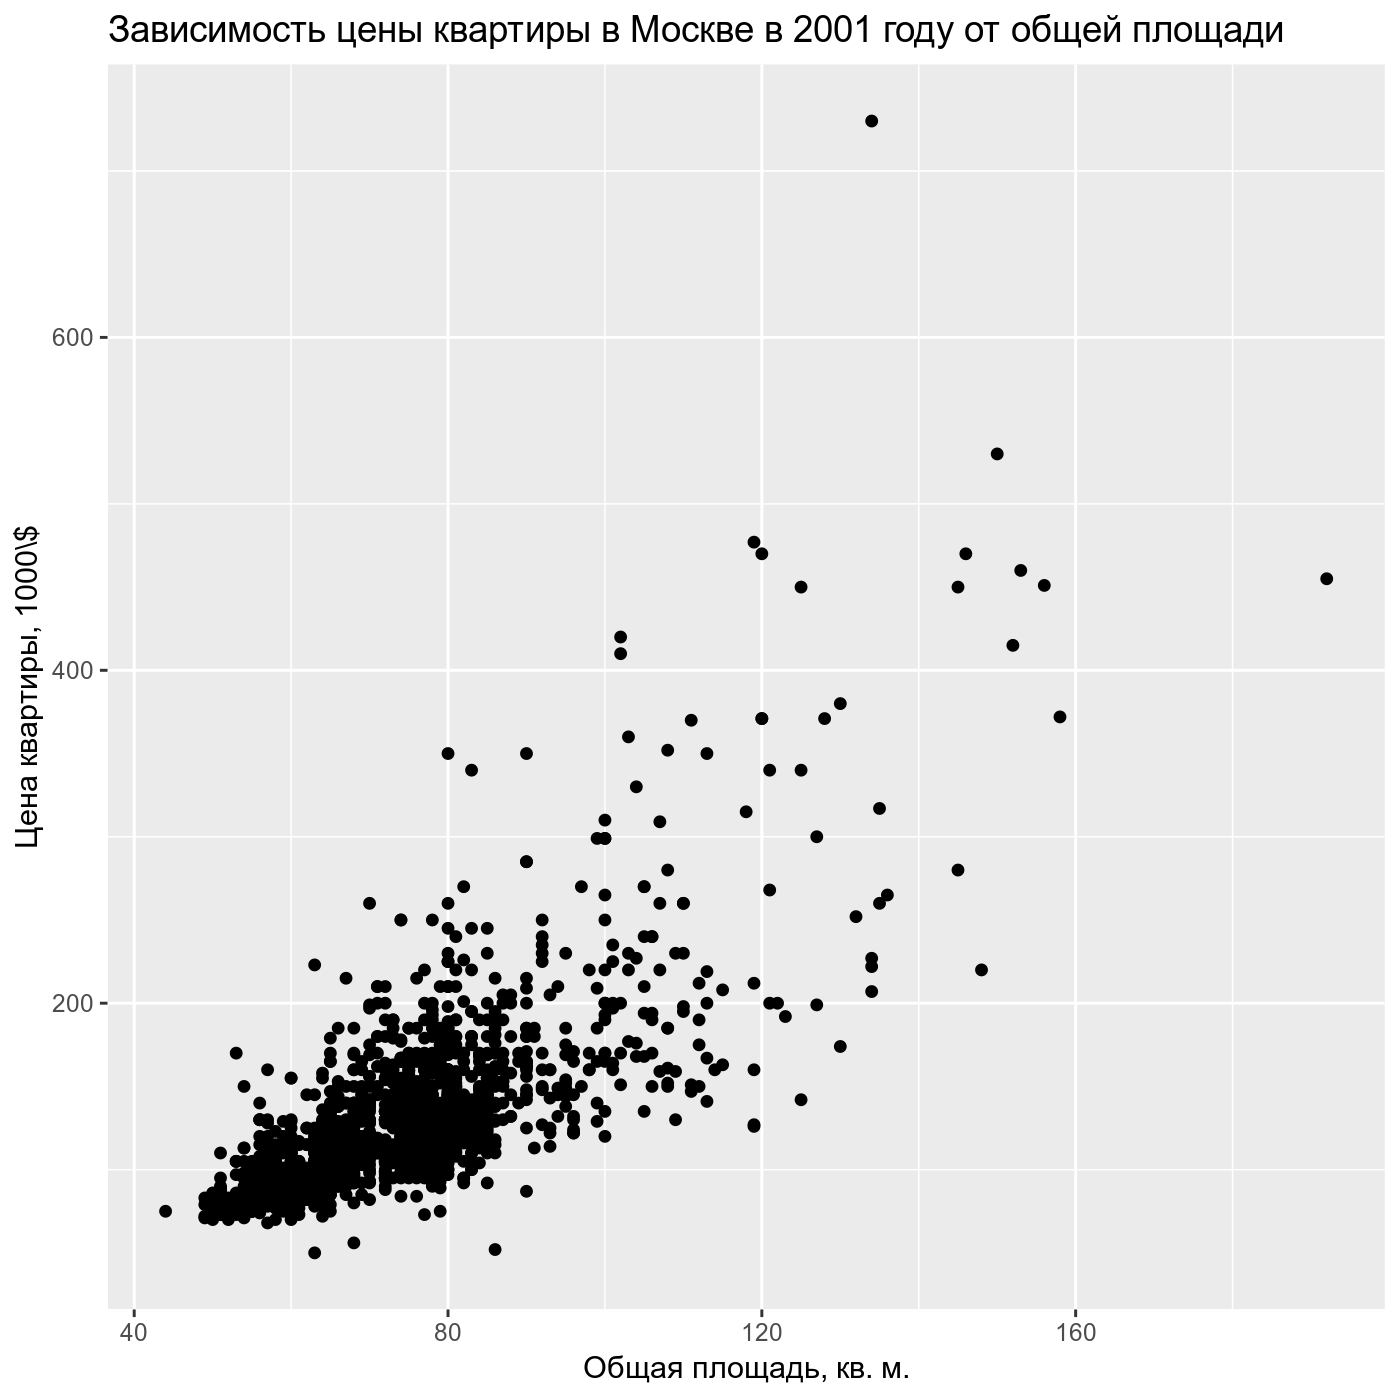
\includegraphics[scale=0.65]{R_plots/flats_scatter.png}
\end{center}
\end{minipage}


Какие подходы к оцениванию зависимости имеет смысл посоветовать исходя из данного графика?



\begin{sol}
По графику видно, что с увеличением общей площади увеличивается разброс цены. Поэтому разумно, например, рассмотреть следующие подходы:
\begin{enumerate}
\item Перейти к логарифмам, т.е. оценивать модель $\ln price_i=\beta_1+\beta_2 \ln totsp_i +\varepsilon_i$.
\item Оценивать квантильную регрессию. В ней угловые коэффициенты линейной зависимости будут отличаться для разных квантилей переменной $price$.
\item Обычную модель линейной регрессии с гетероскедастичностью вида $\Var(\varepsilon_i)=\sigma^2 totsp_i^2$.
\end{enumerate}
\end{sol}
\end{problem}




\begin{problem}
По наблюдениям $x=(1,2,3)'$, $y=(2,-1,3)'$ оценивается модель $y=\b_1+\b_2 x+\e$. Ошибки $\e$ гетероскедастичны и известно, что $\Var(\e_i)=\sigma^2 \cdot x_i^2$.
\begin{enumerate}
\item Найдите оценки $\hb_{ols}$ с помощью МНК и их ковариационную матрицу.
\item Найдите оценки $\hb_{gls}$ с помощью обобщенного МНК и их ковариационную матрицу.
\end{enumerate}


\begin{sol}
\end{sol}
\end{problem}





\begin{problem}
Для линейной регрессии $y_i = \beta_1 + \beta_2 x_i + \beta_3 z_i + \e_i$ была
выполнена сортировка наблюдений по возрастанию переменной $x$. Исходная модель оценивалась по разным частям выборки:

\begin{tabular}{c|cccc}
\toprule
Выборка & $\hb_1$ & $\hb_2$ & $\hb_3$ & $RSS$ \\
\midrule
$i=1,\ldots, 30$ & $1.21$ & $1.89$ & $2.74$ & $48.69$ \\
$i=1,\ldots, 11$ & $1.39$ & $2.27$ & $2.36$ & $10.28$ \\
$i=12,\ldots, 19$ & $0.75$ & $2.23$ & $3.19$ & $5.31$ \\
$i=20,\ldots, 30$ & $1.56$ & $1.06$ & $2.29$ & $14.51$ \\
\bottomrule
\end{tabular}

Известно, что ошибки в модели являются независимыми нормальными случайными величинами с нулевым математическим ожиданием. Протестируйте
ошибки на гетероскедастичность на уровне значимости 5\%.



\begin{sol}
Протестируем гетероскедастичность ошибок при помощи теста Голдфельда-
Квандта. $H_0: \Var(\e_i)=\sigma^2$, $H_a: \Var(\e_i)=f(x_i)$

\begin{enumerate}
\item Тестовая статистика $GQ=\frac{RSS_3/(n_3-k)}{RSS_1/(n_1-k)}$, где $n_1=11$ — число наблюдений в первой подгруппе, $n_3=11$ — число наблюдений в
последней подгруппе, $k=3$ — число факторов в модели, считая единичный столбец.
\item Распределение тестовой статистики при верной $H_0$: $GQ\sim F_{n_3-k,n_1-k}$
\item Наблюдаемое значение $GQ_{obs}=1.41$
\item Область, в которой $H_0$ не отвергается: $GQ\in [0;3.44]$
\item Статистический вывод: поскольку $GQ_{obs} \in [0;3.44]$, то на основании имеющихся наблюдений на уровне значимости 5\% основная гипотеза $H_0$ не может быть отвергнута. Таким образом, тест Голдфельда-Квандта не выявил гетероскедастичность.
\end{enumerate}
\end{sol}
\end{problem}



\begin{problem}
Для линейной регрессии $y_i = \beta_1 + \beta_2 x_i + \beta_3 z_i + \e_i$ была
выполнена сортировка наблюдений по возрастанию переменной $x$. Исходная модель оценивалась по разным частям выборки:

\begin{tabular}{c|cccc}
\toprule
Выборка & $\hb_1$ & $\hb_2$ & $\hb_3$ & $RSS$ \\
\midrule
$i=1,\ldots, 50$ & $1.16$ & $1.99$ & $2.97$ & $174.69$ \\
$i=1,\ldots, 21$ & $0.76$ & $2.25$ & $3.18$ & $20.41$ \\
$i=22,\ldots, 29$ & $0.85$ & $1.81$ & $3.32$ & $3.95$ \\
$i=30,\ldots, 50$ & $1.72$ & $1.41$ & $2.49$ & $130.74$ \\
\bottomrule
\end{tabular}

Известно, что ошибки в модели являются независимыми нормальными случайными величинами с нулевым математическим ожиданием. Протестируйте
ошибки на гетероскедастичность на уровне значимости 1\%.


\begin{sol}
Протестируем гетероскедастичность ошибок при помощи теста Голдфельда-
Квандта. $H_0: \Var(\e_i)=\sigma^2$, $H_a: \Var(\e_i)=f(x_i)$

\begin{enumerate}
\item Тестовая статистика $GQ=\frac{RSS_3/(n_3-k)}{RSS_1/(n_1-k)}$, где $n_1=21$ — число наблюдений в первой подгруппе, $n_3=21$ — число наблюдений в
последней подгруппе, $k=3$ — число факторов в модели, считая единичный столбец.
\item Распределение тестовой статистики при верной $H_0$: $GQ\sim F_{n_3-k,n_1-k}$
\item Наблюдаемое значение $GQ_{obs}=6.49$
\item Область, в которой $H_0$ не отвергается: $GQ\in [0;3.12]$
\item Статистический вывод: поскольку $GQ_{obs} \notin [0;3.12]$, то на основании имеющихся наблюдений на уровне значимости 1\% основная гипотеза $H_0$ отвергается. Таким образом, тест Голдфельда-Квандта выявил гетероскедастичность.
\end{enumerate}
\end{sol}
\end{problem}



\begin{problem}
Для линейной регрессии $y_i = \beta_1 + \beta_2 x_i + \beta_3 z_i + \e_i$ была
выполнена сортировка наблюдений по возрастанию переменной $x$. Исходная модель оценивалась по разным частям выборки:

\begin{tabular}{c|cccc}
\toprule
Выборка & $\hb_1$ & $\hb_2$ & $\hb_3$ & $RSS$ \\
\midrule
$i=1,\ldots, 30$ & $0.96$ & $2.25$ & $3.44$ & $52.70$ \\
$i=1,\ldots, 11$ & $1.07$ & $2.46$ & $2.40$ & $5.55$ \\
$i=12,\ldots, 19$ & $1.32$ & $1.01$ & $2.88$ & $11.69$ \\
$i=20,\ldots, 30$ & $1.04$ & $2.56$ & $4.12$ & $16.00$ \\
\bottomrule
\end{tabular}

Известно, что ошибки в модели являются независимыми нормальными случайными величинами с нулевым математическим ожиданием. Протестируйте
ошибки на гетероскедастичность на уровне значимости 5\%.


\begin{sol}
Протестируем гетероскедастичность ошибок при помощи теста Голдфельда-
Квандта. $H_0: \Var(\e_i)=\sigma^2$, $H_a: \Var(\e_i)=f(x_i)$

\begin{enumerate}
\item Тестовая статистика $GQ=\frac{RSS_3/(n_3-k)}{RSS_1/(n_1-k)}$, где $n_1=11$ — число наблюдений в первой подгруппе, $n_3=11$ — число наблюдений в
последней подгруппе, $k=3$ — число факторов в модели, считая единичный столбец.
\item Распределение тестовой статистики при верной $H_0$: $GQ\sim F_{n_3-k,n_1-k}$
\item Наблюдаемое значение $GQ_{obs}=2.88$
\item Область, в которой $H_0$ не отвергается: $GQ\in [0;3.44]$
\item Статистический вывод: поскольку $GQ_{obs} \in [0;3.44]$, то на основании имеющихся наблюдений на уровне значимости 5\% основная гипотеза $H_0$ не может быть отвергнута. Таким образом, тест Голдфельда-Квандта не выявил гетероскедастичность.
\end{enumerate}
\end{sol}
\end{problem}



\begin{problem}
Для линейной регрессии $y_i = \beta_1 + \beta_2 x_i + \beta_3 z_i + \e_i$ была выполнена сортировка наблюдений по возрастанию переменной $x$. Исходная модель оценивалась по разным частям выборки:

\begin{tabular}{c|cccc}
\toprule
Выборка & $\hb_1$ & $\hb_2$ & $\hb_3$ & $RSS$ \\
\midrule
$i=1,\ldots, 50$ & $0.93$ & $2.02$ & $3.38$ & $145.85$ \\
$i=1,\ldots, 21$ & $1.12$ & $2.01$ & $3.32$ & $19.88$ \\
$i=22,\ldots, 29$ & $0.29$ & $2.07$ & $2.24$ & $1.94$ \\
$i=30,\ldots, 50$ & $0.87$ & $1.84$ & $3.66$ & $117.46$ \\
\bottomrule
\end{tabular}

Известно, что ошибки в модели являются независимыми нормальными случайными величинами с нулевым математическим ожиданием. Протестируйте
ошибки на гетероскедастичность на уровне значимости 5\%.

\begin{sol}
Протестируем гетероскедастичность ошибок при помощи теста Голдфельда-
Квандта. $H_0: \Var(\e_i)=\sigma^2$, $H_a: \Var(\e_i)=f(x_i)$

\begin{enumerate}
\item Тестовая статистика $GQ=\frac{RSS_3/(n_3-k)}{RSS_1/(n_1-k)}$, где $n_1=21$ — число наблюдений в первой подгруппе, $n_3=21$ — число наблюдений в
последней подгруппе, $k=3$ — число факторов в модели, считая единичный столбец.
\item Распределение тестовой статистики при верной $H_0$: $GQ\sim F_{n_3-k,n_1-k}$
\item Наблюдаемое значение $GQ_{obs}=5.91$
\item Область, в которой $H_0$ не отвергается: $GQ\in [0;2.21]$
\item Статистический вывод: поскольку $GQ_{obs} \notin [0;2.21]$, то на основании имеющихся наблюдений на уровне значимости 5\% основная гипотеза $H_0$ отвергается. Таким образом, тест Голдфельда-Квандта выявил гетероскедастичность.
\end{enumerate}
\end{sol}
\end{problem}



\begin{problem}
Рассмотрим линейную регрессию $y_i = \beta_1 + \beta_2 x_i + \beta_3 z_i + \e_i$ по 50 наблюдениям. При оценивании с помощью МНК были получены результаты: $\hb_1=1.21$, $\hb_2=1.11$, $\hb_3=3.15$, $R^2=0.72$.

Оценена также вспомогательная регрессия: $\he^2_i=\delta_1+\delta_2 x_i +\delta_3 z_i+\delta_4 x_i^2+\delta_5 z_i^2+\delta_6 x_i z_i + u_i$. Результаты оценивания следующие: $\hat{\delta}_1=1.50$, $\hat{\delta}_2=-2.18$,  $\hat{\delta}_3=0.23$,  $\hat{\delta}_4=1.87$,  $\hat{\delta}_5=-0.56$,  $\hat{\delta}_6=-0.09$,  $R^2_{aux}=0.36$


Известно, что ошибки в модели являются независимыми нормальными случайными величинами с нулевым математическим ожиданием. Протестируйте
ошибки на гетероскедастичность на уровне значимости 5\%.


\begin{sol}
Протестируем гетероскедастичность ошибок при помощи теста Уайта. $H_0: \Var(\e_i)=\sigma^2$, $H_a: \Var(\e_i)=\delta_1+\delta_2 x_i +\delta_3 z_i+\delta_4 x_i^2+\delta_5 z_i^2+\delta_6 x_i z_i$.
\begin{enumerate}
\item Тестовая статистика $W=n\cdot R^2_{aux}$, где $n$ — число наблюдений, $R^2_{aux}$ — коэффициент детерминации для вспомогательной регрессии.
\item Распределение тестовой статистики при верной $H_0$: $W\sim \chi^2_{k_{aux}-1}$, где $k_{aux}=6$ — число регрессоров во вспомогательной регрессии, считая константу.
\item Наблюдаемое значение тестовой статистики: $W_{obs}=18$
\item Область, в которой $H_0$ не отвергается: $W\in [0;W_{crit}]=[0;11.07]$
\item Статистический вывод: поскольку $W_{obs} \notin [0;11.07]$, то на основании имеющихся наблюдений на уровне значимости 5\% основная гипотеза $H_0$ отвергается. Таким образом, тест Уайта выявил гетероскедастичность.
\end{enumerate}
\end{sol}
\end{problem}




\begin{problem}
Объясните, с какой целью используются стандартные ошибки в форме Уайта. Приведите развернутый ответ. Верно ли, что стандартные ошибки в форме Уайта позволяют
\begin{enumerate}
\item устранить гетероскедастичность?
\item корректно тестировать гипотезы относительно коэффициентов регрессии в условиях гетероскедастичности?
\end{enumerate}


\begin{sol}
\end{sol}
\end{problem}



\begin{problem}
Объясните, с какой целью используются стандартные ошибки в форме Невье–Веста. Приведите развернутый ответ. Верно ли, что стандартные ошибки в форме Невье–Веста позволяют
\begin{enumerate}
\item устранить гетероскедастичность?
\item корректно тестировать гипотезы относительно коэффициентов регрессии в условиях гетероскедастичности?
\end{enumerate}


\begin{sol}
\end{sol}
\end{problem}



\begin{problem}
Рассматривается модель $y_t=\beta_1+\e_t$, где ошибки $\e_t$  — независимые
случайные величины с $\E(\e_t)=0$ и $\Var(\e_t)=t$. Найдите наиболее эффективную
оценку неизвестного параметра $\beta_1$ в классе линейных по $y$ и несмещённых оценок.

\begin{sol}
\end{sol}
\end{problem}


\begin{problem}
Рассматривается модель $y_t=\beta_1+\e_t$, где ошибки $\e_t$  — независимые
случайные величины с $\E(\e_t)=0$ и $\Var(\e_t)=t^2$. Найдите наиболее эффективную
оценку неизвестного параметра $\beta_1$ в классе линейных по $y$ и несмещённых оценок.

\begin{sol}
\end{sol}
\end{problem}



\begin{problem}
Рассматривается модель $y_t=\beta_1 x_t+\e_t$, где ошибки $\e_t$  — независимые
случайные величины с $\E(\e_t)=0$ и $\Var(\e_t)=t$. Найдите наиболее эффективную
оценку неизвестного параметра $\beta_1$ в классе линейных по $y$ и несмещённых оценок.

\begin{sol}
\end{sol}
\end{problem}



\begin{problem}
Рассматривается модель $y_t=\beta_1 x_t +\e_t$, где ошибки $\e_t$  — независимые
случайные величины с $\E(\e_t)=0$ и $\Var(\e_t)=t^2$. Найдите наиболее эффективную
оценку неизвестного параметра $\beta_1$ в классе линейных по $y$ и несмещённых оценок.

\begin{sol}
\end{sol}
\end{problem}



\begin{problem}
Докажите, что в условиях гетероскедастичности МНК-оценки остаются несмещёнными.


\begin{sol}
\[
\E(\hb|X) = \E((X'X)^{-1}X'y|X)=(X'X)^{-1}X'\E(X\beta + u|X)=\beta + \E(u|X)=\beta
\]
\end{sol}
\end{problem}



\begin{problem}
Оценка коэффициентов обобщенного МНК имеет вид $\hb_{GLS}=(X'V^{-1}X)^{-1}X'V^{-1}y$, где $V=\Var(\e)$. Совпадает ли оценка $\hb_{GLS}$ с оценкой обычным МНК в условиях гомоскедастичности?


\begin{sol}
\end{sol}
\end{problem}



\begin{problem}
Модель $y_i=\beta_1 + \beta_2 x_i +\e_i$ оценивается по трём наблюдениям, $y=(9,3,6)$, $x=(1,2,4)$. Имеется гетероскедастичность вида $\Var(\e_i)=\sigma^2 x_i^2$, ошибки $\e_i$ нормально распределены.
\begin{enumerate}
\item Оцените $\beta$ с помощью МНК, проигнорировав гетероскедастичность. Постройте 95\% доверительный интервал для каждого коэффициента, проигнорировав гетероскедастичность.
\item Оцените $\beta$ с помощью обобщенного МНК, учитывая гетероскедастичность. Постройте 95\% доверительный интервал для каждого коэффициента, учитывая гетероскедастичности.
\end{enumerate}


\begin{sol}
\end{sol}
\end{problem}



\begin{problem}
Рассмотрим модель $y_i=\beta_1+\beta_2 x_i+\e_i$, где ошибки $\e_i$ некоррелированы, $\E(\e_i)=0$, $\Var(\e_i)=\sigma^2_i$. Предлагается два способа оценить коэффициенты модели:
\begin{enumerate}
\item[WLS.] Взвешенный метод наименьших квадратов. Поделим каждое уравнение $y_i=\beta_1+\beta_2 x_i+\e_i$ на $\sigma_i$. Затем обычным методом наименьших квадратов в преобразованной модели $y_i/\sigma_i=\beta_1\cdot 1/\sigma_i+\beta_2 x_i/\sigma_i+\e_i/\sigma_i$ найдем оценки $\hb_{WLS}$.
\item[GLS.] Обобщенный метод наименьших квадратов. Оценки $\hb_{GLS}$ находим по формуле $\hb_{GLS}=(X'V^{-1}X)^{-1}X'V^{-1}y$, где
\[
V=\Var(\e)=\begin{pmatrix}
\sigma^2_1 & 0 & 0 \\
0 & \ddots & 0 \\
0 & 0 & \sigma^2_n
\end{pmatrix}
\]
\end{enumerate}
\begin{enumerate}
\item Докажите, что в матричном виде преобразование взвешенного МНК записывается как $V^{-1/2}y=V^{-1/2}X\beta+V^{-1/2}\e$.
\item Верно ли, что $\hb_{WLS}=\hb_{GLS}$?
\item Найдите $\E(\hb_{WLS})$, $\Var(\hb_{WLGS})$
\item В явном виде выпишите $\hb_{2,WLS}$.
\end{enumerate}


\begin{sol}
\end{sol}
\end{problem}




\begin{problem}
Рассмотрим модель регрессии $y_i=\beta_1+\beta_2 x_i + \beta_3 z_i+\e_i$, в которой
ошибки $\e_i$ независимы и имеют нормальное распределение $N(0,\sigma^2)$. Для $n = 200$ наблюдений найдите
\begin{enumerate}
\item вероятность того, что статистика Уайта окажется больше 10;
\item ожидаемое значение статистики Уайта;
\item дисперсию статистики Уайта.
\end{enumerate}


\begin{sol}
$0.0752$, $5$, $10$
\end{sol}
\end{problem}


\begin{problem}
Найдите число коэффициентов во вспомогательной регрессии, необходимой для выполнения теста Уайта, если число коэффициентов в исходной регрессии равно $k$, включая свободный член.


\begin{sol}
$k(k+1)/2$
\end{sol}
\end{problem}


\begin{problem}
По 35 наблюдениям сотрудники НИИ оценили уравнение регрессии $y_i = \beta_1 + \beta_2 x_i + \e_i$ и рассчитали остатки $\e_i$. После того они приступили к диагностике возможных недостатков модели, обнаружили гетероскедастичность и решили её побороть.
\begin{enumerate}
\item Самый младший научный сотрудник выдвинул предположение, что стандартное отклонение случайной составляющей может быть выражено так: $\sigma_{\e, i} = a x_i$, где $a$ — неизвестный коэффициент. Каким образом нужно преобразовать исходное уравнение регрессии, чтобы избавиться от гетероскедастичности?
\item Профессор решил перепроверить результаты и оценил регрессию:
\[
\hat{e}_i^2 = -0.3 + 0.08 x_i - 0.01 x_i^2, R^2 = 0.15.
\]
Свидетельствует ли полученный профессором результат о наличии гетероскедастичности?
\end{enumerate}


\begin{sol}
\end{sol}
\end{problem}



\begin{problem}
Пусть $y_t = \beta x_t + \e$ где $\E(\e_t) = 0$ и известно, что оценки для параметров $\tilde{\beta} = \left( \sum_{t=1}^n y_t \right)/\left( \sum_{t=1}^n x_t \right)$ являются наилучшими (в смысле минимума дисперсии) среди линейных несмещённых оценок параметра $\beta$. 
Чему равна в этом случае матрица ковариаций вектора $\e$ с точностью до пропорциональности?



\begin{sol}
Известно, что оценки параметров, получаемые по обобщённому методу наименьших квадратов, являются наилучшими, поэтому:
\[
\Var(\e) = const \cdot 
\begin{pmatrix}
x_1     & 0      & \cdots & 0 \\
0       & x_2    & \cdots & 0 \\
\vdots  & \vdots & \ddots & \vdots \\
0       & 0      & \cdots & x_n \\
\end{pmatrix}
\]
\end{sol}
\end{problem}


\begin{problem}
Для регрессии $y = X\beta + \e$ с $\E(\e) = 0$, $\Var(\e) = \Sigma \neq \sigma^2 I$, оцененной с помощью обобщённого метода наименьших квадратов, найдите ковариационную матрицу $\Cov(\hb_{GLS}, \e)$



\begin{sol}
\begin{multline*}
\Cov(\hb_{GLS}, \e) = \Cov \left( (X' \Sigma^{-1} X)^{-1} X' \Sigma^{-1} y, \e \right) = \\
= \Cov \left( (X' \Sigma^{-1} X)^{-1} X' \Sigma^{-1} \e, \e \right) = \\
= (X' \Sigma^{-1} X)^{-1} X' \Sigma^{-1} \Cov(\e, \e) =\\
= (X' \Sigma^{-1} X)^{-1} X' \Sigma^{-1} \Sigma = (X' \Sigma^{-1} X)^{-1} X'
\end{multline*}
\end{sol}
\end{problem}



\begin{problem}
Найдите наиболее эффективную оценку коэффициента $\beta_1$ для модели $y_i = \beta + \e$, $\E(\e_i) = 0$, $\E(\e_i\e_j) = 0$, $\Var(\e_i) = \sigma_{\e}^2 / x_i$, $x_i > 0$ в классе линейных несмещённых оценок


\begin{sol}
Для нахождения эффективной оценки воспользуемся взвешенным методом наименьших квадратов. Разделим каждое из уравнений $y_i = \beta + \e$ на корень из дисперсии $\e_i$ с тем, чтобы ошибки в полученных уравнениях имели равные дисперсии (в этом случае можно будет сослаться на т. Гаусса-Маркова). Итак, после деления i-го уравнения на величину $\sqrt{x_i}/\sigma_{\e}$, мы получаем:
\[
\begin{pmatrix}
y_1 \sqrt{x_1}/\sigma_{\e} \\
y_2 \sqrt{x_2}/\sigma_{\e} \\
\ldots \\
y_n \sqrt{x_n}/\sigma_{\e} \\
\end{pmatrix} = \beta \begin{pmatrix}
\sqrt{x_1}/\sigma_{\e} \\
\sqrt{x_2}/\sigma_{\e} \\
\ldots \\
\sqrt{x_n}/\sigma_{\e} \\
\end{pmatrix} + \begin{pmatrix}
\e_1 \sqrt{x_1}/\sigma_{\e} \\
\e_2 \sqrt{x_2}/\sigma_{\e} \\
\ldots \\
\e_n \sqrt{x_n}/\sigma_{\e} \\
\end{pmatrix}
\]
Поскольку условия т. Гаусса-Маркова для последней модели выполнены, то МНК-оценка для последней модели будет наиболее эффективной. Поэтому
\[
\hb = \frac{\sum_{i=1}^n (y_i \sqrt{x_i}/\sigma_{\e})(\sqrt{x_i}/\sigma_{\e})}{\sum_{i=1}^n (\sqrt{x_i}/\sigma_{\e})^2} = \frac{\sum_{i=1}^n y_i x_i}{\sum_{i=1}^n x_i}
\]
\end{sol}
\end{problem}



\begin{problem}
Исследователь оценил регрессионную модель $y_i = \beta_1 + \beta_2 x_i + \beta_3 z_i + \beta_4 w_i + \e_i$ и провёл диагностику различных проблемных явлений. 
Результаты его стараний приведены ниже:

\begin{minted}[mathescape, numbersep=5pt, frame=lines, framesep=2mm]{r}
set.seed(777)
n <- 200
x <- rnorm(n)
z <- rnorm(n)
w <- rnorm(n)
eps <- abs(x)*rnorm(n)
y <- 2 + 3 * x - 3 * z + 1 * w + eps
model <- lm(y ~ x + z + w)
resid <- resid(model)
plot1 <- qplot(x, abs(resid),
  xlab = "Переменная $x$",
  ylab = "Модуль остатка")
plot2 <- qplot(head(resid, -1),
       tail(resid, -1),
       xlab = "Остаток $\\hat\\varepsilon_{t-1}$",
       ylab = "Остаток $\\hat\\varepsilon_{t}$")
grid.arrange(plot1, plot2, ncol = 2)
\end{minted}



\begin{minipage}{0.6\textwidth}
\begin{center}
\begin{tikzpicture}[scale = 0.025]
% Created by tikzDevice version 0.12 on 2019-05-28 10:03:32
% !TEX encoding = UTF-8 Unicode
\definecolor{fillColor}{RGB}{255,255,255}
\path[use as bounding box,fill=fillColor,fill opacity=0.00] (0,0) rectangle (505.89,505.89);
\begin{scope}
\path[clip] (  0.00,  0.00) rectangle (252.94,505.89);
\definecolor{drawColor}{RGB}{255,255,255}
\definecolor{fillColor}{RGB}{255,255,255}

\path[draw=drawColor,line width= 0.6pt,line join=round,line cap=round,fill=fillColor] (  0.00,  0.00) rectangle (252.94,505.89);
\end{scope}
\begin{scope}
\path[clip] ( 27.42, 31.51) rectangle (247.45,500.39);
\definecolor{fillColor}{gray}{0.92}

\path[fill=fillColor] ( 27.42, 31.51) rectangle (247.44,500.39);
\definecolor{drawColor}{RGB}{255,255,255}

\path[draw=drawColor,line width= 0.3pt,line join=round] ( 27.42,103.75) --
	(247.45,103.75);

\path[draw=drawColor,line width= 0.3pt,line join=round] ( 27.42,206.09) --
	(247.45,206.09);

\path[draw=drawColor,line width= 0.3pt,line join=round] ( 27.42,308.43) --
	(247.45,308.43);

\path[draw=drawColor,line width= 0.3pt,line join=round] ( 27.42,410.76) --
	(247.45,410.76);

\path[draw=drawColor,line width= 0.3pt,line join=round] ( 57.78, 31.51) --
	( 57.78,500.39);

\path[draw=drawColor,line width= 0.3pt,line join=round] ( 92.20, 31.51) --
	( 92.20,500.39);

\path[draw=drawColor,line width= 0.3pt,line join=round] (126.62, 31.51) --
	(126.62,500.39);

\path[draw=drawColor,line width= 0.3pt,line join=round] (161.04, 31.51) --
	(161.04,500.39);

\path[draw=drawColor,line width= 0.3pt,line join=round] (195.46, 31.51) --
	(195.46,500.39);

\path[draw=drawColor,line width= 0.3pt,line join=round] (229.89, 31.51) --
	(229.89,500.39);

\path[draw=drawColor,line width= 0.6pt,line join=round] ( 27.42, 52.58) --
	(247.45, 52.58);

\path[draw=drawColor,line width= 0.6pt,line join=round] ( 27.42,154.92) --
	(247.45,154.92);

\path[draw=drawColor,line width= 0.6pt,line join=round] ( 27.42,257.26) --
	(247.45,257.26);

\path[draw=drawColor,line width= 0.6pt,line join=round] ( 27.42,359.59) --
	(247.45,359.59);

\path[draw=drawColor,line width= 0.6pt,line join=round] ( 27.42,461.93) --
	(247.45,461.93);

\path[draw=drawColor,line width= 0.6pt,line join=round] ( 40.57, 31.51) --
	( 40.57,500.39);

\path[draw=drawColor,line width= 0.6pt,line join=round] ( 74.99, 31.51) --
	( 74.99,500.39);

\path[draw=drawColor,line width= 0.6pt,line join=round] (109.41, 31.51) --
	(109.41,500.39);

\path[draw=drawColor,line width= 0.6pt,line join=round] (143.83, 31.51) --
	(143.83,500.39);

\path[draw=drawColor,line width= 0.6pt,line join=round] (178.25, 31.51) --
	(178.25,500.39);

\path[draw=drawColor,line width= 0.6pt,line join=round] (212.67, 31.51) --
	(212.67,500.39);

\path[draw=drawColor,line width= 0.6pt,line join=round] (247.10, 31.51) --
	(247.10,500.39);
\definecolor{drawColor}{RGB}{0,0,0}
\definecolor{fillColor}{RGB}{0,0,0}

\path[draw=drawColor,line width= 0.4pt,line join=round,line cap=round,fill=fillColor] (160.69, 60.71) circle (  1.96);

\path[draw=drawColor,line width= 0.4pt,line join=round,line cap=round,fill=fillColor] (130.11,109.24) circle (  1.96);

\path[draw=drawColor,line width= 0.4pt,line join=round,line cap=round,fill=fillColor] (161.42, 60.70) circle (  1.96);

\path[draw=drawColor,line width= 0.4pt,line join=round,line cap=round,fill=fillColor] (130.10,119.65) circle (  1.96);

\path[draw=drawColor,line width= 0.4pt,line join=round,line cap=round,fill=fillColor] (200.24,147.99) circle (  1.96);

\path[draw=drawColor,line width= 0.4pt,line join=round,line cap=round,fill=fillColor] (165.22,141.37) circle (  1.96);

\path[draw=drawColor,line width= 0.4pt,line join=round,line cap=round,fill=fillColor] (150.81, 58.19) circle (  1.96);

\path[draw=drawColor,line width= 0.4pt,line join=round,line cap=round,fill=fillColor] (182.00,185.07) circle (  1.96);

\path[draw=drawColor,line width= 0.4pt,line join=round,line cap=round,fill=fillColor] (136.73, 56.54) circle (  1.96);

\path[draw=drawColor,line width= 0.4pt,line join=round,line cap=round,fill=fillColor] (130.79, 94.03) circle (  1.96);

\path[draw=drawColor,line width= 0.4pt,line join=round,line cap=round,fill=fillColor] (133.36, 82.60) circle (  1.96);

\path[draw=drawColor,line width= 0.4pt,line join=round,line cap=round,fill=fillColor] (145.70, 55.68) circle (  1.96);

\path[draw=drawColor,line width= 0.4pt,line join=round,line cap=round,fill=fillColor] ( 79.09,168.59) circle (  1.96);

\path[draw=drawColor,line width= 0.4pt,line join=round,line cap=round,fill=fillColor] (142.67, 69.09) circle (  1.96);

\path[draw=drawColor,line width= 0.4pt,line join=round,line cap=round,fill=fillColor] (223.40,250.56) circle (  1.96);

\path[draw=drawColor,line width= 0.4pt,line join=round,line cap=round,fill=fillColor] (177.30,243.62) circle (  1.96);

\path[draw=drawColor,line width= 0.4pt,line join=round,line cap=round,fill=fillColor] (177.04, 99.59) circle (  1.96);

\path[draw=drawColor,line width= 0.4pt,line join=round,line cap=round,fill=fillColor] (125.10, 54.63) circle (  1.96);

\path[draw=drawColor,line width= 0.4pt,line join=round,line cap=round,fill=fillColor] (166.94,111.90) circle (  1.96);

\path[draw=drawColor,line width= 0.4pt,line join=round,line cap=round,fill=fillColor] (161.07,103.75) circle (  1.96);

\path[draw=drawColor,line width= 0.4pt,line join=round,line cap=round,fill=fillColor] ( 73.94, 86.64) circle (  1.96);

\path[draw=drawColor,line width= 0.4pt,line join=round,line cap=round,fill=fillColor] (151.67, 75.92) circle (  1.96);

\path[draw=drawColor,line width= 0.4pt,line join=round,line cap=round,fill=fillColor] (116.88,142.42) circle (  1.96);

\path[draw=drawColor,line width= 0.4pt,line join=round,line cap=round,fill=fillColor] (187.67, 84.49) circle (  1.96);

\path[draw=drawColor,line width= 0.4pt,line join=round,line cap=round,fill=fillColor] (193.32,117.41) circle (  1.96);

\path[draw=drawColor,line width= 0.4pt,line join=round,line cap=round,fill=fillColor] (158.53, 87.19) circle (  1.96);

\path[draw=drawColor,line width= 0.4pt,line join=round,line cap=round,fill=fillColor] ( 83.79, 52.86) circle (  1.96);

\path[draw=drawColor,line width= 0.4pt,line join=round,line cap=round,fill=fillColor] (142.96, 61.82) circle (  1.96);

\path[draw=drawColor,line width= 0.4pt,line join=round,line cap=round,fill=fillColor] ( 92.60,161.29) circle (  1.96);

\path[draw=drawColor,line width= 0.4pt,line join=round,line cap=round,fill=fillColor] (125.19, 65.73) circle (  1.96);

\path[draw=drawColor,line width= 0.4pt,line join=round,line cap=round,fill=fillColor] (166.60,110.89) circle (  1.96);

\path[draw=drawColor,line width= 0.4pt,line join=round,line cap=round,fill=fillColor] (173.38,186.17) circle (  1.96);

\path[draw=drawColor,line width= 0.4pt,line join=round,line cap=round,fill=fillColor] (186.92,128.77) circle (  1.96);

\path[draw=drawColor,line width= 0.4pt,line join=round,line cap=round,fill=fillColor] (102.02,206.02) circle (  1.96);

\path[draw=drawColor,line width= 0.4pt,line join=round,line cap=round,fill=fillColor] (196.26,134.82) circle (  1.96);

\path[draw=drawColor,line width= 0.4pt,line join=round,line cap=round,fill=fillColor] (101.29, 61.59) circle (  1.96);

\path[draw=drawColor,line width= 0.4pt,line join=round,line cap=round,fill=fillColor] (201.17,196.63) circle (  1.96);

\path[draw=drawColor,line width= 0.4pt,line join=round,line cap=round,fill=fillColor] (126.50,101.36) circle (  1.96);

\path[draw=drawColor,line width= 0.4pt,line join=round,line cap=round,fill=fillColor] (123.92, 90.06) circle (  1.96);

\path[draw=drawColor,line width= 0.4pt,line join=round,line cap=round,fill=fillColor] (153.19, 55.03) circle (  1.96);

\path[draw=drawColor,line width= 0.4pt,line join=round,line cap=round,fill=fillColor] (133.46, 84.85) circle (  1.96);

\path[draw=drawColor,line width= 0.4pt,line join=round,line cap=round,fill=fillColor] (129.52, 53.02) circle (  1.96);

\path[draw=drawColor,line width= 0.4pt,line join=round,line cap=round,fill=fillColor] (118.66, 94.05) circle (  1.96);

\path[draw=drawColor,line width= 0.4pt,line join=round,line cap=round,fill=fillColor] (115.11, 67.33) circle (  1.96);

\path[draw=drawColor,line width= 0.4pt,line join=round,line cap=round,fill=fillColor] (165.44,101.18) circle (  1.96);

\path[draw=drawColor,line width= 0.4pt,line join=round,line cap=round,fill=fillColor] (171.29,160.81) circle (  1.96);

\path[draw=drawColor,line width= 0.4pt,line join=round,line cap=round,fill=fillColor] (118.71, 73.32) circle (  1.96);

\path[draw=drawColor,line width= 0.4pt,line join=round,line cap=round,fill=fillColor] (115.07, 64.11) circle (  1.96);

\path[draw=drawColor,line width= 0.4pt,line join=round,line cap=round,fill=fillColor] (132.02, 96.82) circle (  1.96);

\path[draw=drawColor,line width= 0.4pt,line join=round,line cap=round,fill=fillColor] (194.91,121.52) circle (  1.96);

\path[draw=drawColor,line width= 0.4pt,line join=round,line cap=round,fill=fillColor] (196.59,161.63) circle (  1.96);

\path[draw=drawColor,line width= 0.4pt,line join=round,line cap=round,fill=fillColor] (102.18, 81.73) circle (  1.96);

\path[draw=drawColor,line width= 0.4pt,line join=round,line cap=round,fill=fillColor] (224.04,260.39) circle (  1.96);

\path[draw=drawColor,line width= 0.4pt,line join=round,line cap=round,fill=fillColor] (141.43, 68.52) circle (  1.96);

\path[draw=drawColor,line width= 0.4pt,line join=round,line cap=round,fill=fillColor] (152.48, 95.90) circle (  1.96);

\path[draw=drawColor,line width= 0.4pt,line join=round,line cap=round,fill=fillColor] (155.54, 75.17) circle (  1.96);

\path[draw=drawColor,line width= 0.4pt,line join=round,line cap=round,fill=fillColor] (125.66, 73.02) circle (  1.96);

\path[draw=drawColor,line width= 0.4pt,line join=round,line cap=round,fill=fillColor] (155.28, 88.96) circle (  1.96);

\path[draw=drawColor,line width= 0.4pt,line join=round,line cap=round,fill=fillColor] ( 59.96, 70.55) circle (  1.96);

\path[draw=drawColor,line width= 0.4pt,line join=round,line cap=round,fill=fillColor] (171.54, 60.95) circle (  1.96);

\path[draw=drawColor,line width= 0.4pt,line join=round,line cap=round,fill=fillColor] (131.65,129.78) circle (  1.96);

\path[draw=drawColor,line width= 0.4pt,line join=round,line cap=round,fill=fillColor] (149.88, 87.87) circle (  1.96);

\path[draw=drawColor,line width= 0.4pt,line join=round,line cap=round,fill=fillColor] (141.07, 54.32) circle (  1.96);

\path[draw=drawColor,line width= 0.4pt,line join=round,line cap=round,fill=fillColor] ( 88.60,110.66) circle (  1.96);

\path[draw=drawColor,line width= 0.4pt,line join=round,line cap=round,fill=fillColor] (187.54,273.96) circle (  1.96);

\path[draw=drawColor,line width= 0.4pt,line join=round,line cap=round,fill=fillColor] (137.51,106.90) circle (  1.96);

\path[draw=drawColor,line width= 0.4pt,line join=round,line cap=round,fill=fillColor] (123.84, 59.70) circle (  1.96);

\path[draw=drawColor,line width= 0.4pt,line join=round,line cap=round,fill=fillColor] (146.61, 68.35) circle (  1.96);

\path[draw=drawColor,line width= 0.4pt,line join=round,line cap=round,fill=fillColor] (126.89, 70.92) circle (  1.96);

\path[draw=drawColor,line width= 0.4pt,line join=round,line cap=round,fill=fillColor] (138.14, 82.49) circle (  1.96);

\path[draw=drawColor,line width= 0.4pt,line join=round,line cap=round,fill=fillColor] (176.86,115.40) circle (  1.96);

\path[draw=drawColor,line width= 0.4pt,line join=round,line cap=round,fill=fillColor] (118.02, 74.55) circle (  1.96);

\path[draw=drawColor,line width= 0.4pt,line join=round,line cap=round,fill=fillColor] ( 96.32,158.23) circle (  1.96);

\path[draw=drawColor,line width= 0.4pt,line join=round,line cap=round,fill=fillColor] (160.23, 70.12) circle (  1.96);

\path[draw=drawColor,line width= 0.4pt,line join=round,line cap=round,fill=fillColor] (102.69,218.63) circle (  1.96);

\path[draw=drawColor,line width= 0.4pt,line join=round,line cap=round,fill=fillColor] (164.78,121.24) circle (  1.96);

\path[draw=drawColor,line width= 0.4pt,line join=round,line cap=round,fill=fillColor] (128.48, 72.37) circle (  1.96);

\path[draw=drawColor,line width= 0.4pt,line join=round,line cap=round,fill=fillColor] (149.02, 67.85) circle (  1.96);

\path[draw=drawColor,line width= 0.4pt,line join=round,line cap=round,fill=fillColor] (110.42, 77.44) circle (  1.96);

\path[draw=drawColor,line width= 0.4pt,line join=round,line cap=round,fill=fillColor] (160.58,115.87) circle (  1.96);

\path[draw=drawColor,line width= 0.4pt,line join=round,line cap=round,fill=fillColor] (172.40,138.98) circle (  1.96);

\path[draw=drawColor,line width= 0.4pt,line join=round,line cap=round,fill=fillColor] (144.09, 62.90) circle (  1.96);

\path[draw=drawColor,line width= 0.4pt,line join=round,line cap=round,fill=fillColor] (179.60,147.75) circle (  1.96);

\path[draw=drawColor,line width= 0.4pt,line join=round,line cap=round,fill=fillColor] (142.91, 61.26) circle (  1.96);

\path[draw=drawColor,line width= 0.4pt,line join=round,line cap=round,fill=fillColor] (139.12, 62.75) circle (  1.96);

\path[draw=drawColor,line width= 0.4pt,line join=round,line cap=round,fill=fillColor] (145.87, 59.46) circle (  1.96);

\path[draw=drawColor,line width= 0.4pt,line join=round,line cap=round,fill=fillColor] (113.94, 95.27) circle (  1.96);

\path[draw=drawColor,line width= 0.4pt,line join=round,line cap=round,fill=fillColor] (111.78,133.20) circle (  1.96);

\path[draw=drawColor,line width= 0.4pt,line join=round,line cap=round,fill=fillColor] (173.38, 86.34) circle (  1.96);

\path[draw=drawColor,line width= 0.4pt,line join=round,line cap=round,fill=fillColor] ( 95.00,152.62) circle (  1.96);

\path[draw=drawColor,line width= 0.4pt,line join=round,line cap=round,fill=fillColor] ( 84.02,192.84) circle (  1.96);

\path[draw=drawColor,line width= 0.4pt,line join=round,line cap=round,fill=fillColor] (124.23, 99.47) circle (  1.96);

\path[draw=drawColor,line width= 0.4pt,line join=round,line cap=round,fill=fillColor] (170.27,156.71) circle (  1.96);

\path[draw=drawColor,line width= 0.4pt,line join=round,line cap=round,fill=fillColor] (112.88,200.44) circle (  1.96);

\path[draw=drawColor,line width= 0.4pt,line join=round,line cap=round,fill=fillColor] (187.15,152.96) circle (  1.96);

\path[draw=drawColor,line width= 0.4pt,line join=round,line cap=round,fill=fillColor] (115.89,192.76) circle (  1.96);

\path[draw=drawColor,line width= 0.4pt,line join=round,line cap=round,fill=fillColor] (128.64, 61.52) circle (  1.96);

\path[draw=drawColor,line width= 0.4pt,line join=round,line cap=round,fill=fillColor] (170.43,128.53) circle (  1.96);

\path[draw=drawColor,line width= 0.4pt,line join=round,line cap=round,fill=fillColor] (128.38, 55.28) circle (  1.96);

\path[draw=drawColor,line width= 0.4pt,line join=round,line cap=round,fill=fillColor] (157.29, 55.07) circle (  1.96);

\path[draw=drawColor,line width= 0.4pt,line join=round,line cap=round,fill=fillColor] (173.39,147.67) circle (  1.96);

\path[draw=drawColor,line width= 0.4pt,line join=round,line cap=round,fill=fillColor] (149.67, 67.19) circle (  1.96);

\path[draw=drawColor,line width= 0.4pt,line join=round,line cap=round,fill=fillColor] (160.10, 91.01) circle (  1.96);

\path[draw=drawColor,line width= 0.4pt,line join=round,line cap=round,fill=fillColor] (105.54,249.92) circle (  1.96);

\path[draw=drawColor,line width= 0.4pt,line join=round,line cap=round,fill=fillColor] (187.98,274.32) circle (  1.96);

\path[draw=drawColor,line width= 0.4pt,line join=round,line cap=round,fill=fillColor] (181.06,255.70) circle (  1.96);

\path[draw=drawColor,line width= 0.4pt,line join=round,line cap=round,fill=fillColor] (151.36, 55.90) circle (  1.96);

\path[draw=drawColor,line width= 0.4pt,line join=round,line cap=round,fill=fillColor] (159.47,133.84) circle (  1.96);

\path[draw=drawColor,line width= 0.4pt,line join=round,line cap=round,fill=fillColor] ( 96.81,140.03) circle (  1.96);

\path[draw=drawColor,line width= 0.4pt,line join=round,line cap=round,fill=fillColor] (139.02, 60.07) circle (  1.96);

\path[draw=drawColor,line width= 0.4pt,line join=round,line cap=round,fill=fillColor] (186.97,258.34) circle (  1.96);

\path[draw=drawColor,line width= 0.4pt,line join=round,line cap=round,fill=fillColor] (163.06,170.87) circle (  1.96);

\path[draw=drawColor,line width= 0.4pt,line join=round,line cap=round,fill=fillColor] (152.42,113.51) circle (  1.96);

\path[draw=drawColor,line width= 0.4pt,line join=round,line cap=round,fill=fillColor] (128.90, 88.93) circle (  1.96);

\path[draw=drawColor,line width= 0.4pt,line join=round,line cap=round,fill=fillColor] (154.39, 68.12) circle (  1.96);

\path[draw=drawColor,line width= 0.4pt,line join=round,line cap=round,fill=fillColor] (104.50,125.84) circle (  1.96);

\path[draw=drawColor,line width= 0.4pt,line join=round,line cap=round,fill=fillColor] (127.63, 84.05) circle (  1.96);

\path[draw=drawColor,line width= 0.4pt,line join=round,line cap=round,fill=fillColor] (140.78, 53.29) circle (  1.96);

\path[draw=drawColor,line width= 0.4pt,line join=round,line cap=round,fill=fillColor] (159.79,105.37) circle (  1.96);

\path[draw=drawColor,line width= 0.4pt,line join=round,line cap=round,fill=fillColor] (144.23, 57.48) circle (  1.96);

\path[draw=drawColor,line width= 0.4pt,line join=round,line cap=round,fill=fillColor] (155.36, 89.79) circle (  1.96);

\path[draw=drawColor,line width= 0.4pt,line join=round,line cap=round,fill=fillColor] (109.39,116.99) circle (  1.96);

\path[draw=drawColor,line width= 0.4pt,line join=round,line cap=round,fill=fillColor] (104.29,164.13) circle (  1.96);

\path[draw=drawColor,line width= 0.4pt,line join=round,line cap=round,fill=fillColor] (138.50, 65.18) circle (  1.96);

\path[draw=drawColor,line width= 0.4pt,line join=round,line cap=round,fill=fillColor] (119.03, 60.25) circle (  1.96);

\path[draw=drawColor,line width= 0.4pt,line join=round,line cap=round,fill=fillColor] (167.09, 65.43) circle (  1.96);

\path[draw=drawColor,line width= 0.4pt,line join=round,line cap=round,fill=fillColor] (161.39, 83.64) circle (  1.96);

\path[draw=drawColor,line width= 0.4pt,line join=round,line cap=round,fill=fillColor] (172.44,173.07) circle (  1.96);

\path[draw=drawColor,line width= 0.4pt,line join=round,line cap=round,fill=fillColor] (194.51,173.94) circle (  1.96);

\path[draw=drawColor,line width= 0.4pt,line join=round,line cap=round,fill=fillColor] (197.60,227.40) circle (  1.96);

\path[draw=drawColor,line width= 0.4pt,line join=round,line cap=round,fill=fillColor] (125.56, 67.98) circle (  1.96);

\path[draw=drawColor,line width= 0.4pt,line join=round,line cap=round,fill=fillColor] (111.59, 65.01) circle (  1.96);

\path[draw=drawColor,line width= 0.4pt,line join=round,line cap=round,fill=fillColor] (174.63,108.62) circle (  1.96);

\path[draw=drawColor,line width= 0.4pt,line join=round,line cap=round,fill=fillColor] (166.40,110.03) circle (  1.96);

\path[draw=drawColor,line width= 0.4pt,line join=round,line cap=round,fill=fillColor] (138.63, 64.43) circle (  1.96);

\path[draw=drawColor,line width= 0.4pt,line join=round,line cap=round,fill=fillColor] (101.28,206.15) circle (  1.96);

\path[draw=drawColor,line width= 0.4pt,line join=round,line cap=round,fill=fillColor] (210.85,215.22) circle (  1.96);

\path[draw=drawColor,line width= 0.4pt,line join=round,line cap=round,fill=fillColor] (200.73,264.25) circle (  1.96);

\path[draw=drawColor,line width= 0.4pt,line join=round,line cap=round,fill=fillColor] (236.67,434.32) circle (  1.96);

\path[draw=drawColor,line width= 0.4pt,line join=round,line cap=round,fill=fillColor] (100.87,263.09) circle (  1.96);

\path[draw=drawColor,line width= 0.4pt,line join=round,line cap=round,fill=fillColor] (123.35, 88.22) circle (  1.96);

\path[draw=drawColor,line width= 0.4pt,line join=round,line cap=round,fill=fillColor] (158.09,101.85) circle (  1.96);

\path[draw=drawColor,line width= 0.4pt,line join=round,line cap=round,fill=fillColor] (151.36, 82.74) circle (  1.96);

\path[draw=drawColor,line width= 0.4pt,line join=round,line cap=round,fill=fillColor] (188.60,197.75) circle (  1.96);

\path[draw=drawColor,line width= 0.4pt,line join=round,line cap=round,fill=fillColor] (130.76, 98.25) circle (  1.96);

\path[draw=drawColor,line width= 0.4pt,line join=round,line cap=round,fill=fillColor] (184.42, 70.44) circle (  1.96);

\path[draw=drawColor,line width= 0.4pt,line join=round,line cap=round,fill=fillColor] (108.09, 86.19) circle (  1.96);

\path[draw=drawColor,line width= 0.4pt,line join=round,line cap=round,fill=fillColor] (138.87, 61.86) circle (  1.96);

\path[draw=drawColor,line width= 0.4pt,line join=round,line cap=round,fill=fillColor] (118.92,103.49) circle (  1.96);

\path[draw=drawColor,line width= 0.4pt,line join=round,line cap=round,fill=fillColor] (161.64, 85.30) circle (  1.96);

\path[draw=drawColor,line width= 0.4pt,line join=round,line cap=round,fill=fillColor] (153.86, 61.17) circle (  1.96);

\path[draw=drawColor,line width= 0.4pt,line join=round,line cap=round,fill=fillColor] (163.25, 71.80) circle (  1.96);

\path[draw=drawColor,line width= 0.4pt,line join=round,line cap=round,fill=fillColor] (148.26, 95.54) circle (  1.96);

\path[draw=drawColor,line width= 0.4pt,line join=round,line cap=round,fill=fillColor] (180.40,274.74) circle (  1.96);

\path[draw=drawColor,line width= 0.4pt,line join=round,line cap=round,fill=fillColor] (102.66, 60.35) circle (  1.96);

\path[draw=drawColor,line width= 0.4pt,line join=round,line cap=round,fill=fillColor] ( 98.82,104.22) circle (  1.96);

\path[draw=drawColor,line width= 0.4pt,line join=round,line cap=round,fill=fillColor] (124.66, 88.90) circle (  1.96);

\path[draw=drawColor,line width= 0.4pt,line join=round,line cap=round,fill=fillColor] (143.66, 57.62) circle (  1.96);

\path[draw=drawColor,line width= 0.4pt,line join=round,line cap=round,fill=fillColor] (122.19, 53.52) circle (  1.96);

\path[draw=drawColor,line width= 0.4pt,line join=round,line cap=round,fill=fillColor] (190.76,226.87) circle (  1.96);

\path[draw=drawColor,line width= 0.4pt,line join=round,line cap=round,fill=fillColor] (146.05, 61.47) circle (  1.96);

\path[draw=drawColor,line width= 0.4pt,line join=round,line cap=round,fill=fillColor] (159.32, 54.70) circle (  1.96);

\path[draw=drawColor,line width= 0.4pt,line join=round,line cap=round,fill=fillColor] ( 92.58, 61.71) circle (  1.96);

\path[draw=drawColor,line width= 0.4pt,line join=round,line cap=round,fill=fillColor] ( 79.00,273.70) circle (  1.96);

\path[draw=drawColor,line width= 0.4pt,line join=round,line cap=round,fill=fillColor] (177.53, 87.49) circle (  1.96);

\path[draw=drawColor,line width= 0.4pt,line join=round,line cap=round,fill=fillColor] ( 97.25, 94.13) circle (  1.96);

\path[draw=drawColor,line width= 0.4pt,line join=round,line cap=round,fill=fillColor] (111.61,130.74) circle (  1.96);

\path[draw=drawColor,line width= 0.4pt,line join=round,line cap=round,fill=fillColor] ( 65.66,299.91) circle (  1.96);

\path[draw=drawColor,line width= 0.4pt,line join=round,line cap=round,fill=fillColor] (116.46,106.38) circle (  1.96);

\path[draw=drawColor,line width= 0.4pt,line join=round,line cap=round,fill=fillColor] (136.26,102.97) circle (  1.96);

\path[draw=drawColor,line width= 0.4pt,line join=round,line cap=round,fill=fillColor] (226.58,356.41) circle (  1.96);

\path[draw=drawColor,line width= 0.4pt,line join=round,line cap=round,fill=fillColor] (148.58, 59.64) circle (  1.96);

\path[draw=drawColor,line width= 0.4pt,line join=round,line cap=round,fill=fillColor] (135.09,121.63) circle (  1.96);

\path[draw=drawColor,line width= 0.4pt,line join=round,line cap=round,fill=fillColor] (133.89, 84.93) circle (  1.96);

\path[draw=drawColor,line width= 0.4pt,line join=round,line cap=round,fill=fillColor] ( 81.93,116.60) circle (  1.96);

\path[draw=drawColor,line width= 0.4pt,line join=round,line cap=round,fill=fillColor] (196.83,287.05) circle (  1.96);

\path[draw=drawColor,line width= 0.4pt,line join=round,line cap=round,fill=fillColor] (136.44, 52.82) circle (  1.96);

\path[draw=drawColor,line width= 0.4pt,line join=round,line cap=round,fill=fillColor] (237.44, 59.67) circle (  1.96);

\path[draw=drawColor,line width= 0.4pt,line join=round,line cap=round,fill=fillColor] (107.36,118.48) circle (  1.96);

\path[draw=drawColor,line width= 0.4pt,line join=round,line cap=round,fill=fillColor] (141.96, 54.47) circle (  1.96);

\path[draw=drawColor,line width= 0.4pt,line join=round,line cap=round,fill=fillColor] (119.92,215.40) circle (  1.96);

\path[draw=drawColor,line width= 0.4pt,line join=round,line cap=round,fill=fillColor] (138.88, 52.94) circle (  1.96);

\path[draw=drawColor,line width= 0.4pt,line join=round,line cap=round,fill=fillColor] (169.04, 88.35) circle (  1.96);

\path[draw=drawColor,line width= 0.4pt,line join=round,line cap=round,fill=fillColor] (132.48, 87.39) circle (  1.96);

\path[draw=drawColor,line width= 0.4pt,line join=round,line cap=round,fill=fillColor] ( 99.38,132.04) circle (  1.96);

\path[draw=drawColor,line width= 0.4pt,line join=round,line cap=round,fill=fillColor] (160.50,101.54) circle (  1.96);

\path[draw=drawColor,line width= 0.4pt,line join=round,line cap=round,fill=fillColor] (149.88, 64.43) circle (  1.96);

\path[draw=drawColor,line width= 0.4pt,line join=round,line cap=round,fill=fillColor] (161.05, 85.95) circle (  1.96);

\path[draw=drawColor,line width= 0.4pt,line join=round,line cap=round,fill=fillColor] (175.77,359.53) circle (  1.96);

\path[draw=drawColor,line width= 0.4pt,line join=round,line cap=round,fill=fillColor] ( 98.15, 59.33) circle (  1.96);

\path[draw=drawColor,line width= 0.4pt,line join=round,line cap=round,fill=fillColor] (159.82, 73.58) circle (  1.96);

\path[draw=drawColor,line width= 0.4pt,line join=round,line cap=round,fill=fillColor] (166.37,164.14) circle (  1.96);

\path[draw=drawColor,line width= 0.4pt,line join=round,line cap=round,fill=fillColor] ( 37.42,479.08) circle (  1.96);

\path[draw=drawColor,line width= 0.4pt,line join=round,line cap=round,fill=fillColor] (166.76, 90.03) circle (  1.96);

\path[draw=drawColor,line width= 0.4pt,line join=round,line cap=round,fill=fillColor] (171.07,131.55) circle (  1.96);

\path[draw=drawColor,line width= 0.4pt,line join=round,line cap=round,fill=fillColor] (106.58,105.11) circle (  1.96);

\path[draw=drawColor,line width= 0.4pt,line join=round,line cap=round,fill=fillColor] (138.01, 74.99) circle (  1.96);

\path[draw=drawColor,line width= 0.4pt,line join=round,line cap=round,fill=fillColor] (130.86,144.92) circle (  1.96);

\path[draw=drawColor,line width= 0.4pt,line join=round,line cap=round,fill=fillColor] (117.21,163.36) circle (  1.96);

\path[draw=drawColor,line width= 0.4pt,line join=round,line cap=round,fill=fillColor] (126.46, 76.07) circle (  1.96);
\end{scope}
\begin{scope}
\path[clip] (  0.00,  0.00) rectangle (505.89,505.89);
\definecolor{drawColor}{gray}{0.30}

\node[text=drawColor,anchor=base east,inner sep=0pt, outer sep=0pt, scale=  0.73] at ( 22.47, 49.55) {0};

\node[text=drawColor,anchor=base east,inner sep=0pt, outer sep=0pt, scale=  0.73] at ( 22.47,151.89) {1};

\node[text=drawColor,anchor=base east,inner sep=0pt, outer sep=0pt, scale=  0.73] at ( 22.47,254.23) {2};

\node[text=drawColor,anchor=base east,inner sep=0pt, outer sep=0pt, scale=  0.73] at ( 22.47,356.56) {3};

\node[text=drawColor,anchor=base east,inner sep=0pt, outer sep=0pt, scale=  0.73] at ( 22.47,458.90) {4};
\end{scope}
\begin{scope}
\path[clip] (  0.00,  0.00) rectangle (505.89,505.89);
\definecolor{drawColor}{gray}{0.20}

\path[draw=drawColor,line width= 0.6pt,line join=round] ( 24.67, 52.58) --
	( 27.42, 52.58);

\path[draw=drawColor,line width= 0.6pt,line join=round] ( 24.67,154.92) --
	( 27.42,154.92);

\path[draw=drawColor,line width= 0.6pt,line join=round] ( 24.67,257.26) --
	( 27.42,257.26);

\path[draw=drawColor,line width= 0.6pt,line join=round] ( 24.67,359.59) --
	( 27.42,359.59);

\path[draw=drawColor,line width= 0.6pt,line join=round] ( 24.67,461.93) --
	( 27.42,461.93);
\end{scope}
\begin{scope}
\path[clip] (  0.00,  0.00) rectangle (505.89,505.89);
\definecolor{drawColor}{gray}{0.20}

\path[draw=drawColor,line width= 0.6pt,line join=round] ( 40.57, 28.76) --
	( 40.57, 31.51);

\path[draw=drawColor,line width= 0.6pt,line join=round] ( 74.99, 28.76) --
	( 74.99, 31.51);

\path[draw=drawColor,line width= 0.6pt,line join=round] (109.41, 28.76) --
	(109.41, 31.51);

\path[draw=drawColor,line width= 0.6pt,line join=round] (143.83, 28.76) --
	(143.83, 31.51);

\path[draw=drawColor,line width= 0.6pt,line join=round] (178.25, 28.76) --
	(178.25, 31.51);

\path[draw=drawColor,line width= 0.6pt,line join=round] (212.67, 28.76) --
	(212.67, 31.51);

\path[draw=drawColor,line width= 0.6pt,line join=round] (247.10, 28.76) --
	(247.10, 31.51);
\end{scope}
\begin{scope}
\path[clip] (  0.00,  0.00) rectangle (505.89,505.89);
\definecolor{drawColor}{gray}{0.30}

\node[text=drawColor,anchor=base,inner sep=0pt, outer sep=0pt, scale=  0.73] at ( 40.57, 20.49) {-3};

\node[text=drawColor,anchor=base,inner sep=0pt, outer sep=0pt, scale=  0.73] at ( 74.99, 20.49) {-2};

\node[text=drawColor,anchor=base,inner sep=0pt, outer sep=0pt, scale=  0.73] at (109.41, 20.49) {-1};

\node[text=drawColor,anchor=base,inner sep=0pt, outer sep=0pt, scale=  0.73] at (143.83, 20.49) {0};

\node[text=drawColor,anchor=base,inner sep=0pt, outer sep=0pt, scale=  0.73] at (178.25, 20.49) {1};

\node[text=drawColor,anchor=base,inner sep=0pt, outer sep=0pt, scale=  0.73] at (212.67, 20.49) {2};

\node[text=drawColor,anchor=base,inner sep=0pt, outer sep=0pt, scale=  0.73] at (247.10, 20.49) {3};
\end{scope}
\begin{scope}
\path[clip] (  0.00,  0.00) rectangle (505.89,505.89);
\definecolor{drawColor}{RGB}{0,0,0}

\node[text=drawColor,anchor=base,inner sep=0pt, outer sep=0pt, scale=  0.92] at (137.43,  7.83) {Переменная $x$};
\end{scope}
\begin{scope}
\path[clip] (  0.00,  0.00) rectangle (505.89,505.89);
\definecolor{drawColor}{RGB}{0,0,0}

\node[text=drawColor,rotate= 90.00,anchor=base,inner sep=0pt, outer sep=0pt, scale=  0.92] at ( 13.08,265.95) {Модуль остатков};
\end{scope}
\begin{scope}
\path[clip] (252.94,  0.00) rectangle (505.89,505.89);
\definecolor{drawColor}{RGB}{255,255,255}
\definecolor{fillColor}{RGB}{255,255,255}

\path[draw=drawColor,line width= 0.6pt,line join=round,line cap=round,fill=fillColor] (252.94,  0.00) rectangle (505.89,505.89);
\end{scope}
\begin{scope}
\path[clip] (283.24, 31.51) rectangle (500.39,500.39);
\definecolor{fillColor}{gray}{0.92}

\path[fill=fillColor] (283.24, 31.51) rectangle (500.39,500.39);
\definecolor{drawColor}{RGB}{255,255,255}

\path[draw=drawColor,line width= 0.3pt,line join=round] (283.24,115.83) --
	(500.39,115.83);

\path[draw=drawColor,line width= 0.3pt,line join=round] (283.24,223.78) --
	(500.39,223.78);

\path[draw=drawColor,line width= 0.3pt,line join=round] (283.24,331.72) --
	(500.39,331.72);

\path[draw=drawColor,line width= 0.3pt,line join=round] (283.24,439.67) --
	(500.39,439.67);

\path[draw=drawColor,line width= 0.3pt,line join=round] (322.29, 31.51) --
	(322.29,500.39);

\path[draw=drawColor,line width= 0.3pt,line join=round] (372.28, 31.51) --
	(372.28,500.39);

\path[draw=drawColor,line width= 0.3pt,line join=round] (422.28, 31.51) --
	(422.28,500.39);

\path[draw=drawColor,line width= 0.3pt,line join=round] (472.27, 31.51) --
	(472.27,500.39);

\path[draw=drawColor,line width= 0.6pt,line join=round] (283.24, 61.86) --
	(500.39, 61.86);

\path[draw=drawColor,line width= 0.6pt,line join=round] (283.24,169.81) --
	(500.39,169.81);

\path[draw=drawColor,line width= 0.6pt,line join=round] (283.24,277.75) --
	(500.39,277.75);

\path[draw=drawColor,line width= 0.6pt,line join=round] (283.24,385.70) --
	(500.39,385.70);

\path[draw=drawColor,line width= 0.6pt,line join=round] (283.24,493.64) --
	(500.39,493.64);

\path[draw=drawColor,line width= 0.6pt,line join=round] (297.29, 31.51) --
	(297.29,500.39);

\path[draw=drawColor,line width= 0.6pt,line join=round] (347.29, 31.51) --
	(347.29,500.39);

\path[draw=drawColor,line width= 0.6pt,line join=round] (397.28, 31.51) --
	(397.28,500.39);

\path[draw=drawColor,line width= 0.6pt,line join=round] (447.27, 31.51) --
	(447.27,500.39);

\path[draw=drawColor,line width= 0.6pt,line join=round] (497.26, 31.51) --
	(497.26,500.39);
\definecolor{drawColor}{RGB}{0,0,0}
\definecolor{fillColor}{RGB}{0,0,0}

\path[draw=drawColor,line width= 0.4pt,line join=round,line cap=round,fill=fillColor] (395.29,307.63) circle (  1.96);

\path[draw=drawColor,line width= 0.4pt,line join=round,line cap=round,fill=fillColor] (411.12,282.03) circle (  1.96);

\path[draw=drawColor,line width= 0.4pt,line join=round,line cap=round,fill=fillColor] (399.26,242.38) circle (  1.96);

\path[draw=drawColor,line width= 0.4pt,line join=round,line cap=round,fill=fillColor] (380.90,227.43) circle (  1.96);

\path[draw=drawColor,line width= 0.4pt,line join=round,line cap=round,fill=fillColor] (373.98,230.92) circle (  1.96);

\path[draw=drawColor,line width= 0.4pt,line join=round,line cap=round,fill=fillColor] (375.59,274.79) circle (  1.96);

\path[draw=drawColor,line width= 0.4pt,line join=round,line cap=round,fill=fillColor] (395.91,207.88) circle (  1.96);

\path[draw=drawColor,line width= 0.4pt,line join=round,line cap=round,fill=fillColor] (364.92,279.84) circle (  1.96);

\path[draw=drawColor,line width= 0.4pt,line join=round,line cap=round,fill=fillColor] (398.25,255.89) circle (  1.96);

\path[draw=drawColor,line width= 0.4pt,line join=round,line cap=round,fill=fillColor] (387.16,293.58) circle (  1.96);

\path[draw=drawColor,line width= 0.4pt,line join=round,line cap=round,fill=fillColor] (404.61,279.39) circle (  1.96);

\path[draw=drawColor,line width= 0.4pt,line join=round,line cap=round,fill=fillColor] (398.04,338.94) circle (  1.96);

\path[draw=drawColor,line width= 0.4pt,line join=round,line cap=round,fill=fillColor] (425.62,286.46) circle (  1.96);

\path[draw=drawColor,line width= 0.4pt,line join=round,line cap=round,fill=fillColor] (401.31,173.34) circle (  1.96);

\path[draw=drawColor,line width= 0.4pt,line join=round,line cap=round,fill=fillColor] (348.92,378.50) circle (  1.96);

\path[draw=drawColor,line width= 0.4pt,line join=round,line cap=round,fill=fillColor] (443.94,302.54) circle (  1.96);

\path[draw=drawColor,line width= 0.4pt,line join=round,line cap=round,fill=fillColor] (408.76,278.83) circle (  1.96);

\path[draw=drawColor,line width= 0.4pt,line join=round,line cap=round,fill=fillColor] (397.78,309.04) circle (  1.96);

\path[draw=drawColor,line width= 0.4pt,line join=round,line cap=round,fill=fillColor] (411.77,250.76) circle (  1.96);

\path[draw=drawColor,line width= 0.4pt,line join=round,line cap=round,fill=fillColor] (384.78,259.79) circle (  1.96);

\path[draw=drawColor,line width= 0.4pt,line join=round,line cap=round,fill=fillColor] (388.96,265.44) circle (  1.96);

\path[draw=drawColor,line width= 0.4pt,line join=round,line cap=round,fill=fillColor] (391.58,230.37) circle (  1.96);

\path[draw=drawColor,line width= 0.4pt,line join=round,line cap=round,fill=fillColor] (375.34,260.92) circle (  1.96);

\path[draw=drawColor,line width= 0.4pt,line join=round,line cap=round,fill=fillColor] (389.49,243.56) circle (  1.96);

\path[draw=drawColor,line width= 0.4pt,line join=round,line cap=round,fill=fillColor] (381.44,296.00) circle (  1.96);

\path[draw=drawColor,line width= 0.4pt,line join=round,line cap=round,fill=fillColor] (405.73,277.90) circle (  1.96);

\path[draw=drawColor,line width= 0.4pt,line join=round,line cap=round,fill=fillColor] (397.35,272.88) circle (  1.96);

\path[draw=drawColor,line width= 0.4pt,line join=round,line cap=round,fill=fillColor] (395.02,335.08) circle (  1.96);

\path[draw=drawColor,line width= 0.4pt,line join=round,line cap=round,fill=fillColor] (423.83,270.81) circle (  1.96);

\path[draw=drawColor,line width= 0.4pt,line join=round,line cap=round,fill=fillColor] (394.07,308.50) circle (  1.96);

\path[draw=drawColor,line width= 0.4pt,line join=round,line cap=round,fill=fillColor] (411.52,207.30) circle (  1.96);

\path[draw=drawColor,line width= 0.4pt,line join=round,line cap=round,fill=fillColor] (364.65,237.57) circle (  1.96);

\path[draw=drawColor,line width= 0.4pt,line join=round,line cap=round,fill=fillColor] (378.67,358.68) circle (  1.96);

\path[draw=drawColor,line width= 0.4pt,line join=round,line cap=round,fill=fillColor] (434.76,321.12) circle (  1.96);

\path[draw=drawColor,line width= 0.4pt,line join=round,line cap=round,fill=fillColor] (417.37,273.00) circle (  1.96);

\path[draw=drawColor,line width= 0.4pt,line join=round,line cap=round,fill=fillColor] (395.08,353.72) circle (  1.96);

\path[draw=drawColor,line width= 0.4pt,line join=round,line cap=round,fill=fillColor] (432.46,303.47) circle (  1.96);

\path[draw=drawColor,line width= 0.4pt,line join=round,line cap=round,fill=fillColor] (409.19,257.98) circle (  1.96);

\path[draw=drawColor,line width= 0.4pt,line join=round,line cap=round,fill=fillColor] (388.12,276.46) circle (  1.96);

\path[draw=drawColor,line width= 0.4pt,line join=round,line cap=round,fill=fillColor] (396.68,260.73) circle (  1.96);

\path[draw=drawColor,line width= 0.4pt,line join=round,line cap=round,fill=fillColor] (389.40,277.52) circle (  1.96);

\path[draw=drawColor,line width= 0.4pt,line join=round,line cap=round,fill=fillColor] (397.17,255.88) circle (  1.96);

\path[draw=drawColor,line width= 0.4pt,line join=round,line cap=round,fill=fillColor] (387.15,285.53) circle (  1.96);

\path[draw=drawColor,line width= 0.4pt,line join=round,line cap=round,fill=fillColor] (400.88,252.12) circle (  1.96);

\path[draw=drawColor,line width= 0.4pt,line join=round,line cap=round,fill=fillColor] (385.41,220.67) circle (  1.96);

\path[draw=drawColor,line width= 0.4pt,line join=round,line cap=round,fill=fillColor] (370.84,266.81) circle (  1.96);

\path[draw=drawColor,line width= 0.4pt,line join=round,line cap=round,fill=fillColor] (392.21,271.67) circle (  1.96);

\path[draw=drawColor,line width= 0.4pt,line join=round,line cap=round,fill=fillColor] (394.46,301.08) circle (  1.96);

\path[draw=drawColor,line width= 0.4pt,line join=round,line cap=round,fill=fillColor] (408.08,314.11) circle (  1.96);

\path[draw=drawColor,line width= 0.4pt,line join=round,line cap=round,fill=fillColor] (414.12,335.26) circle (  1.96);

\path[draw=drawColor,line width= 0.4pt,line join=round,line cap=round,fill=fillColor] (423.91,293.12) circle (  1.96);

\path[draw=drawColor,line width= 0.4pt,line join=round,line cap=round,fill=fillColor] (404.40,168.15) circle (  1.96);

\path[draw=drawColor,line width= 0.4pt,line join=round,line cap=round,fill=fillColor] (346.52,286.16) circle (  1.96);

\path[draw=drawColor,line width= 0.4pt,line join=round,line cap=round,fill=fillColor] (401.17,300.60) circle (  1.96);

\path[draw=drawColor,line width= 0.4pt,line join=round,line cap=round,fill=fillColor] (407.86,265.84) circle (  1.96);

\path[draw=drawColor,line width= 0.4pt,line join=round,line cap=round,fill=fillColor] (391.76,288.53) circle (  1.96);

\path[draw=drawColor,line width= 0.4pt,line join=round,line cap=round,fill=fillColor] (402.27,296.94) circle (  1.96);

\path[draw=drawColor,line width= 0.4pt,line join=round,line cap=round,fill=fillColor] (406.16,268.27) circle (  1.96);

\path[draw=drawColor,line width= 0.4pt,line join=round,line cap=round,fill=fillColor] (392.89,282.16) circle (  1.96);

\path[draw=drawColor,line width= 0.4pt,line join=round,line cap=round,fill=fillColor] (399.32,237.04) circle (  1.96);

\path[draw=drawColor,line width= 0.4pt,line join=round,line cap=round,fill=fillColor] (378.42,296.36) circle (  1.96);

\path[draw=drawColor,line width= 0.4pt,line join=round,line cap=round,fill=fillColor] (405.90,276.84) circle (  1.96);

\path[draw=drawColor,line width= 0.4pt,line join=round,line cap=round,fill=fillColor] (396.86,308.38) circle (  1.96);

\path[draw=drawColor,line width= 0.4pt,line join=round,line cap=round,fill=fillColor] (411.47,161.00) circle (  1.96);

\path[draw=drawColor,line width= 0.4pt,line join=round,line cap=round,fill=fillColor] (343.21,249.10) circle (  1.96);

\path[draw=drawColor,line width= 0.4pt,line join=round,line cap=round,fill=fillColor] (384.01,274.00) circle (  1.96);

\path[draw=drawColor,line width= 0.4pt,line join=round,line cap=round,fill=fillColor] (395.54,286.07) circle (  1.96);

\path[draw=drawColor,line width= 0.4pt,line join=round,line cap=round,fill=fillColor] (401.13,287.42) circle (  1.96);

\path[draw=drawColor,line width= 0.4pt,line join=round,line cap=round,fill=fillColor] (401.76,293.53) circle (  1.96);

\path[draw=drawColor,line width= 0.4pt,line join=round,line cap=round,fill=fillColor] (404.59,244.62) circle (  1.96);

\path[draw=drawColor,line width= 0.4pt,line join=round,line cap=round,fill=fillColor] (381.93,266.17) circle (  1.96);

\path[draw=drawColor,line width= 0.4pt,line join=round,line cap=round,fill=fillColor] (391.91,333.47) circle (  1.96);

\path[draw=drawColor,line width= 0.4pt,line join=round,line cap=round,fill=fillColor] (423.08,268.50) circle (  1.96);

\path[draw=drawColor,line width= 0.4pt,line join=round,line cap=round,fill=fillColor] (393.00,365.32) circle (  1.96);

\path[draw=drawColor,line width= 0.4pt,line join=round,line cap=round,fill=fillColor] (437.84,241.54) circle (  1.96);

\path[draw=drawColor,line width= 0.4pt,line join=round,line cap=round,fill=fillColor] (380.51,267.31) circle (  1.96);

\path[draw=drawColor,line width= 0.4pt,line join=round,line cap=round,fill=fillColor] (392.45,269.70) circle (  1.96);

\path[draw=drawColor,line width= 0.4pt,line join=round,line cap=round,fill=fillColor] (393.55,290.86) circle (  1.96);

\path[draw=drawColor,line width= 0.4pt,line join=round,line cap=round,fill=fillColor] (403.35,244.37) circle (  1.96);

\path[draw=drawColor,line width= 0.4pt,line join=round,line cap=round,fill=fillColor] (381.82,323.32) circle (  1.96);

\path[draw=drawColor,line width= 0.4pt,line join=round,line cap=round,fill=fillColor] (418.38,272.31) circle (  1.96);

\path[draw=drawColor,line width= 0.4pt,line join=round,line cap=round,fill=fillColor] (394.76,227.56) circle (  1.96);

\path[draw=drawColor,line width= 0.4pt,line join=round,line cap=round,fill=fillColor] (374.03,282.33) circle (  1.96);

\path[draw=drawColor,line width= 0.4pt,line join=round,line cap=round,fill=fillColor] (399.40,272.39) circle (  1.96);

\path[draw=drawColor,line width= 0.4pt,line join=round,line cap=round,fill=fillColor] (394.80,274.12) circle (  1.96);

\path[draw=drawColor,line width= 0.4pt,line join=round,line cap=round,fill=fillColor] (395.60,300.26) circle (  1.96);

\path[draw=drawColor,line width= 0.4pt,line join=round,line cap=round,fill=fillColor] (407.71,235.23) circle (  1.96);

\path[draw=drawColor,line width= 0.4pt,line join=round,line cap=round,fill=fillColor] (377.59,295.56) circle (  1.96);

\path[draw=drawColor,line width= 0.4pt,line join=round,line cap=round,fill=fillColor] (405.53,330.51) circle (  1.96);

\path[draw=drawColor,line width= 0.4pt,line join=round,line cap=round,fill=fillColor] (421.71,351.72) circle (  1.96);

\path[draw=drawColor,line width= 0.4pt,line join=round,line cap=round,fill=fillColor] (431.54,253.02) circle (  1.96);

\path[draw=drawColor,line width= 0.4pt,line join=round,line cap=round,fill=fillColor] (385.83,222.83) circle (  1.96);

\path[draw=drawColor,line width= 0.4pt,line join=round,line cap=round,fill=fillColor] (371.84,199.77) circle (  1.96);

\path[draw=drawColor,line width= 0.4pt,line join=round,line cap=round,fill=fillColor] (361.16,224.81) circle (  1.96);

\path[draw=drawColor,line width= 0.4pt,line join=round,line cap=round,fill=fillColor] (372.76,203.82) circle (  1.96);

\path[draw=drawColor,line width= 0.4pt,line join=round,line cap=round,fill=fillColor] (363.04,282.46) circle (  1.96);

\path[draw=drawColor,line width= 0.4pt,line join=round,line cap=round,fill=fillColor] (399.46,317.80) circle (  1.96);

\path[draw=drawColor,line width= 0.4pt,line join=round,line cap=round,fill=fillColor] (415.83,276.32) circle (  1.96);

\path[draw=drawColor,line width= 0.4pt,line join=round,line cap=round,fill=fillColor] (396.62,279.06) circle (  1.96);

\path[draw=drawColor,line width= 0.4pt,line join=round,line cap=round,fill=fillColor] (397.89,227.60) circle (  1.96);

\path[draw=drawColor,line width= 0.4pt,line join=round,line cap=round,fill=fillColor] (374.05,285.46) circle (  1.96);

\path[draw=drawColor,line width= 0.4pt,line join=round,line cap=round,fill=fillColor] (400.85,257.48) circle (  1.96);

\path[draw=drawColor,line width= 0.4pt,line join=round,line cap=round,fill=fillColor] (387.89,173.68) circle (  1.96);

\path[draw=drawColor,line width= 0.4pt,line join=round,line cap=round,fill=fillColor] (349.08,160.81) circle (  1.96);

\path[draw=drawColor,line width= 0.4pt,line join=round,line cap=round,fill=fillColor] (343.12,384.88) circle (  1.96);

\path[draw=drawColor,line width= 0.4pt,line join=round,line cap=round,fill=fillColor] (446.89,276.00) circle (  1.96);

\path[draw=drawColor,line width= 0.4pt,line join=round,line cap=round,fill=fillColor] (396.47,320.61) circle (  1.96);

\path[draw=drawColor,line width= 0.4pt,line join=round,line cap=round,fill=fillColor] (417.13,323.87) circle (  1.96);

\path[draw=drawColor,line width= 0.4pt,line join=round,line cap=round,fill=fillColor] (418.64,281.70) circle (  1.96);

\path[draw=drawColor,line width= 0.4pt,line join=round,line cap=round,fill=fillColor] (399.11,169.24) circle (  1.96);

\path[draw=drawColor,line width= 0.4pt,line join=round,line cap=round,fill=fillColor] (347.02,340.13) circle (  1.96);

\path[draw=drawColor,line width= 0.4pt,line join=round,line cap=round,fill=fillColor] (426.17,309.88) circle (  1.96);

\path[draw=drawColor,line width= 0.4pt,line join=round,line cap=round,fill=fillColor] (412.16,258.58) circle (  1.96);

\path[draw=drawColor,line width= 0.4pt,line join=round,line cap=round,fill=fillColor] (388.40,285.94) circle (  1.96);

\path[draw=drawColor,line width= 0.4pt,line join=round,line cap=round,fill=fillColor] (401.07,239.11) circle (  1.96);

\path[draw=drawColor,line width= 0.4pt,line join=round,line cap=round,fill=fillColor] (379.39,294.35) circle (  1.96);

\path[draw=drawColor,line width= 0.4pt,line join=round,line cap=round,fill=fillColor] (404.97,278.12) circle (  1.96);

\path[draw=drawColor,line width= 0.4pt,line join=round,line cap=round,fill=fillColor] (397.45,305.59) circle (  1.96);

\path[draw=drawColor,line width= 0.4pt,line join=round,line cap=round,fill=fillColor] (410.17,280.34) circle (  1.96);

\path[draw=drawColor,line width= 0.4pt,line join=round,line cap=round,fill=fillColor] (398.48,297.38) circle (  1.96);

\path[draw=drawColor,line width= 0.4pt,line join=round,line cap=round,fill=fillColor] (406.37,311.72) circle (  1.96);

\path[draw=drawColor,line width= 0.4pt,line join=round,line cap=round,fill=fillColor] (413.01,336.58) circle (  1.96);

\path[draw=drawColor,line width= 0.4pt,line join=round,line cap=round,fill=fillColor] (424.53,271.11) circle (  1.96);

\path[draw=drawColor,line width= 0.4pt,line join=round,line cap=round,fill=fillColor] (394.20,273.71) circle (  1.96);

\path[draw=drawColor,line width= 0.4pt,line join=round,line cap=round,fill=fillColor] (395.41,270.97) circle (  1.96);

\path[draw=drawColor,line width= 0.4pt,line join=round,line cap=round,fill=fillColor] (394.14,261.37) circle (  1.96);

\path[draw=drawColor,line width= 0.4pt,line join=round,line cap=round,fill=fillColor] (389.69,341.30) circle (  1.96);

\path[draw=drawColor,line width= 0.4pt,line join=round,line cap=round,fill=fillColor] (426.71,341.75) circle (  1.96);

\path[draw=drawColor,line width= 0.4pt,line join=round,line cap=round,fill=fillColor] (426.92,369.95) circle (  1.96);

\path[draw=drawColor,line width= 0.4pt,line join=round,line cap=round,fill=fillColor] (439.98,269.63) circle (  1.96);

\path[draw=drawColor,line width= 0.4pt,line join=round,line cap=round,fill=fillColor] (393.52,284.31) circle (  1.96);

\path[draw=drawColor,line width= 0.4pt,line join=round,line cap=round,fill=fillColor] (400.32,307.31) circle (  1.96);

\path[draw=drawColor,line width= 0.4pt,line join=round,line cap=round,fill=fillColor] (410.97,247.45) circle (  1.96);

\path[draw=drawColor,line width= 0.4pt,line join=round,line cap=round,fill=fillColor] (383.25,284.00) circle (  1.96);

\path[draw=drawColor,line width= 0.4pt,line join=round,line cap=round,fill=fillColor] (400.17,196.76) circle (  1.96);

\path[draw=drawColor,line width= 0.4pt,line join=round,line cap=round,fill=fillColor] (359.77,191.97) circle (  1.96);

\path[draw=drawColor,line width= 0.4pt,line join=round,line cap=round,fill=fillColor] (357.55,389.38) circle (  1.96);

\path[draw=drawColor,line width= 0.4pt,line join=round,line cap=round,fill=fillColor] (448.98,479.08) circle (  1.96);

\path[draw=drawColor,line width= 0.4pt,line join=round,line cap=round,fill=fillColor] (490.52,166.73) circle (  1.96);

\path[draw=drawColor,line width= 0.4pt,line join=round,line cap=round,fill=fillColor] (345.86,258.96) circle (  1.96);

\path[draw=drawColor,line width= 0.4pt,line join=round,line cap=round,fill=fillColor] (388.57,303.73) circle (  1.96);

\path[draw=drawColor,line width= 0.4pt,line join=round,line cap=round,fill=fillColor] (409.31,293.65) circle (  1.96);

\path[draw=drawColor,line width= 0.4pt,line join=round,line cap=round,fill=fillColor] (404.64,354.31) circle (  1.96);

\path[draw=drawColor,line width= 0.4pt,line join=round,line cap=round,fill=fillColor] (432.74,253.66) circle (  1.96);

\path[draw=drawColor,line width= 0.4pt,line join=round,line cap=round,fill=fillColor] (386.12,287.17) circle (  1.96);

\path[draw=drawColor,line width= 0.4pt,line join=round,line cap=round,fill=fillColor] (401.64,260.03) circle (  1.96);

\path[draw=drawColor,line width= 0.4pt,line join=round,line cap=round,fill=fillColor] (389.07,282.64) circle (  1.96);

\path[draw=drawColor,line width= 0.4pt,line join=round,line cap=round,fill=fillColor] (399.55,250.90) circle (  1.96);

\path[draw=drawColor,line width= 0.4pt,line join=round,line cap=round,fill=fillColor] (384.85,295.01) circle (  1.96);

\path[draw=drawColor,line width= 0.4pt,line join=round,line cap=round,fill=fillColor] (405.27,273.22) circle (  1.96);

\path[draw=drawColor,line width= 0.4pt,line join=round,line cap=round,fill=fillColor] (395.18,287.89) circle (  1.96);

\path[draw=drawColor,line width= 0.4pt,line join=round,line cap=round,fill=fillColor] (401.97,255.09) circle (  1.96);

\path[draw=drawColor,line width= 0.4pt,line join=round,line cap=round,fill=fillColor] (386.79,394.92) circle (  1.96);

\path[draw=drawColor,line width= 0.4pt,line join=round,line cap=round,fill=fillColor] (451.54,281.85) circle (  1.96);

\path[draw=drawColor,line width= 0.4pt,line join=round,line cap=round,fill=fillColor] (399.18,250.52) circle (  1.96);

\path[draw=drawColor,line width= 0.4pt,line join=round,line cap=round,fill=fillColor] (384.67,258.60) circle (  1.96);

\path[draw=drawColor,line width= 0.4pt,line join=round,line cap=round,fill=fillColor] (388.41,280.41) circle (  1.96);

\path[draw=drawColor,line width= 0.4pt,line join=round,line cap=round,fill=fillColor] (398.51,278.24) circle (  1.96);

\path[draw=drawColor,line width= 0.4pt,line join=round,line cap=round,fill=fillColor] (397.51,185.83) circle (  1.96);

\path[draw=drawColor,line width= 0.4pt,line join=round,line cap=round,fill=fillColor] (354.71,273.06) circle (  1.96);

\path[draw=drawColor,line width= 0.4pt,line join=round,line cap=round,fill=fillColor] (395.11,278.87) circle (  1.96);

\path[draw=drawColor,line width= 0.4pt,line join=round,line cap=round,fill=fillColor] (397.80,272.94) circle (  1.96);

\path[draw=drawColor,line width= 0.4pt,line join=round,line cap=round,fill=fillColor] (395.05,394.37) circle (  1.96);

\path[draw=drawColor,line width= 0.4pt,line join=round,line cap=round,fill=fillColor] (451.29,259.34) circle (  1.96);

\path[draw=drawColor,line width= 0.4pt,line join=round,line cap=round,fill=fillColor] (388.75,255.84) circle (  1.96);

\path[draw=drawColor,line width= 0.4pt,line join=round,line cap=round,fill=fillColor] (387.13,318.97) circle (  1.96);

\path[draw=drawColor,line width= 0.4pt,line join=round,line cap=round,fill=fillColor] (416.37,408.19) circle (  1.96);

\path[draw=drawColor,line width= 0.4pt,line join=round,line cap=round,fill=fillColor] (457.69,306.12) circle (  1.96);

\path[draw=drawColor,line width= 0.4pt,line join=round,line cap=round,fill=fillColor] (410.42,304.33) circle (  1.96);

\path[draw=drawColor,line width= 0.4pt,line join=round,line cap=round,fill=fillColor] (409.59,117.51) circle (  1.96);

\path[draw=drawColor,line width= 0.4pt,line join=round,line cap=round,fill=fillColor] (323.07,281.47) circle (  1.96);

\path[draw=drawColor,line width= 0.4pt,line join=round,line cap=round,fill=fillColor] (399.00,314.17) circle (  1.96);

\path[draw=drawColor,line width= 0.4pt,line join=round,line cap=round,fill=fillColor] (414.14,260.69) circle (  1.96);

\path[draw=drawColor,line width= 0.4pt,line join=round,line cap=round,fill=fillColor] (389.38,311.52) circle (  1.96);

\path[draw=drawColor,line width= 0.4pt,line join=round,line cap=round,fill=fillColor] (412.92,401.41) circle (  1.96);

\path[draw=drawColor,line width= 0.4pt,line join=round,line cap=round,fill=fillColor] (454.55,277.88) circle (  1.96);

\path[draw=drawColor,line width= 0.4pt,line join=round,line cap=round,fill=fillColor] (397.34,281.49) circle (  1.96);

\path[draw=drawColor,line width= 0.4pt,line join=round,line cap=round,fill=fillColor] (399.01,243.00) circle (  1.96);

\path[draw=drawColor,line width= 0.4pt,line join=round,line cap=round,fill=fillColor] (381.18,276.75) circle (  1.96);

\path[draw=drawColor,line width= 0.4pt,line join=round,line cap=round,fill=fillColor] (396.82,191.88) circle (  1.96);

\path[draw=drawColor,line width= 0.4pt,line join=round,line cap=round,fill=fillColor] (357.51,277.56) circle (  1.96);

\path[draw=drawColor,line width= 0.4pt,line join=round,line cap=round,fill=fillColor] (397.19,258.89) circle (  1.96);

\path[draw=drawColor,line width= 0.4pt,line join=round,line cap=round,fill=fillColor] (388.54,259.39) circle (  1.96);

\path[draw=drawColor,line width= 0.4pt,line join=round,line cap=round,fill=fillColor] (388.78,319.66) circle (  1.96);

\path[draw=drawColor,line width= 0.4pt,line join=round,line cap=round,fill=fillColor] (416.69,251.93) circle (  1.96);

\path[draw=drawColor,line width= 0.4pt,line join=round,line cap=round,fill=fillColor] (385.32,284.00) circle (  1.96);

\path[draw=drawColor,line width= 0.4pt,line join=round,line cap=round,fill=fillColor] (400.17,260.15) circle (  1.96);

\path[draw=drawColor,line width= 0.4pt,line join=round,line cap=round,fill=fillColor] (389.13,439.63) circle (  1.96);

\path[draw=drawColor,line width= 0.4pt,line join=round,line cap=round,fill=fillColor] (472.25,274.19) circle (  1.96);

\path[draw=drawColor,line width= 0.4pt,line join=round,line cap=round,fill=fillColor] (395.63,288.83) circle (  1.96);

\path[draw=drawColor,line width= 0.4pt,line join=round,line cap=round,fill=fillColor] (402.41,218.92) circle (  1.96);

\path[draw=drawColor,line width= 0.4pt,line join=round,line cap=round,fill=fillColor] (370.03, 52.82) circle (  1.96);

\path[draw=drawColor,line width= 0.4pt,line join=round,line cap=round,fill=fillColor] (293.11,297.50) circle (  1.96);

\path[draw=drawColor,line width= 0.4pt,line join=round,line cap=round,fill=fillColor] (406.43,236.10) circle (  1.96);

\path[draw=drawColor,line width= 0.4pt,line join=round,line cap=round,fill=fillColor] (377.99,305.45) circle (  1.96);

\path[draw=drawColor,line width= 0.4pt,line join=round,line cap=round,fill=fillColor] (410.11,289.57) circle (  1.96);

\path[draw=drawColor,line width= 0.4pt,line join=round,line cap=round,fill=fillColor] (402.75,326.45) circle (  1.96);

\path[draw=drawColor,line width= 0.4pt,line join=round,line cap=round,fill=fillColor] (419.83,219.32) circle (  1.96);

\path[draw=drawColor,line width= 0.4pt,line join=round,line cap=round,fill=fillColor] (370.22,265.36) circle (  1.96);
\end{scope}
\begin{scope}
\path[clip] (  0.00,  0.00) rectangle (505.89,505.89);
\definecolor{drawColor}{gray}{0.30}

\node[text=drawColor,anchor=base east,inner sep=0pt, outer sep=0pt, scale=  0.73] at (278.29, 58.83) {-4};

\node[text=drawColor,anchor=base east,inner sep=0pt, outer sep=0pt, scale=  0.73] at (278.29,166.78) {-2};

\node[text=drawColor,anchor=base east,inner sep=0pt, outer sep=0pt, scale=  0.73] at (278.29,274.72) {0};

\node[text=drawColor,anchor=base east,inner sep=0pt, outer sep=0pt, scale=  0.73] at (278.29,382.66) {2};

\node[text=drawColor,anchor=base east,inner sep=0pt, outer sep=0pt, scale=  0.73] at (278.29,490.61) {4};
\end{scope}
\begin{scope}
\path[clip] (  0.00,  0.00) rectangle (505.89,505.89);
\definecolor{drawColor}{gray}{0.20}

\path[draw=drawColor,line width= 0.6pt,line join=round] (280.49, 61.86) --
	(283.24, 61.86);

\path[draw=drawColor,line width= 0.6pt,line join=round] (280.49,169.81) --
	(283.24,169.81);

\path[draw=drawColor,line width= 0.6pt,line join=round] (280.49,277.75) --
	(283.24,277.75);

\path[draw=drawColor,line width= 0.6pt,line join=round] (280.49,385.70) --
	(283.24,385.70);

\path[draw=drawColor,line width= 0.6pt,line join=round] (280.49,493.64) --
	(283.24,493.64);
\end{scope}
\begin{scope}
\path[clip] (  0.00,  0.00) rectangle (505.89,505.89);
\definecolor{drawColor}{gray}{0.20}

\path[draw=drawColor,line width= 0.6pt,line join=round] (297.29, 28.76) --
	(297.29, 31.51);

\path[draw=drawColor,line width= 0.6pt,line join=round] (347.29, 28.76) --
	(347.29, 31.51);

\path[draw=drawColor,line width= 0.6pt,line join=round] (397.28, 28.76) --
	(397.28, 31.51);

\path[draw=drawColor,line width= 0.6pt,line join=round] (447.27, 28.76) --
	(447.27, 31.51);

\path[draw=drawColor,line width= 0.6pt,line join=round] (497.26, 28.76) --
	(497.26, 31.51);
\end{scope}
\begin{scope}
\path[clip] (  0.00,  0.00) rectangle (505.89,505.89);
\definecolor{drawColor}{gray}{0.30}

\node[text=drawColor,anchor=base,inner sep=0pt, outer sep=0pt, scale=  0.73] at (297.29, 20.49) {-4};

\node[text=drawColor,anchor=base,inner sep=0pt, outer sep=0pt, scale=  0.73] at (347.29, 20.49) {-2};

\node[text=drawColor,anchor=base,inner sep=0pt, outer sep=0pt, scale=  0.73] at (397.28, 20.49) {0};

\node[text=drawColor,anchor=base,inner sep=0pt, outer sep=0pt, scale=  0.73] at (447.27, 20.49) {2};

\node[text=drawColor,anchor=base,inner sep=0pt, outer sep=0pt, scale=  0.73] at (497.26, 20.49) {4};
\end{scope}
\begin{scope}
\path[clip] (  0.00,  0.00) rectangle (505.89,505.89);
\definecolor{drawColor}{RGB}{0,0,0}

\node[text=drawColor,anchor=base,inner sep=0pt, outer sep=0pt, scale=  0.92] at (391.81,  7.83) {Остаток $\varepsilon_{t-1}$};
\end{scope}
\begin{scope}
\path[clip] (  0.00,  0.00) rectangle (505.89,505.89);
\definecolor{drawColor}{RGB}{0,0,0}

\node[text=drawColor,rotate= 90.00,anchor=base,inner sep=0pt, outer sep=0pt, scale=  0.92] at (266.02,265.95) {Остаток $\varepsilon_{t}$};
\end{scope}

\end{tikzpicture}
\end{center}
\end{minipage}

$VIF_x = 1.06$, $VIF_z = 1.07$, $VIF_w = 1.02$
\begin{enumerate}
\item Определите, какие проблемные явления обнаружил исследователь. Обоснуйте свой ответ.
\item Найдите коэффициент детерминации для регрессии $x_{i} = \gamma_1 + \gamma_2 z_i + \gamma_3 w_i + u_i$.
\end{enumerate}



\begin{sol}
\end{sol}
\end{problem}


%%%%%%%%%%%%%%%%%%%%%%%%%%%%%%%%%%%%%%%%%%%
%%%% Новые задачи

\begin{problem}
В модели $y_i=\beta x_i+\e_i$ предполагается гетероскедастичность вида $\Var(\e_i)=\exp(\gamma_1+\gamma_2 x_i)$ и нормальность ошибок.
\begin{enumerate}
\item Сформулируйте гипотезу о гомоскедастичности с помощью коэффициентов.
\item Выведите в явном виде оценку максимального правдоподобия при предположении о гомоскедастичности.
\item Выпишите условия первого порядка для оценки максимального правдоподобия без предположения о гомоскедастичности.
\item Выведите в явном виде формулу для LM теста множителей Лагранжа.
\end{enumerate}


\begin{sol}
В предположении о гомоскедастичности, $\gamma_2=0$, оценка правдоподобия совпадает с МНК-оценкой, значит $\hb=\sum y_i x_i/ \sum x_i^2$. И $\hs^2_i=RSS/n$, значит $\hat{\gamma_1}=\ln(RSS/n)$.
\end{sol}
\end{problem}



\begin{problem}
Рассмотрим модель $y_i=\beta_1 + \beta_2 x_i + \e_i$, где $y=(1,3,3)'$ и $x=(0,0,1)$.
\begin{enumerate}
\item Найдите $\hb$ и $\hVar(\hb)$ в предположении гомоскедастичности.
\item Найдите оценку Уайта ковариационной матрицы $\hVar_{White}(\hb)$.
\item Найдите оценку HC3 ковариационной матрицы $\hVar_{HC3}(\hb)$.
\item Найдите оценку взвешенного МНК, $\hb_{WLS}$, и оценку её ковариационной матрицы, $\hVar(\hb_{WLS})$, в предположении, что $\Var(\e_i|X)=\sigma^2 \cdot ( 4 + 5x_i)$.
\end{enumerate}

Подсказка: формулы для разных типов оценок ковариационной матрицы можно найти, например, в \cite{zeileis2004econometric}.

\begin{sol}
Решение средствами пакета \verb|sandwich|
\begin{minted}[mathescape, numbersep=5pt, frame=lines, framesep=2mm]{r}
df <- tibble(y = c(1, 3, 3), x = c(0, 0, 1))

model <- lm(data = df, y ~ x)
coef(model)
# residuals
resid(model)


vcov(model)
vcovHC(model) # should fail
vcovHC(model, type = "HC0")
# help(vcovHC)
\end{minted}

Решение с ручным подсчётом матриц
\begin{minted}[mathescape, numbersep=5pt, frame=lines, framesep=2mm]{r}
y <- c(1, 3, 3)
X <- cbind(rep(1, 3), c(0, 0, 1))

hat_beta <- solve(t(X) %*% X) %*% t(X) %*% y
hat_beta


# by hand Var(hat_beta)
y_hat <- X %*% hat_beta
e_hat <- y - y_hat
RSS <- sum((y - y_hat)^2)
vcov_ols <- RSS / (3 - 2) * solve(t(X) %*% X)
vcov_ols

# crossprod(X) is just synonym for t(X) %*% X

H <- X %*% solve(crossprod(X)) %*% t(X)
H

diag(H)

S_hat_white <- diag(as.vector(e_hat^2))
S_hat_HC3 <- diag(as.vector(e_hat^2)/(1 - diag(H))^2)
S_hat_HC3 # look at the problem

# vcov White
solve(crossprod(X)) %*% t(X)  %*% S_hat_white %*% X %*% solve(crossprod(X))
# vcov HC3
solve(crossprod(X)) %*% t(X)  %*% S_hat_HC3 %*% X %*% solve(crossprod(X))
\end{minted}

\end{sol}
\end{problem}



\begin{problem}
Имеются наблюдения

\begin{tabular}{rrr}
  \hline
 & x & y \\ 
  \hline
1 & 0.00 & -1.00 \\ 
  2 & 2.00 & 1.00 \\ 
  3 & 2.00 & 0.00 \\ 
   \hline
\end{tabular}

Предположим, что $y_i=\beta_1 + \beta_2 x_i + \e_i$ и регрессоры неслучайные.

Для удобства приведены матрицы

\[
X'X=
\begin{pmatrix}{}
  3.00 & 4.00 \\ 
  4.00 & 8.00 \\ 
  \end{pmatrix}, \;
(X'X)^{-1}=
\begin{pmatrix}{}
  1.00 & -0.50 \\ 
  -0.50 & 0.38 \\ 
  \end{pmatrix}, \;
(X'X)^{-1}X'=
\begin{pmatrix}{}
  1.00 & 0.00 & 0.00 \\ 
  -0.50 & 0.25 & 0.25 \\ 
  \end{pmatrix}
\]
А также:
\[
H=X(X'X)^{-1}X'=
\begin{pmatrix}{}
  1.00 & 0.00 & 0.00 \\ 
  0.00 & 0.50 & 0.50 \\ 
  0.00 & 0.50 & 0.50 \\ 
  \end{pmatrix}
, \;
y'y= 2, \;
X'y= \begin{pmatrix}{}
  0.00 \\ 
  2.00 \\ 
  \end{pmatrix}
\]

\begin{enumerate}
\item Найдите оценки коэффициентов с помощью МНК и оценку их ковариационной матрицы предполагая независимость и гомоскедастичность ошибок.

\item Найдите две робастных к гетероскедастичности оценки ковариационной матрицы оценок МНК: в форме Уайта и в форме HC3.

\item  Предположим, что дисперсии первых двух наблюдений равны, а дисперсия третьего наблюдения в 4 раза больше. Найдите оценки взвешенного МНК и оценку их ковариационной матрицы.

\item  Предположим, что дисперсии первых двух наблюдений равны, а дисперсия третьего наблюдения в 4 раза больше. Также предположим, что $\Corr(\e_2, \e_3)=0.5$, а остальные корреляции между ошибками равны 0. Найдите оценки обобщенного МНК и оценку их ковариационной матрицы.

\item Аккуратно объясните, с какой целью используются робастные оценки ковариационной матрицы, например, оценка Уайта. Ответ «для борьбы с гетероскедастичностью» не оценивается. Как конкретно и при каких условиях можно использовать робастные оценки ковариационной матрицы?

\item Аккуратно объясните, с какой целью вместо МНК используется обобщенный МНК. Ответ «для борьбы с гетероскедастичностью» не оценивается. Что конкретно даёт обобщенный МНК, чего не даёт обычный МНК и при каких условиях?
\end{enumerate}



\begin{sol}
\begin{minted}[mathescape, numbersep=5pt, frame=lines, framesep=2mm]{r}
df <- tibble(x = c(0, 2, 2), y = c(-1, 1, 0))
xtable(df)
X <- model.matrix(y ~ x, data = df)
y <- df$y
XX <- t(X) %*% X
XX_inv <- solve(XX)
XX_X <- XX_inv %*% t(X)
H <- X %*% XX_X
\end{minted}
\end{sol}
\end{problem}



\begin{problem}
Предположим, что $y_i$ независимы, нормально распределены и имеют одинаковое математическое ожидание $\mu$.

\begin{enumerate}
\item  Предложите эффективную оценку для $\mu$, предполагая, что $y_i$ гомоскедастичны.
\item  Предложите эффективную оценку для $\mu$, предполагая, что $Var(y_i)=1/i^2$.
\end{enumerate}


\begin{sol}
при гомоскедастичности $\hat{\mu}=\bar{y}$, при гетероскедастичности
\[
\hat{\mu}=\frac{\sum \tilde{x}_i \tilde{y}_i}{\sum \tilde{x}_i^2}=\frac{\sum i^2\cdot y_i}{\sum i^2}
\]
\end{sol}
\end{problem}


\begin{problem}
Рассмотрим модель со стохастическими регрессорами $y=X\b + \e$. При этом $\E(\e|X)=0$, как и положено, однако ошибки $\e$ хитро зависят друг от друга, и поэтому $\Var(\e|X)$ есть некоторая известная недиагональная матрица $V$. Несмотря на нарушение предпосылок теоремы Гаусса-Маркова Чак Норрис использует обычный МНК для получения оценок~$\hb$.

Найдите $\E(\hb|X)$, $\Var(\hb|X)$ и $\Cov(\hy, \he | X)$.
\begin{sol}
$\E(\hb|X)=\b$
\end{sol}
\end{problem}





\begin{problem}
Рассмотрим модель $y_i = 2 + 3x_i + \e_i$. Предположим, что $x_i \sim \cN(5;9)$ и $\e_i \sim \cN(0;1)$ и независимы. Исследователь Вениамин утверждает, что эту модель можно записать в виде
\[
y_i^* = \beta_1 + \beta_2 x_i^* + \e_i^*,
\]
где $y_i^*=\exp(y_i)$, $x_i^*=\exp(x_i)$ и регрессор $x_i^*$ некоррелирован с ошибкой $\e_i^*$.

Если Вениамин прав, то найдите:

\begin{enumerate}
\item коэффициенты $\beta_1$ и $\beta_2$;
\item условную по $x_i^*$ и безусловную дисперсию ошибок $\e_i^*$.
\item Почему при гетероскедастичности иногда помогает переход к логарифмам?
\end{enumerate}

Подсказка: Если величина $Z$ имеет нормальное распределение $\cN(\mu, \sigma^2)$, то случайная величина $W=\exp(Z)$ имеет лог-нормальное распределение и $\E(W)=\exp(\mu + \sigma^2/2)$, $\Var(W)=(\exp(\sigma^2)-1)\exp(2\mu+\sigma^2)$.


\begin{sol}

\end{sol}
\end{problem}




\begin{problem}
Эконометресса Прасковья использует традиционную оценку ковариационной матрицы, а эконометресса Мелони — оценку Уайта.

Какие оценки дисперсии $\hb_1$ и формулы для $t$-статистики получат Прасковья и Мелони в модели $y_i = \beta_1 + u_i$?
\begin{sol}
Одинаковые.
\end{sol}
\end{problem}

\begin{problem}
Эконометресса Прасковья использует традиционную оценку ковариационной матрицы, а эконометресса Мелони — оценку Уайта.

Обе эконометрессы оценивают модель $y_i = \beta_1 + \beta_2 d_i + u_i$, где $d_i$ — дамми-переменная, равна 0 или 1. Дамми-переменная делит выборку на две части. Обозначим количество наблюдений в «нулевой» части как $n_0$, среднее — как $\bar y_0$, и общую сумму квадратов — как $TSS_0$. Аналогичные величины для «единичной» части выборки — $n_1$, $\bar y_1$ и $TSS_1$. И для всей выборки — $n$, $\bar y$, $TSS$.


  \begin{enumerate}
    \item Найдите оценки $\hb_1$ и $\hb_2$.
    \item Найдите оценки $\hVar(\hb_1)$ и $\hVar_W(\hb_1)$. Верно ли, что $\hVar_W(\hb_1) \geq \hVar(\hb_1)$?
    \item Найдите оценки $\hVar(\hb_2)$ и $\hVar_W(\hb_2)$. Верно ли, что $\hVar_W(\hb_2) \geq \hVar(\hb_2)$?
    \item Найдите оценки $\hCov(\hb_1, \hb_2)$ и $\hCov_W(\hb_1, \hb_2)$.
    \item Найдите оценки $\hVar(\hb_1 + \hb_2)$ и $\hVar_W(\hb_1 + \hb_2)$.
  \end{enumerate}

\begin{sol}
\[
\hVar(\hb_1) = TSS \frac{1}{n_0}\frac{1}{n-2}
\]
\[
\hVar(\hb_1) = TSS_0\frac{n}{n_0} \frac{1}{n_0}\frac{1}{n-2}
\]
\end{sol}
\end{problem}

\begin{problem}
Храбрый исследователь Василий строит регрессию переменной $y=(2, 8, 8)'$ на переменную $x=(1, 2, 3)'$ без константы, то есть $\hy_i = \hb x_i$.

\begin{enumerate}
  \item Найдите оценку коэффициента $\hb$ с помощью МНК;
  \item Найдите матрицу-шляпницу $H$, превращающую $y$ в $\hy$, $\hy = Hy$.
  \item Оцените $\Var(\hb)$ без корректировки на потенциальную гетероскедастичность;
  \item Оцените $\Var(\hb)$ используя корректировку HC0, то есть с помощью оценки дисперсии случайной ошибки $\hVar(u_i)=\hat u_i^2$;
  \item Оцените $\Var(\hb)$ используя корректировку HC1 (как по умолчанию в STATA или с опцией Huber-White with d.f. Adjustment в Eviews), то есть с помощью оценки дисперсии случайной ошибки $\hVar(u_i)=\hat u_i^2 \cdot \frac{n}{n-k}$;
  \item Оцените $\Var(\hb)$ используя корректировку HC3 (как по умолчанию в пакете sandwich в R), то есть с помощью оценки дисперсии случайной ошибки $\hVar(u_i)=\hat u_i^2 \cdot \frac{1}{(1-H_{ii})^2}$;
\end{enumerate}
\begin{sol}
  \begin{enumerate}
    \item $\hb = 3$, $\hat u = (-1, 2, -1)'$
    \item $H = \frac{1}{14}\begin{pmatrix}
      1 & 2 & 3 \\
      2 & 4 & 6 \\
      3 & 6 & 9 \\
    \end{pmatrix}$
    \item $\hVar(u) = \begin{pmatrix}
      3 & 0 & 0 \\
      0 & 3 & 0 \\
      0 & 0 & 3 \\
    \end{pmatrix}$
    \item $\hVar(u) = \begin{pmatrix}
      1 & 0 & 0 \\
      0 & 4 & 0 \\
      0 & 0 & 1 \\
    \end{pmatrix}$
    \item $\hVar(u) = \begin{pmatrix}
      1.5 & 0 & 0 \\
      0 & 6 & 0 \\
      0 & 0 & 1.5 \\
    \end{pmatrix}$
    \item $\hVar(u) = 14^2 \begin{pmatrix}
      1/13^2 & 0 & 0 \\
      0 & 4/10^2 & 0 \\
      0 & 0 & 1/5^2 \\
    \end{pmatrix}$
  \end{enumerate}
\end{sol}
\end{problem}


\begin{problem}
Храбрый исследователь Василий строит регрессию переменной $y=(2, 4, 0)'$ на переменную $x=(1, 2, 3)'$ и константу, то есть $\hy_i = \hb_1 + \hb_2 x_i$.

\begin{enumerate}
  \item Найдите оценку коэффициентов $\hb$ с помощью МНК;
  \item Найдите матрицу-шляпницу $H$, превращающую $y$ в $\hy$, $\hy = Hy$.
  \item Оцените $\Var(\hb)$ без корректировки на потенциальную гетероскедастичность;
  \item Оцените $\Var(\hb)$ используя корректировку HC0, то есть с помощью оценки дисперсии случайной ошибки $\hVar(u_i)=\hat u_i^2$;
  \item Оцените $\Var(\hb)$ используя корректировку HC1 (как по умолчанию в STATA или с опцией Huber-White with d.f. Adjustment в Eviews), то есть с помощью оценки дисперсии случайной ошибки $\hVar(u_i)=\hat u_i^2 \cdot \frac{n}{n-k}$;
  \item Оцените $\Var(\hb)$ используя корректировку HC3 (как по умолчанию в пакете sandwich в R), то есть с помощью оценки дисперсии случайной ошибки $\hVar(u_i)=\hat u_i^2 \cdot \frac{1}{(1-H_{ii})^2}$;
\end{enumerate}
\begin{sol}
\begin{enumerate}
  \item $\hb = (4, -1)'$, $\hat u = (-1, 2, -1)'$
\end{enumerate}

\end{sol}
\end{problem}


\begin{problem}
  Экономэтр Антоний исследует зависимость надоя коров в литрах в год, $y_i$, от дамми-переменной $x_i$, отвечающей за прослушивание коровами ежедневно Девятой симфонии, $y_i = \beta_1 + \beta_2 x_i + u_i$. Антоний раздобыл следующие данные:

  \begin{tabular}{cccc}
    \toprule
    Подвыборка & Размер & $\sum y_i$ & $\sum y_i^2$ \\
    \midrule
    $x_i = 0$ & $n_0 = 100$ & 200 & 4000 \\
    $x_i = 1$ & $n_1 = 100$ & 300 & 5000 \\
\bottomrule
  \end{tabular}

  \begin{enumerate}
 \item Найдите МНК-оценки $\beta_1$ и $\beta_2$;
 \item Постройте 95\%-ый доверительный интервал для $\beta_2$ предполагая гомоскедастичность $u_i$;
 \item Найдите робастную к гетероскедастичности оценку $\hVar_{HC0}(\hb)$;
 \item Найдите робастную к гетероскедастичности оценку $\hVar_{HC3}(\hb)$;
 \item Постройте 95\%-ый доверительный интервал для $\beta_2$ с помощью скорректированной $se_{HC0}(\hb_2)$;
 \item Дополнительно предположив, что $\Var(u_i |x_i) = \sigma^2(1+3x_i)$, найдите эффективную оценку $\hb_2$ и постройте доверительный интервал для неё.
   \end{enumerate}
  \begin{sol}

  \end{sol}
\end{problem}




\begin{problem}
В оригинальном тесте Бройша-Пагана на гетероскедастичность два шага. Сначала строится основная регрессия $y_i$ на некоторые регрессоры и получаются остатки $\hat u_i$. На втором шаге строится регрессия квадрата остатков $\hat u_i$ на переменные, от которых потенциально зависит условная дисперсия $\Var(u_i|Z)$. Статистика Бройша-Пагана считается как $BP=ESS/2$, где $ESS$ — объяснённая сумма квадратов регрессии второго шага. Оригинальный тест Уайта считается как $W=nR^2$, где $R^2$ — коэффициент детерминации регрессии второго шага.
\begin{enumerate}
  \item Найдите отношение $\frac{nR^2}{ESS/2}$;
  \item Найдите предел по вероятности $\plim \frac{nR^2}{ESS/2}$;
  \item Какое распределение имеют статистики $BP$ и $W$?
  \item Какой вид имеет статистика множителей Лагранжа?
\end{enumerate}

\todo[inline]{распотрошить статью BP на задачу, статья о похожести BP и W, отдельно Коэнкера про студентизированную версию}

\begin{sol}

  \end{sol}
\end{problem}






\Closesolutionfile{solution_file}



% !TEX root = ../em1_pset_v2.tex
\Opensolutionfile{solution_file}[solutions/sols_090]
% в квадратных скобках фактическое имя файла

\chapter{Ошибки спецификации}


\begin{problem}
По $25$ наблюдениям при помощи метода наименьших квадратов оценена
модель $\hy=\hb_1+\hb_2 x +\hb_3 z$, для которой $RSS = 73$. При помощи вспомогательной регрессии $\hat{\hy}=\hat{\gamma}_1+\hat{\gamma}_2 x +\hat{\gamma}_3 z+\hat{\gamma}_4 \hy^2$, для которой $RSS = 70$, выполните тест Рамсея на уровне значимости 5\%.


\begin{sol}
Змаетим, что модель $\hy=\hb_1+\hb_2 x +\hb_3 z$ — ограниченная, $RSS_R = 73$, а модель  $\hat{\hy}=\hat{\gamma}_1+\hat{\gamma}_2 x +\hat{\gamma}_3 z+\hat{\gamma}_4 \hy^2$ — неограниченная, $RSS_{UR} = 70$.
Проверяем гипотезу
\[
H_0: \gamma_4 = 0
\]
Посчитаем F-статистику, которая при верной $H_0$ имеет распределение $F_{1, 21}$:
\[
F_{obs} = \frac{(RSS_{R} - RSS_{UR})/q}{RSS_{UR}/(n-k_{UR})} = \frac{(73-70)/1}{70/(25-4)} = 0.9
\]
Поскольку $F_{obs} < F_{crit} = 4.32$, оснований отвергать $H_0$ нет.
\end{sol}
\end{problem}



\begin{problem}
По $20$ наблюдениям при помощи метода наименьших квадратов оценена
модель $\hy=\hb_1+\hb_2 x +\hb_3 z$, для которой $R^2 = 0.7$. При помощи вспомогательной регрессии $\hat{\hy}=\hat{\gamma}_1+\hat{\gamma}_2 x +\hat{\gamma}_3 z+\hat{\gamma}_4 \hy^2$, для которой $R^2 = 0.75$, выполните тест Рамсея на уровне значимости 5\%.

\begin{sol}
Аналогично предыдущей задаче:
\[
R: \hy=\hb_1+\hb_2 x +\hb_3 z, R^2_R = 0.7
\]
\[
UR: \hat{\hy}=\hat{\gamma}_1+\hat{\gamma}_2 x +\hat{\gamma}_3 z+\hat{\gamma}_4 \hy^2, R^2_{UR} = 0.75
\]
Проверяем гипотезу
\[
H_0: \gamma_4 = 0
\]
Посчитаем F-статистику, которая при верной $H_0$ имеет распределение $F_{1, 16}$:
\[
F_{obs} = \frac{(RSS_{R} - RSS_{UR})/q}{RSS_{UR}/(n-k_{UR})} = \frac{(R^2_{UR} - R^2_{R})/q}{(1-R^2_{UR})/(n-k_{UR})} = \frac{(0.75-0.7)/1}{(1-0.75)/(20-4)} = 3.2
\]
Поскольку $F_{obs} < F_{crit} = 4.49$, оснований отвергать $H_0$ нет.
\end{sol}
\end{problem}



\begin{problem}
По $30$ наблюдениям при помощи метода наименьших квадратов оценена
модель $\hy=\hb_1+\hb_2 x +\hb_3 z$, для которой $RSS = 150$. При помощи вспомогательной регрессии $\hat{\hy}=\hat{\gamma}_1+\hat{\gamma}_2 x +\hat{\gamma}_3 z+\hat{\gamma}_4 \hy^2+\hat{\gamma}_5 \hy^3$, для которой $RSS = 120$, выполните тест Рамсея на уровне значимости 5\%.

\begin{sol}
Задача решается аналогично 9.1, но теперь проверяется гипотеза с двумя ограничениями:
\[
H_0:
\begin{cases}
\gamma_4 = 0 \\
\gamma_5 = 0
\end{cases}
\]
Посчитаем F-статистику, которая при верной $H_0$ имеет распределение $F_{2, 25}$:
\[
F_{obs} = \frac{(150-120)/2}{120/(35-5)} = 6.25
\]
Поскольку $F_{obs} > F_{crit} = 3.39$ основная гипотеза отвергается.
\end{sol}
\end{problem}


\begin{problem}
По $35$ наблюдениям при помощи метода наименьших квадратов оценена
модель $\hy=\hb_1+\hb_2 x +\hb_3 z$, для которой $R^2 = 0.7$. При помощи вспомогательной регрессии $\hat{\hy}=\hat{\gamma}_1+\hat{\gamma}_2 x +\hat{\gamma}_3 z+\hat{\gamma}_4 \hy^2+\hat{\gamma}_5 \hy^3$, для которой $R^2 = 0.8$, выполните тест Рамсея на уровне значимости 5\%.


\begin{sol}
Аналогично задаче 9.2. Проверяемая гипотеза:
\[
H_0:
\begin{cases}
\gamma_4 = 0 \\
\gamma_5 = 0
\end{cases}
\]
F-статистика, которая при верной $H_0$ имеет распределение $F_{2, 20}$:
\[
F_{obs} = \frac{(11.5-9.5)/2}{9.5/20} = 2.1
\]
Так как $F_{obs} < F_{crit} = 3.49$, нет оснований отвергать $H_0$.
\end{sol}
\end{problem}


\begin{problem}
Используя 80 наблюдений, исследователь оценил две конкурирующие модели: $\hy=\hb_1+\hb_2 x +\hb_3 z$, в которой $RSS_1=36875$ и $\widehat{\ln y}=\hb_1+\hb_2 x +\hb_3 z$, в которой $RSS_2=122$.

Выполнив преобразование $y^*_i=y_i/\sqrt[n]{\prod y_i}$, исследователь также оценил две вспомогательные регрессии: $\hy^*=\hb_1+\hb_2 x +\hb_3 z$, в которой $RSS^*_1=239$ и $\widehat{\ln y^*}=\hb_1+\hb_2 x +\hb_3 z$, в которой $RSS^*_2=121$.

Завершите тест Бокса-Кокса на уровне значимости 5\%.


\begin{sol}
$H_0:$ модели (1) и (2) имеют одинаковое качество,
$H_1:$ модели (1) и (2) имеют разное качество, то есть одна из моделей лучше,
\begin{enumerate}
\item Тестовая статистика: \[T=\frac{n}{2}\left| \ln \frac{RSS_{2}^{*}}{RSS_{1}^{*}} \right|\].
\item Распределение тестовой статистики: \[T\underset{H_0, asy}{\sim} \chi^2_1 \].
\item Наблюдаемое значение тестовой статистики \[{{T}_{obs}}=\frac{80}{2}\left| \ln \frac{121}{239} \right|\approx \text{27.23}\].
\item Область, в которой $H_0$ не отвергается: \[[0;\ {{T}_{cr}}]=[0;\ qchisq(0.95,\ df=1)]=[0;\ \text{3.84}]\].
\item Статистический вывод: поскольку \[{{T}_{obs}}\notin [0;\ {{T}_{cr}}]\], гипотеза $H_0$ отвергается в пользу гипотезы $H_1$. Стало быть, из того, что \[RSS_{1}^{*}>RSS_{2}^{*}\] следует, что модель (1*) хуже модели (2*), а значит, модель (1) хуже модели (2). Таким образом, тест Бокса–Кокса говорит о том, что предпочтительнее модель с логарифмом — модель (2).
\end{enumerate}

\end{sol}
\end{problem}


\begin{problem}
Используя 40 наблюдений, исследователь оценил две конкурирующие модели: $\hy=\hb_1+\hb_2 x +\hb_3 z$, в которой $RSS_1=250$ и $\widehat{\ln y}=\hb_1+\hb_2 x +\hb_3 z$, в которой $RSS_2=12$.

Выполнив преобразование $y^*_i=y_i/\sqrt[n]{\prod y_i}$, исследователь также оценил две вспомогательные регрессии: $\hy^*=\hb_1+\hb_2 x +\hb_3 z$, в которой $RSS^*_1=20$ и $\widehat{\ln y^*}=\hb_1+\hb_2 x +\hb_3 z$, в которой $RSS^*_2=25$.

Завершите тест Бокса-Кокса на уровне значимости 5\%.


\begin{sol}
  $H_0:$ модели (1) и (2) имеют одинаковое качество,
  $H_1:$ модели (1) и (2) имеют разное качество, то есть одна из моделей лучше,
\begin{enumerate}
\item Тестовая статистика: \[T=\frac{n}{2}\left| \ln \frac{RSS_{2}^{*}}{RSS_{1}^{*}} \right|\].
\item Распределение тестовой статистики: \[T\underset{H_0, asy}{\sim} \chi^2_1 \].
\item Наблюдаемое значение тестовой статистики \[{{T}_{obs}}=\frac{40}{2}\left| \ln \frac{25}{20} \right|\approx \text{4.46}\].
\item Область, в которой $H_0$ не отвергается: \[[0;\ {{T}_{cr}}]=[0;\ qchisq(0.95,\ df=1)]=[0;\ \text{3.84}]\].
\item Статистический вывод: поскольку \[{{T}_{obs}}\notin [0;\ {{T}_{cr}}]\], гипотеза $H_0$ отвергается в пользу гипотезы $H_1$. Стало быть, из того, что \[RSS_{1}^{*}<RSS_{2}^{*}\] следует, что модель (1*) лучше модели (2*), а значит, модель (1) лучше модели (2). Таким образом, тест Бокса–Кокса говорит о том, что предпочтительнее модель без логарифма — модель (1).
\end{enumerate}

\end{sol}
\end{problem}


\begin{problem}
Почему при реализации теста Бокса-Кокса на компьютере предпочтительнее использовать формулу $y^*_i=\exp(\ln y_i - \sum \ln y_i /n) $, а не формулу $y^*_i=y_i/\sqrt[n]{\prod y_i}$?


\begin{sol}
Чтобы избежать переполнения при подсчёте произведения всех $y_i$
\end{sol}
\end{problem}



\begin{problem}
Обследовав выборку из 27 домохозяйств, исследователь оценил уравнение регрессии:
\[
\frac{\widehat{Exp}_i}{Size_i}=926+235\frac{1}{Size_i}+0.3\frac{Income_i}{Size_i}
\]
где $Exp_i$ — месячные затраты $i$-го домохозяйства на питание в рублях, $Income_i$ — месячный доход домохозяйства (также в рублях),  $Size_i$ — число членов домохозяйства. Известен коэффициент детерминации, $R^2=0.3$.

\begin{enumerate}
\item Каково, согласно оценённой модели, ожидаемое различие в затратах на питание между двумя домохозяйствами с одинаковым доходом, первое из которых больше второго на одного человека?
\item Известно, что нормировка переменных модели на размер семьи $Size_i$ была проведена с целью устранения гетероскедастичности в модели $Exp_i=\beta_1+\beta_2 Size_i+\beta_3 Income_i+\varepsilon_i$. Какое предположение сделал исследователь о виде гетероскедастичности?
\item Для проверки правильности выбранной спецификации было оценено ещё одно уравнение:
\[
\frac{\widehat{\widehat{Exp}}_i}{Size_i}=513+1499\frac{1}{Size_i}+0.5\frac{Income_i}{Size_i}-0.001\left(\frac{\widehat{Exp}_i}{Size_i}\right)^2
\]
Известно, что $R^2=0.4$. Даёт ли эта проверка основание считать модель исследователя неверно специфицированной? Используйте уровень значимости 1\%
\end{enumerate}


\begin{sol}
\end{sol}
\end{problem}







\begin{problem}
Мартовский Заяц и Безумный Шляпник почти всё время пьют чай. Известно, что количество выпитого за день чая (в чашках) зависит от количества пирожных (в штуках) и печенья (в штуках).
Алиса, гостившая у героев в течение 25 дней, заметила, что если оценить зависимость выпитого чая от закуски для Мартовского Зайца и Шляпника, то получится регрессия с $RSS=11.5$:
\[
\widehat{Tea}_i=6+0.5Biscuit_i+1.5Cake_i
\]
Чтобы понять, удачную ли модель она построила,  Алиса оценила ещё одну регрессию с $RSS=9.5$:
\[
\widehat{\widehat{Tea}}_i=12.7+0.65Biscuit_i-0.8Cake_i-0.59\widehat{Tea}^2_i+0.03\widehat{Tea}^3_i
\]
Помогите Алисе понять, верную ли спецификацию модели она выбрала:
\begin{enumerate}
\item Проведите подходящий тест.
\item Сформулируйте основную и альтернативную гипотезы.
\item Алиса решила проверить первоначальную короткую модель на наличие гетероскедастичности с помощью теста Уайта. Выпишите уравнение регрессии, которое она должна оценить.
\end{enumerate}


\begin{sol}
\end{sol}
\end{problem}




\Closesolutionfile{solution_file}


\Opensolutionfile{solution_file}[solutions/sols_100]
% в квадратных скобках фактическое имя файла

\chapter{Метод инструментальных переменных}



Экзогенность, $\E(\e\mid X)=0$.

Предопределённость, $\E(\e_t\mid x_t)=0$ для всех $t$.



\begin{problem}
Настоящая зависимость между $y_i$ и $x_i$ имеет вид $y_i=\beta x_i +\e_i$, где $\e_i$ независимы и равновероятно принимают значения $-1$ и $+1$. Эконометресса Аврора оценивает коэффициент $\beta$ по двум наблюдениям. Аврора не знает чему равны настоящие $x_i$, вместо них она наблюдает значения $x^*_i=x_i+u_i$, где $u_i$ — ошибки измерения, поэтому она строит регрессию $y_i$ на $x_i^*$. Ошибки измерения регрессора, $u_i$, независимы и равновероятно принимают значения $-1$ и $+1$. Величины $u_i$ и $\e_j$ независимы.
\begin{enumerate}
\item Выведите явную формулу для оценки $\hb$.
\item Чему равно $u_i^2$? Чему равно $\e_i^2$?
\item Найдите $\E(\hb)$, если $x_1=0$ и $x_2=1$.
\item Найдите $\E(\hb)$, если $x_1=0$ и $x_2=2$.
\item Интуитивно объясните, как меняется смещение с ростом расстояния между $x_1$ и $x_2$.
\end{enumerate}


\begin{sol}
Замечаем, что $u_i^2=\e_i^2=1$. Считаем:
\[
\E(\hb \mid x_1, x_2) = \E\left( \frac{x_1^*}{(x_1^*)^2  + (x_2^*)^2}\right) \E(y_1) + \E\left( \frac{x_2^*}{(x_1^*)^2  + (x_2^*)^2}\right) \E(y_2)
\]

В обоих случаях $\E(y_1)=0$. Получаем, $\E(\hb \mid x_1=0, \, x_2=1)=0.2\beta$, $\E(\hb \mid x_1=0, \, x_2=2)=0.8\beta$. Интуитивно объясняем: рисуем прямую по двум точкам. Мы знаем абсциссы точек с точностью $\pm 1$. Если точки близки, то это может сильно менять оценку наклона, если точки далеки, то случайность слабо влияет на наклон.
\end{sol}
\end{problem}


\begin{problem}
Известна совместная функция плотности пары величин $X_i$, $Y_i$
\[
f(x,y)=
\begin{cases}
x+y, \; x\in[0;1], \; y\in [0;1] \\
0, \; \text{иначе}
\end{cases}
\]
Найдитe
\begin{enumerate}
\item $\E(X_i)$, $\E(Y_i)$, $\Var(X_i)$, $\Var(Y_i)$, $\Cov(X_i,Y_i)$;
\item $\E(Y_i \mid X_i)$, $\E(X_i \mid Y_i)$;
\item Вася оценивает модель $y_i=\beta_1+\beta_2 x_i+\e_i$ по огромному количеству наблюдений. Чему примерно у него окажутся равны $\hb_1$, $\hb_2$, $\hs^2$, $\hVar(\hb_2)$? Чему равно $\E(\hb_2)$?
%\item Петя оцениваем модель $y_i=\beta_1+\beta_2 x_i+\beta_2 x_i^2+\e_i$. Найдите $\E(\hb_1)$, $\E(\hb_2)$, $\E(\hb_3)$, $\Var(\hb)$ (?)
\end{enumerate}


\begin{sol}
\end{sol}
\end{problem}


\begin{problem}
Задан совместный закон распределения случайных величин $x$ и $\e$:

\begin{tabular}{c|cccc}
\toprule
 & $\e=-2$ & $\e=-1$ & $\e=1$ & $\e=-2$ \\
\midrule
$x=1$ & 0.2 & 0.3 & 0 & 0 \\
$x=2$ & 0 & 0 & 0.3 & 0.2 \\
\bottomrule
\end{tabular}

Найдите $\E(\varepsilon)$, $\E(\varepsilon \mid x)$, $\Cov(\varepsilon,x)$, $\Cov(\varepsilon,x|x)$


\begin{sol}
\end{sol}
\end{problem}


\begin{problem}
Приведите примеры дискретных случайных величин $\e$ и $x$, таких, что
\begin{enumerate}
\item $\E(\e)=0$, $\E(\e\mid x)=0$, но величины зависимы. Чему в этом случае равно $\Cov(\e,x)$?
\item $\E(\e)=0$, $\Cov(\e,x)=0$, но $\E(\e\mid x)\neq 0$. Зависимы ли эти случайные величины?
\end{enumerate}


\begin{sol}
\end{sol}
\end{problem}



\begin{problem}
Эконометресса Агнесса хочет оценить модель $y_i=\beta_1+\beta_2 x_i +\e_i$, но, к сожалению, величина $x_i$ ненаблюдаема. Вместо неё доступна величина  $x_i^*$. Величина $x_i^*$  содержит ошибку измерения, $x_i^*=x_i+a_i$. Известно, что $\Var(x_i)=9$, $\Var(a_i)=4$,   $\Var(\e_i)=1$. Величины $x_i$, $a_i$ и $\e_i$ независимы.

Агнесса оценивает регрессию $\hy_i=\hb_1+\hb_2 x_i^*$ с помощью МНК.
\begin{enumerate}
\item Найдите $\plim \hb_2$.
\item Являются ли оценки, получаемые Агнессой, состоятельными?
\end{enumerate}


\begin{sol}
\end{sol}
\end{problem}



\begin{problem}
Эконометрист Филофей хочет оценить модель $y_i = \beta x_i + u_i$.
Наблюдения независимы и одинаково распределены. Однако у Филофея аж целых две проблемы!
Во-первых, $\Cov(x_i, u_i) = a \cdot \Var(x_i)$, причём коэффициент $a$ отличен от нуля!
Во-вторых, Филофей даже не наблюдает $x_i$. Филофею доступны $x_i$ зашумлённые ошибкой измерения,
$x_i^* = x_i + \nu_i$. Ошибки измерения $\nu_i$ ни с чем не коррелированы, одинаково распределены, и
$\Var(\nu_i) = b \cdot \Var(x_i)$.

Наивный Филофей просто строит обычную регрессию $y_i$ на $x_i^*$ в надежде получить
состоятельную оценку для $\beta$.

При каком соотношении параметров $a$, $b$ и $\beta$ Филофею повезёт?
\begin{sol}
Предел по вероятности равен $\plim \hb = (\beta + a)/(1 + b)$, поэтому Филофею повезёт,
если $a = b \beta$. 
\end{sol}
\end{problem}



\begin{problem}
Эконометресса Анжелла хочет оценить модель $y_i=\beta_1+\beta_2 x_i +\beta_3 w_i +\e_i$, но, к сожалению, величина $w_i$ ненаблюдаема. Известно, что $\Var(x_i)=9$, $\Var(w_i)=4$,  $\Var(\e_i)=1$ и $\Cov(x_i,w_i)=-2$. Случайная составляющая не коррелированна с регрессорами.

За неимением $w_i$ Анжелла оценивает регрессию $\hy_i=\hb_1+\hb_2 x_i$ с помощью МНК.
\begin{enumerate}
\item Найдите $\plim \hb_2$.
\item Являются ли оценки, получаемые Агнессой, состоятельными?
\end{enumerate}

%Анжелла сумела найти переменную $z_i$, такую что $\Cov(z_i,\e_i)=0$ $\Cov(z_i,


\begin{sol}
\end{sol}
\end{problem}




\begin{problem}
Насяльника хочет оценить модель $y_i=\beta_1+\beta_2 x_i +\e_i$, к сожалению, величина $x_i$ ненаблюдаема. Вместо неё доступны  $x_i^a$, померянный Равшаном, и $x_i^b$, померянный Джумшутом. Естественно, $x_i^a$ и $x_i^b$ содержат ошибку измерения, $x_i^a=x_i+a_i$, $x_i^b=x_i+b_i$. Известно, что $\Var(x_i)=\sigma^2_x$, $\Var(a_i)=\sigma^2_a$,  $\Var(b_i)=\sigma^2_b$,  $\Var(\e_i)=\sigma^2_{\e}$. Величины $x_i$, $a_i$, $b_i$ и $\e_i$ независимы.

\begin{enumerate}
\item Найдите асимптотическое смещение оценки $\hb_2$ для следующих случаев:
\begin{enumerate}
\item С помощью МНК оценивается модель $\hy_i=\hb_1+\hb_2 x_i^a$.
\item С помощью МНК оценивается модель $\hy_i=\hb_1+\hb_2 x_i^b$.
\item С помощью МНК оценивается модель $\hy_i=\hb_1+\hb_2 \frac{x_i^a+x_i^b}{2}$
\item Методом инструментальных переменных оценивается модель $\hy_i=\hb_1+\hb_2 x_i^a$, в роли инструмента выступает $x_i^b$.
\item Методом инструментальных переменных оценивается модель $\hy_i=\hb_1+\hb_2 x_i^b$, в роли инструмента выступает $x_i^a$.
\end{enumerate}
\item Какой из методов даёт наибольшее смещение? Наименьшее смещение?
\item Какой из вариантов применения инструментальных переменных предпочтительнее с точки зрения дисперсии получаемой оценки $\hb_2$?
\end{enumerate}

\begin{sol}
\end{sol}
\end{problem}


\begin{problem}
Наблюдения представляют собой случайную выборку. Известна истинная ковариационная матрица и математическое ожидание:
\[
\Var
\begin{pmatrix}
x_i \\
y_i
\end{pmatrix}
=
\begin{pmatrix}
9 & 1 \\
1 & 16
\end{pmatrix}, \;
\E\begin{pmatrix}
x_i \\
y_i
\end{pmatrix}
=
\begin{pmatrix}
2 \\
-3
\end{pmatrix}
\]

\begin{enumerate}
\item Найдите $\plim \hb_1$ и $\plim \hb_2$ в регрессии $\hy_i = \hb_1 + \hb_2 x_i$.
\item Найдите $\plim \hb_1$ и $\plim \hb_2$ в регрессии $\hat x_i = \hb_1 + \hb_2 y_i$.
\end{enumerate}

\begin{sol}
\end{sol}
\end{problem}





\begin{problem}
Наблюдения представляют собой случайную выборку. Известна истинная ковариационная матрица:
\[
\Var
\begin{pmatrix}
x_i \\
y_i \\
z_i
\end{pmatrix}
 =
\begin{pmatrix}
9 & 1 & 2 \\
1 & 16 & -1 \\
2 & -1 & 25
\end{pmatrix}
\]

\begin{enumerate}
\item Найдите $\plim \hb_2$ в модели $\hy_i = \hb_1 + \hb_2 z_i$.
\item Найдите $\plim \hat \mu_2$ в модели $\hat x_i = \hat \mu_1 + \hat \mu_2 z_i$.
\item Найдите $\plim \hat \gamma_2$ в модели $\hy_i = \hat \gamma_1 + \hat \gamma_2 x_i + \hat \gamma_3 z_i $.
\end{enumerate}

\begin{sol}
\end{sol}
\end{problem}


\begin{problem}
Рассмотрим классическую линейную регрессионную модель:
\[
y_i = \b_1 + \b_2 x_i + \b_3 z_i + \e_i
\]

\begin{enumerate}
\item Огюст Люмьер утверждает, что при нестохастических регрессорах математические ожидания $\E(y_i)$ различны. Луи Люмьер утверждает, что при стохастических регрессорах и предпосылке о том, что наблюдения являются случайной выборкой, все $\E(y_i)$ равны между собой. Кто из них прав?
\item Помогите Луи Люмьеру найти $\plim \he_1$ и $\plim \hy_1$.
\end{enumerate}

\begin{sol}
Оба правы, $\plim \he_1 = \e_1$ и $\plim \hy_1= \b_1 + \b_2 x_i + \b_3 z_i$.
\end{sol}
\end{problem}


\begin{problem}
Рассмотрим классическую линейную регрессионную модель:
\[
y_i = \b_1 + \b_2 x_i + \b_3 z_i + \e_i
\]

Наблюдения является случайной выборкой. Истинная ковариция $\Cov(x_i, z_i)$ равна нулю. Мы оцениваем с помощью МНК две регрессии.

Регрессия 1:
\[
\hy_i = \hb_1 + \hb_2 x_i + \hb_3 z_i
\]

Регрессия 2:
\[
\hy_i = \hat \gamma_1 + \hat \gamma_2 x_i
\]

\begin{enumerate}
\item Верно ли, что $\hb_2$ совпадает с $\hat \gamma_2$?
\item Верно ли, что $\plim \hb_2 = \plim \hat \gamma_2$?
\end{enumerate}

\begin{sol}
В общем случае $\hb_2 \neq \hat \gamma_2$, однако $\plim \hb_2 = \plim \hat \gamma_2$.
\end{sol}
\end{problem}


\begin{problem}
Наблюдения представляют собой случайную выборку. Зависимые переменные $y_{t1}$ и $y_{t2}$ находятся из системы:

\[
\begin{cases}
y_{t1} = \beta_{11} + \beta_{12} x_t + \e_{t1} \\
y_{t2} = \beta_{21} + \beta_{22} z_t + \beta_{23} y_{t1} + \e_{t2}
\end{cases},
\]
где вектор ошибок $\e_t$ имеет совместное нормальное распределение
\[
\e_t \sim \cN\left(
\begin{pmatrix}
  0 \\
  0
\end{pmatrix};
\begin{pmatrix}
  1 & \rho \\
  \rho & 1
\end{pmatrix}
\right)
\]

Эконометресса Анжела оценивает с помощью МНК первое уравнение, а эконометресса Эвридика — второе.
\begin{enumerate}
\item Найдите пределы по вероятности получаемых ими оценок.
\item Будут ли оценки состоятельными?
\end{enumerate}

\begin{sol}
\end{sol}
\end{problem}


\begin{problem}
  Эконометресса Венера оценивает регрессию
  \[
    y_i = \beta_1 + \beta_2 x_i + u_i,
  \]

  А на самом деле $y_i = \beta_1 + \beta_2 x_i + \beta_3 x_i^2 + w_i$, причём $x_i \sim \cN (0; 1)$ и ошибки $w_i \sim \cN(0; \sigma^2)$. Все остальные предпосылки теоремы Гаусса-Маркова выполнены.

  \begin{enumerate}
    \item Будут ли оценки $\hb_1$ и $\hb_2$, получаемые Венерой, несмещёнными?
    \item Будут ли оценки $\hb_1$ и $\hb_2$, получаемые Венерой, состоятельными?
  \end{enumerate}

\begin{sol}
  Оценки будут несмещёнными и состоятельными. Вызвано это тем, что $u_i = \beta_3 x_i^2 + w_i$ некоррелировано с $x_i$.
\end{sol}
\end{problem}

\begin{problem}
Вектора $(x_1, u_1)$, $(x_2, u_2)$, \ldots независимы и одинаково распределены. Также известно, что $x_i \sim \cN(10; 9)$ и $\E(u_i|x_i)=0$.

Найдите $\plim \left(\frac{1}{n}x'x\right)^{-1}$, $\plim \frac{1}{n}x'u$ и $\plim (x'x)^{-1}x'u$
\begin{sol}
$\plim \left(\frac{1}{n}x'x\right)^{-1} = 109^{-1}$, $\plim \frac{1}{n}x'u = 0$ и $\plim (x'x)^{-1}x'u = 0$
\end{sol}
\end{problem}


\begin{problem}
  Возможно ли, что $\E(x_i | u_i)=0$ и $\E(u_i|x_i)=0$, но при этом $x_i$ и $u_i$ зависимы?
\begin{sol}
  Да, например, равномерное распределение $(u_i, x_i)$ на круге или на окружности. Или равновероятное на восьми точках, $(\pm 1, \pm 1)$, $(\pm 2, \pm 2)$.
\end{sol}
\end{problem}


\begin{problem}
В некотором интституте на некотором факультете задумали провести эксперимент: раздать студентам учебники разных цветов случайным образом и посмотреть на итоговую успеваемость по эконометрике. Учебники есть двух цветов: зелёненькие и красненькие. Поэтому модель имеет вид:
\[
y_i = \beta_1 + \beta_2 green_i + u_i
\]

Здесь $y_i$ — результат по эконометрике, $green_i$ — дамми-переменная на зелёный учебник и $u_i$ — прочие характеристики студента. Зелёные и красненькие учебники планировалось раздавать равновероятно. Однако библиотекарь всё прошляпил и разрешил студентам самим выбирать учебник, какой понравится. В результате вместо переменной $green_i$ получилась переменная $green_i^*$. Известно, что $\E(green_i^*)=\alpha$ и $\Cov(green_i^*, u_i)=\gamma$.

Де-факто оценивалась модель
\[
\hy_i = \hat \theta_1 + \hat \theta_2 green_i^*
\]

\begin{enumerate}
\item Найдите $\plim \hat \theta_1$, $\plim \hat \theta_2$.
\item Найдите $\E \hat \theta_1$, $\E \hat \theta_2$.
\end{enumerate}

\begin{sol}
\end{sol}
\end{problem}

\begin{problem}
  Придумайте такие случайные величины $x_1$, $x_2$, $u_1$, что $x_1$ и $x_2$ независимы и одинаково распределены, причём $\E(u_1|x_1)=0$, а $\E(u_1|x_1, x_2) \neq 0$.
\begin{sol}
  Например, можно взять $u_1=x_2$, и все величины $\cN(0;1)$.
\end{sol}
\end{problem}

\begin{problem}
 Рассмотрим классическую парную регрессию со стохастическим регрессором. Всего три наблюдения:

 \begin{tabular}{rr}
 \toprule
 $y_1$ & $x_1$ \\
 $y_2$ & $x_2$ \\
 $y_3$ & $x_3$ \\
 \bottomrule
 \end{tabular}

\begin{enumerate}
 \item Соедините линиями независимые случайные величины.
 \item Соедините линиями одинаково распределённые случайные величины.
\end{enumerate}

\begin{sol}
  Одинаково распределены: $y_1 \sim y_2 \sim y_3$, $x_1 \sim x_2 \sim x_3$. Независимы переменные с разными номерами.
\end{sol}
\end{problem}


\begin{problem}
Исследователь Кирилл хочет посчитать вероятность того, что температура за окном $z$ больше нуля.
Кирилл видит показания градусника, $z + \e$, где $\e$ — ошибка измерения.
Случайные величины $z$ и $\e$ независимы,
ошибка измерения $\e$ распределена симметрично около нуля.
Кирилл задумался о поведении функции $h(t)=\P(z > 0 | z + \e = t)$.

  \begin{enumerate}
      \item Верно ли, что $h(t)$ неубывающая функция?
      \item Найдите $h(t)$ если $z$ и $\e$ имеют совместное нормальное распределение с $z\sim \cN(\mu_z, \sigma^2_z)$, $\e\sim \cN(0;1)$.
  \end{enumerate}
  \begin{sol}
  \begin{enumerate}
    \item В общем случае функция $h(t)$ может быть немонотонной.
      Например, ошибка $\e$ равновероятно принимает значения $-100$, $-1$, $1$ и $100$,
      а погода за окном равновероятно принимает значения $-99$ и $1$.
      Тогда знание того, что $z+\e=0$, позволяет сделать вывод, что $z=1$,
      а знание того, что $z+\e = 1$, приводит к выводу $z=-99$.
    \item Сначала находим $\E(z|z+\e)$ и $\Var(z|z+\e)$, а затем ответ выражается через стандартную нормальную функцию распределения $F$.
  \end{enumerate}
\end{sol}
\end{problem}




\Closesolutionfile{solution_file}


% time series

\Opensolutionfile{solution_file}[solutions/sols_120]
% в квадратных скобках фактическое имя файла

\chapter{Временные ряды}


\begin{problem}
Что такое автокорреляция?
\begin{sol}
Наличие ненулевой корреляции между $y_t$ и $y_{t-s}$.
\end{sol}
\end{problem}



\begin{problem}
На графике представлены данные по уровню озера Гур\'{о}н в футах в 1875-1972 годах:


\begin{minted}[mathescape, numbersep=5pt, frame=lines, framesep=2mm]{r}
level <- LakeHuron
df <- tibble(level, obs = 1875:1972)
n <- nrow(df) # used later for answers
v.acf <- acf(level, plot = FALSE)$acf
v.pacf <- pacf(level, plot = FALSE)$acf
acfs.df <- tibble(lag = c(1:15, 1:15),
    acf = c(v.acf[2:16], v.pacf[1:15]),
    acf.type = rep(c("ACF", "PACF"), each = 15))
model <- arima(level, order = c(1, 0, 1))
resids <- model$residuals
resid.acf <- acf(resids, plot = FALSE)$acf
ggplot(df, aes(x = obs, y = level)) + geom_line() +
    labs(x = "Год", y = "Уровень озера (футы)")

\end{minted}

\begin{minipage}{0.6\textwidth}
\begin{center}
\begin{tikzpicture}[scale = 0.025]
% Created by tikzDevice version 0.12 on 2019-05-28 10:04:12
% !TEX encoding = UTF-8 Unicode
\definecolor{fillColor}{RGB}{255,255,255}
\path[use as bounding box,fill=fillColor,fill opacity=0.00] (0,0) rectangle (505.89,505.89);
\begin{scope}
\path[clip] (  0.00,  0.00) rectangle (505.89,505.89);
\definecolor{drawColor}{RGB}{255,255,255}
\definecolor{fillColor}{RGB}{255,255,255}

\path[draw=drawColor,line width= 0.6pt,line join=round,line cap=round,fill=fillColor] (  0.00,  0.00) rectangle (505.89,505.89);
\end{scope}
\begin{scope}
\path[clip] ( 36.04, 31.51) rectangle (500.39,483.46);
\definecolor{fillColor}{gray}{0.92}

\path[fill=fillColor] ( 36.04, 31.51) rectangle (500.39,483.46);
\definecolor{drawColor}{RGB}{255,255,255}

\path[draw=drawColor,line width= 0.3pt,line join=round] ( 36.04,124.47) --
	(500.39,124.47);

\path[draw=drawColor,line width= 0.3pt,line join=round] ( 36.04,263.75) --
	(500.39,263.75);

\path[draw=drawColor,line width= 0.3pt,line join=round] ( 36.04,403.03) --
	(500.39,403.03);

\path[draw=drawColor,line width= 0.3pt,line join=round] (111.54, 31.51) --
	(111.54,483.46);

\path[draw=drawColor,line width= 0.3pt,line join=round] (220.34, 31.51) --
	(220.34,483.46);

\path[draw=drawColor,line width= 0.3pt,line join=round] (329.14, 31.51) --
	(329.14,483.46);

\path[draw=drawColor,line width= 0.3pt,line join=round] (437.94, 31.51) --
	(437.94,483.46);

\path[draw=drawColor,line width= 0.6pt,line join=round] ( 36.04, 54.84) --
	(500.39, 54.84);

\path[draw=drawColor,line width= 0.6pt,line join=round] ( 36.04,194.11) --
	(500.39,194.11);

\path[draw=drawColor,line width= 0.6pt,line join=round] ( 36.04,333.39) --
	(500.39,333.39);

\path[draw=drawColor,line width= 0.6pt,line join=round] ( 36.04,472.67) --
	(500.39,472.67);

\path[draw=drawColor,line width= 0.6pt,line join=round] ( 57.14, 31.51) --
	( 57.14,483.46);

\path[draw=drawColor,line width= 0.6pt,line join=round] (165.94, 31.51) --
	(165.94,483.46);

\path[draw=drawColor,line width= 0.6pt,line join=round] (274.74, 31.51) --
	(274.74,483.46);

\path[draw=drawColor,line width= 0.6pt,line join=round] (383.54, 31.51) --
	(383.54,483.46);

\path[draw=drawColor,line width= 0.6pt,line join=round] (492.34, 31.51) --
	(492.34,483.46);
\definecolor{drawColor}{RGB}{0,0,0}

\path[draw=drawColor,line width= 0.6pt,line join=round] ( 57.14,359.85) --
	( 61.49,462.92) --
	( 65.85,400.94) --
	( 70.20,389.10) --
	( 74.55,318.77) --
	( 78.90,360.55) --
	( 83.25,362.64) --
	( 87.61,390.50) --
	( 91.96,430.89) --
	( 96.31,425.31) --
	(100.66,433.67) --
	(105.01,450.38) --
	(109.37,414.87) --
	(113.72,370.30) --
	(118.07,334.09) --
	(122.42,327.12) --
	(126.77,273.50) --
	(131.13,274.89) --
	(135.48,302.05) --
	(139.83,310.41) --
	(144.18,224.75) --
	(148.53,210.83) --
	(152.89,270.72) --
	(157.24,270.02) --
	(161.59,288.13) --
	(165.94,251.22) --
	(170.29,286.04) --
	(174.65,264.45) --
	(179.00,263.75) --
	(183.35,319.46) --
	(187.70,321.55) --
	(192.05,313.89) --
	(196.41,325.73) --
	(200.76,334.09) --
	(205.11,289.52) --
	(209.46,242.16) --
	(213.81,207.34) --
	(218.17,240.77) --
	(222.52,302.05) --
	(226.87,258.18) --
	(231.22,200.38) --
	(235.57,289.52) --
	(239.93,342.44) --
	(244.28,343.14) --
	(248.63,299.27) --
	(252.98,280.47) --
	(257.33,240.08) --
	(261.68,254.00) --
	(266.04,197.60) --
	(270.39,179.49) --
	(274.74,107.06) --
	(279.09,107.06) --
	(283.44,181.58) --
	(287.80,238.68) --
	(292.15,373.78) --
	(296.50,297.18) --
	(300.85,150.94) --
	(305.20,117.51) --
	(309.56,120.30) --
	(313.91, 71.55) --
	(318.26,113.33) --
	(322.61,114.03) --
	(326.96,117.51) --
	(331.32,179.49) --
	(335.67,206.65) --
	(340.02,159.99) --
	(344.37,140.49) --
	(348.72,223.36) --
	(353.08,306.23) --
	(357.43,267.23) --
	(361.78,281.86) --
	(366.13,279.07) --
	(370.48,290.22) --
	(374.84,270.72) --
	(379.19,190.63) --
	(383.54,202.47) --
	(387.89,315.98) --
	(392.24,392.58) --
	(396.60,361.94) --
	(400.95,330.61) --
	(405.30,306.23) --
	(409.65,247.04) --
	(414.00,206.65) --
	(418.36,139.10) --
	(422.71,133.53) --
	(427.06,270.72) --
	(431.41,211.52) --
	(435.76,187.85) --
	(440.12,116.81) --
	(444.47, 52.05) --
	(448.82,110.55) --
	(453.17,171.83) --
	(457.52,220.58) --
	(461.88,230.33) --
	(466.23,315.29) --
	(470.58,285.34) --
	(474.93,325.73) --
	(479.28,330.61);
\end{scope}
\begin{scope}
\path[clip] (  0.00,  0.00) rectangle (505.89,505.89);
\definecolor{drawColor}{gray}{0.30}

\node[text=drawColor,anchor=base east,inner sep=0pt, outer sep=0pt, scale=  0.73] at ( 31.09, 51.80) {576};

\node[text=drawColor,anchor=base east,inner sep=0pt, outer sep=0pt, scale=  0.73] at ( 31.09,191.08) {578};

\node[text=drawColor,anchor=base east,inner sep=0pt, outer sep=0pt, scale=  0.73] at ( 31.09,330.36) {580};

\node[text=drawColor,anchor=base east,inner sep=0pt, outer sep=0pt, scale=  0.73] at ( 31.09,469.64) {582};
\end{scope}
\begin{scope}
\path[clip] (  0.00,  0.00) rectangle (505.89,505.89);
\definecolor{drawColor}{gray}{0.20}

\path[draw=drawColor,line width= 0.6pt,line join=round] ( 33.29, 54.84) --
	( 36.04, 54.84);

\path[draw=drawColor,line width= 0.6pt,line join=round] ( 33.29,194.11) --
	( 36.04,194.11);

\path[draw=drawColor,line width= 0.6pt,line join=round] ( 33.29,333.39) --
	( 36.04,333.39);

\path[draw=drawColor,line width= 0.6pt,line join=round] ( 33.29,472.67) --
	( 36.04,472.67);
\end{scope}
\begin{scope}
\path[clip] (  0.00,  0.00) rectangle (505.89,505.89);
\definecolor{drawColor}{gray}{0.20}

\path[draw=drawColor,line width= 0.6pt,line join=round] ( 57.14, 28.76) --
	( 57.14, 31.51);

\path[draw=drawColor,line width= 0.6pt,line join=round] (165.94, 28.76) --
	(165.94, 31.51);

\path[draw=drawColor,line width= 0.6pt,line join=round] (274.74, 28.76) --
	(274.74, 31.51);

\path[draw=drawColor,line width= 0.6pt,line join=round] (383.54, 28.76) --
	(383.54, 31.51);

\path[draw=drawColor,line width= 0.6pt,line join=round] (492.34, 28.76) --
	(492.34, 31.51);
\end{scope}
\begin{scope}
\path[clip] (  0.00,  0.00) rectangle (505.89,505.89);
\definecolor{drawColor}{gray}{0.30}

\node[text=drawColor,anchor=base,inner sep=0pt, outer sep=0pt, scale=  0.73] at ( 57.14, 20.49) {1875};

\node[text=drawColor,anchor=base,inner sep=0pt, outer sep=0pt, scale=  0.73] at (165.94, 20.49) {1900};

\node[text=drawColor,anchor=base,inner sep=0pt, outer sep=0pt, scale=  0.73] at (274.74, 20.49) {1925};

\node[text=drawColor,anchor=base,inner sep=0pt, outer sep=0pt, scale=  0.73] at (383.54, 20.49) {1950};

\node[text=drawColor,anchor=base,inner sep=0pt, outer sep=0pt, scale=  0.73] at (492.34, 20.49) {1975};
\end{scope}
\begin{scope}
\path[clip] (  0.00,  0.00) rectangle (505.89,505.89);
\definecolor{drawColor}{RGB}{0,0,0}

\node[text=drawColor,anchor=base,inner sep=0pt, outer sep=0pt, scale=  0.92] at (268.21,  7.83) {Год};
\end{scope}
\begin{scope}
\path[clip] (  0.00,  0.00) rectangle (505.89,505.89);
\definecolor{drawColor}{RGB}{0,0,0}

\node[text=drawColor,rotate= 90.00,anchor=base,inner sep=0pt, outer sep=0pt, scale=  0.92] at ( 13.08,257.48) {Уровень озера (футы)};
\end{scope}
\begin{scope}
\path[clip] (  0.00,  0.00) rectangle (505.89,505.89);
\definecolor{drawColor}{RGB}{0,0,0}

\node[text=drawColor,anchor=base west,inner sep=0pt, outer sep=0pt, scale=  1.10] at ( 36.04,491.30) {Изменение высоты озера Гурон};
\end{scope}

\end{tikzpicture}
\end{center}
\end{minipage}


График автокорреляционной и частной автокорреляционной функций:

\todo[inline]{Здесь виснет чанк кода!}
\begin{minted}[mathescape, numbersep=5pt, frame=lines, framesep=2mm]{r}
ggplot(acfs.df, aes(x = lag, y = acf, fill = acf.type)) +
    geom_bar(position = "dodge", stat = "identity") +
  xlab("Лаг") + ylab("Корреляция") +
  guides(fill = guide_legend(title = NULL))+
  geom_hline(yintercept = 1.96/sqrt(nrow(df)))+
  geom_hline(yintercept = -1.96/sqrt(nrow(df)))
\end{minted}

\begin{minipage}{0.6\textwidth}
\begin{center}
\begin{tikzpicture}[scale = 0.025]
% Created by tikzDevice version 0.12 on 2019-05-26 19:37:53
% !TEX encoding = UTF-8 Unicode
\begin{tikzpicture}[x=1pt,y=1pt]
\definecolor{fillColor}{RGB}{255,255,255}
\path[use as bounding box,fill=fillColor,fill opacity=0.00] (0,0) rectangle (505.89,505.89);
\begin{scope}
\path[clip] (  0.00,  0.00) rectangle (505.89,505.89);
\definecolor{drawColor}{RGB}{255,255,255}
\definecolor{fillColor}{RGB}{255,255,255}

\path[draw=drawColor,line width= 0.6pt,line join=round,line cap=round,fill=fillColor] (  0.00,  0.00) rectangle (505.89,505.89);
\end{scope}
\begin{scope}
\path[clip] ( 36.99, 31.51) rectangle (432.34,483.46);
\definecolor{fillColor}{gray}{0.92}

\path[fill=fillColor] ( 36.99, 31.51) rectangle (432.34,483.46);
\definecolor{drawColor}{RGB}{255,255,255}

\path[draw=drawColor,line width= 0.3pt,line join=round] ( 36.99, 95.71) --
	(432.34, 95.71);

\path[draw=drawColor,line width= 0.3pt,line join=round] ( 36.99,207.90) --
	(432.34,207.90);

\path[draw=drawColor,line width= 0.3pt,line join=round] ( 36.99,320.10) --
	(432.34,320.10);

\path[draw=drawColor,line width= 0.3pt,line join=round] ( 36.99,432.29) --
	(432.34,432.29);

\path[draw=drawColor,line width= 0.3pt,line join=round] (102.00, 31.51) --
	(102.00,483.46);

\path[draw=drawColor,line width= 0.3pt,line join=round] (222.60, 31.51) --
	(222.60,483.46);

\path[draw=drawColor,line width= 0.3pt,line join=round] (343.21, 31.51) --
	(343.21,483.46);

\path[draw=drawColor,line width= 0.6pt,line join=round] ( 36.99, 39.62) --
	(432.34, 39.62);

\path[draw=drawColor,line width= 0.6pt,line join=round] ( 36.99,151.81) --
	(432.34,151.81);

\path[draw=drawColor,line width= 0.6pt,line join=round] ( 36.99,264.00) --
	(432.34,264.00);

\path[draw=drawColor,line width= 0.6pt,line join=round] ( 36.99,376.19) --
	(432.34,376.19);

\path[draw=drawColor,line width= 0.6pt,line join=round] ( 41.70, 31.51) --
	( 41.70,483.46);

\path[draw=drawColor,line width= 0.6pt,line join=round] (162.30, 31.51) --
	(162.30,483.46);

\path[draw=drawColor,line width= 0.6pt,line join=round] (282.91, 31.51) --
	(282.91,483.46);

\path[draw=drawColor,line width= 0.6pt,line join=round] (403.51, 31.51) --
	(403.51,483.46);
\definecolor{fillColor}{RGB}{0,191,196}

\path[fill=fillColor] ( 65.82,151.81) rectangle ( 76.67,462.92);
\definecolor{fillColor}{RGB}{248,118,109}

\path[fill=fillColor] ( 54.96,151.81) rectangle ( 65.82,462.92);
\definecolor{fillColor}{RGB}{0,191,196}

\path[fill=fillColor] ( 89.94, 52.05) rectangle (100.79,151.81);
\definecolor{fillColor}{RGB}{248,118,109}

\path[fill=fillColor] ( 79.08,151.81) rectangle ( 89.94,379.91);
\definecolor{fillColor}{RGB}{0,191,196}

\path[fill=fillColor] (114.06,151.81) rectangle (124.91,200.71);
\definecolor{fillColor}{RGB}{248,118,109}

\path[fill=fillColor] (103.21,151.81) rectangle (114.06,323.18);
\definecolor{fillColor}{RGB}{0,191,196}

\path[fill=fillColor] (138.18,151.81) rectangle (149.03,164.54);
\definecolor{fillColor}{RGB}{248,118,109}

\path[fill=fillColor] (127.33,151.81) rectangle (138.18,290.37);
\definecolor{fillColor}{RGB}{0,191,196}

\path[fill=fillColor] (162.30,151.81) rectangle (173.16,175.03);
\definecolor{fillColor}{RGB}{248,118,109}

\path[fill=fillColor] (151.45,151.81) rectangle (162.30,273.56);
\definecolor{fillColor}{RGB}{0,191,196}

\path[fill=fillColor] (186.42,143.90) rectangle (197.28,151.81);
\definecolor{fillColor}{RGB}{248,118,109}

\path[fill=fillColor] (175.57,151.81) rectangle (186.42,258.34);
\definecolor{fillColor}{RGB}{0,191,196}

\path[fill=fillColor] (210.54,151.81) rectangle (221.40,186.20);
\definecolor{fillColor}{RGB}{248,118,109}

\path[fill=fillColor] (199.69,151.81) rectangle (210.54,250.83);
\definecolor{fillColor}{RGB}{0,191,196}

\path[fill=fillColor] (234.66,151.81) rectangle (245.52,168.82);
\definecolor{fillColor}{RGB}{248,118,109}

\path[fill=fillColor] (223.81,151.81) rectangle (234.66,250.55);
\definecolor{fillColor}{RGB}{0,191,196}

\path[fill=fillColor] (258.79,151.81) rectangle (269.64,152.81);
\definecolor{fillColor}{RGB}{248,118,109}

\path[fill=fillColor] (247.93,151.81) rectangle (258.79,248.18);
\definecolor{fillColor}{RGB}{0,191,196}

\path[fill=fillColor] (282.91, 77.00) rectangle (293.76,151.81);
\definecolor{fillColor}{RGB}{248,118,109}

\path[fill=fillColor] (272.05,151.81) rectangle (282.91,220.15);
\definecolor{fillColor}{RGB}{0,191,196}

\path[fill=fillColor] (307.03,151.81) rectangle (317.88,159.05);
\definecolor{fillColor}{RGB}{248,118,109}

\path[fill=fillColor] (296.17,151.81) rectangle (307.03,187.26);
\definecolor{fillColor}{RGB}{0,191,196}

\path[fill=fillColor] (331.15,151.81) rectangle (342.00,155.34);
\definecolor{fillColor}{RGB}{248,118,109}

\path[fill=fillColor] (320.29,151.81) rectangle (331.15,168.42);
\definecolor{fillColor}{RGB}{0,191,196}

\path[fill=fillColor] (355.27,151.81) rectangle (366.12,156.18);
\definecolor{fillColor}{RGB}{248,118,109}

\path[fill=fillColor] (344.41,151.81) rectangle (355.27,162.73);
\definecolor{fillColor}{RGB}{0,191,196}

\path[fill=fillColor] (379.39,151.81) rectangle (390.24,164.76);
\definecolor{fillColor}{RGB}{248,118,109}

\path[fill=fillColor] (368.54,151.81) rectangle (379.39,167.20);
\definecolor{fillColor}{RGB}{0,191,196}

\path[fill=fillColor] (403.51,146.24) rectangle (414.37,151.81);
\definecolor{fillColor}{RGB}{248,118,109}

\path[fill=fillColor] (392.66,151.81) rectangle (403.51,168.74);
\definecolor{drawColor}{RGB}{0,0,0}

\path[draw=drawColor,line width= 0.6pt,line join=round] ( 36.99,225.85) -- (432.34,225.85);

\path[draw=drawColor,line width= 0.6pt,line join=round] ( 36.99, 77.76) -- (432.34, 77.76);
\end{scope}
\begin{scope}
\path[clip] (  0.00,  0.00) rectangle (505.89,505.89);
\definecolor{drawColor}{gray}{0.30}

\node[text=drawColor,anchor=base east,inner sep=0pt, outer sep=0pt, scale=  0.73] at ( 32.04, 36.58) {-0.3};

\node[text=drawColor,anchor=base east,inner sep=0pt, outer sep=0pt, scale=  0.73] at ( 32.04,148.78) {0.0};

\node[text=drawColor,anchor=base east,inner sep=0pt, outer sep=0pt, scale=  0.73] at ( 32.04,260.97) {0.3};

\node[text=drawColor,anchor=base east,inner sep=0pt, outer sep=0pt, scale=  0.73] at ( 32.04,373.16) {0.6};
\end{scope}
\begin{scope}
\path[clip] (  0.00,  0.00) rectangle (505.89,505.89);
\definecolor{drawColor}{gray}{0.20}

\path[draw=drawColor,line width= 0.6pt,line join=round] ( 34.24, 39.62) --
	( 36.99, 39.62);

\path[draw=drawColor,line width= 0.6pt,line join=round] ( 34.24,151.81) --
	( 36.99,151.81);

\path[draw=drawColor,line width= 0.6pt,line join=round] ( 34.24,264.00) --
	( 36.99,264.00);

\path[draw=drawColor,line width= 0.6pt,line join=round] ( 34.24,376.19) --
	( 36.99,376.19);
\end{scope}
\begin{scope}
\path[clip] (  0.00,  0.00) rectangle (505.89,505.89);
\definecolor{drawColor}{gray}{0.20}

\path[draw=drawColor,line width= 0.6pt,line join=round] ( 41.70, 28.76) --
	( 41.70, 31.51);

\path[draw=drawColor,line width= 0.6pt,line join=round] (162.30, 28.76) --
	(162.30, 31.51);

\path[draw=drawColor,line width= 0.6pt,line join=round] (282.91, 28.76) --
	(282.91, 31.51);

\path[draw=drawColor,line width= 0.6pt,line join=round] (403.51, 28.76) --
	(403.51, 31.51);
\end{scope}
\begin{scope}
\path[clip] (  0.00,  0.00) rectangle (505.89,505.89);
\definecolor{drawColor}{gray}{0.30}

\node[text=drawColor,anchor=base,inner sep=0pt, outer sep=0pt, scale=  0.73] at ( 41.70, 20.49) {0};

\node[text=drawColor,anchor=base,inner sep=0pt, outer sep=0pt, scale=  0.73] at (162.30, 20.49) {5};

\node[text=drawColor,anchor=base,inner sep=0pt, outer sep=0pt, scale=  0.73] at (282.91, 20.49) {10};

\node[text=drawColor,anchor=base,inner sep=0pt, outer sep=0pt, scale=  0.73] at (403.51, 20.49) {15};
\end{scope}
\begin{scope}
\path[clip] (  0.00,  0.00) rectangle (505.89,505.89);
\definecolor{drawColor}{RGB}{0,0,0}

\node[text=drawColor,anchor=base,inner sep=0pt, outer sep=0pt, scale=  0.92] at (234.66,  7.83) {Лаг};
\end{scope}
\begin{scope}
\path[clip] (  0.00,  0.00) rectangle (505.89,505.89);
\definecolor{drawColor}{RGB}{0,0,0}

\node[text=drawColor,rotate= 90.00,anchor=base,inner sep=0pt, outer sep=0pt, scale=  0.92] at ( 13.08,257.48) {Корреляция};
\end{scope}
\begin{scope}
\path[clip] (  0.00,  0.00) rectangle (505.89,505.89);
\definecolor{fillColor}{RGB}{255,255,255}

\path[fill=fillColor] (443.34,231.89) rectangle (500.39,283.08);
\end{scope}
\begin{scope}
\path[clip] (  0.00,  0.00) rectangle (505.89,505.89);
\definecolor{drawColor}{RGB}{255,255,255}
\definecolor{fillColor}{gray}{0.95}

\path[draw=drawColor,line width= 0.6pt,line join=round,line cap=round,fill=fillColor] (448.84,254.73) rectangle (466.18,272.08);
\end{scope}
\begin{scope}
\path[clip] (  0.00,  0.00) rectangle (505.89,505.89);
\definecolor{fillColor}{RGB}{248,118,109}

\path[fill=fillColor] (449.55,255.45) rectangle (465.47,271.37);
\end{scope}
\begin{scope}
\path[clip] (  0.00,  0.00) rectangle (505.89,505.89);
\definecolor{drawColor}{RGB}{255,255,255}
\definecolor{fillColor}{gray}{0.95}

\path[draw=drawColor,line width= 0.6pt,line join=round,line cap=round,fill=fillColor] (448.84,237.39) rectangle (466.18,254.73);
\end{scope}
\begin{scope}
\path[clip] (  0.00,  0.00) rectangle (505.89,505.89);
\definecolor{fillColor}{RGB}{0,191,196}

\path[fill=fillColor] (449.55,238.10) rectangle (465.47,254.02);
\end{scope}
\begin{scope}
\path[clip] (  0.00,  0.00) rectangle (505.89,505.89);
\definecolor{drawColor}{RGB}{0,0,0}

\node[text=drawColor,anchor=base west,inner sep=0pt, outer sep=0pt, scale=  0.73] at (471.68,260.38) {ACF};
\end{scope}
\begin{scope}
\path[clip] (  0.00,  0.00) rectangle (505.89,505.89);
\definecolor{drawColor}{RGB}{0,0,0}

\node[text=drawColor,anchor=base west,inner sep=0pt, outer sep=0pt, scale=  0.73] at (471.68,243.03) {PACF};
\end{scope}
\begin{scope}
\path[clip] (  0.00,  0.00) rectangle (505.89,505.89);
\definecolor{drawColor}{RGB}{0,0,0}

\node[text=drawColor,anchor=base west,inner sep=0pt, outer sep=0pt, scale=  1.10] at ( 36.99,491.30) {Автокорреляционная функция для уровня воды в озере Гурон};
\end{scope}
\end{tikzpicture}

\end{tikzpicture}
\end{center}
\end{minipage}

\begin{enumerate}
\item Судя по графикам, какие модели класса ARMA или ARIMA имеет смысл оценить?
\item По результатам оценки некоей модели ARMA c двумя параметрами, исследователь посчитал оценки автокорреляционной функции для остатков модели. Известно, что для остатков модели первые три выборочные автокорреляции равны соответственно $0.0047$, $-0.0129$, $-0.0630$. 
С помощью подходящей статистики проверьте гипотезу о том, что первые три корреляции ошибок модели равны нулю.
\end{enumerate}


\begin{sol}
\begin{enumerate}
\item Процесс $AR(2)$, т.к. две первые частные корреляции значимо отличаются от нуля, а гипотезы о том, что каждая последующая равна нулю не отвергаются.
\item Можно использовать одну из двух статистик
\[
\text{Ljung-Box}=n(n+2)\sum_{k=1}^3\frac{\hat{\rho}_k^2}{n-k}=0.43
\]

\begin{minted}[mathescape, numbersep=5pt, frame=lines, framesep=2mm]{r}
n * (n + 2) * sum(resid.acf[2:4]^2/ ((n - 1) : (n - 3))) 
\end{minted}


\[
\text{Box-Pierce}=n\sum_{k=1}^3\hat{\rho}_k^2=0.41
\]

\begin{minted}[mathescape, numbersep=5pt, frame=lines, framesep=2mm]{r}
n * sum(resid.acf[2:4]^2)
\end{minted}

Критическое значение хи-квадрат распределения с 3-мя степенями свободы для $\alpha=0.05$ равно $\chi^2_{3,crit}=7.81$.

\begin{minted}[mathescape, numbersep=5pt, frame=lines, framesep=2mm]{r}
qchisq(0.95, df = 3)
\end{minted}

Вывод: гипотеза $H_0$ об отсутствии корреляции ошибок модели не отвергается.
\end{enumerate}
\end{sol}
\end{problem}






\begin{problem}
Винни-Пух пытается выявить закономерность в количестве придумываемых им каждый день ворчалок.  Винни-Пух решил разобраться, является ли оно стационарным процессом, для этого он оценил регрессию

\[ \Delta \hy_t = \underset{(0.5)}{4.5} - \underset{(0.1)}{0.4}y_{t-1} +\underset{(0.5)}{0.7} \Delta y_{t-1} \]

Из-за опилок в голове Винни-Пух забыл, какой тест ему нужно провести, то ли Доктора Ватсона, то ли Дикого Фуллера.

\begin{enumerate}
\item Аккуратно сформулируйте основную и альтернативную гипотезы.
\item Проведите подходящий тест на уровне значимости 5\%.
\item Сделайте вывод о стационарности ряда.
\item Почему Сова не советовала Винни-Пуху пользоваться широко применяемым в Лесу $t$-распределением?
\end{enumerate}


\begin{sol}

\begin{enumerate}
\item $H_0$: ряд содержит единичный корень, $\beta=0$; $H_a$: ряд не содержит единичного корня, $\beta<0$
\item $ADF=-0.4/0.1=-4$, $ADF_{crit}=-2.89$, $H_0$ отвергается.

\begin{minted}[mathescape, numbersep=5pt, frame=lines, framesep=2mm]{r}
qunitroot(0.05, N = 100, trend = "c", statistic = "t")
\end{minted}

\item Ряд стационарен.
\item При верной $H_0$ ряд не стационарен, и  $t$-статистика имеет не $t$-распределение, а распределение Дики-Фуллера.
\end{enumerate}
\end{sol}
\end{problem}




\begin{problem}
Рассматривается модель $y_t=\beta_1+\beta_2 x_{t1}+\ldots+\beta_k x_{tk}+\e_t$. Ошибки $\e_t$ гомоскедастичны, но в них возможно присутствует автокорреляция первого порядка, $\e_t=\rho \e_{t-1}+u_t$. При известном числе наблюдений $T$ на уровне значимости 5\% сделайте статистический вывод о наличии автокорреляции в следующих случаях:
\begin{enumerate}
\item $T=25$, $k=2$, $DW=0.8$;
\item $T=30$, $k=3$, $DW=1.6$;
\item $T=50$, $k=4$, $DW=1.8$;
\item $T=100$, $k=5$, $DW=1.1$.
\end{enumerate}


\begin{sol}
\end{sol}
\end{problem}



\begin{problem}
По 100 наблюдениям была оценена модель линейной регрессии
$y_t=\beta_1+\beta_2 x_t+\e_t$. Оказалось, что $RSS=120$, $\he_1=-1$, $\he_{100}=2$, $\sum_{t=2}^{100} \he_t\he_{t-1}=-50$. Найдите $DW$ и $\rho$.


\begin{sol}
\end{sol}
\end{problem}



\begin{problem}
Применима ли статистика Дарбина-Уотсона для выявления автокорреляции в следующих моделях:
\begin{enumerate}
\item $y_t=\beta_1 x_t + \e_t$;
\item $y_t=\beta_1 + \beta_2 x_t + \e_t$;
\item $y_t=\beta_1 + \beta_2 y_{t-1} + \e_t$;
\item $y_t=\beta_1 + \beta_2 t +\beta_3 y_{t-1} + \e_t$;
\item $y_t=\beta_1 t + \beta_2 x_t + \e_t$;
\item $y_t=\beta_1 + \beta_2 t +\beta_3 x_t +\beta_4 x_{t-1} + \e_t$?
\end{enumerate}


\begin{sol}
\end{sol}
\end{problem}



\begin{problem}
По 21 наблюдению была оценена модель линейной регрессии
$\underset{(se)}{\hy}=\underset{(0.3)}{1.2}+\underset{(0.18)}{0.9}\cdot y_{t-1}+\underset{(0.01)}{0.1}\cdot t$, $R^2=0.6$, $DW=1.21$. Протестируйте гипотезу об отсутствии автокорреляции ошибок на уровне значимости 5\%.


\begin{sol}
\end{sol}
\end{problem}




\begin{problem}
По 24 наблюдениям была оценена модель линейной регрессии
$\underset{(se)}{\hy}=\underset{(0.01)}{0.5}+\underset{(0.02)}{2}\cdot t$, $R^2=0.9$, $DW=1.3$. Протестируйте гипотезу об отсутствии автокорреляции ошибок на уровне значимости 5\%.


\begin{sol}
\end{sol}
\end{problem}



\begin{problem}
По 32 наблюдениям была оценена модель линейной регрессии
$\underset{(se)}{\hy}=\underset{(2.5)}{10}+\underset{(0.5)}{2.5}\cdot t- \underset{(0.01)}{0.1}\cdot t^2$, $R^2=0.75$, $DW=1.75$. Протестируйте гипотезу об отсутствии автокорреляции ошибок на уровне значимости 5\%.


\begin{sol}
\end{sol}
\end{problem}



\begin{problem}
Рассмотрим модель $y_t=\beta_1+\beta_2 x_{t1}+\ldots+\beta_k x_{tk}+\e_t$, где $\e_t$ подчиняются автокорреляционной схеме первого порядка, то есть:
\begin{enumerate}
\item $\e_t=\rho \e_{t-1}+u_t$, $-1<\rho<1$;
\item $\Var(\e_t)=const$, $\E(\e_t)=const$;
\item $\Var(u_t)=\sigma^2$, $\E(u_t)=0$;
\item Величины $u_t$ независимы между собой;
\item Величины $u_t$ и $\e_s$ независимы, если $t\geq s$.
\end{enumerate}
Найдите:
\begin{enumerate}
\item $\E(\e_t)$, $\Var(\e_t)$;
\item $\Cov(\e_t,\e_{t+h})$;
\item $\Corr(\e_t,\e_{t+h})$.
\end{enumerate}


\begin{sol}
\begin{enumerate}
\item $\E(\e_t)=0$, $\Var(\e_t)=\sigma^2/(1-\rho^2)$;
\item $\Cov(\e_t,\e_{t+h})=\rho^h\cdot \sigma^2/(1-\rho^2)$;
\item $\Corr(\e_t,\e_{t+h})=\rho^h$.
\end{enumerate}
\end{sol}
\end{problem}




\begin{problem}
Ошибки в модели $y_t=\beta_1+\beta_2 x_{t}+\e_t$ являются автокоррелированными первого порядка, $\e_t=\rho \e_{t-1}+u_t$. Шаман-эконометрист Ойуун выполняет два камлания-преобразования. Поясните смысл камланий:
\begin{enumerate}
\item Камлание А, при $t\geq 2$, Ойуун преобразует уравнение к виду $y_t-\rho y_{t-1}=\beta_1(1-\rho)+ \beta_2(x_t-\rho x_{t-1})+\e_t-\rho \e_{t-1}$;
\item Камлание Б, при $t=1$, Ойуун преобразует уравнение к виду $\sqrt{1-\rho^2}y_1=\sqrt{1-\rho^2}\beta_1+\sqrt{1-\rho^2}\beta_2 x_1+\sqrt{1-\rho^2}\e_1$.
\end{enumerate}


\begin{sol}
\end{sol}
\end{problem}



\begin{problem}
Пусть $y_{t}$ — стационарный процесс. Верно ли, что стационарны процессы:
\begin{enumerate}
\item $z_{t}=2y_{t}$;
\item $z_{t}=y_{t}+1$;
\item $z_{t}=\Delta y_{t}$;
\item $z_{t}=2y_{t}+3y_{t-1}$?
\end{enumerate}


\begin{sol}
Все линейные комбинации стационарны.
\end{sol}
\end{problem}






\begin{problem}
Известно, что временной ряд $y_{t}$ порожден стационарным процессом, задаваемым соотношением $y_{t}=1+0.5y_{t-1}+\varepsilon_{t}$. Имеется 1000 наблюдений. Вася построил регрессию $y_{t}$ на константу и $y_{t-1}$. Петя построил регрессию на константу и $y_{t+1}$. Какие примерно оценки коэффициентов они получат?


\begin{sol}
Они будут примерно одинаковы. Оценка наклона определяется автоковариационной функцией.
\end{sol}
\end{problem}




%%%%%%%%%%%%%%%%%% ARCH-GARCH

\begin{problem}
Рассмотрим следующий AR(1)-ARCH(1) процесс,
$y_{t}=1+0.5y_{t-1}+\varepsilon_{t}$, $\varepsilon_{t}=\nu_{t}\cdot \sigma_{t}$ \\
$\nu_{t}$ независимые $N(0;1)$ величины. \\
$\sigma^{2}_{t}=1+0.8\varepsilon^{2}_{t-1}$\\
Также известно, что $y_{100}=2$, $y_{99}=1.7$
\begin{enumerate}
\item Найдите $\E_{100}(\varepsilon^{2}_{101})$, $\E_{100}(\varepsilon^{2}_{102})$, $\E_{100}(\varepsilon^{2}_{103})$, $\E(\varepsilon^{2}_{t})$.
\item $\Var(y_{t})$, $\Var(y_{t}|\mathcal{F}_{t-1})$.
\item Постройте доверительный интервал для $y_{101}$:
\begin{enumerate}
\item проигнорировав условную гетероскедастичность;
\item учтя условную гетерескедастичность.
\end{enumerate}
\end{enumerate}


\begin{sol}
\end{sol}
\end{problem}



%%%%%%%%%%%%%%%%% Оператор лага

\begin{problem}
Пусть $x_{t}$, $t=0,1,2,\ldots$ - случайный процесс и $y_{t}=(1+\L )^{t}x_{t}$.
Выразите $x_{t}$ с помощью $y_{t}$ и оператора лага $\L $.


\begin{sol}
$x_{t}=(1-\L )^{t}y_{t}$
\end{sol}
\end{problem}



\begin{problem}
Пусть $ F_{n} $ — последовательность чисел Фибоначчи. Упростите величину
\[ F_{1}+C^{1}_{5}F_{2}+C^{2}_{5}F_{3}+C^{3}_{5}F_{4}+C^{4}_{5}F_{5}+C^{5}_{5}F_{6} \]


\begin{sol}
$ F_{n}=\L (1+\L )F_{n} $, значит $ F_{n}=\L ^{k}(1+\L )^{k}F_{n} $ или $ F_{n+k}=(1+\L )^{k}F_{n} $
\end{sol}
\end{problem}




\begin{problem}
Пусть $y_{t}$, $t=\ldots -2, -1, 0, 1, 2, \ldots$ - случайный процесс. И $y_{t}=x_{-t}$. Являются ли верными рассуждения:
\begin{enumerate}
\item $\L y_{t}=\L x_{-t}=x_{-t-1}$;
\item $\L y_{t}=y_{t-1}=x_{-t+1}$?
\end{enumerate}


\begin{sol}
а - неверно, б - верно.
\end{sol}
\end{problem}




%%%%%%%%%%%%%%%% состояние-наблюдение, фильтр Калмана


\begin{problem}
Представьте процесс AR(1),
$y_{t}=0.9y_{t-1}-0.2y_{t-2}+\varepsilon_{t}$, где $\e_t$ —  белый шум с единичной дисперсией,
в виде модели состояние-наблюдение.
\begin{enumerate}
\item  Выбрав в качестве состояний вектор $\left(%
\begin{array}{c}
  y_{t} \\
  y_{t-1} \\
\end{array}%
\right)$ \\
\item Выбрав в качестве состояний вектор $\left(%
\begin{array}{c}
  y_{t} \\
  \hy_{t,1} \\
\end{array}%
\right)$
\end{enumerate}
Найдите дисперсии ошибок состояний.


\begin{sol}
\end{sol}
\end{problem}


\begin{problem}
Представьте процесс MA(1),
$y_{t}=\varepsilon_{t}+0.5\varepsilon_{t-1}$, где $\e_t$ —   белый шум с единичной дисперсией, 
	в виде модели состояние-наблюдение.
\begin{enumerate}
\item $\left(%
\begin{array}{c}
  \varepsilon_{t} \\
  \varepsilon_{t-1} \\
\end{array}%
\right)$ \\
\item $\left(%
\begin{array}{c}
  \varepsilon_{t}+0.5\varepsilon_{t-1} \\
  0.5\varepsilon_{t}
\end{array}%
\right)$
\end{enumerate}


\begin{sol}
\end{sol}
\end{problem}


\begin{problem}
Представьте процесс ARMA(1,1),
$y_{t}=0.5y_{t-1}+\varepsilon_{t}+\varepsilon_{t-1}$,
где процесс $\varepsilon_t$ —  белый шум с единичной дисперсией, в
виде модели состояние-наблюдение. 

Вектор состояний имеет вид $x_{t},x_{t-1}$, где
$x_{t}=\frac{1}{1-0.5L}\varepsilon_{t}$.


\begin{sol}
\end{sol}
\end{problem}



\begin{problem}
Рекурсивные коэффициенты
\begin{enumerate}
\item Oцените модель вида $y_{t}=a+b_{t}x_{t}+\varepsilon_{t}$,
где $b_{t}=b_{t-1}$.
\item Сравните графики filtered state и smoothed state.
\item Сравните финальное состояние $b_{T}$ с коэффициентом в
обычной модели линейной регрессии, $y_{t}=a+bx_{t}+\varepsilon_{t}$.
\end{enumerate}

\todo[inline]{доделать state-space задачу}

\begin{sol}
\end{sol}
\end{problem}



\begin{problem}
Пусть $u_t$ — независимые нормальные случайные величины с
математическим ожиданием $0$ и дисперсией $\sigma^2$. Известно, что $\e_1=u_1$, $\e_t=u_1+u_2+\ldots+u_t$. Рассмотрим модель $y_t=\beta_1+\beta_2 x_t + \e_t$.

\begin{enumerate}
\item Найдите $\Var(\e_t)$, $\Cov(\e_t,\e_s)$, $\Var(\e)$.
\item Являются ли ошибки $\e_t$ гетероскедастичными?
\item Являются ли ошибки $\e_t$ автокоррелированными?
\item Предложите более эффективную оценку вектора коэффициентов регрессии по сравнению МНК-оценкой.
\item Результаты предыдущего пункта подтвердите симуляциями Монте-Карло на компьютере.
\end{enumerate}


\begin{sol}
\end{sol}
\end{problem}



\begin{problem}
Найдите безусловную дисперсию GARCH-процессов
\begin{enumerate}
\item $\e_t=\sigma_t \cdot \z_t$, $\sigma^2_t=0.1+0.8\sigma^2_{t-1}+0.1\e^2_{t-1}$;
\item $\e_t=\sigma_t \cdot \z_t$, $\sigma^2_t=0.4+0.7\sigma^2_{t-1}+0.1\e^2_{t-1}$;
\item $\e_t=\sigma_t \cdot \z_t$, $\sigma^2_t=0.2+0.8\sigma^2_{t-1}+0.1\e^2_{t-1}$.
\end{enumerate}


\begin{sol}
$1$, $2$, $2$
\end{sol}
\end{problem}



\begin{problem}
Являются ли верными следующие утверждения?
\begin{enumerate}
\item GARCH-процесс является процессом белого шума, условная дисперсия которого
изменяется во времени.
\item Модель GARCH(1,1) предназначена для прогнозирования меры изменчивости цены
финансового инструмента, а не для прогнозирования самой цены инструмента.
\item При помощи GARCH-процесса можно устранять гетероскедастичность.
\item Безусловная дисперсия GARCH-процесса изменяется во времени.
\item Модель GARCH(1,1) может быть использована для прогнозирования
волатильности финансовых инструментов на несколько торговых недель вперёд.
\end{enumerate}


\begin{sol}
\end{sol}
\end{problem}



\begin{problem}
Рассмотрим GARCH-процесс $\e_t=\sigma_t \cdot \z_t$, $\sigma^2_t=k+g_1\sigma^2_{t-1}+a_1\e^2_{t-1}$. Найдите
\begin{enumerate}
\item $\E(\z_t)$, $\E(\z_t^2)$, $\E(\e_t)$, $\E(\e_t^2)$;
\item $\Var(\z_t)$, $\Var(\e_t)$, $\Var(\e_t \mid \mathcal{F}_{t-1})$;
\item $\E(\e_t \mid \mathcal{F}_{t-1})$, $\E(\e_t^2 \mid \mathcal{F}_{t-1})$, $\E(\sigma^2_t \mid \mathcal{F}_{t-1})$;
\item $\E(\z_t\z_{t-1})$, $\E(\z_t^2\z_{t-1}^2)$, $\Cov(\e_t,\e_{t-1})$, $\Cov(\e_t^2,\e_{t-1}^2)$;
\item $\lim_{h\to\infty} \E(\sigma^2_{t+h} \mid \mathcal{F}_t)$.
\end{enumerate}


\begin{sol}
\end{sol}
\end{problem}



\begin{problem}
Используя 500 наблюдений дневных логарифмических доходностей $y_t$ ,
была оценена GARCH(1,1)-модель: $\hy_t=-0.000708+\he_t$, $\e_t=\sigma_t \cdot \z_t$, $\sigma^2_t=0.000455+0.6424\sigma^2_{t-1}+0.2509\e^2_{t-1}$. Также известно, что $\hs^2_{499}=0.002568$, $\he^2_{499}=0.000014$, $\he^2_{500}=0.002178$.
Найдите
\begin{enumerate}
\item  $\hs^2_{500}$, $\hs^2_{501}$, $\hs^2_{502}$;
\item Волатильность в годовом выражении в процентах, соответствующую
наблюдению с номером $t = 500$.
\end{enumerate}


\begin{sol}
\end{sol}
\end{problem}



\begin{problem}
Докажите, что в условиях автокорреляции ошибок МНК-оценки остаются несмещёнными.
\begin{sol}
Несмещённость доказывается с помощью подсчёта $\E(\hb)$, а предпосылка о $\E(\e)=0$ при автокорреляции ошибок не нарушена.
\end{sol}
\end{problem}



\begin{problem}
Продавец мороженного оценил динамическую модель объёмов продаж:
\[
\ln \hat{Q}_t=26.7 + 0.2\ln \hat{Q}_{t-1}-0.6\ln P_t
\]
Здесь $Q_t$ — число проданных в день $t$ вафельных стаканчиков, а $P_t$ — цена одного стаканчика в рублях. Продавец также рассчитал остатки $\hat{e}_t$.
\begin{enumerate}
\item Чему, согласно полученным оценкам, равна долгосрочная эластичность объёма продаж по цене?
\item Предположим, что продавец решил проверить наличие автокорреляции первого порядка с помощью теста Бройша-Годфри. Выпишите уравнение регрессии, которое он должен оценить.
\end{enumerate}


\begin{sol}
\end{sol}
\end{problem}


\begin{problem}
Рассматривается модель $y_t = \mu + \varepsilon_t$, $t = 1,\ldots,T$, где $\varepsilon_t = \rho \varepsilon_{t-1} + u_t$, случайные величины $\varepsilon_0, u_1,\dots,u_T$ независимы, причём $\varepsilon_0 \sim \cN(0,\sigma^2/(1 - \rho^2))$, $u_t \sim \cN(0,\sigma^2)$. Имеются наблюдения $y' = (1, 2, 0, 0, 1)$.
\begin{enumerate}
  \item Выпишите функцию правдоподобия
  \[
  \mathrm{L}(\mu, \rho, \sigma^2) = f_{Y_1}(y_1)\prod_{t=2}^{T}f_{Y_t|Y_{t-1}}(y_t|y_{t-1}).
  \]
  \item Найдите оценки неизвестных параметров модели максимизируя условную функцию правдоподобия
  \[
  \mathrm{L}(\mu, \rho, \sigma^2|Y_1 = y_1) = \prod_{t=2}^{T}f_{Y_t|Y_{t-1}}(y_t|y_{t-1}).
  \]
\end{enumerate}


\begin{sol}
\begin{enumerate}
\item Поскольку имеют место соотношения $\varepsilon_1 = \rho \varepsilon_0 + u_1$ и $Y_1 =\mu + \varepsilon_1$, то из условия задачи получаем, что $\varepsilon_1 \sim \cN(0,\sigma^2 / (1 - \rho^2))$
и $Y_1 \sim \cN\mu,\sigma^2 / (1 - \rho^2))$. Поэтому
\[
f_{Y_1}(y_1) = \frac{1}{\sqrt{2\pi\sigma^2/(1-\rho^2)}}\exp{\left(-\frac{(y_1 - \mu)^2}{2\sigma^2/(1 - \rho^2)}\right)}.
\]

Далее, найдем $f_{Y_2|Y_1}(y_2|y_1)$. Учитывая, что $Y_2 = \rho Y_1 + (1- \rho) \mu + u_2$, получаем $Y_2|\{Y_1 = y_1\} \sim \cN\rho y_1 + (1- \rho) \mu, \sigma^2)$. Значит,
\[
f_{Y_2|Y_1}(y_2|y_1) = \frac{1}{\sqrt{2\pi\sigma^2}}\exp{\left(-\frac{(y_2 - \rho y_1 - (1- \rho) \mu)^2}{2\sigma^2}\right)}.
\]

Действуя аналогично, получаем, что для всех $t \geq 2$ справедлива формула
\[
f_{Y_{t}|Y_{t-1}}(y_{t}|y_{t-1}) = \frac{1}{\sqrt{2\pi\sigma^2}}\exp{\left(-\frac{(y_{t} - \rho y_{t-1} - (1- \rho) \mu)^2}{2\sigma^2}\right)}.
\]

Таким образом, находим функцию правдоподобия
\[
\mathrm{L}(\mu, \rho, \sigma^2) = f_{Y_T,\ldots,Y_1}(y_T,\dots,y_1) = f_{Y_1}(y_1)\prod_{t=2}^{T}f_{Y_t|Y_{t-1}}(y_t|y_{t-1}) \text{,}
\]
где $f_{Y_1}(y_1)$ и $f_{Y_t|Y_{t-1}}(y_t|y_{t-1})$ получены выше.

\item Для нахождения неизвестных параметров модели запишем логарифмическую условную функцию правдоподобия:
\[
\ell(\mu, \rho, \sigma^2|Y_1 = y_1) = \sum_{t=2}^{T}\log{f_{Y_t|Y_{t-1}}(y_t|y_{t-1})} =
\]
\[
=-\frac{T-1}{2} \log(2 \pi) - \frac{T-1}{2} \log{\sigma^2} - \frac{1}{2\sigma^2} \sum_{t=2}^{T}(y_t - \rho y_{t-1} - (1 - \rho) \mu)^2 \text{.}
\]

Найдем производные функции $\ell(\mu, \rho, \sigma^2|Y_1 = y_1)$ по неизвестным параметрам:
\[
\frac{\partial \ell}{\partial \mu} = -\frac{1}{2\sigma^2} \sum_{t=2}^{T} 2(y_t - \rho y_{t-1} - (1 - \rho) \mu) \cdot (\rho - 1) \text{,}
\]
\[
\frac{\partial \ell}{\partial \rho} = -\frac{1}{2\sigma^2} \sum_{t=2}^{T} 2(y_t - \rho y_{t-1} - (1 - \rho) \mu) \cdot (\mu - y_{t-1}) \text{,}
\]
\[
\frac{\partial \ell}{\partial {\sigma^2}} =  - \frac{T-1}{2\sigma^2} + \frac{1}{2\sigma^4} \sum_{t=2}^{T}(y_t - \rho y_{t-1} - (1 - \rho) \mu)^2 \text{.}
\]

Оценки неизвестных параметров модели могут быть получены как решение следующей системы уравнений:
\[
\left\{
  \begin{aligned}
    \frac{\partial \ell}{\partial \mu} = 0 \text{,} \\
    \frac{\partial \ell}{\partial \rho} = 0 \text{,} \\
    \frac{\partial \ell}{\partial {\sigma^2}} = 0 \text{.}
  \end{aligned}
\right.
\]

Из первого уравнения системы получаем, что
\[
\sum_{t=2}^{T}y_{t} - \hat{\rho} \sum_{t=2}^{T}y_{t-1} = (T - 1) (1- \hat{\rho}) \hat{\mu} \text{,}
\]
откуда
\[
\hat{\mu} = \frac{\sum_{t=2}^{T}y_{t} - \hat{\rho} \sum_{t=2}^{T}y_{t-1}}{(T - 1) (1- \hat{\rho})} = \frac{3 - \hat{\rho} \cdot 3}{4\cdot(1-\hat{\rho})} = \frac{3}{4} \text{.}
\]

Далее, если второе уравнение системы переписать в виде
\[
\sum_{t=2}^{T}(y_t - \hat{\mu} - \hat{\rho} (y_{t-1} - \hat{\mu}))(y_{t-1} - \hat{\mu}) = 0 \text{,}
\]
то легко видеть, что
\[
\hat{\rho} = \frac{\sum_{t=2}^{T}(y_t - \hat{\mu})(y_{t-1} - \hat{\mu})}{\sum_{t=2}^{T}(y_{t-1} - \hat{\mu})^2} \text{.}
\]
Следовательно, $\hat{\rho} =-1/11= -0.0909$.

Наконец, из третьего уравнения системы
\[
\hs^2 =\frac{1}{T-1} \sum_{t=2}^{T}(y_t - \hat{\rho} y_{t-1} - (1 - \hat{\rho}) \hat{\mu})^2 \text{.}
\]
Значит, $\hs^2 = 165/242= 0.6818$. Ответы: $\hat{\mu} = 3/4= 0.75$, $\hat{\rho} = -1/11=-0.0909$, $\hs^2 =165/242=0.6818$.
\end{enumerate}
\end{sol}
\end{problem}



\begin{problem}
Была оценена AR(2) модель
\[
\hy_t=2.3+0.8 y_{t-1}-0.2 y_{t-2}.
\]
Дополнительно известно, что $se(\hb_{y_{t-1}})=0.3$ и $\hat{\rho}_1=0.7$. Найдите $se(\hb_{y_{t-2}})$ и $\hCov(\hb_{y_{t-2}},\hb_{y_{t-1}})$.


\begin{sol}
Рассмотрим модель без константы. Тогда ковариационная матрица коэффициентов пропорциональна матрице
\[
\begin{pmatrix}
1 & -\hat{\rho}_1 \\
-\hat{\rho}_1 & 1
\end{pmatrix}
\]
\end{sol}
\end{problem}




\begin{problem}
Рассмотрите следующие два утверждения:
\begin{itemize}
  \item GARCH-процесс является слабо стационарным процессом;
  \item GARCH-процесс является процессом с изменяющейся во времени условной дисперсией.
\end{itemize}
Поясните смысл каждого из них. Объясните, почему между ними нет противоречия.
\begin{sol}
\end{sol}
\end{problem}




\begin{problem}
Предложите способ, при помощи которого из моделей GARCH(1,1) и GARCH(2,1) можно выбрать лучшую.
\begin{sol}
\end{sol}
\end{problem}


\begin{problem}
Опишите тест, при помощи которого можно выявить необходимость использовать GARCH-модель.
\begin{sol}
\end{sol}
\end{problem}




\begin{problem}
Рассматривается GARCH(1,1)-процесс $\sigma_t^2 = 1 + 0.8 \cdot \sigma_{t-1}^2 + 0.1 \cdot \varepsilon_{t-1}^2$. Известно, что $\sigma_T^2 = 9$, $\varepsilon_T = -2$. Найдите
\begin{itemize}
  \item $\E(\sigma_{T+1}^2|\mathcal{F}_T$);
  \item $\E(\sigma_{T+2}^2|\mathcal{F}_T$);
  \item $\E(\sigma_{T+3}^2|\mathcal{F}_T$).
\end{itemize}


\begin{sol}
\end{sol}
\end{problem}



\begin{problem}
Рассмотрите два ряда цен интересующих вас финансовых инструментов, действующих в одной отрасли. Примером могут выступать цены обыкновенных акций Сбербанка и ВТБ. По данным для выбранных инструментов, содержащим не менее 250 наблюдений (за одни и тот же промежуток времени), рассчитайте при помощи GARCH-модели историческую волатильность в годовом выражении в процентах.
\begin{itemize}
  \item В одних координатных осях постройте графики полученных волатильностей.
  \item На основании графика, построенного в пункте (a), сделайте качественный вывод относительно риска каждого финансового инструмента.
  \item Для каждого из выбранных инструментов постройте прогноз волатильности (в годовом выражении в процентах) на три торговых дня вперед.
\end{itemize}


\begin{sol}
\end{sol}
\end{problem}


%%%%%%%%%%%%%%%%
%%%%%%%%%%%%%%%%
%%% Здесь начинаются новые задачи
%%%%%%%%%%%%%%%%%
%%%%%%%%%%%%%%%%%


\begin{problem}
Имеются данные $y=(1,\, 2,\, 0,\,  0,\, 2,\, 1)$. Предполагая модель с автокоррелированной ошибкой, $y_t=\mu+\e_t$, где $\e_t=\rho \e_{t-1}+u_t$ с помощью трёх тестов, LM, LR и Вальда, проверьте гипотезы:
\begin{enumerate}
\item $H_0$: $\rho=0$;
\item $H_0$: $\mu=0$;
\item $H_0$: $\begin{cases}
\rho=0 \\
\mu = 0 \\
\sigma^2=1
\end{cases}.$
\end{enumerate}



\begin{sol}

Для простоты закроем глаза на малое количество наблюдений и как индейцы пираха будем считать, что пять — это много.

\end{sol}
\end{problem}



\begin{problem}
Процесс $x_t$ — это процесс $y_t$, наблюдаемый с ошибкой, т.е. $x_t=y_t+\nu_t$. Ошибки $\nu_t$ являются белым шумом и не коррелированы с $y_t$.
\begin{enumerate}
\item Является ли процесс $x_t$ MA(1) процессом, если $y_t$ —  MA(1) процесс? Если да, то как связаны их автокорреляционные функциии?
\item Является ли процесс $x_t$ стационарным AR(1) процессом, если $y_t$ —  стационарный AR(1) процесс? Если да, то как связаны их автокорреляционные функциии?
\end{enumerate}


\begin{sol}

\end{sol}
\end{problem}


\begin{problem}
Пусть $\e_t$ — белый шум. Рассмотрим процесс $y_t=2+0.5y_{t-1}+\e_t$ с различными начальными условиями, указанными ниже.

\begin{enumerate}
\item Найдите $\E(y_t)$, $\Var(y_t)$ и определите, является ли процесс  стационарным, если:
\begin{enumerate}
\item $y_1=0$;
\item $y_1=4$;
\item $y_1=4+\e_1$;
\item $y_1=4+\frac{2}{\sqrt{3}}\e_1$.
\end{enumerate}
\item Как точно следует понимать фразу «процесс $y_t=2+0.5y_{t-1}+\e_t$ является стационарным»?
\end{enumerate}




\begin{sol}
Процесс стационарен только при $y_1=4+\frac{2}{\sqrt{3}}\e_1$. Фразу нужно понимать как «у стохастического разностного уравнения $y_t=2+0.5y_{t-1}+\e_t$ есть стационарное решение».
\end{sol}
\end{problem}



\begin{problem}
Рассмотрим модель $y_t=\beta x_t +\e_t$, где $\e_1=u_1$ и $\e_t=u_t+u_{t-1}$ при $t\geq 2$. Случайные величины $u_i$ независимы с $\E(u_i)=0$ и $\Var(u_i)=\sigma^2$.
\begin{enumerate}
\item Найдите $\Var(\e_t)$.
\item Являются ли ошибки $\e_t$ гетероскедастичными?
\item Найдите $\Cov(\e_i,\e_j)$.
\item Являются ли ошибки $\e_t$ автокоррелированными?
\item Как выглядит матрица $\Var(\e)$?
\item Рассмотрим оценку
\[
\hb=\frac{\sum x_i y_i}{\sum x_i^2}.
\]
Является ли она несмещённой для $\beta$? Является ли она эффективной в классе линейных по $y$ несмещённых оценок?
\item Если приведенная $\hb$ не является эффективной, то приведите формулу для эффективной оценки.
\end{enumerate}



\begin{sol}
\begin{enumerate}
\item $\E(\e_t)=0$, $\Var(\e_1)=\sigma^2$, $\Var(\e_t)=2\sigma^2$ при $t\geq 2$.  Гетероскедастичная.
\item $\Cov(e_t,e_{t+1})=\sigma^2$. Автокоррелированная.
\item $\hb$ — несмещённая, неэффективная
\item Более эффективной будет $\hb_{gls}=(X'V^{-1}X)^{-1}X'V^{-1}y$, где
\[
X=\begin{pmatrix}
x_1 \\
x_2 \\
\vdots \\
x_n
\end{pmatrix}
\]

Матрица $V$ известна с точностью до константы $\sigma^2$, но в формуле для $\hb_{gls}$ неизвестная $\sigma^2$ сократится.

Другой способ построить эффективную оценку — применить МНК к преобразованным наблюдениям, т.е. $\hb_{gls}=\frac{\sum x'_i y'_i}{\sum x_i^{\prime 2}}$, где $y'_1=y_1$, $x'_1=x_1$, $y'_t=y_t-y_{t-1}$, $x'_t=x_t-x_{t-1}$ при $t\geq 2$.
\end{enumerate}
\end{sol}
\end{problem}



\begin{problem}
Верно ли, что при удалении из стационарного ряда каждого второго наблюдения получается стационарный ряд?
\begin{sol}
Да, стационарный.
\end{sol}
\end{problem}



\begin{problem}
У эконометрессы Ефросиньи был стационарный ряд. 
Ей было скучно и она подбрасывала неправильную монетку, выпадающую орлом с вероятностью $0.7$. 
Если выпадал орёл, она оставляла очередной $y_t$, если решка — то зачёркивала. 
Получается ли у Ефросиньи стационарный ряд?
\begin{sol}
Да, получается.
\end{sol}
\end{problem}


\begin{problem}
Имеется временной ряд, $\e_1$, $\e_2$, \ldots, $\e_{101}$. Величины $\e_t$ нормально распределены, $\cN(0,\sigma^2)$, и независимы. Построим график этого процесса.
\begin{enumerate}
\item Является ли этот процесс белым шумом?
\item Сколько в среднем раз график пересекает ось абсцисс?
\item Оцените вероятность того, что график пересечет ось абсцисс более 60 раз.
\end{enumerate}



\begin{sol}
Да, процесс $\e_t$ — белый шум. Количество пересечений оси, величина $N$, распределена биномиально, $Bin(n=100,p=1/2)$, $\E(N)=50$.
\end{sol}
\end{problem}


\begin{problem}
Рассмотрим стационарный AR(1) процесс $y_t=\rho y_{t-1} + \e_t$, где $\e_t \sim \cN(0,1)$. Иммется ряд $y_1$, $y_2$, \ldots, $y_{101}$. Построен график этого процесса. Как от $\rho$ зависит математическое ожидание количества пересечений графика с осью абсцисс?

\begin{sol}
Среднее количество пересечений равно 50 помножить на вероятность того, что два соседних $y_t$ разного знака. Найдём вдвое меньшу вероятность, $\P(y_1>0, y_2 <0)$.
\end{sol}
\end{problem}



\begin{problem}
Рассмотрим процессы:

\begin{enumerate}
\item Процесс скользящего среднего:
\[
y_t=\e_t+2\e_{t-1}+3
\]

\item Процесс случайного блуждания со смещением:
\[
\begin{cases}
z_t=\e_t+z_{t-1}+3 \\
z_0=0
\end{cases}
\]

\item Процесс с трендом:
\[
w_t=2+3t+\e_t
\]

\item Еще один процесс:
\[
r_t=\begin{cases}
1, \; \text{при четных t} \\
-1, \; \text{при нечетных t}
\end{cases}
\]

\item Приращение случайного блуждания
\[
s_t=\Delta z_t
\]

\item Приращение процесса с трендом
\[
d_t=\Delta w_t
\]
\end{enumerate}

Для каждого из процессов найдите $\E(y_t)$, $\Var(y_t)$, $\Corr(y_t,y_{t-k})$.

Являются ли процессы стационарными?

\begin{sol}
\end{sol}
\end{problem}





\begin{problem}
Эконометресса Антуанетта построила график автоковариационной функции временного ряда и распечатала его:

\todo[inline]{Здесь виснет чанк кода!}
\begin{minted}[mathescape, numbersep=5pt, frame=lines, framesep=2mm]{r}
acf.df <- data.frame(lag = 1:10, acf = c(11, 5, 3, 1, -2, 2, 1, 2, 0, 1))
ggplot(acf.df, aes(x = lag, y = acf)) +
    geom_bar(stat = "identity") +
  xlab("Лаг") + ylab("ACF") +
  guides(fill = guide_legend(title = NULL))
\end{minted}

\begin{minipage}{0.6\textwidth}
\begin{center}
\begin{tikzpicture}[scale = 0.025]
% Created by tikzDevice version 0.12 on 2019-05-28 10:05:15
% !TEX encoding = UTF-8 Unicode
\definecolor{fillColor}{RGB}{255,255,255}
\path[use as bounding box,fill=fillColor,fill opacity=0.00] (0,0) rectangle (505.89,505.89);
\begin{scope}
\path[clip] (  0.00,  0.00) rectangle (505.89,505.89);
\definecolor{drawColor}{RGB}{255,255,255}
\definecolor{fillColor}{RGB}{255,255,255}

\path[draw=drawColor,line width= 0.6pt,line join=round,line cap=round,fill=fillColor] (  0.00,  0.00) rectangle (505.89,505.89);
\end{scope}
\begin{scope}
\path[clip] ( 27.42, 31.51) rectangle (500.39,500.39);
\definecolor{fillColor}{gray}{0.92}

\path[fill=fillColor] ( 27.42, 31.51) rectangle (500.39,500.39);
\definecolor{drawColor}{RGB}{255,255,255}

\path[draw=drawColor,line width= 0.3pt,line join=round] ( 27.42, 52.82) --
	(500.39, 52.82);

\path[draw=drawColor,line width= 0.3pt,line join=round] ( 27.42,183.98) --
	(500.39,183.98);

\path[draw=drawColor,line width= 0.3pt,line join=round] ( 27.42,315.13) --
	(500.39,315.13);

\path[draw=drawColor,line width= 0.3pt,line join=round] ( 27.42,446.29) --
	(500.39,446.29);

\path[draw=drawColor,line width= 0.3pt,line join=round] ( 79.32, 31.51) --
	( 79.32,500.39);

\path[draw=drawColor,line width= 0.3pt,line join=round] (187.90, 31.51) --
	(187.90,500.39);

\path[draw=drawColor,line width= 0.3pt,line join=round] (296.48, 31.51) --
	(296.48,500.39);

\path[draw=drawColor,line width= 0.3pt,line join=round] (405.06, 31.51) --
	(405.06,500.39);

\path[draw=drawColor,line width= 0.6pt,line join=round] ( 27.42,118.40) --
	(500.39,118.40);

\path[draw=drawColor,line width= 0.6pt,line join=round] ( 27.42,249.55) --
	(500.39,249.55);

\path[draw=drawColor,line width= 0.6pt,line join=round] ( 27.42,380.71) --
	(500.39,380.71);

\path[draw=drawColor,line width= 0.6pt,line join=round] (133.61, 31.51) --
	(133.61,500.39);

\path[draw=drawColor,line width= 0.6pt,line join=round] (242.19, 31.51) --
	(242.19,500.39);

\path[draw=drawColor,line width= 0.6pt,line join=round] (350.77, 31.51) --
	(350.77,500.39);

\path[draw=drawColor,line width= 0.6pt,line join=round] (459.35, 31.51) --
	(459.35,500.39);
\definecolor{fillColor}{gray}{0.35}

\path[fill=fillColor] (222.64, 52.82) rectangle (261.73,118.40);

\path[fill=fillColor] ( 48.92,118.40) rectangle ( 88.01,479.08);

\path[fill=fillColor] ( 92.35,118.40) rectangle (131.44,282.34);

\path[fill=fillColor] (135.78,118.40) rectangle (174.87,216.76);

\path[fill=fillColor] (179.21,118.40) rectangle (218.30,151.19);

\path[fill=fillColor] (266.08,118.40) rectangle (305.16,183.98);

\path[fill=fillColor] (309.51,118.40) rectangle (348.60,151.19);

\path[fill=fillColor] (352.94,118.40) rectangle (392.03,183.98);

\path[fill=fillColor] (396.37,118.40) rectangle (435.46,118.40);

\path[fill=fillColor] (439.80,118.40) rectangle (478.89,151.19);
\end{scope}
\begin{scope}
\path[clip] (  0.00,  0.00) rectangle (505.89,505.89);
\definecolor{drawColor}{gray}{0.30}

\node[text=drawColor,anchor=base east,inner sep=0pt, outer sep=0pt, scale=  0.73] at ( 22.47,115.37) {0};

\node[text=drawColor,anchor=base east,inner sep=0pt, outer sep=0pt, scale=  0.73] at ( 22.47,246.52) {4};

\node[text=drawColor,anchor=base east,inner sep=0pt, outer sep=0pt, scale=  0.73] at ( 22.47,377.68) {8};
\end{scope}
\begin{scope}
\path[clip] (  0.00,  0.00) rectangle (505.89,505.89);
\definecolor{drawColor}{gray}{0.20}

\path[draw=drawColor,line width= 0.6pt,line join=round] ( 24.67,118.40) --
	( 27.42,118.40);

\path[draw=drawColor,line width= 0.6pt,line join=round] ( 24.67,249.55) --
	( 27.42,249.55);

\path[draw=drawColor,line width= 0.6pt,line join=round] ( 24.67,380.71) --
	( 27.42,380.71);
\end{scope}
\begin{scope}
\path[clip] (  0.00,  0.00) rectangle (505.89,505.89);
\definecolor{drawColor}{gray}{0.20}

\path[draw=drawColor,line width= 0.6pt,line join=round] (133.61, 28.76) --
	(133.61, 31.51);

\path[draw=drawColor,line width= 0.6pt,line join=round] (242.19, 28.76) --
	(242.19, 31.51);

\path[draw=drawColor,line width= 0.6pt,line join=round] (350.77, 28.76) --
	(350.77, 31.51);

\path[draw=drawColor,line width= 0.6pt,line join=round] (459.35, 28.76) --
	(459.35, 31.51);
\end{scope}
\begin{scope}
\path[clip] (  0.00,  0.00) rectangle (505.89,505.89);
\definecolor{drawColor}{gray}{0.30}

\node[text=drawColor,anchor=base,inner sep=0pt, outer sep=0pt, scale=  0.73] at (133.61, 20.49) {2.5};

\node[text=drawColor,anchor=base,inner sep=0pt, outer sep=0pt, scale=  0.73] at (242.19, 20.49) {5.0};

\node[text=drawColor,anchor=base,inner sep=0pt, outer sep=0pt, scale=  0.73] at (350.77, 20.49) {7.5};

\node[text=drawColor,anchor=base,inner sep=0pt, outer sep=0pt, scale=  0.73] at (459.35, 20.49) {10.0};
\end{scope}
\begin{scope}
\path[clip] (  0.00,  0.00) rectangle (505.89,505.89);
\definecolor{drawColor}{RGB}{0,0,0}

\node[text=drawColor,anchor=base,inner sep=0pt, outer sep=0pt, scale=  0.92] at (263.90,  7.83) {Лаг};
\end{scope}
\begin{scope}
\path[clip] (  0.00,  0.00) rectangle (505.89,505.89);
\definecolor{drawColor}{RGB}{0,0,0}

\node[text=drawColor,rotate= 90.00,anchor=base,inner sep=0pt, outer sep=0pt, scale=  0.92] at ( 13.08,265.95) {ACF};
\end{scope}

\end{tikzpicture}
\end{center}
\end{minipage}


Потом она с ужасом обнаружила, что до презентации исследования остается совсем мало времени, а распечатать надо было график автокорреляционной функции. Что надо исправить Антуанетте на графике, чтобы успеть еще сделать причёску и макияж (это очень важно для презентации)?


\begin{sol}
Приписать нолики и точки на вертикальной оси.
\end{sol}
\end{problem}


\begin{problem}
Билл Гейтс оценил модель $y_t=\beta_1 + \beta_2 t + \beta_3 y_{t-1} + \e_t$ с помощью МНК. Значение статистики Дарбина-Уотсона оказалось равно $DW=0.55$. Какой из этого следует вывод об автокорреляции ошибок первого порядка?


\begin{sol}
В данном случае статистика $DW$ не применима, так как есть лаг $y_{t-1}$ среди регрессоров.
\end{sol}
\end{problem}

\Closesolutionfile{solution_file}


% Нетрадиционная медицина

\Opensolutionfile{solution_file}[solutions/sols_130]
% в квадратных скобках фактическое имя файла

\chapter{Метод опорных векторов}


\begin{problem}
Имеются три наблюдения $A$, $B$ и $C$:

\begin{tabular}{ccc}
 & $x$ & $y$ \\
\midrule
$A$ & 1 & -2 \\
$B$ & 2 & 1 \\
$C$ & 3 & 0 \\
\end{tabular}

\begin{enumerate}
\item Найдите расстояние $AB$ и косинус угла $ABC$.
\item Найдите расстояние $AB$ и косинус угла $ABC$ в расширенном пространстве с помощью гауссовского ядра с $\sigma=1$.
\item Найдите расстояние $AB$ и косинус угла $ABC$ в расширенном пространстве с помощью полиномиального ядра второй степени.
\end{enumerate}


\begin{sol}
\begin{enumerate}
\item $|AB| = \sqrt{10}$, $\cos(ABC) = \frac{1}{\sqrt{5}}$
\item $|AB| = 1$, $\cos(ABC) = e^{-8}$
\end{enumerate}
\end{sol}
\end{problem}


\begin{problem}
Переход из двумерного пространства в расширяющее задан функцией
\[
f : (x_1,x_2) \to (1,x_1,x_2,3x_1 x2, 2x_1^2, 4x_2^2).
\]
Найдите соответствующую ядерную функцию.


\begin{sol}
$K(x, y) = 1 + x_1 y_1 + x_2 y_2 + 3x_1 x_2 \cdot 3 y_1 y_2 + 2 x_1^2 \cdot 2 y_1^2 + 4 x_2^2 \cdot 4 y_2^2$
\end{sol}
\end{problem}



\begin{problem}
Ядерная функция имеет вид
\[
K(x,y)=x_1^2y_1^2+x_2^2y_2^2+2x_1x_2y_1y_2.
\]
Как может выглядеть функция $f:\R^2\to\R^3$ переводящие исходные векторы в расширенное пространство?


\begin{sol}
$f(x_1,x_2)=(x_1^2,x_2^2,\sqrt{2}x_1x_2)$
\end{sol}
\end{problem}



\begin{problem}
На плоскости имеются точки двух цветов. Красные: $(1,1)$, $(1,-1)$ и синие: $(-1,1)$, $(-1,-1)$.
\begin{enumerate}
\item Найдите разделяющую гиперплоскость методом опорных векторов при разных $C$.
\item Укажите опорные вектора.
\end{enumerate}



\begin{sol}
\end{sol}
\end{problem}


\begin{problem}
На плоскости имеются точки двух цветов. Красные: $(1,1)$, $(1,-1)$ и синие: $(-1,1)$, $(-1,-1)$ и $(2,0)$.
\begin{enumerate}
\item Найдите разделяющую гиперплоскость методом опорных векторов при разных $C$.
\item Укажите опорные вектора.
\end{enumerate}



\begin{sol}
\end{sol}
\end{problem}


\begin{problem}
Ядерная функция, скалярное произведение в расширяющем пространстве, имеет вид $K(\vec{a},\vec{b})=\exp(-|\vec{a}-\vec{b}|^2)$.

Имеются вектора $\vec{a}=(1,1,1)$ и $\vec{b}=(1,2,0)$.

Найдите длину векторов и косинус угла между ними в исходном и расширяющем пространстве.


\begin{sol}
В исходном пространстве: $|\vec{a}|=\sqrt{3}$, $|\vec{b}|=\sqrt{5}$, $\cos(\vec{a},\vec{b})=\sqrt{0.6}$.

В расширяющем пространстве: $|h(\vec{a})|=1$, $|h(\vec{b})|=1$, $\cos(h(\vec{a}),h(\vec{b}))=e^{-2}$.
\end{sol}
\end{problem}


\begin{problem}
Рассмотрим два вектора, $v_1=(1, 1, 2)$ и $v_2=(1, 1, 1)$. Переход в спрямляющее пространство осуществляется с помощью гауссовской ядерной функции с параметром $\sigma$, $k(v_1,v_2)=\exp(-\sigma |v_1-v_2|^2)$.

\begin{enumerate}
\item  Как от $\sigma$ зависят длины векторов в спрямляющем пространстве?
\item  Как от $\sigma$ зависит угол между векторами в спрямляющем пространстве?
\end{enumerate}



\begin{sol}
Длина равна 1 и не зависит от $\sigma$. При $\sigma \approx 0$ вектора примерно совпадают, при больших $\sigma$ вектора примерно ортогональны.
\end{sol}
\end{problem}



\begin{problem}
Эконометресса Авдотья решила использовать метод опорных векторов с гауссовским ядром с параметром $\sigma=1$ и штрафным коэффициентом $C=1$. Соответственно, она минимизировала целевую функцию

\[
\frac{w'w}{2} + C\sum_{i=1}^n \xi_i,
\]

где разделяющая плоскость задаётся $w'x-w_0=0$, а $\xi_i$ — размеры «заступа» за разделяющую полосу.

Затем Автдотья подумала, что неплохо бы выбрать наилучшие $C$ и $\sigma$. Ей лень было использовать кросс-валидацию, поэтому Авдотья минимизировала данную функцию по $C\geq 0$ и $\sigma\geq 0$. Какие значения она получила?


\begin{sol}
$C=0$ и $\sigma=+\infty$
\end{sol}
\end{problem}


\begin{problem}
Задан вектор $w=(2,3)$ и число $w_0=7$.

\begin{enumerate}
\item Нарисуйте прямые $\langle w, x\rangle=w_0$, $\langle w, x\rangle=w_0+1$, $\langle w, x\rangle=w_0-1$.
\item Найдите ширину полосы между $\langle w, x\rangle=w_0+1$ и $\langle w, x\rangle=w_0-1$.
\item Найдите расстояние от точки $(5,6)$ до прямой $\langle w, x\rangle=w_0-1$.
\end{enumerate}

\begin{sol}
\begin{enumerate}
\item Нужно нарисовать прямые $2x_1 + 3 x_2 = 7$, $2x_1 + 3 x_2 = 8$, $2x_1 + 3 x_2 = 6$.
\item $2/\sqrt{13}$
\item $22/\sqrt{13}$
\end{enumerate}
\end{sol}
\end{problem}


\begin{problem}
Заданы две прямые, $l_0$: $x^{(1)}+3x^{(2)} = 9$ и $l_1$: $x^{(1)}+3x^{(2)} = 13$. Найдите подходяющий вектор $w$ и число $w_0$ так, чтобы прямая $l_0$ записывалась как  $\langle w,x \rangle=w_0-1$, а прямая $l_1$ как  $\langle w,x\rangle=w_0 + 1$.
\begin{sol}
$w = (1/2, 1/2)$, $w_0 = 5.5$
\end{sol}
\end{problem}


\begin{problem}
Даны наблюдения

\begin{tabular}{ccc}
 $x^{(1)}$ & $x^{(2)}$ & $y$ \\
\midrule
 1 & 0 & 0 \\
 2 & 0 & 0 \\
 0 & 3 & 1 \\
 0 & 4 & 1 \\
\end{tabular}

\begin{enumerate}
\item Нарисуйте разделяющую полосу наибольшей ширины.
\item Решите задачу оптимизации
\[
\min_{w, w_0} \frac{1}{2} \langle w, w \rangle
\]

при ограничении: для $y_i=1$ выполнено условие $\langle w,x \rangle \geq w_0 + 1$, а для $y_i=0$ выполнено условие $\langle w,x \rangle \leq w_0 - 1$.
\item Для точки $x=(x^{(1)}, x^{(2)}) =(1, 1)$ найдите значение $\langle w,x \rangle-w_0$ и постройте прогноз $\hy$.
\end{enumerate}

\begin{sol}
\end{sol}
\end{problem}

\begin{problem}

По картинке качественно решите задачу разделения точек:

\todo[inline]{Здесь виснет чанк кода!}

\begin{minted}[mathescape, numbersep=5pt, frame=lines, framesep=2mm]{r}
set.seed(777)
n_obs <- 2000
svm_df <- data_frame(x = runif(n_obs, min = -20, max = 20), y = runif(n_obs, min = -20, max = 20))
svm_df <- dplyr::filter(svm_df, (y > x + 10) | (y < x - 10))
svm_df <- mutate(svm_df, type = ifelse(y > x + 10, 1, 0))
more_points <- data_frame(x = c(0, 5, 5), y = c(0, 5, 0), type = c(1, 1, 0))
svm_df <- bind_rows(svm_df, more_points)

ggplot(data = svm_df, aes(x = x, y = y)) +
  geom_point(aes(shape = factor(type))) + theme_bw() + guides(shape = guide_legend(title = "Тип"))
\end{minted}


\begin{minipage}{0.6\textwidth}
\begin{center}
% % Created by tikzDevice version 0.12 on 2019-05-28 10:54:50
% !TEX encoding = UTF-8 Unicode
\definecolor{fillColor}{RGB}{255,255,255}
\path[use as bounding box,fill=fillColor,fill opacity=0.00] (0,0) rectangle (505.89,505.89);
\begin{scope}
\path[clip] (  0.00,  0.00) rectangle (505.89,505.89);
\definecolor{drawColor}{RGB}{255,255,255}
\definecolor{fillColor}{RGB}{255,255,255}

\path[draw=drawColor,line width= 0.6pt,line join=round,line cap=round,fill=fillColor] (  0.00,  0.00) rectangle (505.89,505.89);
\end{scope}
\begin{scope}
\path[clip] ( 34.60, 31.51) rectangle (451.24,500.39);
\definecolor{fillColor}{RGB}{255,255,255}

\path[fill=fillColor] ( 34.60, 31.51) rectangle (451.24,500.39);
\definecolor{drawColor}{gray}{0.92}

\path[draw=drawColor,line width= 0.3pt,line join=round] ( 34.60,105.50) --
	(451.24,105.50);

\path[draw=drawColor,line width= 0.3pt,line join=round] ( 34.60,212.34) --
	(451.24,212.34);

\path[draw=drawColor,line width= 0.3pt,line join=round] ( 34.60,319.18) --
	(451.24,319.18);

\path[draw=drawColor,line width= 0.3pt,line join=round] ( 34.60,426.03) --
	(451.24,426.03);

\path[draw=drawColor,line width= 0.3pt,line join=round] (100.87, 31.51) --
	(100.87,500.39);

\path[draw=drawColor,line width= 0.3pt,line join=round] (195.61, 31.51) --
	(195.61,500.39);

\path[draw=drawColor,line width= 0.3pt,line join=round] (290.36, 31.51) --
	(290.36,500.39);

\path[draw=drawColor,line width= 0.3pt,line join=round] (385.10, 31.51) --
	(385.10,500.39);

\path[draw=drawColor,line width= 0.6pt,line join=round] ( 34.60, 52.08) --
	(451.24, 52.08);

\path[draw=drawColor,line width= 0.6pt,line join=round] ( 34.60,158.92) --
	(451.24,158.92);

\path[draw=drawColor,line width= 0.6pt,line join=round] ( 34.60,265.76) --
	(451.24,265.76);

\path[draw=drawColor,line width= 0.6pt,line join=round] ( 34.60,372.61) --
	(451.24,372.61);

\path[draw=drawColor,line width= 0.6pt,line join=round] ( 34.60,479.45) --
	(451.24,479.45);

\path[draw=drawColor,line width= 0.6pt,line join=round] ( 53.50, 31.51) --
	( 53.50,500.39);

\path[draw=drawColor,line width= 0.6pt,line join=round] (148.24, 31.51) --
	(148.24,500.39);

\path[draw=drawColor,line width= 0.6pt,line join=round] (242.99, 31.51) --
	(242.99,500.39);

\path[draw=drawColor,line width= 0.6pt,line join=round] (337.73, 31.51) --
	(337.73,500.39);

\path[draw=drawColor,line width= 0.6pt,line join=round] (432.47, 31.51) --
	(432.47,500.39);
\definecolor{fillColor}{RGB}{0,0,0}

\path[fill=fillColor] (314.18,203.53) circle (  1.96);

\path[fill=fillColor] (240.03,142.65) circle (  1.96);

\path[fill=fillColor] (430.60,193.91) circle (  1.96);

\path[fill=fillColor] ( 57.55,399.44) --
	( 60.20,394.86) --
	( 54.91,394.86) --
	cycle;

\path[fill=fillColor] (413.28,269.90) circle (  1.96);

\path[fill=fillColor] (147.94,438.18) --
	(150.58,433.61) --
	(145.29,433.61) --
	cycle;

\path[fill=fillColor] (273.42,475.17) --
	(276.07,470.59) --
	(270.78,470.59) --
	cycle;

\path[fill=fillColor] (212.03, 96.47) circle (  1.96);

\path[fill=fillColor] (382.27, 62.25) circle (  1.96);

\path[fill=fillColor] (187.03, 83.81) circle (  1.96);

\path[fill=fillColor] (201.23,342.84) --
	(203.88,338.27) --
	(198.59,338.27) --
	cycle;

\path[fill=fillColor] (197.69,437.36) --
	(200.33,432.78) --
	(195.04,432.78) --
	cycle;

\path[fill=fillColor] ( 64.87,418.02) --
	( 67.51,413.44) --
	( 62.22,413.44) --
	cycle;

\path[fill=fillColor] (265.20,473.63) --
	(267.84,469.05) --
	(262.56,469.05) --
	cycle;

\path[fill=fillColor] (428.53,318.19) circle (  1.96);

\path[fill=fillColor] (319.53,112.09) circle (  1.96);

\path[fill=fillColor] (369.77,156.03) circle (  1.96);

\path[fill=fillColor] (170.59,467.11) --
	(173.23,462.54) --
	(167.95,462.54) --
	cycle;

\path[fill=fillColor] (158.70,471.84) --
	(161.34,467.27) --
	(156.06,467.27) --
	cycle;

\path[fill=fillColor] (315.65,105.14) circle (  1.96);

\path[fill=fillColor] (297.49, 71.33) circle (  1.96);

\path[fill=fillColor] (277.12,131.92) circle (  1.96);

\path[fill=fillColor] (179.07,354.13) --
	(181.71,349.56) --
	(176.43,349.56) --
	cycle;

\path[fill=fillColor] (135.66,470.29) --
	(138.31,465.71) --
	(133.02,465.71) --
	cycle;

\path[fill=fillColor] (394.04,210.94) circle (  1.96);

\path[fill=fillColor] (305.64,160.07) circle (  1.96);

\path[fill=fillColor] (189.70,453.06) --
	(192.34,448.48) --
	(187.06,448.48) --
	cycle;

\path[fill=fillColor] ( 68.86,383.51) --
	( 71.51,378.94) --
	( 66.22,378.94) --
	cycle;

\path[fill=fillColor] (239.16,119.72) circle (  1.96);

\path[fill=fillColor] ( 79.40,437.95) --
	( 82.04,433.37) --
	( 76.75,433.37) --
	cycle;

\path[fill=fillColor] (416.26,185.91) circle (  1.96);

\path[fill=fillColor] ( 61.30,351.08) --
	( 63.94,346.50) --
	( 58.65,346.50) --
	cycle;

\path[fill=fillColor] ( 55.74,283.91) --
	( 58.39,279.33) --
	( 53.10,279.33) --
	cycle;

\path[fill=fillColor] (392.55,222.06) circle (  1.96);

\path[fill=fillColor] ( 77.70,207.75) --
	( 80.34,203.18) --
	( 75.05,203.18) --
	cycle;

\path[fill=fillColor] ( 96.04,345.72) --
	( 98.68,341.14) --
	( 93.39,341.14) --
	cycle;

\path[fill=fillColor] ( 94.52,241.22) --
	( 97.16,236.65) --
	( 91.87,236.65) --
	cycle;

\path[fill=fillColor] (346.51,160.48) circle (  1.96);

\path[fill=fillColor] (397.14,158.70) circle (  1.96);

\path[fill=fillColor] (160.17,292.15) --
	(162.81,287.57) --
	(157.53,287.57) --
	cycle;

\path[fill=fillColor] (305.63,145.74) circle (  1.96);

\path[fill=fillColor] (200.93,388.89) --
	(203.57,384.31) --
	(198.28,384.31) --
	cycle;

\path[fill=fillColor] (198.12,474.43) --
	(200.76,469.85) --
	(195.47,469.85) --
	cycle;

\path[fill=fillColor] (181.88,388.04) --
	(184.52,383.46) --
	(179.23,383.46) --
	cycle;

\path[fill=fillColor] (211.17,361.75) --
	(213.82,357.18) --
	(208.53,357.18) --
	cycle;

\path[fill=fillColor] (141.52,321.19) --
	(144.16,316.61) --
	(138.88,316.61) --
	cycle;

\path[fill=fillColor] (130.07,460.29) --
	(132.71,455.71) --
	(127.42,455.71) --
	cycle;

\path[fill=fillColor] (149.20,300.63) --
	(151.84,296.05) --
	(146.55,296.05) --
	cycle;

\path[fill=fillColor] (351.92,176.81) circle (  1.96);

\path[fill=fillColor] ( 90.85,426.36) --
	( 93.50,421.79) --
	( 88.21,421.79) --
	cycle;

\path[fill=fillColor] (389.55, 76.92) circle (  1.96);

\path[fill=fillColor] (129.92,450.56) --
	(132.57,445.98) --
	(127.28,445.98) --
	cycle;

\path[fill=fillColor] (364.91, 95.44) circle (  1.96);

\path[fill=fillColor] (406.68,323.26) circle (  1.96);

\path[fill=fillColor] (274.83, 82.54) circle (  1.96);

\path[fill=fillColor] (108.33,255.20) --
	(110.97,250.63) --
	(105.69,250.63) --
	cycle;

\path[fill=fillColor] (363.51, 86.68) circle (  1.96);

\path[fill=fillColor] (280.58,168.72) circle (  1.96);

\path[fill=fillColor] (294.69,173.23) circle (  1.96);

\path[fill=fillColor] (293.42,452.89) --
	(296.06,448.32) --
	(290.78,448.32) --
	cycle;

\path[fill=fillColor] (393.31, 89.60) circle (  1.96);

\path[fill=fillColor] (166.73,333.04) --
	(169.38,328.46) --
	(164.09,328.46) --
	cycle;

\path[fill=fillColor] (154.84,458.50) --
	(157.49,453.93) --
	(152.20,453.93) --
	cycle;

\path[fill=fillColor] (352.73,165.36) circle (  1.96);

\path[fill=fillColor] (407.94,240.53) circle (  1.96);

\path[fill=fillColor] (116.99,339.00) --
	(119.63,334.42) --
	(114.35,334.42) --
	cycle;

\path[fill=fillColor] (189.91,470.51) --
	(192.55,465.94) --
	(187.27,465.94) --
	cycle;

\path[fill=fillColor] (230.85,482.13) --
	(233.49,477.55) --
	(228.21,477.55) --
	cycle;

\path[fill=fillColor] ( 74.08,479.59) --
	( 76.72,475.01) --
	( 71.43,475.01) --
	cycle;

\path[fill=fillColor] (253.37,158.75) circle (  1.96);

\path[fill=fillColor] (159.86,297.55) --
	(162.51,292.97) --
	(157.22,292.97) --
	cycle;

\path[fill=fillColor] (275.19,135.21) circle (  1.96);

\path[fill=fillColor] (147.19,449.38) --
	(149.83,444.80) --
	(144.55,444.80) --
	cycle;

\path[fill=fillColor] (171.46,401.43) --
	(174.11,396.85) --
	(168.82,396.85) --
	cycle;

\path[fill=fillColor] (185.00,380.62) --
	(187.65,376.04) --
	(182.36,376.04) --
	cycle;

\path[fill=fillColor] (350.31, 70.32) circle (  1.96);

\path[fill=fillColor] ( 94.51,461.54) --
	( 97.16,456.96) --
	( 91.87,456.96) --
	cycle;

\path[fill=fillColor] ( 85.24,351.02) --
	( 87.88,346.44) --
	( 82.59,346.44) --
	cycle;

\path[fill=fillColor] (312.37, 59.03) circle (  1.96);

\path[fill=fillColor] (366.00,260.36) circle (  1.96);

\path[fill=fillColor] (236.60,416.80) --
	(239.24,412.22) --
	(233.95,412.22) --
	cycle;

\path[fill=fillColor] (116.37,440.79) --
	(119.01,436.22) --
	(113.72,436.22) --
	cycle;

\path[fill=fillColor] ( 86.02,414.84) --
	( 88.67,410.26) --
	( 83.38,410.26) --
	cycle;

\path[fill=fillColor] (313.75,137.00) circle (  1.96);

\path[fill=fillColor] (175.59,311.55) --
	(178.23,306.97) --
	(172.94,306.97) --
	cycle;

\path[fill=fillColor] (355.42,140.90) circle (  1.96);

\path[fill=fillColor] (244.14,133.07) circle (  1.96);

\path[fill=fillColor] (372.98, 54.20) circle (  1.96);

\path[fill=fillColor] (375.87,256.26) circle (  1.96);

\path[fill=fillColor] (222.35,118.70) circle (  1.96);

\path[fill=fillColor] (251.95,418.55) --
	(254.59,413.97) --
	(249.30,413.97) --
	cycle;

\path[fill=fillColor] (126.48,260.97) --
	(129.13,256.40) --
	(123.84,256.40) --
	cycle;

\path[fill=fillColor] (405.07,300.87) circle (  1.96);

\path[fill=fillColor] (120.15,263.63) --
	(122.79,259.05) --
	(117.51,259.05) --
	cycle;

\path[fill=fillColor] ( 55.36,438.54) --
	( 58.00,433.96) --
	( 52.72,433.96) --
	cycle;

\path[fill=fillColor] ( 69.09,238.53) --
	( 71.73,233.95) --
	( 66.44,233.95) --
	cycle;

\path[fill=fillColor] (161.32,295.92) --
	(163.97,291.34) --
	(158.68,291.34) --
	cycle;

\path[fill=fillColor] (348.65,201.77) circle (  1.96);

\path[fill=fillColor] (123.32,392.90) --
	(125.96,388.33) --
	(120.68,388.33) --
	cycle;

\path[fill=fillColor] (379.13,168.89) circle (  1.96);

\path[fill=fillColor] (393.01,247.37) circle (  1.96);

\path[fill=fillColor] (321.73,231.32) circle (  1.96);

\path[fill=fillColor] (349.15,122.29) circle (  1.96);

\path[fill=fillColor] (313.93,468.67) --
	(316.57,464.09) --
	(311.28,464.09) --
	cycle;

\path[fill=fillColor] (177.32,477.26) --
	(179.96,472.68) --
	(174.67,472.68) --
	cycle;

\path[fill=fillColor] (140.90,387.01) --
	(143.54,382.43) --
	(138.25,382.43) --
	cycle;

\path[fill=fillColor] (268.49,449.86) --
	(271.13,445.28) --
	(265.85,445.28) --
	cycle;

\path[fill=fillColor] (215.18,121.52) circle (  1.96);

\path[fill=fillColor] ( 97.00,296.56) --
	( 99.64,291.98) --
	( 94.36,291.98) --
	cycle;

\path[fill=fillColor] (103.90,369.40) --
	(106.54,364.82) --
	(101.25,364.82) --
	cycle;

\path[fill=fillColor] ( 91.35,443.34) --
	( 94.00,438.77) --
	( 88.71,438.77) --
	cycle;

\path[fill=fillColor] (379.52,273.84) circle (  1.96);

\path[fill=fillColor] (260.94, 94.55) circle (  1.96);

\path[fill=fillColor] (309.40,181.49) circle (  1.96);

\path[fill=fillColor] ( 78.82,255.91) --
	( 81.46,251.33) --
	( 76.17,251.33) --
	cycle;

\path[fill=fillColor] ( 86.07,405.38) --
	( 88.72,400.80) --
	( 83.43,400.80) --
	cycle;

\path[fill=fillColor] (139.46,385.88) --
	(142.10,381.30) --
	(136.82,381.30) --
	cycle;

\path[fill=fillColor] (221.90,361.44) --
	(224.54,356.86) --
	(219.25,356.86) --
	cycle;

\path[fill=fillColor] ( 76.60,367.54) --
	( 79.24,362.97) --
	( 73.95,362.97) --
	cycle;

\path[fill=fillColor] (392.66,243.54) circle (  1.96);

\path[fill=fillColor] (323.25,152.71) circle (  1.96);

\path[fill=fillColor] (422.64,330.12) circle (  1.96);

\path[fill=fillColor] ( 54.29,472.79) --
	( 56.94,468.21) --
	( 51.65,468.21) --
	cycle;

\path[fill=fillColor] (179.38,381.49) --
	(182.02,376.92) --
	(176.74,376.92) --
	cycle;

\path[fill=fillColor] ( 77.16,283.59) --
	( 79.81,279.01) --
	( 74.52,279.01) --
	cycle;

\path[fill=fillColor] (101.47,472.05) --
	(104.11,467.48) --
	( 98.82,467.48) --
	cycle;

\path[fill=fillColor] (371.71,215.89) circle (  1.96);

\path[fill=fillColor] (281.71,102.44) circle (  1.96);

\path[fill=fillColor] (310.63,462.13) --
	(313.27,457.55) --
	(307.99,457.55) --
	cycle;

\path[fill=fillColor] (245.10,480.70) --
	(247.74,476.12) --
	(242.45,476.12) --
	cycle;

\path[fill=fillColor] (364.83,163.18) circle (  1.96);

\path[fill=fillColor] (101.00,473.60) --
	(103.65,469.02) --
	( 98.36,469.02) --
	cycle;

\path[fill=fillColor] (263.92, 62.38) circle (  1.96);

\path[fill=fillColor] (332.23,233.57) circle (  1.96);

\path[fill=fillColor] (337.88,116.70) circle (  1.96);

\path[fill=fillColor] (316.89,204.22) circle (  1.96);

\path[fill=fillColor] (355.57,235.04) circle (  1.96);

\path[fill=fillColor] (198.46,447.34) --
	(201.11,442.76) --
	(195.82,442.76) --
	cycle;

\path[fill=fillColor] (405.77,226.93) circle (  1.96);

\path[fill=fillColor] (166.36,401.04) --
	(169.00,396.47) --
	(163.72,396.47) --
	cycle;

\path[fill=fillColor] (119.62,393.29) --
	(122.26,388.71) --
	(116.97,388.71) --
	cycle;

\path[fill=fillColor] ( 68.03,320.49) --
	( 70.67,315.91) --
	( 65.38,315.91) --
	cycle;

\path[fill=fillColor] (362.19,256.39) circle (  1.96);

\path[fill=fillColor] ( 62.80,213.56) --
	( 65.45,208.99) --
	( 60.16,208.99) --
	cycle;

\path[fill=fillColor] (402.35, 62.08) circle (  1.96);

\path[fill=fillColor] ( 94.50,471.18) --
	( 97.15,466.60) --
	( 91.86,466.60) --
	cycle;

\path[fill=fillColor] (124.81,315.63) --
	(127.46,311.06) --
	(122.17,311.06) --
	cycle;

\path[fill=fillColor] (422.71,252.75) circle (  1.96);

\path[fill=fillColor] ( 83.32,400.34) --
	( 85.96,395.76) --
	( 80.68,395.76) --
	cycle;

\path[fill=fillColor] (431.15,307.13) circle (  1.96);

\path[fill=fillColor] (158.07,352.37) --
	(160.71,347.80) --
	(155.43,347.80) --
	cycle;

\path[fill=fillColor] (185.15, 64.39) circle (  1.96);

\path[fill=fillColor] (258.21,425.52) --
	(260.85,420.94) --
	(255.56,420.94) --
	cycle;

\path[fill=fillColor] (275.78,436.40) --
	(278.42,431.82) --
	(273.13,431.82) --
	cycle;

\path[fill=fillColor] (395.82, 55.58) circle (  1.96);

\path[fill=fillColor] (351.55, 56.48) circle (  1.96);

\path[fill=fillColor] (387.31,308.65) circle (  1.96);

\path[fill=fillColor] (158.26,446.03) --
	(160.90,441.45) --
	(155.62,441.45) --
	cycle;

\path[fill=fillColor] (110.19,328.02) --
	(112.83,323.44) --
	(107.54,323.44) --
	cycle;

\path[fill=fillColor] (416.40, 92.09) circle (  1.96);

\path[fill=fillColor] (121.64,336.22) --
	(124.28,331.65) --
	(118.99,331.65) --
	cycle;

\path[fill=fillColor] (317.85, 53.12) circle (  1.96);

\path[fill=fillColor] ( 56.94,476.05) --
	( 59.58,471.48) --
	( 54.30,471.48) --
	cycle;

\path[fill=fillColor] (286.43,178.00) circle (  1.96);

\path[fill=fillColor] (323.97, 74.35) circle (  1.96);

\path[fill=fillColor] (205.03, 65.83) circle (  1.96);

\path[fill=fillColor] (377.88,208.66) circle (  1.96);

\path[fill=fillColor] (178.26, 85.01) circle (  1.96);

\path[fill=fillColor] ( 97.40,385.95) --
	(100.04,381.37) --
	( 94.76,381.37) --
	cycle;

\path[fill=fillColor] ( 89.69,360.53) --
	( 92.34,355.95) --
	( 87.05,355.95) --
	cycle;

\path[fill=fillColor] (418.97,281.33) circle (  1.96);

\path[fill=fillColor] (242.24,417.66) --
	(244.88,413.09) --
	(239.60,413.09) --
	cycle;

\path[fill=fillColor] (153.85,289.94) --
	(156.49,285.37) --
	(151.20,285.37) --
	cycle;

\path[fill=fillColor] (399.73,161.28) circle (  1.96);

\path[fill=fillColor] (353.96,185.48) circle (  1.96);

\path[fill=fillColor] (252.72,420.66) --
	(255.36,416.08) --
	(250.08,416.08) --
	cycle;

\path[fill=fillColor] (414.42,142.80) circle (  1.96);

\path[fill=fillColor] ( 79.37,334.81) --
	( 82.01,330.23) --
	( 76.72,330.23) --
	cycle;

\path[fill=fillColor] (251.82,149.91) circle (  1.96);

\path[fill=fillColor] ( 64.80,444.57) --
	( 67.44,440.00) --
	( 62.16,440.00) --
	cycle;

\path[fill=fillColor] (161.89,414.96) --
	(164.53,410.38) --
	(159.24,410.38) --
	cycle;

\path[fill=fillColor] ( 86.84,319.31) --
	( 89.48,314.74) --
	( 84.20,314.74) --
	cycle;

\path[fill=fillColor] (356.41,182.27) circle (  1.96);

\path[fill=fillColor] (119.67,457.29) --
	(122.31,452.72) --
	(117.02,452.72) --
	cycle;

\path[fill=fillColor] ( 57.89,184.91) --
	( 60.53,180.33) --
	( 55.24,180.33) --
	cycle;

\path[fill=fillColor] (134.32,437.15) --
	(136.96,432.57) --
	(131.68,432.57) --
	cycle;

\path[fill=fillColor] (402.65,239.38) circle (  1.96);

\path[fill=fillColor] (209.99, 73.70) circle (  1.96);

\path[fill=fillColor] (429.40,365.96) circle (  1.96);

\path[fill=fillColor] ( 67.16,189.46) --
	( 69.81,184.89) --
	( 64.52,184.89) --
	cycle;

\path[fill=fillColor] (291.73,148.74) circle (  1.96);

\path[fill=fillColor] (409.04,107.27) circle (  1.96);

\path[fill=fillColor] (153.22, 53.42) circle (  1.96);

\path[fill=fillColor] (210.74,414.32) --
	(213.39,409.74) --
	(208.10,409.74) --
	cycle;

\path[fill=fillColor] ( 73.63,294.08) --
	( 76.27,289.50) --
	( 70.99,289.50) --
	cycle;

\path[fill=fillColor] ( 71.71,217.98) --
	( 74.35,213.40) --
	( 69.07,213.40) --
	cycle;

\path[fill=fillColor] (108.32,296.02) --
	(110.96,291.44) --
	(105.68,291.44) --
	cycle;

\path[fill=fillColor] (234.76,108.04) circle (  1.96);

\path[fill=fillColor] (423.15, 72.97) circle (  1.96);

\path[fill=fillColor] (217.23,379.55) --
	(219.87,374.97) --
	(214.59,374.97) --
	cycle;

\path[fill=fillColor] ( 90.74,237.97) --
	( 93.38,233.39) --
	( 88.10,233.39) --
	cycle;

\path[fill=fillColor] (239.52, 71.44) circle (  1.96);

\path[fill=fillColor] (269.40,159.81) circle (  1.96);

\path[fill=fillColor] (315.59,224.20) circle (  1.96);

\path[fill=fillColor] ( 88.46,390.89) --
	( 91.10,386.32) --
	( 85.82,386.32) --
	cycle;

\path[fill=fillColor] (284.93, 60.09) circle (  1.96);

\path[fill=fillColor] ( 53.88,369.36) --
	( 56.52,364.79) --
	( 51.23,364.79) --
	cycle;

\path[fill=fillColor] (391.49,166.65) circle (  1.96);

\path[fill=fillColor] (351.24, 92.54) circle (  1.96);

\path[fill=fillColor] (172.11,400.14) --
	(174.75,395.56) --
	(169.47,395.56) --
	cycle;

\path[fill=fillColor] (106.40,373.00) --
	(109.04,368.43) --
	(103.76,368.43) --
	cycle;

\path[fill=fillColor] (428.33,282.88) circle (  1.96);

\path[fill=fillColor] (217.53,393.88) --
	(220.17,389.30) --
	(214.89,389.30) --
	cycle;

\path[fill=fillColor] (402.86,281.85) circle (  1.96);

\path[fill=fillColor] (226.07,480.26) --
	(228.71,475.68) --
	(223.42,475.68) --
	cycle;

\path[fill=fillColor] (169.79,407.08) --
	(172.43,402.51) --
	(167.15,402.51) --
	cycle;

\path[fill=fillColor] (256.58,103.64) circle (  1.96);

\path[fill=fillColor] (236.08,142.76) circle (  1.96);

\path[fill=fillColor] (339.02,186.88) circle (  1.96);

\path[fill=fillColor] (409.59,244.13) circle (  1.96);

\path[fill=fillColor] (224.62, 54.62) circle (  1.96);

\path[fill=fillColor] (141.72,403.87) --
	(144.36,399.29) --
	(139.07,399.29) --
	cycle;

\path[fill=fillColor] (201.91,377.96) --
	(204.55,373.39) --
	(199.26,373.39) --
	cycle;

\path[fill=fillColor] (200.03,440.27) --
	(202.67,435.70) --
	(197.38,435.70) --
	cycle;

\path[fill=fillColor] (343.70, 84.36) circle (  1.96);

\path[fill=fillColor] (318.56,217.03) circle (  1.96);

\path[fill=fillColor] (145.21,273.74) --
	(147.86,269.16) --
	(142.57,269.16) --
	cycle;

\path[fill=fillColor] (263.07,137.55) circle (  1.96);

\path[fill=fillColor] (377.83,276.00) circle (  1.96);

\path[fill=fillColor] (276.13,112.76) circle (  1.96);

\path[fill=fillColor] (203.86,379.58) --
	(206.50,375.00) --
	(201.22,375.00) --
	cycle;

\path[fill=fillColor] (421.62,208.72) circle (  1.96);

\path[fill=fillColor] (325.56,203.08) circle (  1.96);

\path[fill=fillColor] (376.04,307.92) circle (  1.96);

\path[fill=fillColor] (197.98,387.31) --
	(200.63,382.74) --
	(195.34,382.74) --
	cycle;

\path[fill=fillColor] (325.66,162.06) circle (  1.96);

\path[fill=fillColor] (343.48,237.90) circle (  1.96);

\path[fill=fillColor] (137.20,422.49) --
	(139.84,417.91) --
	(134.56,417.91) --
	cycle;

\path[fill=fillColor] (405.22,239.73) circle (  1.96);

\path[fill=fillColor] ( 85.52,205.96) --
	( 88.16,201.39) --
	( 82.88,201.39) --
	cycle;

\path[fill=fillColor] ( 66.13,256.45) --
	( 68.77,251.87) --
	( 63.49,251.87) --
	cycle;

\path[fill=fillColor] (352.73,141.56) circle (  1.96);

\path[fill=fillColor] (391.30,166.09) circle (  1.96);

\path[fill=fillColor] (137.22,386.53) --
	(139.86,381.95) --
	(134.58,381.95) --
	cycle;

\path[fill=fillColor] ( 97.94,356.93) --
	(100.59,352.35) --
	( 95.30,352.35) --
	cycle;

\path[fill=fillColor] ( 72.77,372.52) --
	( 75.41,367.94) --
	( 70.12,367.94) --
	cycle;

\path[fill=fillColor] (333.92, 58.95) circle (  1.96);

\path[fill=fillColor] ( 60.07,240.53) --
	( 62.71,235.96) --
	( 57.43,235.96) --
	cycle;

\path[fill=fillColor] (391.01,228.16) circle (  1.96);

\path[fill=fillColor] (181.11,396.67) --
	(183.76,392.09) --
	(178.47,392.09) --
	cycle;

\path[fill=fillColor] (185.59,396.29) --
	(188.23,391.72) --
	(182.95,391.72) --
	cycle;

\path[fill=fillColor] (405.15,338.89) circle (  1.96);

\path[fill=fillColor] (224.53,102.60) circle (  1.96);

\path[fill=fillColor] (418.64,233.14) circle (  1.96);

\path[fill=fillColor] (207.69,473.05) --
	(210.33,468.47) --
	(205.05,468.47) --
	cycle;

\path[fill=fillColor] (302.44,476.19) --
	(305.08,471.61) --
	(299.80,471.61) --
	cycle;

\path[fill=fillColor] (259.72, 73.29) circle (  1.96);

\path[fill=fillColor] (287.19, 94.22) circle (  1.96);

\path[fill=fillColor] (309.91, 57.99) circle (  1.96);

\path[fill=fillColor] (344.99,160.18) circle (  1.96);

\path[fill=fillColor] (387.08,199.74) circle (  1.96);

\path[fill=fillColor] (256.35,410.11) --
	(258.99,405.53) --
	(253.71,405.53) --
	cycle;

\path[fill=fillColor] ( 71.72,437.22) --
	( 74.37,432.64) --
	( 69.08,432.64) --
	cycle;

\path[fill=fillColor] (424.21,181.50) circle (  1.96);

\path[fill=fillColor] (168.31,349.93) --
	(170.95,345.35) --
	(165.66,345.35) --
	cycle;

\path[fill=fillColor] (123.12,289.20) --
	(125.76,284.62) --
	(120.47,284.62) --
	cycle;

\path[fill=fillColor] (432.23,139.08) circle (  1.96);

\path[fill=fillColor] (395.19,270.00) circle (  1.96);

\path[fill=fillColor] ( 86.05,387.69) --
	( 88.70,383.12) --
	( 83.41,383.12) --
	cycle;

\path[fill=fillColor] (268.37, 78.61) circle (  1.96);

\path[fill=fillColor] (375.79,140.59) circle (  1.96);

\path[fill=fillColor] (114.52,438.16) --
	(117.17,433.59) --
	(111.88,433.59) --
	cycle;

\path[fill=fillColor] (407.02,186.90) circle (  1.96);

\path[fill=fillColor] (423.44, 63.64) circle (  1.96);

\path[fill=fillColor] (203.65,377.09) --
	(206.29,372.52) --
	(201.01,372.52) --
	cycle;

\path[fill=fillColor] ( 58.34,236.23) --
	( 60.98,231.65) --
	( 55.70,231.65) --
	cycle;

\path[fill=fillColor] (387.39,145.98) circle (  1.96);

\path[fill=fillColor] (385.28,139.50) circle (  1.96);

\path[fill=fillColor] ( 98.82,392.76) --
	(101.46,388.18) --
	( 96.18,388.18) --
	cycle;

\path[fill=fillColor] (100.34,271.59) --
	(102.98,267.01) --
	( 97.70,267.01) --
	cycle;

\path[fill=fillColor] (203.83, 55.13) circle (  1.96);

\path[fill=fillColor] (182.26,449.69) --
	(184.90,445.11) --
	(179.61,445.11) --
	cycle;

\path[fill=fillColor] (106.13,223.16) --
	(108.78,218.59) --
	(103.49,218.59) --
	cycle;

\path[fill=fillColor] (375.00,176.50) circle (  1.96);

\path[fill=fillColor] (292.95,109.85) circle (  1.96);

\path[fill=fillColor] (247.26,480.74) --
	(249.91,476.16) --
	(244.62,476.16) --
	cycle;

\path[fill=fillColor] (355.06,185.50) circle (  1.96);

\path[fill=fillColor] ( 79.78,366.93) --
	( 82.42,362.35) --
	( 77.13,362.35) --
	cycle;

\path[fill=fillColor] (239.61,389.45) --
	(242.25,384.88) --
	(236.96,384.88) --
	cycle;

\path[fill=fillColor] (120.62,401.71) --
	(123.27,397.13) --
	(117.98,397.13) --
	cycle;

\path[fill=fillColor] (161.94,447.39) --
	(164.58,442.81) --
	(159.29,442.81) --
	cycle;

\path[fill=fillColor] (426.07,102.83) circle (  1.96);

\path[fill=fillColor] (298.99,200.33) circle (  1.96);

\path[fill=fillColor] ( 53.54,177.70) --
	( 56.18,173.12) --
	( 50.90,173.12) --
	cycle;

\path[fill=fillColor] (331.32,210.64) circle (  1.96);

\path[fill=fillColor] (394.07,323.10) circle (  1.96);

\path[fill=fillColor] (321.48,467.66) --
	(324.12,463.08) --
	(318.84,463.08) --
	cycle;

\path[fill=fillColor] (424.71,326.91) circle (  1.96);

\path[fill=fillColor] (121.03,323.48) --
	(123.67,318.90) --
	(118.39,318.90) --
	cycle;

\path[fill=fillColor] (317.04,207.69) circle (  1.96);

\path[fill=fillColor] ( 95.80,372.54) --
	( 98.44,367.96) --
	( 93.16,367.96) --
	cycle;

\path[fill=fillColor] (424.73,344.61) circle (  1.96);

\path[fill=fillColor] (122.88,430.21) --
	(125.52,425.63) --
	(120.24,425.63) --
	cycle;

\path[fill=fillColor] (173.81,306.77) --
	(176.46,302.19) --
	(171.17,302.19) --
	cycle;

\path[fill=fillColor] (428.16,105.84) circle (  1.96);

\path[fill=fillColor] (189.69,421.26) --
	(192.33,416.68) --
	(187.05,416.68) --
	cycle;

\path[fill=fillColor] (269.21,179.66) circle (  1.96);

\path[fill=fillColor] (106.97,286.74) --
	(109.61,282.16) --
	(104.32,282.16) --
	cycle;

\path[fill=fillColor] ( 83.89,378.53) --
	( 86.53,373.95) --
	( 81.24,373.95) --
	cycle;

\path[fill=fillColor] (242.62,385.77) --
	(245.27,381.20) --
	(239.98,381.20) --
	cycle;

\path[fill=fillColor] (405.09,324.94) circle (  1.96);

\path[fill=fillColor] (131.65,459.69) --
	(134.30,455.11) --
	(129.01,455.11) --
	cycle;

\path[fill=fillColor] (430.21,321.40) circle (  1.96);

\path[fill=fillColor] (108.77,392.76) --
	(111.41,388.18) --
	(106.12,388.18) --
	cycle;

\path[fill=fillColor] (189.18,382.67) --
	(191.82,378.09) --
	(186.54,378.09) --
	cycle;

\path[fill=fillColor] (360.53,221.61) circle (  1.96);

\path[fill=fillColor] ( 61.84,202.02) --
	( 64.49,197.44) --
	( 59.20,197.44) --
	cycle;

\path[fill=fillColor] (204.71,400.72) --
	(207.35,396.14) --
	(202.07,396.14) --
	cycle;

\path[fill=fillColor] (431.91,139.49) circle (  1.96);

\path[fill=fillColor] (236.97,147.74) circle (  1.96);

\path[fill=fillColor] (196.28,446.39) --
	(198.92,441.82) --
	(193.64,441.82) --
	cycle;

\path[fill=fillColor] ( 59.83,366.04) --
	( 62.48,361.46) --
	( 57.19,361.46) --
	cycle;

\path[fill=fillColor] (231.06, 62.34) circle (  1.96);

\path[fill=fillColor] (417.18,227.22) circle (  1.96);

\path[fill=fillColor] ( 79.53,207.73) --
	( 82.17,203.15) --
	( 76.89,203.15) --
	cycle;

\path[fill=fillColor] ( 96.46,244.44) --
	( 99.10,239.86) --
	( 93.81,239.86) --
	cycle;

\path[fill=fillColor] (275.21,161.71) circle (  1.96);

\path[fill=fillColor] (306.39,209.28) circle (  1.96);

\path[fill=fillColor] (223.85, 85.42) circle (  1.96);

\path[fill=fillColor] (116.80,338.98) --
	(119.44,334.40) --
	(114.16,334.40) --
	cycle;

\path[fill=fillColor] (242.93,146.21) circle (  1.96);

\path[fill=fillColor] (150.10,373.47) --
	(152.74,368.89) --
	(147.45,368.89) --
	cycle;

\path[fill=fillColor] ( 66.09,244.52) --
	( 68.74,239.94) --
	( 63.45,239.94) --
	cycle;

\path[fill=fillColor] (178.90,374.59) --
	(181.54,370.02) --
	(176.26,370.02) --
	cycle;

\path[fill=fillColor] (288.73,431.36) --
	(291.37,426.79) --
	(286.09,426.79) --
	cycle;

\path[fill=fillColor] (393.32,289.46) circle (  1.96);

\path[fill=fillColor] (418.84,178.04) circle (  1.96);

\path[fill=fillColor] (110.23,275.56) --
	(112.87,270.99) --
	(107.59,270.99) --
	cycle;

\path[fill=fillColor] (253.86,158.05) circle (  1.96);

\path[fill=fillColor] (370.48,124.38) circle (  1.96);

\path[fill=fillColor] (417.15,310.72) circle (  1.96);

\path[fill=fillColor] ( 96.17,413.84) --
	( 98.81,409.27) --
	( 93.53,409.27) --
	cycle;

\path[fill=fillColor] (267.65, 78.48) circle (  1.96);

\path[fill=fillColor] (110.51,311.99) --
	(113.15,307.42) --
	(107.86,307.42) --
	cycle;

\path[fill=fillColor] (328.24,191.89) circle (  1.96);

\path[fill=fillColor] (190.14,327.00) --
	(192.78,322.43) --
	(187.50,322.43) --
	cycle;

\path[fill=fillColor] (410.07,309.11) circle (  1.96);

\path[fill=fillColor] (311.27, 73.01) circle (  1.96);

\path[fill=fillColor] (346.22, 94.77) circle (  1.96);

\path[fill=fillColor] (344.54,170.00) circle (  1.96);

\path[fill=fillColor] ( 58.13,333.73) --
	( 60.77,329.15) --
	( 55.48,329.15) --
	cycle;

\path[fill=fillColor] (331.24, 78.36) circle (  1.96);

\path[fill=fillColor] (396.40,229.34) circle (  1.96);

\path[fill=fillColor] (368.65,186.72) circle (  1.96);

\path[fill=fillColor] ( 68.25,480.66) --
	( 70.90,476.08) --
	( 65.61,476.08) --
	cycle;

\path[fill=fillColor] (129.67,365.74) --
	(132.31,361.17) --
	(127.02,361.17) --
	cycle;

\path[fill=fillColor] (300.74,121.98) circle (  1.96);

\path[fill=fillColor] (131.18,417.96) --
	(133.82,413.38) --
	(128.54,413.38) --
	cycle;

\path[fill=fillColor] (264.34,169.02) circle (  1.96);

\path[fill=fillColor] ( 76.41,473.76) --
	( 79.05,469.19) --
	( 73.76,469.19) --
	cycle;

\path[fill=fillColor] (308.24,204.22) circle (  1.96);

\path[fill=fillColor] (290.20,112.02) circle (  1.96);

\path[fill=fillColor] ( 78.28,287.02) --
	( 80.92,282.44) --
	( 75.64,282.44) --
	cycle;

\path[fill=fillColor] ( 71.37,367.62) --
	( 74.01,363.05) --
	( 68.73,363.05) --
	cycle;

\path[fill=fillColor] (383.25,205.81) circle (  1.96);

\path[fill=fillColor] (363.57, 68.57) circle (  1.96);

\path[fill=fillColor] (248.76,458.11) --
	(251.41,453.53) --
	(246.12,453.53) --
	cycle;

\path[fill=fillColor] (151.96,434.14) --
	(154.61,429.57) --
	(149.32,429.57) --
	cycle;

\path[fill=fillColor] (415.74,251.22) circle (  1.96);

\path[fill=fillColor] (164.49,312.88) --
	(167.13,308.30) --
	(161.85,308.30) --
	cycle;

\path[fill=fillColor] (207.42,475.46) --
	(210.07,470.88) --
	(204.78,470.88) --
	cycle;

\path[fill=fillColor] (203.09,380.17) --
	(205.74,375.59) --
	(200.45,375.59) --
	cycle;

\path[fill=fillColor] (221.25,362.19) --
	(223.89,357.61) --
	(218.60,357.61) --
	cycle;

\path[fill=fillColor] (383.16,252.39) circle (  1.96);

\path[fill=fillColor] (166.60,325.90) --
	(169.25,321.33) --
	(163.96,321.33) --
	cycle;

\path[fill=fillColor] ( 89.88,248.45) --
	( 92.52,243.87) --
	( 87.24,243.87) --
	cycle;

\path[fill=fillColor] (141.96,435.59) --
	(144.60,431.01) --
	(139.32,431.01) --
	cycle;

\path[fill=fillColor] ( 68.69,336.68) --
	( 71.34,332.10) --
	( 66.05,332.10) --
	cycle;

\path[fill=fillColor] (390.96, 82.01) circle (  1.96);

\path[fill=fillColor] (264.40, 80.85) circle (  1.96);

\path[fill=fillColor] (283.11,111.86) circle (  1.96);

\path[fill=fillColor] (144.26,439.67) --
	(146.90,435.09) --
	(141.62,435.09) --
	cycle;

\path[fill=fillColor] (334.98, 74.47) circle (  1.96);

\path[fill=fillColor] (335.06, 59.71) circle (  1.96);

\path[fill=fillColor] (171.17,376.67) --
	(173.81,372.09) --
	(168.52,372.09) --
	cycle;

\path[fill=fillColor] (125.21,464.33) --
	(127.85,459.75) --
	(122.57,459.75) --
	cycle;

\path[fill=fillColor] (402.25,194.36) circle (  1.96);

\path[fill=fillColor] ( 72.76,426.19) --
	( 75.40,421.61) --
	( 70.11,421.61) --
	cycle;

\path[fill=fillColor] ( 71.27,402.46) --
	( 73.91,397.88) --
	( 68.63,397.88) --
	cycle;

\path[fill=fillColor] ( 68.86,336.69) --
	( 71.50,332.11) --
	( 66.22,332.11) --
	cycle;

\path[fill=fillColor] (351.46,148.94) circle (  1.96);

\path[fill=fillColor] (174.45,408.84) --
	(177.09,404.27) --
	(171.81,404.27) --
	cycle;

\path[fill=fillColor] (367.40,170.76) circle (  1.96);

\path[fill=fillColor] (139.90,463.24) --
	(142.54,458.66) --
	(137.26,458.66) --
	cycle;

\path[fill=fillColor] (175.51,307.39) --
	(178.15,302.82) --
	(172.86,302.82) --
	cycle;

\path[fill=fillColor] (137.46,414.18) --
	(140.11,409.60) --
	(134.82,409.60) --
	cycle;

\path[fill=fillColor] (125.56,385.63) --
	(128.20,381.05) --
	(122.91,381.05) --
	cycle;

\path[fill=fillColor] (398.22,191.07) circle (  1.96);

\path[fill=fillColor] ( 89.61,367.92) --
	( 92.25,363.34) --
	( 86.97,363.34) --
	cycle;

\path[fill=fillColor] ( 72.09,392.97) --
	( 74.73,388.40) --
	( 69.45,388.40) --
	cycle;

\path[fill=fillColor] (424.66,362.31) circle (  1.96);

\path[fill=fillColor] (401.08,332.18) circle (  1.96);

\path[fill=fillColor] (216.30,424.19) --
	(218.94,419.62) --
	(213.65,419.62) --
	cycle;

\path[fill=fillColor] (231.69, 56.17) circle (  1.96);

\path[fill=fillColor] (216.68,116.81) circle (  1.96);

\path[fill=fillColor] (270.56, 97.66) circle (  1.96);

\path[fill=fillColor] ( 56.74,313.04) --
	( 59.38,308.47) --
	( 54.09,308.47) --
	cycle;

\path[fill=fillColor] (412.33,237.11) circle (  1.96);

\path[fill=fillColor] (209.70,339.35) --
	(212.34,334.77) --
	(207.06,334.77) --
	cycle;

\path[fill=fillColor] (427.51,149.64) circle (  1.96);

\path[fill=fillColor] (278.99,439.72) --
	(281.63,435.14) --
	(276.35,435.14) --
	cycle;

\path[fill=fillColor] (246.91,124.18) circle (  1.96);

\path[fill=fillColor] (322.31,222.46) circle (  1.96);

\path[fill=fillColor] ( 59.75,435.39) --
	( 62.40,430.81) --
	( 57.11,430.81) --
	cycle;

\path[fill=fillColor] ( 77.36,209.30) --
	( 80.01,204.72) --
	( 74.72,204.72) --
	cycle;

\path[fill=fillColor] (229.61,118.04) circle (  1.96);

\path[fill=fillColor] ( 62.47,441.56) --
	( 65.12,436.98) --
	( 59.83,436.98) --
	cycle;

\path[fill=fillColor] (103.28,480.34) --
	(105.93,475.76) --
	(100.64,475.76) --
	cycle;

\path[fill=fillColor] ( 81.69,457.03) --
	( 84.34,452.45) --
	( 79.05,452.45) --
	cycle;

\path[fill=fillColor] (252.17,413.02) --
	(254.82,408.45) --
	(249.53,408.45) --
	cycle;

\path[fill=fillColor] ( 68.34,464.04) --
	( 70.98,459.46) --
	( 65.69,459.46) --
	cycle;

\path[fill=fillColor] (251.01,406.62) --
	(253.65,402.04) --
	(248.37,402.04) --
	cycle;

\path[fill=fillColor] (162.39,293.31) --
	(165.03,288.73) --
	(159.75,288.73) --
	cycle;

\path[fill=fillColor] (164.28,410.03) --
	(166.92,405.46) --
	(161.63,405.46) --
	cycle;

\path[fill=fillColor] (140.71,333.31) --
	(143.35,328.74) --
	(138.07,328.74) --
	cycle;

\path[fill=fillColor] ( 72.41,423.74) --
	( 75.05,419.16) --
	( 69.77,419.16) --
	cycle;

\path[fill=fillColor] (119.22,299.80) --
	(121.86,295.22) --
	(116.58,295.22) --
	cycle;

\path[fill=fillColor] (317.01,101.50) circle (  1.96);

\path[fill=fillColor] (349.83,199.96) circle (  1.96);

\path[fill=fillColor] (227.73,426.13) --
	(230.37,421.55) --
	(225.09,421.55) --
	cycle;

\path[fill=fillColor] (319.32, 84.87) circle (  1.96);

\path[fill=fillColor] (104.02,304.86) --
	(106.67,300.28) --
	(101.38,300.28) --
	cycle;

\path[fill=fillColor] (107.10,347.44) --
	(109.74,342.86) --
	(104.45,342.86) --
	cycle;

\path[fill=fillColor] (156.59,441.08) --
	(159.23,436.51) --
	(153.95,436.51) --
	cycle;

\path[fill=fillColor] (143.46,396.81) --
	(146.10,392.23) --
	(140.81,392.23) --
	cycle;

\path[fill=fillColor] (221.11,467.91) --
	(223.75,463.34) --
	(218.46,463.34) --
	cycle;

\path[fill=fillColor] (113.47,255.13) --
	(116.11,250.55) --
	(110.83,250.55) --
	cycle;

\path[fill=fillColor] (381.61,217.59) circle (  1.96);

\path[fill=fillColor] (281.37,156.74) circle (  1.96);

\path[fill=fillColor] (385.92, 79.73) circle (  1.96);

\path[fill=fillColor] (286.10,200.94) circle (  1.96);

\path[fill=fillColor] (377.82,225.71) circle (  1.96);

\path[fill=fillColor] (327.80,181.53) circle (  1.96);

\path[fill=fillColor] ( 87.76,389.30) --
	( 90.40,384.72) --
	( 85.12,384.72) --
	cycle;

\path[fill=fillColor] (114.05,263.65) --
	(116.70,259.07) --
	(111.41,259.07) --
	cycle;

\path[fill=fillColor] (354.34,104.79) circle (  1.96);

\path[fill=fillColor] (326.05,159.59) circle (  1.96);

\path[fill=fillColor] (143.35,338.16) --
	(145.99,333.59) --
	(140.70,333.59) --
	cycle;

\path[fill=fillColor] (349.49, 53.93) circle (  1.96);

\path[fill=fillColor] (381.28,201.23) circle (  1.96);

\path[fill=fillColor] (422.03,220.69) circle (  1.96);

\path[fill=fillColor] (155.38,467.17) --
	(158.02,462.59) --
	(152.74,462.59) --
	cycle;

\path[fill=fillColor] (105.13,251.86) --
	(107.78,247.28) --
	(102.49,247.28) --
	cycle;

\path[fill=fillColor] (217.27,398.86) --
	(219.91,394.29) --
	(214.62,394.29) --
	cycle;

\path[fill=fillColor] ( 94.17,359.17) --
	( 96.81,354.59) --
	( 91.52,354.59) --
	cycle;

\path[fill=fillColor] (369.48,210.51) circle (  1.96);

\path[fill=fillColor] (258.54,100.60) circle (  1.96);

\path[fill=fillColor] (270.95,445.48) --
	(273.59,440.90) --
	(268.31,440.90) --
	cycle;

\path[fill=fillColor] (153.88,277.68) --
	(156.53,273.11) --
	(151.24,273.11) --
	cycle;

\path[fill=fillColor] (192.38,325.94) --
	(195.02,321.36) --
	(189.74,321.36) --
	cycle;

\path[fill=fillColor] ( 71.66,403.28) --
	( 74.31,398.70) --
	( 69.02,398.70) --
	cycle;

\path[fill=fillColor] (302.71,124.05) circle (  1.96);

\path[fill=fillColor] (292.72,180.47) circle (  1.96);

\path[fill=fillColor] (284.70,176.79) circle (  1.96);

\path[fill=fillColor] ( 74.26,385.19) --
	( 76.90,380.62) --
	( 71.62,380.62) --
	cycle;

\path[fill=fillColor] (130.82,337.74) --
	(133.46,333.16) --
	(128.18,333.16) --
	cycle;

\path[fill=fillColor] (273.18, 63.99) circle (  1.96);

\path[fill=fillColor] (357.69, 68.45) circle (  1.96);

\path[fill=fillColor] (240.17,146.67) circle (  1.96);

\path[fill=fillColor] (330.22,230.05) circle (  1.96);

\path[fill=fillColor] (163.65,370.48) --
	(166.30,365.90) --
	(161.01,365.90) --
	cycle;

\path[fill=fillColor] (312.32, 53.45) circle (  1.96);

\path[fill=fillColor] (158.99,371.44) --
	(161.64,366.86) --
	(156.35,366.86) --
	cycle;

\path[fill=fillColor] (330.70,137.42) circle (  1.96);

\path[fill=fillColor] (196.77,359.13) --
	(199.42,354.55) --
	(194.13,354.55) --
	cycle;

\path[fill=fillColor] (200.10, 85.65) circle (  1.96);

\path[fill=fillColor] (373.48,296.64) circle (  1.96);

\path[fill=fillColor] ( 60.54,445.65) --
	( 63.19,441.08) --
	( 57.90,441.08) --
	cycle;

\path[fill=fillColor] (385.24,168.82) circle (  1.96);

\path[fill=fillColor] (313.87,215.75) circle (  1.96);

\path[fill=fillColor] (210.35,102.81) circle (  1.96);

\path[fill=fillColor] (359.18,100.56) circle (  1.96);

\path[fill=fillColor] (158.04, 53.78) circle (  1.96);

\path[fill=fillColor] (312.25,165.46) circle (  1.96);

\path[fill=fillColor] ( 55.76,242.62) --
	( 58.40,238.04) --
	( 53.11,238.04) --
	cycle;

\path[fill=fillColor] (350.30,278.57) circle (  1.96);

\path[fill=fillColor] ( 72.50,469.19) --
	( 75.14,464.62) --
	( 69.86,464.62) --
	cycle;

\path[fill=fillColor] ( 98.00,414.33) --
	(100.64,409.76) --
	( 95.36,409.76) --
	cycle;

\path[fill=fillColor] ( 81.31,323.89) --
	( 83.95,319.32) --
	( 78.67,319.32) --
	cycle;

\path[fill=fillColor] (143.67,434.35) --
	(146.32,429.77) --
	(141.03,429.77) --
	cycle;

\path[fill=fillColor] (174.34,463.64) --
	(176.98,459.07) --
	(171.70,459.07) --
	cycle;

\path[fill=fillColor] (384.99,141.36) circle (  1.96);

\path[fill=fillColor] (380.16,297.98) circle (  1.96);

\path[fill=fillColor] ( 77.43,251.43) --
	( 80.07,246.86) --
	( 74.79,246.86) --
	cycle;

\path[fill=fillColor] (189.74,318.81) --
	(192.38,314.23) --
	(187.09,314.23) --
	cycle;

\path[fill=fillColor] (255.91, 61.29) circle (  1.96);

\path[fill=fillColor] (406.40,301.34) circle (  1.96);

\path[fill=fillColor] (366.87, 61.51) circle (  1.96);

\path[fill=fillColor] ( 98.47,316.32) --
	(101.11,311.75) --
	( 95.83,311.75) --
	cycle;

\path[fill=fillColor] (170.71,419.03) --
	(173.35,414.45) --
	(168.07,414.45) --
	cycle;

\path[fill=fillColor] (291.98,111.69) circle (  1.96);

\path[fill=fillColor] (211.51,348.06) --
	(214.15,343.48) --
	(208.86,343.48) --
	cycle;

\path[fill=fillColor] (280.31, 56.78) circle (  1.96);

\path[fill=fillColor] (229.82,137.19) circle (  1.96);

\path[fill=fillColor] (192.53,452.21) --
	(195.17,447.63) --
	(189.88,447.63) --
	cycle;

\path[fill=fillColor] ( 71.94,292.03) --
	( 74.59,287.45) --
	( 69.30,287.45) --
	cycle;

\path[fill=fillColor] ( 75.51,474.63) --
	( 78.15,470.05) --
	( 72.87,470.05) --
	cycle;

\path[fill=fillColor] (302.06, 73.45) circle (  1.96);

\path[fill=fillColor] (208.20, 89.53) circle (  1.96);

\path[fill=fillColor] ( 71.72,263.03) --
	( 74.36,258.45) --
	( 69.07,258.45) --
	cycle;

\path[fill=fillColor] (330.27, 62.41) circle (  1.96);

\path[fill=fillColor] (206.25,336.59) --
	(208.90,332.02) --
	(203.61,332.02) --
	cycle;

\path[fill=fillColor] (315.88,171.84) circle (  1.96);

\path[fill=fillColor] (164.85,366.76) --
	(167.50,362.18) --
	(162.21,362.18) --
	cycle;

\path[fill=fillColor] (257.82,431.70) --
	(260.47,427.13) --
	(255.18,427.13) --
	cycle;

\path[fill=fillColor] (121.80,379.48) --
	(124.44,374.91) --
	(119.15,374.91) --
	cycle;

\path[fill=fillColor] ( 55.80,411.80) --
	( 58.44,407.23) --
	( 53.16,407.23) --
	cycle;

\path[fill=fillColor] ( 63.49,456.29) --
	( 66.13,451.71) --
	( 60.85,451.71) --
	cycle;

\path[fill=fillColor] (214.69,126.73) circle (  1.96);

\path[fill=fillColor] (220.66,420.39) --
	(223.30,415.82) --
	(218.01,415.82) --
	cycle;

\path[fill=fillColor] (102.04,433.97) --
	(104.68,429.40) --
	( 99.40,429.40) --
	cycle;

\path[fill=fillColor] ( 69.54,368.72) --
	( 72.18,364.14) --
	( 66.90,364.14) --
	cycle;

\path[fill=fillColor] ( 59.91,213.59) --
	( 62.56,209.01) --
	( 57.27,209.01) --
	cycle;

\path[fill=fillColor] (174.92,374.69) --
	(177.56,370.12) --
	(172.27,370.12) --
	cycle;

\path[fill=fillColor] (308.92,479.12) --
	(311.57,474.55) --
	(306.28,474.55) --
	cycle;

\path[fill=fillColor] (136.60,340.87) --
	(139.24,336.29) --
	(133.96,336.29) --
	cycle;

\path[fill=fillColor] (118.43,316.12) --
	(121.08,311.54) --
	(115.79,311.54) --
	cycle;

\path[fill=fillColor] (432.11,139.23) circle (  1.96);

\path[fill=fillColor] (215.73,467.54) --
	(218.37,462.96) --
	(213.09,462.96) --
	cycle;

\path[fill=fillColor] ( 61.66,454.66) --
	( 64.30,450.08) --
	( 59.02,450.08) --
	cycle;

\path[fill=fillColor] ( 79.63,398.85) --
	( 82.27,394.27) --
	( 76.98,394.27) --
	cycle;

\path[fill=fillColor] (150.66,318.76) --
	(153.31,314.18) --
	(148.02,314.18) --
	cycle;

\path[fill=fillColor] (386.25,211.35) circle (  1.96);

\path[fill=fillColor] (424.14,284.98) circle (  1.96);

\path[fill=fillColor] (270.63,166.82) circle (  1.96);

\path[fill=fillColor] (391.97,158.93) circle (  1.96);

\path[fill=fillColor] ( 86.66,224.17) --
	( 89.30,219.59) --
	( 84.02,219.59) --
	cycle;

\path[fill=fillColor] (399.68,299.54) circle (  1.96);

\path[fill=fillColor] (170.82,402.75) --
	(173.46,398.17) --
	(168.18,398.17) --
	cycle;

\path[fill=fillColor] (111.34,355.37) --
	(113.98,350.79) --
	(108.69,350.79) --
	cycle;

\path[fill=fillColor] (118.69,371.36) --
	(121.33,366.78) --
	(116.04,366.78) --
	cycle;

\path[fill=fillColor] ( 58.33,461.03) --
	( 60.98,456.45) --
	( 55.69,456.45) --
	cycle;

\path[fill=fillColor] (209.33,110.36) circle (  1.96);

\path[fill=fillColor] (378.37,104.83) circle (  1.96);

\path[fill=fillColor] (234.80,461.54) --
	(237.44,456.97) --
	(232.16,456.97) --
	cycle;

\path[fill=fillColor] (386.85, 95.94) circle (  1.96);

\path[fill=fillColor] ( 88.47,474.67) --
	( 91.11,470.09) --
	( 85.82,470.09) --
	cycle;

\path[fill=fillColor] (401.06,183.84) circle (  1.96);

\path[fill=fillColor] (248.22,468.04) --
	(250.87,463.46) --
	(245.58,463.46) --
	cycle;

\path[fill=fillColor] (358.07,227.53) circle (  1.96);

\path[fill=fillColor] (128.46,377.49) --
	(131.10,372.92) --
	(125.82,372.92) --
	cycle;

\path[fill=fillColor] (362.11,196.14) circle (  1.96);

\path[fill=fillColor] (362.09, 65.67) circle (  1.96);

\path[fill=fillColor] (250.67, 93.76) circle (  1.96);

\path[fill=fillColor] (102.97,400.89) --
	(105.61,396.31) --
	(100.33,396.31) --
	cycle;

\path[fill=fillColor] (336.96,249.97) circle (  1.96);

\path[fill=fillColor] (396.89,199.56) circle (  1.96);

\path[fill=fillColor] (383.21,300.39) circle (  1.96);

\path[fill=fillColor] (175.63,349.18) --
	(178.27,344.61) --
	(172.98,344.61) --
	cycle;

\path[fill=fillColor] (347.55,246.22) circle (  1.96);

\path[fill=fillColor] (112.99,360.10) --
	(115.63,355.52) --
	(110.34,355.52) --
	cycle;

\path[fill=fillColor] ( 66.42,476.20) --
	( 69.06,471.63) --
	( 63.78,471.63) --
	cycle;

\path[fill=fillColor] (123.68,434.97) --
	(126.32,430.39) --
	(121.03,430.39) --
	cycle;

\path[fill=fillColor] (118.52,342.82) --
	(121.16,338.24) --
	(115.87,338.24) --
	cycle;

\path[fill=fillColor] (131.11,249.81) --
	(133.76,245.24) --
	(128.47,245.24) --
	cycle;

\path[fill=fillColor] ( 83.12,443.13) --
	( 85.76,438.55) --
	( 80.48,438.55) --
	cycle;

\path[fill=fillColor] (183.06,358.52) --
	(185.71,353.95) --
	(180.42,353.95) --
	cycle;

\path[fill=fillColor] (381.96,168.18) circle (  1.96);

\path[fill=fillColor] ( 62.02,266.81) --
	( 64.66,262.24) --
	( 59.38,262.24) --
	cycle;

\path[fill=fillColor] ( 60.11,210.82) --
	( 62.76,206.24) --
	( 57.47,206.24) --
	cycle;

\path[fill=fillColor] (382.99,152.20) circle (  1.96);

\path[fill=fillColor] (338.13,231.38) circle (  1.96);

\path[fill=fillColor] (429.79,248.50) circle (  1.96);

\path[fill=fillColor] ( 63.09,361.00) --
	( 65.73,356.43) --
	( 60.45,356.43) --
	cycle;

\path[fill=fillColor] (252.86,151.43) circle (  1.96);

\path[fill=fillColor] (406.91,288.30) circle (  1.96);

\path[fill=fillColor] (233.35,107.80) circle (  1.96);

\path[fill=fillColor] (318.82,122.01) circle (  1.96);

\path[fill=fillColor] (267.06,426.16) --
	(269.70,421.59) --
	(264.42,421.59) --
	cycle;

\path[fill=fillColor] (365.11,190.11) circle (  1.96);

\path[fill=fillColor] (126.44,479.18) --
	(129.08,474.61) --
	(123.80,474.61) --
	cycle;

\path[fill=fillColor] (393.17,136.40) circle (  1.96);

\path[fill=fillColor] (352.34,222.79) circle (  1.96);

\path[fill=fillColor] (267.93,414.95) --
	(270.57,410.37) --
	(265.29,410.37) --
	cycle;

\path[fill=fillColor] (403.33,279.10) circle (  1.96);

\path[fill=fillColor] (143.24,416.92) --
	(145.88,412.34) --
	(140.59,412.34) --
	cycle;

\path[fill=fillColor] (426.18,333.10) circle (  1.96);

\path[fill=fillColor] (188.19, 68.15) circle (  1.96);

\path[fill=fillColor] (147.17,397.55) --
	(149.81,392.98) --
	(144.53,392.98) --
	cycle;

\path[fill=fillColor] (391.81,174.63) circle (  1.96);

\path[fill=fillColor] ( 93.82,448.36) --
	( 96.46,443.79) --
	( 91.18,443.79) --
	cycle;

\path[fill=fillColor] ( 81.81,346.73) --
	( 84.45,342.15) --
	( 79.17,342.15) --
	cycle;

\path[fill=fillColor] (209.56,444.92) --
	(212.20,440.34) --
	(206.91,440.34) --
	cycle;

\path[fill=fillColor] (136.28,371.77) --
	(138.92,367.19) --
	(133.63,367.19) --
	cycle;

\path[fill=fillColor] ( 94.77,422.68) --
	( 97.41,418.11) --
	( 92.13,418.11) --
	cycle;

\path[fill=fillColor] (232.76,390.92) --
	(235.40,386.34) --
	(230.11,386.34) --
	cycle;

\path[fill=fillColor] (397.39, 58.35) circle (  1.96);

\path[fill=fillColor] (334.48,209.73) circle (  1.96);

\path[fill=fillColor] (362.11,112.93) circle (  1.96);

\path[fill=fillColor] (279.32,445.12) --
	(281.97,440.54) --
	(276.68,440.54) --
	cycle;

\path[fill=fillColor] (417.43,278.65) circle (  1.96);

\path[fill=fillColor] (405.58,298.04) circle (  1.96);

\path[fill=fillColor] (305.77,446.90) --
	(308.41,442.32) --
	(303.13,442.32) --
	cycle;

\path[fill=fillColor] (319.66,114.47) circle (  1.96);

\path[fill=fillColor] (389.95,113.92) circle (  1.96);

\path[fill=fillColor] (407.99, 85.49) circle (  1.96);

\path[fill=fillColor] (192.30,456.24) --
	(194.94,451.66) --
	(189.65,451.66) --
	cycle;

\path[fill=fillColor] (343.10,254.11) circle (  1.96);

\path[fill=fillColor] ( 86.53,208.75) --
	( 89.17,204.17) --
	( 83.89,204.17) --
	cycle;

\path[fill=fillColor] (121.61,468.30) --
	(124.25,463.73) --
	(118.97,463.73) --
	cycle;

\path[fill=fillColor] (344.86,214.40) circle (  1.96);

\path[fill=fillColor] (140.10,364.46) --
	(142.74,359.88) --
	(137.45,359.88) --
	cycle;

\path[fill=fillColor] (338.40,197.33) circle (  1.96);

\path[fill=fillColor] (349.06,203.35) circle (  1.96);

\path[fill=fillColor] (403.87, 63.39) circle (  1.96);

\path[fill=fillColor] ( 86.00,251.37) --
	( 88.64,246.79) --
	( 83.35,246.79) --
	cycle;

\path[fill=fillColor] (407.77, 83.79) circle (  1.96);

\path[fill=fillColor] ( 76.56,221.73) --
	( 79.20,217.15) --
	( 73.92,217.15) --
	cycle;

\path[fill=fillColor] (402.53,305.62) circle (  1.96);

\path[fill=fillColor] (221.69,408.91) --
	(224.33,404.33) --
	(219.04,404.33) --
	cycle;

\path[fill=fillColor] (202.91, 98.90) circle (  1.96);

\path[fill=fillColor] (345.62,192.50) circle (  1.96);

\path[fill=fillColor] ( 74.45,375.80) --
	( 77.09,371.23) --
	( 71.81,371.23) --
	cycle;

\path[fill=fillColor] ( 56.52,398.80) --
	( 59.16,394.22) --
	( 53.87,394.22) --
	cycle;

\path[fill=fillColor] (141.17,456.33) --
	(143.81,451.75) --
	(138.53,451.75) --
	cycle;

\path[fill=fillColor] (166.72, 68.21) circle (  1.96);

\path[fill=fillColor] (379.34,198.61) circle (  1.96);

\path[fill=fillColor] (385.52,224.32) circle (  1.96);

\path[fill=fillColor] (388.35, 53.85) circle (  1.96);

\path[fill=fillColor] (145.50,281.99) --
	(148.14,277.42) --
	(142.85,277.42) --
	cycle;

\path[fill=fillColor] (187.15,457.44) --
	(189.79,452.86) --
	(184.51,452.86) --
	cycle;

\path[fill=fillColor] (414.30,269.07) circle (  1.96);

\path[fill=fillColor] (206.97,383.33) --
	(209.61,378.75) --
	(204.33,378.75) --
	cycle;

\path[fill=fillColor] (388.15,251.81) circle (  1.96);

\path[fill=fillColor] (421.36,107.07) circle (  1.96);

\path[fill=fillColor] (379.17,274.06) circle (  1.96);

\path[fill=fillColor] ( 70.17,438.98) --
	( 72.82,434.40) --
	( 67.53,434.40) --
	cycle;

\path[fill=fillColor] (291.26, 74.83) circle (  1.96);

\path[fill=fillColor] (288.91,123.54) circle (  1.96);

\path[fill=fillColor] ( 83.33,265.66) --
	( 85.97,261.08) --
	( 80.69,261.08) --
	cycle;

\path[fill=fillColor] (223.43,135.11) circle (  1.96);

\path[fill=fillColor] ( 60.81,325.79) --
	( 63.45,321.22) --
	( 58.16,321.22) --
	cycle;

\path[fill=fillColor] (301.05,142.29) circle (  1.96);

\path[fill=fillColor] (205.92,382.29) --
	(208.57,377.72) --
	(203.28,377.72) --
	cycle;

\path[fill=fillColor] (386.09,254.61) circle (  1.96);

\path[fill=fillColor] (195.46,103.29) circle (  1.96);

\path[fill=fillColor] (237.04,375.23) --
	(239.69,370.66) --
	(234.40,370.66) --
	cycle;

\path[fill=fillColor] (380.01,245.01) circle (  1.96);

\path[fill=fillColor] ( 82.09,318.12) --
	( 84.73,313.54) --
	( 79.45,313.54) --
	cycle;

\path[fill=fillColor] (332.38,130.25) circle (  1.96);

\path[fill=fillColor] (338.69,104.30) circle (  1.96);

\path[fill=fillColor] ( 55.52,309.06) --
	( 58.16,304.48) --
	( 52.88,304.48) --
	cycle;

\path[fill=fillColor] (369.16,286.32) circle (  1.96);

\path[fill=fillColor] (415.64,207.63) circle (  1.96);

\path[fill=fillColor] (394.92,299.26) circle (  1.96);

\path[fill=fillColor] (348.41,127.15) circle (  1.96);

\path[fill=fillColor] ( 71.31,196.12) --
	( 73.95,191.55) --
	( 68.67,191.55) --
	cycle;

\path[fill=fillColor] (357.96,205.53) circle (  1.96);

\path[fill=fillColor] ( 98.10,322.70) --
	(100.74,318.13) --
	( 95.46,318.13) --
	cycle;

\path[fill=fillColor] (252.34,406.96) --
	(254.98,402.38) --
	(249.70,402.38) --
	cycle;

\path[fill=fillColor] (154.88,469.50) --
	(157.52,464.92) --
	(152.23,464.92) --
	cycle;

\path[fill=fillColor] (420.93,111.68) circle (  1.96);

\path[fill=fillColor] (122.90,327.20) --
	(125.54,322.62) --
	(120.25,322.62) --
	cycle;

\path[fill=fillColor] (284.43,165.97) circle (  1.96);

\path[fill=fillColor] (254.83,120.99) circle (  1.96);

\path[fill=fillColor] (359.89,170.86) circle (  1.96);

\path[fill=fillColor] (373.55, 93.76) circle (  1.96);

\path[fill=fillColor] (399.78,124.82) circle (  1.96);

\path[fill=fillColor] (308.78,151.31) circle (  1.96);

\path[fill=fillColor] (270.28,448.62) --
	(272.92,444.04) --
	(267.63,444.04) --
	cycle;

\path[fill=fillColor] (375.68,125.03) circle (  1.96);

\path[fill=fillColor] (230.21,371.74) --
	(232.86,367.16) --
	(227.57,367.16) --
	cycle;

\path[fill=fillColor] (372.51,255.13) circle (  1.96);

\path[fill=fillColor] (209.05,434.00) --
	(211.69,429.43) --
	(206.40,429.43) --
	cycle;

\path[fill=fillColor] (180.01,468.73) --
	(182.66,464.16) --
	(177.37,464.16) --
	cycle;

\path[fill=fillColor] ( 82.21,286.54) --
	( 84.86,281.96) --
	( 79.57,281.96) --
	cycle;

\path[fill=fillColor] (273.74,417.40) --
	(276.38,412.82) --
	(271.10,412.82) --
	cycle;

\path[fill=fillColor] (346.80,193.52) circle (  1.96);

\path[fill=fillColor] ( 98.16,461.77) --
	(100.80,457.19) --
	( 95.52,457.19) --
	cycle;

\path[fill=fillColor] (154.06,303.32) --
	(156.70,298.74) --
	(151.42,298.74) --
	cycle;

\path[fill=fillColor] (136.76,465.93) --
	(139.40,461.36) --
	(134.11,461.36) --
	cycle;

\path[fill=fillColor] (167.80,344.87) --
	(170.44,340.29) --
	(165.16,340.29) --
	cycle;

\path[fill=fillColor] (178.70, 53.16) circle (  1.96);

\path[fill=fillColor] ( 85.60,301.27) --
	( 88.25,296.69) --
	( 82.96,296.69) --
	cycle;

\path[fill=fillColor] (369.60,132.90) circle (  1.96);

\path[fill=fillColor] ( 72.10,376.14) --
	( 74.74,371.57) --
	( 69.46,371.57) --
	cycle;

\path[fill=fillColor] (373.86,252.69) circle (  1.96);

\path[fill=fillColor] (240.59,429.69) --
	(243.23,425.11) --
	(237.95,425.11) --
	cycle;

\path[fill=fillColor] (384.52,272.42) circle (  1.96);

\path[fill=fillColor] (320.33, 58.76) circle (  1.96);

\path[fill=fillColor] (331.84,255.99) circle (  1.96);

\path[fill=fillColor] (156.75,376.40) --
	(159.40,371.82) --
	(154.11,371.82) --
	cycle;

\path[fill=fillColor] ( 81.27,403.95) --
	( 83.91,399.37) --
	( 78.63,399.37) --
	cycle;

\path[fill=fillColor] (359.88,234.48) circle (  1.96);

\path[fill=fillColor] (132.62,294.73) --
	(135.26,290.15) --
	(129.98,290.15) --
	cycle;

\path[fill=fillColor] (400.74,155.66) circle (  1.96);

\path[fill=fillColor] (129.01,415.06) --
	(131.66,410.48) --
	(126.37,410.48) --
	cycle;

\path[fill=fillColor] (421.06, 98.69) circle (  1.96);

\path[fill=fillColor] (170.68,481.61) --
	(173.32,477.03) --
	(168.04,477.03) --
	cycle;

\path[fill=fillColor] ( 89.39,441.31) --
	( 92.03,436.73) --
	( 86.75,436.73) --
	cycle;

\path[fill=fillColor] (291.37,151.65) circle (  1.96);

\path[fill=fillColor] (394.31,118.33) circle (  1.96);

\path[fill=fillColor] (284.52,474.07) --
	(287.16,469.49) --
	(281.87,469.49) --
	cycle;

\path[fill=fillColor] (343.34, 84.00) circle (  1.96);

\path[fill=fillColor] (368.27, 58.30) circle (  1.96);

\path[fill=fillColor] (124.95,318.28) --
	(127.60,313.71) --
	(122.31,313.71) --
	cycle;

\path[fill=fillColor] (108.64,407.04) --
	(111.28,402.46) --
	(105.99,402.46) --
	cycle;

\path[fill=fillColor] (392.45,304.49) circle (  1.96);

\path[fill=fillColor] (264.12,455.31) --
	(266.76,450.73) --
	(261.48,450.73) --
	cycle;

\path[fill=fillColor] (184.85,343.12) --
	(187.49,338.54) --
	(182.21,338.54) --
	cycle;

\path[fill=fillColor] (270.24,409.81) --
	(272.88,405.23) --
	(267.60,405.23) --
	cycle;

\path[fill=fillColor] (103.81,389.31) --
	(106.46,384.74) --
	(101.17,384.74) --
	cycle;

\path[fill=fillColor] (362.43,238.41) circle (  1.96);

\path[fill=fillColor] (334.09,255.23) circle (  1.96);

\path[fill=fillColor] (222.85,369.98) --
	(225.50,365.41) --
	(220.21,365.41) --
	cycle;

\path[fill=fillColor] (271.95,186.75) circle (  1.96);

\path[fill=fillColor] (100.78,377.92) --
	(103.42,373.35) --
	( 98.14,373.35) --
	cycle;

\path[fill=fillColor] ( 59.67,396.07) --
	( 62.31,391.49) --
	( 57.03,391.49) --
	cycle;

\path[fill=fillColor] (287.54, 88.96) circle (  1.96);

\path[fill=fillColor] (418.14,309.76) circle (  1.96);

\path[fill=fillColor] (274.38,134.22) circle (  1.96);

\path[fill=fillColor] (297.77,194.21) circle (  1.96);

\path[fill=fillColor] ( 73.28,221.60) --
	( 75.93,217.03) --
	( 70.64,217.03) --
	cycle;

\path[fill=fillColor] (310.79,224.79) circle (  1.96);

\path[fill=fillColor] ( 62.05,250.46) --
	( 64.69,245.88) --
	( 59.41,245.88) --
	cycle;

\path[fill=fillColor] ( 60.78,238.87) --
	( 63.42,234.29) --
	( 58.14,234.29) --
	cycle;

\path[fill=fillColor] (182.18, 53.88) circle (  1.96);

\path[fill=fillColor] (155.81,408.32) --
	(158.45,403.74) --
	(153.16,403.74) --
	cycle;

\path[fill=fillColor] (180.08,343.97) --
	(182.72,339.39) --
	(177.43,339.39) --
	cycle;

\path[fill=fillColor] (393.87, 59.22) circle (  1.96);

\path[fill=fillColor] ( 92.55,273.75) --
	( 95.19,269.17) --
	( 89.90,269.17) --
	cycle;

\path[fill=fillColor] (115.13,255.66) --
	(117.78,251.09) --
	(112.49,251.09) --
	cycle;

\path[fill=fillColor] (177.78,446.95) --
	(180.42,442.37) --
	(175.13,442.37) --
	cycle;

\path[fill=fillColor] (403.09,222.87) circle (  1.96);

\path[fill=fillColor] (268.06,424.84) --
	(270.70,420.26) --
	(265.41,420.26) --
	cycle;

\path[fill=fillColor] (394.14,154.04) circle (  1.96);

\path[fill=fillColor] (146.30,332.81) --
	(148.94,328.24) --
	(143.65,328.24) --
	cycle;

\path[fill=fillColor] (377.16,271.93) circle (  1.96);

\path[fill=fillColor] ( 80.18,385.90) --
	( 82.82,381.32) --
	( 77.54,381.32) --
	cycle;

\path[fill=fillColor] (246.45,122.00) circle (  1.96);

\path[fill=fillColor] ( 63.88,300.19) --
	( 66.52,295.62) --
	( 61.24,295.62) --
	cycle;

\path[fill=fillColor] (105.07,412.55) --
	(107.72,407.97) --
	(102.43,407.97) --
	cycle;

\path[fill=fillColor] (381.62, 76.03) circle (  1.96);

\path[fill=fillColor] (263.84,467.00) --
	(266.48,462.42) --
	(261.20,462.42) --
	cycle;

\path[fill=fillColor] (199.03,331.13) --
	(201.67,326.55) --
	(196.39,326.55) --
	cycle;

\path[fill=fillColor] (160.56,477.80) --
	(163.20,473.23) --
	(157.92,473.23) --
	cycle;

\path[fill=fillColor] (138.14,477.26) --
	(140.79,472.68) --
	(135.50,472.68) --
	cycle;

\path[fill=fillColor] (344.18,152.67) circle (  1.96);

\path[fill=fillColor] (123.52,369.72) --
	(126.16,365.14) --
	(120.88,365.14) --
	cycle;

\path[fill=fillColor] (126.46,385.30) --
	(129.10,380.72) --
	(123.81,380.72) --
	cycle;

\path[fill=fillColor] (109.67,447.66) --
	(112.32,443.08) --
	(107.03,443.08) --
	cycle;

\path[fill=fillColor] ( 73.41,316.65) --
	( 76.05,312.07) --
	( 70.77,312.07) --
	cycle;

\path[fill=fillColor] (406.49, 84.04) circle (  1.96);

\path[fill=fillColor] (343.36, 71.28) circle (  1.96);

\path[fill=fillColor] (129.62,369.55) --
	(132.26,364.98) --
	(126.98,364.98) --
	cycle;

\path[fill=fillColor] (161.93,288.35) --
	(164.57,283.77) --
	(159.28,283.77) --
	cycle;

\path[fill=fillColor] (287.39,172.87) circle (  1.96);

\path[fill=fillColor] ( 73.33,186.41) --
	( 75.97,181.84) --
	( 70.68,181.84) --
	cycle;

\path[fill=fillColor] (376.90,300.25) circle (  1.96);

\path[fill=fillColor] (322.06,138.18) circle (  1.96);

\path[fill=fillColor] (147.18,481.50) --
	(149.83,476.93) --
	(144.54,476.93) --
	cycle;

\path[fill=fillColor] (151.92,452.87) --
	(154.57,448.30) --
	(149.28,448.30) --
	cycle;

\path[fill=fillColor] ( 56.99,412.58) --
	( 59.63,408.01) --
	( 54.35,408.01) --
	cycle;

\path[fill=fillColor] ( 65.59,182.88) --
	( 68.23,178.30) --
	( 62.94,178.30) --
	cycle;

\path[fill=fillColor] (144.00,284.56) --
	(146.64,279.98) --
	(141.35,279.98) --
	cycle;

\path[fill=fillColor] (423.44,179.74) circle (  1.96);

\path[fill=fillColor] (413.12,200.11) circle (  1.96);

\path[fill=fillColor] (430.35,342.13) circle (  1.96);

\path[fill=fillColor] (259.87,480.10) --
	(262.51,475.52) --
	(257.22,475.52) --
	cycle;

\path[fill=fillColor] (232.30,366.66) --
	(234.94,362.08) --
	(229.65,362.08) --
	cycle;

\path[fill=fillColor] (409.52,165.10) circle (  1.96);

\path[fill=fillColor] (424.47,279.37) circle (  1.96);

\path[fill=fillColor] ( 93.43,276.85) --
	( 96.07,272.27) --
	( 90.79,272.27) --
	cycle;

\path[fill=fillColor] (241.61,469.22) --
	(244.25,464.64) --
	(238.97,464.64) --
	cycle;

\path[fill=fillColor] (144.72,450.21) --
	(147.36,445.63) --
	(142.08,445.63) --
	cycle;

\path[fill=fillColor] (329.62,172.11) circle (  1.96);

\path[fill=fillColor] (377.88, 59.00) circle (  1.96);

\path[fill=fillColor] (246.12,441.97) --
	(248.77,437.39) --
	(243.48,437.39) --
	cycle;

\path[fill=fillColor] ( 81.03,203.76) --
	( 83.67,199.18) --
	( 78.38,199.18) --
	cycle;

\path[fill=fillColor] (415.02, 60.97) circle (  1.96);

\path[fill=fillColor] (252.17,397.32) --
	(254.82,392.75) --
	(249.53,392.75) --
	cycle;

\path[fill=fillColor] (125.48,275.80) --
	(128.12,271.22) --
	(122.83,271.22) --
	cycle;

\path[fill=fillColor] (198.89,441.76) --
	(201.54,437.18) --
	(196.25,437.18) --
	cycle;

\path[fill=fillColor] (247.15,434.25) --
	(249.79,429.67) --
	(244.51,429.67) --
	cycle;

\path[fill=fillColor] (219.15,124.13) circle (  1.96);

\path[fill=fillColor] (410.58,211.68) circle (  1.96);

\path[fill=fillColor] (357.95,275.02) circle (  1.96);

\path[fill=fillColor] (384.60,301.64) circle (  1.96);

\path[fill=fillColor] (179.61, 58.81) circle (  1.96);

\path[fill=fillColor] (162.49,308.00) --
	(165.14,303.43) --
	(159.85,303.43) --
	cycle;

\path[fill=fillColor] (224.73,376.67) --
	(227.37,372.09) --
	(222.09,372.09) --
	cycle;

\path[fill=fillColor] ( 77.83,250.68) --
	( 80.47,246.10) --
	( 75.19,246.10) --
	cycle;

\path[fill=fillColor] (125.39,395.56) --
	(128.03,390.99) --
	(122.74,390.99) --
	cycle;

\path[fill=fillColor] ( 67.14,280.18) --
	( 69.78,275.61) --
	( 64.49,275.61) --
	cycle;

\path[fill=fillColor] ( 88.42,210.90) --
	( 91.07,206.32) --
	( 85.78,206.32) --
	cycle;

\path[fill=fillColor] (382.24,167.93) circle (  1.96);

\path[fill=fillColor] (136.18,290.54) --
	(138.83,285.96) --
	(133.54,285.96) --
	cycle;

\path[fill=fillColor] (190.59,479.22) --
	(193.23,474.64) --
	(187.94,474.64) --
	cycle;

\path[fill=fillColor] (177.36,309.57) --
	(180.00,305.00) --
	(174.72,305.00) --
	cycle;

\path[fill=fillColor] (405.05,148.59) circle (  1.96);

\path[fill=fillColor] ( 69.78,292.03) --
	( 72.42,287.45) --
	( 67.14,287.45) --
	cycle;

\path[fill=fillColor] (162.35,418.68) --
	(164.99,414.10) --
	(159.70,414.10) --
	cycle;

\path[fill=fillColor] (301.75,108.89) circle (  1.96);

\path[fill=fillColor] (397.01,267.40) circle (  1.96);

\path[fill=fillColor] (333.83,165.10) circle (  1.96);

\path[fill=fillColor] ( 94.45,358.20) --
	( 97.09,353.62) --
	( 91.81,353.62) --
	cycle;

\path[fill=fillColor] (385.60,135.87) circle (  1.96);

\path[fill=fillColor] (331.07,115.29) circle (  1.96);

\path[fill=fillColor] (278.61, 82.40) circle (  1.96);

\path[fill=fillColor] ( 94.39,294.98) --
	( 97.03,290.41) --
	( 91.75,290.41) --
	cycle;

\path[fill=fillColor] (373.82,118.80) circle (  1.96);

\path[fill=fillColor] (136.50,444.20) --
	(139.15,439.63) --
	(133.86,439.63) --
	cycle;

\path[fill=fillColor] (427.11, 75.11) circle (  1.96);

\path[fill=fillColor] (222.90,130.34) circle (  1.96);

\path[fill=fillColor] (286.09,126.10) circle (  1.96);

\path[fill=fillColor] ( 54.41,343.98) --
	( 57.06,339.40) --
	( 51.77,339.40) --
	cycle;

\path[fill=fillColor] (254.32,138.51) circle (  1.96);

\path[fill=fillColor] (134.38,387.85) --
	(137.03,383.27) --
	(131.74,383.27) --
	cycle;

\path[fill=fillColor] (305.42,120.05) circle (  1.96);

\path[fill=fillColor] (181.99, 61.92) circle (  1.96);

\path[fill=fillColor] (157.20,410.05) --
	(159.84,405.47) --
	(154.55,405.47) --
	cycle;

\path[fill=fillColor] (430.69,326.45) circle (  1.96);

\path[fill=fillColor] ( 67.02,333.09) --
	( 69.66,328.51) --
	( 64.38,328.51) --
	cycle;

\path[fill=fillColor] (281.18,114.43) circle (  1.96);

\path[fill=fillColor] (226.85,469.57) --
	(229.49,464.99) --
	(224.21,464.99) --
	cycle;

\path[fill=fillColor] (374.63, 71.29) circle (  1.96);

\path[fill=fillColor] (206.68,108.83) circle (  1.96);

\path[fill=fillColor] ( 68.57,339.73) --
	( 71.21,335.16) --
	( 65.93,335.16) --
	cycle;

\path[fill=fillColor] (186.83,478.57) --
	(189.48,474.00) --
	(184.19,474.00) --
	cycle;

\path[fill=fillColor] (273.93,478.34) --
	(276.57,473.76) --
	(271.29,473.76) --
	cycle;

\path[fill=fillColor] (373.32,118.09) circle (  1.96);

\path[fill=fillColor] (167.20,321.19) --
	(169.84,316.61) --
	(164.55,316.61) --
	cycle;

\path[fill=fillColor] (424.57,315.81) circle (  1.96);

\path[fill=fillColor] (420.67,306.21) circle (  1.96);

\path[fill=fillColor] (224.94,110.01) circle (  1.96);

\path[fill=fillColor] (430.63,228.05) circle (  1.96);

\path[fill=fillColor] (103.73,352.87) --
	(106.37,348.30) --
	(101.09,348.30) --
	cycle;

\path[fill=fillColor] (377.72,142.10) circle (  1.96);

\path[fill=fillColor] (341.36,243.27) circle (  1.96);

\path[fill=fillColor] (263.58,428.39) --
	(266.22,423.81) --
	(260.94,423.81) --
	cycle;

\path[fill=fillColor] (116.61,415.20) --
	(119.25,410.62) --
	(113.97,410.62) --
	cycle;

\path[fill=fillColor] (354.18, 90.80) circle (  1.96);

\path[fill=fillColor] ( 58.40,305.26) --
	( 61.04,300.68) --
	( 55.75,300.68) --
	cycle;

\path[fill=fillColor] ( 62.76,206.94) --
	( 65.40,202.36) --
	( 60.11,202.36) --
	cycle;

\path[fill=fillColor] (300.24,169.35) circle (  1.96);

\path[fill=fillColor] (183.40, 76.72) circle (  1.96);

\path[fill=fillColor] ( 73.61,356.44) --
	( 76.26,351.87) --
	( 70.97,351.87) --
	cycle;

\path[fill=fillColor] ( 92.41,236.80) --
	( 95.06,232.22) --
	( 89.77,232.22) --
	cycle;

\path[fill=fillColor] (348.83,165.63) circle (  1.96);

\path[fill=fillColor] (154.20,338.90) --
	(156.84,334.32) --
	(151.55,334.32) --
	cycle;

\path[fill=fillColor] (117.41,324.03) --
	(120.05,319.45) --
	(114.77,319.45) --
	cycle;

\path[fill=fillColor] (170.28,342.48) --
	(172.92,337.90) --
	(167.63,337.90) --
	cycle;

\path[fill=fillColor] (393.01,269.64) circle (  1.96);

\path[fill=fillColor] (333.24,184.81) circle (  1.96);

\path[fill=fillColor] (161.66,441.04) --
	(164.30,436.46) --
	(159.01,436.46) --
	cycle;

\path[fill=fillColor] (344.03,169.65) circle (  1.96);

\path[fill=fillColor] (432.30, 77.70) circle (  1.96);

\path[fill=fillColor] ( 96.04,264.63) --
	( 98.68,260.05) --
	( 93.39,260.05) --
	cycle;

\path[fill=fillColor] (232.14,455.17) --
	(234.79,450.60) --
	(229.50,450.60) --
	cycle;

\path[fill=fillColor] (120.58,328.05) --
	(123.22,323.47) --
	(117.94,323.47) --
	cycle;

\path[fill=fillColor] (285.04, 64.99) circle (  1.96);

\path[fill=fillColor] ( 70.50,268.95) --
	( 73.14,264.37) --
	( 67.85,264.37) --
	cycle;

\path[fill=fillColor] ( 81.88,454.71) --
	( 84.52,450.13) --
	( 79.23,450.13) --
	cycle;

\path[fill=fillColor] (325.95,166.89) circle (  1.96);

\path[fill=fillColor] ( 87.76,409.40) --
	( 90.40,404.83) --
	( 85.12,404.83) --
	cycle;

\path[fill=fillColor] (287.77,130.58) circle (  1.96);

\path[fill=fillColor] (390.11, 87.98) circle (  1.96);

\path[fill=fillColor] (358.38, 70.84) circle (  1.96);

\path[fill=fillColor] (429.42,178.68) circle (  1.96);

\path[fill=fillColor] (248.48,440.36) --
	(251.13,435.78) --
	(245.84,435.78) --
	cycle;

\path[fill=fillColor] ( 93.40,248.27) --
	( 96.04,243.69) --
	( 90.76,243.69) --
	cycle;

\path[fill=fillColor] (153.29,383.25) --
	(155.93,378.67) --
	(150.64,378.67) --
	cycle;

\path[fill=fillColor] (110.97,314.55) --
	(113.62,309.98) --
	(108.33,309.98) --
	cycle;

\path[fill=fillColor] ( 58.45,219.98) --
	( 61.10,215.40) --
	( 55.81,215.40) --
	cycle;

\path[fill=fillColor] (152.61,462.19) --
	(155.25,457.61) --
	(149.97,457.61) --
	cycle;

\path[fill=fillColor] (357.46,140.25) circle (  1.96);

\path[fill=fillColor] (232.98,378.01) --
	(235.63,373.44) --
	(230.34,373.44) --
	cycle;

\path[fill=fillColor] ( 76.44,432.14) --
	( 79.08,427.56) --
	( 73.80,427.56) --
	cycle;

\path[fill=fillColor] (358.21, 71.90) circle (  1.96);

\path[fill=fillColor] (196.94,442.06) --
	(199.58,437.48) --
	(194.30,437.48) --
	cycle;

\path[fill=fillColor] (297.69, 79.06) circle (  1.96);

\path[fill=fillColor] (301.67,461.73) --
	(304.32,457.16) --
	(299.03,457.16) --
	cycle;

\path[fill=fillColor] (272.20,466.34) --
	(274.85,461.76) --
	(269.56,461.76) --
	cycle;

\path[fill=fillColor] ( 90.93,207.23) --
	( 93.57,202.65) --
	( 88.28,202.65) --
	cycle;

\path[fill=fillColor] (293.82,106.64) circle (  1.96);

\path[fill=fillColor] (101.58,305.38) --
	(104.22,300.80) --
	( 98.93,300.80) --
	cycle;

\path[fill=fillColor] ( 90.95,476.14) --
	( 93.60,471.56) --
	( 88.31,471.56) --
	cycle;

\path[fill=fillColor] (407.17,240.93) circle (  1.96);

\path[fill=fillColor] (348.40,126.00) circle (  1.96);

\path[fill=fillColor] (106.89,345.86) --
	(109.53,341.28) --
	(104.25,341.28) --
	cycle;

\path[fill=fillColor] (208.21,444.71) --
	(210.85,440.13) --
	(205.57,440.13) --
	cycle;

\path[fill=fillColor] (191.91, 77.84) circle (  1.96);

\path[fill=fillColor] (173.94,422.61) --
	(176.59,418.03) --
	(171.30,418.03) --
	cycle;

\path[fill=fillColor] (276.81,137.59) circle (  1.96);

\path[fill=fillColor] (431.76,195.53) circle (  1.96);

\path[fill=fillColor] (121.17,466.06) --
	(123.81,461.49) --
	(118.53,461.49) --
	cycle;

\path[fill=fillColor] (418.19,300.04) circle (  1.96);

\path[fill=fillColor] (419.79,348.80) circle (  1.96);

\path[fill=fillColor] (222.87, 67.26) circle (  1.96);

\path[fill=fillColor] (418.46,277.36) circle (  1.96);

\path[fill=fillColor] ( 77.46,386.55) --
	( 80.10,381.98) --
	( 74.81,381.98) --
	cycle;

\path[fill=fillColor] (263.98, 81.98) circle (  1.96);

\path[fill=fillColor] (379.43,141.33) circle (  1.96);

\path[fill=fillColor] (249.87,147.70) circle (  1.96);

\path[fill=fillColor] (335.40,228.73) circle (  1.96);

\path[fill=fillColor] (121.72,405.85) --
	(124.36,401.27) --
	(119.07,401.27) --
	cycle;

\path[fill=fillColor] (232.86, 88.95) circle (  1.96);

\path[fill=fillColor] (267.85,474.14) --
	(270.49,469.56) --
	(265.21,469.56) --
	cycle;

\path[fill=fillColor] (225.18,129.74) circle (  1.96);

\path[fill=fillColor] (203.45,362.58) --
	(206.10,358.00) --
	(200.81,358.00) --
	cycle;

\path[fill=fillColor] (319.93,204.51) circle (  1.96);

\path[fill=fillColor] (281.51,181.43) circle (  1.96);

\path[fill=fillColor] (105.62,368.80) --
	(108.26,364.22) --
	(102.98,364.22) --
	cycle;

\path[fill=fillColor] (184.94,325.90) --
	(187.58,321.33) --
	(182.30,321.33) --
	cycle;

\path[fill=fillColor] (187.82,348.55) --
	(190.46,343.98) --
	(185.18,343.98) --
	cycle;

\path[fill=fillColor] (217.52,476.00) --
	(220.16,471.42) --
	(214.87,471.42) --
	cycle;

\path[fill=fillColor] (300.37, 82.55) circle (  1.96);

\path[fill=fillColor] (214.79,423.62) --
	(217.43,419.04) --
	(212.15,419.04) --
	cycle;

\path[fill=fillColor] (122.41,437.29) --
	(125.05,432.72) --
	(119.77,432.72) --
	cycle;

\path[fill=fillColor] (290.79,175.72) circle (  1.96);

\path[fill=fillColor] (171.30,443.90) --
	(173.94,439.32) --
	(168.66,439.32) --
	cycle;

\path[fill=fillColor] (349.35,171.81) circle (  1.96);

\path[fill=fillColor] ( 64.05,385.18) --
	( 66.69,380.60) --
	( 61.40,380.60) --
	cycle;

\path[fill=fillColor] (210.78,421.39) --
	(213.42,416.81) --
	(208.14,416.81) --
	cycle;

\path[fill=fillColor] (239.56,388.87) --
	(242.21,384.29) --
	(236.92,384.29) --
	cycle;

\path[fill=fillColor] (237.93, 70.95) circle (  1.96);

\path[fill=fillColor] ( 56.07,250.74) --
	( 58.72,246.16) --
	( 53.43,246.16) --
	cycle;

\path[fill=fillColor] (244.42,386.80) --
	(247.06,382.22) --
	(241.78,382.22) --
	cycle;

\path[fill=fillColor] (362.76,133.11) circle (  1.96);

\path[fill=fillColor] (126.66,280.08) --
	(129.30,275.50) --
	(124.01,275.50) --
	cycle;

\path[fill=fillColor] (262.82,403.05) --
	(265.46,398.48) --
	(260.18,398.48) --
	cycle;

\path[fill=fillColor] (110.56,372.97) --
	(113.20,368.39) --
	(107.91,368.39) --
	cycle;

\path[fill=fillColor] (281.94,454.23) --
	(284.58,449.65) --
	(279.30,449.65) --
	cycle;

\path[fill=fillColor] (111.47,390.20) --
	(114.12,385.63) --
	(108.83,385.63) --
	cycle;

\path[fill=fillColor] (120.31,305.70) --
	(122.96,301.12) --
	(117.67,301.12) --
	cycle;

\path[fill=fillColor] ( 77.43,253.07) --
	( 80.07,248.49) --
	( 74.79,248.49) --
	cycle;

\path[fill=fillColor] (413.63,310.97) circle (  1.96);

\path[fill=fillColor] (289.69,480.93) --
	(292.33,476.35) --
	(287.05,476.35) --
	cycle;

\path[fill=fillColor] (201.59,358.31) --
	(204.23,353.74) --
	(198.95,353.74) --
	cycle;

\path[fill=fillColor] (105.06,235.31) --
	(107.70,230.73) --
	(102.41,230.73) --
	cycle;

\path[fill=fillColor] (124.54,330.20) --
	(127.18,325.63) --
	(121.90,325.63) --
	cycle;

\path[fill=fillColor] ( 57.69,422.24) --
	( 60.33,417.66) --
	( 55.05,417.66) --
	cycle;

\path[fill=fillColor] (100.38,239.52) --
	(103.03,234.94) --
	( 97.74,234.94) --
	cycle;

\path[fill=fillColor] (136.39,398.01) --
	(139.03,393.43) --
	(133.75,393.43) --
	cycle;

\path[fill=fillColor] (115.56,426.56) --
	(118.21,421.98) --
	(112.92,421.98) --
	cycle;

\path[fill=fillColor] (411.81,333.41) circle (  1.96);

\path[fill=fillColor] (327.86, 85.39) circle (  1.96);

\path[fill=fillColor] (189.12,351.79) --
	(191.76,347.21) --
	(186.48,347.21) --
	cycle;

\path[fill=fillColor] (198.08, 79.30) circle (  1.96);

\path[fill=fillColor] (275.18,109.55) circle (  1.96);

\path[fill=fillColor] (305.51,113.01) circle (  1.96);

\path[fill=fillColor] ( 61.17,240.26) --
	( 63.82,235.68) --
	( 58.53,235.68) --
	cycle;

\path[fill=fillColor] (102.35,361.13) --
	(104.99,356.55) --
	( 99.70,356.55) --
	cycle;

\path[fill=fillColor] (267.45,119.89) circle (  1.96);

\path[fill=fillColor] (194.94,354.57) --
	(197.59,350.00) --
	(192.30,350.00) --
	cycle;

\path[fill=fillColor] (117.86,353.49) --
	(120.51,348.92) --
	(115.22,348.92) --
	cycle;

\path[fill=fillColor] ( 67.08,282.93) --
	( 69.72,278.36) --
	( 64.44,278.36) --
	cycle;

\path[fill=fillColor] (364.50,249.63) circle (  1.96);

\path[fill=fillColor] (116.83,292.39) --
	(119.47,287.81) --
	(114.19,287.81) --
	cycle;

\path[fill=fillColor] (281.56,156.60) circle (  1.96);

\path[fill=fillColor] (151.82,395.51) --
	(154.46,390.93) --
	(149.17,390.93) --
	cycle;

\path[fill=fillColor] (237.09,475.19) --
	(239.73,470.62) --
	(234.44,470.62) --
	cycle;

\path[fill=fillColor] (233.88, 96.82) circle (  1.96);

\path[fill=fillColor] (240.24, 54.05) circle (  1.96);

\path[fill=fillColor] (330.92, 83.78) circle (  1.96);

\path[fill=fillColor] ( 92.40,459.41) --
	( 95.04,454.83) --
	( 89.76,454.83) --
	cycle;

\path[fill=fillColor] (126.04,304.89) --
	(128.68,300.32) --
	(123.40,300.32) --
	cycle;

\path[fill=fillColor] (169.78,295.34) --
	(172.42,290.77) --
	(167.13,290.77) --
	cycle;

\path[fill=fillColor] (384.13,162.65) circle (  1.96);

\path[fill=fillColor] (169.25,321.98) --
	(171.89,317.40) --
	(166.61,317.40) --
	cycle;

\path[fill=fillColor] (213.45, 55.04) circle (  1.96);

\path[fill=fillColor] (377.41,243.34) circle (  1.96);

\path[fill=fillColor] (170.25,397.90) --
	(172.89,393.32) --
	(167.60,393.32) --
	cycle;

\path[fill=fillColor] (413.54,239.41) circle (  1.96);

\path[fill=fillColor] (111.69,389.79) --
	(114.34,385.22) --
	(109.05,385.22) --
	cycle;

\path[fill=fillColor] (182.29,399.14) --
	(184.93,394.56) --
	(179.65,394.56) --
	cycle;

\path[fill=fillColor] ( 90.13,283.64) --
	( 92.77,279.06) --
	( 87.49,279.06) --
	cycle;

\path[fill=fillColor] (163.24,378.38) --
	(165.88,373.80) --
	(160.59,373.80) --
	cycle;

\path[fill=fillColor] (408.12,285.81) circle (  1.96);

\path[fill=fillColor] (190.26,450.76) --
	(192.90,446.19) --
	(187.62,446.19) --
	cycle;

\path[fill=fillColor] ( 73.48,365.24) --
	( 76.13,360.66) --
	( 70.84,360.66) --
	cycle;

\path[fill=fillColor] ( 76.11,418.05) --
	( 78.75,413.47) --
	( 73.47,413.47) --
	cycle;

\path[fill=fillColor] (168.12,306.30) --
	(170.77,301.73) --
	(165.48,301.73) --
	cycle;

\path[fill=fillColor] (184.99,366.55) --
	(187.63,361.97) --
	(182.35,361.97) --
	cycle;

\path[fill=fillColor] ( 86.94,223.83) --
	( 89.58,219.26) --
	( 84.29,219.26) --
	cycle;

\path[fill=fillColor] (215.73,370.12) --
	(218.37,365.54) --
	(213.09,365.54) --
	cycle;

\path[fill=fillColor] (268.14,114.66) circle (  1.96);

\path[fill=fillColor] (157.11,352.86) --
	(159.75,348.29) --
	(154.47,348.29) --
	cycle;

\path[fill=fillColor] (164.56,441.05) --
	(167.20,436.47) --
	(161.92,436.47) --
	cycle;

\path[fill=fillColor] (426.79,330.80) circle (  1.96);

\path[fill=fillColor] (386.50,203.06) circle (  1.96);

\path[fill=fillColor] (232.02,478.29) --
	(234.66,473.71) --
	(229.38,473.71) --
	cycle;

\path[fill=fillColor] ( 73.12,328.19) --
	( 75.76,323.61) --
	( 70.48,323.61) --
	cycle;

\path[fill=fillColor] ( 86.01,444.00) --
	( 88.65,439.43) --
	( 83.37,439.43) --
	cycle;

\path[fill=fillColor] (315.32,470.66) --
	(317.96,466.08) --
	(312.68,466.08) --
	cycle;

\path[fill=fillColor] (146.46,354.05) --
	(149.10,349.47) --
	(143.82,349.47) --
	cycle;

\path[fill=fillColor] (333.76, 80.53) circle (  1.96);

\path[fill=fillColor] (359.87,108.76) circle (  1.96);

\path[fill=fillColor] (192.07, 54.24) circle (  1.96);

\path[fill=fillColor] (286.24,201.34) circle (  1.96);

\path[fill=fillColor] ( 70.06,297.30) --
	( 72.71,292.73) --
	( 67.42,292.73) --
	cycle;

\path[fill=fillColor] (361.59, 86.66) circle (  1.96);

\path[fill=fillColor] ( 88.04,441.40) --
	( 90.68,436.83) --
	( 85.39,436.83) --
	cycle;

\path[fill=fillColor] (279.20,150.59) circle (  1.96);

\path[fill=fillColor] (295.98, 73.27) circle (  1.96);

\path[fill=fillColor] ( 87.60,230.56) --
	( 90.24,225.98) --
	( 84.96,225.98) --
	cycle;

\path[fill=fillColor] (117.18,267.32) --
	(119.82,262.74) --
	(114.54,262.74) --
	cycle;

\path[fill=fillColor] (390.25,178.73) circle (  1.96);

\path[fill=fillColor] (133.17,337.84) --
	(135.81,333.27) --
	(130.53,333.27) --
	cycle;

\path[fill=fillColor] (353.76, 70.76) circle (  1.96);

\path[fill=fillColor] (282.43,448.79) --
	(285.07,444.22) --
	(279.78,444.22) --
	cycle;

\path[fill=fillColor] (161.20,424.74) --
	(163.84,420.16) --
	(158.55,420.16) --
	cycle;

\path[fill=fillColor] (197.63, 85.91) circle (  1.96);

\path[fill=fillColor] (226.94, 68.50) circle (  1.96);

\path[fill=fillColor] (276.46,100.26) circle (  1.96);

\path[fill=fillColor] (184.35,356.19) --
	(187.00,351.62) --
	(181.71,351.62) --
	cycle;

\path[fill=fillColor] (103.88,232.56) --
	(106.52,227.99) --
	(101.24,227.99) --
	cycle;

\path[fill=fillColor] (309.76, 66.81) circle (  1.96);

\path[fill=fillColor] (351.12,271.74) circle (  1.96);

\path[fill=fillColor] (431.66,279.26) circle (  1.96);

\path[fill=fillColor] (326.21,481.80) --
	(328.85,477.22) --
	(323.57,477.22) --
	cycle;

\path[fill=fillColor] (198.57, 92.39) circle (  1.96);

\path[fill=fillColor] (255.83,430.98) --
	(258.47,426.40) --
	(253.18,426.40) --
	cycle;

\path[fill=fillColor] (354.23,237.91) circle (  1.96);

\path[fill=fillColor] (358.22,177.18) circle (  1.96);

\path[fill=fillColor] (165.80,407.54) --
	(168.44,402.97) --
	(163.16,402.97) --
	cycle;

\path[fill=fillColor] (421.43,213.58) circle (  1.96);

\path[fill=fillColor] (416.43,178.61) circle (  1.96);

\path[fill=fillColor] (189.43, 81.37) circle (  1.96);

\path[fill=fillColor] (422.86,104.49) circle (  1.96);

\path[fill=fillColor] (311.21,126.40) circle (  1.96);

\path[fill=fillColor] (407.24, 52.82) circle (  1.96);

\path[fill=fillColor] (265.92,441.48) --
	(268.57,436.90) --
	(263.28,436.90) --
	cycle;

\path[fill=fillColor] (427.27,166.05) circle (  1.96);

\path[fill=fillColor] (248.99,407.32) --
	(251.63,402.74) --
	(246.35,402.74) --
	cycle;

\path[fill=fillColor] (124.32,309.92) --
	(126.97,305.35) --
	(121.68,305.35) --
	cycle;

\path[fill=fillColor] (249.78,477.27) --
	(252.42,472.69) --
	(247.14,472.69) --
	cycle;

\path[fill=fillColor] (358.06,172.51) circle (  1.96);

\path[fill=fillColor] (303.54, 56.96) circle (  1.96);

\path[fill=fillColor] (113.91,332.46) --
	(116.55,327.88) --
	(111.27,327.88) --
	cycle;

\path[fill=fillColor] (322.01,215.13) circle (  1.96);

\path[fill=fillColor] (241.54,407.90) --
	(244.18,403.32) --
	(238.90,403.32) --
	cycle;

\path[fill=fillColor] (206.26,351.75) --
	(208.91,347.18) --
	(203.62,347.18) --
	cycle;

\path[fill=fillColor] (109.46,331.86) --
	(112.10,327.29) --
	(106.81,327.29) --
	cycle;

\path[fill=fillColor] (308.48,221.78) circle (  1.96);

\path[fill=fillColor] ( 98.68,326.23) --
	(101.32,321.66) --
	( 96.04,321.66) --
	cycle;

\path[fill=fillColor] (344.64,227.87) circle (  1.96);

\path[fill=fillColor] (271.24,137.84) circle (  1.96);

\path[fill=fillColor] (369.34,211.24) circle (  1.96);

\path[fill=fillColor] (431.03,367.83) circle (  1.96);

\path[fill=fillColor] (276.21,108.54) circle (  1.96);

\path[fill=fillColor] (414.01,288.52) circle (  1.96);

\path[fill=fillColor] ( 86.30,313.59) --
	( 88.94,309.01) --
	( 83.65,309.01) --
	cycle;

\path[fill=fillColor] (360.04,266.60) circle (  1.96);

\path[fill=fillColor] (338.58,154.66) circle (  1.96);

\path[fill=fillColor] (137.17,414.43) --
	(139.81,409.85) --
	(134.53,409.85) --
	cycle;

\path[fill=fillColor] (122.41,378.43) --
	(125.05,373.86) --
	(119.77,373.86) --
	cycle;

\path[fill=fillColor] (311.67,176.70) circle (  1.96);

\path[fill=fillColor] ( 64.00,360.56) --
	( 66.64,355.99) --
	( 61.35,355.99) --
	cycle;

\path[fill=fillColor] ( 74.50,288.00) --
	( 77.14,283.42) --
	( 71.85,283.42) --
	cycle;

\path[fill=fillColor] (380.03, 85.83) circle (  1.96);

\path[fill=fillColor] (431.58,130.03) circle (  1.96);

\path[fill=fillColor] (123.68,402.52) --
	(126.32,397.94) --
	(121.04,397.94) --
	cycle;

\path[fill=fillColor] (387.95,234.81) circle (  1.96);

\path[fill=fillColor] ( 66.81,308.09) --
	( 69.45,303.52) --
	( 64.16,303.52) --
	cycle;

\path[fill=fillColor] (210.66,417.57) --
	(213.30,413.00) --
	(208.01,413.00) --
	cycle;

\path[fill=fillColor] (271.02,159.39) circle (  1.96);

\path[fill=fillColor] (231.52, 57.87) circle (  1.96);

\path[fill=fillColor] (277.64,117.23) circle (  1.96);

\path[fill=fillColor] ( 92.34,434.12) --
	( 94.99,429.55) --
	( 89.70,429.55) --
	cycle;

\path[fill=fillColor] (395.97,197.56) circle (  1.96);

\path[fill=fillColor] (132.86,269.49) --
	(135.50,264.91) --
	(130.22,264.91) --
	cycle;

\path[fill=fillColor] ( 99.95,446.27) --
	(102.60,441.69) --
	( 97.31,441.69) --
	cycle;

\path[fill=fillColor] ( 77.84,331.38) --
	( 80.48,326.80) --
	( 75.20,326.80) --
	cycle;

\path[fill=fillColor] (226.71, 72.70) circle (  1.96);

\path[fill=fillColor] (323.02,121.39) circle (  1.96);

\path[fill=fillColor] (393.32,128.75) circle (  1.96);

\path[fill=fillColor] (185.49,376.80) --
	(188.14,372.22) --
	(182.85,372.22) --
	cycle;

\path[fill=fillColor] (127.99,372.59) --
	(130.63,368.01) --
	(125.35,368.01) --
	cycle;

\path[fill=fillColor] (171.29,357.83) --
	(173.93,353.25) --
	(168.65,353.25) --
	cycle;

\path[fill=fillColor] (385.81,127.44) circle (  1.96);

\path[fill=fillColor] (161.08,322.75) --
	(163.73,318.17) --
	(158.44,318.17) --
	cycle;

\path[fill=fillColor] (106.09,374.83) --
	(108.73,370.25) --
	(103.44,370.25) --
	cycle;

\path[fill=fillColor] (153.74,380.83) --
	(156.38,376.25) --
	(151.10,376.25) --
	cycle;

\path[fill=fillColor] (386.10,198.11) circle (  1.96);

\path[fill=fillColor] (242.99,268.81) --
	(245.63,264.24) --
	(240.34,264.24) --
	cycle;

\path[fill=fillColor] (290.36,322.24) --
	(293.00,317.66) --
	(287.72,317.66) --
	cycle;

\path[fill=fillColor] (290.36,265.76) circle (  1.96);
\definecolor{drawColor}{gray}{0.20}

\path[draw=drawColor,line width= 0.6pt,line join=round,line cap=round] ( 34.60, 31.51) rectangle (451.24,500.39);
\end{scope}
\begin{scope}
\path[clip] (  0.00,  0.00) rectangle (505.89,505.89);
\definecolor{drawColor}{gray}{0.30}

\node[text=drawColor,anchor=base east,inner sep=0pt, outer sep=0pt, scale=  0.73] at ( 29.65, 49.05) {-20};

\node[text=drawColor,anchor=base east,inner sep=0pt, outer sep=0pt, scale=  0.73] at ( 29.65,155.89) {-10};

\node[text=drawColor,anchor=base east,inner sep=0pt, outer sep=0pt, scale=  0.73] at ( 29.65,262.73) {0};

\node[text=drawColor,anchor=base east,inner sep=0pt, outer sep=0pt, scale=  0.73] at ( 29.65,369.57) {10};

\node[text=drawColor,anchor=base east,inner sep=0pt, outer sep=0pt, scale=  0.73] at ( 29.65,476.42) {20};
\end{scope}
\begin{scope}
\path[clip] (  0.00,  0.00) rectangle (505.89,505.89);
\definecolor{drawColor}{gray}{0.20}

\path[draw=drawColor,line width= 0.6pt,line join=round] ( 31.85, 52.08) --
	( 34.60, 52.08);

\path[draw=drawColor,line width= 0.6pt,line join=round] ( 31.85,158.92) --
	( 34.60,158.92);

\path[draw=drawColor,line width= 0.6pt,line join=round] ( 31.85,265.76) --
	( 34.60,265.76);

\path[draw=drawColor,line width= 0.6pt,line join=round] ( 31.85,372.61) --
	( 34.60,372.61);

\path[draw=drawColor,line width= 0.6pt,line join=round] ( 31.85,479.45) --
	( 34.60,479.45);
\end{scope}
\begin{scope}
\path[clip] (  0.00,  0.00) rectangle (505.89,505.89);
\definecolor{drawColor}{gray}{0.20}

\path[draw=drawColor,line width= 0.6pt,line join=round] ( 53.50, 28.76) --
	( 53.50, 31.51);

\path[draw=drawColor,line width= 0.6pt,line join=round] (148.24, 28.76) --
	(148.24, 31.51);

\path[draw=drawColor,line width= 0.6pt,line join=round] (242.99, 28.76) --
	(242.99, 31.51);

\path[draw=drawColor,line width= 0.6pt,line join=round] (337.73, 28.76) --
	(337.73, 31.51);

\path[draw=drawColor,line width= 0.6pt,line join=round] (432.47, 28.76) --
	(432.47, 31.51);
\end{scope}
\begin{scope}
\path[clip] (  0.00,  0.00) rectangle (505.89,505.89);
\definecolor{drawColor}{gray}{0.30}

\node[text=drawColor,anchor=base,inner sep=0pt, outer sep=0pt, scale=  0.73] at ( 53.50, 20.49) {-20};

\node[text=drawColor,anchor=base,inner sep=0pt, outer sep=0pt, scale=  0.73] at (148.24, 20.49) {-10};

\node[text=drawColor,anchor=base,inner sep=0pt, outer sep=0pt, scale=  0.73] at (242.99, 20.49) {0};

\node[text=drawColor,anchor=base,inner sep=0pt, outer sep=0pt, scale=  0.73] at (337.73, 20.49) {10};

\node[text=drawColor,anchor=base,inner sep=0pt, outer sep=0pt, scale=  0.73] at (432.47, 20.49) {20};
\end{scope}
\begin{scope}
\path[clip] (  0.00,  0.00) rectangle (505.89,505.89);
\definecolor{drawColor}{RGB}{0,0,0}

\node[text=drawColor,anchor=base,inner sep=0pt, outer sep=0pt, scale=  0.92] at (242.92,  7.83) {x};
\end{scope}
\begin{scope}
\path[clip] (  0.00,  0.00) rectangle (505.89,505.89);
\definecolor{drawColor}{RGB}{0,0,0}

\node[text=drawColor,rotate= 90.00,anchor=base,inner sep=0pt, outer sep=0pt, scale=  0.92] at ( 13.08,265.95) {y};
\end{scope}
\begin{scope}
\path[clip] (  0.00,  0.00) rectangle (505.89,505.89);
\definecolor{fillColor}{RGB}{255,255,255}

\path[fill=fillColor] (462.24,235.40) rectangle (500.39,296.50);
\end{scope}
\begin{scope}
\path[clip] (  0.00,  0.00) rectangle (505.89,505.89);
\definecolor{drawColor}{RGB}{0,0,0}

\node[text=drawColor,anchor=base west,inner sep=0pt, outer sep=0pt, scale=  0.92] at (467.74,282.25) {Type};
\end{scope}
\begin{scope}
\path[clip] (  0.00,  0.00) rectangle (505.89,505.89);
\definecolor{fillColor}{RGB}{255,255,255}

\path[fill=fillColor] (467.74,258.24) rectangle (485.08,275.59);
\end{scope}
\begin{scope}
\path[clip] (  0.00,  0.00) rectangle (505.89,505.89);
\definecolor{fillColor}{RGB}{0,0,0}

\path[fill=fillColor] (476.41,266.91) circle (  1.96);
\end{scope}
\begin{scope}
\path[clip] (  0.00,  0.00) rectangle (505.89,505.89);
\definecolor{fillColor}{RGB}{255,255,255}

\path[fill=fillColor] (467.74,240.90) rectangle (485.08,258.24);
\end{scope}
\begin{scope}
\path[clip] (  0.00,  0.00) rectangle (505.89,505.89);
\definecolor{fillColor}{RGB}{0,0,0}

\path[fill=fillColor] (476.41,252.62) --
	(479.05,248.04) --
	(473.77,248.04) --
	cycle;
\end{scope}
\begin{scope}
\path[clip] (  0.00,  0.00) rectangle (505.89,505.89);
\definecolor{drawColor}{RGB}{0,0,0}

\node[text=drawColor,anchor=base west,inner sep=0pt, outer sep=0pt, scale=  0.73] at (490.58,263.88) {0};
\end{scope}
\begin{scope}
\path[clip] (  0.00,  0.00) rectangle (505.89,505.89);
\definecolor{drawColor}{RGB}{0,0,0}

\node[text=drawColor,anchor=base west,inner sep=0pt, outer sep=0pt, scale=  0.73] at (490.58,246.54) {1};
\end{scope}

\end{center}
\end{minipage}


Целевая функция имеет вид:
\[
\min_{w, w_0} \frac{1}{2} w'w + C \sum_{i=1}^n \xi_i
\]

Уравнение разделяющей поверхности — $w'x = w_0$, уравнения краёв полосы: $w'x=w_0+1$ и $w'x=w_0-1$. Нарушителями считаются наблюдения, которые попали на нейтральную полосу или на чужую территорию. Здесь $\xi_i = |w| \cdot d_i$, где $d_i$ — длина «заступ» наблюдения за черту «своих».



\begin{enumerate}
\item Как пройдёт разделяющая полоса при $C=1$? Найдите $w$, $w_0$, и величины штрафов $\xi_i$.
\item Как пройдёт разделяющая полоса при $C=+\infty$? Найдите $w$, $w_0$, и величины штрафов $\xi_i$.
\end{enumerate}
\begin{sol}
\end{sol}
\end{problem}



\Closesolutionfile{solution_file}


\Opensolutionfile{solution_file}[solutions/sols_140]
% в квадратных скобках фактическое имя файла

\chapter{Классификационные деревья и алгоритм случайного леса}


\begin{problem}
Для случайных величин  $X$ и $Y$ найдите индекс Джини и энтропию.


\begin{tabular}{ccc}
\toprule
$X$ & $0$ & $1$ \\
$\P()$ & $0.2$ & $0.8$ \\
\bottomrule
\end{tabular},
\begin{tabular}{cccc}
\toprule
$Y$ & $0$ & $1$ & $5$ \\
$\P()$ & $0.2$ & $0.3$ & $0.5$ \\
\bottomrule
\end{tabular}


\begin{sol}
$I_X = 1 - 0.2^2 - 0.8^2 = 0.32$, $H(X) = -(0.2 \ln 0.2 + 0.8 \ln 0.8) \approx 0.5$

$I_Y = 1 - 0.2^2 - 0.3^2 - 0.5^2 = 0.62$, $H(Y) = -(0.2 \ln 0.2 + 0.3 \ln 0.3 + 0.5 \ln 0.5) \approx 1.03$

\end{sol}
\end{problem}


\begin{problem}
Случайная величина $X$ принимает значение $1$ с вероятностью $p$ и значение $0$ с вероятностью $1-p$.
\begin{enumerate}
\item Постройте график зависимости индекса Джини и энтропии от $p$.
\item Являются ли функции монотонными? выпуклыми?
\item При каком $p$ энтропия и индекс Джини будут максимальны?
\end{enumerate}


\begin{sol}
$I = 2p(1-p)$, энтропия и индекс Джини максимальны при $p=0.5$.
\end{sol}
\end{problem}



\begin{problem}
Кот Леопольд анкетировал 20 мышей по трём вопросам: $x$ — «Одобряете ли Вы непримиримую к котам позицию Белого и Серого?», $y$ — «Известно ли Вам куда пропала моя любимая кошка Мурка?» и $z$ — «Известны ли Вам настоящие имена Белого и Серого?» Результаты опроса в таблице:

\begin{tabular}{rlll}
  \hline
 & x & y & z \\ 
  \hline
1 & no & no & yes \\ 
  2 & no & yes & yes \\ 
  3 & yes & yes & yes \\ 
  4 & yes & yes & no \\ 
  5 & no & no & no \\ 
  6 & no & yes & yes \\ 
  7 & no & no & yes \\ 
  8 & no & no & no \\ 
  9 & yes & no & yes \\ 
  10 & yes & no & yes \\ 
  11 & no & no & no \\ 
  12 & yes & yes & yes \\ 
  13 & no & yes & yes \\ 
  14 & no & yes & no \\ 
  15 & yes & no & no \\ 
  16 & yes & no & yes \\ 
  17 & no & no & no \\ 
  18 & no & yes & no \\ 
  19 & no & yes & no \\ 
  20 & yes & no & no \\ 
   \hline
\end{tabular}

\begin{minted}[mathescape, numbersep=5pt, frame=lines, framesep=2mm]{r}
set.seed(1975)
x <- sample(c("yes", "no"), size = 20, rep = TRUE)
y <- sample(c("yes", "no"), size = 20, rep = TRUE)
z <- sample(c("yes", "no"), size = 20, rep = TRUE)
xtable(data_frame(x, y, z))
\end{minted}



\begin{enumerate}
\item Какой фактор нужно использовать при прогнозировании $y$, чтобы минимизировать энтропию?
\item Какой фактор нужно использовать при прогнозировании $y$, чтобы минимизировать индекс Джини?
\end{enumerate}


\begin{sol}
\end{sol}
\end{problem}





\begin{problem}
Постройте регрессионное дерево для набора данных:

\begin{tabular}{cc}
\toprule
$y_i$ & $x_i$ \\
\midrule
$5$ & $0$ \\
$6$ & $1$ \\
$4$ & $2$ \\
$100$ & $3$ \\
\bottomrule
\end{tabular}

Критерий деления узла на два — минимизация $RSS$. Дерево строится до трёх терминальных узлов.


\begin{sol}
Первое разбиение по порогу $x_i < 2.5$, второе — по $x_i < 1.5$.
\end{sol}
\end{problem}

\begin{problem}
Постройте регрессионное дерево для набора данных:

\begin{tabular}{cc}
\toprule
$y_i$ & $x_i$ \\
\midrule
$100$ & $1$ \\
$102$ & $2$ \\
$103$ & $3$ \\
$50$ & $4$ \\
$55$ & $5$ \\
$61$ & $6$ \\
$70$ & $7$ \\
\bottomrule
\end{tabular}

Критерий деления узла на два — минимизация $RSS$. Узлы делятся до тех пор, пока в узле остаётся больше двух наблюдений.
\begin{sol}
Первое разбинение по порогу $x_i < 3.5$. Левый лист разбивается по порогу $x_i < 5.5$, правый — по порогу $x_i < 1.5$.
\end{sol}
\end{problem}




\begin{problem}
Дон-Жуан предпочитает брюнеток. Перед Новым Годом он посчитал, что в записной книжке у него 20 блондинок, 40 брюнеток, две рыжих и восемь шатенок. С Нового Года Дон-Жуан решил перенести все сведения в две записные книжки, в одну — брюнеток, во вторую — остальных.

Как изменились индекс Джини и энтропия в результате такого разбиения?
\begin{sol}
Было: $I = 1 - \left(\frac{20}{70}\right)^2 - \left(\frac{40}{70}\right)^2- \left(\frac{2}{70}\right)^2- \left(\frac{8}{70}\right)^2 = \frac{708}{1225} \approx 0.58$,

$H =-\left( \frac{20}{70} \ln \frac{20}{70} +  \frac{40}{70} \ln \frac{40}{70} +  \frac{2}{70} \ln \frac{2}{70} +  \frac{8}{70} \ln \frac{8}{70}  \right) \approx 1.03$.

Стало: $I_L = 0$, $I_R = 1 - \left(\frac{20}{30}\right)^2 - \left(\frac{2}{30}\right)^2 - \left(\frac{8}{30}\right)^2 = 0.48$, $I = \frac{40}{70}\cdot 0 + \frac{30}{70} \cdot 0.48 \approx 0.21$,

$H_L = 0$, $H_R = -\left(\frac{20}{30} \ln \frac{20}{30} + \frac{2}{30} \ln \frac{2}{30} + \frac{8}{30} \ln \frac{8}{30} \right) \approx 0.8$, $H =  \frac{40}{70}\cdot 0 + \frac{30}{70} \cdot 0.8 \approx 0.34$.

\end{sol}
\end{problem}



\begin{problem}
Машка пять дней подряд гадала на ромашке, а затем выкладывала очередную фотку «Машка с ромашкой» в инстаграмчик. Результат гадания — переменная $y_i$, количество лайков у фотки — переменная $x_i$. Постройте классификационное дерево.

\begin{tabular}{cc}
$y_i$ & $x_i$ \\
\hline
плюнет & $10$ \\
поцелует & $11$ \\
поцелует & $12$ \\
к сердцу прижмёт & $13$ \\
к сердцу прижмёт & $14$ \\
\end{tabular}

Дерево строится до идеальной классификации. Критерий деления узла на два — максимальное падение индекса Джини.


\begin{sol}
Первое разбиение по порогу $x_i < 12.5$, второе — по порогу $x_i < 10.5$.
\end{sol}
\end{problem}




\begin{problem}
У Винни-Пуха есть 100 песенок (кричалок, вопелок, пыхтелок и сопелок). 
Каждый день он выбирает и поёт одну из них равновероятно наугад. 
Одну и ту же песенку он может петь несколько раз. 
Сколько в среднем песенок оказываются неспетыми за 100 дней?


\begin{sol}
$100\cdot \left(\frac{99}{100} \right)^{100}\approx 100/e \approx 37$
\end{sol}
\end{problem}


\begin{problem}
По данной диаграмме рассеяния постройте классификационное дерево для зависимой переменной $y$:

\begin{minted}[mathescape, numbersep=5pt, frame=lines, framesep=2mm]{r}
set.seed(42)
df <- tibble(x = runif(400), z = runif(400))
df$y <- factor(ifelse(df$x > 0.25 & df$z > 0.5, "yes", "no"))
qplot(data = df, x = x, y = z, col = y, shape = y) +
    geom_vline(xintercept = 0.25) + geom_hline(yintercept = 0.5)
\end{minted}


\begin{minipage}{0.6\textwidth}
\begin{center}
\begin{tikzpicture}[scale = 0.025]
% Created by tikzDevice version 0.12 on 2019-05-28 10:06:31
% !TEX encoding = UTF-8 Unicode
\definecolor{fillColor}{RGB}{255,255,255}
\path[use as bounding box,fill=fillColor,fill opacity=0.00] (0,0) rectangle (505.89,505.89);
\begin{scope}
\path[clip] (  0.00,  0.00) rectangle (505.89,505.89);
\definecolor{drawColor}{RGB}{255,255,255}
\definecolor{fillColor}{RGB}{255,255,255}

\path[draw=drawColor,line width= 0.6pt,line join=round,line cap=round,fill=fillColor] (  0.00,  0.00) rectangle (505.89,505.89);
\end{scope}
\begin{scope}
\path[clip] ( 38.43, 31.51) rectangle (444.01,500.39);
\definecolor{fillColor}{gray}{0.92}

\path[fill=fillColor] ( 38.43, 31.51) rectangle (444.01,500.39);
\definecolor{drawColor}{RGB}{255,255,255}

\path[draw=drawColor,line width= 0.3pt,line join=round] ( 38.43,106.16) --
	(444.01,106.16);

\path[draw=drawColor,line width= 0.3pt,line join=round] ( 38.43,213.20) --
	(444.01,213.20);

\path[draw=drawColor,line width= 0.3pt,line join=round] ( 38.43,320.24) --
	(444.01,320.24);

\path[draw=drawColor,line width= 0.3pt,line join=round] ( 38.43,427.27) --
	(444.01,427.27);

\path[draw=drawColor,line width= 0.3pt,line join=round] (103.04, 31.51) --
	(103.04,500.39);

\path[draw=drawColor,line width= 0.3pt,line join=round] (195.55, 31.51) --
	(195.55,500.39);

\path[draw=drawColor,line width= 0.3pt,line join=round] (288.07, 31.51) --
	(288.07,500.39);

\path[draw=drawColor,line width= 0.3pt,line join=round] (380.59, 31.51) --
	(380.59,500.39);

\path[draw=drawColor,line width= 0.6pt,line join=round] ( 38.43, 52.65) --
	(444.01, 52.65);

\path[draw=drawColor,line width= 0.6pt,line join=round] ( 38.43,159.68) --
	(444.01,159.68);

\path[draw=drawColor,line width= 0.6pt,line join=round] ( 38.43,266.72) --
	(444.01,266.72);

\path[draw=drawColor,line width= 0.6pt,line join=round] ( 38.43,373.76) --
	(444.01,373.76);

\path[draw=drawColor,line width= 0.6pt,line join=round] ( 38.43,480.79) --
	(444.01,480.79);

\path[draw=drawColor,line width= 0.6pt,line join=round] ( 56.78, 31.51) --
	( 56.78,500.39);

\path[draw=drawColor,line width= 0.6pt,line join=round] (149.29, 31.51) --
	(149.29,500.39);

\path[draw=drawColor,line width= 0.6pt,line join=round] (241.81, 31.51) --
	(241.81,500.39);

\path[draw=drawColor,line width= 0.6pt,line join=round] (334.33, 31.51) --
	(334.33,500.39);

\path[draw=drawColor,line width= 0.6pt,line join=round] (426.85, 31.51) --
	(426.85,500.39);
\definecolor{fillColor}{RGB}{248,118,109}

\path[fill=fillColor] (395.32, 62.36) circle (  1.96);
\definecolor{fillColor}{RGB}{0,191,196}

\path[fill=fillColor] (403.56,275.44) --
	(406.21,270.86) --
	(400.92,270.86) --
	cycle;

\path[fill=fillColor] (162.67,325.74) --
	(165.31,321.16) --
	(160.03,321.16) --
	cycle;
\definecolor{fillColor}{RGB}{248,118,109}

\path[fill=fillColor] (364.10,231.94) circle (  1.96);
\definecolor{fillColor}{RGB}{0,191,196}

\path[fill=fillColor] (294.27,432.15) --
	(296.91,427.58) --
	(291.63,427.58) --
	cycle;
\definecolor{fillColor}{RGB}{248,118,109}

\path[fill=fillColor] (248.88, 98.88) circle (  1.96);
\definecolor{fillColor}{RGB}{0,191,196}

\path[fill=fillColor] (329.37,475.40) --
	(332.01,470.82) --
	(326.73,470.82) --
	cycle;
\definecolor{fillColor}{RGB}{248,118,109}

\path[fill=fillColor] (106.61,166.09) circle (  1.96);

\path[fill=fillColor] (299.91, 88.73) circle (  1.96);

\path[fill=fillColor] (317.70,217.87) circle (  1.96);

\path[fill=fillColor] (226.17,106.12) circle (  1.96);
\definecolor{fillColor}{RGB}{0,191,196}

\path[fill=fillColor] (322.90,304.69) --
	(325.54,300.11) --
	(320.26,300.11) --
	cycle;
\definecolor{fillColor}{RGB}{248,118,109}

\path[fill=fillColor] (402.67,155.47) circle (  1.96);
\definecolor{fillColor}{RGB}{0,191,196}

\path[fill=fillColor] (151.30,364.77) --
	(153.95,360.19) --
	(148.66,360.19) --
	cycle;
\definecolor{fillColor}{RGB}{248,118,109}

\path[fill=fillColor] (227.86,115.12) circle (  1.96);

\path[fill=fillColor] (404.65,118.08) circle (  1.96);

\path[fill=fillColor] (418.79,163.63) circle (  1.96);

\path[fill=fillColor] (100.26,385.70) circle (  1.96);

\path[fill=fillColor] (232.56,235.24) circle (  1.96);

\path[fill=fillColor] (264.14, 78.36) circle (  1.96);

\path[fill=fillColor] (391.33,101.81) circle (  1.96);

\path[fill=fillColor] (108.11,259.34) circle (  1.96);
\definecolor{fillColor}{RGB}{0,191,196}

\path[fill=fillColor] (422.74,474.93) --
	(425.38,470.35) --
	(420.10,470.35) --
	cycle;

\path[fill=fillColor] (407.11,403.15) --
	(409.76,398.57) --
	(404.47,398.57) --
	cycle;
\definecolor{fillColor}{RGB}{248,118,109}

\path[fill=fillColor] ( 87.28,285.09) circle (  1.96);

\path[fill=fillColor] (247.07, 83.63) circle (  1.96);

\path[fill=fillColor] (201.18,252.37) circle (  1.96);

\path[fill=fillColor] (391.97,198.18) circle (  1.96);
\definecolor{fillColor}{RGB}{0,191,196}

\path[fill=fillColor] (222.19,351.08) --
	(224.83,346.51) --
	(219.55,346.51) --
	cycle;

\path[fill=fillColor] (366.16,275.83) --
	(368.80,271.26) --
	(363.52,271.26) --
	cycle;

\path[fill=fillColor] (329.74,276.16) --
	(332.38,271.58) --
	(327.10,271.58) --
	cycle;

\path[fill=fillColor] (356.93,289.26) --
	(359.57,284.68) --
	(354.28,284.68) --
	cycle;
\definecolor{fillColor}{RGB}{248,118,109}

\path[fill=fillColor] (200.40,244.22) circle (  1.96);

\path[fill=fillColor] (310.34, 88.56) circle (  1.96);

\path[fill=fillColor] ( 58.24,450.88) circle (  1.96);

\path[fill=fillColor] (365.02, 59.69) circle (  1.96);

\path[fill=fillColor] ( 59.49,229.94) circle (  1.96);

\path[fill=fillColor] (133.63,149.83) circle (  1.96);

\path[fill=fillColor] (392.29, 95.31) circle (  1.96);

\path[fill=fillColor] (283.18,259.41) circle (  1.96);
\definecolor{fillColor}{RGB}{0,191,196}

\path[fill=fillColor] (197.24,334.05) --
	(199.88,329.47) --
	(194.60,329.47) --
	cycle;

\path[fill=fillColor] (218.04,450.16) --
	(220.69,445.58) --
	(215.40,445.58) --
	cycle;
\definecolor{fillColor}{RGB}{248,118,109}

\path[fill=fillColor] ( 70.63,207.89) circle (  1.96);
\definecolor{fillColor}{RGB}{0,191,196}

\path[fill=fillColor] (417.06,421.82) --
	(419.70,417.24) --
	(414.41,417.24) --
	cycle;
\definecolor{fillColor}{RGB}{248,118,109}

\path[fill=fillColor] (216.56,181.48) circle (  1.96);

\path[fill=fillColor] (411.15,252.02) circle (  1.96);

\path[fill=fillColor] (385.31,113.76) circle (  1.96);
\definecolor{fillColor}{RGB}{0,191,196}

\path[fill=fillColor] (293.62,401.52) --
	(296.26,396.94) --
	(290.97,396.94) --
	cycle;

\path[fill=fillColor] (416.10,340.76) --
	(418.75,336.18) --
	(413.46,336.18) --
	cycle;
\definecolor{fillColor}{RGB}{248,118,109}

\path[fill=fillColor] (285.79, 79.17) circle (  1.96);

\path[fill=fillColor] (180.17,237.15) circle (  1.96);

\path[fill=fillColor] (185.10,222.56) circle (  1.96);
\definecolor{fillColor}{RGB}{0,191,196}

\path[fill=fillColor] (204.24,354.10) --
	(206.89,349.52) --
	(201.60,349.52) --
	cycle;

\path[fill=fillColor] (347.17,337.98) --
	(349.81,333.41) --
	(344.53,333.41) --
	cycle;
\definecolor{fillColor}{RGB}{248,118,109}

\path[fill=fillColor] ( 71.19,227.05) circle (  1.96);

\path[fill=fillColor] (333.89,184.05) circle (  1.96);

\path[fill=fillColor] (307.42,161.87) circle (  1.96);

\path[fill=fillColor] (120.16,340.60) circle (  1.96);
\definecolor{fillColor}{RGB}{0,191,196}

\path[fill=fillColor] (153.40,438.63) --
	(156.04,434.05) --
	(150.76,434.05) --
	cycle;

\path[fill=fillColor] (247.15,417.80) --
	(249.79,413.22) --
	(244.50,413.22) --
	cycle;
\definecolor{fillColor}{RGB}{248,118,109}

\path[fill=fillColor] (306.80,220.87) circle (  1.96);

\path[fill=fillColor] (420.49, 86.49) circle (  1.96);
\definecolor{fillColor}{RGB}{0,191,196}

\path[fill=fillColor] (337.86,410.38) --
	(340.51,405.81) --
	(335.22,405.81) --
	cycle;
\definecolor{fillColor}{RGB}{248,118,109}

\path[fill=fillColor] (266.42, 83.85) circle (  1.96);

\path[fill=fillColor] (371.22,101.78) circle (  1.96);

\path[fill=fillColor] (126.90,326.65) circle (  1.96);

\path[fill=fillColor] (157.17,189.90) circle (  1.96);

\path[fill=fillColor] (363.26,133.46) circle (  1.96);

\path[fill=fillColor] (313.31,221.26) circle (  1.96);

\path[fill=fillColor] (145.80,421.72) circle (  1.96);

\path[fill=fillColor] ( 72.69,201.60) circle (  1.96);

\path[fill=fillColor] (108.76, 53.26) circle (  1.96);

\path[fill=fillColor] (136.85,442.81) circle (  1.96);
\definecolor{fillColor}{RGB}{0,191,196}

\path[fill=fillColor] (234.19,463.17) --
	(236.83,458.60) --
	(231.55,458.60) --
	cycle;
\definecolor{fillColor}{RGB}{248,118,109}

\path[fill=fillColor] (129.83,262.83) circle (  1.96);

\path[fill=fillColor] (322.99,251.16) circle (  1.96);

\path[fill=fillColor] ( 59.69,308.02) circle (  1.96);
\definecolor{fillColor}{RGB}{0,191,196}

\path[fill=fillColor] (195.73,443.62) --
	(198.38,439.04) --
	(193.09,439.04) --
	cycle;
\definecolor{fillColor}{RGB}{248,118,109}

\path[fill=fillColor] (247.14,126.72) circle (  1.96);

\path[fill=fillColor] ( 57.36,389.12) circle (  1.96);

\path[fill=fillColor] (272.01,152.38) circle (  1.96);

\path[fill=fillColor] (115.21,299.71) circle (  1.96);
\definecolor{fillColor}{RGB}{0,191,196}

\path[fill=fillColor] (189.64,415.72) --
	(192.29,411.14) --
	(187.00,411.14) --
	cycle;
\definecolor{fillColor}{RGB}{248,118,109}

\path[fill=fillColor] (295.71,109.25) circle (  1.96);
\definecolor{fillColor}{RGB}{0,191,196}

\path[fill=fillColor] (343.89,439.27) --
	(346.53,434.69) --
	(341.25,434.69) --
	cycle;
\definecolor{fillColor}{RGB}{248,118,109}

\path[fill=fillColor] (265.37,245.37) circle (  1.96);

\path[fill=fillColor] (143.26,435.47) circle (  1.96);

\path[fill=fillColor] ( 90.08,159.06) circle (  1.96);

\path[fill=fillColor] ( 88.46, 88.48) circle (  1.96);

\path[fill=fillColor] (169.73, 73.47) circle (  1.96);
\definecolor{fillColor}{RGB}{0,191,196}

\path[fill=fillColor] (303.77,475.20) --
	(306.42,470.63) --
	(301.13,470.63) --
	cycle;
\definecolor{fillColor}{RGB}{248,118,109}

\path[fill=fillColor] ( 56.86,259.94) circle (  1.96);

\path[fill=fillColor] (133.96,414.60) circle (  1.96);

\path[fill=fillColor] (402.07,230.88) circle (  1.96);

\path[fill=fillColor] (399.33,262.16) circle (  1.96);

\path[fill=fillColor] (328.44,131.12) circle (  1.96);
\definecolor{fillColor}{RGB}{0,191,196}

\path[fill=fillColor] (180.04,380.73) --
	(182.68,376.15) --
	(177.39,376.15) --
	cycle;
\definecolor{fillColor}{RGB}{248,118,109}

\path[fill=fillColor] (247.39,183.29) circle (  1.96);

\path[fill=fillColor] (332.10,123.58) circle (  1.96);

\path[fill=fillColor] (285.91, 66.69) circle (  1.96);

\path[fill=fillColor] (288.53,111.09) circle (  1.96);

\path[fill=fillColor] (137.14,128.49) circle (  1.96);

\path[fill=fillColor] (136.92,275.09) circle (  1.96);
\definecolor{fillColor}{RGB}{0,191,196}

\path[fill=fillColor] (200.71,402.98) --
	(203.36,398.40) --
	(198.07,398.40) --
	cycle;
\definecolor{fillColor}{RGB}{248,118,109}

\path[fill=fillColor] (405.55,102.04) circle (  1.96);
\definecolor{fillColor}{RGB}{0,191,196}

\path[fill=fillColor] (413.01,438.21) --
	(415.65,433.64) --
	(410.37,433.64) --
	cycle;

\path[fill=fillColor] (330.58,302.03) --
	(333.22,297.46) --
	(327.93,297.46) --
	cycle;
\definecolor{fillColor}{RGB}{248,118,109}

\path[fill=fillColor] (328.13,115.40) circle (  1.96);
\definecolor{fillColor}{RGB}{0,191,196}

\path[fill=fillColor] (255.05,442.23) --
	(257.69,437.65) --
	(252.40,437.65) --
	cycle;
\definecolor{fillColor}{RGB}{248,118,109}

\path[fill=fillColor] ( 57.62,160.97) circle (  1.96);

\path[fill=fillColor] (282.13,117.12) circle (  1.96);
\definecolor{fillColor}{RGB}{0,191,196}

\path[fill=fillColor] (366.45,384.75) --
	(369.10,380.17) --
	(363.81,380.17) --
	cycle;
\definecolor{fillColor}{RGB}{248,118,109}

\path[fill=fillColor] (334.89,151.17) circle (  1.96);

\path[fill=fillColor] (224.32,183.40) circle (  1.96);
\definecolor{fillColor}{RGB}{0,191,196}

\path[fill=fillColor] (255.06,277.72) --
	(257.70,273.14) --
	(252.42,273.14) --
	cycle;
\definecolor{fillColor}{RGB}{248,118,109}

\path[fill=fillColor] (255.64,195.90) circle (  1.96);

\path[fill=fillColor] ( 57.29,118.77) circle (  1.96);

\path[fill=fillColor] (188.40,166.69) circle (  1.96);

\path[fill=fillColor] (283.31,202.82) circle (  1.96);
\definecolor{fillColor}{RGB}{0,191,196}

\path[fill=fillColor] (363.55,303.36) --
	(366.19,298.79) --
	(360.90,298.79) --
	cycle;

\path[fill=fillColor] (188.79,401.90) --
	(191.43,397.32) --
	(186.15,397.32) --
	cycle;

\path[fill=fillColor] (208.74,455.27) --
	(211.38,450.70) --
	(206.10,450.70) --
	cycle;

\path[fill=fillColor] (269.00,412.71) --
	(271.65,408.14) --
	(266.36,408.14) --
	cycle;
\definecolor{fillColor}{RGB}{248,118,109}

\path[fill=fillColor] (275.00,107.02) circle (  1.96);
\definecolor{fillColor}{RGB}{0,191,196}

\path[fill=fillColor] (323.10,333.76) --
	(325.74,329.18) --
	(320.46,329.18) --
	cycle;

\path[fill=fillColor] (202.95,351.27) --
	(205.59,346.69) --
	(200.30,346.69) --
	cycle;
\definecolor{fillColor}{RGB}{248,118,109}

\path[fill=fillColor] (396.95, 66.37) circle (  1.96);
\definecolor{fillColor}{RGB}{0,191,196}

\path[fill=fillColor] (413.00,449.80) --
	(415.64,445.22) --
	(410.36,445.22) --
	cycle;
\definecolor{fillColor}{RGB}{248,118,109}

\path[fill=fillColor] (143.20,257.50) circle (  1.96);

\path[fill=fillColor] (324.89,166.76) circle (  1.96);
\definecolor{fillColor}{RGB}{0,191,196}

\path[fill=fillColor] (391.19,422.41) --
	(393.83,417.83) --
	(388.54,417.83) --
	cycle;
\definecolor{fillColor}{RGB}{248,118,109}

\path[fill=fillColor] (280.11,150.75) circle (  1.96);
\definecolor{fillColor}{RGB}{0,191,196}

\path[fill=fillColor] (290.48,394.77) --
	(293.12,390.19) --
	(287.84,390.19) --
	cycle;

\path[fill=fillColor] (403.68,332.61) --
	(406.32,328.03) --
	(401.03,328.03) --
	cycle;
\definecolor{fillColor}{RGB}{248,118,109}

\path[fill=fillColor] (371.52,234.32) circle (  1.96);

\path[fill=fillColor] (271.35, 93.35) circle (  1.96);

\path[fill=fillColor] (360.76, 54.13) circle (  1.96);

\path[fill=fillColor] ( 98.86,280.05) circle (  1.96);
\definecolor{fillColor}{RGB}{0,191,196}

\path[fill=fillColor] (339.70,280.18) --
	(342.34,275.60) --
	(337.06,275.60) --
	cycle;
\definecolor{fillColor}{RGB}{248,118,109}

\path[fill=fillColor] (287.56,143.92) circle (  1.96);

\path[fill=fillColor] (111.71,359.60) circle (  1.96);

\path[fill=fillColor] ( 86.48,464.24) circle (  1.96);
\definecolor{fillColor}{RGB}{0,191,196}

\path[fill=fillColor] (228.52,277.59) --
	(231.16,273.01) --
	(225.87,273.01) --
	cycle;
\definecolor{fillColor}{RGB}{248,118,109}

\path[fill=fillColor] (345.20,127.37) circle (  1.96);
\definecolor{fillColor}{RGB}{0,191,196}

\path[fill=fillColor] (328.24,296.55) --
	(330.88,291.97) --
	(325.59,291.97) --
	cycle;

\path[fill=fillColor] (359.21,380.77) --
	(361.85,376.19) --
	(356.57,376.19) --
	cycle;
\definecolor{fillColor}{RGB}{248,118,109}

\path[fill=fillColor] (119.75,338.21) circle (  1.96);

\path[fill=fillColor] (406.39,148.92) circle (  1.96);

\path[fill=fillColor] (165.44,200.72) circle (  1.96);

\path[fill=fillColor] (111.94,189.58) circle (  1.96);
\definecolor{fillColor}{RGB}{0,191,196}

\path[fill=fillColor] (323.00,443.13) --
	(325.64,438.55) --
	(320.36,438.55) --
	cycle;
\definecolor{fillColor}{RGB}{248,118,109}

\path[fill=fillColor] (176.71,137.93) circle (  1.96);
\definecolor{fillColor}{RGB}{0,191,196}

\path[fill=fillColor] (344.99,347.25) --
	(347.64,342.67) --
	(342.35,342.67) --
	cycle;
\definecolor{fillColor}{RGB}{248,118,109}

\path[fill=fillColor] (202.75,111.52) circle (  1.96);

\path[fill=fillColor] (307.91, 98.46) circle (  1.96);

\path[fill=fillColor] (343.89, 92.40) circle (  1.96);

\path[fill=fillColor] (126.30,445.02) circle (  1.96);

\path[fill=fillColor] ( 67.54,171.27) circle (  1.96);

\path[fill=fillColor] (107.00,431.90) circle (  1.96);
\definecolor{fillColor}{RGB}{0,191,196}

\path[fill=fillColor] (308.49,386.60) --
	(311.13,382.02) --
	(305.84,382.02) --
	cycle;

\path[fill=fillColor] (402.73,396.10) --
	(405.37,391.52) --
	(400.09,391.52) --
	cycle;
\definecolor{fillColor}{RGB}{248,118,109}

\path[fill=fillColor] (260.50,140.70) circle (  1.96);

\path[fill=fillColor] (279.47, 73.28) circle (  1.96);

\path[fill=fillColor] (129.68, 69.26) circle (  1.96);

\path[fill=fillColor] (254.85,174.49) circle (  1.96);

\path[fill=fillColor] (123.22,201.99) circle (  1.96);
\definecolor{fillColor}{RGB}{0,191,196}

\path[fill=fillColor] (224.01,371.44) --
	(226.65,366.86) --
	(221.36,366.86) --
	cycle;
\definecolor{fillColor}{RGB}{248,118,109}

\path[fill=fillColor] (174.11,160.39) circle (  1.96);

\path[fill=fillColor] ( 99.77,274.19) circle (  1.96);

\path[fill=fillColor] (125.65,377.80) circle (  1.96);
\definecolor{fillColor}{RGB}{0,191,196}

\path[fill=fillColor] (326.83,328.03) --
	(329.47,323.46) --
	(324.19,323.46) --
	cycle;
\definecolor{fillColor}{RGB}{248,118,109}

\path[fill=fillColor] (209.20,139.96) circle (  1.96);
\definecolor{fillColor}{RGB}{0,191,196}

\path[fill=fillColor] (210.00,480.87) --
	(212.65,476.29) --
	(207.36,476.29) --
	cycle;
\definecolor{fillColor}{RGB}{248,118,109}

\path[fill=fillColor] (234.53, 52.82) circle (  1.96);

\path[fill=fillColor] (214.98,141.09) circle (  1.96);

\path[fill=fillColor] (107.29,324.10) circle (  1.96);

\path[fill=fillColor] (361.97, 60.05) circle (  1.96);

\path[fill=fillColor] (275.97, 64.09) circle (  1.96);
\definecolor{fillColor}{RGB}{0,191,196}

\path[fill=fillColor] (350.76,315.94) --
	(353.40,311.37) --
	(348.12,311.37) --
	cycle;

\path[fill=fillColor] (341.37,299.97) --
	(344.02,295.40) --
	(338.73,295.40) --
	cycle;
\definecolor{fillColor}{RGB}{248,118,109}

\path[fill=fillColor] (396.52,157.91) circle (  1.96);
\definecolor{fillColor}{RGB}{0,191,196}

\path[fill=fillColor] (376.01,449.39) --
	(378.65,444.81) --
	(373.37,444.81) --
	cycle;

\path[fill=fillColor] (174.08,343.50) --
	(176.72,338.93) --
	(171.44,338.93) --
	cycle;

\path[fill=fillColor] (152.72,332.04) --
	(155.36,327.47) --
	(150.08,327.47) --
	cycle;
\definecolor{fillColor}{RGB}{248,118,109}

\path[fill=fillColor] (331.47,141.82) circle (  1.96);

\path[fill=fillColor] (333.35,258.42) circle (  1.96);
\definecolor{fillColor}{RGB}{0,191,196}

\path[fill=fillColor] (396.47,478.07) --
	(399.11,473.50) --
	(393.83,473.50) --
	cycle;

\path[fill=fillColor] (350.31,480.90) --
	(352.96,476.32) --
	(347.67,476.32) --
	cycle;
\definecolor{fillColor}{RGB}{248,118,109}

\path[fill=fillColor] (106.12,245.64) circle (  1.96);
\definecolor{fillColor}{RGB}{0,191,196}

\path[fill=fillColor] (163.26,361.76) --
	(165.91,357.18) --
	(160.62,357.18) --
	cycle;
\definecolor{fillColor}{RGB}{248,118,109}

\path[fill=fillColor] (128.82,188.18) circle (  1.96);
\definecolor{fillColor}{RGB}{0,191,196}

\path[fill=fillColor] (346.95,412.64) --
	(349.60,408.06) --
	(344.31,408.06) --
	cycle;
\definecolor{fillColor}{RGB}{248,118,109}

\path[fill=fillColor] (104.47,238.45) circle (  1.96);

\path[fill=fillColor] (104.55,479.08) circle (  1.96);

\path[fill=fillColor] ( 83.52,397.65) circle (  1.96);

\path[fill=fillColor] ( 76.44,260.83) circle (  1.96);
\definecolor{fillColor}{RGB}{0,191,196}

\path[fill=fillColor] (253.61,286.37) --
	(256.25,281.79) --
	(250.97,281.79) --
	cycle;
\definecolor{fillColor}{RGB}{248,118,109}

\path[fill=fillColor] ( 98.34,198.66) circle (  1.96);

\path[fill=fillColor] (331.81, 74.92) circle (  1.96);

\path[fill=fillColor] (327.42,249.05) circle (  1.96);

\path[fill=fillColor] (384.33,265.93) circle (  1.96);

\path[fill=fillColor] (248.15,173.71) circle (  1.96);
\definecolor{fillColor}{RGB}{0,191,196}

\path[fill=fillColor] (372.05,388.13) --
	(374.70,383.55) --
	(369.41,383.55) --
	cycle;
\definecolor{fillColor}{RGB}{248,118,109}

\path[fill=fillColor] (220.64,182.74) circle (  1.96);

\path[fill=fillColor] (115.20,273.38) circle (  1.96);

\path[fill=fillColor] (220.47,257.28) circle (  1.96);
\definecolor{fillColor}{RGB}{0,191,196}

\path[fill=fillColor] (414.91,384.88) --
	(417.55,380.30) --
	(412.27,380.30) --
	cycle;
\definecolor{fillColor}{RGB}{248,118,109}

\path[fill=fillColor] (236.11,122.83) circle (  1.96);

\path[fill=fillColor] (150.20,241.79) circle (  1.96);
\definecolor{fillColor}{RGB}{0,191,196}

\path[fill=fillColor] (152.88,279.79) --
	(155.52,275.22) --
	(150.24,275.22) --
	cycle;
\definecolor{fillColor}{RGB}{248,118,109}

\path[fill=fillColor] (257.36,256.84) circle (  1.96);
\definecolor{fillColor}{RGB}{0,191,196}

\path[fill=fillColor] (297.28,280.32) --
	(299.92,275.74) --
	(294.64,275.74) --
	cycle;

\path[fill=fillColor] (181.28,349.08) --
	(183.92,344.50) --
	(178.63,344.50) --
	cycle;
\definecolor{fillColor}{RGB}{248,118,109}

\path[fill=fillColor] ( 79.33,203.26) circle (  1.96);
\definecolor{fillColor}{RGB}{0,191,196}

\path[fill=fillColor] (223.79,415.18) --
	(226.44,410.61) --
	(221.15,410.61) --
	cycle;

\path[fill=fillColor] (367.18,450.41) --
	(369.82,445.83) --
	(364.53,445.83) --
	cycle;
\definecolor{fillColor}{RGB}{248,118,109}

\path[fill=fillColor] (269.43, 98.16) circle (  1.96);

\path[fill=fillColor] (187.54,141.07) circle (  1.96);

\path[fill=fillColor] (259.36,261.00) circle (  1.96);

\path[fill=fillColor] (387.15,191.29) circle (  1.96);

\path[fill=fillColor] (238.11,254.61) circle (  1.96);

\path[fill=fillColor] (120.29,303.58) circle (  1.96);

\path[fill=fillColor] (257.74,148.53) circle (  1.96);
\definecolor{fillColor}{RGB}{0,191,196}

\path[fill=fillColor] (412.59,369.97) --
	(415.23,365.39) --
	(409.95,365.39) --
	cycle;
\definecolor{fillColor}{RGB}{248,118,109}

\path[fill=fillColor] (172.86,117.08) circle (  1.96);
\definecolor{fillColor}{RGB}{0,191,196}

\path[fill=fillColor] (360.43,354.35) --
	(363.07,349.78) --
	(357.78,349.78) --
	cycle;
\definecolor{fillColor}{RGB}{248,118,109}

\path[fill=fillColor] (170.41,165.72) circle (  1.96);

\path[fill=fillColor] (125.41,235.24) circle (  1.96);

\path[fill=fillColor] ( 74.67,361.48) circle (  1.96);

\path[fill=fillColor] (147.69,255.79) circle (  1.96);

\path[fill=fillColor] (186.71,197.61) circle (  1.96);

\path[fill=fillColor] (115.63,155.65) circle (  1.96);

\path[fill=fillColor] (169.31,145.24) circle (  1.96);

\path[fill=fillColor] ( 63.27,156.28) circle (  1.96);
\definecolor{fillColor}{RGB}{0,191,196}

\path[fill=fillColor] (425.57,297.56) --
	(428.22,292.98) --
	(422.93,292.98) --
	cycle;

\path[fill=fillColor] (354.46,360.78) --
	(357.10,356.20) --
	(351.82,356.20) --
	cycle;
\definecolor{fillColor}{RGB}{248,118,109}

\path[fill=fillColor] ( 88.82, 98.93) circle (  1.96);
\definecolor{fillColor}{RGB}{0,191,196}

\path[fill=fillColor] (378.72,277.94) --
	(381.36,273.36) --
	(376.07,273.36) --
	cycle;

\path[fill=fillColor] (262.01,420.56) --
	(264.66,415.98) --
	(259.37,415.98) --
	cycle;

\path[fill=fillColor] (212.72,361.66) --
	(215.36,357.09) --
	(210.07,357.09) --
	cycle;
\definecolor{fillColor}{RGB}{248,118,109}

\path[fill=fillColor] ( 81.81,187.08) circle (  1.96);

\path[fill=fillColor] (264.55,102.23) circle (  1.96);

\path[fill=fillColor] ( 82.95,298.83) circle (  1.96);

\path[fill=fillColor] (135.01,408.60) circle (  1.96);
\definecolor{fillColor}{RGB}{0,191,196}

\path[fill=fillColor] (260.18,278.48) --
	(262.82,273.90) --
	(257.53,273.90) --
	cycle;

\path[fill=fillColor] (235.14,352.84) --
	(237.79,348.26) --
	(232.50,348.26) --
	cycle;
\definecolor{fillColor}{RGB}{248,118,109}

\path[fill=fillColor] (115.79,266.68) circle (  1.96);

\path[fill=fillColor] (112.13,204.28) circle (  1.96);
\definecolor{fillColor}{RGB}{0,191,196}

\path[fill=fillColor] (241.54,468.78) --
	(244.19,464.20) --
	(238.90,464.20) --
	cycle;

\path[fill=fillColor] (404.85,450.56) --
	(407.50,445.98) --
	(402.21,445.98) --
	cycle;
\definecolor{fillColor}{RGB}{248,118,109}

\path[fill=fillColor] (180.47,140.24) circle (  1.96);

\path[fill=fillColor] (126.51,461.48) circle (  1.96);
\definecolor{fillColor}{RGB}{0,191,196}

\path[fill=fillColor] (156.59,429.89) --
	(159.23,425.32) --
	(153.95,425.32) --
	cycle;

\path[fill=fillColor] (253.19,354.26) --
	(255.83,349.69) --
	(250.55,349.69) --
	cycle;
\definecolor{fillColor}{RGB}{248,118,109}

\path[fill=fillColor] ( 64.71,272.11) circle (  1.96);

\path[fill=fillColor] (352.38,258.51) circle (  1.96);

\path[fill=fillColor] ( 97.61,139.05) circle (  1.96);

\path[fill=fillColor] (256.54, 95.56) circle (  1.96);

\path[fill=fillColor] (268.17,254.98) circle (  1.96);

\path[fill=fillColor] (285.83,186.30) circle (  1.96);
\definecolor{fillColor}{RGB}{0,191,196}

\path[fill=fillColor] (321.32,386.40) --
	(323.97,381.82) --
	(318.68,381.82) --
	cycle;
\definecolor{fillColor}{RGB}{248,118,109}

\path[fill=fillColor] (102.41,438.44) circle (  1.96);

\path[fill=fillColor] (171.89,196.17) circle (  1.96);
\definecolor{fillColor}{RGB}{0,191,196}

\path[fill=fillColor] (406.77,408.47) --
	(409.41,403.89) --
	(404.13,403.89) --
	cycle;
\definecolor{fillColor}{RGB}{248,118,109}

\path[fill=fillColor] (241.82,146.85) circle (  1.96);

\path[fill=fillColor] (106.82,380.66) circle (  1.96);
\definecolor{fillColor}{RGB}{0,191,196}

\path[fill=fillColor] (378.47,295.76) --
	(381.11,291.19) --
	(375.82,291.19) --
	cycle;
\definecolor{fillColor}{RGB}{248,118,109}

\path[fill=fillColor] (132.66,233.95) circle (  1.96);
\definecolor{fillColor}{RGB}{0,191,196}

\path[fill=fillColor] (399.11,414.73) --
	(401.75,410.15) --
	(396.47,410.15) --
	cycle;
\definecolor{fillColor}{RGB}{248,118,109}

\path[fill=fillColor] (384.94,175.66) circle (  1.96);

\path[fill=fillColor] (107.22,254.18) circle (  1.96);
\definecolor{fillColor}{RGB}{0,191,196}

\path[fill=fillColor] (347.41,390.01) --
	(350.06,385.44) --
	(344.77,385.44) --
	cycle;
\definecolor{fillColor}{RGB}{248,118,109}

\path[fill=fillColor] (224.53, 88.06) circle (  1.96);

\path[fill=fillColor] (107.01,221.56) circle (  1.96);

\path[fill=fillColor] (384.37, 93.60) circle (  1.96);

\path[fill=fillColor] (181.38,109.73) circle (  1.96);

\path[fill=fillColor] (174.93,147.32) circle (  1.96);

\path[fill=fillColor] (206.21,170.01) circle (  1.96);

\path[fill=fillColor] (234.07,180.69) circle (  1.96);

\path[fill=fillColor] (192.93,213.11) circle (  1.96);

\path[fill=fillColor] (229.12,263.06) circle (  1.96);

\path[fill=fillColor] ( 75.24,428.82) circle (  1.96);

\path[fill=fillColor] (126.11,373.21) circle (  1.96);
\definecolor{fillColor}{RGB}{0,191,196}

\path[fill=fillColor] (420.43,464.66) --
	(423.07,460.08) --
	(417.79,460.08) --
	cycle;
\definecolor{fillColor}{RGB}{248,118,109}

\path[fill=fillColor] (178.26,194.76) circle (  1.96);

\path[fill=fillColor] (120.06,405.51) circle (  1.96);

\path[fill=fillColor] (237.47,109.45) circle (  1.96);

\path[fill=fillColor] ( 63.69,106.03) circle (  1.96);
\definecolor{fillColor}{RGB}{0,191,196}

\path[fill=fillColor] (182.41,367.44) --
	(185.05,362.86) --
	(179.77,362.86) --
	cycle;
\definecolor{fillColor}{RGB}{248,118,109}

\path[fill=fillColor] ( 67.75,287.45) circle (  1.96);
\definecolor{fillColor}{RGB}{0,191,196}

\path[fill=fillColor] (377.71,316.23) --
	(380.36,311.66) --
	(375.07,311.66) --
	cycle;
\definecolor{fillColor}{RGB}{248,118,109}

\path[fill=fillColor] (327.56,105.29) circle (  1.96);
\definecolor{fillColor}{RGB}{0,191,196}

\path[fill=fillColor] (173.45,430.94) --
	(176.09,426.36) --
	(170.80,426.36) --
	cycle;

\path[fill=fillColor] (199.79,416.35) --
	(202.44,411.77) --
	(197.15,411.77) --
	cycle;
\definecolor{fillColor}{RGB}{248,118,109}

\path[fill=fillColor] (179.81, 72.44) circle (  1.96);

\path[fill=fillColor] ( 90.00,355.35) circle (  1.96);
\definecolor{fillColor}{RGB}{0,191,196}

\path[fill=fillColor] (336.94,284.67) --
	(339.58,280.09) --
	(334.30,280.09) --
	cycle;

\path[fill=fillColor] (279.92,460.49) --
	(282.56,455.92) --
	(277.28,455.92) --
	cycle;
\definecolor{fillColor}{RGB}{248,118,109}

\path[fill=fillColor] (110.58,443.13) circle (  1.96);

\path[fill=fillColor] ( 68.81,247.87) circle (  1.96);
\definecolor{fillColor}{RGB}{0,191,196}

\path[fill=fillColor] (235.81,383.45) --
	(238.45,378.88) --
	(233.16,378.88) --
	cycle;

\path[fill=fillColor] (221.30,271.93) --
	(223.94,267.35) --
	(218.66,267.35) --
	cycle;
\definecolor{fillColor}{RGB}{248,118,109}

\path[fill=fillColor] ( 79.12,139.37) circle (  1.96);
\definecolor{fillColor}{RGB}{0,191,196}

\path[fill=fillColor] (177.98,362.74) --
	(180.62,358.16) --
	(175.33,358.16) --
	cycle;

\path[fill=fillColor] (381.86,384.55) --
	(384.50,379.97) --
	(379.22,379.97) --
	cycle;

\path[fill=fillColor] (401.17,358.13) --
	(403.81,353.55) --
	(398.53,353.55) --
	cycle;
\definecolor{fillColor}{RGB}{248,118,109}

\path[fill=fillColor] (201.91,134.69) circle (  1.96);

\path[fill=fillColor] (115.56,180.19) circle (  1.96);

\path[fill=fillColor] (175.18,191.85) circle (  1.96);
\definecolor{fillColor}{RGB}{0,191,196}

\path[fill=fillColor] (170.38,300.54) --
	(173.02,295.97) --
	(167.73,295.97) --
	cycle;
\definecolor{fillColor}{RGB}{248,118,109}

\path[fill=fillColor] ( 96.67,430.48) circle (  1.96);
\definecolor{fillColor}{RGB}{0,191,196}

\path[fill=fillColor] (419.20,431.23) --
	(421.84,426.65) --
	(416.56,426.65) --
	cycle;
\definecolor{fillColor}{RGB}{248,118,109}

\path[fill=fillColor] (240.67,217.85) circle (  1.96);

\path[fill=fillColor] ( 91.22,368.52) circle (  1.96);

\path[fill=fillColor] (135.15,393.59) circle (  1.96);
\definecolor{fillColor}{RGB}{0,191,196}

\path[fill=fillColor] (401.13,365.74) --
	(403.77,361.17) --
	(398.49,361.17) --
	cycle;
\definecolor{fillColor}{RGB}{248,118,109}

\path[fill=fillColor] (166.63,217.67) circle (  1.96);

\path[fill=fillColor] (298.51,180.30) circle (  1.96);

\path[fill=fillColor] (390.24, 77.25) circle (  1.96);
\definecolor{fillColor}{RGB}{0,191,196}

\path[fill=fillColor] (423.44,344.14) --
	(426.09,339.56) --
	(420.80,339.56) --
	cycle;
\definecolor{fillColor}{RGB}{248,118,109}

\path[fill=fillColor] (216.03,137.42) circle (  1.96);
\definecolor{fillColor}{RGB}{0,191,196}

\path[fill=fillColor] (202.50,323.34) --
	(205.15,318.76) --
	(199.86,318.76) --
	cycle;
\definecolor{fillColor}{RGB}{248,118,109}

\path[fill=fillColor] (109.29,111.81) circle (  1.96);

\path[fill=fillColor] (160.33,212.38) circle (  1.96);

\path[fill=fillColor] (265.80,187.12) circle (  1.96);
\definecolor{fillColor}{RGB}{0,191,196}

\path[fill=fillColor] (402.85,404.72) --
	(405.49,400.14) --
	(400.20,400.14) --
	cycle;
\definecolor{fillColor}{RGB}{248,118,109}

\path[fill=fillColor] (189.41,210.34) circle (  1.96);

\path[fill=fillColor] (368.38,240.88) circle (  1.96);

\path[fill=fillColor] (324.12,240.63) circle (  1.96);
\definecolor{fillColor}{RGB}{0,191,196}

\path[fill=fillColor] (334.60,313.37) --
	(337.25,308.79) --
	(331.96,308.79) --
	cycle;
\definecolor{fillColor}{RGB}{248,118,109}

\path[fill=fillColor] (398.72,225.58) circle (  1.96);

\path[fill=fillColor] ( 57.66,462.95) circle (  1.96);

\path[fill=fillColor] (116.15,468.28) circle (  1.96);
\definecolor{fillColor}{RGB}{0,191,196}

\path[fill=fillColor] (204.54,447.25) --
	(207.18,442.67) --
	(201.89,442.67) --
	cycle;
\definecolor{fillColor}{RGB}{248,118,109}

\path[fill=fillColor] (306.69, 88.13) circle (  1.96);

\path[fill=fillColor] (234.55,256.81) circle (  1.96);

\path[fill=fillColor] (254.33,197.85) circle (  1.96);
\definecolor{fillColor}{RGB}{0,191,196}

\path[fill=fillColor] (174.07,344.03) --
	(176.71,339.45) --
	(171.43,339.45) --
	cycle;

\path[fill=fillColor] (358.30,328.21) --
	(360.94,323.63) --
	(355.65,323.63) --
	cycle;

\path[fill=fillColor] (164.92,423.59) --
	(167.56,419.02) --
	(162.28,419.02) --
	cycle;

\path[fill=fillColor] (208.19,461.70) --
	(210.83,457.13) --
	(205.54,457.13) --
	cycle;
\definecolor{fillColor}{RGB}{248,118,109}

\path[fill=fillColor] ( 90.42,298.39) circle (  1.96);
\definecolor{fillColor}{RGB}{0,191,196}

\path[fill=fillColor] (352.32,284.87) --
	(354.96,280.29) --
	(349.67,280.29) --
	cycle;

\path[fill=fillColor] (189.92,458.88) --
	(192.57,454.30) --
	(187.28,454.30) --
	cycle;
\definecolor{fillColor}{RGB}{248,118,109}

\path[fill=fillColor] ( 71.76,434.71) circle (  1.96);

\path[fill=fillColor] ( 71.98,228.32) circle (  1.96);

\path[fill=fillColor] (409.99, 74.07) circle (  1.96);
\definecolor{fillColor}{RGB}{0,191,196}

\path[fill=fillColor] (194.94,388.91) --
	(197.58,384.33) --
	(192.30,384.33) --
	cycle;

\path[fill=fillColor] (355.21,452.14) --
	(357.85,447.57) --
	(352.57,447.57) --
	cycle;
\definecolor{fillColor}{RGB}{248,118,109}

\path[fill=fillColor] (393.56,214.26) circle (  1.96);

\path[fill=fillColor] (219.64,157.51) circle (  1.96);

\path[fill=fillColor] (270.06, 90.17) circle (  1.96);

\path[fill=fillColor] ( 84.04,220.10) circle (  1.96);

\path[fill=fillColor] (117.70,130.81) circle (  1.96);

\path[fill=fillColor] (330.59,109.86) circle (  1.96);

\path[fill=fillColor] (232.82,162.88) circle (  1.96);
\definecolor{fillColor}{RGB}{0,191,196}

\path[fill=fillColor] (310.47,292.57) --
	(313.11,287.99) --
	(307.83,287.99) --
	cycle;
\definecolor{fillColor}{RGB}{248,118,109}

\path[fill=fillColor] (408.91,116.04) circle (  1.96);
\definecolor{fillColor}{RGB}{0,191,196}

\path[fill=fillColor] (240.87,467.96) --
	(243.52,463.38) --
	(238.23,463.38) --
	cycle;

\path[fill=fillColor] (230.90,460.09) --
	(233.54,455.51) --
	(228.25,455.51) --
	cycle;

\path[fill=fillColor] (264.09,480.54) --
	(266.73,475.96) --
	(261.45,475.96) --
	cycle;

\path[fill=fillColor] (298.25,358.06) --
	(300.90,353.48) --
	(295.61,353.48) --
	cycle;
\definecolor{fillColor}{RGB}{248,118,109}

\path[fill=fillColor] (160.24,112.92) circle (  1.96);

\path[fill=fillColor] (419.41, 56.49) circle (  1.96);
\definecolor{fillColor}{RGB}{0,191,196}

\path[fill=fillColor] (295.05,349.62) --
	(297.70,345.04) --
	(292.41,345.04) --
	cycle;

\path[fill=fillColor] (272.37,347.36) --
	(275.02,342.78) --
	(269.73,342.78) --
	cycle;

\path[fill=fillColor] (284.69,448.53) --
	(287.34,443.95) --
	(282.05,443.95) --
	cycle;
\definecolor{fillColor}{RGB}{248,118,109}

\path[fill=fillColor] (399.15,227.51) circle (  1.96);

\path[fill=fillColor] (201.11,233.51) circle (  1.96);
\definecolor{fillColor}{RGB}{0,191,196}

\path[fill=fillColor] (163.33,285.75) --
	(165.97,281.17) --
	(160.69,281.17) --
	cycle;
\definecolor{fillColor}{RGB}{248,118,109}

\path[fill=fillColor] ( 90.36,229.75) circle (  1.96);

\path[fill=fillColor] (175.95, 94.45) circle (  1.96);

\path[fill=fillColor] (337.39,215.46) circle (  1.96);

\path[fill=fillColor] ( 95.42,137.42) circle (  1.96);
\definecolor{fillColor}{RGB}{0,191,196}

\path[fill=fillColor] (319.63,366.11) --
	(322.27,361.54) --
	(316.99,361.54) --
	cycle;
\definecolor{fillColor}{RGB}{248,118,109}

\path[fill=fillColor] (414.44, 57.36) circle (  1.96);

\path[fill=fillColor] (131.34,446.05) circle (  1.96);

\path[fill=fillColor] ( 96.92,438.08) circle (  1.96);

\path[fill=fillColor] ( 77.28,375.53) circle (  1.96);
\definecolor{fillColor}{RGB}{0,191,196}

\path[fill=fillColor] (363.83,463.26) --
	(366.48,458.68) --
	(361.19,458.68) --
	cycle;

\path[fill=fillColor] (271.86,323.54) --
	(274.50,318.96) --
	(269.22,318.96) --
	cycle;

\path[fill=fillColor] (230.74,336.54) --
	(233.39,331.96) --
	(228.10,331.96) --
	cycle;
\definecolor{fillColor}{RGB}{248,118,109}

\path[fill=fillColor] (191.86,215.93) circle (  1.96);

\path[fill=fillColor] (160.44, 80.73) circle (  1.96);
\definecolor{fillColor}{RGB}{0,191,196}

\path[fill=fillColor] (278.71,351.50) --
	(281.36,346.92) --
	(276.07,346.92) --
	cycle;
\definecolor{fillColor}{RGB}{248,118,109}

\path[fill=fillColor] (359.71,107.23) circle (  1.96);

\path[fill=fillColor] ( 92.98,177.37) circle (  1.96);
\definecolor{fillColor}{RGB}{0,191,196}

\path[fill=fillColor] (413.41,326.38) --
	(416.05,321.80) --
	(410.77,321.80) --
	cycle;
\definecolor{fillColor}{RGB}{248,118,109}

\path[fill=fillColor] (119.22,219.63) circle (  1.96);

\path[fill=fillColor] ( 88.63, 82.80) circle (  1.96);
\definecolor{fillColor}{RGB}{0,191,196}

\path[fill=fillColor] (375.49,425.43) --
	(378.13,420.86) --
	(372.84,420.86) --
	cycle;
\definecolor{fillColor}{RGB}{248,118,109}

\path[fill=fillColor] (250.99,217.56) circle (  1.96);
\definecolor{fillColor}{RGB}{0,191,196}

\path[fill=fillColor] (299.84,342.88) --
	(302.49,338.30) --
	(297.20,338.30) --
	cycle;
\definecolor{fillColor}{RGB}{248,118,109}

\path[fill=fillColor] (141.72, 61.72) circle (  1.96);
\definecolor{fillColor}{RGB}{0,191,196}

\path[fill=fillColor] (323.68,310.54) --
	(326.33,305.97) --
	(321.04,305.97) --
	cycle;
\definecolor{fillColor}{RGB}{248,118,109}

\path[fill=fillColor] (238.39,170.92) circle (  1.96);

\path[fill=fillColor] (413.99,223.53) circle (  1.96);

\path[fill=fillColor] (392.41,115.08) circle (  1.96);
\definecolor{fillColor}{RGB}{0,191,196}

\path[fill=fillColor] (260.78,408.53) --
	(263.42,403.95) --
	(258.14,403.95) --
	cycle;
\definecolor{fillColor}{RGB}{248,118,109}

\path[fill=fillColor] ( 84.75,112.76) circle (  1.96);
\definecolor{drawColor}{RGB}{0,0,0}

\path[draw=drawColor,line width= 0.6pt,line join=round] (149.29, 31.51) -- (149.29,500.39);

\path[draw=drawColor,line width= 0.6pt,line join=round] ( 38.43,266.72) -- (444.01,266.72);
\end{scope}
\begin{scope}
\path[clip] (  0.00,  0.00) rectangle (505.89,505.89);
\definecolor{drawColor}{gray}{0.30}

\node[text=drawColor,anchor=base east,inner sep=0pt, outer sep=0pt, scale=  0.73] at ( 33.48, 49.61) {0.00};

\node[text=drawColor,anchor=base east,inner sep=0pt, outer sep=0pt, scale=  0.73] at ( 33.48,156.65) {0.25};

\node[text=drawColor,anchor=base east,inner sep=0pt, outer sep=0pt, scale=  0.73] at ( 33.48,263.69) {0.50};

\node[text=drawColor,anchor=base east,inner sep=0pt, outer sep=0pt, scale=  0.73] at ( 33.48,370.73) {0.75};

\node[text=drawColor,anchor=base east,inner sep=0pt, outer sep=0pt, scale=  0.73] at ( 33.48,477.76) {1.00};
\end{scope}
\begin{scope}
\path[clip] (  0.00,  0.00) rectangle (505.89,505.89);
\definecolor{drawColor}{gray}{0.20}

\path[draw=drawColor,line width= 0.6pt,line join=round] ( 35.68, 52.65) --
	( 38.43, 52.65);

\path[draw=drawColor,line width= 0.6pt,line join=round] ( 35.68,159.68) --
	( 38.43,159.68);

\path[draw=drawColor,line width= 0.6pt,line join=round] ( 35.68,266.72) --
	( 38.43,266.72);

\path[draw=drawColor,line width= 0.6pt,line join=round] ( 35.68,373.76) --
	( 38.43,373.76);

\path[draw=drawColor,line width= 0.6pt,line join=round] ( 35.68,480.79) --
	( 38.43,480.79);
\end{scope}
\begin{scope}
\path[clip] (  0.00,  0.00) rectangle (505.89,505.89);
\definecolor{drawColor}{gray}{0.20}

\path[draw=drawColor,line width= 0.6pt,line join=round] ( 56.78, 28.76) --
	( 56.78, 31.51);

\path[draw=drawColor,line width= 0.6pt,line join=round] (149.29, 28.76) --
	(149.29, 31.51);

\path[draw=drawColor,line width= 0.6pt,line join=round] (241.81, 28.76) --
	(241.81, 31.51);

\path[draw=drawColor,line width= 0.6pt,line join=round] (334.33, 28.76) --
	(334.33, 31.51);

\path[draw=drawColor,line width= 0.6pt,line join=round] (426.85, 28.76) --
	(426.85, 31.51);
\end{scope}
\begin{scope}
\path[clip] (  0.00,  0.00) rectangle (505.89,505.89);
\definecolor{drawColor}{gray}{0.30}

\node[text=drawColor,anchor=base,inner sep=0pt, outer sep=0pt, scale=  0.73] at ( 56.78, 20.49) {0.00};

\node[text=drawColor,anchor=base,inner sep=0pt, outer sep=0pt, scale=  0.73] at (149.29, 20.49) {0.25};

\node[text=drawColor,anchor=base,inner sep=0pt, outer sep=0pt, scale=  0.73] at (241.81, 20.49) {0.50};

\node[text=drawColor,anchor=base,inner sep=0pt, outer sep=0pt, scale=  0.73] at (334.33, 20.49) {0.75};

\node[text=drawColor,anchor=base,inner sep=0pt, outer sep=0pt, scale=  0.73] at (426.85, 20.49) {1.00};
\end{scope}
\begin{scope}
\path[clip] (  0.00,  0.00) rectangle (505.89,505.89);
\definecolor{drawColor}{RGB}{0,0,0}

\node[text=drawColor,anchor=base,inner sep=0pt, outer sep=0pt, scale=  0.92] at (241.22,  7.83) {x};
\end{scope}
\begin{scope}
\path[clip] (  0.00,  0.00) rectangle (505.89,505.89);
\definecolor{drawColor}{RGB}{0,0,0}

\node[text=drawColor,rotate= 90.00,anchor=base,inner sep=0pt, outer sep=0pt, scale=  0.92] at ( 13.08,265.95) {z};
\end{scope}
\begin{scope}
\path[clip] (  0.00,  0.00) rectangle (505.89,505.89);
\definecolor{fillColor}{RGB}{255,255,255}

\path[fill=fillColor] (455.01,235.40) rectangle (500.39,296.50);
\end{scope}
\begin{scope}
\path[clip] (  0.00,  0.00) rectangle (505.89,505.89);
\definecolor{drawColor}{RGB}{0,0,0}

\node[text=drawColor,anchor=base west,inner sep=0pt, outer sep=0pt, scale=  0.92] at (460.51,282.25) {y};
\end{scope}
\begin{scope}
\path[clip] (  0.00,  0.00) rectangle (505.89,505.89);
\definecolor{drawColor}{RGB}{255,255,255}
\definecolor{fillColor}{gray}{0.95}

\path[draw=drawColor,line width= 0.6pt,line join=round,line cap=round,fill=fillColor] (460.51,258.24) rectangle (477.85,275.59);
\end{scope}
\begin{scope}
\path[clip] (  0.00,  0.00) rectangle (505.89,505.89);
\definecolor{fillColor}{RGB}{248,118,109}

\path[fill=fillColor] (469.18,266.91) circle (  1.96);
\end{scope}
\begin{scope}
\path[clip] (  0.00,  0.00) rectangle (505.89,505.89);
\definecolor{drawColor}{RGB}{255,255,255}
\definecolor{fillColor}{gray}{0.95}

\path[draw=drawColor,line width= 0.6pt,line join=round,line cap=round,fill=fillColor] (460.51,240.90) rectangle (477.85,258.24);
\end{scope}
\begin{scope}
\path[clip] (  0.00,  0.00) rectangle (505.89,505.89);
\definecolor{fillColor}{RGB}{0,191,196}

\path[fill=fillColor] (469.18,252.62) --
	(471.82,248.04) --
	(466.54,248.04) --
	cycle;
\end{scope}
\begin{scope}
\path[clip] (  0.00,  0.00) rectangle (505.89,505.89);
\definecolor{drawColor}{RGB}{0,0,0}

\node[text=drawColor,anchor=base west,inner sep=0pt, outer sep=0pt, scale=  0.73] at (483.35,263.88) {no};
\end{scope}
\begin{scope}
\path[clip] (  0.00,  0.00) rectangle (505.89,505.89);
\definecolor{drawColor}{RGB}{0,0,0}

\node[text=drawColor,anchor=base west,inner sep=0pt, outer sep=0pt, scale=  0.73] at (483.35,246.54) {yes};
\end{scope}

\end{tikzpicture}
\end{center}
\end{minipage}

Дерево необходимо построить до идеальной классификации, 
в качестве критерия деления узла на два используйте минимизацию индекса Джини.



\begin{sol}
Сначала делим по $z$, потом по $x$, так как индекс Джини в таком порядке падает сильнее.
\end{sol}
\end{problem}


\begin{problem}
Рассмотрим табличку:

\begin{tabular}{ccc}
\toprule
$y_i$ & $x_i$ & $z_i$ \\
\midrule
$y_1$ & $1$ & $2$ \\
$y_2$ & $1$ & $2$ \\
$y_3$ & $2$ & $2$ \\
$y_4$ & $2$ & $1$\\
$y_5$ & $2$ & $1$ \\
$y_6$ & $2$ & $1$ \\
$y_7$ & $2$ & $1$ \\
\bottomrule
\end{tabular}

Сколько существует принципиально разных классификационных деревьев для данного набора данных?
\begin{sol}

\end{sol}
\end{problem}



\begin{problem}
Исследовательница Мишель строит классификационное дерево для бинарной переменной $y_i$. Может ли при разбиении узла на два расти индекс Джини? Энтропия?
\begin{sol}
Нет, в силу выпуклости функций.
\end{sol}
\end{problem}

\begin{problem}
Приведите примеры наборов данных, для которых индекс Джини равен $0$, $0.5$ и $0.999$.
\begin{sol}
Все $y_i$ одинаковые; поровну $y_i$ двух типов; 1000 разных типов $y_i$, по одному наблюдению каждого типа.
\end{sol}
\end{problem}


\begin{problem}
Рассмотрим задачу построения классификационного дерева для бинарной переменной $y_i$. Приведите пример такого набора данных, что никакое разбиения стартового узла на два не снижает индекс Джини, однако двух разбиений достаточно, чтобы снизить индекс Джини до нуля.
\begin{sol}
\begin{tabular}{ccc}
\toprule
$y_i$ & $x_i$ & $z_i$ \\
\midrule
$1$ & $1$ & $1$ \\
$1$ & $2$ & $2$ \\
$0$ & $1$ & $2$ \\
$0$ & $2$ & $1$\\
\bottomrule
\end{tabular}
\end{sol}
\end{problem}



\Closesolutionfile{solution_file}


% !TEX root = ../em1_pset_v2.tex
\Opensolutionfile{solution_file}[solutions/sols_150]
% в квадратных скобках фактическое имя файла


\Closesolutionfile{solution_file}



% байесовский подход

% !TEX root = ../em1_pset_v2.tex
\Opensolutionfile{solution_file}[solutions/sols_160]
% в квадратных скобках фактическое имя файла


\Closesolutionfile{solution_file}


% Приложения

% !TEX root = ../em1_pset_v2.tex
\Opensolutionfile{solution_file}[solutions/sols_200]
% в квадратных скобках фактическое имя файла

\chapter{Линейная алгебра}

\begin{problem}
Возведите каждую из следующих матриц в каждую из степеней $\frac{1}{2}$, $\frac{1}{3}$, $-\frac{1}{2}$, $-\frac{1}{3}$, $-1$, $100$.
\begin{enumerate}
\item $\begin{pmatrix}{}
    1 &   1 \\ 
    1 &   2 \\ 
  \end{pmatrix}$;
\item $\begin{pmatrix}{}
    4 &   1 \\ 
    1 &   2 \\ 
  \end{pmatrix}$.
\end{enumerate}


\begin{sol}
\begin{minted}[mathescape, numbersep=5pt, frame=lines, framesep=2mm]{r}
ma1 <- matrix(as.integer(c(1, 1, 1, 2)), nrow = 2, ncol = 2,
  byrow = FALSE, dimnames = NULL)
m1 <- matrix(as.integer(c(4, 1, 1, 2)), nrow = 2, ncol = 2,
  byrow = FALSE, dimnames = NULL)
\end{minted}

\end{sol}
\end{problem}



\begin{problem}
Найдите ортогональную проекцию и ортогональную составляющую (перпендикуляр) вектора $u_1$ на линейное подпространство $L = \mathcal{L}(u_2)$, порождённое вектором $u_2$, если
\begin{enumerate}
\item $\begin{matrix} u_1 = (1 & 1 & 1 & 1), u_2 = (1 & 0 & 0 & 1) \end{matrix}$;
\item $\begin{matrix} u_1 = (2 & 2 & 2 & 2), u_2 = (1 & 0 & 0 & 1) \end{matrix}$;
\item $\begin{matrix} u_1 = (1 & 1 & 1 & 1), u_2 = (7 & 0 & 0 & 7) \end{matrix}$.
\end{enumerate}


\begin{sol}
\end{sol}
\end{problem}



\begin{problem}
Найдите обратные матрицы ко всем матрицам, представленным ниже.
\begin{enumerate}
\item $\begin{pmatrix}{}
    1 &   1 &   0 \\ 
    0 &   1 &   1 \\ 
    0 &   0 &   1 \\ 
  \end{pmatrix}$;
\item $\begin{pmatrix}{}
    1 &   0 &   0 \\ 
    1 &   1 &   0 \\ 
    0 &   1 &   1 \\ 
  \end{pmatrix}$;
\item $\begin{pmatrix}{}
    0 &   0 &   1 \\ 
    1 &   0 &   0 \\ 
    0 &   1 &   0 \\ 
  \end{pmatrix}$;
\item $\begin{pmatrix}{}
  0 & 0 & a \\ 
  1 & 0 & 0 \\ 
  0 & 1 & 0 \\ 
  \end{pmatrix}$.
\end{enumerate}


\begin{sol}

\begin{minted}[mathescape, numbersep=5pt, frame=lines, framesep=2mm]{r}
A <- matrix(as.integer(c(1, 0, 0, 1, 1, 0, 0, 1, 1)), nrow = 3, ncol = 3,
  byrow = FALSE, dimnames = NULL)
B <- matrix(as.integer(c(1, 1, 0, 0, 1, 1, 0, 0, 1)), nrow = 3, ncol = 3,
  byrow = FALSE, dimnames = NULL)
C <- matrix(as.integer(c(0, 1, 0, 0, 0, 1, 1, 0, 0)), nrow = 3, ncol = 3,
  byrow = FALSE, dimnames = NULL)
D <- matrix(c(0, 1, 0, 0, 0, 1, "a", 0, 0), nrow = 3, ncol = 3,
  byrow = FALSE, dimnames = NULL)
\end{minted}


\end{sol}
\end{problem}



\begin{problem}
Найдите ранг следующих матриц в зависимости от значений параметра $\lambda$:

\begin{enumerate}
\item $\begin{pmatrix} \lambda & 1 & 1 \\ 1 & \lambda & 1 \\ 1 & 1 & \lambda \end{pmatrix}$;
\item $\begin{pmatrix} 1-\lambda & 1-2\lambda \\ 1+\lambda & 1+3\lambda \end{pmatrix}$;
\item $\begin{pmatrix} 1 & \lambda & -1 & 2 \\ 2 & -1 & \lambda & 5 \\ 1 & 10 & -6 & 1 \end{pmatrix}$;
\item $\begin{pmatrix} \lambda & 1 & -1 & -1 \\ 1 & \lambda & -1 & -1 \\ 1 & 1 & -\lambda & -1
\\ 1 & 1 & -1 & -\lambda \end{pmatrix}$.
\end{enumerate}



\begin{sol}
\end{sol}
\end{problem}




\begin{problem}
Пусть $\v1 = (1,\dots,1)'$ — вектор из $n$ единиц и $\pi=\v1(\v1'\v1)^{-1}\v1'$. Найдите:
\begin{enumerate}
\item $\tr(\pi)$ и $\rk(\pi)$;
\item $\tr(I-\pi)$ и $\rk(I-\pi)$.
\end{enumerate}


\begin{sol}
\end{sol}
\end{problem}


\begin{problem}
Пусть $X$ — матрица размера ${n \times k}$, где $n > k$, и пусть $\rk(X) = k$. Верно ли, что матрица-шляпница $H = X(X'X)^{-1}X'$ симметрична и идемпотентна?


\begin{sol}
Да, $H'=H$ и $H^2=H$.
\end{sol}
\end{problem}



\begin{problem}
Пусть $X$ — матрица размера ${n \times k}$, где $n > k$, и пусть $\rk(X) = k$. Верно ли, что каждый столбец матрицы-шляпницы $H = X(X'X)^{-1}X'$ является собственным вектором матрицы $H$? Если да, то какое собственное число ему соответствует?


\begin{sol}
Поскольку $H\cdot H = H$, то каждый столбец матрицы — это собственный вектор с собственным числом 1.
\end{sol}
\end{problem}



\begin{problem}
Пусть $X$ — матрица размера ${n \times k}$, где $n > k$, пусть $\rk(X) = k$ и $H = X(X'X)^{-1}X'$. Верно ли, что каждый вектор-столбец $u$, такой что $X'u=0$, является собственным вектором матрицы-шляпницы $H$? Если да, то какое собственное число ему соответствует?


\begin{sol}
Да, $Hu=X(X'X)^{-1}X'u=0$.
\end{sol}
\end{problem}



\begin{problem}
Верно ли, что для любых матриц $A$ размера $m\times n$ и матриц $B$ размера
${n \times m}$ выполняется равенство $\tr(AB) = \tr(BA)$?


\begin{sol}
Да.
\end{sol}
\end{problem}


\begin{problem}
Какие собственные значения могут быть у симметричной и идемпотентной матрицы?
\begin{sol}
Только 0 или 1.
\end{sol}
\end{problem}


\begin{problem}
Пусть $H$ — матрица размера ${n \times n}$, $H'= H$, $H^2 = H$. Верно ли, что $\rk(H) = \tr(H)$?

\begin{sol}
Да.
\end{sol}
\end{problem}



\begin{problem}
Верно ли, что для симметричной матрицы собственные векторы, отвечающие различным собственным значениям, ортогональны?
\begin{sol}
Да.
\end{sol}
\end{problem}



\begin{problem}
Найдите собственные значения и собственные векторы матрицы $H = X(X'X)^{-1}X'$, если

\begin{enumerate}
\item $X = \begin{pmatrix} 1 \\ 2 \\ 3 \\ 4 \end{pmatrix}$;
\item $X = \begin{pmatrix} 1 & 1 \\ 1 & 2 \\ 1 & 3 \\ 1 & 4 \end{pmatrix}$;
\item $X = \begin{pmatrix} 1 & 0 & 0 \\ 1 & 0 & 0 \\ 1 & 1 & 0  \\ 1 & 1 & 1 \end{pmatrix}$;
\item $X = \begin{pmatrix} 1 & 0 & 0 & 0 \\ 1 & 1 & 0 & 0 \\ 1 & 1 & 1 & 0  \\ 1 & 1 & 1 & 1 \end{pmatrix}$.
\end{enumerate}


\begin{sol}

\begin{minted}[mathescape, numbersep=5pt, frame=lines, framesep=2mm]{r}
a <- matrix(as.integer(c(1, 2, 3, 4)), nrow = 4, ncol = 1,
    byrow = FALSE, dimnames = NULL)
b <- matrix(as.integer(c(1, 1, 1, 1, 1, 2, 3, 4)), nrow = 4, 
    ncol = 2, byrow = FALSE, dimnames = NULL)
c <- matrix(as.integer(c(1, 1, 1, 1, 0, 0, 1, 1, 0, 0, 0, 1)), nrow = 4, ncol = 3, 
    byrow = FALSE, dimnames = NULL)
d <- matrix(as.integer(c(1, 1, 1, 1, 0, 1, 1, 1, 0, 0, 1, 1, 0, 0, 0, 1)), nrow = 4, 
    ncol=4, byrow = FALSE, dimnames = NULL)
\end{minted}


Матрица $H$ — это матрица-шляпница, проектор. Собственные числа у неё — 0 и 1. Единице соответствуют столбцы матрицы $X$ и их линейные комбинации. Нулю соответствуют вектора, ортогональные одновременно всем столбцам матрицы $X$.
\end{sol}
\end{problem}


\begin{problem}
Приведите пример таких $A$ и $B$, что $\det(AB)\neq \det(BA)$.
\begin{sol}
Например, $A=(1,2,3)$, $B=(1,0, 1)'$.
\end{sol}
\end{problem}


\begin{problem}
Для матриц-проекторов $\pi=\v1(\v1'\v1)^{-1}\v1'$ и $H=X(X'X)^{-1}X'$ найдите $\tr(\pi)$, $\tr(H)$, $\tr(I-\pi)$, $\tr(I-H)$.


\begin{sol}
$\tr(I)=n$, $\tr(\pi)=1$, $\tr(H)=k$
\end{sol}
\end{problem}



\begin{problem}
Выпишите в явном виде матрицы $X'X$, $(X'X)^{-1}$ и $X'y$, если

$y=\left(
\begin{array}{c}
y_1 \\
y_2 \\
\vdots \\
y_n
\end{array}\right)$ и
$X=\left(
\begin{array}{cc}
1 & x_1 \\
1 & x_2 \\
\vdots & \vdots \\
1 & x_n
\end{array}\right)$.


\begin{sol}
\end{sol}
\end{problem}



\begin{problem}
Выпишите в явном виде матрицы $\pi$, $\pi y$, $\pi \e$, $I-\pi$, если $\pi=\v1(\v1'\v1)^{-1}\v1'$.


\begin{sol}
\end{sol}
\end{problem}



\begin{problem}
Формула Фробениуса. Матрицу $A$ размера $(n+m)\times (n+m)$ разрезали на 4 части: $A=\begin{pmatrix}
A_{11} & A_{12} \\
A_{21} & A_{22}
\end{pmatrix}$. Кусок $A_{11}$ имеет размер $n\times n$ и обратим, кусок $A_{22}$ имеет размер $m\times m$. Известно, что $A$ — обратима и $A^{-1}=B$. На аналогичные по размеру и расположению части разрезали матрицу $B=\begin{pmatrix}
B_{11} & B_{12} \\
B_{21} & B_{22}
\end{pmatrix}$.
\begin{enumerate}
\item Каковы размеры кусков $A_{12}$ и $A_{21}$?
\item Чему равно $B_{22}(A_{22}-A_{21}A_{11}^{-1}A_{12})$?
\end{enumerate}


\begin{sol}
$n\times m$, $m\times n$, $I$
\end{sol}
\end{problem}




\begin{problem}
Спектральное разложение. Симметричная матрица $A$ размера $n\times n$ имеет $n$ собственных чисел $\lambda_1$, \ldots, $\lambda_n$ с собственными векторами $u_1$, \ldots, $u_n$. Докажите, что $A$ можно представить в виде $A=\sum \lambda_i u_i u_i'$.


\begin{sol}
\end{sol}
\end{problem}



\begin{problem}
Найдите определитель, след, собственные значения, собственные векторы и число
обусловленности матрицы $A$. Также найдите $A^{-1}$, $A^{-1/2}$ и $A^{1/2}$.
\begin{enumerate}
\item $A=\begin{pmatrix}
0.2 & 0 \\
0 & 0.1
\end{pmatrix}$;
\item $A=\begin{pmatrix}
2 & 1 \\
1 & 2
\end{pmatrix}$;

\item $A=\begin{pmatrix}
4 & 1 \\
1 & 4
\end{pmatrix}$;

\item $A=\begin{pmatrix}
2 & 1 & 1 \\
1 & 2 & 1 \\
1 & 1 & 2
\end{pmatrix}$;

\item $A=\begin{pmatrix}
3 & 2 & 1 \\
2 & 3 & 2 \\
1 & 2 & 3
\end{pmatrix}$;

\item $A=\begin{pmatrix}
0 & 0 & 1 \\
0 & 1 & 0 \\
1 & 0 & 0
\end{pmatrix}$;

\item $A=\begin{pmatrix}
4 & -1 & 1 \\
-1 & 4 & -1 \\
1 & -1 & 4
\end{pmatrix}$;

\item $A=\begin{pmatrix}
6 & -2 & 2 \\
-2 & 5 & 0 \\
2 & 0 & 7
\end{pmatrix}$.
\end{enumerate}


\begin{sol}
\end{sol}
\end{problem}



\begin{problem}
В этом упражнении исследуется связь определителя, следа и собственных значений. Везде имеются ввиду действительные собственные значения с учетом кратности.
\begin{enumerate}
\item Приведите пример матрицы для которой след равен сумме собственных значений.
\item Приведите пример матрицы для которой след не равен сумме собственных значений.
\item Верно ли, что для симметричной матрицы след всегда равен сумме собственных значений?
\item Приведите пример матрицы для которой определитель равен произведению собственных значений.
\item Приведите пример матрицы для которой определитель не равен произведению собственных значений.
\item Верно ли, что для симметричной матрицы определитель всегда равен произведению собственных значений?
\end{enumerate}


\begin{sol}
\end{sol}
\end{problem}



\begin{problem}
Найдите собственные числа и собственные векторы матрицы строевого леса размера $n\times n$. Матрица строевого леса — это матрица, состоящая только из единиц.

\begin{sol}
Собственные векторы — все векторы с нулевой суммой компонент, $\lambda=0$, векторы из одинаковых чисел, $\lambda=n$.
\end{sol}
\end{problem}


\begin{problem}
Найдите собственные числа и собственные векторы матрицы $A=vv'$, где $v$ — вектор-столбец размера $n\times 1$.

\begin{sol}
Собственные векторы — все векторы перпендикулярные $v$, $\lambda=0$, векторы пропорциональные $v$, $\lambda=|v|^2$.
\end{sol}
\end{problem}


\begin{problem}
Пусть $S$ — матрица строевого леса, т.е. матрица размера $n\times n$, состоящая только из единиц, а $y$ — вектор размера $n\times 1$. Найдите $Sy$, $S^2$, $S^{2015}$, $(I-\frac{1}{n}S)^2$, $(I-\frac{1}{n}S)^{2015}$.

\begin{sol}
\end{sol}
\end{problem}

\begin{problem}
Верно ли, что собственные числа матриц $X'X$ и $XX'$ совпадают?  Известно, что $v$ — это собственный вектор матрицы $X'X$. Найдите какой-нибудь собственный вектор матрицы $XX'$.
\begin{sol}
$X'Xv=\lambda v$, следовательно $XX'Xv=Xv$ и $w=Xv$ — собственный вектор матрицы $XX'$.
\end{sol}
\end{problem}

\begin{problem}
Рассмотрим систему уравнений $X\beta = y$. Здесь $y$ — известный вектор размера $n\times 1$, $\beta$ — неизвестный вектор размера $k\times 1$, и $X$ — известная матрица размера $n\times k$ полного ранга.

Цель задачи состоит в том, чтобы понять, как концепция единственного решения системы уравнений распространяется на случай, когда решений вообще нет или когда их бесконечно много.

\begin{enumerate}
\item При каких условиях система имеет одно решение? ни одного? бесконечно много?
\item Решите систему в случае квадратной $X$ полного ранга.
\item Если решений нет, то найдите наилучшее приближение к решению, то есть такое $\beta$ при котором длина $(y-X\beta)$ минимальна.
\item Если решений бесконечно много, то найдите решение с наименьшей длиной.
\end{enumerate}

\begin{sol}
Если матрица $X$ обратима, то $\beta = X^{-1}y$.

Если решений нет, то наилучшее приближение к решению — это $\beta = (X'X)^{-1}X'y$

Если решений бесконечно много, то решение с наименьшей длиной — это $\beta=X(XX')^{-1}y$.
\end{sol}
\end{problem}

\begin{problem}
  Известно, что матрица $M$ идемпотентная. В каком случае она может быть обратимой?
\begin{sol}
  Только если $M=I$. Доказательство. Если $M^2=M$, и $M$ — обратима, то, домножив обе части равенства на $M^{-1}$, получим $M=I$.
\end{sol}
\end{problem}



\Closesolutionfile{solution_file}

% !TEX root = ../em1_pset_v2.tex
\Opensolutionfile{solution_file}[solutions/sols_210]
% в квадратных скобках фактическое имя файла

\chapter{Случайные векторы}


\begin{problem}
Пусть $y=(y_1, y_2, y_3, y_4, y_5)'$ — случайный вектор доходностей пяти ценных бумаг. Известно, что $\E(y')=(5, 10, 20, 30, 40)$, $\Var(y_1)=0$, $\Var(y_2)=10$, $\Var(y_3)=20$, $\Var(y_4)=40$, $\Var(y_5)=40$ и
\[
\Corr(y)=\begin{pmatrix}
0 & 0 & 0 & 0 & 0 \\
0 & 1 & 0.3 & -0.2 & 0.1 \\
0 & 0.3 & 1 & 0.3 & -0.2 \\
0 & -0.2 & 0.3& 1 & 0.3 \\
0 & 0.1 & -0.2 & 0.3 & 1
\end{pmatrix}
\]
С помощью компьютера найдите ответы на вопросы:
\begin{enumerate}
\item Какая ценная бумага является безрисковой?
\item Найдите ковариационную матрицу $\Var(y)$.
\item Найдите ожидаемую доходность и дисперсию доходности портфеля, доли ценных бумаг в котором равны соответственно:
\begin{enumerate}
\item $\alpha=(0.2, 0.2, 0.2, 0.2, 0.2)'$;
\item $\alpha=(0.0, 0.1, 0.2, 0.3, 0.4)'$;
\item $\alpha=(0.0, 0.4, 0.3, 0.2, 0.1)'$.
\end{enumerate}
\item Составьте из данных бумаг пять некоррелированных портфелей.
\end{enumerate}


\begin{sol}
\newpage
\end{sol}
\end{problem}



\begin{problem}
Пусть $i = (1,\dots,1)'$ — вектор из $n$ единиц, $\pi=i(i'i)^{-1}i'$ и $\e = (\e_1,\dots,\e_n)'\sim \cN(0,I)$.
\begin{enumerate}
\item Найдите $\E(\e'\pi\e)$, $\E(\e'(I-\pi)\e)$ и $\E(\e\e')$.
\item Как распределены случайные величины $\e'\pi\e$ и $\e'(I-\pi)\e$?
\item Запишите выражения $\e'\pi\e$ и $\e'(I-\pi)\e$, используя знак суммы.
\end{enumerate}


\begin{sol}
\end{sol}
\end{problem}




\begin{problem}
Пусть $X = \begin{pmatrix} 1 \\ 2 \\ 3 \\ 4 \end{pmatrix}$, $H = X(X'X)^{-1}X'$, случайные величины $\e_1, \e_2, \e_3, \e_4$ независимы и одинаково распределены $\sim \cN(0,1)$.
\begin{enumerate}
\item Найдите распределение случайной величины $\e'H\e$, где $\e = \begin{pmatrix} \e_1 & \e_2 & \e_3 & \e_4 \end{pmatrix}'$.
\item Найдите $\E(\e'H\e)$.
\item При помощи таблиц найдите такое число $q$, что $\P(\e'H\e > q)=0.1$.
\end{enumerate}


\begin{sol}
\begin{minted}[mathescape, numbersep=5pt, frame=lines, framesep=2mm]{r}
a <- matrix(as.integer(c(1, 2, 3, 4)), nrow = 4, ncol = 1,
  byrow = FALSE, dimnames = NULL)
\end{minted}
\end{sol}
\end{problem}




\begin{problem}
Пусть $X = \begin{pmatrix} 1 & 1 \\ 1 & 2 \\ 1 & 3 \\ 1 & 4 \end{pmatrix}$, $H = X(X'X)^{-1}X'$, случайные величины $\e_1, \e_2, \e_3, \e_4$ независимы и одинаково распределены $\sim \cN(0,1)$.
\begin{enumerate}
\item Найдите распределение случайной величины $\e'H\e$, где $\e = \begin{pmatrix} \e_1 & \e_2 & \e_3 & \e_4 \end{pmatrix}'$
\item Найдите $\E(\e'H\e)$
\item При помощи таблиц найдите такое число $q$, что $\P(\e'H\e > q)=0.1$
\end{enumerate}


\begin{sol}
\begin{minted}[mathescape, numbersep=5pt, frame=lines, framesep=2mm]{r}
b <- matrix(as.integer(c(1, 1, 1, 1, 1, 2, 3, 4)), nrow = 4, ncol = 2,
  byrow = FALSE, dimnames = NULL)
\end{minted}

\end{sol}
\end{problem}



\begin{problem}
Пусть $X = \begin{pmatrix} 1 & 0 & 0 \\ 1 & 0 & 0 \\ 1 & 1 & 0  \\ 1 & 1 & 1 \end{pmatrix} $, $H = X(X'X)^{-1}X'$, случайные величины $\e_1, \e_2, \e_3, \e_4$ независимы и одинаково распределены $\sim \cN(0,1)$.
\begin{enumerate}
\item Найдите распределение случайной величины $\e'H\e$, где $\e = \begin{pmatrix} \e_1 & \e_2 & \e_3 & \e_4 \end{pmatrix}'$.
\item Найдите $\E(\e'H\e)$.
\item При помощи таблиц найдите такое число $q$, что $\P(\e'H\e > q)=0.1$.
\end{enumerate}


\begin{sol}
\begin{minted}[mathescape, numbersep=5pt, frame=lines, framesep=2mm]{r}
c <- matrix(as.integer(c(1, 1, 1, 1, 0, 0, 1, 1, 0, 0, 0, 1)), nrow = 4, ncol = 3,
  byrow = FALSE, dimnames = NULL)
\end{minted}
\end{sol}
\end{problem}




\begin{problem}
Пусть  $x = \begin{pmatrix} x_1 \\ x_2 \end{pmatrix}$, $\E(x) = \begin{pmatrix} 1 \\ 2 \end{pmatrix}$, $\Var(x) = \begin{pmatrix} 2 & 1 \\ 1 & 2 \end{pmatrix}$. Найдите $\E(y)$, $\Var(y)$ и $\E(z)$, если
\begin{enumerate}
\item $y = x - \E(x)$;
\item $y = \Var(x)x$;
\item $y = \Var(x)(x - \E(x))$;
\item $y = \Var(x)^{-1}(x - \E(x))$;
\item $y = \Var(x)^{-1/2}(x - \E(x))$;
\item $z = (x - \E(x))'\Var(x)(x - \E(x))$;
\item $z = (x - \E(x))'\Var(x)^{-1}(x - \E(x))$;
\item $z = x'\Var(x)x$;
\item $z = x'\Var(x)^{-1}x$.
\end{enumerate}


\begin{sol}
\begin{minted}[mathescape, numbersep=5pt, frame=lines, framesep=2mm]{r}
ex <- c(1, 2)
varx <- matrix(as.integer(c(2, 1, 1, 2)), nrow = 2,
  byrow = FALSE, dimnames = NULL)
\end{minted}

\end{sol}
\end{problem}



\begin{problem}
Пусть  $x = \begin{pmatrix} x_1 \\ x_2 \end{pmatrix}$, $\E(x) = \begin{pmatrix} 1 \\ 4 \end{pmatrix}$, $\Var(x) = \begin{pmatrix} 4 & 1 \\ 1 & 4 \end{pmatrix}$. Найдите $\E(y)$, $\Var(y)$ и $\E(z)$, если
\begin{enumerate}
\item $y = x - \E(x)$;
\item $y = \Var(x)x$;
\item $y = \Var(x)(x - \E(x))$;
\item $y = \Var(x)^{-1}(x - \E(x))$;
\item $y = \Var(x)^{-1/2}(x - \E(x))$;
\item $z = (x - \E(x))'\Var(x)(x - \E(x))$;
\item $z = (x - \E(x))'\Var(x)^{-1}(x - \E(x))$;
\item $z = x'\Var(x)x$;
\item $z = x'\Var(x)^{-1}x$.
\end{enumerate}


\begin{sol}
\begin{minted}[mathescape, numbersep=5pt, frame=lines, framesep=2mm]{r}
ex1 <- c(1, 4)
varx1 <- matrix(as.integer(c(4, 1, 1, 4)), nrow = 2,
  byrow = FALSE, dimnames = NULL)
\end{minted}

\end{sol}
\end{problem}




\begin{problem}
Известно, что случайные величины $x_1$, $x_2$ и $x_3$ имеют следующие характеристики:
\begin{enumerate}
\item $\E(x_1) = 5$, $\E(x_2) = 10$, $\E(x_3) = 8$;
\item $\Var  (x_1) = 6$, $\Var  (x_2) = 14$, $\Var  (x_3) = 1$;
\item $\Cov  (x_1, x_2) = 3$, $\Cov  (x_1, x_3) = 1$, $\Cov  (x_2, x_3) = 0$.
\end{enumerate}
Пусть случайные величины $y_1$, $y_2$ и $y_3$, представляют собой линейные комбинации случайных величин $x_1$, $x_2$ и $x_3$:
\[
\begin{cases}
y_1 = x_1 + 3x_2 - 2x_3 \\
y_2 = 7x_1 - 4x_2 + x_3 \\
y_3 = -2x_1 - x_2 + 4x_3 \\
\end{cases}
\]

\begin{enumerate}
\item Выпишите математическое ожидание и ковариационную матрицу случайного вектора $x =  \begin{pmatrix}
x_1 & x_2 & x_3\\
\end{pmatrix} '$.
\item Напишите матрицу $A$, которая позволяет перейти от случайного вектора $x =  \begin{pmatrix}
x_1 & x_2 & x_3\\
\end{pmatrix} '$ к случайному вектору $y =  \begin{pmatrix}
y_1 & y_2 & y_3\\
\end{pmatrix} '$.
\item С помощью матрицы $A$ найдите математическое ожидание и ковариационную матрицу случайного вектора $y =  \begin{pmatrix}
y_1 & y_2 & y_3\\
\end{pmatrix} '$.
\end{enumerate}


\begin{sol}
\end{sol}
\end{problem}






\begin{problem}
Пусть $\xi_1, \xi_2, \xi_3$ — случайные величины, такие что $\Var (\xi_1) = 2$, $\Var (\xi_2) = 3$, $\Var (\xi_3) = 4$, $\Cov (\xi_1, \xi_2) = 1$, $\Cov (\xi_1, \xi_3) = -1$, $\Cov (\xi_2, \xi_3) = 0$.
Пусть $\xi =  \begin{pmatrix}
\xi_1 & \xi_2 & \xi_3 \\
\end{pmatrix}'$. Найдите $\Var (\xi)$ и $\Var (\xi_1 + \xi_2 + \xi_3)$.


\begin{sol}
По определению ковариационной матрицы:

$\Var (\xi) =  \begin{pmatrix}
\Var (\xi_1) & \Cov (\xi_1, \xi_2) & \Cov (\xi_1, \xi_3) \\
\Cov (\xi_2, \xi_1) & \Var (\xi_2) & \Cov (\xi_2, \xi_3) \\
\Cov (\xi_3, \xi_1) & \Cov (\xi_3, \xi_2) & \Var (\xi_3) \\
\end{pmatrix}  =  \begin{pmatrix}
2 & 1 & -1 \\
1 & 3 & 0 \\
-1 & 0 & 4 \\
\end{pmatrix} $

\begin{multline*}
\Var (\xi_1 + \xi_2 + \xi_3)  = \Var   \begin{pmatrix}
 \begin{pmatrix}
1 & 1 & 1 \\
\end{pmatrix}  &  \begin{pmatrix}
\xi_1 \\
\xi_2 \\
\xi_3 \\
\end{pmatrix}
\end{pmatrix}  = \\
\begin{pmatrix}
1 & 1 & 1 \\
\end{pmatrix}  \Var   \begin{pmatrix}
\xi_1 \\
\xi_2 \\
\xi_3 \\
\end{pmatrix}   \begin{pmatrix}
1 \\
1 \\
1 \\
\end{pmatrix}  = \\
 \begin{pmatrix}
1 & 1 & 1 \\
\end{pmatrix}   \begin{pmatrix}
2 & 1 & -1 \\
1 & 3 & 0 \\
-1 & 0 & 4 \\
\end{pmatrix}   \begin{pmatrix}
1 \\
1 \\
1 \\
\end{pmatrix}  = 9
\end{multline*}
\end{sol}
\end{problem}





\begin{problem}
 Пусть $h =  \begin{pmatrix}
\xi_1 \\
\xi_2 \\
\end{pmatrix} $; $\E (h) =  \begin{pmatrix}
1\\
2\\
\end{pmatrix} $; $\Var (h) =  \begin{pmatrix}
2 & 1 \\
1 & 2 \\
\end{pmatrix} $; $z_1 =  \begin{pmatrix}
\eta_1 \\
\eta_2 \\
\end{pmatrix}  =  \begin{pmatrix}
0 & 0 \\
0 & 1 \\
\end{pmatrix}   \begin{pmatrix}
\xi_1 \\
\xi_2 \\
\end{pmatrix} $. Найдите $\E (z_1)$ и $\Var (z_1)$.


\begin{sol}
\begin{multline*}
\E (z_1) = \E   \begin{pmatrix}
 \begin{pmatrix}
0 & 0 \\
0 & 1 \\
\end{pmatrix}  &  \begin{pmatrix}
\xi_1 \\
\xi_2 \\
\end{pmatrix}  \\
\end{pmatrix}  =  \begin{pmatrix}
0 & 0 \\
0 & 1 \\
\end{pmatrix}  \E   \begin{pmatrix}
\xi_1 \\
\xi_2 \\
\end{pmatrix}  = \\
 \begin{pmatrix}
0 & 0 \\
0 & 1 \\
\end{pmatrix}   \begin{pmatrix}
1\\
2\\
\end{pmatrix}  =  \begin{pmatrix}
0\\
2\\
\end{pmatrix}
\end{multline*}

$\Var (z_1) = \Var   \begin{pmatrix}
 \begin{pmatrix}
0 & 0 \\
0 & 1 \\
\end{pmatrix}  &  \begin{pmatrix}
\xi_1 \\
\xi_2 \\
\end{pmatrix}  \\
\end{pmatrix}  =  \begin{pmatrix}
0 & 0 \\
0 & 1 \\
\end{pmatrix}  \Var   \begin{pmatrix}
\xi_1 \\
\xi_2 \\
\end{pmatrix}   \begin{pmatrix}
0 & 0 \\
0 & 1 \\
\end{pmatrix} ' =  \begin{pmatrix}
0 & 0 \\
0 & 1 \\
\end{pmatrix}   \begin{pmatrix}
2 & 1 \\
1 & 2 \\
\end{pmatrix}   \begin{pmatrix}
0 & 0 \\
0 & 1 \\
\end{pmatrix} ' = \\
\begin{pmatrix}
0 & 0 \\
0 & 1 \\
\end{pmatrix}   \begin{pmatrix}
0 & 1 \\
0 & 2 \\
\end{pmatrix}  =  \begin{pmatrix}
0 & 0 \\
0 & 2 \\
\end{pmatrix} $
\end{sol}
\end{problem}









\begin{problem}
Пусть $h =  \begin{pmatrix}
\xi_1 \\
\xi_2 \\
\end{pmatrix} $; $\E (h) =  \begin{pmatrix}
1\\
2\\
\end{pmatrix} $; $\Var (h) =  \begin{pmatrix}
2 & 1 \\
1 & 2 \\
\end{pmatrix} $; $z_2 =  \begin{pmatrix}
\eta_1 \\
\eta_2 \\
\end{pmatrix}  =  \begin{pmatrix}
0 & 0 \\
0 & 1 \\
\end{pmatrix}   \begin{pmatrix}
\xi_1 \\
\xi_2 \\
\end{pmatrix}  +  \begin{pmatrix}
1\\
1\\
\end{pmatrix} $. Найдите $\E (z_2)$ и $\Var (z_2)$.


\begin{sol}
$\E (z_2) = \E   \begin{pmatrix}
 \begin{pmatrix}
0 & 0 \\
0 & 1 \\
\end{pmatrix}  &  \begin{pmatrix}
\xi_1 \\
\xi_2 \\
\end{pmatrix}  & + &  \begin{pmatrix}
1\\
1\\
\end{pmatrix}  \\
\end{pmatrix}  =  \begin{pmatrix}
0 & 0 \\
0 & 1 \\
\end{pmatrix}  \E   \begin{pmatrix}
\xi_1 \\
\xi_2 \\
\end{pmatrix}  +  \begin{pmatrix}
1\\
1\\
\end{pmatrix}  =  \begin{pmatrix}
0 & 0 \\
0 & 1 \\
\end{pmatrix}   \begin{pmatrix}
1\\
2\\
\end{pmatrix}  +  \begin{pmatrix}
1\\
1\\
\end{pmatrix}  =  \begin{pmatrix}
0\\
2\\
\end{pmatrix} +  \begin{pmatrix}
1\\
1\\
\end{pmatrix}  =  \begin{pmatrix}
1\\
3\\
\end{pmatrix} $

Поскольку $z_2 = z_1 +  \begin{pmatrix}
1\\
1\\
\end{pmatrix} $, где $z_1$ — случайный вектор из предыдущей задачи, то $\Var (z_2) = \Var (z_1)$. Сдвиг случайного вектора на вектор-константу не меняет его ковариационную матрицу.
\end{sol}
\end{problem}








\begin{problem}
Пусть $h =  \begin{pmatrix}
\xi_1 \\
\xi_2 \\
\end{pmatrix} $; $\E (h) =  \begin{pmatrix}
1\\
2\\
\end{pmatrix} $; $\Var (h) =  \begin{pmatrix}
2 & 1 \\
1 & 2 \\
\end{pmatrix} $; $z_3 =  \begin{pmatrix}
\eta_1 \\
\eta_2 \\
\end{pmatrix}  =  \begin{pmatrix}
\xi_1 \\
\xi_2 \\
\end{pmatrix}  -  \begin{pmatrix}
\E \xi_1 \\
\E \xi_2 \\
\end{pmatrix} $. Найдите $\E (z_3)$ и $\Var (z_3)$.


\begin{sol}
\textit{В данном примере проиллюстрирована процедура центрирования случайного вектора — процедура вычитания из случайного вектора его математического ожидания.}

$\E (z_3) = \E   \begin{pmatrix}
 \begin{pmatrix}
\xi_1 \\
\xi_2 \\
\end{pmatrix}  & - &  \begin{pmatrix}
\E  \xi_1 \\
\E  \xi_2 \\
\end{pmatrix}  \\
\end{pmatrix}  = \E   \begin{pmatrix}
\xi_1 \\
\xi_2 \\
\end{pmatrix}  - \E   \begin{pmatrix}
\E  \xi_1 \\
\E  \xi_2 \\
\end{pmatrix}  =  \begin{pmatrix}
\E  \xi_1 \\
\E  \xi_2 \\
\end{pmatrix}  -  \begin{pmatrix}
\E  \xi_1 \\
\E  \xi_2 \\
\end{pmatrix}  =  \begin{pmatrix}
0\\
0\\
\end{pmatrix} $

Заметим, что вектор $z_3$ отличается от вектора $h$ сдвигом на вектор-константу $ \begin{pmatrix}
\E  \xi_1 \\
\E  \xi_2 \\
\end{pmatrix} $, поэтому $\Var (z_3) = \Var (h)$.
\end{sol}
\end{problem}







\begin{problem}
Пусть $r_1$, $r_2$ и $r_3$ — годовые доходности трёх рисковых финансовых инструментов. Пусть $\alpha_1$, $\alpha_2$ и $\alpha_3$ — доли, с которыми данные инструменты входят в портфель инвестора. Считаем, что $\sum_{i=1}^3 \alpha_i = 1$ и $\alpha_i \geqslant 0$ для всех $i=1,2,3$. Пусть $r =  \begin{pmatrix}
r_1 & r_2 & r_3\\
\end{pmatrix} '$, $\E (r) =  \begin{pmatrix}
a_1 & a_2 & a_3\\
\end{pmatrix} '$, $\Var (r) =  \begin{pmatrix}
c_{11} & c_{12} & c_{13} \\
c_{21} & c_{22} & c_{23} \\
c_{31} & c_{32} & c_{33} \\
\end{pmatrix} $. Параметры $\left\lbrace a_i \right\rbrace$ и $\left\lbrace c_i \right\rbrace$ известны.

\begin{enumerate}
\item Найдите годовую доходность портфеля $U$ инвестора.
\item Докажите, что дисперсия доходности портфеля равна $\sum_{i=1}^3 \sum_{j=1}^3 \alpha_i c_{ij} \alpha_j$.
\item Для случая $\alpha_1 = 0.1$, $\alpha_2 = 0.5$, $\alpha3 = 0.4$, $\E (r) =  \begin{pmatrix}
a_1 & a_2 & a_3\\
\end{pmatrix} ' =  \begin{pmatrix}
0.10 & 0.06 & 0.05 \\
\end{pmatrix} '$,
\[
\Var (r) =  \begin{pmatrix}
0.04 & 0 & -0.005\\
0 & 0.01 & 0\\
-0.005 & 0 & 0.0025\\
\end{pmatrix}
\]
найдите $\E (U)$ и $\Var (U)$.
\end{enumerate}



\begin{sol}
\end{sol}
\end{problem}



\begin{problem}
Пусть $h =  \begin{pmatrix}
\xi_1 \\
\xi_2 \\
\end{pmatrix} $; $\E (h) =  \begin{pmatrix}
1\\
2\\
\end{pmatrix} $; $\Var (h) =  \begin{pmatrix}
2 & 1 \\
1 & 2 \\
\end{pmatrix} $; $z_3 =  \begin{pmatrix}
\eta_1 \\
\eta_2 \\
\end{pmatrix}  =  \begin{pmatrix}
\xi_1 \\
\xi_2 \\
\end{pmatrix}  -  \begin{pmatrix}
\E \xi_1 \\
\E \xi_2 \\
\end{pmatrix} $; $z_4 = \Var (h)^{-1/2} z_3$. Найдите $\E (z_4)$ и $\Var (z_4)$.


\begin{sol}
\end{sol}
\end{problem}




\begin{problem}
Пусть $h =  \begin{pmatrix}
\xi_1 \\
\xi_2 \\
\end{pmatrix} $; $\E (h) =  \begin{pmatrix}
1\\
2\\
\end{pmatrix} $; $\Var (h) =  \begin{pmatrix}
3 & 1 \\
1 & 3 \\
\end{pmatrix} $; $z_3 =  \begin{pmatrix}
\eta_1 \\
\eta_2 \\
\end{pmatrix}  =  \begin{pmatrix}
\xi_1 \\
\xi_2 \\
\end{pmatrix}  -  \begin{pmatrix}
\E \xi_1 \\
\E \xi_2 \\
\end{pmatrix} $; $z_4 = \Var (h)^{-1/2} z_3$. Найдите $\E (z_4)$ и $\Var (z_4)$.


\begin{sol}
\end{sol}
\end{problem}


\begin{problem}
Случайные величины $w_1$ и $w_2$ независимы с нулевым ожиданием и единичной дисперсией. Из них составлено два вектора,
$w=\left(
\begin{array}{c}
w_1 \\
w_2
\end{array}\right)$
и
$z=\left(
\begin{array}{c}
-w_2 \\
w_1
\end{array}\right)$
\begin{enumerate}
\item Являются ли векторы $w$ и $z$ перпендикулярными?
\item Найдите $\E(w)$, $\E(z)$.
\item Найдите $\Var(w)$, $\Var(z)$, $\Cov(w,z)$.
\end{enumerate}


\begin{sol}
\end{sol}
\end{problem}



\begin{problem}
Рассмотрим случайный вектор $w=(w_1, w_2, \ldots, w_n)'$. Для каждой из возможных ситуаций приведите пример:
\begin{enumerate}
\item Возможно ли, что $E(w)=0$ и $\sum w_i=0$?
\item Возможно ли, что $E(w)\neq 0$ и $\sum w_i=0$?
\item Возможно ли, что $E(w)=0$ и $\sum w_i \neq 0$?
\item Возможно ли, что $E(w)\neq 0$ и $\sum w_i \neq 0$?
\end{enumerate}


\begin{sol}
Каждый из вариантов возможен.
\end{sol}
\end{problem}



\begin{problem}
Известна ковариационная матрица вектора $\e=(\e_1,\e_2)$,
\[
\Var(\e)=\left(
\begin{matrix}
9 & -1 \\
-1 & 9
\end{matrix}
\right)
\]

Найдите четыре различных матрицы $A$, таких что вектор $v=A\e$ имеет некоррелированные компоненты с единичной дисперсией, то есть $\Var(A\e)=I$.


\begin{sol}
\end{sol}
\end{problem}


\begin{problem}
Известно, что $\Corr(X, Z) = 0.7$, $\Corr(X, Y)= 0.6$. В каких пределах может лежать корреляция $\Corr(Y, Z)$?

\begin{sol}
Корреляционная матрица должна быть положительно определена. Получаем квадратное неравенство.
\end{sol}
\end{problem}



\Closesolutionfile{solution_file}

% !TEX root = ../em1_pset_v2.tex
\Opensolutionfile{solution_file}[solutions/sols_220]
% в квадратных скобках фактическое имя файла

\chapter{Многомерное нормальное распределение} % и квадратичные формы}
\chaptermark{Многомерное нормальное}

\begin{problem}
Пусть $\e = (\e_1, \e_2, \e_3)'\sim \cN(0,I)$ и матрица $A$ представлена ниже. Найдите $\E(\e'A\e)$ и распределение случайной величины $\e'A\e$.

\begin{enumerate}
\item $\begin{pmatrix} 2/3 & -1/3 & 1/3 \\ -1/3 & 2/3 & 1/3 \\ 1/3 & 1/3 & 2/3 \end{pmatrix}$;
\item $\begin{pmatrix} 2/3 & -1/3 & -1/3 \\ -1/3 & 2/3 & -1/3 \\ -1/3 & -1/3 & 2/3 \end{pmatrix}$;
\item $\begin{pmatrix} 1/3 & 1/3 & -1/3 \\ 1/3 & 1/3 & -1/3 \\ -1/3 & -1/3 & 1/3 \end{pmatrix}$;
\item $\begin{pmatrix} 1/3 & 1/3 & 1/3 \\ 1/3 & 1/3 & 1/3 \\ 1/3 & 1/3 & 1/3 \end{pmatrix}$;
\item $\begin{pmatrix} 1/2 & 0 & 1/2 \\ 0 & 1 & 0 \\ 1/2 & 0 & 1/2 \end{pmatrix}$;
\item $\begin{pmatrix} 1/2 & 0 & -1/2 \\ 0 & 1 & 0 \\ -1/2 & 0 & 1/2 \end{pmatrix}$;
\item $\begin{pmatrix} 1/2 & -1/2 & 0 \\ -1/2 & 1/2 & 0 \\ 0 & 0 & 1 \end{pmatrix}$;
\item $\begin{pmatrix} 1/2 & 1/2 & 0 \\ 1/2 & 1/2 & 0 \\ 0 & 0 & 0 \end{pmatrix}$;
\item $\begin{pmatrix} 0.8 & 0.4 & 0 \\ 0.4 & 0.2 & 0 \\ 0 & 0 & 1 \end{pmatrix}$;
\item $\begin{pmatrix} 0.2 & -0.4 & 0 \\ -0.4 & 0.8 & 0 \\ 0 & 0 & 0 \end{pmatrix}$.
\end{enumerate}


\begin{sol}
\begin{minted}[mathescape, numbersep=5pt, frame=lines, framesep=2mm]{r}
a <- matrix(c(2/3, -1/3, 1/3, -1/3, 2/3, 1/3, 1/3, 1/3, 2/3),
  nrow = 3, ncol = 3, byrow = FALSE, dimnames = NULL)
e <- matrix(c(2/3, -1/3, -1/3, -1/3, 2/3, -1/3, -1/3, -1/3, 2/3),
  nrow = 3, ncol = 3, byrow = FALSE, dimnames = NULL)
b <- matrix(c(1/3, 1/3, -1/3, 1/3, 1/3, -1/3, -1/3, -1/3, 1/3),
  nrow = 3, ncol = 3, byrow = FALSE, dimnames = NULL)
f <- matrix(c(1/3, 1/3, 1/3, 1/3, 1/3, 1/3, 1/3, 1/3, 1/3),
  nrow = 3, ncol = 3, byrow = FALSE, dimnames = NULL)
h <- matrix(c(1/2, 0, -1/2, 0, 0, 0, -1/2, 0, 1/2), nrow = 3,
  ncol = 3, byrow = FALSE, dimnames = NULL)
g <- matrix(c(1/2, 0, 1/2, 0, 1, 0, 1/2, 0, 1/2), nrow = 3,
  ncol = 3, byrow = FALSE, dimnames = NULL)
i <- matrix(c(1/2, -1/2, 0, -1/2, 1/2, 0, 0, 0, 1), nrow = 3,
  ncol = 3, byrow = FALSE, dimnames = NULL)
j <- matrix(c(1/2, 1/2, 0, 1/2, 1/2, 0, 0, 0, 0), nrow = 3,
  ncol = 3, byrow = FALSE, dimnames = NULL)
c <- matrix(c(0.8, 0.4, 0, 0.4, 0.2, 0, 0, 0, 1), nrow = 3,
  ncol = 3, byrow = FALSE, dimnames = NULL)
d <- matrix(c(0.2, -0.4, 0, -0.4, 0.8, 0, 0, 0, 0), nrow = 3,
  ncol = 3, byrow = FALSE, dimnames = NULL)
\end{minted}
\end{sol}
\end{problem}


\begin{problem}
Пусть $\v1 = (1,\dots,1)'$ — вектор из $n$ единиц, $\pi=\v1(\v1'\v1)^{-1}\v1'$ и $\e = (\e_1,\dots,\e_n)'\sim \cN(0,I)$.
\begin{enumerate}
\item Найдите $\E(\e'\pi\e)$, $\E(\e'(I-\pi)\e)$ и $\E(\e\e')$.
\item Как распределены случайные величины $\e'\pi\e$ и $\e'(I-\pi)\e$?
\item Запишите выражения $\e'\pi\e$ и $\e'(I-\pi)\e$, используя знак суммы.
\end{enumerate}



\begin{sol}
\end{sol}
\end{problem}



\begin{problem}

Пусть $X = \begin{pmatrix} 1 \\ 2 \\ 3 \\ 4 \end{pmatrix}$, $H = X(X'X)^{-1}X'$, случайные величины $\e_1, \e_2, \e_3, \e_4$ независимы и одинаково распределены $\sim \cN(0,1)$.
\begin{enumerate}
\item Найдите распределение случайной величины $\e'H\e$, где $\e = \begin{pmatrix} \e_1 & \e_2 & \e_3 & \e_4 \end{pmatrix}'$.
\item Найдите $\E(\e'H\e)$.
\item При помощи таблиц найдите такое число $q$, что $\P(\e'H\e > q)=0.1$.
\end{enumerate}


\begin{sol}
\begin{minted}[mathescape, numbersep=5pt, frame=lines, framesep=2mm]{r}
a <- matrix(as.integer(c(1, 2, 3, 4)), nrow = 4, ncol = 1,
  byrow = FALSE, dimnames = NULL)
\end{minted}

\end{sol}
\end{problem}



\begin{problem}

Пусть $X = \begin{pmatrix} 1 & 1 \\ 1 & 2 \\ 1 & 3 \\ 1 & 4 \end{pmatrix}$, $H = X(X'X)^{-1}X'$, случайные величины $\e_1, \e_2, \e_3, \e_4$ независимы и одинаково распределены $\sim \cN(0,1)$.
\begin{enumerate}
\item Найдите распределение случайной величины $\e'H\e$, где $\e = \begin{pmatrix} \e_1 & \e_2 & \e_3 & \e_4 \end{pmatrix}'$.
\item Найдите $\E(\e'H\e)$.
\item При помощи таблиц найдите такое число $q$, что $\P(\e'H\e > q)=0.1$.
\end{enumerate}


\begin{sol}

\begin{minted}[mathescape, numbersep=5pt, frame=lines, framesep=2mm]{r}
b <- matrix(as.integer(c(1, 1, 1, 1, 1, 2, 3, 4)), nrow = 4,
  ncol = 2, byrow = FALSE, dimnames = NULL)
\end{minted}
\end{sol}
\end{problem}



\begin{problem}

Пусть $X = \begin{pmatrix} 1 & 0 & 0 \\ 1 & 0 & 0 \\ 1 & 1 & 0  \\ 1 & 1 & 1 \end{pmatrix} $, $H = X(X'X)^{-1}X'$, случайные величины $\e_1, \e_2, \e_3, \e_4$ независимы и одинаково распределены $\sim \cN (0,1)$.
\begin{enumerate}
\item Найдите распределение случайной величины $\e'H\e$, где $\e = \begin{pmatrix} \e_1 & \e_2 & \e_3 & \e_4 \end{pmatrix}'$.
\item Найдите $\E(\e'H\e)$.
\item При помощи таблиц найдите такое число $q$, что $\P(\e'H\e > q)=0.1$.
\end{enumerate}


\begin{sol}

\begin{minted}[mathescape, numbersep=5pt, frame=lines, framesep=2mm]{r}
c <- matrix(as.integer(c(1, 1, 1, 1, 0, 0, 1, 1, 0, 0, 0, 1)),
  nrow = 4, ncol = 3, byrow = FALSE, dimnames = NULL)
\end{minted}
\end{sol}
\end{problem}


\begin{problem}
Пусть $\e = (\e_1, \e_2, \e_3)'\sim \cN (0,I)$. Найдите $\E(\e'H\e)$ и распределение случайной величины $\e'H\e$, если $H = X(X'X)^{-1}X'$ и матрица $X'$ представлена ниже.
\begin{enumerate}
\item $\begin{pmatrix}{}
    1 &   1 &   1 \\ 
  \end{pmatrix}$;

\item $\begin{pmatrix}{}
    1 &   2 &   3 \\ 
  \end{pmatrix}$;

\item $\begin{pmatrix}{}
    1 &   1 &   1 \\ 
    0 &   0 &   1 \\ 
  \end{pmatrix}$;

\item $\begin{pmatrix}{}
    1 &   1 &   1 \\ 
    1 &   2 &   3 \\ 
  \end{pmatrix}$;
\item $\begin{pmatrix}{}
    1 &   1 &   1 \\ 
    0 &   1 &   1 \\ 
    0 &   0 &   1 \\ 
  \end{pmatrix}$.
\end{enumerate}


\begin{sol}
\begin{minted}[mathescape, numbersep=5pt, frame=lines, framesep=2mm]{r}
A <- matrix(as.integer(c(1, 1, 1)), nrow = 1, ncol = 3,
  byrow = FALSE, dimnames = NULL)
B <- matrix(as.integer(c(1, 2, 3)), nrow = 1,
  ncol = 3, byrow = FALSE, dimnames = NULL)
C <- matrix(as.integer(c(1, 0, 1, 0, 1, 1)), nrow = 2,
  ncol = 3, byrow = FALSE, dimnames = NULL)
D <- matrix(as.integer(c(1, 1, 1, 2, 1, 3)), nrow = 2,
  ncol = 3, byrow = FALSE, dimnames = NULL)
E <- matrix(as.integer(c(1, 0, 0, 1, 1, 0, 1, 1, 1)), nrow = 3,
  ncol = 3, byrow = FALSE, dimnames = NULL)
\end{minted}


\end{sol}
\end{problem}



\begin{problem}
Пусть $\e = \begin{pmatrix} \e_1 \\ \e_2 \\ \e_3 \end{pmatrix} \sim \cN(0,\sigma^2 I)$, $i = (1,\dots,1)'$ — вектор из $n$ единиц, $\pi=i(i'i)^{-1}i'$,
$X$ — матрица размера ${n \times k}$, $H = X(X'X)^{-1}X'$. Найдите:
\begin{enumerate}
\item $\E(\e'(H - \pi)\e)$;
\item $\E(\e'(I - \pi)\e)$;
\item $\E(\e'H\e)$;
\item $\E(\sum_{i=1}^n {(\e_i - \bar{\e})}^2)$.
\end{enumerate}


\begin{sol}
\end{sol}
\end{problem}


\begin{problem}
Пусть $\e = (\e_1, \e_2, \e_3)'\sim \cN(0, 4I)$, $A = \begin{pmatrix} 4 & 1 & 1 \\ 1 & 3 & 1 \\ 1 & 1 & 2 \end{pmatrix}$. Найдите:

\begin{enumerate}
\item $\E(\e'A\e)$;
\item $\E(\e'(I - A)\e)$.
\end{enumerate}


\begin{sol}
\begin{minted}[mathescape, numbersep=5pt, frame=lines, framesep=2mm]{r}
m_a <- matrix(as.integer(c(4, 1, 1, 1, 3, 1, 1, 1, 2)),
  nrow = 3, ncol = 3, byrow = FALSE, dimnames = NULL)
\end{minted}

\end{sol}
\end{problem}



\begin{problem}
Пусть $x =  \begin{pmatrix}
x_1 & x_2\\
\end{pmatrix} '$ — случайный вектор, имеющий двумерное нормальное распределение с математическим ожиданием $\mu =  \begin{pmatrix}
1 & 2\\
\end{pmatrix} '$ и ковариационной матрицей $\Sigma =
\begin{pmatrix}
2 & 1 \\
1 & 2 \\
\end{pmatrix} $.

\begin{enumerate}
\item Найдите $\Sigma^{-1}$.
\item Найдите $\Sigma^{-1/2}$.
\item Найдите математическое ожидание и ковариационную матрицу случайного вектора $y = \Sigma^{-1/2} \cdot (x - \mu)$.
\item Какое распределение имеет вектор $y$ из предыдущего пункта?
\item Найдите распределение случайной величины $q = (x- \mu)' \cdot \Sigma^{-1} \cdot (x - \mu)$.
\end{enumerate}


\begin{sol}
\end{sol}
\end{problem}



\begin{problem}
Пусть $z =  \begin{pmatrix}
z_1 & z_2 & z_3\\
\end{pmatrix} ' \sim \cN(0, I_{3x3})$, $b =  \begin{pmatrix}
1 & 2 & 3\\
\end{pmatrix} '$,

$A =  \begin{pmatrix}
1 & 1 & 1 \\
0 & 1 & 1 \\
0 & 0 & 1 \\
\end{pmatrix} $, $K =  \begin{pmatrix}
1 & 0 & 0 \\
0 & 1/2 & 1/2 \\
0 & 1/2 & 1/2 \\
\end{pmatrix} $.

\begin{enumerate}
\item Найдите $\E x$ и $\Var (x)$ случайного вектора $x = A \cdot z + b$.
\item Найдите распределение случайного вектора $x$.
\item Найдите $\E q$ случайной величины $q = z' \cdot K \cdot z$.
\item Найдите распределение случайной величины $q$.
\end{enumerate}


\begin{sol}
\end{sol}
\end{problem}



\begin{problem}
Известно, что $\e\sim \cN(0,I)$, $\e=(\e_1,\e_2,\e_3)'$. Матрица $A=\left(\begin{matrix}
2/3 & -1/3 & -1/3 \\
-1/3 & 2/3 & -1/3 \\
-1/3 & -1/3 & 2/3
\end{matrix}\right)$.
\begin{enumerate}
\item Найдите $\E(\e'A\e)$.
\item Как распределена случайная величина $\e' A\e$?
\end{enumerate}


\begin{sol}
По $\chi^2$-распределению.
\end{sol}
\end{problem}



\begin{problem}
Известно, что $\e\sim \cN(0,A)$, $\e=(\e_1,\e_2)'$. Матрица $A=\left(\begin{matrix}
4 & 1 \\
1 & 4
\end{matrix}\right)$, матрица $B=\left(\begin{matrix}
-1 & 3 \\
2 & 1
\end{matrix}\right)$
\begin{enumerate}
\item Как распределен вектор $h=B\e$?
\item Найдите $A^{-1/2}$.
\item Как распределен вектор $u=A^{-1/2}\e$?
\end{enumerate}


\begin{sol}
$u\sim \cN(0,I)$
\end{sol}
\end{problem}


\Closesolutionfile{solution_file}


% !TEX root = ../em1_pset_v2.tex
\Opensolutionfile{solution_file}[solutions/sols_230]
% в квадратных скобках фактическое имя файла

\chapter{Задачи по программированию}


Все наборы данных доступны по ссылке \url{https://github.com/bdemeshev/em301/wiki/Datasets}.


\begin{problem}
Начиная с какого знака в числе $\pi=3.1415\ldots$ можно обнаружить твой номер телефона? Первый $10$ миллионов знаков числа $\pi$ можно найти на сайте \url{http://code.google.com/p/pc2012-grupo-18-turma-b/downloads/list}. Если не хватает, то миллиард знаков, файл размера примерно в 1 гигабайт, доступен по ссылке \url{http://stuff.mit.edu/afs/sipb/contrib/pi/}. Настоящие челябинцы рассчитывают $\pi$ самостоятельно. Краткая история о том, как маньяки считали $\pi$ до 10 миллиардов знаков и потеряли полгода из-за сбоев компьютерного железа, \url{http://www.numberworld.org/misc_runs/pi-10t/details.html}.


\begin{sol}
\end{sol}
\end{problem}



\begin{problem}
Отряд Иосифа Флавия из 40 воинов, защищающий город Йодфат, блокирован в пещере превосходящими силам римлян. Чтобы не сдаться врагу, воины стали по кругу и договорились, что сами будут убивать каждого третьего, пока не погибнут все. При этом двое воинов, оставшихся последними в живых, должны были убить друг друга. Хитренький Иосиф Флавий, командующий этим отрядом, хочет определить, где нужно встать ему и его товарищу, чтобы остаться последними. Не для того, чтобы убить друг друга, а чтобы сдать крепость римлянам. Напишите программу, которая для $n$ воинов вставших в круг определяет, какие двое останутся последними, если будут убивать каждого $k$-го.


\begin{sol}
\end{sol}
\end{problem}



\begin{problem}
Напишите программу, которая печатает сама себя.
\begin{sol}
\end{sol}
\end{problem}


\begin{problem}
Задача Макар-Лиманова. У торговца 55 пустых стаканчиков, разложенных в несколько стопок. Пока нет покупателей он развлекается: берет верхний стаканчик из каждой стопки и формирует из них новую стопку. Потом снова берет верхний стаканчик из каждой стопки и формирует из них новую стопку и так далее.
\begin{enumerate}
\item Напишите функцию \verb|makar_step|. На вход функции подаётся вектор количества стаканчиков в каждой стопке до перекладывания. На выходе функция возвращает количества стаканчиков в каждой стопке после одного перекладывания.
\item Изначально стаканчики были разложены в две стопки, из 25 и 30 стаканчиков. Как разложатся стаканчики если покупателей не будет достаточно долго?
\end{enumerate}


\begin{sol}
\end{sol}
\end{problem}



\begin{problem}
Напишите программу, которая находит сумму элементов побочной диагонали квадратной матрицы.
\begin{sol}
\end{sol}
\end{problem}



\begin{problem}
Напишите функцию, которая по матрице $X$ и вектору $y$ для модели $Y=X\beta+\e$ вычисляет значение статистики Дарбина-Уотсона.
\begin{sol}
\end{sol}
\end{problem}


\begin{problem}
Напишите функцию, которая по матрице $X$ и вектору $y$ для модели $Y=X\beta+\e$ вычисляет оценки дисперсии коэффициентов, скорректированные на гетероскедастичность по формуле Уайта
\[
\hVar_{White}(\hb_j)=\frac{\sum_{i=1}^{n}\he_i^2\hat{u}_{ij}^2}{RSS_j},
\]
где $\hat{u}_{ij}$ — остатки в линейной регрессии фактора $x_j$ на остальные регрессоры, а $RSS_j$ — сумма квадратов остатков в этой регрессионной модели.


\begin{sol}
\end{sol}
\end{problem}



\begin{problem}
Напишите функцию, которая по матрице $X$ и вектору $y$ для модели $Y=X\beta+\e$ вычисляет оценки ковариационной матрицы коэффициентов, скорректированную на гетероскедастичность по формуле Уайта:
\[
\hVar_{White}(\hb_{OLS})=(X'X)^{-1} \left( \sum_{i=1}^n \he_i^2 X_{i\cdot}'X_{i\cdot} \right) (X'X)^{-1},
\]
где $X_{i\cdot}$ — $i$-ая строка матрицы $X$.


\begin{sol}
\end{sol}
\end{problem}


\begin{problem}
Напишите программу, которая по заданной матрице регрессоров $X$
возвращает матрицу $Z$, столбцами которой являются все столбцы матрицы X ,
«квадраты» столбцов матрицы $X$, а также перекрестные «произведения» столбцов
матрицы $X$.

\begin{sol}
\end{sol}
\end{problem}



\begin{problem}
Напишите функцию, которая по матрице $X$ и вектору $y$ возвращает
значение статистики Уайта.

\begin{sol}
\end{sol}
\end{problem}



\begin{problem}
Напишите функцию, которая по матрице $X$, вектору $y$ и уровню
значимости реализует тест Уайта.


\begin{sol}
\end{sol}
\end{problem}



\begin{problem}
Напишите функцию, которая по матрице $X$, вектору $y$ и количеству лагов $L$ находит оценку ковариационной матрицу  коэффициентов, скорректированную на гетероскедастичность и автокорреляцию по формуле Невье-Веста:
\[
\hVar_{NW}(\hb_{OLS})=(X'X)^{-1}\hat{S}(X'X)^{-1},
\]
где
\[
\hat{S}=\sum_{t=1}^{n}\he_t^2 X_{t\cdot}'X_{t\cdot}+
                     \sum_{j=1}^L w_j \left(\sum_{t=j+1}^n  \he_t \he_{t-j}(X_{t\cdot}'X_{t-j\cdot}+X_{t-j\cdot}'X_{t\cdot})  \right),
\]
где $\e_t$ — остатки в регрессии $y=X\beta+\e$, а $X_{t\cdot}$ — строка номер $t$ матрицы $X$.
Напишите две версии данной функции, для разных способов рассчета весов $w_j$:
\begin{enumerate}
\item $w_j=1-j/L$
\item
\[
w_j=\begin{cases}
1-\frac{6j^2}{(1+L)^2}+\frac{6j^3}{(1+L)^3},\, \text{если}\,  j\leq (1+L)/2 \\
2\left(1-\frac{j}{1+L} \right)^2,\, \text{если}\, j>(1+L)/2
\end{cases}
\]
\end{enumerate}


\begin{sol}
\end{sol}
\end{problem}



\Closesolutionfile{solution_file}



\Opensolutionfile{solution_file}[solutions/sols_110]
% в квадратных скобках фактическое имя файла

\chapter{Обобщённый метод моментов и бутстрэп}




\begin{problem}
Величины $X_i$ равномерны на отрезке $[-a; 3a]$ и независимы. Есть несколько наблюдений, $X_1=0.5$, $X_2=0.7$, $X_3=-0.1$.

\begin{enumerate}
\item Найдите $\E(X_i)$ и $\E(|X_i|)$.
\item Постройте оценку метода моментов, используя $\E(X_i)$.
\item Постройте оценку метода моментов, используя $\E(|X_i|)$.
\item Постройте оценку обобщёного метода моментов используя моменты $\E(X_i)$, $\E(|X_i|)$ и взвешивающую матрицу.
\[
W=\begin{pmatrix}
2 & 0 \\
0 & 1 \\
\end{pmatrix}
\]
\item Найдите оптимальную теоретическую взвешивающую матрицу для обобщённого метода моментов
\item Постройте двухшаговую оценку обобщённого метода моментов, начав со взвешивающей матрицы $W$
\item С помощью полученных оценок постройте 95\%-ый доверительный интервал для неизвестного параметра $a$

\end{enumerate}

\begin{sol}
\end{sol}
\end{problem}


\begin{problem}
Величины $X_i$ имеют Пуассоновское распределение с параметром $\lambda$ и независимы. Есть несколько наблюдений, $X_1=5$, $X_2=7$, $X_3=1$.

\begin{enumerate}
\item Найдите $\E(X_i)$ и $\E((X_i-\bar X)^2)$.
\item Постройте оценку метода моментов, используя $\E(X_i)$.
\item Постройте оценку метода моментов, используя $\E((X_i-\bar X)^2)$.
\item Постройте оценку обобщёного метода моментов используя моменты $\E(X_i)$, $\E((X_i-\bar X)^2)$ и взвешивающую матрицу.
\[
W=\begin{pmatrix}
3 & 0 \\
0 & 1 \\
\end{pmatrix}
\]
\item Найдите оптимальную теоретическую взвешивающую матрицу для обобщённого метода моментов.
\item Постройте двухшаговую оценку обобщённого метода моментов, начав со взвешивающей матрицы $W$.

%\todo[inline]{Корректно ли в ММ брать $\bar X$? Да, но может выйти адская формула с суммами}

\end{enumerate}

\begin{sol}
\end{sol}
\end{problem}


\begin{problem}
Винни-Пух и Пятачок оценивают неизвестный параметр правильности пчёл $\theta$. Когда Винни-Пух проводит очередное измерение параметра правильности, он получает значение $X_i$ нормально распределенное вокруг неизвестного параметра, $X_i \sim \cN(\theta, 1)$. Когда Пятачок проводит измерение параметра правильности, он получает значение $Y_i$, также нормально распределенное вокруг $\theta$, но имеющее большую дисперсию, $Y_i \sim \cN(\theta, 4)$. Различные измерения независимы между собой.
\begin{enumerate}
\item Найдите $\E(X_i)$ и постройте соответствующую оценку метода моментов.
\item Найдите $\E(Y_i)$ и постройте соответствующую оценку метода моментов.
\item Используя два указанных момента найдите обобщённую оценку метода моментов для взвешивающей матрицы
\[
W = \begin{pmatrix}
4 & 0 \\
0 & 9
\end{pmatrix}.
\]
\item Найдите оптимальную взвешивающую матрицу $W$.
\end{enumerate}
\begin{sol}
\end{sol}
\end{problem}


\begin{problem}
Начинающий футболист делает независимые удары по воротам. С вероятностью $\theta$ он попадает левее ворот, с вероятностью $2\theta$ — правее ворот и попадает с вероятностью $1-3\theta$. Из $n$ ударов он попал $N_L$ раз левее ворот и $N_R$ раз — правее.

\begin{enumerate}
\item Найдите $\E(N_L)$ и постройте соответствующую оценку $\theta$ методом моментов.
\item Найдите $\E(N_R)$ и постройте соответствующую оценку $\theta$ методом моментов.
\item Используя два указанных момента постройте оценку обобщённого метода моментов со  взвешивающей матрицей
\[
W = \begin{pmatrix}
4 & 0 \\
0 & 9
\end{pmatrix}.
\]
\item Найдите оптимальную теоретическую взвешивающую матрицу.
\item Для каждой из найденных оценок постройте 95\%-ый доверительный интервал, если $N_L=10$, $N_R=30$, $n=200$.
\end{enumerate}
\begin{sol}
\end{sol}
\end{problem}



\begin{problem}
Можно ли получить МНК-оценки в классической задаче регрессии как оценки обобщённого метода моментов? Можно ли получить оценки метода максимального правдоподобия как оценки обобщённого метода моментов?
\begin{sol}
да, да
\end{sol}
\end{problem}

\begin{problem}
Для распределения

\begin{tabular}{c|ccc}
\toprule
$Z$ & $1$ & $3$ & $7$ \\
$\P(\cdot)$ & $0.1$ & $0.3$ & $0.6$ \\
\bottomrule
\end{tabular}

найдите квантили уровней $0.05$, $0.1$, $0.3$, $0.4$, $0.95$.

\begin{sol}
$q_{0.05} = 1$, $q_{0.1} = 3$, $q_{0.3} = 3$, $q_{0.4} = 7$, $q_{0.95}=7$.
\end{sol}
\end{problem}


\begin{problem}
Рассмотрим модель $y_i = \beta x_i + \e_i$, где $\E(\e_i)=0$, $\Var(\e_i)=\sigma^2$ и $\Cov(x_i, y_i)=0$ при $i \neq j$.

Имеется всего два наблюдения:

\begin{tabular}{cc}
\toprule
$y$ & $x$ \\
\midrule
 3 & 1 \\
 4 & 2 \\
\bottomrule
\end{tabular}

\begin{enumerate}
\item Постройте таблицу распределения бутстрэповской оценки $\beta_*$.
\item Постройте график функции распределения бутстрэповской оценки $\beta_*$.
\item Для бутстрэповской оценки найдите квантили уровней $0.025$, $0.1$, $0.3$, $0.7$, $0.8$, $0.95$.
\item Постройте 95\%-ый бутстрэповский интервал для параметра $\beta$.
\item При помощи построенного бутстрэповского интервала проверьте гипотезу $H_0$: $\beta = 0$ на уровне значимости $\alpha = 0.05$.
\end{enumerate}

\begin{sol}
Случай 1:

\begin{tabular}{cc}
\toprule
$y$ & $x$ \\
\midrule
 3 & 1 \\
 3 & 1 \\
\bottomrule
\end{tabular}

Здесь $\beta_* = 3$.

Случай 2:

\begin{tabular}{cc}
\toprule
$y$ & $x$ \\
\midrule
 3 & 1 \\
 4 & 2 \\
\bottomrule
\end{tabular}

Здесь $\beta_* = 11/5$.

Случай 3:

\begin{tabular}{cc}
\toprule
$y$ & $x$ \\
\midrule
 4 & 2 \\
 3 & 1 \\
\bottomrule
\end{tabular}

Здесь $\beta_* = 11/5$.

Случай 4:

\begin{tabular}{cc}
\toprule
$y$ & $x$ \\
\midrule
 4 & 2 \\
 4 & 2 \\
\bottomrule
\end{tabular}

Здесь $\beta_* = 2$.

Таблица распределения:

\begin{tabular}{c|ccc}
\toprule
$\beta_*$ & $2$ & $11/5$ & $3$ \\
$\P(\cdot)$ & $1/4$ & $2/4$ & $1/4$ \\
\bottomrule
\end{tabular}

По определению квантили, $q_a = \min \{x | F(x) > a \}$. Получаем: $q_{0.025} = 2$, $q_{0.1} = 2$, $q_{0.3} = 2$, $q_{0.7} = 11/5$, $q_{0.8} = 3$, $q_{0.975} = 3$.


Получаем 95\%-ый бутстрэповский интервал $[q_{0.025}; q_{0.975}]=[2;3]$.


Замечаем, что $0 \notin [2;3]$, поэтому гипотеза $H_0$: $\beta = 0$ отвергается.

\end{sol}
\end{problem}




\begin{problem}
Рассматривается модель линейной регрессии $y_i = \beta x_i + \e_i$ . Имеются следующие наблюдения $x_1 =3, x_2 =4, y_1 =2, y_2 =1$.
\begin{enumerate}
\item Постройте таблицу распределения бутстрэповской оценки $\hb_*$.
\item Найдите математическое ожидание бутстрэповской оценки $\hb_*$.
\item Постройте функцию распределения бутстрэповской оценки $\hb_*$.
\item Для найденной в предыдущем пункте функции распределения $F_{\hb_*}(x)$ найдите квантили уровней: $0.025, 0.1, 0.3, 0.8, 0.975$.
\item Для неизвестного параметра $\beta$ постройте $95\%$-ый бутстрэповский доверительный интервал.
\item При помощи доверительного интервала, полученного в предыдущем пункте, протестируйте гипотезу о значимости коэффициента $\beta$ на уровне значимости $5\%$.
\end{enumerate}


\begin{sol}
\begin{enumerate}
\item

\begin{tabular}{llll}
\toprule
$\hb_*$ & 1/4 & 2/5 & 2/3 \\
$\P_{\hb_*}$ & 1/4   & 2/5   & 1/4 \\
\bottomrule
\end{tabular}

\item $\E [\hb_*] = 103/240$
\item
\[
F_{\hb_*}(x) =
\left\{\begin{matrix}
0 & , x \leq 1/4 \\
1/4 & ,1/4 < x \leq 2/5 \\
3/4 & , 2/5 < x \leq 2/3\\
1 & 2/3 < x
\end{matrix}\right.
\]
\item $Q_{\hb_*} (0.025) = 1/4$, $Q_{\hb_*} (0.1) = 1/4$, $Q_{\hb_*} (0.3) = 2/5$, $Q_{\hb_*} (0.8) = 2/3$, $Q_{\hb_*} (0.975) = 2/3$
\item $\left[ Q_{\hb_*} (0.025);  Q_{\hb_*} (0.975) \right] \approx \left[1/4; 2/3 \right] $
\item $0 \notin  \left[ Q_{\hb_*} (0.025);  Q_{\hb_*} (0.975) \right]$, следовательно, коэффициент $\beta$ значим
\end{enumerate}
\end{sol}
\end{problem}


\begin{problem}
Рассматривается модель линейной регрессии $y_i = \beta x_i + \e_i$. В следующей таблице приведены наблюдения

\begin{tabular}{ll}
\toprule
x & y \\
\midrule
1 & 2 \\
3 & 4 \\
5 & 6 \\
7 & 8 \\
\bottomrule
\end{tabular}

C помощью компьютера выполните следующие задания:

\begin{enumerate}
\item Найдите приближенно математическое ожидание бутстрэповской оценки $\hb_*$.
\item Для неизвестного параметра $\beta$ постройте $95\%$-ый бутстрэповский доверительный интервал.
\item При помощи доверительного интервала, полученного в предыдущем пункте, протестируйте гипотезу о значимости коэффициента $\beta$ на уровне значимости $5\%$.
\end{enumerate}


\begin{sol}

\begin{minted}[mathescape,
               linenos,
               numbersep=5pt,
               frame=lines,
               framesep=2mm]{r}
X <- c(1, 3, 5, 7)
Y <- c(2, 4, 6, 8)

Z <- cbind(Y, X)

SL <- 0.05

n <- length(X)
k <- 1


S <- 10^4
b_BOOT <- matrix(0, nrow = k, ncol = S)


set.seed(777) # На удачу!!!
for (s in 1:S) {
  Z_boot <- Z[sample(n, replace = TRUE), ]
  Y_boot <- Z_boot[, 1]
  X_boot <- Z_boot[, -1]
  model <- lm(Y_boot ~ 0 + X_boot)
  b_BOOT[, s] <- coef(model)
}

mean_b_boot <- mean(b_BOOT)

CI_b_boot <- matrix(0, nrow = k, ncol = 2)

for (j in 1:k) {
  CI_b_boot[j, 1] <- quantile(b_BOOT[j, ], SL/2)
  CI_b_boot[j, 2] <- quantile(b_BOOT[j, ], 1 - SL/2)
}
\end{minted}

\begin{enumerate}
\item $\E [\hb_*] \approx 1.22 $
\item $\left[ Q_{\hb_*} (0.025);  Q_{\hb_*} (0.975) \right] \approx \left[1.15; 1.40 \right] $
\item $0 \notin  \left[ Q_{\hb_*} (0.025);  Q_{\hb_*} (0.975) \right]$, следовательно, коэффициент $\beta$ значим
\end{enumerate}
\end{sol}
\end{problem}


\begin{problem}
Рассматривается модель линейной регрессии $y_i = \beta x_i + \e_i$. В следующей таблице приведены наблюдения

\begin{tabular}{ll}
\toprule
x & y \\
\midrule
1 & 2 \\
3 & 4 \\
5 & 6 \\
7 & 8 \\
9 & 10\\
\bottomrule
\end{tabular}
C помощью компьютера выполните следующие задания:

\begin{enumerate}
\item Найдите приближенно математическое ожидание бутстрэповской оценки $\hb_*$.
\item Для неизвестного параметра $\beta$ постройте $95\%$-ый бутстрэповский доверительный интервал.
\item При помощи доверительного интервала, полученного в предыдущем пункте, протестируйте гипотезу о значимости коэффициента $\beta$ на уровне значимости $5\%$.
\end{enumerate}


\begin{sol}
\begin{enumerate}
\item $\E [\hb_*] \approx 1.165 $
\item $\left[ Q_{\hb_*} (0.025);  Q_{\hb_*} (0.975) \right] \approx \left[1.12; 1.29 \right] $
\item $0 \notin  \left[ Q_{\hb_*} (0.025);  Q_{\hb_*} (0.975) \right]$, следовательно, коэффициент $\beta$ значим
\end{enumerate}
\end{sol}
\end{problem}

\begin{problem}
  Допустим, что в GMM количество оцениваемых параметров равно количеству моментных условий.
  \begin{enumerate}
    \item Чему равно минимальное значение целевой функции GMM?
    \item Совпадают ли оценки GMM и оценки обычного метода моментов?
  \end{enumerate}

\begin{sol}
Минимум равен $0$. Совпадают, так как моментные условия выполнены как точные равенства.
\end{sol}
\end{problem}


\Closesolutionfile{solution_file}



%%% не задачи:

\Opensolutionfile{solution_file}[solutions/sols_240]
% в квадратных скобках фактическое имя файла

\chapter{Устав проверки гипотез}

\begin{enumerate}
\item Условия применимости теста;
\item Формулировка $H_0$, $H_a$ и уровня значимости $\alpha$;
\item Формула расчета и наблюдаемое значения статистики, $S_{obs}$;
\item Закон распределения $S_{obs}$ при верной $H_0$;
\item Область, в которой $H_0$ не отвергается;
\item Точное $P$-значение;
\item Статистический вывод о том, отвергается ли $H_0$ или нет.
\end{enumerate}


В качестве статистического вывода допускается только одна из двух фраз:
\begin{itemize}
\item Гипотеза $H_0$ отвергается;
\item Гипотеза $H_0$ не отвергается.
\end{itemize}

Остальные фразы считаются неуставными.
\Closesolutionfile{solution_file}




%%%%%%%%%%%%%%%%%%%%%%%%%%%%%%%%%%%%%%%%%%%%%%%%%%%

\chapter{Решения и ответы к избранным задачам}
\chaptermark{Избранные решения}


% для гиперссылок на условия
% http://tex.stackexchange.com/questions/45415
\renewenvironment{solution}[1]{%
         % add some glue
         \vskip .5cm plus 2cm minus 0.1cm%
         {\bfseries \hyperlink{problem:#1}{#1.}}%
}%
{%
}%




\protect \hypertarget {soln:1.1}{}
\begin{solution}{{1.1}}
\begin{enumerate}
\item Верно: \[\sum_{i=1}^{n}(a_i-\bar{a}) = \sum_{i=1}^{n}a_i - n\cdot\bar{a} = \sum_{i=1}^{n}a_i - \sum_{i=1}^{n}a_i = 0\]
\item Верно: \[\sum_{i=1}^{n}(a_i-\bar{a})^2 = \sum_{i=1}^{n}(a_i-\bar{a})(a_i+\bar{a}) = \sum_{i=1}^{n}(a_i-\bar{a})a_i + \bar{a}\underbrace{\sum_{i=1}^{n}(a_i-\bar{a})}_{=0} = \sum_{i=1}^{n}(a_i-\bar{a})a_i \]

\item Верно: \[\sum_{i=1}^{n}(a_i-\bar{a})(b_i-\bar{b}) = \sum_{i=1}^{n}(a_i-\bar{a})b_i - \bar{b}\underbrace{\sum_{i=1}^{n}(a_i-\bar{a})}_{=0} = \sum_{i=1}^{n}(a_i-\bar{a})b_i \]
\item А вот это неверно! (следует из предыдущего пункта)
\item Верно
\item Верно
\end{enumerate}
\end{solution}
\protect \hypertarget {soln:1.2}{}
\begin{solution}{{1.2}}
\begin{enumerate}
\item \(\htheta = \sum y_i (1 + x_i) / \sum (1 + x_i)^2\)

Стандартная процедура МНК:
\[RSS = \sum \e_i^2 = \sum \left(y_i - \theta - \theta x_i\right)^2 \rightarrow \min \limits_\theta\]
\[\frac{\partial RSS}{\partial \theta} = 2 \sum \left(y_i - \theta - \theta x_i\right)(-1 - x_i) \]
\[\sum \left(y_i - \htheta - \htheta x_i\right)(-1 - x_i) = 0\]
\[\sum y_i (-1 - x_i) + \htheta \sum (-1 - x_i)^2 = 0 \]
\[\htheta = \frac{\sum y_i (1 + x_i)}{\sum (1 + x_i)^2} \]

\item \(\htheta = \sum \left(y_i (1 - x_i)\right) / \sum (1 - x_i)^2\)

\item \(\htheta = \left( \sum \ln (y_i / x_i) \right) / n \)

\item \(\htheta = \left( \sum (y_i - x_i) \right) / n \)

\item \(\htheta = \sum \left((y_i - 1) x_i\right) / \sum x_i^2\)

\item \(\htheta = \sum (y_i / x_i^2) / \sum (1 /x^3)\)

\item \(\htheta = \sum \left((y_i - z_i)(x_i - z_i) \right) / \sum \left(x_i - z_i\right)^2 \)

\end{enumerate}
\end{solution}
\protect \hypertarget {soln:1.3}{}
\begin{solution}{{1.3}}
Заметим, что $y_i + z_i = \underbrace{(\alpha + \gamma)}_{\mu} + \underbrace{(\beta+\delta)}_{\lambda}x_i + u_i$.

Если оценить данную модель при помощи МНК, получим как раз то, что нужно доказать.
\end{solution}
\protect \hypertarget {soln:1.4}{}
\begin{solution}{{1.4}}
\(\hat{\alpha} = 0, \ \hb = 1 \)
\end{solution}
\protect \hypertarget {soln:1.5}{}
\begin{solution}{{1.5}}
 % 1.5.
Рассмотрим регрессию суммы $(y_i + z_i)$ на саму себя. Естественно, в ней
\[
\widehat{y_i + z_i} = 0 + 1 \cdot (y_i + z_i).
\]

Отсюда получаем, что $\hat{\alpha} + \hat{\gamma} = 0$ и $\hb + \hat{\delta} = 1$.
\end{solution}
\protect \hypertarget {soln:1.6}{}
\begin{solution}{{1.6}}

Исходя из условия, нужно оценить методом МНК коэффициенты двух следующих моделей:
\[y_i = \alpha + \beta x_i + \e_i \]
\[y_i = \frac{\gamma}{2} + \frac{\delta}{2} x_i + \frac{1}{2} v_i \]

Заметим, что на минимизацию суммы квадратов остатков коэффициент \(1/2\) не влияет, следовательно:
\[\hat{\gamma} = 2\hat{\alpha}, \ \hat{\delta} = 2 \hb  \]

\end{solution}
\protect \hypertarget {soln:1.7}{}
\begin{solution}{{1.7}}
Выпишем задачу:
\[
\begin{cases}
RSS = \sum\limits_{i=1}^{n}(y_i - \beta_1x_i - \beta_2z_i)^2 \rightarrow \min\limits_{\beta_1, \beta_2}\\
\beta_1 + \beta_2 = 1
\end{cases}
\]

Можем превратить ее в задачу минимизации функции одного аргумента:
\[
RSS =  \sum\limits_{i=1}^{n}(y_i - x_i - \beta_2(z_i-x_i))^2 \rightarrow \min_{\beta_2}
\]

Выпишем условия первого порядка:
\[
\frac{\partial RSS}{\partial \beta_2} = \sum\limits_{i=1}^{n}2(y_i-x_i-\hb_2(z_i-x_i))(x_i-z_i)=0
\]

Отсюда:
\[
\sum\limits_{i=1}^{n}(y_i-x_i)(x_i-z_i) + \hb_2\sum\limits_{i=1}^{n}(z_i-x_i)^2 = 0 \Rightarrow \hb_2 = \frac{\sum\limits_{i=1}^n (y_i-x_i)(z_i-x_i)}{\sum\limits_{i=1}^n (z_i-x_i)^2}
\]

А $\beta_1$ найдется из соотношения $\hb_1+\hb_2 = 1$.

\end{solution}
\protect \hypertarget {soln:1.8}{}
\begin{solution}{{1.8}}
$\hb=\sum x_i y_i/\sum x_i^2$
\end{solution}
\protect \hypertarget {soln:1.9}{}
\begin{solution}{{1.9}}
Нужно решить задачу:
\[
RSS = \sum\limits_{i=1}^n(y_i-\beta)^2 \rightarrow \min\limits_{\beta}
\]

Условия первого порядка:
\[
\frac{\partial RSS}{\partial \beta} = \sum\limits_{i=1}^{n}2(y_i-\hb) = 0 \Rightarrow \sum\limits_{i=1}^n y_i-n\hb = 0
\]

Поэтому
\[
\hb = \frac{\sum_{i=1}^ny_i}{n} = \bar{y}
\]
\end{solution}
\protect \hypertarget {soln:1.10}{}
\begin{solution}{{1.10}}
$\hb_2=\sum (x_i-\bar{x})(y_i-\bar{y})/\sum(x_i-\bar{x})^2$, $\hb_1=\bar{y}-\hb_2\bar{x}$
\end{solution}
\protect \hypertarget {soln:1.11}{}
\begin{solution}{{1.11}}
Имеем следующую задачу:
\[
RSS = \sum\limits_i(y_i-1-\beta x_i)^2 \rightarrow \min\limits_{\beta}
\]

Откуда сразу все находим:
\[
\frac{\partial RSS}{\partial \beta} = \sum\limits_i2(y_i-1-\hb x_i)(-x_i) = 0 \Rightarrow \sum\limits_i (y_i-1-\hb x_i)x_i=0 \Rightarrow
\]
\[
\sum\limits_i x_iy_i-\sum\limits_ix_i - \hb\sum\limits_ix_i^2 = 0 \Rightarrow \hb = \frac{\sum_ix_i(y_i-1)}{\sum_ix_i^2}
\]
\end{solution}
\protect \hypertarget {soln:1.12}{}
\begin{solution}{{1.12}}
Обозначив вес первого слитка за \(\beta_1\), вес второго слитка за \(\beta_2\), а показания весов за \(y_i\), получим, что
\[y_1 = \beta_1 + \e_1, \ y_2 = \beta_2 + \e_2, \ y_3 = \beta_1 + \beta_2 + \e_3\]

Тогда
\[(300 - \beta_1)^2 + (200 - \beta_2)^2 + (400 - \beta_1 - \beta_2)^2 \rightarrow \min \limits_{\beta_1,\  \beta_2} \]
\[\hb_1 = \frac{800}{3}, \ \hb_2 = \frac{500}{3} \]
\end{solution}
\protect \hypertarget {soln:1.13}{}
\begin{solution}{{1.13}}
Можем воспользоваться готовой формулой для регрессии на константу:
\[
\hb = \bar{y} = \frac{10+10+3}{3} = \frac{23}{3}
\]

(можно решить задачу $2(10-\beta)^2 + (3-\beta)^2\rightarrow \min$)

\end{solution}
\protect \hypertarget {soln:1.14}{}
\begin{solution}{{1.14}}
Условие первого порядка $\int_0^1 -2x(f(x)-\hb x) \, dx =0$, получаем
\[
\hb = \frac{\int_0^1 x f(x)\, dx} {\int_0^1 x^2 \, dx}
\]

\(\hb = \left(\int \limits_0^1 f(x) x dx\right) / \left(\int \limits_0^1 x^2 dx\right)\)
\end{solution}
\protect \hypertarget {soln:1.15}{}
\begin{solution}{{1.15}}
\begin{enumerate}
\item Проявите воображение! Все зависит от данных. Например, может быть вот так:

\begin{knitrout}
\definecolor{shadecolor}{rgb}{0.969, 0.969, 0.969}\color{fgcolor}\begin{kframe}
\begin{alltt}
\hlkwd{tikz}\hlstd{(}\hlstr{"../R_plots/aggregate_regression.tikz"}\hlstd{,} \hlkwc{standAlone} \hlstd{=} \hlnum{FALSE}\hlstd{,} \hlkwc{bareBones} \hlstd{=} \hlnum{TRUE}\hlstd{)}
\hlstd{n} \hlkwb{<-} \hlnum{100}\hlstd{;}
\hlstd{s} \hlkwb{<-} \hlkwd{rep}\hlstd{(}\hlkwd{c}\hlstd{(}\hlnum{0}\hlstd{,} \hlnum{4}\hlstd{),} \hlkwd{c}\hlstd{(n}\hlopt{/}\hlnum{2}\hlstd{, n}\hlopt{/}\hlnum{2}\hlstd{));}
\hlstd{x} \hlkwb{<-} \hlkwd{c}\hlstd{(}\hlnum{1} \hlopt{+} \hlkwd{runif}\hlstd{(n}\hlopt{/}\hlnum{2}\hlstd{),} \hlkwd{runif}\hlstd{(n}\hlopt{/}\hlnum{2}\hlstd{));}
\hlstd{y} \hlkwb{<-} \hlnum{2} \hlopt{*} \hlstd{x} \hlopt{+} \hlstd{s} \hlopt{+} \hlkwd{rnorm}\hlstd{(n,} \hlkwc{sd} \hlstd{=} \hlnum{0.15}\hlstd{)}


\hlkwd{plot}\hlstd{(x, y,} \hlkwc{type} \hlstd{=} \hlstr{"n"}\hlstd{,} \hlkwc{frame} \hlstd{=} \hlstr{"FALSE"}\hlstd{)}
\hlkwd{points}\hlstd{(x[}\hlnum{1} \hlopt{:} \hlstd{(n}\hlopt{/}\hlnum{2}\hlstd{)], y[}\hlnum{1} \hlopt{:} \hlstd{(n}\hlopt{/}\hlnum{2}\hlstd{)],} \hlkwc{pch} \hlstd{=} \hlnum{21}\hlstd{,}
       \hlkwc{col} \hlstd{=} \hlstr{"black"}\hlstd{,} \hlkwc{bg} \hlstd{=} \hlstr{"ForestGreen"}\hlstd{,} \hlkwc{cex} \hlstd{=} \hlnum{2}\hlstd{)}
\hlkwd{points}\hlstd{(x[(n}\hlopt{/}\hlnum{2} \hlopt{+} \hlnum{1}\hlstd{)} \hlopt{:} \hlstd{n], y[(n}\hlopt{/}\hlnum{2} \hlopt{+} \hlnum{1}\hlstd{)} \hlopt{:} \hlstd{n],}
       \hlkwc{pch} \hlstd{=} \hlnum{21}\hlstd{,} \hlkwc{col} \hlstd{=} \hlstr{"black"}\hlstd{,} \hlkwc{bg} \hlstd{=} \hlstr{"SkyBlue"}\hlstd{,} \hlkwc{cex} \hlstd{=} \hlnum{2}\hlstd{)}

\hlstd{modelV1} \hlkwb{<-} \hlkwd{lm}\hlstd{(y} \hlopt{~} \hlstd{x} \hlopt{+} \hlstd{s)}
\hlcom{# модели по 1:100 и 101:200 в отдельности}
\hlkwd{abline}\hlstd{(}\hlkwd{coef}\hlstd{(modelV1)[}\hlnum{1}\hlstd{],} \hlkwd{coef}\hlstd{(modelV1)[}\hlnum{2}\hlstd{],} \hlkwc{lwd} \hlstd{=} \hlnum{3}\hlstd{)}
\hlkwd{abline}\hlstd{(}\hlkwd{coef}\hlstd{(modelV1)[}\hlnum{1}\hlstd{]} \hlopt{+} \hlnum{4} \hlopt{*} \hlkwd{coef}\hlstd{(modelV1)[}\hlnum{3}\hlstd{],}
       \hlkwd{coef}\hlstd{(modelV1)[}\hlnum{2}\hlstd{],} \hlkwc{lwd} \hlstd{=} \hlnum{3}\hlstd{)}
\hlstd{modelV2} \hlkwb{<-} \hlkwd{lm}\hlstd{(y} \hlopt{~} \hlstd{x)}
\hlcom{# общая модель}
\hlkwd{abline}\hlstd{(modelV2,} \hlkwc{lwd} \hlstd{=} \hlnum{2}\hlstd{,} \hlkwc{col} \hlstd{=} \hlstr{"red"}\hlstd{)}
\hlkwd{invisible}\hlstd{(}\hlkwd{dev.off}\hlstd{())}
\end{alltt}
\end{kframe}
\end{knitrout}

\begin{minipage}{0.6\textwidth}
\begin{center}
\begin{tikzpicture}[scale = 0.025]
% Created by tikzDevice version 0.10.1 on 2016-04-10 00:22:30
% !TEX encoding = UTF-8 Unicode
\definecolor{fillColor}{RGB}{255,255,255}
\path[use as bounding box,fill=fillColor,fill opacity=0.00] (0,0) rectangle (505.89,505.89);
\begin{scope}
\path[clip] (  0.00,  0.00) rectangle (505.89,505.89);
\definecolor{drawColor}{RGB}{0,0,0}

\path[draw=drawColor,line width= 0.4pt,line join=round,line cap=round] ( 66.44, 67.32) -- (471.20, 67.32);

\path[draw=drawColor,line width= 0.4pt,line join=round,line cap=round] ( 66.44, 67.32) -- ( 66.44, 60.72);

\path[draw=drawColor,line width= 0.4pt,line join=round,line cap=round] (167.63, 67.32) -- (167.63, 60.72);

\path[draw=drawColor,line width= 0.4pt,line join=round,line cap=round] (268.82, 67.32) -- (268.82, 60.72);

\path[draw=drawColor,line width= 0.4pt,line join=round,line cap=round] (370.01, 67.32) -- (370.01, 60.72);

\path[draw=drawColor,line width= 0.4pt,line join=round,line cap=round] (471.20, 67.32) -- (471.20, 60.72);

\node[text=drawColor,anchor=base,inner sep=0pt, outer sep=0pt, scale=  1.00] at ( 66.44, 43.56) {0.0};

\node[text=drawColor,anchor=base,inner sep=0pt, outer sep=0pt, scale=  1.00] at (167.63, 43.56) {0.5};

\node[text=drawColor,anchor=base,inner sep=0pt, outer sep=0pt, scale=  1.00] at (268.82, 43.56) {1.0};

\node[text=drawColor,anchor=base,inner sep=0pt, outer sep=0pt, scale=  1.00] at (370.01, 43.56) {1.5};

\node[text=drawColor,anchor=base,inner sep=0pt, outer sep=0pt, scale=  1.00] at (471.20, 43.56) {2.0};

\path[draw=drawColor,line width= 0.4pt,line join=round,line cap=round] ( 54.12,101.06) -- ( 54.12,427.72);

\path[draw=drawColor,line width= 0.4pt,line join=round,line cap=round] ( 54.12,101.06) -- ( 47.52,101.06);

\path[draw=drawColor,line width= 0.4pt,line join=round,line cap=round] ( 54.12,182.73) -- ( 47.52,182.73);

\path[draw=drawColor,line width= 0.4pt,line join=round,line cap=round] ( 54.12,264.39) -- ( 47.52,264.39);

\path[draw=drawColor,line width= 0.4pt,line join=round,line cap=round] ( 54.12,346.06) -- ( 47.52,346.06);

\path[draw=drawColor,line width= 0.4pt,line join=round,line cap=round] ( 54.12,427.72) -- ( 47.52,427.72);

\node[text=drawColor,rotate= 90.00,anchor=base,inner sep=0pt, outer sep=0pt, scale=  1.00] at ( 38.28,101.06) {2};

\node[text=drawColor,rotate= 90.00,anchor=base,inner sep=0pt, outer sep=0pt, scale=  1.00] at ( 38.28,182.73) {3};

\node[text=drawColor,rotate= 90.00,anchor=base,inner sep=0pt, outer sep=0pt, scale=  1.00] at ( 38.28,264.39) {4};

\node[text=drawColor,rotate= 90.00,anchor=base,inner sep=0pt, outer sep=0pt, scale=  1.00] at ( 38.28,346.06) {5};

\node[text=drawColor,rotate= 90.00,anchor=base,inner sep=0pt, outer sep=0pt, scale=  1.00] at ( 38.28,427.72) {6};
\end{scope}
\begin{scope}
\path[clip] (  0.00,  0.00) rectangle (505.89,505.89);
\definecolor{drawColor}{RGB}{0,0,0}

\node[text=drawColor,anchor=base,inner sep=0pt, outer sep=0pt, scale=  1.00] at (266.14, 17.16) {x};

\node[text=drawColor,rotate= 90.00,anchor=base,inner sep=0pt, outer sep=0pt, scale=  1.00] at ( 11.88,259.55) {y};
\end{scope}
\begin{scope}
\path[clip] ( 54.12, 67.32) rectangle (478.17,451.77);
\definecolor{drawColor}{RGB}{0,0,0}
\definecolor{fillColor}{RGB}{34,139,34}

\path[draw=drawColor,line width= 0.4pt,line join=round,line cap=round,fill=fillColor] (345.04,159.77) circle (  4.95);

\path[draw=drawColor,line width= 0.4pt,line join=round,line cap=round,fill=fillColor] (418.51,207.68) circle (  4.95);

\path[draw=drawColor,line width= 0.4pt,line join=round,line cap=round,fill=fillColor] (442.68,248.84) circle (  4.95);

\path[draw=drawColor,line width= 0.4pt,line join=round,line cap=round,fill=fillColor] (407.71,233.68) circle (  4.95);

\path[draw=drawColor,line width= 0.4pt,line join=round,line cap=round,fill=fillColor] (386.46,185.00) circle (  4.95);

\path[draw=drawColor,line width= 0.4pt,line join=round,line cap=round,fill=fillColor] (282.49,128.10) circle (  4.95);

\path[draw=drawColor,line width= 0.4pt,line join=round,line cap=round,fill=fillColor] (405.87,205.65) circle (  4.95);

\path[draw=drawColor,line width= 0.4pt,line join=round,line cap=round,fill=fillColor] (454.82,262.54) circle (  4.95);

\path[draw=drawColor,line width= 0.4pt,line join=round,line cap=round,fill=fillColor] (278.42, 94.36) circle (  4.95);

\path[draw=drawColor,line width= 0.4pt,line join=round,line cap=round,fill=fillColor] (276.12,100.43) circle (  4.95);

\path[draw=drawColor,line width= 0.4pt,line join=round,line cap=round,fill=fillColor] (334.90,175.70) circle (  4.95);

\path[draw=drawColor,line width= 0.4pt,line join=round,line cap=round,fill=fillColor] (274.97, 81.56) circle (  4.95);

\path[draw=drawColor,line width= 0.4pt,line join=round,line cap=round,fill=fillColor] (364.84,197.56) circle (  4.95);

\path[draw=drawColor,line width= 0.4pt,line join=round,line cap=round,fill=fillColor] (310.06,134.04) circle (  4.95);

\path[draw=drawColor,line width= 0.4pt,line join=round,line cap=round,fill=fillColor] (406.72,227.95) circle (  4.95);

\path[draw=drawColor,line width= 0.4pt,line join=round,line cap=round,fill=fillColor] (374.36,182.88) circle (  4.95);

\path[draw=drawColor,line width= 0.4pt,line join=round,line cap=round,fill=fillColor] (356.76,166.86) circle (  4.95);

\path[draw=drawColor,line width= 0.4pt,line join=round,line cap=round,fill=fillColor] (288.30,131.07) circle (  4.95);

\path[draw=drawColor,line width= 0.4pt,line join=round,line cap=round,fill=fillColor] (319.77,163.14) circle (  4.95);

\path[draw=drawColor,line width= 0.4pt,line join=round,line cap=round,fill=fillColor] (314.51,143.59) circle (  4.95);

\path[draw=drawColor,line width= 0.4pt,line join=round,line cap=round,fill=fillColor] (279.52,103.01) circle (  4.95);

\path[draw=drawColor,line width= 0.4pt,line join=round,line cap=round,fill=fillColor] (399.24,196.75) circle (  4.95);

\path[draw=drawColor,line width= 0.4pt,line join=round,line cap=round,fill=fillColor] (328.20,137.61) circle (  4.95);

\path[draw=drawColor,line width= 0.4pt,line join=round,line cap=round,fill=fillColor] (450.55,236.75) circle (  4.95);

\path[draw=drawColor,line width= 0.4pt,line join=round,line cap=round,fill=fillColor] (450.97,256.71) circle (  4.95);

\path[draw=drawColor,line width= 0.4pt,line join=round,line cap=round,fill=fillColor] (328.75,156.79) circle (  4.95);

\path[draw=drawColor,line width= 0.4pt,line join=round,line cap=round,fill=fillColor] (352.54,168.58) circle (  4.95);

\path[draw=drawColor,line width= 0.4pt,line join=round,line cap=round,fill=fillColor] (287.00,127.75) circle (  4.95);

\path[draw=drawColor,line width= 0.4pt,line join=round,line cap=round,fill=fillColor] (383.64,173.65) circle (  4.95);

\path[draw=drawColor,line width= 0.4pt,line join=round,line cap=round,fill=fillColor] (435.11,222.16) circle (  4.95);

\path[draw=drawColor,line width= 0.4pt,line join=round,line cap=round,fill=fillColor] (409.48,221.54) circle (  4.95);

\path[draw=drawColor,line width= 0.4pt,line join=round,line cap=round,fill=fillColor] (304.16,141.20) circle (  4.95);

\path[draw=drawColor,line width= 0.4pt,line join=round,line cap=round,fill=fillColor] (372.53,168.69) circle (  4.95);

\path[draw=drawColor,line width= 0.4pt,line join=round,line cap=round,fill=fillColor] (436.21,236.95) circle (  4.95);

\path[draw=drawColor,line width= 0.4pt,line join=round,line cap=round,fill=fillColor] (363.75,179.70) circle (  4.95);

\path[draw=drawColor,line width= 0.4pt,line join=round,line cap=round,fill=fillColor] (387.14,215.75) circle (  4.95);

\path[draw=drawColor,line width= 0.4pt,line join=round,line cap=round,fill=fillColor] (378.10,188.28) circle (  4.95);

\path[draw=drawColor,line width= 0.4pt,line join=round,line cap=round,fill=fillColor] (431.74,238.03) circle (  4.95);

\path[draw=drawColor,line width= 0.4pt,line join=round,line cap=round,fill=fillColor] (285.37, 94.86) circle (  4.95);

\path[draw=drawColor,line width= 0.4pt,line join=round,line cap=round,fill=fillColor] (296.47,128.43) circle (  4.95);

\path[draw=drawColor,line width= 0.4pt,line join=round,line cap=round,fill=fillColor] (434.37,240.86) circle (  4.95);

\path[draw=drawColor,line width= 0.4pt,line join=round,line cap=round,fill=fillColor] (330.38,138.76) circle (  4.95);

\path[draw=drawColor,line width= 0.4pt,line join=round,line cap=round,fill=fillColor] (329.35,169.06) circle (  4.95);

\path[draw=drawColor,line width= 0.4pt,line join=round,line cap=round,fill=fillColor] (324.26,142.83) circle (  4.95);

\path[draw=drawColor,line width= 0.4pt,line join=round,line cap=round,fill=fillColor] (462.46,255.47) circle (  4.95);

\path[draw=drawColor,line width= 0.4pt,line join=round,line cap=round,fill=fillColor] (455.93,260.54) circle (  4.95);

\path[draw=drawColor,line width= 0.4pt,line join=round,line cap=round,fill=fillColor] (385.13,229.32) circle (  4.95);

\path[draw=drawColor,line width= 0.4pt,line join=round,line cap=round,fill=fillColor] (347.59,156.24) circle (  4.95);

\path[draw=drawColor,line width= 0.4pt,line join=round,line cap=round,fill=fillColor] (352.30,164.34) circle (  4.95);

\path[draw=drawColor,line width= 0.4pt,line join=round,line cap=round,fill=fillColor] (403.08,233.35) circle (  4.95);
\definecolor{fillColor}{RGB}{135,206,235}

\path[draw=drawColor,line width= 0.4pt,line join=round,line cap=round,fill=fillColor] (238.21,401.01) circle (  4.95);

\path[draw=drawColor,line width= 0.4pt,line join=round,line cap=round,fill=fillColor] (268.40,420.45) circle (  4.95);

\path[draw=drawColor,line width= 0.4pt,line join=round,line cap=round,fill=fillColor] (173.55,354.96) circle (  4.95);

\path[draw=drawColor,line width= 0.4pt,line join=round,line cap=round,fill=fillColor] (239.40,403.49) circle (  4.95);

\path[draw=drawColor,line width= 0.4pt,line join=round,line cap=round,fill=fillColor] (183.00,363.59) circle (  4.95);

\path[draw=drawColor,line width= 0.4pt,line join=round,line cap=round,fill=fillColor] (251.11,420.31) circle (  4.95);

\path[draw=drawColor,line width= 0.4pt,line join=round,line cap=round,fill=fillColor] (231.32,411.08) circle (  4.95);

\path[draw=drawColor,line width= 0.4pt,line join=round,line cap=round,fill=fillColor] (172.78,348.30) circle (  4.95);

\path[draw=drawColor,line width= 0.4pt,line join=round,line cap=round,fill=fillColor] ( 69.83,263.19) circle (  4.95);

\path[draw=drawColor,line width= 0.4pt,line join=round,line cap=round,fill=fillColor] (133.30,321.97) circle (  4.95);

\path[draw=drawColor,line width= 0.4pt,line join=round,line cap=round,fill=fillColor] (245.57,419.35) circle (  4.95);

\path[draw=drawColor,line width= 0.4pt,line join=round,line cap=round,fill=fillColor] (237.21,406.47) circle (  4.95);

\path[draw=drawColor,line width= 0.4pt,line join=round,line cap=round,fill=fillColor] (139.19,328.68) circle (  4.95);

\path[draw=drawColor,line width= 0.4pt,line join=round,line cap=round,fill=fillColor] (171.77,335.39) circle (  4.95);

\path[draw=drawColor,line width= 0.4pt,line join=round,line cap=round,fill=fillColor] (210.22,352.28) circle (  4.95);

\path[draw=drawColor,line width= 0.4pt,line join=round,line cap=round,fill=fillColor] (211.08,384.63) circle (  4.95);

\path[draw=drawColor,line width= 0.4pt,line join=round,line cap=round,fill=fillColor] (129.04,292.84) circle (  4.95);

\path[draw=drawColor,line width= 0.4pt,line join=round,line cap=round,fill=fillColor] (188.35,362.79) circle (  4.95);

\path[draw=drawColor,line width= 0.4pt,line join=round,line cap=round,fill=fillColor] ( 91.08,261.35) circle (  4.95);

\path[draw=drawColor,line width= 0.4pt,line join=round,line cap=round,fill=fillColor] (228.54,374.45) circle (  4.95);

\path[draw=drawColor,line width= 0.4pt,line join=round,line cap=round,fill=fillColor] (108.86,316.53) circle (  4.95);

\path[draw=drawColor,line width= 0.4pt,line join=round,line cap=round,fill=fillColor] (265.99,412.15) circle (  4.95);

\path[draw=drawColor,line width= 0.4pt,line join=round,line cap=round,fill=fillColor] (110.34,320.26) circle (  4.95);

\path[draw=drawColor,line width= 0.4pt,line join=round,line cap=round,fill=fillColor] ( 78.04,267.08) circle (  4.95);

\path[draw=drawColor,line width= 0.4pt,line join=round,line cap=round,fill=fillColor] (156.56,338.24) circle (  4.95);

\path[draw=drawColor,line width= 0.4pt,line join=round,line cap=round,fill=fillColor] ( 80.59,280.02) circle (  4.95);

\path[draw=drawColor,line width= 0.4pt,line join=round,line cap=round,fill=fillColor] (139.16,309.47) circle (  4.95);

\path[draw=drawColor,line width= 0.4pt,line join=round,line cap=round,fill=fillColor] (100.84,277.54) circle (  4.95);

\path[draw=drawColor,line width= 0.4pt,line join=round,line cap=round,fill=fillColor] ( 84.87,284.17) circle (  4.95);

\path[draw=drawColor,line width= 0.4pt,line join=round,line cap=round,fill=fillColor] ( 88.11,282.19) circle (  4.95);

\path[draw=drawColor,line width= 0.4pt,line join=round,line cap=round,fill=fillColor] (150.32,351.23) circle (  4.95);

\path[draw=drawColor,line width= 0.4pt,line join=round,line cap=round,fill=fillColor] (186.38,368.29) circle (  4.95);

\path[draw=drawColor,line width= 0.4pt,line join=round,line cap=round,fill=fillColor] ( 79.67,277.82) circle (  4.95);

\path[draw=drawColor,line width= 0.4pt,line join=round,line cap=round,fill=fillColor] (178.13,355.62) circle (  4.95);

\path[draw=drawColor,line width= 0.4pt,line join=round,line cap=round,fill=fillColor] (256.38,437.53) circle (  4.95);

\path[draw=drawColor,line width= 0.4pt,line join=round,line cap=round,fill=fillColor] (161.55,341.93) circle (  4.95);

\path[draw=drawColor,line width= 0.4pt,line join=round,line cap=round,fill=fillColor] ( 79.06,265.42) circle (  4.95);

\path[draw=drawColor,line width= 0.4pt,line join=round,line cap=round,fill=fillColor] (120.64,300.38) circle (  4.95);

\path[draw=drawColor,line width= 0.4pt,line join=round,line cap=round,fill=fillColor] (155.74,343.79) circle (  4.95);

\path[draw=drawColor,line width= 0.4pt,line join=round,line cap=round,fill=fillColor] ( 80.34,287.23) circle (  4.95);

\path[draw=drawColor,line width= 0.4pt,line join=round,line cap=round,fill=fillColor] (130.33,320.60) circle (  4.95);

\path[draw=drawColor,line width= 0.4pt,line join=round,line cap=round,fill=fillColor] (231.33,416.02) circle (  4.95);

\path[draw=drawColor,line width= 0.4pt,line join=round,line cap=round,fill=fillColor] (125.83,323.21) circle (  4.95);

\path[draw=drawColor,line width= 0.4pt,line join=round,line cap=round,fill=fillColor] (188.48,349.63) circle (  4.95);

\path[draw=drawColor,line width= 0.4pt,line join=round,line cap=round,fill=fillColor] (138.21,320.09) circle (  4.95);

\path[draw=drawColor,line width= 0.4pt,line join=round,line cap=round,fill=fillColor] (267.94,424.07) circle (  4.95);

\path[draw=drawColor,line width= 0.4pt,line join=round,line cap=round,fill=fillColor] (257.36,431.00) circle (  4.95);

\path[draw=drawColor,line width= 0.4pt,line join=round,line cap=round,fill=fillColor] ( 91.05,283.18) circle (  4.95);

\path[draw=drawColor,line width= 0.4pt,line join=round,line cap=round,fill=fillColor] (223.45,395.01) circle (  4.95);

\path[draw=drawColor,line width= 0.4pt,line join=round,line cap=round,fill=fillColor] (210.74,374.62) circle (  4.95);

\path[draw=drawColor,line width= 1.2pt,line join=round,line cap=round] (145.99,  0.00) -- (478.17,273.98);

\path[draw=drawColor,line width= 1.2pt,line join=round,line cap=round] ( 54.12,252.69) -- (361.10,505.89);
\definecolor{drawColor}{RGB}{255,0,0}

\path[draw=drawColor,line width= 0.8pt,line join=round,line cap=round] ( 54.12,346.66) -- (478.17,178.88);
\end{scope}

\end{tikzpicture}
\end{center}
\end{minipage}


\item Так тоже бывает:

\begin{knitrout}
\definecolor{shadecolor}{rgb}{0.969, 0.969, 0.969}\color{fgcolor}\begin{kframe}
\begin{alltt}
\hlkwd{tikz}\hlstd{(}\hlstr{"../R_plots/aggregate_regression_b.tikz"}\hlstd{,} \hlkwc{standAlone} \hlstd{=} \hlnum{FALSE}\hlstd{,} \hlkwc{bareBones} \hlstd{=} \hlnum{TRUE}\hlstd{)}
\hlstd{n} \hlkwb{<-} \hlnum{100}\hlstd{;}
\hlstd{s} \hlkwb{<-} \hlkwd{rep}\hlstd{(}\hlkwd{c}\hlstd{(}\hlnum{0}\hlstd{,} \hlnum{4}\hlstd{),} \hlkwd{c}\hlstd{(n}\hlopt{/}\hlnum{2}\hlstd{, n}\hlopt{/}\hlnum{2}\hlstd{));}
\hlstd{x} \hlkwb{<-} \hlkwd{c}\hlstd{(}\hlkwd{runif}\hlstd{(n}\hlopt{/}\hlnum{2}\hlstd{),} \hlnum{1} \hlopt{+} \hlkwd{runif}\hlstd{(n}\hlopt{/}\hlnum{2}\hlstd{));}
\hlstd{y} \hlkwb{<-} \hlopt{-}\hlnum{2} \hlopt{*} \hlstd{x} \hlopt{+} \hlstd{s} \hlopt{+} \hlkwd{rnorm}\hlstd{(n,} \hlkwc{sd} \hlstd{=} \hlnum{0.15}\hlstd{)}

\hlkwd{plot}\hlstd{(x, y,} \hlkwc{type} \hlstd{=} \hlstr{"n"}\hlstd{,} \hlkwc{frame} \hlstd{=} \hlnum{FALSE}\hlstd{)}
\hlkwd{points}\hlstd{(x[}\hlnum{1} \hlopt{:} \hlstd{(n}\hlopt{/}\hlnum{2}\hlstd{)], y[}\hlnum{1} \hlopt{:} \hlstd{(n}\hlopt{/}\hlnum{2}\hlstd{)],} \hlkwc{pch} \hlstd{=} \hlnum{21}\hlstd{,}
       \hlkwc{col} \hlstd{=} \hlstr{"black"}\hlstd{,} \hlkwc{bg} \hlstd{=} \hlstr{"ForestGreen"}\hlstd{,} \hlkwc{cex} \hlstd{=} \hlnum{2}\hlstd{)}
\hlkwd{points}\hlstd{(x[(n}\hlopt{/}\hlnum{2} \hlopt{+} \hlnum{1}\hlstd{)} \hlopt{:} \hlstd{n], y[(n}\hlopt{/}\hlnum{2} \hlopt{+} \hlnum{1}\hlstd{)} \hlopt{:} \hlstd{n],} \hlkwc{pch} \hlstd{=} \hlnum{21}\hlstd{,}
       \hlkwc{col} \hlstd{=} \hlstr{"black"}\hlstd{,} \hlkwc{bg} \hlstd{=} \hlstr{"SkyBlue"}\hlstd{,} \hlkwc{cex} \hlstd{=} \hlnum{2}\hlstd{)}

\hlstd{modelV1} \hlkwb{<-} \hlkwd{lm}\hlstd{(y} \hlopt{~} \hlstd{x} \hlopt{+} \hlstd{s)}
\hlcom{# модели по 1:100 и 101:200 в отдельности}
\hlkwd{abline}\hlstd{(}\hlkwd{coef}\hlstd{(modelV1)[}\hlnum{1}\hlstd{],} \hlkwd{coef}\hlstd{(modelV1)[}\hlnum{2}\hlstd{],} \hlkwc{lwd} \hlstd{=} \hlnum{3}\hlstd{)}
\hlkwd{abline}\hlstd{(}\hlkwd{coef}\hlstd{(modelV1)[}\hlnum{1}\hlstd{]} \hlopt{+} \hlnum{4} \hlopt{*} \hlkwd{coef}\hlstd{(modelV1)[}\hlnum{3}\hlstd{],} \hlkwd{coef}\hlstd{(modelV1)[}\hlnum{2}\hlstd{],} \hlkwc{lwd} \hlstd{=} \hlnum{3}\hlstd{)}
\hlstd{modelV2} \hlkwb{<-} \hlkwd{lm}\hlstd{(y} \hlopt{~} \hlstd{x)}
\hlcom{# общая модель}
\hlkwd{abline}\hlstd{(modelV2,} \hlkwc{lwd} \hlstd{=} \hlnum{2}\hlstd{,} \hlkwc{col} \hlstd{=} \hlstr{"red"}\hlstd{)}
\hlkwd{invisible}\hlstd{(}\hlkwd{dev.off}\hlstd{())}
\end{alltt}
\end{kframe}
\end{knitrout}

\begin{minipage}{0.6\textwidth}
\begin{center}
\begin{tikzpicture}[scale = 0.025]
% Created by tikzDevice version 0.10.1 on 2016-04-10 00:22:30
% !TEX encoding = UTF-8 Unicode
\definecolor{fillColor}{RGB}{255,255,255}
\path[use as bounding box,fill=fillColor,fill opacity=0.00] (0,0) rectangle (505.89,505.89);
\begin{scope}
\path[clip] (  0.00,  0.00) rectangle (505.89,505.89);
\definecolor{drawColor}{RGB}{0,0,0}

\path[draw=drawColor,line width= 0.4pt,line join=round,line cap=round] ( 69.23, 67.32) -- (464.96, 67.32);

\path[draw=drawColor,line width= 0.4pt,line join=round,line cap=round] ( 69.23, 67.32) -- ( 69.23, 60.72);

\path[draw=drawColor,line width= 0.4pt,line join=round,line cap=round] (168.16, 67.32) -- (168.16, 60.72);

\path[draw=drawColor,line width= 0.4pt,line join=round,line cap=round] (267.10, 67.32) -- (267.10, 60.72);

\path[draw=drawColor,line width= 0.4pt,line join=round,line cap=round] (366.03, 67.32) -- (366.03, 60.72);

\path[draw=drawColor,line width= 0.4pt,line join=round,line cap=round] (464.96, 67.32) -- (464.96, 60.72);

\node[text=drawColor,anchor=base,inner sep=0pt, outer sep=0pt, scale=  1.00] at ( 69.23, 43.56) {0.0};

\node[text=drawColor,anchor=base,inner sep=0pt, outer sep=0pt, scale=  1.00] at (168.16, 43.56) {0.5};

\node[text=drawColor,anchor=base,inner sep=0pt, outer sep=0pt, scale=  1.00] at (267.10, 43.56) {1.0};

\node[text=drawColor,anchor=base,inner sep=0pt, outer sep=0pt, scale=  1.00] at (366.03, 43.56) {1.5};

\node[text=drawColor,anchor=base,inner sep=0pt, outer sep=0pt, scale=  1.00] at (464.96, 43.56) {2.0};

\path[draw=drawColor,line width= 0.4pt,line join=round,line cap=round] ( 54.12, 79.57) -- ( 54.12,440.69);

\path[draw=drawColor,line width= 0.4pt,line join=round,line cap=round] ( 54.12, 79.57) -- ( 47.52, 79.57);

\path[draw=drawColor,line width= 0.4pt,line join=round,line cap=round] ( 54.12,169.85) -- ( 47.52,169.85);

\path[draw=drawColor,line width= 0.4pt,line join=round,line cap=round] ( 54.12,260.13) -- ( 47.52,260.13);

\path[draw=drawColor,line width= 0.4pt,line join=round,line cap=round] ( 54.12,350.41) -- ( 47.52,350.41);

\path[draw=drawColor,line width= 0.4pt,line join=round,line cap=round] ( 54.12,440.69) -- ( 47.52,440.69);

\node[text=drawColor,rotate= 90.00,anchor=base,inner sep=0pt, outer sep=0pt, scale=  1.00] at ( 38.28, 79.57) {-2};

\node[text=drawColor,rotate= 90.00,anchor=base,inner sep=0pt, outer sep=0pt, scale=  1.00] at ( 38.28,169.85) {-1};

\node[text=drawColor,rotate= 90.00,anchor=base,inner sep=0pt, outer sep=0pt, scale=  1.00] at ( 38.28,260.13) {0};

\node[text=drawColor,rotate= 90.00,anchor=base,inner sep=0pt, outer sep=0pt, scale=  1.00] at ( 38.28,350.41) {1};

\node[text=drawColor,rotate= 90.00,anchor=base,inner sep=0pt, outer sep=0pt, scale=  1.00] at ( 38.28,440.69) {2};
\end{scope}
\begin{scope}
\path[clip] (  0.00,  0.00) rectangle (505.89,505.89);
\definecolor{drawColor}{RGB}{0,0,0}

\node[text=drawColor,anchor=base,inner sep=0pt, outer sep=0pt, scale=  1.00] at (266.14, 17.16) {x};

\node[text=drawColor,rotate= 90.00,anchor=base,inner sep=0pt, outer sep=0pt, scale=  1.00] at ( 11.88,259.55) {y};
\end{scope}
\begin{scope}
\path[clip] ( 54.12, 67.32) rectangle (478.17,451.77);
\definecolor{drawColor}{RGB}{0,0,0}
\definecolor{fillColor}{RGB}{34,139,34}

\path[draw=drawColor,line width= 0.4pt,line join=round,line cap=round,fill=fillColor] (191.95,152.28) circle (  4.95);

\path[draw=drawColor,line width= 0.4pt,line join=round,line cap=round,fill=fillColor] (233.48,102.37) circle (  4.95);

\path[draw=drawColor,line width= 0.4pt,line join=round,line cap=round,fill=fillColor] (196.99,144.98) circle (  4.95);

\path[draw=drawColor,line width= 0.4pt,line join=round,line cap=round,fill=fillColor] ( 75.73,236.22) circle (  4.95);

\path[draw=drawColor,line width= 0.4pt,line join=round,line cap=round,fill=fillColor] (121.65,218.70) circle (  4.95);

\path[draw=drawColor,line width= 0.4pt,line join=round,line cap=round,fill=fillColor] (209.94,133.71) circle (  4.95);

\path[draw=drawColor,line width= 0.4pt,line join=round,line cap=round,fill=fillColor] ( 97.09,263.39) circle (  4.95);

\path[draw=drawColor,line width= 0.4pt,line join=round,line cap=round,fill=fillColor] (190.29,153.19) circle (  4.95);

\path[draw=drawColor,line width= 0.4pt,line join=round,line cap=round,fill=fillColor] (150.87,166.40) circle (  4.95);

\path[draw=drawColor,line width= 0.4pt,line join=round,line cap=round,fill=fillColor] ( 72.67,244.76) circle (  4.95);

\path[draw=drawColor,line width= 0.4pt,line join=round,line cap=round,fill=fillColor] (158.80,174.40) circle (  4.95);

\path[draw=drawColor,line width= 0.4pt,line join=round,line cap=round,fill=fillColor] (229.95, 97.18) circle (  4.95);

\path[draw=drawColor,line width= 0.4pt,line join=round,line cap=round,fill=fillColor] (145.55,175.73) circle (  4.95);

\path[draw=drawColor,line width= 0.4pt,line join=round,line cap=round,fill=fillColor] (259.20, 81.65) circle (  4.95);

\path[draw=drawColor,line width= 0.4pt,line join=round,line cap=round,fill=fillColor] (103.93,221.09) circle (  4.95);

\path[draw=drawColor,line width= 0.4pt,line join=round,line cap=round,fill=fillColor] ( 87.71,250.84) circle (  4.95);

\path[draw=drawColor,line width= 0.4pt,line join=round,line cap=round,fill=fillColor] (205.20,125.22) circle (  4.95);

\path[draw=drawColor,line width= 0.4pt,line join=round,line cap=round,fill=fillColor] (141.72,188.22) circle (  4.95);

\path[draw=drawColor,line width= 0.4pt,line join=round,line cap=round,fill=fillColor] (250.54, 81.56) circle (  4.95);

\path[draw=drawColor,line width= 0.4pt,line join=round,line cap=round,fill=fillColor] (164.36,180.11) circle (  4.95);

\path[draw=drawColor,line width= 0.4pt,line join=round,line cap=round,fill=fillColor] (117.06,215.10) circle (  4.95);

\path[draw=drawColor,line width= 0.4pt,line join=round,line cap=round,fill=fillColor] (251.47,101.21) circle (  4.95);

\path[draw=drawColor,line width= 0.4pt,line join=round,line cap=round,fill=fillColor] (195.75,138.10) circle (  4.95);

\path[draw=drawColor,line width= 0.4pt,line join=round,line cap=round,fill=fillColor] (200.04,138.85) circle (  4.95);

\path[draw=drawColor,line width= 0.4pt,line join=round,line cap=round,fill=fillColor] (130.65,211.23) circle (  4.95);

\path[draw=drawColor,line width= 0.4pt,line join=round,line cap=round,fill=fillColor] (128.21,205.04) circle (  4.95);

\path[draw=drawColor,line width= 0.4pt,line join=round,line cap=round,fill=fillColor] (266.77, 88.75) circle (  4.95);

\path[draw=drawColor,line width= 0.4pt,line join=round,line cap=round,fill=fillColor] (218.18,125.04) circle (  4.95);

\path[draw=drawColor,line width= 0.4pt,line join=round,line cap=round,fill=fillColor] (182.28,150.78) circle (  4.95);

\path[draw=drawColor,line width= 0.4pt,line join=round,line cap=round,fill=fillColor] ( 73.07,255.25) circle (  4.95);

\path[draw=drawColor,line width= 0.4pt,line join=round,line cap=round,fill=fillColor] (160.82,169.06) circle (  4.95);

\path[draw=drawColor,line width= 0.4pt,line join=round,line cap=round,fill=fillColor] (156.74,193.36) circle (  4.95);

\path[draw=drawColor,line width= 0.4pt,line join=round,line cap=round,fill=fillColor] (192.66,146.52) circle (  4.95);

\path[draw=drawColor,line width= 0.4pt,line join=round,line cap=round,fill=fillColor] (120.51,226.98) circle (  4.95);

\path[draw=drawColor,line width= 0.4pt,line join=round,line cap=round,fill=fillColor] (207.96,129.64) circle (  4.95);

\path[draw=drawColor,line width= 0.4pt,line join=round,line cap=round,fill=fillColor] ( 69.83,269.70) circle (  4.95);

\path[draw=drawColor,line width= 0.4pt,line join=round,line cap=round,fill=fillColor] (146.10,189.77) circle (  4.95);

\path[draw=drawColor,line width= 0.4pt,line join=round,line cap=round,fill=fillColor] (215.92,130.19) circle (  4.95);

\path[draw=drawColor,line width= 0.4pt,line join=round,line cap=round,fill=fillColor] (266.64, 95.20) circle (  4.95);

\path[draw=drawColor,line width= 0.4pt,line join=round,line cap=round,fill=fillColor] (161.42,143.34) circle (  4.95);

\path[draw=drawColor,line width= 0.4pt,line join=round,line cap=round,fill=fillColor] (165.84,192.50) circle (  4.95);

\path[draw=drawColor,line width= 0.4pt,line join=round,line cap=round,fill=fillColor] (125.31,209.27) circle (  4.95);

\path[draw=drawColor,line width= 0.4pt,line join=round,line cap=round,fill=fillColor] (134.36,200.31) circle (  4.95);

\path[draw=drawColor,line width= 0.4pt,line join=round,line cap=round,fill=fillColor] (131.50,202.18) circle (  4.95);

\path[draw=drawColor,line width= 0.4pt,line join=round,line cap=round,fill=fillColor] (237.15,105.67) circle (  4.95);

\path[draw=drawColor,line width= 0.4pt,line join=round,line cap=round,fill=fillColor] (208.95,133.87) circle (  4.95);

\path[draw=drawColor,line width= 0.4pt,line join=round,line cap=round,fill=fillColor] (126.89,206.40) circle (  4.95);

\path[draw=drawColor,line width= 0.4pt,line join=round,line cap=round,fill=fillColor] (154.46,178.78) circle (  4.95);

\path[draw=drawColor,line width= 0.4pt,line join=round,line cap=round,fill=fillColor] (248.35,104.15) circle (  4.95);

\path[draw=drawColor,line width= 0.4pt,line join=round,line cap=round,fill=fillColor] ( 73.13,238.43) circle (  4.95);
\definecolor{fillColor}{RGB}{135,206,235}

\path[draw=drawColor,line width= 0.4pt,line join=round,line cap=round,fill=fillColor] (339.11,376.42) circle (  4.95);

\path[draw=drawColor,line width= 0.4pt,line join=round,line cap=round,fill=fillColor] (305.30,392.52) circle (  4.95);

\path[draw=drawColor,line width= 0.4pt,line join=round,line cap=round,fill=fillColor] (340.25,369.55) circle (  4.95);

\path[draw=drawColor,line width= 0.4pt,line join=round,line cap=round,fill=fillColor] (316.31,405.22) circle (  4.95);

\path[draw=drawColor,line width= 0.4pt,line join=round,line cap=round,fill=fillColor] (365.50,355.28) circle (  4.95);

\path[draw=drawColor,line width= 0.4pt,line join=round,line cap=round,fill=fillColor] (298.96,422.62) circle (  4.95);

\path[draw=drawColor,line width= 0.4pt,line join=round,line cap=round,fill=fillColor] (272.27,417.27) circle (  4.95);

\path[draw=drawColor,line width= 0.4pt,line join=round,line cap=round,fill=fillColor] (446.73,259.94) circle (  4.95);

\path[draw=drawColor,line width= 0.4pt,line join=round,line cap=round,fill=fillColor] (290.13,397.19) circle (  4.95);

\path[draw=drawColor,line width= 0.4pt,line join=round,line cap=round,fill=fillColor] (416.54,318.82) circle (  4.95);

\path[draw=drawColor,line width= 0.4pt,line join=round,line cap=round,fill=fillColor] (336.73,352.36) circle (  4.95);

\path[draw=drawColor,line width= 0.4pt,line join=round,line cap=round,fill=fillColor] (442.21,264.66) circle (  4.95);

\path[draw=drawColor,line width= 0.4pt,line join=round,line cap=round,fill=fillColor] (287.15,409.44) circle (  4.95);

\path[draw=drawColor,line width= 0.4pt,line join=round,line cap=round,fill=fillColor] (300.22,420.52) circle (  4.95);

\path[draw=drawColor,line width= 0.4pt,line join=round,line cap=round,fill=fillColor] (317.80,388.67) circle (  4.95);

\path[draw=drawColor,line width= 0.4pt,line join=round,line cap=round,fill=fillColor] (425.87,291.18) circle (  4.95);

\path[draw=drawColor,line width= 0.4pt,line join=round,line cap=round,fill=fillColor] (348.11,393.03) circle (  4.95);

\path[draw=drawColor,line width= 0.4pt,line join=round,line cap=round,fill=fillColor] (329.45,393.77) circle (  4.95);

\path[draw=drawColor,line width= 0.4pt,line join=round,line cap=round,fill=fillColor] (424.30,296.32) circle (  4.95);

\path[draw=drawColor,line width= 0.4pt,line join=round,line cap=round,fill=fillColor] (366.41,390.66) circle (  4.95);

\path[draw=drawColor,line width= 0.4pt,line join=round,line cap=round,fill=fillColor] (424.61,315.95) circle (  4.95);

\path[draw=drawColor,line width= 0.4pt,line join=round,line cap=round,fill=fillColor] (354.44,325.93) circle (  4.95);

\path[draw=drawColor,line width= 0.4pt,line join=round,line cap=round,fill=fillColor] (333.08,391.01) circle (  4.95);

\path[draw=drawColor,line width= 0.4pt,line join=round,line cap=round,fill=fillColor] (389.10,345.11) circle (  4.95);

\path[draw=drawColor,line width= 0.4pt,line join=round,line cap=round,fill=fillColor] (383.64,309.27) circle (  4.95);

\path[draw=drawColor,line width= 0.4pt,line join=round,line cap=round,fill=fillColor] (273.54,437.53) circle (  4.95);

\path[draw=drawColor,line width= 0.4pt,line join=round,line cap=round,fill=fillColor] (462.46,253.17) circle (  4.95);

\path[draw=drawColor,line width= 0.4pt,line join=round,line cap=round,fill=fillColor] (305.90,416.54) circle (  4.95);

\path[draw=drawColor,line width= 0.4pt,line join=round,line cap=round,fill=fillColor] (373.96,337.02) circle (  4.95);

\path[draw=drawColor,line width= 0.4pt,line join=round,line cap=round,fill=fillColor] (325.82,387.61) circle (  4.95);

\path[draw=drawColor,line width= 0.4pt,line join=round,line cap=round,fill=fillColor] (283.32,431.05) circle (  4.95);

\path[draw=drawColor,line width= 0.4pt,line join=round,line cap=round,fill=fillColor] (429.87,292.84) circle (  4.95);

\path[draw=drawColor,line width= 0.4pt,line join=round,line cap=round,fill=fillColor] (325.52,375.02) circle (  4.95);

\path[draw=drawColor,line width= 0.4pt,line join=round,line cap=round,fill=fillColor] (399.17,295.73) circle (  4.95);

\path[draw=drawColor,line width= 0.4pt,line join=round,line cap=round,fill=fillColor] (454.91,257.68) circle (  4.95);

\path[draw=drawColor,line width= 0.4pt,line join=round,line cap=round,fill=fillColor] (374.68,360.85) circle (  4.95);

\path[draw=drawColor,line width= 0.4pt,line join=round,line cap=round,fill=fillColor] (332.88,375.12) circle (  4.95);

\path[draw=drawColor,line width= 0.4pt,line join=round,line cap=round,fill=fillColor] (419.26,328.68) circle (  4.95);

\path[draw=drawColor,line width= 0.4pt,line join=round,line cap=round,fill=fillColor] (290.92,435.30) circle (  4.95);

\path[draw=drawColor,line width= 0.4pt,line join=round,line cap=round,fill=fillColor] (273.97,420.49) circle (  4.95);

\path[draw=drawColor,line width= 0.4pt,line join=round,line cap=round,fill=fillColor] (423.49,289.66) circle (  4.95);

\path[draw=drawColor,line width= 0.4pt,line join=round,line cap=round,fill=fillColor] (322.69,374.36) circle (  4.95);

\path[draw=drawColor,line width= 0.4pt,line join=round,line cap=round,fill=fillColor] (367.78,353.05) circle (  4.95);

\path[draw=drawColor,line width= 0.4pt,line join=round,line cap=round,fill=fillColor] (292.44,412.64) circle (  4.95);

\path[draw=drawColor,line width= 0.4pt,line join=round,line cap=round,fill=fillColor] (343.22,369.17) circle (  4.95);

\path[draw=drawColor,line width= 0.4pt,line join=round,line cap=round,fill=fillColor] (445.22,259.02) circle (  4.95);

\path[draw=drawColor,line width= 0.4pt,line join=round,line cap=round,fill=fillColor] (420.99,293.20) circle (  4.95);

\path[draw=drawColor,line width= 0.4pt,line join=round,line cap=round,fill=fillColor] (435.51,291.81) circle (  4.95);

\path[draw=drawColor,line width= 0.4pt,line join=round,line cap=round,fill=fillColor] (316.38,399.01) circle (  4.95);

\path[draw=drawColor,line width= 0.4pt,line join=round,line cap=round,fill=fillColor] (427.19,293.25) circle (  4.95);

\path[draw=drawColor,line width= 1.2pt,line join=round,line cap=round] ( 54.12,272.63) -- (353.51,  0.00);

\path[draw=drawColor,line width= 1.2pt,line join=round,line cap=round] (193.64,505.89) -- (478.17,246.79);
\definecolor{drawColor}{RGB}{255,0,0}

\path[draw=drawColor,line width= 0.8pt,line join=round,line cap=round] ( 54.12,161.07) -- (478.17,366.26);
\end{scope}

\end{tikzpicture}
\end{center}
\end{minipage}

\item А вот так не бывает!
\end{enumerate}
\end{solution}
\protect \hypertarget {soln:1.16}{}
\begin{solution}{{1.16}}
Нет. Коэффициенты можно интерпретировать только «при прочих равных», т.е. при равных $x$. Из-за разных $x$ может оказаться, что у мужчин $\bar{y}$ меньше, чем $\bar{y}$ для женщин.
\end{solution}
\protect \hypertarget {soln:1.17}{}
\begin{solution}{{1.17}}
Модель можно представить в линейном виде, когда неизвестные параметры входят в нее линейно.
\begin{enumerate}
\item Обозначим $z_i = 1/x_i$, и готово.
\item Возьмем логарифм от обеих частей\ldots
\item Вычтем единицу из обеих частей и снова логарифм\ldots
\item Перевернем обе части уравнения, вычтем единицу и прологарифмируем\ldots
\item Вместо $x_i$ возьмем $e^{x_i}$ и прологарифмируем\ldots
\item Вместо $\beta_1$ возьмем $e^{\beta_1}$ и прологарифмируем\ldots
\end{enumerate}
\end{solution}
\protect \hypertarget {soln:1.18}{}
\begin{solution}{{1.18}}
Пусть \(\bar{y}_m\) — среднее значение \(y\) по выборке для мужчин, \(\bar{y}_f\) — среднее значение \(y\) по выборке для женщин. Тогда

\begin{enumerate}
\item \(\hy = \bar{y}_m + \left( \bar{y}_m -  \bar{y}_f \right) \cdot 1_f \)

Оцениваемая модель:
\[y_i = \beta_0 + \beta_1 1_{f, i} + \e_i \]

Стандартная процедура МНК:
\[RSS = \sum \e_i^2 = \sum \left(y_i - \beta_0 - \beta_1 \cdot 1_f \right)^2 \rightarrow \min \limits_{\beta_0, \beta_1}\]
\[\frac{\partial RSS}{\partial \beta_0} = 2 \sum \left(y_i - \beta_0 - \beta_1 x_i\right)(-1) \]
\[\frac{\partial RSS}{\partial \beta_1} = 2 \sum \left(y_i - \beta_0 - \beta_1 x_i\right)(-1_f) \]

Условия первого порядка:
\[\sum \left(y_i - \hb_0 - \hb_1 \cdot 1_f\right) = 0\]
\[\sum \left(\left(y_i - \hb_0 - \hb_1 \cdot 1_f\right)\cdot 1_f\right)= 0\]

Осталось немного поработать с оператором суммирования. Обозначим за \(k\) — число женщин в нашей выборке объемом \(n\), мужчин тогда будет \(n - k\). Тогда
\[\sum \left(y_i - \hb_0 - \hb_1 \cdot 1_f\right) = m \bar{y}_f + (n - m) \bar{y}_m - n \hb_0 - m \hb_1 = 0\]
\[\sum \left(\left(y_i - \hb_0 - \hb_1 \cdot 1_f\right)\cdot 1_f\right) = m    \bar{y}_f - m \hb_0 - m \hb_1 =0\]

Отсюда легко ищутся оценки коэффициентов:
\[\hb_0 = \bar{y}_m, \ \hb_1 = \bar{y}_f - \bar{y}_m  \]

Следовательно:
\[\hy = \bar{y}_m + \left( \bar{y}_f -  \bar{y}_m \right) \cdot 1_f \]

\item \(\hy = \bar{y}_f + \left( \bar{y}_m -  \bar{y}_f \right) \cdot 1_m \)

\item \(\hy = \bar{y}_m \cdot 1_m + \bar{y}_f \cdot 1_f \)

\item Условия первого порядка линейного зависимы — мультиколлинеарность. МНК здесь неприменим.
\end{enumerate}
\end{solution}
\protect \hypertarget {soln:1.19}{}
\begin{solution}{{1.19}}
Если сложить попарно $m_i$ и $f_i$, то в сумме всегда выйдет единица. А оценки, полученные при помощи метода наименьших квадратов линейны по объясняемой переменной, то есть оценки коэффициентов модели $m_i+f_i \sim \dots$ это суммы соответствующих оценок из двух разных моделей. Но они должны получиться равными 1 и 0 соответствнно (так как зависимая переменная — вектор из единиц). Поэтому $\hb_1 + \hat{\gamma}_1 = 1$, $\hb_2 + \hat{\gamma}_2 = 0$.
\end{solution}
\protect \hypertarget {soln:1.20}{}
\begin{solution}{{1.20}}
Все оценки коэффициентов увеличатся в 100 раз.
\end{solution}
\protect \hypertarget {soln:1.21}{}
\begin{solution}{{1.21}}
Да, возможно:
\begin{knitrout}
\definecolor{shadecolor}{rgb}{0.969, 0.969, 0.969}\color{fgcolor}\begin{kframe}
\begin{alltt}
\hlkwd{tikz}\hlstd{(}\hlstr{"../R_plots/with_and_without_c.tikz"}\hlstd{,} \hlkwc{standAlone} \hlstd{=} \hlnum{FALSE}\hlstd{,} \hlkwc{bareBones} \hlstd{=} \hlnum{TRUE}\hlstd{)}
\hlstd{x} \hlkwb{<-} \hlkwd{c}\hlstd{(}\hlkwd{rnorm}\hlstd{(n,} \hlkwc{mean} \hlstd{=} \hlnum{4}\hlstd{,} \hlkwc{sd} \hlstd{=} \hlnum{2}\hlstd{))}
\hlstd{y} \hlkwb{<-} \hlstd{x} \hlopt{-} \hlnum{7} \hlopt{+} \hlkwd{runif}\hlstd{(n,} \hlkwc{min} \hlstd{=} \hlopt{-}\hlnum{1}\hlstd{,} \hlkwc{max} \hlstd{=} \hlnum{1}\hlstd{)}

\hlkwd{plot}\hlstd{(x,y,} \hlkwc{pch} \hlstd{=} \hlnum{21}\hlstd{,} \hlkwc{bg} \hlstd{=} \hlstr{"ForestGreen"}\hlstd{,}
     \hlkwc{col} \hlstd{=} \hlstr{"black"}\hlstd{,} \hlkwc{xlim} \hlstd{=} \hlkwd{c}\hlstd{(}\hlnum{0}\hlstd{,}\hlnum{10}\hlstd{),} \hlkwc{ylim} \hlstd{=} \hlkwd{c}\hlstd{(}\hlopt{-}\hlnum{5}\hlstd{,}\hlnum{3}\hlstd{))}
\hlkwd{abline}\hlstd{(}\hlkwd{coef}\hlstd{(}\hlkwd{lm}\hlstd{(y} \hlopt{~} \hlstd{x))[}\hlnum{1}\hlstd{],} \hlkwd{coef}\hlstd{(}\hlkwd{lm}\hlstd{(y} \hlopt{~} \hlstd{x))[}\hlnum{2}\hlstd{],} \hlkwc{lwd} \hlstd{=} \hlnum{2}\hlstd{)}
\hlkwd{abline}\hlstd{(}\hlnum{0}\hlstd{,} \hlkwd{coef}\hlstd{(}\hlkwd{lm}\hlstd{(y} \hlopt{~} \hlnum{0} \hlopt{+} \hlstd{x))[}\hlnum{1}\hlstd{] ,} \hlkwc{lwd} \hlstd{=} \hlnum{2}\hlstd{)}
\hlstd{labels} \hlkwb{<-} \hlkwd{c}\hlstd{(}\hlstr{"With intercept"}\hlstd{,} \hlstr{"Without intercept"}\hlstd{)}
\hlkwd{text}\hlstd{(}\hlkwd{c}\hlstd{(}\hlnum{7.5}\hlstd{,} \hlnum{1.5}\hlstd{),} \hlkwd{c}\hlstd{(}\hlnum{2}\hlstd{,} \hlnum{0.4}\hlstd{), labels)}
\hlkwd{coef}\hlstd{(}\hlkwd{lm}\hlstd{(y} \hlopt{~} \hlstd{x))}
\end{alltt}
\begin{verbatim}
## (Intercept)           x
##  -6.8304265   0.9634434
\end{verbatim}
\begin{alltt}
\hlkwd{coef}\hlstd{(}\hlkwd{lm}\hlstd{(y} \hlopt{~} \hlnum{0} \hlopt{+} \hlstd{x))}
\end{alltt}
\begin{verbatim}
##          x
## -0.3487678
\end{verbatim}
\begin{alltt}
\hlkwd{invisible}\hlstd{(}\hlkwd{dev.off}\hlstd{())}
\end{alltt}
\end{kframe}
\end{knitrout}

\begin{minipage}{0.6\textwidth}
\begin{center}
\begin{tikzpicture}[scale = 0.025]
% Created by tikzDevice version 0.10.1 on 2016-04-10 00:22:30
% !TEX encoding = UTF-8 Unicode
\definecolor{fillColor}{RGB}{255,255,255}
\path[use as bounding box,fill=fillColor,fill opacity=0.00] (0,0) rectangle (505.89,505.89);
\begin{scope}
\path[clip] ( 54.12, 67.32) rectangle (478.17,451.77);
\definecolor{drawColor}{RGB}{0,0,0}
\definecolor{fillColor}{RGB}{34,139,34}

\path[draw=drawColor,line width= 0.4pt,line join=round,line cap=round,fill=fillColor] (162.52, 64.24) circle (  2.47);

\path[draw=drawColor,line width= 0.4pt,line join=round,line cap=round,fill=fillColor] (314.84,267.24) circle (  2.47);

\path[draw=drawColor,line width= 0.4pt,line join=round,line cap=round,fill=fillColor] (216.09,119.22) circle (  2.47);

\path[draw=drawColor,line width= 0.4pt,line join=round,line cap=round,fill=fillColor] (175.23,128.78) circle (  2.47);

\path[draw=drawColor,line width= 0.4pt,line join=round,line cap=round,fill=fillColor] (257.69,182.04) circle (  2.47);

\path[draw=drawColor,line width= 0.4pt,line join=round,line cap=round,fill=fillColor] (197.19,176.09) circle (  2.47);

\path[draw=drawColor,line width= 0.4pt,line join=round,line cap=round,fill=fillColor] (226.83,128.94) circle (  2.47);

\path[draw=drawColor,line width= 0.4pt,line join=round,line cap=round,fill=fillColor] (295.21,283.25) circle (  2.47);

\path[draw=drawColor,line width= 0.4pt,line join=round,line cap=round,fill=fillColor] (357.25,329.23) circle (  2.47);

\path[draw=drawColor,line width= 0.4pt,line join=round,line cap=round,fill=fillColor] (200.17,132.03) circle (  2.47);

\path[draw=drawColor,line width= 0.4pt,line join=round,line cap=round,fill=fillColor] (476.34,431.84) circle (  2.47);

\path[draw=drawColor,line width= 0.4pt,line join=round,line cap=round,fill=fillColor] (183.72,151.21) circle (  2.47);

\path[draw=drawColor,line width= 0.4pt,line join=round,line cap=round,fill=fillColor] (269.64,212.31) circle (  2.47);

\path[draw=drawColor,line width= 0.4pt,line join=round,line cap=round,fill=fillColor] (284.33,231.72) circle (  2.47);

\path[draw=drawColor,line width= 0.4pt,line join=round,line cap=round,fill=fillColor] (350.82,345.12) circle (  2.47);

\path[draw=drawColor,line width= 0.4pt,line join=round,line cap=round,fill=fillColor] (176.14, 96.11) circle (  2.47);

\path[draw=drawColor,line width= 0.4pt,line join=round,line cap=round,fill=fillColor] (178.39, 75.55) circle (  2.47);

\path[draw=drawColor,line width= 0.4pt,line join=round,line cap=round,fill=fillColor] (257.19,213.04) circle (  2.47);

\path[draw=drawColor,line width= 0.4pt,line join=round,line cap=round,fill=fillColor] (302.16,225.71) circle (  2.47);

\path[draw=drawColor,line width= 0.4pt,line join=round,line cap=round,fill=fillColor] (319.47,232.04) circle (  2.47);

\path[draw=drawColor,line width= 0.4pt,line join=round,line cap=round,fill=fillColor] (195.52,140.57) circle (  2.47);

\path[draw=drawColor,line width= 0.4pt,line join=round,line cap=round,fill=fillColor] (262.45,203.28) circle (  2.47);

\path[draw=drawColor,line width= 0.4pt,line join=round,line cap=round,fill=fillColor] (292.68,231.70) circle (  2.47);

\path[draw=drawColor,line width= 0.4pt,line join=round,line cap=round,fill=fillColor] (242.18,143.68) circle (  2.47);

\path[draw=drawColor,line width= 0.4pt,line join=round,line cap=round,fill=fillColor] (252.46,213.90) circle (  2.47);

\path[draw=drawColor,line width= 0.4pt,line join=round,line cap=round,fill=fillColor] (197.73,175.69) circle (  2.47);

\path[draw=drawColor,line width= 0.4pt,line join=round,line cap=round,fill=fillColor] (154.46,114.39) circle (  2.47);

\path[draw=drawColor,line width= 0.4pt,line join=round,line cap=round,fill=fillColor] (202.69,154.19) circle (  2.47);

\path[draw=drawColor,line width= 0.4pt,line join=round,line cap=round,fill=fillColor] (108.87, 68.13) circle (  2.47);

\path[draw=drawColor,line width= 0.4pt,line join=round,line cap=round,fill=fillColor] (193.95,116.27) circle (  2.47);

\path[draw=drawColor,line width= 0.4pt,line join=round,line cap=round,fill=fillColor] (232.89,199.60) circle (  2.47);

\path[draw=drawColor,line width= 0.4pt,line join=round,line cap=round,fill=fillColor] (137.46, 28.79) circle (  2.47);

\path[draw=drawColor,line width= 0.4pt,line join=round,line cap=round,fill=fillColor] (293.00,218.57) circle (  2.47);

\path[draw=drawColor,line width= 0.4pt,line join=round,line cap=round,fill=fillColor] (264.11,216.87) circle (  2.47);

\path[draw=drawColor,line width= 0.4pt,line join=round,line cap=round,fill=fillColor] (151.04, 54.46) circle (  2.47);

\path[draw=drawColor,line width= 0.4pt,line join=round,line cap=round,fill=fillColor] (259.34,199.75) circle (  2.47);

\path[draw=drawColor,line width= 0.4pt,line join=round,line cap=round,fill=fillColor] (246.30,208.55) circle (  2.47);

\path[draw=drawColor,line width= 0.4pt,line join=round,line cap=round,fill=fillColor] (281.64,258.77) circle (  2.47);

\path[draw=drawColor,line width= 0.4pt,line join=round,line cap=round,fill=fillColor] (186.50,119.08) circle (  2.47);

\path[draw=drawColor,line width= 0.4pt,line join=round,line cap=round,fill=fillColor] (131.05, 22.55) circle (  2.47);

\path[draw=drawColor,line width= 0.4pt,line join=round,line cap=round,fill=fillColor] (134.37, 58.47) circle (  2.47);

\path[draw=drawColor,line width= 0.4pt,line join=round,line cap=round,fill=fillColor] (212.46,189.92) circle (  2.47);

\path[draw=drawColor,line width= 0.4pt,line join=round,line cap=round,fill=fillColor] (203.04,136.40) circle (  2.47);

\path[draw=drawColor,line width= 0.4pt,line join=round,line cap=round,fill=fillColor] (123.88, 67.09) circle (  2.47);

\path[draw=drawColor,line width= 0.4pt,line join=round,line cap=round,fill=fillColor] ( 89.55, 23.87) circle (  2.47);

\path[draw=drawColor,line width= 0.4pt,line join=round,line cap=round,fill=fillColor] (224.63,160.82) circle (  2.47);

\path[draw=drawColor,line width= 0.4pt,line join=round,line cap=round,fill=fillColor] (109.78, 12.27) circle (  2.47);

\path[draw=drawColor,line width= 0.4pt,line join=round,line cap=round,fill=fillColor] (273.62,258.26) circle (  2.47);

\path[draw=drawColor,line width= 0.4pt,line join=round,line cap=round,fill=fillColor] (178.74, 78.43) circle (  2.47);

\path[draw=drawColor,line width= 0.4pt,line join=round,line cap=round,fill=fillColor] (252.49,187.52) circle (  2.47);

\path[draw=drawColor,line width= 0.4pt,line join=round,line cap=round,fill=fillColor] (197.76,149.91) circle (  2.47);

\path[draw=drawColor,line width= 0.4pt,line join=round,line cap=round,fill=fillColor] (125.93, 63.57) circle (  2.47);

\path[draw=drawColor,line width= 0.4pt,line join=round,line cap=round,fill=fillColor] (132.63, 60.95) circle (  2.47);

\path[draw=drawColor,line width= 0.4pt,line join=round,line cap=round,fill=fillColor] (148.31,105.52) circle (  2.47);

\path[draw=drawColor,line width= 0.4pt,line join=round,line cap=round,fill=fillColor] (306.03,254.02) circle (  2.47);

\path[draw=drawColor,line width= 0.4pt,line join=round,line cap=round,fill=fillColor] (189.07,166.02) circle (  2.47);

\path[draw=drawColor,line width= 0.4pt,line join=round,line cap=round,fill=fillColor] (163.38, 60.24) circle (  2.47);

\path[draw=drawColor,line width= 0.4pt,line join=round,line cap=round,fill=fillColor] (224.16,127.58) circle (  2.47);

\path[draw=drawColor,line width= 0.4pt,line join=round,line cap=round,fill=fillColor] (150.74,102.49) circle (  2.47);

\path[draw=drawColor,line width= 0.4pt,line join=round,line cap=round,fill=fillColor] (145.01, 42.02) circle (  2.47);

\path[draw=drawColor,line width= 0.4pt,line join=round,line cap=round,fill=fillColor] (300.69,273.75) circle (  2.47);

\path[draw=drawColor,line width= 0.4pt,line join=round,line cap=round,fill=fillColor] (195.88, 94.12) circle (  2.47);

\path[draw=drawColor,line width= 0.4pt,line join=round,line cap=round,fill=fillColor] (145.55, 59.81) circle (  2.47);

\path[draw=drawColor,line width= 0.4pt,line join=round,line cap=round,fill=fillColor] (267.85,223.91) circle (  2.47);

\path[draw=drawColor,line width= 0.4pt,line join=round,line cap=round,fill=fillColor] (243.72,160.28) circle (  2.47);

\path[draw=drawColor,line width= 0.4pt,line join=round,line cap=round,fill=fillColor] (233.76,164.01) circle (  2.47);

\path[draw=drawColor,line width= 0.4pt,line join=round,line cap=round,fill=fillColor] (242.27,205.74) circle (  2.47);

\path[draw=drawColor,line width= 0.4pt,line join=round,line cap=round,fill=fillColor] (255.01,219.52) circle (  2.47);

\path[draw=drawColor,line width= 0.4pt,line join=round,line cap=round,fill=fillColor] (355.05,352.95) circle (  2.47);

\path[draw=drawColor,line width= 0.4pt,line join=round,line cap=round,fill=fillColor] (153.42,105.44) circle (  2.47);

\path[draw=drawColor,line width= 0.4pt,line join=round,line cap=round,fill=fillColor] (152.25, 81.31) circle (  2.47);

\path[draw=drawColor,line width= 0.4pt,line join=round,line cap=round,fill=fillColor] (144.35, 98.18) circle (  2.47);

\path[draw=drawColor,line width= 0.4pt,line join=round,line cap=round,fill=fillColor] (139.09, 74.69) circle (  2.47);

\path[draw=drawColor,line width= 0.4pt,line join=round,line cap=round,fill=fillColor] (191.22,143.95) circle (  2.47);

\path[draw=drawColor,line width= 0.4pt,line join=round,line cap=round,fill=fillColor] (234.81,149.26) circle (  2.47);

\path[draw=drawColor,line width= 0.4pt,line join=round,line cap=round,fill=fillColor] (413.18,357.81) circle (  2.47);

\path[draw=drawColor,line width= 0.4pt,line join=round,line cap=round,fill=fillColor] (146.51, 73.06) circle (  2.47);

\path[draw=drawColor,line width= 0.4pt,line join=round,line cap=round,fill=fillColor] (233.01,211.27) circle (  2.47);

\path[draw=drawColor,line width= 0.4pt,line join=round,line cap=round,fill=fillColor] (223.12,207.89) circle (  2.47);

\path[draw=drawColor,line width= 0.4pt,line join=round,line cap=round,fill=fillColor] (171.67, 86.83) circle (  2.47);

\path[draw=drawColor,line width= 0.4pt,line join=round,line cap=round,fill=fillColor] (330.47,280.91) circle (  2.47);

\path[draw=drawColor,line width= 0.4pt,line join=round,line cap=round,fill=fillColor] (139.92, 30.11) circle (  2.47);

\path[draw=drawColor,line width= 0.4pt,line join=round,line cap=round,fill=fillColor] (141.11, 48.30) circle (  2.47);

\path[draw=drawColor,line width= 0.4pt,line join=round,line cap=round,fill=fillColor] (245.45,164.21) circle (  2.47);

\path[draw=drawColor,line width= 0.4pt,line join=round,line cap=round,fill=fillColor] (176.95, 99.11) circle (  2.47);

\path[draw=drawColor,line width= 0.4pt,line join=round,line cap=round,fill=fillColor] (115.76, 62.57) circle (  2.47);

\path[draw=drawColor,line width= 0.4pt,line join=round,line cap=round,fill=fillColor] (166.83, 78.58) circle (  2.47);

\path[draw=drawColor,line width= 0.4pt,line join=round,line cap=round,fill=fillColor] (202.73,109.10) circle (  2.47);

\path[draw=drawColor,line width= 0.4pt,line join=round,line cap=round,fill=fillColor] (299.92,271.34) circle (  2.47);

\path[draw=drawColor,line width= 0.4pt,line join=round,line cap=round,fill=fillColor] (350.32,286.54) circle (  2.47);

\path[draw=drawColor,line width= 0.4pt,line join=round,line cap=round,fill=fillColor] (285.48,281.33) circle (  2.47);

\path[draw=drawColor,line width= 0.4pt,line join=round,line cap=round,fill=fillColor] (208.51,192.53) circle (  2.47);

\path[draw=drawColor,line width= 0.4pt,line join=round,line cap=round,fill=fillColor] (393.67,368.02) circle (  2.47);

\path[draw=drawColor,line width= 0.4pt,line join=round,line cap=round,fill=fillColor] (308.83,272.01) circle (  2.47);

\path[draw=drawColor,line width= 0.4pt,line join=round,line cap=round,fill=fillColor] (311.74,292.94) circle (  2.47);

\path[draw=drawColor,line width= 0.4pt,line join=round,line cap=round,fill=fillColor] (193.88,122.76) circle (  2.47);
\end{scope}
\begin{scope}
\path[clip] (  0.00,  0.00) rectangle (505.89,505.89);
\definecolor{drawColor}{RGB}{0,0,0}

\path[draw=drawColor,line width= 0.4pt,line join=round,line cap=round] ( 69.83, 67.32) -- (462.46, 67.32);

\path[draw=drawColor,line width= 0.4pt,line join=round,line cap=round] ( 69.83, 67.32) -- ( 69.83, 60.72);

\path[draw=drawColor,line width= 0.4pt,line join=round,line cap=round] (148.35, 67.32) -- (148.35, 60.72);

\path[draw=drawColor,line width= 0.4pt,line join=round,line cap=round] (226.88, 67.32) -- (226.88, 60.72);

\path[draw=drawColor,line width= 0.4pt,line join=round,line cap=round] (305.41, 67.32) -- (305.41, 60.72);

\path[draw=drawColor,line width= 0.4pt,line join=round,line cap=round] (383.94, 67.32) -- (383.94, 60.72);

\path[draw=drawColor,line width= 0.4pt,line join=round,line cap=round] (462.46, 67.32) -- (462.46, 60.72);

\node[text=drawColor,anchor=base,inner sep=0pt, outer sep=0pt, scale=  1.00] at ( 69.83, 43.56) {0};

\node[text=drawColor,anchor=base,inner sep=0pt, outer sep=0pt, scale=  1.00] at (148.35, 43.56) {2};

\node[text=drawColor,anchor=base,inner sep=0pt, outer sep=0pt, scale=  1.00] at (226.88, 43.56) {4};

\node[text=drawColor,anchor=base,inner sep=0pt, outer sep=0pt, scale=  1.00] at (305.41, 43.56) {6};

\node[text=drawColor,anchor=base,inner sep=0pt, outer sep=0pt, scale=  1.00] at (383.94, 43.56) {8};

\node[text=drawColor,anchor=base,inner sep=0pt, outer sep=0pt, scale=  1.00] at (462.46, 43.56) {10};

\path[draw=drawColor,line width= 0.4pt,line join=round,line cap=round] ( 54.12,126.06) -- ( 54.12,393.03);

\path[draw=drawColor,line width= 0.4pt,line join=round,line cap=round] ( 54.12,126.06) -- ( 47.52,126.06);

\path[draw=drawColor,line width= 0.4pt,line join=round,line cap=round] ( 54.12,215.05) -- ( 47.52,215.05);

\path[draw=drawColor,line width= 0.4pt,line join=round,line cap=round] ( 54.12,304.04) -- ( 47.52,304.04);

\path[draw=drawColor,line width= 0.4pt,line join=round,line cap=round] ( 54.12,393.03) -- ( 47.52,393.03);

\node[text=drawColor,rotate= 90.00,anchor=base,inner sep=0pt, outer sep=0pt, scale=  1.00] at ( 38.28,126.06) {-4};

\node[text=drawColor,rotate= 90.00,anchor=base,inner sep=0pt, outer sep=0pt, scale=  1.00] at ( 38.28,215.05) {-2};

\node[text=drawColor,rotate= 90.00,anchor=base,inner sep=0pt, outer sep=0pt, scale=  1.00] at ( 38.28,304.04) {0};

\node[text=drawColor,rotate= 90.00,anchor=base,inner sep=0pt, outer sep=0pt, scale=  1.00] at ( 38.28,393.03) {2};

\path[draw=drawColor,line width= 0.4pt,line join=round,line cap=round] ( 54.12, 67.32) --
	(478.17, 67.32) --
	(478.17,451.77) --
	( 54.12,451.77) --
	( 54.12, 67.32);
\end{scope}
\begin{scope}
\path[clip] (  0.00,  0.00) rectangle (505.89,505.89);
\definecolor{drawColor}{RGB}{0,0,0}

\node[text=drawColor,anchor=base,inner sep=0pt, outer sep=0pt, scale=  1.00] at (266.14, 17.16) {x};

\node[text=drawColor,rotate= 90.00,anchor=base,inner sep=0pt, outer sep=0pt, scale=  1.00] at ( 11.88,259.55) {y};
\end{scope}
\begin{scope}
\path[clip] ( 54.12, 67.32) rectangle (478.17,451.77);
\definecolor{drawColor}{RGB}{0,0,0}

\path[draw=drawColor,line width= 0.8pt,line join=round,line cap=round] ( 83.62,  0.00) -- (478.17,463.07);

\path[draw=drawColor,line width= 0.8pt,line join=round,line cap=round] ( 54.12,312.16) -- (478.17, 93.08);

\node[text=drawColor,anchor=base,inner sep=0pt, outer sep=0pt, scale=  1.00] at (364.30,390.33) {With intercept};

\node[text=drawColor,anchor=base,inner sep=0pt, outer sep=0pt, scale=  1.00] at (128.72,319.13) {Without intercept};
\end{scope}

\end{tikzpicture}
\end{center}
\end{minipage}
\end{solution}
\protect \hypertarget {soln:1.22}{}
\begin{solution}{{1.22}}
Так как \(\hy = \hb = \bar{y} \), то \(R^2 = 0\).
\end{solution}
\protect \hypertarget {soln:1.23}{}
\begin{solution}{{1.23}}
Вспомним формулу для  $TSS$:
\[
TSS = \sum\limits_{i=1}^n (y_i-\bar{y})^2
\]
Так как значения $y$ остались теми же, $TSS_1 = TSS_2$.

\[
RSS = \sum\limits_{i=1}^n (y_i-\hy_i)^2 \hspace{2cm} ESS = \sum\limits_{i=1}^n (\hy_i-\bar{y})^2
\]

Добавление еще одного регрессора не уменьшит точность оценки, то есть $RSS_2\leqslant RSS_1$, $ESS_2 \geqslant ESS_1$.

Соответственно, коэффициент $R^2 = ESS/TSS$ не уменьшится, то есть $R^2_2 \geqslant R^2_1$.

\end{solution}
\protect \hypertarget {soln:1.24}{}
\begin{solution}{{1.24}}
Интересный результат: смена знака коэффициента перед \(x\) при удалении переменной \(z\) не может произойти, если абсолютное значение \(t\)-статистики коэффициента перед \(z\) в регрессии с регрессорами \(x\) и \(z\) меньше абсолютного значения \(t\)-статистики коэффициента перед \(x\).\footnote{Leamer, E. E., 1975. A Result on the Sign of Restricted Least-Squares Estimates. Journal of Econometrics, 3, 387--390.}

Пример такого набора данных:
\begin{knitrout}
\definecolor{shadecolor}{rgb}{0.969, 0.969, 0.969}\color{fgcolor}\begin{kframe}
\begin{alltt}
\hlstd{y} \hlkwb{<-} \hlnum{1}\hlopt{:}\hlnum{50}
\hlstd{z} \hlkwb{<-} \hlstd{y} \hlopt{+} \hlkwd{rnorm}\hlstd{(}\hlkwd{length}\hlstd{(y),} \hlnum{0}\hlstd{,} \hlnum{0.01}\hlstd{)}
\hlstd{x} \hlkwb{<-} \hlstd{y} \hlopt{+} \hlkwd{rnorm}\hlstd{(}\hlkwd{length}\hlstd{(y),} \hlnum{0}\hlstd{,} \hlnum{1}\hlstd{)}
\hlkwd{coef}\hlstd{(}\hlkwd{lm}\hlstd{(y} \hlopt{~} \hlstd{x))}
\end{alltt}
\begin{verbatim}
## (Intercept)           x
## -0.04267503  1.00640588
\end{verbatim}
\begin{alltt}
\hlkwd{coef}\hlstd{(}\hlkwd{lm}\hlstd{(y} \hlopt{~} \hlstd{x} \hlopt{+} \hlstd{z))}
\end{alltt}
\begin{verbatim}
##  (Intercept)            x            z
## -0.003206347 -0.001442806  1.001455355
\end{verbatim}
\end{kframe}
\end{knitrout}
\end{solution}
\protect \hypertarget {soln:1.25}{}
\begin{solution}{{1.25}}
$y_i^*=7+3(y_i-\bar{y})/s_y$
% эта задача не использует понятия вероятностей, хотя близка. Пусть будет в невероятностной секции.
Нужно вспомнить свойства математического ожидания и дисперсии и провести следующие преобразования:
\[
\tilde{y}_i = \frac{y_i-\bar{y}}{s_y} \Rightarrow \E[\tilde{y}] = 0, \hspace{2mm} \Var(\tilde{y}) = 1
\]
\[
y^*_i = \tilde{y}_i\cdot3 + 7 \Rightarrow \E[y^*] = 7, \hspace{2mm} \Var(y^*) = 9
\]
\end{solution}
\protect \hypertarget {soln:1.26}{}
\begin{solution}{{1.26}}
  $R^2 = -3 \cdot \frac{-1}{12}=\frac{1}{4}$. Выборочная корреляция равна $-1/2$, так как коэффициенты отрицательные.
\end{solution}

\protect \hypertarget {soln:2.1}{}
\begin{solution}{{2.1}}
Даешь симуляции!

\begin{knitrout}
\definecolor{shadecolor}{rgb}{0.969, 0.969, 0.969}\color{fgcolor}\begin{kframe}
\begin{alltt}
\hlkwd{tikz}\hlstd{(}\hlstr{"../R_plots/uniform_errors.tikz"}\hlstd{,} \hlkwc{standAlone} \hlstd{=} \hlnum{FALSE}\hlstd{,} \hlkwc{bareBones} \hlstd{=} \hlnum{TRUE}\hlstd{)}

\hlstd{n} \hlkwb{<-} \hlnum{100} \hlcom{# количество наблюдений}
\hlstd{m} \hlkwb{<-} \hlnum{100} \hlcom{# можно менять количество прогонов}
         \hlcom{# и радоваться!}
\hlstd{x} \hlkwb{<-} \hlkwd{rnorm}\hlstd{(n,} \hlnum{5}\hlstd{,} \hlnum{1}\hlstd{)}

\hlstd{b1} \hlkwb{<-} \hlkwd{rep}\hlstd{(}\hlnum{0}\hlstd{, m)}
\hlstd{b2} \hlkwb{<-} \hlkwd{rep}\hlstd{(}\hlnum{0}\hlstd{, m)}
\hlstd{sHatSquared} \hlkwb{<-} \hlkwd{rep}\hlstd{(}\hlnum{0}\hlstd{, m)}
\hlstd{varB1} \hlkwb{<-} \hlkwd{rep}\hlstd{(}\hlnum{0}\hlstd{, m)}
\hlstd{varB2} \hlkwb{<-} \hlkwd{rep}\hlstd{(}\hlnum{0}\hlstd{, m)}
\hlstd{Cov} \hlkwb{<-} \hlkwd{rep}\hlstd{(}\hlnum{0}\hlstd{, m)}

\hlkwa{for}\hlstd{(i} \hlkwa{in} \hlnum{1}\hlopt{:}\hlstd{m) \{}
  \hlstd{y} \hlkwb{<-} \hlnum{1} \hlopt{+} \hlnum{2} \hlopt{*} \hlstd{x} \hlopt{+} \hlkwd{runif}\hlstd{(n,} \hlopt{-}\hlnum{1}\hlstd{,} \hlnum{1}\hlstd{)}       \hlcom{# остатки распределены как надо}
  \hlstd{b1[i]} \hlkwb{<-} \hlkwd{coef}\hlstd{(}\hlkwd{lm}\hlstd{(y} \hlopt{~} \hlstd{x))[[}\hlnum{1}\hlstd{]]}
  \hlstd{b2[i]} \hlkwb{<-} \hlkwd{coef}\hlstd{(}\hlkwd{lm}\hlstd{(y} \hlopt{~} \hlstd{x))[[}\hlnum{2}\hlstd{]]}
  \hlstd{sHatSquared[i]} \hlkwb{<-} \hlkwd{sum}\hlstd{((}\hlkwd{summary}\hlstd{(}\hlkwd{lm}\hlstd{(y} \hlopt{~} \hlstd{x))}\hlopt{$}\hlstd{resid)}\hlopt{^}\hlnum{2}\hlstd{)} \hlopt{/} \hlstd{(n} \hlopt{-} \hlnum{2}\hlstd{)}
  \hlstd{varB1[i]} \hlkwb{<-} \hlkwd{vcov}\hlstd{(}\hlkwd{lm}\hlstd{(y} \hlopt{~} \hlstd{x))[}\hlnum{1}\hlstd{,} \hlnum{1}\hlstd{]}
  \hlstd{varB2[i]} \hlkwb{<-} \hlkwd{vcov}\hlstd{(}\hlkwd{lm}\hlstd{(y} \hlopt{~} \hlstd{x))[}\hlnum{2}\hlstd{,} \hlnum{2}\hlstd{]}
  \hlstd{Cov[i]} \hlkwb{<-} \hlkwd{vcov}\hlstd{(}\hlkwd{lm}\hlstd{(y} \hlopt{~} \hlstd{x))[}\hlnum{1}\hlstd{,} \hlnum{2}\hlstd{]}
\hlstd{\}}

\hlkwd{palette}\hlstd{(}\hlkwd{c}\hlstd{(}\hlstr{"ForestGreen"}\hlstd{,} \hlstr{"olivedrab"}\hlstd{,} \hlstr{"SkyBlue"}\hlstd{,} \hlstr{"tomato3"}\hlstd{,} \hlstr{"navy"}\hlstd{,} \hlstr{"brown"}\hlstd{))}
\hlkwd{par}\hlstd{(}\hlkwc{mfrow} \hlstd{=} \hlkwd{c}\hlstd{(}\hlnum{2}\hlstd{,} \hlnum{3}\hlstd{))}

\hlstd{toPlot} \hlkwb{<-} \hlkwd{data.frame}\hlstd{(}\hlkwc{b1} \hlstd{= b1,} \hlkwc{b2} \hlstd{= b2,} \hlkwc{sHatSquared} \hlstd{= sHatSquared,}
                     \hlkwc{varB1} \hlstd{= varB1,} \hlkwc{varB2} \hlstd{= varB2,} \hlkwc{Cov} \hlstd{= Cov)}

\hlkwa{for}\hlstd{(i} \hlkwa{in} \hlnum{1}\hlopt{:}\hlkwd{ncol}\hlstd{(toPlot))}           \hlcom{# построим все одним махом}
\hlstd{\{}
  \hlkwd{hist}\hlstd{(toPlot[, i],} \hlkwc{prob} \hlstd{=} \hlnum{TRUE}\hlstd{,} \hlkwc{main} \hlstd{=} \hlstr{""}\hlstd{,}
       \hlkwc{xlab} \hlstd{=} \hlkwd{colnames}\hlstd{(toPlot)[i],} \hlkwc{ylim} \hlstd{=} \hlkwd{c}\hlstd{(}\hlnum{0}\hlstd{,} \hlkwd{max}\hlstd{(}\hlkwd{density}\hlstd{(toPlot[, i])}\hlopt{$}\hlstd{y)) )}
  \hlkwd{lines}\hlstd{(}\hlkwd{density}\hlstd{(toPlot[, i]),} \hlkwc{col} \hlstd{= i,} \hlkwc{lwd} \hlstd{=} \hlnum{4}\hlstd{)}
\hlstd{\}}

\hlkwd{invisible}\hlstd{(}\hlkwd{dev.off}\hlstd{())}
\end{alltt}
\end{kframe}
\end{knitrout}

\begin{minipage}{0.6\textwidth}
\begin{center}
\begin{tikzpicture}[scale = 0.025]
% Created by tikzDevice version 0.10.1 on 2016-04-10 00:22:31
% !TEX encoding = UTF-8 Unicode
\definecolor{fillColor}{RGB}{255,255,255}
\path[use as bounding box,fill=fillColor,fill opacity=0.00] (0,0) rectangle (505.89,505.89);
\begin{scope}
\path[clip] (  0.00,252.94) rectangle (168.63,505.89);
\definecolor{drawColor}{RGB}{0,0,0}

\node[text=drawColor,anchor=base,inner sep=0pt, outer sep=0pt, scale=  0.66] at ( 93.03,264.27) {b1};

\node[text=drawColor,rotate= 90.00,anchor=base,inner sep=0pt, outer sep=0pt, scale=  0.66] at (  7.84,383.77) {Density};
\end{scope}
\begin{scope}
\path[clip] (  0.00,  0.00) rectangle (505.89,505.89);
\definecolor{drawColor}{RGB}{0,0,0}

\path[draw=drawColor,line width= 0.4pt,line join=round,line cap=round] ( 57.65,297.38) -- (146.09,297.38);

\path[draw=drawColor,line width= 0.4pt,line join=round,line cap=round] ( 57.65,297.38) -- ( 57.65,293.02);

\path[draw=drawColor,line width= 0.4pt,line join=round,line cap=round] ( 87.13,297.38) -- ( 87.13,293.02);

\path[draw=drawColor,line width= 0.4pt,line join=round,line cap=round] (116.61,297.38) -- (116.61,293.02);

\path[draw=drawColor,line width= 0.4pt,line join=round,line cap=round] (146.09,297.38) -- (146.09,293.02);

\node[text=drawColor,anchor=base,inner sep=0pt, outer sep=0pt, scale=  0.66] at ( 57.65,281.69) {0.5};

\node[text=drawColor,anchor=base,inner sep=0pt, outer sep=0pt, scale=  0.66] at ( 87.13,281.69) {1.0};

\node[text=drawColor,anchor=base,inner sep=0pt, outer sep=0pt, scale=  0.66] at (116.61,281.69) {1.5};

\node[text=drawColor,anchor=base,inner sep=0pt, outer sep=0pt, scale=  0.66] at (146.09,281.69) {2.0};

\path[draw=drawColor,line width= 0.4pt,line join=round,line cap=round] ( 35.72,303.78) -- ( 35.72,463.15);

\path[draw=drawColor,line width= 0.4pt,line join=round,line cap=round] ( 35.72,303.78) -- ( 31.36,303.78);

\path[draw=drawColor,line width= 0.4pt,line join=round,line cap=round] ( 35.72,326.54) -- ( 31.36,326.54);

\path[draw=drawColor,line width= 0.4pt,line join=round,line cap=round] ( 35.72,349.31) -- ( 31.36,349.31);

\path[draw=drawColor,line width= 0.4pt,line join=round,line cap=round] ( 35.72,372.08) -- ( 31.36,372.08);

\path[draw=drawColor,line width= 0.4pt,line join=round,line cap=round] ( 35.72,394.85) -- ( 31.36,394.85);

\path[draw=drawColor,line width= 0.4pt,line join=round,line cap=round] ( 35.72,417.61) -- ( 31.36,417.61);

\path[draw=drawColor,line width= 0.4pt,line join=round,line cap=round] ( 35.72,440.38) -- ( 31.36,440.38);

\path[draw=drawColor,line width= 0.4pt,line join=round,line cap=round] ( 35.72,463.15) -- ( 31.36,463.15);

\node[text=drawColor,rotate= 90.00,anchor=base,inner sep=0pt, outer sep=0pt, scale=  0.66] at ( 25.26,303.78) {0.0};

\node[text=drawColor,rotate= 90.00,anchor=base,inner sep=0pt, outer sep=0pt, scale=  0.66] at ( 25.26,326.54) {0.2};

\node[text=drawColor,rotate= 90.00,anchor=base,inner sep=0pt, outer sep=0pt, scale=  0.66] at ( 25.26,349.31) {0.4};

\node[text=drawColor,rotate= 90.00,anchor=base,inner sep=0pt, outer sep=0pt, scale=  0.66] at ( 25.26,372.08) {0.6};

\node[text=drawColor,rotate= 90.00,anchor=base,inner sep=0pt, outer sep=0pt, scale=  0.66] at ( 25.26,394.85) {0.8};

\node[text=drawColor,rotate= 90.00,anchor=base,inner sep=0pt, outer sep=0pt, scale=  0.66] at ( 25.26,417.61) {1.0};

\node[text=drawColor,rotate= 90.00,anchor=base,inner sep=0pt, outer sep=0pt, scale=  0.66] at ( 25.26,440.38) {1.2};

\node[text=drawColor,rotate= 90.00,anchor=base,inner sep=0pt, outer sep=0pt, scale=  0.66] at ( 25.26,463.15) {1.4};
\end{scope}
\begin{scope}
\path[clip] ( 35.72,297.38) rectangle (150.33,470.17);
\definecolor{drawColor}{RGB}{0,0,0}

\path[draw=drawColor,line width= 0.4pt,line join=round,line cap=round] ( 39.96,303.78) rectangle ( 51.76,326.54);

\path[draw=drawColor,line width= 0.4pt,line join=round,line cap=round] ( 51.76,303.78) rectangle ( 63.55,315.16);

\path[draw=drawColor,line width= 0.4pt,line join=round,line cap=round] ( 63.55,303.78) rectangle ( 75.34,411.92);

\path[draw=drawColor,line width= 0.4pt,line join=round,line cap=round] ( 75.34,303.78) rectangle ( 87.13,434.69);

\path[draw=drawColor,line width= 0.4pt,line join=round,line cap=round] ( 87.13,303.78) rectangle ( 98.92,457.46);

\path[draw=drawColor,line width= 0.4pt,line join=round,line cap=round] ( 98.92,303.78) rectangle (110.71,383.46);

\path[draw=drawColor,line width= 0.4pt,line join=round,line cap=round] (110.71,303.78) rectangle (122.51,337.93);

\path[draw=drawColor,line width= 0.4pt,line join=round,line cap=round] (122.51,303.78) rectangle (134.30,326.54);

\path[draw=drawColor,line width= 0.4pt,line join=round,line cap=round] (134.30,303.78) rectangle (146.09,309.47);
\definecolor{drawColor}{RGB}{34,139,34}

\path[draw=drawColor,line width= 1.6pt,line join=round,line cap=round] ( 25.84,303.90) --
	( 26.10,303.92) --
	( 26.36,303.94) --
	( 26.62,303.96) --
	( 26.88,303.98) --
	( 27.14,304.01) --
	( 27.40,304.04) --
	( 27.67,304.07) --
	( 27.93,304.11) --
	( 28.19,304.15) --
	( 28.45,304.20) --
	( 28.71,304.25) --
	( 28.97,304.30) --
	( 29.23,304.36) --
	( 29.49,304.43) --
	( 29.75,304.50) --
	( 30.01,304.58) --
	( 30.27,304.67) --
	( 30.53,304.77) --
	( 30.79,304.87) --
	( 31.06,304.98) --
	( 31.32,305.10) --
	( 31.58,305.23) --
	( 31.84,305.37) --
	( 32.10,305.52) --
	( 32.36,305.69) --
	( 32.62,305.86) --
	( 32.88,306.05) --
	( 33.14,306.24) --
	( 33.40,306.45) --
	( 33.66,306.68) --
	( 33.92,306.92) --
	( 34.19,307.16) --
	( 34.45,307.43) --
	( 34.71,307.71) --
	( 34.97,308.00) --
	( 35.23,308.31) --
	( 35.49,308.63) --
	( 35.75,308.96) --
	( 36.01,309.31) --
	( 36.27,309.67) --
	( 36.53,310.05) --
	( 36.79,310.43) --
	( 37.05,310.83) --
	( 37.31,311.24) --
	( 37.58,311.67) --
	( 37.84,312.10) --
	( 38.10,312.54) --
	( 38.36,312.99) --
	( 38.62,313.45) --
	( 38.88,313.91) --
	( 39.14,314.38) --
	( 39.40,314.86) --
	( 39.66,315.34) --
	( 39.92,315.81) --
	( 40.18,316.29) --
	( 40.44,316.77) --
	( 40.70,317.24) --
	( 40.97,317.72) --
	( 41.23,318.18) --
	( 41.49,318.64) --
	( 41.75,319.09) --
	( 42.01,319.53) --
	( 42.27,319.95) --
	( 42.53,320.37) --
	( 42.79,320.77) --
	( 43.05,321.15) --
	( 43.31,321.52) --
	( 43.57,321.87) --
	( 43.83,322.21) --
	( 44.09,322.52) --
	( 44.36,322.81) --
	( 44.62,323.08) --
	( 44.88,323.34) --
	( 45.14,323.56) --
	( 45.40,323.77) --
	( 45.66,323.95) --
	( 45.92,324.11) --
	( 46.18,324.25) --
	( 46.44,324.36) --
	( 46.70,324.46) --
	( 46.96,324.53) --
	( 47.22,324.58) --
	( 47.49,324.62) --
	( 47.75,324.64) --
	( 48.01,324.63) --
	( 48.27,324.61) --
	( 48.53,324.58) --
	( 48.79,324.53) --
	( 49.05,324.47) --
	( 49.31,324.40) --
	( 49.57,324.32) --
	( 49.83,324.23) --
	( 50.09,324.14) --
	( 50.35,324.05) --
	( 50.61,323.95) --
	( 50.88,323.86) --
	( 51.14,323.77) --
	( 51.40,323.69) --
	( 51.66,323.61) --
	( 51.92,323.55) --
	( 52.18,323.50) --
	( 52.44,323.46) --
	( 52.70,323.44) --
	( 52.96,323.45) --
	( 53.22,323.47) --
	( 53.48,323.52) --
	( 53.74,323.59) --
	( 54.00,323.70) --
	( 54.27,323.83) --
	( 54.53,323.99) --
	( 54.79,324.20) --
	( 55.05,324.44) --
	( 55.31,324.72) --
	( 55.57,325.03) --
	( 55.83,325.40) --
	( 56.09,325.81) --
	( 56.35,326.25) --
	( 56.61,326.75) --
	( 56.87,327.30) --
	( 57.13,327.89) --
	( 57.40,328.53) --
	( 57.66,329.23) --
	( 57.92,329.97) --
	( 58.18,330.77) --
	( 58.44,331.60) --
	( 58.70,332.51) --
	( 58.96,333.46) --
	( 59.22,334.46) --
	( 59.48,335.50) --
	( 59.74,336.61) --
	( 60.00,337.76) --
	( 60.26,338.94) --
	( 60.52,340.19) --
	( 60.79,341.48) --
	( 61.05,342.80) --
	( 61.31,344.17) --
	( 61.57,345.58) --
	( 61.83,347.03) --
	( 62.09,348.51) --
	( 62.35,350.01) --
	( 62.61,351.56) --
	( 62.87,353.13) --
	( 63.13,354.72) --
	( 63.39,356.33) --
	( 63.65,357.96) --
	( 63.91,359.60) --
	( 64.18,361.26) --
	( 64.44,362.93) --
	( 64.70,364.60) --
	( 64.96,366.27) --
	( 65.22,367.94) --
	( 65.48,369.61) --
	( 65.74,371.27) --
	( 66.00,372.92) --
	( 66.26,374.56) --
	( 66.52,376.18) --
	( 66.78,377.79) --
	( 67.04,379.38) --
	( 67.30,380.94) --
	( 67.57,382.48) --
	( 67.83,383.99) --
	( 68.09,385.48) --
	( 68.35,386.94) --
	( 68.61,388.36) --
	( 68.87,389.76) --
	( 69.13,391.13) --
	( 69.39,392.45) --
	( 69.65,393.75) --
	( 69.91,395.02) --
	( 70.17,396.25) --
	( 70.43,397.45) --
	( 70.70,398.62) --
	( 70.96,399.76) --
	( 71.22,400.87) --
	( 71.48,401.95) --
	( 71.74,403.01) --
	( 72.00,404.04) --
	( 72.26,405.05) --
	( 72.52,406.04) --
	( 72.78,407.00) --
	( 73.04,407.96) --
	( 73.30,408.89) --
	( 73.56,409.82) --
	( 73.82,410.74) --
	( 74.09,411.64) --
	( 74.35,412.55) --
	( 74.61,413.45) --
	( 74.87,414.35) --
	( 75.13,415.26) --
	( 75.39,416.17) --
	( 75.65,417.08) --
	( 75.91,418.00) --
	( 76.17,418.94) --
	( 76.43,419.89) --
	( 76.69,420.85) --
	( 76.95,421.83) --
	( 77.21,422.83) --
	( 77.48,423.84) --
	( 77.74,424.87) --
	( 78.00,425.92) --
	( 78.26,426.99) --
	( 78.52,428.08) --
	( 78.78,429.19) --
	( 79.04,430.32) --
	( 79.30,431.47) --
	( 79.56,432.63) --
	( 79.82,433.81) --
	( 80.08,435.01) --
	( 80.34,436.22) --
	( 80.60,437.44) --
	( 80.87,438.67) --
	( 81.13,439.91) --
	( 81.39,441.15) --
	( 81.65,442.39) --
	( 81.91,443.63) --
	( 82.17,444.86) --
	( 82.43,446.09) --
	( 82.69,447.31) --
	( 82.95,448.51) --
	( 83.21,449.69) --
	( 83.47,450.85) --
	( 83.73,451.99) --
	( 84.00,453.08) --
	( 84.26,454.15) --
	( 84.52,455.19) --
	( 84.78,456.18) --
	( 85.04,457.12) --
	( 85.30,458.01) --
	( 85.56,458.87) --
	( 85.82,459.65) --
	( 86.08,460.37) --
	( 86.34,461.04) --
	( 86.60,461.65) --
	( 86.86,462.17) --
	( 87.12,462.62) --
	( 87.39,463.01) --
	( 87.65,463.33) --
	( 87.91,463.55) --
	( 88.17,463.69) --
	( 88.43,463.77) --
	( 88.69,463.76) --
	( 88.95,463.65) --
	( 89.21,463.47) --
	( 89.47,463.22) --
	( 89.73,462.87) --
	( 89.99,462.43) --
	( 90.25,461.92) --
	( 90.51,461.34) --
	( 90.78,460.65) --
	( 91.04,459.89) --
	( 91.30,459.07) --
	( 91.56,458.17) --
	( 91.82,457.19) --
	( 92.08,456.14) --
	( 92.34,455.04) --
	( 92.60,453.87) --
	( 92.86,452.63) --
	( 93.12,451.35) --
	( 93.38,450.02) --
	( 93.64,448.63) --
	( 93.90,447.20) --
	( 94.17,445.74) --
	( 94.43,444.24) --
	( 94.69,442.70) --
	( 94.95,441.14) --
	( 95.21,439.55) --
	( 95.47,437.95) --
	( 95.73,436.33) --
	( 95.99,434.69) --
	( 96.25,433.05) --
	( 96.51,431.40) --
	( 96.77,429.75) --
	( 97.03,428.11) --
	( 97.30,426.46) --
	( 97.56,424.82) --
	( 97.82,423.19) --
	( 98.08,421.57) --
	( 98.34,419.96) --
	( 98.60,418.37) --
	( 98.86,416.79) --
	( 99.12,415.23) --
	( 99.38,413.69) --
	( 99.64,412.16) --
	( 99.90,410.65) --
	(100.16,409.16) --
	(100.42,407.69) --
	(100.69,406.24) --
	(100.95,404.80) --
	(101.21,403.38) --
	(101.47,401.98) --
	(101.73,400.60) --
	(101.99,399.23) --
	(102.25,397.88) --
	(102.51,396.54) --
	(102.77,395.21) --
	(103.03,393.89) --
	(103.29,392.59) --
	(103.55,391.30) --
	(103.81,390.02) --
	(104.08,388.74) --
	(104.34,387.47) --
	(104.60,386.22) --
	(104.86,384.96) --
	(105.12,383.72) --
	(105.38,382.48) --
	(105.64,381.24) --
	(105.90,380.01) --
	(106.16,378.79) --
	(106.42,377.57) --
	(106.68,376.36) --
	(106.94,375.15) --
	(107.20,373.95) --
	(107.47,372.76) --
	(107.73,371.58) --
	(107.99,370.39) --
	(108.25,369.22) --
	(108.51,368.06) --
	(108.77,366.91) --
	(109.03,365.77) --
	(109.29,364.64) --
	(109.55,363.52) --
	(109.81,362.41) --
	(110.07,361.31) --
	(110.33,360.23) --
	(110.60,359.17) --
	(110.86,358.11) --
	(111.12,357.08) --
	(111.38,356.06) --
	(111.64,355.06) --
	(111.90,354.08) --
	(112.16,353.12) --
	(112.42,352.18) --
	(112.68,351.25) --
	(112.94,350.35) --
	(113.20,349.47) --
	(113.46,348.61) --
	(113.72,347.77) --
	(113.99,346.95) --
	(114.25,346.16) --
	(114.51,345.38) --
	(114.77,344.63) --
	(115.03,343.90) --
	(115.29,343.20) --
	(115.55,342.51) --
	(115.81,341.85) --
	(116.07,341.21) --
	(116.33,340.60) --
	(116.59,340.00) --
	(116.85,339.43) --
	(117.11,338.88) --
	(117.38,338.35) --
	(117.64,337.84) --
	(117.90,337.35) --
	(118.16,336.88) --
	(118.42,336.43) --
	(118.68,336.00) --
	(118.94,335.58) --
	(119.20,335.19) --
	(119.46,334.81) --
	(119.72,334.44) --
	(119.98,334.10) --
	(120.24,333.77) --
	(120.50,333.45) --
	(120.77,333.14) --
	(121.03,332.84) --
	(121.29,332.56) --
	(121.55,332.29) --
	(121.81,332.02) --
	(122.07,331.76) --
	(122.33,331.51) --
	(122.59,331.27) --
	(122.85,331.03) --
	(123.11,330.80) --
	(123.37,330.56) --
	(123.63,330.34) --
	(123.90,330.11) --
	(124.16,329.88) --
	(124.42,329.65) --
	(124.68,329.42) --
	(124.94,329.18) --
	(125.20,328.95) --
	(125.46,328.71) --
	(125.72,328.46) --
	(125.98,328.21) --
	(126.24,327.96) --
	(126.50,327.69) --
	(126.76,327.42) --
	(127.02,327.15) --
	(127.29,326.87) --
	(127.55,326.58) --
	(127.81,326.28) --
	(128.07,325.97) --
	(128.33,325.66) --
	(128.59,325.34) --
	(128.85,325.01) --
	(129.11,324.68) --
	(129.37,324.34) --
	(129.63,323.99) --
	(129.89,323.64) --
	(130.15,323.28) --
	(130.41,322.92) --
	(130.68,322.56) --
	(130.94,322.19) --
	(131.20,321.82) --
	(131.46,321.44) --
	(131.72,321.07) --
	(131.98,320.69) --
	(132.24,320.32) --
	(132.50,319.94) --
	(132.76,319.57) --
	(133.02,319.20) --
	(133.28,318.83) --
	(133.54,318.47) --
	(133.81,318.11) --
	(134.07,317.75) --
	(134.33,317.40) --
	(134.59,317.05) --
	(134.85,316.71) --
	(135.11,316.38) --
	(135.37,316.05) --
	(135.63,315.73) --
	(135.89,315.42) --
	(136.15,315.11) --
	(136.41,314.82) --
	(136.67,314.52) --
	(136.93,314.24) --
	(137.20,313.96) --
	(137.46,313.69) --
	(137.72,313.43) --
	(137.98,313.17) --
	(138.24,312.92) --
	(138.50,312.68) --
	(138.76,312.44) --
	(139.02,312.21) --
	(139.28,311.99) --
	(139.54,311.76) --
	(139.80,311.55) --
	(140.06,311.34) --
	(140.32,311.13) --
	(140.59,310.92) --
	(140.85,310.72) --
	(141.11,310.53) --
	(141.37,310.33) --
	(141.63,310.14) --
	(141.89,309.95) --
	(142.15,309.76) --
	(142.41,309.58) --
	(142.67,309.40) --
	(142.93,309.22) --
	(143.19,309.04) --
	(143.45,308.86) --
	(143.71,308.69) --
	(143.98,308.51) --
	(144.24,308.34) --
	(144.50,308.17) --
	(144.76,308.00) --
	(145.02,307.84) --
	(145.28,307.68) --
	(145.54,307.51) --
	(145.80,307.35) --
	(146.06,307.20) --
	(146.32,307.05) --
	(146.58,306.89) --
	(146.84,306.75) --
	(147.11,306.60) --
	(147.37,306.46) --
	(147.63,306.32) --
	(147.89,306.19) --
	(148.15,306.06) --
	(148.41,305.93) --
	(148.67,305.81) --
	(148.93,305.69) --
	(149.19,305.58) --
	(149.45,305.47) --
	(149.71,305.36) --
	(149.97,305.26) --
	(150.23,305.16) --
	(150.50,305.07) --
	(150.76,304.98) --
	(151.02,304.89) --
	(151.28,304.81) --
	(151.54,304.74) --
	(151.80,304.66) --
	(152.06,304.60) --
	(152.32,304.53) --
	(152.58,304.47) --
	(152.84,304.42) --
	(153.10,304.36) --
	(153.36,304.31) --
	(153.62,304.27) --
	(153.89,304.22) --
	(154.15,304.18) --
	(154.41,304.15) --
	(154.67,304.11) --
	(154.93,304.08) --
	(155.19,304.05) --
	(155.45,304.03) --
	(155.71,304.00) --
	(155.97,303.98) --
	(156.23,303.96) --
	(156.49,303.94) --
	(156.75,303.92) --
	(157.01,303.91) --
	(157.28,303.89) --
	(157.54,303.88) --
	(157.80,303.87) --
	(158.06,303.86) --
	(158.32,303.85) --
	(158.58,303.84) --
	(158.84,303.83) --
	(159.10,303.83);
\end{scope}
\begin{scope}
\path[clip] (168.63,252.94) rectangle (337.26,505.89);
\definecolor{drawColor}{RGB}{0,0,0}

\node[text=drawColor,anchor=base,inner sep=0pt, outer sep=0pt, scale=  0.66] at (261.66,264.27) {b2};

\node[text=drawColor,rotate= 90.00,anchor=base,inner sep=0pt, outer sep=0pt, scale=  0.66] at (176.47,383.77) {Density};
\end{scope}
\begin{scope}
\path[clip] (  0.00,  0.00) rectangle (505.89,505.89);
\definecolor{drawColor}{RGB}{0,0,0}

\path[draw=drawColor,line width= 0.4pt,line join=round,line cap=round] (208.59,297.38) -- (314.72,297.38);

\path[draw=drawColor,line width= 0.4pt,line join=round,line cap=round] (208.59,297.38) -- (208.59,293.02);

\path[draw=drawColor,line width= 0.4pt,line join=round,line cap=round] (235.13,297.38) -- (235.13,293.02);

\path[draw=drawColor,line width= 0.4pt,line join=round,line cap=round] (261.66,297.38) -- (261.66,293.02);

\path[draw=drawColor,line width= 0.4pt,line join=round,line cap=round] (288.19,297.38) -- (288.19,293.02);

\path[draw=drawColor,line width= 0.4pt,line join=round,line cap=round] (314.72,297.38) -- (314.72,293.02);

\node[text=drawColor,anchor=base,inner sep=0pt, outer sep=0pt, scale=  0.66] at (208.59,281.69) {1.8};

\node[text=drawColor,anchor=base,inner sep=0pt, outer sep=0pt, scale=  0.66] at (235.13,281.69) {1.9};

\node[text=drawColor,anchor=base,inner sep=0pt, outer sep=0pt, scale=  0.66] at (261.66,281.69) {2.0};

\node[text=drawColor,anchor=base,inner sep=0pt, outer sep=0pt, scale=  0.66] at (288.19,281.69) {2.1};

\node[text=drawColor,anchor=base,inner sep=0pt, outer sep=0pt, scale=  0.66] at (314.72,281.69) {2.2};

\path[draw=drawColor,line width= 0.4pt,line join=round,line cap=round] (204.35,303.78) -- (204.35,465.42);

\path[draw=drawColor,line width= 0.4pt,line join=round,line cap=round] (204.35,303.78) -- (199.99,303.78);

\path[draw=drawColor,line width= 0.4pt,line join=round,line cap=round] (204.35,326.87) -- (199.99,326.87);

\path[draw=drawColor,line width= 0.4pt,line join=round,line cap=round] (204.35,349.96) -- (199.99,349.96);

\path[draw=drawColor,line width= 0.4pt,line join=round,line cap=round] (204.35,373.05) -- (199.99,373.05);

\path[draw=drawColor,line width= 0.4pt,line join=round,line cap=round] (204.35,396.14) -- (199.99,396.14);

\path[draw=drawColor,line width= 0.4pt,line join=round,line cap=round] (204.35,419.24) -- (199.99,419.24);

\path[draw=drawColor,line width= 0.4pt,line join=round,line cap=round] (204.35,442.33) -- (199.99,442.33);

\path[draw=drawColor,line width= 0.4pt,line join=round,line cap=round] (204.35,465.42) -- (199.99,465.42);

\node[text=drawColor,rotate= 90.00,anchor=base,inner sep=0pt, outer sep=0pt, scale=  0.66] at (193.89,303.78) {0};

\node[text=drawColor,rotate= 90.00,anchor=base,inner sep=0pt, outer sep=0pt, scale=  0.66] at (193.89,326.87) {1};

\node[text=drawColor,rotate= 90.00,anchor=base,inner sep=0pt, outer sep=0pt, scale=  0.66] at (193.89,349.96) {2};

\node[text=drawColor,rotate= 90.00,anchor=base,inner sep=0pt, outer sep=0pt, scale=  0.66] at (193.89,373.05) {3};

\node[text=drawColor,rotate= 90.00,anchor=base,inner sep=0pt, outer sep=0pt, scale=  0.66] at (193.89,396.14) {4};

\node[text=drawColor,rotate= 90.00,anchor=base,inner sep=0pt, outer sep=0pt, scale=  0.66] at (193.89,419.24) {5};

\node[text=drawColor,rotate= 90.00,anchor=base,inner sep=0pt, outer sep=0pt, scale=  0.66] at (193.89,442.33) {6};

\node[text=drawColor,rotate= 90.00,anchor=base,inner sep=0pt, outer sep=0pt, scale=  0.66] at (193.89,465.42) {7};
\end{scope}
\begin{scope}
\path[clip] (204.35,297.38) rectangle (318.96,470.17);
\definecolor{drawColor}{RGB}{0,0,0}

\path[draw=drawColor,line width= 0.4pt,line join=round,line cap=round] (208.59,303.78) rectangle (221.86,308.39);

\path[draw=drawColor,line width= 0.4pt,line join=round,line cap=round] (221.86,303.78) rectangle (235.13,336.10);

\path[draw=drawColor,line width= 0.4pt,line join=round,line cap=round] (235.13,303.78) rectangle (248.39,354.58);

\path[draw=drawColor,line width= 0.4pt,line join=round,line cap=round] (248.39,303.78) rectangle (261.66,470.04);

\path[draw=drawColor,line width= 0.4pt,line join=round,line cap=round] (261.66,303.78) rectangle (274.92,410.00);

\path[draw=drawColor,line width= 0.4pt,line join=round,line cap=round] (274.92,303.78) rectangle (288.19,386.91);

\path[draw=drawColor,line width= 0.4pt,line join=round,line cap=round] (288.19,303.78) rectangle (301.45,317.63);

\path[draw=drawColor,line width= 0.4pt,line join=round,line cap=round] (301.45,303.78) rectangle (314.72,308.39);
\definecolor{drawColor}{RGB}{107,142,35}

\path[draw=drawColor,line width= 1.6pt,line join=round,line cap=round] (192.60,303.82) --
	(192.85,303.83) --
	(193.11,303.84) --
	(193.36,303.85) --
	(193.61,303.86) --
	(193.87,303.87) --
	(194.12,303.88) --
	(194.37,303.89) --
	(194.62,303.91) --
	(194.88,303.92) --
	(195.13,303.94) --
	(195.38,303.96) --
	(195.64,303.98) --
	(195.89,304.00) --
	(196.14,304.03) --
	(196.39,304.06) --
	(196.65,304.09) --
	(196.90,304.12) --
	(197.15,304.16) --
	(197.40,304.20) --
	(197.66,304.24) --
	(197.91,304.28) --
	(198.16,304.33) --
	(198.42,304.38) --
	(198.67,304.44) --
	(198.92,304.49) --
	(199.17,304.56) --
	(199.43,304.62) --
	(199.68,304.69) --
	(199.93,304.77) --
	(200.19,304.84) --
	(200.44,304.92) --
	(200.69,305.01) --
	(200.94,305.10) --
	(201.20,305.19) --
	(201.45,305.28) --
	(201.70,305.38) --
	(201.96,305.48) --
	(202.21,305.59) --
	(202.46,305.70) --
	(202.71,305.81) --
	(202.97,305.92) --
	(203.22,306.04) --
	(203.47,306.15) --
	(203.72,306.27) --
	(203.98,306.39) --
	(204.23,306.51) --
	(204.48,306.63) --
	(204.74,306.75) --
	(204.99,306.87) --
	(205.24,306.99) --
	(205.49,307.11) --
	(205.75,307.23) --
	(206.00,307.34) --
	(206.25,307.45) --
	(206.51,307.56) --
	(206.76,307.67) --
	(207.01,307.78) --
	(207.26,307.88) --
	(207.52,307.98) --
	(207.77,308.07) --
	(208.02,308.16) --
	(208.28,308.25) --
	(208.53,308.33) --
	(208.78,308.42) --
	(209.03,308.49) --
	(209.29,308.57) --
	(209.54,308.64) --
	(209.79,308.71) --
	(210.05,308.78) --
	(210.30,308.85) --
	(210.55,308.92) --
	(210.80,308.99) --
	(211.06,309.06) --
	(211.31,309.13) --
	(211.56,309.20) --
	(211.81,309.28) --
	(212.07,309.36) --
	(212.32,309.44) --
	(212.57,309.54) --
	(212.83,309.64) --
	(213.08,309.74) --
	(213.33,309.86) --
	(213.58,309.99) --
	(213.84,310.12) --
	(214.09,310.27) --
	(214.34,310.44) --
	(214.60,310.61) --
	(214.85,310.80) --
	(215.10,311.01) --
	(215.35,311.23) --
	(215.61,311.46) --
	(215.86,311.72) --
	(216.11,311.99) --
	(216.37,312.28) --
	(216.62,312.58) --
	(216.87,312.91) --
	(217.12,313.25) --
	(217.38,313.60) --
	(217.63,313.98) --
	(217.88,314.37) --
	(218.13,314.78) --
	(218.39,315.20) --
	(218.64,315.63) --
	(218.89,316.09) --
	(219.15,316.55) --
	(219.40,317.02) --
	(219.65,317.51) --
	(219.90,318.00) --
	(220.16,318.50) --
	(220.41,319.01) --
	(220.66,319.53) --
	(220.92,320.05) --
	(221.17,320.57) --
	(221.42,321.09) --
	(221.67,321.62) --
	(221.93,322.14) --
	(222.18,322.66) --
	(222.43,323.17) --
	(222.69,323.68) --
	(222.94,324.18) --
	(223.19,324.67) --
	(223.44,325.15) --
	(223.70,325.63) --
	(223.95,326.09) --
	(224.20,326.54) --
	(224.46,326.98) --
	(224.71,327.40) --
	(224.96,327.81) --
	(225.21,328.21) --
	(225.47,328.59) --
	(225.72,328.96) --
	(225.97,329.31) --
	(226.22,329.65) --
	(226.48,329.98) --
	(226.73,330.29) --
	(226.98,330.59) --
	(227.24,330.88) --
	(227.49,331.15) --
	(227.74,331.41) --
	(227.99,331.67) --
	(228.25,331.91) --
	(228.50,332.15) --
	(228.75,332.38) --
	(229.01,332.60) --
	(229.26,332.82) --
	(229.51,333.04) --
	(229.76,333.26) --
	(230.02,333.47) --
	(230.27,333.69) --
	(230.52,333.91) --
	(230.78,334.13) --
	(231.03,334.36) --
	(231.28,334.59) --
	(231.53,334.84) --
	(231.79,335.09) --
	(232.04,335.36) --
	(232.29,335.64) --
	(232.55,335.93) --
	(232.80,336.23) --
	(233.05,336.56) --
	(233.30,336.90) --
	(233.56,337.26) --
	(233.81,337.64) --
	(234.06,338.04) --
	(234.31,338.47) --
	(234.57,338.92) --
	(234.82,339.38) --
	(235.07,339.88) --
	(235.33,340.41) --
	(235.58,340.96) --
	(235.83,341.53) --
	(236.08,342.14) --
	(236.34,342.77) --
	(236.59,343.43) --
	(236.84,344.12) --
	(237.10,344.85) --
	(237.35,345.60) --
	(237.60,346.38) --
	(237.85,347.19) --
	(238.11,348.03) --
	(238.36,348.91) --
	(238.61,349.81) --
	(238.87,350.73) --
	(239.12,351.70) --
	(239.37,352.69) --
	(239.62,353.70) --
	(239.88,354.74) --
	(240.13,355.81) --
	(240.38,356.90) --
	(240.63,358.02) --
	(240.89,359.16) --
	(241.14,360.32) --
	(241.39,361.50) --
	(241.65,362.70) --
	(241.90,363.91) --
	(242.15,365.15) --
	(242.40,366.39) --
	(242.66,367.65) --
	(242.91,368.92) --
	(243.16,370.20) --
	(243.42,371.49) --
	(243.67,372.78) --
	(243.92,374.08) --
	(244.17,375.39) --
	(244.43,376.70) --
	(244.68,378.01) --
	(244.93,379.32) --
	(245.19,380.63) --
	(245.44,381.94) --
	(245.69,383.25) --
	(245.94,384.56) --
	(246.20,385.87) --
	(246.45,387.18) --
	(246.70,388.49) --
	(246.96,389.80) --
	(247.21,391.11) --
	(247.46,392.43) --
	(247.71,393.75) --
	(247.97,395.07) --
	(248.22,396.40) --
	(248.47,397.73) --
	(248.72,399.08) --
	(248.98,400.44) --
	(249.23,401.82) --
	(249.48,403.20) --
	(249.74,404.61) --
	(249.99,406.04) --
	(250.24,407.48) --
	(250.49,408.94) --
	(250.75,410.44) --
	(251.00,411.95) --
	(251.25,413.49) --
	(251.51,415.06) --
	(251.76,416.65) --
	(252.01,418.27) --
	(252.26,419.91) --
	(252.52,421.57) --
	(252.77,423.27) --
	(253.02,424.97) --
	(253.28,426.70) --
	(253.53,428.45) --
	(253.78,430.21) --
	(254.03,431.97) --
	(254.29,433.74) --
	(254.54,435.51) --
	(254.79,437.28) --
	(255.04,439.03) --
	(255.30,440.78) --
	(255.55,442.50) --
	(255.80,444.19) --
	(256.06,445.85) --
	(256.31,447.47) --
	(256.56,449.04) --
	(256.81,450.57) --
	(257.07,452.04) --
	(257.32,453.44) --
	(257.57,454.76) --
	(257.83,456.02) --
	(258.08,457.21) --
	(258.33,458.29) --
	(258.58,459.28) --
	(258.84,460.19) --
	(259.09,461.02) --
	(259.34,461.72) --
	(259.60,462.31) --
	(259.85,462.82) --
	(260.10,463.24) --
	(260.35,463.51) --
	(260.61,463.69) --
	(260.86,463.77) --
	(261.11,463.76) --
	(261.37,463.61) --
	(261.62,463.38) --
	(261.87,463.06) --
	(262.12,462.65) --
	(262.38,462.12) --
	(262.63,461.53) --
	(262.88,460.86) --
	(263.13,460.10) --
	(263.39,459.27) --
	(263.64,458.38) --
	(263.89,457.43) --
	(264.15,456.42) --
	(264.40,455.37) --
	(264.65,454.27) --
	(264.90,453.14) --
	(265.16,451.97) --
	(265.41,450.78) --
	(265.66,449.57) --
	(265.92,448.34) --
	(266.17,447.11) --
	(266.42,445.87) --
	(266.67,444.62) --
	(266.93,443.39) --
	(267.18,442.16) --
	(267.43,440.94) --
	(267.69,439.73) --
	(267.94,438.54) --
	(268.19,437.37) --
	(268.44,436.23) --
	(268.70,435.10) --
	(268.95,434.00) --
	(269.20,432.92) --
	(269.45,431.87) --
	(269.71,430.84) --
	(269.96,429.85) --
	(270.21,428.87) --
	(270.47,427.92) --
	(270.72,426.98) --
	(270.97,426.08) --
	(271.22,425.19) --
	(271.48,424.31) --
	(271.73,423.45) --
	(271.98,422.60) --
	(272.24,421.76) --
	(272.49,420.92) --
	(272.74,420.09) --
	(272.99,419.26) --
	(273.25,418.42) --
	(273.50,417.57) --
	(273.75,416.71) --
	(274.01,415.84) --
	(274.26,414.95) --
	(274.51,414.04) --
	(274.76,413.11) --
	(275.02,412.14) --
	(275.27,411.15) --
	(275.52,410.13) --
	(275.78,409.06) --
	(276.03,407.96) --
	(276.28,406.82) --
	(276.53,405.65) --
	(276.79,404.42) --
	(277.04,403.16) --
	(277.29,401.85) --
	(277.54,400.50) --
	(277.80,399.10) --
	(278.05,397.65) --
	(278.30,396.17) --
	(278.56,394.65) --
	(278.81,393.08) --
	(279.06,391.47) --
	(279.31,389.83) --
	(279.57,388.16) --
	(279.82,386.45) --
	(280.07,384.71) --
	(280.33,382.95) --
	(280.58,381.17) --
	(280.83,379.36) --
	(281.08,377.55) --
	(281.34,375.72) --
	(281.59,373.88) --
	(281.84,372.04) --
	(282.10,370.20) --
	(282.35,368.36) --
	(282.60,366.53) --
	(282.85,364.71) --
	(283.11,362.91) --
	(283.36,361.12) --
	(283.61,359.36) --
	(283.86,357.62) --
	(284.12,355.90) --
	(284.37,354.21) --
	(284.62,352.57) --
	(284.88,350.95) --
	(285.13,349.36) --
	(285.38,347.82) --
	(285.63,346.32) --
	(285.89,344.86) --
	(286.14,343.43) --
	(286.39,342.06) --
	(286.65,340.73) --
	(286.90,339.44) --
	(287.15,338.18) --
	(287.40,336.99) --
	(287.66,335.84) --
	(287.91,334.73) --
	(288.16,333.65) --
	(288.42,332.64) --
	(288.67,331.67) --
	(288.92,330.73) --
	(289.17,329.83) --
	(289.43,328.99) --
	(289.68,328.19) --
	(289.93,327.42) --
	(290.19,326.69) --
	(290.44,326.00) --
	(290.69,325.35) --
	(290.94,324.73) --
	(291.20,324.16) --
	(291.45,323.62) --
	(291.70,323.11) --
	(291.95,322.63) --
	(292.21,322.19) --
	(292.46,321.78) --
	(292.71,321.40) --
	(292.97,321.04) --
	(293.22,320.72) --
	(293.47,320.43) --
	(293.72,320.16) --
	(293.98,319.91) --
	(294.23,319.69) --
	(294.48,319.50) --
	(294.74,319.32) --
	(294.99,319.16) --
	(295.24,319.02) --
	(295.49,318.90) --
	(295.75,318.80) --
	(296.00,318.71) --
	(296.25,318.63) --
	(296.51,318.57) --
	(296.76,318.52) --
	(297.01,318.47) --
	(297.26,318.44) --
	(297.52,318.41) --
	(297.77,318.39) --
	(298.02,318.37) --
	(298.27,318.35) --
	(298.53,318.33) --
	(298.78,318.31) --
	(299.03,318.29) --
	(299.29,318.26) --
	(299.54,318.23) --
	(299.79,318.20) --
	(300.04,318.16) --
	(300.30,318.11) --
	(300.55,318.05) --
	(300.80,317.98) --
	(301.06,317.90) --
	(301.31,317.81) --
	(301.56,317.70) --
	(301.81,317.59) --
	(302.07,317.46) --
	(302.32,317.31) --
	(302.57,317.16) --
	(302.83,316.99) --
	(303.08,316.81) --
	(303.33,316.61) --
	(303.58,316.40) --
	(303.84,316.18) --
	(304.09,315.94) --
	(304.34,315.70) --
	(304.60,315.44) --
	(304.85,315.18) --
	(305.10,314.90) --
	(305.35,314.61) --
	(305.61,314.32) --
	(305.86,314.02) --
	(306.11,313.71) --
	(306.36,313.39) --
	(306.62,313.08) --
	(306.87,312.76) --
	(307.12,312.43) --
	(307.38,312.11) --
	(307.63,311.78) --
	(307.88,311.46) --
	(308.13,311.13) --
	(308.39,310.81) --
	(308.64,310.49) --
	(308.89,310.18) --
	(309.15,309.87) --
	(309.40,309.57) --
	(309.65,309.27) --
	(309.90,308.98) --
	(310.16,308.69) --
	(310.41,308.42) --
	(310.66,308.15) --
	(310.92,307.89) --
	(311.17,307.64) --
	(311.42,307.40) --
	(311.67,307.17) --
	(311.93,306.95) --
	(312.18,306.73) --
	(312.43,306.53) --
	(312.68,306.34) --
	(312.94,306.15) --
	(313.19,305.98) --
	(313.44,305.81) --
	(313.70,305.66) --
	(313.95,305.51) --
	(314.20,305.37) --
	(314.45,305.24) --
	(314.71,305.12) --
	(314.96,305.01) --
	(315.21,304.90) --
	(315.47,304.80) --
	(315.72,304.71) --
	(315.97,304.62) --
	(316.22,304.54) --
	(316.48,304.47) --
	(316.73,304.41) --
	(316.98,304.34) --
	(317.24,304.29) --
	(317.49,304.24) --
	(317.74,304.19) --
	(317.99,304.15) --
	(318.25,304.11) --
	(318.50,304.07) --
	(318.75,304.04) --
	(319.01,304.01) --
	(319.26,303.98) --
	(319.51,303.96) --
	(319.76,303.94) --
	(320.02,303.92) --
	(320.27,303.90) --
	(320.52,303.89) --
	(320.77,303.87) --
	(321.03,303.86) --
	(321.28,303.85) --
	(321.53,303.84) --
	(321.79,303.83);
\end{scope}
\begin{scope}
\path[clip] (337.26,252.94) rectangle (505.89,505.89);
\definecolor{drawColor}{RGB}{0,0,0}

\node[text=drawColor,anchor=base,inner sep=0pt, outer sep=0pt, scale=  0.66] at (430.29,264.27) {sHatSquared};

\node[text=drawColor,rotate= 90.00,anchor=base,inner sep=0pt, outer sep=0pt, scale=  0.66] at (345.10,383.77) {Density};
\end{scope}
\begin{scope}
\path[clip] (  0.00,  0.00) rectangle (505.89,505.89);
\definecolor{drawColor}{RGB}{0,0,0}

\path[draw=drawColor,line width= 0.4pt,line join=round,line cap=round] (383.86,297.38) -- (483.35,297.38);

\path[draw=drawColor,line width= 0.4pt,line join=round,line cap=round] (383.86,297.38) -- (383.86,293.02);

\path[draw=drawColor,line width= 0.4pt,line join=round,line cap=round] (417.02,297.38) -- (417.02,293.02);

\path[draw=drawColor,line width= 0.4pt,line join=round,line cap=round] (450.19,297.38) -- (450.19,293.02);

\path[draw=drawColor,line width= 0.4pt,line join=round,line cap=round] (483.35,297.38) -- (483.35,293.02);

\node[text=drawColor,anchor=base,inner sep=0pt, outer sep=0pt, scale=  0.66] at (383.86,281.69) {0.25};

\node[text=drawColor,anchor=base,inner sep=0pt, outer sep=0pt, scale=  0.66] at (417.02,281.69) {0.30};

\node[text=drawColor,anchor=base,inner sep=0pt, outer sep=0pt, scale=  0.66] at (450.19,281.69) {0.35};

\node[text=drawColor,anchor=base,inner sep=0pt, outer sep=0pt, scale=  0.66] at (483.35,281.69) {0.40};

\path[draw=drawColor,line width= 0.4pt,line join=round,line cap=round] (372.98,303.78) -- (372.98,464.74);

\path[draw=drawColor,line width= 0.4pt,line join=round,line cap=round] (372.98,303.78) -- (368.62,303.78);

\path[draw=drawColor,line width= 0.4pt,line join=round,line cap=round] (372.98,326.77) -- (368.62,326.77);

\path[draw=drawColor,line width= 0.4pt,line join=round,line cap=round] (372.98,349.77) -- (368.62,349.77);

\path[draw=drawColor,line width= 0.4pt,line join=round,line cap=round] (372.98,372.76) -- (368.62,372.76);

\path[draw=drawColor,line width= 0.4pt,line join=round,line cap=round] (372.98,395.76) -- (368.62,395.76);

\path[draw=drawColor,line width= 0.4pt,line join=round,line cap=round] (372.98,418.75) -- (368.62,418.75);

\path[draw=drawColor,line width= 0.4pt,line join=round,line cap=round] (372.98,441.75) -- (368.62,441.75);

\path[draw=drawColor,line width= 0.4pt,line join=round,line cap=round] (372.98,464.74) -- (368.62,464.74);

\node[text=drawColor,rotate= 90.00,anchor=base,inner sep=0pt, outer sep=0pt, scale=  0.66] at (362.52,303.78) {0};

\node[text=drawColor,rotate= 90.00,anchor=base,inner sep=0pt, outer sep=0pt, scale=  0.66] at (362.52,326.77) {2};

\node[text=drawColor,rotate= 90.00,anchor=base,inner sep=0pt, outer sep=0pt, scale=  0.66] at (362.52,349.77) {4};

\node[text=drawColor,rotate= 90.00,anchor=base,inner sep=0pt, outer sep=0pt, scale=  0.66] at (362.52,372.76) {6};

\node[text=drawColor,rotate= 90.00,anchor=base,inner sep=0pt, outer sep=0pt, scale=  0.66] at (362.52,395.76) {8};

\node[text=drawColor,rotate= 90.00,anchor=base,inner sep=0pt, outer sep=0pt, scale=  0.66] at (362.52,418.75) {10};

\node[text=drawColor,rotate= 90.00,anchor=base,inner sep=0pt, outer sep=0pt, scale=  0.66] at (362.52,441.75) {12};

\node[text=drawColor,rotate= 90.00,anchor=base,inner sep=0pt, outer sep=0pt, scale=  0.66] at (362.52,464.74) {14};
\end{scope}
\begin{scope}
\path[clip] (372.98,297.38) rectangle (487.59,470.17);
\definecolor{drawColor}{RGB}{0,0,0}

\path[draw=drawColor,line width= 0.4pt,line join=round,line cap=round] (377.22,303.78) rectangle (390.49,309.52);

\path[draw=drawColor,line width= 0.4pt,line join=round,line cap=round] (390.49,303.78) rectangle (403.76,326.77);

\path[draw=drawColor,line width= 0.4pt,line join=round,line cap=round] (403.76,303.78) rectangle (417.02,355.52);

\path[draw=drawColor,line width= 0.4pt,line join=round,line cap=round] (417.02,303.78) rectangle (430.29,453.25);

\path[draw=drawColor,line width= 0.4pt,line join=round,line cap=round] (430.29,303.78) rectangle (443.55,464.74);

\path[draw=drawColor,line width= 0.4pt,line join=round,line cap=round] (443.55,303.78) rectangle (456.82,401.51);

\path[draw=drawColor,line width= 0.4pt,line join=round,line cap=round] (456.82,303.78) rectangle (470.08,355.52);

\path[draw=drawColor,line width= 0.4pt,line join=round,line cap=round] (470.08,303.78) rectangle (483.35,338.27);
\definecolor{drawColor}{RGB}{135,206,235}

\path[draw=drawColor,line width= 1.6pt,line join=round,line cap=round] (369.63,303.83) --
	(369.88,303.84) --
	(370.13,303.85) --
	(370.38,303.86) --
	(370.63,303.87) --
	(370.88,303.88) --
	(371.13,303.90) --
	(371.38,303.91) --
	(371.63,303.93) --
	(371.88,303.95) --
	(372.13,303.96) --
	(372.38,303.99) --
	(372.63,304.01) --
	(372.88,304.04) --
	(373.13,304.06) --
	(373.38,304.10) --
	(373.63,304.13) --
	(373.88,304.17) --
	(374.13,304.21) --
	(374.38,304.25) --
	(374.63,304.30) --
	(374.88,304.35) --
	(375.13,304.40) --
	(375.38,304.46) --
	(375.62,304.53) --
	(375.87,304.59) --
	(376.12,304.67) --
	(376.37,304.75) --
	(376.62,304.83) --
	(376.87,304.92) --
	(377.12,305.02) --
	(377.37,305.12) --
	(377.62,305.23) --
	(377.87,305.34) --
	(378.12,305.46) --
	(378.37,305.59) --
	(378.62,305.73) --
	(378.87,305.87) --
	(379.12,306.02) --
	(379.37,306.18) --
	(379.62,306.35) --
	(379.87,306.53) --
	(380.12,306.71) --
	(380.37,306.90) --
	(380.62,307.10) --
	(380.87,307.31) --
	(381.12,307.53) --
	(381.37,307.76) --
	(381.62,307.99) --
	(381.87,308.24) --
	(382.12,308.49) --
	(382.37,308.75) --
	(382.62,309.02) --
	(382.87,309.30) --
	(383.12,309.59) --
	(383.37,309.89) --
	(383.62,310.19) --
	(383.87,310.50) --
	(384.12,310.83) --
	(384.37,311.15) --
	(384.62,311.49) --
	(384.87,311.83) --
	(385.12,312.18) --
	(385.37,312.54) --
	(385.62,312.90) --
	(385.87,313.27) --
	(386.12,313.65) --
	(386.37,314.03) --
	(386.62,314.41) --
	(386.87,314.80) --
	(387.11,315.19) --
	(387.36,315.59) --
	(387.61,315.98) --
	(387.86,316.38) --
	(388.11,316.78) --
	(388.36,317.18) --
	(388.61,317.58) --
	(388.86,317.98) --
	(389.11,318.38) --
	(389.36,318.78) --
	(389.61,319.17) --
	(389.86,319.56) --
	(390.11,319.95) --
	(390.36,320.32) --
	(390.61,320.70) --
	(390.86,321.06) --
	(391.11,321.42) --
	(391.36,321.77) --
	(391.61,322.11) --
	(391.86,322.45) --
	(392.11,322.77) --
	(392.36,323.08) --
	(392.61,323.38) --
	(392.86,323.67) --
	(393.11,323.94) --
	(393.36,324.20) --
	(393.61,324.45) --
	(393.86,324.68) --
	(394.11,324.90) --
	(394.36,325.11) --
	(394.61,325.30) --
	(394.86,325.48) --
	(395.11,325.65) --
	(395.36,325.80) --
	(395.61,325.95) --
	(395.86,326.07) --
	(396.11,326.19) --
	(396.36,326.30) --
	(396.61,326.40) --
	(396.86,326.49) --
	(397.11,326.57) --
	(397.36,326.65) --
	(397.61,326.72) --
	(397.86,326.79) --
	(398.11,326.86) --
	(398.35,326.93) --
	(398.60,327.00) --
	(398.85,327.08) --
	(399.10,327.16) --
	(399.35,327.25) --
	(399.60,327.35) --
	(399.85,327.46) --
	(400.10,327.59) --
	(400.35,327.73) --
	(400.60,327.90) --
	(400.85,328.08) --
	(401.10,328.29) --
	(401.35,328.53) --
	(401.60,328.79) --
	(401.85,329.07) --
	(402.10,329.40) --
	(402.35,329.76) --
	(402.60,330.15) --
	(402.85,330.58) --
	(403.10,331.05) --
	(403.35,331.56) --
	(403.60,332.10) --
	(403.85,332.70) --
	(404.10,333.34) --
	(404.35,334.02) --
	(404.60,334.74) --
	(404.85,335.52) --
	(405.10,336.34) --
	(405.35,337.20) --
	(405.60,338.11) --
	(405.85,339.08) --
	(406.10,340.08) --
	(406.35,341.13) --
	(406.60,342.23) --
	(406.85,343.38) --
	(407.10,344.56) --
	(407.35,345.79) --
	(407.60,347.07) --
	(407.85,348.39) --
	(408.10,349.74) --
	(408.35,351.13) --
	(408.60,352.57) --
	(408.85,354.03) --
	(409.10,355.53) --
	(409.35,357.07) --
	(409.60,358.64) --
	(409.84,360.23) --
	(410.09,361.85) --
	(410.34,363.50) --
	(410.59,365.17) --
	(410.84,366.86) --
	(411.09,368.58) --
	(411.34,370.31) --
	(411.59,372.06) --
	(411.84,373.82) --
	(412.09,375.60) --
	(412.34,377.39) --
	(412.59,379.19) --
	(412.84,381.00) --
	(413.09,382.81) --
	(413.34,384.63) --
	(413.59,386.46) --
	(413.84,388.29) --
	(414.09,390.11) --
	(414.34,391.94) --
	(414.59,393.77) --
	(414.84,395.59) --
	(415.09,397.41) --
	(415.34,399.23) --
	(415.59,401.03) --
	(415.84,402.83) --
	(416.09,404.63) --
	(416.34,406.41) --
	(416.59,408.18) --
	(416.84,409.93) --
	(417.09,411.68) --
	(417.34,413.41) --
	(417.59,415.13) --
	(417.84,416.83) --
	(418.09,418.51) --
	(418.34,420.17) --
	(418.59,421.82) --
	(418.84,423.44) --
	(419.09,425.05) --
	(419.34,426.62) --
	(419.59,428.18) --
	(419.84,429.72) --
	(420.09,431.22) --
	(420.34,432.70) --
	(420.59,434.16) --
	(420.84,435.59) --
	(421.08,436.98) --
	(421.33,438.34) --
	(421.58,439.68) --
	(421.83,440.98) --
	(422.08,442.25) --
	(422.33,443.49) --
	(422.58,444.69) --
	(422.83,445.86) --
	(423.08,446.99) --
	(423.33,448.09) --
	(423.58,449.15) --
	(423.83,450.16) --
	(424.08,451.15) --
	(424.33,452.10) --
	(424.58,453.00) --
	(424.83,453.87) --
	(425.08,454.70) --
	(425.33,455.50) --
	(425.58,456.24) --
	(425.83,456.95) --
	(426.08,457.63) --
	(426.33,458.27) --
	(426.58,458.86) --
	(426.83,459.42) --
	(427.08,459.95) --
	(427.33,460.43) --
	(427.58,460.88) --
	(427.83,461.29) --
	(428.08,461.68) --
	(428.33,462.01) --
	(428.58,462.32) --
	(428.83,462.61) --
	(429.08,462.85) --
	(429.33,463.06) --
	(429.58,463.25) --
	(429.83,463.41) --
	(430.08,463.53) --
	(430.33,463.63) --
	(430.58,463.70) --
	(430.83,463.75) --
	(431.08,463.77) --
	(431.33,463.77) --
	(431.58,463.75) --
	(431.83,463.70) --
	(432.08,463.64) --
	(432.33,463.55) --
	(432.57,463.45) --
	(432.82,463.32) --
	(433.07,463.17) --
	(433.32,463.01) --
	(433.57,462.83) --
	(433.82,462.63) --
	(434.07,462.42) --
	(434.32,462.19) --
	(434.57,461.94) --
	(434.82,461.68) --
	(435.07,461.40) --
	(435.32,461.10) --
	(435.57,460.78) --
	(435.82,460.45) --
	(436.07,460.10) --
	(436.32,459.73) --
	(436.57,459.35) --
	(436.82,458.94) --
	(437.07,458.52) --
	(437.32,458.07) --
	(437.57,457.60) --
	(437.82,457.12) --
	(438.07,456.61) --
	(438.32,456.07) --
	(438.57,455.51) --
	(438.82,454.93) --
	(439.07,454.32) --
	(439.32,453.68) --
	(439.57,453.02) --
	(439.82,452.34) --
	(440.07,451.61) --
	(440.32,450.86) --
	(440.57,450.08) --
	(440.82,449.27) --
	(441.07,448.42) --
	(441.32,447.55) --
	(441.57,446.64) --
	(441.82,445.70) --
	(442.07,444.72) --
	(442.32,443.71) --
	(442.57,442.67) --
	(442.82,441.59) --
	(443.07,440.48) --
	(443.32,439.34) --
	(443.57,438.16) --
	(443.81,436.95) --
	(444.06,435.71) --
	(444.31,434.44) --
	(444.56,433.13) --
	(444.81,431.80) --
	(445.06,430.44) --
	(445.31,429.05) --
	(445.56,427.63) --
	(445.81,426.19) --
	(446.06,424.73) --
	(446.31,423.24) --
	(446.56,421.73) --
	(446.81,420.21) --
	(447.06,418.66) --
	(447.31,417.11) --
	(447.56,415.54) --
	(447.81,413.96) --
	(448.06,412.37) --
	(448.31,410.78) --
	(448.56,409.18) --
	(448.81,407.58) --
	(449.06,405.98) --
	(449.31,404.39) --
	(449.56,402.80) --
	(449.81,401.21) --
	(450.06,399.64) --
	(450.31,398.08) --
	(450.56,396.53) --
	(450.81,395.00) --
	(451.06,393.49) --
	(451.31,392.00) --
	(451.56,390.53) --
	(451.81,389.09) --
	(452.06,387.67) --
	(452.31,386.28) --
	(452.56,384.93) --
	(452.81,383.61) --
	(453.06,382.31) --
	(453.31,381.05) --
	(453.56,379.84) --
	(453.81,378.66) --
	(454.06,377.52) --
	(454.31,376.42) --
	(454.56,375.37) --
	(454.81,374.35) --
	(455.06,373.38) --
	(455.30,372.45) --
	(455.55,371.57) --
	(455.80,370.73) --
	(456.05,369.94) --
	(456.30,369.20) --
	(456.55,368.50) --
	(456.80,367.83) --
	(457.05,367.23) --
	(457.30,366.66) --
	(457.55,366.14) --
	(457.80,365.65) --
	(458.05,365.22) --
	(458.30,364.83) --
	(458.55,364.46) --
	(458.80,364.14) --
	(459.05,363.87) --
	(459.30,363.62) --
	(459.55,363.41) --
	(459.80,363.23) --
	(460.05,363.08) --
	(460.30,362.96) --
	(460.55,362.86) --
	(460.80,362.80) --
	(461.05,362.75) --
	(461.30,362.71) --
	(461.55,362.70) --
	(461.80,362.70) --
	(462.05,362.71) --
	(462.30,362.73) --
	(462.55,362.76) --
	(462.80,362.80) --
	(463.05,362.83) --
	(463.30,362.86) --
	(463.55,362.89) --
	(463.80,362.92) --
	(464.05,362.93) --
	(464.30,362.94) --
	(464.55,362.93) --
	(464.80,362.91) --
	(465.05,362.87) --
	(465.30,362.81) --
	(465.55,362.74) --
	(465.80,362.64) --
	(466.05,362.52) --
	(466.30,362.36) --
	(466.54,362.19) --
	(466.79,361.99) --
	(467.04,361.76) --
	(467.29,361.50) --
	(467.54,361.21) --
	(467.79,360.89) --
	(468.04,360.54) --
	(468.29,360.16) --
	(468.54,359.75) --
	(468.79,359.30) --
	(469.04,358.82) --
	(469.29,358.32) --
	(469.54,357.79) --
	(469.79,357.22) --
	(470.04,356.62) --
	(470.29,356.00) --
	(470.54,355.35) --
	(470.79,354.67) --
	(471.04,353.96) --
	(471.29,353.24) --
	(471.54,352.48) --
	(471.79,351.70) --
	(472.04,350.91) --
	(472.29,350.09) --
	(472.54,349.26) --
	(472.79,348.40) --
	(473.04,347.54) --
	(473.29,346.65) --
	(473.54,345.76) --
	(473.79,344.85) --
	(474.04,343.93) --
	(474.29,343.00) --
	(474.54,342.07) --
	(474.79,341.13) --
	(475.04,340.18) --
	(475.29,339.23) --
	(475.54,338.28) --
	(475.79,337.33) --
	(476.04,336.38) --
	(476.29,335.43) --
	(476.54,334.49) --
	(476.79,333.54) --
	(477.04,332.61) --
	(477.29,331.68) --
	(477.54,330.76) --
	(477.78,329.85) --
	(478.03,328.95) --
	(478.28,328.05) --
	(478.53,327.17) --
	(478.78,326.31) --
	(479.03,325.45) --
	(479.28,324.61) --
	(479.53,323.79) --
	(479.78,322.98) --
	(480.03,322.19) --
	(480.28,321.41) --
	(480.53,320.65) --
	(480.78,319.91) --
	(481.03,319.19) --
	(481.28,318.48) --
	(481.53,317.80) --
	(481.78,317.13) --
	(482.03,316.48) --
	(482.28,315.85) --
	(482.53,315.25) --
	(482.78,314.66) --
	(483.03,314.09) --
	(483.28,313.54) --
	(483.53,313.01) --
	(483.78,312.50) --
	(484.03,312.01) --
	(484.28,311.54) --
	(484.53,311.09) --
	(484.78,310.66) --
	(485.03,310.24) --
	(485.28,309.85) --
	(485.53,309.47) --
	(485.78,309.10) --
	(486.03,308.76) --
	(486.28,308.44) --
	(486.53,308.13) --
	(486.78,307.83) --
	(487.03,307.56) --
	(487.28,307.29) --
	(487.53,307.04) --
	(487.78,306.81) --
	(488.03,306.58) --
	(488.28,306.38) --
	(488.53,306.18) --
	(488.78,306.00) --
	(489.03,305.82) --
	(489.27,305.66) --
	(489.52,305.51) --
	(489.77,305.37) --
	(490.02,305.24) --
	(490.27,305.11) --
	(490.52,305.00) --
	(490.77,304.90) --
	(491.02,304.80) --
	(491.27,304.71) --
	(491.52,304.62) --
	(491.77,304.55) --
	(492.02,304.48) --
	(492.27,304.41) --
	(492.52,304.35) --
	(492.77,304.30) --
	(493.02,304.24) --
	(493.27,304.20) --
	(493.52,304.16) --
	(493.77,304.12) --
	(494.02,304.08) --
	(494.27,304.05) --
	(494.52,304.02) --
	(494.77,304.00) --
	(495.02,303.97) --
	(495.27,303.95) --
	(495.52,303.93) --
	(495.77,303.91) --
	(496.02,303.90) --
	(496.27,303.89) --
	(496.52,303.87) --
	(496.77,303.86) --
	(497.02,303.85) --
	(497.27,303.84);
\end{scope}
\begin{scope}
\path[clip] (  0.00,  0.00) rectangle (168.63,252.94);
\definecolor{drawColor}{RGB}{0,0,0}

\node[text=drawColor,anchor=base,inner sep=0pt, outer sep=0pt, scale=  0.66] at ( 93.03, 11.33) {varB1};

\node[text=drawColor,rotate= 90.00,anchor=base,inner sep=0pt, outer sep=0pt, scale=  0.66] at (  7.84,130.83) {Density};
\end{scope}
\begin{scope}
\path[clip] (  0.00,  0.00) rectangle (505.89,505.89);
\definecolor{drawColor}{RGB}{0,0,0}

\path[draw=drawColor,line width= 0.4pt,line join=round,line cap=round] ( 51.76, 44.43) -- (146.09, 44.43);

\path[draw=drawColor,line width= 0.4pt,line join=round,line cap=round] ( 51.76, 44.43) -- ( 51.76, 40.08);

\path[draw=drawColor,line width= 0.4pt,line join=round,line cap=round] ( 75.34, 44.43) -- ( 75.34, 40.08);

\path[draw=drawColor,line width= 0.4pt,line join=round,line cap=round] ( 98.92, 44.43) -- ( 98.92, 40.08);

\path[draw=drawColor,line width= 0.4pt,line join=round,line cap=round] (122.51, 44.43) -- (122.51, 40.08);

\path[draw=drawColor,line width= 0.4pt,line join=round,line cap=round] (146.09, 44.43) -- (146.09, 40.08);

\node[text=drawColor,anchor=base,inner sep=0pt, outer sep=0pt, scale=  0.66] at ( 51.76, 28.75) {0.08};

\node[text=drawColor,anchor=base,inner sep=0pt, outer sep=0pt, scale=  0.66] at ( 75.34, 28.75) {0.09};

\node[text=drawColor,anchor=base,inner sep=0pt, outer sep=0pt, scale=  0.66] at ( 98.92, 28.75) {0.10};

\node[text=drawColor,anchor=base,inner sep=0pt, outer sep=0pt, scale=  0.66] at (122.51, 28.75) {0.11};

\node[text=drawColor,anchor=base,inner sep=0pt, outer sep=0pt, scale=  0.66] at (146.09, 28.75) {0.12};

\path[draw=drawColor,line width= 0.4pt,line join=round,line cap=round] ( 35.72, 50.83) -- ( 35.72,185.48);

\path[draw=drawColor,line width= 0.4pt,line join=round,line cap=round] ( 35.72, 50.83) -- ( 31.36, 50.83);

\path[draw=drawColor,line width= 0.4pt,line join=round,line cap=round] ( 35.72, 84.49) -- ( 31.36, 84.49);

\path[draw=drawColor,line width= 0.4pt,line join=round,line cap=round] ( 35.72,118.15) -- ( 31.36,118.15);

\path[draw=drawColor,line width= 0.4pt,line join=round,line cap=round] ( 35.72,151.82) -- ( 31.36,151.82);

\path[draw=drawColor,line width= 0.4pt,line join=round,line cap=round] ( 35.72,185.48) -- ( 31.36,185.48);

\node[text=drawColor,rotate= 90.00,anchor=base,inner sep=0pt, outer sep=0pt, scale=  0.66] at ( 25.26, 50.83) {0};

\node[text=drawColor,rotate= 90.00,anchor=base,inner sep=0pt, outer sep=0pt, scale=  0.66] at ( 25.26, 84.49) {10};

\node[text=drawColor,rotate= 90.00,anchor=base,inner sep=0pt, outer sep=0pt, scale=  0.66] at ( 25.26,118.15) {20};

\node[text=drawColor,rotate= 90.00,anchor=base,inner sep=0pt, outer sep=0pt, scale=  0.66] at ( 25.26,151.82) {30};

\node[text=drawColor,rotate= 90.00,anchor=base,inner sep=0pt, outer sep=0pt, scale=  0.66] at ( 25.26,185.48) {40};
\end{scope}
\begin{scope}
\path[clip] ( 35.72, 44.43) rectangle (150.33,217.23);
\definecolor{drawColor}{RGB}{0,0,0}

\path[draw=drawColor,line width= 0.4pt,line join=round,line cap=round] ( 39.96, 50.83) rectangle ( 51.76, 84.49);

\path[draw=drawColor,line width= 0.4pt,line join=round,line cap=round] ( 51.76, 50.83) rectangle ( 63.55, 64.30);

\path[draw=drawColor,line width= 0.4pt,line join=round,line cap=round] ( 63.55, 50.83) rectangle ( 75.34,158.55);

\path[draw=drawColor,line width= 0.4pt,line join=round,line cap=round] ( 75.34, 50.83) rectangle ( 87.13,205.67);

\path[draw=drawColor,line width= 0.4pt,line join=round,line cap=round] ( 87.13, 50.83) rectangle ( 98.92,212.41);

\path[draw=drawColor,line width= 0.4pt,line join=round,line cap=round] ( 98.92, 50.83) rectangle (110.71,145.08);

\path[draw=drawColor,line width= 0.4pt,line join=round,line cap=round] (110.71, 50.83) rectangle (122.51,111.42);

\path[draw=drawColor,line width= 0.4pt,line join=round,line cap=round] (122.51, 50.83) rectangle (134.30, 91.22);

\path[draw=drawColor,line width= 0.4pt,line join=round,line cap=round] (134.30, 50.83) rectangle (146.09, 57.56);
\definecolor{drawColor}{RGB}{205,79,57}

\path[draw=drawColor,line width= 1.6pt,line join=round,line cap=round] ( 20.89, 50.89) --
	( 21.15, 50.90) --
	( 21.41, 50.91) --
	( 21.67, 50.92) --
	( 21.93, 50.93) --
	( 22.19, 50.94) --
	( 22.45, 50.95) --
	( 22.71, 50.97) --
	( 22.97, 50.98) --
	( 23.23, 51.00) --
	( 23.49, 51.02) --
	( 23.75, 51.04) --
	( 24.01, 51.07) --
	( 24.27, 51.09) --
	( 24.53, 51.12) --
	( 24.79, 51.15) --
	( 25.05, 51.18) --
	( 25.31, 51.22) --
	( 25.57, 51.26) --
	( 25.83, 51.31) --
	( 26.09, 51.35) --
	( 26.35, 51.40) --
	( 26.61, 51.46) --
	( 26.87, 51.52) --
	( 27.13, 51.58) --
	( 27.39, 51.65) --
	( 27.65, 51.72) --
	( 27.91, 51.80) --
	( 28.17, 51.88) --
	( 28.43, 51.98) --
	( 28.69, 52.07) --
	( 28.95, 52.17) --
	( 29.21, 52.28) --
	( 29.47, 52.40) --
	( 29.73, 52.52) --
	( 29.99, 52.65) --
	( 30.25, 52.78) --
	( 30.51, 52.93) --
	( 30.77, 53.08) --
	( 31.03, 53.24) --
	( 31.29, 53.40) --
	( 31.55, 53.58) --
	( 31.81, 53.76) --
	( 32.07, 53.96) --
	( 32.33, 54.16) --
	( 32.59, 54.37) --
	( 32.85, 54.58) --
	( 33.11, 54.81) --
	( 33.37, 55.05) --
	( 33.63, 55.29) --
	( 33.89, 55.54) --
	( 34.15, 55.81) --
	( 34.41, 56.08) --
	( 34.67, 56.36) --
	( 34.93, 56.64) --
	( 35.19, 56.94) --
	( 35.45, 57.25) --
	( 35.71, 57.56) --
	( 35.97, 57.88) --
	( 36.23, 58.21) --
	( 36.49, 58.54) --
	( 36.75, 58.89) --
	( 37.01, 59.24) --
	( 37.27, 59.60) --
	( 37.53, 59.96) --
	( 37.79, 60.33) --
	( 38.05, 60.70) --
	( 38.31, 61.08) --
	( 38.57, 61.47) --
	( 38.83, 61.86) --
	( 39.09, 62.25) --
	( 39.35, 62.64) --
	( 39.61, 63.04) --
	( 39.87, 63.44) --
	( 40.13, 63.84) --
	( 40.39, 64.24) --
	( 40.65, 64.64) --
	( 40.91, 65.04) --
	( 41.17, 65.44) --
	( 41.43, 65.83) --
	( 41.69, 66.23) --
	( 41.95, 66.62) --
	( 42.21, 67.00) --
	( 42.47, 67.38) --
	( 42.73, 67.75) --
	( 42.99, 68.12) --
	( 43.25, 68.48) --
	( 43.51, 68.83) --
	( 43.77, 69.17) --
	( 44.03, 69.50) --
	( 44.29, 69.82) --
	( 44.55, 70.13) --
	( 44.81, 70.43) --
	( 45.07, 70.72) --
	( 45.33, 70.99) --
	( 45.59, 71.25) --
	( 45.85, 71.50) --
	( 46.11, 71.74) --
	( 46.37, 71.96) --
	( 46.63, 72.16) --
	( 46.89, 72.36) --
	( 47.15, 72.54) --
	( 47.41, 72.70) --
	( 47.67, 72.86) --
	( 47.93, 73.00) --
	( 48.19, 73.13) --
	( 48.45, 73.25) --
	( 48.71, 73.36) --
	( 48.97, 73.45) --
	( 49.23, 73.54) --
	( 49.49, 73.63) --
	( 49.75, 73.71) --
	( 50.01, 73.78) --
	( 50.27, 73.85) --
	( 50.53, 73.92) --
	( 50.79, 73.98) --
	( 51.05, 74.06) --
	( 51.31, 74.13) --
	( 51.57, 74.21) --
	( 51.83, 74.30) --
	( 52.09, 74.41) --
	( 52.35, 74.52) --
	( 52.61, 74.64) --
	( 52.87, 74.79) --
	( 53.13, 74.95) --
	( 53.39, 75.14) --
	( 53.65, 75.34) --
	( 53.91, 75.58) --
	( 54.17, 75.84) --
	( 54.43, 76.13) --
	( 54.69, 76.46) --
	( 54.95, 76.82) --
	( 55.21, 77.20) --
	( 55.47, 77.63) --
	( 55.73, 78.10) --
	( 55.99, 78.61) --
	( 56.25, 79.16) --
	( 56.51, 79.75) --
	( 56.77, 80.39) --
	( 57.03, 81.07) --
	( 57.29, 81.79) --
	( 57.55, 82.57) --
	( 57.81, 83.39) --
	( 58.07, 84.25) --
	( 58.33, 85.17) --
	( 58.59, 86.13) --
	( 58.85, 87.14) --
	( 59.11, 88.18) --
	( 59.37, 89.29) --
	( 59.63, 90.43) --
	( 59.89, 91.62) --
	( 60.15, 92.84) --
	( 60.41, 94.13) --
	( 60.67, 95.44) --
	( 60.93, 96.79) --
	( 61.19, 98.19) --
	( 61.45, 99.62) --
	( 61.71,101.09) --
	( 61.97,102.58) --
	( 62.23,104.12) --
	( 62.49,105.69) --
	( 62.75,107.28) --
	( 63.01,108.90) --
	( 63.27,110.55) --
	( 63.53,112.22) --
	( 63.79,113.91) --
	( 64.05,115.63) --
	( 64.31,117.36) --
	( 64.57,119.11) --
	( 64.83,120.88) --
	( 65.09,122.66) --
	( 65.35,124.45) --
	( 65.61,126.24) --
	( 65.87,128.05) --
	( 66.13,129.87) --
	( 66.39,131.69) --
	( 66.65,133.51) --
	( 66.91,135.34) --
	( 67.17,137.17) --
	( 67.43,139.00) --
	( 67.69,140.82) --
	( 67.95,142.65) --
	( 68.21,144.47) --
	( 68.47,146.28) --
	( 68.73,148.09) --
	( 68.99,149.89) --
	( 69.25,151.68) --
	( 69.51,153.46) --
	( 69.77,155.23) --
	( 70.03,156.99) --
	( 70.29,158.74) --
	( 70.55,160.47) --
	( 70.81,162.18) --
	( 71.07,163.88) --
	( 71.33,165.57) --
	( 71.59,167.23) --
	( 71.85,168.87) --
	( 72.11,170.50) --
	( 72.37,172.10) --
	( 72.63,173.68) --
	( 72.89,175.24) --
	( 73.15,176.77) --
	( 73.41,178.28) --
	( 73.67,179.76) --
	( 73.93,181.21) --
	( 74.19,182.64) --
	( 74.45,184.03) --
	( 74.71,185.40) --
	( 74.97,186.73) --
	( 75.23,188.04) --
	( 75.49,189.30) --
	( 75.75,190.54) --
	( 76.01,191.75) --
	( 76.27,192.91) --
	( 76.53,194.04) --
	( 76.79,195.14) --
	( 77.05,196.20) --
	( 77.31,197.22) --
	( 77.57,198.20) --
	( 77.83,199.15) --
	( 78.09,200.06) --
	( 78.35,200.92) --
	( 78.61,201.75) --
	( 78.87,202.55) --
	( 79.13,203.30) --
	( 79.39,204.01) --
	( 79.65,204.69) --
	( 79.91,205.32) --
	( 80.17,205.92) --
	( 80.43,206.48) --
	( 80.69,207.01) --
	( 80.95,207.49) --
	( 81.21,207.93) --
	( 81.47,208.35) --
	( 81.73,208.73) --
	( 81.99,209.07) --
	( 82.25,209.38) --
	( 82.51,209.66) --
	( 82.77,209.90) --
	( 83.03,210.12) --
	( 83.29,210.30) --
	( 83.55,210.46) --
	( 83.81,210.58) --
	( 84.07,210.68) --
	( 84.33,210.76) --
	( 84.59,210.81) --
	( 84.85,210.83) --
	( 85.11,210.83) --
	( 85.37,210.81) --
	( 85.63,210.76) --
	( 85.89,210.69) --
	( 86.15,210.61) --
	( 86.41,210.50) --
	( 86.67,210.37) --
	( 86.93,210.23) --
	( 87.19,210.07) --
	( 87.45,209.89) --
	( 87.71,209.69) --
	( 87.97,209.48) --
	( 88.23,209.25) --
	( 88.49,209.00) --
	( 88.75,208.73) --
	( 89.01,208.45) --
	( 89.27,208.16) --
	( 89.53,207.84) --
	( 89.79,207.51) --
	( 90.05,207.16) --
	( 90.31,206.79) --
	( 90.57,206.40) --
	( 90.83,206.00) --
	( 91.09,205.58) --
	( 91.35,205.13) --
	( 91.61,204.66) --
	( 91.87,204.17) --
	( 92.13,203.66) --
	( 92.39,203.13) --
	( 92.65,202.57) --
	( 92.91,201.99) --
	( 93.17,201.38) --
	( 93.43,200.74) --
	( 93.69,200.08) --
	( 93.95,199.39) --
	( 94.21,198.67) --
	( 94.47,197.91) --
	( 94.73,197.14) --
	( 94.99,196.32) --
	( 95.25,195.48) --
	( 95.51,194.60) --
	( 95.77,193.70) --
	( 96.03,192.75) --
	( 96.29,191.77) --
	( 96.55,190.77) --
	( 96.81,189.73) --
	( 97.07,188.64) --
	( 97.33,187.53) --
	( 97.59,186.40) --
	( 97.85,185.22) --
	( 98.11,184.00) --
	( 98.37,182.76) --
	( 98.63,181.49) --
	( 98.89,180.18) --
	( 99.15,178.85) --
	( 99.41,177.49) --
	( 99.67,176.10) --
	( 99.93,174.68) --
	(100.19,173.24) --
	(100.45,171.78) --
	(100.71,170.29) --
	(100.97,168.78) --
	(101.23,167.26) --
	(101.49,165.72) --
	(101.75,164.16) --
	(102.01,162.59) --
	(102.27,161.02) --
	(102.53,159.43) --
	(102.79,157.83) --
	(103.05,156.24) --
	(103.31,154.64) --
	(103.57,153.04) --
	(103.83,151.44) --
	(104.09,149.85) --
	(104.35,148.27) --
	(104.61,146.70) --
	(104.87,145.14) --
	(105.13,143.59) --
	(105.39,142.06) --
	(105.65,140.55) --
	(105.91,139.05) --
	(106.17,137.58) --
	(106.43,136.14) --
	(106.69,134.73) --
	(106.95,133.34) --
	(107.21,131.98) --
	(107.47,130.66) --
	(107.73,129.37) --
	(107.99,128.11) --
	(108.25,126.90) --
	(108.51,125.72) --
	(108.77,124.58) --
	(109.03,123.48) --
	(109.29,122.42) --
	(109.55,121.41) --
	(109.81,120.43) --
	(110.07,119.51) --
	(110.33,118.63) --
	(110.59,117.79) --
	(110.85,116.99) --
	(111.11,116.25) --
	(111.37,115.55) --
	(111.63,114.89) --
	(111.89,114.28) --
	(112.15,113.72) --
	(112.41,113.19) --
	(112.67,112.71) --
	(112.93,112.28) --
	(113.19,111.88) --
	(113.45,111.52) --
	(113.71,111.20) --
	(113.97,110.92) --
	(114.23,110.68) --
	(114.49,110.46) --
	(114.75,110.29) --
	(115.01,110.14) --
	(115.27,110.02) --
	(115.53,109.92) --
	(115.79,109.85) --
	(116.05,109.80) --
	(116.31,109.77) --
	(116.57,109.76) --
	(116.83,109.76) --
	(117.09,109.77) --
	(117.35,109.79) --
	(117.61,109.82) --
	(117.87,109.85) --
	(118.13,109.89) --
	(118.39,109.92) --
	(118.65,109.95) --
	(118.91,109.97) --
	(119.17,109.99) --
	(119.43,109.99) --
	(119.69,109.99) --
	(119.95,109.97) --
	(120.21,109.93) --
	(120.47,109.87) --
	(120.73,109.79) --
	(120.99,109.69) --
	(121.25,109.57) --
	(121.51,109.42) --
	(121.77,109.25) --
	(122.03,109.05) --
	(122.29,108.81) --
	(122.55,108.55) --
	(122.81,108.27) --
	(123.07,107.95) --
	(123.33,107.59) --
	(123.59,107.21) --
	(123.85,106.80) --
	(124.11,106.36) --
	(124.37,105.88) --
	(124.63,105.37) --
	(124.89,104.84) --
	(125.15,104.27) --
	(125.41,103.67) --
	(125.67,103.05) --
	(125.93,102.40) --
	(126.19,101.72) --
	(126.45,101.02) --
	(126.71,100.29) --
	(126.97, 99.54) --
	(127.23, 98.76) --
	(127.49, 97.96) --
	(127.75, 97.15) --
	(128.01, 96.31) --
	(128.27, 95.46) --
	(128.53, 94.59) --
	(128.79, 93.71) --
	(129.05, 92.81) --
	(129.31, 91.90) --
	(129.57, 90.99) --
	(129.83, 90.06) --
	(130.09, 89.12) --
	(130.35, 88.18) --
	(130.61, 87.24) --
	(130.87, 86.29) --
	(131.13, 85.34) --
	(131.39, 84.39) --
	(131.65, 83.44) --
	(131.91, 82.49) --
	(132.17, 81.54) --
	(132.43, 80.60) --
	(132.69, 79.66) --
	(132.95, 78.74) --
	(133.21, 77.81) --
	(133.47, 76.90) --
	(133.73, 76.00) --
	(133.99, 75.11) --
	(134.25, 74.23) --
	(134.51, 73.36) --
	(134.77, 72.51) --
	(135.03, 71.67) --
	(135.29, 70.84) --
	(135.55, 70.03) --
	(135.81, 69.24) --
	(136.07, 68.46) --
	(136.33, 67.70) --
	(136.59, 66.97) --
	(136.85, 66.24) --
	(137.11, 65.53) --
	(137.37, 64.85) --
	(137.63, 64.19) --
	(137.89, 63.54) --
	(138.15, 62.91) --
	(138.41, 62.30) --
	(138.67, 61.71) --
	(138.93, 61.14) --
	(139.19, 60.60) --
	(139.45, 60.07) --
	(139.71, 59.56) --
	(139.97, 59.07) --
	(140.23, 58.60) --
	(140.49, 58.15) --
	(140.75, 57.71) --
	(141.01, 57.30) --
	(141.27, 56.90) --
	(141.53, 56.52) --
	(141.79, 56.16) --
	(142.05, 55.82) --
	(142.31, 55.49) --
	(142.57, 55.18) --
	(142.83, 54.89) --
	(143.09, 54.61) --
	(143.35, 54.35) --
	(143.61, 54.09) --
	(143.87, 53.86) --
	(144.13, 53.64) --
	(144.39, 53.43) --
	(144.65, 53.23) --
	(144.91, 53.05) --
	(145.18, 52.88) --
	(145.44, 52.72) --
	(145.70, 52.56) --
	(145.96, 52.42) --
	(146.22, 52.29) --
	(146.48, 52.17) --
	(146.74, 52.06) --
	(147.00, 51.95) --
	(147.26, 51.85) --
	(147.52, 51.76) --
	(147.78, 51.68) --
	(148.04, 51.60) --
	(148.30, 51.53) --
	(148.56, 51.47) --
	(148.82, 51.41) --
	(149.08, 51.35) --
	(149.34, 51.30) --
	(149.60, 51.25) --
	(149.86, 51.21) --
	(150.12, 51.17) --
	(150.38, 51.14) --
	(150.64, 51.11) --
	(150.90, 51.08) --
	(151.16, 51.05) --
	(151.42, 51.03) --
	(151.68, 51.01) --
	(151.94, 50.99) --
	(152.20, 50.97) --
	(152.46, 50.95) --
	(152.72, 50.94) --
	(152.98, 50.93) --
	(153.24, 50.92) --
	(153.50, 50.91) --
	(153.76, 50.90);
\end{scope}
\begin{scope}
\path[clip] (168.63,  0.00) rectangle (337.26,252.94);
\definecolor{drawColor}{RGB}{0,0,0}

\node[text=drawColor,anchor=base,inner sep=0pt, outer sep=0pt, scale=  0.66] at (261.66, 11.33) {varB2};

\node[text=drawColor,rotate= 90.00,anchor=base,inner sep=0pt, outer sep=0pt, scale=  0.66] at (176.47,130.83) {Density};
\end{scope}
\begin{scope}
\path[clip] (  0.00,  0.00) rectangle (505.89,505.89);
\definecolor{drawColor}{RGB}{0,0,0}

\path[draw=drawColor,line width= 0.4pt,line join=round,line cap=round] (220.39, 44.43) -- (308.82, 44.43);

\path[draw=drawColor,line width= 0.4pt,line join=round,line cap=round] (220.39, 44.43) -- (220.39, 40.08);

\path[draw=drawColor,line width= 0.4pt,line join=round,line cap=round] (249.87, 44.43) -- (249.87, 40.08);

\path[draw=drawColor,line width= 0.4pt,line join=round,line cap=round] (279.34, 44.43) -- (279.34, 40.08);

\path[draw=drawColor,line width= 0.4pt,line join=round,line cap=round] (308.82, 44.43) -- (308.82, 40.08);

\node[text=drawColor,anchor=base,inner sep=0pt, outer sep=0pt, scale=  0.66] at (220.39, 28.75) {0.0030};

\node[text=drawColor,anchor=base,inner sep=0pt, outer sep=0pt, scale=  0.66] at (249.87, 28.75) {0.0035};

\node[text=drawColor,anchor=base,inner sep=0pt, outer sep=0pt, scale=  0.66] at (279.34, 28.75) {0.0040};

\node[text=drawColor,anchor=base,inner sep=0pt, outer sep=0pt, scale=  0.66] at (308.82, 28.75) {0.0045};

\path[draw=drawColor,line width= 0.4pt,line join=round,line cap=round] (204.35, 50.83) -- (204.35,210.62);

\path[draw=drawColor,line width= 0.4pt,line join=round,line cap=round] (204.35, 50.83) -- (199.99, 50.83);

\path[draw=drawColor,line width= 0.4pt,line join=round,line cap=round] (204.35, 77.46) -- (199.99, 77.46);

\path[draw=drawColor,line width= 0.4pt,line join=round,line cap=round] (204.35,104.09) -- (199.99,104.09);

\path[draw=drawColor,line width= 0.4pt,line join=round,line cap=round] (204.35,130.72) -- (199.99,130.72);

\path[draw=drawColor,line width= 0.4pt,line join=round,line cap=round] (204.35,157.35) -- (199.99,157.35);

\path[draw=drawColor,line width= 0.4pt,line join=round,line cap=round] (204.35,183.99) -- (199.99,183.99);

\path[draw=drawColor,line width= 0.4pt,line join=round,line cap=round] (204.35,210.62) -- (199.99,210.62);

\node[text=drawColor,rotate= 90.00,anchor=base,inner sep=0pt, outer sep=0pt, scale=  0.66] at (193.89, 50.83) {0};

\node[text=drawColor,rotate= 90.00,anchor=base,inner sep=0pt, outer sep=0pt, scale=  0.66] at (193.89, 77.46) {200};

\node[text=drawColor,rotate= 90.00,anchor=base,inner sep=0pt, outer sep=0pt, scale=  0.66] at (193.89,104.09) {400};

\node[text=drawColor,rotate= 90.00,anchor=base,inner sep=0pt, outer sep=0pt, scale=  0.66] at (193.89,130.72) {600};

\node[text=drawColor,rotate= 90.00,anchor=base,inner sep=0pt, outer sep=0pt, scale=  0.66] at (193.89,157.35) {800};

\node[text=drawColor,rotate= 90.00,anchor=base,inner sep=0pt, outer sep=0pt, scale=  0.66] at (193.89,183.99) {1000};

\node[text=drawColor,rotate= 90.00,anchor=base,inner sep=0pt, outer sep=0pt, scale=  0.66] at (193.89,210.62) {1200};
\end{scope}
\begin{scope}
\path[clip] (204.35, 44.43) rectangle (318.96,217.23);
\definecolor{drawColor}{RGB}{0,0,0}

\path[draw=drawColor,line width= 0.4pt,line join=round,line cap=round] (208.59, 50.83) rectangle (220.39, 57.49);

\path[draw=drawColor,line width= 0.4pt,line join=round,line cap=round] (220.39, 50.83) rectangle (232.18, 77.46);

\path[draw=drawColor,line width= 0.4pt,line join=round,line cap=round] (232.18, 50.83) rectangle (243.97, 77.46);

\path[draw=drawColor,line width= 0.4pt,line join=round,line cap=round] (243.97, 50.83) rectangle (255.76,177.33);

\path[draw=drawColor,line width= 0.4pt,line join=round,line cap=round] (255.76, 50.83) rectangle (267.55,217.27);

\path[draw=drawColor,line width= 0.4pt,line join=round,line cap=round] (267.55, 50.83) rectangle (279.34,210.62);

\path[draw=drawColor,line width= 0.4pt,line join=round,line cap=round] (279.34, 50.83) rectangle (291.14,110.75);

\path[draw=drawColor,line width= 0.4pt,line join=round,line cap=round] (291.14, 50.83) rectangle (302.93,104.09);

\path[draw=drawColor,line width= 0.4pt,line join=round,line cap=round] (302.93, 50.83) rectangle (314.72, 90.78);
\definecolor{drawColor}{RGB}{0,0,128}

\path[draw=drawColor,line width= 1.6pt,line join=round,line cap=round] (199.57, 50.89) --
	(199.82, 50.90) --
	(200.08, 50.91) --
	(200.34, 50.92) --
	(200.59, 50.93) --
	(200.85, 50.94) --
	(201.11, 50.95) --
	(201.37, 50.97) --
	(201.62, 50.98) --
	(201.88, 51.00) --
	(202.14, 51.02) --
	(202.39, 51.04) --
	(202.65, 51.07) --
	(202.91, 51.09) --
	(203.16, 51.12) --
	(203.42, 51.15) --
	(203.68, 51.18) --
	(203.94, 51.22) --
	(204.19, 51.26) --
	(204.45, 51.31) --
	(204.71, 51.35) --
	(204.96, 51.40) --
	(205.22, 51.46) --
	(205.48, 51.52) --
	(205.74, 51.58) --
	(205.99, 51.65) --
	(206.25, 51.72) --
	(206.51, 51.80) --
	(206.76, 51.88) --
	(207.02, 51.98) --
	(207.28, 52.07) --
	(207.54, 52.17) --
	(207.79, 52.28) --
	(208.05, 52.40) --
	(208.31, 52.52) --
	(208.56, 52.65) --
	(208.82, 52.78) --
	(209.08, 52.93) --
	(209.34, 53.08) --
	(209.59, 53.24) --
	(209.85, 53.40) --
	(210.11, 53.58) --
	(210.36, 53.76) --
	(210.62, 53.96) --
	(210.88, 54.16) --
	(211.14, 54.37) --
	(211.39, 54.58) --
	(211.65, 54.81) --
	(211.91, 55.05) --
	(212.16, 55.29) --
	(212.42, 55.54) --
	(212.68, 55.81) --
	(212.94, 56.08) --
	(213.19, 56.36) --
	(213.45, 56.64) --
	(213.71, 56.94) --
	(213.96, 57.25) --
	(214.22, 57.56) --
	(214.48, 57.88) --
	(214.74, 58.21) --
	(214.99, 58.54) --
	(215.25, 58.89) --
	(215.51, 59.24) --
	(215.76, 59.60) --
	(216.02, 59.96) --
	(216.28, 60.33) --
	(216.54, 60.70) --
	(216.79, 61.08) --
	(217.05, 61.47) --
	(217.31, 61.86) --
	(217.56, 62.25) --
	(217.82, 62.64) --
	(218.08, 63.04) --
	(218.34, 63.44) --
	(218.59, 63.84) --
	(218.85, 64.24) --
	(219.11, 64.64) --
	(219.36, 65.04) --
	(219.62, 65.44) --
	(219.88, 65.83) --
	(220.14, 66.23) --
	(220.39, 66.62) --
	(220.65, 67.00) --
	(220.91, 67.38) --
	(221.16, 67.75) --
	(221.42, 68.12) --
	(221.68, 68.48) --
	(221.94, 68.83) --
	(222.19, 69.17) --
	(222.45, 69.50) --
	(222.71, 69.82) --
	(222.96, 70.13) --
	(223.22, 70.43) --
	(223.48, 70.72) --
	(223.74, 70.99) --
	(223.99, 71.25) --
	(224.25, 71.50) --
	(224.51, 71.74) --
	(224.76, 71.96) --
	(225.02, 72.16) --
	(225.28, 72.36) --
	(225.54, 72.54) --
	(225.79, 72.70) --
	(226.05, 72.86) --
	(226.31, 73.00) --
	(226.56, 73.13) --
	(226.82, 73.25) --
	(227.08, 73.36) --
	(227.34, 73.45) --
	(227.59, 73.54) --
	(227.85, 73.63) --
	(228.11, 73.71) --
	(228.36, 73.78) --
	(228.62, 73.85) --
	(228.88, 73.92) --
	(229.14, 73.98) --
	(229.39, 74.06) --
	(229.65, 74.13) --
	(229.91, 74.21) --
	(230.16, 74.30) --
	(230.42, 74.41) --
	(230.68, 74.52) --
	(230.94, 74.64) --
	(231.19, 74.79) --
	(231.45, 74.95) --
	(231.71, 75.14) --
	(231.96, 75.34) --
	(232.22, 75.58) --
	(232.48, 75.84) --
	(232.73, 76.13) --
	(232.99, 76.46) --
	(233.25, 76.82) --
	(233.51, 77.20) --
	(233.76, 77.63) --
	(234.02, 78.10) --
	(234.28, 78.61) --
	(234.53, 79.16) --
	(234.79, 79.75) --
	(235.05, 80.39) --
	(235.31, 81.07) --
	(235.56, 81.79) --
	(235.82, 82.57) --
	(236.08, 83.39) --
	(236.33, 84.25) --
	(236.59, 85.17) --
	(236.85, 86.13) --
	(237.11, 87.14) --
	(237.36, 88.18) --
	(237.62, 89.29) --
	(237.88, 90.43) --
	(238.13, 91.62) --
	(238.39, 92.84) --
	(238.65, 94.13) --
	(238.91, 95.44) --
	(239.16, 96.79) --
	(239.42, 98.19) --
	(239.68, 99.62) --
	(239.93,101.09) --
	(240.19,102.58) --
	(240.45,104.12) --
	(240.71,105.69) --
	(240.96,107.28) --
	(241.22,108.90) --
	(241.48,110.55) --
	(241.73,112.22) --
	(241.99,113.91) --
	(242.25,115.63) --
	(242.51,117.36) --
	(242.76,119.11) --
	(243.02,120.88) --
	(243.28,122.66) --
	(243.53,124.45) --
	(243.79,126.24) --
	(244.05,128.05) --
	(244.31,129.87) --
	(244.56,131.69) --
	(244.82,133.51) --
	(245.08,135.34) --
	(245.33,137.17) --
	(245.59,139.00) --
	(245.85,140.82) --
	(246.11,142.65) --
	(246.36,144.47) --
	(246.62,146.28) --
	(246.88,148.09) --
	(247.13,149.89) --
	(247.39,151.68) --
	(247.65,153.46) --
	(247.91,155.23) --
	(248.16,156.99) --
	(248.42,158.74) --
	(248.68,160.47) --
	(248.93,162.18) --
	(249.19,163.88) --
	(249.45,165.57) --
	(249.71,167.23) --
	(249.96,168.87) --
	(250.22,170.50) --
	(250.48,172.10) --
	(250.73,173.68) --
	(250.99,175.24) --
	(251.25,176.77) --
	(251.51,178.28) --
	(251.76,179.76) --
	(252.02,181.21) --
	(252.28,182.64) --
	(252.53,184.03) --
	(252.79,185.40) --
	(253.05,186.73) --
	(253.31,188.04) --
	(253.56,189.30) --
	(253.82,190.54) --
	(254.08,191.75) --
	(254.33,192.91) --
	(254.59,194.04) --
	(254.85,195.14) --
	(255.11,196.20) --
	(255.36,197.22) --
	(255.62,198.20) --
	(255.88,199.15) --
	(256.13,200.06) --
	(256.39,200.92) --
	(256.65,201.75) --
	(256.91,202.55) --
	(257.16,203.30) --
	(257.42,204.01) --
	(257.68,204.69) --
	(257.93,205.32) --
	(258.19,205.92) --
	(258.45,206.48) --
	(258.71,207.01) --
	(258.96,207.49) --
	(259.22,207.93) --
	(259.48,208.35) --
	(259.73,208.73) --
	(259.99,209.07) --
	(260.25,209.38) --
	(260.50,209.66) --
	(260.76,209.90) --
	(261.02,210.12) --
	(261.28,210.30) --
	(261.53,210.46) --
	(261.79,210.58) --
	(262.05,210.68) --
	(262.30,210.76) --
	(262.56,210.81) --
	(262.82,210.83) --
	(263.08,210.83) --
	(263.33,210.81) --
	(263.59,210.76) --
	(263.85,210.69) --
	(264.10,210.61) --
	(264.36,210.50) --
	(264.62,210.37) --
	(264.88,210.23) --
	(265.13,210.07) --
	(265.39,209.89) --
	(265.65,209.69) --
	(265.90,209.48) --
	(266.16,209.25) --
	(266.42,209.00) --
	(266.68,208.73) --
	(266.93,208.45) --
	(267.19,208.16) --
	(267.45,207.84) --
	(267.70,207.51) --
	(267.96,207.16) --
	(268.22,206.79) --
	(268.48,206.40) --
	(268.73,206.00) --
	(268.99,205.58) --
	(269.25,205.13) --
	(269.50,204.66) --
	(269.76,204.17) --
	(270.02,203.66) --
	(270.28,203.13) --
	(270.53,202.57) --
	(270.79,201.99) --
	(271.05,201.38) --
	(271.30,200.74) --
	(271.56,200.08) --
	(271.82,199.39) --
	(272.08,198.67) --
	(272.33,197.91) --
	(272.59,197.14) --
	(272.85,196.32) --
	(273.10,195.48) --
	(273.36,194.60) --
	(273.62,193.70) --
	(273.88,192.75) --
	(274.13,191.77) --
	(274.39,190.77) --
	(274.65,189.73) --
	(274.90,188.64) --
	(275.16,187.53) --
	(275.42,186.40) --
	(275.68,185.22) --
	(275.93,184.00) --
	(276.19,182.76) --
	(276.45,181.49) --
	(276.70,180.18) --
	(276.96,178.85) --
	(277.22,177.49) --
	(277.48,176.10) --
	(277.73,174.68) --
	(277.99,173.24) --
	(278.25,171.78) --
	(278.50,170.29) --
	(278.76,168.78) --
	(279.02,167.26) --
	(279.28,165.72) --
	(279.53,164.16) --
	(279.79,162.59) --
	(280.05,161.02) --
	(280.30,159.43) --
	(280.56,157.83) --
	(280.82,156.24) --
	(281.08,154.64) --
	(281.33,153.04) --
	(281.59,151.44) --
	(281.85,149.85) --
	(282.10,148.27) --
	(282.36,146.70) --
	(282.62,145.14) --
	(282.88,143.59) --
	(283.13,142.06) --
	(283.39,140.55) --
	(283.65,139.05) --
	(283.90,137.58) --
	(284.16,136.14) --
	(284.42,134.73) --
	(284.68,133.34) --
	(284.93,131.98) --
	(285.19,130.66) --
	(285.45,129.37) --
	(285.70,128.11) --
	(285.96,126.90) --
	(286.22,125.72) --
	(286.48,124.58) --
	(286.73,123.48) --
	(286.99,122.42) --
	(287.25,121.41) --
	(287.50,120.43) --
	(287.76,119.51) --
	(288.02,118.63) --
	(288.27,117.79) --
	(288.53,116.99) --
	(288.79,116.25) --
	(289.05,115.55) --
	(289.30,114.89) --
	(289.56,114.28) --
	(289.82,113.72) --
	(290.07,113.19) --
	(290.33,112.71) --
	(290.59,112.28) --
	(290.85,111.88) --
	(291.10,111.52) --
	(291.36,111.20) --
	(291.62,110.92) --
	(291.87,110.68) --
	(292.13,110.46) --
	(292.39,110.29) --
	(292.65,110.14) --
	(292.90,110.02) --
	(293.16,109.92) --
	(293.42,109.85) --
	(293.67,109.80) --
	(293.93,109.77) --
	(294.19,109.76) --
	(294.45,109.76) --
	(294.70,109.77) --
	(294.96,109.79) --
	(295.22,109.82) --
	(295.47,109.85) --
	(295.73,109.89) --
	(295.99,109.92) --
	(296.25,109.95) --
	(296.50,109.97) --
	(296.76,109.99) --
	(297.02,109.99) --
	(297.27,109.99) --
	(297.53,109.97) --
	(297.79,109.93) --
	(298.05,109.87) --
	(298.30,109.79) --
	(298.56,109.69) --
	(298.82,109.57) --
	(299.07,109.42) --
	(299.33,109.25) --
	(299.59,109.05) --
	(299.85,108.81) --
	(300.10,108.55) --
	(300.36,108.27) --
	(300.62,107.95) --
	(300.87,107.59) --
	(301.13,107.21) --
	(301.39,106.80) --
	(301.65,106.36) --
	(301.90,105.88) --
	(302.16,105.37) --
	(302.42,104.84) --
	(302.67,104.27) --
	(302.93,103.67) --
	(303.19,103.05) --
	(303.45,102.40) --
	(303.70,101.72) --
	(303.96,101.02) --
	(304.22,100.29) --
	(304.47, 99.54) --
	(304.73, 98.76) --
	(304.99, 97.96) --
	(305.25, 97.15) --
	(305.50, 96.31) --
	(305.76, 95.46) --
	(306.02, 94.59) --
	(306.27, 93.71) --
	(306.53, 92.81) --
	(306.79, 91.90) --
	(307.05, 90.99) --
	(307.30, 90.06) --
	(307.56, 89.12) --
	(307.82, 88.18) --
	(308.07, 87.24) --
	(308.33, 86.29) --
	(308.59, 85.34) --
	(308.85, 84.39) --
	(309.10, 83.44) --
	(309.36, 82.49) --
	(309.62, 81.54) --
	(309.87, 80.60) --
	(310.13, 79.66) --
	(310.39, 78.74) --
	(310.65, 77.81) --
	(310.90, 76.90) --
	(311.16, 76.00) --
	(311.42, 75.11) --
	(311.67, 74.23) --
	(311.93, 73.36) --
	(312.19, 72.51) --
	(312.45, 71.67) --
	(312.70, 70.84) --
	(312.96, 70.03) --
	(313.22, 69.24) --
	(313.47, 68.46) --
	(313.73, 67.70) --
	(313.99, 66.97) --
	(314.25, 66.24) --
	(314.50, 65.53) --
	(314.76, 64.85) --
	(315.02, 64.19) --
	(315.27, 63.54) --
	(315.53, 62.91) --
	(315.79, 62.30) --
	(316.05, 61.71) --
	(316.30, 61.14) --
	(316.56, 60.60) --
	(316.82, 60.07) --
	(317.07, 59.56) --
	(317.33, 59.07) --
	(317.59, 58.60) --
	(317.84, 58.15) --
	(318.10, 57.71) --
	(318.36, 57.30) --
	(318.62, 56.90) --
	(318.87, 56.52) --
	(319.13, 56.16) --
	(319.39, 55.82) --
	(319.64, 55.49) --
	(319.90, 55.18) --
	(320.16, 54.89) --
	(320.42, 54.61) --
	(320.67, 54.35) --
	(320.93, 54.09) --
	(321.19, 53.86) --
	(321.44, 53.64) --
	(321.70, 53.43) --
	(321.96, 53.23) --
	(322.22, 53.05) --
	(322.47, 52.88) --
	(322.73, 52.72) --
	(322.99, 52.56) --
	(323.24, 52.42) --
	(323.50, 52.29) --
	(323.76, 52.17) --
	(324.02, 52.06) --
	(324.27, 51.95) --
	(324.53, 51.85) --
	(324.79, 51.76) --
	(325.04, 51.68) --
	(325.30, 51.60) --
	(325.56, 51.53) --
	(325.82, 51.47) --
	(326.07, 51.41) --
	(326.33, 51.35) --
	(326.59, 51.30) --
	(326.84, 51.25) --
	(327.10, 51.21) --
	(327.36, 51.17) --
	(327.62, 51.14) --
	(327.87, 51.11) --
	(328.13, 51.08) --
	(328.39, 51.05) --
	(328.64, 51.03) --
	(328.90, 51.01) --
	(329.16, 50.99) --
	(329.42, 50.97) --
	(329.67, 50.95) --
	(329.93, 50.94) --
	(330.19, 50.93) --
	(330.44, 50.92) --
	(330.70, 50.91) --
	(330.96, 50.90);
\end{scope}
\begin{scope}
\path[clip] (337.26,  0.00) rectangle (505.89,252.94);
\definecolor{drawColor}{RGB}{0,0,0}

\node[text=drawColor,anchor=base,inner sep=0pt, outer sep=0pt, scale=  0.66] at (430.29, 11.33) {Cov};

\node[text=drawColor,rotate= 90.00,anchor=base,inner sep=0pt, outer sep=0pt, scale=  0.66] at (345.10,130.83) {Density};
\end{scope}
\begin{scope}
\path[clip] (  0.00,  0.00) rectangle (505.89,505.89);
\definecolor{drawColor}{RGB}{0,0,0}

\path[draw=drawColor,line width= 0.4pt,line join=round,line cap=round] (389.02, 44.43) -- (483.35, 44.43);

\path[draw=drawColor,line width= 0.4pt,line join=round,line cap=round] (389.02, 44.43) -- (389.02, 40.08);

\path[draw=drawColor,line width= 0.4pt,line join=round,line cap=round] (412.60, 44.43) -- (412.60, 40.08);

\path[draw=drawColor,line width= 0.4pt,line join=round,line cap=round] (436.18, 44.43) -- (436.18, 40.08);

\path[draw=drawColor,line width= 0.4pt,line join=round,line cap=round] (459.77, 44.43) -- (459.77, 40.08);

\path[draw=drawColor,line width= 0.4pt,line join=round,line cap=round] (483.35, 44.43) -- (483.35, 40.08);

\node[text=drawColor,anchor=base,inner sep=0pt, outer sep=0pt, scale=  0.66] at (389.02, 28.75) {-0.022};

\node[text=drawColor,anchor=base,inner sep=0pt, outer sep=0pt, scale=  0.66] at (436.18, 28.75) {-0.018};

\node[text=drawColor,anchor=base,inner sep=0pt, outer sep=0pt, scale=  0.66] at (483.35, 28.75) {-0.014};

\path[draw=drawColor,line width= 0.4pt,line join=round,line cap=round] (372.98, 50.83) -- (372.98,215.32);

\path[draw=drawColor,line width= 0.4pt,line join=round,line cap=round] (372.98, 50.83) -- (368.62, 50.83);

\path[draw=drawColor,line width= 0.4pt,line join=round,line cap=round] (372.98, 83.73) -- (368.62, 83.73);

\path[draw=drawColor,line width= 0.4pt,line join=round,line cap=round] (372.98,116.63) -- (368.62,116.63);

\path[draw=drawColor,line width= 0.4pt,line join=round,line cap=round] (372.98,149.52) -- (368.62,149.52);

\path[draw=drawColor,line width= 0.4pt,line join=round,line cap=round] (372.98,182.42) -- (368.62,182.42);

\path[draw=drawColor,line width= 0.4pt,line join=round,line cap=round] (372.98,215.32) -- (368.62,215.32);

\node[text=drawColor,rotate= 90.00,anchor=base,inner sep=0pt, outer sep=0pt, scale=  0.66] at (362.52, 50.83) {0};

\node[text=drawColor,rotate= 90.00,anchor=base,inner sep=0pt, outer sep=0pt, scale=  0.66] at (362.52, 83.73) {50};

\node[text=drawColor,rotate= 90.00,anchor=base,inner sep=0pt, outer sep=0pt, scale=  0.66] at (362.52,116.63) {100};

\node[text=drawColor,rotate= 90.00,anchor=base,inner sep=0pt, outer sep=0pt, scale=  0.66] at (362.52,149.52) {150};

\node[text=drawColor,rotate= 90.00,anchor=base,inner sep=0pt, outer sep=0pt, scale=  0.66] at (362.52,182.42) {200};

\node[text=drawColor,rotate= 90.00,anchor=base,inner sep=0pt, outer sep=0pt, scale=  0.66] at (362.52,215.32) {250};
\end{scope}
\begin{scope}
\path[clip] (372.98, 44.43) rectangle (487.59,217.23);
\definecolor{drawColor}{RGB}{0,0,0}

\path[draw=drawColor,line width= 0.4pt,line join=round,line cap=round] (377.22, 50.83) rectangle (389.02, 70.57);

\path[draw=drawColor,line width= 0.4pt,line join=round,line cap=round] (389.02, 50.83) rectangle (400.81,116.63);

\path[draw=drawColor,line width= 0.4pt,line join=round,line cap=round] (400.81, 50.83) rectangle (412.60,110.05);

\path[draw=drawColor,line width= 0.4pt,line join=round,line cap=round] (412.60, 50.83) rectangle (424.39,189.00);

\path[draw=drawColor,line width= 0.4pt,line join=round,line cap=round] (424.39, 50.83) rectangle (436.18,208.74);

\path[draw=drawColor,line width= 0.4pt,line join=round,line cap=round] (436.18, 50.83) rectangle (447.97,182.42);

\path[draw=drawColor,line width= 0.4pt,line join=round,line cap=round] (447.97, 50.83) rectangle (459.77,103.47);

\path[draw=drawColor,line width= 0.4pt,line join=round,line cap=round] (459.77, 50.83) rectangle (471.56, 77.15);

\path[draw=drawColor,line width= 0.4pt,line join=round,line cap=round] (471.56, 50.83) rectangle (483.35, 57.41);
\definecolor{drawColor}{RGB}{165,42,42}

\path[draw=drawColor,line width= 1.6pt,line join=round,line cap=round] (364.36, 50.90) --
	(364.61, 50.91) --
	(364.87, 50.92) --
	(365.12, 50.93) --
	(365.38, 50.94) --
	(365.63, 50.95) --
	(365.88, 50.97) --
	(366.14, 50.99) --
	(366.39, 51.01) --
	(366.65, 51.03) --
	(366.90, 51.05) --
	(367.16, 51.08) --
	(367.41, 51.11) --
	(367.66, 51.14) --
	(367.92, 51.17) --
	(368.17, 51.21) --
	(368.43, 51.25) --
	(368.68, 51.30) --
	(368.93, 51.35) --
	(369.19, 51.41) --
	(369.44, 51.47) --
	(369.70, 51.53) --
	(369.95, 51.60) --
	(370.20, 51.68) --
	(370.46, 51.76) --
	(370.71, 51.85) --
	(370.97, 51.95) --
	(371.22, 52.06) --
	(371.48, 52.17) --
	(371.73, 52.29) --
	(371.98, 52.42) --
	(372.24, 52.56) --
	(372.49, 52.72) --
	(372.75, 52.88) --
	(373.00, 53.05) --
	(373.25, 53.23) --
	(373.51, 53.43) --
	(373.76, 53.64) --
	(374.02, 53.86) --
	(374.27, 54.09) --
	(374.52, 54.35) --
	(374.78, 54.61) --
	(375.03, 54.89) --
	(375.29, 55.18) --
	(375.54, 55.49) --
	(375.80, 55.82) --
	(376.05, 56.16) --
	(376.30, 56.52) --
	(376.56, 56.90) --
	(376.81, 57.30) --
	(377.07, 57.71) --
	(377.32, 58.15) --
	(377.57, 58.60) --
	(377.83, 59.07) --
	(378.08, 59.56) --
	(378.34, 60.07) --
	(378.59, 60.60) --
	(378.84, 61.14) --
	(379.10, 61.71) --
	(379.35, 62.30) --
	(379.61, 62.91) --
	(379.86, 63.54) --
	(380.12, 64.19) --
	(380.37, 64.85) --
	(380.62, 65.53) --
	(380.88, 66.24) --
	(381.13, 66.97) --
	(381.39, 67.70) --
	(381.64, 68.46) --
	(381.89, 69.24) --
	(382.15, 70.03) --
	(382.40, 70.84) --
	(382.66, 71.67) --
	(382.91, 72.51) --
	(383.16, 73.36) --
	(383.42, 74.23) --
	(383.67, 75.11) --
	(383.93, 76.00) --
	(384.18, 76.90) --
	(384.43, 77.81) --
	(384.69, 78.74) --
	(384.94, 79.66) --
	(385.20, 80.60) --
	(385.45, 81.54) --
	(385.71, 82.49) --
	(385.96, 83.44) --
	(386.21, 84.39) --
	(386.47, 85.34) --
	(386.72, 86.29) --
	(386.98, 87.24) --
	(387.23, 88.18) --
	(387.48, 89.12) --
	(387.74, 90.06) --
	(387.99, 90.99) --
	(388.25, 91.90) --
	(388.50, 92.81) --
	(388.75, 93.71) --
	(389.01, 94.59) --
	(389.26, 95.46) --
	(389.52, 96.31) --
	(389.77, 97.15) --
	(390.03, 97.96) --
	(390.28, 98.76) --
	(390.53, 99.54) --
	(390.79,100.29) --
	(391.04,101.02) --
	(391.30,101.72) --
	(391.55,102.40) --
	(391.80,103.05) --
	(392.06,103.67) --
	(392.31,104.27) --
	(392.57,104.84) --
	(392.82,105.37) --
	(393.07,105.88) --
	(393.33,106.36) --
	(393.58,106.80) --
	(393.84,107.21) --
	(394.09,107.59) --
	(394.35,107.95) --
	(394.60,108.27) --
	(394.85,108.55) --
	(395.11,108.81) --
	(395.36,109.05) --
	(395.62,109.25) --
	(395.87,109.42) --
	(396.12,109.57) --
	(396.38,109.69) --
	(396.63,109.79) --
	(396.89,109.87) --
	(397.14,109.93) --
	(397.39,109.97) --
	(397.65,109.99) --
	(397.90,109.99) --
	(398.16,109.99) --
	(398.41,109.97) --
	(398.67,109.95) --
	(398.92,109.92) --
	(399.17,109.89) --
	(399.43,109.85) --
	(399.68,109.82) --
	(399.94,109.79) --
	(400.19,109.77) --
	(400.44,109.76) --
	(400.70,109.76) --
	(400.95,109.77) --
	(401.21,109.80) --
	(401.46,109.85) --
	(401.71,109.92) --
	(401.97,110.02) --
	(402.22,110.14) --
	(402.48,110.29) --
	(402.73,110.46) --
	(402.99,110.68) --
	(403.24,110.92) --
	(403.49,111.20) --
	(403.75,111.52) --
	(404.00,111.88) --
	(404.26,112.28) --
	(404.51,112.71) --
	(404.76,113.19) --
	(405.02,113.72) --
	(405.27,114.28) --
	(405.53,114.89) --
	(405.78,115.55) --
	(406.03,116.25) --
	(406.29,116.99) --
	(406.54,117.79) --
	(406.80,118.63) --
	(407.05,119.51) --
	(407.30,120.43) --
	(407.56,121.41) --
	(407.81,122.42) --
	(408.07,123.48) --
	(408.32,124.58) --
	(408.58,125.72) --
	(408.83,126.90) --
	(409.08,128.11) --
	(409.34,129.37) --
	(409.59,130.66) --
	(409.85,131.98) --
	(410.10,133.34) --
	(410.35,134.73) --
	(410.61,136.14) --
	(410.86,137.58) --
	(411.12,139.05) --
	(411.37,140.55) --
	(411.62,142.06) --
	(411.88,143.59) --
	(412.13,145.14) --
	(412.39,146.70) --
	(412.64,148.27) --
	(412.90,149.85) --
	(413.15,151.44) --
	(413.40,153.04) --
	(413.66,154.64) --
	(413.91,156.24) --
	(414.17,157.83) --
	(414.42,159.43) --
	(414.67,161.02) --
	(414.93,162.59) --
	(415.18,164.16) --
	(415.44,165.72) --
	(415.69,167.26) --
	(415.94,168.78) --
	(416.20,170.29) --
	(416.45,171.78) --
	(416.71,173.24) --
	(416.96,174.68) --
	(417.22,176.10) --
	(417.47,177.49) --
	(417.72,178.85) --
	(417.98,180.18) --
	(418.23,181.49) --
	(418.49,182.76) --
	(418.74,184.00) --
	(418.99,185.22) --
	(419.25,186.40) --
	(419.50,187.53) --
	(419.76,188.64) --
	(420.01,189.73) --
	(420.26,190.77) --
	(420.52,191.77) --
	(420.77,192.75) --
	(421.03,193.70) --
	(421.28,194.60) --
	(421.54,195.48) --
	(421.79,196.32) --
	(422.04,197.14) --
	(422.30,197.91) --
	(422.55,198.67) --
	(422.81,199.39) --
	(423.06,200.08) --
	(423.31,200.74) --
	(423.57,201.38) --
	(423.82,201.99) --
	(424.08,202.57) --
	(424.33,203.13) --
	(424.58,203.66) --
	(424.84,204.17) --
	(425.09,204.66) --
	(425.35,205.13) --
	(425.60,205.58) --
	(425.86,206.00) --
	(426.11,206.40) --
	(426.36,206.79) --
	(426.62,207.16) --
	(426.87,207.51) --
	(427.13,207.84) --
	(427.38,208.16) --
	(427.63,208.45) --
	(427.89,208.73) --
	(428.14,209.00) --
	(428.40,209.25) --
	(428.65,209.48) --
	(428.90,209.69) --
	(429.16,209.89) --
	(429.41,210.07) --
	(429.67,210.23) --
	(429.92,210.37) --
	(430.17,210.50) --
	(430.43,210.61) --
	(430.68,210.69) --
	(430.94,210.76) --
	(431.19,210.81) --
	(431.45,210.83) --
	(431.70,210.83) --
	(431.95,210.81) --
	(432.21,210.76) --
	(432.46,210.68) --
	(432.72,210.58) --
	(432.97,210.46) --
	(433.22,210.30) --
	(433.48,210.12) --
	(433.73,209.90) --
	(433.99,209.66) --
	(434.24,209.38) --
	(434.49,209.07) --
	(434.75,208.73) --
	(435.00,208.35) --
	(435.26,207.93) --
	(435.51,207.49) --
	(435.77,207.01) --
	(436.02,206.48) --
	(436.27,205.92) --
	(436.53,205.32) --
	(436.78,204.69) --
	(437.04,204.01) --
	(437.29,203.30) --
	(437.54,202.55) --
	(437.80,201.75) --
	(438.05,200.92) --
	(438.31,200.06) --
	(438.56,199.15) --
	(438.81,198.20) --
	(439.07,197.22) --
	(439.32,196.20) --
	(439.58,195.14) --
	(439.83,194.04) --
	(440.09,192.91) --
	(440.34,191.75) --
	(440.59,190.54) --
	(440.85,189.30) --
	(441.10,188.04) --
	(441.36,186.73) --
	(441.61,185.40) --
	(441.86,184.03) --
	(442.12,182.64) --
	(442.37,181.21) --
	(442.63,179.76) --
	(442.88,178.28) --
	(443.13,176.77) --
	(443.39,175.24) --
	(443.64,173.68) --
	(443.90,172.10) --
	(444.15,170.50) --
	(444.41,168.87) --
	(444.66,167.23) --
	(444.91,165.57) --
	(445.17,163.88) --
	(445.42,162.18) --
	(445.68,160.47) --
	(445.93,158.74) --
	(446.18,156.99) --
	(446.44,155.23) --
	(446.69,153.46) --
	(446.95,151.68) --
	(447.20,149.89) --
	(447.45,148.09) --
	(447.71,146.28) --
	(447.96,144.47) --
	(448.22,142.65) --
	(448.47,140.82) --
	(448.73,139.00) --
	(448.98,137.17) --
	(449.23,135.34) --
	(449.49,133.51) --
	(449.74,131.69) --
	(450.00,129.87) --
	(450.25,128.05) --
	(450.50,126.24) --
	(450.76,124.45) --
	(451.01,122.66) --
	(451.27,120.88) --
	(451.52,119.11) --
	(451.77,117.36) --
	(452.03,115.63) --
	(452.28,113.91) --
	(452.54,112.22) --
	(452.79,110.55) --
	(453.04,108.90) --
	(453.30,107.28) --
	(453.55,105.69) --
	(453.81,104.12) --
	(454.06,102.58) --
	(454.32,101.09) --
	(454.57, 99.62) --
	(454.82, 98.19) --
	(455.08, 96.79) --
	(455.33, 95.44) --
	(455.59, 94.13) --
	(455.84, 92.84) --
	(456.09, 91.62) --
	(456.35, 90.43) --
	(456.60, 89.29) --
	(456.86, 88.18) --
	(457.11, 87.14) --
	(457.36, 86.13) --
	(457.62, 85.17) --
	(457.87, 84.25) --
	(458.13, 83.39) --
	(458.38, 82.57) --
	(458.64, 81.79) --
	(458.89, 81.07) --
	(459.14, 80.39) --
	(459.40, 79.75) --
	(459.65, 79.16) --
	(459.91, 78.61) --
	(460.16, 78.10) --
	(460.41, 77.63) --
	(460.67, 77.20) --
	(460.92, 76.82) --
	(461.18, 76.46) --
	(461.43, 76.13) --
	(461.68, 75.84) --
	(461.94, 75.58) --
	(462.19, 75.34) --
	(462.45, 75.14) --
	(462.70, 74.95) --
	(462.96, 74.79) --
	(463.21, 74.64) --
	(463.46, 74.52) --
	(463.72, 74.41) --
	(463.97, 74.30) --
	(464.23, 74.21) --
	(464.48, 74.13) --
	(464.73, 74.06) --
	(464.99, 73.98) --
	(465.24, 73.92) --
	(465.50, 73.85) --
	(465.75, 73.78) --
	(466.00, 73.71) --
	(466.26, 73.63) --
	(466.51, 73.54) --
	(466.77, 73.45) --
	(467.02, 73.36) --
	(467.28, 73.25) --
	(467.53, 73.13) --
	(467.78, 73.00) --
	(468.04, 72.86) --
	(468.29, 72.70) --
	(468.55, 72.54) --
	(468.80, 72.36) --
	(469.05, 72.16) --
	(469.31, 71.96) --
	(469.56, 71.74) --
	(469.82, 71.50) --
	(470.07, 71.25) --
	(470.32, 70.99) --
	(470.58, 70.72) --
	(470.83, 70.43) --
	(471.09, 70.13) --
	(471.34, 69.82) --
	(471.60, 69.50) --
	(471.85, 69.17) --
	(472.10, 68.83) --
	(472.36, 68.48) --
	(472.61, 68.12) --
	(472.87, 67.75) --
	(473.12, 67.38) --
	(473.37, 67.00) --
	(473.63, 66.62) --
	(473.88, 66.23) --
	(474.14, 65.83) --
	(474.39, 65.44) --
	(474.64, 65.04) --
	(474.90, 64.64) --
	(475.15, 64.24) --
	(475.41, 63.84) --
	(475.66, 63.44) --
	(475.91, 63.04) --
	(476.17, 62.64) --
	(476.42, 62.25) --
	(476.68, 61.86) --
	(476.93, 61.47) --
	(477.19, 61.08) --
	(477.44, 60.70) --
	(477.69, 60.33) --
	(477.95, 59.96) --
	(478.20, 59.60) --
	(478.46, 59.24) --
	(478.71, 58.89) --
	(478.96, 58.54) --
	(479.22, 58.21) --
	(479.47, 57.88) --
	(479.73, 57.56) --
	(479.98, 57.25) --
	(480.23, 56.94) --
	(480.49, 56.64) --
	(480.74, 56.36) --
	(481.00, 56.08) --
	(481.25, 55.81) --
	(481.51, 55.54) --
	(481.76, 55.29) --
	(482.01, 55.05) --
	(482.27, 54.81) --
	(482.52, 54.58) --
	(482.78, 54.37) --
	(483.03, 54.16) --
	(483.28, 53.96) --
	(483.54, 53.76) --
	(483.79, 53.58) --
	(484.05, 53.40) --
	(484.30, 53.24) --
	(484.55, 53.08) --
	(484.81, 52.93) --
	(485.06, 52.78) --
	(485.32, 52.65) --
	(485.57, 52.52) --
	(485.83, 52.40) --
	(486.08, 52.28) --
	(486.33, 52.17) --
	(486.59, 52.07) --
	(486.84, 51.98) --
	(487.10, 51.88) --
	(487.35, 51.80) --
	(487.60, 51.72) --
	(487.86, 51.65) --
	(488.11, 51.58) --
	(488.37, 51.52) --
	(488.62, 51.46) --
	(488.87, 51.40) --
	(489.13, 51.35) --
	(489.38, 51.31) --
	(489.64, 51.26) --
	(489.89, 51.22) --
	(490.15, 51.18) --
	(490.40, 51.15) --
	(490.65, 51.12) --
	(490.91, 51.09) --
	(491.16, 51.07) --
	(491.42, 51.04) --
	(491.67, 51.02) --
	(491.92, 51.00) --
	(492.18, 50.98) --
	(492.43, 50.97) --
	(492.69, 50.95) --
	(492.94, 50.94) --
	(493.19, 50.93) --
	(493.45, 50.92) --
	(493.70, 50.91) --
	(493.96, 50.90) --
	(494.21, 50.89);
\end{scope}

\end{tikzpicture}
\end{center}
\end{minipage}

\end{solution}
\protect \hypertarget {soln:2.2}{}
\begin{solution}{{2.2}}
\begin{enumerate}
\item \(\E(\bar{y}) = \mu \)
\item \(\Var(\bar{y}) = \sigma^2/n \)
\item \(\E \left(\sum (y_i - \bar{y})^2 /n \right) = \sigma^2 (n-1)/n\)
\[\E \left(\frac{1}{n} \sum (y_i - \bar{y})^2  \right) = \E \left(\frac{1}{n} \sum y_i^2 - \frac{2}{n} \bar{y} \sum y_i + \bar{y}^2 \right) = \E \left(\frac{1}{n} \sum y_i^2 - \bar{y}^2\right) =   \]
\[= \mu^2 + \sigma^2 - \mu^2 - \frac{1}{n}\sigma^2 = \sigma^2 \frac{n-1}{n} \]
\item Сумма $\sum_{i=1}^n {(y_i-\bar{y})}^2$ имеет хи-квадрат распределение с $(n-1)$ степенью свободы, её дисперсия равна $2(n-1)\cdot \sigma^4$.
\end{enumerate}
\end{solution}
\protect \hypertarget {soln:2.3}{}
\begin{solution}{{2.3}}
Данная модель удовлетворяет условиям теоремы Гаусса-Маркова, поэтому оценка $\hb$ методом наименьших квадратов будет эффективной. Найдем ее:
\[
\sum\limits_{i=1}^n(y_i-\beta x_i)^2 \rightarrow \min\limits_{\beta} \Rightarrow \hb = \frac{\sum_{i=1}^nx_iy_i}{\sum_{i=1}^nx_i^2}
\]

Поэтому ответ следующий: $c_i = c\cdot x_i$, $c \ne 0$.
\end{solution}
\protect \hypertarget {soln:2.4}{}
\begin{solution}{{2.4}}
\begin{enumerate}
\item
\[\hb_2 = \frac{\sum (x_i - \bar{x}) (y_i - \bar{y})}{\sum (x_i-\bar{x})^2} = \frac{\sum (x_i - \bar{x})y_i}{\sum (x_i-\bar{x})^2} = \frac{\sum x_i y_i - \bar{y} \sum x_i}{\sum x_i^2 - 2 \bar{x} \sum x_i + n \bar{x}^2}=2.5\]
\[\hb_1 = \bar{y} - \hb_2 \bar{x} = 1.5 \]
\item
\[\Corr(\hb_1, \hb_2) = \frac{\Cov (\hb_1, \hb_2)}{\sqrt{\Var (\hb_1)\cdot \Var (\hb_2)}}=\frac{\Cov (\bar{y}-\hb_2 \bar{x}, \hb_2)}{\sqrt{\Var (\bar{y}-\hb_2 \bar{x})\cdot \Var (\hb_2)}} = \]
\[ = \frac{-\bar{x} \cdot \Cov(\hb_2,\hb_2)}{\bar{x}\cdot\sqrt{\left(\Var (\hb_2) \right)^2}} = -1  \]
\item
\[TSS = \sum (y_i - \bar{y})^2 = \sum y_i^2 - 2 \bar{y} \sum y_i + n \bar{y}^2 = 10 \]
\item
\[ESS = \sum (\hy_i - \bar{y})^2 = \sum (\hb_1 + \hb_2 x_i)^2 - 2\bar{y} \sum (\hb_1 + \hb_2 x_i) + n \hy^2 = \]
\[ =n\cdot \hb_1^2 +2 \cdot \hb_1 \cdot \hb_2 \sum x_i + \hb_2^2 \sum x_i^2 - 2\bar{y} \left(n\hb_1 + \hb_2 \sum x_i \right) + n \bar{y}^2 = 7.5 \]
\item
\[RSS = TSS - ESS = 2.5 \]
\item
\[R^2 = \frac{ESS}{TSS} = 0.75 \]
\item
\[\hat{\sigma}^2 = \frac{RSS}{n - 2} = \frac{5}{6} \]
\end{enumerate}

Проверяем гипотезы:
\begin{enumerate}
\item \( \begin{cases}
H_0: \beta_2 = 2 \\
H_a: \beta_2 \ne 2
\end{cases}\)

Уровень значимости выберем \(\alpha = 5\,\%\).

Формула расчета статистики:
\[T = \frac{\hb_2 - \beta_{2, 0}}{\sqrt{\hVar (\hb_2)}}\]

\[T = \frac{\hb_2 - 2}{\sqrt{\hVar (\hb_2)}} \overset{H_0}{\sim} t_{n-2} \]

Нам нужна дисперсия оценки коэффициента при \(x_i\):
\[\Var(\hb_2) = \Var \left(\frac{\sum (x_i - \bar{x})(y_i - \bar{y})}{\sum (x_i - \bar{x})^2} \right) = \Var \left( \frac{\sum (x_i - \bar{x})y_i }{\sum (x_i - \bar{x})^2} \right) = \]
\[= \left(\frac{1}{\sum (x_i - \bar{x})^2} \right)^2 \Var \left( \sum (x_i - \bar{x})y_i \right)= \left(\frac{1}{\sum (x_i - \bar{x})^2} \right)^2 \sum (x_i - \bar{x})^2 \Var (y_i) =\]
\[= \frac{\sigma^2}{\sum (x_i - \bar{x})^2}  \]

Истинную дисперсию ошибок мы не знаем, поэтому используем ее оценку, которую мы знаем:
\[\hVar(\hb_2) =  \frac{\hat{\sigma}^2}{\sum (x_i - \bar{x})^2} \approx 0.694  \]

Наблюдаемое значение статистики:
\[T = 0.6 \]

Правое критическое значения при выбранном уровне значимости:
\begin{knitrout}
\definecolor{shadecolor}{rgb}{0.969, 0.969, 0.969}\color{fgcolor}\begin{kframe}
\begin{alltt}
\hlstd{t_crit} \hlkwb{<-} \hlkwd{qt}\hlstd{(}\hlnum{1} \hlopt{-} \hlnum{0.05}\hlopt{/}\hlnum{2}\hlstd{,} \hlkwc{df} \hlstd{=} \hlnum{5} \hlopt{-} \hlnum{2}\hlstd{)}
\hlstd{t_crit}
\end{alltt}
\begin{verbatim}
## [1] 3.182446
\end{verbatim}
\end{kframe}
\end{knitrout}

Проверяем, попадает ли наблюдаемое значение статистики в область, в которой \(H_0\) не отвергается:
\begin{knitrout}
\definecolor{shadecolor}{rgb}{0.969, 0.969, 0.969}\color{fgcolor}\begin{kframe}
\begin{alltt}
\hlstd{t_obs} \hlkwb{<-} \hlnum{0.6}
\hlkwd{abs}\hlstd{(t_obs)} \hlopt{<} \hlstd{t_crit}
\end{alltt}
\begin{verbatim}
## [1] TRUE
\end{verbatim}
\end{kframe}
\end{knitrout}

Итак, наблюдаемое значение статистики не попало в критическую область, следовательно, гипотеза \(H_0\) не отвергается.

P-value:
\begin{knitrout}
\definecolor{shadecolor}{rgb}{0.969, 0.969, 0.969}\color{fgcolor}\begin{kframe}
\begin{alltt}
\hlstd{p_value} \hlkwb{<-} \hlnum{2} \hlopt{*} \hlstd{(}\hlnum{1} \hlopt{-} \hlkwd{pt}\hlstd{(t_obs,} \hlkwc{df} \hlstd{=} \hlnum{3}\hlstd{))}
\hlstd{p_value}
\end{alltt}
\begin{verbatim}
## [1] 0.5908012
\end{verbatim}
\end{kframe}
\end{knitrout}

\item \( \begin{cases}
H_0: \beta_1 + \beta_2 = 1 \\
H_a: \beta_1 + \beta_2 \ne 1
\end{cases}\)

Уровень значимости выберем \(\alpha = 5\,\%\).

Формула расчета статистики:
\[T = \frac{(\hb_1 + \hb_2) - \left(\beta_1 + \beta_2\right)_0}{\sqrt{\hVar (\hb_1 + \hb_2)}}\]

\[T = \frac{(\hb_1 + \hb_2) - 1}{\sqrt{\hVar (\hb_1 + \hb_2)}} \overset{H_0}{\sim} t_{n-2} \]

\[\Var(\hb_1) = \Var \left(\bar{y} - \hb_2 \bar{x}\right) = \frac{1}{n^2}\Var \sum y_i + \bar{x}^2 \Var (\hb_2) = \frac{1}{n} \sigma^2 + \bar{x}^2 \cdot \frac{\sigma^2}{\sum (x_i - \bar{x})^2} = \]
\[= \sigma^2 \frac{\sum (x_i - \bar{x})^2 + n \bar{x}^2}{n \sum (x_i - \bar{x})^2} = \sigma^2\frac{\sum x_i^2 - 2 \bar{x}\sum x_i + 2n\bar{x}^2}{n \sum (x_i - \bar{x})^2} = \sigma^2\frac{\sum x_i^2}{n \sum (x_i - \bar{x})^2}\]

\[\Cov(\hb_1, \hb_2) = \Cov (\bar{y} - \hb_2 \bar{x}, \hb_2) = \frac{1}{n} \Cov \left(\sum y_i, \hb_2 \right) - \bar{x} \Var (\hb_2) = \]
\[= \Cov \left(\sum y_i, \frac{\sum (x_i - \bar{x})y_i}{\sum (x_i - \bar{x})^2} \right)- \bar{x} \cdot \frac{\sigma^2}{\sum (x_i - \bar{x})^2} = \]
\[=\sigma^2 \cdot \frac{\sum (x_i - \bar{x})}{\sum (x_i - \bar{x})^2} - \bar{x} \cdot \frac{\sigma^2}{\sum (x_i - \bar{x})^2} = \sigma^2 \frac{-\bar{x}}{\sum (x_i - \bar{x})^2}  \]

Итак:
\[\Var (\hb_1 + \hb_2) = \Var (\hb_1) + \Var (\hb_2) + 2 \Cov (\hb_1, \hb_2) = \]
\[ =\sigma^2 \left(\frac{\sum x_i^2}{n \sum (x_i - \bar{x})^2} +  \frac{1}{\sum (x_i - \bar{x})^2} - \frac{2\bar{x}}{\sum (x_i - \bar{x})^2}\right) = \sigma^2 \cdot \frac{\sum x_i^2 - 2 \sum x_i + n}{n \sum (x_i - \bar{x})^2} = \]
\[=\sigma^2 \cdot \frac{\sum (x_i - 1)^2}{n\sum (x_i - \bar{x})^2}  \]

\[\hVar (\hb_1 + \hb_2) = \hat{\sigma}^2 \cdot \frac{\sum (x_i - 1)^2}{n\sum (x_i - \bar{x})^2} \approx 0.278\]

Наблюдаемое значение статистики:
\[T \approx 5.692 \]

Критические значения при выбранном уровне значимости:
\begin{knitrout}
\definecolor{shadecolor}{rgb}{0.969, 0.969, 0.969}\color{fgcolor}\begin{kframe}
\begin{alltt}
\hlstd{t_crit} \hlkwb{<-} \hlkwd{qt}\hlstd{(}\hlnum{1} \hlopt{-} \hlnum{0.05}\hlopt{/}\hlnum{2}\hlstd{,} \hlkwc{df} \hlstd{=} \hlnum{5} \hlopt{-} \hlnum{2}\hlstd{)}
\hlstd{t_crit}
\end{alltt}
\begin{verbatim}
## [1] 3.182446
\end{verbatim}
\end{kframe}
\end{knitrout}

Проверяем, попадает ли наблюдаемое значение статистики в область, в которой \(H_0\) не отвергается:
\begin{knitrout}
\definecolor{shadecolor}{rgb}{0.969, 0.969, 0.969}\color{fgcolor}\begin{kframe}
\begin{alltt}
\hlstd{t_obs} \hlkwb{<-} \hlnum{5.692}
\hlkwd{abs}\hlstd{(t_obs)} \hlopt{<} \hlstd{t_crit}
\end{alltt}
\begin{verbatim}
## [1] FALSE
\end{verbatim}
\end{kframe}
\end{knitrout}

Итак, наблюдаемое значение статистики попадает в критическую область, следовательно, гипотеза \(H_0\) отвергается в пользу альтернативной.

P-value:
\begin{knitrout}
\definecolor{shadecolor}{rgb}{0.969, 0.969, 0.969}\color{fgcolor}\begin{kframe}
\begin{alltt}
\hlstd{p_value} \hlkwb{<-} \hlnum{2} \hlopt{*} \hlstd{(}\hlnum{1} \hlopt{-} \hlkwd{pt}\hlstd{(t_obs,} \hlkwc{df} \hlstd{=} \hlnum{3}\hlstd{))}
\hlstd{p_value}
\end{alltt}
\begin{verbatim}
## [1] 0.01074998
\end{verbatim}
\end{kframe}
\end{knitrout}

\end{enumerate}
\end{solution}
\protect \hypertarget {soln:2.5}{}
\begin{solution}{{2.5}}
Если по-честному решить задачу минимизации \(RSS\), получим следующие результаты:
\[
\beta_2 = \frac{\Cov(x, y)}{\Var(x)} = \frac{\sum_ix_iy_i - n\bar{x}\bar{y}}{\sum_ix_i^2 - n\bar{x}^2}, \hspace{2mm} \beta_1 = \bar{y} - \beta_2\bar{x}
\]
Поэтому:
\begin{enumerate}
\item $\hb_1 = 2.5$, $\hb_2  = 2$
\item  \[\Corr(\hb_1, \hb_2) = \frac{\Cov(\hb_1, \hb_2)}{\sqrt{\Var(\hb_1)}\sqrt{\Var(\hb_2)}} =  \frac{\Cov(\bar{y}-\hb_2\bar{x}, \hb_2)}{\sqrt{\Var(\bar{y}-\hb_2\bar{x})} \sqrt{\Var(\hb_2)}} = \frac{\bar{x}(- \Cov(\hb_2,\hb_2))}{\bar{x} \sqrt{\Var(\hb_2)}\sqrt{\Var(\hb_2)}} = -1\]

\item $TSS=\sum_{i=1}^n(y_i-\bar{y})^2 = \sum_{i=1}^ny_i^2 -2\bar{y}\sum_{i=1}^ny_i + n\bar{y}^2 = 55 - 2\cdot\frac{15}{5}\cdot15 + 5\cdot\left(\frac{15}{5}\right)^2=10$

\item $ESS = \sum_{i=1}^n(\hy_i-\bar{y})^2 = \sum_{i=1}^n\hy_i^2 -2\bar{y}\sum_{i=1}^n\hy_i + n\bar{y}^2$

Для начала посчитаем $\sum_{i=1}^n\hy_i^2$ и $\sum_{i=1}^n\hy_i $:
\[
\sum_{i=1}^n\hy_i = \sum_{i=1}^n(\hb_1+\hb_2x_i) = n\hb_1 + \hb_2\sum_{i=1}^nx_i = 5\cdot \frac{5}{2} + 2\cdot2 = 16.5
\]

\[
\sum_{i=1}^n\hy_i^2 = \sum_{i=1}^n(\hb_1+\hb_2x_i)^2 = n\hb_1^2 + 2\hb_1\hb_2\sum_{i=1}^nx_i + \hb_2^2\sum_{i=1}^nx_i^2 = 5\cdot\frac{25}{4}+2\cdot\frac{5}{2}\cdot2\cdot2 + 4\cdot2= 59.25
\]

Отсюда:
\[
ESS = 59.5-2\cdot\frac{15}{5}\cdot16.5+5\cdot\left(\frac{15}{5}\right)^2 = 5.5
\]
\item \[RSS=TSS-ESS = 10-5.5 = 4.5\]
\item \[R^2 = \frac{RSS}{TSS} = 0.45\]
\item \[\hat{\sigma}^2 = \frac{RSS}{n-k} = \frac{4.5}{5-2} = 1.5\]


\end{enumerate}

Будем проверять гипотезу:
\[
\begin{cases}
H_0: \hspace{2mm} \beta_2 =2\\
H_{a}: \hspace{2mm} \beta_2 \ne2
\end{cases}
\]

Строим статистику: \[\frac{\hb_2 - 2}{se(\hb_2)} \sim t_{n-k}\]

В нашем случае она равна нулю, поэтому гипотеза $H_0$ не отвергается. Вообще, для значений около 0 гипотеза $H_0$ не отвергается, а для значений далеких (в зависимости от уровня значимости) от нуля — отвергается.

Теперь проверим гипотезу:
\[
\begin{cases}
H_0: \hspace{2mm} \beta_1 + \beta_2 = 1\\
H_{a}: \hspace{2mm} \beta_1 + \beta_2 \ne 1
\end{cases}
\]
То есть, гипотеза $H_0$ говорит, что верна ограниченная модель, а гипотеза $H_{a}$ утверждает обратное.
Оценим ограниченную модель и посчитаем статистику:
\[
\frac{(RSS_r-RSS_{un})/q}{RSS_{un}/(n-k)} \sim F_{q, n-k}
\]
где $q$ — количество линейно-независимых ограничений (в нашем случае $q=1$), $n$ — количество наблюдений (одинаковое для обеих моделей) и $k$ —  количество оцениваемых коэффициентов в неограниченной модели ($k=2$). Итак, $\beta_1 = 1-\beta_2$:

\[
RSS = \sum_{i=1}^5 (y_i-1+\beta_2 - \beta_2x_i)^2 \rightarrow \min\limits_{\beta_2}
\]

\[
\frac{\partial RSS}{\partial \beta_2} = \sum_{i=1}^5 2(y_i-1+\hb_2-\hb_2x_i)(1-x_i) = 0 \Rightarrow
\]

\[
 \hb_2 = \frac{\sum_{i=1}^5y_i - \sum_{i=1}^5y_ix_i + \sum_{i=1}^5x_i - 5 }{2\sum_{i=1}^5x_i+\sum_{i=1}^5x^2_i - 5} = \frac{15 - 9 +2 -5}{2\cdot5 +2 - 5} = \frac{3}{7} \Rightarrow \hb_1 = \frac{4}{7}
\]

Тогда RSS для данной модели:
\[
RSS = \sum_{i=1}^5 \left(y_i-\frac{4}{7} - \frac{3}{7}x_i\right)^2 = \dots = \sum_{i=1}^5 y_i^2 - \frac{8}{7}\sum_{i=1}^5 y_i -\frac{6}{7}\sum_{i=1}^5 y_ix_i + \frac{80}{49} + \frac{24}{49}\sum_{i=1}^5 x_i + \frac{9}{49}\sum_{i=1}^5 x_i^2 =
\]
\[
= 55 - \frac{8}{7}\cdot15-\frac{6}{7}\cdot9 + \frac{80}{49} + \frac{24}{49}\cdot2+ \frac{9}{49}\cdot2 = \frac{1128}{49}
\]

Соответственно, статистика:

\[
\frac{(23-4.5)/1}{4.5/(5-2)} \approx 12.3
\]
По построению статистики, гипотеза $H_0$ должна быть отвергнута, если значение статистики слишком сильно отличается от нуля. Найдем критическое значение при уровне значимости 5\%:
\begin{knitrout}
\definecolor{shadecolor}{rgb}{0.969, 0.969, 0.969}\color{fgcolor}\begin{kframe}
\begin{alltt}
\hlstd{f_crit} \hlkwb{<-} \hlkwd{qf}\hlstd{(}\hlkwc{p} \hlstd{=} \hlnum{0.95}\hlstd{,} \hlkwc{df1} \hlstd{=} \hlnum{1}\hlstd{,} \hlkwc{df2} \hlstd{=} \hlnum{3}\hlstd{)}
\hlstd{f_crit} \hlopt{<} \hlnum{12.3}
\end{alltt}
\begin{verbatim}
## [1] TRUE
\end{verbatim}
\end{kframe}
\end{knitrout}
Вывод: $H_0$ отвергается.

\end{solution}
\protect \hypertarget {soln:2.6}{}
\begin{solution}{{2.6}}

\[y_i = \beta x_i + \e_i \]
\[\hb = \frac{\sum y_i x_i}{\sum x_i^2}\]
\[\E \hb = \E \left( \frac{\sum \left( \beta x_i + \e_i \right) x_i}{\sum x_i^2} \right) = \frac{1}{\sum x_i^2} \left(\beta \sum x_i^2 + \E \e_i x_i  \right) = \]
\[=\frac{1}{\sum x_i^2} \left(\beta \sum x_i^2 + \Cov (\e_i, x_i) + \E e_i \E x_i \right) = \beta \]

\begin{enumerate}
\item Несмещённая.
\[\E \hb = \E \left(\frac{y_1}{x_1} \right)= \E \left(\frac{\beta x_1 + \e_1}{x_1}\right) = \beta + \frac{1}{x_1} \E \e_1 = \beta \]
\item Несмещённая.
\item Несмещённая.
\item Несмещённая.
\[\E \hb = \E \left(\frac{\bar{y}}{\bar{x}} \right)= \E \left(\frac{y_1 + \ldots + y_n}{x_1 + \ldots + x_n}\right) = \beta + \E \left(\frac{\e_1 + \ldots + \e_n}{x_1 + \ldots + x_n}\right) = \beta \]
\item Несмещённая.
\[\E \hb = \E \left(\frac{y_n - y_1}{x_n - x_1 }\right) = \E \left(\frac{\beta (x_n- x_1) + \e_n - \e_1}{x_n - x_1}\right) = \beta + \frac{1}{x_n - x_1}\E(\e_n - \e_1) = \beta \]
\item Несмещённая.
\item Смещённая.
\[\E \hb = \underbrace{\frac{1}{n} \beta + \ldots + \frac{1}{n}\beta}_{\text{всего } n-1 \text{ членов}} = \frac{n-1}{n} \beta\]
\item Несмещённая.
\item Несмещённая.
\[\E \hb = \E \left(\frac{x_1 y_1 + \ldots + x_n y_n}{x_1^2 + \ldots + x_n^2}\right) = \frac{1}{x_1^2 + \ldots + x_n^2} \E \left(\beta x_1^2 + x_1 \e_1 + \ldots + \beta x_n^2 + x_n \e_n\right) = \beta \]
\item Несмещённая. Линейная комбинация несмещённых оценок с суммой весов, равной \(1\), — несмещённая оценка.
\item Несмещённая.
\item Несмещённая.
\[\E \hb = \E \left(\frac{\sum (x_i - \bar{x})(y_i - \bar{y})}{\sum (x_i - \bar{x})^2} \right)= \frac{1}{\sum (x_i - \bar{x})^2} \E \sum (x_i - \bar{x})y_i = \beta \cdot \frac{\sum (x_i - \bar{x})x_i}{\sum(x_i - \bar{x})^2} = \beta\]
\item Смещённая.
\item Несмещённая.
\item Несмещённая.
\[\E \hb = \E \left(\frac{\sum i (y_i - \bar{y})}{\sum i (x_i - \bar{x})}\right)= \frac{\sum i \E(y_i - \bar{y})}{\sum i (x_i - \bar{x})} = \frac{\sum i (\beta x_i - \beta \bar{x})}{\sum i (x_i - \bar{x})} = \beta\]
\item Несмещённая.
\item Несмещённая.
\end{enumerate}
\end{solution}
\protect \hypertarget {soln:2.7}{}
\begin{solution}{{2.7}}
В классической модели выполнены все предпосылки теоремы Гаусса-Маркова. Поэтому, во всех пунктах легко показывается, что возникающие в формулах ковариации будут равны 0. Более того, так как $x_i$ детерминированы, частенько будут возникать константы, которые не влияют на дисперсию.

 \begin{enumerate}
 \item
 \[
 \Var(\hb) = \Var\left(\frac{\beta x_1 + \e_1}{x_1}\right) =
 \Var\left(\beta + \frac{\e_1}{x_1}\right) = \frac{1}{x_1^2}\sigma^2
 \]
 \item
 \[
 \Var(\hb) = \Var\left(\frac{1}{2}\left( \beta + \frac{ \e_1}{x_1}\right) + \frac{1}{2}\left(\beta + \frac{ \e_2}{x_2}\right)\right) = \Var \left( \frac{\e_1}{2x_1} + \frac{\e_2}{2x_2} \right) = \frac{\sigma^2}{2}\left( \frac{1}{x_1^2} + \frac{1}{x_2^2}\right)
 \]
 \item По аналогии с предыдущим пунктом:
 \[
  \Var(\hb) = \Var \left( \frac{\e_1}{nx_1} + \dots + \frac{\e_n}{nx_n} \right) = \frac{\sigma^2}{n}\sum_{i}\frac{1}{x_i^2}
 \]
 \item
 \[
 \Var(\hb) = \Var \left( \frac{\sum\limits_i (\beta x_i + \e_i)}{n\bar{x}}\right) = \frac{1}{n^2\bar{x}^2}\cdot \Var\left(\underbrace{\beta\sum\limits_ix_i}_{const} + \sum\limits_i \e_i\right) = \frac{\sigma^2}{n\bar{x}^2}
 \]
 \item
 \[
 \Var(\hb) = \frac{1}{(x_n-x_1)^2}\Var(y_n-y_1) = \frac{1}{(x_n-x_1)^2}\Var(\e_n - \e_1) = \frac{2\sigma^2}{(x_n-x_1)^2}
 \]
 \item
 \[
  \Var(\hb) =  \frac{1}{4}\left(\frac{1}{(x_2-x_1)^2}\Var(\e_2-\e_1) + \frac{1}{(x_n-x_{n-1})^2}\Var(\e_n-\e_{n-1})\right) =
 \]
 \[
 = \frac{\sigma^2}{2}\left( \frac{1}{(x_1-x_2)^2} +\frac{1}{(x_n-x_{n-1})^2} \right)
 \]
 \item
 \[
  \Var(\hb) = \Var\left(\frac{\sum\limits_i(\beta x_i + \e_i)x_i}{\sum\limits_i x_i^2}\right) = \Var\left(\beta + \frac{\sum\limits_i\e_ix_i}{\sum\limits_i x_i^2}\right) =
 \]
 \[
 = \frac{1}{\left(\sum\limits_i x_i^2\right)^2}\sum\limits_i\Var(x_i\e_i)  = \frac{\sigma^2}{\sum\limits_ix_i^2}
 \]
 \item
 \[
 \Var(\hb) = \Var\left(\beta + \frac{\sum\limits_i(x_i-\bar{x})\e_i}{\sum\limits_i (x_i-\bar{x})^2}\right) = \frac{1}{\left(\sum\limits_i (x_i-\bar{x})^2\right)^2}\sum\limits_i\Var\left((x_i-\bar{x})\e_i \right)= \frac{\sigma^2}{\sum\limits_i (x_i-\bar{x})^2}
 \]
 \item Если аккуратно все сделать, — результат тот же, что и в предыдущем пункте.
 \item
 \[
 \Var(\hb) = \Var\left(\frac{\sum\limits_i iy_i}{\sum\limits_i ix_i}\right) = \Var\left(\beta + \frac{\sum\limits_i i\e_i}{\sum\limits_i ix_i}\right) = \frac{1}{\left(\sum\limits_i ix_i\right)^2}\sum\limits_i\Var(i\e_i) = \frac{\sigma^2\sum\limits_i i^2}{\left(\sum\limits_i ix_i\right)^2}
 \]
 \item
 \[
 \Var(\hb) = \Var\left(\frac{\sum\limits_i i(y_i-\bar{y})}{\sum\limits_i i(x_i-\bar{x})}\right) = \Var\left( \frac{ \sum\limits_i i(\beta x_i + \e_i) - \frac{\sum i}{n}\sum\limits(\beta x_i + \e_i)}{\sum\limits_i i(x_i - \bar{x})} \right) =
 \]
 \[
 = \Var\left( \beta + \frac{\sum\limits_i(i-\frac{n+1}{2})\e_i}{\sum\limits_i i(x_i-\bar{x})} \right) = \frac{\sigma^2\sum\limits_i \left(i - \frac{n+1}{2}\right)^2}{\left(\sum\limits_i i(x_i-\bar{x})\right)^2}
 \]

 \item
 \[
 \Var(\hb) = \Var\left(\beta + \frac{1}{n}\sum\limits_i\frac{\e_i}{x_i}\right) = \frac{\sigma^2}{n^2}\sum\limits_i \frac{1}{x_i^2}
 \]

 \item
 \[
 \hb = \frac{1}{n}\cdot \frac{\beta x_i + \e_i - \frac{1}{n}\sum\limits_i y_i}{x_i -\bar{x}} = \frac{1}{n}\sum\limits_i\left(\beta + \frac{\e_i-\frac{1}{n}\sum\limits_i\e_i}{x_i-\bar{x}}\right) = \beta + \frac{1}{n}\sum\limits_i \frac{\e_i-\frac{1}{n}\sum\limits_i\e_i}{x_i -\bar{x}}
 \]

 Рассмотрим отдельно величину:
 \[
 \Var\left(\e_i -\frac{1}{n}\sum\limits_i \e_i\right) = \sigma^2 + \frac{1}{n^2}n\sigma^2 - 2\cdot\frac{1}{n}\Cov\left(\e_i, \sum\limits_i \e_i\right) =
 \]
 \[
 = \sigma^2 + \frac{1}{n}\sigma^2 - \frac{2}{n}\left(\sum\limits_{j\ne i} \Cov(\e_i, \e_j) + \Cov(\e_i, \e_i)\right) = \frac{n-1}{n}\sigma^2
 \]
 И вот настал торжественный момент:
 \[
 \Var(\hb) = \frac{1}{n^2}\sum\limits_i \Var\left(\frac{\e_i - \frac{1}{n} \sum\limits_i \e_i}{x_i -\bar{x}} \right) = \frac{1}{n^2}\sum\limits_i \frac{1}{(x_i-\bar{x})^2}\frac{n-1}{n}\sigma^2 = \frac{\sigma^2(n-1)}{n^3}\sum\limits_i \frac{1}{(x_i-\bar{x})^2}
 \]

 \end{enumerate}
\end{solution}
\protect \hypertarget {soln:2.8}{}
\begin{solution}{{2.8}}
Все оценки несмещённые. Замечаем, что
\[
\tilde{\beta} = \frac{1 \cdot y_1 + \ldots + n \cdot y_n}{1^2 + \ldots + n^2}=\frac{\sum x_i y_i}{\sum x_i^2},
\]
то есть это классическая МНК-оценка, обладающая наименьшей дисперсией среди несмещённых оценок.

В третьем пункте можно сделать и «в лоб»:
\[
\Var(\hb)=\sigma^2 \frac{1}{n^2}\left(\frac{1}{1^2} + \frac{1}{2^2} + \ldots + \frac{1}{n^2} \right) \geq \sigma^2 \frac{1}{n^2}
\]

\[
\Var(\tilde{\beta})=\sigma^2 \frac{1}{1^2+2^2+ \ldots + n^2} \leq \sigma^2 \frac{1}{n^2}
\]

\begin{enumerate}
\item \(\tilde{\beta}\)
\[\Var \hb = \Var \left(\beta + \e_i \right) = \sigma^2 \]
\[\Var \tilde{\beta} = \Var \left(\beta + \frac{\e_i}{2} \right)= \frac{\sigma^2}{4} \]
\item \(\tilde{\beta}\)
\[\Var \hb = \sigma^2 \]
\[Var \tilde{\beta} = \Var \left(\frac{1}{2} y_1 + \frac{1}{2} \frac{y_2}{2} \right) = \frac{1}{4} \sigma^2 + \frac{1}{16} \sigma^2 = \frac{5}{16} \sigma^2\]
\item \(\tilde{\beta}\)
\[\Var \hb = \frac{1}{n^2} \left(1 + \frac{1}{4} + \ldots + \frac{1}{n^2} \right) \sigma^2 \]
\[\Var \tilde{\beta} = \frac{\sigma^2}{1 + 4 + \ldots + n^2} \]
\[\frac{1 + 4 + \ldots + n^2}{n^2} \left(1 + \frac{1}{4} + \ldots + \frac{1}{n^2} \right) > 1 \Rightarrow \Var \hb > \Var \tilde{\beta}\]
\end{enumerate}

\end{solution}
\protect \hypertarget {soln:2.9}{}
\begin{solution}{{2.9}}
Данная модель получается логарифмированием функции спроса вида:
\[
Q(P) = \frac{e^a}{P^b}
\]
Такие функции спроса примечательны постоянной эластичностью, которая равна $b$. Соответственно, нужно проверить, значимо ли коэффициент $\hb_2 = -1.23$ отличается от -1. Строим статистику и смотрим на квантиль $t$-распределения:
\[
\frac{\hb_2-\beta_2}{s.e(\hb_2)} \sim t_{100-2} \Rightarrow \frac{-1.23-(-1)}{0.02} = -11.5
\]
Если значение статистики будет слишком далеко от 0 (меньше \verb|qt(0.025, df = 98)| или больше \verb|qt(0.975, df = 98))|, то различия значимы.
\begin{knitrout}
\definecolor{shadecolor}{rgb}{0.969, 0.969, 0.969}\color{fgcolor}\begin{kframe}
\begin{alltt}
\hlkwd{qt}\hlstd{(}\hlnum{0.025}\hlstd{,} \hlkwc{df} \hlstd{=} \hlnum{98}\hlstd{)}
\end{alltt}
\begin{verbatim}
## [1] -1.984467
\end{verbatim}
\end{kframe}
\end{knitrout}
Вывод: значимо.
\end{solution}
\protect \hypertarget {soln:2.10}{}
\begin{solution}{{2.10}}
Формула расчета статистики:
\[T = \frac{\hb_{\log P} - \beta_{\log P, 0}}{se \left(\hb_{\log P} \right)} \]
\[T = \frac{\hb_{\log P} - (-1)}{se\left(\hb_{\log P} \right)} \overset{H_0}{\sim} t_{100 -2} \]

Наблюдаемое значение статистики:
\[ T = -6    \]

Проверим гипотезу с помощью P-value:
\begin{knitrout}
\definecolor{shadecolor}{rgb}{0.969, 0.969, 0.969}\color{fgcolor}\begin{kframe}
\begin{alltt}
\hlstd{p_value} \hlkwb{<-} \hlnum{2} \hlopt{*} \hlkwd{pt}\hlstd{(}\hlopt{-}\hlnum{6}\hlstd{,} \hlkwc{df} \hlstd{=} \hlnum{98}\hlstd{)}
\hlstd{p_value}
\end{alltt}
\begin{verbatim}
## [1] 3.32231e-08
\end{verbatim}
\begin{alltt}
\hlstd{p_value} \hlopt{>} \hlnum{0.05} \hlcom{# если TRUE, то гипотеза не отвергается}
\end{alltt}
\begin{verbatim}
## [1] FALSE
\end{verbatim}
\end{kframe}
\end{knitrout}

Гипотеза отвергается в пользу альтернативной на уровне значимости 5\,\%.

Экономическая интерпретация проверяемой гипотезы — присутствует ли единичная эластичность на рынке? Альтернатива — спрос эластичный, то есть объем спроса изменяется на больший процент, чем цена.
\end{solution}
\protect \hypertarget {soln:2.11}{}
\begin{solution}{{2.11}}
Просто строим $t$-статистику и считаем нужные квантили:
\[
\frac{\hb_2-\beta_2}{s.e(\hb_2)}  \sim t_{45-2} \Rightarrow \frac{-0.23 - 0}{0.04} = -5.75
\]

Нужно сравнить с:
\begin{knitrout}
\definecolor{shadecolor}{rgb}{0.969, 0.969, 0.969}\color{fgcolor}\begin{kframe}
\begin{alltt}
\hlkwd{qt}\hlstd{(}\hlnum{0.005}\hlstd{,} \hlkwc{df} \hlstd{=} \hlnum{43}\hlstd{)}
\end{alltt}
\begin{verbatim}
## [1] -2.695102
\end{verbatim}
\end{kframe}
\end{knitrout}

Видим, что статистика слишком сильно отличается от нуля. Вывод: гипотеза $H_0$ отвергается.

\end{solution}
\protect \hypertarget {soln:2.12}{}
\begin{solution}{{2.12}}
\begin{enumerate}
\item Формула расчета статистики:
\[T = \frac{\hb_1 - \beta_{1,0}}{\sqrt{\hVar (\hb_1)}}\]
\item Распределение тестовой статистики при верной \(H_0\):
\[T = \frac{\hb_1 - 3.5}{\sqrt{\hVar (\hb_1)}} \overset{H_0}{\sim} t_{n-2} \]
\item Для вычисления наблюдаемого значения тестовой статистики необходимо найти \(\hb_1\) и \(\hVar (\hb_1)\) (выводы формул смотри в решении задачи 2.4):
\[\hb_1 = \bar{y} - \hb_2 \bar{x} = \bar{y} - \frac{\sum (x_i - \bar{x}) (y_i - \bar{y})}{\sum (x_i - \bar{x})^2} \bar{x} = \bar{y} - \frac{\sum x_i y_i - \bar{y} \sum x_i}{\sum x_i^2 - n \bar{x}^2} \bar{x} = 1.5\]
\[\Var \hb_1 = \frac{\sum x_i^2}{n (\sum x_i^2 - n \bar{x}^2)} \sigma^2 \approx 0.21 \sigma^2  \]
\[\hb_2 = \frac{\bar{y} - \hb_1}{\bar{x}} = 4  \]
\[RSS = \sum (y_i - 1.5 - 4x_i)^2 = \]
\[=\sum y_i^2 + 18 \cdot 1.5^2 + 16 \sum x_i^2 - 3\sum y_i - 8 \sum y_i x_i + 12 \sum x_i = 661.5  \]
\[ \hat{\sigma}^2 = \frac{RSS}{n-k} \approx 41.34 \]
\[\hVar \hb_1 \approx 8.68\]
\[T_{o} \approx -0.68  \]
\item Основная гипотеза не отвергается на \([-2.12, 2.12]\).
\item Нулевая гипотеза не отвергается на уровне значимости 5\,\%.
\end{enumerate}
\end{solution}
\protect \hypertarget {soln:2.13}{}
\begin{solution}{{2.13}}

Оценка, имеющая наименьшую дисперсию в каком-то классе оценок, называется эффективной оценкой в этом классе. В данной модели выполняются все предпосылки теоремы Гаусса-Маркова, поэтому МНК оценка будет эффективной. Для случая регрессии на константу оценка имеет вид:
\[
\hat{\mu} = \frac{\sum\limits_i y_i}{n}
\]

Отсюда сразу получаем: $c_i = \frac{1}{n}$.

Можно также решить задачу условной минимизации.
\end{solution}
\protect \hypertarget {soln:2.14}{}
\begin{solution}{{2.14}}
\begin{enumerate}
\item Классические формулы для парной регрессии:
\[
\hb_2 = \frac{\sum(x_i - \bar x)(y_i - \bar y)}{\sum (x_i - \bar x)^2}
\]

\item Оценки несмещённы, дисперсия задаётся стандартными формулами.


\item Несмещённые оценки, дисперсия стремится к нулю, следовательно, оценки состоятельны.

\end{enumerate}
\end{solution}
\protect \hypertarget {soln:2.15}{}
\begin{solution}{{2.15}}

\begin{enumerate}

\item
Из МНК получаем:
\[
\hb = \frac{\sum\limits_i iy_i}{\sum\limits_i i^2} = \frac{\sum\limits_i i(\beta i+\e_i)}{\sum\limits_i i^2} = \beta + \frac{\e_1 + 2\e_2}{5}
\]

Так как ошибки независимы и каждая из них равновероятно принимает значения -1 и 1, возможны всего 4 варианта, каждый с вероятностью $\frac{1}{4}$:

\def\arraystretch{1.5}

\begin{center}
\begin{tabular}{c|cccc}
\toprule
$\hb$ & $\beta - \frac{3}{5}$ & $\beta - \frac{1}{5}$ & $\beta + \frac{1}{5}$ & $\beta + \frac{3}{5}$ \\
$\P(\cdot)$ & $\frac{1}{4}$ & $\frac{1}{4}$ & $\frac{1}{4}$ & $\frac{1}{4}$ \\
\bottomrule
\end{tabular}
\end{center}

Заметим, что $\hy_i = \beta\cdot i + \dfrac{\e_1 + 2\e_2}{5}\cdot i + \e_i$, поэтому:
\[
RSS = (y_1 - \hy_1)^2 + (y_2 - \hy_2)^2 = \frac{\e_1^2 + 4\e_1\e_2 + 4\e_2^2}{5}
\]

\begin{center}
\begin{tabular}{c|cc}
\toprule
$RSS$ & $\frac{7}{5}$ & $\frac{3}{5}$ \\
$\P(\cdot)$ & $\frac{1}{2}$ & $\frac{1}{2}$\\
\bottomrule
\end{tabular}
\end{center}

Так же по определению можем посчитать $TSS$:
\[
TSS = \left( \frac{\e_1 -\e_2-\beta}{2} \right)^2 + \left( \frac{\e_2 -\e_1+\beta}{2} \right)^2
\]

\begin{center}
\begin{tabular}{c|ccc}
\toprule
$\hb$ & $ \frac{\beta^2}{2}$ & $\frac{(\beta-2)^2}{2}$ & $\frac{(\beta+2)^2}{2}$\\
$\P(\cdot)$ & 0.5  & $\frac{1}{4}$ & $\frac{1}{4}$\\
\bottomrule
\end{tabular}
\end{center}

\item
Заметим, что $\Var(\e_i) = \E(\e_i^2) = 1$, $\E(\e_1\e_2) = 0$. Поэтому:
\[
\E(\hb) = \beta, \hspace{3mm} \Var(\hb) = \Var\left(\beta + \frac{\e_1 + 2\e_2}{5} \right) = \frac{5\Var(\e_i)}{25} = \frac{1}{5}, \hspace{3mm} \E(RSS) = 1
\]


\end{enumerate}
\end{solution}
\protect \hypertarget {soln:2.16}{}
\begin{solution}{{2.16}}
\begin{enumerate}
\item \(\hb = 6 \sum_{i=1}^T i y_i / (n(n+1)(2n+1))\)
\[\hb = \frac{\sum_{i=1}^T i y_i}{\sum_{i=1}^T i^2} = \beta + \frac{\sum_{i=1}^T i \e_i}{\sum_{i=1}^n i^2} \]
\item \(\E\hb = \beta\), \(\Var\hb = \sigma^2 / \sum i^2 = 6\sigma^2 / (T(T+1)(2T+1))\)
\item Оценка является состоятельной.
\end{enumerate}
\end{solution}
\protect \hypertarget {soln:2.17}{}
\begin{solution}{{2.17}}
Несостоятельна.
\end{solution}
\protect \hypertarget {soln:2.18}{}
\begin{solution}{{2.18}}
\begin{enumerate}
\item \[ \hb_2 =
\begin{cases}
\frac{2}{T}(\sum_{i = 2k + 1} y_i - \sum_{i = 2k} y_i), & \text{\(T\) — четное}; \\
\frac{2}{T+1} \sum_{i = 2k + 1} y_i - \frac{2}{T-1} \sum_{i = 2k} y_i, & \text{\(T\) — нечетное}.
\end{cases}\]
\item \[ \E \hb_2 = \beta_2 \]
\[ \Var \hb_2  =  \begin{cases}
\frac{4}{T} \sigma^2, & \text{\(T\) — четное}; \\
\frac{4T}{T^2-1} \sigma^2, & \text{\(T\) — нечетное}.
\end{cases}\]
\item Оценка является состоятельной.
\end{enumerate}

\end{solution}
\protect \hypertarget {soln:2.19}{}
\begin{solution}{{2.19}}
\begin{enumerate}
\item Нужно решить задачу условной минимизации:
\[
\begin{cases}
RSS = \sum\limits_i(y_i-\beta_1-\beta_2x_i)^2 \rightarrow \min\limits_{\beta_1, \beta_2} \\
y_0 = \hb_1 + \hb_2x_0
\end{cases}
\]

Можем воспользоваться условием и останется только одна переменная $\hb_2$:
\[
\sum\limits_i(y_i-y_0+\hb_2x_0-\hb_2x_i)^2 \rightarrow \min\limits_{\hb_2}
\]

Решение будет слудующее:
\[
\hb_2 = \frac{\sum\limits_i(x_i-x_0)(y_i-y_0)}{\sum\limits_i(x_i-x_0)^2}, \hspace{5mm} \hb_1 = y_0-\hb_2x_0
\]

\item А теперь придется немного повозиться:
\[
\hb_2 = \frac{\sum\limits_ix_i(\beta_1 + \beta_2x_i+\e_i) - x_0\sum\limits_i(\beta_1 + \beta_2x_i+\e_i) - y_0\sum\limits_ix_i + nx_0y_0}{\sum\limits_i(x_i-x_0)^2} =
\]
\[
= \frac{\beta_1(\sum\limits_ix_i-nx_0)+\beta_2(\sum\limits_ix_i^2-x_0\sum\limits_ix_i) + \sum\limits_ix_i\e_i - x_0\sum\limits_i\e_i -y_0\sum\limits_ix_i + nx_0y_0}{\sum\limits_i(x_i-x_0)^2}
\]
Отсюда:
\[
\E(\hb_2) = \frac{\beta_1(\sum\limits_ix_i-nx_0)+\beta_2(\sum\limits_ix_i^2-x_0\sum\limits_ix_i)-y_0\sum\limits_ix_i + nx_0y_0}{\sum\limits_i(x_i-x_0)^2}
\]
\[
  \Var(\hb_2) = \Var\left(const + \frac{\sum\limits_i(x_i-x_0)\e_i}{\sum\limits_i(x_i-x_0)^2}\right) = \frac{\sigma^2}{\sum\limits_i(x_i-x_0)^2}
\]
\[
\E(\hb_1) = y_0 - x_0\cdot \E(\hb_2), \hspace{5mm} \Var(\hb_1) = x_0^2\cdot \Var(\hb_2)
\]

\end{enumerate}
Вроде бы равносильно переносу начала координат и применению результата для регрессии без свободного члена. Должна остаться несмещённость.

\end{solution}
\protect \hypertarget {soln:2.20}{}
\begin{solution}{{2.20}}
\[\hb_2 = \frac{\beta_1 + \beta_2 T + \e_T - \beta_1 - \beta_2 - \e_1}{T - 1} = \beta_2 + \frac{1}{T-1} (\e_T - \e_1) \]

\begin{enumerate}
\item \[\E \hb_2 = \beta_2 \]
\[ \Var \hb_2 = \frac{2}{(T - 1)^2} \sigma^2   \]
\item Нет, не совпадает.
\[ \hb_{2,OLS} = \frac{\sum_{i = 1}^T (i - \bar{i}) y_i}{\sum_{i = 1}^T (i - \bar{i})^2} = \frac{\sum_{i = 1}^T (i - \bar{i}) (\beta_1 + \beta_2 i + \e_i)}{\sum_{i = 1}^T (i - \bar{i})^2} = \beta_2 + \frac{\sum_{i = 1}^T (i - \bar{i}) \e_i}{\sum_{i = 1}^T (i - \bar{i})^2}\]
\item \[\Var\hb_{2,OLS} = \frac{1}{\sum_{i = 1}^T (i - \bar{i})^2} \sigma^2   \]
\[ \sum_{i = 1}^T (i - \bar{i})^2 = \sum_{i = 1}^T i^2 - T \bar{i}^2 = \frac{T(T+1)(2T+1)}{6} - T \frac{(T+1)^2}{4} = \frac{T(T+1)(T-1)}{12} \]
\[ \Var\hb_{2,OLS} = \frac{12}{T(T+1)(T-1)} \sigma^2\]

Для всех \(T > 3\): \(\Var\hb_{2,OLS} < \Var\hb_{2}\). Для \(T \in \{2, 3\}\) дисперсии одинаковы.
\end{enumerate}

\end{solution}
\protect \hypertarget {soln:2.21}{}
\begin{solution}{{2.21}}
\begin{enumerate}
\item Не прав. Ковариация $\Cov(y_i,\hy_i)$ зависит от $i$, это не одно неизвестное число, для которого можно предложить одну оценку.
\item
\end{enumerate}
\end{solution}
\protect \hypertarget {soln:2.22}{}
\begin{solution}{{2.22}}
Формула $\sum (y_i-\bar{y})^2/(n-1)$ неприменима так как \(\E y_i\) не является константой и зависит от \(x_i\).
\end{solution}
\protect \hypertarget {soln:2.23}{}
\begin{solution}{{2.23}}
\(R^2\) — это отношение выборочных дисперсий \(\hy\) и \(y\).
\[R^2 = \frac{4 \cdot 9}{40} = 0.9 \]
\[\sCorr(x, y) = -\sqrt{R^2} \approx - 0.949  \]
\[\sCorr(\hy, y) = \sqrt{R^2} \approx  0.949  \]
\end{solution}
\protect \hypertarget {soln:2.24}{}
\begin{solution}{{2.24}}
\begin{enumerate}
\item Оценим следующую модель:
\[y_i = \beta_1 \cdot \xi_i + \beta_2 \cdot \eta_i + \e_i, \]
где \(y_i\) — результат взвешивания; \(\xi_i\) — дамми-переменная, равная единице, если на весах есть первый слиток; \(\eta_i\) — дамми-переменная, равная единице, если на весах есть второй слиток.

Задача минимизации суммы квадратов остатков выглядит следующим образом:
\[(300 - \beta_1)^2 + (200 - \beta_2)^2 + (400 - \beta_1 - \beta_2)^2 \rightarrow \min_{\beta_1,\beta_2}    \]

Решая систему условий первого порядка, находим, что
\[\hb_1 = \frac{800}{3}, \hb_2 =\frac{500}{3}   \]

Так как предпосылки теоремы Гаусса-Маркова выполняются, то оценки коэффициентов являются несмещёнными и обладают наименьшей дисперсией в классе линейных оценок.
Следовательно, несмещённая оценка веса первого слитка, обладающая наименьшей дисперсией, равна \(800/3\).
\item Интерпретация — отсутствие систематической ошибки весов.
\end{enumerate}

\end{solution}
\protect \hypertarget {soln:2.25}{}
\begin{solution}{{2.25}}
\begin{enumerate}
\item Нет.
\item Нет.
\item Нет.
\end{enumerate}
\end{solution}
\protect \hypertarget {soln:2.26}{}
\begin{solution}{{2.26}}
При нормальности ошибок выполнено свойство:
\[ \frac{RSS}{\sigma^2} \sim \chi^2_{n-k}      \]

Зная свойства хи-квадрат распределения, легко найти необходимые математическое ожидание и дисперсию.
\[ \E RSS = (n - k) \sigma^2 = 20 \sigma^2\]
\[ \Var RSS = 2(n - k)\sigma^4 = 40 \sigma^4\]
\[  \P \left(10 < \frac{RSS}{\sigma^2} < 30\right) \approx 0.898\]
\begin{knitrout}
\definecolor{shadecolor}{rgb}{0.969, 0.969, 0.969}\color{fgcolor}\begin{kframe}
\begin{alltt}
\hlkwd{pchisq}\hlstd{(}\hlnum{30}\hlstd{,} \hlnum{20}\hlstd{)} \hlopt{-} \hlkwd{pchisq}\hlstd{(}\hlnum{10}\hlstd{,} \hlnum{20}\hlstd{)}
\end{alltt}
\begin{verbatim}
## [1] 0.8983183
\end{verbatim}
\end{kframe}
\end{knitrout}
\[  \P \left(10 \hat{\sigma}^2 < \hat{\sigma}^2 (n - k)  < 30\hat{\sigma}^2\right) = 1\]

\end{solution}
\protect \hypertarget {soln:2.27}{}
\begin{solution}{{2.27}}

\begin{enumerate}
\item
\[
\P(\hb_1>\beta_1) = \P\left(\frac{\hb_1 - \beta_1}{se(\hb_1)}>0\right) = \frac{1}{2}
\]
$\P(\beta_1>0)$ равна либо 0 либо 1, но мы этого не знаем и никогда не узнаем.

\[
\P(|\hb_1-\beta_1|<se(\hb_1)) = \P(|Z|<1), \hspace{2mm}Z \sim t_{12-2}
\]
Посчитаем в R:
\begin{knitrout}
\definecolor{shadecolor}{rgb}{0.969, 0.969, 0.969}\color{fgcolor}\begin{kframe}
\begin{alltt}
\hlkwd{pt}\hlstd{(}\hlnum{1}\hlstd{,} \hlkwc{df} \hlstd{=} \hlnum{10}\hlstd{)} \hlopt{-} \hlkwd{pt}\hlstd{(}\hlopt{-}\hlnum{1}\hlstd{,} \hlkwc{df} \hlstd{=} \hlnum{10}\hlstd{)}
\end{alltt}
\begin{verbatim}
## [1] 0.6591069
\end{verbatim}
\end{kframe}
\end{knitrout}

\[
\P\left(\frac{\hb_2-\beta_2}{se(\hb_2)} > 1\right) = 1 - \P\left(\frac{\hb_2-\beta_2}{se(\hb_2)} < 1\right)
\]
\begin{knitrout}
\definecolor{shadecolor}{rgb}{0.969, 0.969, 0.969}\color{fgcolor}\begin{kframe}
\begin{alltt}
\hlnum{1} \hlopt{-} \hlkwd{pt}\hlstd{(}\hlnum{1}\hlstd{,} \hlkwc{df} \hlstd{=} \hlnum{10}\hlstd{)}
\end{alltt}
\begin{verbatim}
## [1] 0.1704466
\end{verbatim}
\end{kframe}
\end{knitrout}
\[
\P\left(\frac{\hb_2-\beta_2}{se(\hb_2)} > -1\right) = \P\left(\frac{\hb_2-\beta_2}{se(\hb_2)} < 1\right)
\]
\begin{knitrout}
\definecolor{shadecolor}{rgb}{0.969, 0.969, 0.969}\color{fgcolor}\begin{kframe}
\begin{alltt}
\hlkwd{pt}\hlstd{(}\hlnum{1}\hlstd{,} \hlkwc{df} \hlstd{=} \hlnum{10}\hlstd{)}
\end{alltt}
\begin{verbatim}
## [1] 0.8295534
\end{verbatim}
\end{kframe}
\end{knitrout}

\item Выполнены предпосылки теоремы Гаусса-Маркова, поэтому оценки МНК несмещённые: $\E(\hb_1) = \beta_1$, $\E(\hb_2) = \beta_2$. А $\E(\beta_2) = \beta_2$, независимо от предпосылок.

\item Первая величина $\sim \cN(0, 1)$, вторая и третья $\sim t_{10}$.
\item
\[\P(\hat{\sigma} > \sigma) = \P(\hat{\sigma}^2 > \sigma^2) = \P\left(\frac{RSS}{n-k}>\sigma^2\right) = \P\left( \underbrace{\frac{RSS}{\sigma^2}}_{Z} > 10\right), \hspace{3mm} Z \sim \chi^2_{10}\]
\begin{knitrout}
\definecolor{shadecolor}{rgb}{0.969, 0.969, 0.969}\color{fgcolor}\begin{kframe}
\begin{alltt}
\hlnum{1} \hlopt{-} \hlkwd{pchisq}\hlstd{(}\hlnum{10}\hlstd{,} \hlkwc{df} \hlstd{=} \hlnum{10}\hlstd{)}
\end{alltt}
\begin{verbatim}
## [1] 0.4404933
\end{verbatim}
\end{kframe}
\end{knitrout}
Аналогично, $\P(\hat{\sigma} > 2\sigma)$ равна:
\begin{knitrout}
\definecolor{shadecolor}{rgb}{0.969, 0.969, 0.969}\color{fgcolor}\begin{kframe}
\begin{alltt}
\hlnum{1} \hlopt{-} \hlkwd{pchisq}\hlstd{(}\hlnum{40}\hlstd{,} \hlkwc{df} \hlstd{=} \hlnum{10}\hlstd{)}
\end{alltt}
\begin{verbatim}
## [1] 1.694474e-05
\end{verbatim}
\end{kframe}
\end{knitrout}

\end{enumerate}
\end{solution}
\protect \hypertarget {soln:2.28}{}
\begin{solution}{{2.28}}
\[ RSS = \sum_{i = 1}^n \left(y_i - \hy \right)^2 = 2   \]
\[  TSS = \sum_{i = 1}^n \left(y_i - \bar{y} \right)^2 =  10   \]
\[  R^2 = 1 - \frac{RSS}{TSS} = 0.8  \]
\[  \hat{\sigma}^2 = \frac{RSS}{n - k} = \frac{2}{3}   \]
\end{solution}
\protect \hypertarget {soln:2.29}{}
\begin{solution}{{2.29}}
В классической модели все ошибки распределены одинаково, поэтому условие $\Var(\e_7) = 9$ означает, что $\e_i \sim \cN(0, 9)$. Из этого следует, что МНК оценки $\hb_1$ и $\hb_2$ так же будут нормально распределены.

\begin{enumerate}
\item $\E(\e_2) = 0$, $\Cov(\e_1, \e_2) = 0$, $\E(\e_3^5) = 0$, как и все нечетные начальные моменты симметричного относительно нулевого матожидания распределения. Остатки регрессии так же будут распределены нормально, как линейная комбинация нормально распределенных случайных величин. $\E(e_i) = \E[(\beta_1-\hb_2) + (\beta_2-\hb_2)x_i + \e_i] = 0$, так как МНК оценки $\hb_1$ и $\hb_2$ — несмещённые. То есть все остатки распределены нормально с 0 матожиданием, поэтому все нечетные начальные моменты будут равны нулю. Отсюда: $\E(e_5^3) = 0$. $\Var(y_3) = \Var(\beta_1 + \beta_2x_3 + \e_3) = \Var(\e_3) = 9$.

Теперь посчитаем дисперсию $e_5$. Это будет \underline{не слишком просто}:
\[
\Var(e_5) = \Var(y_5-\hy_5) = \Var(\beta_1-\hb_1 + \beta_2x_5-\hb_2x_5 + \e_5) =
\]
\[
= \Var(\hb_1) + x_5^2\cdot\Var(\hb_2) + \Var(\e_5) + 2x_5\cdot\Cov(\hb_1, \hb_2) - 2\Cov(\hb_1, \e_5) - 2x_5\cdot\Cov(\hb_2, \e_5)
\]

Разберемся с каждым слагаемым в отдельности:
\[
\Var(\hb_2) = \Var\left(\frac{\sum\limits_i(x_i-\bar{x})y_i}{\sum\limits_i(x_i-\bar{x})^2}\right) = \frac{1}{\left(\sum\limits_i(x_i-\bar{x})^2\right)^2}\sum\limits_i\Var((x_i-\bar{x})y_i) = \frac{\sigma^2}{\sum\limits_i(x_i-\bar{x})^2}
\]
\[
\Var(\hb_1) = \Var(\frac{1}{n}\sum\limits_iy_i - \hb_2\bar{x}) = \frac{1}{n^2}\sum\limits_i\Var(y_i)  + \bar{x}^2\Var(\hb_2) - 2\bar{x}\frac{1}{n}\sum\limits_i\Cov(y_i, \hb_2)
\]
Здесь и для дальнейших вычислений нам пригодится следующий факт:
\[
\sum\limits_i\Cov(y_i, \hb_2) = \sum\limits_i\Cov(\e_i, \hb_2)  = 0
\]
Докажем его:
\[
\Cov(\hb_2, \e_j) = \Cov\left(\frac{\sum\limits_i(x_i-\bar{x})y_i}{\sum\limits_i(x_i-\bar{x})^2}, \e_j\right) = \frac{1}{\sum\limits_i(x_i-\bar{x})^2}\sum\limits_i\Cov((x_i-\bar{x})y_i, \e_j) =
\]
\[
= \frac{1}{\sum\limits_i(x_i-\bar{x})^2} \sum\limits_i(x_i-\bar{x})\Cov(\e_i, \e_j) = \frac{(x_j - \bar{x})\sigma^2}{\sum\limits_i(x_i-\bar{x}^2)}
\]
Поэтому:
\[
\sum\limits_i\Cov(\e_i, \hb_2) = \sum\limits_j \frac{(x_j-\bar{x})\sigma^2}{\sum\limits_i(x_i-\bar{x}^2)} = \frac{\sigma^2}{\sum\limits_i(x_i-\bar{x})^2} \sum\limits_j(x_j - \bar{x}) = 0
\]

И возвращаясь к дисперсии $\hb_1$:
\[
\Var(\hb_1) = \frac{\sigma^2}{n} + \bar{x}^2\frac{\sigma^2}{\sum\limits_i(x_i-\bar{x})^2}
\]

Теперь остальные выражения:
\[
\Cov(\hb_1, \hb_2) = \Cov(\bar{y} - \bar{x}\hb_2, \hb_2) = \frac{1}{n}\sum\limits_i\Cov(y_i, \hb_2) - \bar{x}\cdot \Cov(\hb_2, \hb_2) = -\frac{\bar{x}\sigma^2}{\sum\limits_i(x_i-\bar{x})^2}
\]
\[
\Cov(\hb_1, \e_5) = \Cov(\bar{y} - \hb_2\bar{x}, \e_5) = \frac{1}{n}\sum\limits_i\Cov(y_i, \e_5) - \bar{x}\cdot\Cov(\hb_2, \e_5) = \frac{\sigma^2}{n} - \frac{\bar{x}(x_5-\bar{x})\sigma^2}{\sum\limits_i(x_i-\bar{x})^2}
\]

Подставив все что мы получили в исходное выражение, получим:
\[
\Var(e_5) = \sigma^2\left(1 -\frac{1}{n}\right) - \frac{\sigma^2(x_5-\bar{x})^2}{\sum\limits_i(x_i-\bar{x})^2}
\]

\item $\P(e_2 > \e_3) = \P(e_2 - \e_3 > 0) = \frac{1}{2}$, так как величина $e_2 - \e_3$ распределена нормально с нулевым матожиданием. Аналогично, $\P(e_1 > 0) = \frac{1}{2}$. А третью вероятность можно посчитать следующим образом:
\[
e_1 \sim \cN\left(0,  \underbrace{\sigma^2\left(1-\frac{1}{n}-\frac{(x_1-\bar{x})^2}{\sum\limits_i(x_i-\bar{x})^2}\right)}_{A}\right) \Rightarrow \P(e_1 > 3) = \P\left( \underbrace{\frac{e_1}{\sqrt{A}}}_{Z} > \frac{3}{\sqrt{A}} \right) \]
\[Z \sim \cN(0, 1)\]

\item
\[
\E(RSS) = \E\left(\sum\limits_i e_i^2\right) = \sum\limits_i\E(e_i^2) = \sum\limits_i\Var(e_i) = \sum\limits_i\left( \sigma^2\left(1 -\frac{1}{n}\right) - \frac{\sigma^2(x_i-\bar{x})^2}{\sum\limits_i(x_i-\bar{x})^2} \right) =
\]
\[
= \sigma^2(n-2)
\]
\[
\Var\left(\frac{RSS}{\sigma^2}\right) = 2(n-k), \hspace{3mm} \text{так как эта величина имеет распределение }\chi^2_{n-k}
\]
Поэтому:
\[
\Var(RSS) = 2\sigma^4(n-k)
\]
\[
\P(RSS > 200) = \P\left(\frac{RSS}{\sigma^2}  > \frac{200}{\sigma^2}\right) = \P\left(Z > \frac{200}{9}\right), \hspace{5mm} Z \sim \chi^2_{30-2}
\]


\end{enumerate}
\end{solution}
\protect \hypertarget {soln:2.30}{}
\begin{solution}{{2.30}}
Можно взять четыре наблюдения равноотстоящих по вертикали от данной прямой. Подбирая остатки, добиваемся нужного $R^2$.
\end{solution}
\protect \hypertarget {soln:2.31}{}
\begin{solution}{{2.31}}
$\hb_1 = -4890$ и $\hb_2 = 2.5$.

$X = \begin{pmatrix}
1 & 1 \\
1 & 2 \\
\ldots & \ldots \\
1 & 12 \\
\end{pmatrix}$ — матрица исходных регрессоров; $\tilde{X} = \begin{pmatrix}
1 & 1+1994\\
1 & 2+1994 \\
\ldots & \ldots \\
1 & 12+1994 \\
\end{pmatrix}$ — матрица новых регрессоров.

$\tilde{X} = X \cdot D$, где $D = \begin{pmatrix}
1 & 1994 \\
0 & 1 \\
\end{pmatrix}$.

Итак, уравнение регрессии с новыми регрессорами имеет вид $y = \tilde{X}\beta + \e$ и МНК-оценки коэффициентов равны:
\begin{multline*}
\hb = \left( \tilde{X}' \tilde{X} \right)^{-1} \tilde{X}' y = \left( [XD]' [XD] \right)^{-1} [XD]' y = \\
= D^{-1} (X' X)^{-1} (D')^{-1} D' X' y = D^{-1} (X' X)^{-1}X' y
\end{multline*}
\[
\hb = D^{-1}\hb_{old} = \begin{pmatrix}
1 & -1994 \\
0 & 1 \\
\end{pmatrix} \begin{pmatrix}
95 \\
2.5 \\
\end{pmatrix} = \begin{pmatrix}
-4890 \\
2.5 \\
\end{pmatrix}
\]
\end{solution}
\protect \hypertarget {soln:2.32}{}
\begin{solution}{{2.32}}

\[ \tilde{\beta}_2^a = \frac{1}{n} \sum_{i = 1}^n \frac{y_i}{x_i} = \frac{1}{n} \sum_{i = 1}^n \frac{\beta_1 + \beta_2 x_i + \e_i}{x_i} = \beta_2 + \frac{1}{n} \beta_1 \sum_{i = 1}^n \frac{1}{x_i} + \frac{1}{n} \sum_{i = 1}^n \frac{\e_i}{x_i}   \]
\[ \text{Bias}_{\beta_2} \left[\tilde{\beta}_2^a\right] = \left(\frac{1}{n} \sum_{i = 1}^n \frac{1}{x_i} \right) \beta_1 = \overline{\left(\frac{1}{x}\right)} \cdot \beta_1\]
\[ \Var\tilde{\beta}_2^a = \left(\frac{1}{n^2} \sum_{i = 1}^n \frac{1}{x_i^2} \right) \sigma^2 = \overline{\left(\frac{1}{x^2}\right)} \cdot \frac{\sigma^2}{n}  \]

\[ \tilde{\beta}_2^b = \frac{\bar{y}}{\bar{x}} = \frac{\sum_{i=1}^n y_i}{\sum_{i=1}^n x_i} = \frac{n\beta_1 + \beta_2 \sum_{i = 1}^n x_i + \sum_{i = 1}^n \e_i}{\sum_{i=1}^n x_i} = \beta_2 + \frac{\beta_1}{\bar{x}} + \frac{\bar{\e}}{\bar{x}}  \]
\[ \text{Bias}_{\beta_2} \left[\tilde{\beta}_2^b\right] = \frac{1}{\bar{x}} \cdot \beta_1 \]
\[  \Var\tilde{\beta}_2^b = \left(\frac{1}{\bar{x}}\right)^2 \cdot \frac{\sigma^2}{n} \]


Мы можем существенно упростить решение, воспользовавшись матричным представлением:

\begin{multline*}
\tilde{\beta}_2^a = \frac{1}{n}\sum_{i=1}^n \frac{y_i}{x_i} = \frac{1}{n} \begin{pmatrix}
\frac{1}{x_1} & \frac{1}{x_2} & \ldots & \frac{1}{x_n}
\end{pmatrix} \begin{pmatrix}
y_1\\
y_2\\
\vdots\\
y_n\\
\end{pmatrix} = \\
 \frac{1}{n} \begin{pmatrix}
\frac{1}{x_1} & \frac{1}{x_2} & \ldots & \frac{1}{x_n}
\end{pmatrix} y
\end{multline*}

\begin{multline*}
\E\tilde{\beta}_2^a = \frac{1}{n}\sum_{i=1}^n \frac{\E y_i}{x_i} = \frac{1}{n} \begin{pmatrix}
\frac{1}{x_1} & \frac{1}{x_2} & \ldots & \frac{1}{x_n}
\end{pmatrix} \begin{pmatrix}
\E y_1\\
\E y_2\\
\vdots\\
\E y_n\\
\end{pmatrix} = \\
 \frac{1}{n} \begin{pmatrix}
\frac{1}{x_1} & \frac{1}{x_2} & \ldots & \frac{1}{x_n}
\end{pmatrix} \begin{pmatrix}
\beta_1 + \beta_2 x_1\\
\beta_1 + \beta_2 x_2\\
\vdots\\
\beta_1 + \beta_2 x_n\\
\end{pmatrix} = \\
\frac{1}{n} \begin{pmatrix}
\frac{1}{x_1} & \frac{1}{x_2} & \ldots & \frac{1}{x_n}
\end{pmatrix} \left[ \beta_1 \begin{pmatrix}
1\\
1\\
\vdots\\
1\\
\end{pmatrix} + \beta_2 \begin{pmatrix}
x_1\\
x_2\\
\vdots\\
x_n\\
\end{pmatrix} \right] = \frac{\beta_1}{n}\sum_{k=1}^n \frac{1}{x_k} + \beta_2
\end{multline*}

Значит, смещение для первой оценки равно $\frac{\beta_1}{n}\sum_{k=1}^n \frac{1}{x_k}$.

\begin{multline*}
\Var(\tilde{\beta}_2^a) = \Var\left(\frac{1}{n} \begin{pmatrix}
\frac{1}{x_1} & \frac{1}{x_2} & \ldots & \frac{1}{x_n}
\end{pmatrix} y\right) =\\
 \frac{1}{n^2} \begin{pmatrix}
\frac{1}{x_1} & \frac{1}{x_2} & \ldots & \frac{1}{x_n}
\end{pmatrix} \Var(y) \begin{pmatrix}
\frac{1}{x_1} & \frac{1}{x_2} & \ldots & \frac{1}{x_n}
\end{pmatrix}' =\\
\frac{1}{n^2} \begin{pmatrix}
\frac{1}{x_1} & \frac{1}{x_2} & \ldots & \frac{1}{x_n}
\end{pmatrix} \Var(\e) \begin{pmatrix}
\frac{1}{x_1} & \frac{1}{x_2} & \ldots & \frac{1}{x_n}
\end{pmatrix}' = \\
 \frac{1}{n^2} \begin{pmatrix}
\frac{1}{x_1} & \frac{1}{x_2} & \ldots & \frac{1}{x_n}
\end{pmatrix} \sigma_{\e}^2 I \begin{pmatrix}
\frac{1}{x_1} & \frac{1}{x_2} & \ldots & \frac{1}{x_n}
\end{pmatrix}' =\\
\frac{\sigma^2_{\e}}{n^2}\sum_{k=1}^n \frac{1}{x_k^2}
\end{multline*}

Перейдём ко второй оценке.

$\tilde{\beta}_2^b = \frac{\bar{y}}{\bar{x}} = \frac{1}{\bar{x}} \frac{1}{n} \begin{pmatrix}
1 & 1 & \ldots & 1
\end{pmatrix} y$


\begin{multline*}
\E\tilde{\beta}_2^b = \frac{\bar{y}}{\bar{x}} = \frac{1}{\bar{x}} \frac{1}{n} \begin{pmatrix}
1 & 1 & \ldots & 1
\end{pmatrix} \E y = \frac{1}{\bar{x}} \frac{1}{n} \begin{pmatrix}
1 & 1 & \ldots & 1
\end{pmatrix} \begin{pmatrix}
\beta_1 + \beta_2 x_1\\
\beta_1 + \beta_2 x_2\\
\vdots\\
\beta_1 + \beta_2 x_n\\
\end{pmatrix} =\\
\frac{1}{\bar{x}} \frac{1}{n} \begin{pmatrix}
1 & 1 & \ldots & 1
\end{pmatrix} \left[ \beta_1 \begin{pmatrix}
1\\
1\\
\vdots\\
1\\
\end{pmatrix} + \beta_2 \begin{pmatrix}
x_1\\
x_2\\
\vdots\\
x_n\\
\end{pmatrix} \right] = \\
\frac{1}{n} \frac{\beta_1 n}{\bar{x}} + \frac{1}{n} \frac{\beta_2 \sum x_i}{\bar{x}} = \frac{\beta_1}{\bar{x}} + \beta_2
\end{multline*}

Значит, смещение равно $\frac{\beta_1}{\bar{x}}$.

\begin{multline*}
\Var(\tilde{\beta}_2^b) = \frac{1}{\bar{x}^2} \frac{1}{n^2} \begin{pmatrix}
1 & 1 & \ldots & 1
\end{pmatrix} \Var(y) \begin{pmatrix}
1\\
1\\
\vdots\\
1\\
\end{pmatrix} = \\
\frac{1}{\bar{x}^2} \frac{1}{n^2} \begin{pmatrix}
1 & 1 & \ldots & 1
\end{pmatrix} \Var(\e) \begin{pmatrix}
1\\
1\\
\vdots\\
1\\
\end{pmatrix} = \frac{\sigma_{\e}^2}{\bar{x}^2 n}
\end{multline*}
\end{solution}
\protect \hypertarget {soln:2.33}{}
\begin{solution}{{2.33}}
Известно, что для парной регрессии $t_2^2 = \frac{R^2}{(1 - R^2)/(n-2)}$. Поэтому из выражения $t_2^2 = \frac{0.05^2}{(1 - 0.05^2)/(n-2)} = \frac{0.05^2 (n-2)}{1 - 0.05^2}$ становится очевидным, что при надлежащем выборе числа наблюдений можно сделать величину $t_{\hb_2}$ сколь угодно большой.

Например, сгенерируем такие данные искусственно:
\begin{knitrout}
\definecolor{shadecolor}{rgb}{0.969, 0.969, 0.969}\color{fgcolor}\begin{kframe}
\begin{alltt}
\hlkwd{set.seed}\hlstd{(}\hlnum{777}\hlstd{)} \hlcom{# на удачу!}
\hlstd{x} \hlkwb{<-} \hlkwd{rnorm}\hlstd{(}\hlnum{100000}\hlstd{,} \hlkwc{mean} \hlstd{=} \hlnum{0}\hlstd{,} \hlkwc{sd} \hlstd{=} \hlnum{1}\hlstd{)}
\hlstd{eps} \hlkwb{<-} \hlkwd{rnorm}\hlstd{(}\hlnum{100000}\hlstd{,} \hlkwc{mean} \hlstd{=} \hlnum{0}\hlstd{,} \hlkwc{sd} \hlstd{=} \hlnum{10}\hlstd{)}
\hlstd{y} \hlkwb{<-} \hlnum{0} \hlopt{+} \hlnum{1} \hlopt{*} \hlstd{x} \hlopt{+} \hlstd{eps}
\hlstd{model} \hlkwb{<-} \hlkwd{lm}\hlstd{(y} \hlopt{~} \hlstd{x)}
\hlstd{report} \hlkwb{<-} \hlkwd{summary}\hlstd{(model)}
\hlstd{report}\hlopt{$}\hlstd{r.squared}
\end{alltt}
\begin{verbatim}
## [1] 0.01001081
\end{verbatim}
\end{kframe}
\end{knitrout}

Здесь $R^2=
0.01
$, а $t=
31.8
$.

\end{solution}
\protect \hypertarget {soln:2.34}{}
\begin{solution}{{2.34}}

Пусть линия парной регрессии \(y\) на \(x\) имеет вид
\[  \hy = \hb_1 + \hb_2 x,\]
а линия парной регрессии \(x\) на \(y\) имеет вид
\[  \hat{x} = \hat{\gamma}_1 + \hat{\gamma}_2 y\]

Нам достаточно показать, что
\[\hb_1 = - \frac{\hat{\gamma}_1}{\hat{\gamma}_2}, \:\:\:\:\: \hb_2= \frac{1}{\hat{\gamma}_2} \]
Поехали!
\[ |\sCorr(x, y)| = 1 \]
\[ (\sCov (x, y))^2 = \sVar x \cdot \sVar y   \]
\[  \left(\sum(x_i - \bar{x})(y_i - \bar{y}) \right)^2 = \sum (x_i - \bar{x})^2 \cdot \sum (y_i - \bar{y})^2   \]
\[  \frac{\sum(x_i - \bar{x})(y_i - \bar{y})}{\sum (x_i - \bar{x})^2} \cdot \frac{\sum(x_i - \bar{x})(y_i - \bar{y})}{\sum (y_i - \bar{y})^2} = 1  \]
\[  \hb_2 \cdot \hat{\gamma}_2 = 1  \]
\[ \hb_2= \frac{1}{\hat{\gamma}_2}\]

\[ \hat{\gamma}_1 = \bar{x} - \hat{\gamma}_2 \bar{y} \]
\[ \frac{\hat{\gamma}_1}{\hat{\gamma}_2} = \frac{\bar{x}}{{\hat{\gamma}_2}} - \bar{y} =  \hb_2 \bar{x} - \bar{y} = \bar{y} - \hb_1 - \bar{y} = -\hb_1  \]
% длинное решение с неканоническими большими буквами
% и путаницей из-за автозамены больших на маленькие:
% Пусть $y_i = \beta_1 + \beta_2 X_i + \e_i$, $i = 1, \ldots, n$.
%
% Тогда $y_i = \hb_1 + \hb_2 X_i + \he_i$
%
% $y_i -  \bar{y} + \bar{y} = \hb_1 + \hb_2 (X_i -  \overline{X} + \overline{X}) + \he_i$
%
% $y_i -  \bar{y}  = \underbrace{\hb_1 - \bar{y} + \hb_2 \overline{X}}_{=0} + \hb_2 (X_i -  \overline{X}) + \he_i$
%
% $y_i -  \bar{y} = \hb_2 (X_i -  \overline{X}) + \he_i$
%
% $y_i \equiv y_i -  \bar{y}$, $i = 1, \ldots, n$
%
% $x_i \equiv X_i -  \overline{X}$, $i = 1, \ldots, n$
%
% $y_i = \hb_2 x_i + \he_i$
%
% $y = \hb_2 x + \he$, где $y = \begin{pmatrix}
% y_1 & \ldots & y_n
% \end{pmatrix}'$, $x = \begin{pmatrix}
% x_1 & \ldots & x_n
% \end{pmatrix}'$, $\e = \begin{pmatrix}
% \e_1 & \ldots & \e_n
% \end{pmatrix}'$
%
% $x' y = \hb_2 x' x + \underbrace{x' \he}_{=0}$
%
% \[
% \label{task20:direct_ols}\hb_2 = \frac{x' y}{x' x}
% \]
%
% Аналогично получаем, что в обратной регрессии $X_i = \beta_3 + \beta_4 y_i + \xi_i$, $i = 1, \ldots, n$
%
% \[
% \label{task20:reverse_ols}\hb_4 = \frac{x' y}{y'y}
% \]
%
% $ESS = (\hy - \bar{y}_i)'(\hy - \bar{y}_i)$
%
% Заметим, что $\hy - \bar{y}_i = (I - \pi)(\hy - \bar{y}_i)$.
%
% Действительно, $(I - \pi)(H - \pi) = H - \pi$, следовательно,
%
% $\hy - \bar{y}_i = (H - \pi)Y = (I - \pi)(H - \pi)Y = (I-\pi)(\hy - \bar{y}_i)$.
%
% Далее, $\hy - \bar{y}_i = (I - \pi)(\hy - \bar{y}_i) = (I - \pi)(\hb_1 + \hb_2 X - \bar{y}_i) = \hb_2 x$
%
% Значит, $ESS = \hb_2^2 x' x$.
%
% Получаем:
% \[
% \label{task20:corr}R^2 = \frac{ESS}{TSS} = \frac{\hb_2^2 x' x^{(2)}}{y' y} = \frac{x' y^{(2)}}{(x' x)(y' y)} = \sCorr^2(X, Y)
% \]
%
% Заметим также, что $R^2 = \hb_2 \hb_4$.
%
% Если $\sCorr^2(X, Y) = 1$, то $R^2 = \hb_2 \hb_4 = 1$.
%
% Отметим также, что из $R^2 = 1$ следует, что $\he_1 = \ldots = \he_n = 0$ и $\hat{\xi}_1 = \ldots = \hat{\xi}_n = 0$.
%
% Тогда $y_i = \hb_1 + \hb_2 X_i + \underbrace{\he_i}_{=0}$ и $X_i = \hb_3 + \hb_4 y_i + \underbrace{\hat{\xi}_i}_{=0}$, $i = 1, \ldots, n$.
%
% $X_i = \hb_3 + \hb_4 y_i = (\overline{X} - \hb_4\bar{y}) + \hb_4 y_i = \left( \overline{X} - \frac{1}{\hb_2} \bar{y} \right) + \frac{1}{\hb_2} y_i$
%
% $\hb_2 X_i = (\hb_2 \overline{X} - \bar{y}) + y_i$
%
% $y_i = (\bar{y} - \hb_2 \overline{X}) + \hb_2 X_i = \hb_1 + \hb_2 X_i$
%
% Следовательно, в случае когда $\sCorr^2(X, Y) = 1$, линия парной регрессии $Y$ на $X$ совпадает с линией парной регрессии $X$ на $Y$.
\end{solution}
\protect \hypertarget {soln:2.35}{}
\begin{solution}{{2.35}}
Да, если строить регрессию функции от $y$ на функцию от $x$. А если строить регрессию просто $y$ на $x$, то оценка наклона будет распределена симметрично около нуля.
\end{solution}
\protect \hypertarget {soln:2.36}{}
\begin{solution}{{2.36}}
\begin{enumerate}
\item Да, является.
\[\hb_{2,IV} = \frac{\sum \left(z_i \beta_2 (x_i - \bar{x}) + z_i (\e_i - \bar{\e}) \right)}{\sum z_i  (x_i - \bar{x})} = \beta_2 + \frac{1}{\sum z_i  (x_i - \bar{x})} \cdot \sum z_i (\e_i - \bar{\e})  \]
\[\E \hb_{2,IV} = \beta_2\]
\item Любые кроме констант, иначе знаменатель оценки будет равен нулю.
\item Мы воспользуемся следующим свойством:
\[ \sum z_i (\e_i - \bar{\e}) = \sum (z_i - \bar{z}) (\e_i - \bar{\e}) = \sum (z_i - \bar{z}) \e_i  \]
\[\Var \hb_{2,IV} = \frac{\sum (z_i - \bar{z})^2}{(\sum (z_i - \bar{z})x_i)^2} \cdot \sigma^2 \]
\end{enumerate}

\end{solution}
\protect \hypertarget {soln:2.37}{}
\begin{solution}{{2.37}}
\[
\hb_2 = \frac{\sum_{i=1}^n (x_i - \bar x)(y_i - \bar y)}{\sum_{i=1}^n (x_i - \bar x)^2}
\]

\[
\hb_1 = \bar y - \hb_2 \bar x
\]

\[
\Var(\hb_2) = \frac{\sigma^2}{\sum_{i=1}^n (x_i - \bar x)^2}
\]
\end{solution}
\protect \hypertarget {soln:2.38}{}
\begin{solution}{{2.38}}
Вспомните про $t$, $\chi^2$, $F$-распределения:
\begin{enumerate}
\item \(1/2\).
\item
\begin{knitrout}
\definecolor{shadecolor}{rgb}{0.969, 0.969, 0.969}\color{fgcolor}\begin{kframe}
\begin{alltt}
\hlnum{1} \hlopt{-} \hlkwd{pchisq}\hlstd{(}\hlkwc{q} \hlstd{=} \hlnum{2}\hlstd{,} \hlkwc{df} \hlstd{=} \hlnum{2}\hlstd{)}
\end{alltt}
\begin{verbatim}
## [1] 0.3678794
\end{verbatim}
\end{kframe}
\end{knitrout}
\item \[\P\left(\frac{\e_1}{\sqrt{\e_2^2 + \e_3^2}} > 2 \right) =  \P\left(\frac{(\e_1/\sigma)}{\sqrt{1/2 \cdot \left((\e_2/\sigma)^2 + (\e_3/\sigma)^2\right)}} > 2\sqrt{2} \right)\]
\begin{knitrout}
\definecolor{shadecolor}{rgb}{0.969, 0.969, 0.969}\color{fgcolor}\begin{kframe}
\begin{alltt}
\hlnum{1} \hlopt{-} \hlkwd{pt}\hlstd{(}\hlkwc{q} \hlstd{=} \hlnum{2} \hlopt{*} \hlkwd{sqrt}\hlstd{(}\hlnum{2}\hlstd{),} \hlkwc{df} \hlstd{=} \hlnum{2}\hlstd{)}
\end{alltt}
\begin{verbatim}
## [1] 0.0527864
\end{verbatim}
\end{kframe}
\end{knitrout}
\item
\begin{knitrout}
\definecolor{shadecolor}{rgb}{0.969, 0.969, 0.969}\color{fgcolor}\begin{kframe}
\begin{alltt}
\hlnum{1} \hlopt{-} \hlkwd{pt}\hlstd{(}\hlkwc{q} \hlstd{=} \hlnum{5} \hlopt{/} \hlnum{4}\hlstd{,} \hlkwc{df} \hlstd{=} \hlnum{3}\hlstd{)}
\end{alltt}
\begin{verbatim}
## [1] 0.1499647
\end{verbatim}
\end{kframe}
\end{knitrout}
\item \(\left(\e_1 + 2\e_2\right) \sim \cN(0, 5\sigma^2)  \)
\begin{knitrout}
\definecolor{shadecolor}{rgb}{0.969, 0.969, 0.969}\color{fgcolor}\begin{kframe}
\begin{alltt}
\hlkwd{pt}\hlstd{(}\hlkwc{q} \hlstd{=} \hlnum{9} \hlopt{/} \hlnum{2} \hlopt{*} \hlkwd{sqrt}\hlstd{(}\hlnum{3}\hlstd{)} \hlopt{/} \hlkwd{sqrt}\hlstd{(}\hlnum{5}\hlstd{),} \hlkwc{df} \hlstd{=} \hlnum{3}\hlstd{)}
\end{alltt}
\begin{verbatim}
## [1] 0.9800545
\end{verbatim}
\end{kframe}
\end{knitrout}
\item
\begin{knitrout}
\definecolor{shadecolor}{rgb}{0.969, 0.969, 0.969}\color{fgcolor}\begin{kframe}
\begin{alltt}
\hlkwd{pt}\hlstd{(}\hlkwc{q} \hlstd{=} \hlopt{-}\hlkwd{sqrt}\hlstd{(}\hlnum{34}\hlstd{),} \hlkwc{df} \hlstd{=} \hlnum{2}\hlstd{)} \hlopt{+} \hlstd{(}\hlnum{1} \hlopt{-} \hlkwd{pt}\hlstd{(}\hlkwc{q} \hlstd{=} \hlkwd{sqrt}\hlstd{(}\hlnum{34}\hlstd{),} \hlkwc{df} \hlstd{=} \hlnum{2}\hlstd{))}
\end{alltt}
\begin{verbatim}
## [1] 0.02817468
\end{verbatim}
\end{kframe}
\end{knitrout}
\end{enumerate}
\end{solution}
\protect \hypertarget {soln:2.39}{}
\begin{solution}{{2.39}}
$\hat{\lambda}=RSS/(n-2)$ т.к. $\Var(\e_i)=\lambda$. Оценка $\hb_2$ является несмещённой, но $\E(\hb_1)=\beta_1+\lambda$. Можно предложить несмещённую оценку $\hb'_1=\hb_1-RSS/(n-2)$.


Можем рассмотреть модель в следующем виде:
\[
y_i = \beta_1 + \lambda + \beta_2x_i + \tilde{\e}_i, \hspace{2mm} \text{где } \tilde{\e}_i = \e_i - \lambda
\]

Теперь математическое ожидание от ошибок $\E(\tilde{\e}_i) = 0$, то есть предпосылки теоремы Гаусса-Маркова выполнены. Поэтому МНК оценки будут несмещёнными, а дисперсию ошибок можно оценить как $\hat{\sigma}^2 = \frac{RSS}{n-2}$. Вспомним, что для пуассоновского распеределения $\E(X) = \Var(X) = \lambda$. Поэтому
\[\frac{RSS}{n-2} = \hVar(\tilde{\e}_i) = \hVar(\e_i - \lambda) = \hVar(\e_i) = \hat{\lambda} \]

Далее, несмещённая оценка $\hb_1 = \hb_{mod1} - \lambda$, а для $\hb_2$ оценки в модифицированной модели и в первоначальной будут несмещёнными.

\end{solution}
\protect \hypertarget {soln:2.40}{}
\begin{solution}{{2.40}}
\begin{kframe}
\begin{alltt}
\hlstd{df1} \hlkwb{<-} \hlkwd{data.frame}\hlstd{(}\hlkwc{x} \hlstd{=} \hlkwd{c}\hlstd{(}\hlnum{1}\hlstd{,} \hlnum{2}\hlstd{,} \hlnum{3}\hlstd{,} \hlnum{4}\hlstd{),} \hlkwc{y} \hlstd{=} \hlkwd{c}\hlstd{(}\hlnum{5}\hlstd{,} \hlnum{3}\hlstd{,} \hlnum{3}\hlstd{,} \hlnum{4}\hlstd{))}
\hlstd{df2} \hlkwb{<-} \hlkwd{data.frame}\hlstd{(}\hlkwc{y} \hlstd{=} \hlkwd{rep}\hlstd{(df1}\hlopt{$}\hlstd{y,} \hlnum{10}\hlstd{),} \hlkwc{x} \hlstd{=} \hlkwd{rep}\hlstd{(df1}\hlopt{$}\hlstd{x,} \hlnum{10}\hlstd{))}
\hlstd{m1} \hlkwb{<-} \hlkwd{lm}\hlstd{(}\hlkwc{data}\hlstd{=df1, y} \hlopt{~} \hlstd{x)}
\hlstd{m2} \hlkwb{<-} \hlkwd{lm}\hlstd{(}\hlkwc{data}\hlstd{=df2, y} \hlopt{~} \hlstd{x)}
\hlstd{mt} \hlkwb{<-} \hlkwd{mtable}\hlstd{(m1, m2,} \hlkwc{summary.stats} \hlstd{=} \hlkwd{c}\hlstd{(}\hlstr{"N"}\hlstd{,}
    \hlstr{"Deviance"}\hlstd{,} \hlstr{"R-squared"}\hlstd{,} \hlstr{"sigma"}\hlstd{,} \hlstr{"F"}\hlstd{,} \hlstr{"p"}\hlstd{))}
\hlkwd{write.mtable}\hlstd{(mt,} \hlkwc{forLaTeX} \hlstd{=} \hlnum{TRUE}\hlstd{)}
\end{alltt}
\end{kframe}%%%%%%%%%%%%%%%%%%%%%%%%%%%%%%%%%%%%%%%%%%%%%%%%%
%
% Calls:
% m1:  lm(formula = y ~ x, data = df1)
% m2:  lm(formula = y ~ x, data = df2)
%
%%%%%%%%%%%%%%%%%%%%%%%%%%%%%%%%%%%%%%%%%%%%%%%%%
\begin{tabular}{lD{.}{.}{3}cD{.}{.}{3}}
\toprule
&\multicolumn{1}{c}{m1}&&\multicolumn{1}{c}{m2}\\
\midrule
(Intercept)&4.500&&4.500^{***}\\
&(1.313)&&(0.301)\\
x&-0.300&&-0.300^{**}\\
&(0.480)&&(0.110)\\
\midrule
N&4&&40\\
Deviance&2.3&&23.0\\
R-squared&0.2&&0.2\\
sigma&1.1&&0.8\\
F&0.4&&7.4\\
p&0.6&&0.0\\
\bottomrule
\end{tabular}





\end{solution}
\protect \hypertarget {soln:2.41}{}
\begin{solution}{{2.41}}
Прогноз $\hy_1$ имеет меньшую дисперсию, чем фактический $y_1$. Интуитивно можно сказать, что оценка $\hy_1$ использует максимальный объём информации, все наблюдения. Обе оценки являются несмещёнными.
\end{solution}
\protect \hypertarget {soln:2.42}{}
\begin{solution}{{2.42}}
Пусть \(\bar{y}\) — средний \(y\) до добавления нового наблюдения, \(\bar{y}'\) — после добавления нового наблюдения. Будем считать, что изначально было \(n\) наблюдений. Заметим, что
\[\bar{y}' = \frac{(y_1 + \ldots + y_n) + y_{n+1}}{n + 1} = \frac{n \bar{y} + y_{n + 1}}{n + 1} = \frac{n}{n+ 1}\bar{y} + \frac{1}{n+1}y_{n+1}\]

Покажем, что \(TSS\) может только увеличится при добавлении нового наблюдения (остается неизменным при \(y_{n+1} = \bar{y}\)):
\[TSS'= \sum_{i = 1}^{n + 1} (y_i - \bar{y}')^2 = \sum_{i = 1}^{n} (y_i - \bar{y} + \bar{y} - \bar{y}')^2 + (y_{n + 1} - \bar{y}')^2 = \]
\[=\sum_{i = 1}^{n} (y_i - \bar{y})^2 + n(\bar{y} - \bar{y}')^2 + (y_{n + 1} - \bar{y}')^2  = TSS + \frac{n}{n+1} (y_{n+1} - \bar{y})^2\]

Следовательно, \(TSS' \geqslant TSS\).

Также сумма \(RSS\) может только вырасти или остаться постоянной при добавлении нового наблюдения. Действительно, новое $(n+1)$-ое слагаемое в сумме неотрицательно. А сумма $n$ слагаемых минимальна при старых коэффициентах, а не при новых.

\(ESS\) и \(R^2\) могут меняться в обе стороны. Например, рассмотрим ситуацию, где точки лежат симметрично относительно некоторой горизонтальной прямой. При этом $ESS=0$. Добавим наблюдение — $ESS$ вырастет, удалим наблюдение — $ESS$ вырастет.
\end{solution}
\protect \hypertarget {soln:2.43}{}
\begin{solution}{{2.43}}
\begin{enumerate}
\item $R^2$ упал до нуля.
\item Да, можно. Если добавить точку далеко слева внизу от исходного набора данных, то наклон линии регрессии будет положительный. Если далеко справа внизу, то отрицательный. Будем двигать точку так, чтобы поймать нулевой наклон прямой. Получим $ESS=0$.
\end{enumerate}
\end{solution}
\protect \hypertarget {soln:2.44}{}
\begin{solution}{{2.44}}
\[ \E \bar{\e} = 0\]
\[ \Var \bar{\e} = \sigma^2 / n\]

\[ \text{plim} \bar{\e} = \E \bar{\e} = 0, \]
так как по неравенству Чебышева для любого \(a > 0\):
\[ \lim_{n \rightarrow \infty} \P \left(|\bar{\e} -\E \bar{\e}| \geqslant a  \right) \leqslant \lim_{n \rightarrow \infty} \frac{\Var \bar{\e}}{a^2} = \lim_{n \rightarrow \infty} \frac{\sigma^2}{na^2} = 0 \]

Обозначим
\[\phi = \frac{\e_1 + 2\e_2 + \ldots + n\e_n}{1 + 2 + \ldots + n} \]

Тогда
\[\E \phi = 0  \]
\[\Var \phi = \frac{(1^2 + 2^2 + \ldots + n^2)}{(1 + 2 + \ldots + n)^2} \sigma^2   = \frac{n(n+1)(2n+1)/6}{(n(n+1)/2)^2} \sigma^2 = \frac{4(2n+1)}{6n(n+1)} \sigma^2 \rightarrow 0\]

Рассуждая так же, как и для \(\bar{\e}\), мы получаем, что
\[ \text{plim} \phi = \E \phi = 0 \]

$\Var(\bar\e)=\sigma^2/n$,  $\plim \bar{\e}=0$
\end{solution}
\protect \hypertarget {soln:2.45}{}
\begin{solution}{{2.45}}
Не состоятельна:
\[
\plim \hb_2 = \beta_2 + \frac{6}{\pi^2}\e_1 + \frac{6}{2\pi^2}\e_2 + \ldots
\]
Замечание: условия $\lim \Var(\hb_2) \neq 0$ недостаточно для доказательства несостоятельности и $\sum 1/k^2 = \pi^2/6$.


\end{solution}
\protect \hypertarget {soln:2.46}{}
\begin{solution}{{2.46}}
\begin{enumerate}
\item Из базовых формул для простой регрессии можно получить, что
\[\hb_2 = \bar{y}_m - \bar{y}_f \]
\[\hb_1 = \bar{y}_f  \]
где \(\bar{y}_m\) — средний вес по мужчинам, \(\bar{y}_f\) — средний вес по женщинам.

Пусть в нашей выборке \(m\) мужчин, \(f\) женщин, и вектор \(y\) упорядочен так, что сначала идут мужчины, а затем женщины.
\[RSS = \sum_{i = 1}^m (y_i - \bar{y}_m)^2 + \sum_{i = m+1}^{m+f} (y_i - \bar{y}_f)^2 \]
\[\hat{\sigma}^2 = \frac{RSS}{m + f - 2}  \]
Отсюда легко получить необходимые стандартные отклонения и \(t\)-статистики.
\[se\left(\hb_1 \right) = \frac{\hat{\sigma}}{\sqrt{f}} \]
\[se\left(\hb_2 \right) = \left(\frac{\hat{\sigma}^2}{m} + \frac{\hat{\sigma}^2}{f} \right)^{1/2}= \sqrt{\frac{m+f}{mf}} \hat{\sigma} \]
\[t_{\hb_1} = \frac{\bar{y}_f}{\hat{\sigma}/\sqrt{f}}\]
\[t_{\hb_2} = \sqrt{\frac{mf}{m+f}} \cdot\frac{\bar{y}_m - \bar{y}_f}{\hat{\sigma}}\]
\item При всей своей бессмысленности, гипотеза \(\beta_1 = 0\) — это гипотеза о том, что средний вес женщин равен нулю. Гипотеза \(\beta_2 = 0\) — это гипотеза о нулевой разнице между средними весами мужчин и жинщин.
\end{enumerate}

\end{solution}
\protect \hypertarget {soln:2.47}{}
\begin{solution}{{2.47}}
Добавила наблюдение, лежащее на линии регрессии и с $y_{n+1}=\bar{y}$, то есть $(2,12)$. Оценки никак не изменились.
\end{solution}
\protect \hypertarget {soln:2.48}{}
\begin{solution}{{2.48}}
\begin{enumerate}
\item $RSS=0$, $ESS>0$, точки лежат на негоризонтальной прямой
\item $RSS>0$, $ESS=0$, точки не на прямой, но линия регрессии горизонтальна, например, точки лежат симметрично относительно горизонтальной прямой. Например, \(x = (-1, -1, 1, 1)'\), \(y = (-1, 1, -1, 1)'\).
\item $RSS=0$, $ESS=0$, точки лежат на горизонтальной прямой
\end{enumerate}

\end{solution}
\protect \hypertarget {soln:2.49}{}
\begin{solution}{{2.49}}
  \begin{enumerate}
  \item Добавляем средние арифметические, $(\bar x, \bar y)$.
  \item Да, если зафиксировать добавляемый $y_{+}$ и плавно менять добавляемый $x_{+}$, то можно поймать момент, когда новый наклон совпадёт со старым.
  \item Возьмём произвольный набор точек. Добавим точку «от фонаря». Поменяется наклон и новая прямая пересечёт старую. Перенесём вдоль оси $x$ точки так, чтобы новая точка пересечения легла на вертикальную ось.
  \end{enumerate}
\end{solution}
\protect \hypertarget {soln:2.50}{}
\begin{solution}{{2.50}}
\end{solution}
\protect \hypertarget {soln:2.51}{}
\begin{solution}{{2.51}}
\end{solution}
\protect \hypertarget {soln:2.52}{}
\begin{solution}{{2.52}}
Вспомним, что сумма остатков регрессии равна нулю.
\end{solution}
\protect \hypertarget {soln:2.53}{}
\begin{solution}{{2.53}}
Остатки $\hat u_i = y_i - \hy_i$ должны быть ортогональны вектору из единичек и вектору $\hy$. То есть получаем систему уравнений
\[
\begin{cases}
\sum_i (y_i - \hy_i) = 0 \\
\sum_i (y_i - \hy_i) \hy_i = 0 \\
\end{cases}
\]

\end{solution}
\protect \hypertarget {soln:2.54}{}
\begin{solution}{{2.54}}
Добавляемое наблюдение лежит на линии регрессии, поэтому ничего не изменится.
\end{solution}
\protect \hypertarget {soln:2.55}{}
\begin{solution}{{2.55}}
  $RSS_A = 1^2 + (-3)^2 = 10$, $RSS_B= 2^2 + 2^2 = 8$. $k_A = 0$, $k_B=1$.
\end{solution}
\protect \hypertarget {soln:2.56}{}
\begin{solution}{{2.56}}
$\hy_i = 4 - x_i$
\end{solution}
\protect \hypertarget {soln:2.57}{}
\begin{solution}{{2.57}}
$\E(X)=10/6$, $\Var(X)=50/6$.
\end{solution}
\protect \hypertarget {soln:2.58}{}
\begin{solution}{{2.58}}
Без ограничения общности центрируем исходные переменные. Значения регрессора обозначим $x_i$, исходную зависимую переменную $\tilde{y}_i$, а переставленную в случайном порядке $y_i$. По условию $\sum y_i^2 = \sum \tilde{y}_i^2$.

Фиксируем исходные переменные и находим:
\[
\E(R^2 | \tilde{y}) = \E\left( \frac{(\sum x_i y_i )^2}{\sum x_i^2 \sum y_i^2}  \right) = \frac{\Var(\sum x_i y_i | \tilde{y})}{\sum x_i^2 \sum y_i^2}
\]

Для начала найдём дисперсию отдельного игрека:
\[
\Var(y_i | \tilde{y}) = \frac{\sum \tilde{y}_i^2}{n} = \frac{\sum y_i^2}{n}
\]

А теперь из $\Cov(y_1, \sum y_i | \tilde{y}) =0$ найдём и дисперсию нужной суммы:
\[
\Var(\sum x_i y_i | \tilde{y}) = \Var(y_i | \tilde{y}) \left(  \sum x_i^2 - \sum_{i\neq j} x_i x_j \frac{1}{n-1}  \right) = \Var(y_i | \tilde{y}) \frac{n}{n-1} \sum x_i^2 = \frac{\sum x_i^2 \sum y_i^2 }{n-1}
\]

Заканчиваем подсчёт,
\[
\E(R^2 | \tilde{y}) = \frac{1}{n-1}
\]

Следовательно, и $\E(R^2) = \frac{1}{n-1} = 0.1$.
\end{solution}

\protect \hypertarget {soln:3.1}{}
\begin{solution}{{3.1}}
$t$-статистики, только они бывают отрицательными из перечисленных вариантов.
\end{solution}
\protect \hypertarget {soln:3.2}{}
\begin{solution}{{3.2}}
\begin{enumerate}
\item Поскольку $\frac{\hs_{\e}^2(n-k)}{\sigma_{\e}^2} \sim \chi ^2(n-k)$, где $\hs_{\e}^2 = \frac{RSS}{n-k}$, $k$ = 5. $\P(\chi_{l}^2 < \frac{\hs_{\e}^2}{\sigma_{\e}^2} < \chi_{u}^2) = 0.8$. Преобразовав, получим $\P(\frac{\hs_{\e}^2(n-5)}{\chi_{u}^2} < \sigma_{\e}^2 < \frac{\hs_{\e}^2(n-5)}{\chi_{l}^2}) = 0.8$, где $\chi_{u}^2 = \chi_{n-5; 0.1} ^2$, $\chi_{l}^2 = \chi_{n-5; 0.9} ^2$ — соответствующие квантили. По условию $\frac{\hs_{\e}^2(n-5)}{\chi_{l}^2} = A = 45, \frac{\hs_{\e}^2(n-5)}{\chi_{u}^2} = B = 87.942.$ Поделим $B$ на $A$, отсюда следует $\frac{\chi_{u}^2}{\chi_{l}^2} = 1.95426.$ Перебором квантилей в таблице для хи-квадрат распределения мы находим, что $\frac{\chi_{30; 0.1}^2}{\chi_{30; 0.9}^2} = \frac{40.256}{20.599} = 1.95426.$ Значит, $n - 5 = 30$, отсюда следует, что $n = 35.$
\item $\hs_{\e}^2 = 45 \frac{\chi_{u}^2}{n-5} = 45 \frac{40.256}{30} = 60.384$
\end{enumerate}

Решение в R:
\begin{knitrout}
\definecolor{shadecolor}{rgb}{0.969, 0.969, 0.969}\color{fgcolor}\begin{kframe}
\begin{alltt}
\hlstd{df} \hlkwb{<-} \hlnum{1}\hlopt{:}\hlnum{200}
\hlstd{a} \hlkwb{<-} \hlkwd{qchisq}\hlstd{(}\hlnum{0.1}\hlstd{, df)}
\hlstd{b} \hlkwb{<-} \hlkwd{qchisq}\hlstd{(}\hlnum{0.9}\hlstd{, df)}
\hlstd{c} \hlkwb{<-} \hlstd{b} \hlopt{/} \hlstd{a}
\hlstd{d} \hlkwb{<-} \hlnum{87.942} \hlopt{/} \hlnum{45}
\hlstd{penalty} \hlkwb{<-} \hlstd{(c} \hlopt{-} \hlstd{d)}\hlopt{^}\hlnum{2}
\hlstd{df_ans} \hlkwb{<-} \hlstd{df[}\hlkwd{which}\hlstd{(penalty} \hlopt{==} \hlkwd{min}\hlstd{(penalty))]}
\end{alltt}
\end{kframe}
\end{knitrout}
Количество степеней свободы $n-5$ должно быть равно $\verb|df_ans|=
30
$.

\end{solution}
\protect \hypertarget {soln:3.3}{}
\begin{solution}{{3.3}}

Упорядочим нашу выборку таким образом, чтобы наблюдения с номерами с 1 по 35 относились к мужчинам, а наблюдения с номерами с 36 по 58 относились к женщинам.
Тогда уравнение
\begin{multline*}
\ln W_i=\beta_1+\beta_2 Edu_i+\beta_3 Exp_i+\beta_4 Exp_i^2+\\
\beta_5 Fedu_i+\beta_6 Medu_i+\e_i, i=1, \ldots, 35
\end{multline*}

соответствует регрессии, построенной для подвыборки из мужчин, а уравнение
\begin{multline*}
\ln W_i=\gamma_1+\gamma_2 Edu_i+\gamma_3 Exp_i+\gamma_4 Exp_i^2+\\
\gamma_5 Fedu_i+\gamma_6 Medu_i+\e_i, i=36, \ldots, 58
\end{multline*}
соответствует регрессии, построенной для подвыборки из женщин. Введем следующие переменные:

\[
d_i =
\begin{cases}
    1, & \text{если $i$--ое наблюдение соответствует мужчине,} \\
    0, & \text{в противном случае;}
\end{cases}
\]

\[
dum_i =
\begin{cases}
    1, & \text{если $i$--ое наблюдение соответствует женщине,} \\
    0, & \text{в противном случае.}
\end{cases}
\]

Рассмотрим следующее уравнение регрессии:
\begin{multline*}
\ln W_i=\beta_1 d_i+\gamma_1 dum_i+\beta_2 Edu_i d_i+\gamma_2
Edu_i dum_i+\beta_3 Exp_i d_i+\\
\gamma_3 Exp_i dum_i+\beta_4 Exp_i^2 d_i + \gamma_4 Exp_i^2 dum_i + \beta_5 Fedu_i d_i +\gamma_5 Fedu_i dum_i+\\
\beta_6 Medu_i d_i+\gamma_6 Medu_i dum_i+\e_i, i=1, \ldots, 58
\end{multline*}
Гипотеза, которую требуется проверить в данной задаче, имеет вид

\[
H_0:
  \begin{cases}
    \beta_1 =\gamma_1, \\
    \beta_2 =\gamma_2 , & H_1:|\beta_1-\gamma_1|+|\beta_2-\gamma_2|+\dots+|\beta_6-\gamma_6| > 0.\\
    \dots   \\
    \beta_6=\gamma_6 \\
 \end{cases}
\]

Тогда регрессия
\begin{multline*}
\ln W_i=\beta_1 d_i+\gamma_1 dum_i+\beta_2 Edu_i d_i+\gamma_2 Edu_i dum_i+\beta_3 Exp_i d_i+\\
\gamma_3 Exp_i dum_i+\beta_4 Exp_i^2 d_i+
\gamma_4 Exp_i^2 dum_i+\beta_5 Fedu_i d_i +\\
\gamma_5 Fedu_i dum_i+\beta_6 Medu_i d_i+\gamma_6 Medu_i dum_i+\e_i, i=1, \ldots, 58
\end{multline*}
по отношению к основной гипотезе $H_0$ является регрессией без ограничений, а регрессия
\begin{multline*}
\ln W_i=\beta_1 +\beta_2 Edu_i+\beta_3 Exp_i+\beta_4 Exp_i^2+\\
\beta_5 Fedu_i+\beta_6 Medu_i+\e_i, i=1, \ldots, 58
\end{multline*}

является регрессией с ограничениями.

Кроме того, для решения задачи должен быть известен следующий факт:

$RSS_{UR}=RSS_1+RSS_2$, где $RSS_{UR}$ — это сумма квадратов остатков в модели:
\begin{multline*}
\ln W_i=\beta_1  d_i+\gamma_1 dum_i+\beta_2 Edu_i d_i+\gamma_2 Edu_i dum_i+\beta_3 Exp_i d_i+\\
\gamma_3 Exp_i dum_i+\beta_4 Exp_i^2 d_i
+ \gamma_4 Exp_i^2 dum_i+\beta_5 Fedu_i d _i +\\
\gamma_5 Fedu_i dum_i+\beta_6 Medu_i d_i+\gamma_6 Medu_i dum_i+\e_i, i=1, \ldots, 58
\end{multline*}

$RSS_1$ — это сумма квадратов остатков в модели:
\begin{multline*}
\ln W_i=\beta_1 +\beta_2 Edu_i+\beta_3 Exp_i+\beta_4 Exp_i^2+\\
\beta_5 Fedu_i+\beta_6 Medu_i+\e_i, i=1, \ldots, 35
\end{multline*}

$RSS_2$ — это сумма квадратов остатков в модели:
\begin{multline*}
\ln W_i=\gamma_1 +\gamma_2 Edu_i+\gamma_3 Exp_i+\gamma_4 Exp_i^2+\\
\gamma_5 Fedu_i+\gamma_6 Medu_i+\e_i, i=36, \ldots, 58
\end{multline*}


\begin{enumerate}
\item Тестовая статистика:

\[
T = \frac{(RSS_R-RSS_{UR})/q}{RSS_{UR}/(n-m)},
\]

где $RSS_R$ -- сумма квадратов остатков в модели с ограничениями;

$RSS_{UR}$ -- сумма квадратов остатков в модели без ограничений;

$q$ -- число линейно независимых уравнений в основной гипотезе $H_0$;

$n$ -- общее число наблюдений;

$m$ -- число коэффициентов в модели без ограничений

\item Распределение тестовой статистики при верной $H_0$:

\[
T \sim F(q, n-m)
\]

\item Наблюдаемое значение тестовой статистики:

\[
T_{obs} = \frac{(70.3-(34.4+23.4))/6}{(34.4+23.4)/(58-12)}=1.66
\]

\item Область, в которой $H_0$ не отвергается:

\[
[0;T_{cr}]=[0;2.3]
\]

\item Статистический вывод:

Поскольку $T_{obs} \in [0;T_{cr}]$, то на основе имеющихся данных мы не можем отвергнуть гипотезу $H_0$ в пользу альтернативной $H_1$. Следовательно, имеющиеся данные не противоречат гипотезе об отсутствии дискриминации на рынке труда между мужчинами и женщинами.

\end{enumerate}
\end{solution}
\protect \hypertarget {soln:3.4}{}
\begin{solution}{{3.4}}
\end{solution}
\protect \hypertarget {soln:3.5}{}
\begin{solution}{{3.5}}
Для ответа на вопрос задачи, а именно, можно или нет считать зависимость спроса на молоко от его цены и дохода единой для городской и сельской местностей, воспользуемся гипотезой о нескольких ограничениях. Тогда:
\begin{itemize}
\item Ограниченная («короткая») модель, то есть та модель, которая предполагает выполнение нулевой гипотезы, имеет вид :
\[
R: y_i = \beta_1 + \beta_2I_i + \beta_3P_i + \epsilon_i
\]
\[
RSS_R = RSS = 8841601
\]
\item Для того чтобы записать спецификацию неограниченной («длинной») модели, которая пердполагает разные $\beta_i$ для городской и сельской местностей, введем дополнительную переменную $d_i$, такую что:
\[
d_i=
\begin{cases}
1, \text{город;}\\
0, \text{село}\\
\end{cases}
\]
Пусть коэффициенты для городской местности отличаются на некоторое $\Delta_i$, тогда неограниченная модель имеет вид:
\[
UR: y_i = \beta_1+\Delta_1 d_i + (\beta_2+\Delta_2 d_i)I_i + (\beta_3+\Delta_3 d_i)P_i + \epsilon_i
\]
\[
RSS_{UR} = RSS_1 + RSS_2 = 1720236 + 7099423 = 8819659
\]
\item Гипотезы:
\[
H_0=
\begin{cases}
\Delta_1=0\\
\Delta_2=0\\
\Delta_3=0\\
\end{cases} \;
H_a:\Delta_1^2+\Delta_2^2+\Delta_3^2>0
\]
\item Тестовая статистика имеет вид:
\[
F = \frac{(RSS_R-RSS_{UR})/q}{RSS_{UR}/(n-m)}
\]
где $q$ — число линейно независимых уранений в нулевой гипотезе $H_0$;\\
$n$ — общее число наблюдений;\\
$m$ — число коэффициентов в неограниченной модели
\item Распределение тестовой статистики при верной $H_0$:
\[
F_{cr}\sim(F_{\alpha,q,n-m})
\]
\item Расчётное значение тестовой статистики $F_{obs}=17.58$, $F_{cr}\approx 2.61$
\item Так как $F_{obs}>F_{cr}$, гипотеза $H_0$ отвергается.
\end{itemize}
Вывод: зависимость спроса на молоко от его цены и дохода  для городской и сельской местностей нельзя считать единой.
\end{solution}
\protect \hypertarget {soln:3.6}{}
\begin{solution}{{3.6}}
\end{solution}
\protect \hypertarget {soln:3.7}{}
\begin{solution}{{3.7}}
Задача решается аналогично предыдущем задачам, к примеру, 3.3, 3.5.

Главное отличие заключается в том, что вместо значений $RSS_{R}$ и $RSS_{UR}$ даются значения соответствующих $R^2$, также следует вспомнить, что $\sum_{i=1}^{n=52}(Price_i-\overline{Price})^2=278$ ни что иное, как $TSS$, которое, в свою очередь, не зависит от спецификации модели, то есть $TSS_R=TSS_{UR}=TSS$. Тогда можно выразить$RSS$ моделей:
\[
\begin{cases}
R^2=\frac{ESS}{TSS} \\
TSS=ESS+RSS
\end{cases}
\to
\begin{cases}
RSS_R=TSS(1-R^2_R)=278(1-0.78)\approx 61.16\\
RSS_{UR}=TSS(1-R^2_{UR})=278(1-0.85)\approx 41.7
\end{cases}
\]

Находим расчётное значение $F$-статистики
\[
F_{obs}=\frac{(61.16-41.7)/5}{41.7/(52-10)}\approx 3.92
\]

Находим критическое значение $F$-статистики
\[
F_{cr}\sim F_{0.05,5,42}\approx 2.44
\]

Получаем, что $F_{obs}>F_{cr}$, и, следовательно, $H_0$ отвергается в пользу альтернативной гипотезы на уровне значимости 5\%.


Вывод: гипотеза об одинаковом ценообразовании квартир на севере и на юге отвергается на уровне значимости 5\%.
\end{solution}
\protect \hypertarget {soln:3.8}{}
\begin{solution}{{3.8}}
\end{solution}
\protect \hypertarget {soln:3.9}{}
\begin{solution}{{3.9}}
Спецификация модели :
\[
\widehat{\ln{Q}} = \hb_1+\hb_2 \ln{P}+\hb_3(SPRING+SUMMER)+\hb_5 FALL
\]
Интерпретация: осень так же влияет на логарифм величины спроса, как и весна. Задача решается аналогично задачам 3.7, 3.5
\[
\begin{cases}
R^2=\frac{ESS}{TSS}\\
TSS=ESS+RSS\\
TSS_R=TSS_{UR}=TSS\\
\end{cases}
\]

Находим расчётное и наблюдаемое значение $F$-статистики
\[
\begin{cases}
F_{obs}=\frac{(R_{UR}^2-R_{R}^2)/q}{(1-R^2_{UR})/(n-m)}\approx3.3\\
F_{cr}= F_{0.05,1,15}\approx 4.54
\end{cases}
\]

Следовательно, $F_{obs}<F_{cr}$ и $H_0$ не отвергается на уровне значимости 5\%.

Вывод: гипотеза $H_0$ о равном влиянии осени и весны на логарифм спроса не отвергается на уровне значимости 5\%.
\end{solution}
\protect \hypertarget {soln:3.10}{}
\begin{solution}{{3.10}}
Смысл гипотезы: летом и осенью одинаковая зависимость и одинаковая зависимость зимой и весной. Ограниченная модель: $\widehat{\ln Q}=\hb_1+\hb_2\cdot{\ln P}+\hb_3 d$, где $d$ равна 1 для лета и осени. Наблюдаемое значение статистики $F_{obs}=1.375$, критическое, $F_{cr}=
3.521893
$. Гипотеза не отвергается.
\end{solution}
\protect \hypertarget {soln:3.11}{}
\begin{solution}{{3.11}}
Наблюдений: 12. Коэффициентов: $4 \cdot 4 = 16$.
\end{solution}
\protect \hypertarget {soln:3.12}{}
\begin{solution}{{3.12}}
\end{solution}
\protect \hypertarget {soln:3.13}{}
\begin{solution}{{3.13}}
$\hb_1=1.3870+2.6259=4.0129$, $\hb_2=5.2587+2.5955=7.8542$
\end{solution}
\protect \hypertarget {soln:3.14}{}
\begin{solution}{{3.14}}
$y_i=\beta_1+\beta_2(x_{i1}+x_{i2}+x_{i3})+\epsilon_{i}$
\end{solution}
\protect \hypertarget {soln:3.15}{}
\begin{solution}{{3.15}}
$y_i=\beta_1+\beta_2(x_{i1}+x_{i2}+x_{i3})+\epsilon_{i}$
\end{solution}
\protect \hypertarget {soln:3.16}{}
\begin{solution}{{3.16}}
\end{solution}
\protect \hypertarget {soln:3.17}{}
\begin{solution}{{3.17}}
1,2
\end{solution}
\protect \hypertarget {soln:3.18}{}
\begin{solution}{{3.18}}
\end{solution}
\protect \hypertarget {soln:3.19}{}
\begin{solution}{{3.19}}
Значим.
\end{solution}
\protect \hypertarget {soln:3.20}{}
\begin{solution}{{3.20}}
Не значим.
\end{solution}
\protect \hypertarget {soln:3.21}{}
\begin{solution}{{3.21}}
$\alpha>0.09$
\end{solution}
\protect \hypertarget {soln:3.22}{}
\begin{solution}{{3.22}}
\end{solution}
\protect \hypertarget {soln:3.23}{}
\begin{solution}{{3.23}}
Из формул
\[
\begin{cases}
R^2=\frac{ESS}{TSS}\\
TSS=ESS+RSS\\
\end{cases}
\]
получаем $R^2=\frac{170.4}{(170.4+80.3)}\approx=0.68$

Тестируемые гипотезы:
\[
H_0=
\begin{cases}
\beta_2=0\\
\beta_3=0\\
\beta_4=0\\
\end{cases}
\;
H_a:\beta_2^2+\beta_3^2+\beta_4^2>0
\]

Так как по условию задачи проверяем значимость модели в целом, следовательно ограниченная модель — регрессия на константу, таким образом:
\[
\begin{cases}
\widehat{y_i}=\bar{y}\\
RSS_{R}=\sum_{i=1}^{n}(y_i-\widehat{y_i})^2=\sum_{i=1}^{n}(y_i-\overline{y_i})^2=TSS\\
RSS_{UR}=TSS(1-R^2_{UR})\\
TSS_{UR}=TSS_{R}=TSS\\
\end{cases}
\]

Получаем, $F_{obs}=\frac{R_{UR}^2/q}{(1-R^2_{UR})/(n-m)}$

Значения статистик:
\[
\begin{cases}
F_{obs}\approx 12.04\\
F_{cr}=F(0.01,3,17)\approx 5.185
\end{cases}
\]

Отсюда,
$F_{obs}>F_{cr}$, и  $H_0$ отвергается на уровне значимости 1\%.

Вывод: гипотеза $H_0$ отвергается на уровне значимости 1\%,
следовательно модель в целом значима.
\end{solution}
\protect \hypertarget {soln:3.24}{}
\begin{solution}{{3.24}}

Ограниченная модель (Restricted model):
\[
\ln W_i = \beta + \beta_{Edu}Edu_i + \beta_{Age}Age_i + \beta_{Age^2}Age^2_i + \e_i
\]
Неограниченная модель (Unrestricted model):
\begin{multline*}
\ln W_i = \beta + \beta_{Edu}Edu_i + \beta_{Age}Age_i + \beta_{Age^2}Age^2_i + \\
\beta_{Fedu}Fedu_i + \beta_{Medu}Medu_i + \e_i
\end{multline*}

По условию $ESS_R = 90.3$, $RSS_R = 60.4$, $TSS = ESS_R + RSS_R = 90.3 + 60.4 = 150.7.$ Также сказано, что $ESS_{UR} = 110.3$. Значит, $RSS_{UR} = TSS - ESS_{UR} = 150.7 - 110.3 = 40.4$
\begin{enumerate}
\item Cпецификация:
\begin{multline*}
\ln W_i = \beta + \beta_{Edu}Edu_i + \beta_{Age}Age_i + \beta_{Age^2}Age^2_i + \\
\beta_{Fedu}Fedu_i + \beta_{Medu}Medu_i + \e_i
\end{multline*}
\item Проверка гипотезы
\begin{enumerate}
\item $H_0: \begin{cases} \beta_{Fedu} = 0  \\  \beta_{Medu} = 0 \end{cases}$
$H_a: |\beta_{Fedu}| + |\beta_{Medu}| > 0$
\item $T = \frac{(RSS_{R} - RSS_{UR})/q}{RSS_{UR}/(n - k)}$, где $q = 2$ — число линейно независимых уравнений в основной гипотезе $H_0$, $n = 25$ — число наблюдений, $k = 6$ — число коэффициентов в модели без ограничения
\item $T \sim F(q; n - k)$
\item $T_{obs} = \frac{(RSS_{R} - RSS_{UR})/q}{RSS_{UR}/(n - k)} = \frac{(60.4 - 40.4)/2}{40.4/(25 - 6)} = 4.70$
\item Нижняя граница $= 0$, верхняя граница $= 3.52$
\item Поскольку $T_{obs} = 4.70$, что не принадлежит промежутку от $0$ до $3.52$, то на основе имеющихся данных можно отвергнуть основную гипотезу на уровне значимости $5\%$. Таким образом, образование родителей существенно влияет на заработную плату.
\end{enumerate}
\end{enumerate}

\end{solution}
\protect \hypertarget {soln:3.25}{}
\begin{solution}{{3.25}}
\[
\widehat{Price}= \hb_1+\hb_2 Hsize+20\hb_4 Lsize+\hb_4 Bath + \hb_5 BDR
\]

Размер участка в 20 раз сильнее влияет на цену дома, чем число ванных комнат.
\[
\begin{cases}
R^2=\frac{ESS}{TSS}\\
TSS=ESS+RSS\\
TSS_R=TSS_{UR}=TSS\\
\end{cases}
\]

\[
\begin{cases}
RSS_{R}=TSS(1-R^2_{R})\\
RSS_{UR}=TSS(1-R^2_{UR})\\
\end{cases} \to
\]

\[
\begin{cases}
F_{obs}=\frac{(R_{UR}^2-R_{R}^2)/q}{(1-R^2_{UR})/(n-m)}=\frac{(0.218-0.136)/1}{(1-0.218)/18}\approx 1.887\\
F_{cr}= F_{0.05,1,18}\approx 4.41
\end{cases}
\]

$F_{obs}<F_{cr}$ и, следовательно, $H_0$ не отвергается на уровне значимости 5\%.

Вывод: гипотеза $H_0$ о том, что размер участка в 20 раз сильнее влияет на цену дома, чем число ванных комнат, не отвергается на уровне значимости 5\%.
\end{solution}
\protect \hypertarget {soln:3.26}{}
\begin{solution}{{3.26}}
\end{solution}
\protect \hypertarget {soln:3.27}{}
\begin{solution}{{3.27}}
$H_0: \beta_2=\beta_3$ — труд и капитал вносят одинаковый вклад в выпуск фирмы.

\[
\begin{cases}
F_{obs}=\frac{(RSS_R-RSS_{UR})/q}{RSS_{UR}/(n-m)}=\frac{(0.894-0.851)/1}{0.851/(27-3)}\approx 1.213\\
F_{cr}= F_{0.05,1,24}\approx 4.26
\end{cases}
\]

Получаем, что $F_{obs}<F_{cr}$, и, следовательно, $H_0$ не отвергается на уровне значимости 5\%

Вывод: гипотеза $H_0$, предполагающая, что труд и капитал вносят одинаковый вклад в выпуск фирмы, не отвергается на уровне значимости 5\%.
\end{solution}
\protect \hypertarget {soln:3.28}{}
\begin{solution}{{3.28}}
Здесь $RSS_{R}=8.31$, $RSS_{UR}=6.85$.
\end{solution}
\protect \hypertarget {soln:3.29}{}
\begin{solution}{{3.29}}
\begin{enumerate}
\item
\[
\begin{cases}
H_0: \beta_2=0\\
H_a: \beta_2\neq 0
\end{cases}
\]

\item
\begin{enumerate}
\item $t=\frac{\hb_i-\beta_i}{se(\beta_i)}$
\item $t_{\alpha,n-m}=t_{0.05,47}$
\item $t=\frac{0.08-0}{0.0093}\approx 8.67$
\item $[-t_{cr},t_{cr}]$
\item гипотеза $H_0$ отвергается, так как $P$-значение равно нулю; можно честно посчитать $t_{cr}=t_{0.05,47}$ или вспомнить, что при количестве наблюдений больше 30, $t$-распределение похоже на нормальное, для которого квантиль на уровне 5\% примерно равна $1.67$ и $F_{\text{наб}}>F_{cr}$. Гипотеза $H_0$ отвергается, следовательно коэффициент $\beta_2$ значим на уровне значимости 10\%.
\end{enumerate}

\item
\begin{enumerate}
\item $t=\frac{\hb_i-\beta_i}{se(\beta_i)}$
\item $t_{\alpha,n-m}=t_{0.05,47}$
\item $t=\frac{-287-1}{64.92}\approx -4.42$
\item $(-\infty,t_{cr}]$
\item гипотеза $H_0$ отвергается, так как $P$-значение равно нулю; аналогично 2(e) $t_{cr}=t_{0.05,47}\approx 1.67$ и $F_{\text{наб}}>F_{cr}$. Гипотеза $H_0$ отвергается, следовательно коэффициент $\beta_1$ значим на уровне значимости 5\%.
\end{enumerate}

\item
\[
H_0=
\begin{cases}
\beta_2=0\\
\beta_3=0\\
\beta_4=0\\
\end{cases}
\;
H_a:\beta_2^2+\beta_3^2+\beta_4^2>0
\]

\item
\begin{enumerate}
\item $F =\frac{(RSS_R-RSS_{UR})/q}{RSS_{UR}/(n-m)}$
\item $F_{\alpha,q,n-m}=F_{0.01,3,47}$
\item $F=34.81$
\item $[0,F_{cr}]$
\item гипотеза $H_0$ отвергается, так как $P$-значение примерно равно $0$, точнее меньше $(5.337\cdot 10^{-12})$; можно вычислить $F_{cr}=F_{0.01,3,47} \approx 4.23$. Следовательно, $F_{\text{наб}}>F_{cr}$ и $H_0$ отвергается, и регрессия в целом значима на уровне значимости 1\%.
\end{enumerate}

\item
\begin{enumerate}
\item $F =\frac{(RSS_R-RSS_{UR})/q}{RSS_{UR}/(n-m)}$
\item $F_{\alpha,q,n-m}=F_{0.05,3,47}$
\item $F\approx 9.525$
\item $[0,F_{cr}]$
\item гипотеза $H_0$ отвергается, так как $F_{cr}=F_{0.05,3,47} \approx 4.047$ и $F_{\text{наб}}>F_{cr}$, следовательно коэффициент $\beta_4$ значим на уровне значимости 5\%.
\end{enumerate}
\end{enumerate}
\end{solution}
\protect \hypertarget {soln:3.30}{}
\begin{solution}{{3.30}}
\end{solution}
\protect \hypertarget {soln:3.31}{}
\begin{solution}{{3.31}}
$0.25\hb_1+0.75\hb_1'$, $0.25\hb_2+0.75\hb_2'$ и $0.25\hb_3+0.75\hb_3'$
\end{solution}
\protect \hypertarget {soln:3.32}{}
\begin{solution}{{3.32}}
Сами оценки коэффициентов никак детерминистически не связаны, но при большом размере подвыборок примерно равны. А дисперсии связаны соотношением $\Var(\hb_a)^{-1}+\Var(\hb_b)^{-1}=\Var(\hb_{tot})^{-1}$
\end{solution}
\protect \hypertarget {soln:3.33}{}
\begin{solution}{{3.33}}
В среднем ложно значимы должны быть 5\% регрессоров, то есть 2 регрессора.
\end{solution}
\protect \hypertarget {soln:3.34}{}
\begin{solution}{{3.34}}
\end{solution}
\protect \hypertarget {soln:3.35}{}
\begin{solution}{{3.35}}
\end{solution}
\protect \hypertarget {soln:3.36}{}
\begin{solution}{{3.36}}
\end{solution}
\protect \hypertarget {soln:3.37}{}
\begin{solution}{{3.37}}
\end{solution}
\protect \hypertarget {soln:3.38}{}
\begin{solution}{{3.38}}



Из оценки ковариационной матрицы находим, что $se(\hb_{totsp}=\hb_{livesp})=
0.269606
$.

Исходя из $Z_{crit}=1.96$ получаем доверительный интервал, $[
-0.822083
;
0.2347725
]$.

Вывод: при уровне значимости 5\% гипотеза о равенстве коэффициентов не отвергается.
\end{solution}
\protect \hypertarget {soln:3.39}{}
\begin{solution}{{3.39}}
\end{solution}
\protect \hypertarget {soln:3.40}{}
\begin{solution}{{3.40}}
\end{solution}
\protect \hypertarget {soln:3.41}{}
\begin{solution}{{3.41}}

\begin{enumerate}
\item $\P(\hb_3>se(\hb_3))=\P(t_{17}>1)=
0.1656664
$
\item $\P(\hb_3>\sigma_{\hb_3})=\P(\cN(0,1)>1)=
0.1586553
$
\end{enumerate}
\end{solution}
\protect \hypertarget {soln:3.42}{}
\begin{solution}{{3.42}}
В обоих случаях можно так подобрать коэффициенты $\hb$, что $kr_i=\widehat{kr}_i$. А именно, идеальные прогнозы достигаются при  $\hb_{p_1}=1$, $\hb_{p_2}=1$, $\hb_{p_3}=1$, $\hb_{p_4}=1$, $\hb_{p_5}=1$ и (в первой модели) $\hb_1=0$. Отсюда $RSS=0$, $ESS=TSS$, поэтому $R^2=1$ даже в модели без свободного члена. Получаем $\hs^2=0$, поэтому строго говоря $t$ статистики и $P$-значения не существуют из-за деления на ноль.

На практике при численной минимизации $RSS$ оказывается, что $t$-статистики коэффициентов при задачах принимают очень большие значения, а соответствующие $P$-значения крайне близки к нулю. В первой модели особенной на практике будет $t$ статистика свободного члена. В силу неопределенности вида $0/0$ свободный коэффициент на практике может оказаться незначим.
\end{solution}
\protect \hypertarget {soln:3.43}{}
\begin{solution}{{3.43}}
\end{solution}
\protect \hypertarget {soln:3.44}{}
\begin{solution}{{3.44}}
$\hb_2=0.41$, $\hb_3=0.3$, $\hb_4= -0.235$, переменная $x$ значима
\end{solution}
\protect \hypertarget {soln:3.45}{}
\begin{solution}{{3.45}}
$\hb_2=0.75$, $\hb_3=0.625$, $\hb_4= 0.845$, переменные $z$ и $w$ значимы
\end{solution}
\protect \hypertarget {soln:3.46}{}
\begin{solution}{{3.46}}
$RSS_1 > RSS_2 = RSS_3$, в моделях два и три, ошибка прогноза равна $\hb_4$
\end{solution}
\protect \hypertarget {soln:3.47}{}
\begin{solution}{{3.47}}
\end{solution}
\protect \hypertarget {soln:3.48}{}
\begin{solution}{{3.48}}
$RSS/\sigma^2\sim\chi^2_{n-k}$, $\E(RSS)=(n-k)\sigma^2$, $\Var(RSS)=2(n-k)\sigma^4$, $\P(5\sigma^2<RSS<10\sigma^2)\approx 0.451$
\end{solution}
\protect \hypertarget {soln:3.49}{}
\begin{solution}{{3.49}}
$\P(\hs_3^2>\hs_1^2)=0.5$, $\P(\hs_1^2>2\hs_2^2)=0.5044$, $\E(\hs_2^2/\hs_1^2)=1.25$, $\Var(\hs_2^2/\hs_1^2)=4.6875$
 
\end{solution}
\protect \hypertarget {soln:3.50}{}
\begin{solution}{{3.50}}
90\% во всех пунктах
\end{solution}
\protect \hypertarget {soln:3.51}{}
\begin{solution}{{3.51}}
Поскольку $\hat{\mu}$, $\hat{\nu}$, $\hat{\gamma}$ и $\hat{\delta}$ являются МНК-коэффициентами в регрессии $y_i = \mu + \nu x_i + \gamma d_i + \delta x_i d_i + \e_i$, $i = 1, \ldots, n$, то для любых $\mu$, $\nu$, $\gamma$ и $\delta$ имеет место
\begin{multline}
\label{task1:1}\sum_{i=1}^n (y_i - \hat{\mu} - \hat{\nu} x_i - \hat{\gamma} d_i - \hat{\delta} x_i d_i - \e_i)^2 \leqslant \\
\sum_{i=1}^n (y_i - \mu - \nu x_i - \gamma d_i - \delta x_i d_i - \e_i)^2
\end{multline}
Перепишем неравенство (\ref{task1:1}) в виде
\begin{multline}
\label{task1:2}\sum_{i=1}^m (y_i - (\hat{\mu} + \hat{\gamma}) - (\hat{\nu} + \hat{\delta}) x_i)^2 + \sum_{i= m + 1}^n (y_i - \hat{\mu} - \hat{\nu} x_i)^2 \leqslant \\
\sum_{i=1}^m (y_i - ({\mu} + {\gamma}) - ({\nu} + {\delta}) x_i)^2 + \sum_{i= m + 1}^n (y_i - {\mu} - {\nu} x_i)^2
\end{multline}
Учитывая, что неравенство (\ref{task1:2}) справедливо для всех $\mu$, $\nu$, $\gamma$ и $\delta$, то оно останется верным для $\mu = \hat{\mu}$, $\nu = \hat{\nu}$ и произвольных $\gamma$ и $\delta$. Имеем
\begin{multline*}
\sum_{i=1}^m (y_i - (\hat{\mu} + \hat{\gamma}) - (\hat{\nu} + \hat{\delta}) x_i)^2 + \sum_{i= m + 1}^n (y_i - \hat{\mu} - \hat{\nu} x_i)^2 \leqslant \\
 \sum_{i=1}^m (y_i - (\hat{\mu} + {\gamma}) - (\hat{\nu} + {\delta}) x_i)^2 + \sum_{i= m + 1}^n (y_i - \hat{\mu} - \hat{\nu} x_i)^2
\end{multline*}
Следовательно
\begin{equation*}
\sum_{i=1}^m (y_i - (\hat{\mu} + \hat{\gamma}) - (\hat{\nu} + \hat{\delta}) x_i)^2 \leqslant \sum_{i=1}^m (y_i - (\hat{\mu} + {\gamma}) - (\hat{\nu} + {\delta}) x_i)^2
\end{equation*}
Обозначим $\tilde{\beta_1} := \hat{mu} + \gamma$ и $\tilde{\beta_2} := \hat{\nu} + \delta$. В силу произвольности $\gamma$ и $\delta$ коэффициенты $\tilde{\beta_1}$ и $\tilde{\beta_2}$ также произвольны. тогда для любых $\tilde{\beta_1}$ и $\tilde{\beta_2}$ выполнено неравенство:
\[
\sum_{i=1}^m (y_i - (\hat{\mu} + \hat{\gamma}) - (\hat{\nu} + \hat{\delta}) x_i)^2 \leqslant \sum_{i=1}^m (y_i - \tilde{\beta_1} - \tilde{\beta_2} x_i)^2
\]
которое означает, что $\hat{\mu} + \hat{\gamma}$ и $\hat{\nu} + \hat{\delta}$ являются МНК-оценками коэффициентов $\beta_1$ и $\beta_2$ в регрессии $y_i = \beta_1 + \beta_2 x_i + \e_i$, оцененной по наблюдениям $i = 1, \ldots, m$, то есть $\hb_1 = \hat{\mu} + \hat{\gamma}$ и $\hb_2 = \hat{\nu} + \hat{\delta}$.
\end{solution}
\protect \hypertarget {soln:3.52}{}
\begin{solution}{{3.52}}
Не верно, поскольку $R_{adj}^2$ может принимать отрицательные значения, а $F(n-k, n-1)$ --– не может.
\end{solution}
\protect \hypertarget {soln:3.53}{}
\begin{solution}{{3.53}}
Сгенерируйте сильно коррелированные $x$ и $z$.
\end{solution}
\protect \hypertarget {soln:3.54}{}
\begin{solution}{{3.54}}
\end{solution}
\protect \hypertarget {soln:3.55}{}
\begin{solution}{{3.55}}
\end{solution}
\protect \hypertarget {soln:3.56}{}
\begin{solution}{{3.56}}
\end{solution}
\protect \hypertarget {soln:3.57}{}
\begin{solution}{{3.57}}
bootstrap, дельта-метод.
\end{solution}
\protect \hypertarget {soln:3.58}{}
\begin{solution}{{3.58}}
\end{solution}
\protect \hypertarget {soln:3.59}{}
\begin{solution}{{3.59}}
\end{solution}
\protect \hypertarget {soln:3.60}{}
\begin{solution}{{3.60}}
При наличии ошибок в измерении зависимой переменной оценки остаются несмещёнными, их дисперсия растет. Однако оценка дисперсии может случайно оказаться меньше. Например, могло случиться, что ошибки $u_i$ случайно компенсировали $\e_i$.
\end{solution}
\protect \hypertarget {soln:3.61}{}
\begin{solution}{{3.61}}
\end{solution}
\protect \hypertarget {soln:3.62}{}
\begin{solution}{{3.62}}
\end{solution}
\protect \hypertarget {soln:3.63}{}
\begin{solution}{{3.63}}
$0$
\end{solution}
\protect \hypertarget {soln:3.64}{}
\begin{solution}{{3.64}}
Проводим тест Чоу.
\end{solution}
\protect \hypertarget {soln:3.65}{}
\begin{solution}{{3.65}}
Несмещённой является $\hs^2$, поэтому $\hs$ смещена, но состоятельна.
\end{solution}
\protect \hypertarget {soln:3.66}{}
\begin{solution}{{3.66}}
\end{solution}
\protect \hypertarget {soln:3.67}{}
\begin{solution}{{3.67}}
\end{solution}
\protect \hypertarget {soln:3.68}{}
\begin{solution}{{3.68}}
$0$ и $1$
\end{solution}
\protect \hypertarget {soln:3.69}{}
\begin{solution}{{3.69}}
\end{solution}
\protect \hypertarget {soln:3.70}{}
\begin{solution}{{3.70}}
$c=1/(n-k)$.
Заметим, что $RSS/\sigma^2 \sim \chi^2_{n-k}$, поэтому:
\[
MSE = \Var(\hs^2) + bias^2(\hs^2)=\sigma^4 \cdot (c^2 2(n-k) + (c(n-k)-1)^2).
\]
Минимизируя по $c$ получаем $c=1/(n-k+2)$.
\end{solution}
\protect \hypertarget {soln:3.71}{}
\begin{solution}{{3.71}}
  Коэффициент $R^2$ имеет бета-распределение.
\end{solution}

\protect \hypertarget {soln:4.1}{}
\begin{solution}{{4.1}}
\begin{enumerate}
\item
В случае нестохастических регрессоров:

Пусть дана регрессионная модель $y=X\beta+\e$ с $k$ регрессорами, включая свободный член, и $n$ наблюдениями, и
\begin{enumerate}
\item регрессионная модель правильно специфицирована;
\item $\rk(X)=k$;
\item $X$ не являются стохастическими;
\item $\E(\e)=0$;
\item $\Var(\e)=\sigma^2 I$;
\end{enumerate}
то $\hat\beta=(X'X)^{-1}X'y$ являются лучшими оценками в классе линейных несмещённых оценок, то есть BLUE-оценками.

В случае стохастических регрессоров:

Пусть дана регрессионная модель $y=X\beta+\e$ с $k$ регрессорами, включая свободный член, и $n$ наблюдениями, и
\begin{enumerate}
\item регрессионная модель правильно специфицирована;
\item $\rk(X)=k$;
\item $\E(\e|X)=0$;
\item $\Var(\e|X)=\sigma^2 I$;
\end{enumerate}
то $\hat\beta=(X'X)^{-1}X'y$ являются лучшими оценками в классе линейных несмещённых оценок, то есть BLUE-оценками.

\item
Да, верно. В самом деле,
\begin{multline*}
\E(\hat\beta)=\E((X'X)^{-1}X'y)=(X'X)^{-1}X'\E(y)=(X'X)^{-1}X'\E(X\beta+\e)=\\
=(X'X)^{-1}X'X\E(\beta)+(X'X)^{-1}X'\underbrace{\E(\e)}_{=0}=\beta
\end{multline*}


\item
\begin{multline*}
\Var(\hat\beta)=\Var((X'X)^{-1}X'y)=(X'X)^{-1}X'\Var(y)((X'X)^{-1}X')'=\\
=(X'X)^{-1}X'\Var(X\beta+\e)X(X'X)^{-1}
\end{multline*}
Так как $\beta$ является константой, то $\Var(X\beta)=0$. Тогда
\begin{multline*}
\Var(\hat\beta)=(X'X)^{-1}X'\Var(X\beta+\e)X(X'X)^{-1}=\\=(X'X)^{-1}X'\Var(\e)X(X'X)^{-1}=
(X'X)^{-1}X'\sigma^2X(X'X)^{-1}=\\=\sigma^2(X'X)^{-1}X'X(X'X)^{-1}=\sigma^2(X'X)^{-1}
\end{multline*}
\end{enumerate}

\end{solution}
\protect \hypertarget {soln:4.2}{}
\begin{solution}{{4.2}}
Да, в общем случае (кроме случая $\beta=0$ это верно. Так как $\tilde\beta$ является несмещённой, то $\E(\tilde\beta)=\beta$.
\begin{multline*}
\E(\tilde\beta)=\E(((X'X)^{-1}X'+A)y)=\E[((X'X)^{-1}X'+A)(X\beta+\e)]=\\=
\E(((X'X)^{-1}X'+A)X\beta)+((X'X)^{-1}X'+A)\underbrace{\E(\e)}_{=0}=\\
=\E((X'X)^{-1}X'X\beta+AX\beta)=\beta+AX\beta
\end{multline*}
\[\E(\tilde\beta)=\beta\]
\[\beta+AX\beta=\beta\]
\[AX\beta=0\]
Значит, либо $AX=0$, либо $\beta=0$.

Заметим, что при $\beta=0$ при любом $AX$ оценка $\tilde\beta$ будет несмещённой.
\end{solution}
\protect \hypertarget {soln:4.3}{}
\begin{solution}{{4.3}}
\[X'X=\left(\begin{array}{cc}
3 & 2 \\
2 & 2
\end{array}\right) \]
\[(X'X)^{-1}=\left(\begin{array}{cc}
1 & -1 \\
-1 & 1.5
\end{array}\right) \]

\[\Var(\hat\beta_1)=\Var(\hat\beta)_{[1,1]}=\sigma^2\]
\[\Var(\hat\beta_2)=\Var(\hat\beta)_{[2,2]}=1.5\sigma^2\]
\[\Cov(\hat\beta_1,\hat\beta_2)=\Var(\hat\beta)_{[1,2]}=-\sigma^2\]

\[\corr(\hat\beta_1,\hat\beta_2)=\frac{\Cov(\hat\beta_1,\hat\beta_2)}{\sqrt{\Var(\hat\beta_1)}\Var(\hat\beta_2)}=\\
\\\frac{\sigma^2}{\sigma\cdot\sqrt{1.5}\sigma}=\sqrt{\frac{2}{3}}=\frac{\sqrt6}{3}\]
Показательно, что значения $y$ здесь не используются.

Ответ: $\frac{\sqrt6}{3}$.
\end{solution}
\protect \hypertarget {soln:4.4}{}
\begin{solution}{{4.4}}
\[\hat\beta=(X'X)^{-1}X'y\]
\[X'X\hat\beta=X'y\]
\[\hat\alpha=(D'X'XD)^{-1}D'X'y\]
поэтому
\[\hat\alpha=(D'X'XD)^{-1}D'X'y=(D'X'XD)^{-1}D'X'X\hat\beta=(D'X'XD)^{-1}D'X'XDD^{-1}\hat\beta=D^{-1}\hat\beta\]
\[D^{-1}=\left(\begin{array}{ccc}
1 & -1 & 1\\
0 & 1 & -1\\
0 & 0 & 1
\end{array}\right)\]

\[\begin{cases}
\hat\alpha_1=\beta_1-\beta_2+\beta_3\\
\hat\alpha_2=\beta_2-\beta_3\\
\hat\alpha_3=\beta_3
\end{cases}\]
\end{solution}
\protect \hypertarget {soln:4.5}{}
\begin{solution}{{4.5}}
\[\hat\beta=(X'X)^{-1}X'y\]
\[X'X\hat\beta=X'y\]
\[\hat\alpha=(D'X'XD)^{-1}D'X'y\]
поэтому
\[\hat\alpha=(D'X'XD)^{-1}D'X'y=(D'X'XD)^{-1}D'X'X\hat\beta=(D'X'XD)^{-1}D'X'XDD^{-1}\hat\beta=D^{-1}\hat\beta\]
\[D^{-1}=\left(\begin{array}{ccc}
1 & -1 & 0\\
0 & 1 & -1\\
0 & 0 & 1
\end{array}\right)\]

\[\begin{cases}
\hat\alpha_1=\beta_1-\beta_2\\
\hat\alpha_2=\beta_2-\beta_3\\
\hat\alpha_3=\beta_3
\end{cases}\]
\end{solution}
\protect \hypertarget {soln:4.6}{}
\begin{solution}{{4.6}}
\[\hat\beta=(X'X)^{-1}X'y\]
\[X'X\hat\beta=X'y\]
\[\hat\alpha=(D'X'XD)^{-1}D'X'y\]
поэтому
\[\hat\alpha=(D'X'XD)^{-1}D'X'y=(D'X'XD)^{-1}D'X'X\hat\beta=(D'X'XD)^{-1}D'X'XDD^{-1}\hat\beta=D^{-1}\hat\beta\]
\[D^{-1}=\left(\begin{array}{ccc}
1 & 0 & 0\\
0 & 1 & -1\\
0 & 0 & 1
\end{array}\right)\]

\[\begin{cases}
\hat\alpha_1=\beta_1\\
\hat\alpha_2=\beta_2-\beta_3\\
\hat\alpha_3=\beta_3
\end{cases}\]
\end{solution}
\protect \hypertarget {soln:4.7}{}
\begin{solution}{{4.7}}
Да, верно.
\begin{multline*}
\he'\hy=(y-\hy)'\hy=(y-X\hat\beta)'X\hat\beta=(y-X(X'X)^{-1}X'y)'X(X'X)^{-1}X'y=\\=
((I-X(X'X)^{-1}X')y)'X(X'X)^{-1}X'y=y'(I-X(X'X)^{-1}X')X(X'X)^{-1}X'y=\\
=y'(X(X'X)^{-1}X'-X(X'X)^{-1}X'X(X'X)^{-1}X')y=y'(X(X'X)^{-1}X'-X(X'X)^{-1}X')y=0
\end{multline*}

Да, верно.
\[\hy'\he=(\he'\hy)'=0\]
так как выше доказано, что $he'\hy=0$.
\end{solution}
\protect \hypertarget {soln:4.8}{}
\begin{solution}{{4.8}}
\begin{enumerate}
\item
\begin{multline*}
\hat{\gamma} = (Z'Z)^{-1}Z'y = A^{-1}(X'X)^{-1}(A')^{-1}A'X'y =\\
 A^{-1}(X'X)^{-1} X'y = A^{-1}\hb
\end{multline*}
\item $\hat{u} = y - Z\hat{\gamma} = y - XAA^{-1}\hb = y - X\hb = \he$
\item Пусть $z^0 = \begin{pmatrix} 1 & z_1^0 & \dots & z_{k-1}^0 \end{pmatrix}$ — вектор размера $1 \times k$ и $x^0 = \begin{pmatrix} 1 & x_1^0 & \dots & x_{k-1}^0 \end{pmatrix}$ — вектор размера $1 \times k$. Оба эти вектора представляют собой значения факторов. Тогда $z^0 = x^0 A$ и прогнозное значение для регрессии с преобразованными факторами равно $z^0 \hat{\gamma} = x^0 AA^{-1} \hb = x^0 \hb$ прогнозному значению для регрессии с исходными факторами.
\end{enumerate}
\end{solution}
\protect \hypertarget {soln:4.9}{}
\begin{solution}{{4.9}}
\begin{enumerate}
\item
\begin{multline*}
\E(\tilde{\beta}) = ((X'X)^{-1} + \gamma I)X'\E(y) = \\
 ((X'X)^{-1} + \gamma I)X'X\beta = \beta + \gamma X'X\beta
\end{multline*}
\item
\begin{multline*}
\Var(\tilde{\beta}) = \Var(((X'X)^{-1} + \gamma I)X'y) = \\
 \Var(((X'X)^{-1} + \gamma I)X'\e) = \\
 (((X'X)^{-1} + \gamma I)X')\Var(\e)(((X'X)^{-1} + \gamma I)X')'=  \\
  (((X'X)^{-1} + \gamma I)X')\sigma_{\e}^2 I(((X'X)^{-1} + \gamma I)X')'= \\
  \sigma_{\e}^2((X'X)^{-1} + \gamma I)X'X((X'X)^{-1} + \gamma I) = \\
  \sigma_{\e}^2((X'X)^{-1} + \gamma I)(I + \gamma X'X) =\\
   \sigma_{\e}^2((X'X)^{-1} + 2\gamma I + \gamma ^2 X'X)
\end{multline*}
\end{enumerate}
\end{solution}
\protect \hypertarget {soln:4.10}{}
\begin{solution}{{4.10}}
Да, верно.
\[R^2=\frac{ESS}{TSS}=\frac{TSS-RSS}{TSS}=1-\frac{RSS}{TSS}\]
\[TSS=\sum_{i=1}^n(y_i-\bar y)^2=y'\left(I-\frac{\v1'}{\v1^2}\right)y\]
не зависит от $X$.
\[RSS_a=\sum_{i=1}^n(y_i-\hy_i)^2=y'(I-X(X'X)^{-1}X')y\]
\[RSS_b=y'(I-Z(Z'Z)^{-1}Z')y=y'(I-XD(D'X'XD)^{-1}D'X')y=\]
так как $D$ является квадратной и невырожденной, то используя формулу $(AB)^{-1}=B^{-1}A^{-1}$, получим:
\begin{multline*}
RSS_b=y'(I-XD(D'X'XD)^{-1}D'X')y=y'(I-XDD^{-1}(X'X)^{-1}D'^{-1}D'X')y=\\=y'(I-X(X'X)^{-1}X')y=RSS_a
\end{multline*}

Значит,
\[R^2_a=1-\frac{RSS_a}{TSS_a}=1-\frac{RSS_b}{TSS_b}=R^2_b\]
\end{solution}
\protect \hypertarget {soln:4.11}{}
\begin{solution}{{4.11}}
Да, верно.
\[RSS_1=\sum_{i=1}^n(y_i-\hy_i)^2=y'(I-X(X'X)^{-1}X')y\]
\[RSS_2=y'(I-Z(Z'Z)^{-1}Z')y=y'(I-XD(D'X'XD)^{-1}D'X')y=\]
так как $D$ является квадратной и невырожденной, то используя формулу $(AB)^{-1}=B^{-1}A^{-1}$, получим:
\begin{multline*}
RSS_2=y'(I-XD(D'X'XD)^{-1}D'X')y=y'(I-XDD^{-1}(X'X)^{-1}D'^{-1}D'X')y=\\=y'(I-X(X'X)^{-1}X')y=RSS_1
\end{multline*}
\end{solution}
\protect \hypertarget {soln:4.12}{}
\begin{solution}{{4.12}}
\begin{enumerate}
\item $\Var(\e_1)=\Var(\e)_{(1,1)}=4\cdot I_{(1,1)}=4$
\item $\Var(\beta_1)=0$, так как $\beta_1$ — детерминированная величина.
\item $\Var(\hb_1)=\sigma^2(X'X)^{-1}_{(1,1)}=0.5\sigma^2=0.5\cdot 4=2$
\item $\hVar(\hb_1)=\hat\sigma^2(X'X)^{-1}_{(1,1)}=0.5\hat\sigma^2_{(1,1)}=0.5\frac{RSS}{5-3}=0.25RSS=0.25y'(I-X(X'X)^{-1}X')y=0.25\cdot 1=0.25$

$\hat\sigma^2=\frac{RSS}{n-k}=\frac12$.

\item Так как оценки МНК являются несмещёнными, то $\E(\hb)=\beta$, значит:
\[
\E(\hb_1)-\beta_1^2=\E(\hb_1)-(\E(\hb_1))^2=\hVar(\hb_1)=0.25
\]

\item $\Cov(\hb_2,\hb_3)=\sigma^2(X'X)^{-1}_{(2,3)}=4\cdot\left(-\frac12\right)=-2$
\item $\hCov(\hb_2,\hb_3)=\hVar(\hat\beta)_{(2,3)}=\hat\sigma^2(X'X)^{-1}_{(2,3)}=\frac{1}{2}\cdot\left(-\frac12\right)=-\frac14$

\item $\Var(\hb_2-\hb_3)=\Var(\hb_2)+\Var(\hb_3)+2\Cov(\hb_2,\hb_3)=\sigma^2((X'X)^{-1}_{(2,2)}+(X'X)^{-1}_{(3,3)}+2(X'X)^{-1}_{(2,3)}=4(1+1.5+2\cdot(-0.5))=6$

\item $\hVar(\hb_2-\hb_3)=\hVar(\hb_2)+\hVar(\hb_3)+2\hCov(\hb_2,\hb_3)=\hat\sigma^2((X'X)^{-1}_{(2,2)}+(X'X)^{-1}_{(3,3)}+2(X'X)^{-1}_{(2,3)}=\frac{1}{2}\cdot1.5=0.75$

\item $\Var(\beta_2-\beta_3)=0$

\item $\corr(\hb_2,\hb_3)=\frac{\Cov(\hb_2,\hb_3)}{\sqrt{\Var(\hb_2)\Var(\hb_3)}}=\frac{-2}{\sqrt{4\cdot6}}=-\frac{\sqrt6}{6}$

\item $\hCorr(\beta_2,\beta_3)=\frac{\hCov(\hb_2,\hb_3)}{\sqrt{\hVar(\hb_2)\hVar(\hb_3)}}=\frac{-\frac14}{\sqrt{\frac12\cdot\frac34}}=-\frac{\sqrt6}{6}$

\item $(n-k)\frac{\hat\sigma^2}{\sigma^2}\sim\chi^2_{n-k}$.
\[
\E\left((n-k)\frac{\hat\sigma^2}{\sigma^2}\right)=n-k
\]
\[
\E\left(\frac{\hat\sigma^2}{2}\right)=1
\]
\[
\E(\hat\sigma^2)=2
\]

\item $\hat\sigma^2=\frac{RSS}{n-k}=\frac12$

\end{enumerate}

\end{solution}
\protect \hypertarget {soln:4.13}{}
\begin{solution}{{4.13}}
\begin{enumerate}
\item $n = 5$
\item $k = 3$
\item $TSS = 10$
\item $RSS = 2$
\item $\hb = \begin{pmatrix} \hb_1 \\ \hb_2 \\ \hb_3 \end{pmatrix} = (X'X)^{-1}X'y = \begin{pmatrix} 2 \\ 2 \\ 1 \end{pmatrix}$
\item $R^2 = 1 - \frac {RSS}{TSS} = 0.8.$ $R^2$ высокий, построенная эконометрическая модель хорошо описывает данные
\item Основная гипотеза — $H_0: \beta_2 = 0$, альтернативная гипотеза — $H_a: \beta_2 \not= 0$
\item Проверка гипотезы
\begin{enumerate}
\item $T = \frac{\hb_2 - \beta_2}{\sqrt{\Var(\hb_2)}} = \frac {\hb_2 - \beta_2}{\sqrt{{\frac{RSS}{n-k}}[(X'X)^{-1}]_{22}}}; n = 5; k = 3$
\item $T \sim t(n-k); n = 5; k = 3$
\item $T_{obs} = \frac{\hb_2 - 0}{\sqrt{\Var(\hb_2)}} = \frac {\hb_2 - 0}{\sqrt{{\frac{RSS}{n-k}}[(X'X)^{-1}]_{22}}} = \frac{2-0}{\sqrt{{\frac{2}{5-3}}1.3333}} = 1.7321$
\item Нижняя граница $= -2.920$, верхняя граница $= 2.920$
\item Поскольку $T_{obs} = 1.7321$, что принадлежит промежутку от -2.920 до 2.920, то на основе имеющихся данных нельзя отвергнуть основную гипотезу на уровне значимости $10\%$
\end{enumerate}
\item $p-value(T_{obs}) = \P (|T|>|T_{obs}|) = 2F_{T}(|T_{obs}|)$, где $F_{T}(|T_{obs}|)$ — функция распределения $t-$распределения с $n - k = 5 - 3 = 2$ степенями свободы в точке $|T_{obs}|$. $p-value(T_{obs}) = 2tcdf(-|T_{obs}|, n - k) = 2tcdf(-1.7321,2) = 0.2253$. Поскольку $P$-значение превосходит уровень значимости $10\%$, то основная гипотеза — $H_0: \beta_2 = 0$ не может быть отвергнута
\item Проверка гипотезы
\begin{enumerate}
\item $T = \frac{\hb_2 - \beta_2}{\sqrt{\Var(\hb_2)}} = \frac {\hb_2 - \beta_2}{\sqrt{{\frac{RSS}{n-k}}[(X'X)^{-1}]_{22}}}; n = 5; k = 3$
\item $T \sim t(n-k); n = 5; k = 3$
\item $T_{obs} = \frac{\hb_2 - 1}{\sqrt{\Var(\hb_2)}} = \frac {\hb_2 - 1}{\sqrt{{\frac{RSS}{n-k}}[(X'X)^{-1}]_{22}}} = \frac{2-1}{\sqrt{{\frac{2}{5-3}}1.3333}} = 0.8660$
\item Нижняя граница $= -2.920$, верхняя граница $= 2.920$
\item Поскольку $T_{obs} = 0.8660$, что принадлежит промежутку от -2.920 до 2.920, то на основе имеющихся данных нельзя отвергнуть основную гипотезу на уровне значимости $10\%$
\end{enumerate}
\item Проверка гипотезы
\begin{enumerate}
\item $T = \frac{\hb_2 - \beta_2}{\sqrt{\Var(\hb_2)}} = \frac {\hb_2 - \beta_2}{\sqrt{{\frac{RSS}{n-k}}[(X'X)^{-1}]_{22}}}; n = 5; k = 3$
\item $T \sim t(n-k); n = 5; k = 3$
\item $T_{obs} = \frac{\hb_2 - 1}{\sqrt{\Var(\hb_2)}} = \frac {\hb_2 - 1}{\sqrt{{\frac{RSS}{n-k}}[(X'X)^{-1}]_{22}}} = \frac{2-1}{\sqrt{{\frac{2}{5-3}}1.3333}} = 0.8660$
\item Нижняя граница $= -\infty$, верхняя граница $= 1.8856$
\item Поскольку $T_{obs} = 0.8660$, что принадлежит промежутку от $-\infty$ до $1.8856$, то на основе имеющихся данных нельзя отвергнуть основную гипотезу на уровне значимости $10\%$
\end{enumerate}
\item Проверка гипотезы
\begin{enumerate}
\item $T = \frac{\hb_2 - \beta_2}{\sqrt{\Var(\hb_2)}} = \frac {\hb_2 - \beta_2}{\sqrt{{\frac{RSS}{n-k}}[(X'X)^{-1}]_{22}}}; n = 5; k = 3$
\item $T \sim t(n-k); n = 5; k = 3$
\item $T_{obs} = \frac{\hb_2 - 1}{\sqrt{\Var(\hb_2)}} = \frac {\hb_2 - 1}{\sqrt{{\frac{RSS}{n-k}}[(X'X)^{-1}]_{22}}} = \frac{2-1}{\sqrt{{\frac{2}{5-3}}1.3333}} = 0.8660$
\item Нижняя граница $= -1.8856$, верхняя граница $= +\infty$
\item Поскольку $T_{obs} = 0.8660$, что принадлежит промежутку от $-1.8856$ до $+\infty$, то на основе имеющихся данных нельзя отвергнуть основную гипотезу на уровне значимости $10\%$
\end{enumerate}
\item Основная гипотеза — $H_0: \beta_2 = \beta_3 = 0$, альтернативная гипотеза — $H_a: |\beta_2| + |\beta_3| > 0$
\item Проверка гипотезы
\begin{enumerate}
\item $T = \frac{R^2}{1 - R^2} \cdot \frac{n-k}{k}; n = 5; k = 3$
\item $T \sim F(n-k); n = 5; k = 3$
\item $T_{obs} = \frac{R^2}{1 - R^2} \cdot \frac{n-k}{k} = \frac{0.8}{1 - 0.8} \cdot \frac{5-3}{2} = 4$
\item Нижняя граница $= 0$, верхняя граница $= 19$
\item Поскольку $T_{obs} = 4$, что принадлежит промежутку от $0$ до $19$, то на основе имеющихся данных нельзя отвергнуть основную гипотезу на уровне значимости $5\%$. Следовательно, регрессия в целом незначима. Напомним, что $R^2 = 0.8$, то есть он высокий. Но при этом регрессия в целом незначима. Такой эффект может возникать при малом объёме выборки, например, таком, как в данной задаче
\end{enumerate}
\item $p-value(T_{obs}) = \P (|T|>|T_{obs}|) = 2F_{T}(|T_{obs}|)$, где $F_{T}(|T_{obs}|)$ — функция распределения $F-$распределения c $k = 3$ и $n - k = 5 - 3 = 2$ степенями свободы в точке $T_{obs}$. $p-value(T_{obs}) = 1 - fcdf(-|T_{obs}|, n - k) = 1 - fcdf(4,2) = 0.2$. Поскольку $P$-значение превосходит уровень значимости $10\%$, то основная гипотеза — $H_0: \beta_2 = \beta_3 = 0$ не может быть отвергнута. Таким образом, регрессия в целом незначима
\item Проверка гипотезы
\begin{enumerate}
\item $T = \frac{\hb_2 + \hb_3 - (\beta_2 + \beta_3)}{\sqrt{\hVar(\hb_2 + \hb_3)}}$, где $\hVar(\hb_2 + \hb_3) = \hVar(\hb_2) + \hVar(\hb_3) + 2\hCov(\hb_2;\hb_3) = \hs^2 [(X'X)^{-1}]_{22} + 2\hs^2 [(X'X)^{-1}]_{23} + \hs^2 [(X'X)^{-1}]_{33}= \frac{RSS}{n - k}([(X'X)^{-1}]_{22} + 2[(X'X)^{-1}]_{23} + [(X'X)^{-1}]_{33})$
\item $T \sim t(n-k); n = 5; k = 3$
\item $\hVar(\hb_2 + \hb_3) = \frac{RSS}{n - k}([(X'X)^{-1}]_{22} + 2[(X'X)^{-1}]_{23} + [(X'X)^{-1}]_{33}) = \frac{2}{5 - 3} (1.3333 + 2(-1.0000) + 2.0000) = 1.3333.$ Тогда $T_{obs} = \frac{\hb_2 + \hb_3 - 2}{\sqrt{\hVar(\hb_2 + \hb_3)}} = \frac{2 + 1 - 2}{\sqrt{1.3333}} = 0.8660$
\item Нижняя граница $= - 4.3027$, верхняя граница $= 4.3027$
\item Поскольку $T_{obs} = 0.8660$, что принадлежит промежутку от $- 4.3027$ до $4.3027$, то на основе имеющихся данных нельзя отвергнуть основную гипотезу на уровне значимости $5\%$
\end{enumerate}
\item Проверка гипотезы
\begin{enumerate}
\item $T = \frac{\hb_2 + \hb_3 - (\beta_2 + \beta_3)}{\sqrt{\hVar(\hb_2 + \hb_3)}}$, где $\hVar(\hb_2 + \hb_3) = \hVar(\hb_2) + \hVar(\hb_3) + 2\hCov(\hb_2;\hb_3) = \hs^2 [(X'X)^{-1}]_{22} + 2\hs^2 [(X'X)^{-1}]_{23} + \hs^2 [(X'X)^{-1}]_{33}= \frac{RSS}{n - k}([(X'X)^{-1}]_{22} + 2[(X'X)^{-1}]_{23} + [(X'X)^{-1}]_{33})$
\item $T \sim t(n-k); n = 5; k = 3$
\item $\hVar(\hb_2 + \hb_3) = \frac{RSS}{n - k}([(X'X)^{-1}]_{22} + 2[(X'X)^{-1}]_{23} + [(X'X)^{-1}]_{33}) = \frac{2}{5 - 3} (1.3333 + 2(-1.0000) + 2.0000) = 1.3333.$ Тогда $T_{obs} = \frac{\hb_2 + \hb_3 - 2}{\sqrt{\hVar(\hb_2 + \hb_3)}} = \frac{2 + 1 - 2}{\sqrt{1.3333}} = 0.8660$
\item Нижняя граница $= - \infty$, верхняя граница $= 2.9200$
\item Поскольку $T_{obs} = 0.8660$, что принадлежит промежутку от $- \infty$ до $2.9200$, то на основе имеющихся данных нельзя отвергнуть основную гипотезу на уровне значимости $5\%$
\end{enumerate}
\item Проверка гипотезы
\begin{enumerate}
\item $T = \frac{\hb_2 + \hb_3 - (\beta_2 + \beta_3)}{\sqrt{\hVar(\hb_2 + \hb_3)}}$, где $\hVar(\hb_2 + \hb_3) = \hVar(\hb_2) + \hVar(\hb_3) + 2\hCov(\hb_2;\hb_3) = \hs^2 [(X'X)^{-1}]_{22} + 2\hs^2 [(X'X)^{-1}]_{23} + \hs^2 [(X'X)^{-1}]_{33}= \frac{RSS}{n - k}([(X'X)^{-1}]_{22} + 2[(X'X)^{-1}]_{23} + [(X'X)^{-1}]_{33})$
\item $T \sim t(n-k); n = 5; k = 3$
\item $\hVar(\hb_2 + \hb_3) = \frac{RSS}{n - k}([(X'X)^{-1}]_{22} + 2[(X'X)^{-1}]_{23} + [(X'X)^{-1}]_{33}) = \frac{2}{5 - 3} (1.3333 + 2(-1.0000) + 2.0000) = 1.3333.$ Тогда $T_{obs} = \frac{\hb_2 + \hb_3 - 2}{\sqrt{\hVar(\hb_2 + \hb_3)}} = \frac{2 + 1 - 2}{\sqrt{1.3333}} = 0.8660$
\item Нижняя граница $= - 2.9200$, верхняя граница $= + \infty$
\item Поскольку $T_{obs} = 0.8660$, что принадлежит промежутку от $-  2.9200$ до $+ \infty$, то на основе имеющихся данных нельзя отвергнуть основную гипотезу на уровне значимости $5\%$
\end{enumerate}
\end{enumerate}
\end{solution}
\protect \hypertarget {soln:4.14}{}
\begin{solution}{{4.14}}
\begin{enumerate}
\item $T = \frac{\hb_1 + \hb_2 - (\beta_1 + \beta_2)}{\sqrt{\hVar(\hb_1 + \hb_2)}}$, где $\hVar(\hb_1 + \hb_2) = \hVar(\hb_1) + \hVar(\hb_2) + 2\hCov(\hb_1;\hb_2) = \hat{\sigma}^2 [(X'X)^{-1}]_{11} + 2\hat{\sigma}^2 [(X'X)^{-1}]_{12} + \hat{\sigma}^2 [(X'X)^{-1}]_{22}= \frac{RSS}{n - k}([(X'X)^{-1}]_{11} + 2[(X'X)^{-1}]_{12} + [(X'X)^{-1}]_{22}), \beta_1 + \beta_2=2$
\item $T \sim t_{n-k}; n = 5; k = 3$
\item Смотри матрицы в номере 4.12. $\hb=(X'X)^{-1}X'y=(1.5\;2.0\;1.5)'$. $\hVar(\hb_1 + \hb_2) =\frac12(0.5+1+2\cdot(-0.5))=\frac14$. $T=\frac{1.5+2-2}{\sqrt{\frac14}}=3$.
\item Так как проверяется знак «равно» в гипотезе, то нижняя граница $-\infty$, а верхняя граница $+\infty$.
\item $t_{0.95,2}=2.9199<T$, значит, гипотеза отвергается на уровне значимости 5\%.
\end{enumerate}
\end{solution}
\protect \hypertarget {soln:4.15}{}
\begin{solution}{{4.15}}
\begin{enumerate}
\item $RSS=0$, $R^2=1$, так как в регрессии у Васи 13 (1+5+(4-1)+(5-1)) переменных, которые точно подстраиваются под данные.
\item Эта матрица является единичной размер 13 на 13, что нетрудно понять из формулы $RSS=y'(I-X(X'X)^{-1}X')y$.
\item На сегодняшний день среди исследователей нет единого мнения о происхождении трискайдекафобии (боязнь числа 13).

По одной из версий, число 13 может считаться «плохим» уже только потому, что оно больше 12, числа, которое является священным у многих народов.

Кроме того, существует библейское предание, косвенно связанное с числом 13 — на тайной вечере Иуда Искариот, апостол, предавший Иисуса, сидел за столом тринадцатым. С этим преданием связывают самую распространенную в XIX веке примету, связанную с числом 13 — если за обеденным столом собрались 13 человек, один из них умрет в течение года после трапезы. Позже в христианстве распространилось апокрифическое убеждение, что Сатана был 13-м ангелом.

Источник: \href{https://ru.wikipedia.org/wiki/%D0%A2%D1%80%D0%B8%D1%81%D0%BA%D0%B0%D0%B9%D0%B4%D0%B5%D0%BA%D0%B0%D1%84%D0%BE%D0%B1%D0%B8%D1%8F}{https://ru.wikipedia.org/wiki/Трискайдекафобия}
\end{enumerate}
\end{solution}
\protect \hypertarget {soln:4.16}{}
\begin{solution}{{4.16}}
$\Var(\hb)=\sigma^2 (X'X)^{-1}$
\end{solution}
\protect \hypertarget {soln:4.17}{}
\begin{solution}{{4.17}}
$(n-1)\sigma^2$, $(n-k)\sigma^2$
\end{solution}
\protect \hypertarget {soln:4.18}{}
\begin{solution}{{4.18}}
$TSS=y'(I-\pi)y$, $RSS=y'(I-H)y$, $ESS=y'(H-\pi)y$
\end{solution}
\protect \hypertarget {soln:4.19}{}
\begin{solution}{{4.19}}
$\E(TSS)=(n-1)\sigma^2+\beta'X'(I-\pi)X\beta$
\end{solution}
\protect \hypertarget {soln:4.20}{}
\begin{solution}{{4.20}}
$(n-1)\sigma^2$, $(n-k)\sigma^2$, $(k-1)\sigma^2$
\end{solution}
\protect \hypertarget {soln:4.21}{}
\begin{solution}{{4.21}}
Вспомним, что $\Var(y)=\Var(X\beta+\e)=\Var(\e)=\sigma^2$
\[
\Cov(\he,\hy)=\Cov(y-\hy,\hy)=\Cov(y-X(X'X)^{-1}X'y,y)=\Var(y)-\Cov(X(X'X)^{-1}X'y,y)
\]
\[
\Cov(\he,\hy)=\sigma^2-X(X'X)^{-1}X'\Var(y)X(X'X)^{-1}X'=\sigma^2(I-X(X'X)^{-1}X')
\]
и если $X(X'X)^{-1}X'$ не равна единичной, то векторы $\he$ и $\hy$ не являются перпендикулярными. Это может произойти только в случае, когда $RSS=0$, то есть в случае, когда существующие переменные абсолютно точно описывают данные.
\end{solution}
\protect \hypertarget {soln:4.22}{}
\begin{solution}{{4.22}}
$\E(\e)=0$, $\E(\he)=0$, $\sum \e_i$ может оказаться равной нулю только случайно, в нормальной модели это происходит с вероятностью 0, $\sum \he_i=0$ в модели со свободным членом
\end{solution}
\protect \hypertarget {soln:4.23}{}
\begin{solution}{{4.23}}
$\sum y_i^2=\sum \hy_i^2+\sum \he_i^2$, $TSS=ESS+RSS$,
\end{solution}
\protect \hypertarget {soln:4.24}{}
\begin{solution}{{4.24}}
$\sCorr(\hy, y)=\frac{\sCov(\hy, y)}{\sqrt{\sVar(\hy)\sVar{(y)}}}$

$\sCorr(\hy, y)^2=\frac{(\sCov(\hy, y))^2}{\sVar(\hy)\sVar{(y)}} $

$R^2\cdot TSS/(n-1)\cdot ESS/(n-1)=(\sCov(\hy, y))^2=(\sCov(\hy-\bar y, y-\bar y))^2$
Отсюда можно понять, что ковариация для двухмерного случая равна произведению длин векторов $\hy-\bar y$ и $y-\bar y$ — $\sqrt{ESS}$ и $\sqrt{TSS}$ на косинус угла между ними ($\sqrt{R^2}$). Геометрически скалярное произведение можно изобразить как произведение длин одного из векторов на проекцию второго вектора на первый. Если будет проецировать $y-\bar y\v1$ на $\hy-\bar y\v1$, то получим как раз $ESS$ — тот квадрат на рисунке, что уже построен.


$\sCov(\hy, y)=\sqrt{ESS^2/(n-1)^2}=ESS/(n-1)$


\end{solution}
\protect \hypertarget {soln:4.25}{}
\begin{solution}{{4.25}}
Спроецируем единичный столбец на «плоскость», обозначим его $1'$. Делаем проекцию $y$ на «плоскость» и на $1'$. Далее аналогично.
\end{solution}
\protect \hypertarget {soln:4.26}{}
\begin{solution}{{4.26}}
Проекция $y$ на $\hy$ это $\hy$, поэтому оценки коэффициентов будут 0 и 1. Оценка дисперсии $\frac{RSS}{(n-2)ESS}$. Нарушены предпосылки теоремы Гаусса-Маркова, например, ошибки новой модели в сумме дают 0, значит коррелированы.
\end{solution}
\protect \hypertarget {soln:4.27}{}
\begin{solution}{{4.27}}
Либо в регрессию включена константа, либо единичный столбец (тут была опечатка, столбей) можно получить как линейную комбинацию регрессоров, например, включены дамми-переменные для каждого возможного значения качественной переменной.
\end{solution}
\protect \hypertarget {soln:4.28}{}
\begin{solution}{{4.28}}
Сами оценки коэффициентов никак детерминистически не связаны, но при большом размере подвыборок примерно равны. А ковариационные матрицы связаны соотношением $\Var(\hb_a)^{-1}+\Var(\hb_b)^{-1}=\Var(\hb_{tot})^{-1}$
\end{solution}
\protect \hypertarget {soln:4.29}{}
\begin{solution}{{4.29}}
\begin{enumerate}
\item
\[\he'\he\rightarrow \min_{\hb}\]
\[(y-\hy)'(y-\hy)\rightarrow\min_{\hb}\]
\[(y-X\hb)'(y-X\hb)\rightarrow\min_{\hb}\]
\[y'y-\hb' X'y-y'X\hb+\hb'X'X\hb\rightarrow\min_{\hb}\]

Воспользуемся тем, что : $\frac{\partial x'A}{\partial x'}=A'$, $\frac{\partial Ax}{\partial x'}=A$,
$\frac{\partial x'Ax}{\partial x'}=x'(A'+A)$
Условие первого порядка:

\[-2(X'y)'+(X'X+(X'X)')\hb'=0\]
\[-2X'y+2\hb X'X=0\]

\item
$X'X=\begin{pmatrix}
x_{1,1}\ldots x_{n,1}\\
x_{1,2}\ldots x_{n,2}
\end{pmatrix}
\begin{pmatrix}
x_{1,1}& x_{1,2}\\
\vdots&\vdots\\
x_{n,1}& x_{n,2}
\end{pmatrix}=
\begin{pmatrix}
\sum_{i=1}^n x^2_{n,1}& x_{1,1}x_{1,2}\ldots x_{n,1}x_{n,2}\\
x_{1,1}x_{1,2}\ldots x_{n,1}x_{n,2}&\sum_{i=1}^nx^2_{n,2}
\end{pmatrix}$

$X'y=\begin{pmatrix}
x_{1,1}\ldots x_{n,1}\\
x_{1,2}\ldots x_{n,2}
\end{pmatrix}
\begin{pmatrix}
y_1\\
y_2\\
\vdots\\
y_n
\end{pmatrix}=
\begin{pmatrix}
x_{1,1}y_1\ldots x_{n,1}y_n\\
x_{1,2}y_1\ldots x_{n,2}y_n
\end{pmatrix}$

\item
Условие первого порядка:
\[-2(X'y)'+\hb'(X'X+(X'X)')=0\]
\[-2X'y+2X'X \hb =0\]
и
\[X'y=X'X\hb\]
\[\hb=(X'X)^{-1}X'y\]

\item
\begin{multline*}
\hb=(X'X)^{-1}X'y=
\begin{pmatrix}
\sum_{i=1}^n x^2_{n,1}& x_{1,1}x_{1,2}\ldots x_{n,1}x_{n,2}\\
x_{1,1}x_{1,2}\ldots x_{n,1}x_{n,2}&\sum_{i=1}^nx^2_{n,2}
\end{pmatrix}^{-1}
\begin{pmatrix}
x_{1,1}y_1\ldots x_{n,1}y_n\\
x_{1,2}y_1\ldots x_{n,2}y_n
\end{pmatrix}=\\
=\frac{1}{\sum_{i=1}^n x^2_{n,1}\sum_{i=1}^n x^2_{n,2}-(x_{1,1}x_{1,2}+\ldots+ x_{n,1}x_{n,2})^2}\cdot\\
\begin{pmatrix}
\sum_{i=1}^n x^2_{n,2}& -x_{1,1}x_{1,2}+\ldots+ x_{n,1}x_{n,2}\\
-x_{1,1}x_{1,2}+\ldots +x_{n,1}x_{n,2}&\sum_{i=1}^nx^2_{n,1}
\end{pmatrix}
\cdot
\begin{pmatrix}
x_{1,1}y_1+\ldots +x_{n,1}y_n\\
x_{1,2}y_1+\ldots +x_{n,2}y_n
\end{pmatrix}=\\
=\frac{1}{\sum_{i=1}^n x^2_{n,1}\sum_{i=1}^n x^2_{n,2}-(x_{1,1}x_{1,2}+\ldots+ x_{n,1}x_{n,2})^2}\cdot\\
\begin{pmatrix}
\sum_{i=1}^n x^2_{n,2}(x_{1,1}y_1+\ldots +x_{n,1}y_n) -(x_{1,1}x_{1,2}+\ldots+ x_{n,1}x_{n,2})(x_{1,2}y_1+\ldots +x_{n,2}y_n)\\
-(x_{1,1}y_1+\ldots +x_{n,1}y_n)(x_{1,1}x_{1,2}+\ldots +x_{n,1}x_{n,2})+\sum_{i=1}^nx^2_{n,1}(x_{1,2}y_1+\ldots +x_{n,2}y_n)
\end{pmatrix}
\end{multline*}
\end{enumerate}
\end{solution}
\protect \hypertarget {soln:4.30}{}
\begin{solution}{{4.30}}

\begin{enumerate}
\item $\hat\beta_1'=\bar y^* -\hb_2'\bar x^*=\overline{y-\bar y}-\hb_2'(\overline{x-\bar x})=0$

\item $\hb_2'=\frac{\Cov(y^*,x^*)}{\Var(x^*)}=\frac{\Cov(y-\bar y,x-\bar x)s_x/s_y}{\Var(x-\bar x)}=\frac{\Cov(y,x)s_x/s_y}{\Var(x)}=\frac{s_x}{s_y}\hb_2$

$\hb_2''=\frac{\overline{x^*y^*}}{\overline{\bar x^2}}=\frac{\Cov(x^*y^*)+\bar{x^*}\bar{y^*}}{\Var(x^*)+\bar{x^*}}=\frac{\Cov(y^*,x^*)}{\Var(x^*)}=\hb_2'=\frac{s_x}{s_y}\hb_2$

\item $\hat u_i'=y_i^*-\hy_i^*=y_i^*-\hb_1'-\hb_2'x_i^*=y_i^*-\frac{s_x}{s_y}\hb_2x_i^*=\frac{y_i-\bar y-\hb_2(x_i-\bar x)}{s_y}=\frac{y_i-\hb_2x_i-(\bar y-\hb_2\bar x)}{s_y}=\frac{y_i-\hb_2x_i-\hb_1}{s_y}=\frac{\hat u_i}{s_y}$

$\hat u_i''=y_i^*-\hy_i^*=y_i^*-\hb_2''x_i^*=y_i^*-\frac{s_x}{s_y}\hb_2'x_i^*=\frac{y_i-\bar y-\hb_2(x_i-\bar x)}{s_y}=\frac{y_i-\hb_2x_i-(\bar y-\hb_2\bar x)}{s_y}=\frac{y_i-\hb_2x_i-\hb_1}{s_y}=\frac{u_i}{s_y}=\hat u_i'$

\item $RSS=\sum_{i=1}^n \hat u_i^2=s_y^2\sum_{i=1}^n \hat u_i'^2=s_y^2RSS'$, $RSS'=\sum_{i=1}^n \hat u_i'^2=RSS''$.

$X'X=\begin{pmatrix}
n&\sum^n_{i=1}x_i\\
\sum^n_{i=1}x_i&\sum^n_{i=1}x_i^2
\end{pmatrix}$

$X'X_{new}=\begin{pmatrix}
n&\sum^n_{i=1}(x_i-\bar x)/s_x\\
\sum^n_{i=1}(x_i-\bar x)/s_x&\sum^n_{i=1}(x_i-\bar x)^2/s_x^2
\end{pmatrix}=
\begin{pmatrix}
n&\sum^n_{i=1}(x_i-\bar x)/s_x\\
(\sum^n_{i=1}x_i^2-\bar x^2)/s_x&\sum^n_{i=1}(x_i-\bar x)^2/s_x^2
\end{pmatrix}=
\begin{pmatrix}
n&0\\
0&(\sum^n_{i=1}x_i^2-n\bar x^2)/s_x^2
\end{pmatrix}$

$\hVar(\hb_2)=\frac{RSS_1}{n-2}(X'X)_{(2,2)}^{-1}=\frac{RSS_2s_y^2}{n-2}\frac{1}{n\sum^n_{i=1}x_i^2-(\sum^n_{i=1}x_i)^2}
\begin{pmatrix}
\sum^n_{i=1}x_i^2&-\sum^n_{i=1}x_i\\
-\sum^n_{i=1}x_i&n
\end{pmatrix}_{(2,2)}=\frac{RSS_2s_y^2}{n-2}\frac{n}{n\sum^n_{i=1}x_i^2-(\sum^n_{i=1}x_i)^2}=\frac{RSS_2s_y^2}{n-2}\frac{n/s_x^2}{(n\sum^n_{i=1}x_i^2-(\sum^n_{i=1}x_i)^2)/s_x^2}=\hVar(\hb_2')\frac{s_y^2}{s_x^2}$

$\hVar(\hb'_2)=\frac{RSS_2}{n-2}(X'X_{new})_{(2,2)}^{-1}=\frac{RSS_3}{n-1}(X'X_{new})_{(2,2)}^{-1}\frac{n-1}{n-2}=\hVar(\hb''_2)\frac{n-1}{n-2}$

\item $\hVar(\hb')=\frac{RSS_2}{n-2}(X'X_{new})^{-1}=\frac{\sum_{i=1}^n(y_i^*-\hb_1'-\hb_2'x_i^*)^2}{n-2}\begin{pmatrix}
(\sum^n_{i=1}x_i^2-n\bar x^2)/s_x^2&0\\
0&n
\end{pmatrix}$
где $\hb'=(X'X_{new})^{-1}\begin{pmatrix}
0\\
\sum_{i=1}^n(x_i-\bar x)y_i
\end{pmatrix}$, в частности, $\hb_1'=0$.

\item $t_{\hb_2}=\frac{\hat\beta}{\sqrt{\Var(\hb_2)}}=\frac{\hat\beta's_y/s_x}{\sqrt{\Var(\hb_2')}s_y/s_x}=t_{\hb_2'}=\sqrt{\frac{n-2}{n-1}}t_{\hb_2''}$

\item $TSS'=TSS''=\frac{\sum_{i=1}^n(y_i-\bar y)^2}{s_y^2}=\frac{TSS}{s_y^2}$.

$R'^2=R''^2$, так как соответствующие $TSS$ и $RSS$ равны.

$R^2=\frac{RSS}{TSS}=\frac{s_y^2RSS'}{TSS's_y^2}=\frac{RSS}{TSS}=R'^2$

\item При переходе к стандартизированным переменным изменяются оценки коэффициентов и остатки регрессии пропорционально стандартным отклонениям переменным. Также перестаёт играет роль регрессор-свободный член, так как матожидание эндогенной переменной становится равной 0. Также при переходе к стандартизированным переменным можно снизить оценку дисперсии переменных, так как можно убрать регрессор-свободный член. Качество регрессий по $R^2$ не изменяется.

\end{enumerate}
\end{solution}
\protect \hypertarget {soln:4.31}{}
\begin{solution}{{4.31}}

\begin{enumerate}
\item $n=5$
\item $k=3$
\item $y_i=\beta_0+\beta_1x_1+\beta_2x_2+u_i$
\item $RSS=y'(I-X(X'X)^{-1}X')y=2$, $TSS=(1-3)^2+(2-3)^2+(3-3)^2+(4-3)^2+(5-3)^2=4+1+0+1+4=10$, $ESS=TSS-RSS=8$.
\item $\hb=X(X'X)^{-1}X'y=(2\>2\>1)'$
\item $\hat\e_5=y_5-\hy_5=5-2-2x^{(5)}_1-x^{(5)}_2=5-2-2-1=0$.
\item $R^2=\frac{ESS}{TSS}\frac{8}{10}=0.8$. $R^2$ высок, модель регрессии хорошо описывает данные.
\item Несмещённая оценка — $\hat\sigma^2$. $\hat\sigma^2=\frac{RSS}{n-k}=\frac{2}{5-3}=1$.
\item $\hVar(\hb)=\hat\sigma^2(X'X)^{-1}=\frac13\begin{pmatrix}
1&-1&0\\
-1&4&-3\\
0&-3&6
\end{pmatrix}
$
\item $\hVar(\hat\beta_1)=\frac13$
\item $\hVar(\hat\beta_2)=\frac43$
\item $\hCov(\hat\beta_1,\hat\beta_2)=-\frac13$
\item $\hVar(\hat\beta_1+\hat\beta_2)=\hVar(\hat\beta_1)+\hVar(\hat\beta_2)+2\hCov(\hat\beta_1,\hat\beta_2)=\frac13+\frac43-2\cdot\frac13=1$

$\hVar(\hat\beta_1-\hat\beta_2)=\hVar(\hat\beta_1)+\hVar(\hat\beta_2)-2\hCov(\hat\beta_1,\hat\beta_2)=\frac13+\frac43+2\cdot\frac13=\frac73$

$\hVar(\hat\beta_1+\hat\beta_2+\hat\beta_3)=\hVar(\hat\beta_1)+\hVar(\hat\beta_2)+\hVar(\hat\beta_3)+2\hCov(\hat\beta_1,\hat\beta_2)+2\hCov(\hat\beta_1,\hat\beta_3)+2\hCov(\hat\beta_2,\hat\beta_3)=\frac13(1+4+6-2-6)=1$

$\hVar(\hat\beta_1+\hat\beta_2-2\hat\beta_3)=\hVar(\hat\beta_1)+\hVar(\hat\beta_2)+4\hVar(\hat\beta_3)+2\hCov(\hat\beta_1,\hat\beta_2)-4\hCov(\hat\beta_1,\hat\beta_3)-4\hCov(\hat\beta_2,\hat\beta_3)=\frac13(1+4+4\cdot 6-1+12)=\frac{40}{3}$
\item $\hat\corr(\hat\beta_1,\hat\beta_2)=\frac{\hCov(\hat\beta_1,\hat\beta_2)}{\sqrt{\hVar(\hat\beta_1)\cdot\hVar(\hat\beta_1)}}=\frac{-\frac13}{\sqrt{\frac13\cdot\frac43}}=-\frac12$
\item $s_{\hat\beta_1}=\sqrt{\hVar(\hat\beta_1)}=\sqrt{\frac13}=\frac{\sqrt3}{3}$
\item $\hy=\begin{pmatrix}
2\\
2\\
2\\
4\\
5
\end{pmatrix}$, $\bar \hy=3$

 $\sCov(y,\hy)=\frac{\sum_{i=1}^n(y_i-\bar y)(\hy_i-\hat \bar y_i)}{n-1}=\frac{(1-3)(2-3)+(2-3)(2-3)+(3-3)(2-3)+(4-3)(4-3)+(5-3)(5-3)}{4}=\frac{2+1+1+4}{4}=2$
\item $\sVar(y)=\frac{\sum_{i=1}^n(y-\bar y)^2}{n-1}=\frac{(1-3)^2+(2-3)^2+(3-3)^2+(4-3)^2+(5-3)^2}{4}=\frac{4+1+0+1+4}{4}=2.5$, $\sVar(\hy)=\frac{\sum_{i=1}^n(\hy- \bar\hy)^2}{n-1}=\frac{(2-3)^2+(2-3)^2+(2-3)^2+(4-3)^2+(5-3)^2}{4}=2$.

\end{enumerate}
\end{solution}
\protect \hypertarget {soln:4.32}{}
\begin{solution}{{4.32}}
Подсказка: запишите матрицу $X$ как блочную и, пользуясь матричным выражением для $\hb$ и формулой Фробениуса, найдите $\hb_2$.

1. Да, верно.
$X=(X_1 X_2)$ — блочная матрица. Аналогично, $\hat\beta=\left(\begin{array}{c}
\hat\beta_1\\
\hat\beta_2
\end{array}\right)$ — блочная матрица (хотя на самом деле вектор).

\begin{multline*}
\hat\beta=(X'X)^{-1}X'y=((X_1X_2)'(X_1X_2))^{-1}(X_1X_2)'y=\\
=\left(
\begin{pmatrix}
X_1'\\
X_2'
\end{pmatrix}(X_1X_2)\right)^{-1}
\begin{pmatrix}
X_1'\\
X_2'
\end{pmatrix}y=
\begin{pmatrix}
X_1'X_1 & X_1'X_2\\
X_2'X_1 & X_2'X_2
\end{pmatrix}^{-1}
\begin{pmatrix}
X_1'\\
X_2'
\end{pmatrix}y
\end{multline*}

Запишем и докажем формулу Фробениуса для обращения блочных матриц.

Формула Фробениуса:
\[
\begin{pmatrix} A & B \\
C & D \\
\end{pmatrix}^{-1}=
\begin{pmatrix}
A^{-1} +A^{-1} BH^{-1} CA^{-1}  & -A^{-1} BH^{-1}\\
 -H^{-1} CA^{-1}  & H^{-1}
\end{pmatrix}
\]
где $H=D-CA^{-1}B$.

Докажем формулу, обращая матрицу методом Гаусса. Умножим слева на $\begin{pmatrix}
A^{-1} & 0\\
0 & I
\end{pmatrix}$
\begin{multline*}
\left(\begin{array}{cc|cc}
A & B & I & 0\\
C & D & 0 & I
\end{array}\right)=
\left(\begin{array}{cc|cc}
I & A^{-1}B & A^{-1} & 0\\
C & D & 0 & I
\end{array}\right)=\\
\end{multline*}
вычтем из второй строки первую, умноженную на $C$
\begin{multline*}
=\left(\begin{array}{cc|cc}
I & A^{-1}B & A^{-1} & 0\\
0 & D-CA^{-1}B & -CA^{-1} & I
\end{array}\right)=
\end{multline*}
умножим слева на $\begin{pmatrix}
I & 0\\
0 & (D-CA^{-1}B)^{-1}
\end{pmatrix}$
\begin{multline*}
=\left(\begin{array}{cc|cc}
I & A^{-1}B & A^{-1} & 0\\
0 & I & -(D-CA^{-1}B)^{-1}CA^{-1} & (D-CA^{-1}B)^{-1}
\end{array}\right)=
\end{multline*}
вычтем из первой строки вторую, умноженную на $A^{-1}B$.
\begin{multline*}
=\left(\begin{array}{cc|cc}
I & 0 & A^{-1}+A^{-1}B(D-CA^{-1}B)^{-1}CA^{-1} & -A^{-1}B(D-CA^{-1}B)^{-1}\\
0 & I & -(D-CA^{-1}B)^{-1}CA^{-1} & (D-CA^{-1}B)^{-1}
\end{array}\right)
\end{multline*}

Значит,
\begin{multline*}
\begin{pmatrix} A & B \\ C & D \\ \end{pmatrix}^{-1}
=\left(\begin{array}{cc}
A^{-1}+A^{-1}B(D-CA^{-1}B)^{-1}CA^{-1} & -A^{-1}B(D-CA^{-1}B)^{-1}\\
-(D-CA^{-1}B)^{-1}CA^{-1} & (D-CA^{-1}B)^{-1}
\end{array}\right)=\\=
\begin{pmatrix} A^{-1} +A^{-1} BH^{-1} CA^{-1}  & -A^{-1} BH^{-1}\\ -H^{-1} CA^{-1}  & H^{-1}\end{pmatrix}
\end{multline*}

По формуле Фробениуса получим, что
\[\left(\begin{array}{cc}
X_1'X_1 & X_1'X_2\\
X_2'X_1 & X_2'X_2
\end{array}\right)^{-1}=
\left(\begin{array}{cc}
(X_1'X_1)^{-1}+(X_1'X_1)^{-1}X_1'X_2H^{-1}X_2'X_1(X_1'X_1)^{-1} & -(X_1'X_1)^{-1}X_1'X_2H^{-1}\\
-H^{-1}X_2'X_1(X_1'X_1)^{-1} & H^{-1}
\end{array}\right),\]
где $H=X_2'X_2-X_2'X_1(X_1'X_1)^{-1}X_1'X_2$. Верхняя строка в данном пункте не важна, и сейчас её опустим. Заметим, что
\[H=X_2'X_2-X_2'X_1(X_1'X_1)^{-1}X_1'X_2=X_2'(I-X_1(X_1'X_1)^{-1}X_1')X_2=X_2'M_1X_2\]
Итак,
\begin{multline*}
\hat\beta=\left(\begin{array}{c}
\hat\beta_1\\
\hat\beta_2
\end{array}\right)=
\left(\begin{array}{cc}
X_1'X_1 & X_1'X_2\\
X_2'X_1 & X_2'X_2
\end{array}\right)^{-1}\left(\begin{array}{c}
X_1'\\
X_2'
\end{array}\right)y=\\=\left(\begin{array}{cc}
? & ?\\
-H^{-1}X_2'X_1(X_1'X_1)^{-1} & H^{-1}
\end{array}\right)\left(\begin{array}{c}
X_1'\\
X_2'
\end{array}\right)y=\\=\left(\begin{array}{c}
?\\
-H^{-1}X_2'X_1(X_1'X_1)^{-1}X_1'+H^{-1}X_2'
\end{array}\right)y=\\=
\left(\begin{array}{c}
?\\
H^{-1}X_2'(I-X_1(X_1'X_1)^{-1}X_1')
\end{array}\right)y=\\=
\left(\begin{array}{c}
?\\
H^{-1}X_2'M_1y
\end{array}\right)=
\left(\begin{array}{c}
?\\
(X_2'M_1X_2)^{-1}X_2'M_1y
\end{array}\right)
\end{multline*}

\[\hb_2=(X_2'M_1X_2)^{-1}X_2'M_1y\]
Заметим свойства матрицы-проектора $M_1$.
\[M_1'=(I-X_1(X_1'X_1)^{-1}X_1')'=I-X_1(X_1'X_1)^{-1}X_1'=M_1\]
\begin{multline*}
(M_1)^2=(I-X_1(X_1'X_1)^{-1}X_1')^2=I-2X_1(X_1'X_1)^{-1}X_1'+X_1(X_1'X_1)^{-1}X_1'\cdot X_1(X_1'X_1)^{-1}X_1'=\\
=I-X_1(X_1'X_1)^{-1}X_1'=M_1
\end{multline*}

Значит,
\begin{multline*}
\hb_2=(X_2'M_1X_2)^{-1}X_2'M_1y=(X_2'M_1M_1X_2)^{-1}X_2'M_1M_1y=(X_2'M_1'M_1X_2)^{-1}X_2'M_1'M_1y=\\=
((M_1X_2)'M_1X_2)^{-1}(M_1X_2)'M_1y
\end{multline*}
но ведь и
\[
\hat\gamma_2=
((M_1X_2)'M_1X_2)^{-1}(M_1X_2)'M_1y
\]
Значит, $\hb_2=\hat\gamma_2=
((M_1X_2)'M_1X_2)^{-1}(M_1X_2)'M_1y$
, что и требовалось доказать.

2. Да, верно.
\[\hy=X_1\hb_1+X_2\hb_2\]

\[M_1 \he=M_1y-M_1\hy=M_1y-M_1(X_1\hat\beta_1+X_2\hb_2)=M_1y-M_1X_2\hb_2-M_1X_1\hat\beta_1\]
\[M_1X_1=(I-X_1(X_1'X_1)^{-1}X_1')X_1=X_1-X_1(X_1'X_1)^{-1}X_1'X_1=0\]
\[M_1 \he=M_1y-M_1X_2\hb_2=M_1y-M_1X_2\hat\gamma_2=\hat u\]

\begin{multline*}
M_1\he=M_1(y-\hy)=M_1(I-X(X'X)^{-1}X')y=(I-X(X'X)^{-1}X')y
\end{multline*}
так как $M_1$ ортогональное дополнение к $X_1$, а $(I-X(X'X)^{-1}X')y$ уже лежит в ортогональном дополнении к $X_1$, так как $I-X(X'X)^{-1}X'$ ортогональное дополнение к к прямой сумме пространств $X_1$ и $X_2$ — $X_1\oplus X_2$.
\end{solution}
\protect \hypertarget {soln:4.33}{}
\begin{solution}{{4.33}}

Подсказка: в задаче следует применить тест Чоу.

Посчитаем $RSS$ в каждой из моделей
\[
RSS=y'(I-X(X'X)^{-1}X')y=y'y-y'X(X'X)^{-1}X'y=y'y-(X'y)'(X'X)^{-1}X'y
\]

$RSS_1=2000-1933.33=\frac{500}{3}$

$RSS_2=2500-2333.33=\frac{500}{3}$

$X'X=
\begin{pmatrix}
n&\sum^n_{i=1}x_i\\
\sum^n_{i=1}x_i&\sum^n_{i=1}x_i^2
\end{pmatrix}$, $X'y=
\begin{pmatrix}
\sum^{100}_{i=1}y_i\\
\sum^{100}_{i=1}x_iy_i
\end{pmatrix}$
значит, новый
$X'X=\begin{pmatrix}
100&600\\
600&4200
\end{pmatrix}$
а новый $X'y=
\begin{pmatrix}
600\\
4200
\end{pmatrix}$.

$y'y=\sum^{100}_{i=1}y_i^2=(y'y)_{1st}+(y'y)_{2nd}=4600$

$RSS_{pooled}=4600-4200=400$

Тест Чоу
$\frac{(RSS_{pooled}-RSS_1-RSS_2)/k}{(RSS_1+RSS_2)/(n-2k)}=\frac{(400-500/3-500/3)/2}{1000/3/96}=\frac{96}{10}=9.6>3.09=F_{2,96}$
гипотеза о том, что $\beta=\gamma$ отвергается.
\end{solution}
\protect \hypertarget {soln:4.34}{}
\begin{solution}{{4.34}}
Докажем несмещённость МНК-оценок.
\[\E\hb = \E\left( (X' X)^{-1} X' y \right) = (X' X)^{-1} X' \E(y) = \]
\[= (X' X)^{-1} X' \E(X\beta + \e) = (X' X)^{-1} X' X\beta = \beta\]
Обозначим $\varphi(X, y) = (X' X)^{-1} X' y$. Тогда $\hb = \varphi(X, y)$. Покажем, что функция $\varphi$ линейна по переменной $y$.
\begin{enumerate}
\item $\varphi(X, \lambda \cdot y) = (X' X)^{-1} X' (\lambda \cdot y) = \lambda (X' X)^{-1} X' y = \lambda \cdot \varphi(X, y)$
\item $\varphi(X, y + z) = (X' X)^{-1} X' (y + z) = (X' X)^{-1} X' y + (X' X)^{-1} X' z = \varphi(X, y) + \varphi(X, z)$
\end{enumerate}
Что и требовалось доказать.
\end{solution}
\protect \hypertarget {soln:4.35}{}
\begin{solution}{{4.35}}
Нет, так как для функции $\varphi(X, y) = (X' X)^{-1} X' y$ не выполнено, например, свойство однородности по переменной $X$. Действительно,
\[\varphi(X, \lambda \cdot y) = ((\lambda \cdot X)' (\lambda \cdot X))^{-1} (\lambda \cdot X)' y = \frac{1}{\lambda} \cdot (X' X)^{-1} X' y = \frac{1}{\lambda} \varphi(X, y)\].
\end{solution}
\protect \hypertarget {soln:4.36}{}
\begin{solution}{{4.36}}
$\tilde{\beta} = (X' CX)^{-1} X' Cy$, где
\[C = \begin{pmatrix}
1 & 0 & 0 & \cdots & 0 \\
0 & 2 & 0 & \cdots & 0 \\
0 & 0 & 3 & \ddots & \vdots \\
\vdots & \vdots & \ddots & \ddots & 0 \\
0 & 0 & \cdots & 0 & n \\
\end{pmatrix} \]
\end{solution}
\protect \hypertarget {soln:4.37}{}
\begin{solution}{{4.37}}
$H\v1 = \v1 \Leftrightarrow H\pi = \pi$ поскольку, если матрицу $\pi$ записать по столбцам $\pi = \frac{1}{n}\begin{pmatrix}
\v1 & \v1 & \ldots & \v1
\end{pmatrix}$, то можно записать следующую цепочку равенств $H\pi = H\frac{1}{n}\begin{pmatrix}
\v1 & \v1 & \ldots & \v1
\end{pmatrix} = \frac{1}{n}\begin{pmatrix}
H\v1 & H\v1 & \ldots & H\v1
\end{pmatrix} = \frac{1}{n}\begin{pmatrix}
\v1 & \v1 & \ldots & \v1
\end{pmatrix} \Leftrightarrow H\v1 = \v1$.

Свойство $H^2 = H$ имеет место независимо от выполнимости условия $H\v1 = \v1$. Действительно, $H^2 = X (X' X)^{-1}X'X(X'X)^{-1}X' = X(X'X)^{-1}X' = H$.

Рассмотрите пример $y = \begin{pmatrix}
1 & -1 & 0
\end{pmatrix}'$, $x = \begin{pmatrix}
1 & 0 & -1
\end{pmatrix}'$. Постройте регрессию $y = \beta x + \e$ без свободного члена. Убедитесь, что $\sum_{i=1}^n \he_i = 0$ и $\bar{y} = \overline{\hy} = 0$, но $H\v1 \neq \v1$.


Ответ: $H\pi = \pi$
\end{solution}
\protect \hypertarget {soln:4.38}{}
\begin{solution}{{4.38}}
(1), (2), (3), (5)
\end{solution}
\protect \hypertarget {soln:4.39}{}
\begin{solution}{{4.39}}
\begin{multline*}
\E(\e' \pi \e) = \E(\tr[\e' \pi \e]) = \E(\tr[\pi \e \e']) = \tr[\pi \E(\e\e')]  =\\
\tr[\pi \Var(\e)] = \tr\left[ \frac{1}{n} \begin{pmatrix}
1 & 1 & 1 & 1 \\
1 & 1 & 1 & 1 \\
\ldots & \ldots & \ldots & \ldots \\
1 & 1 & 1 & 1 \\
\end{pmatrix} \begin{pmatrix}
\sigma_1^2 & 0 & \ldots & 0 \\
0 & \sigma_2^2 & \ldots & 0 \\
\ldots & \ldots & \ldots & \ldots \\
0 & \ldots & 0 & \sigma_n^2 \\
\end{pmatrix} \right] = \\
\frac{1}{n} \tr\begin{pmatrix}
\sigma_1^2 & \sigma_2^2 & \ldots & \sigma_n^2 \\
\sigma_1^2 & \sigma_2^2 & \ldots & \sigma_n^2 \\
\ldots & \ldots & \ldots & \ldots \\
\sigma_1^2 & \sigma_2^2 & \ldots & \sigma_n^2 \\
\end{pmatrix} = \frac{1}{n} \sum_{i=1}^n \sigma_i^2
\end{multline*}
\end{solution}
\protect \hypertarget {soln:4.40}{}
\begin{solution}{{4.40}}
\begin{enumerate}
\item
\begin{multline*}
RSS = \he'\he y' (I - H) y = y' y - y'Hy = y'y - y' X(X'X)^{-1}X'y ;
\end{multline*}
При этом $y'y=3924$,  а
\begin{multline*}
y' X(X'X)^{-1}X'y= \\
 \begin{pmatrix}
460 & 810 & 615 & 712
\end{pmatrix} \begin{pmatrix}
0.038 & -0.063 & -0.063 & 0.100 \\
-0.063 & 1.129 & 1.107 & -2.192 \\
-0.063 & 1.107 & 1.110 & -2.170 \\
0.100 & -2.192 & -2.170 & 4.292 \\
\end{pmatrix} \cdot \\
\cdot
\begin{pmatrix}
460\\
810\\
615\\
712\\
\end{pmatrix} = 3051.2
\end{multline*}
Итого, $RSS= 3924 - 3051.2 = 872.8$

$\hs_{\e}^2 = \frac{RSS}{n-k} = \frac{872.8}{100-4} = 9.0917$

$\hVar(\hb) = \hs_{\e}^2 (X' X)^{-1} \Rightarrow \hCov(\hb_1, \hb_2) = -0.56939$, $\hVar(\hb_1) = 0.34251$, $\hVar(\hb_2) = 10.269$

$\hCorr(\hb_1, \hb_2) = \frac{\hCov(\hb_1, \hb_2)}{\sqrt{\hVar(\hb_1)}\sqrt{\hVar(\hb_2)}} = -0.30361$

\item(указание) $\hCorr(x_2, x_3) = \frac{\sum (x_{i2} - \overline{x}_2) (x_{i3} - \overline{x}_3)}{\sqrt{\sum (x_{i2} - \overline{x}_2)}\sqrt{\sum (x_{i3} - \overline{x}_3)}}$. Все необходимые величины можно извлечь из матрицы $X' X$ — это величины $\sum x_{i2}$ и $\sum x_{i3}$, а остальное -- из матрицы $X' (I - \pi) X = X' X - X' \pi X = X' X - (\pi X)' \pi X$. При этом имейте в виду, что
$\pi X = \begin{pmatrix}
1 & \overline{x}_1 & \overline{x}_2 & \overline{x}_3 \\
\ldots & \ldots & \ldots & \ldots \\
1 & \overline{x}_1 & \overline{x}_2 & \overline{x}_3 \\
\end{pmatrix}$ и $\overline{x}_1 = 1.23$, $\overline{x}_2 = 0.96$, $\overline{x}_3 = 1.09$

\item $\begin{pmatrix}
\hb_1 \\
\hb_2 \\
\hb_3 \\
\hb_4 \\
\hb_5 \\
\end{pmatrix} = \begin{pmatrix}
0.03767 & -0.06263 & -0.06247 & 0.1003 \\
-0.06263 & 1.129 & 1.107 & -2.192 \\
-0.06247 & 1.107 & 1.110 & -2.170 \\
0.1003 & -2.192 & -2.170 & 4.292 \\
\end{pmatrix} \begin{pmatrix}
460\\
810\\
615\\
712\\
\end{pmatrix} = \begin{pmatrix}
-0.40221 \\
6.1234 \\
5.9097 \\
-7.5256 \\
\end{pmatrix}$

$t = \frac{\hb_2}{\sqrt{\Var(\hb_2)}} \sim t_{100-4}$

$t = \frac{\hb_2}{\sqrt{\Var(\hb_2)}} = \frac{6.1234}{\sqrt{10.269}} = 1.9109 \Rightarrow \hb_2$ — не значим.
\end{enumerate}
\end{solution}
\protect \hypertarget {soln:4.41}{}
\begin{solution}{{4.41}}
\begin{enumerate}
\item $\hCov\begin{pmatrix}
\hb_1 \\
\hb_2 \\
\hb_3 \\
\end{pmatrix} = \hs_{\e}^2 (X'X)^{-1}$ — несмещённая оценка для ковариационной матрицы \\ МНК-коэффициентов. Действительно, $\E\hCov\begin{pmatrix}
\hb_1 \\
\hb_2 \\
\hb_3 \\
\end{pmatrix} = \E\hs_{\e}^2 (X'X)^{-1} = \sigma_{\e}^2 (X'X)^{-1} = \Cov\begin{pmatrix}
\hb_1 \\
\hb_2 \\
\hb_3 \\
\end{pmatrix}$. Поэтому искомая оценка $\hCov(\hb_2, \hb_3) = \hs_{\e}^2 \left[ (X' X)^{-1} \right]_{23}$, где $\left[ (X' X)^{-1} \right]_{23}$ — элемент матрицы $(X' X)^{-1}$, расположенный во второй строке, 3-м столбце.

Заметим, что $\hs_{\hb_2}^2 = \hs_{\e}^2 \left[ (X' X)^{-1} \right]_{22} \Rightarrow 0.7^2 = \hs_{\e}^2 \cdot (3030) \Rightarrow \hs_{\e}^2 = 0.00016172$

Значит, $\hCov(\hb_2, \hb_3) = 0.00016172 \cdot (-589) = -0.095253$.

\item $t = \frac{\hb_2 + \hb_3 - \beta_2 - \beta_3}{\sqrt{\hVar(\hb_2 + \hb_3)}} \sim t_{n-k}$

Требуется проверить $H_0: \beta_2 + \beta_3 = 1$.

$\hVar(\hb_2 + \hb_3) = \hVar(\hb_2) + \hVar(\hb_3) + 2\hCov(\hb_2, \hb_3) = 0.7^2 + 0.138^2 + 2 \cdot 0.095253 = 0.319044$

$t = \frac{\hb_2 + \hb_3 - \beta_2 - \beta_3}{\sqrt{\hVar(\hb_2 + \hb_3)}} = \frac{0.76 + 0.19 - 1}{\sqrt{0.319044}} = -0.088520674$

Значит, гипотеза не отвергается на любом разумном уровне значимости.

\item Мы знаем, что $\frac{\hb_2 + \hb_3 - \beta_2 - \beta_3}{\sqrt{\hVar(\hb_2 + \hb_3)}} \sim t_{n-k} = t_{15-3}$, поэтому построить доверительный интервал для $\beta_2 + \beta_3$ не составляет труда. $\P \left( \left| \frac{\hb_2 + \hb_3 - \beta_2 - \beta_3}{\sqrt{\hVar(\hb_2 + \hb_3)}} \right| < t^* \right) = 0.95$

Обозначим $se=\sqrt{\hVar(\hb_2 + \hb_3)}$, тогда:

\begin{multline*}
\P \left( \left| \frac{\hb_2 + \hb_3 - \beta_2 - \beta_3}{\sqrt{\hVar(\hb_2 + \hb_3)}} \right| < t^* \right) = \\
\P \left( -t^* se < \hb_2 + \hb_3 - \beta_2 - \beta_3 < t^* se \right) = \\
\P \left( -t^*se  - (\hb_2 + \hb_3) < - \beta_2 - \beta_3  < -(\hb_2 + \hb_3) + t^* se \right) =\\
\P \left( (\hb_2 + \hb_3) + t^* se
> \beta_2 + \beta_3
> (\hb_2 + \hb_3) - t^* se \right)
\end{multline*}
Отсюда получаем доверительный интервал
\begin{multline*}
\beta_2 + \beta_3 \in \\
[(0.76 + 0.19) - 2.16 \cdot 0.319;  (0.76 + 0.19) + 2.16 \cdot 0.319 ]
\end{multline*}
Или $0.26< \beta_2 + \beta_3  < 1.639  $
\end{enumerate}
\end{solution}
\protect \hypertarget {soln:4.42}{}
\begin{solution}{{4.42}}

Метод наименьших квадратов:
\[\he'\he\rightarrow \min_{\hb}\]
\[(y-\hy)'(y-\hy)\rightarrow\min_{\hb}\]
\[(y-X\hb)'(y-X\hb)\rightarrow\min_{\hb}\]
\[y'y-\hb' X'y-y'X\hb+\hb'X'X\hb\rightarrow\min_{\hb}\]

Воспользуемся тем, что : $\frac{\partial x'A}{\partial x'}=A'$, $\frac{\partial Ax}{\partial x'}=A$,
$\frac{\partial x'Ax}{\partial x'}=x'(A'+A)$
Условие первого порядка:
\[-2(X'y)'+(X'X+(X'X)')\hb'=0\]
\[-2X'y+2\hb X'X=0\]
и
\[\hb=(X'X)^{-1}X'y\]

\begin{multline*}
\Var(\hat\beta)=\Var((X'X)^{-1}X'y)=(X'X)^{-1}X'\Var(y)((X'X)^{-1}X')'=\\
=(X'X)^{-1}X'\Var(X\beta+\e)X(X'X)^{-1}
\end{multline*}
Так как $\beta$ является константой, то $\Var(X\beta)=0$. Тогда
\begin{multline*}
\Var(\hat\beta)=(X'X)^{-1}X'\Var(X\beta+\e)X(X'X)^{-1}=\\=(X'X)^{-1}X'\Var(\e)X(X'X)^{-1}=
(X'X)^{-1}X'\sigma^2X(X'X)^{-1}=\\=\sigma^2(X'X)^{-1}X'X(X'X)^{-1}=\sigma^2(X'X)^{-1}
\end{multline*}
\end{solution}
\protect \hypertarget {soln:4.43}{}
\begin{solution}{{4.43}}
Находим $X'X$, её элементы и есть то, что нужно.
\end{solution}
\protect \hypertarget {soln:4.44}{}
\begin{solution}{{4.44}}
\[\Var(\hb_1+\hb_2-\hb_3)=\Var(\hb1)+\Var(\hb2)+\Var(\hb3)+
2\Cov(\hb1,\hb2)-2\Cov(\hb1,\hb3)-2\Cov(\hb2,\hb3)\]

\[\Var(\hb_1+\hb_2-\hb_3)=1/3+4/3+2-2/3+2=5\]
\end{solution}
\protect \hypertarget {soln:4.45}{}
\begin{solution}{{4.45}}
Из того, что $\Var(\hb)=\sigma^2\cdot (X'X)^{-1}$ видно, что $\sigma^2=\frac13$.

$RSS=\sigma^2\cdot(n-k)=1/3\cdot 2=2/3$
\[R^2=49\frac13/50=148/150\]


$F=\frac{R^2/(k-1)}{(1-R^2)/(n-k)}=\frac{148/2}{2/2}=74$
$F^{crit}_{0.05, 2,2}=19<74$
гипотеза отвергается, регрессия значима.

\end{solution}
\protect \hypertarget {soln:4.46}{}
\begin{solution}{{4.46}}

\begin{enumerate}
\item
$\hb=(X'X)^{-1}X'y=
\frac{1}{110}\begin{pmatrix}
40&-10\\
-10&30
\end{pmatrix}
\begin{pmatrix}
40\\
70
\end{pmatrix}=
\frac{1}{11}
\begin{pmatrix}
9\\
17
\end{pmatrix}
$

\item
$X'X=
\begin{pmatrix}
n&\sum^n_{i=1}x_i\\
\sum^n_{i=1}x_i&\sum^n_{i=1}x_i^2
\end{pmatrix} $

Теперь
$X'X=\begin{pmatrix}
31&11\\
11&41
\end{pmatrix}
$,

$X'y=\begin{pmatrix}
1\ldots 1    &1\\
X_{old, no\>ones}&1
\end{pmatrix}
\begin{pmatrix}
y_{old}\\
2
\end{pmatrix}=
\begin{pmatrix}
42\\
72
\end{pmatrix}
$

\[
\hb^*=\frac{1}{1150}\begin{pmatrix}
41&-11\\
-11&31
\end{pmatrix}
\begin{pmatrix}
42\\
72
\end{pmatrix}=
\frac{1}{115}
\begin{pmatrix}
93\\
177
\end{pmatrix}
\]

\item
$RSS=y'(I-X(X'X)^{-1}X')y=y'y-y'X(X'X)^{-1}X'y=y'y-(X'y)'(X'X)^{-1}X'y$

$RSS_{old}=80-\begin{pmatrix}
40&70
\end{pmatrix}\frac{1}{11}
\begin{pmatrix}
9\\
17
\end{pmatrix}<0
$

\todo[inline]{что-то здесь не так}

\end{enumerate}
\end{solution}
\protect \hypertarget {soln:4.47}{}
\begin{solution}{{4.47}}
У $\he$ собственное число — $\lambda=0$, у $\hy$ собственное число — $\lambda=1$. Например, столбцы матрицы $X$ или их линейные комбинации являются собственными векторами с числом $\lambda=1$.
\end{solution}
\protect \hypertarget {soln:4.48}{}
\begin{solution}{{4.48}}
$\sigma^2( n_2  + \tr((X'X)^{-1}Z'Z))$
\todo[inline]{проверить формулу!}
\end{solution}
\protect \hypertarget {soln:4.49}{}
\begin{solution}{{4.49}}
\[
\hy_2^{new} = \hy_2^{old} + H_{22} \Delta y_2 = 5 + 0.7(-2.7) = 3.11
\]
\end{solution}
\protect \hypertarget {soln:4.50}{}
\begin{solution}{{4.50}}
\begin{enumerate}
\item $H = \frac{1}{n} S$, где $S$ — матрица строевого леса, то есть матрица из единиц размера $n\times n$.
\item \ldots
\item \ldots
\end{enumerate}
\end{solution}
\protect \hypertarget {soln:4.51}{}
\begin{solution}{{4.51}}
$0 \leq H_{ii} \leq 1$,  лучше взять $\hy_{42}$

Сделаем вектор-«пробник» $w$, где на первой позиции 1, а остальные — нули. Заметим, что $w'Hw=H_{11}$. С другой стороны, $w'Hw=w'H'Hw=(Hw)'Hw \geq 0$. Аналогично, $w'(I-H)w=1-H_{11}\geq 0$.
\end{solution}
\protect \hypertarget {soln:4.52}{}
\begin{solution}{{4.52}}
Да, ортогональны, т.к. $\sum v_i w_i = 0$. $\Cov(v,w)=-0.25 I$.
\end{solution}
\protect \hypertarget {soln:4.53}{}
\begin{solution}{{4.53}}
$d'C^{-1}d$
\end{solution}
\protect \hypertarget {soln:4.54}{}
\begin{solution}{{4.54}}
  $RSS_A = 1^2 + (-3)^2 = 10$, $RSS_B= 2^2 + 2^2 = 8$. $k_A = 0$, $k_B=1$.
\end{solution}
\protect \hypertarget {soln:4.55}{}
\begin{solution}{{4.55}}
Трюк идейно такой, на примере одной объясняющей переменной:

\begin{enumerate}
\item Мы хотим оценить две регрессии: $y_a$ на $x_a$ и $y_b$ на $x_b$.
\item Записываем $y_a$, а под ним $y_b$, получаем $y$.
\item Напротив $y_a$ регрессорами будут  $x_a$ и столбец нулей.
\item Напротив $y_b$ регрессорами будут столбец нулей и $x_b$.
\item Строим одну регрессию
\[
y_i = \beta_a d_{ai}x_{ai} + \beta_b d_{bi}x_{bi} + u_i.
\]
\end{enumerate}

\end{solution}
\protect \hypertarget {soln:4.56}{}
\begin{solution}{{4.56}}
Чтобы оценить $a_{21}$ — построить регрессию $u_{2t}$ на $u_{1t}$ и взять оценку коэффициента с противоположным знаком.

Чтобы оценить $a_{31}$, $a_{32}$ — построить регрессию $u_{3t}$ на $u_{1t}$ и $u_{2t}$ и взять оценки коэффициентов с противоположным знаком.
\end{solution}
\protect \hypertarget {soln:4.57}{}
\begin{solution}{{4.57}}
\[
\hat B = (X'X)^{-1}X'Y
\]

\[
\hat a = \hat u' \hat v / (n - k)
\]
\end{solution}
\protect \hypertarget {soln:4.58}{}
\begin{solution}{{4.58}}
При ортогональных регрессорах $\hb_j = \hat\gamma_j$. Если регрессоры дополнительно стандартизированы, то $R^2 = R^2_1 + \ldots + R^2_j$.
\end{solution}
\protect \hypertarget {soln:4.59}{}
\begin{solution}{{4.59}}
Заметим, что $R^2$ не изменится, если перейти к ортонормальному базису в пространстве регрессоров. В этом базисе, кстати, окажется, что $R^2 = \frac{\hb'\hb}{TSS}$. В силу ортогональности регрессоров $R^2$ распадётся в сумму $R^2_j$, где $R^2_j$ — коэффициент в регрессии зависимой переменной на константу и $j$-ый регрессор.

В силу соответствующей одномерной задачи $\E(R^2_j) = \frac{1}{n-1}$. Следовательно, $\E(R^2) = \frac{k-1}{n-1}=\frac{3}{10}$.
\end{solution}
\protect \hypertarget {soln:4.60}{}
\begin{solution}{{4.60}}
Коэффициенты выйдут разные, а прогнозы и ковариационные матрицы прогнозов — одинаковые.
Заметим, что:
\[
X'X = R'Q'QR=R'R.
\]
Матрица-шляпница для Рапунцель:
\[
H_X = X(X'X)^{-1}X'=QR(R'R)^{-1}R'Q' = QRR^{-1}R'^{-1}R'Q'=QQ'.
\]
Матрица-шляпница для Флина:
\[
H_Q = Q(Q'Q)^{-1}Q' = QIQ'=QQ'.
\]
Осталось вспомнить, что всё определяется матрицей-шляпницей, $\hy=Hy$, $\Var(\hy|X)=\sigma^2 H$.
\end{solution}

\protect \hypertarget {soln:5.1}{}
\begin{solution}{{5.1}}

Пусть \(X_i\) — число заработанных за \(i\)-ый день чатлов. По условию \(X_i \sim Pois (\lambda) \)

Реализация случайной выборки: \(\sum_{i = 1}^{100} x_i = 250 \)

Функция максимального правдоподобия:
\[  L\left(\lambda, x_1, \ldots, x_{100}\right) = \P (X_1 = x_1) \cdot \P (X_2 = x_2) \cdot \ldots \cdot \P (X_{100} = x_{100} )= \]
\[ =\frac{\lambda^{x_1}}{x_1 !} \cdot e^{-\lambda} \cdot \ldots \cdot \frac{\lambda^{x_{100}}}{x_{100}!} \cdot e^{-\lambda} = \frac{\lambda^{\sum x_i}}{x_1!\cdot \ldots \cdot x_{100}!} e^{-100\lambda}\]

Логарифмическая функция максимального правдоподобия:
\[ \ell\left(\lambda, x_1, \ldots, x_{100} \right) = \sum x_i \cdot \log \lambda - 100 \lambda - \log \left(x_1!\cdot \ldots \cdot x_{100}! \right)\]

\begin{enumerate}
\item \( \hat{\lambda} = 2.5\)
\[ \frac{\partial \ell (\cdot)}{\partial \lambda} = \frac{\sum x_i}{\lambda} - 100\]

Из условия первого первого порядка:
\[ \frac{250}{\hat{\lambda}} - 100 = 0\]
\[ \hat{\lambda} = 2.5\]

Заметим, что \( \hat{\lambda} >0 \), следовательно, то, что мы выполняли безусловную оптимизацию вместо условной (хотя должны были, учитывая, что \(\lambda > 0\)), не повлияло на решение.


\item \(k = 838 \), где \(k\) — минимальное необходимое число дней.
\[ \hat{\P} \left(\sum_{i = 1}^k X_i >2200 \right) = 0.99\]
\[ \hat{\P} \left(\frac{\sum_{i = 1}^k X_i - \hat{\lambda} \cdot k}{\sqrt{ \hat{\lambda} \cdot k}}>\frac{2200 - \hat{\lambda} \cdot k}{\sqrt{ \hat{\lambda} \cdot k}}   \right) = 0.99\]

Из ЦПТ:
\[ \frac{\sum_{i = 1}^k X_i - \lambda \cdot k}{\sqrt{ \lambda \cdot k}} \sim \cN (0, 1)\]

Значит:
\[ \frac{2200 - \hat{\lambda} \cdot k}{\sqrt{ \hat{\lambda} \cdot k}} = x{0.99},\]
где \(x_{0.99} \approx 2.3263\) — 99\,\% квантиль нормального распределения.

Решая квадратное уравнение, получим:
\[ n \approx 837.4228\]

Значит, для того, чтобы с вероятностью не меньше 99\,\% купить гравицапу, необходимо дать, как минимум, 838 концертов.

\item \( \lambda \in [2.190102,  2.809898  ]\)

Так как оценки метода максимального правдоподобия асимптотически нормальны, то:
\[ \hat{\lambda} \overset{\text{ас}}{\sim} \cN \left(\lambda, \Var\hat{\lambda} \right)\]

Для оценки дисперсии можем использовать оценку информационной матрица Фишера:
\[ \hVar \hat{\lambda} = \left(\hat{I} \left(\hat{\lambda} \right) \right)^{-1}\]
\[ \hVar \hat{\lambda} = - \left( - \frac{\sum x_i}{\hat{\lambda}^2}\right)^{-1} = \frac{\hat{\lambda}^2}{\sum x_i} = 0.025\]

Границы 95\,\% доверительного интервала:
\begin{knitrout}
\definecolor{shadecolor}{rgb}{0.969, 0.969, 0.969}\color{fgcolor}\begin{kframe}
\begin{alltt}
\hlstd{df} \hlkwb{<-} \hlkwd{tibble}\hlstd{(}\hlkwc{left} \hlstd{=} \hlnum{2.5} \hlopt{+} \hlkwd{qnorm}\hlstd{(}\hlnum{0.025}\hlstd{)} \hlopt{*} \hlkwd{sqrt}\hlstd{(}\hlnum{0.025}\hlstd{),}
             \hlkwc{right} \hlstd{=} \hlnum{2.5} \hlopt{+} \hlkwd{qnorm}\hlstd{(}\hlnum{0.975}\hlstd{)} \hlopt{*} \hlkwd{sqrt}\hlstd{(}\hlnum{0.025}\hlstd{))}
\hlstd{df}
\end{alltt}
\begin{verbatim}
## # A tibble: 1 x 2
##       left    right
##      <dbl>    <dbl>
## 1 2.190102 2.809898
\end{verbatim}
\end{kframe}
\end{knitrout}

Итак:
\[ \lambda \in [2.190102,  2.809898  ]\]

\item \( \begin{cases}
H_0: \lambda = 2 \\
H_a: \lambda \ne 2
\end{cases}\)

Значение логарифмической функции правдоподобия в неограниченной модели:
\[ \ell(\hat{\lambda}_{UR}) = 250 \cdot \log 2.5 - 100 \cdot 2.5 -  \log \left(x_1!\cdot \ldots \cdot x_{100}! \right) \approx -20.92732 - \log \left(x_1!\cdot \ldots \cdot x_{100}! \right) \]

Значение логарифмической функции правдоподобия в ограниченной модели:
\[ \ell(\hat{\lambda}_{UR}) = 250 \cdot \log 2 - 100 \cdot 2 -  \log \left(x_1!\cdot \ldots \cdot x_{100}! \right) \approx -26.7132 - \log \left(x_1!\cdot \ldots \cdot x_{100}! \right) \]

Применяем \textbf{тест отношения правдоподобия}:
\[LR = 2\left(\ell(\hat{\lambda}_{UR}) - \ell(\hat{\lambda}_R)\right) \overset{H_0}{\sim} \chi^2_q\]

Наблюдаемое значение LR-статистики:
\[ LR =2\left(-20.92732 - \log \left(x_1!\cdot \ldots \cdot x_{100}!\right) - \left(-26.7132 - \log \left(x_1!\cdot \ldots \cdot x_{100}! \right) \right)\right) = 5.78588\]

При 5\,\% уровне значимости гипотеза отвергается в пользу альтернативной:
\begin{knitrout}
\definecolor{shadecolor}{rgb}{0.969, 0.969, 0.969}\color{fgcolor}\begin{kframe}
\begin{alltt}
\hlstd{p_value} \hlkwb{<-} \hlnum{1} \hlopt{-} \hlkwd{pchisq}\hlstd{(}\hlnum{5.78588}\hlstd{,} \hlkwc{df} \hlstd{=} \hlnum{1}\hlstd{)}
\hlstd{p_value}
\end{alltt}
\begin{verbatim}
## [1] 0.01615541
\end{verbatim}
\begin{alltt}
\hlstd{p_value} \hlopt{>} \hlnum{0.05} \hlcom{# если TRUE, то гипотеза не отвергается}
\end{alltt}
\begin{verbatim}
## [1] FALSE
\end{verbatim}
\end{kframe}
\end{knitrout}

Применяем \textbf{тест Вальда}:
\[W = \left(g\left(\hat{\lambda}_{UR} \right) \right)' \cdot \left( \dfrac{\partial g}{\partial \lambda'}\left(\hat{\lambda}_{UR} \right) \cdot \widehat{I}^{-1} \left(\hat{\lambda}_{UR} \right) \cdot \dfrac{\partial g'}{\partial \lambda}\left(\hat{\lambda}_{UR} \right) \right)^{-1} \cdot g\left(\hat{\lambda}_{UR} \right) \overset{H_0}{\sim} \chi^2_q \]

В нашей задаче:
\[g\left(\hat{\lambda}_{UR} \right) = \hat{\lambda}_{UR} - 2 = 0.5\]
\[ \dfrac{\partial g}{\partial \lambda}\left(\hat{\lambda}_{UR} \right) = 1\]
\[\left(\hat{I} \left(\hat{\lambda}_{UR} \right) \right)^{-1} = -0.025 \]

\[W = 0.5 \cdot \left(0.025 \right)^{-1} \cdot 0.5 = 10 \]

При 5\,\% уровне значимости гипотеза отвергается в пользу альтернативной:
\begin{knitrout}
\definecolor{shadecolor}{rgb}{0.969, 0.969, 0.969}\color{fgcolor}\begin{kframe}
\begin{alltt}
\hlstd{p_value} \hlkwb{<-} \hlnum{1} \hlopt{-} \hlkwd{pchisq}\hlstd{(}\hlnum{10}\hlstd{,} \hlkwc{df} \hlstd{=} \hlnum{1}\hlstd{)}
\hlstd{p_value}
\end{alltt}
\begin{verbatim}
## [1] 0.001565402
\end{verbatim}
\begin{alltt}
\hlstd{p_value} \hlopt{>} \hlnum{0.05} \hlcom{# если TRUE, то гипотеза не отвергается}
\end{alltt}
\begin{verbatim}
## [1] FALSE
\end{verbatim}
\end{kframe}
\end{knitrout}

Применяем \textbf{тест множителей Лагранжа}:
\[LM = \left(\dfrac{\partial \ell}{\partial \theta}\left(\hat{\theta}_R \right)\right)' \cdot \widehat{I}^{-1} \left(\hat{\theta}_R \right) \cdot \left(\dfrac{\partial \ell}{\partial \theta}\left(\hat{\theta}_R \right)\right) \overset{H_0}{\sim} \chi^2_q \]

Здесь:
\[\frac{\partial \ell}{\partial \lambda} \left(\hat{\lambda}_R \right) = \frac{250}{2} - 100 = 25\]
\[\left(\hat{I} \left(\hat{\lambda}_{R} \right) \right)^{-1} = \frac{4}{250} = 0.016\]
\[LM = 25 \cdot 0.016 \cdot 25 = 10\]

При 5\,\% уровне значимости гипотеза отвергается в пользу альтернативной:
\begin{knitrout}
\definecolor{shadecolor}{rgb}{0.969, 0.969, 0.969}\color{fgcolor}\begin{kframe}
\begin{alltt}
\hlstd{p_value} \hlkwb{<-} \hlnum{1} \hlopt{-} \hlkwd{pchisq}\hlstd{(}\hlnum{10}\hlstd{,} \hlkwc{df} \hlstd{=} \hlnum{1}\hlstd{)}
\hlstd{p_value}
\end{alltt}
\begin{verbatim}
## [1] 0.001565402
\end{verbatim}
\begin{alltt}
\hlstd{p_value} \hlopt{>} \hlnum{0.05} \hlcom{# если TRUE, то гипотеза не отвергается}
\end{alltt}
\begin{verbatim}
## [1] FALSE
\end{verbatim}
\end{kframe}
\end{knitrout}
\end{enumerate}

\end{solution}
\protect \hypertarget {soln:5.2}{}
\begin{solution}{{5.2}}
Эта задача решается в том же ключе, что и предыдущая!

\begin{enumerate}
\item Пусть $X_i$ — продолжительность $i$-го сеанса связи. Запишем функцию правдоподобия для экспоненциально распределенных случайных величин, возьмем логарифм, найдем максимум полученной функции (в минутах):

\[\text{L}(\lambda) = \prod_{i=1}^n \lambda \exp(-\lambda X_i)\]

\[l(\lambda) = n \ln \lambda - \lambda \sum_{i=1}^n X_i \to \max_\lambda\]

\[\frac{n}{\lambda} - \sum_{i=1}^{n}X_i = 0 \Rightarrow \hat{\lambda} = \frac{1}{\bar{X}}=0.15\]

\item Построим доверительный интервал, пользуясь тем, что для экспоненциального распределения $\E(X_i) = 1/\lambda, \Var(X_i) = 1/\lambda^2$:

\[\P\left( \left|\frac{\sum_{i=1}^{n}X_i-n/\lambda}{\sqrt{n/\lambda^2}}\right|\leqslant a\right)=0.95\]

\[0.12 \leqslant \lambda \leqslant 0.18\]

\item Проверяем гипотезу $H_0: 1/\lambda = 5$.

\begin{itemize}
  \item Тест отношения правдоподобия. Нулевая гипотеза отвергается.

    \[\text{LR} = -2(\ell(0.2)-l(0.15)) = 8 > 3.84\]

    \item Тест Вальда. Нулевая гипотеза отвергается.

    \[\text{W} = \left(\hat{\lambda}_{UR} - 0.2\right) ^2\left( -E\left(\frac{\partial^2 \ell}{\partial \lambda^2}\right)_{UR}\right)^{-1} = 11.11 > 3.84 \]

        \item Тест множителей Лагранжа. Нулевая гипотеза упорно отвергается.

    \[\text{LM} = \left( \frac{\partial \ell}{\partial\lambda}\right)_R^2 \left( \left(\frac{\partial^2 \ell}{\partial \lambda^2}\right)_{R}\right)^{-1} = 10.24 > 3.84 \]
\end{itemize}
\end{enumerate}
\end{solution}
\protect \hypertarget {soln:5.3}{}
\begin{solution}{{5.3}}
\end{solution}
\protect \hypertarget {soln:5.4}{}
\begin{solution}{{5.4}}
$\hat{\theta}=1/\bar{Y}$, $\hb=\bar{X}/\bar{Y}$, $\hat{a}=1/(1+\bar{X})$
\end{solution}
\protect \hypertarget {soln:5.5}{}
\begin{solution}{{5.5}}
В данном примере мы имеем

$\theta = \begin{pmatrix}
\mu & \nu
\end{pmatrix}'$ — вектор неизвестных параметров

$\Theta = \mathbb{R} \times (0; +\infty)$ — множество допустимых значений вектора неизвестных параметров

Функция правдоподобия имеет вид:
\begin{multline*}
\text{L}(\theta) = \prod_{i=1}^n f_{X_i}(x_i, \theta) = \prod_{i=1}^n \frac{1}{\sqrt{2\pi\nu}} \cdot \exp\left\lbrace -\frac{(x_i - \mu)^2}{2\nu} \right\rbrace =\\
 (2\pi)^{-n/2} \cdot \nu^{-n/2} \cdot \exp \left\lbrace -\frac{\sum_{i=1}^n (x_i - \mu)^2}{2\nu} \right\rbrace
\end{multline*}

Логарифмическая функция правдоподобия:
\[
\ell(\theta) := \ln \text{L}(\theta) = -\frac{n}{2} \ln(2\pi) - \frac{n}{2} \ln\nu - \frac{\sum_{i=1}^n (x_i - \mu)^2}{2\nu}
\]

$\Theta_{UR} = \Theta$

$\Theta_{R} = \{(0,1)\}$

Из системы уравнений
\[
\begin{cases}
\frac{\partial \ell}{\partial \mu} = \frac{\sum_{i=1}^n (x_i - \mu)}{\nu} = 0 \\
\frac{\partial \ell}{\partial \nu} = -\frac{n}{2\nu} + \frac{\sum_{i=1}^n (x_i - \mu)^2}{2\nu^2} = 0 \\
\end{cases}
\]

находим

$\hat{\theta}_{UR} = (\hat{\mu}_{UR}, \hat{\nu}_{UR})$, где $\hat{\mu}_{UR} = \overline{x} = -1.5290$, $\hat{\nu}_{UR} = \frac{1}{n} \sum_{i=1}^n (x_i - \overline{x})^2 = 1.0603$

$\hat{\theta}_{R} = (\hat{\mu}_{R}, \hat{\nu}_{R}) = (0,1)$

По имеющимся данным находим

$\ell(\hat{\theta}_{R}) = -\frac{10}{2} \ln(2\pi) - \frac{10}{2} \ln 1 - \frac{\sum_{i=1}^n (x_i - 0)^2}{2 \cdot 1} = -26.1804$

$\ell = -\frac{10}{2} \ln(2\pi) -  \frac{10}{2} \ln (1.0603) - \frac{\sum_{i=1}^n (x_i + 1.5290)^2}{2 \cdot 1.0603} = -14.4824$

$LR = -2(\ell(\hat{\theta}_{R}) - \ell) = -2 \cdot (-26.1804 + 14.4824) = 23.3959$

Критическое значение $\chi^2$ распределения с двумя степенями свободы, отвечающее уровню значимости 5\%, равно 5.9915. Следовательно, тест отношения правдоподобия говорит о том, что гипотеза $H_0$ должна быть отвергнута.

Для выполнения тестов Вальда и множителей Лагранжа нам понадобится информационная матрица Фишера

$\frac{\partial^2 \ell}{\partial \mu^2} = -\frac{n}{v}$, $\frac{\partial^2 \ell}{\partial \nu \partial \mu} = -\frac{\sum_{i=1}^n (x_i - \mu)}{\nu^2}$, $\frac{\partial^2 \ell}{\partial \nu^2} = \frac{n}{2\nu^2} - \frac{\sum_{i=1}^n (x_i - \mu)^2}{\nu^3}$

$\E \frac{\partial^2 \ell}{\partial \nu \partial \mu} = -\frac{\sum_{i=1}^n \E(x_i - \mu)}{\nu^2} = 0$, $\E \frac{\partial^2 \ell}{\partial \nu^2} = \frac{n}{2\nu^2} - \frac{\sum_{i=1}^n \E(x_i - \mu)^2}{\nu^3} = \frac{n}{2\nu^2} - \frac{n\nu}{\nu^3} =- \frac{n}{2\nu^2}$

$I(\theta) = -\E \begin{pmatrix}
\frac{\partial^2 \ell}{\partial \mu^2} & \frac{\partial^2 \ell}{\partial \nu \partial \mu} \\
\frac{\partial^2 \ell}{\partial \nu \partial \mu} & \frac{\partial^2 \ell}{\partial \nu^2} \\
\end{pmatrix} = \begin{pmatrix}
\frac{n}{\nu} & 0 \\
0 & \frac{n}{2\nu^2}
\end{pmatrix}$

$I(\hat{\theta}_{UR}) = \begin{pmatrix}
\frac{n}{\hat{\nu}_{UR}} & 0 \\
0 & \frac{n}{2 \cdot \hat{\nu}_{UR}^2}
\end{pmatrix} = \begin{pmatrix}
\frac{10}{1.0603} & 0 \\
0 & \frac{10}{2 \cdot 1.0603^2}
\end{pmatrix} = \begin{pmatrix}
9.4307 & 0 \\
0 & 4.4469 \\
\end{pmatrix}$

$g(\hat{\theta}_{UR}) = \begin{pmatrix}
\hat{\mu}_{UR} - 0 \\
\hat{\nu}_{UR} - 1 \\
\end{pmatrix} = \begin{pmatrix}
-1.5290 - 0\\
1.0603 - 1 \\
\end{pmatrix} = \begin{pmatrix}
-1.5290\\
0.0603 \\
\end{pmatrix}$

$\frac{\partial g}{\partial \theta'} = \begin{pmatrix}
\frac{\partial g_1}{\partial \mu} & \frac{\partial g_1}{\partial \nu} \\
\frac{\partial g_2}{\partial \mu} & \frac{\partial g_2}{\partial \nu} \\
\end{pmatrix} = \begin{pmatrix}
1 & 0\\
0 & 1\\
\end{pmatrix}$, $\frac{\partial g'}{\partial \theta} = \begin{pmatrix}
\frac{\partial g_1}{\partial \mu} & \frac{\partial g_2}{\partial \mu} \\
\frac{\partial g_1}{\partial \nu} & \frac{\partial g_2}{\partial \nu} \\
\end{pmatrix} = \begin{pmatrix}
1 & 0\\
0 & 1\\
\end{pmatrix}$

$W = g'(\hat{\theta}_{UR}) \cdot \left[ \frac{\partial g}{\partial \theta'}(\hat{\theta}_{UR}) \cdot I^{-1}(\hat{\theta}_{UR}) \cdot \frac{\partial g'}{\partial \theta}(\hat{\theta}_{UR}) \right]^{-1} g(\hat{\theta}_{UR}) = \\
\begin{pmatrix}
-1.5290 & 0.0603\\
\end{pmatrix} \cdot \left[ \begin{pmatrix}
1 & 0\\
0 & 1\\
\end{pmatrix} \cdot \begin{pmatrix}
9.4307 & 0 \\
0 & 4.4469 \\
\end{pmatrix}^{-1} \cdot \begin{pmatrix}
1 & 0\\
0 & 1\\
\end{pmatrix} \right]^{-1} \cdot  \begin{pmatrix}
-1.5290\\
0.0603 \\
\end{pmatrix} = 22.0635$

Тест Вальда также говорит о том, что на основании имеющихся наблюдений гипотеза $H_0$ должна быть отвергнута.

$I(\hat{\theta}_{R}) = \begin{pmatrix}
\frac{n}{\hat{\nu}_{R}} & 0 \\
0 & \frac{n}{2 \cdot \hat{\nu}_{R}^2}
\end{pmatrix} = \begin{pmatrix}
\frac{10}{1} & 0 \\
0 & \frac{10}{2\cdot 1^2} \\
\end{pmatrix} = \begin{pmatrix}
10 & 0\\
0 & 5 \\
\end{pmatrix}$

$\frac{\partial \ell}{\partial \theta}(\hat{\theta}_{R}) = \begin{pmatrix}
\frac{\sum_{i=1}^n (x_i - \hat{\mu}_R)}{\hat{\nu}_R}\\
-\frac{n}{2\cdot \hat{\nu}_R} + \frac{\sum_{i=1}^n (x_i - \hat{\mu}_R)^2}{2 \cdot \hat{\nu}_R^2}
\end{pmatrix} = \begin{pmatrix}
\frac{\sum_{i=1}^n (x_i - 0)}{1}\\
-\frac{10}{2\cdot 1} + \frac{\sum_{i=1}^n (x_i - 0)^2}{2 \cdot 1^2}
\end{pmatrix} = \begin{pmatrix}
-15.29 \\
11.9910\\
\end{pmatrix}$

$LM = \left[ \frac{\partial \ell}{\partial \theta}(\hat{\theta}_{R}) \right]' \cdot I^{-1}(\hat{\theta}_{R}) \cdot \left[ \frac{\partial \ell}{\partial \theta}(\hat{\theta}_{R}) \right] = \begin{pmatrix}
-15.29 & 11.9910 \\
\end{pmatrix} = \cdot \begin{pmatrix}
10 & 0\\
0 & 5 \\
\end{pmatrix}^{-1} \cdot \begin{pmatrix}
-15.29 \\
11.9910\\
\end{pmatrix} = 52.1354$

Тест множителей Лагранжа также указывает на то, что гипотеза $H_0$ должна быть отвергнута.
\end{solution}
\protect \hypertarget {soln:5.6}{}
\begin{solution}{{5.6}}
В данной задаче мы имеем:

$\theta = p$ — вектор неизвестных параметров

$\Theta = (0, 1)$ — множество допустимых значений вектора неизвестных параметров

Функция правдоподобия имеет вид:
\[\text{L}(\theta) = \prod_{i=1}^n \P_{\theta}(X_i = x_i) = \prod_{i=1}^n p^{x_i} \cdot (1-p)^{1-x_i} = p^{\sum_{i=1}^n x_i} \cdot (1-p)^{n - \sum_{i=1}^n x_i}\]

Логарифмическая функция правдоподобия:

\[\ell(\theta) := \ln \text{L}(\theta) = \left( \sum_{i=1}^n x_i \right) \cdot \ln p + \left(n - \sum_{i=1}^n x_i \right) \cdot \ln (1 - p)\]

$\Theta_{UR} = \Theta$

$\Theta_{R} = \{0.5\}$

Решая уравнение правдоподобия

\[\frac{\partial \ell}{\partial p} = \frac{\sum_{i=1}^n x_i}{p} - \frac{n - \sum_{i=1}^n x_i}{1 - p} = 0\]

получаем

$\hat{\theta}_{UR} = \hat{p}_{UR}$, где $\hat{p}_{UR} = \overline{x} = 0.42$

$\hat{\theta}_{R} = \hat{p}_{R} = 0.5$

По имеющимся данным находим

$\ell(\hat{\theta}_{R}) = 42 \cdot \ln(0.5) + (100-42) \cdot \ln(1-0.5) = -69.3147$

$\ell(\hat{\theta}_{UR} = 42 \cdot \ln(0.42) + (100-42) \cdot \ln(1-0.42) = -68.0292$

$LR = -2(\ell(\hat{\theta}_{R}) - \ell) = -2 \cdot (-69.3147 + 68.0292) = 2.5710$

Критическое значение $\chi^2$ распределения с одной степенью свободы, отвечающее за 5\% уровень значимости, равно 3.8414. Следовательно, тест отношения правдоподобия говорит о том, что на основании имеющихся данных, основная гипотеза $H_0: p = 0.5$ не может быть отвергнута.

Для выполнения тестов Вальда и множителей Лагранжа нам понадобится информационная матрица Фишера

$\frac{\partial^2 \ell}{\partial p^2} = - \frac{\sum_{i=1}^n x_i}{p^2} - \frac{n - \sum_{i=1}^n x_i}{(1 - p)^2}$

$I(\theta) = -\E\left[ \frac{\partial^2 \ell}{\partial p^2} \right] = -\E \left[ - \frac{\sum_{i=1}^n x_i}{p^2} - \frac{n - \sum_{i=1}^n x_i}{(1 - p)^2} \right] = -\left(-\frac{np}{p^2} - \frac{n - np}{(1-p)^2}\right) = \frac{n}{p(1-p)}$

$I(\hat{\theta}_{UR}) = \frac{n}{\hat{p}_{UR}(1-\hat{p}_{UR})} = \frac{100}{0.42 \times (1 - 0.42)} = 172.4138$

$g(\hat{\theta}_{UR}) = \hat{\theta}_{UR} - 0.5 = 0.42 - 0.5 = -0.08$

$\frac{\partial g}{\partial \theta'} = 1'$, $\frac{\partial g'}{\partial \theta} = 1$

$W = g'(\hat{\theta}_{UR}) \cdot \left[ \frac{\partial g}{\partial \theta'}(\hat{\theta}_{UR}) \cdot I^{-1}(\hat{\theta}_{UR}) \cdot \frac{\partial g'}{\partial \theta}(\hat{\theta}_{UR}) \right]^{-1} g(\hat{\theta}_{UR}) = [-0.08]' \cdot [1' \cdot 172.4138^{-1} \cdot 1]^{-1} \cdot [-0.08] = 2.6272$

Тест Вальда также говорит о том, что гипотеза $H_0$ не отвергается.

$I(\hat{\theta}_{R}) = \frac{n}{\hat{p}_{R}(1-\hat{p}_{R})} = \frac{100}{0.5 \times (1 - 0.5)} = 400$

$\frac{\partial \ell}{\partial \theta}(\hat{\theta}_R) = \frac{\sum_{i=1}^n x_i}{\hat{p}_R} - \frac{n - \sum_{i=1}^n x_i}{1 - \hat{p}_R} = \frac{42}{0.5} - \frac{100 - 42}{1 - 0.5} = -32$

$LM = \left[ \frac{\partial \ell}{\partial \theta}(\hat{\theta}_{R}) \right]' \cdot I^{-1}(\hat{\theta}_{R}) \cdot \left[ \frac{\partial \ell}{\partial \theta}(\hat{\theta}_{R}) \right] = [-32]' \cdot [400]^{-1} \cdot [-32] = 2.56$

Согласно тесту множителей Лагранжа, основная гипотеза $H_0$ не может быть отвергнута.
\end{solution}
\protect \hypertarget {soln:5.7}{}
\begin{solution}{{5.7}}
В данной задаче мы имеем

$\theta = \lambda$ — вектор неизвестных параметров

$\Theta = (0, +\infty)$ — множество допустимых значений вектора неизвестных параметров

Функция правдоподобия имеет вид:
\[\text{L}(\theta) = \prod_{i=1}^n \P_{\theta}(X_i = x_i) = \prod_{i=1}^n \frac{\lambda^{x_i}}{x_i !} e^{-\lambda} = \frac{\lambda^{\sum_{i=1}^n x_i}}{x_1!\ldots x_n!}e^{-\lambda n}\]

Логарифмическая функция правдоподобия:

\[l(\theta) := \ln \text{L}(\theta) = \left( \sum_{i=1}^n x_i \right) \cdot \ln\lambda - \sum_{i=1}^n \ln (x_i!) - \lambda n\]

$\Theta_{UR} = \Theta$

$\Theta_{R} = \{2\}$

Решая уравнение правдоподобия

\[
\frac{\partial \ell}{\partial p} = \frac{\sum_{i=1}^n x_i}{\lambda} - n = 0
\]

получаем

$\hat{\theta}_{UR} = \hat{\lambda}_{UR}$, где $\hat{\lambda}_{UR} = \overline{x} = 1.7$

$\hat{\theta}_{R} = \hat{p}_{R} = 2$

По имеющимся данным находим

$l(\hat{\theta}_{R}) = (80 \cdot 1.7) \cdot \ln(2) - \sum_{i=1}^n \ln (x_i!) - 2 \cdot 80 = -65.7319$

$l(\hat{\theta}_{UR} = (80 \cdot 1.7) \cdot \ln(1.7) - \sum_{i=1}^n \ln (x_i!) - 1.7 \cdot 80 = -63.8345$

$LR = -2(\ell(\hat{\theta}_{R}) - l) = -2 \cdot (-65.7319 + 63.8345) = 3.7948$

Критическое значение $\chi^2$ распределения с одной степенью свободы, отвечающее за 5\% уровень значимости, равно 3.8414. Следовательно, тест отношения правдоподобия говорит о том, что на основании имеющихся данных, основная гипотеза $H_0: \lambda = 2$ не может быть отвергнута.

Для выполнения тестов Вальда и множителей Лагранжа нам понадобится информационная матрица Фишера

$\frac{\partial^2 \ell}{\partial p^2} = - \frac{\sum_{i=1}^n x_i}{\lambda^2}$

$I(\theta) = -\E\left[ \frac{\partial^2 \ell}{\partial p^2} \right] = -\E \left[ - \frac{\sum_{i=1}^n x_i}{\lambda^2} \right] = -\left(-\frac{n\lambda}{\lambda^2}\right) = \frac{n}{\lambda}$

$I(\hat{\theta}_{UR}) = \frac{n}{\hat{\lambda}_{UR}} = \frac{80}{1.7} = 47.0588$

$g(\hat{\theta}_{UR}) = \hat{\theta}_{UR} - 2 = 1.7 - 2 = -0.3$

$\frac{\partial g}{\partial \theta'} = 1'$, $\frac{\partial g'}{\partial \theta} = 1$

$W = g'(\hat{\theta}_{UR}) \cdot \left[ \frac{\partial g}{\partial \theta'}(\hat{\theta}_{UR}) \cdot I^{-1}(\hat{\theta}_{UR}) \cdot \frac{\partial g'}{\partial \theta}(\hat{\theta}_{UR}) \right]^{-1} g(\hat{\theta}_{UR}) = [-0.3]' \cdot [1' \cdot 47.0588^{-1} \cdot 1]^{-1} \cdot [-0.3] = 4.2352$

Поскольку наблюдаемое значение статистики Вальда превосходит критическое значение 3.8414, то гипотеза $H_0$ должна быть отвергнута.

$I(\hat{\theta}_{R}) = \frac{n}{\hat{\lambda}_{R}} = \frac{80}{2} = 40$

$\frac{\partial \ell}{\partial \theta}(\hat{\theta}_R) = \frac{\sum_{i=1}^n x_i}{\hat{\lambda}_R} - n = \frac{80 \cdot 1.7}{2} - 80 = -12$

$LM = \left[ \frac{\partial \ell}{\partial \theta}(\hat{\theta}_{R}) \right]' \cdot I^{-1}(\hat{\theta}_{R}) \cdot \left[ \frac{\partial \ell}{\partial \theta}(\hat{\theta}_{R}) \right] = [-12]' \cdot [40]^{-1} \cdot [-12] = 3.6$

Согласно тесту множителей Лагранжа, основная гипотеза $H_0$ не может быть отвергнута.
\end{solution}
\protect \hypertarget {soln:5.8}{}
\begin{solution}{{5.8}}
Для того чтобы записать функцию правдоподобия, найдем параметры распределения случайных величин $y_i$. Величины распределены нормально, так как задаются линейной функцией только от нормально распределенных случайных величин $\epsilon_i$. Посчитаем математическое ожидание и дисперсию:

\[\E(y_i) = \E(\beta_1 + \beta_2x_i + \epsilon_i) = \beta_1 + \beta_2x_i\]
\[\Var(y_i)= \Var(\beta_1 + \beta_2x_i + \epsilon_i) = \Var(\epsilon_i) = \sigma^2x_i^2\]
\[y_i \sim \cN\beta_1 + \beta_2x_i, \sigma^2x_i^2)\]

Теперь, используя формулу для функции плостности нормального распределения, можем в явном виде записать функцию правдоподобия:

\[\text{L} = \prod_{i=1}^{n} \frac{1}{\sigma |x_i|\sqrt{2\pi}}\exp\left( \frac{-(y_i - \beta_1 - \beta_2x_i)^2}{2\sigma^2x_i^2}\right) \]

\end{solution}
\protect \hypertarget {soln:5.9}{}
\begin{solution}{{5.9}}
Посчитаем математическое ожидание и дисперсию:

\[\E(y_i) = \E(\beta_1 + \beta_2x_i + \epsilon_i) = \beta_1 + \beta_2x_i\]
\[\Var(y_i)= \Var(\beta_1 + \beta_2x_i + \epsilon_i) = \Var(\epsilon_i) = \sigma^2|x_i|\]
\[y_i \sim \cN\beta_1 + \beta_2x_i, \sigma^2|x_i|)\]

Функция правдоподобия:

\[\text{L} = \prod_{i=1}^{n} \frac{1}{\sqrt{2\pi \sigma^2|x_i|}}\exp\left( \frac{-(y_i - \beta_1 - \beta_2x_i)^2}{2\sigma^2|x_i|}\right) \]
\end{solution}
\protect \hypertarget {soln:5.10}{}
\begin{solution}{{5.10}}
\begin{enumerate}
\item Для того, чтобы найти оценки для $\beta$ и $\sigma^2$ методом максимального правдоподобия, составим сначала функцию правдоподобия:

\[\E(y_i) = \beta_1 + \beta_2x_{2i}+\dots+\beta_kx_{ki}\]
\[\Var(y_i) = \sigma^2\]

\[\text{L} = \prod_{i=1}^{n} \frac{1}{\sqrt{2\pi \sigma^2}}\exp\left( \frac{-(y_i - x_i'\beta)^2}{2\sigma^2}\right) \]

Логарифмическая функция правдоподобия:

\[\ell = n \ln \frac{1}{\sqrt{2\pi\sigma^2}} - \frac{1}{2\sigma^2} \sum_{i=1}^{n} (y_i - x_i'\beta)^2 \to \max_{\beta, \sigma^2}\]

Решим задачу максимизации:

\[\frac{\partial \ell}{\partial\beta} = \frac{1}{\sigma^2}(y_i-x_i'\beta)x_i=0 \Rrightarrow \hb_{ML} = \frac{\sum_{i=1}^{n} x_iy_i}{\sum_{i=1}^{n}x_i^2}\]

\[\frac{\partial \ell}{\partial\sigma^2} = \frac{-n\sqrt{2\pi\sigma^2}}{2\sqrt{2\pi(\sigma^2)^3}} + \frac{\sum_{i=1}^{n} (y_i - x_i\beta)^2}{2(\sigma^2)^2}=0 \Rrightarrow \hs^2_{ML} = \frac{\text{RSS}}{n}\]

\item Проверим, являются ли полученные оценки несмещёнными.

\[\E(\hb_{ML}) = \E\left( \frac{\sum_{i=1}^{n} x_iy_i}{\sum_{i=1}^{n}x_i^2}\right) = \frac{\sum_{i=1}^{n} x_i\E(y_i)}{\sum_{i=1}^{n}x_i^2} = \frac{\sum_{i=1}^{n} x_i\E(x_i'\beta + \epsilon)}{\sum_{i=1}^{n}x_i^2} = \frac{\beta\sum_{i=1}^{n} x_i^2}{\sum_{i=1}^{n}x_i^2} = \beta\]
Таким образом, оценки максимального правдоподобия $\hb_{ML}$ совпадают с полученными с помощью метода наименьших квадратов и являются несмещёнными.

Можно заметить, что полученная оценка дисперсии $\hs^2_{ML}$ не совпадает с несмещённой оценкой метода наименьших квадратов и является смещённой:

\[\E(\hs^2_{ML}) = \E\left( \frac{\text{RSS}}{n}\right) = \frac{n-k}{n}\E(\hs^2_{OLS}) = \frac{n-k}{n}s^2\]
\end{enumerate}
\end{solution}
\protect \hypertarget {soln:5.11}{}
\begin{solution}{{5.11}}
\begin{enumerate}
\item Оценим параметр $\mu$ с помощью метода максимального правдоподобия. Функция правдоподобия:

\[
\text{L} = \prod_{i=1}^{n} \frac{1}{\sqrt{2\pi}}\exp\left( \frac{-\left( X_i -\mu\right) ^2}{2}\right)
\]

Логарифмическая функция правдоподобия:
\[\ell = n \ln \left( \frac{1}{\sqrt{2\pi}}\right) - \frac{1}{2}\sum_{i=1}^{n}\left( X_i-\mu\right) ^2 \to \max_\mu\]

\[\hat{\mu} = \frac{\sum_{i=1}^{n}X_i}{n} = \bar{X} = 2\]

\item Построим доверительный интервал:

\[\P\left(\left|\frac{\sum_{i=1}^{n}X_i - n\mu}{\sqrt{n}} \right| \leqslant a \right) = 0.95 \]

Из таблицы для стандартного нормального распределения получаем $a=1.96$, решаем неравенство относительно $\mu$:

\[1.8 \leqslant \mu \leqslant 2.2\]

\item Проверим гипотезу $H_0: \mu = 3$.
\begin{itemize}
  \item LR-тест отвергает основную гипотезу:
    \[\text{LR} = -2\left( -0.5\sum_{i=1}^{n}(X_i-3)^2+0.5\sum_{i=1}^{n}(X_i-2)^2\right)  = 100 > \chi^2_1 = 3.84\]
    \item Тест Вальда  при ограничении $\mu - 3 = 0$ отвергает основную гипотезу:
    \[\text{W} = (-1)^2\left(-\E\left(\frac{\partial^2 \ell}{\partial \mu^2}\right) _{UR}\right)  = n = 100 > \chi^2_1 = 3.84\]
    \item LM-тест также отвергает основную гипотезу:
    \[\text{LM} = \left(\sum_{i=1}^{n}(X_i-3n)^2\right) \left( -\E\left(\frac{\partial^2 \ell}{\partial \mu^2}\right)^{-1}_{R}\right) = 100 > \chi^2_1 = 3.84\]
\end{itemize}

\item Построим доверительный интервал для вероятности $\P\left( X_i>2.5\right)$:

\[\P\left( X_i>2.5\right) = 1 - \P\left( X_i<2.5\right)  = 1 - \P\left(X_i-\mu < 2.5-\mu \right) = 1 - \Phi_{0,1}(2.5-\mu)\]

В предыдущем пункте мы нашли доверительный интервал для $\mu: 1.8 \leqslant \mu \leqslant 2.2$.

Таким образом, c 95\% уверенностью искомая вероятность лежит в пределах:

\[0.24 \leqslant \P(X_i>2.5) \leqslant 0.38\]
\end{enumerate}
\end{solution}
\protect \hypertarget {soln:5.12}{}
\begin{solution}{{5.12}}
\begin{enumerate}
\item Оценим параметр $\sigma^2$ с помощью метода максимального правдоподобия. Функция правдоподобия:

\[\text{L} = \prod_{i=1}^{n} \frac{1}{\sqrt{2\pi\sigma^2}}\exp\left( \frac{- X_i ^2}{2\sigma^2}\right) \]

Логарифмическая функция правдоподобия:
\[
\ell = n \ln \left( \frac{1}{\sqrt{2\pi\sigma^2}}\right) - \frac{1}{2\sigma^2}\sum_{i=1}^{n}X_i^2 \to \max_{\sigma^2}
\]

\[\hat{\sigma}^2 = \frac{\sum_{i=1}^{n}X_i^2}{n} = 9\]

\item Построим доверительный интервал. Воспользуемся тем фактом, что:
\[\frac{\sum_{i=1}^{n}(X_i - \mu)^2}{\sigma^2} \sim \chi^2_n\]

Тогда, пользуясь табличными значениями для хи-квадрат распределения, получаем следующее неравенство:
\[\P\left( 74.22 \leqslant \frac{\sum_{i=1}^{n}X_i^2}{\sigma^2} \leqslant 129.56 \right) = 0.95 \]

Решаем неравенство относительно $\sigma^2$:

\[6.95 \leqslant \sigma^2 \leqslant 12.13\]

\item Проверим гипотезу $H_0: \sigma^2 = 4$. Посчитаем статистики для трех тестов.
\begin{itemize}
  \item $\text{LR} = -2\left(\ln(4) - \ln(9)\right) = 43.9$
    \item $\text{W} = \frac{900}{9^2}(5)^2 = 277.78$
    \item $\text{LM} = 0.018\left( \frac{900}{4}-100\right)^2 = 281.25$
\end{itemize}

Все три рассчитанных статистики превышают табличное значение для одного ограничения: $\chi^2_1 = 3.84$, поэтому все три теста отвергают нулевую гипотезу.

\item Построим доверительный интервал для вероятности $\P\left( X_i>2.5\right)$:

\[\P\left( X_i>2.5\right) = 1 - \P\left( X_i<2.5\right)  = 1 - \P\left(\frac{X_i}{\sqrt{\sigma^2}} < \frac{2.5}{\sqrt{\sigma^2}} \right) = 1 - \Phi_{0,1}\left( \frac{2.5}{\sqrt{\sigma^2}}\right) \]

В предыдущем пункте мы нашли доверительный интервал для $\sigma: 6.95 \leqslant \sigma^2 \leqslant 12.13$.

Таким образом, c 95\% уверенностью искомая вероятность лежит в пределах:

\[0.17 \leqslant \P(X_i>2.5) \leqslant 0.24\]
\end{enumerate}
\end{solution}
\protect \hypertarget {soln:5.13}{}
\begin{solution}{{5.13}}
\begin{enumerate}
\item Оценим параметры $\mu$, $\sigma^2$ с помощью метода максимального правдоподобия. Функция правдоподобия:

\[\text{L} = \prod_{i=1}^{n} \frac{1}{\sqrt{2\pi\sigma^2}}\exp\left( \frac{- \left( X_i-\mu\right)^2}{2\sigma^2}\right)\]

Логарифмическая функция правдоподобия:
\[\ell = n \ln\left(\frac{1}{\sqrt{2\pi\sigma^2}}\right) - \frac{1}{2\sigma^2}\sum_{i=1}^{n}\left(X_i-\mu\right)^2 \to \max_{\mu,\sigma^2}\]

\[\hat{\mu} = \frac{\sum_{i=1}^{n}X_i}{n} = 2\]
\[\hat{\sigma}^2 = \frac{\sum_{i=1}^{n}\left(X_i-\hat{\mu}\right)^2}{n} = 5\]

\item Построим доверительные интервалы для параметров $\mu$ и $\sigma^2$. Доверительный интервал для математического ожидания в случае неизвестной дисперсии строится, используя статистику:
\[\frac{\left(\bar{X} - \mu\right)\sqrt{n}}{S} \sim t_{n-1}\]

\[S^2 = \frac{\sum_{i=1}^{n}\left( X_i - \bar{X}\right)^2 }{n-1} = 5.05\]

Тогда, пользуясь табличными значениями для распределения Стьюдента, получаем следующее неравенство:
\[\P\left( -1.98 \leqslant \frac{2-\mu}{0.225} \leqslant 1.98 \right) = 0.95 \]

Решаем неравенство относительно $\mu$:

\[1.55 \leqslant \mu \leqslant 2.45\]


Приступим к интервалу для дисперсии. Построение доверительного интервала для дисперсии в случае неизвестного математического ожидания использует статистику:
\[\frac{\left(n-1\right)S^2}{\sigma^2} \sim \chi^2_{n-1}\]

В качестве границ используем табличные значения хи-квадрат распределения, получаем следующее неравенство:
\[\P\left( 73.36 \leqslant \frac{99\cdot5.05}{\sigma^2} \leqslant 128.42 \right) = 0.95 \]

Решаем неравенство относительно $\sigma^2$:

\[3.84 \leqslant \sigma^2 \leqslant 6.8\]
\end{enumerate}
\end{solution}
\protect \hypertarget {soln:5.14}{}
\begin{solution}{{5.14}}
$\hat{p}_1=X_1/n$, $\hat{p}_2=X_2/n$.
\end{solution}
\protect \hypertarget {soln:5.15}{}
\begin{solution}{{5.15}}
  \begin{enumerate}

\item Функция правдоподобия: \[\calL = \prod_{i=1}^{n} \frac{\theta (\ln X_i)^{\theta-1}}{X_i}\]

Логарифм функции правдоподобия: \[\ln \calL = \sum\limits_{i=1}^{n} \bigl[\ln \bigl(\theta (\ln X_i)^{\theta-1} \bigr) - \ln X_i \bigr] = \sum\limits_{i=1}^{n} [\ln \theta + (\theta-1) \ln\ln X_i - \ln X_i] \hm= n \ln \theta + (\theta-1) \sum\limits_{i=1}^{n} \ln \ln X_i - \sum\limits_{i=1}^{n} \ln X_i\]

\[\frac{\partial \ln \calL}{\partial \theta} = \frac{n}{\theta} + \sum\limits_{i=1}^{n} \ln \ln X_i \]

FOC: \[\frac{\partial \ln \calL}{\partial \theta} = 0 \hence \frac{n}{\theta} = -\sum\limits_{i=1}^{n} \ln \ln X_i \hence \hat\theta_{\text{ML}} = - \frac{n}{\sum\limits_{i=1}^{n} \ln \ln X_i} \]

Подставим имеющиеся данные: $- \frac{n}{\sum \ln \ln X_i} = -\frac{100}{-30} = \frac{10}{3}$.



\item Так как оценки ММП асимптотически нормальны, то для нахождения доверительного интервала достаточно найти стандартное отклонение параметра  и~домножить на квантиль двухстороннего распределения: $\P\left(\left\{|\hat\theta-\theta| \le z_{0{,}025} \sqrt{\var(\hat\theta)}\right\}\right) = 0{,}95$. Известно, что $\hVar(\hat \theta) = -\bs{H}^{-1} |_{\hat\theta}$. Матрица $\bs{H}$ — это матрица вторых производных логарифма функции правдоподобия.
\[
\bs{H} = \frac{\partial^2 \ln \calL}{\partial \theta^2} = -\frac{n}{\theta^2} \hence -\bs{H}^{-1} = \frac{\theta^2}{n} \hence \hVar(\hat\theta) = \frac{100/9}{100} = \frac19 \hence \hat\sigma_{\theta} = \frac13
\]
Следовательно, с вероятность 0,95 $\theta$ лежит в интервале $\frac{10}{3} \pm 1{,}96 \cdot \frac{1}{3} \approx \frac{10}{3} \pm \frac{2}{3}$, или [2{,}680; 3{,}987].



\item Тест Вальда  выглядит следующим образом:
\[
W = \bigl(\mathbf{c}(\bs\theta) - \bs{q}\bigr)' (\bs{C} \bs{I}^{-1}(\bs\theta) \bs{C}')^{-1} \bigl(\mathbf{c}(\bs\theta) - \bs{q} \bigr) \simhypo \chi^2_{r}
\]

За $\bs{C}$ обозначено $\frac{\partial \mathbf{c}(\bs\theta)}{\partial \bs\theta}$, за $\bs{I}$ — информационная матрица Фишера ($\bs{I}(\theta) = -\E\left( \frac{\partial^2 \ln \calL}{\partial \bs\theta^2} \right)$). В данном случае $\bs\theta = \theta$, и~нулевая гипотеза $\mathbf{c}(\theta) = \bs{q}$ выглядит как $\theta=1$ ($\mathbf{c}(\theta) = \theta$) — одномерный случай, одна степень свободы хи-квадрата, $W \simhypo \chi^2_1$. $\mathbf{c}'(\theta) = 1$, поэтому расчётная статистика выглядит следующим образом:
\[
W = (\hat\theta - \theta_0) \frac{n}{\theta^2} (\hat\theta - \theta_0) = \left( \frac{10}{3} - 1 \right) \cdot \frac{100}{100/9} \cdot \left( \frac{10}{3} - 1 \right) = 49
\]

Тест отношения правдоподобия:
\[
LR = -2 \bigl( \ln \calL_{\text{R}} - \ln \calL_{\text{UR}} \bigr) \simhypo \chi^2_r
\]
\begin{multline*}
LR = -2 \left( \left[n \ln \theta_0 + (\theta_0-1) \sum\limits_{i=1}^{n} \ln \ln X_i \xcancel{- \sum\limits_{i=1}^{n} \ln X_i}\right] - \left[n \ln \hat\theta + (\hat\theta-1) \sum\limits_{i=1}^{n} \ln \ln X_i \xcancel{- \sum\limits_{i=1}^{n} \ln X_i}\right] \right) = \\
= -2 \left( \xcancel{100 \ln 1} \xcancel{+ (1-1) (-30)}  - 100 \ln \frac{10}{3} - \left(\frac{10}{3}-1 \right) (-30)  \right) = -2 \left( - 100 \ln \frac{10}{3} + \frac73 \cdot 30  \right) \approx 100{,}8
\end{multline*}

Тест множителей Лагранжа:
\[
LM = \bs{S}({\theta}_0)' \bs{I}^{-1}({\theta}_{0}) \bs{S}({\theta}_{0}) \simhypo \chi^2_r
\]

$\bs{S} = \left.\frac{\partial \ln \calL}{\partial \theta}\right|_{\theta_0}$. В точке $\theta_0$ значение частной производной логарифма функции правдоподобия равно $\frac{100}{1} -30=70$, $\bs{I}^{-1}(\theta_0) = \frac{\theta^2_0}{n} = \frac{1}{100}$, откуда
\[
LM = 70\cdot \frac{1}{100} \cdot 70 = 49
\]

Для уровня значимости 5\,\% критическое значение $\chi^2_1$ равно $\approx3{,}84$, поэтому во всех трёх тестах гипотеза $\hypo_0\colon \theta=1$ отвергается.

\end{enumerate}

\end{solution}
\protect \hypertarget {soln:5.16}{}
\begin{solution}{{5.16}}
  \begin{enumerate}
  \item
\[
\bs\theta =
\begin{pmatrix} \mu \\ \sigma^2 \end{pmatrix}, \quad
\calL = \prod_{i=1}^n \frac{1}{\sqrt{2\pi\sigma^2}} \exp \left( -\frac{(X_i-\mu)^2}{2\sigma^2} \right), \quad
\ln \calL = -\frac{n}{2}\ln 2\pi - \frac{n}{2} \ln \sigma^2 - \frac{1}{2\sigma^2} \sum\limits_{i=1}^n (X_i-\mu)^2
\]

\[
\text{FOC:} \quad
\frac{\partial \ln \calL}{\partial \mu} = \frac{1}{\sigma^2} \sum\limits_{i=1}^n (X_i-\mu), \quad \frac{\partial \ln \calL}{\partial (\sigma^2)} = -\frac{n}{2\sigma^2} + \frac{1}{2(\sigma^2)^2} \sum\limits_{i=1}^n (X_i-\mu)^2
\]

\[
\frac{\partial^2 \ln \calL}{\partial \mu^2} = -\frac{n}{\sigma^2}, \quad \frac{\partial^2 \ln \calL}{\partial \mu \, \partial (\sigma^2)} = -\frac{1}{(\sigma^2)^2} \sum\limits_{i=1}^n (X_i - \mu), \quad \frac{\partial^2 \ln \calL}{\partial (\sigma^2)^2} = \frac{n}{2(\sigma^2)^2} - \frac{1}{(\sigma^2)^3} \sum\limits_{i=1}^n (X_i - \mu)^2
\]

Так как даны $\sum X_i$ и $\sum X_i^2$, можно вывести, что $\sum(X_i - \mu)^2 = \sum X_i^2 - \sum 2\mu X_i + \sum \mu^2 = \sum X_i^2 - 2\mu \sum X_i + n \mu^2$.

Из условий первого порядка следует, что ММП-оценка матожидания $\hat\mu_{\text{ML}}$ — это выборочное среднее, а~дисперсии $\hat\sigma^2_{\text{ML}}$ — выборочная дисперсия (без коррекции на одну степень свободы):
\[
\hat \mu_{\text{ML}} = \frac1n \sum\limits_{i=1}^n X_i = \frac{100}{100} = 1, \quad \frac{1}{n}\sum\limits_{i=1}^n (X_i - \mu)^2  = \frac{1}{100}(900 - 2\cdot 1 \cdot 100 + 100\cdot 1^2) = \frac{800}{100} = 8
\]

\item
\[
\bs{I}(\bs\theta) = -\E\left( \frac{\partial^2 \ln \calL}{\partial \bs\theta^2} \right), \quad \bs{I}(\hat{\bs\theta}) = \begin{pmatrix} \frac{n}{\hat\sigma^2} & 0 \\ 0 & \frac{n}{2(\hat\sigma^2)^2} \end{pmatrix} = \begin{pmatrix} \frac{100}{8} & 0 \\ 0 & \frac{100}{128}  \end{pmatrix}, \quad \bs{I}^{-1}(\hat{\bs\theta}) = \begin{pmatrix} \frac{2}{25} & 0 \\ 0 & \frac{32}{25} \end{pmatrix}
\]

Так как ММП-оценки асимптотически нормальны, то 95\%-й доверительный интервал для вектора неизвестных параметров выглядит как
\[
\begin{pmatrix} \hat\mu \pm z_{\frac{\alpha}{2}} \sqrt{\hVar(\hat\mu)} \\ \hat\sigma^2 \pm z_{\frac{\alpha}{2}} \sqrt{\hVar(\hat\mu)} \end{pmatrix} \approx \begin{pmatrix} 1 \pm 1{,}96 \sqrt{\frac{2}{25}} \\ 8 \pm 1{,}96 \sqrt{\frac{32}{25}} \end{pmatrix} \approx \begin{pmatrix} [0{,}446; 1{,}554] \\ [5{,}783; 10{,}217] \end{pmatrix}
\]

\item  Тест Вальда:
\[
W = \bigl(c(\sigma^2) - \sigma^2_0 \bigr)' (\bs{C} \bs{I}^{-1}(\bs\theta) \bs{C}')^{-1} \bigl(c(\sigma^2) - \sigma^2_0 \bigr) \simhypo \chi^2_{r}
\]

$\frac{\partial c}{\partial \sigma^2}=1$, поэтому
\[
W = \bigl(8-1 \bigr)^2 \frac{n}{2(\sigma^2)^2} = 49\cdot \frac{100}{128} \approx 38{,}28
\]

Тест отношения правдоподобия:
\[
LR = -2 \bigl( \ln \calL_{\text{R}} - \ln \calL_{\text{UR}} \bigr) \simhypo \chi^2_r
\]
\begin{multline*}
LR =  -2 \bigl( \ln \calL(\sigma^2_0) - \ln \calL(\hat\sigma^2) \bigr)
 = -2 \left( -\frac{n}{2} \ln \sigma^2_0 - \frac{1}{2\sigma^2_0} \cdot 800 + \frac{n}{2} \ln \hat\sigma^2 + \frac{1}{2\hat\sigma^2} \cdot 800 \right) = \\
 -2 \left( \xcancel{-50 \ln 1} - \frac{1}{2} \cdot 800 + 50 \ln 8 + \frac{1}{16} \cdot 800 \right) \approx 492
\end{multline*}

Тест множителей Лагранжа:
\[
LM = \bs{S}(\sigma^2_0)' \bs{I}^{-1}(\sigma^2_{0}) \bs{S}(\sigma^2_{0}) \simhypo \chi^2_r
\]
\[
\bs{I}(\sigma^2_0) = \frac{n}{2(\sigma^2_0)^2} = 50, \quad \bs{S}(\sigma^2_0) = \left. \frac{\partial \ln \calL}{\partial (\sigma^2)} \right|_{\sigma^2_0} = -\frac{100}{2} + \frac{1}{2} \cdot 800 = 350
\]
\[ LM = 350^2 \cdot \frac{1}{50} = 2450
\]

Для уровня значимости 5\,\% критическое значение $\chi^2_1$ равно $\approx3{,}84$, поэтому во всех трёх тестах гипотеза $\hypo_0\colon \sigma^2=1$ отвергается.

\item Тест Вальда  выглядит следующим образом:
\[
W = \bigl(\mathbf{c}(\bs{\hat\theta}) - \bs{q}\bigr)' (\bs{C} \bs{I}^{-1}(\bs{\hat\theta}) \bs{C}')^{-1} \bigl(\mathbf{c}(\bs{\hat\theta}) - \bs{q} \bigr) \simhypo \chi^2_{r}
\]

За $\bs{C}$ обозначено $\frac{\partial \mathbf{c}(\bs\theta)}{\partial \bs\theta}$, за $\bs{I}$ — информационная матрица Фишера ($\bs{I}(\bs\theta) = -\E\left( \frac{\partial^2 \ln \calL}{\partial \bs\theta^2} \right)$). В данном случае нулевая гипотеза $\mathbf{c}(\bs\theta) = \bs{q}$ записывается как $\mathbf{c}({\bs{\theta}}) = \begin{pmatrix} \mu \\ \sigma^2 \end{pmatrix} = \begin{pmatrix} 2 \\ 1 \end{pmatrix}$, поэтому все статистики имеют две степени свободы хи-квадрата. $\bs{C} = \frac{\partial  \mathbf{c}}{\partial \bs\theta} = \begin{pmatrix} \frac{\partial  c_1}{\partial \mu} & \frac{\partial  c_2}{\partial \mu} \\ \frac{\partial  c_1}{\partial \sigma^2} & \frac{\partial  c_2}{\partial \sigma^2} \end{pmatrix} =  \begin{pmatrix} 1 & 0 \\ 0 & 1 \end{pmatrix}$, $\mathbf{c}(\bs\theta) - \bs{q}  = \begin{pmatrix} 1 \\ 8 \end{pmatrix} - \begin{pmatrix} 2 \\ 1 \end{pmatrix} = \begin{pmatrix} -1 \\ 7 \end{pmatrix}$, поэтому расчётная статистика выглядит следующим образом:
\[
W = \begin{pmatrix} -1 & 7 \end{pmatrix} \left[ \begin{pmatrix} 1 & 0 \\ 0 & 1 \end{pmatrix} \begin{pmatrix} \frac{100}{8} & 0 \\ 0 & \frac{100}{128}  \end{pmatrix} \begin{pmatrix} 1 & 0 \\ 0 & 1 \end{pmatrix} \right] \begin{pmatrix} -1  \\  7 \end{pmatrix} =
\begin{pmatrix} -1 & 7 \end{pmatrix} \begin{pmatrix} \frac{25}{2} & 0 \\ 0 & \frac{25}{32} \end{pmatrix} \begin{pmatrix} -1  \\  7 \end{pmatrix} = 50{,}78
\]

Тест отношения правдоподобия:
\[
LR = -2 \bigl( \ln \calL_{\text{R}} - \ln \calL_{\text{UR}} \bigr) \simhypo \chi^2_r
\]
\begin{multline*}
LR =  -2 \bigl( \ln \calL(\bs{q}) - \ln \calL(\hat{\bs\theta}) \bigr) = \\
 = -2 \left( -\frac{n}{2} \ln \sigma^2_0 - \frac{1}{2\sigma^2_0} \left( \sum X_i^2 - 2\mu_0 \sum X_i + n \mu^2_0\right) + \frac{n}{2} \ln \hat\sigma^2 + \frac{1}{2\hat\sigma^2} \left( \sum X_i^2 - 2\hat\mu \sum X_i + n \hat\mu^2\right) \right) = \\
= -2 \left( \xcancel{- \frac{100}{2} \ln 1} - \frac{1}{2} ( 900 \xcancel{- 2\cdot 2 \cdot 100 + 100\cdot 2^2}) +  \frac{100}{2} \ln 8 + \frac{1}{16} ( 900 - 2\cdot 1 \cdot 100 + 100\cdot 1)  \right) \approx 592
\end{multline*}

Тест множителей Лагранжа:
\[
LM = \bs{S}(\bs{\theta}_0)' \bs{I}^{-1}(\bs{\theta}_{0}) \bs{S}(\bs{\theta}_{0}) \simhypo \chi^2_r
\]

\[
\bs{I}(\bs\theta_0) = \begin{pmatrix}  \frac{n}{\sigma^2_0} & 0 \\ 0  & \frac{n}{2(\sigma^2_0)^2} \end{pmatrix} = \begin{pmatrix}  100 & 0 \\ 0  & 50 \end{pmatrix}, \quad \bs{I}^{-1}(\bs\theta_0) = \begin{pmatrix}  \frac{1}{100} & 0 \\ 0  & \frac{1}{50} \end{pmatrix}\]

\[\bs{S}(\bs\theta_0) =  \begin{pmatrix} \frac{1}{\sigma^2_0 } (100-100\mu_0) \\ -\frac{100}{2\sigma^2_0} + \frac{1}{2(\sigma_0^2)^2 } (900 - 200\mu_0 + 100\mu_0^2)  \end{pmatrix} = \begin{pmatrix} -100 \\ 400 \end{pmatrix}
\]


\[
LM =  \begin{pmatrix} -100 & 400 \end{pmatrix}  \begin{pmatrix}  \frac{1}{100} & 0 \\ 0  & \frac{1}{50} \end{pmatrix}  \begin{pmatrix} -100 \\ 400 \end{pmatrix} = 3300
\]

Для уровня значимости 5\,\% критическое значение $\chi^2_2$ равно $\approx5{,}99$, поэтому во всех трёх тестах гипотеза $\hypo_0\colon \bs\theta=\bs\theta_0$ отвергается.

\end{enumerate}
\end{solution}
\protect \hypertarget {soln:5.17}{}
\begin{solution}{{5.17}}
Заметим, что $y_1=\b_1+\e_1$ и $y_2=\b_1 + \e_2$, Но $\e_1$ может отличаться от $\e_2$ максимум на два, поэтому получаем, что $\e_1=-1$, $\e_2=+1$ и $\hb_1=0$. Стоит отметить, что в данной модели и $\b_1=0$.
Далее получаем, что $y_3=1+\beta_2 + \e_3$ и отсюда следует два варианта для $\hb_2$. То есть единственной оценки $\hb_2$ методом правдоподобия не получается, существует два максимума у функции правдоподобия, $\hb_2=0$ и $\hb_2=2$.
\end{solution}
\protect \hypertarget {soln:5.18}{}
\begin{solution}{{5.18}}
Увы, никакой. Все экстремумы имеют вид $\hat{\mu}=x_i$, $\hat{\sigma}=0$, при этом функция правдподобия равна бесконечности.
\end{solution}
\protect \hypertarget {soln:5.19}{}
\begin{solution}{{5.19}}
\end{solution}
\protect \hypertarget {soln:5.20}{}
\begin{solution}{{5.20}}
\end{solution}
\protect \hypertarget {soln:5.21}{}
\begin{solution}{{5.21}}
\end{solution}
\protect \hypertarget {soln:5.22}{}
\begin{solution}{{5.22}}
$\widehat{\mu} = \tfrac{1}{n}\sum_{i=1}^{n}Y_i = \bar{Y}$, \;\; $\hs^2 = \tfrac{1}{n}\sum_{i=1}^{n}\bigl(Y_i - \bar{Y}\bigr)^2 = \tfrac{RSS}{n}$.
\end{solution}
\protect \hypertarget {soln:5.23}{}
\begin{solution}{{5.23}}
$\hb = \tfrac{\bigl. \sum_{i=1}^{n}x_i Y_i}{\bigl. \sum_{i=1}^{n}x_i^2}$, \;\; $\hs^2 = \tfrac{1}{n}\sum_{i=1}^{n}\bigl(Y_i - \hb x_i\bigr)^2 = \tfrac{RSS}{n}$.
\end{solution}
\protect \hypertarget {soln:5.24}{}
\begin{solution}{{5.24}}
$\hb = \tfrac{\bigl. \sum_{i=1}^{n}\tfrac{Y_i}{x_i}}{\bigl. \sum_{i=1}^{n}\tfrac{1}{x_i^2}}$, \;\; $\hs^2 = \tfrac{1}{n}\sum_{i=1}^{n}\bigl(Y_i - \hb / x_i\bigr)^2 = \tfrac{RSS}{n}$.
\end{solution}
\protect \hypertarget {soln:5.25}{}
\begin{solution}{{5.25}}
Поскольку $\e_i \sim \cN(0, \, \sigma^2)$, то $Y_i = \theta x_i + (1 - \theta) z_i + \e_i \sim \cN\theta x_i + (1 - \theta) z_i, \, \sigma^2)$, а значит,
\[
    f_{Y_i}(y_i; \, \theta, \, \sigma^2) = \frac{1}{\sqrt{2\pi\sigma^2}} \exp\biggl\{-\tfrac{\bigl(y_i - \theta x_i - (1 - \theta) z_i\bigr)^2}{2\sigma^2}\biggr\} \text{, \quad} i = 1, \, \ldots, \, n \text{.}
\]
Стало быть, функция правдоподобия имеет вид
\[
    L(y_1, \, \ldots, \, y_n; \, \theta, \, \sigma^2) = f_{Y_1, \, \ldots, \, Y_n}(y_1, \, \ldots, \, y_n; \, \theta, \, \sigma^2) =
\]
\[
    = \prod_{i=1}^{n}f_{Y_i}(y_i; \, \theta, \, \sigma^2) = \prod_{i=1}^{n}\frac{1}{\sqrt{2\pi\sigma^2}} \exp\biggl\{-\tfrac{\bigl(y_i - \theta x_i - (1 - \theta) z_i\bigr)^2}{2\sigma^2}\biggr\} =
\]
\[
    = (2\pi)^{-n/2} \cdot (\sigma^2)^{-n/2} \cdot \exp\biggl\{-\tfrac{\sum_{i=1}^{n}\bigl(y_i - \theta x_i - (1 - \theta) z_i\bigr)^2}{2\sigma^2}\biggr\} \text{,}
\]
а значит, логарифмическая функция правдоподобия
\[
    \ell(y_1, \, \ldots, \, y_n; \, \theta, \, \sigma^2) = -\tfrac{n}{2}\ln{2\pi} -\tfrac{n}{2}\ln{\sigma^2} -\tfrac{\sum_{i=1}^{n}\bigl(y_i - \theta x_i - (1 - \theta) z_i\bigr)^2}{2\sigma^2} \text{.}
\]
Найдем точку максимума логарифмической функции правдоподобия:
\[
    \left\{
      \begin{array}{ll}
        \biggl. \frac{\partial \ell}{\partial \theta} = 0 \text{,} \\
                \frac{\partial \ell}{\partial \sigma^2} = 0 \text{;}
      \end{array}
    \right. \;\; \Leftrightarrow \;\;
    \left\{
      \begin{array}{ll}
        \biggl. \frac{\partial \ell}{\partial \theta} = -\tfrac{\sum_{i=1}^{n}2\bigl(y_i - \theta x_i - (1 - \theta) z_i\bigr)\cdot \bigl(- x_i + z_i\bigr)}{2\sigma^2} = 0 \text{,} \\
                \frac{\partial \ell}{\partial \sigma^2} = -\tfrac{n}{2\sigma^2} +\tfrac{\sum_{i=1}^{n}\bigl(y_i - \theta x_i - (1 - \theta) z_i\bigr)^2}{2\sigma^4} \text{.}
      \end{array}
    \right.
\]
Решением первого уравнения системы является
\[
    \hat{\theta} = \frac{\sum_{i=1}^{n}(x_i - z_i)(y_i - z_i)}{\sum_{i=1}^{n}(x_i - z_i)^2} \text{.}
\]
Выражая из второго уравнения системы параметр $\sigma^2$ и подставляя в полученную формулу вместо параметра $\theta$ найденную выше оценку $\widehat{\theta}$, приходим к выражению для оценки параметра~$\sigma^2$:
\[
    \hs^2 = \tfrac{1}{n}\sum_{i=1}^{n}\bigl(y_i - \widehat{\theta} x_i - (1 - \widehat{\theta}) z_i\bigr)^2 \text{.}
\]
\end{solution}
\protect \hypertarget {soln:5.26}{}
\begin{solution}{{5.26}}
  Имеем:

$\theta = \lambda$ — вектор неизвестных параметров;

$\Theta = (0; \, + \infty)$ — множество допустимых значений вектора неизвестных параметров.

Функция правдоподобия имеет вид
\[
L({x_1}, \ldots ,{x_n};\;\theta) = \prod\limits_{i = 1}^n {{f_{{X_i}}}({x_i};\;\theta )}  = \prod\limits_{i = 1}^n {\lambda {e^{ - \lambda {x_i}}}}  = {\lambda ^n}{e^{ - \lambda ({x_1} +  \ldots  + {x_n})}} \text{.}
\]

Логарифмическая функция правдоподобия

\[
\ell({x_1},\; \ldots ,\;{x_n};\theta ): = \ln L({x_1},\; \ldots \;,{x_n};\theta ) = n\ln \lambda  - \lambda ({x_1} +  \ldots  + {x_n}) \text{.}
\]


$\Theta_{UR} = \Theta$, $\Theta_{R} = \{1\}$.

Из уравнения

\[\frac{{\partial \ell}}{{\partial \lambda }} = \frac{n}{\lambda } - ({x_1} +  \ldots  + {x_n}) = 0\]

находим ${\hat \theta _{UR}} = {\hat \lambda _{UR}} = {\textstyle{n \over {{x_1} +  \ldots  + {x_n}}}} = {\textstyle{{100} \over {25}}} = 4$.

${\hat \theta _R} = {\hat \lambda _R} = 1$.

По имеющимся данным находим


\[
{\ell_R}({x_1}, \ldots,{x_n};{\hat \theta _R}) = 100\ln 1 - 1 \cdot 25 =  - 25 \text{,}
\]

\[
{\ell_{UR}}({x_1}, \ldots,{x_n};{\hat \theta _{UR}}) = 100\ln 4 - 4 \cdot 25 \approx {{38}}{{.63}} \text{,}
\]

\[
LR =  - 2 \cdot ({\ell_R}({x_1}, \ldots,{x_n};{\hat \theta _R}) - {\ell_{UR}}({x_1}, \ldots,{x_n};{\hat \theta _{UR}})) =  - 2 \cdot ( - 25 - {{38}}{{.63}}) \approx {{127}}{{.26}} \text{.}
\]

Критическая точка $\chi^2$-квадрат распределения с одной степенью свободы, отвечающая уровню значимости 5\,\%, равна 3.84. Следовательно, тест отношения правдоподобия говорит о том, что основная гипотеза $H_0$ должна быть отвергнута.

Для выполнения тестов Вальда и множителей Лагранжа нам понадобится информационная матрица Фишера.

\[
\frac{{{\partial ^2}l}}{{\partial {\lambda ^2}}} =  - \frac{n}{{{\lambda ^2}}} \text{,}
\]

\[
I(\theta) =  - \E\left[ {{\textstyle{{{\partial ^2}l} \over {\partial {\lambda ^2}}}}} \right] = {\textstyle{n \over {{\lambda ^2}}}} \text{,}
\]

\[
I({\hat \theta_{UR}}) = {\textstyle{n \over {\lambda _{UR}^2}}} = {\textstyle{{100} \over {16}}} \text{.}
\]

\[
    c(\theta) = \lambda \text{, \quad} q = 1 \text{,}
\]

\[
\frac{{\partial c}}{{\partial \theta }} = \frac{{\partial c}}{{\partial {\theta ^T}}} = 1 \text{,}
\]

\[
c({\hat \theta _{UR}}) - q = {\hat \lambda _{UR}} - q = 4 - 1 = 3 \text{,}
\]


\[
W = {\left[ {c({{\hat \theta }_{UR}}) - q} \right]^T} \cdot {\left[ {{{\left. {\frac{{\partial c}}{{\partial {\theta ^T}}}} \right|}_{\theta  = {{\hat \theta }_{UR}}}} \cdot {I^{ - 1}}({{\hat \theta }_{UR}}) \cdot {{\left. {\frac{{\partial c}}{{\partial \theta }}} \right|}_{\theta  = {{\hat \theta }_{UR}}}}} \right]^{ - 1}} \cdot \left[ {c({{\hat \theta }_{UR}}) - q} \right] =
\]
\[
= 3 \cdot {\left[ {1 \cdot {{({\textstyle{{100} \over {16}}})}^{ - 1}} \cdot 1} \right]^{ - 1}} \cdot 3 = {\textstyle{{900} \over {16}}} \approx {{56}}{{.25}} \text{.}
\]

Тест Вальда также говорит о том, что на основании имеющихся наблюдений гипотеза $H_0$ должна быть отвергнута.

\[
I({\hat \theta _R}) = {\textstyle{n \over {\lambda _R^2}}} = {\textstyle{{100} \over 1}} = 100 \text{,}
\]

\[
{\left. {\frac{{\partial {\ell_{UR}}}}{{\partial \theta }}} \right|_{\theta  = {{\hat \theta }_R}}} = \frac{n}{{\hat \lambda }_R} - ({x_1} +  \ldots  + {x_n}) = \frac{{100}}{1} - 25 = 75 \text{,}
\]

\[
LM = {\left[ {{{\left. {\frac{{\partial {l_{UR}}}}{{\partial \theta }}} \right|}_{\theta  = {{\hat \theta }_R}}}} \right]^T} \cdot {I^{ - 1}}({\hat \theta _R}) \cdot \left[ {{{\left. {\frac{{\partial {l_{UR}}}}{{\partial \theta }}} \right|}_{\theta  = {{\hat \theta }_R}}}} \right] =
\]

\[
= 75 \cdot {(100)^{ - 1}} \cdot 75 = \frac{{75 \cdot 75}}{{100}} = {{56}}{{.25}} \text{.}
\]
Тест множителей Лагранжа также указывает на то, что гипотеза $H_0$ должна быть отвергнута.

\end{solution}

\protect \hypertarget {soln:6.1}{}
\begin{solution}{{6.1}}
$f(x)$ чётная, $\E(X)=0$, $\Var(X)=\pi^2/3$, логистическое похоже на $N(0,\pi^2/3)$
\end{solution}
\protect \hypertarget {soln:6.2}{}
\begin{solution}{{6.2}}
$\ln \left(\frac{\P(y_i=1)}{\P(y_i=0)} \right)=\beta_1+\beta_2 x_i$.
\end{solution}
\protect \hypertarget {soln:6.3}{}
\begin{solution}{{6.3}}
\end{solution}
\protect \hypertarget {soln:6.4}{}
\begin{solution}{{6.4}}
\end{solution}
\protect \hypertarget {soln:6.5}{}
\begin{solution}{{6.5}}
$z = \frac{\hb_2}{se(\hb_2)}=\frac{3}{0.3}=10$, $H_0$ отвергается.
Предельный эффект равен $\hb_2 \Lambda'(-0.8)\approx 0.642$.
Для нахождения $se(\hat\P)$ найдём линейную аппроксимацию для $\Lambda(\hb_1 + \hb_2 x)$ в окрестности точки $\hb_1=0.7$, $\hb_2=3$. Получаем
\[
\Lambda(\hb_1 + \hb_2 x) \approx \Lambda(\beta_1 + \beta_2 x) + \Lambda'(\beta_1 + \beta_2 x) (\hb_1 - \beta_1) + \Lambda'(\beta_1 + \beta_2 x)x(\hb_2 - \beta_2).
\]
\end{solution}
\protect \hypertarget {soln:6.6}{}
\begin{solution}{{6.6}}
Для краткости введем следующие обозначения: $y_i = honey_i$, $d_i = bee_i$\footnote{$Y_i$ — случайный Мёд, $y_i$ — реализация случайного Мёда (наблюдаемый Мёд)}.

\begin{enumerate}
\item Функция правдоподобия имеет следующий вид:

\begin{multline*}
\text{L}(\beta_1, \beta_2) = \prod_{i=1}^n \P_{\beta_1, \beta_2} \left(\left\lbrace Y_i = y_i \right\rbrace \right) =\\
 \prod_{i: y_i = 0} \P_{\beta_1, \beta_2} \left(\left\lbrace Y_i = 1 \right\rbrace \right) \cdot \prod_{i: y_i = 1} \P_{\beta_1, \beta_2} \left(\left\lbrace Y_i = 0 \right\rbrace \right) =\\
\prod_{i: y_i = 1} \Lambda(\beta_1 + \beta_2 d_i) \cdot \prod_{i: y_i = 0} [1 - \Lambda(\beta_1 + \beta_2 d_i)] = \\
\prod_{i: y_i = 1, d_i = 1} \Lambda(\beta_1 + \beta_2) \cdot \prod_{i: y_i = 1, d_i = 0} \Lambda(\beta_1) \cdot \prod_{i: y_i = 0, d_i = 1} [1 - \Lambda(\beta_1 + \beta_2)] \cdot \\
\cdot \prod_{i: y_i = 0, d_i = 0} [1 - \Lambda(\beta_1)] = \\
\Lambda(\beta_1 + \beta_2)^{\#\{i: y_i=1, d_i=1\}} \cdot \Lambda(\beta_1)^{\#\{i: y_i=1, d_i=0\}} \cdot [1 - \Lambda(\beta_1 + \beta_2)]^{\#\{i: y_i=0, d_i=1\}} \cdot \\
\cdot  [1 - \Lambda(\beta_1)]^{\#\{i: y_i=0, d_i=0\}}
\end{multline*}
где
\[
\Lambda(x) = \frac{e^x}{1 + e^x}
\]
логистическая функция распределения, $\#A$ означает число элементов множества $A$.

\item Введём следующие обозначения:
\[
a = \Lambda(\beta_1)
\]
\[
b = \Lambda(\beta_1 + \beta_2)
\]



Тогда с учетом имеющихся наблюдений функция правдоподобия принимает вид:

\[
\text{L}(a, b) = b^{12} \cdot a^{32} \cdot (1 - b)^{36} \cdot (1 - a)^{20}
\]

Логарифмическая функция правдоподобия:

\[
\ell(a, b) = \ln \text{L}(a, b) = 12\ln b + 32\ln a + 36\ln(1-b) + 20\ln(1 - a)
\]

Решая систему уравнений правдоподобия

\[
\begin{cases}
\frac{\partial \ell}{\partial a} = \frac{32}{a} - \frac{20}{1 - a} = 0 \\
\frac{\partial \ell}{\partial b} = \frac{12}{b} - \frac{36}{1 - b} = 0 \\
\end{cases}
\]
получаем $\hat{a} = \frac{8}{13}$, $\hat{b} = \frac{1}{4}$. Находим $\hb_{1, UR} = \ln\left( \frac{\hat{a}}{1 - \hat{a}} \right)= \ln \left(\frac{8}{5} \right) = 0.47$. Далее получаем, что $\hb_{1, UR} + \hb_{2, UR} = \ln \left( \frac{\hat{b}}{1 - \hat{b}} \right)$. Следовательно, $\hb_{2, UR} = \ln \left( \frac{\hat{b}}{1 - \hat{b}} \right) - \hb_{1, UR} = \ln \left( \frac{1}{3} \right) - \ln \left( \frac{8}{5} \right) = -1.57$.

\item Гипотеза, состоящая в том, что правильность Мёда не связана с правильностью
пчёл, формализуется как $H_0: \beta_2 = 0$. Протестируем данную гипотезу при помощи теста
отношения правдоподобия. Положим в функции правдоподобия $\text{L}(\beta_1, \beta_2)$ $\beta_2 = 0$. Тогда получим
\[
\text{L}(a, b=a) = a^{32+12} \cdot (1-a)^{20+36}
\]
В этом случае логарифмическая функция правдоподобия имеет вид:
\[
\ell(a, b=a) := \text{L}(a, b=a) = 44 \ln a + 56 \ln(1-a)
\]
Решаем уравнение правдоподобия
\[
\frac{\partial \ell}{\partial a} = \frac{44}{a} - \frac{56}{1 - a} = 0
\]
и получаем $\hat{a} = \frac{11}{25}$. Следовательно, $\hb_{1, R} = -0.24$ и $\hb_{2, R} = 0$.

Статистика отношения правдоподобия имеет вид:
\[
LR = -2(\ell(\hb_{1, R}, \hb_{2, R}) - \ell(\hb_{1, UR}, \hb_{2, UR}))
\]
и имеет асимптотическое $\chi^2$ распределение с числом степеней свободы, равным числу ограничений, составляющих гипотезу $H_0$, то есть в данном случае $LR \overset{a}{\sim} \chi^2_1$.

Находим наблюдаемое значение статистики отношения правдоподобия:
\begin{multline*}
l(\hb_{1, R}, \hb_{2, R}) = \ell(\hat{a}_R, \hat{b}_R = \hat{a}_R) = 44\ln\hat{a}_R + 56\ln[1-\hat{a}_R] =\\
 44\ln \left[ \frac{11}{25} \right] + 56\ln \left[ 1 - \frac{11}{25} \right] = -68.59
\end{multline*}
\begin{multline*}
l(\hb_{1, UR}, \hb_{2, UR}) = \ell(\hat{a}_{UR}, \hat{b}_{UR}) =\\
 12\ln \hat{b}_{UR} + 32 \ln \hat{a}_{UR} + 36\ln[1 - \hat{b}_{UR}] + 20\ln[1 - \hat{a}_{UR}] = \\
12\ln \left[ \frac{1}{4} \right] + 32\ln \left[ \frac{8}{13} \right] + 36\ln \left[ 1 - \frac{1}{4} \right] + 20\ln \left[1 - \frac{8}{13} \right] = -61.63
\end{multline*}
Следовательно, $LR = -2(-68.59 + 61.63) = 13.92$, при этом критическое значение $\chi^2$ распределения с одной степенью свободы для 5\% уровня значимости равна 3.84. Значит, на основании теста отношения правдоподобия гипотеза $H_0: \beta_2 = 0$ должна быть отвергнута. Таким образом, данные показывают, что, в действительности, правильность мёда связана с правильностью пчёл.

\item
\begin{multline*}
\hat{\P}\{honey = 0| bee = 0\} = 1 - \hat{\P}\{honey=1|bee=0\} = \\
1 - \frac{\exp\{\hb_{1, UR} + \hb_{2, UR} \cdot 0\}}{1 + \exp\{\hb_{1, UR} + \hb_{2, UR} \cdot 0\}} =\\
1 - \frac{\exp\{\ln\left( \frac{8}{5} \right)\}}{1 + \exp\{\ln\left( \frac{8}{5} \right)\}} = 1 - 0.62 = 0.38
\end{multline*}
\end{enumerate}
\end{solution}
\protect \hypertarget {soln:6.7}{}
\begin{solution}{{6.7}}
в теории оценки не существуют, в R получатся некие точечные оценки, достаточно далеко лежащие от нуля с огромными стандартными ошибками и $P$-значением близким к 1.
\end{solution}
\protect \hypertarget {soln:6.8}{}
\begin{solution}{{6.8}}
Из условий первого порядка для метода максимального правдоподобия следует, что $\sum_{i=1}^n y_i = \sum_{i=1}^n \hat{p}_i=70$.
\end{solution}
\protect \hypertarget {soln:6.9}{}
\begin{solution}{{6.9}}
\end{solution}
\protect \hypertarget {soln:6.10}{}
\begin{solution}{{6.10}}
\end{solution}
\protect \hypertarget {soln:6.11}{}
\begin{solution}{{6.11}}
Если в пробит-уравнении ненаблюдаемой переменной домножить все коэффициенты и стандартную ошибку на произвольную константу, то в результате получится ровно та же модель. Следовательно, модель с $\e_i \sim \cN(0;\sigma^2)$ не идентифицируема. Поэтому надо взять какое-то нормировочное условие. Можно взять, например, $\beta_2 = 42$, но традиционно берут $\e_i \sim \cN(0;1)$.
\end{solution}
\protect \hypertarget {soln:6.12}{}
\begin{solution}{{6.12}}
Предельный эффект максимален при $x=31/6$, достигается он при максимальной производной $\Lambda'(\hat \beta_1 + \hat\beta_2x + \hat\beta_3z)$, то есть при $\hat \beta_1 + \hat\beta_2x + \hat\beta_3z=0$.
\end{solution}
\protect \hypertarget {soln:6.13}{}
\begin{solution}{{6.13}}
\end{solution}
\protect \hypertarget {soln:6.14}{}
\begin{solution}{{6.14}}
\end{solution}

\protect \hypertarget {soln:7.1}{}
\begin{solution}{{7.1}}
\end{solution}
\protect \hypertarget {soln:7.2}{}
\begin{solution}{{7.2}}
увеличить количество наблюдений, уменьшить дисперсию случайной ошибки
\end{solution}
\protect \hypertarget {soln:7.3}{}
\begin{solution}{{7.3}}
\end{solution}
\protect \hypertarget {soln:7.4}{}
\begin{solution}{{7.4}}
\end{solution}
\protect \hypertarget {soln:7.5}{}
\begin{solution}{{7.5}}
\end{solution}
\protect \hypertarget {soln:7.6}{}
\begin{solution}{{7.6}}
\end{solution}
\protect \hypertarget {soln:7.7}{}
\begin{solution}{{7.7}}
\end{solution}
\protect \hypertarget {soln:7.8}{}
\begin{solution}{{7.8}}
$r^* = -1/2$
\end{solution}
\protect \hypertarget {soln:7.9}{}
\begin{solution}{{7.9}}
$r^* = -1/3$
\end{solution}
\protect \hypertarget {soln:7.10}{}
\begin{solution}{{7.10}}
$\Var(\hb_2)=\frac{\sigma^2}{RSS_2}=40$, $\Var(\hb_3)=\frac{\sigma^2}{RSS_3}=20$, а $RSS_j=(1-R^2_j) \cdot TSS_j$. При этом в парной регрессии $x$ на $z$ или $z$ на $x$ коэффициенты $R^2$ равны и равны квадрату выборочной корреляции, то есть $R^2_j=0.81$.
\end{solution}
\protect \hypertarget {soln:7.11}{}
\begin{solution}{{7.11}}
$1$, т.к. все главные компоненты ортогональны
\end{solution}
\protect \hypertarget {soln:7.12}{}
\begin{solution}{{7.12}}

\end{solution}
\protect \hypertarget {soln:7.13}{}
\begin{solution}{{7.13}}
$VIF=1/0.19$, $VIF\geq 1/0.19$
\end{solution}
\protect \hypertarget {soln:7.14}{}
\begin{solution}{{7.14}}
Никак, Мишель сделала линейную замену регрессоров, $\tilde X = X \cdot A$, где $A$ — обратима.
\end{solution}
\protect \hypertarget {soln:7.15}{}
\begin{solution}{{7.15}}
\end{solution}
\protect \hypertarget {soln:7.16}{}
\begin{solution}{{7.16}}
\end{solution}

\protect \hypertarget {soln:8.1}{}
\begin{solution}{{8.1}}
Рассмотрим вопрос на примере парной регрессии $y_i = \beta_1 + \beta_2 x_i + \e_i$. Можно выделить условную и безусловную гетероскедастичность. Безусловная — $\Var(\e_i)\neq const$. Условная — $\Var(\e_i | x_i) \neq const$.

Условная и безусловная дисперсии связаны соотношением:

\[
\Var(\e_i) = \E(\Var(\e_i|x_i)) + \Var(\E(\e_i|x_i))
\]

То есть при условии $\E(\e_i |x_i)=0$ из условной гомоскедастичности следует безусловная.

Удобно изучать гетероскедастичность при парадигме стохастических регрессоров, а именно, предполагать, что наблюдения представляют собой случайную выборку. В этой ситуации получаются одновременно условно гетероскедастичные и безусловно гомоскедастичные ошибки.
\end{solution}
\protect \hypertarget {soln:8.2}{}
\begin{solution}{{8.2}}
Поделить зависимую переменную и каждый регрессор, включая единичный столбец, на $|x_i|$.
\end{solution}
\protect \hypertarget {soln:8.3}{}
\begin{solution}{{8.3}}
Поделить зависимую переменную и каждый регрессор, включая единичный столбец, на $\sqrt{|x_i|}$.
\end{solution}
\protect \hypertarget {soln:8.4}{}
\begin{solution}{{8.4}}
$\Var(\e_i)=cx_i^4$
\end{solution}
\protect \hypertarget {soln:8.5}{}
\begin{solution}{{8.5}}
$\Var(\e_i)=c x_i$
\end{solution}
\protect \hypertarget {soln:8.6}{}
\begin{solution}{{8.6}}
По графику видно, что с увеличением общей площади увеличивается разброс цены. Поэтому разумно, например, рассмотреть следующие подходы:
\begin{enumerate}
\item Перейти к логарифмам, т.е. оценивать модель $\ln price_i=\beta_1+\beta_2 \ln totsp_i +\varepsilon_i$.
\item Оценивать квантильную регрессию. В ней угловые коэффициенты линейной зависимости будут отличаться для разных квантилей переменной $price$.
\item Обычную модель линейной регрессии с гетероскедастичностью вида $\Var(\varepsilon_i)=\sigma^2 totsp_i^2$.
\end{enumerate}
\end{solution}
\protect \hypertarget {soln:8.7}{}
\begin{solution}{{8.7}}
\end{solution}
\protect \hypertarget {soln:8.8}{}
\begin{solution}{{8.8}}
Протестируем гетероскедастичность ошибок при помощи теста Голдфельда-
Квандта. $H_0: \Var(\e_i)=\sigma^2$, $H_a: \Var(\e_i)=f(x_i)$

\begin{enumerate}
\item Тестовая статистика $GQ=\frac{RSS_3/(n_3-k)}{RSS_1/(n_1-k)}$, где $n_1=11$ — число наблюдений в первой подгруппе, $n_3=11$ — число наблюдений в
последней подгруппе, $k=3$ — число факторов в модели, считая единичный столбец.
\item Распределение тестовой статистики при верной $H_0$: $GQ\sim F_{n_3-k,n_1-k}$
\item Наблюдаемое значение $GQ_{obs}=1.41$
\item Область, в которой $H_0$ не отвергается: $GQ\in [0;3.44]$
\item Статистический вывод: поскольку $GQ_{obs} \in [0;3.44]$, то на основании имеющихся наблюдений на уровне значимости 5\% основная гипотеза $H_0$ не может быть отвергнута. Таким образом, тест Голдфельда-Квандта не выявил гетероскедастичность.
\end{enumerate}
\end{solution}
\protect \hypertarget {soln:8.9}{}
\begin{solution}{{8.9}}
Протестируем гетероскедастичность ошибок при помощи теста Голдфельда-
Квандта. $H_0: \Var(\e_i)=\sigma^2$, $H_a: \Var(\e_i)=f(x_i)$

\begin{enumerate}
\item Тестовая статистика $GQ=\frac{RSS_3/(n_3-k)}{RSS_1/(n_1-k)}$, где $n_1=21$ — число наблюдений в первой подгруппе, $n_3=21$ — число наблюдений в
последней подгруппе, $k=3$ — число факторов в модели, считая единичный столбец.
\item Распределение тестовой статистики при верной $H_0$: $GQ\sim F_{n_3-k,n_1-k}$
\item Наблюдаемое значение $GQ_{obs}=6.49$
\item Область, в которой $H_0$ не отвергается: $GQ\in [0;3.12]$
\item Статистический вывод: поскольку $GQ_{obs} \notin [0;3.12]$, то на основании имеющихся наблюдений на уровне значимости 1\% основная гипотеза $H_0$ отвергается. Таким образом, тест Голдфельда-Квандта выявил гетероскедастичность.
\end{enumerate}
\end{solution}
\protect \hypertarget {soln:8.10}{}
\begin{solution}{{8.10}}
Протестируем гетероскедастичность ошибок при помощи теста Голдфельда-
Квандта. $H_0: \Var(\e_i)=\sigma^2$, $H_a: \Var(\e_i)=f(x_i)$

\begin{enumerate}
\item Тестовая статистика $GQ=\frac{RSS_3/(n_3-k)}{RSS_1/(n_1-k)}$, где $n_1=11$ — число наблюдений в первой подгруппе, $n_3=11$ — число наблюдений в
последней подгруппе, $k=3$ — число факторов в модели, считая единичный столбец.
\item Распределение тестовой статистики при верной $H_0$: $GQ\sim F_{n_3-k,n_1-k}$
\item Наблюдаемое значение $GQ_{obs}=2.88$
\item Область, в которой $H_0$ не отвергается: $GQ\in [0;3.44]$
\item Статистический вывод: поскольку $GQ_{obs} \in [0;3.44]$, то на основании имеющихся наблюдений на уровне значимости 5\% основная гипотеза $H_0$ не может быть отвергнута. Таким образом, тест Голдфельда-Квандта не выявил гетероскедастичность.
\end{enumerate}
\end{solution}
\protect \hypertarget {soln:8.11}{}
\begin{solution}{{8.11}}
Протестируем гетероскедастичность ошибок при помощи теста Голдфельда-
Квандта. $H_0: \Var(\e_i)=\sigma^2$, $H_a: \Var(\e_i)=f(x_i)$

\begin{enumerate}
\item Тестовая статистика $GQ=\frac{RSS_3/(n_3-k)}{RSS_1/(n_1-k)}$, где $n_1=21$ — число наблюдений в первой подгруппе, $n_3=21$ — число наблюдений в
последней подгруппе, $k=3$ — число факторов в модели, считая единичный столбец.
\item Распределение тестовой статистики при верной $H_0$: $GQ\sim F_{n_3-k,n_1-k}$
\item Наблюдаемое значение $GQ_{obs}=5.91$
\item Область, в которой $H_0$ не отвергается: $GQ\in [0;2.21]$
\item Статистический вывод: поскольку $GQ_{obs} \notin [0;2.21]$, то на основании имеющихся наблюдений на уровне значимости 5\% основная гипотеза $H_0$ отвергается. Таким образом, тест Голдфельда-Квандта выявил гетероскедастичность.
\end{enumerate}
\end{solution}
\protect \hypertarget {soln:8.12}{}
\begin{solution}{{8.12}}
Протестируем гетероскедастичность ошибок при помощи теста Уайта. $H_0: \Var(\e_i)=\sigma^2$, $H_a: \Var(\e_i)=\delta_1+\delta_2 x_i +\delta_3 z_i+\delta_4 x_i^2+\delta_5 z_i^2+\delta_6 x_i z_i$.
\begin{enumerate}
\item Тестовая статистика $W=n\cdot R^2_{aux}$, где $n$ — число наблюдений, $R^2_{aux}$ — коэффициент детерминации для вспомогательной регрессии.
\item Распределение тестовой статистики при верной $H_0$: $W\sim \chi^2_{k_{aux}-1}$, где $k_{aux}=6$ — число регрессоров во вспомогательной регрессии, считая константу.
\item Наблюдаемое значение тестовой статистики: $W_{obs}=18$
\item Область, в которой $H_0$ не отвергается: $W\in [0;W_{crit}]=[0;11.07]$
\item Статистический вывод: поскольку $W_{obs} \notin [0;11.07]$, то на основании имеющихся наблюдений на уровне значимости 5\% основная гипотеза $H_0$ отвергается. Таким образом, тест Уайта выявил гетероскедастичность.
\end{enumerate}
\end{solution}
\protect \hypertarget {soln:8.13}{}
\begin{solution}{{8.13}}
\end{solution}
\protect \hypertarget {soln:8.14}{}
\begin{solution}{{8.14}}
\end{solution}
\protect \hypertarget {soln:8.15}{}
\begin{solution}{{8.15}}
\end{solution}
\protect \hypertarget {soln:8.16}{}
\begin{solution}{{8.16}}
\end{solution}
\protect \hypertarget {soln:8.17}{}
\begin{solution}{{8.17}}
\end{solution}
\protect \hypertarget {soln:8.18}{}
\begin{solution}{{8.18}}
\end{solution}
\protect \hypertarget {soln:8.19}{}
\begin{solution}{{8.19}}
\[
\E(\hb|X) = \E((X'X)^{-1}X'y|X)=(X'X)^{-1}X'\E(X\beta + u|X)=\beta + \E(u|X)=\beta
\]
\end{solution}
\protect \hypertarget {soln:8.20}{}
\begin{solution}{{8.20}}
\end{solution}
\protect \hypertarget {soln:8.21}{}
\begin{solution}{{8.21}}
\end{solution}
\protect \hypertarget {soln:8.22}{}
\begin{solution}{{8.22}}
\end{solution}
\protect \hypertarget {soln:8.23}{}
\begin{solution}{{8.23}}
$0.0752$, $5$, $10$
\end{solution}
\protect \hypertarget {soln:8.24}{}
\begin{solution}{{8.24}}
$k(k+1)/2$
\end{solution}
\protect \hypertarget {soln:8.25}{}
\begin{solution}{{8.25}}
\end{solution}
\protect \hypertarget {soln:8.26}{}
\begin{solution}{{8.26}}
Известно, что оценки параметров, получаемые по обобщённому методу наименьших квадратов, являются наилучшими, поэтому:
$\delta^2
\begin{pmatrix}
x_1     & 0      & \cdots & 0 \\
0       & x_2    & \cdots & 0 \\
\vdots  & \vdots & \ddots & \vdots \\
0       & 0      & \cdots & x_n \\
\end{pmatrix}$
\end{solution}
\protect \hypertarget {soln:8.27}{}
\begin{solution}{{8.27}}
\begin{multline*}
\Cov(\hb_{GLS}, \e) = \Cov \left( (X' \Sigma^{-1} X)^{-1} X' \Sigma^{-1} y, \e \right) = \\
= \Cov \left( (X' \Sigma^{-1} X)^{-1} X' \Sigma^{-1} \e, \e \right) = \\
= (X' \Sigma^{-1} X)^{-1} X' \Sigma^{-1} \Cov(\e, \e) =\\
= (X' \Sigma^{-1} X)^{-1} X' \Sigma^{-1} \Sigma = (X' \Sigma^{-1} X)^{-1} X'
\end{multline*}
\end{solution}
\protect \hypertarget {soln:8.28}{}
\begin{solution}{{8.28}}
Для нахождения эффективной оценки воспользуемся взвешенным методом наименьших квадратов. Разделим каждое из уравнений $y_i = \beta_1 + \e$ на корень из дисперсии $\e_i$ с тем, чтобы ошибки в полученных уравнениях имели равные дисперсии (в этом случае можно будет сослаться на т. Гаусса-Маркова). Итак, после деления i-го уравнения на величину $\sqrt{x_i}/\sigma_{\e}$, мы получаем:
\[
\begin{pmatrix}
y_1 \sqrt{x_1}/\sigma_{\e} \\
y_2 \sqrt{x_2}/\sigma_{\e} \\
\ldots \\
y_n \sqrt{x_n}/\sigma_{\e} \\
\end{pmatrix} = \beta_1 \begin{pmatrix}
\sqrt{x_1}/\sigma_{\e} \\
\sqrt{x_2}/\sigma_{\e} \\
\ldots \\
\sqrt{x_n}/\sigma_{\e} \\
\end{pmatrix} + \begin{pmatrix}
\e_1 \sqrt{x_1}/\sigma_{\e} \\
\e_2 \sqrt{x_2}/\sigma_{\e} \\
\ldots \\
\e_n \sqrt{x_n}/\sigma_{\e} \\
\end{pmatrix}
\]
Поскольку условия т. Гаусса-Маркова для последней модели выполнены, то МНК-оценка для последней модели будет наиболее эффективной. Поэтому
\[
\hb_1 = \frac{\sum_{i=1}^n (y_i \sqrt{x_i}/\sigma_{\e})(\sqrt{x_i}/\sigma_{\e})}{\sum_{i=1}^n (\sqrt{x_1}/\sigma_{\e})} = \frac{\sum_{i=1}^n y_i x_i}{\sum_{i=1}^n x_i^2}
\]
\end{solution}
\protect \hypertarget {soln:8.29}{}
\begin{solution}{{8.29}}
\end{solution}
\protect \hypertarget {soln:8.30}{}
\begin{solution}{{8.30}}
В предположении о гомоскедастичности, $\gamma_2=0$, оценка правдоподобия совпадает с МНК-оценкой, значит $\hb=\sum y_i x_i/ \sum x_i^2$. И $\hs^2_i=RSS/n$, значит $\hat{\gamma_1}=\ln(RSS/n)$.
\end{solution}
\protect \hypertarget {soln:8.31}{}
\begin{solution}{{8.31}}
Решение средствами пакета \verb|sandwich|
\begin{knitrout}
\definecolor{shadecolor}{rgb}{0.969, 0.969, 0.969}\color{fgcolor}\begin{kframe}
\begin{alltt}
\hlstd{df} \hlkwb{<-} \hlkwd{tibble}\hlstd{(}\hlkwc{y} \hlstd{=} \hlkwd{c}\hlstd{(}\hlnum{1}\hlstd{,} \hlnum{3}\hlstd{,} \hlnum{3}\hlstd{),} \hlkwc{x} \hlstd{=} \hlkwd{c}\hlstd{(}\hlnum{0}\hlstd{,} \hlnum{0}\hlstd{,} \hlnum{1}\hlstd{))}

\hlstd{model} \hlkwb{<-} \hlkwd{lm}\hlstd{(}\hlkwc{data} \hlstd{= df, y} \hlopt{~} \hlstd{x)}
\hlkwd{coef}\hlstd{(model)}
\end{alltt}
\begin{verbatim}
## (Intercept)           x
##           2           1
\end{verbatim}
\begin{alltt}
\hlcom{# residuals}
\hlkwd{resid}\hlstd{(model)}
\end{alltt}
\begin{verbatim}
##             1             2             3
## -1.000000e+00  1.000000e+00 -1.665335e-16
\end{verbatim}
\begin{alltt}
\hlkwd{vcov}\hlstd{(model)}
\end{alltt}
\begin{verbatim}
##             (Intercept)  x
## (Intercept)           1 -1
## x                    -1  3
\end{verbatim}
\begin{alltt}
\hlkwd{vcovHC}\hlstd{(model)} \hlcom{# should fail}
\end{alltt}
\begin{verbatim}
##             (Intercept)   x
## (Intercept)         NaN NaN
## x                   NaN NaN
\end{verbatim}
\begin{alltt}
\hlkwd{vcovHC}\hlstd{(model,} \hlkwc{type} \hlstd{=} \hlstr{"HC0"}\hlstd{)}
\end{alltt}
\begin{verbatim}
##             (Intercept)    x
## (Intercept)         0.5 -0.5
## x                  -0.5  0.5
\end{verbatim}
\begin{alltt}
\hlcom{# help(vcovHC)}
\end{alltt}
\end{kframe}
\end{knitrout}

Решение с ручным подсчётом матриц
\begin{knitrout}
\definecolor{shadecolor}{rgb}{0.969, 0.969, 0.969}\color{fgcolor}\begin{kframe}
\begin{alltt}
\hlstd{y} \hlkwb{<-} \hlkwd{c}\hlstd{(}\hlnum{1}\hlstd{,} \hlnum{3}\hlstd{,} \hlnum{3}\hlstd{)}
\hlstd{X} \hlkwb{<-} \hlkwd{cbind}\hlstd{(}\hlkwd{rep}\hlstd{(}\hlnum{1}\hlstd{,} \hlnum{3}\hlstd{),} \hlkwd{c}\hlstd{(}\hlnum{0}\hlstd{,} \hlnum{0}\hlstd{,} \hlnum{1}\hlstd{))}

\hlstd{hat_beta} \hlkwb{<-} \hlkwd{solve}\hlstd{(}\hlkwd{t}\hlstd{(X)} \hlopt \hlstd{X)} \hlopt \hlkwd{t}\hlstd{(X)} \hlopt \hlstd{y}
\hlstd{hat_beta}
\end{alltt}
\begin{verbatim}
##      [,1]
## [1,]    2
## [2,]    1
\end{verbatim}
\begin{alltt}
\hlcom{# by hand Var(hat_beta)}
\hlstd{y_hat} \hlkwb{<-} \hlstd{X} \hlopt \hlstd{hat_beta}
\hlstd{e_hat} \hlkwb{<-} \hlstd{y} \hlopt{-} \hlstd{y_hat}
\hlstd{RSS} \hlkwb{<-} \hlkwd{sum}\hlstd{((y} \hlopt{-} \hlstd{y_hat)}\hlopt{^}\hlnum{2}\hlstd{)}
\hlstd{vcov_ols} \hlkwb{<-} \hlstd{RSS} \hlopt{/} \hlstd{(}\hlnum{3} \hlopt{-} \hlnum{2}\hlstd{)} \hlopt{*} \hlkwd{solve}\hlstd{(}\hlkwd{t}\hlstd{(X)} \hlopt \hlstd{X)}
\hlstd{vcov_ols}
\end{alltt}
\begin{verbatim}
##      [,1] [,2]
## [1,]    1   -1
## [2,]   -1    3
\end{verbatim}
\begin{alltt}
\hlcom{# crossprod(X) is just synonym for t(X) %*% X}

\hlstd{H} \hlkwb{<-} \hlstd{X} \hlopt \hlkwd{solve}\hlstd{(}\hlkwd{crossprod}\hlstd{(X))} \hlopt \hlkwd{t}\hlstd{(X)}
\hlstd{H}
\end{alltt}
\begin{verbatim}
##              [,1]         [,2]         [,3]
## [1,] 5.000000e-01 5.000000e-01 5.551115e-17
## [2,] 5.000000e-01 5.000000e-01 5.551115e-17
## [3,] 5.551115e-17 5.551115e-17 1.000000e+00
\end{verbatim}
\begin{alltt}
\hlkwd{diag}\hlstd{(H)}
\end{alltt}
\begin{verbatim}
## [1] 0.5 0.5 1.0
\end{verbatim}
\begin{alltt}
\hlstd{S_hat_white} \hlkwb{<-} \hlkwd{diag}\hlstd{(}\hlkwd{as.vector}\hlstd{(e_hat}\hlopt{^}\hlnum{2}\hlstd{))}
\hlstd{S_hat_HC3} \hlkwb{<-} \hlkwd{diag}\hlstd{(}\hlkwd{as.vector}\hlstd{(e_hat}\hlopt{^}\hlnum{2}\hlstd{)}\hlopt{/}\hlstd{(}\hlnum{1} \hlopt{-} \hlkwd{diag}\hlstd{(H))}\hlopt{^}\hlnum{2}\hlstd{)}
\hlstd{S_hat_HC3} \hlcom{# look at the problem}
\end{alltt}
\begin{verbatim}
##      [,1] [,2] [,3]
## [1,]    4    0    0
## [2,]    0    4    0
## [3,]    0    0   16
\end{verbatim}
\begin{alltt}
\hlcom{# vcov White}
\hlkwd{solve}\hlstd{(}\hlkwd{crossprod}\hlstd{(X))} \hlopt \hlkwd{t}\hlstd{(X)}  \hlopt \hlstd{S_hat_white} \hlopt \hlstd{X} \hlopt \hlkwd{solve}\hlstd{(}\hlkwd{crossprod}\hlstd{(X))}
\end{alltt}
\begin{verbatim}
##      [,1] [,2]
## [1,]  0.5 -0.5
## [2,] -0.5  0.5
\end{verbatim}
\begin{alltt}
\hlcom{# vcov HC3}
\hlkwd{solve}\hlstd{(}\hlkwd{crossprod}\hlstd{(X))} \hlopt \hlkwd{t}\hlstd{(X)}  \hlopt \hlstd{S_hat_HC3} \hlopt \hlstd{X} \hlopt \hlkwd{solve}\hlstd{(}\hlkwd{crossprod}\hlstd{(X))}
\end{alltt}
\begin{verbatim}
##      [,1] [,2]
## [1,]    2   -2
## [2,]   -2   18
\end{verbatim}
\end{kframe}
\end{knitrout}
\end{solution}
\protect \hypertarget {soln:8.32}{}
\begin{solution}{{8.32}}

\end{solution}
\protect \hypertarget {soln:8.33}{}
\begin{solution}{{8.33}}
при гомоскедастичности $\hat{\mu}=\bar{y}$, при гетероскедастичности
\[
\hat{\mu}=\frac{\sum \tilde{x}_i \tilde{y}_i}{\sum \tilde{x}_i^2}=\frac{\sum i^2\cdot y_i}{\sum i^2}
\]
\end{solution}
\protect \hypertarget {soln:8.34}{}
\begin{solution}{{8.34}}
$\E(\hb|X)=\b$
\end{solution}
\protect \hypertarget {soln:8.35}{}
\begin{solution}{{8.35}}

\end{solution}
\protect \hypertarget {soln:8.36}{}
\begin{solution}{{8.36}}
Одинаковые.
\end{solution}
\protect \hypertarget {soln:8.37}{}
\begin{solution}{{8.37}}
\[
\hVar(\hb_1) = TSS \frac{1}{n_0}\frac{1}{n-2}
\]
\[
\hVar(\hb_1) = TSS_0\frac{n}{n_0} \frac{1}{n_0}\frac{1}{n-2}
\]
\end{solution}

\protect \hypertarget {soln:9.1}{}
\begin{solution}{{9.1}}
\end{solution}
\protect \hypertarget {soln:9.2}{}
\begin{solution}{{9.2}}
\end{solution}
\protect \hypertarget {soln:9.3}{}
\begin{solution}{{9.3}}
\end{solution}
\protect \hypertarget {soln:9.4}{}
\begin{solution}{{9.4}}
\end{solution}
\protect \hypertarget {soln:9.5}{}
\begin{solution}{{9.5}}
$H_0:$ модели (1) и (2) имеют одинаковое качество,
$H_1:$ модели (1) и (2) имеют разное качество, то есть одна из моделей лучше,
\begin{enumerate}
\item Тестовая статистика: \[T=\frac{n}{2}\left| \ln \frac{RSS_{2}^{*}}{RSS_{1}^{*}} \right|\].
\item Распределение тестовой статистики: \[T\underset{H_0, asy}{\sim} \chi^2_1 \].
\item Наблюдаемое значение тестовой статистики \[{{T}_{obs}}=\frac{80}{2}\left| \ln \frac{121}{239} \right|\approx \text{27.23}\].
\item Область, в которой $H_0$ не отвергается: \[[0;\ {{T}_{cr}}]=[0;\ qchisq(0.95,\ df=1)]=[0;\ \text{3.84}]\].
\item Статистический вывод: поскольку \[{{T}_{obs}}\notin [0;\ {{T}_{cr}}]\], гипотеза $H_0$ отвергается в пользу гипотезы $H_1$. Стало быть, из того, что \[RSS_{1}^{*}>RSS_{2}^{*}\] следует, что модель (1*) хуже модели (2*), а значит, модель (1) хуже модели (2). Таким образом, тест Бокса–Кокса говорит о том, что предпочтительнее модель с логарифмом — модель (2).
\end{enumerate}

\end{solution}
\protect \hypertarget {soln:9.6}{}
\begin{solution}{{9.6}}
  $H_0:$ модели (1) и (2) имеют одинаковое качество,
  $H_1:$ модели (1) и (2) имеют разное качество, то есть одна из моделей лучше,
\begin{enumerate}
\item Тестовая статистика: \[T=\frac{n}{2}\left| \ln \frac{RSS_{2}^{*}}{RSS_{1}^{*}} \right|\].
\item Распределение тестовой статистики: \[T\underset{H_0, asy}{\sim} \chi^2_1 \].
\item Наблюдаемое значение тестовой статистики \[{{T}_{obs}}=\frac{40}{2}\left| \ln \frac{25}{20} \right|\approx \text{4.46}\].
\item Область, в которой $H_0$ не отвергается: \[[0;\ {{T}_{cr}}]=[0;\ qchisq(0.95,\ df=1)]=[0;\ \text{3.84}]\].
\item Статистический вывод: поскольку \[{{T}_{obs}}\notin [0;\ {{T}_{cr}}]\], гипотеза $H_0$ отвергается в пользу гипотезы $H_1$. Стало быть, из того, что \[RSS_{1}^{*}<RSS_{2}^{*}\] следует, что модель (1*) лучше модели (2*), а значит, модель (1) лучше модели (2). Таким образом, тест Бокса–Кокса говорит о том, что предпочтительнее модель без логарифма — модель (1).
\end{enumerate}

\end{solution}
\protect \hypertarget {soln:9.7}{}
\begin{solution}{{9.7}}
Чтобы избежать переполнения при подсчёте произведения всех $y_i$
\end{solution}
\protect \hypertarget {soln:9.8}{}
\begin{solution}{{9.8}}
\end{solution}
\protect \hypertarget {soln:9.9}{}
\begin{solution}{{9.9}}
\end{solution}

\protect \hypertarget {soln:10.1}{}
\begin{solution}{{10.1}}
Замечаем, что $u_i^2=\e_i^2=1$. Считаем:
\[
\E(\hb \mid x_1, x_2) = \E\left( \frac{x_1^*}{(x_1^*)^2  + (x_2^*)^2}\right) \E(y_1) + \E\left( \frac{x_2^*}{(x_1^*)^2  + (x_2^*)^2}\right) \E(y_2)
\]

В обоих случаях $\E(y_1)=0$. Получаем, $\E(\hb \mid x_1=0, \, x_2=1)=0.2\beta$, $\E(\hb \mid x_1=0, \, x_2=2)=0.8\beta$. Интуитивно объясняем: рисуем прямую по двум точкам. Мы знаем абсциссы точек с точностью $\pm 1$. Если точки близки, то это может сильно менять оценку наклона, если точки далеки, то случайность слабо влияет на наклон.
\end{solution}
\protect \hypertarget {soln:10.2}{}
\begin{solution}{{10.2}}
\end{solution}
\protect \hypertarget {soln:10.3}{}
\begin{solution}{{10.3}}
\end{solution}
\protect \hypertarget {soln:10.4}{}
\begin{solution}{{10.4}}
\end{solution}
\protect \hypertarget {soln:10.5}{}
\begin{solution}{{10.5}}
\end{solution}
\protect \hypertarget {soln:10.6}{}
\begin{solution}{{10.6}}
\end{solution}
\protect \hypertarget {soln:10.7}{}
\begin{solution}{{10.7}}
\end{solution}
\protect \hypertarget {soln:10.8}{}
\begin{solution}{{10.8}}
\end{solution}
\protect \hypertarget {soln:10.9}{}
\begin{solution}{{10.9}}
\end{solution}
\protect \hypertarget {soln:10.10}{}
\begin{solution}{{10.10}}
\end{solution}
\protect \hypertarget {soln:10.11}{}
\begin{solution}{{10.11}}
Оба правы, $\plim \he_1 = \e_1$ и $\plim \hy_1= \b_1 + \b_2 x_i + \b_3 z_i$.
\end{solution}
\protect \hypertarget {soln:10.12}{}
\begin{solution}{{10.12}}
В общем случае $\hb_2 \neq \hat \gamma_2$, однако $\plim \hb_2 = \plim \hat \gamma_2$.
\end{solution}
\protect \hypertarget {soln:10.13}{}
\begin{solution}{{10.13}}
\end{solution}
\protect \hypertarget {soln:10.14}{}
\begin{solution}{{10.14}}
  Оценки будут несмещёнными и состоятельными. Вызвано это тем, что $u_i = \beta_3 x_i^2 + w_i$ некоррелировано с $x_i$.
\end{solution}
\protect \hypertarget {soln:10.15}{}
\begin{solution}{{10.15}}
$\plim \left(\frac{1}{n}x'x\right)^{-1} = 109^{-1}$, $\plim \frac{1}{n}x'u = 0$ и $\plim (x'x)^{-1}x'u = 0$
\end{solution}
\protect \hypertarget {soln:10.16}{}
\begin{solution}{{10.16}}
  Да, например, равномерное распределение $(u_i, x_i)$ на круге или на окружности. Или равновероятное на восьми точках, $(\pm 1, \pm 1)$, $(\pm 2, \pm 2)$.
\end{solution}
\protect \hypertarget {soln:10.17}{}
\begin{solution}{{10.17}}
\end{solution}
\protect \hypertarget {soln:10.18}{}
\begin{solution}{{10.18}}
  Например, можно взять $u_1=x_2$, и все величины $\cN(0;1)$.
\end{solution}
\protect \hypertarget {soln:10.19}{}
\begin{solution}{{10.19}}
  Одинаково распределены: $y_1 \sim y_2 \sim y_3$, $x_1 \sim x_2 \sim x_3$. Независимы переменные с разными номерами.
\end{solution}





\protect \hypertarget {soln:11.1}{}
\begin{solution}{{11.1}}
Наличие ненулевой корреляции между $y_t$ и $y_{t-s}$.
\end{solution}
\protect \hypertarget {soln:11.2}{}
\begin{solution}{{11.2}}
\begin{enumerate}
\item Процесс $AR(2)$, т.к. две первые частные корреляции значимо отличаются от нуля, а гипотезы о том, что каждая последующая равна нулю не отвергаются.
\item Можно использовать одну из двух статистик
\[
\text{Ljung-Box}=n(n+2)\sum_{k=1}^3\frac{\hat{\rho}_k^2}{n-k}=
0.4288623
\]
\[
\text{Box-Pierce}=n\sum_{k=1}^3\hat{\rho}_k^2=
0.4076341
\]
Критическое значение хи-квадрат распределения с 3-мя степенями свободы для $\alpha=0.05$ равно $\chi^2_{3,crit}=
7.814728
$.
Вывод: гипотеза $H_0$ об отсутствии корреляции ошибок модели не отвергается.
\end{enumerate}
\end{solution}
\protect \hypertarget {soln:11.3}{}
\begin{solution}{{11.3}}

\begin{enumerate}
\item $H_0$: ряд содержит единичный корень, $\beta=0$; $H_a$: ряд не содержит единичного корня, $\beta<0$
\item $ADF=-0.4/0.1=-4$, $ADF_{crit}=
-2.890614
$, $H_0$ отвергается.
\item Ряд стационарен.
\item При верной $H_0$ ряд не стационарен, и  $t$-статистика имеет не $t$-распределение, а распределение Дики-Фуллера.
\end{enumerate}
\end{solution}
\protect \hypertarget {soln:11.4}{}
\begin{solution}{{11.4}}
\end{solution}
\protect \hypertarget {soln:11.5}{}
\begin{solution}{{11.5}}
\end{solution}
\protect \hypertarget {soln:11.6}{}
\begin{solution}{{11.6}}
\end{solution}
\protect \hypertarget {soln:11.7}{}
\begin{solution}{{11.7}}
\end{solution}
\protect \hypertarget {soln:11.8}{}
\begin{solution}{{11.8}}
\end{solution}
\protect \hypertarget {soln:11.9}{}
\begin{solution}{{11.9}}
\end{solution}
\protect \hypertarget {soln:11.10}{}
\begin{solution}{{11.10}}
\begin{enumerate}
\item $\E(\e_t)=0$, $\Var(\e_t)=\sigma^2/(1-\rho^2)$;
\item $\Cov(\e_t,\e_{t+h})=\rho^h\cdot \sigma^2/(1-\rho^2)$;
\item $\Corr(\e_t,\e_{t+h})=\rho^h$.
\end{enumerate}
\end{solution}
\protect \hypertarget {soln:11.11}{}
\begin{solution}{{11.11}}
\end{solution}
\protect \hypertarget {soln:11.12}{}
\begin{solution}{{11.12}}
Все линейные комбинации стационарны.
\end{solution}
\protect \hypertarget {soln:11.13}{}
\begin{solution}{{11.13}}
Они будут примерно одинаковы. Оценка наклона определяется автоковариационной функцией.
\end{solution}
\protect \hypertarget {soln:11.14}{}
\begin{solution}{{11.14}}
\end{solution}
\protect \hypertarget {soln:11.15}{}
\begin{solution}{{11.15}}
$x_{t}=(1-\L )^{t}y_{t}$
\end{solution}
\protect \hypertarget {soln:11.16}{}
\begin{solution}{{11.16}}
$ F_{n}=\L (1+\L )F_{n} $, значит $ F_{n}=\L ^{k}(1+\L )^{k}F_{n} $ или $ F_{n+k}=(1+\L )^{k}F_{n} $
\end{solution}
\protect \hypertarget {soln:11.17}{}
\begin{solution}{{11.17}}
а - неверно, б - верно.
\end{solution}
\protect \hypertarget {soln:11.18}{}
\begin{solution}{{11.18}}
\end{solution}
\protect \hypertarget {soln:11.19}{}
\begin{solution}{{11.19}}
\end{solution}
\protect \hypertarget {soln:11.20}{}
\begin{solution}{{11.20}}
\end{solution}
\protect \hypertarget {soln:11.21}{}
\begin{solution}{{11.21}}
\end{solution}
\protect \hypertarget {soln:11.22}{}
\begin{solution}{{11.22}}
\end{solution}
\protect \hypertarget {soln:11.23}{}
\begin{solution}{{11.23}}
$1$, $2$, $2$
\end{solution}
\protect \hypertarget {soln:11.24}{}
\begin{solution}{{11.24}}
\end{solution}
\protect \hypertarget {soln:11.25}{}
\begin{solution}{{11.25}}
\end{solution}
\protect \hypertarget {soln:11.26}{}
\begin{solution}{{11.26}}
\end{solution}
\protect \hypertarget {soln:11.27}{}
\begin{solution}{{11.27}}
Несмещённость доказывается с помощью подсчёта $\E(\hb)$, а предпосылка о $\E(\e)=0$ при автокорреляции ошибок не нарушена.
\end{solution}
\protect \hypertarget {soln:11.28}{}
\begin{solution}{{11.28}}
\end{solution}
\protect \hypertarget {soln:11.29}{}
\begin{solution}{{11.29}}
\begin{enumerate}
\item Поскольку имеют место соотношения $\varepsilon_1 = \rho \varepsilon_0 + u_1$ и $Y_1 =\mu + \varepsilon_1$, то из условия задачи получаем, что $\varepsilon_1 \sim \cN(0,\sigma^2 / (1 - \rho^2))$
и $Y_1 \sim \cN\mu,\sigma^2 / (1 - \rho^2))$. Поэтому
\[
f_{Y_1}(y_1) = \frac{1}{\sqrt{2\pi\sigma^2/(1-\rho^2)}}\exp{\left(-\frac{(y_1 - \mu)^2}{2\sigma^2/(1 - \rho^2)}\right)}.
\]

Далее, найдем $f_{Y_2|Y_1}(y_2|y_1)$. Учитывая, что $Y_2 = \rho Y_1 + (1- \rho) \mu + u_2$, получаем $Y_2|\{Y_1 = y_1\} \sim \cN\rho y_1 + (1- \rho) \mu, \sigma^2)$. Значит,
\[
f_{Y_2|Y_1}(y_2|y_1) = \frac{1}{\sqrt{2\pi\sigma^2}}\exp{\left(-\frac{(y_2 - \rho y_1 - (1- \rho) \mu)^2}{2\sigma^2}\right)}.
\]

Действуя аналогично, получаем, что для всех $t \geq 2$ справедлива формула
\[
f_{Y_{t}|Y_{t-1}}(y_{t}|y_{t-1}) = \frac{1}{\sqrt{2\pi\sigma^2}}\exp{\left(-\frac{(y_{t} - \rho y_{t-1} - (1- \rho) \mu)^2}{2\sigma^2}\right)}.
\]

Таким образом, находим функцию правдоподобия
\[
\mathrm{L}(\mu, \rho, \sigma^2) = f_{Y_T,\ldots,Y_1}(y_T,\dots,y_1) = f_{Y_1}(y_1)\prod_{t=2}^{T}f_{Y_t|Y_{t-1}}(y_t|y_{t-1}) \text{,}
\]
где $f_{Y_1}(y_1)$ и $f_{Y_t|Y_{t-1}}(y_t|y_{t-1})$ получены выше.

\item Для нахождения неизвестных параметров модели запишем логарифмическую условную функцию правдоподобия:
\[
\ell(\mu, \rho, \sigma^2|Y_1 = y_1) = \sum_{t=2}^{T}\log{f_{Y_t|Y_{t-1}}(y_t|y_{t-1})} =
\]
\[
=-\frac{T-1}{2} \log(2 \pi) - \frac{T-1}{2} \log{\sigma^2} - \frac{1}{2\sigma^2} \sum_{t=2}^{T}(y_t - \rho y_{t-1} - (1 - \rho) \mu)^2 \text{.}
\]

Найдем производные функции $\ell(\mu, \rho, \sigma^2|Y_1 = y_1)$ по неизвестным параметрам:
\[
\frac{\partial \ell}{\partial \mu} = -\frac{1}{2\sigma^2} \sum_{t=2}^{T} 2(y_t - \rho y_{t-1} - (1 - \rho) \mu) \cdot (\rho - 1) \text{,}
\]
\[
\frac{\partial \ell}{\partial \rho} = -\frac{1}{2\sigma^2} \sum_{t=2}^{T} 2(y_t - \rho y_{t-1} - (1 - \rho) \mu) \cdot (\mu - y_{t-1}) \text{,}
\]
\[
\frac{\partial \ell}{\partial {\sigma^2}} =  - \frac{T-1}{2\sigma^2} + \frac{1}{2\sigma^4} \sum_{t=2}^{T}(y_t - \rho y_{t-1} - (1 - \rho) \mu)^2 \text{.}
\]

Оценки неизвестных параметров модели могут быть получены как решение следующей системы уравнений:
\[
\left\{
  \begin{aligned}
    \frac{\partial \ell}{\partial \mu} = 0 \text{,} \\
    \frac{\partial \ell}{\partial \rho} = 0 \text{,} \\
    \frac{\partial \ell}{\partial {\sigma^2}} = 0 \text{.}
  \end{aligned}
\right.
\]

Из первого уравнения системы получаем, что
\[
\sum_{t=2}^{T}y_{t} - \hat{\rho} \sum_{t=2}^{T}y_{t-1} = (T - 1) (1- \hat{\rho}) \hat{\mu} \text{,}
\]
откуда
\[
\hat{\mu} = \frac{\sum_{t=2}^{T}y_{t} - \hat{\rho} \sum_{t=2}^{T}y_{t-1}}{(T - 1) (1- \hat{\rho})} = \frac{3 - \hat{\rho} \cdot 3}{4\cdot(1-\hat{\rho})} = \frac{3}{4} \text{.}
\]

Далее, если второе уравнение системы переписать в виде
\[
\sum_{t=2}^{T}(y_t - \hat{\mu} - \hat{\rho} (y_{t-1} - \hat{\mu}))(y_{t-1} - \hat{\mu}) = 0 \text{,}
\]
то легко видеть, что
\[
\hat{\rho} = \frac{\sum_{t=2}^{T}(y_t - \hat{\mu})(y_{t-1} - \hat{\mu})}{\sum_{t=2}^{T}(y_{t-1} - \hat{\mu})^2} \text{.}
\]
Следовательно, $\hat{\rho} =-1/11= -0.0909$.

Наконец, из третьего уравнения системы
\[
\hs^2 =\frac{1}{T-1} \sum_{t=2}^{T}(y_t - \hat{\rho} y_{t-1} - (1 - \hat{\rho}) \hat{\mu})^2 \text{.}
\]
Значит, $\hs^2 = 165/242= 0.6818$. Ответы: $\hat{\mu} = 3/4= 0.75$, $\hat{\rho} = -1/11=-0.0909$, $\hs^2 =165/242=0.6818$.
\end{enumerate}
\end{solution}
\protect \hypertarget {soln:11.30}{}
\begin{solution}{{11.30}}
Рассмотрим модель без константы. Тогда ковариационная матрица коэффициентов пропорциональна матрице
\[
\begin{pmatrix}
1 & -\hat{\rho}_1 \\
-\hat{\rho}_1 & 1
\end{pmatrix}
\]
\end{solution}
\protect \hypertarget {soln:11.31}{}
\begin{solution}{{11.31}}
\end{solution}
\protect \hypertarget {soln:11.32}{}
\begin{solution}{{11.32}}
\end{solution}
\protect \hypertarget {soln:11.33}{}
\begin{solution}{{11.33}}
\end{solution}
\protect \hypertarget {soln:11.34}{}
\begin{solution}{{11.34}}
\end{solution}
\protect \hypertarget {soln:11.35}{}
\begin{solution}{{11.35}}
\end{solution}
\protect \hypertarget {soln:11.36}{}
\begin{solution}{{11.36}}

Для простоты закроем глаза на малое количество наблюдений и как индейцы пираха будем считать, что пять — это много.

\end{solution}
\protect \hypertarget {soln:11.37}{}
\begin{solution}{{11.37}}

\end{solution}
\protect \hypertarget {soln:11.38}{}
\begin{solution}{{11.38}}
Процесс стационарен только при $y_1=4+\frac{2}{\sqrt{3}}\e_1$. Фразу нужно понимать как «у стохастического разностного уравнения $y_t=2+0.5y_{t-1}+\e_t$ есть стационарное решение».
\end{solution}
\protect \hypertarget {soln:11.39}{}
\begin{solution}{{11.39}}
\begin{enumerate}
\item $\E(\e_t)=0$, $\Var(\e_1)=\sigma^2$, $\Var(\e_t)=2\sigma^2$ при $t\geq 2$.  Гетероскедастичная.
\item $\Cov(e_t,e_{t+1})=\sigma^2$. Автокоррелированная.
\item $\hb$ — несмещённая, неэффективная
\item Более эффективной будет $\hb_{gls}=(X'V^{-1}X)^{-1}X'V^{-1}y$, где
\[
X=\begin{pmatrix}
x_1 \\
x_2 \\
\vdots \\
x_n
\end{pmatrix}
\]

Матрица $V$ известна с точностью до константы $\sigma^2$, но в формуле для $\hb_{gls}$ неизвестная $\sigma^2$ сократится.

Другой способ построить эффективную оценку — применить МНК к преобразованным наблюдениям, т.е. $\hb_{gls}=\frac{\sum x'_i y'_i}{\sum x_i^{\prime 2}}$, где $y'_1=y_1$, $x'_1=x_1$, $y'_t=y_t-y_{t-1}$, $x'_t=x_t-x_{t-1}$ при $t\geq 2$.
\end{enumerate}
\end{solution}
\protect \hypertarget {soln:11.40}{}
\begin{solution}{{11.40}}
Да, стационарный.
\end{solution}
\protect \hypertarget {soln:11.41}{}
\begin{solution}{{11.41}}
Да, получается.
\end{solution}
\protect \hypertarget {soln:11.42}{}
\begin{solution}{{11.42}}
Да, это белый шум. Величина $N$ распределена биномиально, $Bin(n=100,p=1/2)$, $\E(N)=50$.
\end{solution}
\protect \hypertarget {soln:11.43}{}
\begin{solution}{{11.43}}
Среднее количество пересечений равно 50 помножить на вероятность того, что два соседних $y_t$ разного знака. Найдём вдвое меньшу вероятность, $\P(y_1>0, y_2 <0)$.
\end{solution}
\protect \hypertarget {soln:11.44}{}
\begin{solution}{{11.44}}
\end{solution}
\protect \hypertarget {soln:11.45}{}
\begin{solution}{{11.45}}
Приписать нолики и точки на вертикальной оси.
\end{solution}
\protect \hypertarget {soln:11.46}{}
\begin{solution}{{11.46}}
В данном случае статистика $DW$ не применима, так как есть лаг $y_{t-1}$ среди регрессоров.
\end{solution}

\protect \hypertarget {soln:12.1}{}
\begin{solution}{{12.1}}
\end{solution}
\protect \hypertarget {soln:12.2}{}
\begin{solution}{{12.2}}
\end{solution}
\protect \hypertarget {soln:12.3}{}
\begin{solution}{{12.3}}
$f(x_1,x_2)=(x_1^2,x_2^2,\sqrt{2}x_1x_2)$
\end{solution}
\protect \hypertarget {soln:12.4}{}
\begin{solution}{{12.4}}
\end{solution}
\protect \hypertarget {soln:12.5}{}
\begin{solution}{{12.5}}
\end{solution}
\protect \hypertarget {soln:12.6}{}
\begin{solution}{{12.6}}
В исходном пространстве: $|\vec{a}|=\sqrt{3}$, $|\vec{b}|=\sqrt{5}$, $\cos(\vec{a},\vec{b})=\sqrt{0.6}$.

В расширяющем пространстве: $|h(\vec{a})|=1$, $|h(\vec{b})|=1$, $\cos(h(\vec{a}),h(\vec{b}))=e^{-2}$.
\end{solution}
\protect \hypertarget {soln:12.7}{}
\begin{solution}{{12.7}}
Длина равна 1 и не зависит от $\sigma$. При $\sigma \approx 0$ вектора примерно совпадают, при больших $\sigma$ вектора примерно ортогональны.
\end{solution}
\protect \hypertarget {soln:12.8}{}
\begin{solution}{{12.8}}
$C=0$ и $\sigma=+\infty$
\end{solution}
\protect \hypertarget {soln:12.9}{}
\begin{solution}{{12.9}}
\end{solution}
\protect \hypertarget {soln:12.10}{}
\begin{solution}{{12.10}}
\end{solution}
\protect \hypertarget {soln:12.11}{}
\begin{solution}{{12.11}}
\end{solution}
\protect \hypertarget {soln:12.12}{}
\begin{solution}{{12.12}}
\end{solution}

\protect \hypertarget {soln:13.1}{}
\begin{solution}{{13.1}}
\end{solution}
\protect \hypertarget {soln:13.2}{}
\begin{solution}{{13.2}}
$I = 2p(1-p)$, энтропия и индекс Джини максимальны при $p=0.5$.
\end{solution}
\protect \hypertarget {soln:13.3}{}
\begin{solution}{{13.3}}
\end{solution}
\protect \hypertarget {soln:13.4}{}
\begin{solution}{{13.4}}
\end{solution}
\protect \hypertarget {soln:13.5}{}
\begin{solution}{{13.5}}
\end{solution}
\protect \hypertarget {soln:13.6}{}
\begin{solution}{{13.6}}

\end{solution}
\protect \hypertarget {soln:13.7}{}
\begin{solution}{{13.7}}
\end{solution}
\protect \hypertarget {soln:13.8}{}
\begin{solution}{{13.8}}
$100\cdot \left(\frac{99}{100} \right)^{100}\approx 100/e \approx 37$
\end{solution}
\protect \hypertarget {soln:13.9}{}
\begin{solution}{{13.9}}
Сначала делим по $z$, потом по $x$, так как индекс Джини в таком порядке падает сильнее.
\end{solution}
\protect \hypertarget {soln:13.10}{}
\begin{solution}{{13.10}}

\end{solution}
\protect \hypertarget {soln:13.11}{}
\begin{solution}{{13.11}}
Нет, в силу выпуклости функций.
\end{solution}
\protect \hypertarget {soln:13.12}{}
\begin{solution}{{13.12}}
Все $y_i$ одинаковые; поровну $y_i$ двух типов; 1000 разных типов $y_i$, по одному наблюдению каждого типа.
\end{solution}
\protect \hypertarget {soln:13.13}{}
\begin{solution}{{13.13}}
\begin{tabular}{ccc}
\toprule
$y_i$ & $x_i$ & $z_i$ \\
\midrule
$1$ & $1$ & $1$ \\
$1$ & $2$ & $2$ \\
$0$ & $1$ & $2$ \\
$0$ & $2$ & $1$\\
\bottomrule
\end{tabular}
\end{solution}

\input{solutions/sols_150}
\input{solutions/sols_160}
\protect \hypertarget {soln:14.1}{}
\begin{solution}{{14.1}}
\end{solution}
\protect \hypertarget {soln:14.2}{}
\begin{solution}{{14.2}}
\end{solution}
\protect \hypertarget {soln:14.3}{}
\begin{solution}{{14.3}}
\end{solution}
\protect \hypertarget {soln:14.4}{}
\begin{solution}{{14.4}}
\end{solution}
\protect \hypertarget {soln:14.5}{}
\begin{solution}{{14.5}}
\end{solution}
\protect \hypertarget {soln:14.6}{}
\begin{solution}{{14.6}}
Да, $H'=H$ и $H^2=H$.
\end{solution}
\protect \hypertarget {soln:14.7}{}
\begin{solution}{{14.7}}
Поскольку $H\cdot H = H$, то каждый столбец матрицы — это собственный вектор с собственным числом 1.
\end{solution}
\protect \hypertarget {soln:14.8}{}
\begin{solution}{{14.8}}
Да, $Hu=X(X'X)^{-1}X'u=0$.
\end{solution}
\protect \hypertarget {soln:14.9}{}
\begin{solution}{{14.9}}
Да.
\end{solution}
\protect \hypertarget {soln:14.10}{}
\begin{solution}{{14.10}}
Только 0 или 1.
\end{solution}
\protect \hypertarget {soln:14.11}{}
\begin{solution}{{14.11}}
Да.
\end{solution}
\protect \hypertarget {soln:14.12}{}
\begin{solution}{{14.12}}
Да.
\end{solution}
\protect \hypertarget {soln:14.13}{}
\begin{solution}{{14.13}}
Матрица $H$ — это матрица-шляпница, проектор. Собственные числа у неё — 0 и 1. Единице соответствуют столбцы матрицы $X$ и их линейные комбинации. Нулю соответствуют вектора, ортогональные одновременно всем столбцам матрицы $X$.
\end{solution}
\protect \hypertarget {soln:14.14}{}
\begin{solution}{{14.14}}
Например, $A=(1,2,3)$, $B=(1,0, 1)'$.
\end{solution}
\protect \hypertarget {soln:14.15}{}
\begin{solution}{{14.15}}
$\tr(I)=n$, $\tr(\pi)=1$, $\tr(H)=k$
\end{solution}
\protect \hypertarget {soln:14.16}{}
\begin{solution}{{14.16}}
\end{solution}
\protect \hypertarget {soln:14.17}{}
\begin{solution}{{14.17}}
\end{solution}
\protect \hypertarget {soln:14.18}{}
\begin{solution}{{14.18}}
$n\times m$, $m\times n$, $I$
\end{solution}
\protect \hypertarget {soln:14.19}{}
\begin{solution}{{14.19}}
\end{solution}
\protect \hypertarget {soln:14.20}{}
\begin{solution}{{14.20}}
\end{solution}
\protect \hypertarget {soln:14.21}{}
\begin{solution}{{14.21}}
\end{solution}
\protect \hypertarget {soln:14.22}{}
\begin{solution}{{14.22}}
Собственные векторы — все векторы с нулевой суммой компонент, $\lambda=0$, векторы из одинаковых чисел, $\lambda=n$.
\end{solution}
\protect \hypertarget {soln:14.23}{}
\begin{solution}{{14.23}}
Собственные векторы — все векторы перпендикулярные $v$, $\lambda=0$, векторы пропорциональные $v$, $\lambda=|v|^2$.
\end{solution}
\protect \hypertarget {soln:14.24}{}
\begin{solution}{{14.24}}
\end{solution}
\protect \hypertarget {soln:14.25}{}
\begin{solution}{{14.25}}
$X'Xv=\lambda v$, следовательно $XX'Xv=Xv$ и $w=Xv$ — собственный вектор матрицы $XX'$.
\end{solution}
\protect \hypertarget {soln:14.26}{}
\begin{solution}{{14.26}}
Если матрица $X$ обратима, то $\beta = X^{-1}y$.

Если решений нет, то наилучшее приближение к решению — это $\beta = (X'X)^{-1}X'y$

Если решений бесконечно много, то решение с наименьшей длиной — это $\beta=X(XX')^{-1}y$.
\end{solution}
\protect \hypertarget {soln:14.27}{}
\begin{solution}{{14.27}}
  Только если $M=I$. Доказательство. Если $M^2=M$, и $M$ — обратима, то, домножив обе части равенства на $M^{-1}$, получим $M=I$.
\end{solution}

\protect \hypertarget {soln:15.1}{}
\begin{solution}{{15.1}}
\newpage
\end{solution}
\protect \hypertarget {soln:15.2}{}
\begin{solution}{{15.2}}
\end{solution}
\protect \hypertarget {soln:15.3}{}
\begin{solution}{{15.3}}
\end{solution}
\protect \hypertarget {soln:15.4}{}
\begin{solution}{{15.4}}
\end{solution}
\protect \hypertarget {soln:15.5}{}
\begin{solution}{{15.5}}
\end{solution}
\protect \hypertarget {soln:15.6}{}
\begin{solution}{{15.6}}
\end{solution}
\protect \hypertarget {soln:15.7}{}
\begin{solution}{{15.7}}
\end{solution}
\protect \hypertarget {soln:15.8}{}
\begin{solution}{{15.8}}
\end{solution}
\protect \hypertarget {soln:15.9}{}
\begin{solution}{{15.9}}
По определению ковариационной матрицы:

$\Var (\xi) =  \begin{pmatrix}
\Var (\xi_1) & \Cov (\xi_1, \xi_2) & \Cov (\xi_1, \xi_3) \\
\Cov (\xi_2, \xi_1) & \Var (\xi_2) & \Cov (\xi_2, \xi_3) \\
\Cov (\xi_3, \xi_1) & \Cov (\xi_3, \xi_2) & \Var (\xi_3) \\
\end{pmatrix}  =  \begin{pmatrix}
2 & 1 & -1 \\
1 & 3 & 0 \\
-1 & 0 & 4 \\
\end{pmatrix} $

\begin{multline*}
\Var (\xi_1 + \xi_2 + \xi_3)  = \Var   \begin{pmatrix}
 \begin{pmatrix}
1 & 1 & 1 \\
\end{pmatrix}  &  \begin{pmatrix}
\xi_1 \\
\xi_2 \\
\xi_3 \\
\end{pmatrix}
\end{pmatrix}  = \\
\begin{pmatrix}
1 & 1 & 1 \\
\end{pmatrix}  \Var   \begin{pmatrix}
\xi_1 \\
\xi_2 \\
\xi_3 \\
\end{pmatrix}   \begin{pmatrix}
1 \\
1 \\
1 \\
\end{pmatrix}  = \\
 \begin{pmatrix}
1 & 1 & 1 \\
\end{pmatrix}   \begin{pmatrix}
2 & 1 & -1 \\
1 & 3 & 0 \\
-1 & 0 & 4 \\
\end{pmatrix}   \begin{pmatrix}
1 \\
1 \\
1 \\
\end{pmatrix}  = 9
\end{multline*}
\end{solution}
\protect \hypertarget {soln:15.10}{}
\begin{solution}{{15.10}}
\begin{multline*}
\E (z_1) = \E   \begin{pmatrix}
 \begin{pmatrix}
0 & 0 \\
0 & 1 \\
\end{pmatrix}  &  \begin{pmatrix}
\xi_1 \\
\xi_2 \\
\end{pmatrix}  \\
\end{pmatrix}  =  \begin{pmatrix}
0 & 0 \\
0 & 1 \\
\end{pmatrix}  \E   \begin{pmatrix}
\xi_1 \\
\xi_2 \\
\end{pmatrix}  = \\
 \begin{pmatrix}
0 & 0 \\
0 & 1 \\
\end{pmatrix}   \begin{pmatrix}
1\\
2\\
\end{pmatrix}  =  \begin{pmatrix}
0\\
2\\
\end{pmatrix}
\end{multline*}

$\Var (z_1) = \Var   \begin{pmatrix}
 \begin{pmatrix}
0 & 0 \\
0 & 1 \\
\end{pmatrix}  &  \begin{pmatrix}
\xi_1 \\
\xi_2 \\
\end{pmatrix}  \\
\end{pmatrix}  =  \begin{pmatrix}
0 & 0 \\
0 & 1 \\
\end{pmatrix}  \Var   \begin{pmatrix}
\xi_1 \\
\xi_2 \\
\end{pmatrix}   \begin{pmatrix}
0 & 0 \\
0 & 1 \\
\end{pmatrix} ' =  \begin{pmatrix}
0 & 0 \\
0 & 1 \\
\end{pmatrix}   \begin{pmatrix}
2 & 1 \\
1 & 2 \\
\end{pmatrix}   \begin{pmatrix}
0 & 0 \\
0 & 1 \\
\end{pmatrix} ' = \\
\begin{pmatrix}
0 & 0 \\
0 & 1 \\
\end{pmatrix}   \begin{pmatrix}
0 & 1 \\
0 & 2 \\
\end{pmatrix}  =  \begin{pmatrix}
0 & 0 \\
0 & 2 \\
\end{pmatrix} $
\end{solution}
\protect \hypertarget {soln:15.11}{}
\begin{solution}{{15.11}}
$\E (z_2) = \E   \begin{pmatrix}
 \begin{pmatrix}
0 & 0 \\
0 & 1 \\
\end{pmatrix}  &  \begin{pmatrix}
\xi_1 \\
\xi_2 \\
\end{pmatrix}  & + &  \begin{pmatrix}
1\\
1\\
\end{pmatrix}  \\
\end{pmatrix}  =  \begin{pmatrix}
0 & 0 \\
0 & 1 \\
\end{pmatrix}  \E   \begin{pmatrix}
\xi_1 \\
\xi_2 \\
\end{pmatrix}  +  \begin{pmatrix}
1\\
1\\
\end{pmatrix}  =  \begin{pmatrix}
0 & 0 \\
0 & 1 \\
\end{pmatrix}   \begin{pmatrix}
1\\
2\\
\end{pmatrix}  +  \begin{pmatrix}
1\\
1\\
\end{pmatrix}  =  \begin{pmatrix}
0\\
2\\
\end{pmatrix} +  \begin{pmatrix}
1\\
1\\
\end{pmatrix}  =  \begin{pmatrix}
1\\
3\\
\end{pmatrix} $

Поскольку $z_2 = z_1 +  \begin{pmatrix}
1\\
1\\
\end{pmatrix} $, где $z_1$ — случайный вектор из предыдущей задачи, то $\Var (z_2) = \Var (z_1)$. Сдвиг случайного вектора на вектор-константу не меняет его ковариационную матрицу.
\end{solution}
\protect \hypertarget {soln:15.12}{}
\begin{solution}{{15.12}}
\textit{В данном примере проиллюстрирована процедура центрирования случайного вектора — процедура вычитания из случайного вектора его математического ожидания.}

$\E (z_3) = \E   \begin{pmatrix}
 \begin{pmatrix}
\xi_1 \\
\xi_2 \\
\end{pmatrix}  & - &  \begin{pmatrix}
\E  \xi_1 \\
\E  \xi_2 \\
\end{pmatrix}  \\
\end{pmatrix}  = \E   \begin{pmatrix}
\xi_1 \\
\xi_2 \\
\end{pmatrix}  - \E   \begin{pmatrix}
\E  \xi_1 \\
\E  \xi_2 \\
\end{pmatrix}  =  \begin{pmatrix}
\E  \xi_1 \\
\E  \xi_2 \\
\end{pmatrix}  -  \begin{pmatrix}
\E  \xi_1 \\
\E  \xi_2 \\
\end{pmatrix}  =  \begin{pmatrix}
0\\
0\\
\end{pmatrix} $

Заметим, что вектор $z_3$ отличается от вектора $h$ сдвигом на вектор-константу $ \begin{pmatrix}
\E  \xi_1 \\
\E  \xi_2 \\
\end{pmatrix} $, поэтому $\Var (z_3) = \Var (h)$.
\end{solution}
\protect \hypertarget {soln:15.13}{}
\begin{solution}{{15.13}}
\end{solution}
\protect \hypertarget {soln:15.14}{}
\begin{solution}{{15.14}}
\end{solution}
\protect \hypertarget {soln:15.15}{}
\begin{solution}{{15.15}}
\end{solution}
\protect \hypertarget {soln:15.16}{}
\begin{solution}{{15.16}}
\end{solution}
\protect \hypertarget {soln:15.17}{}
\begin{solution}{{15.17}}
Каждый из вариантов возможен.
\end{solution}
\protect \hypertarget {soln:15.18}{}
\begin{solution}{{15.18}}
\end{solution}
\protect \hypertarget {soln:15.19}{}
\begin{solution}{{15.19}}
Корреляционная матрица должна быть положительно определена. Получаем квадратное неравенство.
\end{solution}

\protect \hypertarget {soln:16.1}{}
\begin{solution}{{16.1}}
\end{solution}
\protect \hypertarget {soln:16.2}{}
\begin{solution}{{16.2}}
\end{solution}
\protect \hypertarget {soln:16.3}{}
\begin{solution}{{16.3}}
\end{solution}
\protect \hypertarget {soln:16.4}{}
\begin{solution}{{16.4}}
\end{solution}
\protect \hypertarget {soln:16.5}{}
\begin{solution}{{16.5}}
\end{solution}
\protect \hypertarget {soln:16.6}{}
\begin{solution}{{16.6}}
\end{solution}
\protect \hypertarget {soln:16.7}{}
\begin{solution}{{16.7}}
\end{solution}
\protect \hypertarget {soln:16.8}{}
\begin{solution}{{16.8}}
\end{solution}
\protect \hypertarget {soln:16.9}{}
\begin{solution}{{16.9}}
\end{solution}
\protect \hypertarget {soln:16.10}{}
\begin{solution}{{16.10}}
\end{solution}
\protect \hypertarget {soln:16.11}{}
\begin{solution}{{16.11}}
По $\chi^2$-распределению.
\end{solution}
\protect \hypertarget {soln:16.12}{}
\begin{solution}{{16.12}}
$u\sim \cN(0,I)$
\end{solution}

\protect \hypertarget {soln:17.1}{}
\begin{solution}{{17.1}}
\end{solution}
\protect \hypertarget {soln:17.2}{}
\begin{solution}{{17.2}}
\end{solution}
\protect \hypertarget {soln:17.3}{}
\begin{solution}{{17.3}}
\end{solution}
\protect \hypertarget {soln:17.4}{}
\begin{solution}{{17.4}}
\end{solution}
\protect \hypertarget {soln:17.5}{}
\begin{solution}{{17.5}}
\end{solution}
\protect \hypertarget {soln:17.6}{}
\begin{solution}{{17.6}}
\end{solution}
\protect \hypertarget {soln:17.7}{}
\begin{solution}{{17.7}}
\end{solution}
\protect \hypertarget {soln:17.8}{}
\begin{solution}{{17.8}}
\end{solution}
\protect \hypertarget {soln:17.9}{}
\begin{solution}{{17.9}}
\end{solution}
\protect \hypertarget {soln:17.10}{}
\begin{solution}{{17.10}}
\end{solution}
\protect \hypertarget {soln:17.11}{}
\begin{solution}{{17.11}}
\end{solution}
\protect \hypertarget {soln:17.12}{}
\begin{solution}{{17.12}}
\end{solution}


\protect \hypertarget {soln:18.1}{}
\begin{solution}{{18.1}}
\end{solution}
\protect \hypertarget {soln:18.2}{}
\begin{solution}{{18.2}}
\end{solution}
\protect \hypertarget {soln:18.3}{}
\begin{solution}{{18.3}}
\end{solution}
\protect \hypertarget {soln:18.4}{}
\begin{solution}{{18.4}}
\end{solution}
\protect \hypertarget {soln:18.5}{}
\begin{solution}{{18.5}}
да, да
\end{solution}
\protect \hypertarget {soln:18.6}{}
\begin{solution}{{18.6}}
$q_{0.05} = 1$, $q_{0.1} = 3$, $q_{0.3} = 3$, $q_{0.4} = 7$, $q_{0.95}=7$.
\end{solution}
\protect \hypertarget {soln:18.7}{}
\begin{solution}{{18.7}}
Случай 1:

\begin{tabular}{cc}
\toprule
$y$ & $x$ \\
\midrule
 3 & 1 \\
 3 & 1 \\
\bottomrule
\end{tabular}

Здесь $\beta_* = 3$.

Случай 2:

\begin{tabular}{cc}
\toprule
$y$ & $x$ \\
\midrule
 3 & 1 \\
 4 & 2 \\
\bottomrule
\end{tabular}

Здесь $\beta_* = 11/5$.

Случай 3:

\begin{tabular}{cc}
\toprule
$y$ & $x$ \\
\midrule
 4 & 2 \\
 3 & 1 \\
\bottomrule
\end{tabular}

Здесь $\beta_* = 11/5$.

Случай 4:

\begin{tabular}{cc}
\toprule
$y$ & $x$ \\
\midrule
 4 & 2 \\
 4 & 2 \\
\bottomrule
\end{tabular}

Здесь $\beta_* = 2$.

Таблица распределения:

\begin{tabular}{c|ccc}
\toprule
$\beta_*$ & $2$ & $11/5$ & $3$ \\
$\P(\cdot)$ & $1/4$ & $2/4$ & $1/4$ \\
\bottomrule
\end{tabular}

По определению квантили, $q_a = \min \{x | F(x) > a \}$. Получаем: $q_{0.025} = 2$, $q_{0.1} = 2$, $q_{0.3} = 2$, $q_{0.7} = 11/5$, $q_{0.8} = 3$, $q_{0.975} = 3$.


Получаем 95\%-ый бутстрэповский интервал $[q_{0.025}; q_{0.975}]=[2;3]$.


Замечаем, что $0 \notin [2;3]$, поэтому гипотеза $H_0$: $\beta = 0$ отвергается.

\end{solution}
\protect \hypertarget {soln:18.8}{}
\begin{solution}{{18.8}}
\begin{enumerate}
\item

\begin{tabular}{llll}
\toprule
$\hb_*$ & 1/4 & 2/5 & 2/3 \\
$\P_{\hb_*}$ & 1/4   & 2/5   & 1/4 \\
\bottomrule
\end{tabular}

\item $\E [\hb_*] = 103/240$
\item
\[
F_{\hb_*}(x) =
\left\{\begin{matrix}
0 & , x \leq 1/4 \\
1/4 & ,1/4 < x \leq 2/5 \\
3/4 & , 2/5 < x \leq 2/3\\
1 & 2/3 < x
\end{matrix}\right.
\]
\item $Q_{\hb_*} (0.025) = 1/4$, $Q_{\hb_*} (0.1) = 1/4$, $Q_{\hb_*} (0.3) = 2/5$, $Q_{\hb_*} (0.8) = 2/3$, $Q_{\hb_*} (0.975) = 2/3$
\item $\left[ Q_{\hb_*} (0.025);  Q_{\hb_*} (0.975) \right] \approx \left[1/4; 2/3 \right] $
\item $0 \notin  \left[ Q_{\hb_*} (0.025);  Q_{\hb_*} (0.975) \right]$, следовательно, коэффициент $\beta$ значим
\end{enumerate}
\end{solution}
\protect \hypertarget {soln:18.9}{}
\begin{solution}{{18.9}}

\begin{knitrout}
\definecolor{shadecolor}{rgb}{0.969, 0.969, 0.969}\color{fgcolor}\begin{kframe}
\begin{alltt}
\hlstd{X} \hlkwb{<-} \hlkwd{c}\hlstd{(}\hlnum{1}\hlstd{,} \hlnum{3}\hlstd{,} \hlnum{5}\hlstd{,} \hlnum{7}\hlstd{)}
\hlstd{Y} \hlkwb{<-} \hlkwd{c}\hlstd{(}\hlnum{2}\hlstd{,} \hlnum{4}\hlstd{,} \hlnum{6}\hlstd{,} \hlnum{8}\hlstd{)}

\hlstd{Z} \hlkwb{<-} \hlkwd{cbind}\hlstd{(Y, X)}

\hlstd{SL} \hlkwb{<-} \hlnum{0.05}

\hlstd{n} \hlkwb{<-} \hlkwd{length}\hlstd{(X)}
\hlstd{k} \hlkwb{<-} \hlnum{1}


\hlstd{S} \hlkwb{<-} \hlnum{10}\hlopt{^}\hlnum{4}
\hlstd{b_BOOT} \hlkwb{<-} \hlkwd{matrix}\hlstd{(}\hlnum{0}\hlstd{,} \hlkwc{nrow} \hlstd{= k,} \hlkwc{ncol} \hlstd{= S)}
\hlkwa{for} \hlstd{(s} \hlkwa{in} \hlnum{1}\hlopt{:}\hlstd{S) \{}
  \hlstd{Z_boot} \hlkwb{<-} \hlstd{Z[}\hlkwd{sample}\hlstd{(n,} \hlkwc{replace} \hlstd{=} \hlnum{TRUE}\hlstd{), ]}
  \hlstd{Y_boot} \hlkwb{<-} \hlstd{Z_boot[,} \hlnum{1}\hlstd{]}
  \hlstd{X_boot} \hlkwb{<-} \hlstd{Z_boot[,} \hlopt{-}\hlnum{1}\hlstd{]}
  \hlstd{model} \hlkwb{<-} \hlkwd{lm}\hlstd{(Y_boot} \hlopt{~} \hlnum{0} \hlopt{+} \hlstd{X_boot)}
  \hlstd{b_BOOT[, s]} \hlkwb{<-} \hlkwd{coef}\hlstd{(model)}
\hlstd{\}}

\hlstd{mean_b_boot} \hlkwb{<-} \hlkwd{mean}\hlstd{(b_BOOT)}

\hlstd{CI_b_boot} \hlkwb{<-} \hlkwd{matrix}\hlstd{(}\hlnum{0}\hlstd{,} \hlkwc{nrow} \hlstd{= k,} \hlkwc{ncol} \hlstd{=} \hlnum{2}\hlstd{)}

\hlkwa{for} \hlstd{(j} \hlkwa{in} \hlnum{1}\hlopt{:}\hlstd{k) \{}
  \hlstd{CI_b_boot[j,} \hlnum{1}\hlstd{]} \hlkwb{<-} \hlkwd{quantile}\hlstd{(b_BOOT[j, ], SL}\hlopt{/}\hlnum{2}\hlstd{)}
  \hlstd{CI_b_boot[j,} \hlnum{2}\hlstd{]} \hlkwb{<-} \hlkwd{quantile}\hlstd{(b_BOOT[j, ],} \hlnum{1} \hlopt{-} \hlstd{SL}\hlopt{/}\hlnum{2}\hlstd{)}
\hlstd{\}}
\end{alltt}
\end{kframe}
\end{knitrout}

\begin{enumerate}
\item $\E [\hb_*] \approx 1.22 $
\item $\left[ Q_{\hb_*} (0.025);  Q_{\hb_*} (0.975) \right] \approx \left[1.15; 1.40 \right] $
\item $0 \notin  \left[ Q_{\hb_*} (0.025);  Q_{\hb_*} (0.975) \right]$, следовательно, коэффициент $\beta$ значим
\end{enumerate}
\end{solution}
\protect \hypertarget {soln:18.10}{}
\begin{solution}{{18.10}}
\begin{enumerate}
\item $\E [\hb_*] \approx 1.165 $
\item $\left[ Q_{\hb_*} (0.025);  Q_{\hb_*} (0.975) \right] \approx \left[1.12; 1.29 \right] $
\item $0 \notin  \left[ Q_{\hb_*} (0.025);  Q_{\hb_*} (0.975) \right]$, следовательно, коэффициент $\beta$ значим
\end{enumerate}
\end{solution}
\protect \hypertarget {soln:18.11}{}
\begin{solution}{{18.11}}
Минимум равен $0$. Совпадают, так как моментные условия выполнены как точные равенства.
\end{solution}


\input{solutions/sols_240}



\chapter{Таблицы}


% источник:

Таблицы с разрешения автора взяты со страницы \\
\url{http://www.york.ac.uk/depts/maths/tables/sources.htm}

\newpage

{\footnotesize

\begin{center}
\begin{tabular}{rr@{\ }r@{\ }r@{\ }r@{\ }r@{\ }r@{\ }r@{\ }r@{\ }r@{\ }r@{\ }r}
\multicolumn{11}{c}{Нормальное распределение}\\
\ \\
$x$& 0.00&0.01&0.02&0.03&0.04&0.05&0.06&0.07&0.08&0.09\\
\ \\
0.0&0.5000&0.5040&0.5080&0.5120&0.5160&0.5199&0.5239&0.5279&0.5319&0.5359\\
0.1&0.5398&0.5438&0.5478&0.5517&0.5557&0.5596&0.5636&0.5675&0.5714&0.5753\\
0.2&0.5793&0.5832&0.5871&0.5910&0.5948&0.5987&0.6026&0.6064&0.6103&0.6141\\
0.3&0.6179&0.6217&0.6255&0.6293&0.6331&0.6368&0.6406&0.6443&0.6480&0.6517\\
0.4&0.6554&0.6591&0.6628&0.6664&0.6700&0.6736&0.6772&0.6808&0.6844&0.6879\\
0.5&0.6915&0.6950&0.6985&0.7019&0.7054&0.7088&0.7123&0.7157&0.7190&0.7224\\
0.6&0.7257&0.7291&0.7324&0.7357&0.7389&0.7422&0.7454&0.7486&0.7517&0.7549\\
0.7&0.7580&0.7611&0.7642&0.7673&0.7703&0.7734&0.7764&0.7794&0.7823&0.7852\\
0.8&0.7881&0.7910&0.7939&0.7967&0.7995&0.8023&0.8051&0.8078&0.8106&0.8133\\
0.9&0.8159&0.8186&0.8212&0.8238&0.8264&0.8289&0.8315&0.8340&0.8365&0.8389\\
1.0&0.8413&0.8438&0.8461&0.8485&0.8508&0.8531&0.8554&0.8577&0.8599&0.8621\\
1.1&0.8643&0.8665&0.8686&0.8708&0.8729&0.8749&0.8770&0.8790&0.8810&0.8830\\
1.2&0.8849&0.8869&0.8888&0.8907&0.8925&0.8944&0.8962&0.8980&0.8997&0.9015\\
1.3&0.9032&0.9049&0.9066&0.9082&0.9099&0.9115&0.9131&0.9147&0.9162&0.9177\\
1.4&0.9192&0.9207&0.9222&0.9236&0.9251&0.9265&0.9279&0.9292&0.9306&0.9319\\
1.5&0.9332&0.9345&0.9357&0.9370&0.9382&0.9394&0.9406&0.9418&0.9429&0.9441\\
1.6&0.9452&0.9463&0.9474&0.9484&0.9495&0.9505&0.9515&0.9525&0.9535&0.9545\\
1.7&0.9554&0.9564&0.9573&0.9582&0.9591&0.9599&0.9608&0.9616&0.9625&0.9633\\
1.8&0.9641&0.9649&0.9656&0.9664&0.9671&0.9678&0.9686&0.9693&0.9699&0.9706\\
1.9&0.9713&0.9719&0.9726&0.9732&0.9738&0.9744&0.9750&0.9756&0.9761&0.9767\\
2.0&0.9772&0.9778&0.9783&0.9788&0.9793&0.9798&0.9803&0.9808&0.9812&0.9817\\
2.1&0.9821&0.9826&0.9830&0.9834&0.9838&0.9842&0.9846&0.9850&0.9854&0.9857\\
2.2&0.9861&0.9864&0.9868&0.9871&0.9875&0.9878&0.9881&0.9884&0.9887&0.9890\\
2.3&0.9893&0.9896&0.9898&0.9901&0.9904&0.9906&0.9909&0.9911&0.9913&0.9916\\
2.4&0.9918&0.9920&0.9922&0.9925&0.9927&0.9929&0.9931&0.9932&0.9934&0.9936\\
2.5&0.9938&0.9940&0.9941&0.9943&0.9945&0.9946&0.9948&0.9949&0.9951&0.9952\\
2.6&0.9953&0.9955&0.9956&0.9957&0.9959&0.9960&0.9961&0.9962&0.9963&0.9964\\
2.7&0.9965&0.9966&0.9967&0.9968&0.9969&0.9970&0.9971&0.9972&0.9973&0.9974\\
2.8&0.9974&0.9975&0.9976&0.9977&0.9977&0.9978&0.9979&0.9979&0.9980&0.9981\\
2.9&0.9981&0.9982&0.9982&0.9983&0.9984&0.9984&0.9985&0.9985&0.9986&0.9986\\
3.0&0.9987&0.9987&0.9987&0.9988&0.9988&0.9989&0.9989&0.9989&0.9990&0.9990\\
3.1&0.9990&0.9991&0.9991&0.9991&0.9992&0.9992&0.9992&0.9992&0.9993&0.9993\\
3.2&0.9993&0.9993&0.9994&0.9994&0.9994&0.9994&0.9994&0.9995&0.9995&0.9995\\
3.3&0.9995&0.9995&0.9995&0.9996&0.9996&0.9996&0.9996&0.9996&0.9996&0.9997\\
3.4&0.9997&0.9997&0.9997&0.9997&0.9997&0.9997&0.9997&0.9997&0.9997&0.9998\\
3.5&0.9998&0.9998&0.9998&0.9998&0.9998&0.9998&0.9998&0.9998&0.9998&0.9998\\
3.6&0.9998&0.9998&0.9999&0.9999&0.9999&0.9999&0.9999&0.9999&0.9999&0.9999\\
3.7&0.9999&0.9999&0.9999&0.9999&0.9999&0.9999&0.9999&0.9999&0.9999&0.9999\\
3.8&0.9999&0.9999&0.9999&0.9999&0.9999&0.9999&0.9999&0.9999&0.9999&0.9999\\
3.9&1.0000&1.0000&1.0000&1.0000&1.0000&1.0000&1.0000&1.0000&1.0000&1.0000\\

\end{tabular}
\end{center}


\newpage

\begin{center}
\begin{tabular}
      {r@{\ }r@{\ }r@{\ }r@{\ }r@{\ }r@{\ }r@{\ }r@{\ }r@{\ }r@{\ }r@{\ }r}
\multicolumn{12}{c}{Хи-квадрат распределение}\\
\ \\
$\nu$&0.1\%&0.5\%&1.0\%&2.5\%&5.0\%&10.0\%&12.5\%&20.0\%&25.0\%&33.3\%&50.0\%\\
\ \\
 1&0.000&0.000&0.000&0.001&0.004&0.016&0.025&0.064&0.102&0.186&0.455\\
 2&0.002&0.010&0.020&0.051&0.103&0.211&0.267&0.446&0.575&0.811&1.386\\
 3&0.024&0.072&0.115&0.216&0.352&0.584&0.692&1.005&1.213&1.568&2.366\\
 4&0.091&0.207&0.297&0.484&0.711&1.064&1.219&1.649&1.923&2.378&3.357\\
 5&0.210&0.412&0.554&0.831&1.145&1.610&1.808&2.343&2.675&3.216&4.351\\
 6&0.381&0.676&0.872&1.237&1.635&2.204&2.441&3.070&3.455&4.074&5.348\\
 7&0.598&0.989&1.239&1.690&2.167&2.833&3.106&3.822&4.255&4.945&6.346\\
 8&0.857&1.344&1.646&2.180&2.733&3.490&3.797&4.594&5.071&5.826&7.344\\
 9&1.152&1.735&2.088&2.700&3.325&4.168&4.507&5.380&5.899&6.716&8.343\\
10&1.479&2.156&2.558&3.247&3.940&4.865&5.234&6.179&6.737&7.612&9.342\\
11&1.834&2.603&3.053&3.816&4.575&5.578&5.975&6.989&7.584&8.514&10.341\\
12&2.214&3.074&3.571&4.404&5.226&6.304&6.729&7.807&8.438&9.420&11.340\\
13&2.617&3.565&4.107&5.009&5.892&7.042&7.493&8.634&9.299&10.331&12.340\\
14&3.041&4.075&4.660&5.629&6.571&7.790&8.266&9.467&10.165&11.245&13.339\\
15&3.483&4.601&5.229&6.262&7.261&8.547&9.048&10.307&11.037&12.163&14.339\\
16&3.942&5.142&5.812&6.908&7.962&9.312&9.837&11.152&11.912&13.083&15.338\\
17&4.416&5.697&6.408&7.564&8.672&10.085&10.633&12.002&12.792&14.006&16.338\\
18&4.905&6.265&7.015&8.231&9.390&10.865&11.435&12.857&13.675&14.931&17.338\\
19&5.407&6.844&7.633&8.907&10.117&11.651&12.242&13.716&14.562&15.859&18.338\\
20&5.921&7.434&8.260&9.591&10.851&12.443&13.055&14.578&15.452&16.788&19.337\\
21&6.447&8.034&8.897&10.283&11.591&13.240&13.873&15.445&16.344&17.720&20.337\\
22&6.983&8.643&9.542&10.982&12.338&14.041&14.695&16.314&17.240&18.653&21.337\\
23&7.529&9.260&10.196&11.689&13.091&14.848&15.521&17.187&18.137&19.587&22.337\\
24&8.085&9.886&10.856&12.401&13.848&15.659&16.351&18.062&19.037&20.523&23.337\\
25&8.649&10.520&11.524&13.120&14.611&16.473&17.184&18.940&19.939&21.461&24.337\\
26&9.222&11.160&12.198&13.844&15.379&17.292&18.021&19.820&20.843&22.399&25.336\\
27&9.803&11.808&12.879&14.573&16.151&18.114&18.861&20.703&21.749&23.339&26.336\\
28&10.391&12.461&13.565&15.308&16.928&18.939&19.704&21.588&22.657&24.280
  &27.336\\
29&10.986&13.121&14.256&16.047&17.708&19.768&20.550&22.475&23.567&25.222
  &28.336\\
30&11.588&13.787&14.953&16.791&18.493&20.599&21.399&23.364&24.478&26.165
  &29.336\\
35&14.688&17.192&18.509&20.569&22.465&24.797&25.678&27.836&29.054&30.894
  &34.336\\
40&17.916&20.707&22.164&24.433&26.509&29.051&30.008&32.345&33.660&35.643
  &39.335\\
45&21.251&24.311&25.901&28.366&30.612&33.350&34.379&36.884&38.291&40.407
  &44.335\\
50&24.674&27.991&29.707&32.357&34.764&37.689&38.785&41.449&42.942&45.184
  &49.335\\
55&28.173&31.735&33.570&36.398&38.958&42.060&43.220&46.036&47.610&49.972
  &54.335\\
60&31.738&35.534&37.485&40.482&43.188&46.459&47.680&50.641&52.294&54.770
  &59.335
\end{tabular}
\end{center}

\newpage

\begin{center}
\begin{tabular}
      {r@{\ }r@{\ }r@{\ }r@{\ }r@{\ }r@{\ }r@{\ }r@{\ }r@{\ }r@{\ }r@{\ }r}
\multicolumn{12}{c}{Хи-квадрат распределение}\\
\ \\
$\nu$&60.0\%&66.7\%&75.0\%&80.0\%&87.5\%&90.0\%&95.0\%&97.5\%&99.0\%&99.5\%
     &99.9\%\\
\ \\
1&0.708&0.936&1.323&1.642&2.354&2.706&3.841&5.024&6.635&7.879&10.828\\
2&1.833&2.197&2.773&3.219&4.159&4.605&5.991&7.378&9.210&10.597&13.816\\
3&2.946&3.405&4.108&4.642&5.739&6.251&7.815&9.348&11.345&12.838&16.266\\
4&4.045&4.579&5.385&5.989&7.214&7.779&9.488&11.143&13.277&14.860&18.467\\
5&5.132&5.730&6.626&7.289&8.625&9.236&11.070&12.833&15.086&16.750&20.515\\
6&6.211&6.867&7.841&8.558&9.992&10.645&12.592&14.449&16.812&18.548&22.458\\
7&7.283&7.992&9.037&9.803&11.326&12.017&14.067&16.013&18.475&20.278&24.322\\
8&8.351&9.107&10.219&11.030&12.636&13.362&15.507&17.535&20.090&21.955&26.125\\
9&9.414&10.215&11.389&12.242&13.926&14.684&16.919&19.023&21.666&23.589
 &27.877\\
10&10.473&11.317&12.549&13.442&15.198&15.987&18.307&20.483&23.209&25.188
  &29.588\\
11&11.530&12.414&13.701&14.631&16.457&17.275&19.675&21.920&24.725&26.757
  &31.264\\
12&12.584&13.506&14.845&15.812&17.703&18.549&21.026&23.337&26.217&28.300
  &32.910\\
13&13.636&14.595&15.984&16.985&18.939&19.812&22.362&24.736&27.688&29.819
  &34.528\\
14&14.685&15.680&17.117&18.151&20.166&21.064&23.685&26.119&29.141&31.319
  &36.123\\
15&15.733&16.761&18.245&19.311&21.384&22.307&24.996&27.488&30.578&32.801
  &37.697\\
16&16.780&17.840&19.369&20.465&22.595&23.542&26.296&28.845&32.000&34.267
  &39.252\\
17&17.824&18.917&20.489&21.615&23.799&24.769&27.587&30.191&33.409&35.718
  &40.790\\
18&18.868&19.991&21.605&22.760&24.997&25.989&28.869&31.526&34.805&37.156
  &42.312\\
19&19.910&21.063&22.718&23.900&26.189&27.204&30.144&32.852&36.191&38.582
  &43.820\\
20&20.951&22.133&23.828&25.038&27.376&28.412&31.410&34.170&37.566&39.997
  &45.315\\
21&21.991&23.201&24.935&26.171&28.559&29.615&32.671&35.479&38.932&41.401
  &46.797\\
22&23.031&24.268&26.039&27.301&29.737&30.813&33.924&36.781&40.289&42.796
  &48.268\\
23&24.069&25.333&27.141&28.429&30.911&32.007&35.172&38.076&41.638&44.181
  &49.728\\
24&25.106&26.397&28.241&29.553&32.081&33.196&36.415&39.364&42.980&45.559
  &51.179\\
25&26.143&27.459&29.339&30.675&33.247&34.382&37.652&40.646&44.314&46.928
  &52.620\\
26&27.179&28.520&30.435&31.795&34.410&35.563&38.885&41.923&45.642&48.290
  &54.052\\
27&28.214&29.580&31.528&32.912&35.570&36.741&40.113&43.195&46.963&49.645
  &55.476\\
28&29.249&30.639&32.620&34.027&36.727&37.916&41.337&44.461&48.278&50.993
  &56.892\\
29&30.283&31.697&33.711&35.139&37.881&39.087&42.557&45.722&49.588&52.336
  &58.301\\
30&31.316&32.754&34.800&36.250&39.033&40.256&43.773&46.979&50.892&53.672
  &59.703\\
35&36.475&38.024&40.223&41.778&44.753&46.059&49.802&53.203&57.342&60.275
  &66.619\\
40&41.622&43.275&45.616&47.269&50.424&51.805&55.758&59.342&63.691&66.766
  &73.402\\
45&46.761&48.510&50.985&52.729&56.052&57.505&61.656&65.410&69.957&73.166
  &80.077\\
50&51.892&53.733&56.334&58.164&61.647&63.167&67.505&71.420&76.154&79.490
  &86.661\\
55&57.016&58.945&61.665&63.577&67.211&68.796&73.311&77.380&82.292&85.749
  &93.168\\
60&62.135&64.147&66.981&68.972&72.751&74.397&79.082&83.298&88.379&91.952
  &99.607
\end{tabular}
\end{center}


\begin{center}
\begin{tabular}
      {r@{\quad}r@{\,}r@{\,}r@{\,}r@{\,}r@{\,}r@{\,}r@{\,}r@{\,}r@{\,}r@{\,}r}
\multicolumn{12}{c}{Распределение Стьюдента, $t$} \\
\ \\
$\nu$&60.0\%&66.7\%&75.0\%&80.0\%&87.5\%&90.0\%&95.0\%&97.5\%&99.0\%&99.5\%
     &99.9\% \\
\ \\
 1&0.325&0.577&1.000&1.376&2.414&3.078&6.314&12.706&31.821&63.657&318.31 \\
 2&0.289&0.500&0.816&1.061&1.604&1.886&2.920&4.303&6.965&9.925&22.327 \\
 3&0.277&0.476&0.765&0.978&1.423&1.638&2.353&3.182&4.541&5.841&10.215 \\
 4&0.271&0.464&0.741&0.941&1.344&1.533&2.132&2.776&3.747&4.604&7.173 \\
 5&0.267&0.457&0.727&0.920&1.301&1.476&2.015&2.571&3.365&4.032&5.893 \\
 6&0.265&0.453&0.718&0.906&1.273&1.440&1.943&2.447&3.143&3.707&5.208 \\
 7&0.263&0.449&0.711&0.896&1.254&1.415&1.895&2.365&2.998&3.499&4.785 \\
 8&0.262&0.447&0.706&0.889&1.240&1.397&1.860&2.306&2.896&3.355&4.501 \\
 9&0.261&0.445&0.703&0.883&1.230&1.383&1.833&2.262&2.821&3.250&4.297 \\
10&0.260&0.444&0.700&0.879&1.221&1.372&1.812&2.228&2.764&3.169&4.144 \\
11&0.260&0.443&0.697&0.876&1.214&1.363&1.796&2.201&2.718&3.106&4.025 \\
12&0.259&0.442&0.695&0.873&1.209&1.356&1.782&2.179&2.681&3.055&3.930 \\
13&0.259&0.441&0.694&0.870&1.204&1.350&1.771&2.160&2.650&3.012&3.852 \\
14&0.258&0.440&0.692&0.868&1.200&1.345&1.761&2.145&2.624&2.977&3.787 \\
15&0.258&0.439&0.691&0.866&1.197&1.341&1.753&2.131&2.602&2.947&3.733 \\
16&0.258&0.439&0.690&0.865&1.194&1.337&1.746&2.120&2.583&2.921&3.686 \\
17&0.257&0.438&0.689&0.863&1.191&1.333&1.740&2.110&2.567&2.898&3.646 \\
18&0.257&0.438&0.688&0.862&1.189&1.330&1.734&2.101&2.552&2.878&3.610 \\
19&0.257&0.438&0.688&0.861&1.187&1.328&1.729&2.093&2.539&2.861&3.579 \\
20&0.257&0.437&0.687&0.860&1.185&1.325&1.725&2.086&2.528&2.845&3.552 \\
21&0.257&0.437&0.686&0.859&1.183&1.323&1.721&2.080&2.518&2.831&3.527 \\
22&0.256&0.437&0.686&0.858&1.182&1.321&1.717&2.074&2.508&2.819&3.505 \\
23&0.256&0.436&0.685&0.858&1.180&1.319&1.714&2.069&2.500&2.807&3.485 \\
24&0.256&0.436&0.685&0.857&1.179&1.318&1.711&2.064&2.492&2.797&3.467 \\
25&0.256&0.436&0.684&0.856&1.178&1.316&1.708&2.060&2.485&2.787&3.450 \\
26&0.256&0.436&0.684&0.856&1.177&1.315&1.706&2.056&2.479&2.779&3.435 \\
27&0.256&0.435&0.684&0.855&1.176&1.314&1.703&2.052&2.473&2.771&3.421 \\
28&0.256&0.435&0.683&0.855&1.175&1.313&1.701&2.048&2.467&2.763&3.408 \\
29&0.256&0.435&0.683&0.854&1.174&1.311&1.699&2.045&2.462&2.756&3.396 \\
30&0.256&0.435&0.683&0.854&1.173&1.310&1.697&2.042&2.457&2.750&3.385 \\
35&0.255&0.434&0.682&0.852&1.170&1.306&1.690&2.030&2.438&2.724&3.340 \\
40&0.255&0.434&0.681&0.851&1.167&1.303&1.684&2.021&2.423&2.704&3.307 \\
45&0.255&0.434&0.680&0.850&1.165&1.301&1.679&2.014&2.412&2.690&3.281 \\
50&0.255&0.433&0.679&0.849&1.164&1.299&1.676&2.009&2.403&2.678&3.261 \\
55&0.255&0.433&0.679&0.848&1.163&1.297&1.673&2.004&2.396&2.668&3.245 \\
60&0.254&0.433&0.679&0.848&1.162&1.296&1.671&2.000&2.390&2.660&3.232 \\
$\infty$
  &0.253&0.431&0.674&0.842&1.150&1.282&1.645&1.960&2.326&2.576&3.090
\end{tabular}
\end{center}


} % fontsize
{\scriptsize

\begin{center}
\begin{tabular}{rrr@{\,}r@{\,}r@{\,}r@{\,}r@{\,}r@{\,}r@{\,}r
                   @{\,}r@{\,}r@{\,}r@{\,}r@{\,}r@{\,}r@{\,}r}
&&\multicolumn{14}{c}{Распределение Фишера, $F$}\\
\ \\
$\nu_2\backslash\nu_l$ & & 
\multicolumn{1}{c}{2} &\multicolumn{1}{c}{3} &
\multicolumn{1}{c}{4} &\multicolumn{1}{c}{5} &
\multicolumn{1}{c}{6} &\multicolumn{1}{c}{7} &
\multicolumn{1}{c}{8} &\multicolumn{1}{c}{10}&
\multicolumn{1}{c}{12}&\multicolumn{1}{c}{15}&
\multicolumn{1}{c}{20}&\multicolumn{1}{c}{30}&
\multicolumn{1}{c}{50}&\multicolumn{1}{c}{$\infty$}\\
& $q$ \\
1&0.500&1.50&1.71&1.82&1.89&1.94&1.98&2.00&2.04&2.07&2.09&2.12&2.15&2.17&2.20\\
 &0.600&2.63&2.93&3.09&3.20&3.27&3.32&3.36&3.41&3.45&3.48&3.52&3.56&3.59&3.64\\
 &0.667&4.00&4.42&4.64&4.78&4.88&4.95&5.00&5.08&5.13&5.18&5.24&5.29&5.33&5.39\\
 &0.750&7.50&8.20&8.58&8.82&8.98&9.10&9.19&9.32&9.41&9.50&9.58&9.67&9.74&9.85\\
 &0.800&12.0&13.1&13.6&14.0&14.3&14.4&14.6&14.8&14.9&15.0&15.2&15.3&15.4&15.6\\
2&0.500&1.00&1.13&1.21&1.25&1.28&1.30&1.32&1.35&1.36&1.38&1.39&1.41&1.42&1.44\\
 &0.600&1.50&1.64&1.72&1.76&1.80&1.82&1.84&1.86&1.88&1.89&1.91&1.92&1.94&1.96\\
 &0.667&2.00&2.15&2.22&2.27&2.30&2.33&2.34&2.37&2.38&2.40&2.42&2.43&2.45&2.47\\
 &0.750&3.00&3.15&3.23&3.28&3.31&3.34&3.35&3.38&3.39&3.41&3.43&3.44&3.46&3.48\\
 &0.800&4.00&4.16&4.24&4.28&4.32&4.34&4.36&4.38&4.40&4.42&4.43&4.45&4.47&4.48\\
3&0.500&0.88&1.00&1.06&1.10&1.13&1.15&1.16&1.18&1.20&1.21&1.23&1.24&1.25&1.27\\
 &0.600&1.26&1.37&1.43&1.47&1.49&1.51&1.52&1.54&1.55&1.56&1.57&1.58&1.59&1.60\\
 &0.667&1.62&1.72&1.77&1.80&1.82&1.83&1.84&1.86&1.87&1.88&1.89&1.90&1.90&1.91\\
 &0.750&2.28&2.36&2.39&2.41&2.42&2.43&2.44&2.44&2.45&2.46&2.46&2.47&2.47&2.47\\
 &0.800&2.89&2.94&2.96&2.97&2.97&2.97&2.98&2.98&2.98&2.98&2.98&2.98&2.98&2.98\\
4&0.500&0.83&0.94&1.00&1.04&1.06&1.08&1.09&1.11&1.13&1.14&1.15&1.16&1.18&1.19\\
 &0.600&1.16&1.26&1.31&1.34&1.36&1.37&1.38&1.40&1.41&1.42&1.43&1.43&1.44&1.45\\
 &0.667&1.46&1.55&1.58&1.61&1.62&1.63&1.64&1.65&1.65&1.66&1.67&1.67&1.68&1.68\\
 &0.750&2.00&2.05&2.06&2.07&2.08&2.08&2.08&2.08&2.08&2.08&2.08&2.08&2.08&2.08\\
 &0.800&2.47&2.48&2.48&2.48&2.47&2.47&2.47&2.46&2.46&2.45&2.44&2.44&2.43&2.43\\
5&0.500&0.80&0.91&0.96&1.00&1.02&1.04&1.05&1.07&1.09&1.10&1.11&1.12&1.13&1.15\\
 &0.600&1.11&1.20&1.24&1.27&1.29&1.30&1.31&1.32&1.33&1.34&1.34&1.35&1.36&1.37\\
 &0.667&1.38&1.45&1.48&1.50&1.51&1.52&1.53&1.53&1.54&1.54&1.54&1.55&1.55&1.55\\
 &0.750&1.85&1.88&1.89&1.89&1.89&1.89&1.89&1.89&1.89&1.89&1.88&1.88&1.88&1.87\\
 &0.800&2.26&2.25&2.24&2.23&2.22&2.21&2.20&2.19&2.18&2.18&2.17&2.16&2.15&2.13\\
6&0.500&0.78&0.89&0.94&0.98&1.00&1.02&1.03&1.05&1.06&1.07&1.08&1.10&1.11&1.12\\
 &0.600&1.07&1.16&1.20&1.22&1.24&1.25&1.26&1.27&1.28&1.29&1.29&1.30&1.31&1.31\\
 &0.667&1.33&1.39&1.42&1.44&1.44&1.45&1.45&1.46&1.46&1.47&1.47&1.47&1.47&1.47\\
 &0.750&1.76&1.78&1.79&1.79&1.78&1.78&1.78&1.77&1.77&1.76&1.76&1.75&1.75&1.74\\
 &0.800&2.13&2.11&2.09&2.08&2.06&2.05&2.04&2.03&2.02&2.01&2.00&1.98&1.97&1.95\\
7&0.500&0.77&0.87&0.93&0.96&0.98&1.00&1.01&1.03&1.04&1.05&1.07&1.08&1.09&1.10\\
 &0.600&1.05&1.13&1.17&1.19&1.21&1.22&1.23&1.24&1.24&1.25&1.26&1.26&1.27&1.27\\
 &0.667&1.29&1.35&1.38&1.39&1.40&1.40&1.41&1.41&1.41&1.41&1.41&1.42&1.42&1.42\\
 &0.750&1.70&1.72&1.72&1.71&1.71&1.70&1.70&1.69&1.68&1.68&1.67&1.66&1.66&1.65\\
 &0.800&2.04&2.02&1.99&1.97&1.96&1.94&1.93&1.92&1.91&1.89&1.88&1.86&1.85&1.83\\
8&0.500&0.76&0.86&0.91&0.95&0.97&0.99&1.00&1.02&1.03&1.04&1.05&1.07&1.07&1.09\\
 &0.600&1.03&1.11&1.15&1.17&1.19&1.20&1.20&1.21&1.22&1.22&1.23&1.24&1.24&1.25\\
 &0.667&1.26&1.32&1.35&1.36&1.36&1.37&1.37&1.37&1.37&1.38&1.38&1.38&1.37&1.37\\
 &0.750&1.66&1.67&1.66&1.66&1.65&1.64&1.64&1.63&1.62&1.62&1.61&1.60&1.59&1.58\\
 &0.800&1.98&1.95&1.92&1.90&1.88&1.87&1.86&1.84&1.83&1.81&1.80&1.78&1.76&1.74
\end{tabular}
\end{center}


\newpage


\begin{center}
\begin{tabular}{rrr@{\,}r@{\,}r@{\,}r@{\,}r@{\,}r@{\,}r@{\,}r
                   @{\,}r@{\,}r@{\,}r@{\,}r@{\,}r@{\,}r@{\,}r}
&&\multicolumn{14}{c}{Распределение Фишера, $F$}\\
\ \\
$\nu_2\backslash\nu_l$ & & 
\multicolumn{1}{c}{2} &\multicolumn{1}{c}{3} &
\multicolumn{1}{c}{4} &\multicolumn{1}{c}{5} &
\multicolumn{1}{c}{6} &\multicolumn{1}{c}{7} &
\multicolumn{1}{c}{8} &\multicolumn{1}{c}{10}&
\multicolumn{1}{c}{12}&\multicolumn{1}{c}{15}&
\multicolumn{1}{c}{20}&\multicolumn{1}{c}{30}&
\multicolumn{1}{c}{50}&\multicolumn{1}{c}{$\infty$}\\
& $q$ \\
 9&0.500&0.75&0.85&0.91&0.94&0.96&0.98&0.99&1.01&1.02&1.03&1.04&1.05&1.06&1.08\\
  &0.600&1.02&1.10&1.13&1.15&1.17&1.18&1.18&1.19&1.20&1.21&1.21&1.22&1.22&1.22\\
  &0.667&1.24&1.30&1.32&1.33&1.34&1.34&1.34&1.34&1.35&1.35&1.35&1.34&1.34&1.34\\
  &0.750&1.62&1.63&1.63&1.62&1.61&1.60&1.60&1.59&1.58&1.57&1.56&1.55&1.54&1.53\\
  &0.800&1.93&1.90&1.87&1.85&1.83&1.81&1.80&1.78&1.76&1.75&1.73&1.71&1.70&1.67\\
10&0.500&0.74&0.85&0.90&0.93&0.95&0.97&0.98&1.00&1.01&1.02&1.03&1.05&1.06&1.07\\
  &0.600&1.01&1.08&1.12&1.14&1.15&1.16&1.17&1.18&1.18&1.19&1.19&1.20&1.20&1.21\\
  &0.667&1.23&1.28&1.30&1.31&1.32&1.32&1.32&1.32&1.32&1.32&1.32&1.32&1.32&1.31\\
  &0.750&1.60&1.60&1.59&1.59&1.58&1.57&1.56&1.55&1.54&1.53&1.52&1.51&1.50&1.48\\
  &0.800&1.90&1.86&1.83&1.80&1.78&1.77&1.75&1.73&1.72&1.70&1.68&1.66&1.65&1.62\\
11&0.500&0.74&0.84&0.89&0.93&0.95&0.96&0.98&0.99&1.01&1.02&1.03&1.04&1.05&1.06\\
  &0.600&1.00&1.07&1.11&1.13&1.14&1.15&1.16&1.17&1.17&1.18&1.18&1.18&1.19&1.19\\
  &0.667&1.22&1.27&1.29&1.30&1.30&1.30&1.30&1.30&1.30&1.30&1.30&1.30&1.30&1.29\\
  &0.750&1.58&1.58&1.57&1.56&1.55&1.54&1.53&1.52&1.51&1.50&1.49&1.48&1.47&1.45\\
  &0.800&1.87&1.83&1.80&1.77&1.75&1.73&1.72&1.69&1.68&1.66&1.64&1.62&1.60&1.57\\
12&0.500&0.73&0.84&0.89&0.92&0.94&0.96&0.97&0.99&1.00&1.01&1.02&1.03&1.04&1.06\\
  &0.600&0.99&1.07&1.10&1.12&1.13&1.14&1.15&1.16&1.16&1.17&1.17&1.17&1.18&1.18\\
  &0.667&1.21&1.26&1.27&1.28&1.29&1.29&1.29&1.29&1.29&1.29&1.29&1.28&1.28&1.27\\
  &0.750&1.56&1.56&1.55&1.54&1.53&1.52&1.51&1.50&1.49&1.48&1.47&1.45&1.44&1.42\\
  &0.800&1.85&1.80&1.77&1.74&1.72&1.70&1.69&1.66&1.65&1.63&1.61&1.59&1.57&1.54\\
13&0.500&0.73&0.83&0.88&0.92&0.94&0.96&0.97&0.98&1.00&1.01&1.02&1.03&1.04&1.05\\
  &0.600&0.98&1.06&1.09&1.11&1.13&1.13&1.14&1.15&1.15&1.16&1.16&1.16&1.17&1.17\\
  &0.667&1.20&1.25&1.26&1.27&1.28&1.28&1.28&1.28&1.28&1.28&1.27&1.27&1.27&1.26\\
  &0.750&1.55&1.55&1.53&1.52&1.51&1.50&1.49&1.48&1.47&1.46&1.45&1.43&1.42&1.40\\
  &0.800&1.83&1.78&1.75&1.72&1.69&1.68&1.66&1.64&1.62&1.60&1.58&1.56&1.54&1.51\\
14&0.500&0.73&0.83&0.88&0.91&0.94&0.95&0.96&0.98&0.99&1.00&1.01&1.03&1.04&1.05\\
  &0.600&0.98&1.05&1.09&1.11&1.12&1.13&1.13&1.14&1.14&1.15&1.15&1.16&1.16&1.16\\
  &0.667&1.19&1.24&1.26&1.26&1.27&1.27&1.27&1.27&1.27&1.26&1.26&1.26&1.25&1.24\\
  &0.750&1.53&1.53&1.52&1.51&1.50&1.49&1.48&1.46&1.45&1.44&1.43&1.41&1.40&1.38\\
  &0.800&1.81&1.76&1.73&1.70&1.67&1.65&1.64&1.62&1.60&1.58&1.56&1.53&1.51&1.48\\
15&0.500&0.73&0.83&0.88&0.91&0.93&0.95&0.96&0.98&0.99&1.00&1.01&1.02&1.03&1.05\\
  &0.600&0.97&1.05&1.08&1.10&1.11&1.12&1.13&1.13&1.14&1.14&1.15&1.15&1.15&1.15\\
  &0.667&1.18&1.23&1.25&1.25&1.26&1.26&1.26&1.26&1.26&1.25&1.25&1.25&1.24&1.23\\
  &0.750&1.52&1.52&1.51&1.49&1.48&1.47&1.46&1.45&1.44&1.43&1.41&1.40&1.38&1.36\\
  &0.800&1.80&1.75&1.71&1.68&1.66&1.64&1.62&1.60&1.58&1.56&1.54&1.51&1.49&1.46\\
16&0.500&0.72&0.82&0.88&0.91&0.93&0.95&0.96&0.97&0.99&1.00&1.01&1.02&1.03&1.04\\
  &0.600&0.97&1.04&1.08&1.10&1.11&1.12&1.12&1.13&1.13&1.14&1.14&1.14&1.14&1.14\\
  &0.667&1.18&1.22&1.24&1.25&1.25&1.25&1.25&1.25&1.25&1.25&1.24&1.24&1.23&1.22\\
  &0.750&1.51&1.51&1.50&1.48&1.47&1.46&1.45&1.44&1.43&1.41&1.40&1.38&1.37&1.34\\
  &0.800&1.78&1.74&1.70&1.67&1.64&1.62&1.61&1.58&1.56&1.54&1.52&1.49&1.47&1.43\\
17&0.500&0.72&0.82&0.87&0.91&0.93&0.94&0.96&0.97&0.98&0.99&1.01&1.02&1.03&1.04\\
  &0.600&0.97&1.04&1.07&1.09&1.10&1.11&1.12&1.12&1.13&1.13&1.13&1.14&1.14&1.14\\
  &0.667&1.17&1.22&1.23&1.24&1.24&1.24&1.24&1.24&1.24&1.24&1.23&1.23&1.22&1.21\\
  &0.750&1.51&1.50&1.49&1.47&1.46&1.45&1.44&1.43&1.41&1.40&1.39&1.37&1.36&1.33\\
  &0.800&1.77&1.72&1.68&1.65&1.63&1.61&1.59&1.57&1.55&1.53&1.50&1.48&1.46&1.42
\end{tabular}
\end{center}

\newpage


\begin{center}
\begin{tabular}{rrr@{\,}r@{\,}r@{\,}r@{\,}r@{\,}r@{\,}r@{\,}r
                   @{\,}r@{\,}r@{\,}r@{\,}r@{\,}r@{\,}r@{\,}r}
&&\multicolumn{14}{c}{Распределение Фишера, $F$}\\
\ \\
$\nu_2\backslash\nu_l$ & & 
\multicolumn{1}{c}{2} &\multicolumn{1}{c}{3} &
\multicolumn{1}{c}{4} &\multicolumn{1}{c}{5} &
\multicolumn{1}{c}{6} &\multicolumn{1}{c}{7} &
\multicolumn{1}{c}{8} &\multicolumn{1}{c}{10}&
\multicolumn{1}{c}{12}&\multicolumn{1}{c}{15}&
\multicolumn{1}{c}{20}&\multicolumn{1}{c}{30}&
\multicolumn{1}{c}{50}&\multicolumn{1}{c}{$\infty$}\\
& $q$ \\
18&0.500&0.72&0.82&0.87&0.90&0.93&0.94&0.95&0.97&0.98&0.99&1.00&1.02&1.02&1.04\\
  &0.600&0.96&1.04&1.07&1.09&1.10&1.11&1.11&1.12&1.12&1.13&1.13&1.13&1.13&1.13\\
  &0.667&1.17&1.21&1.23&1.24&1.24&1.24&1.24&1.24&1.23&1.23&1.23&1.22&1.22&1.21\\
  &0.750&1.50&1.49&1.48&1.46&1.45&1.44&1.43&1.42&1.40&1.39&1.38&1.36&1.34&1.32\\
  &0.800&1.76&1.71&1.67&1.64&1.62&1.60&1.58&1.55&1.53&1.51&1.49&1.46&1.44&1.40\\
19&0.500&0.72&0.82&0.87&0.90&0.92&0.94&0.95&0.97&0.98&0.99&1.00&1.01&1.02&1.04\\
  &0.600&0.96&1.03&1.07&1.09&1.10&1.10&1.11&1.12&1.12&1.12&1.13&1.13&1.13&1.13\\
  &0.667&1.16&1.21&1.22&1.23&1.23&1.23&1.23&1.23&1.23&1.23&1.22&1.22&1.21&1.20\\
  &0.750&1.49&1.49&1.47&1.46&1.44&1.43&1.42&1.41&1.40&1.38&1.37&1.35&1.33&1.30\\
  &0.800&1.75&1.70&1.66&1.63&1.61&1.58&1.57&1.54&1.52&1.50&1.48&1.45&1.43&1.39\\
20&0.500&0.72&0.82&0.87&0.90&0.92&0.94&0.95&0.97&0.98&0.99&1.00&1.01&1.02&1.03\\
  &0.600&0.96&1.03&1.06&1.08&1.09&1.10&1.11&1.11&1.12&1.12&1.12&1.12&1.12&1.12\\
  &0.667&1.16&1.21&1.22&1.23&1.23&1.23&1.23&1.23&1.22&1.22&1.22&1.21&1.20&1.19\\
  &0.750&1.49&1.48&1.47&1.45&1.44&1.43&1.42&1.40&1.39&1.37&1.36&1.34&1.32&1.29\\
  &0.800&1.75&1.70&1.65&1.62&1.60&1.58&1.56&1.53&1.51&1.49&1.47&1.44&1.41&1.37\\
21&0.500&0.72&0.81&0.87&0.90&0.92&0.94&0.95&0.96&0.98&0.99&1.00&1.01&1.02&1.03\\
  &0.600&0.96&1.03&1.06&1.08&1.09&1.10&1.10&1.11&1.11&1.12&1.12&1.12&1.12&1.12\\
  &0.667&1.16&1.20&1.22&1.22&1.22&1.22&1.22&1.22&1.22&1.22&1.21&1.20&1.20&1.19\\
  &0.750&1.48&1.48&1.46&1.44&1.43&1.42&1.41&1.39&1.38&1.37&1.35&1.33&1.32&1.28\\
  &0.800&1.74&1.69&1.65&1.61&1.59&1.57&1.55&1.52&1.50&1.48&1.46&1.43&1.40&1.36\\
22&0.500&0.72&0.81&0.87&0.90&0.92&0.93&0.95&0.96&0.97&0.99&1.00&1.01&1.02&1.03\\
  &0.600&0.96&1.03&1.06&1.08&1.09&1.10&1.10&1.11&1.11&1.11&1.12&1.12&1.12&1.12\\
  &0.667&1.16&1.20&1.21&1.22&1.22&1.22&1.22&1.22&1.21&1.21&1.21&1.20&1.19&1.18\\
  &0.750&1.48&1.47&1.45&1.44&1.42&1.41&1.40&1.39&1.37&1.36&1.34&1.32&1.31&1.28\\
  &0.800&1.73&1.68&1.64&1.61&1.58&1.56&1.54&1.51&1.49&1.47&1.45&1.42&1.39&1.35\\
23&0.500&0.71&0.81&0.86&0.90&0.92&0.93&0.95&0.96&0.97&0.98&1.00&1.01&1.02&1.03\\
  &0.600&0.95&1.02&1.06&1.07&1.09&1.09&1.10&1.10&1.11&1.11&1.11&1.11&1.11&1.11\\
  &0.667&1.15&1.20&1.21&1.22&1.22&1.22&1.22&1.21&1.21&1.21&1.20&1.19&1.19&1.17\\
  &0.750&1.47&1.47&1.45&1.43&1.42&1.41&1.40&1.38&1.37&1.35&1.34&1.32&1.30&1.27\\
  &0.800&1.73&1.68&1.63&1.60&1.57&1.55&1.53&1.51&1.49&1.46&1.44&1.41&1.38&1.34\\
24&0.500&0.71&0.81&0.86&0.90&0.92&0.93&0.94&0.96&0.97&0.98&0.99&1.01&1.01&1.03\\
  &0.600&0.95&1.02&1.06&1.07&1.08&1.09&1.10&1.10&1.10&1.11&1.11&1.11&1.11&1.11\\
  &0.667&1.15&1.19&1.21&1.21&1.21&1.21&1.21&1.21&1.21&1.20&1.20&1.19&1.18&1.17\\
  &0.750&1.47&1.46&1.44&1.43&1.41&1.40&1.39&1.38&1.36&1.35&1.33&1.31&1.29&1.26\\
  &0.800&1.72&1.67&1.63&1.59&1.57&1.55&1.53&1.50&1.48&1.46&1.43&1.40&1.38&1.33\\
25&0.500&0.71&0.81&0.86&0.89&0.92&0.93&0.94&0.96&0.97&0.98&0.99&1.00&1.01&1.03\\
  &0.600&0.95&1.02&1.05&1.07&1.08&1.09&1.09&1.10&1.10&1.11&1.11&1.11&1.11&1.11\\
  &0.667&1.15&1.19&1.21&1.21&1.21&1.21&1.21&1.21&1.20&1.20&1.19&1.19&1.18&1.16\\
  &0.750&1.47&1.46&1.44&1.42&1.41&1.40&1.39&1.37&1.36&1.34&1.33&1.31&1.29&1.25\\
  &0.800&1.72&1.66&1.62&1.59&1.56&1.54&1.52&1.49&1.47&1.45&1.42&1.39&1.37&1.32\\
26&0.500&0.71&0.81&0.86&0.89&0.91&0.93&0.94&0.96&0.97&0.98&0.99&1.00&1.01&1.03\\
  &0.600&0.95&1.02&1.05&1.07&1.08&1.09&1.09&1.10&1.10&1.10&1.10&1.11&1.11&1.10\\
  &0.667&1.15&1.19&1.20&1.21&1.21&1.21&1.21&1.20&1.20&1.20&1.19&1.18&1.18&1.16\\
  &0.750&1.46&1.45&1.44&1.42&1.41&1.39&1.38&1.37&1.35&1.34&1.32&1.30&1.28&1.25\\
  &0.800&1.71&1.66&1.62&1.58&1.56&1.53&1.52&1.49&1.47&1.44&1.42&1.39&1.36&1.31
\end{tabular}
\end{center}

\newpage



\begin{center}
\begin{tabular}{rrr@{\,}r@{\,}r@{\,}r@{\,}r@{\,}r@{\,}r@{\,}r
                   @{\,}r@{\,}r@{\,}r@{\,}r@{\,}r@{\,}r@{\,}r}
&&\multicolumn{14}{c}{Распределение Фишера, $F$}\\
\ \\
$\nu_2\backslash\nu_l$ & & 
\multicolumn{1}{c}{2} &\multicolumn{1}{c}{3} &
\multicolumn{1}{c}{4} &\multicolumn{1}{c}{5} &
\multicolumn{1}{c}{6} &\multicolumn{1}{c}{7} &
\multicolumn{1}{c}{8} &\multicolumn{1}{c}{10}&
\multicolumn{1}{c}{12}&\multicolumn{1}{c}{15}&
\multicolumn{1}{c}{20}&\multicolumn{1}{c}{30}&
\multicolumn{1}{c}{50}&\multicolumn{1}{c}{$\infty$}\\
& $q$ \\
27&0.500&0.71&0.81&0.86&0.89&0.91&0.93&0.94&0.96&0.97&0.ga&0.99&1.00&1.01&1.03\\
  &0.600&0.95&1.02&1.05&1.07&1.08&1.08&1.09&1.10&1.10&1.10&1.10&1.10&1.10&1.10\\
  &0.667&1.14&1.19&1.20&1.21&1.21&1.21&1.20&1.20&1.20&1.19&1.19&1.18&1.17&1.16\\
  &0.750&1.46&1.45&1.43&1.42&1.40&1.39&1.38&1.36&1.35&1.33&1.32&1.30&1.28&1.24\\
  &0.800&1.71&1.66&1.61&1.58&1.55&1.53&1.51&1.48&1.46&1.44&1.41&1.3a&1.35&1.30\\
28&0.500&0.71&0.81&0.86&0.89&0.91&0.93&0.94&0.96&0.97&0.98&0.99&1.00&1.01&1.02\\
  &0.600&0.95&1.02&1.05&1.07&1.08&1.08&1.09&1.09&1.10&1.10&1.10&1.10&1.10&1.10\\
  &0.667&1.14&1.18&1.20&1.20&1.20&1.20&1.20&1.20&1.20&1.19&1.19&1.18&1.17&1.15\\
  &0.750&1.46&1.45&1.43&1.41&1.40&1.39&1.38&1.36&1.34&1.33&1.31&1.29&1.27&1.24\\
  &0.800&1.71&1.65&1.61&1.57&1.55&1.52&1.51&1.48&1.46&1.43&1.41&1.37&1.35&1.30\\
29&0.500&0.71&0.81&0.86&0.89&0.91&0.93&0.94&0.96&0.97&0.98&0.99&1.00&1.01&1.02\\
  &0.600&0.95&1.02&1.05&1.06&1.08&1.08&1.09&1.09&1.10&1.10&1.10&1.10&1.10&1.10\\
  &0.667&1.14&1.18&1.20&1.20&1.20&1.20&1.20&1.20&1.19&1.19&1.18&1.17&1.17&1.15\\
  &0.750&1.45&1.45&1.43&1.41&1.40&1.38&1.37&1.35&1.34&1.32&1.31&1.29&1.27&1.23\\
  &0.800&1.70&1.65&1.60&1.57&1.54&1.52&1.50&1.47&1.45&1.43&1.40&1.37&1.34&1.29\\
30&0.500&0.71&0.al&0.86&0.89&0.91&0.93&0.94&0.96&0.97&0.98&0.99&1.00&1.01&1.02\\
  &0.600&0.94&1.01&1.05&1.06&1.07&1.08&1.08&1.09&1.09&1.10&1.10&1.10&1.10&1.09\\
  &0.667&1.14&1.18&1.19&1.20&1.20&1.20&1.20&1.19&1.19&1.19&1.18&1.17&1.16&1.15\\
  &0.750&1.45&1.44&1.42&1.41&1.39&1.38&1.37&1.35&1.34&1.32&1.30&1.28&1.26&1.23\\
  &0.800&1.70&1.64&1.60&1.57&1.54&1.52&1.50&1.47&1.45&1.42&1.39&1.36&1.34&1.28\\
60&0.500&0.70&0.80&0.85&0.88&0.90&0.92&0.93&0.94&0.96&0.97&0.98&0.99&1.00&1.01\\
  &0.600&0.93&1.00&1.03&1.04&1.05&1.06&1.06&1.07&1.07&1.07&1.07&1.07&1.07&1.06\\
  &0.667&1.12&1.16&1.17&1.17&1.17&1.17&1.17&1.16&1.16&1.15&1.14&1.13&1.12&1.10\\
  &0.750&1.42&1.41&1.38&1.37&1.35&1.33&1.32&1.30&1.29&1.27&1.25&1.22&1.20&1.15\\
  &0.800&1.65&1.59&1.55&1.51&1.48&1.46&1.44&1.41&1.38&1.35&1.32&1.29&1.25&1.18\\
  80&0.500&0.70&0.80&0.85&0.88&0.90&0.91&0.93&0.94&0.95&0.96&0.97&0.99&1.00&1.01\\
  &0.600&0.93&0.99&1.02&1.04&1.05&1.06&1.06&1.06&1.07&1.07&1.07&1.06&1.06&1.05\\
  &0.667&1.11&1.15&1.16&1.17&1.17&1.16&1.16&1.16&1.15&1.14&1.13&1.12&1.11&1.08\\
  &0.750&1.41&1.40&1.38&1.36&1.34&1.32&1.31&1.29&1.27&1.26&1.23&1.21&1.18&1.12\\
  &0.800&1.64&1.58&1.53&1.50&1.47&1.44&1.42&1.39&1.37&1.34&1.31&1.27&1.23&1.16\\
100
  &0.500&0.70&0.79&0.84&0.88&0.90&0.91&0.92&0.94&0.95&0.96&0.97&0.98&0.99&1.01\\
  &0.600&0.92&0.99&1.02&1.04&1.05&1.05&1.06&1.06&1.06&1.06&1.06&1.06&1.06&1.04\\
  &0.667&1.11&1.15&1.16&1.16&1.16&1.16&1.16&1.15&1.15&1.14&1.13&1.12&1.10&1.07\\
  &0.750&1.41&1.39&1.37&1.35&1.33&1.32&1.30&1.28&1.27&1.25&1.23&1.20&1.17&1.11\\
  &0.800&1.64&1.58&1.53&1.49&1.46&1.43&1.41&1.38&1.36&1.33&1.30&1.26&1.22&1.14\\
120
  &0.500&0.70&0.79&0.84&0.88&0.90&0.91&0.92&0.94&0.95&0.96&0.97&0.98&0.99&1.01\\
  &0.600&0.92&0.99&1.02&1.04&1.04&1.05&1.05&1.06&1.06&1.06&1.06&1.06&1.05&1.04\\
  &0.667&1.11&1.15&1.16&1.16&1.16&1.16&1.15&1.15&1.14&1.13&1.13&1.11&1.10&1.06\\
  &0.750&1.40&1.39&1.37&1.35&1.33&1.31&1.30&1.28&1.26&1.24&1.22&1.19&1.16&1.10\\
  &0.800&1.63&1.57&1.52&1.48&1.45&1.43&1.41&1.37&1.35&1.32&1.29&1.25&1.21&1.12\\
$\infty$  
  &0.500&0.69&0.79&0.84&0.87&0.89&0.91&0.92&0.93&0.95&0.96&0.97&0.98&0.99&1.00\\
  &0.600&0.92&0.98&1.01&1.03&1.04&1.04&1.04&1.05&1.05&1.05&1.05&1.04&1.04&1.00\\
  &0.667&1.10&1.13&1.14&1.15&1.14&1.14&1.14&1.13&1.13&1.12&1.11&1.09&1.07&1.00\\
  &0.750&1.39&1.37&1.35&1.33&1.31&1.29&1.28&1.25&1.24&1.22&1.19&1.16&1.13&1.00\\
  &0.800&1.61&1.55&1.50&1.46&1.43&1.40&1.38&1.34&1.32&1.29&1.25&1.21&1.16&1.00
\end{tabular}
\end{center}

\newpage


\begin{center}
\begin{tabular}{rrr@{\,}r@{\,}r@{\,}r@{\,}r@{\,}r@{\,}r@{\,}r
                   @{\,}r@{\,}r@{\,}r@{\,}r@{\,}r@{\,}r@{\,}r}
&&\multicolumn{14}{c}{Распределение Фишера, $F$}\\
\ \\
$\nu_2\backslash\nu_l$ & & 
\multicolumn{1}{c}{2} &\multicolumn{1}{c}{3} &
\multicolumn{1}{c}{4} &\multicolumn{1}{c}{5} &
\multicolumn{1}{c}{6} &\multicolumn{1}{c}{7} &
\multicolumn{1}{c}{8} &\multicolumn{1}{c}{10}&
\multicolumn{1}{c}{12}&\multicolumn{1}{c}{15}&
\multicolumn{1}{c}{20}&\multicolumn{1}{c}{30}&
\multicolumn{1}{c}{50}&\multicolumn{1}{c}{$\infty$}\\
& $q$ \\
1&0.900&49.5&53.6&55.8&57.2&58.2&59.1&59.7&60.5&61.0&61.5&62.0&62.6&63.0&63.3\\
 &0.950&199.&216.&225.&230.&234.&237.&239.&242.&244.&246.&248.&250.&252.&254.\\
 &0.975&800.&864.&900.&922.&937.&948.&957.&969.&977.&985.&993.\\
 &0.990\\
 &0.999\\
2&0.900&9.00&9.16&9.24&9.29&9.33&9.35&9.37&9.39&9.41&9.43&9.44&9.46&9.47&9.49\\ 
 &0.950&19.0&19.2&19.2&19.3&19.3&19.4&19.4&19.4&19.4&19.4&19.4&19.5&19.5&19.5\\
 &0.975&39.0&39.2&39.2&39.3&39.3&39.4&39.4&39.4&39.4&39.4&39.4&39.5&39.5&39.5\\
 &0.990&99.0&99.2&99.2&99.3&99.3&99.4&100.&100.&100.&100.&100.&100.&100.&99.5\\
 &0.999&999.&999.\\
3&0.900&5.46&5.39&5.34&5.31&5.28&5.27&5.25&5.23&5.22&5.20&5.18&5.17&5.15&5.13\\
 &0.950&9.55&9.28&9.12&9.01&8.94&8.89&8.85&8.79&8.74&8.70&8.66&8.62&8.58&8.53\\
 &0.975&16.0&15.4&15.1&14.9&14.7&14.6&14.5&14.4&14.3&14.3&14.2&14.1&14.0&13.9\\
 &0.990&30.8&29.5&28.7&28.2&27.9&27.7&27.5&27.2&27.1&26.9&26.7&26.5&26.4&26.1\\
 &0.999&149.&141.&137.&135.&133.&132.&131.&129.&128.&127.&126.&125.&125.&123.\\
4&0.900&4.32&4.19&4.11&4.05&4.01&3.98&3.95&3.92&3.90&3.87&3.84&3.82&3.79&3.76\\
 &0.950&6.94&6.59&6.39&6.26&6.16&6.09&6.04&5.96&5.91&5.86&5.80&5.75&5.70&5.63\\
 &0.975&10.6&9.98&9.60&9.36&9.20&9.07&8.98&8.84&8.75&8.66&8.56&8.46&8.38&8.26\\
 &0.990&18.0&16.7&16.0&15.5&15.2&15.0&14.8&14.5&14.4&14.2&14.0&13.8&13.7&13.5\\
 &0.999&61.2&56.2&53.4&51.7&50.5&49.7&49.0&48.0&47.4&46.8&46.1&45.4&44.9&44.1\\
5&0.900&3.78&3.62&3.52&3.45&3.40&3.37&3.34&3.30&3.27&3.24&3.21&3.17&3.15&3.10\\
 &0.950&5.79&5.41&5.19&5.05&4.95&4.88&4.82&4.74&4.68&4.62&4.56&4.50&4.44&4.36\\
 &0.975&8.43&7.76&7.39&7.15&6.98&6.85&6.76&6.62&6.52&6.43&6.33&6.23&6.14&6.02\\
 &0.990&13.3&12.1&11.4&11.0&10.7&10.5&10.3&10.1&9.89&9.72&9.55&9.38&9.24&9.02\\
 &0.999&37.1&33.2&31.1&29.8&28.8&28.2&27.6&26.9&26.4&25.9&25.4&24.9&24.4&23.8\\
6&0.900&3.46&3.29&3.18&3.11&3.05&3.01&2.98&2.94&2.90&2.87&2.84&2.80&2.77&2.72\\
 &0.950&5.14&4.76&4.53&4.39&4.28&4.21&4.15&4.06&4.00&3.94&3.87&3.81&3.75&3.67\\
 &0.975&7.26&6.60&6.23&5.99&5.82&5.70&5.60&5.46&5.37&5.27&5.17&5.07&4.98&4.85\\
 &0.990&10.9&9.78&9.15&8.75&8.47&8.26&8.10&7.87&7.72&7.56&7.40&7.23&7.09&6.88\\
 &0.999&27.0&23.7&21.9&20.8&20.0&19.5&19.0&18.4&18.0&17.6&17.1&16.7&16.3&15.7\\
7&0.900&3.26&3.07&2.96&2.88&2.83&2.78&2.75&2.70&2.67&2.63&2.59&2.56&2.52&2.47\\
 &0.950&4.74&4.35&4.12&3.97&3.87&3.79&3.73&3.64&3.57&3.51&3.44&3.38&3.32&3.23\\
 &0.975&6.54&5.89&5.52&5.29&5.12&4.99&4.90&4.76&4.67&4.57&4.47&4.36&4.28&4.14\\
 &0.990&9.55&8.45&7.85&7.46&7.19&6.99&6.84&6.62&6.47&6.31&6.16&5.99&5.86&5.65\\
 &0.999&21.7&18.8&17.2&16.2&15.5&15.0&14.6&14.1&13.7&13.3&12.9&12.5&12.2&11.7\\
8&0.900&3.11&2.92&2.81&2.73&2.67&2.62&2.59&2.54&2.50&2.46&2.42&2.38&2.35&2.29\\
 &0.950&4.46&4.07&3.84&3.69&3.58&3.50&3.44&3.35&3.28&3.22&3.15&3.08&3.02&2.93\\
 &0.975&6.06&5.42&5.05&4.82&4.65&4.53&4.43&4.29&4.20&4.10&4.00&3.89&3.81&3.67\\
 &0.990&8.65&7.59&7.01&6.63&6.37&6.18&6.03&5.81&5.67&5.52&5.36&5.20&5.07&4.86\\
 &0.999&18.5&15.8&14.4&13.5&12.9&12.4&12.0&11.5&11.2&10.8&10.5&10.1&9.80&9.33
\end{tabular}
\end{center}

\newpage


\begin{center}
\begin{tabular}{rrr@{\,}r@{\,}r@{\,}r@{\,}r@{\,}r@{\,}r@{\,}r
                   @{\,}r@{\,}r@{\,}r@{\,}r@{\,}r@{\,}r@{\,}r}
&&\multicolumn{14}{c}{Распределение Фишера, $F$}\\
\ \\
$\nu_2\backslash\nu_l$ & & 
\multicolumn{1}{c}{2} &\multicolumn{1}{c}{3} &
\multicolumn{1}{c}{4} &\multicolumn{1}{c}{5} &
\multicolumn{1}{c}{6} &\multicolumn{1}{c}{7} &
\multicolumn{1}{c}{8} &\multicolumn{1}{c}{10}&
\multicolumn{1}{c}{12}&\multicolumn{1}{c}{15}&
\multicolumn{1}{c}{20}&\multicolumn{1}{c}{30}&
\multicolumn{1}{c}{50}&\multicolumn{1}{c}{$\infty$}\\
& $q$ \\
 9&0.900&3.01&2.81&2.69&2.61&2.55&2.51&2.47&2.42&2.38&2.34&2.30&2.25&2.22&2.16\\
  &0.950&4.26&3.86&3.63&3.48&3.37&3.29&3.23&3.14&3.07&3.01&2.94&2.86&2.80&2.71\\
  &0.975&5.71&5.08&4.72&4.48&4.32&4.20&4.10&3.96&3.87&3.77&3.67&3.56&3.47&3.33\\
  &0.990&8.02&6.99&6.42&6.06&5.80&5.61&5.47&5.26&5.11&4.96&4.81&4.65&4.52&4.31\\
  &0.999&16.4&13.9&12.6&11.7&11.1&10.7&10.4&9.89&9.57&9.24&8.90&8.55&8.26&7.81\\
10&0.900&2.92&2.73&2.61&2.52&2.46&2.41&2.38&2.32&2.28&2.24&2.20&2.16&2.12&2.06\\
  &0.950&4.10&3.71&3.48&3.33&3.22&3.14&3.07&2.98&2.91&2.84&2.77&2.70&2.64&2.54\\
  &0.975&5.46&4.83&4.47&4.24&4.07&3.95&3.85&3.72&3.62&3.52&3.42&3.31&3.22&3.08\\
  &0.990&7.56&6.55&5.99&5.64&5.39&5.20&5.06&4.85&4.71&4.56&4.41&4.25&4.11&3.91\\
  &0.999&14.9&12.6&11.3&10.5&9.93&9.52&9.20&8.75&8.45&8.13&7.80&7.47&7.19&6.76\\
11&0.900&2.86&2.66&2.54&2.45&2.39&2.34&2.30&2.25&2.21&2.17&2.12&2.08&2.04&1.97\\
  &0.950&3.98&3.59&3.36&3.20&3.09&3.01&2.95&2.85&2.79&2.72&2.65&2.57&2.51&2.40\\
  &0.975&5.26&4.63&4.28&4.04&3.88&3.76&3.66&3.53&3.43&3.33&3.23&3.12&3.03&2.88\\
  &0.990&7.21&6.22&5.67&5.32&5.07&4.89&4.74&4.54&4.40&4.25&4.10&3.94&3.81&3.60\\
  &0.999&13.8&11.6&10.3&9.58&9.05&8.66&8.35&7.92&7.63&7.32&7.01&6.68&6.42&6.00\\
12&0.900&2.81&2.61&2.48&2.39&2.33&2.28&2.24&2.19&2.15&2.10&2.06&2.01&1.97&1.90\\
  &0.950&3.89&3.49&3.26&3.11&3.00&2.91&2.85&2.75&2.69&2.62&2.54&2.47&2.40&2.30\\
  &0.975&5.10&4.47&4.12&3.89&3.73&3.61&3.51&3.37&3.28&3.18&3.07&2.96&2.87&2.72\\
  &0.990&6.93&5.95&5.41&5.06&4.82&4.64&4.50&4.30&4.16&4.01&3.86&3.70&3.57&3.36\\
  &0.999&13.0&10.8&9.63&8.89&8.38&8.00&7.71&7.29&7.00&6.71&6.40&6.09&5.83&5.42\\
13&0.900&2.76&2.56&2.43&2.35&2.28&2.23&2.20&2.14&2.10&2.05&2.01&1.96&1.92&1.85\\
  &0.950&3.81&3.41&3.18&3.03&2.92&2.83&2.77&2.67&2.60&2.53&2.46&2.38&2.31&2.21\\
  &0.975&4.97&4.35&4.00&3.77&3.60&3.48&3.39&3.25&3.15&3.05&2.95&2.84&2.74&2.60\\
  &0.990&6.70&5.74&5.21&4.86&4.62&4.44&4.30&4.10&3.96&3.82&3.66&3.51&3.37&3.17\\
  &0.999&12.3&10.2&9.07&8.35&7.86&7.49&7.21&6.80&6.52&6.23&5.93&5.63&5.37&4.97\\
14&0.900&2.73&2.52&2.39&2.31&2.24&2.19&2.15&2.10&2.05&2.01&1.96&1.91&1.87&1.80\\
  &0.950&3.74&3.34&3.11&2.96&2.85&2.76&2.70&2.60&2.53&2.46&2.39&2.31&2.24&2.13\\
  &0.975&4.86&4.24&3.89&3.66&3.50&3.38&3.29&3.15&3.05&2.95&2.84&2.73&2.64&2.49\\
  &0.990&6.51&5.56&5.04&4.69&4.46&4.28&4.14&3.94&3.80&3.66&3.51&3.35&3.22&3.00\\
  &0.999&11.8&9.73&8.62&7.92&7.44&7.08&6.80&6.40&6.13&5.85&5.56&5.25&5.00&4.60\\
15&0.900&2.70&2.49&2.36&2.27&2.21&2.16&2.12&2.06&2.02&1.97&1.92&1.87&1.83&1.76\\
  &0.950&3.68&3.29&3.06&2.90&2.79&2.71&2.64&2.54&2.48&2.40&2.33&2.25&2.18&2.07\\
  &0.975&4.77&4.15&3.80&3.58&3.41&3.29&3.20&3.06&2.96&2.86&2.76&2.64&2.55&2.40\\
  &0.990&6.36&5.42&4.89&4.56&4.32&4.14&4.00&3.80&3.67&3.52&3.37&3.21&3.08&2.87\\
  &0.999&11.3&9.34&8.25&7.57&7.09&6.74&6.47&6.08&5.81&5.53&5.25&4.95&4.70&4.31\\
16&0.900&2.67&2.46&2.33&2.24&2.18&2.13&2.09&2.03&1.99&1.94&1.89&1.84&1.79&1.72\\
  &0.950&3.63&3.24&3.01&2.85&2.74&2.66&2.59&2.49&2.42&2.35&2.28&2.19&2.12&2.01\\
  &0.975&4.69&4.08&3.73&3.50&3.34&3.22&3.12&2.99&2.89&2.79&2.68&2.57&2.47&2.32\\
  &0.990&6.23&5.29&4.77&4.44&4.20&4.03&3.89&3.69&3.55&3.41&3.26&3.10&2.97&2.75\\
  &0.999&11.0&9.01&7.94&7.27&6.80&6.46&6.19&5.81&5.55&5.27&4.99&4.70&4.45&4.06\\
17&0.900&2.64&2.44&2.31&2.22&2.15&2.10&2.06&2.00&1.96&1.91&1.86&1.81&1.76&1.69\\
  &0.950&3.59&3.20&2.96&2.81&2.70&2.61&2.55&2.45&2.38&2.31&2.23&2.15&2.08&1.96\\
  &0.975&4.62&4.01&3.66&3.44&3.28&3.16&3.06&2.92&2.82&2.72&2.62&2.50&2.41&2.25\\
  &0.990&6.11&5.18&4.67&4.34&4.10&3.93&3.79&3.59&3.46&3.31&3.16&3.00&2.87&2.65\\
  &0.999&10.7&8.73&7.68&7.02&6.56&6.22&5.96&5.58&5.32&5.05&4.77&4.48&4.24&3.85
\end{tabular}
\end{center}

\newpage



\begin{center}
\begin{tabular}{rrr@{\,}r@{\,}r@{\,}r@{\,}r@{\,}r@{\,}r@{\,}r
                   @{\,}r@{\,}r@{\,}r@{\,}r@{\,}r@{\,}r@{\,}r}
&&\multicolumn{14}{c}{Распределение Фишера, $F$}\\
\ \\
$\nu_2\backslash\nu_l$ & & 
\multicolumn{1}{c}{2} &\multicolumn{1}{c}{3} &
\multicolumn{1}{c}{4} &\multicolumn{1}{c}{5} &
\multicolumn{1}{c}{6} &\multicolumn{1}{c}{7} &
\multicolumn{1}{c}{8} &\multicolumn{1}{c}{10}&
\multicolumn{1}{c}{12}&\multicolumn{1}{c}{15}&
\multicolumn{1}{c}{20}&\multicolumn{1}{c}{30}&
\multicolumn{1}{c}{50}&\multicolumn{1}{c}{$\infty$}\\
& $q$ \\
18&0.900&2.62&2.42&2.29&2.20&2.13&2.08&2.04&1.98&1.93&1.89&1.84&1.78&1.74&1.66\\
  &0.950&3.55&3.16&2.93&2.77&2.66&2.58&2.51&2.41&2.34&2.27&2.19&2.11&2.04&1.92\\
  &0.975&4.56&3.95&3.61&3.38&3.22&3.10&3.01&2.87&2.77&2.67&2.56&2.44&2.35&2.19\\
  &0.990&6.01&5.09&4.58&4.25&4.01&3.84&3.71&3.51&3.37&3.23&3.08&2.92&2.78&2.57\\
  &0.999&10.4&8.49&7.46&6.81&6.35&6.02&5.76&5.39&5.13&4.87&4.59&4.30&4.06&3.67\\
19&0.900&2.61&2.40&2.27&2.18&2.11&2.06&2.02&1.96&1.91&1.86&1.81&1.76&1.71&1.63\\
  &0.950&3.52&3.13&2.90&2.74&2.63&2.54&2.48&2.38&2.31&2.23&2.16&2.07&2.00&1.88\\
  &0.975&4.51&3.90&3.56&3.33&3.17&3.05&2.96&2.82&2.72&2.62&2.51&2.39&2.30&2.13\\
  &0.990&5.93&5.01&4.50&4.17&3.94&3.77&3.63&3.43&3.30&3.15&3.00&2.84&2.71&2.49\\
  &0.999&10.2&8.28&7.27&6.62&6.18&5.85&5.59&5.22&4.97&4.70&4.43&4.14&3.90&3.51\\
20&0.900&2.59&2.38&2.25&2.16&2.09&2.04&2.00&1.94&1.89&1.84&1.79&1.74&1.69&1.61\\
  &0.950&3.49&3.10&2.87&2.71&2.60&2.51&2.45&2.35&2.28&2.20&2.12&2.04&1.97&1.84\\
  &0.975&4.46&3.86&3.51&3.29&3.13&3.01&2.91&2.77&2.68&2.57&2.46&2.35&2.25&2.09\\
  &0.990&5.85&4.94&4.43&4.10&3.87&3.70&3.56&3.37&3.23&3.09&2.94&2.78&2.64&2.42\\
  &0.999&9.95&8.10&7.10&6.46&6.02&5.69&5.44&5.08&4.82&4.56&4.29&4.00&3.76&3.38\\
21&0.900&2.57&2.36&2.23&2.14&2.08&2.02&1.98&1.92&1.87&1.83&1.78&1.72&1.67&1.59\\
  &0.950&3.47&3.07&2.84&2.68&2.57&2.49&2.42&2.32&2.25&2.18&2.10&2.01&1.94&1.81\\
  &0.975&4.42&3.82&3.48&3.25&3.09&2.97&2.87&2.73&2.64&2.53&2.42&2.31&2.21&2.04\\
  &0.990&5.78&4.87&4.37&4.04&3.81&3.64&3.51&3.31&3.17&3.03&2.88&2.72&2.58&2.36\\
  &0.999&9.77&7.94&6.95&6.32&5.88&5.56&5.31&4.95&4.70&4.44&4.17&3.88&3.64&3.26\\
22&0.900&2.56&2.35&2.22&2.13&2.06&2.01&1.97&1.90&1.86&1.81&1.76&1.70&1.65&1.57\\
  &0.950&3.44&3.05&2.82&2.66&2.55&2.46&2.40&2.30&2.23&2.15&2.07&1.98&1.91&1.78\\
  &0.975&4.38&3.78&3.44&3.22&3.05&2.93&2.84&2.70&2.60&2.50&2.39&2.27&2.17&2.00\\
  &0.990&5.72&4.82&4.31&3.99&3.76&3.59&3.45&3.26&3.12&2.98&2.83&2.67&2.53&2.31\\
  &0.999&9.61&7.80&6.81&6.19&5.76&5.44&5.19&4.83&4.58&4.33&4.06&3.78&3.54&3.15\\
23&0.900&2.55&2.34&2.21&2.11&2.05&1.99&1.95&1.89&1.84&1.80&1.74&1.69&1.64&1.55\\
  &0.950&3.42&3.03&2.80&2.64&2.53&2.44&2.37&2.27&2.20&2.13&2.05&1.96&1.88&1.76\\
  &0.975&4.35&3.75&3.41&3.18&3.02&2.90&2.81&2.67&2.57&2.47&2.36&2.24&2.14&1.97\\
  &0.990&5.66&4.76&4.26&3.94&3.71&3.54&3.41&3.21&3.07&2.93&2.78&2.62&2.48&2.26\\
  &0.999&9.47&7.67&6.70&6.08&5.65&5.33&5.09&4.73&4.48&4.23&3.96&3.68&3.44&3.05\\
24&0.900&2.54&2.33&2.19&2.10&2.04&1.98&1.94&1.88&1.83&1.78&1.73&1.67&1.62&1.53\\
  &0.950&3.40&3.01&2.78&2.62&2.51&2.42&2.36&2.25&2.18&2.11&2.03&1.94&1.86&1.73\\
  &0.975&4.32&3.72&3.38&3.15&2.99&2.87&2.78&2.64&2.54&2.44&2.33&2.21&2.11&1.94\\
  &0.990&5.61&4.72&4.22&3.90&3.67&3.50&3.36&3.17&3.03&2.89&2.74&2.58&2.44&2.21\\
  &0.999&9.34&7.55&6.59&5.98&5.55&5.23&4.99&4.64&4.39&4.14&3.87&3.59&3.36&2.97\\
25&0.900&2.53&2.32&2.18&2.09&2.02&1.97&1.93&1.87&1.82&1.77&1.72&1.66&1.61&1.52\\
  &0.950&3.39&2.99&2.76&2.60&2.49&2.40&2.34&2.24&2.16&2.09&2.01&1.92&1.84&1.71\\
  &0.975&4.29&3.69&3.35&3.13&2.97&2.85&2.75&2.61&2.51&2.41&2.30&2.18&2.08&1.91\\
  &0.990&5.57&4.68&4.18&3.85&3.63&3.46&3.32&3.13&2.99&2.85&2.70&2.54&2.40&2.17\\
  &0.999&9.22&7.45&6.49&5.89&5.46&5.15&4.91&4.56&4.31&4.06&3.79&3.52&3.28&2.89\\
26&0.900&2.52&2.31&2.17&2.08&2.01&1.96&1.92&1.86&1.81&1.76&1.71&1.65&1.59&1.50\\
  &0.950&3.37&2.98&2.74&2.59&2.47&2.39&2.32&2.22&2.15&2.07&1.99&1.90&1.82&1.69\\
  &0.975&4.27&3.67&3.33&3.10&2.94&2.82&2.73&2.59&2.49&2.39&2.28&2.16&2.05&1.88\\
  &0.990&5.53&4.64&4.14&3.82&3.59&3.42&3.29&3.09&2.96&2.81&2.66&2.50&2.36&2.13\\
  &0.999&9.12&7.36&6.41&5.80&5.38&5.07&4.83&4.48&4.24&3.99&3.72&3.44&3.21&2.82
\end{tabular}
\end{center}

\newpage



\begin{center}
\begin{tabular}{rrr@{\,}r@{\,}r@{\,}r@{\,}r@{\,}r@{\,}r@{\,}r
                   @{\,}r@{\,}r@{\,}r@{\,}r@{\,}r@{\,}r@{\,}r}
&&\multicolumn{14}{c}{Распределение Фишера, $F$}
\ \\
$\nu_2\backslash\nu_l$ & & 
\multicolumn{1}{c}{2} &\multicolumn{1}{c}{3} &
\multicolumn{1}{c}{4} &\multicolumn{1}{c}{5} &
\multicolumn{1}{c}{6} &\multicolumn{1}{c}{7} &
\multicolumn{1}{c}{8} &\multicolumn{1}{c}{10}&
\multicolumn{1}{c}{12}&\multicolumn{1}{c}{15}&
\multicolumn{1}{c}{20}&\multicolumn{1}{c}{30}&
\multicolumn{1}{c}{50}&\multicolumn{1}{c}{$\infty$}\\
& $q$ \\
27&0.900&2.51&2.30&2.17&2.07&2.00&1.95&1.91&1.85&1.80&1.75&1.70&1.64&1.58&1.49\\
  &0.950&3.35&2.96&2.73&2.57&2.46&2.37&2.31&2.20&2.13&2.06&1.97&1.88&1.81&1.67\\
  &0.975&4.24&3.65&3.31&3.08&2.92&2.80&2.71&2.57&2.47&2.36&2.25&2.13&2.03&1.85\\
  &0.990&5.49&4.60&4.11&3.78&3.56&3.39&3.26&3.06&2.93&2.78&2.63&2.47&2.33&2.10\\
  &0.999&9.02&7.27&6.33&5.73&5.31&5.00&4.76&4.41&4.17&3.92&3.66&3.38&3.14&2.75\\
28&0.900&2.50&2.29&2.16&2.06&2.00&1.94&1.90&1.84&1.79&1.74&1.69&1.63&1.57&1.48\\
  &0.950&3.34&2.95&2.71&2.56&2.45&2.36&2.29&2.19&2.12&2.04&1.96&1.87&1.79&1.65\\
  &0.975&4.22&3.63&3.29&3.06&2.90&2.78&2.69&2.55&2.45&2.34&2.23&2.11&2.01&1.83\\
  &0.990&5.45&4.57&4.07&3.75&3.53&3.36&3.23&3.03&2.90&2.75&2.60&2.44&2.30&2.06\\
  &0.999&8.93&7.19&6.25&5.66&5.24&4.93&4.69&4.35&4.11&3.86&3.60&3.32&3.09&2.69\\
29&0.900&2.50&2.28&2.15&2.06&1.99&1.93&1.89&1.83&1.78&1.73&1.68&1.62&1.56&1.47\\
  &0.950&3.33&2.93&2.70&2.55&2.43&2.35&2.28&2.18&2.10&2.03&1.94&1.85&1.77&1.64\\
  &0.975&4.20&3.61&3.27&3.04&2.88&2.76&2.67&2.53&2.43&2.32&2.21&2.09&1.99&1.81\\
  &0.990&5.42&4.54&4.04&3.73&3.50&3.33&3.20&3.00&2.87&2.73&2.57&2.41&2.27&2.03\\
  &0.999&8.85&7.12&6.19&5.59&5.18&4.87&4.64&4.29&4.05&3.80&3.54&3.27&3.03&2.64\\
30&0.900&2.49&2.28&2.14&2.05&1.98&1.93&1.88&1.82&1.77&1.72&1.67&1.61&1.55&1.46\\
  &0.950&3.32&2.92&2.69&2.53&2.42&2.33&2.27&2.16&2.09&2.01&1.93&1.84&1.76&1.62\\
  &0.975&4.18&3.59&3.25&3.03&2.87&2.75&2.65&2.51&2.41&2.31&2.20&2.07&1.97&1.79\\
  &0.990&5.39&4.51&4.02&3.70&3.47&3.30&3.17&2.98&2.84&2.70&2.55&2.39&2.25&2.01\\
  &0.999&8.77&7.05&6.12&5.53&5.12&4.82&4.58&4.24&4.00&3.75&3.49&3.22&2.98&2.59\\
60&0.900&2.39&2.18&2.04&1.95&1.87&1.82&1.77&1.71&1.66&1.60&1.54&1.48&1.41&1.29\\
  &0.950&3.15&2.76&2.53&2.37&2.25&2.17&2.10&1.99&1.92&1.84&1.75&1.65&1.56&1.39\\
  &0.975&3.93&3.34&3.01&2.79&2.63&2.51&2.41&2.27&2.17&2.06&1.94&1.82&1.70&1.48\\
  &0.990&4.98&4.13&3.65&3.34&3.12&2.95&2.82&2.63&2.50&2.35&2.20&2.03&1.88&1.60\\
  &0.999&7.77&6.17&5.31&4.76&4.37&4.09&3.86&3.54&3.32&3.08&2.83&2.55&2.32&1.89\\
80&0.900&2.37&2.15&2.02&1.92&1.85&1.79&1.75&1.68&1.63&1.57&1.51&1.44&1.38&1.24\\
  &0.950&3.11&2.72&2.49&2.33&2.21&2.13&2.06&1.95&1.88&1.79&1.70&1.60&1.51&1.32\\
  &0.975&3.86&3.28&2.95&2.73&2.57&2.45&2.35&2.21&2.11&2.00&1.88&1.75&1.63&1.40\\
  &0.990&4.88&4.04&3.56&3.26&3.04&2.87&2.74&2.55&2.42&2.27&2.12&1.94&1.79&1.49\\
  &0.999&7.54&5.97&5.12&4.58&4.20&3.92&3.70&3.39&3.16&2.93&2.68&2.41&2.16&1.72\\
100
  &0.900&2.36&2.14&2.00&1.91&1.83&1.78&1.73&1.66&1.61&1.56&1.49&1.42&1.35&1.21\\
  &0.950&3.09&2.70&2.46&2.31&2.19&2.10&2.03&1.93&1.85&1.77&1.68&1.57&1.48&1.28\\
  &0.975&3.83&3.25&2.92&2.70&2.54&2.42&2.32&2.18&2.08&1.97&1.85&1.71&1.59&1.35\\
  &0.990&4.82&3.98&3.51&3.21&2.99&2.82&2.69&2.50&2.37&2.22&2.07&1.89&1.74&1.43\\
  &0.999&7.41&5.86&5.02&4.48&4.11&3.83&3.61&3.30&3.07&2.84&2.59&2.32&2.08&1.62\\
120
  &0.900&2.35&2.13&1.99&1.90&1.82&1.77&1.72&1.65&1.60&1.54&1.48&1.41&1.34&1.19\\
  &0.950&3.07&2.68&2.45&2.29&2.18&2.09&2.02&1.91&1.83&1.75&1.66&1.55&1.46&1.25\\
  &0.975&3.80&3.23&2.89&2.67&2.52&2.39&2.30&2.16&2.05&1.94&1.82&1.69&1.56&1.31\\
  &0.990&4.79&3.95&3.48&3.17&2.96&2.79&2.66&2.47&2.34&2.19&2.03&1.86&1.70&1.38\\
  &0.999&7.32&5.78&4.95&4.42&4.04&3.77&3.55&3.24&3.02&2.78&2.53&2.26&2.02&1.54\\
$\infty$
  &0.900&2.30&2.08&1.94&1.85&1.77&1.72&1.67&1.60&1.55&1.49&1.42&1.34&1.26&1.00\\
  &0.950&3.00&2.60&2.37&2.21&2.10&2.01&1.94&1.83&1.75&1.67&1.57&1.46&1.35&1.00\\
  &0.975&3.69&3.12&2.79&2.57&2.41&2.29&2.19&2.05&1.94&1.83&1.71&1.57&1.43&1.00\\
  &0.990&4.61&3.78&3.32&3.02&2.80&2.64&2.51&2.32&2.18&2.04&1.88&1.70&1.52&1.00\\
  &0.999&6.91&5.42&4.62&4.10&3.74&3.47&3.27&2.96&2.74&2.51&2.27&1.99&1.73&1.00
\end{tabular}
\end{center}



} % {\fontesize



\chapter{Правила виноделов}

\begin{enumerate}



\item Дробную часть числа отделяй от целой точкой: $3.14$ — хорошо, $3{,}14$ — плохо. Это нарушает русскую традицию, но облегчает копирование-вставку в любой программный пакет.
\item Существует длинное тире, —, которое отличается от просто дефиса - и нужно, чтобы разделять части предложения. \href{https://ru.wikihow.com/напечатать-тире}{Инструкция в картинках по набору тире :)}
\item Выключные формулы следует окружать \verb|\[|\ldots\verb|\]|. Никаких \$\$\ldots\$\$!
\item Про остальные окружения: для системы уравнений подойдёт \verb|cases|, для формул на несколько строк – \verb|multline*|, для нумерации – \verb|enumerate|.
\item Русский текст внутри формулы нужно писать в \verb|\text{|\ldots\}.
\item Для многоточий существует команда \verb|\ldots|.
\item В преамбуле определены сокращения! Самые популярные: \verb|\P, \E, \Var, \Cov, \Corr, \cN|.
\item Названия функций тоже идут со слэшем: \verb|\ln, \exp, \cos|\ldots
\item Таблицы нужно оформлять по стандарту booktabs. Самый удобный способ сделать это – зайти на
\href{https://www.tablesgenerator.com}{tablesgenerator} и выбрать там опцию booktabs table style вместо default table style.
\item Уважай букву ё – ставь над ней точки! :)


\item Если к задаче нужно добавить рисунок, то лучше это делать с помощью окружения \verb|minipage|:


\begin{minted}[mathescape,
               linenos,
               numbersep=5pt,
               frame=lines,
               framesep=2mm]{latex}
\begin{minipage}{0.6\textwidth}
\begin{center}
\includegraphics[scale=0.4]{файл_картинки}
\end{center}
\captionof{figure}{Текст подписи :)}
\end{minipage}
\end{minted}


\end{enumerate}


\chapter{Обозначения}

$n$ — количество наблюдений

$k$ — количество регрессоров, считая константу

$X_{n\times k}$

$y=
\begin{pmatrix}
y_1 \\
y_2 \\
\vdots \\
y_n
\end{pmatrix}$

$\hy=
\begin{pmatrix}
\hy_1 \\
\hy_2 \\
\vdots \\
\hy_n
\end{pmatrix}$



$\e=
\begin{pmatrix}
\e_1 \\
\e_2 \\
\vdots \\
\e_n
\end{pmatrix}$

$\he=y-\hy$

$\hs^2=RSS/(n-k)$

$RSS=\sum \he^2_i$

$TSS=\sum_{i=1}^n (y_i - \bar{y})^2$

$ESS=\sum_{i=1}^n (\hy_i - \bar{y})^2$


\chapter{Источники мудрости}
\printbibliography[heading=none]




\listoftodos % comment/uncomment this line :)

\end{document}
